% Options for packages loaded elsewhere
% Options for packages loaded elsewhere
\PassOptionsToPackage{unicode}{hyperref}
\PassOptionsToPackage{hyphens}{url}
\PassOptionsToPackage{dvipsnames,svgnames,x11names}{xcolor}
%
\documentclass[
  french,
  letterpaper,
  DIV=11,
  numbers=noendperiod]{scrreprt}
\usepackage{xcolor}
\usepackage{amsmath,amssymb}
\setcounter{secnumdepth}{5}
\usepackage{iftex}
\ifPDFTeX
  \usepackage[T1]{fontenc}
  \usepackage[utf8]{inputenc}
  \usepackage{textcomp} % provide euro and other symbols
\else % if luatex or xetex
  \usepackage{unicode-math} % this also loads fontspec
  \defaultfontfeatures{Scale=MatchLowercase}
  \defaultfontfeatures[\rmfamily]{Ligatures=TeX,Scale=1}
\fi
\usepackage{lmodern}
\ifPDFTeX\else
  % xetex/luatex font selection
\fi
% Use upquote if available, for straight quotes in verbatim environments
\IfFileExists{upquote.sty}{\usepackage{upquote}}{}
\IfFileExists{microtype.sty}{% use microtype if available
  \usepackage[]{microtype}
  \UseMicrotypeSet[protrusion]{basicmath} % disable protrusion for tt fonts
}{}
\makeatletter
\@ifundefined{KOMAClassName}{% if non-KOMA class
  \IfFileExists{parskip.sty}{%
    \usepackage{parskip}
  }{% else
    \setlength{\parindent}{0pt}
    \setlength{\parskip}{6pt plus 2pt minus 1pt}}
}{% if KOMA class
  \KOMAoptions{parskip=half}}
\makeatother
% Make \paragraph and \subparagraph free-standing
\makeatletter
\ifx\paragraph\undefined\else
  \let\oldparagraph\paragraph
  \renewcommand{\paragraph}{
    \@ifstar
      \xxxParagraphStar
      \xxxParagraphNoStar
  }
  \newcommand{\xxxParagraphStar}[1]{\oldparagraph*{#1}\mbox{}}
  \newcommand{\xxxParagraphNoStar}[1]{\oldparagraph{#1}\mbox{}}
\fi
\ifx\subparagraph\undefined\else
  \let\oldsubparagraph\subparagraph
  \renewcommand{\subparagraph}{
    \@ifstar
      \xxxSubParagraphStar
      \xxxSubParagraphNoStar
  }
  \newcommand{\xxxSubParagraphStar}[1]{\oldsubparagraph*{#1}\mbox{}}
  \newcommand{\xxxSubParagraphNoStar}[1]{\oldsubparagraph{#1}\mbox{}}
\fi
\makeatother

\usepackage{color}
\usepackage{fancyvrb}
\newcommand{\VerbBar}{|}
\newcommand{\VERB}{\Verb[commandchars=\\\{\}]}
\DefineVerbatimEnvironment{Highlighting}{Verbatim}{commandchars=\\\{\}}
% Add ',fontsize=\small' for more characters per line
\usepackage{framed}
\definecolor{shadecolor}{RGB}{241,243,245}
\newenvironment{Shaded}{\begin{snugshade}}{\end{snugshade}}
\newcommand{\AlertTok}[1]{\textcolor[rgb]{0.68,0.00,0.00}{#1}}
\newcommand{\AnnotationTok}[1]{\textcolor[rgb]{0.37,0.37,0.37}{#1}}
\newcommand{\AttributeTok}[1]{\textcolor[rgb]{0.40,0.45,0.13}{#1}}
\newcommand{\BaseNTok}[1]{\textcolor[rgb]{0.68,0.00,0.00}{#1}}
\newcommand{\BuiltInTok}[1]{\textcolor[rgb]{0.00,0.23,0.31}{#1}}
\newcommand{\CharTok}[1]{\textcolor[rgb]{0.13,0.47,0.30}{#1}}
\newcommand{\CommentTok}[1]{\textcolor[rgb]{0.37,0.37,0.37}{#1}}
\newcommand{\CommentVarTok}[1]{\textcolor[rgb]{0.37,0.37,0.37}{\textit{#1}}}
\newcommand{\ConstantTok}[1]{\textcolor[rgb]{0.56,0.35,0.01}{#1}}
\newcommand{\ControlFlowTok}[1]{\textcolor[rgb]{0.00,0.23,0.31}{\textbf{#1}}}
\newcommand{\DataTypeTok}[1]{\textcolor[rgb]{0.68,0.00,0.00}{#1}}
\newcommand{\DecValTok}[1]{\textcolor[rgb]{0.68,0.00,0.00}{#1}}
\newcommand{\DocumentationTok}[1]{\textcolor[rgb]{0.37,0.37,0.37}{\textit{#1}}}
\newcommand{\ErrorTok}[1]{\textcolor[rgb]{0.68,0.00,0.00}{#1}}
\newcommand{\ExtensionTok}[1]{\textcolor[rgb]{0.00,0.23,0.31}{#1}}
\newcommand{\FloatTok}[1]{\textcolor[rgb]{0.68,0.00,0.00}{#1}}
\newcommand{\FunctionTok}[1]{\textcolor[rgb]{0.28,0.35,0.67}{#1}}
\newcommand{\ImportTok}[1]{\textcolor[rgb]{0.00,0.46,0.62}{#1}}
\newcommand{\InformationTok}[1]{\textcolor[rgb]{0.37,0.37,0.37}{#1}}
\newcommand{\KeywordTok}[1]{\textcolor[rgb]{0.00,0.23,0.31}{\textbf{#1}}}
\newcommand{\NormalTok}[1]{\textcolor[rgb]{0.00,0.23,0.31}{#1}}
\newcommand{\OperatorTok}[1]{\textcolor[rgb]{0.37,0.37,0.37}{#1}}
\newcommand{\OtherTok}[1]{\textcolor[rgb]{0.00,0.23,0.31}{#1}}
\newcommand{\PreprocessorTok}[1]{\textcolor[rgb]{0.68,0.00,0.00}{#1}}
\newcommand{\RegionMarkerTok}[1]{\textcolor[rgb]{0.00,0.23,0.31}{#1}}
\newcommand{\SpecialCharTok}[1]{\textcolor[rgb]{0.37,0.37,0.37}{#1}}
\newcommand{\SpecialStringTok}[1]{\textcolor[rgb]{0.13,0.47,0.30}{#1}}
\newcommand{\StringTok}[1]{\textcolor[rgb]{0.13,0.47,0.30}{#1}}
\newcommand{\VariableTok}[1]{\textcolor[rgb]{0.07,0.07,0.07}{#1}}
\newcommand{\VerbatimStringTok}[1]{\textcolor[rgb]{0.13,0.47,0.30}{#1}}
\newcommand{\WarningTok}[1]{\textcolor[rgb]{0.37,0.37,0.37}{\textit{#1}}}

\usepackage{longtable,booktabs,array}
\usepackage{calc} % for calculating minipage widths
% Correct order of tables after \paragraph or \subparagraph
\usepackage{etoolbox}
\makeatletter
\patchcmd\longtable{\par}{\if@noskipsec\mbox{}\fi\par}{}{}
\makeatother
% Allow footnotes in longtable head/foot
\IfFileExists{footnotehyper.sty}{\usepackage{footnotehyper}}{\usepackage{footnote}}
\makesavenoteenv{longtable}
\usepackage{graphicx}
\makeatletter
\newsavebox\pandoc@box
\newcommand*\pandocbounded[1]{% scales image to fit in text height/width
  \sbox\pandoc@box{#1}%
  \Gscale@div\@tempa{\textheight}{\dimexpr\ht\pandoc@box+\dp\pandoc@box\relax}%
  \Gscale@div\@tempb{\linewidth}{\wd\pandoc@box}%
  \ifdim\@tempb\p@<\@tempa\p@\let\@tempa\@tempb\fi% select the smaller of both
  \ifdim\@tempa\p@<\p@\scalebox{\@tempa}{\usebox\pandoc@box}%
  \else\usebox{\pandoc@box}%
  \fi%
}
% Set default figure placement to htbp
\def\fps@figure{htbp}
\makeatother


% definitions for citeproc citations
\NewDocumentCommand\citeproctext{}{}
\NewDocumentCommand\citeproc{mm}{%
  \begingroup\def\citeproctext{#2}\cite{#1}\endgroup}
\makeatletter
 % allow citations to break across lines
 \let\@cite@ofmt\@firstofone
 % avoid brackets around text for \cite:
 \def\@biblabel#1{}
 \def\@cite#1#2{{#1\if@tempswa , #2\fi}}
\makeatother
\newlength{\cslhangindent}
\setlength{\cslhangindent}{1.5em}
\newlength{\csllabelwidth}
\setlength{\csllabelwidth}{3em}
\newenvironment{CSLReferences}[2] % #1 hanging-indent, #2 entry-spacing
 {\begin{list}{}{%
  \setlength{\itemindent}{0pt}
  \setlength{\leftmargin}{0pt}
  \setlength{\parsep}{0pt}
  % turn on hanging indent if param 1 is 1
  \ifodd #1
   \setlength{\leftmargin}{\cslhangindent}
   \setlength{\itemindent}{-1\cslhangindent}
  \fi
  % set entry spacing
  \setlength{\itemsep}{#2\baselineskip}}}
 {\end{list}}
\usepackage{calc}
\newcommand{\CSLBlock}[1]{\hfill\break\parbox[t]{\linewidth}{\strut\ignorespaces#1\strut}}
\newcommand{\CSLLeftMargin}[1]{\parbox[t]{\csllabelwidth}{\strut#1\strut}}
\newcommand{\CSLRightInline}[1]{\parbox[t]{\linewidth - \csllabelwidth}{\strut#1\strut}}
\newcommand{\CSLIndent}[1]{\hspace{\cslhangindent}#1}

\ifLuaTeX
\usepackage[bidi=basic]{babel}
\else
\usepackage[bidi=default]{babel}
\fi
% get rid of language-specific shorthands (see #6817):
\let\LanguageShortHands\languageshorthands
\def\languageshorthands#1{}


\setlength{\emergencystretch}{3em} % prevent overfull lines

\providecommand{\tightlist}{%
  \setlength{\itemsep}{0pt}\setlength{\parskip}{0pt}}



 


\usepackage{booktabs}
\usepackage{caption}
\usepackage{longtable}
\usepackage{colortbl}
\usepackage{array}
\usepackage{anyfontsize}
\usepackage{multirow}
\usepackage{float}
\usepackage{tabularray}
\usepackage[normalem]{ulem}
\usepackage{graphicx}
\usepackage{rotating}
\UseTblrLibrary{booktabs}
\UseTblrLibrary{siunitx}
\NewTableCommand{\tinytableDefineColor}[3]{\definecolor{#1}{#2}{#3}}
\newcommand{\tinytableTabularrayUnderline}[1]{\underline{#1}}
\newcommand{\tinytableTabularrayStrikeout}[1]{\sout{#1}}
\KOMAoption{captions}{tableheading}
\makeatletter
\@ifpackageloaded{tcolorbox}{}{\usepackage[skins,breakable]{tcolorbox}}
\@ifpackageloaded{fontawesome5}{}{\usepackage{fontawesome5}}
\definecolor{quarto-callout-color}{HTML}{909090}
\definecolor{quarto-callout-note-color}{HTML}{0758E5}
\definecolor{quarto-callout-important-color}{HTML}{CC1914}
\definecolor{quarto-callout-warning-color}{HTML}{EB9113}
\definecolor{quarto-callout-tip-color}{HTML}{00A047}
\definecolor{quarto-callout-caution-color}{HTML}{FC5300}
\definecolor{quarto-callout-color-frame}{HTML}{acacac}
\definecolor{quarto-callout-note-color-frame}{HTML}{4582ec}
\definecolor{quarto-callout-important-color-frame}{HTML}{d9534f}
\definecolor{quarto-callout-warning-color-frame}{HTML}{f0ad4e}
\definecolor{quarto-callout-tip-color-frame}{HTML}{02b875}
\definecolor{quarto-callout-caution-color-frame}{HTML}{fd7e14}
\makeatother
\makeatletter
\@ifpackageloaded{bookmark}{}{\usepackage{bookmark}}
\makeatother
\makeatletter
\@ifpackageloaded{caption}{}{\usepackage{caption}}
\AtBeginDocument{%
\ifdefined\contentsname
  \renewcommand*\contentsname{Table des matières}
\else
  \newcommand\contentsname{Table des matières}
\fi
\ifdefined\listfigurename
  \renewcommand*\listfigurename{Liste des Figures}
\else
  \newcommand\listfigurename{Liste des Figures}
\fi
\ifdefined\listtablename
  \renewcommand*\listtablename{Liste des Tables}
\else
  \newcommand\listtablename{Liste des Tables}
\fi
\ifdefined\figurename
  \renewcommand*\figurename{Figure}
\else
  \newcommand\figurename{Figure}
\fi
\ifdefined\tablename
  \renewcommand*\tablename{Table}
\else
  \newcommand\tablename{Table}
\fi
}
\@ifpackageloaded{float}{}{\usepackage{float}}
\floatstyle{ruled}
\@ifundefined{c@chapter}{\newfloat{codelisting}{h}{lop}}{\newfloat{codelisting}{h}{lop}[chapter]}
\floatname{codelisting}{Listing}
\newcommand*\listoflistings{\listof{codelisting}{Liste des Listings}}
\makeatother
\makeatletter
\makeatother
\makeatletter
\@ifpackageloaded{caption}{}{\usepackage{caption}}
\@ifpackageloaded{subcaption}{}{\usepackage{subcaption}}
\makeatother
\usepackage{bookmark}
\IfFileExists{xurl.sty}{\usepackage{xurl}}{} % add URL line breaks if available
\urlstyle{same}
\hypersetup{
  pdftitle={guide-R},
  pdfauthor={Joseph Larmarange},
  pdflang={fr},
  colorlinks=true,
  linkcolor={blue},
  filecolor={Maroon},
  citecolor={Blue},
  urlcolor={Blue},
  pdfcreator={LaTeX via pandoc}}


\title{guide-R}
\usepackage{etoolbox}
\makeatletter
\providecommand{\subtitle}[1]{% add subtitle to \maketitle
  \apptocmd{\@title}{\par {\large #1 \par}}{}{}
}
\makeatother
\subtitle{Guide pour l'analyse de données d'enquêtes avec R}
\author{Joseph Larmarange}
\date{30 mai 2025}
\begin{document}
\maketitle

\renewcommand*\contentsname{Table des matières}
{
\hypersetup{linkcolor=}
\setcounter{tocdepth}{2}
\tableofcontents
}

\bookmarksetup{startatroot}

\chapter*{Préface}\label{pruxe9face}
\addcontentsline{toc}{chapter}{Préface}

\markboth{Préface}{Préface}

Ce guide porte sur l'analyse de données d'enquêtes avec le logiciel
\href{https://www.r-project.org/}{\textbf{R}}, un logiciel libre de
statistiques et de traitement de données. Les exemples présentés ici
relèvent principalement du champs des sciences sociales quantitatives et
des sciences de la santé. Ils peuvent néanmoins s'appliquer à d'autre
champs disciplinaires. Comme tout ouvrage, ce guide ne peut être
exhaustif.

Ce guide présente comment réaliser des analyses statistiques et diverses
opérations courantes (comme la manipulation de données ou la production
de graphiques) avec \textbf{R}. Il ne s'agit pas d'un cours de
statistiques : les différents chapitres présupposent donc que vous avez
déjà une connaissance des différentes techniques présentées. Si vous
souhaitez des précisions théoriques / méthodologiques à propos d'un
certain type d'analyses, nous vous conseillons d'utiliser votre moteur
de recherche préféré. En effet, on trouve sur internet de très nombreux
supports de cours (sans compter les nombreux ouvrages spécialisés
disponibles en librairie).

De même, il ne s'agit pas d'une introduction ou d'un guide pour les
utilisatrices et utilisateurs débutant·es. Si vous découvrez \textbf{R},
nous vous conseillons la lecture de l'\emph{Introduction à R et au
tidyverse} de Julien Barnier (\url{https://juba.github.io/tidyverse/}).
Néanmoins, quelques rappels sur les bases du langage sont fournis dans
la section \emph{Bases du langage}. Une bonne compréhension de ces
dernières, bien qu'un peu ardue de prime abord, permet de comprendre le
sens des commandes que l'on utilise et de pleinement exploiter la
puissance que \textbf{R} offre en matière de manipulation de données.

\textbf{R} disposent de nombreuses extensions ou packages (plus de
16~000) et il existe souvent plusieurs manières de procéder pour arriver
au même résultat. En particulier, en matière de manipulation de données,
on oppose\footnote{Une comparaison des deux syntaxes est illustrée par
  une \href{https://dplyr.tidyverse.org/articles/base.html}{vignette
  dédiée de dplyr}.} souvent \emph{base R} qui repose sur les fonctions
disponibles en standard dans \textbf{R}, la majorité étant fournies dans
les packages \texttt{\{base\}}, \texttt{\{utils\}} ou encore
\texttt{\{stats\}}, qui sont toujours chargés par défaut, et le
\texttt{\{tidyverse\}} qui est une collection de packages comprenant,
entre autres, \texttt{\{dplyr\}}, \texttt{\{tibble\}},
\texttt{\{tidyr\}}, \texttt{\{forcats\}} ou encore \texttt{\{ggplot2\}}.
Il y a un débat ouvert, parfois passionné, sur le fait de privilégier
l'une ou l'autre approche, et les avantages et inconvénients de chacune
dépendent de nombreux facteurs, comme la lisibilité du code ou bien les
performances en temps de calcul. Dans ce guide, nous avons adopté un
point de vue pragmatique et utiliserons, le plus souvent mais pas
exclusivement, les fonctions du \texttt{\{tidyverse\}}, de même que nous
avons privilégié d'autres packages, comme \texttt{\{gtsummary\}} ou
\texttt{\{ggstats\}} par exemple pour la statistique descriptive. Cela
ne signifie pas, pour chaque point abordé, qu'il s'agit de l'unique
manière de procéder. Dans certains cas, il s'agit simplement de
préférences personnelles.

\emph{guide-R} est accompagné par un package homonyme,
\texttt{\{guideR\}}, disponible sur \textbf{CRAN}, et qui fournit
quelques fonctions utiles pour accompagner les analyses présentées ici.

Bien qu'il en reprenne de nombreux contenus, ce guide ne se substitue
pas au site \href{https://larmarange.github.io/analyse-R/}{analyse-R}.
Il s'agit plutôt d'une version complémentaire qui a vocation à être plus
structurée et parfois plus sélective dans les contenus présentés.

En complément, on pourra également se référer aux
\href{https://larmarange.github.io/webin-R/}{webin-R}, une série de
vidéos avec partage d'écran, librement accessibles sur YouTube :
\url{https://www.youtube.com/c/webinR}.

Cette version du guide a utilisé \emph{R version 4.5.0 (2025-04-11
ucrt)}. Ce document est généré avec \href{https://quarto.org/}{quarto}
et le code source est disponible sur
\href{https://github.com/larmarange/guide-R}{GitHub}. Pour toute
suggestion ou correction, vous pouvez ouvrir un
\href{https://github.com/larmarange/guide-R/issues}{ticket GitHub}. Pour
d'autres questions, vous pouvez utiliser les forums de discussion
disponibles en bas de chaque page sur la version web du guide. Ce
document est régulièrement mis à jour. La dernière version est
consultable sur \url{https://larmarange.github.io/guide-R/}.

\section*{Remerciements}\label{remerciements}
\addcontentsline{toc}{section}{Remerciements}

\markright{Remerciements}

Ce document a bénéficié de différents apports provenant notamment de
l'\href{https://github.com/juba/intro-r}{\emph{Introduction à R}} et de
l'\href{https://juba.github.io/tidyverse/}{\emph{Introduction à R et au
tidyverse}} de Julien Barnier et
d'\href{https://larmarange.github.io/analyse-R/}{analyse-R :
introduction à l'analyse d'enquêtes avec R et RStudio}. Certains
chapitres se sont appuyés sur l'ouvrage de référence
\href{https://r4ds.hadley.nz/}{\emph{R for data science}} par Hadley
Wickham, Mine Çetinkaya-Rundel et Garret Grolemund, ou encore sur les
\href{https://egallic.fr/Enseignement/R/Book/}{notes de cours} d'Ewan
Gallic.

Merci donc à Julien Barnier, Julien Biaudet, François Briatte, Milan
Bouchet-Valat, Mine Çetinkaya-Rundel, Ewen Gallic, Frédérique Giraud,
Joël Gombin, Garret Grolemund, Mayeul Kauffmann, Christophe Lalanne,
Nicolas Robette et Hadley Wickham.

\section*{Licence}\label{licence}
\addcontentsline{toc}{section}{Licence}

\markright{Licence}

Ce document est mis à disposition selon les termes de la
\href{http://creativecommons.org/licenses/by-nc-sa/4.0/}{Licence
Creative Commons Attribution - Pas d'Utilisation Commerciale - Partage
dans les Mêmes Conditions 4.0 International}.


\includegraphics[width=1.66667in,height=\textheight,keepaspectratio]{ressources/by-nc-sa.png}

\part{\textbf{Bases du langage}}

\chapter{Packages}\label{sec-packages}

L'installation par défaut du logiciel \textbf{R} contient le cœur du
programme ainsi qu'un ensemble de fonctions de base fournissant un grand
nombre d'outils de traitement de données et d'analyse statistiques.

\textbf{R} étant un logiciel libre, il bénéficie d'une forte communauté
d'utilisateurs qui peuvent librement contribuer au développement du
logiciel en lui ajoutant des fonctionnalités supplémentaires. Ces
contributions prennent la forme d'extensions (packages en anglais)
pouvant être installées par l'utilisateur et fournissant alors diverses
fonctionnalités supplémentaires.

Il existe un très grand nombre d'extensions (plus de 16~000 à ce jour),
qui sont diffusées par un réseau baptisé \textbf{CRAN}
(\emph{Comprehensive R Archive Network}).

La liste de toutes les extensions disponibles sur \textbf{CRAN} est
disponible ici~: \url{http://cran.r-project.org/web/packages/}.

Pour faciliter un peu le repérage des extensions, il existe un ensemble
de regroupements thématiques (économétrie, finance, génétique, données
spatiales\ldots) baptisés Task views~:
\url{http://cran.r-project.org/web/views/}.

On y trouve notamment une \emph{Task view} dédiée aux sciences sociales,
listant de nombreuses extensions potentiellement utiles pour les
analyses statistiques dans ce champ disciplinaire~:
\url{http://cran.r-project.org/web/views/SocialSciences.html}.

On peut aussi citer le site \emph{Awesome R}
(\url{https://github.com/qinwf/awesome-R}) qui fournit une liste
d'extensions choisies et triées par thématique.

\section{Installation (CRAN)}\label{installation-cran}

L'installation d'une extension se fait par la fonction
\texttt{install.packages()}, à qui on fournit le nom de l'extension. Par
exemple, si on souhaite installer l'extension \texttt{\{gtsummary\}}~:

\begin{Shaded}
\begin{Highlighting}[]
\FunctionTok{install.packages}\NormalTok{(}\StringTok{"gtsummary"}\NormalTok{)}
\end{Highlighting}
\end{Shaded}

Sous \textbf{RStudio}, on pourra également cliquer sur \emph{Install}
dans l'onglet \emph{Packages} du quadrant inférieur droit.

Alternativement, on pourra avoir recours au package
\texttt{\{pak\}}\footnote{Précédemment, il y avait également le package
  \texttt{\{remotes\}}. Le package \texttt{\{pak\}} est cependant plus
  récent et offres plus d'options.} et à sa fonction
\texttt{pak::pkg\_install()}~:

\begin{Shaded}
\begin{Highlighting}[]
\NormalTok{pak}\SpecialCharTok{::}\FunctionTok{pkg\_install}\NormalTok{()(}\StringTok{"gtsummary"}\NormalTok{)}
\end{Highlighting}
\end{Shaded}

\begin{tcolorbox}[enhanced jigsaw, toptitle=1mm, bottomtitle=1mm, colframe=quarto-callout-note-color-frame, toprule=.15mm, left=2mm, bottomrule=.15mm, opacitybacktitle=0.6, opacityback=0, coltitle=black, breakable, rightrule=.15mm, arc=.35mm, title=\textcolor{quarto-callout-note-color}{\faInfo}\hspace{0.5em}{Note}, colbacktitle=quarto-callout-note-color!10!white, titlerule=0mm, leftrule=.75mm, colback=white]

Le package \texttt{\{pak\}} n'est pas disponible par défaut sous
\textbf{R} et devra donc être installé classiquement avec
\texttt{install.packages("pak")}. À la différence de
\texttt{install.packages()},
\texttt{pak::pkg\_install\textasciigrave{}\textasciigrave{}()} vérifie
si le package est déjà installé et, si oui, si la version installée est
déjà la dernière version, avant de procéder à une installation complète
si et seulement si cela est nécessaire.

\end{tcolorbox}

\section{Chargement}\label{chargement}

Une fois un package installé (c'est-à-dire que ses fichiers ont été
téléchargés et copiés sur votre ordinateur), ses fonctions et objets ne
sont pas directement accessibles. Pour pouvoir les utiliser, il faut,
\textbf{à chaque session de travail}, charger le package en mémoire avec
la fonction \texttt{library()} ou la fonction \texttt{require()}~:

\begin{Shaded}
\begin{Highlighting}[]
\FunctionTok{library}\NormalTok{(gtsummary)}
\end{Highlighting}
\end{Shaded}

À partir de là, on peut utiliser les fonctions de l'extension, consulter
leur page d'aide en ligne, accéder aux jeux de données qu'elle contient,
etc.

Alternativement, pour accéder à un objet ou une fonction d'un package
sans avoir à le charger en mémoire, on pourra avoir recours à
l'opérateur \texttt{::}. Ainsi, l'écriture \texttt{p::f()} signifie la
fonction \texttt{f()} du package \texttt{p}. Cette écriture sera
notamment utilisée tout au long de ce guide pour indiquer à quel package
appartient telle fonction :
\texttt{pak::pkg\_install\textasciigrave{}\textasciigrave{}()} indique
que la fonction \texttt{pkg\_install()} provient du package
\texttt{\{pak\}}.

\begin{tcolorbox}[enhanced jigsaw, toptitle=1mm, bottomtitle=1mm, colframe=quarto-callout-important-color-frame, toprule=.15mm, left=2mm, bottomrule=.15mm, opacitybacktitle=0.6, opacityback=0, coltitle=black, breakable, rightrule=.15mm, arc=.35mm, title=\textcolor{quarto-callout-important-color}{\faExclamation}\hspace{0.5em}{Important}, colbacktitle=quarto-callout-important-color!10!white, titlerule=0mm, leftrule=.75mm, colback=white]

Il est important de bien comprendre la différence entre
\texttt{install.packages()} et \texttt{library()}. La première va
chercher un package sur internet et l'installe en local sur le disque
dur de l'ordinateur. On n'a besoin d'effectuer cette opération qu'une
seule fois. La seconde lit les informations de l'extension sur le disque
dur et les met à disposition de \textbf{R}. On a besoin de l'exécuter à
chaque début de session ou de script.

\end{tcolorbox}

\section{Mise à jour}\label{mise-uxe0-jour}

Pour mettre à jour l'ensemble des packages installés, il suffit
d'exécuter la fonction \texttt{update.packages()}~:

\begin{Shaded}
\begin{Highlighting}[]
\FunctionTok{update.packages}\NormalTok{()}
\end{Highlighting}
\end{Shaded}

Sous \textbf{RStudio}, on pourra alternativement cliquer sur
\emph{Update} dans l'onglet \emph{Packages} du quadrant inférieur droit.

Si on souhaite désinstaller une extension précédemment installée, on
peut utiliser la fonction \texttt{remove.packages()}~:

\begin{Shaded}
\begin{Highlighting}[]
\FunctionTok{remove.packages}\NormalTok{(}\StringTok{"gtsummary"}\NormalTok{)}
\end{Highlighting}
\end{Shaded}

\begin{tcolorbox}[enhanced jigsaw, toptitle=1mm, bottomtitle=1mm, colframe=quarto-callout-tip-color-frame, toprule=.15mm, left=2mm, bottomrule=.15mm, opacitybacktitle=0.6, opacityback=0, coltitle=black, breakable, rightrule=.15mm, arc=.35mm, title=\textcolor{quarto-callout-tip-color}{\faLightbulb}\hspace{0.5em}{Installer / Mettre à jour les packages utilisés par un projet}, colbacktitle=quarto-callout-tip-color!10!white, titlerule=0mm, leftrule=.75mm, colback=white]

Après une mise à jour majeure de \textbf{R}, il est souvent nécessaire
de réinstaller tous les packages utilisés. De même, on peut parfois
souhaiter mettre à jour uniquement les packages utilisés par un projet
donné sans avoir à mettre à jour tous les autres packages présents sur
son PC.

Une astuce consiste à avoir recours à la fonction
\texttt{renv::dependencies()} qui examine le code du projet courant pour
identifier les packages utilisés, puis à passer cette liste de packages
à \texttt{pak::pkg\_install()} qui installera les packages manquants ou
pour lesquels une mise à jour est disponible.

Il vous suffit d'exécuter la commande ci-dessous~:

\begin{Shaded}
\begin{Highlighting}[]
\NormalTok{renv}\SpecialCharTok{::}\FunctionTok{dependencies}\NormalTok{() }\SpecialCharTok{|\textgreater{}} 
\NormalTok{  purrr}\SpecialCharTok{::}\FunctionTok{pluck}\NormalTok{(}\StringTok{"Package"}\NormalTok{) }\SpecialCharTok{|\textgreater{}}
  \FunctionTok{unique}\NormalTok{() }\SpecialCharTok{|\textgreater{}} 
\NormalTok{  pak}\SpecialCharTok{::}\FunctionTok{pkg\_install}\NormalTok{(}\AttributeTok{upgrade =} \ConstantTok{TRUE}\NormalTok{)}
\end{Highlighting}
\end{Shaded}

Vous pouvez aussi utiliser tout simplement la fonction
\texttt{guideR::install\_dependencies()} du package \texttt{\{guideR\}}
(package compagnon de \emph{guide-R}).

\begin{Shaded}
\begin{Highlighting}[]
\NormalTok{guideR}\SpecialCharTok{::}\FunctionTok{install\_dependencies}\NormalTok{()}
\end{Highlighting}
\end{Shaded}

\end{tcolorbox}

\section{Installation depuis GitHub}\label{installation-depuis-github}

Certains packages ne sont pas disponibles sur
\href{https://cran.r-project.org/}{\textbf{CRAN}} mais seulement sur
\href{https://github.com/}{\textbf{GitHub}}, une plateforme de
développement informatique. Il s'agit le plus souvent de packages qui ne
sont pas encore suffisamment matures pour être diffusés sur
\textbf{CRAN} (sachant que des vérifications strictes sont effectués
avant qu'un package ne soit référencés sur \textbf{CRAN}).

Dans d'autres cas de figure, la dernière version stable d'un package est
disponible sur \textbf{CRAN} tandis que la version en cours de
développement est, elle, disponible sur \textbf{GitHub}. Il faut être
vigilant avec les versions de développement. Parfois, elle corrige un
bug ou introduit une nouvelle fonctionnalité qui n'est pas encore dans
la version stable. Mais les versions de développement peuvent aussi
contenir de nouveaux bugs ou des fonctionnalités instables.

\begin{tcolorbox}[enhanced jigsaw, toptitle=1mm, bottomtitle=1mm, colframe=quarto-callout-warning-color-frame, toprule=.15mm, left=2mm, bottomrule=.15mm, opacitybacktitle=0.6, opacityback=0, coltitle=black, breakable, rightrule=.15mm, arc=.35mm, title=\textcolor{quarto-callout-warning-color}{\faExclamationTriangle}\hspace{0.5em}{Sous Windows}, colbacktitle=quarto-callout-warning-color!10!white, titlerule=0mm, leftrule=.75mm, colback=white]

Pour les utilisatrices et utilisateurs sous \textbf{Windows}, il faut
être conscient que le code source d'un package doit être compilé afin de
pouvoir être utilisé. \textbf{CRAN} fournit une version des packages
déjà compilée pour \textbf{Windows} ce qui facilite l'installation.

Par contre, lorsque l'on installe un package depuis \textbf{GitHub},
\textbf{R} ne récupère que le code source et il est donc nécessaire de
compiler localement le package. Pour cela, il est nécessaire que soit
installé sur le PC un outil complémentaire appelé \textbf{RTools}. Il
est téléchargeable à l'adresse
\url{https://cran.r-project.org/bin/windows/Rtools/}.

\end{tcolorbox}

Le code source du package \texttt{\{labelled\}} est disponible sur
\textbf{GitHub} à l'adresse
\url{https://github.com/larmarange/labelled}. Pour installer la version
de développement de \texttt{\{labelled\}},on aura recours à la fonction
\texttt{pak::pkg\_install()} à laquelle on passera la partie située à
droite de \texttt{https://github.com/} dans l'URL du package, à savoir~:

\begin{Shaded}
\begin{Highlighting}[]
\NormalTok{pak}\SpecialCharTok{::}\FunctionTok{pkg\_install}\NormalTok{(}\StringTok{"larmarange/labelled"}\NormalTok{)}
\end{Highlighting}
\end{Shaded}

\section{Le tidyverse}\label{le-tidyverse}

Le terme \texttt{\{tidyverse\}} est une contraction de \emph{tidy}
(qu'on pourrait traduire par bien rangé) et de \emph{universe}. Il
s'agit en fait d'une collection de packages conçus pour travailler
ensemble et basés sur une philosophie commune.

Ils abordent un très grand nombre d'opérations courantes dans \textbf{R}
(la liste n'est pas exhaustive) :

\begin{itemize}
\tightlist
\item
  visualisation (\texttt{\{ggplot2\}})
\item
  manipulation des tableaux de données (\texttt{\{dplyr\}},
  \texttt{\{tidyr\}})
\item
  import/export de données (\texttt{\{readr\}}, \texttt{\{readxl\}},
  \texttt{\{haven\}})
\item
  manipulation de variables (\texttt{\{forcats\}}, \texttt{\{stringr\}},
  \texttt{\{lubridate\}})
\item
  programmation (\texttt{\{purrr\}}, \texttt{\{magrittr\}},
  \texttt{\{glue\}})
\end{itemize}

Un des objectifs de ces extensions est de fournir des fonctions avec une
syntaxe cohérente, qui fonctionnent bien ensemble, et qui retournent des
résultats prévisibles. Elles sont en grande partie issues du travail
d'\href{http://hadley.nz/}{Hadley Wickham}, qui travaille désormais pour
\href{https://www.rstudio.com}{RStudio}.

\texttt{\{tidyverse\}} est également le nom d'une extension générique
qui permets d'installer en une seule commande l'ensemble des packages
constituant le \emph{tidyverse}~:

\begin{Shaded}
\begin{Highlighting}[]
\FunctionTok{install.packages}\NormalTok{(}\StringTok{"tidyverse"}\NormalTok{)}
\end{Highlighting}
\end{Shaded}

Lorsque l'on charge le package \texttt{\{tidyverse\}} avec
\texttt{library()}, cela charge également en mémoire les principaux
packages du \emph{tidyverse}\footnote{Si on a besoin d'un autre package
  du \emph{tidyverse} comme \texttt{\{lubridate\}}, il faudra donc le
  charger individuellement.}.

\begin{Shaded}
\begin{Highlighting}[]
\FunctionTok{library}\NormalTok{(tidyverse)}
\end{Highlighting}
\end{Shaded}

\begin{verbatim}
-- Attaching core tidyverse packages ------------------------ tidyverse 2.0.0 --
v dplyr     1.1.4     v readr     2.1.5
v forcats   1.0.0     v stringr   1.5.1
v ggplot2   3.5.2     v tibble    3.2.1
v lubridate 1.9.4     v tidyr     1.3.1
v purrr     1.0.4     
-- Conflicts ------------------------------------------ tidyverse_conflicts() --
x dplyr::filter() masks stats::filter()
x dplyr::lag()    masks stats::lag()
i Use the conflicted package (<http://conflicted.r-lib.org/>) to force all conflicts to become errors
\end{verbatim}

\begin{figure}

\centering{

\pandocbounded{
\includegraphics[keepaspectratio]{bases/ressources/tidyverse_core_packages.png}}

}

\caption{\label{fig-tidyverse-core}Packages chargés avec
\texttt{library(tidyverse)}}

\end{figure}%

\section{Packages utilisés sur
guide-R}\label{packages-utilisuxe9s-sur-guide-r}

Voici la liste complète des packages utilisés sur \emph{guide-R} ainsi
qu'une commande permettant de tous les installer.

\begin{verbatim}
install.packages("pak")
c("ade4", "AER", "breakDown", "broom", "broom.helpers", "car", 
"cardx", "cluster", "DHARMa", "dplyr", "effects", "explor", "factoextra", 
"FactoMineR", "fastcluster", "fastDummies", "forcats", "gapminder", 
"GDAtools", "ggalluvial", "GGally", "ggeffects", "ggplot2", "ggsignif", 
"ggstats", "ggsurvfit", "gtsummary", "guideR", "jskm", "khroma", 
"knitr", "labelled", "logbin", "magrittr", "marginaleffects", 
"margins", "MASS", "modelsummary", "nnet", "nycflights13", "ordinal", 
"paletteer", "patchwork", "performance", "pscl", "purrr", "questionr", 
"RColorBrewer", "readr", "remotes", "renv", "rmarkdown", "scales", 
"see", "sjstats", "srvyr", "survey", "survival", "survminer", 
"svyVGAM", "tidyr", "tidyverse", "VGAM", "WeightedCluster") |>
pak::pkg_install()

# optionnel (nécessite Rtools si Windows)
pak::pkg_install("carlganz/svrepmisc")
\end{verbatim}

\chapter{Vecteurs}\label{sec-vecteurs}

Les vecteurs sont l'objet de base de \textbf{R} et correspondent à une
liste de valeurs. Leurs propriétés fondamentales sont~:

\begin{itemize}
\tightlist
\item
  les vecteurs sont unidimensionnels (i.e.~ce sont des objets à une
  seule dimension, à la différence d'une matrice par exemple)~;
\item
  toutes les valeurs d'un vecteur sont d'un seul et même type~;
\item
  les vecteurs ont une longueur qui correspond au nombre de valeurs
  contenues dans le vecteur.
\end{itemize}

\section{Types et classes}\label{types-et-classes}

Dans \textbf{R}, il existe plusieurs types fondamentaux de vecteurs et,
en particulier,~:

\begin{itemize}
\tightlist
\item
  les nombres réels (c'est-à-dire les nombres décimaux\footnote{Pour
    rappel, \textbf{R} étant anglophone, le caractère utilisé pour
    indiqué les chiffres après la virgule est le point (\texttt{.}).}),
  par exemple \texttt{5.23}~;
\item
  les nombres entiers, que l'on saisi en ajoutant le suffixe
  \texttt{L}\footnote{\textbf{R} utilise 32 bits pour représenter des
    nombres entiers, ce qui correspond en informatique à des entiers
    longs ou \emph{long integers} en anglais, d'où la lettre \texttt{L}
    utilisée pour indiquer un nombre entier.}, par exemple \texttt{4L}~;
\item
  les chaînes de caractères (qui correspondent à du texte), que l'on
  saisit avec des guillemets doubles (\texttt{"}) ou simples
  (\texttt{\textquotesingle{}}), par exemple \texttt{"abc"}~;
\item
  les valeurs logiques ou valeurs booléennes, à savoir vrai ou faux, que
  l'on représente avec les mots \texttt{TRUE} et \texttt{FALSE} (en
  majuscules\footnote{On peut également utiliser les raccourcis
    \texttt{T} et \texttt{F}. Cependant, pour une meilleure lisibilité
    du code, il est préférable d'utiliser les versions longues
    \texttt{TRUE} et \texttt{FALSE}.}).
\end{itemize}

En plus de ces types de base, il existe de nombreux autres types de
vecteurs utilisés pour représenter toutes sortes de données, comme les
facteurs (voir Chapitre~\ref{sec-facteurs}) ou les dates (voir
Chapitre~\ref{sec-dates}).

La fonction \texttt{class()} renvoie la nature d'un vecteur tandis que
la fonction \texttt{typeof()} indique la manière dont un vecteur est
stocké de manière interne par \textbf{R}.

\begin{longtable}[]{@{}
  >{\centering\arraybackslash}p{(\linewidth - 4\tabcolsep) * \real{0.2740}}
  >{\centering\arraybackslash}p{(\linewidth - 4\tabcolsep) * \real{0.3562}}
  >{\centering\arraybackslash}p{(\linewidth - 4\tabcolsep) * \real{0.3699}}@{}}
\caption{Le type et la classe des principaux types de
vecteurs}\label{tbl-types-vecteurs}\tabularnewline
\toprule\noalign{}
\begin{minipage}[b]{\linewidth}\centering
\texttt{x}
\end{minipage} & \begin{minipage}[b]{\linewidth}\centering
\texttt{class(x)}
\end{minipage} & \begin{minipage}[b]{\linewidth}\centering
\texttt{typeof(x)}
\end{minipage} \\
\midrule\noalign{}
\endfirsthead
\toprule\noalign{}
\begin{minipage}[b]{\linewidth}\centering
\texttt{x}
\end{minipage} & \begin{minipage}[b]{\linewidth}\centering
\texttt{class(x)}
\end{minipage} & \begin{minipage}[b]{\linewidth}\centering
\texttt{typeof(x)}
\end{minipage} \\
\midrule\noalign{}
\endhead
\bottomrule\noalign{}
\endlastfoot
\texttt{3L} & integer & integer \\
\texttt{5.3} & numeric & double \\
\texttt{TRUE} & logical & logical \\
\texttt{"abc"} & character & character \\
\texttt{factor("a")} & factor & integer \\
\texttt{as.Date("2020-01-01")} & Date & double \\
\end{longtable}

\begin{tcolorbox}[enhanced jigsaw, toptitle=1mm, bottomtitle=1mm, colframe=quarto-callout-tip-color-frame, toprule=.15mm, left=2mm, bottomrule=.15mm, opacitybacktitle=0.6, opacityback=0, coltitle=black, breakable, rightrule=.15mm, arc=.35mm, title=\textcolor{quarto-callout-tip-color}{\faLightbulb}\hspace{0.5em}{Astuce}, colbacktitle=quarto-callout-tip-color!10!white, titlerule=0mm, leftrule=.75mm, colback=white]

Pour un vecteur numérique, le type est \texttt{"double"} car \textbf{R}
utilise une double précision pour stocker en mémoire les nombres réels.

En interne, les facteurs sont représentés par un nombre entier auquel
est attaché une étiquette, c'est pourquoi \texttt{typeof()} renvoie
\texttt{"integer"}.

Quand aux dates, elles sont stockées en interne sous la forme d'un
nombre réel représentant le nombre de jours depuis le
1\textsuperscript{er} janvier 1970, d'où le fait que \texttt{typeof()}
renvoie \texttt{"double"}.

\end{tcolorbox}

\section{Création d'un vecteur}\label{cruxe9ation-dun-vecteur}

Pour créer un vecteur, on utilisera la fonction \texttt{c()} en lui
passant la liste des valeurs à combiner\footnote{La lettre \texttt{c}
  est un raccourci du mot anglais \emph{combine}, puisque cette fonction
  permet de combiner des valeurs individuelles dans un vecteur unique.}.

\begin{Shaded}
\begin{Highlighting}[]
\NormalTok{taille }\OtherTok{\textless{}{-}} \FunctionTok{c}\NormalTok{(}\FloatTok{1.88}\NormalTok{, }\FloatTok{1.65}\NormalTok{, }\FloatTok{1.92}\NormalTok{, }\FloatTok{1.76}\NormalTok{, }\ConstantTok{NA}\NormalTok{, }\FloatTok{1.72}\NormalTok{)}
\NormalTok{taille}
\end{Highlighting}
\end{Shaded}

\begin{verbatim}
[1] 1.88 1.65 1.92 1.76   NA 1.72
\end{verbatim}

\begin{Shaded}
\begin{Highlighting}[]
\NormalTok{sexe }\OtherTok{\textless{}{-}} \FunctionTok{c}\NormalTok{(}\StringTok{"h"}\NormalTok{, }\StringTok{"f"}\NormalTok{, }\StringTok{"h"}\NormalTok{, }\StringTok{"f"}\NormalTok{, }\StringTok{"f"}\NormalTok{, }\StringTok{"f"}\NormalTok{)}
\NormalTok{sexe}
\end{Highlighting}
\end{Shaded}

\begin{verbatim}
[1] "h" "f" "h" "f" "f" "f"
\end{verbatim}

\begin{Shaded}
\begin{Highlighting}[]
\NormalTok{urbain }\OtherTok{\textless{}{-}} \FunctionTok{c}\NormalTok{(}\ConstantTok{TRUE}\NormalTok{, }\ConstantTok{TRUE}\NormalTok{, }\ConstantTok{FALSE}\NormalTok{, }\ConstantTok{FALSE}\NormalTok{, }\ConstantTok{FALSE}\NormalTok{, }\ConstantTok{TRUE}\NormalTok{)}
\NormalTok{urbain}
\end{Highlighting}
\end{Shaded}

\begin{verbatim}
[1]  TRUE  TRUE FALSE FALSE FALSE  TRUE
\end{verbatim}

Nous l'avons vu, toutes les valeurs d'un vecteur doivent obligatoirement
être du même type. Dès lors, si on essaie de combiner des valeurs de
différents types, \textbf{R} essaiera de les convertir au mieux. Par
exemple~:

\begin{Shaded}
\begin{Highlighting}[]
\NormalTok{x }\OtherTok{\textless{}{-}} \FunctionTok{c}\NormalTok{(}\DecValTok{2}\NormalTok{L, }\FloatTok{3.14}\NormalTok{, }\StringTok{"a"}\NormalTok{)}
\NormalTok{x}
\end{Highlighting}
\end{Shaded}

\begin{verbatim}
[1] "2"    "3.14" "a"   
\end{verbatim}

\begin{Shaded}
\begin{Highlighting}[]
\FunctionTok{class}\NormalTok{(x)}
\end{Highlighting}
\end{Shaded}

\begin{verbatim}
[1] "character"
\end{verbatim}

Dans le cas présent, toutes les valeurs ont été converties en chaînes de
caractères.

Dans certaines situations, on peut avoir besoin de créer un vecteur
d'une certaine longueur mais dont toutes les valeurs sont identiques.
Cela se réalise facilement avec \texttt{rep()} à qui on indiquera la
valeur à répéter puis le nombre de répétitions~:

\begin{Shaded}
\begin{Highlighting}[]
\FunctionTok{rep}\NormalTok{(}\DecValTok{2}\NormalTok{, }\DecValTok{10}\NormalTok{)}
\end{Highlighting}
\end{Shaded}

\begin{verbatim}
 [1] 2 2 2 2 2 2 2 2 2 2
\end{verbatim}

On peut aussi lui indiquer plusieurs valeurs qui seront alors répétées
en boucle~:

\begin{Shaded}
\begin{Highlighting}[]
\FunctionTok{rep}\NormalTok{(}\FunctionTok{c}\NormalTok{(}\StringTok{"a"}\NormalTok{, }\StringTok{"b"}\NormalTok{), }\DecValTok{3}\NormalTok{)}
\end{Highlighting}
\end{Shaded}

\begin{verbatim}
[1] "a" "b" "a" "b" "a" "b"
\end{verbatim}

Dans d'autres situations, on peut avoir besoin de créer un vecteur
contenant une suite de valeurs, ce qui se réalise aisément avec
\texttt{seq()} à qui on précisera les arguments \texttt{from} (point de
départ), \texttt{to} (point d'arrivée) et \texttt{by} (pas). Quelques
exemples valent mieux qu'un long discours~:

\begin{Shaded}
\begin{Highlighting}[]
\FunctionTok{seq}\NormalTok{(}\DecValTok{1}\NormalTok{, }\DecValTok{10}\NormalTok{)}
\end{Highlighting}
\end{Shaded}

\begin{verbatim}
 [1]  1  2  3  4  5  6  7  8  9 10
\end{verbatim}

\begin{Shaded}
\begin{Highlighting}[]
\FunctionTok{seq}\NormalTok{(}\DecValTok{5}\NormalTok{, }\DecValTok{17}\NormalTok{, }\AttributeTok{by =} \DecValTok{2}\NormalTok{)}
\end{Highlighting}
\end{Shaded}

\begin{verbatim}
[1]  5  7  9 11 13 15 17
\end{verbatim}

\begin{Shaded}
\begin{Highlighting}[]
\FunctionTok{seq}\NormalTok{(}\DecValTok{10}\NormalTok{, }\DecValTok{0}\NormalTok{)}
\end{Highlighting}
\end{Shaded}

\begin{verbatim}
 [1] 10  9  8  7  6  5  4  3  2  1  0
\end{verbatim}

\begin{Shaded}
\begin{Highlighting}[]
\FunctionTok{seq}\NormalTok{(}\DecValTok{100}\NormalTok{, }\DecValTok{10}\NormalTok{, }\AttributeTok{by =} \SpecialCharTok{{-}}\DecValTok{10}\NormalTok{)}
\end{Highlighting}
\end{Shaded}

\begin{verbatim}
 [1] 100  90  80  70  60  50  40  30  20  10
\end{verbatim}

\begin{Shaded}
\begin{Highlighting}[]
\FunctionTok{seq}\NormalTok{(}\FloatTok{1.23}\NormalTok{, }\FloatTok{5.67}\NormalTok{, }\AttributeTok{by =} \FloatTok{0.33}\NormalTok{) }
\end{Highlighting}
\end{Shaded}

\begin{verbatim}
 [1] 1.23 1.56 1.89 2.22 2.55 2.88 3.21 3.54 3.87 4.20 4.53 4.86 5.19 5.52
\end{verbatim}

L'opérateur \texttt{:} est un raccourci de la fonction \texttt{seq()}
pour créer une suite de nombres entiers. Il s'utilise ainsi~:

\begin{Shaded}
\begin{Highlighting}[]
\DecValTok{1}\SpecialCharTok{:}\DecValTok{5}
\end{Highlighting}
\end{Shaded}

\begin{verbatim}
[1] 1 2 3 4 5
\end{verbatim}

\begin{Shaded}
\begin{Highlighting}[]
\DecValTok{24}\SpecialCharTok{:}\DecValTok{32}
\end{Highlighting}
\end{Shaded}

\begin{verbatim}
[1] 24 25 26 27 28 29 30 31 32
\end{verbatim}

\begin{Shaded}
\begin{Highlighting}[]
\DecValTok{55}\SpecialCharTok{:}\DecValTok{43}
\end{Highlighting}
\end{Shaded}

\begin{verbatim}
 [1] 55 54 53 52 51 50 49 48 47 46 45 44 43
\end{verbatim}

\section{Longueur d'un vecteur}\label{longueur-dun-vecteur}

La longueur d'un vecteur correspond au nombre de valeurs qui le
composent. Elle s'obtient avec \texttt{length()}~:

\begin{Shaded}
\begin{Highlighting}[]
\FunctionTok{length}\NormalTok{(taille)}
\end{Highlighting}
\end{Shaded}

\begin{verbatim}
[1] 6
\end{verbatim}

\begin{Shaded}
\begin{Highlighting}[]
\FunctionTok{length}\NormalTok{(}\FunctionTok{c}\NormalTok{(}\StringTok{"a"}\NormalTok{, }\StringTok{"b"}\NormalTok{))}
\end{Highlighting}
\end{Shaded}

\begin{verbatim}
[1] 2
\end{verbatim}

La longueur d'un vecteur vide (\texttt{NULL}) est zéro.

\begin{Shaded}
\begin{Highlighting}[]
\FunctionTok{length}\NormalTok{(}\ConstantTok{NULL}\NormalTok{)}
\end{Highlighting}
\end{Shaded}

\begin{verbatim}
[1] 0
\end{verbatim}

\section{Combiner des vecteurs}\label{combiner-des-vecteurs}

Pour combiner des vecteurs, rien de plus simple. Il suffit d'utiliser
\texttt{c()}~! Les valeurs des différents vecteurs seront mises bout à
bout pour créer un unique vecteur.

\begin{Shaded}
\begin{Highlighting}[]
\NormalTok{x }\OtherTok{\textless{}{-}} \FunctionTok{c}\NormalTok{(}\DecValTok{2}\NormalTok{, }\DecValTok{1}\NormalTok{, }\DecValTok{3}\NormalTok{, }\DecValTok{4}\NormalTok{)}
\FunctionTok{length}\NormalTok{(x)}
\end{Highlighting}
\end{Shaded}

\begin{verbatim}
[1] 4
\end{verbatim}

\begin{Shaded}
\begin{Highlighting}[]
\NormalTok{y }\OtherTok{\textless{}{-}} \FunctionTok{c}\NormalTok{(}\DecValTok{9}\NormalTok{, }\DecValTok{1}\NormalTok{, }\DecValTok{2}\NormalTok{, }\DecValTok{6}\NormalTok{, }\DecValTok{3}\NormalTok{, }\DecValTok{0}\NormalTok{)}
\FunctionTok{length}\NormalTok{(y)}
\end{Highlighting}
\end{Shaded}

\begin{verbatim}
[1] 6
\end{verbatim}

\begin{Shaded}
\begin{Highlighting}[]
\NormalTok{z }\OtherTok{\textless{}{-}} \FunctionTok{c}\NormalTok{(x, y)}
\NormalTok{z}
\end{Highlighting}
\end{Shaded}

\begin{verbatim}
 [1] 2 1 3 4 9 1 2 6 3 0
\end{verbatim}

\begin{Shaded}
\begin{Highlighting}[]
\FunctionTok{length}\NormalTok{(z)}
\end{Highlighting}
\end{Shaded}

\begin{verbatim}
[1] 10
\end{verbatim}

\section{Vecteurs nommés}\label{vecteurs-nommuxe9s}

Les différentes valeurs d'un vecteur peuvent être nommées. Une première
manière de nommer les éléments d'un vecteur est de le faire à sa
création~:

\begin{Shaded}
\begin{Highlighting}[]
\NormalTok{sexe }\OtherTok{\textless{}{-}} \FunctionTok{c}\NormalTok{(}
  \AttributeTok{Michel =} \StringTok{"h"}\NormalTok{, }\AttributeTok{Anne =} \StringTok{"f"}\NormalTok{, }
  \AttributeTok{Dominique =} \ConstantTok{NA}\NormalTok{, }\AttributeTok{Jean =} \StringTok{"h"}\NormalTok{, }
  \AttributeTok{Claude =} \ConstantTok{NA}\NormalTok{, }\AttributeTok{Marie =} \StringTok{"f"}
\NormalTok{)}
\end{Highlighting}
\end{Shaded}

Lorsqu'on affiche le vecteur, la présentation change quelque peu.

\begin{Shaded}
\begin{Highlighting}[]
\NormalTok{sexe}
\end{Highlighting}
\end{Shaded}

\begin{verbatim}
   Michel      Anne Dominique      Jean    Claude     Marie 
      "h"       "f"        NA       "h"        NA       "f" 
\end{verbatim}

La liste des noms s'obtient avec \texttt{names()}.

\begin{Shaded}
\begin{Highlighting}[]
\FunctionTok{names}\NormalTok{(sexe)}
\end{Highlighting}
\end{Shaded}

\begin{verbatim}
[1] "Michel"    "Anne"      "Dominique" "Jean"      "Claude"    "Marie"    
\end{verbatim}

Pour ajouter ou modifier les noms d'un vecteur, on doit attribuer un
nouveau vecteur de noms~:

\begin{Shaded}
\begin{Highlighting}[]
\FunctionTok{names}\NormalTok{(sexe) }\OtherTok{\textless{}{-}} \FunctionTok{c}\NormalTok{(}\StringTok{"Michael"}\NormalTok{, }\StringTok{"Anna"}\NormalTok{, }\StringTok{"Dom"}\NormalTok{, }\StringTok{"John"}\NormalTok{, }\StringTok{"Alex"}\NormalTok{, }\StringTok{"Mary"}\NormalTok{)}
\NormalTok{sexe}
\end{Highlighting}
\end{Shaded}

\begin{verbatim}
Michael    Anna     Dom    John    Alex    Mary 
    "h"     "f"      NA     "h"      NA     "f" 
\end{verbatim}

Pour supprimer tous les noms, il y a la fonction \texttt{unname()}~:

\begin{Shaded}
\begin{Highlighting}[]
\NormalTok{anonyme }\OtherTok{\textless{}{-}} \FunctionTok{unname}\NormalTok{(sexe)}
\NormalTok{anonyme}
\end{Highlighting}
\end{Shaded}

\begin{verbatim}
[1] "h" "f" NA  "h" NA  "f"
\end{verbatim}

\section{Indexation par position}\label{indexation-par-position}

L'indexation est l'une des fonctionnalités les plus puissantes mais
aussi les plus difficiles à maîtriser de \textbf{R}. Il s'agit
d'opérations permettant de sélectionner des sous-ensembles de valeurs en
fonction de différents critères. Il existe trois types d'indexation~:
(i) l'indexation par position, (ii) l'indexation par nom et (iii)
l'indexation par condition. Le principe est toujours le même~: on
indique entre crochets\footnote{Pour rappel, les crochets s'obtiennent
  sur un clavier français de type PC en appuyant sur la touche Alt~Gr et
  la touche ( ou ).} (\texttt{{[}{]}}) ce qu'on souhaite garder ou non.

Commençons par l'indexation par position encore appelée indexation
directe. Ce mode le plus simple d'indexation consiste à indiquer la
position des éléments à conserver.

Reprenons notre vecteur \texttt{taille}~:

\begin{Shaded}
\begin{Highlighting}[]
\NormalTok{taille}
\end{Highlighting}
\end{Shaded}

\begin{verbatim}
[1] 1.88 1.65 1.92 1.76   NA 1.72
\end{verbatim}

Si on souhaite le premier élément du vecteur, on peut faire~:

\begin{Shaded}
\begin{Highlighting}[]
\NormalTok{taille[}\DecValTok{1}\NormalTok{]}
\end{Highlighting}
\end{Shaded}

\begin{verbatim}
[1] 1.88
\end{verbatim}

Si on souhaite les trois premiers éléments ou les éléments 2, 5 et 6~:

\begin{Shaded}
\begin{Highlighting}[]
\NormalTok{taille[}\DecValTok{1}\SpecialCharTok{:}\DecValTok{3}\NormalTok{]}
\end{Highlighting}
\end{Shaded}

\begin{verbatim}
[1] 1.88 1.65 1.92
\end{verbatim}

\begin{Shaded}
\begin{Highlighting}[]
\NormalTok{taille[}\FunctionTok{c}\NormalTok{(}\DecValTok{2}\NormalTok{, }\DecValTok{5}\NormalTok{, }\DecValTok{6}\NormalTok{)]}
\end{Highlighting}
\end{Shaded}

\begin{verbatim}
[1] 1.65   NA 1.72
\end{verbatim}

Si on veut le dernier élément~:

\begin{Shaded}
\begin{Highlighting}[]
\NormalTok{taille[}\FunctionTok{length}\NormalTok{(taille)]}
\end{Highlighting}
\end{Shaded}

\begin{verbatim}
[1] 1.72
\end{verbatim}

Il est tout à fait possible de sélectionner les valeurs dans le
désordre~:

\begin{Shaded}
\begin{Highlighting}[]
\NormalTok{taille[}\FunctionTok{c}\NormalTok{(}\DecValTok{5}\NormalTok{, }\DecValTok{1}\NormalTok{, }\DecValTok{4}\NormalTok{, }\DecValTok{3}\NormalTok{)]}
\end{Highlighting}
\end{Shaded}

\begin{verbatim}
[1]   NA 1.88 1.76 1.92
\end{verbatim}

Dans le cadre de l'indexation par position, il est également possible de
spécifier des nombres négatifs, auquel cas cela signifiera toutes les
valeurs sauf celles-là. Par exemple~:

\begin{Shaded}
\begin{Highlighting}[]
\NormalTok{taille[}\FunctionTok{c}\NormalTok{(}\SpecialCharTok{{-}}\DecValTok{1}\NormalTok{, }\SpecialCharTok{{-}}\DecValTok{5}\NormalTok{)]}
\end{Highlighting}
\end{Shaded}

\begin{verbatim}
[1] 1.65 1.92 1.76 1.72
\end{verbatim}

À noter, si on indique une position au-delà de la longueur du vecteur,
\textbf{R} renverra \texttt{NA}. Par exemple~:

\begin{Shaded}
\begin{Highlighting}[]
\NormalTok{taille[}\DecValTok{23}\SpecialCharTok{:}\DecValTok{25}\NormalTok{]}
\end{Highlighting}
\end{Shaded}

\begin{verbatim}
[1] NA NA NA
\end{verbatim}

\section{Indexation par nom}\label{indexation-par-nom}

Lorsqu'un vecteur est nommé, il est dès lors possible d'accéder à ses
valeurs à partir de leur nom. Il s'agit de l'indexation par nom.

\begin{Shaded}
\begin{Highlighting}[]
\NormalTok{sexe[}\StringTok{"Anna"}\NormalTok{]}
\end{Highlighting}
\end{Shaded}

\begin{verbatim}
Anna 
 "f" 
\end{verbatim}

\begin{Shaded}
\begin{Highlighting}[]
\NormalTok{sexe[}\FunctionTok{c}\NormalTok{(}\StringTok{"Mary"}\NormalTok{, }\StringTok{"Michael"}\NormalTok{, }\StringTok{"John"}\NormalTok{)]}
\end{Highlighting}
\end{Shaded}

\begin{verbatim}
   Mary Michael    John 
    "f"     "h"     "h" 
\end{verbatim}

Par contre il n'est pas possible d'utiliser l'opérateur \texttt{-} comme
pour l'indexation directe. Pour exclure un élément en fonction de son
nom, on doit utiliser une autre forme d'indexation, l'indexation par
condition, expliquée dans la section suivante. On peut ainsi
faire\ldots{}

\begin{Shaded}
\begin{Highlighting}[]
\NormalTok{sexe[}\FunctionTok{names}\NormalTok{(sexe) }\SpecialCharTok{!=} \StringTok{"Dom"}\NormalTok{]}
\end{Highlighting}
\end{Shaded}

\ldots{} pour sélectionner tous les éléments sauf celui qui s'appelle
Dom.

\section{Indexation par condition}\label{indexation-par-condition}

L'indexation par condition consiste à fournir un vecteur logique
indiquant si chaque élément doit être inclus (si \texttt{TRUE}) ou exclu
(si \texttt{FALSE}). Par exemple~:

\begin{Shaded}
\begin{Highlighting}[]
\NormalTok{sexe}
\end{Highlighting}
\end{Shaded}

\begin{verbatim}
Michael    Anna     Dom    John    Alex    Mary 
    "h"     "f"      NA     "h"      NA     "f" 
\end{verbatim}

\begin{Shaded}
\begin{Highlighting}[]
\NormalTok{sexe[}\FunctionTok{c}\NormalTok{(}\ConstantTok{TRUE}\NormalTok{, }\ConstantTok{FALSE}\NormalTok{, }\ConstantTok{FALSE}\NormalTok{, }\ConstantTok{TRUE}\NormalTok{, }\ConstantTok{FALSE}\NormalTok{, }\ConstantTok{FALSE}\NormalTok{)]}
\end{Highlighting}
\end{Shaded}

\begin{verbatim}
Michael    John 
    "h"     "h" 
\end{verbatim}

Écrire manuellement une telle condition n'est pas très pratique à
l'usage. Mais supposons que nous ayons également à notre disposition les
deux vecteurs suivants, également de longueur 6.

\begin{Shaded}
\begin{Highlighting}[]
\NormalTok{urbain }\OtherTok{\textless{}{-}} \FunctionTok{c}\NormalTok{(}\ConstantTok{TRUE}\NormalTok{, }\ConstantTok{TRUE}\NormalTok{, }\ConstantTok{FALSE}\NormalTok{, }\ConstantTok{FALSE}\NormalTok{, }\ConstantTok{FALSE}\NormalTok{, }\ConstantTok{TRUE}\NormalTok{)}
\NormalTok{poids }\OtherTok{\textless{}{-}} \FunctionTok{c}\NormalTok{(}\DecValTok{80}\NormalTok{, }\DecValTok{63}\NormalTok{, }\DecValTok{75}\NormalTok{, }\DecValTok{87}\NormalTok{, }\DecValTok{82}\NormalTok{, }\DecValTok{67}\NormalTok{)}
\end{Highlighting}
\end{Shaded}

Le vecteur \texttt{urbain} est un vecteur logique. On peut directement
l'utiliser pour avoir le sexe des enquêtés habitant en milieu urbain~:

\begin{Shaded}
\begin{Highlighting}[]
\NormalTok{sexe[urbain]}
\end{Highlighting}
\end{Shaded}

\begin{verbatim}
Michael    Anna    Mary 
    "h"     "f"     "f" 
\end{verbatim}

Supposons qu'on souhaite maintenant avoir la taille des individus pesant
80 kilogrammes ou plus. Nous pouvons effectuer une comparaison à l'aide
des opérateurs de comparaison suivants~:

\begin{longtable}[]{@{}ll@{}}
\caption{Opérateurs de
comparaison}\label{tbl-operateurs-comparaisons}\tabularnewline
\toprule\noalign{}
Opérateur de comparaison & Signification \\
\midrule\noalign{}
\endfirsthead
\toprule\noalign{}
Opérateur de comparaison & Signification \\
\midrule\noalign{}
\endhead
\bottomrule\noalign{}
\endlastfoot
\texttt{==} & égal à \\
\texttt{\%in\%} & appartient à \\
\texttt{!=} & différent de \\
\texttt{\textgreater{}} & strictement supérieur à \\
\texttt{\textless{}} & strictement inférieur à \\
\texttt{\textgreater{}=} & supérieur ou égal à \\
\texttt{\textless{}=} & inférieur ou égal à \\
\end{longtable}

Voyons tout de suite un exemple~:

\begin{Shaded}
\begin{Highlighting}[]
\NormalTok{poids }\SpecialCharTok{\textgreater{}=} \DecValTok{80}
\end{Highlighting}
\end{Shaded}

\begin{verbatim}
[1]  TRUE FALSE FALSE  TRUE  TRUE FALSE
\end{verbatim}

Que s'est-il passé~? Nous avons fourni à \textbf{R} une condition et il
nous a renvoyé un vecteur logique avec autant d'éléments qu'il y a
d'observations et dont la valeur est \texttt{TRUE} si la condition est
remplie et \texttt{FALSE} dans les autres cas. Nous pouvons alors
utiliser ce vecteur logique pour obtenir la taille des participants
pesant 80 kilogrammes ou plus~:

\begin{Shaded}
\begin{Highlighting}[]
\NormalTok{taille[poids }\SpecialCharTok{\textgreater{}=} \DecValTok{80}\NormalTok{]}
\end{Highlighting}
\end{Shaded}

\begin{verbatim}
[1] 1.88 1.76   NA
\end{verbatim}

On peut combiner ou modifier des conditions à l'aide des opérateurs
logiques habituels~:

\begin{longtable}[]{@{}ll@{}}
\caption{Opérateurs
logiques}\label{tbl-operateurs-logiques}\tabularnewline
\toprule\noalign{}
Opérateur logique & Signification \\
\midrule\noalign{}
\endfirsthead
\toprule\noalign{}
Opérateur logique & Signification \\
\midrule\noalign{}
\endhead
\bottomrule\noalign{}
\endlastfoot
\texttt{\&} & et logique \\
\texttt{\textbar{}} & ou logique \\
\texttt{!} & négation logique \\
\end{longtable}

Supposons que je veuille identifier les personnes pesant 80 kilogrammes
ou plus \textbf{et} vivant en milieu urbain~:

\begin{Shaded}
\begin{Highlighting}[]
\NormalTok{poids }\SpecialCharTok{\textgreater{}=} \DecValTok{80} \SpecialCharTok{\&}\NormalTok{ urbain}
\end{Highlighting}
\end{Shaded}

\begin{verbatim}
[1]  TRUE FALSE FALSE FALSE FALSE FALSE
\end{verbatim}

Les résultats sont différents si je souhaite isoler les personnes pesant
80 kilogrammes ou plus \textbf{ou} vivant milieu urbain~:

\begin{Shaded}
\begin{Highlighting}[]
\NormalTok{poids }\SpecialCharTok{\textgreater{}=} \DecValTok{80} \SpecialCharTok{|}\NormalTok{ urbain}
\end{Highlighting}
\end{Shaded}

\begin{verbatim}
[1]  TRUE  TRUE FALSE  TRUE  TRUE  TRUE
\end{verbatim}

\begin{tcolorbox}[enhanced jigsaw, toptitle=1mm, bottomtitle=1mm, colframe=quarto-callout-important-color-frame, toprule=.15mm, left=2mm, bottomrule=.15mm, opacitybacktitle=0.6, opacityback=0, coltitle=black, breakable, rightrule=.15mm, arc=.35mm, title=\textcolor{quarto-callout-important-color}{\faExclamation}\hspace{0.5em}{Comparaison et valeur manquante}, colbacktitle=quarto-callout-important-color!10!white, titlerule=0mm, leftrule=.75mm, colback=white]

Une remarque importante~: quand l'un des termes d'une condition comporte
une valeur manquante (\texttt{NA}), le résultat de cette condition n'est
pas toujours \texttt{TRUE} ou \texttt{FALSE}, il peut aussi être à son
tour une valeur manquante.

\begin{Shaded}
\begin{Highlighting}[]
\NormalTok{taille}
\end{Highlighting}
\end{Shaded}

\begin{verbatim}
[1] 1.88 1.65 1.92 1.76   NA 1.72
\end{verbatim}

\begin{Shaded}
\begin{Highlighting}[]
\NormalTok{taille }\SpecialCharTok{\textgreater{}} \FloatTok{1.8}
\end{Highlighting}
\end{Shaded}

\begin{verbatim}
[1]  TRUE FALSE  TRUE FALSE    NA FALSE
\end{verbatim}

On voit que le test \texttt{NA\ \textgreater{}\ 1.8} ne renvoie ni vrai
ni faux, mais \texttt{NA}.

Une autre conséquence importante de ce comportement est qu'on ne peut
pas utiliser l'opérateur l'expression \texttt{==\ NA} pour tester la
présence de valeurs manquantes. On utilisera à la place la fonction
\emph{ad hoc} \texttt{is.na()}~:

\begin{Shaded}
\begin{Highlighting}[]
\FunctionTok{is.na}\NormalTok{(taille }\SpecialCharTok{\textgreater{}} \FloatTok{1.8}\NormalTok{)}
\end{Highlighting}
\end{Shaded}

\begin{verbatim}
[1] FALSE FALSE FALSE FALSE  TRUE FALSE
\end{verbatim}

Pour compliquer encore un peu le tout, lorsqu'on utilise une condition
pour l'indexation, si la condition renvoie \texttt{NA}, \textbf{R} ne
sélectionne pas l'élément mais retourne quand même la valeur
\texttt{NA}. Ceci a donc des conséquences sur le résultat d'une
indexation par comparaison.

Par exemple si je cherche à connaître le poids des personnes mesurant
1,80 mètre ou plus~:

\begin{Shaded}
\begin{Highlighting}[]
\NormalTok{taille}
\end{Highlighting}
\end{Shaded}

\begin{verbatim}
[1] 1.88 1.65 1.92 1.76   NA 1.72
\end{verbatim}

\begin{Shaded}
\begin{Highlighting}[]
\NormalTok{poids}
\end{Highlighting}
\end{Shaded}

\begin{verbatim}
[1] 80 63 75 87 82 67
\end{verbatim}

\begin{Shaded}
\begin{Highlighting}[]
\NormalTok{poids[taille }\SpecialCharTok{\textgreater{}} \FloatTok{1.8}\NormalTok{]}
\end{Highlighting}
\end{Shaded}

\begin{verbatim}
[1] 80 75 NA
\end{verbatim}

Les éléments pour lesquels la taille n'est pas connue ont été
transformés en \texttt{NA}, ce qui n'influera pas le calcul d'une
moyenne. Par contre, lorsqu'on utilisera assignation et indexation
ensemble, cela peut créer des problèmes. Il est donc préférable
lorsqu'on a des valeurs manquantes de les exclure ainsi~:

\begin{Shaded}
\begin{Highlighting}[]
\NormalTok{poids[taille }\SpecialCharTok{\textgreater{}} \FloatTok{1.8} \SpecialCharTok{\&} \SpecialCharTok{!}\FunctionTok{is.na}\NormalTok{(taille)]}
\end{Highlighting}
\end{Shaded}

\begin{verbatim}
[1] 80 75
\end{verbatim}

\end{tcolorbox}

\section{Assignation par indexation}\label{assignation-par-indexation}

L'indexation peut être combinée avec l'assignation (opérateur
\texttt{\textless{}-}) pour modifier seulement certaines parties d'un
vecteur. Ceci fonctionne pour les différents types d'indexation évoqués
précédemment.

\begin{Shaded}
\begin{Highlighting}[]
\NormalTok{v }\OtherTok{\textless{}{-}} \DecValTok{1}\SpecialCharTok{:}\DecValTok{5}
\NormalTok{v}
\end{Highlighting}
\end{Shaded}

\begin{verbatim}
[1] 1 2 3 4 5
\end{verbatim}

\begin{Shaded}
\begin{Highlighting}[]
\NormalTok{v[}\DecValTok{1}\NormalTok{] }\OtherTok{\textless{}{-}} \DecValTok{3}
\NormalTok{v}
\end{Highlighting}
\end{Shaded}

\begin{verbatim}
[1] 3 2 3 4 5
\end{verbatim}

\begin{Shaded}
\begin{Highlighting}[]
\NormalTok{sexe[}\StringTok{"Alex"}\NormalTok{] }\OtherTok{\textless{}{-}} \StringTok{"non{-}binaire"}
\NormalTok{sexe}
\end{Highlighting}
\end{Shaded}

\begin{verbatim}
      Michael          Anna           Dom          John          Alex 
          "h"           "f"            NA           "h" "non-binaire" 
         Mary 
          "f" 
\end{verbatim}

Enfin on peut modifier plusieurs éléments d'un seul coup soit en
fournissant un vecteur, soit en profitant du mécanisme de recyclage. Les
deux commandes suivantes sont ainsi rigoureusement équivalentes~:

\begin{Shaded}
\begin{Highlighting}[]
\NormalTok{sexe[}\FunctionTok{c}\NormalTok{(}\DecValTok{1}\NormalTok{,}\DecValTok{3}\NormalTok{,}\DecValTok{4}\NormalTok{)] }\OtherTok{\textless{}{-}} \FunctionTok{c}\NormalTok{(}\StringTok{"Homme"}\NormalTok{, }\StringTok{"Homme"}\NormalTok{, }\StringTok{"Homme"}\NormalTok{)}
\NormalTok{sexe[}\FunctionTok{c}\NormalTok{(}\DecValTok{1}\NormalTok{,}\DecValTok{3}\NormalTok{,}\DecValTok{4}\NormalTok{)] }\OtherTok{\textless{}{-}} \StringTok{"Homme"}
\end{Highlighting}
\end{Shaded}

L'assignation par indexation peut aussi être utilisée pour ajouter une
ou plusieurs valeurs à un vecteur~:

\begin{Shaded}
\begin{Highlighting}[]
\FunctionTok{length}\NormalTok{(sexe)}
\end{Highlighting}
\end{Shaded}

\begin{verbatim}
[1] 6
\end{verbatim}

\begin{Shaded}
\begin{Highlighting}[]
\NormalTok{sexe[}\DecValTok{7}\NormalTok{] }\OtherTok{\textless{}{-}} \StringTok{"f"}
\NormalTok{sexe}
\end{Highlighting}
\end{Shaded}

\begin{verbatim}
      Michael          Anna           Dom          John          Alex 
      "Homme"           "f"       "Homme"       "Homme" "non-binaire" 
         Mary               
          "f"           "f" 
\end{verbatim}

\begin{Shaded}
\begin{Highlighting}[]
\FunctionTok{length}\NormalTok{(sexe)}
\end{Highlighting}
\end{Shaded}

\begin{verbatim}
[1] 7
\end{verbatim}

\section{En résumé}\label{en-ruxe9sumuxe9}

\begin{itemize}
\tightlist
\item
  Un vecteur est un objet unidimensionnel contenant une liste de valeurs
  qui sont toutes du même type (entières, numériques, textuelles ou
  logiques).
\item
  La fonction \texttt{class()} permet de connaître le type du vecteur et
  la fonction \texttt{length()} sa longueur, c'est-à-dire son nombre
  d'éléments.
\item
  La fonction \texttt{c()} sert à créer et à combiner des vecteurs.
\item
  Les valeurs manquantes sont représentées avec \texttt{NA}.
\item
  Un vecteur peut être nommé, c'est-à-dire qu'un nom textuel a été
  associé à chaque élément. Cela peut se faire lors de sa création ou
  avec la fonction \texttt{names()}.
\item
  L'indexation consiste à extraire certains éléments d'un vecteur. Pour
  cela, on indique ce qu'on souhaite extraire entre crochets
  (\texttt{{[}{]}}) juste après le nom du vecteur. Le type d'indexation
  dépend du type d'information transmise.
\item
  S'il s'agit de nombres entiers, c'est l'indexation par position~: les
  nombres représentent la position dans le vecteur des éléments qu'on
  souhaite extraire. Un nombre négatif s'interprète comme tous les
  éléments sauf celui-là.
\item
  Si on indique des chaînes de caractères, c'est l'indexation par nom~:
  on indique le nom des éléments qu'on souhaite extraire. Cette forme
  d'indexation ne fonctionne que si le vecteur est nommé.
\item
  Si on transmet des valeurs logiques, le plus souvent sous la forme
  d'une condition, c'est l'indexation par condition~: \texttt{TRUE}
  indique les éléments à extraire et \texttt{FALSE} les éléments à
  exclure. Il faut être vigilant aux valeurs manquantes (\texttt{NA})
  dans ce cas précis.
\item
  Enfin, il est possible de ne modifier que certains éléments d'un
  vecteur en ayant recours à la fois à l'indexation (\texttt{{[}{]}}) et
  à l'assignation (\texttt{\textless{}-}).
\end{itemize}

\section{webin-R}\label{webin-r}

On pourra également se référer au webin-R \#02 (\emph{les bases du
langage R}) sur \href{https://youtu.be/Eh8piunoqQc}{YouTube}.

\url{https://youtu.be/Eh8piunoqQc}

\chapter{Listes}\label{sec-listes}

Par nature, les vecteurs ne peuvent contenir que des valeurs de même
type (numérique, textuel ou logique). Or, on peut avoir besoin de
représenter des objets plus complexes composés d'éléments disparates.
C'est ce que permettent les listes.

\section{Propriétés et création}\label{propriuxe9tuxe9s-et-cruxe9ation}

Une liste se crée tout simplement avec la fonction \texttt{list()}~:

\begin{Shaded}
\begin{Highlighting}[]
\NormalTok{l1 }\OtherTok{\textless{}{-}} \FunctionTok{list}\NormalTok{(}\DecValTok{1}\SpecialCharTok{:}\DecValTok{5}\NormalTok{, }\StringTok{"abc"}\NormalTok{)}
\NormalTok{l1}
\end{Highlighting}
\end{Shaded}

\begin{verbatim}
[[1]]
[1] 1 2 3 4 5

[[2]]
[1] "abc"
\end{verbatim}

Une liste est un ensemble d'objets, quels qu'ils soient, chaque élément
d'une liste pouvant avoir ses propres dimensions. Dans notre exemple
précédent, nous avons créé une liste \texttt{l1} composée de deux
éléments~: un vecteur d'entiers de longueur 5 et un vecteur textuel de
longueur 1. La longueur d'une liste correspond aux nombres d'éléments
qu'elle contient et s'obtient avec \texttt{length()}~:

\begin{Shaded}
\begin{Highlighting}[]
\FunctionTok{length}\NormalTok{(l1)}
\end{Highlighting}
\end{Shaded}

\begin{verbatim}
[1] 2
\end{verbatim}

Comme les vecteurs, une liste peut être nommée et les noms des éléments
d'une liste sont accessibles avec \texttt{names()}~:

\begin{Shaded}
\begin{Highlighting}[]
\NormalTok{l2 }\OtherTok{\textless{}{-}} \FunctionTok{list}\NormalTok{(}
  \AttributeTok{minuscules =}\NormalTok{ letters, }
  \AttributeTok{majuscules =}\NormalTok{ LETTERS, }
  \AttributeTok{mois =}\NormalTok{ month.name}
\NormalTok{)}
\NormalTok{l2}
\end{Highlighting}
\end{Shaded}

\begin{verbatim}
$minuscules
 [1] "a" "b" "c" "d" "e" "f" "g" "h" "i" "j" "k" "l" "m" "n" "o" "p" "q" "r" "s"
[20] "t" "u" "v" "w" "x" "y" "z"

$majuscules
 [1] "A" "B" "C" "D" "E" "F" "G" "H" "I" "J" "K" "L" "M" "N" "O" "P" "Q" "R" "S"
[20] "T" "U" "V" "W" "X" "Y" "Z"

$mois
 [1] "January"   "February"  "March"     "April"     "May"       "June"     
 [7] "July"      "August"    "September" "October"   "November"  "December" 
\end{verbatim}

\begin{Shaded}
\begin{Highlighting}[]
\FunctionTok{length}\NormalTok{(l2)}
\end{Highlighting}
\end{Shaded}

\begin{verbatim}
[1] 3
\end{verbatim}

\begin{Shaded}
\begin{Highlighting}[]
\FunctionTok{names}\NormalTok{(l2)}
\end{Highlighting}
\end{Shaded}

\begin{verbatim}
[1] "minuscules" "majuscules" "mois"      
\end{verbatim}

Que se passe-t-il maintenant si on effectue la commande suivante~?

\begin{Shaded}
\begin{Highlighting}[]
\NormalTok{l }\OtherTok{\textless{}{-}} \FunctionTok{list}\NormalTok{(l1, l2)}
\end{Highlighting}
\end{Shaded}

À votre avis, quelle est la longueur de cette nouvelle liste
\texttt{l}~? 5~?

\begin{Shaded}
\begin{Highlighting}[]
\FunctionTok{length}\NormalTok{(l)}
\end{Highlighting}
\end{Shaded}

\begin{verbatim}
[1] 2
\end{verbatim}

Eh bien non~! Elle est de longueur 2 car nous avons créé une liste
composée de deux éléments qui sont eux-mêmes des listes. Cela est plus
lisible si on fait appel à la fonction \texttt{str()} qui permet de
visualiser la structure d'un objet.

\begin{Shaded}
\begin{Highlighting}[]
\FunctionTok{str}\NormalTok{(l)}
\end{Highlighting}
\end{Shaded}

\begin{verbatim}
List of 2
 $ :List of 2
  ..$ : int [1:5] 1 2 3 4 5
  ..$ : chr "abc"
 $ :List of 3
  ..$ minuscules: chr [1:26] "a" "b" "c" "d" ...
  ..$ majuscules: chr [1:26] "A" "B" "C" "D" ...
  ..$ mois      : chr [1:12] "January" "February" "March" "April" ...
\end{verbatim}

Une liste peut contenir tous types d'objets, y compris d'autres listes.
Pour combiner les éléments d'une liste, il faut utiliser la fonction
\texttt{append()}~:

\begin{Shaded}
\begin{Highlighting}[]
\NormalTok{l }\OtherTok{\textless{}{-}} \FunctionTok{append}\NormalTok{(l1, l2)}
\FunctionTok{length}\NormalTok{(l)}
\end{Highlighting}
\end{Shaded}

\begin{verbatim}
[1] 5
\end{verbatim}

\begin{Shaded}
\begin{Highlighting}[]
\FunctionTok{str}\NormalTok{(l)}
\end{Highlighting}
\end{Shaded}

\begin{verbatim}
List of 5
 $           : int [1:5] 1 2 3 4 5
 $           : chr "abc"
 $ minuscules: chr [1:26] "a" "b" "c" "d" ...
 $ majuscules: chr [1:26] "A" "B" "C" "D" ...
 $ mois      : chr [1:12] "January" "February" "March" "April" ...
\end{verbatim}

\begin{tcolorbox}[enhanced jigsaw, toptitle=1mm, bottomtitle=1mm, colframe=quarto-callout-note-color-frame, toprule=.15mm, left=2mm, bottomrule=.15mm, opacitybacktitle=0.6, opacityback=0, coltitle=black, breakable, rightrule=.15mm, arc=.35mm, title=\textcolor{quarto-callout-note-color}{\faInfo}\hspace{0.5em}{Note}, colbacktitle=quarto-callout-note-color!10!white, titlerule=0mm, leftrule=.75mm, colback=white]

On peut noter en passant qu'une liste peut tout à fait n'être que
partiellement nommée.

\end{tcolorbox}

\section{Indexation}\label{indexation}

Les crochets simples (\texttt{{[}{]}}) fonctionnent comme pour les
vecteurs. On peut utiliser à la fois l'indexation par position,
l'indexation par nom et l'indexation par condition.

\begin{Shaded}
\begin{Highlighting}[]
\NormalTok{l}
\end{Highlighting}
\end{Shaded}

\begin{verbatim}
[[1]]
[1] 1 2 3 4 5

[[2]]
[1] "abc"

$minuscules
 [1] "a" "b" "c" "d" "e" "f" "g" "h" "i" "j" "k" "l" "m" "n" "o" "p" "q" "r" "s"
[20] "t" "u" "v" "w" "x" "y" "z"

$majuscules
 [1] "A" "B" "C" "D" "E" "F" "G" "H" "I" "J" "K" "L" "M" "N" "O" "P" "Q" "R" "S"
[20] "T" "U" "V" "W" "X" "Y" "Z"

$mois
 [1] "January"   "February"  "March"     "April"     "May"       "June"     
 [7] "July"      "August"    "September" "October"   "November"  "December" 
\end{verbatim}

\begin{Shaded}
\begin{Highlighting}[]
\NormalTok{l[}\FunctionTok{c}\NormalTok{(}\DecValTok{1}\NormalTok{,}\DecValTok{3}\NormalTok{,}\DecValTok{4}\NormalTok{)]}
\end{Highlighting}
\end{Shaded}

\begin{verbatim}
[[1]]
[1] 1 2 3 4 5

$minuscules
 [1] "a" "b" "c" "d" "e" "f" "g" "h" "i" "j" "k" "l" "m" "n" "o" "p" "q" "r" "s"
[20] "t" "u" "v" "w" "x" "y" "z"

$majuscules
 [1] "A" "B" "C" "D" "E" "F" "G" "H" "I" "J" "K" "L" "M" "N" "O" "P" "Q" "R" "S"
[20] "T" "U" "V" "W" "X" "Y" "Z"
\end{verbatim}

\begin{Shaded}
\begin{Highlighting}[]
\NormalTok{l[}\FunctionTok{c}\NormalTok{(}\StringTok{"majuscules"}\NormalTok{, }\StringTok{"minuscules"}\NormalTok{)]}
\end{Highlighting}
\end{Shaded}

\begin{verbatim}
$majuscules
 [1] "A" "B" "C" "D" "E" "F" "G" "H" "I" "J" "K" "L" "M" "N" "O" "P" "Q" "R" "S"
[20] "T" "U" "V" "W" "X" "Y" "Z"

$minuscules
 [1] "a" "b" "c" "d" "e" "f" "g" "h" "i" "j" "k" "l" "m" "n" "o" "p" "q" "r" "s"
[20] "t" "u" "v" "w" "x" "y" "z"
\end{verbatim}

\begin{Shaded}
\begin{Highlighting}[]
\NormalTok{l[}\FunctionTok{c}\NormalTok{(}\ConstantTok{TRUE}\NormalTok{, }\ConstantTok{TRUE}\NormalTok{, }\ConstantTok{FALSE}\NormalTok{, }\ConstantTok{FALSE}\NormalTok{, }\ConstantTok{TRUE}\NormalTok{)]}
\end{Highlighting}
\end{Shaded}

\begin{verbatim}
[[1]]
[1] 1 2 3 4 5

[[2]]
[1] "abc"

$mois
 [1] "January"   "February"  "March"     "April"     "May"       "June"     
 [7] "July"      "August"    "September" "October"   "November"  "December" 
\end{verbatim}

Même si on extrait un seul élément, l'extraction obtenue avec les
crochets simples renvoie toujours une liste, ici composée d'un seul
élément~:

\begin{Shaded}
\begin{Highlighting}[]
\FunctionTok{str}\NormalTok{(l[}\DecValTok{1}\NormalTok{])}
\end{Highlighting}
\end{Shaded}

\begin{verbatim}
List of 1
 $ : int [1:5] 1 2 3 4 5
\end{verbatim}

Supposons que je souhaite calculer la moyenne des valeurs du premier
élément de ma liste. Essayons la commande suivante~:

\begin{Shaded}
\begin{Highlighting}[]
\FunctionTok{mean}\NormalTok{(l[}\DecValTok{1}\NormalTok{])}
\end{Highlighting}
\end{Shaded}

\begin{verbatim}
Warning in mean.default(l[1]): l'argument n'est ni numérique, ni logique :
renvoi de NA
\end{verbatim}

\begin{verbatim}
[1] NA
\end{verbatim}

Nous obtenons un message d'erreur. En effet, \textbf{R} ne sait pas
calculer une moyenne à partir d'une liste. Ce qu'il lui faut, c'est un
vecteur de valeurs numériques. Autrement dit, ce que nous cherchons à
obtenir c'est le contenu même du premier élément de notre liste et non
une liste à un seul élément.

C'est ici que les doubles crochets (\texttt{{[}{[}{]}{]}}) vont rentrer
en jeu. Pour ces derniers, nous pourrons utiliser l'indexation par
position ou l'indexation par nom, mais pas l'indexation par condition.
De plus, le critère qu'on indiquera doit indiquer \textbf{un et un seul}
élément de notre liste. Au lieu de renvoyer une liste à un élément, les
doubles crochets vont renvoyer l'élément désigné.

\begin{Shaded}
\begin{Highlighting}[]
\FunctionTok{str}\NormalTok{(l[}\DecValTok{1}\NormalTok{])}
\end{Highlighting}
\end{Shaded}

\begin{verbatim}
List of 1
 $ : int [1:5] 1 2 3 4 5
\end{verbatim}

\begin{Shaded}
\begin{Highlighting}[]
\FunctionTok{str}\NormalTok{(l[[}\DecValTok{1}\NormalTok{]])}
\end{Highlighting}
\end{Shaded}

\begin{verbatim}
 int [1:5] 1 2 3 4 5
\end{verbatim}

Maintenant, nous pouvons calculer notre moyenne~:

\begin{Shaded}
\begin{Highlighting}[]
\FunctionTok{mean}\NormalTok{(l[[}\DecValTok{1}\NormalTok{]])}
\end{Highlighting}
\end{Shaded}

\begin{verbatim}
[1] 3
\end{verbatim}

Nous pouvons aussi utiliser l'indexation par nom.

\begin{Shaded}
\begin{Highlighting}[]
\NormalTok{l[[}\StringTok{"mois"}\NormalTok{]]}
\end{Highlighting}
\end{Shaded}

\begin{verbatim}
 [1] "January"   "February"  "March"     "April"     "May"       "June"     
 [7] "July"      "August"    "September" "October"   "November"  "December" 
\end{verbatim}

Mais il faut avouer que cette écriture avec doubles crochets et
guillemets est un peu lourde. Heureusement, un nouvel acteur entre en
scène~: le symbole dollar (\texttt{\$}). C'est un raccourci des doubles
crochets pour l'indexation par nom qu'on utilise ainsi~:

\begin{Shaded}
\begin{Highlighting}[]
\NormalTok{l}\SpecialCharTok{$}\NormalTok{mois}
\end{Highlighting}
\end{Shaded}

\begin{verbatim}
 [1] "January"   "February"  "March"     "April"     "May"       "June"     
 [7] "July"      "August"    "September" "October"   "November"  "December" 
\end{verbatim}

Les écritures \texttt{l\$mois} et \texttt{l{[}{[}"mois"{]}{]}} sont
équivalentes. Attention~! Cela ne fonctionne que pour l'indexation par
nom.

\begin{Shaded}
\begin{Highlighting}[]
\NormalTok{l}\SpecialCharTok{$}\DecValTok{1}
\end{Highlighting}
\end{Shaded}

\begin{verbatim}
Error: unexpected numeric constant in "l$1"
\end{verbatim}

L'assignation par indexation fonctionne également avec les doubles
crochets ou le signe dollar~:

\begin{Shaded}
\begin{Highlighting}[]
\NormalTok{l[[}\DecValTok{2}\NormalTok{]] }\OtherTok{\textless{}{-}} \FunctionTok{list}\NormalTok{(}\FunctionTok{c}\NormalTok{(}\StringTok{"un"}\NormalTok{, }\StringTok{"vecteur"}\NormalTok{, }\StringTok{"textuel"}\NormalTok{))}
\NormalTok{l}\SpecialCharTok{$}\NormalTok{mois }\OtherTok{\textless{}{-}} \FunctionTok{c}\NormalTok{(}\StringTok{"Janvier"}\NormalTok{, }\StringTok{"Février"}\NormalTok{, }\StringTok{"Mars"}\NormalTok{)}
\NormalTok{l}
\end{Highlighting}
\end{Shaded}

\begin{verbatim}
[[1]]
[1] 1 2 3 4 5

[[2]]
[[2]][[1]]
[1] "un"      "vecteur" "textuel"


$minuscules
 [1] "a" "b" "c" "d" "e" "f" "g" "h" "i" "j" "k" "l" "m" "n" "o" "p" "q" "r" "s"
[20] "t" "u" "v" "w" "x" "y" "z"

$majuscules
 [1] "A" "B" "C" "D" "E" "F" "G" "H" "I" "J" "K" "L" "M" "N" "O" "P" "Q" "R" "S"
[20] "T" "U" "V" "W" "X" "Y" "Z"

$mois
[1] "Janvier" "Février" "Mars"   
\end{verbatim}

\section{En résumé}\label{en-ruxe9sumuxe9-1}

\begin{itemize}
\tightlist
\item
  Les listes sont des objets unidimensionnels pouvant contenir tout type
  d'objet, y compris d'autres listes.
\item
  Elles ont une longueur qu'on obtient avec \texttt{length()}.
\item
  On crée une liste avec \texttt{list()} et on peut fusionner des listes
  avec \texttt{append()}.
\item
  Tout comme les vecteurs, les listes peuvent être nommées et les noms
  des éléments s'obtiennent avec \texttt{base::names()}.
\item
  Les crochets simples (\texttt{{[}{]}}) permettent de sélectionner les
  éléments d'une liste, en utilisant l'indexation par position,
  l'indexation par nom ou l'indexation par condition. Cela renvoie
  toujours une autre liste.
\item
  Les doubles crochets (\texttt{{[}{[}{]}{]}}) renvoient directement le
  contenu d'un élément de la liste qu'on aura sélectionné par position
  ou par nom.
\item
  Le symbole \texttt{\$} est un raccourci pour facilement sélectionner
  un élément par son nom, \texttt{liste\$nom} étant équivalent à
  \texttt{liste{[}{[}"nom"{]}{]}}.
\end{itemize}

\section{webin-R}\label{webin-r-1}

On pourra également se référer au webin-R \#02 (\emph{les bases du
langage R}) sur \href{https://youtu.be/Eh8piunoqQc}{YouTube}.

\url{https://youtu.be/Eh8piunoqQc}

\chapter{Tableaux de données}\label{sec-tableaux-donnees}

Les tableaux de données, ou \emph{data frame} en anglais, est un type
d'objets essentiel pour les données d'enquêtes.

\section{Propriétés et
création}\label{propriuxe9tuxe9s-et-cruxe9ation-1}

Dans \textbf{R}, les tableaux de données sont tout simplement des listes
(voir Chapitre~\ref{sec-listes}) avec quelques propriétés spécifiques~:

\begin{itemize}
\tightlist
\item
  les tableaux de données ne peuvent contenir que des vecteurs~;
\item
  tous les vecteurs d'un tableau de données ont la même longueur~;
\item
  tous les éléments d'un tableau de données sont nommés et ont chacun un
  nom unique.
\end{itemize}

Dès lors, un tableau de données correspond aux fichiers de données qu'on
a l'habitude de manipuler dans d'autres logiciels de statistiques comme
\textbf{SPSS} ou \textbf{Stata}. Les variables sont organisées en
colonnes et les observations en lignes.

On peut créer un tableau de données avec la fonction
\texttt{data.frame()}~:

\begin{Shaded}
\begin{Highlighting}[]
\NormalTok{df }\OtherTok{\textless{}{-}} \FunctionTok{data.frame}\NormalTok{(}
  \AttributeTok{sexe =}  \FunctionTok{c}\NormalTok{(}\StringTok{"f"}\NormalTok{, }\StringTok{"f"}\NormalTok{, }\StringTok{"h"}\NormalTok{, }\StringTok{"h"}\NormalTok{), }
  \AttributeTok{age =} \FunctionTok{c}\NormalTok{(}\DecValTok{52}\NormalTok{, }\DecValTok{31}\NormalTok{, }\DecValTok{29}\NormalTok{, }\DecValTok{35}\NormalTok{), }
  \AttributeTok{blond =} \FunctionTok{c}\NormalTok{(}\ConstantTok{FALSE}\NormalTok{, }\ConstantTok{TRUE}\NormalTok{, }\ConstantTok{TRUE}\NormalTok{, }\ConstantTok{FALSE}\NormalTok{)}
\NormalTok{)}
\NormalTok{df}
\end{Highlighting}
\end{Shaded}

\begin{verbatim}
  sexe age blond
1    f  52 FALSE
2    f  31  TRUE
3    h  29  TRUE
4    h  35 FALSE
\end{verbatim}

\begin{Shaded}
\begin{Highlighting}[]
\FunctionTok{str}\NormalTok{(df)}
\end{Highlighting}
\end{Shaded}

\begin{verbatim}
'data.frame':   4 obs. of  3 variables:
 $ sexe : chr  "f" "f" "h" "h"
 $ age  : num  52 31 29 35
 $ blond: logi  FALSE TRUE TRUE FALSE
\end{verbatim}

Un tableau de données étant une liste, la fonction \texttt{length()}
renverra le nombre d'éléments de la liste, donc dans le cas présent le
nombre de variables, et \texttt{names()} leurs noms~:

\begin{Shaded}
\begin{Highlighting}[]
\FunctionTok{length}\NormalTok{(df)}
\end{Highlighting}
\end{Shaded}

\begin{verbatim}
[1] 3
\end{verbatim}

\begin{Shaded}
\begin{Highlighting}[]
\FunctionTok{names}\NormalTok{(df)}
\end{Highlighting}
\end{Shaded}

\begin{verbatim}
[1] "sexe"  "age"   "blond"
\end{verbatim}

Comme tous les éléments d'un tableau de données ont la même longueur,
cet objet peut être vu comme bidimensionnel. Les fonctions
\texttt{nrow()}, \texttt{ncol()} et \texttt{dim()} donnent
respectivement le nombre de lignes, le nombre de colonnes et les
dimensions de notre tableau.

\begin{Shaded}
\begin{Highlighting}[]
\FunctionTok{nrow}\NormalTok{(df)}
\end{Highlighting}
\end{Shaded}

\begin{verbatim}
[1] 4
\end{verbatim}

\begin{Shaded}
\begin{Highlighting}[]
\FunctionTok{ncol}\NormalTok{(df)}
\end{Highlighting}
\end{Shaded}

\begin{verbatim}
[1] 3
\end{verbatim}

\begin{Shaded}
\begin{Highlighting}[]
\FunctionTok{dim}\NormalTok{(df)}
\end{Highlighting}
\end{Shaded}

\begin{verbatim}
[1] 4 3
\end{verbatim}

De plus, tout comme les colonnes ont un nom, il est aussi possible de
nommer les lignes avec \texttt{row.names()}~:

\begin{Shaded}
\begin{Highlighting}[]
\FunctionTok{row.names}\NormalTok{(df) }\OtherTok{\textless{}{-}} \FunctionTok{c}\NormalTok{(}\StringTok{"Anna"}\NormalTok{, }\StringTok{"Mary{-}Ann"}\NormalTok{, }\StringTok{"Michael"}\NormalTok{, }\StringTok{"John"}\NormalTok{)}
\NormalTok{df}
\end{Highlighting}
\end{Shaded}

\begin{verbatim}
         sexe age blond
Anna        f  52 FALSE
Mary-Ann    f  31  TRUE
Michael     h  29  TRUE
John        h  35 FALSE
\end{verbatim}

\section{Indexation}\label{indexation-1}

Les tableaux de données étant des listes, nous pouvons donc utiliser les
crochets simples (\texttt{{[}{]}}), les crochets doubles
(\texttt{{[}{[}{]}{]}}) et le symbole dollar (\texttt{\$}) pour extraire
des parties de notre tableau, de la même manière que pour n'importe
quelle liste.

\begin{Shaded}
\begin{Highlighting}[]
\NormalTok{df[}\DecValTok{1}\NormalTok{]}
\end{Highlighting}
\end{Shaded}

\begin{verbatim}
         sexe
Anna        f
Mary-Ann    f
Michael     h
John        h
\end{verbatim}

\begin{Shaded}
\begin{Highlighting}[]
\NormalTok{df[[}\DecValTok{1}\NormalTok{]]}
\end{Highlighting}
\end{Shaded}

\begin{verbatim}
[1] "f" "f" "h" "h"
\end{verbatim}

\begin{Shaded}
\begin{Highlighting}[]
\NormalTok{df}\SpecialCharTok{$}\NormalTok{sexe}
\end{Highlighting}
\end{Shaded}

\begin{verbatim}
[1] "f" "f" "h" "h"
\end{verbatim}

Cependant, un tableau de données étant un objet bidimensionnel, il est
également possible d'extraire des données sur deux dimensions, à savoir
un premier critère portant sur les lignes et un second portant sur les
colonnes. Pour cela, nous utiliserons les crochets simples
(\texttt{{[}{]}}) en séparant nos deux critères par une virgule
(\texttt{,}).

Un premier exemple~:

\begin{Shaded}
\begin{Highlighting}[]
\NormalTok{df}
\end{Highlighting}
\end{Shaded}

\begin{verbatim}
         sexe age blond
Anna        f  52 FALSE
Mary-Ann    f  31  TRUE
Michael     h  29  TRUE
John        h  35 FALSE
\end{verbatim}

\begin{Shaded}
\begin{Highlighting}[]
\NormalTok{df[}\DecValTok{3}\NormalTok{, }\DecValTok{2}\NormalTok{]}
\end{Highlighting}
\end{Shaded}

\begin{verbatim}
[1] 29
\end{verbatim}

Cette première commande indique que nous souhaitons la troisième ligne
de la seconde colonne, autrement dit l'âge de Michael. Le même résultat
peut être obtenu avec l'indexation par nom, l'indexation par condition,
ou un mélange de tout ça.

\begin{Shaded}
\begin{Highlighting}[]
\NormalTok{df[}\StringTok{"Michael"}\NormalTok{, }\StringTok{"age"}\NormalTok{]}
\end{Highlighting}
\end{Shaded}

\begin{verbatim}
[1] 29
\end{verbatim}

\begin{Shaded}
\begin{Highlighting}[]
\NormalTok{df[}\FunctionTok{c}\NormalTok{(F, F, T, F), }\FunctionTok{c}\NormalTok{(F, T, F)]}
\end{Highlighting}
\end{Shaded}

\begin{verbatim}
[1] 29
\end{verbatim}

\begin{Shaded}
\begin{Highlighting}[]
\NormalTok{df[}\DecValTok{3}\NormalTok{, }\StringTok{"age"}\NormalTok{]}
\end{Highlighting}
\end{Shaded}

\begin{verbatim}
[1] 29
\end{verbatim}

\begin{Shaded}
\begin{Highlighting}[]
\NormalTok{df[}\StringTok{"Michael"}\NormalTok{, }\DecValTok{2}\NormalTok{]}
\end{Highlighting}
\end{Shaded}

\begin{verbatim}
[1] 29
\end{verbatim}

Il est également possible de préciser un seul critère. Par exemple, si
je souhaite les deux premières observations, ou les variables
\emph{sexe} et \emph{blond}~:

\begin{Shaded}
\begin{Highlighting}[]
\NormalTok{df[}\DecValTok{1}\SpecialCharTok{:}\DecValTok{2}\NormalTok{,]}
\end{Highlighting}
\end{Shaded}

\begin{verbatim}
         sexe age blond
Anna        f  52 FALSE
Mary-Ann    f  31  TRUE
\end{verbatim}

\begin{Shaded}
\begin{Highlighting}[]
\NormalTok{df[,}\FunctionTok{c}\NormalTok{(}\StringTok{"sexe"}\NormalTok{, }\StringTok{"blond"}\NormalTok{)]}
\end{Highlighting}
\end{Shaded}

\begin{verbatim}
         sexe blond
Anna        f FALSE
Mary-Ann    f  TRUE
Michael     h  TRUE
John        h FALSE
\end{verbatim}

Il a suffi de laisser un espace vide avant ou après la virgule.

\begin{tcolorbox}[enhanced jigsaw, toptitle=1mm, bottomtitle=1mm, colframe=quarto-callout-warning-color-frame, toprule=.15mm, left=2mm, bottomrule=.15mm, opacitybacktitle=0.6, opacityback=0, coltitle=black, breakable, rightrule=.15mm, arc=.35mm, title=\textcolor{quarto-callout-warning-color}{\faExclamationTriangle}\hspace{0.5em}{Avertissement}, colbacktitle=quarto-callout-warning-color!10!white, titlerule=0mm, leftrule=.75mm, colback=white]

ATTENTION~! Il est cependant impératif de laisser la virgule pour
indiquer à \textbf{R} qu'on souhaite effectuer une indexation à deux
dimensions. Si on oublie la virgule, cela nous ramène au mode de
fonctionnement des listes. Et le résultat n'est pas forcément le même~:

\begin{Shaded}
\begin{Highlighting}[]
\NormalTok{df[}\DecValTok{2}\NormalTok{, ]}
\end{Highlighting}
\end{Shaded}

\begin{verbatim}
         sexe age blond
Mary-Ann    f  31  TRUE
\end{verbatim}

\begin{Shaded}
\begin{Highlighting}[]
\NormalTok{df[, }\DecValTok{2}\NormalTok{]}
\end{Highlighting}
\end{Shaded}

\begin{verbatim}
[1] 52 31 29 35
\end{verbatim}

\begin{Shaded}
\begin{Highlighting}[]
\NormalTok{df[}\DecValTok{2}\NormalTok{]}
\end{Highlighting}
\end{Shaded}

\begin{verbatim}
         age
Anna      52
Mary-Ann  31
Michael   29
John      35
\end{verbatim}

\end{tcolorbox}

\begin{tcolorbox}[enhanced jigsaw, toptitle=1mm, bottomtitle=1mm, colframe=quarto-callout-note-color-frame, toprule=.15mm, left=2mm, bottomrule=.15mm, opacitybacktitle=0.6, opacityback=0, coltitle=black, breakable, rightrule=.15mm, arc=.35mm, title=\textcolor{quarto-callout-note-color}{\faInfo}\hspace{0.5em}{Note}, colbacktitle=quarto-callout-note-color!10!white, titlerule=0mm, leftrule=.75mm, colback=white]

Au passage, on pourra noter quelques subtilités sur le résultat renvoyé.

\begin{Shaded}
\begin{Highlighting}[]
\FunctionTok{str}\NormalTok{(df[}\DecValTok{2}\NormalTok{, ])}
\end{Highlighting}
\end{Shaded}

\begin{verbatim}
'data.frame':   1 obs. of  3 variables:
 $ sexe : chr "f"
 $ age  : num 31
 $ blond: logi TRUE
\end{verbatim}

\begin{Shaded}
\begin{Highlighting}[]
\FunctionTok{str}\NormalTok{(df[, }\DecValTok{2}\NormalTok{])}
\end{Highlighting}
\end{Shaded}

\begin{verbatim}
 num [1:4] 52 31 29 35
\end{verbatim}

\begin{Shaded}
\begin{Highlighting}[]
\FunctionTok{str}\NormalTok{(df[}\DecValTok{2}\NormalTok{])}
\end{Highlighting}
\end{Shaded}

\begin{verbatim}
'data.frame':   4 obs. of  1 variable:
 $ age: num  52 31 29 35
\end{verbatim}

\begin{Shaded}
\begin{Highlighting}[]
\FunctionTok{str}\NormalTok{(df[[}\DecValTok{2}\NormalTok{]])}
\end{Highlighting}
\end{Shaded}

\begin{verbatim}
 num [1:4] 52 31 29 35
\end{verbatim}

\texttt{df{[}2,\ {]}} signifie qu'on veut toutes les variables pour le
second individu. Le résultat est un tableau de données à une ligne et
trois colonnes. \texttt{df{[}2{]}} correspond au mode d'extraction des
listes et renvoie donc une liste à un élément, en l'occurrence un
tableau de données à quatre observations et une variable.
\texttt{df{[}{[}2{]}{]}} quant à lui renvoie le contenu de cette
variable, soit un vecteur numérique de longueur quatre. Reste
\texttt{df{[},\ 2{]}} qui renvoie toutes les observations pour la
seconde colonne. Or l'indexation bidimensionnelle a un fonctionnement un
peu particulier~: par défaut elle renvoie un tableau de données mais
s'il y a une seule variable dans l'extraction, c'est un vecteur qui est
renvoyé. Pour plus de détails, on pourra consulter l'entrée d'aide
\texttt{help("{[}.data.frame")}.

\end{tcolorbox}

\section{Afficher les données}\label{sec-afficher-donnees}

Prenons un tableau de données un peu plus conséquent, en l'occurrence le
jeu de données \texttt{?questionr::hdv2003} disponible dans l'extension
\texttt{\{questionr\}} et correspondant à un extrait de l'enquête
\emph{Histoire de vie} réalisée par l'INSEE en 2003. Il contient 2000
individus et 20 variables.

\begin{Shaded}
\begin{Highlighting}[]
\FunctionTok{library}\NormalTok{(questionr)}
\FunctionTok{data}\NormalTok{(hdv2003)}
\end{Highlighting}
\end{Shaded}

Si on demande d'afficher l'objet \texttt{hdv2003} dans la console
(résultat non reproduit ici), \textbf{R} va afficher l'ensemble du
contenu de \texttt{hdv2003} à l'écran ce qui, sur un tableau de cette
taille, ne sera pas très lisible. Pour une exploration visuelle, le plus
simple est souvent d'utiliser la visionneuse intégrée à \textbf{RStudio}
et qu'on peut appeler avec la fonction \texttt{View()}.

\begin{Shaded}
\begin{Highlighting}[]
\FunctionTok{View}\NormalTok{(hdv2003)}
\end{Highlighting}
\end{Shaded}

\begin{figure}

\centering{

\pandocbounded{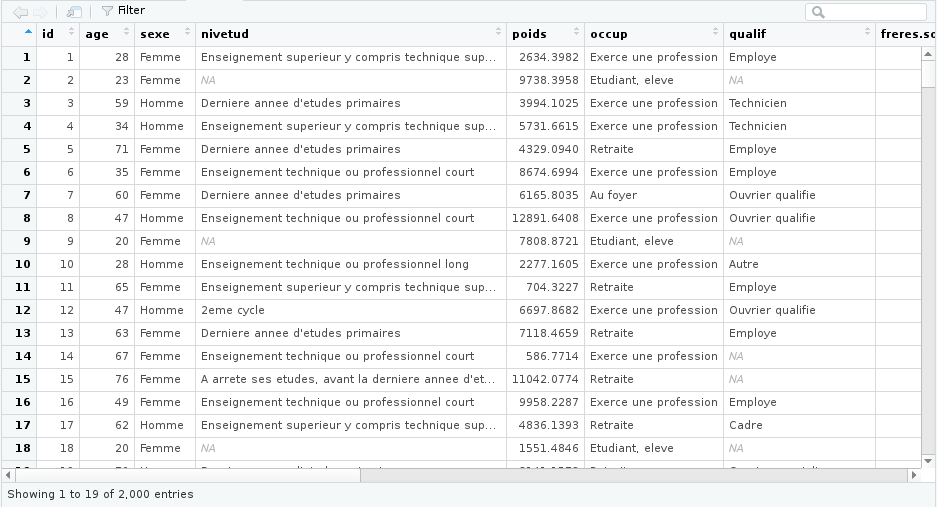
\includegraphics[keepaspectratio]{bases/ressources/rstudio_view_hdv2003.png}}

}

\caption{\label{fig-view}Interface View() de R RStudio}

\end{figure}%

Les fonctions \texttt{head()} et \texttt{tail()}, qui marchent également
sur les vecteurs, permettent d'afficher seulement les premières
(respectivement les dernières) lignes d'un tableau de données~:

\begin{Shaded}
\begin{Highlighting}[]
\FunctionTok{head}\NormalTok{(hdv2003)}
\end{Highlighting}
\end{Shaded}

\begin{verbatim}
  id age  sexe                                              nivetud    poids
1  1  28 Femme Enseignement superieur y compris technique superieur 2634.398
2  2  23 Femme                                                 <NA> 9738.396
3  3  59 Homme                    Derniere annee d'etudes primaires 3994.102
4  4  34 Homme Enseignement superieur y compris technique superieur 5731.662
5  5  71 Femme                    Derniere annee d'etudes primaires 4329.094
6  6  35 Femme        Enseignement technique ou professionnel court 8674.699
                  occup     qualif freres.soeurs clso
1 Exerce une profession    Employe             8  Oui
2       Etudiant, eleve       <NA>             2  Oui
3 Exerce une profession Technicien             2  Non
4 Exerce une profession Technicien             1  Non
5              Retraite    Employe             0  Oui
6 Exerce une profession    Employe             5  Non
                        relig                     trav.imp    trav.satisf
1 Ni croyance ni appartenance                Peu important Insatisfaction
2 Ni croyance ni appartenance                         <NA>           <NA>
3 Ni croyance ni appartenance Aussi important que le reste      Equilibre
4  Appartenance sans pratique Moins important que le reste   Satisfaction
5         Pratiquant regulier                         <NA>           <NA>
6 Ni croyance ni appartenance            Le plus important      Equilibre
  hard.rock lecture.bd peche.chasse cuisine bricol cinema sport heures.tv
1       Non        Non          Non     Oui    Non    Non   Non         0
2       Non        Non          Non     Non    Non    Oui   Oui         1
3       Non        Non          Non     Non    Non    Non   Oui         0
4       Non        Non          Non     Oui    Oui    Oui   Oui         2
5       Non        Non          Non     Non    Non    Non   Non         3
6       Non        Non          Non     Non    Non    Oui   Oui         2
\end{verbatim}

\begin{Shaded}
\begin{Highlighting}[]
\FunctionTok{tail}\NormalTok{(hdv2003, }\DecValTok{2}\NormalTok{)}
\end{Highlighting}
\end{Shaded}

\begin{verbatim}
       id age  sexe                                       nivetud     poids
1999 1999  24 Femme Enseignement technique ou professionnel court 13740.810
2000 2000  66 Femme  Enseignement technique ou professionnel long  7709.513
                     occup  qualif freres.soeurs clso
1999 Exerce une profession Employe             2  Non
2000              Au foyer Employe             3  Non
                          relig                     trav.imp trav.satisf
1999 Appartenance sans pratique Moins important que le reste   Equilibre
2000 Appartenance sans pratique                         <NA>        <NA>
     hard.rock lecture.bd peche.chasse cuisine bricol cinema sport heures.tv
1999       Non        Non          Non     Non    Non    Oui   Non       0.3
2000       Non        Oui          Non     Oui    Non    Non   Non       0.0
\end{verbatim}

L'extension \texttt{\{dplyr\}} propose une fonction
\texttt{dplyr::glimpse()} (ce qui signifie aperçu en anglais) qui permet
de visualiser rapidement et de manière condensée le contenu d'un tableau
de données.

\begin{Shaded}
\begin{Highlighting}[]
\FunctionTok{library}\NormalTok{(dplyr)}
\FunctionTok{glimpse}\NormalTok{(hdv2003)}
\end{Highlighting}
\end{Shaded}

\begin{verbatim}
Rows: 2,000
Columns: 20
$ id            <int> 1, 2, 3, 4, 5, 6, 7, 8, 9, 10, 11, 12, 13, 14, 15, 16, 1~
$ age           <int> 28, 23, 59, 34, 71, 35, 60, 47, 20, 28, 65, 47, 63, 67, ~
$ sexe          <fct> Femme, Femme, Homme, Homme, Femme, Femme, Femme, Homme, ~
$ nivetud       <fct> "Enseignement superieur y compris technique superieur", ~
$ poids         <dbl> 2634.3982, 9738.3958, 3994.1025, 5731.6615, 4329.0940, 8~
$ occup         <fct> "Exerce une profession", "Etudiant, eleve", "Exerce une ~
$ qualif        <fct> Employe, NA, Technicien, Technicien, Employe, Employe, O~
$ freres.soeurs <int> 8, 2, 2, 1, 0, 5, 1, 5, 4, 2, 3, 4, 1, 5, 2, 3, 4, 0, 2,~
$ clso          <fct> Oui, Oui, Non, Non, Oui, Non, Oui, Non, Oui, Non, Oui, O~
$ relig         <fct> Ni croyance ni appartenance, Ni croyance ni appartenance~
$ trav.imp      <fct> Peu important, NA, Aussi important que le reste, Moins i~
$ trav.satisf   <fct> Insatisfaction, NA, Equilibre, Satisfaction, NA, Equilib~
$ hard.rock     <fct> Non, Non, Non, Non, Non, Non, Non, Non, Non, Non, Non, N~
$ lecture.bd    <fct> Non, Non, Non, Non, Non, Non, Non, Non, Non, Non, Non, N~
$ peche.chasse  <fct> Non, Non, Non, Non, Non, Non, Oui, Oui, Non, Non, Non, N~
$ cuisine       <fct> Oui, Non, Non, Oui, Non, Non, Oui, Oui, Non, Non, Oui, N~
$ bricol        <fct> Non, Non, Non, Oui, Non, Non, Non, Oui, Non, Non, Oui, O~
$ cinema        <fct> Non, Oui, Non, Oui, Non, Oui, Non, Non, Oui, Oui, Oui, N~
$ sport         <fct> Non, Oui, Oui, Oui, Non, Oui, Non, Non, Non, Oui, Non, O~
$ heures.tv     <dbl> 0.0, 1.0, 0.0, 2.0, 3.0, 2.0, 2.9, 1.0, 2.0, 2.0, 1.0, 0~
\end{verbatim}

L'extension \texttt{\{labelled\}} propose une fonction
\texttt{labelled::look\_for()} qui permet de lister les différentes
variables d'un fichier de données~:

\begin{Shaded}
\begin{Highlighting}[]
\FunctionTok{library}\NormalTok{(labelled)}
\FunctionTok{look\_for}\NormalTok{(hdv2003)}
\end{Highlighting}
\end{Shaded}

\begin{verbatim}
 pos variable      label col_type missing values                              
 1   id            —     int      0                                           
 2   age           —     int      0                                           
 3   sexe          —     fct      0       Homme                               
                                          Femme                               
 4   nivetud       —     fct      112     N'a jamais fait d'etudes            
                                          A arrete ses etudes, avant la derni~
                                          Derniere annee d'etudes primaires   
                                          1er cycle                           
                                          2eme cycle                          
                                          Enseignement technique ou professio~
                                          Enseignement technique ou professio~
                                          Enseignement superieur y compris te~
 5   poids         —     dbl      0                                           
 6   occup         —     fct      0       Exerce une profession               
                                          Chomeur                             
                                          Etudiant, eleve                     
                                          Retraite                            
                                          Retire des affaires                 
                                          Au foyer                            
                                          Autre inactif                       
 7   qualif        —     fct      347     Ouvrier specialise                  
                                          Ouvrier qualifie                    
                                          Technicien                          
                                          Profession intermediaire            
                                          Cadre                               
                                          Employe                             
                                          Autre                               
 8   freres.soeurs —     int      0                                           
 9   clso          —     fct      0       Oui                                 
                                          Non                                 
                                          Ne sait pas                         
 10  relig         —     fct      0       Pratiquant regulier                 
                                          Pratiquant occasionnel              
                                          Appartenance sans pratique          
                                          Ni croyance ni appartenance         
                                          Rejet                               
                                          NSP ou NVPR                         
 11  trav.imp      —     fct      952     Le plus important                   
                                          Aussi important que le reste        
                                          Moins important que le reste        
                                          Peu important                       
 12  trav.satisf   —     fct      952     Satisfaction                        
                                          Insatisfaction                      
                                          Equilibre                           
 13  hard.rock     —     fct      0       Non                                 
                                          Oui                                 
 14  lecture.bd    —     fct      0       Non                                 
                                          Oui                                 
 15  peche.chasse  —     fct      0       Non                                 
                                          Oui                                 
 16  cuisine       —     fct      0       Non                                 
                                          Oui                                 
 17  bricol        —     fct      0       Non                                 
                                          Oui                                 
 18  cinema        —     fct      0       Non                                 
                                          Oui                                 
 19  sport         —     fct      0       Non                                 
                                          Oui                                 
 20  heures.tv     —     dbl      5                                           
\end{verbatim}

Lorsqu'on a un gros tableau de données avec de nombreuses variables, il
peut être difficile de retrouver la ou les variables d'intérêt. Il est
possible d'indiquer à \texttt{labelled::look\_for()} un mot-clé pour
limiter la recherche. Par exemple~:

\begin{Shaded}
\begin{Highlighting}[]
\FunctionTok{look\_for}\NormalTok{(hdv2003, }\StringTok{"trav"}\NormalTok{)}
\end{Highlighting}
\end{Shaded}

\begin{verbatim}
 pos variable    label col_type missing values                      
 11  trav.imp    —     fct      952     Le plus important           
                                        Aussi important que le reste
                                        Moins important que le reste
                                        Peu important               
 12  trav.satisf —     fct      952     Satisfaction                
                                        Insatisfaction              
                                        Equilibre                   
\end{verbatim}

Il est à noter que si la recherche n'est pas sensible à la casse
(i.e.~aux majuscules et aux minuscules), elle est sensible aux accents.

La méthode \texttt{summary()} qui fonctionne sur tout type d'objet
permet d'avoir quelques statistiques de base sur les différentes
variables de notre tableau, les statistiques affichées dépendant du type
de variable.

\begin{Shaded}
\begin{Highlighting}[]
\FunctionTok{summary}\NormalTok{(hdv2003)}
\end{Highlighting}
\end{Shaded}

\begin{verbatim}
       id              age           sexe     
 Min.   :   1.0   Min.   :18.00   Homme: 899  
 1st Qu.: 500.8   1st Qu.:35.00   Femme:1101  
 Median :1000.5   Median :48.00               
 Mean   :1000.5   Mean   :48.16               
 3rd Qu.:1500.2   3rd Qu.:60.00               
 Max.   :2000.0   Max.   :97.00               
                                              
                                                 nivetud        poids         
 Enseignement technique ou professionnel court       :463   Min.   :   78.08  
 Enseignement superieur y compris technique superieur:441   1st Qu.: 2221.82  
 Derniere annee d'etudes primaires                   :341   Median : 4631.19  
 1er cycle                                           :204   Mean   : 5535.61  
 2eme cycle                                          :183   3rd Qu.: 7626.53  
 (Other)                                             :256   Max.   :31092.14  
 NA's                                                :112                     
                   occup                           qualif    freres.soeurs   
 Exerce une profession:1049   Employe                 :594   Min.   : 0.000  
 Chomeur              : 134   Ouvrier qualifie        :292   1st Qu.: 1.000  
 Etudiant, eleve      :  94   Cadre                   :260   Median : 2.000  
 Retraite             : 392   Ouvrier specialise      :203   Mean   : 3.283  
 Retire des affaires  :  77   Profession intermediaire:160   3rd Qu.: 5.000  
 Au foyer             : 171   (Other)                 :144   Max.   :22.000  
 Autre inactif        :  83   NA's                    :347                   
          clso                              relig    
 Oui        : 936   Pratiquant regulier        :266  
 Non        :1037   Pratiquant occasionnel     :442  
 Ne sait pas:  27   Appartenance sans pratique :760  
                    Ni croyance ni appartenance:399  
                    Rejet                      : 93  
                    NSP ou NVPR                : 40  
                                                     
                         trav.imp           trav.satisf  hard.rock  lecture.bd
 Le plus important           : 29   Satisfaction  :480   Non:1986   Non:1953  
 Aussi important que le reste:259   Insatisfaction:117   Oui:  14   Oui:  47  
 Moins important que le reste:708   Equilibre     :451                        
 Peu important               : 52   NA's          :952                        
 NA's                        :952                                             
                                                                              
                                                                              
 peche.chasse cuisine    bricol     cinema     sport        heures.tv     
 Non:1776     Non:1119   Non:1147   Non:1174   Non:1277   Min.   : 0.000  
 Oui: 224     Oui: 881   Oui: 853   Oui: 826   Oui: 723   1st Qu.: 1.000  
                                                          Median : 2.000  
                                                          Mean   : 2.247  
                                                          3rd Qu.: 3.000  
                                                          Max.   :12.000  
                                                          NA's   :5       
\end{verbatim}

On peut également appliquer \texttt{summary()} à une variable
particulière.

\begin{Shaded}
\begin{Highlighting}[]
\FunctionTok{summary}\NormalTok{(hdv2003}\SpecialCharTok{$}\NormalTok{sexe)}
\end{Highlighting}
\end{Shaded}

\begin{verbatim}
Homme Femme 
  899  1101 
\end{verbatim}

\begin{Shaded}
\begin{Highlighting}[]
\FunctionTok{summary}\NormalTok{(hdv2003}\SpecialCharTok{$}\NormalTok{age)}
\end{Highlighting}
\end{Shaded}

\begin{verbatim}
   Min. 1st Qu.  Median    Mean 3rd Qu.    Max. 
  18.00   35.00   48.00   48.16   60.00   97.00 
\end{verbatim}

\section{En résumé}\label{en-ruxe9sumuxe9-2}

\begin{itemize}
\tightlist
\item
  Les tableaux de données sont des listes avec des propriétés
  particulières~:

  \begin{enumerate}
  \def\labelenumi{\roman{enumi}.}
  \tightlist
  \item
    tous les éléments sont des vecteurs~;
  \item
    tous les vecteurs ont la même longueur~;
  \item
    tous les vecteurs ont un nom et ce nom est unique.
  \end{enumerate}
\item
  On peut créer un tableau de données avec \texttt{data.frame()}.
\item
  Les tableaux de données correspondent aux fichiers de données qu'on
  utilise usuellement dans d'autres logiciels de statistiques~: les
  variables sont représentées en colonnes et les observations en lignes.
\item
  Ce sont des objets bidimensionnels~: \texttt{ncol()} renvoie le nombre
  de colonnes et \texttt{nrow()} le nombre de lignes.
\item
  Les doubles crochets (\texttt{{[}{[}{]}{]}}) et le symbole dollar
  (\texttt{\$}) fonctionnent comme pour les listes et permettent
  d'accéder aux variables.
\item
  Il est possible d'utiliser des coordonnées bidimensionnelles avec les
  crochets simples (\texttt{{[}{]}}) en indiquant un critère sur les
  lignes puis un critère sur les colonnes, séparés par une virgule
  (\texttt{,}).
\end{itemize}

\section{webin-R}\label{webin-r-2}

On pourra également se référer au webin-R \#02 (\emph{les bases du
langage R}) sur \href{https://youtu.be/Eh8piunoqQc}{YouTube}.

\url{https://youtu.be/Eh8piunoqQc}

\chapter{Tibbles}\label{sec-tibbles}

\section{Le concept de tidy data}\label{sec-tidy-data}

Le \texttt{\{tidyverse\}} est en partie fondé sur le concept de
\emph{tidy data}, développé à l'origine par Hadley Wickham dans un
\href{https://www.jstatsoft.org/article/view/v059i10}{article de 2014}
du \emph{Journal of Statistical Software}.

Il s'agit d'un modèle d'organisation des données qui vise à faciliter le
travail souvent long et fastidieux de nettoyage et de préparation
préalable à la mise en oeuvre de méthodes d'analyse.

Les principes d'un jeu de données \emph{tidy} sont les suivants~:

\begin{enumerate}
\def\labelenumi{\arabic{enumi}.}
\tightlist
\item
  chaque variable est une colonne
\item
  chaque observation est une ligne
\item
  chaque type d'observation est dans une table différente
\end{enumerate}

Un chapitre dédié à \texttt{\{tidyr\}} (voir Chapitre~\ref{sec-tidyr})
présente comment définir et rendre des données \emph{tidy} avec ce
package.

Les extensions du \texttt{\{tidyverse\}}, notamment \texttt{\{ggplot2\}}
et \texttt{\{dplyr\}}, sont prévues pour fonctionner avec des données
\emph{tidy}.

\section{tibbles~: des tableaux de données améliorés}\label{tibbles}

Une autre particularité du \texttt{\{tidyverse\}} est que ces extensions
travaillent avec des tableaux de données au format
\texttt{tibble::tibble()}, qui est une évolution plus moderne du
classique \texttt{data.frame} de \textbf{R} de base.

Ce format est fourni est géré par l'extension du même nom
(\texttt{\{tibble\}}), qui fait partie du cœur du \emph{tidyverse}. La
plupart des fonctions des extensions du \emph{tidyverse} acceptent des
\emph{data.frames} en entrée, mais retournent un \emph{tibble}.

Contrairement aux \emph{data frames}, les \emph{tibbles}~:

\begin{itemize}
\tightlist
\item
  n'ont pas de noms de lignes (\emph{rownames})
\item
  autorisent des noms de colonnes invalides pour les \emph{data frames}
  (espaces, caractères spéciaux, nombres\ldots) \footnote{Quand on veut
    utiliser des noms de ce type, on doit les entourer avec des
    \emph{backticks} (`)}
\item
  s'affichent plus intelligemment que les \emph{data frames}~: seules
  les premières lignes sont affichées, ainsi que quelques informations
  supplémentaires utiles (dimensions, types des colonnes\ldots)
\item
  ne font pas de \emph{partial matching} sur les noms de colonnes
  \footnote{Dans \textbf{R} base, si une table \texttt{d} contient une
    colonne \texttt{qualif}, \texttt{d\$qual} retournera cette colonne.}
\item
  affichent un avertissement si on essaie d'accéder à une colonne qui
  n'existe pas
\end{itemize}

Pour autant, les tibbles restent compatibles avec les \emph{data
frames}.

Il est possible de créer un \emph{tibble} manuellement avec
\texttt{tibble::tibble()}.

\begin{Shaded}
\begin{Highlighting}[]
\FunctionTok{library}\NormalTok{(tidyverse)}
\FunctionTok{tibble}\NormalTok{(}
  \AttributeTok{x =} \FunctionTok{c}\NormalTok{(}\FloatTok{1.2345}\NormalTok{, }\FloatTok{12.345}\NormalTok{, }\FloatTok{123.45}\NormalTok{, }\FloatTok{1234.5}\NormalTok{, }\DecValTok{12345}\NormalTok{),}
  \AttributeTok{y =} \FunctionTok{c}\NormalTok{(}\StringTok{"a"}\NormalTok{, }\StringTok{"b"}\NormalTok{, }\StringTok{"c"}\NormalTok{, }\StringTok{"d"}\NormalTok{, }\StringTok{"e"}\NormalTok{)}
\NormalTok{)}
\end{Highlighting}
\end{Shaded}

\begin{verbatim}
# A tibble: 5 x 2
         x y    
     <dbl> <chr>
1     1.23 a    
2    12.3  b    
3   123.   c    
4  1234.   d    
5 12345    e    
\end{verbatim}

On peut ainsi facilement convertir un \emph{data frame} en tibble avec
\texttt{tibble::as\_tibble()}~:

\begin{Shaded}
\begin{Highlighting}[]
\NormalTok{d }\OtherTok{\textless{}{-}} \FunctionTok{as\_tibble}\NormalTok{(mtcars)}
\NormalTok{d}
\end{Highlighting}
\end{Shaded}

\begin{verbatim}
# A tibble: 32 x 11
     mpg   cyl  disp    hp  drat    wt  qsec    vs    am  gear  carb
   <dbl> <dbl> <dbl> <dbl> <dbl> <dbl> <dbl> <dbl> <dbl> <dbl> <dbl>
 1  21       6  160    110  3.9   2.62  16.5     0     1     4     4
 2  21       6  160    110  3.9   2.88  17.0     0     1     4     4
 3  22.8     4  108     93  3.85  2.32  18.6     1     1     4     1
 4  21.4     6  258    110  3.08  3.22  19.4     1     0     3     1
 5  18.7     8  360    175  3.15  3.44  17.0     0     0     3     2
 6  18.1     6  225    105  2.76  3.46  20.2     1     0     3     1
 7  14.3     8  360    245  3.21  3.57  15.8     0     0     3     4
 8  24.4     4  147.    62  3.69  3.19  20       1     0     4     2
 9  22.8     4  141.    95  3.92  3.15  22.9     1     0     4     2
10  19.2     6  168.   123  3.92  3.44  18.3     1     0     4     4
# i 22 more rows
\end{verbatim}

D'ailleurs, quand on regarde la classe d'un tibble, on peut s'apercevoir
qu'un tibble hérite de la classe \texttt{data.frame} mais possède en
plus la classe \texttt{tbl\_df}. Cela traduit bien le fait que les
\emph{tibbles} restent des \emph{data frames}.

\begin{Shaded}
\begin{Highlighting}[]
\FunctionTok{class}\NormalTok{(d)}
\end{Highlighting}
\end{Shaded}

\begin{verbatim}
[1] "tbl_df"     "tbl"        "data.frame"
\end{verbatim}

Si le \emph{data frame} d'origine a des \emph{rownames}, on peut d'abord
les convertir en colonnes avec \texttt{tibble::rownames\_to\_column()}~:

\begin{Shaded}
\begin{Highlighting}[]
\NormalTok{d }\OtherTok{\textless{}{-}} \FunctionTok{as\_tibble}\NormalTok{(}\FunctionTok{rownames\_to\_column}\NormalTok{(mtcars))}
\NormalTok{d}
\end{Highlighting}
\end{Shaded}

\begin{verbatim}
# A tibble: 32 x 12
   rowname       mpg   cyl  disp    hp  drat    wt  qsec    vs    am  gear  carb
   <chr>       <dbl> <dbl> <dbl> <dbl> <dbl> <dbl> <dbl> <dbl> <dbl> <dbl> <dbl>
 1 Mazda RX4    21       6  160    110  3.9   2.62  16.5     0     1     4     4
 2 Mazda RX4 ~  21       6  160    110  3.9   2.88  17.0     0     1     4     4
 3 Datsun 710   22.8     4  108     93  3.85  2.32  18.6     1     1     4     1
 4 Hornet 4 D~  21.4     6  258    110  3.08  3.22  19.4     1     0     3     1
 5 Hornet Spo~  18.7     8  360    175  3.15  3.44  17.0     0     0     3     2
 6 Valiant      18.1     6  225    105  2.76  3.46  20.2     1     0     3     1
 7 Duster 360   14.3     8  360    245  3.21  3.57  15.8     0     0     3     4
 8 Merc 240D    24.4     4  147.    62  3.69  3.19  20       1     0     4     2
 9 Merc 230     22.8     4  141.    95  3.92  3.15  22.9     1     0     4     2
10 Merc 280     19.2     6  168.   123  3.92  3.44  18.3     1     0     4     4
# i 22 more rows
\end{verbatim}

À l'inverse, on peut à tout moment convertir un tibble en \emph{data
frame} avec \texttt{tibble::as.data.frame()}~:

\begin{Shaded}
\begin{Highlighting}[]
\FunctionTok{as.data.frame}\NormalTok{(d)}
\end{Highlighting}
\end{Shaded}

\begin{verbatim}
               rowname  mpg cyl  disp  hp drat    wt  qsec vs am gear carb
1            Mazda RX4 21.0   6 160.0 110 3.90 2.620 16.46  0  1    4    4
2        Mazda RX4 Wag 21.0   6 160.0 110 3.90 2.875 17.02  0  1    4    4
3           Datsun 710 22.8   4 108.0  93 3.85 2.320 18.61  1  1    4    1
4       Hornet 4 Drive 21.4   6 258.0 110 3.08 3.215 19.44  1  0    3    1
5    Hornet Sportabout 18.7   8 360.0 175 3.15 3.440 17.02  0  0    3    2
6              Valiant 18.1   6 225.0 105 2.76 3.460 20.22  1  0    3    1
7           Duster 360 14.3   8 360.0 245 3.21 3.570 15.84  0  0    3    4
8            Merc 240D 24.4   4 146.7  62 3.69 3.190 20.00  1  0    4    2
9             Merc 230 22.8   4 140.8  95 3.92 3.150 22.90  1  0    4    2
10            Merc 280 19.2   6 167.6 123 3.92 3.440 18.30  1  0    4    4
11           Merc 280C 17.8   6 167.6 123 3.92 3.440 18.90  1  0    4    4
12          Merc 450SE 16.4   8 275.8 180 3.07 4.070 17.40  0  0    3    3
13          Merc 450SL 17.3   8 275.8 180 3.07 3.730 17.60  0  0    3    3
14         Merc 450SLC 15.2   8 275.8 180 3.07 3.780 18.00  0  0    3    3
15  Cadillac Fleetwood 10.4   8 472.0 205 2.93 5.250 17.98  0  0    3    4
16 Lincoln Continental 10.4   8 460.0 215 3.00 5.424 17.82  0  0    3    4
17   Chrysler Imperial 14.7   8 440.0 230 3.23 5.345 17.42  0  0    3    4
18            Fiat 128 32.4   4  78.7  66 4.08 2.200 19.47  1  1    4    1
19         Honda Civic 30.4   4  75.7  52 4.93 1.615 18.52  1  1    4    2
20      Toyota Corolla 33.9   4  71.1  65 4.22 1.835 19.90  1  1    4    1
21       Toyota Corona 21.5   4 120.1  97 3.70 2.465 20.01  1  0    3    1
22    Dodge Challenger 15.5   8 318.0 150 2.76 3.520 16.87  0  0    3    2
23         AMC Javelin 15.2   8 304.0 150 3.15 3.435 17.30  0  0    3    2
24          Camaro Z28 13.3   8 350.0 245 3.73 3.840 15.41  0  0    3    4
25    Pontiac Firebird 19.2   8 400.0 175 3.08 3.845 17.05  0  0    3    2
26           Fiat X1-9 27.3   4  79.0  66 4.08 1.935 18.90  1  1    4    1
27       Porsche 914-2 26.0   4 120.3  91 4.43 2.140 16.70  0  1    5    2
28        Lotus Europa 30.4   4  95.1 113 3.77 1.513 16.90  1  1    5    2
29      Ford Pantera L 15.8   8 351.0 264 4.22 3.170 14.50  0  1    5    4
30        Ferrari Dino 19.7   6 145.0 175 3.62 2.770 15.50  0  1    5    6
31       Maserati Bora 15.0   8 301.0 335 3.54 3.570 14.60  0  1    5    8
32          Volvo 142E 21.4   4 121.0 109 4.11 2.780 18.60  1  1    4    2
\end{verbatim}

Là encore, on peut convertir la colonne \emph{rowname} en ``vrais''
\emph{rownames} avec \texttt{tibble::column\_to\_rownames()}~:

\begin{Shaded}
\begin{Highlighting}[]
\FunctionTok{column\_to\_rownames}\NormalTok{(}\FunctionTok{as.data.frame}\NormalTok{(d))}
\end{Highlighting}
\end{Shaded}

\begin{verbatim}
                     mpg cyl  disp  hp drat    wt  qsec vs am gear carb
Mazda RX4           21.0   6 160.0 110 3.90 2.620 16.46  0  1    4    4
Mazda RX4 Wag       21.0   6 160.0 110 3.90 2.875 17.02  0  1    4    4
Datsun 710          22.8   4 108.0  93 3.85 2.320 18.61  1  1    4    1
Hornet 4 Drive      21.4   6 258.0 110 3.08 3.215 19.44  1  0    3    1
Hornet Sportabout   18.7   8 360.0 175 3.15 3.440 17.02  0  0    3    2
Valiant             18.1   6 225.0 105 2.76 3.460 20.22  1  0    3    1
Duster 360          14.3   8 360.0 245 3.21 3.570 15.84  0  0    3    4
Merc 240D           24.4   4 146.7  62 3.69 3.190 20.00  1  0    4    2
Merc 230            22.8   4 140.8  95 3.92 3.150 22.90  1  0    4    2
Merc 280            19.2   6 167.6 123 3.92 3.440 18.30  1  0    4    4
Merc 280C           17.8   6 167.6 123 3.92 3.440 18.90  1  0    4    4
Merc 450SE          16.4   8 275.8 180 3.07 4.070 17.40  0  0    3    3
Merc 450SL          17.3   8 275.8 180 3.07 3.730 17.60  0  0    3    3
Merc 450SLC         15.2   8 275.8 180 3.07 3.780 18.00  0  0    3    3
Cadillac Fleetwood  10.4   8 472.0 205 2.93 5.250 17.98  0  0    3    4
Lincoln Continental 10.4   8 460.0 215 3.00 5.424 17.82  0  0    3    4
Chrysler Imperial   14.7   8 440.0 230 3.23 5.345 17.42  0  0    3    4
Fiat 128            32.4   4  78.7  66 4.08 2.200 19.47  1  1    4    1
Honda Civic         30.4   4  75.7  52 4.93 1.615 18.52  1  1    4    2
Toyota Corolla      33.9   4  71.1  65 4.22 1.835 19.90  1  1    4    1
Toyota Corona       21.5   4 120.1  97 3.70 2.465 20.01  1  0    3    1
Dodge Challenger    15.5   8 318.0 150 2.76 3.520 16.87  0  0    3    2
AMC Javelin         15.2   8 304.0 150 3.15 3.435 17.30  0  0    3    2
Camaro Z28          13.3   8 350.0 245 3.73 3.840 15.41  0  0    3    4
Pontiac Firebird    19.2   8 400.0 175 3.08 3.845 17.05  0  0    3    2
Fiat X1-9           27.3   4  79.0  66 4.08 1.935 18.90  1  1    4    1
Porsche 914-2       26.0   4 120.3  91 4.43 2.140 16.70  0  1    5    2
Lotus Europa        30.4   4  95.1 113 3.77 1.513 16.90  1  1    5    2
Ford Pantera L      15.8   8 351.0 264 4.22 3.170 14.50  0  1    5    4
Ferrari Dino        19.7   6 145.0 175 3.62 2.770 15.50  0  1    5    6
Maserati Bora       15.0   8 301.0 335 3.54 3.570 14.60  0  1    5    8
Volvo 142E          21.4   4 121.0 109 4.11 2.780 18.60  1  1    4    2
\end{verbatim}

\begin{tcolorbox}[enhanced jigsaw, toptitle=1mm, bottomtitle=1mm, colframe=quarto-callout-note-color-frame, toprule=.15mm, left=2mm, bottomrule=.15mm, opacitybacktitle=0.6, opacityback=0, coltitle=black, breakable, rightrule=.15mm, arc=.35mm, title=\textcolor{quarto-callout-note-color}{\faInfo}\hspace{0.5em}{Note}, colbacktitle=quarto-callout-note-color!10!white, titlerule=0mm, leftrule=.75mm, colback=white]

Les deux fonctions \texttt{tibble::column\_to\_rownames()} et
\texttt{tibble::rownames\_to\_column()} acceptent un argument
supplémentaire \texttt{var} qui permet d'indiquer un nom de colonne
autre que le nom \texttt{rowname} utilisé par défaut pour créer ou
identifier la colonne contenant les noms de lignes.

\end{tcolorbox}

\section{Données et tableaux
imbriqués}\label{donnuxe9es-et-tableaux-imbriquuxe9s}

Une des particularités des \emph{tibbles} est qu'ils acceptent, à la
différence des \emph{data frames}, des colonnes composées de listes et,
par extension, d'autres tibbles (qui sont des listes) ~!

\begin{Shaded}
\begin{Highlighting}[]
\NormalTok{d }\OtherTok{\textless{}{-}} \FunctionTok{tibble}\NormalTok{(}
  \AttributeTok{g =} \FunctionTok{c}\NormalTok{(}\DecValTok{1}\NormalTok{, }\DecValTok{2}\NormalTok{, }\DecValTok{3}\NormalTok{),}
  \AttributeTok{data =} \FunctionTok{list}\NormalTok{(}
    \FunctionTok{tibble}\NormalTok{(}\AttributeTok{x =} \DecValTok{1}\NormalTok{, }\AttributeTok{y =} \DecValTok{2}\NormalTok{),}
    \FunctionTok{tibble}\NormalTok{(}\AttributeTok{x =} \DecValTok{4}\SpecialCharTok{:}\DecValTok{5}\NormalTok{, }\AttributeTok{y =} \DecValTok{6}\SpecialCharTok{:}\DecValTok{7}\NormalTok{),}
    \FunctionTok{tibble}\NormalTok{(}\AttributeTok{x =} \DecValTok{10}\NormalTok{)}
\NormalTok{  )}
\NormalTok{)}
\NormalTok{d}
\end{Highlighting}
\end{Shaded}

\begin{verbatim}
# A tibble: 3 x 2
      g data            
  <dbl> <list>          
1     1 <tibble [1 x 2]>
2     2 <tibble [2 x 2]>
3     3 <tibble [1 x 1]>
\end{verbatim}

\begin{Shaded}
\begin{Highlighting}[]
\NormalTok{d}\SpecialCharTok{$}\NormalTok{data[[}\DecValTok{2}\NormalTok{]]}
\end{Highlighting}
\end{Shaded}

\begin{verbatim}
# A tibble: 2 x 2
      x     y
  <int> <int>
1     4     6
2     5     7
\end{verbatim}

Cette fonctionnalité, combinée avec les fonctions de \texttt{\{tidyr\}}
et de \texttt{\{purrr\}}, s'avère très puissante pour réaliser des
opérations multiples en peu de ligne de code.

Dans l'exemple ci-dessous, nous réalisons des régressions linéaires par
sous-groupe et les présentons dans un même tableau. Pour le moment, le
code présenté doit vous sembler complexe et un peu obscur. Pas de
panique : tout cela sera clarifié dans les différents chapitres de ce
guide. Ce qu'il y a à retenir pour le moment, c'est la possibilité de
stocker, dans les colonnes d'un \emph{tibble}, différent types de
données, y compris des sous-tableaux, des résultats de modèles et même
des tableaux mis en forme.

\begin{Shaded}
\begin{Highlighting}[]
\NormalTok{reg }\OtherTok{\textless{}{-}}
\NormalTok{  iris }\SpecialCharTok{|\textgreater{}} 
  \FunctionTok{group\_by}\NormalTok{(Species) }\SpecialCharTok{|\textgreater{}} 
  \FunctionTok{nest}\NormalTok{() }\SpecialCharTok{|\textgreater{}} 
  \FunctionTok{mutate}\NormalTok{(}
    \AttributeTok{model =} \FunctionTok{map}\NormalTok{(}
\NormalTok{      data, }
      \SpecialCharTok{\textasciitilde{}} \FunctionTok{lm}\NormalTok{(Sepal.Length }\SpecialCharTok{\textasciitilde{}}\NormalTok{ Petal.Length }\SpecialCharTok{+}\NormalTok{ Petal.Width, }\AttributeTok{data =}\NormalTok{ .)}
\NormalTok{    ),}
    \AttributeTok{tbl =} \FunctionTok{map}\NormalTok{(model, gtsummary}\SpecialCharTok{::}\NormalTok{tbl\_regression)}
\NormalTok{  )}
\NormalTok{reg}
\end{Highlighting}
\end{Shaded}

\begin{verbatim}
# A tibble: 3 x 4
# Groups:   Species [3]
  Species    data              model  tbl       
  <fct>      <list>            <list> <list>    
1 setosa     <tibble [50 x 4]> <lm>   <tbl_rgrs>
2 versicolor <tibble [50 x 4]> <lm>   <tbl_rgrs>
3 virginica  <tibble [50 x 4]> <lm>   <tbl_rgrs>
\end{verbatim}

\begin{Shaded}
\begin{Highlighting}[]
\NormalTok{gtsummary}\SpecialCharTok{::}\FunctionTok{tbl\_merge}\NormalTok{(}
\NormalTok{  reg}\SpecialCharTok{$}\NormalTok{tbl,}
  \AttributeTok{tab\_spanner =} \FunctionTok{paste0}\NormalTok{(}\StringTok{"**"}\NormalTok{, reg}\SpecialCharTok{$}\NormalTok{Species, }\StringTok{"**"}\NormalTok{)}
\NormalTok{)}
\end{Highlighting}
\end{Shaded}

\begingroup
\fontsize{12.0pt}{14.4pt}\selectfont
\setlength{\LTpost}{0mm}
\begin{longtable*}{lccccccccc}
\toprule
 & \multicolumn{3}{c}{\textbf{setosa}} & \multicolumn{3}{c}{\textbf{versicolor}} & \multicolumn{3}{c}{\textbf{virginica}} \\ 
\cmidrule(lr){2-4} \cmidrule(lr){5-7} \cmidrule(lr){8-10}
\textbf{Characteristic} & \textbf{Beta} & \textbf{95\% CI}\textsuperscript{\textit{1}} & \textbf{p-value} & \textbf{Beta} & \textbf{95\% CI}\textsuperscript{\textit{1}} & \textbf{p-value} & \textbf{Beta} & \textbf{95\% CI}\textsuperscript{\textit{1}} & \textbf{p-value} \\ 
\midrule\addlinespace[2.5pt]
Petal.Length & 0.40 & -0.20, 0.99 & 0.2 & 0.93 & 0.59, 1.3 & <0.001 & 1.0 & 0.81, 1.2 & <0.001 \\ 
Petal.Width & 0.71 & -0.27, 1.7 & 0.2 & -0.32 & -1.1, 0.49 & 0.4 & 0.01 & -0.35, 0.37 & >0.9 \\ 
\bottomrule
\end{longtable*}
\begin{minipage}{\linewidth}
\textsuperscript{\textit{1}}CI = Confidence Interval\\
\end{minipage}
\endgroup

\chapter{Attributs}\label{sec-attributs}

Les objets \textbf{R} peuvent avoir des attributs qui correspondent en
quelque sorte à des métadonnées associées à l'objet en question.
Techniquement, un attribut peut être tout type d'objet \textbf{R} (un
vecteur, une liste, une fonction\ldots).

Parmi les attributs les plus courants, on retrouve notamment~:

\begin{itemize}
\tightlist
\item
  \texttt{class}~: la classe de l'objet
\item
  \texttt{length}~: sa longueur
\item
  \texttt{names}~: les noms donnés aux éléments de l'objet
\item
  \texttt{levels}~: pour les facteurs, les étiquettes des différents
  niveaux
\item
  \texttt{label}~: une étiquette de variable
\end{itemize}

La fonction \texttt{attributes()} permet de lister tous les attributs
associés à un objet.

\begin{Shaded}
\begin{Highlighting}[]
\FunctionTok{attributes}\NormalTok{(iris)}
\end{Highlighting}
\end{Shaded}

\begin{verbatim}
$names
[1] "Sepal.Length" "Sepal.Width"  "Petal.Length" "Petal.Width"  "Species"     

$class
[1] "data.frame"

$row.names
  [1]   1   2   3   4   5   6   7   8   9  10  11  12  13  14  15  16  17  18
 [19]  19  20  21  22  23  24  25  26  27  28  29  30  31  32  33  34  35  36
 [37]  37  38  39  40  41  42  43  44  45  46  47  48  49  50  51  52  53  54
 [55]  55  56  57  58  59  60  61  62  63  64  65  66  67  68  69  70  71  72
 [73]  73  74  75  76  77  78  79  80  81  82  83  84  85  86  87  88  89  90
 [91]  91  92  93  94  95  96  97  98  99 100 101 102 103 104 105 106 107 108
[109] 109 110 111 112 113 114 115 116 117 118 119 120 121 122 123 124 125 126
[127] 127 128 129 130 131 132 133 134 135 136 137 138 139 140 141 142 143 144
[145] 145 146 147 148 149 150
\end{verbatim}

Pour accéder à un attribut spécifique, on aura recours à \texttt{attr()}
en spécifiant à la fois l'objet considéré et le nom de l'attribut
souhaité.

\begin{Shaded}
\begin{Highlighting}[]
\NormalTok{iris }\SpecialCharTok{|\textgreater{}} \FunctionTok{attr}\NormalTok{(}\StringTok{"names"}\NormalTok{)}
\end{Highlighting}
\end{Shaded}

\begin{verbatim}
[1] "Sepal.Length" "Sepal.Width"  "Petal.Length" "Petal.Width"  "Species"     
\end{verbatim}

Pour les attributs les plus courants de \textbf{R}, il faut noter qu'il
existe le plus souvent des fonctions spécifiques, comme
\texttt{class()}, \texttt{names()} ou \texttt{row.names()}.

\begin{Shaded}
\begin{Highlighting}[]
\FunctionTok{class}\NormalTok{(iris)}
\end{Highlighting}
\end{Shaded}

\begin{verbatim}
[1] "data.frame"
\end{verbatim}

\begin{Shaded}
\begin{Highlighting}[]
\FunctionTok{names}\NormalTok{(iris)}
\end{Highlighting}
\end{Shaded}

\begin{verbatim}
[1] "Sepal.Length" "Sepal.Width"  "Petal.Length" "Petal.Width"  "Species"     
\end{verbatim}

La fonction \texttt{attr()}, associée à l'opérateur d'assignation
(\texttt{\textless{}-}) permet également de définir ses propres
attributs.

\begin{Shaded}
\begin{Highlighting}[]
\FunctionTok{attr}\NormalTok{(iris, }\StringTok{"perso"}\NormalTok{) }\OtherTok{\textless{}{-}} \StringTok{"Des notes personnelles"}
\FunctionTok{attributes}\NormalTok{(iris)}
\end{Highlighting}
\end{Shaded}

\begin{verbatim}
$names
[1] "Sepal.Length" "Sepal.Width"  "Petal.Length" "Petal.Width"  "Species"     

$class
[1] "data.frame"

$row.names
  [1]   1   2   3   4   5   6   7   8   9  10  11  12  13  14  15  16  17  18
 [19]  19  20  21  22  23  24  25  26  27  28  29  30  31  32  33  34  35  36
 [37]  37  38  39  40  41  42  43  44  45  46  47  48  49  50  51  52  53  54
 [55]  55  56  57  58  59  60  61  62  63  64  65  66  67  68  69  70  71  72
 [73]  73  74  75  76  77  78  79  80  81  82  83  84  85  86  87  88  89  90
 [91]  91  92  93  94  95  96  97  98  99 100 101 102 103 104 105 106 107 108
[109] 109 110 111 112 113 114 115 116 117 118 119 120 121 122 123 124 125 126
[127] 127 128 129 130 131 132 133 134 135 136 137 138 139 140 141 142 143 144
[145] 145 146 147 148 149 150

$perso
[1] "Des notes personnelles"
\end{verbatim}

\begin{Shaded}
\begin{Highlighting}[]
\FunctionTok{attr}\NormalTok{(iris, }\StringTok{"perso"}\NormalTok{)}
\end{Highlighting}
\end{Shaded}

\begin{verbatim}
[1] "Des notes personnelles"
\end{verbatim}

\part{\textbf{Manipulation de données}}

\chapter{Le pipe}\label{sec-pipe}

Il est fréquent d'enchaîner des opérations en appelant successivement
des fonctions sur le résultat de l'appel précédent.

Prenons un exemple. Supposons que nous ayons un vecteur numérique
\texttt{v} dont nous voulons calculer la moyenne puis l'afficher via un
message dans la console. Pour un meilleur rendu, nous allons arrondir la
moyenne à une décimale, mettre en forme le résultat à la française,
c'est-à-dire avec la virgule comme séparateur des décimales, créer une
phrase avec le résultat, puis l'afficher dans la console. Voici le code
correspondant, étape par étape.

\begin{Shaded}
\begin{Highlighting}[]
\NormalTok{v }\OtherTok{\textless{}{-}} \FunctionTok{c}\NormalTok{(}\FloatTok{1.2}\NormalTok{, }\FloatTok{8.7}\NormalTok{, }\FloatTok{5.6}\NormalTok{, }\FloatTok{11.4}\NormalTok{)}
\NormalTok{m }\OtherTok{\textless{}{-}} \FunctionTok{mean}\NormalTok{(v)}
\NormalTok{r }\OtherTok{\textless{}{-}} \FunctionTok{round}\NormalTok{(m, }\AttributeTok{digits =} \DecValTok{1}\NormalTok{)}
\NormalTok{f }\OtherTok{\textless{}{-}} \FunctionTok{format}\NormalTok{(r, }\AttributeTok{decimal.mark =} \StringTok{","}\NormalTok{)}
\NormalTok{p }\OtherTok{\textless{}{-}} \FunctionTok{paste0}\NormalTok{(}\StringTok{"La moyenne est de "}\NormalTok{, f, }\StringTok{"."}\NormalTok{)}
\FunctionTok{message}\NormalTok{(p)}
\end{Highlighting}
\end{Shaded}

\begin{verbatim}
La moyenne est de 6,7.
\end{verbatim}

Cette écriture, n'est pas vraiment optimale, car cela entraîne la
création d'un grand nombre de variables intermédiaires totalement
inutiles. Nous pourrions dès lors imbriquer les différentes fonctions
les unes dans les autres~:

\begin{Shaded}
\begin{Highlighting}[]
\FunctionTok{message}\NormalTok{(}\FunctionTok{paste0}\NormalTok{(}\StringTok{"La moyenne est de "}\NormalTok{, }\FunctionTok{format}\NormalTok{(}\FunctionTok{round}\NormalTok{(}\FunctionTok{mean}\NormalTok{(v),        }\AttributeTok{digits =} \DecValTok{1}\NormalTok{), }\AttributeTok{decimal.mark =} \StringTok{","}\NormalTok{), }\StringTok{"."}\NormalTok{))}
\end{Highlighting}
\end{Shaded}

\begin{verbatim}
La moyenne est de 6,7.
\end{verbatim}

Nous obtenons bien le même résultat, mais la lecture de cette ligne de
code est assez difficile et il n'est pas aisé de bien identifier à
quelle fonction est rattaché chaque argument.

Une amélioration possible serait d'effectuer des retours à la ligne avec
une indentation adéquate pour rendre cela plus lisible.

\begin{Shaded}
\begin{Highlighting}[]
\FunctionTok{message}\NormalTok{(}
  \FunctionTok{paste0}\NormalTok{(}
    \StringTok{"La moyenne est de "}\NormalTok{, }
    \FunctionTok{format}\NormalTok{(}
      \FunctionTok{round}\NormalTok{(}
        \FunctionTok{mean}\NormalTok{(v), }
        \AttributeTok{digits =} \DecValTok{1}\NormalTok{), }
      \AttributeTok{decimal.mark =} \StringTok{","}
\NormalTok{    ),}
    \StringTok{"."}
\NormalTok{  )}
\NormalTok{)}
\end{Highlighting}
\end{Shaded}

\begin{verbatim}
La moyenne est de 6,7.
\end{verbatim}

C'est déjà mieux, mais toujours pas optimal.

\section{\texorpdfstring{Le pipe natif de R~:
\texttt{\textbar{}\textgreater{}}}{Le pipe natif de R~: \textbar\textgreater{}}}\label{le-pipe-natif-de-r}

Depuis la version 4.1, \textbf{R} a introduit ce que l'on nomme un
\emph{pipe} (tuyau en anglais), un nouvel opérateur noté
\texttt{\textbar{}\textgreater{}}.

Le principe de cet opérateur est de passer l'élément situé à sa gauche
comme premier argument de la fonction située à sa droite. Ainsi,
l'écriture \texttt{x\ \textbar{}\textgreater{}\ f()} est équivalente à
\texttt{f(x)} et l'écriture \texttt{x\ \textbar{}\textgreater{}\ f(y)} à
\texttt{f(x,\ y)}.

Parfois, on souhaite passer l'objet \textbf{x} à un autre endroit de la
fonction \texttt{f()} que le premier argument. Depuis la version 4.2,
\textbf{R} a introduit l'opérateur \texttt{\_},que l'on nomme un
\emph{placeholder}, pour indiquer où passer l'objet de gauche. Ainsi,
\texttt{x\ \textbar{}\textgreater{}\ f(y,\ a\ =\ \_)} devient équivalent
à \texttt{f(y,\ a\ =\ x)}. \textbf{ATTENTION~:} le \emph{placeholder}
doit impérativement être transmis à un argument nommé~!

Tout cela semble encore un peu abstrait~? Reprenons notre exemple
précédent et réécrivons le code avec le \emph{pipe}.

\begin{Shaded}
\begin{Highlighting}[]
\NormalTok{v }\SpecialCharTok{|\textgreater{}} 
  \FunctionTok{mean}\NormalTok{() }\SpecialCharTok{|\textgreater{}} 
  \FunctionTok{round}\NormalTok{(}\AttributeTok{digits =} \DecValTok{1}\NormalTok{) }\SpecialCharTok{|\textgreater{}} 
  \FunctionTok{format}\NormalTok{(}\AttributeTok{decimal.mark =} \StringTok{","}\NormalTok{) }\SpecialCharTok{|\textgreater{}} 
  \FunctionTok{paste0}\NormalTok{(}\StringTok{"La moyenne est de "}\NormalTok{, }\AttributeTok{m =}\NormalTok{ \_, }\StringTok{"."}\NormalTok{) }\SpecialCharTok{|\textgreater{}} 
  \FunctionTok{message}\NormalTok{()}
\end{Highlighting}
\end{Shaded}

\begin{verbatim}
La moyenne est de 6,7.
\end{verbatim}

Le code n'est-il pas plus lisible~?

Pour visualiser chaque étape du code, vous pouvez consulter le diaporama
suivant~:
\url{https://larmarange.github.io/guide-R/manipulation/ressources/flipbook-pipe.html}

\section{\texorpdfstring{Le pipe du tidyverse~:
\texttt{\%\textgreater{}\%}}{Le pipe du tidyverse~: \%\textgreater\%}}\label{le-pipe-du-tidyverse}

Ce n'est qu'à partir de la version 4.1 sortie en 2021 que \textbf{R} a
proposé de manière native un \emph{pipe}, en l'occurence l'opérateur
\texttt{\textbar{}\textgreater{}}.

En cela, \textbf{R} s'est notamment inspiré d'un opérateur similaire
introduit dès 2014 dans le \emph{tidyverse}. Le pipe du \emph{tidyverse}
fonctionne de manière similaire. Il est implémenté dans le package
\texttt{\{magrittr\}} qui doit donc être chargé en mémoire. Le
\emph{pipe} est également disponible lorsque l'on effectue
\texttt{library(tidyverse)}.

Cet opérateur s'écrit \texttt{\%\textgreater{}\%} et il dispose lui
aussi d'un \emph{placeholder} qui est le \texttt{.}. La syntaxe du
\emph{placeholder} est un peu plus souple puisqu'il peut être passé à
tout type d'argument, y compris un argument sans nom. Si l'on reprend
notre exemple précédent.

\begin{Shaded}
\begin{Highlighting}[]
\FunctionTok{library}\NormalTok{(magrittr)}
\NormalTok{v }\SpecialCharTok{\%\textgreater{}\%} 
  \FunctionTok{mean}\NormalTok{() }\SpecialCharTok{\%\textgreater{}\%}
  \FunctionTok{round}\NormalTok{(}\AttributeTok{digits =} \DecValTok{1}\NormalTok{) }\SpecialCharTok{\%\textgreater{}\%}
  \FunctionTok{format}\NormalTok{(}\AttributeTok{decimal.mark =} \StringTok{","}\NormalTok{) }\SpecialCharTok{\%\textgreater{}\%}
  \FunctionTok{paste0}\NormalTok{(}\StringTok{"La moyenne est de "}\NormalTok{, ., }\StringTok{"."}\NormalTok{) }\SpecialCharTok{\%\textgreater{}\%}
  \FunctionTok{message}\NormalTok{()}
\end{Highlighting}
\end{Shaded}

\begin{verbatim}
La moyenne est de 6,7.
\end{verbatim}

\section{\texorpdfstring{Vaut-il mieux utiliser
\texttt{\textbar{}\textgreater{}} ou
\texttt{\%\textgreater{}\%}~?}{Vaut-il mieux utiliser \textbar\textgreater{} ou \%\textgreater\%~?}}\label{vaut-il-mieux-utiliser-ou}

\pandocbounded{
\includegraphics[keepaspectratio]{manipulation/ressources/native_pipe_vs_magrittr.jpg}}

Bonne question. Si vous utilisez une version récente de \textbf{R} (≥
4.2), il est préférable d'avoir recours au \emph{pipe} natif de
\textbf{R} dans la mesure où il est
\href{https://michaelbarrowman.co.uk/post/the-new-base-pipe/}{plus
efficient en termes de temps de calcul} car il fait partie intégrante du
langage. Dans ce guide, nous privilégions d'ailleurs l'utilisation de
\texttt{\textbar{}\textgreater{}}.

Si votre code nécessite de fonctionner avec différentes versions de
\textbf{R}, par exemple dans le cadre d'un package, il est alors
préférable, pour le moment, d'utiliser celui fourni par
\texttt{\{magrittr\}} (\texttt{\%\textgreater{}\%}).

\section{\texorpdfstring{Accéder à un élément avec
\texttt{purrr::pluck()} et
\texttt{purrr::chuck()}}{Accéder à un élément avec purrr::pluck() et purrr::chuck()}}\label{sec-pluck-chuck}

Il est fréquent d'avoir besoin d'accéder à un élément précis d'une
liste, d'un tableau ou d'un vecteur, ce que l'on fait d'ordinaire avec
la syntaxe \texttt{{[}{[}{]}{]}} ou \texttt{\$} pour les listes ou
\texttt{{[}{]}} pour les vecteurs. Cependant, cette syntaxe se combine
souvent mal avec un enchaînement d'opérations utilisant le \emph{pipe}.

Le package \texttt{\{purrr\}}, chargé par défaut avec
\texttt{library(tidyverse)}, fournit une fonction
\texttt{purrr::pluck()} qui, est l'équivalent de \texttt{{[}{[}{]}{]}},
et qui permet de récupérer un élément par son nom ou sa position. Ainsi,
si l'on considère le tableau de données \texttt{iris},
\texttt{pluck(iris,\ "Petal.Witdh")} est équivalent à
\texttt{iris\$Petal.Width}. Voyons un exemple d'utilisation dans le
cadre d'un enchaînement d'opérations.

\begin{Shaded}
\begin{Highlighting}[]
\NormalTok{iris }\SpecialCharTok{|\textgreater{}} 
\NormalTok{  purrr}\SpecialCharTok{::}\FunctionTok{pluck}\NormalTok{(}\StringTok{"Petal.Width"}\NormalTok{) }\SpecialCharTok{|\textgreater{}} 
  \FunctionTok{mean}\NormalTok{()}
\end{Highlighting}
\end{Shaded}

\begin{verbatim}
[1] 1.199333
\end{verbatim}

Cette écriture est équivalente à~:

\begin{Shaded}
\begin{Highlighting}[]
\FunctionTok{mean}\NormalTok{(iris}\SpecialCharTok{$}\NormalTok{Petal.Width)}
\end{Highlighting}
\end{Shaded}

\begin{verbatim}
[1] 1.199333
\end{verbatim}

\texttt{purrr::pluck()} fonctionne également sur des vecteurs (et dans
ce cas opère comme \texttt{{[}{]}}).

\begin{Shaded}
\begin{Highlighting}[]
\NormalTok{v }\OtherTok{\textless{}{-}} \FunctionTok{c}\NormalTok{(}\StringTok{"a"}\NormalTok{, }\StringTok{"b"}\NormalTok{, }\StringTok{"c"}\NormalTok{, }\StringTok{"d"}\NormalTok{)}
\NormalTok{v }\SpecialCharTok{|\textgreater{}}\NormalTok{ purrr}\SpecialCharTok{::}\FunctionTok{pluck}\NormalTok{(}\DecValTok{2}\NormalTok{)}
\end{Highlighting}
\end{Shaded}

\begin{verbatim}
[1] "b"
\end{verbatim}

\begin{Shaded}
\begin{Highlighting}[]
\NormalTok{v[}\DecValTok{2}\NormalTok{]}
\end{Highlighting}
\end{Shaded}

\begin{verbatim}
[1] "b"
\end{verbatim}

On peut également, dans un même appel à \texttt{purrr::pluck()},
enchaîner plusieurs niveaux. Les trois syntaxes ci-après sont ainsi
équivalents~:

\begin{Shaded}
\begin{Highlighting}[]
\NormalTok{iris }\SpecialCharTok{|\textgreater{}} 
\NormalTok{  purrr}\SpecialCharTok{::}\FunctionTok{pluck}\NormalTok{(}\StringTok{"Sepal.Width"}\NormalTok{, }\DecValTok{3}\NormalTok{)}
\end{Highlighting}
\end{Shaded}

\begin{verbatim}
[1] 3.2
\end{verbatim}

\begin{Shaded}
\begin{Highlighting}[]
\NormalTok{iris }\SpecialCharTok{|\textgreater{}} 
\NormalTok{  purrr}\SpecialCharTok{::}\FunctionTok{pluck}\NormalTok{(}\StringTok{"Sepal.Width"}\NormalTok{) }\SpecialCharTok{|\textgreater{}} 
\NormalTok{  purrr}\SpecialCharTok{::}\FunctionTok{pluck}\NormalTok{(}\DecValTok{3}\NormalTok{)}
\end{Highlighting}
\end{Shaded}

\begin{verbatim}
[1] 3.2
\end{verbatim}

\begin{Shaded}
\begin{Highlighting}[]
\NormalTok{iris[[}\StringTok{"Sepal.Width"}\NormalTok{]][}\DecValTok{3}\NormalTok{]}
\end{Highlighting}
\end{Shaded}

\begin{verbatim}
[1] 3.2
\end{verbatim}

Si l'on demande un élément qui n'existe pas, \texttt{purrr:pluck()}
renverra l'élement vide (\texttt{NULL}). Si l'on souhaite plutôt que
cela génère une erreur, on aura alors recours à \texttt{purrr::chuck()}.

\begin{Shaded}
\begin{Highlighting}[]
\NormalTok{iris }\SpecialCharTok{|\textgreater{}}\NormalTok{ purrr}\SpecialCharTok{::}\FunctionTok{pluck}\NormalTok{(}\StringTok{"inconnu"}\NormalTok{)}
\end{Highlighting}
\end{Shaded}

\begin{verbatim}
NULL
\end{verbatim}

\begin{Shaded}
\begin{Highlighting}[]
\NormalTok{iris }\SpecialCharTok{|\textgreater{}}\NormalTok{ purrr}\SpecialCharTok{::}\FunctionTok{chuck}\NormalTok{(}\StringTok{"inconnu"}\NormalTok{)}
\end{Highlighting}
\end{Shaded}

\begin{verbatim}
Error in `purrr::chuck()`:
! Can't find name `inconnu` in vector.
\end{verbatim}

\begin{Shaded}
\begin{Highlighting}[]
\NormalTok{v }\SpecialCharTok{|\textgreater{}}\NormalTok{ purrr}\SpecialCharTok{::}\FunctionTok{pluck}\NormalTok{(}\DecValTok{10}\NormalTok{)}
\end{Highlighting}
\end{Shaded}

\begin{verbatim}
NULL
\end{verbatim}

\begin{Shaded}
\begin{Highlighting}[]
\NormalTok{v }\SpecialCharTok{|\textgreater{}}\NormalTok{ purrr}\SpecialCharTok{::}\FunctionTok{chuck}\NormalTok{(}\DecValTok{10}\NormalTok{)}
\end{Highlighting}
\end{Shaded}

\begin{verbatim}
Error in `purrr::chuck()`:
! Index 1 exceeds the length of plucked object (10 > 4).
\end{verbatim}

\chapter{\texorpdfstring{\texttt{dplyr}}{dplyr}}\label{sec-dplyr}

\texttt{\{dplyr\}} est l'un des packages les plus connus du
\emph{tidyverse}. Il facilite le traitement et la manipulation des
tableaux de données (qu'il s'agisse de \emph{data frame} ou de
\emph{tibble}). Il propose une syntaxe claire et cohérente, sous formes
de verbes correspondant à des fonctions.

\texttt{\{dplyr\}} part du principe que les données sont \emph{tidy}
(chaque variable est une colonne, chaque observation est une ligne, voir
Chapitre~\ref{sec-tibbles}). Les verbes de \texttt{\{dplyr\}} prennent
en entrée un tableau de données\footnote{Le package \texttt{\{dbplyr\}}
  permets d'étendre les verbes de \texttt{\{dplyr\}} à des tables de
  bases de données \textbf{SQL,} \texttt{\{dtplyr\}} à des tableaux de
  données du type \texttt{\{data.table\}} et \texttt{\{srvyr\}} à des
  données pondérées du type \texttt{\{survey\}}.} (\emph{data frame} ou
\emph{tibble}) et renvoient systématiquement un \emph{tibble}.

\begin{Shaded}
\begin{Highlighting}[]
\FunctionTok{library}\NormalTok{(dplyr)}
\end{Highlighting}
\end{Shaded}

Dans ce qui suit on va utiliser le jeu de données
\texttt{\{nycflights13\}}, contenu dans l'extension du même nom (qu'il
faut donc avoir installée). Celui-ci correspond aux données de tous les
vols au départ d'un des trois aéroports de New-York en 2013. Il a la
particularité d'être réparti en trois tables~:

\begin{itemize}
\tightlist
\item
  \texttt{nycflights13::flights} contient des informations sur les
  vols~: date, départ, destination, horaires, retard\ldots{}
\item
  \texttt{nycflights13::airports} contient des informations sur les
  aéroports
\item
  \texttt{nycflights13::airlines} contient des données sur les
  compagnies aériennes
\end{itemize}

On va charger les trois tables du jeu de données~:

\begin{Shaded}
\begin{Highlighting}[]
\FunctionTok{library}\NormalTok{(nycflights13)}
\DocumentationTok{\#\# Chargement des trois tables du jeu de données}
\FunctionTok{data}\NormalTok{(flights)}
\FunctionTok{data}\NormalTok{(airports)}
\FunctionTok{data}\NormalTok{(airlines)}
\end{Highlighting}
\end{Shaded}

Normalement trois objets correspondant aux trois tables ont dû
apparaître dans votre environnement.

\section{Opérations sur les lignes}\label{opuxe9rations-sur-les-lignes}

\subsection{filter()}\label{filter}

\texttt{dplyr::filter()} sélectionne des lignes d'un tableau de données
selon une condition. On lui passe en paramètre un test, et seules les
lignes pour lesquelles ce test renvoi \texttt{TRUE} (vrai) sont
conservées\footnote{Si le test renvoie faux (\texttt{FALSE}) ou une
  valeur manquante (\texttt{NA}), les lignes correspondantes ne seront
  donc pas sélectionnées.}.

Par exemple, si on veut sélectionner les vols du mois de janvier, on
peut filtrer sur la variable \emph{month} de la manière suivante~:

\begin{Shaded}
\begin{Highlighting}[]
\FunctionTok{filter}\NormalTok{(flights, month }\SpecialCharTok{==} \DecValTok{1}\NormalTok{)}
\end{Highlighting}
\end{Shaded}

\begin{verbatim}
# A tibble: 27,004 x 19
    year month   day dep_time sched_dep_time dep_delay arr_time sched_arr_time
   <int> <int> <int>    <int>          <int>     <dbl>    <int>          <int>
 1  2013     1     1      517            515         2      830            819
 2  2013     1     1      533            529         4      850            830
 3  2013     1     1      542            540         2      923            850
 4  2013     1     1      544            545        -1     1004           1022
 5  2013     1     1      554            600        -6      812            837
 6  2013     1     1      554            558        -4      740            728
 7  2013     1     1      555            600        -5      913            854
 8  2013     1     1      557            600        -3      709            723
 9  2013     1     1      557            600        -3      838            846
10  2013     1     1      558            600        -2      753            745
# i 26,994 more rows
# i 11 more variables: arr_delay <dbl>, carrier <chr>, flight <int>,
#   tailnum <chr>, origin <chr>, dest <chr>, air_time <dbl>, distance <dbl>,
#   hour <dbl>, minute <dbl>, time_hour <dttm>
\end{verbatim}

Cela peut s'écrire plus simplement avec un pipe~:

\begin{Shaded}
\begin{Highlighting}[]
\NormalTok{flights }\SpecialCharTok{|\textgreater{}} \FunctionTok{filter}\NormalTok{(month }\SpecialCharTok{==} \DecValTok{1}\NormalTok{)}
\end{Highlighting}
\end{Shaded}

\begin{verbatim}
# A tibble: 27,004 x 19
    year month   day dep_time sched_dep_time dep_delay arr_time sched_arr_time
   <int> <int> <int>    <int>          <int>     <dbl>    <int>          <int>
 1  2013     1     1      517            515         2      830            819
 2  2013     1     1      533            529         4      850            830
 3  2013     1     1      542            540         2      923            850
 4  2013     1     1      544            545        -1     1004           1022
 5  2013     1     1      554            600        -6      812            837
 6  2013     1     1      554            558        -4      740            728
 7  2013     1     1      555            600        -5      913            854
 8  2013     1     1      557            600        -3      709            723
 9  2013     1     1      557            600        -3      838            846
10  2013     1     1      558            600        -2      753            745
# i 26,994 more rows
# i 11 more variables: arr_delay <dbl>, carrier <chr>, flight <int>,
#   tailnum <chr>, origin <chr>, dest <chr>, air_time <dbl>, distance <dbl>,
#   hour <dbl>, minute <dbl>, time_hour <dttm>
\end{verbatim}

Si l'on veut uniquement les vols avec un retard au départ (variable
\emph{dep\_delay}) compris entre 10 et 15 minutes~:

\begin{Shaded}
\begin{Highlighting}[]
\NormalTok{flights }\SpecialCharTok{|\textgreater{}} 
  \FunctionTok{filter}\NormalTok{(dep\_delay }\SpecialCharTok{\textgreater{}=} \DecValTok{10} \SpecialCharTok{\&}\NormalTok{ dep\_delay }\SpecialCharTok{\textless{}=} \DecValTok{15}\NormalTok{)}
\end{Highlighting}
\end{Shaded}

\begin{verbatim}
# A tibble: 14,919 x 19
    year month   day dep_time sched_dep_time dep_delay arr_time sched_arr_time
   <int> <int> <int>    <int>          <int>     <dbl>    <int>          <int>
 1  2013     1     1      611            600        11      945            931
 2  2013     1     1      623            610        13      920            915
 3  2013     1     1      743            730        13     1107           1100
 4  2013     1     1      743            730        13     1059           1056
 5  2013     1     1      851            840        11     1215           1206
 6  2013     1     1      912            900        12     1241           1220
 7  2013     1     1      914            900        14     1058           1043
 8  2013     1     1      920            905        15     1039           1025
 9  2013     1     1     1011           1001        10     1133           1128
10  2013     1     1     1112           1100        12     1440           1438
# i 14,909 more rows
# i 11 more variables: arr_delay <dbl>, carrier <chr>, flight <int>,
#   tailnum <chr>, origin <chr>, dest <chr>, air_time <dbl>, distance <dbl>,
#   hour <dbl>, minute <dbl>, time_hour <dttm>
\end{verbatim}

Si l'on passe plusieurs arguments à \texttt{dplyr::filter()}, celui-ci
rajoute automatiquement une condition \textbf{ET}. La ligne ci-dessus
peut donc également être écrite de la manière suivante, avec le même
résultat~:

\begin{Shaded}
\begin{Highlighting}[]
\NormalTok{flights }\SpecialCharTok{|\textgreater{}} 
  \FunctionTok{filter}\NormalTok{(dep\_delay }\SpecialCharTok{\textgreater{}=} \DecValTok{10}\NormalTok{, dep\_delay }\SpecialCharTok{\textless{}=} \DecValTok{15}\NormalTok{)}
\end{Highlighting}
\end{Shaded}

Enfin, on peut également placer des fonctions dans les tests, qui nous
permettent par exemple de sélectionner les vols avec la plus grande
distance~:

\begin{Shaded}
\begin{Highlighting}[]
\NormalTok{flights }\SpecialCharTok{|\textgreater{}} 
  \FunctionTok{filter}\NormalTok{(distance }\SpecialCharTok{==} \FunctionTok{max}\NormalTok{(distance))}
\end{Highlighting}
\end{Shaded}

\begin{verbatim}
# A tibble: 342 x 19
    year month   day dep_time sched_dep_time dep_delay arr_time sched_arr_time
   <int> <int> <int>    <int>          <int>     <dbl>    <int>          <int>
 1  2013     1     1      857            900        -3     1516           1530
 2  2013     1     2      909            900         9     1525           1530
 3  2013     1     3      914            900        14     1504           1530
 4  2013     1     4      900            900         0     1516           1530
 5  2013     1     5      858            900        -2     1519           1530
 6  2013     1     6     1019            900        79     1558           1530
 7  2013     1     7     1042            900       102     1620           1530
 8  2013     1     8      901            900         1     1504           1530
 9  2013     1     9      641            900      1301     1242           1530
10  2013     1    10      859            900        -1     1449           1530
# i 332 more rows
# i 11 more variables: arr_delay <dbl>, carrier <chr>, flight <int>,
#   tailnum <chr>, origin <chr>, dest <chr>, air_time <dbl>, distance <dbl>,
#   hour <dbl>, minute <dbl>, time_hour <dttm>
\end{verbatim}

\begin{tcolorbox}[enhanced jigsaw, toptitle=1mm, bottomtitle=1mm, colframe=quarto-callout-tip-color-frame, toprule=.15mm, left=2mm, bottomrule=.15mm, opacitybacktitle=0.6, opacityback=0, coltitle=black, breakable, rightrule=.15mm, arc=.35mm, title=\textcolor{quarto-callout-tip-color}{\faLightbulb}\hspace{0.5em}{Évaluation contextuelle}, colbacktitle=quarto-callout-tip-color!10!white, titlerule=0mm, leftrule=.75mm, colback=white]

Il est important de noter que \texttt{\{dplyr\}} procède à une
évaluation contextuelle des expressions qui lui sont passées. Ainsi, on
peut indiquer directement le nom d'une variable et \texttt{\{dplyr\}}
l'interprétera dans le contexte du tableau de données, c'est-à-dire
regardera s'il existe une colonne portant ce nom dans le tableau.

Dans l'expression
\texttt{flights\ \textbar{}\textgreater{}\ filter(month\ ==\ 1)},
\texttt{month} est interprété comme la colonne \emph{month} du tableau
\texttt{flights}, à savoir \texttt{flights\$month}.

Il est également possible d'indiquer des objets extérieurs au tableau~:

\begin{Shaded}
\begin{Highlighting}[]
\NormalTok{m }\OtherTok{\textless{}{-}} \DecValTok{2}
\NormalTok{flights }\SpecialCharTok{|\textgreater{}} 
  \FunctionTok{filter}\NormalTok{(month }\SpecialCharTok{==}\NormalTok{ m)}
\end{Highlighting}
\end{Shaded}

\begin{verbatim}
# A tibble: 24,951 x 19
    year month   day dep_time sched_dep_time dep_delay arr_time sched_arr_time
   <int> <int> <int>    <int>          <int>     <dbl>    <int>          <int>
 1  2013     2     1      456            500        -4      652            648
 2  2013     2     1      520            525        -5      816            820
 3  2013     2     1      527            530        -3      837            829
 4  2013     2     1      532            540        -8     1007           1017
 5  2013     2     1      540            540         0      859            850
 6  2013     2     1      552            600        -8      714            715
 7  2013     2     1      552            600        -8      919            910
 8  2013     2     1      552            600        -8      655            709
 9  2013     2     1      553            600        -7      833            815
10  2013     2     1      553            600        -7      821            825
# i 24,941 more rows
# i 11 more variables: arr_delay <dbl>, carrier <chr>, flight <int>,
#   tailnum <chr>, origin <chr>, dest <chr>, air_time <dbl>, distance <dbl>,
#   hour <dbl>, minute <dbl>, time_hour <dttm>
\end{verbatim}

Cela fonctionne car il n'y a pas de colonne \emph{m} dans
\texttt{flights}. Dès lors, \texttt{\{dplyr\}} regarde s'il existe un
objet \texttt{m} dans l'environnement de travail.

Par contre, si une colonne existe dans le tableau, elle aura priorité
sur les objets du même nom dans l'environnement. Dans l'exemple
ci-dessous, le résultat obtenu n'est pas celui voulu. Il est interprété
comme sélectionner toutes les lignes où la colonne \emph{mois} est égale
à elle-même et donc cela sélectionne toutes les lignes du tableau.

\begin{Shaded}
\begin{Highlighting}[]
\NormalTok{month }\OtherTok{\textless{}{-}} \DecValTok{3}
\NormalTok{flights }\SpecialCharTok{|\textgreater{}} 
  \FunctionTok{filter}\NormalTok{(month }\SpecialCharTok{==}\NormalTok{ month)}
\end{Highlighting}
\end{Shaded}

\begin{verbatim}
# A tibble: 336,776 x 19
    year month   day dep_time sched_dep_time dep_delay arr_time sched_arr_time
   <int> <int> <int>    <int>          <int>     <dbl>    <int>          <int>
 1  2013     1     1      517            515         2      830            819
 2  2013     1     1      533            529         4      850            830
 3  2013     1     1      542            540         2      923            850
 4  2013     1     1      544            545        -1     1004           1022
 5  2013     1     1      554            600        -6      812            837
 6  2013     1     1      554            558        -4      740            728
 7  2013     1     1      555            600        -5      913            854
 8  2013     1     1      557            600        -3      709            723
 9  2013     1     1      557            600        -3      838            846
10  2013     1     1      558            600        -2      753            745
# i 336,766 more rows
# i 11 more variables: arr_delay <dbl>, carrier <chr>, flight <int>,
#   tailnum <chr>, origin <chr>, dest <chr>, air_time <dbl>, distance <dbl>,
#   hour <dbl>, minute <dbl>, time_hour <dttm>
\end{verbatim}

Afin de distinguer ce qui correspond à une colonne du tableau et à un
objet de l'environnement, on pourra avoir recours à \texttt{.data} et
\texttt{.env} (voir \texttt{help(".env",\ package\ =\ "rlang")}).

\begin{Shaded}
\begin{Highlighting}[]
\NormalTok{month }\OtherTok{\textless{}{-}} \DecValTok{3}
\NormalTok{flights }\SpecialCharTok{|\textgreater{}} 
  \FunctionTok{filter}\NormalTok{(.data}\SpecialCharTok{$}\NormalTok{month }\SpecialCharTok{==}\NormalTok{ .env}\SpecialCharTok{$}\NormalTok{month)}
\end{Highlighting}
\end{Shaded}

\begin{verbatim}
# A tibble: 28,834 x 19
    year month   day dep_time sched_dep_time dep_delay arr_time sched_arr_time
   <int> <int> <int>    <int>          <int>     <dbl>    <int>          <int>
 1  2013     3     1        4           2159       125      318             56
 2  2013     3     1       50           2358        52      526            438
 3  2013     3     1      117           2245       152      223           2354
 4  2013     3     1      454            500        -6      633            648
 5  2013     3     1      505            515       -10      746            810
 6  2013     3     1      521            530        -9      813            827
 7  2013     3     1      537            540        -3      856            850
 8  2013     3     1      541            545        -4     1014           1023
 9  2013     3     1      549            600       -11      639            703
10  2013     3     1      550            600       -10      747            801
# i 28,824 more rows
# i 11 more variables: arr_delay <dbl>, carrier <chr>, flight <int>,
#   tailnum <chr>, origin <chr>, dest <chr>, air_time <dbl>, distance <dbl>,
#   hour <dbl>, minute <dbl>, time_hour <dttm>
\end{verbatim}

\end{tcolorbox}

\subsection{slice()}\label{slice}

Le verbe \texttt{dplyr::slice()} sélectionne des lignes du tableau selon
leur position. On lui passe un chiffre ou un vecteur de chiffres.

Si l'on souhaite sélectionner la 345\textsuperscript{e} ligne du tableau
\texttt{airports}~:

\begin{Shaded}
\begin{Highlighting}[]
\NormalTok{airports }\SpecialCharTok{|\textgreater{}} 
  \FunctionTok{slice}\NormalTok{(}\DecValTok{345}\NormalTok{)}
\end{Highlighting}
\end{Shaded}

\begin{verbatim}
# A tibble: 1 x 8
  faa   name                lat   lon   alt    tz dst   tzone            
  <chr> <chr>             <dbl> <dbl> <dbl> <dbl> <chr> <chr>            
1 CYF   Chefornak Airport  60.1 -164.    40    -9 A     America/Anchorage
\end{verbatim}

Si l'on veut sélectionner les 5 premières lignes~:

\begin{Shaded}
\begin{Highlighting}[]
\NormalTok{airports }\SpecialCharTok{|\textgreater{}} 
  \FunctionTok{slice}\NormalTok{(}\DecValTok{1}\SpecialCharTok{:}\DecValTok{5}\NormalTok{)}
\end{Highlighting}
\end{Shaded}

\begin{verbatim}
# A tibble: 5 x 8
  faa   name                            lat   lon   alt    tz dst   tzone       
  <chr> <chr>                         <dbl> <dbl> <dbl> <dbl> <chr> <chr>       
1 04G   Lansdowne Airport              41.1 -80.6  1044    -5 A     America/New~
2 06A   Moton Field Municipal Airport  32.5 -85.7   264    -6 A     America/Chi~
3 06C   Schaumburg Regional            42.0 -88.1   801    -6 A     America/Chi~
4 06N   Randall Airport                41.4 -74.4   523    -5 A     America/New~
5 09J   Jekyll Island Airport          31.1 -81.4    11    -5 A     America/New~
\end{verbatim}

\subsection{arrange()}\label{arrange}

\texttt{dplyr::arrange()} réordonne les lignes d'un tableau selon une ou
plusieurs colonnes.

Ainsi, si l'on veut trier le tableau \texttt{flights} selon le retard au
départ, dans l'ordre croissant~:

\begin{Shaded}
\begin{Highlighting}[]
\NormalTok{flights }\SpecialCharTok{|\textgreater{}} 
  \FunctionTok{arrange}\NormalTok{(dep\_delay)}
\end{Highlighting}
\end{Shaded}

\begin{verbatim}
# A tibble: 336,776 x 19
    year month   day dep_time sched_dep_time dep_delay arr_time sched_arr_time
   <int> <int> <int>    <int>          <int>     <dbl>    <int>          <int>
 1  2013    12     7     2040           2123       -43       40           2352
 2  2013     2     3     2022           2055       -33     2240           2338
 3  2013    11    10     1408           1440       -32     1549           1559
 4  2013     1    11     1900           1930       -30     2233           2243
 5  2013     1    29     1703           1730       -27     1947           1957
 6  2013     8     9      729            755       -26     1002            955
 7  2013    10    23     1907           1932       -25     2143           2143
 8  2013     3    30     2030           2055       -25     2213           2250
 9  2013     3     2     1431           1455       -24     1601           1631
10  2013     5     5      934            958       -24     1225           1309
# i 336,766 more rows
# i 11 more variables: arr_delay <dbl>, carrier <chr>, flight <int>,
#   tailnum <chr>, origin <chr>, dest <chr>, air_time <dbl>, distance <dbl>,
#   hour <dbl>, minute <dbl>, time_hour <dttm>
\end{verbatim}

On peut trier selon plusieurs colonnes. Par exemple selon le mois, puis
selon le retard au départ~:

\begin{Shaded}
\begin{Highlighting}[]
\NormalTok{flights }\SpecialCharTok{|\textgreater{}} 
  \FunctionTok{arrange}\NormalTok{(month, dep\_delay)}
\end{Highlighting}
\end{Shaded}

\begin{verbatim}
# A tibble: 336,776 x 19
    year month   day dep_time sched_dep_time dep_delay arr_time sched_arr_time
   <int> <int> <int>    <int>          <int>     <dbl>    <int>          <int>
 1  2013     1    11     1900           1930       -30     2233           2243
 2  2013     1    29     1703           1730       -27     1947           1957
 3  2013     1    12     1354           1416       -22     1606           1650
 4  2013     1    21     2137           2159       -22     2232           2316
 5  2013     1    20      704            725       -21     1025           1035
 6  2013     1    12     2050           2110       -20     2310           2355
 7  2013     1    12     2134           2154       -20        4             50
 8  2013     1    14     2050           2110       -20     2329           2355
 9  2013     1     4     2140           2159       -19     2241           2316
10  2013     1    11     1947           2005       -18     2209           2230
# i 336,766 more rows
# i 11 more variables: arr_delay <dbl>, carrier <chr>, flight <int>,
#   tailnum <chr>, origin <chr>, dest <chr>, air_time <dbl>, distance <dbl>,
#   hour <dbl>, minute <dbl>, time_hour <dttm>
\end{verbatim}

Si l'on veut trier selon une colonne par ordre décroissant, on lui
applique la fonction \texttt{dplyr::desc()}~:

\begin{Shaded}
\begin{Highlighting}[]
\NormalTok{flights }\SpecialCharTok{|\textgreater{}} 
  \FunctionTok{arrange}\NormalTok{(}\FunctionTok{desc}\NormalTok{(dep\_delay))}
\end{Highlighting}
\end{Shaded}

\begin{verbatim}
# A tibble: 336,776 x 19
    year month   day dep_time sched_dep_time dep_delay arr_time sched_arr_time
   <int> <int> <int>    <int>          <int>     <dbl>    <int>          <int>
 1  2013     1     9      641            900      1301     1242           1530
 2  2013     6    15     1432           1935      1137     1607           2120
 3  2013     1    10     1121           1635      1126     1239           1810
 4  2013     9    20     1139           1845      1014     1457           2210
 5  2013     7    22      845           1600      1005     1044           1815
 6  2013     4    10     1100           1900       960     1342           2211
 7  2013     3    17     2321            810       911      135           1020
 8  2013     6    27      959           1900       899     1236           2226
 9  2013     7    22     2257            759       898      121           1026
10  2013    12     5      756           1700       896     1058           2020
# i 336,766 more rows
# i 11 more variables: arr_delay <dbl>, carrier <chr>, flight <int>,
#   tailnum <chr>, origin <chr>, dest <chr>, air_time <dbl>, distance <dbl>,
#   hour <dbl>, minute <dbl>, time_hour <dttm>
\end{verbatim}

Combiné avec \texttt{dplyr::slice()}, \texttt{dplyr::arrange()} permet
par exemple de sélectionner les trois vols ayant eu le plus de retard~:

\begin{Shaded}
\begin{Highlighting}[]
\NormalTok{flights }\SpecialCharTok{|\textgreater{}} 
  \FunctionTok{arrange}\NormalTok{(}\FunctionTok{desc}\NormalTok{(dep\_delay)) }\SpecialCharTok{|\textgreater{}} 
  \FunctionTok{slice}\NormalTok{(}\DecValTok{1}\SpecialCharTok{:}\DecValTok{3}\NormalTok{)}
\end{Highlighting}
\end{Shaded}

\begin{verbatim}
# A tibble: 3 x 19
   year month   day dep_time sched_dep_time dep_delay arr_time sched_arr_time
  <int> <int> <int>    <int>          <int>     <dbl>    <int>          <int>
1  2013     1     9      641            900      1301     1242           1530
2  2013     6    15     1432           1935      1137     1607           2120
3  2013     1    10     1121           1635      1126     1239           1810
# i 11 more variables: arr_delay <dbl>, carrier <chr>, flight <int>,
#   tailnum <chr>, origin <chr>, dest <chr>, air_time <dbl>, distance <dbl>,
#   hour <dbl>, minute <dbl>, time_hour <dttm>
\end{verbatim}

\subsection{slice\_sample()}\label{slice_sample}

\texttt{dplyr::slice\_sample()} permet de sélectionner aléatoirement un
nombre de lignes ou une fraction des lignes d'un tableau. Ainsi si l'on
veut choisir 5 lignes au hasard dans le tableau \texttt{airports}~:

\begin{Shaded}
\begin{Highlighting}[]
\NormalTok{airports }\SpecialCharTok{|\textgreater{}} 
  \FunctionTok{slice\_sample}\NormalTok{(}\AttributeTok{n =} \DecValTok{5}\NormalTok{)}
\end{Highlighting}
\end{Shaded}

\begin{verbatim}
# A tibble: 5 x 8
  faa   name                            lat    lon   alt    tz dst   tzone      
  <chr> <chr>                         <dbl>  <dbl> <dbl> <dbl> <chr> <chr>      
1 FTK   Godman Aaf                     37.9  -86.0   756    -5 A     America/Ne~
2 INK   Winkler Co                     31.8 -103.   2822    -6 A     America/Ch~
3 KNW   New Stuyahok Airport           59.4 -157.    302    -9 A     America/An~
4 MTH   Florida Keys Marathon Airport  24.7  -81.1     7    -5 A     America/Ne~
5 FXE   Fort Lauderdale Executive      26.2  -80.2    13    -5 A     America/Ne~
\end{verbatim}

Si l'on veut tirer au hasard 10\% des lignes de \texttt{flights}~:

\begin{Shaded}
\begin{Highlighting}[]
\NormalTok{flights }\SpecialCharTok{|\textgreater{}} 
  \FunctionTok{slice\_sample}\NormalTok{(}\AttributeTok{prop =}\NormalTok{ .}\DecValTok{1}\NormalTok{)}
\end{Highlighting}
\end{Shaded}

\begin{verbatim}
# A tibble: 33,677 x 19
    year month   day dep_time sched_dep_time dep_delay arr_time sched_arr_time
   <int> <int> <int>    <int>          <int>     <dbl>    <int>          <int>
 1  2013     9     8     2034           2040        -6     2249           2300
 2  2013     8    19     1932           1910        22     2235           2238
 3  2013    11    19     1813           1815        -2     2112           2127
 4  2013    10    31     1646           1600        46     1759           1719
 5  2013     7    18      628            630        -2      820            847
 6  2013     8     2     1732           1659        33     1951           1919
 7  2013     6     4      751            759        -8     1025           1028
 8  2013     5     7     1947           1835        72     2150           2049
 9  2013     8     6     1555           1600        -5     1907           1938
10  2013    11     6     1323           1329        -6     1546           1549
# i 33,667 more rows
# i 11 more variables: arr_delay <dbl>, carrier <chr>, flight <int>,
#   tailnum <chr>, origin <chr>, dest <chr>, air_time <dbl>, distance <dbl>,
#   hour <dbl>, minute <dbl>, time_hour <dttm>
\end{verbatim}

Ces fonctions sont utiles notamment pour faire de l'``échantillonnage''
en tirant au hasard un certain nombre d'observations du tableau.

\subsection{distinct()}\label{distinct}

\texttt{dplyr::distinct()} filtre les lignes du tableau pour ne
conserver que les lignes distinctes, en supprimant toutes les lignes en
double.

\begin{Shaded}
\begin{Highlighting}[]
\NormalTok{flights }\SpecialCharTok{|\textgreater{}}
  \FunctionTok{select}\NormalTok{(day, month) }\SpecialCharTok{|\textgreater{}}
  \FunctionTok{distinct}\NormalTok{()}
\end{Highlighting}
\end{Shaded}

\begin{verbatim}
# A tibble: 365 x 2
     day month
   <int> <int>
 1     1     1
 2     2     1
 3     3     1
 4     4     1
 5     5     1
 6     6     1
 7     7     1
 8     8     1
 9     9     1
10    10     1
# i 355 more rows
\end{verbatim}

On peut lui spécifier une liste de variables~: dans ce cas, pour toutes
les observations ayant des valeurs identiques pour les variables en
question, \texttt{dplyr::distinct()} ne conservera que la première
d'entre elles.

\begin{Shaded}
\begin{Highlighting}[]
\NormalTok{flights }\SpecialCharTok{|\textgreater{}}
  \FunctionTok{distinct}\NormalTok{(month, day)}
\end{Highlighting}
\end{Shaded}

\begin{verbatim}
# A tibble: 365 x 2
   month   day
   <int> <int>
 1     1     1
 2     1     2
 3     1     3
 4     1     4
 5     1     5
 6     1     6
 7     1     7
 8     1     8
 9     1     9
10     1    10
# i 355 more rows
\end{verbatim}

L'option \texttt{.keep\_all} permet, dans l'opération précédente, de
conserver l'ensemble des colonnes du tableau~:

\begin{Shaded}
\begin{Highlighting}[]
\NormalTok{flights }\SpecialCharTok{|\textgreater{}}
  \FunctionTok{distinct}\NormalTok{(month, day, }\AttributeTok{.keep\_all =} \ConstantTok{TRUE}\NormalTok{) }
\end{Highlighting}
\end{Shaded}

\begin{verbatim}
# A tibble: 365 x 19
    year month   day dep_time sched_dep_time dep_delay arr_time sched_arr_time
   <int> <int> <int>    <int>          <int>     <dbl>    <int>          <int>
 1  2013     1     1      517            515         2      830            819
 2  2013     1     2       42           2359        43      518            442
 3  2013     1     3       32           2359        33      504            442
 4  2013     1     4       25           2359        26      505            442
 5  2013     1     5       14           2359        15      503            445
 6  2013     1     6       16           2359        17      451            442
 7  2013     1     7       49           2359        50      531            444
 8  2013     1     8      454            500        -6      625            648
 9  2013     1     9        2           2359         3      432            444
10  2013     1    10        3           2359         4      426            437
# i 355 more rows
# i 11 more variables: arr_delay <dbl>, carrier <chr>, flight <int>,
#   tailnum <chr>, origin <chr>, dest <chr>, air_time <dbl>, distance <dbl>,
#   hour <dbl>, minute <dbl>, time_hour <dttm>
\end{verbatim}

\section{Opérations sur les
colonnes}\label{opuxe9rations-sur-les-colonnes}

\subsection{select()}\label{sec-dplyr-select}

\texttt{dplyr::select()} permet de sélectionner des colonnes d'un
tableau de données. Ainsi, si l'on veut extraire les colonnes
\texttt{lat} et \texttt{lon} du tableau \texttt{airports}~:

\begin{Shaded}
\begin{Highlighting}[]
\NormalTok{airports }\SpecialCharTok{|\textgreater{}} 
  \FunctionTok{select}\NormalTok{(lat, lon)}
\end{Highlighting}
\end{Shaded}

\begin{verbatim}
# A tibble: 1,458 x 2
     lat    lon
   <dbl>  <dbl>
 1  41.1  -80.6
 2  32.5  -85.7
 3  42.0  -88.1
 4  41.4  -74.4
 5  31.1  -81.4
 6  36.4  -82.2
 7  41.5  -84.5
 8  42.9  -76.8
 9  39.8  -76.6
10  48.1 -123. 
# i 1,448 more rows
\end{verbatim}

Si on fait précéder le nom d'un \texttt{-}, la colonne est éliminée
plutôt que sélectionnée~:

\begin{Shaded}
\begin{Highlighting}[]
\NormalTok{airports }\SpecialCharTok{|\textgreater{}} 
  \FunctionTok{select}\NormalTok{(}\SpecialCharTok{{-}}\NormalTok{lat, }\SpecialCharTok{{-}}\NormalTok{lon)}
\end{Highlighting}
\end{Shaded}

\begin{verbatim}
# A tibble: 1,458 x 6
   faa   name                             alt    tz dst   tzone              
   <chr> <chr>                          <dbl> <dbl> <chr> <chr>              
 1 04G   Lansdowne Airport               1044    -5 A     America/New_York   
 2 06A   Moton Field Municipal Airport    264    -6 A     America/Chicago    
 3 06C   Schaumburg Regional              801    -6 A     America/Chicago    
 4 06N   Randall Airport                  523    -5 A     America/New_York   
 5 09J   Jekyll Island Airport             11    -5 A     America/New_York   
 6 0A9   Elizabethton Municipal Airport  1593    -5 A     America/New_York   
 7 0G6   Williams County Airport          730    -5 A     America/New_York   
 8 0G7   Finger Lakes Regional Airport    492    -5 A     America/New_York   
 9 0P2   Shoestring Aviation Airfield    1000    -5 U     America/New_York   
10 0S9   Jefferson County Intl            108    -8 A     America/Los_Angeles
# i 1,448 more rows
\end{verbatim}

\texttt{dplyr::select()} comprend toute une série de fonctions
facilitant la sélection de multiples colonnes. Par exemple,
\texttt{dplyr::starts\_with()}, \texttt{dplyr::ends\_width()},
\texttt{dplyr::contains()} ou \texttt{dplyr::matches()} permettent
d'exprimer des conditions sur les noms de variables~:

\begin{Shaded}
\begin{Highlighting}[]
\NormalTok{flights }\SpecialCharTok{|\textgreater{}} 
  \FunctionTok{select}\NormalTok{(}\FunctionTok{starts\_with}\NormalTok{(}\StringTok{"dep\_"}\NormalTok{))}
\end{Highlighting}
\end{Shaded}

\begin{verbatim}
# A tibble: 336,776 x 2
   dep_time dep_delay
      <int>     <dbl>
 1      517         2
 2      533         4
 3      542         2
 4      544        -1
 5      554        -6
 6      554        -4
 7      555        -5
 8      557        -3
 9      557        -3
10      558        -2
# i 336,766 more rows
\end{verbatim}

La syntaxe \texttt{colonne1:colonne2} permet de sélectionner toutes les
colonnes situées entre \emph{colonne1} et \emph{colonne2}
incluses\footnote{À noter que cette opération est un peu plus
  ``fragile'' que les autres, car si l'ordre des colonnes change elle
  peut renvoyer un résultat différent.}~:

\begin{Shaded}
\begin{Highlighting}[]
\NormalTok{flights }\SpecialCharTok{|\textgreater{}} 
  \FunctionTok{select}\NormalTok{(year}\SpecialCharTok{:}\NormalTok{day)}
\end{Highlighting}
\end{Shaded}

\begin{verbatim}
# A tibble: 336,776 x 3
    year month   day
   <int> <int> <int>
 1  2013     1     1
 2  2013     1     1
 3  2013     1     1
 4  2013     1     1
 5  2013     1     1
 6  2013     1     1
 7  2013     1     1
 8  2013     1     1
 9  2013     1     1
10  2013     1     1
# i 336,766 more rows
\end{verbatim}

\texttt{dplyr::all\_of()} et \texttt{dplyr::any\_of()} permettent de
fournir une liste de variables à extraire sous forme de vecteur textuel.
Alors que \texttt{dplyr::all\_of()} renverra une erreur si une variable
n'est pas trouvée dans le tableau de départ, \texttt{dplyr::any\_of()}
sera moins stricte.

\begin{Shaded}
\begin{Highlighting}[]
\NormalTok{flights }\SpecialCharTok{|\textgreater{}} 
  \FunctionTok{select}\NormalTok{(}\FunctionTok{all\_of}\NormalTok{(}\FunctionTok{c}\NormalTok{(}\StringTok{"year"}\NormalTok{, }\StringTok{"month"}\NormalTok{, }\StringTok{"day"}\NormalTok{)))}
\end{Highlighting}
\end{Shaded}

\begin{verbatim}
# A tibble: 336,776 x 3
    year month   day
   <int> <int> <int>
 1  2013     1     1
 2  2013     1     1
 3  2013     1     1
 4  2013     1     1
 5  2013     1     1
 6  2013     1     1
 7  2013     1     1
 8  2013     1     1
 9  2013     1     1
10  2013     1     1
# i 336,766 more rows
\end{verbatim}

\begin{Shaded}
\begin{Highlighting}[]
\NormalTok{flights }\SpecialCharTok{|\textgreater{}} 
  \FunctionTok{select}\NormalTok{(}\FunctionTok{all\_of}\NormalTok{(}\FunctionTok{c}\NormalTok{(}\StringTok{"century"}\NormalTok{, }\StringTok{"year"}\NormalTok{, }\StringTok{"month"}\NormalTok{, }\StringTok{"day"}\NormalTok{)))}
\end{Highlighting}
\end{Shaded}

\begin{verbatim}
Error in `select()`:
i In argument: `all_of(c("century", "year", "month", "day"))`.
Caused by error in `all_of()`:
! Can't subset elements that don't exist.
x Element `century` doesn't exist.
\end{verbatim}

\begin{verbatim}
Erreur : Can't subset columns that don't exist. 
x Column `century` doesn't exist.
\end{verbatim}

\begin{Shaded}
\begin{Highlighting}[]
\NormalTok{flights }\SpecialCharTok{|\textgreater{}} 
  \FunctionTok{select}\NormalTok{(}\FunctionTok{any\_of}\NormalTok{(}\FunctionTok{c}\NormalTok{(}\StringTok{"century"}\NormalTok{, }\StringTok{"year"}\NormalTok{, }\StringTok{"month"}\NormalTok{, }\StringTok{"day"}\NormalTok{)))}
\end{Highlighting}
\end{Shaded}

\begin{verbatim}
# A tibble: 336,776 x 3
    year month   day
   <int> <int> <int>
 1  2013     1     1
 2  2013     1     1
 3  2013     1     1
 4  2013     1     1
 5  2013     1     1
 6  2013     1     1
 7  2013     1     1
 8  2013     1     1
 9  2013     1     1
10  2013     1     1
# i 336,766 more rows
\end{verbatim}

\texttt{dplyr::where()} permets de sélectionner des variables à partir
d'une fonction qui renvoie une valeur logique. Par exemple, pour
sélectionner seulement les variables textuelles~:

\begin{Shaded}
\begin{Highlighting}[]
\NormalTok{flights }\SpecialCharTok{|\textgreater{}} 
  \FunctionTok{select}\NormalTok{(}\FunctionTok{where}\NormalTok{(is.character))}
\end{Highlighting}
\end{Shaded}

\begin{verbatim}
# A tibble: 336,776 x 4
   carrier tailnum origin dest 
   <chr>   <chr>   <chr>  <chr>
 1 UA      N14228  EWR    IAH  
 2 UA      N24211  LGA    IAH  
 3 AA      N619AA  JFK    MIA  
 4 B6      N804JB  JFK    BQN  
 5 DL      N668DN  LGA    ATL  
 6 UA      N39463  EWR    ORD  
 7 B6      N516JB  EWR    FLL  
 8 EV      N829AS  LGA    IAD  
 9 B6      N593JB  JFK    MCO  
10 AA      N3ALAA  LGA    ORD  
# i 336,766 more rows
\end{verbatim}

\texttt{dplyr::select()} peut être utilisée pour réordonner les colonnes
d'une table en utilisant la fonction \texttt{dplyr::everything()}, qui
sélectionne l'ensemble des colonnes non encore sélectionnées. Ainsi, si
l'on souhaite faire passer la colonne \emph{name} en première position
de la table \texttt{airports}, on peut faire~:

\begin{Shaded}
\begin{Highlighting}[]
\NormalTok{airports }\SpecialCharTok{|\textgreater{}} 
  \FunctionTok{select}\NormalTok{(name, }\FunctionTok{everything}\NormalTok{())}
\end{Highlighting}
\end{Shaded}

\begin{verbatim}
# A tibble: 1,458 x 8
   name                           faa     lat    lon   alt    tz dst   tzone    
   <chr>                          <chr> <dbl>  <dbl> <dbl> <dbl> <chr> <chr>    
 1 Lansdowne Airport              04G    41.1  -80.6  1044    -5 A     America/~
 2 Moton Field Municipal Airport  06A    32.5  -85.7   264    -6 A     America/~
 3 Schaumburg Regional            06C    42.0  -88.1   801    -6 A     America/~
 4 Randall Airport                06N    41.4  -74.4   523    -5 A     America/~
 5 Jekyll Island Airport          09J    31.1  -81.4    11    -5 A     America/~
 6 Elizabethton Municipal Airport 0A9    36.4  -82.2  1593    -5 A     America/~
 7 Williams County Airport        0G6    41.5  -84.5   730    -5 A     America/~
 8 Finger Lakes Regional Airport  0G7    42.9  -76.8   492    -5 A     America/~
 9 Shoestring Aviation Airfield   0P2    39.8  -76.6  1000    -5 U     America/~
10 Jefferson County Intl          0S9    48.1 -123.    108    -8 A     America/~
# i 1,448 more rows
\end{verbatim}

\subsection{relocate()}\label{relocate}

Pour réordonner des colonnes, on pourra aussi avoir recours à
\texttt{dplyr::relocate()} en indiquant les premières variables. Il
n'est pas nécessaire d'ajouter \texttt{everything()} car avec
\texttt{dplyr::relocate()} toutes les variables sont conservées.

\begin{Shaded}
\begin{Highlighting}[]
\NormalTok{airports }\SpecialCharTok{|\textgreater{}} 
  \FunctionTok{relocate}\NormalTok{(lon, lat, name)}
\end{Highlighting}
\end{Shaded}

\begin{verbatim}
# A tibble: 1,458 x 8
      lon   lat name                           faa     alt    tz dst   tzone    
    <dbl> <dbl> <chr>                          <chr> <dbl> <dbl> <chr> <chr>    
 1  -80.6  41.1 Lansdowne Airport              04G    1044    -5 A     America/~
 2  -85.7  32.5 Moton Field Municipal Airport  06A     264    -6 A     America/~
 3  -88.1  42.0 Schaumburg Regional            06C     801    -6 A     America/~
 4  -74.4  41.4 Randall Airport                06N     523    -5 A     America/~
 5  -81.4  31.1 Jekyll Island Airport          09J      11    -5 A     America/~
 6  -82.2  36.4 Elizabethton Municipal Airport 0A9    1593    -5 A     America/~
 7  -84.5  41.5 Williams County Airport        0G6     730    -5 A     America/~
 8  -76.8  42.9 Finger Lakes Regional Airport  0G7     492    -5 A     America/~
 9  -76.6  39.8 Shoestring Aviation Airfield   0P2    1000    -5 U     America/~
10 -123.   48.1 Jefferson County Intl          0S9     108    -8 A     America/~
# i 1,448 more rows
\end{verbatim}

\subsection{rename()}\label{rename}

Une variante de \texttt{dplyr::select()} est
\texttt{dplyr::rename()}\footnote{Il est également possible de renommer
  des colonnes directement avec \texttt{select()}, avec la même syntaxe
  que pour \texttt{rename()}.}, qui permet de renommer facilement des
colonnes. On l'utilise en lui passant des paramètres de la forme
\texttt{nouveau\_nom\ =\ ancien\_nom}. Ainsi, si on veut renommer les
colonnes \emph{lon} et \emph{lat} de \texttt{airports} en
\emph{longitude} et \emph{latitude}~:

\begin{Shaded}
\begin{Highlighting}[]
\NormalTok{airports }\SpecialCharTok{|\textgreater{}} 
  \FunctionTok{rename}\NormalTok{(}\AttributeTok{longitude =}\NormalTok{ lon, }\AttributeTok{latitude =}\NormalTok{ lat)}
\end{Highlighting}
\end{Shaded}

\begin{verbatim}
# A tibble: 1,458 x 8
   faa   name                         latitude longitude   alt    tz dst   tzone
   <chr> <chr>                           <dbl>     <dbl> <dbl> <dbl> <chr> <chr>
 1 04G   Lansdowne Airport                41.1     -80.6  1044    -5 A     Amer~
 2 06A   Moton Field Municipal Airpo~     32.5     -85.7   264    -6 A     Amer~
 3 06C   Schaumburg Regional              42.0     -88.1   801    -6 A     Amer~
 4 06N   Randall Airport                  41.4     -74.4   523    -5 A     Amer~
 5 09J   Jekyll Island Airport            31.1     -81.4    11    -5 A     Amer~
 6 0A9   Elizabethton Municipal Airp~     36.4     -82.2  1593    -5 A     Amer~
 7 0G6   Williams County Airport          41.5     -84.5   730    -5 A     Amer~
 8 0G7   Finger Lakes Regional Airpo~     42.9     -76.8   492    -5 A     Amer~
 9 0P2   Shoestring Aviation Airfield     39.8     -76.6  1000    -5 U     Amer~
10 0S9   Jefferson County Intl            48.1    -123.    108    -8 A     Amer~
# i 1,448 more rows
\end{verbatim}

Si les noms de colonnes comportent des espaces ou des caractères
spéciaux, on peut les entourer de guillemets (\texttt{"}) ou de
\emph{quotes} inverses (\texttt{\textasciigrave{}})~:

\begin{Shaded}
\begin{Highlighting}[]
\NormalTok{flights }\SpecialCharTok{|\textgreater{}} 
  \FunctionTok{rename}\NormalTok{(}
    \StringTok{"retard départ"} \OtherTok{=}\NormalTok{ dep\_delay,}
    \StringTok{"retard arrivée"} \OtherTok{=}\NormalTok{ arr\_delay}
\NormalTok{  ) }\SpecialCharTok{|\textgreater{}} 
  \FunctionTok{select}\NormalTok{(}\StringTok{\textasciigrave{}}\AttributeTok{retard départ}\StringTok{\textasciigrave{}}\NormalTok{, }\StringTok{\textasciigrave{}}\AttributeTok{retard arrivée}\StringTok{\textasciigrave{}}\NormalTok{)}
\end{Highlighting}
\end{Shaded}

\begin{verbatim}
# A tibble: 336,776 x 2
   `retard départ` `retard arrivée`
             <dbl>            <dbl>
 1               2               11
 2               4               20
 3               2               33
 4              -1              -18
 5              -6              -25
 6              -4               12
 7              -5               19
 8              -3              -14
 9              -3               -8
10              -2                8
# i 336,766 more rows
\end{verbatim}

\subsection{rename\_with()}\label{rename_with}

La fonction \texttt{dplyr::rename\_with()} permets de renommer plusieurs
colonnes d'un coup en transmettant une fonction, par exemple
\texttt{toupper()} qui passe tous les caractères en majuscule.

\begin{Shaded}
\begin{Highlighting}[]
\NormalTok{airports }\SpecialCharTok{|\textgreater{}} 
  \FunctionTok{rename\_with}\NormalTok{(toupper)}
\end{Highlighting}
\end{Shaded}

\begin{verbatim}
# A tibble: 1,458 x 8
   FAA   NAME                             LAT    LON   ALT    TZ DST   TZONE    
   <chr> <chr>                          <dbl>  <dbl> <dbl> <dbl> <chr> <chr>    
 1 04G   Lansdowne Airport               41.1  -80.6  1044    -5 A     America/~
 2 06A   Moton Field Municipal Airport   32.5  -85.7   264    -6 A     America/~
 3 06C   Schaumburg Regional             42.0  -88.1   801    -6 A     America/~
 4 06N   Randall Airport                 41.4  -74.4   523    -5 A     America/~
 5 09J   Jekyll Island Airport           31.1  -81.4    11    -5 A     America/~
 6 0A9   Elizabethton Municipal Airport  36.4  -82.2  1593    -5 A     America/~
 7 0G6   Williams County Airport         41.5  -84.5   730    -5 A     America/~
 8 0G7   Finger Lakes Regional Airport   42.9  -76.8   492    -5 A     America/~
 9 0P2   Shoestring Aviation Airfield    39.8  -76.6  1000    -5 U     America/~
10 0S9   Jefferson County Intl           48.1 -123.    108    -8 A     America/~
# i 1,448 more rows
\end{verbatim}

On pourra notamment utiliser les fonctions du package \texttt{snakecase}
et, en particulier, \texttt{snakecase::to\_snake\_case()} que je
recommande pour nommer de manière consistante les variables\footnote{Le
  \href{https://fr.wikipedia.org/wiki/Snake_case}{\textbf{\emph{snake
  case}}} est une convention typographique en informatique consistant à
  écrire des ensembles de mots, généralement, en minuscules en les
  séparant par des tirets bas.}.

\subsection{pull()}\label{pull}

La fonction \texttt{dplyr::pull()} permet d'accéder au contenu d'une
variable. C'est un équivalent aux opérateurs \texttt{\$} ou
\texttt{{[}{[}{]}{]}}. On peut lui passer un nom de variable ou bien sa
position.

\begin{Shaded}
\begin{Highlighting}[]
\NormalTok{airports }\SpecialCharTok{|\textgreater{}} 
  \FunctionTok{pull}\NormalTok{(alt) }\SpecialCharTok{|\textgreater{}} 
  \FunctionTok{mean}\NormalTok{()}
\end{Highlighting}
\end{Shaded}

\begin{verbatim}
[1] 1001.416
\end{verbatim}

\begin{tcolorbox}[enhanced jigsaw, toptitle=1mm, bottomtitle=1mm, colframe=quarto-callout-note-color-frame, toprule=.15mm, left=2mm, bottomrule=.15mm, opacitybacktitle=0.6, opacityback=0, coltitle=black, breakable, rightrule=.15mm, arc=.35mm, title=\textcolor{quarto-callout-note-color}{\faInfo}\hspace{0.5em}{Note}, colbacktitle=quarto-callout-note-color!10!white, titlerule=0mm, leftrule=.75mm, colback=white]

\texttt{dplyr::pull()} ressemble à la fonction \texttt{purrr::chuck()}
que nous avons déjà abordée (cf.~Section~\ref{sec-pluck-chuck}).
Cependant, \texttt{dplyr::pull()} ne fonctionne que sur des tableaux de
données tandis que \texttt{purrr::chuck()} est plus générique et peut
s'appliquer à tous types de listes.

\end{tcolorbox}

\subsection{mutate()}\label{mutate}

\texttt{dplyr::mutate()} permet de créer de nouvelles colonnes dans le
tableau de données, en général à partir de variables existantes.

Par exemple, la table \texttt{airports} contient l'altitude de
l'aéroport en pieds. Si l'on veut créer une nouvelle variable
\emph{alt\_m} avec l'altitude en mètres, on peut faire~:

\begin{Shaded}
\begin{Highlighting}[]
\NormalTok{airports }\OtherTok{\textless{}{-}} 
\NormalTok{  airports }\SpecialCharTok{|\textgreater{}} 
  \FunctionTok{mutate}\NormalTok{(}\AttributeTok{alt\_m =}\NormalTok{ alt }\SpecialCharTok{/} \FloatTok{3.2808}\NormalTok{)}
\end{Highlighting}
\end{Shaded}

On peut créer plusieurs nouvelles colonnes en une seule fois, et les
expressions successives peuvent prendre en compte les résultats des
calculs précédents. L'exemple suivant convertit d'abord la distance en
kilomètres dans une variable \emph{distance\_km}, puis utilise cette
nouvelle colonne pour calculer la vitesse en km/h.

\begin{Shaded}
\begin{Highlighting}[]
\NormalTok{flights }\OtherTok{\textless{}{-}} 
\NormalTok{  flights }\SpecialCharTok{|\textgreater{}} 
  \FunctionTok{mutate}\NormalTok{(}
    \AttributeTok{distance\_km =}\NormalTok{ distance }\SpecialCharTok{/} \FloatTok{0.62137}\NormalTok{,}
    \AttributeTok{vitesse =}\NormalTok{ distance\_km }\SpecialCharTok{/}\NormalTok{ air\_time }\SpecialCharTok{*} \DecValTok{60}
\NormalTok{)}
\end{Highlighting}
\end{Shaded}

\section{Opérations groupées}\label{opuxe9rations-groupuxe9es}

\subsection{group\_by()}\label{group_by}

Un élément très important de \texttt{\{dplyr\}} est la fonction
\texttt{dplyr::group\_by()}. Elle permet de définir des groupes de
lignes à partir des valeurs d'une ou plusieurs colonnes. Par exemple, on
peut grouper les vols selon leur mois~:

\begin{Shaded}
\begin{Highlighting}[]
\NormalTok{flights }\SpecialCharTok{|\textgreater{}} 
  \FunctionTok{group\_by}\NormalTok{(month)}
\end{Highlighting}
\end{Shaded}

\begin{verbatim}
# A tibble: 336,776 x 21
# Groups:   month [12]
    year month   day dep_time sched_dep_time dep_delay arr_time sched_arr_time
   <int> <int> <int>    <int>          <int>     <dbl>    <int>          <int>
 1  2013     1     1      517            515         2      830            819
 2  2013     1     1      533            529         4      850            830
 3  2013     1     1      542            540         2      923            850
 4  2013     1     1      544            545        -1     1004           1022
 5  2013     1     1      554            600        -6      812            837
 6  2013     1     1      554            558        -4      740            728
 7  2013     1     1      555            600        -5      913            854
 8  2013     1     1      557            600        -3      709            723
 9  2013     1     1      557            600        -3      838            846
10  2013     1     1      558            600        -2      753            745
# i 336,766 more rows
# i 13 more variables: arr_delay <dbl>, carrier <chr>, flight <int>,
#   tailnum <chr>, origin <chr>, dest <chr>, air_time <dbl>, distance <dbl>,
#   hour <dbl>, minute <dbl>, time_hour <dttm>, distance_km <dbl>,
#   vitesse <dbl>
\end{verbatim}

Par défaut ceci ne fait rien de visible, à part l'apparition d'une
mention \emph{Groups} dans l'affichage du résultat. Mais à partir du
moment où des groupes ont été définis, les verbes comme
\texttt{dplyr::slice()} ou \texttt{dplyr::mutate()} vont en tenir compte
lors de leurs opérations.

Par exemple, si on applique \texttt{dplyr::slice()} à un tableau
préalablement groupé, il va sélectionner les lignes aux positions
indiquées \emph{pour chaque groupe}. Ainsi la commande suivante affiche
le premier vol de chaque mois, selon leur ordre d'apparition dans le
tableau~:

\begin{Shaded}
\begin{Highlighting}[]
\NormalTok{flights }\SpecialCharTok{|\textgreater{}} 
  \FunctionTok{group\_by}\NormalTok{(month) }\SpecialCharTok{|\textgreater{}} 
  \FunctionTok{slice}\NormalTok{(}\DecValTok{1}\NormalTok{)}
\end{Highlighting}
\end{Shaded}

\begin{verbatim}
# A tibble: 12 x 21
# Groups:   month [12]
    year month   day dep_time sched_dep_time dep_delay arr_time sched_arr_time
   <int> <int> <int>    <int>          <int>     <dbl>    <int>          <int>
 1  2013     1     1      517            515         2      830            819
 2  2013     2     1      456            500        -4      652            648
 3  2013     3     1        4           2159       125      318             56
 4  2013     4     1      454            500        -6      636            640
 5  2013     5     1        9           1655       434      308           2020
 6  2013     6     1        2           2359         3      341            350
 7  2013     7     1        1           2029       212      236           2359
 8  2013     8     1       12           2130       162      257             14
 9  2013     9     1        9           2359        10      343            340
10  2013    10     1      447            500       -13      614            648
11  2013    11     1        5           2359         6      352            345
12  2013    12     1       13           2359        14      446            445
# i 13 more variables: arr_delay <dbl>, carrier <chr>, flight <int>,
#   tailnum <chr>, origin <chr>, dest <chr>, air_time <dbl>, distance <dbl>,
#   hour <dbl>, minute <dbl>, time_hour <dttm>, distance_km <dbl>,
#   vitesse <dbl>
\end{verbatim}

Idem pour \texttt{dplyr::mutate()}~: les opérations appliquées lors du
calcul des valeurs des nouvelles colonnes sont appliquée groupe de
lignes par groupe de lignes. Dans l'exemple suivant, on ajoute une
nouvelle colonne qui contient le retard moyen \emph{du mois
correspondant}~:

\begin{Shaded}
\begin{Highlighting}[]
\NormalTok{flights }\SpecialCharTok{|\textgreater{}} 
  \FunctionTok{group\_by}\NormalTok{(month) }\SpecialCharTok{|\textgreater{}} 
  \FunctionTok{mutate}\NormalTok{(}\AttributeTok{mean\_delay\_month =} \FunctionTok{mean}\NormalTok{(dep\_delay, }\AttributeTok{na.rm =} \ConstantTok{TRUE}\NormalTok{))}
\end{Highlighting}
\end{Shaded}

\begin{verbatim}
# A tibble: 336,776 x 22
# Groups:   month [12]
    year month   day dep_time sched_dep_time dep_delay arr_time sched_arr_time
   <int> <int> <int>    <int>          <int>     <dbl>    <int>          <int>
 1  2013     1     1      517            515         2      830            819
 2  2013     1     1      533            529         4      850            830
 3  2013     1     1      542            540         2      923            850
 4  2013     1     1      544            545        -1     1004           1022
 5  2013     1     1      554            600        -6      812            837
 6  2013     1     1      554            558        -4      740            728
 7  2013     1     1      555            600        -5      913            854
 8  2013     1     1      557            600        -3      709            723
 9  2013     1     1      557            600        -3      838            846
10  2013     1     1      558            600        -2      753            745
# i 336,766 more rows
# i 14 more variables: arr_delay <dbl>, carrier <chr>, flight <int>,
#   tailnum <chr>, origin <chr>, dest <chr>, air_time <dbl>, distance <dbl>,
#   hour <dbl>, minute <dbl>, time_hour <dttm>, distance_km <dbl>,
#   vitesse <dbl>, mean_delay_month <dbl>
\end{verbatim}

Ceci peut permettre, par exemple, de déterminer si un retard donné est
supérieur ou inférieur au retard moyen du mois en cours.

\texttt{dplyr::group\_by()} peut aussi être utile avec
\texttt{dplyr::filter()}, par exemple pour sélectionner les vols avec le
retard au départ le plus important \emph{pour chaque mois}~:

\begin{Shaded}
\begin{Highlighting}[]
\NormalTok{flights }\SpecialCharTok{|\textgreater{}} 
  \FunctionTok{group\_by}\NormalTok{(month) }\SpecialCharTok{|\textgreater{}} 
  \FunctionTok{filter}\NormalTok{(dep\_delay }\SpecialCharTok{==} \FunctionTok{max}\NormalTok{(dep\_delay, }\AttributeTok{na.rm =} \ConstantTok{TRUE}\NormalTok{))}
\end{Highlighting}
\end{Shaded}

\begin{verbatim}
# A tibble: 12 x 21
# Groups:   month [12]
    year month   day dep_time sched_dep_time dep_delay arr_time sched_arr_time
   <int> <int> <int>    <int>          <int>     <dbl>    <int>          <int>
 1  2013     1     9      641            900      1301     1242           1530
 2  2013    10    14     2042            900       702     2255           1127
 3  2013    11     3      603           1645       798      829           1913
 4  2013    12     5      756           1700       896     1058           2020
 5  2013     2    10     2243            830       853      100           1106
 6  2013     3    17     2321            810       911      135           1020
 7  2013     4    10     1100           1900       960     1342           2211
 8  2013     5     3     1133           2055       878     1250           2215
 9  2013     6    15     1432           1935      1137     1607           2120
10  2013     7    22      845           1600      1005     1044           1815
11  2013     8     8     2334           1454       520      120           1710
12  2013     9    20     1139           1845      1014     1457           2210
# i 13 more variables: arr_delay <dbl>, carrier <chr>, flight <int>,
#   tailnum <chr>, origin <chr>, dest <chr>, air_time <dbl>, distance <dbl>,
#   hour <dbl>, minute <dbl>, time_hour <dttm>, distance_km <dbl>,
#   vitesse <dbl>
\end{verbatim}

\textbf{Attention~:} la clause \texttt{dplyr::roup\_by()} marche pour
les verbes déjà vus précédemment, \emph{sauf} pour
\texttt{dplyr::arrange()}, qui par défaut trie la table sans tenir
compte des groupes. Pour obtenir un tri par groupe, il faut lui ajouter
l'argument \texttt{.by\_group\ =\ TRUE}.

On peut voir la différence en comparant les deux résultats suivants~:

\begin{Shaded}
\begin{Highlighting}[]
\NormalTok{flights }\SpecialCharTok{|\textgreater{}} 
  \FunctionTok{group\_by}\NormalTok{(month) }\SpecialCharTok{|\textgreater{}} 
  \FunctionTok{arrange}\NormalTok{(}\FunctionTok{desc}\NormalTok{(dep\_delay))}
\end{Highlighting}
\end{Shaded}

\begin{verbatim}
# A tibble: 336,776 x 21
# Groups:   month [12]
    year month   day dep_time sched_dep_time dep_delay arr_time sched_arr_time
   <int> <int> <int>    <int>          <int>     <dbl>    <int>          <int>
 1  2013     1     9      641            900      1301     1242           1530
 2  2013     6    15     1432           1935      1137     1607           2120
 3  2013     1    10     1121           1635      1126     1239           1810
 4  2013     9    20     1139           1845      1014     1457           2210
 5  2013     7    22      845           1600      1005     1044           1815
 6  2013     4    10     1100           1900       960     1342           2211
 7  2013     3    17     2321            810       911      135           1020
 8  2013     6    27      959           1900       899     1236           2226
 9  2013     7    22     2257            759       898      121           1026
10  2013    12     5      756           1700       896     1058           2020
# i 336,766 more rows
# i 13 more variables: arr_delay <dbl>, carrier <chr>, flight <int>,
#   tailnum <chr>, origin <chr>, dest <chr>, air_time <dbl>, distance <dbl>,
#   hour <dbl>, minute <dbl>, time_hour <dttm>, distance_km <dbl>,
#   vitesse <dbl>
\end{verbatim}

\begin{Shaded}
\begin{Highlighting}[]
\NormalTok{flights }\SpecialCharTok{|\textgreater{}} 
  \FunctionTok{group\_by}\NormalTok{(month) }\SpecialCharTok{|\textgreater{}} 
  \FunctionTok{arrange}\NormalTok{(}\FunctionTok{desc}\NormalTok{(dep\_delay), }\AttributeTok{.by\_group =} \ConstantTok{TRUE}\NormalTok{)}
\end{Highlighting}
\end{Shaded}

\begin{verbatim}
# A tibble: 336,776 x 21
# Groups:   month [12]
    year month   day dep_time sched_dep_time dep_delay arr_time sched_arr_time
   <int> <int> <int>    <int>          <int>     <dbl>    <int>          <int>
 1  2013     1     9      641            900      1301     1242           1530
 2  2013     1    10     1121           1635      1126     1239           1810
 3  2013     1     1      848           1835       853     1001           1950
 4  2013     1    13     1809            810       599     2054           1042
 5  2013     1    16     1622            800       502     1911           1054
 6  2013     1    23     1551            753       478     1812           1006
 7  2013     1    10     1525            900       385     1713           1039
 8  2013     1     1     2343           1724       379      314           1938
 9  2013     1     2     2131           1512       379     2340           1741
10  2013     1     7     2021           1415       366     2332           1724
# i 336,766 more rows
# i 13 more variables: arr_delay <dbl>, carrier <chr>, flight <int>,
#   tailnum <chr>, origin <chr>, dest <chr>, air_time <dbl>, distance <dbl>,
#   hour <dbl>, minute <dbl>, time_hour <dttm>, distance_km <dbl>,
#   vitesse <dbl>
\end{verbatim}

\subsection{summarise()}\label{sec-summarise}

\texttt{dplyr::summarise()} permet d'agréger les lignes du tableau en
effectuant une opération résumée sur une ou plusieurs colonnes. Il
s'agit de toutes les fonctions qui prennent en entrée un ensemble de
valeurs et renvoie une valeur unique, comme la moyenne
(\texttt{mean()}). Par exemple, si l'on souhaite connaître les retards
moyens au départ et à l'arrivée pour l'ensemble des vols du tableau
\texttt{flights}~:

\begin{Shaded}
\begin{Highlighting}[]
\NormalTok{flights }\SpecialCharTok{|\textgreater{}} 
  \FunctionTok{summarise}\NormalTok{(}
    \AttributeTok{retard\_dep =} \FunctionTok{mean}\NormalTok{(dep\_delay, }\AttributeTok{na.rm=}\ConstantTok{TRUE}\NormalTok{),}
    \AttributeTok{retard\_arr =} \FunctionTok{mean}\NormalTok{(arr\_delay, }\AttributeTok{na.rm=}\ConstantTok{TRUE}\NormalTok{)}
\NormalTok{  )}
\end{Highlighting}
\end{Shaded}

\begin{verbatim}
# A tibble: 1 x 2
  retard_dep retard_arr
       <dbl>      <dbl>
1       12.6       6.90
\end{verbatim}

Cette fonction est en général utilisée avec \texttt{dplyr::group\_by()},
puisqu'elle permet du coup d'agréger et de résumer les lignes du tableau
groupe par groupe. Si l'on souhaite calculer le délai maximum, le délai
minimum et le délai moyen au départ pour chaque mois, on pourra faire~:

\begin{Shaded}
\begin{Highlighting}[]
\NormalTok{flights }\SpecialCharTok{|\textgreater{}}
  \FunctionTok{group\_by}\NormalTok{(month) }\SpecialCharTok{|\textgreater{}}
  \FunctionTok{summarise}\NormalTok{(}
    \AttributeTok{max\_delay =} \FunctionTok{max}\NormalTok{(dep\_delay, }\AttributeTok{na.rm=}\ConstantTok{TRUE}\NormalTok{),}
    \AttributeTok{min\_delay =} \FunctionTok{min}\NormalTok{(dep\_delay, }\AttributeTok{na.rm=}\ConstantTok{TRUE}\NormalTok{),}
    \AttributeTok{mean\_delay =} \FunctionTok{mean}\NormalTok{(dep\_delay, }\AttributeTok{na.rm=}\ConstantTok{TRUE}\NormalTok{)}
\NormalTok{  )}
\end{Highlighting}
\end{Shaded}

\begin{verbatim}
# A tibble: 12 x 4
   month max_delay min_delay mean_delay
   <int>     <dbl>     <dbl>      <dbl>
 1     1      1301       -30      10.0 
 2     2       853       -33      10.8 
 3     3       911       -25      13.2 
 4     4       960       -21      13.9 
 5     5       878       -24      13.0 
 6     6      1137       -21      20.8 
 7     7      1005       -22      21.7 
 8     8       520       -26      12.6 
 9     9      1014       -24       6.72
10    10       702       -25       6.24
11    11       798       -32       5.44
12    12       896       -43      16.6 
\end{verbatim}

\texttt{dplyr::summarise()} dispose d'une fonction spéciale
\texttt{dplyr::n()}, qui retourne le nombre de lignes du groupe. Ainsi
si l'on veut le nombre de vols par destination, on peut utiliser~:

\begin{Shaded}
\begin{Highlighting}[]
\NormalTok{flights }\SpecialCharTok{|\textgreater{}}
  \FunctionTok{group\_by}\NormalTok{(dest) }\SpecialCharTok{|\textgreater{}}
  \FunctionTok{summarise}\NormalTok{(}\AttributeTok{n =} \FunctionTok{n}\NormalTok{())}
\end{Highlighting}
\end{Shaded}

\begin{verbatim}
# A tibble: 105 x 2
   dest      n
   <chr> <int>
 1 ABQ     254
 2 ACK     265
 3 ALB     439
 4 ANC       8
 5 ATL   17215
 6 AUS    2439
 7 AVL     275
 8 BDL     443
 9 BGR     375
10 BHM     297
# i 95 more rows
\end{verbatim}

\texttt{dplyr::n()} peut aussi être utilisée avec
\texttt{dplyr::filter()} et \texttt{dplyr::mutate()}.

\subsection{count()}\label{count}

À noter que quand l'on veut compter le nombre de lignes par groupe, on
peut utiliser directement la fonction \texttt{dplyr::count()}. Ainsi le
code suivant est identique au précédent~:

\begin{Shaded}
\begin{Highlighting}[]
\NormalTok{flights }\SpecialCharTok{|\textgreater{}}
  \FunctionTok{count}\NormalTok{(dest)}
\end{Highlighting}
\end{Shaded}

\begin{verbatim}
# A tibble: 105 x 2
   dest      n
   <chr> <int>
 1 ABQ     254
 2 ACK     265
 3 ALB     439
 4 ANC       8
 5 ATL   17215
 6 AUS    2439
 7 AVL     275
 8 BDL     443
 9 BGR     375
10 BHM     297
# i 95 more rows
\end{verbatim}

\subsection{Grouper selon plusieurs
variables}\label{grouper-selon-plusieurs-variables}

On peut grouper selon plusieurs variables à la fois, il suffit de les
indiquer dans la clause du \texttt{dplyr::group\_by()}~:

\begin{Shaded}
\begin{Highlighting}[]
\NormalTok{flights }\SpecialCharTok{|\textgreater{}}
  \FunctionTok{group\_by}\NormalTok{(month, dest) }\SpecialCharTok{|\textgreater{}}
  \FunctionTok{summarise}\NormalTok{(}\AttributeTok{nb =} \FunctionTok{n}\NormalTok{()) }\SpecialCharTok{|\textgreater{}}
  \FunctionTok{arrange}\NormalTok{(}\FunctionTok{desc}\NormalTok{(nb))}
\end{Highlighting}
\end{Shaded}

\begin{verbatim}
`summarise()` has grouped output by 'month'. You can override using the
`.groups` argument.
\end{verbatim}

\begin{verbatim}
# A tibble: 1,113 x 3
# Groups:   month [12]
   month dest     nb
   <int> <chr> <int>
 1     8 ORD    1604
 2    10 ORD    1604
 3     5 ORD    1582
 4     9 ORD    1582
 5     7 ORD    1573
 6     6 ORD    1547
 7     7 ATL    1511
 8     8 ATL    1507
 9     8 LAX    1505
10     7 LAX    1500
# i 1,103 more rows
\end{verbatim}

On peut également compter selon plusieurs variables~:

\begin{Shaded}
\begin{Highlighting}[]
\NormalTok{flights }\SpecialCharTok{|\textgreater{}} 
  \FunctionTok{count}\NormalTok{(origin, dest) }\SpecialCharTok{|\textgreater{}} 
  \FunctionTok{arrange}\NormalTok{(}\FunctionTok{desc}\NormalTok{(n))}
\end{Highlighting}
\end{Shaded}

\begin{verbatim}
# A tibble: 224 x 3
   origin dest      n
   <chr>  <chr> <int>
 1 JFK    LAX   11262
 2 LGA    ATL   10263
 3 LGA    ORD    8857
 4 JFK    SFO    8204
 5 LGA    CLT    6168
 6 EWR    ORD    6100
 7 JFK    BOS    5898
 8 LGA    MIA    5781
 9 JFK    MCO    5464
10 EWR    BOS    5327
# i 214 more rows
\end{verbatim}

On peut utiliser plusieurs opérations de groupage dans le même
\emph{pipeline}. Ainsi, si l'on souhaite déterminer le couple
origine/destination ayant le plus grand nombre de vols selon le mois de
l'année, on devra procéder en deux étapes~:

\begin{itemize}
\tightlist
\item
  d'abord grouper selon mois, origine et destination pour calculer le
  nombre de vols
\item
  puis grouper uniquement selon le mois pour sélectionner la ligne avec
  la valeur maximale.
\end{itemize}

Au final, on obtient le code suivant~:

\begin{Shaded}
\begin{Highlighting}[]
\NormalTok{flights }\SpecialCharTok{|\textgreater{}}
  \FunctionTok{group\_by}\NormalTok{(month, origin, dest) }\SpecialCharTok{|\textgreater{}}
  \FunctionTok{summarise}\NormalTok{(}\AttributeTok{nb =} \FunctionTok{n}\NormalTok{()) }\SpecialCharTok{|\textgreater{}}
  \FunctionTok{group\_by}\NormalTok{(month) }\SpecialCharTok{|\textgreater{}}
  \FunctionTok{filter}\NormalTok{(nb }\SpecialCharTok{==} \FunctionTok{max}\NormalTok{(nb))}
\end{Highlighting}
\end{Shaded}

\begin{verbatim}
`summarise()` has grouped output by 'month', 'origin'. You can override using
the `.groups` argument.
\end{verbatim}

\begin{verbatim}
# A tibble: 12 x 4
# Groups:   month [12]
   month origin dest     nb
   <int> <chr>  <chr> <int>
 1     1 JFK    LAX     937
 2     2 JFK    LAX     834
 3     3 JFK    LAX     960
 4     4 JFK    LAX     935
 5     5 JFK    LAX     960
 6     6 JFK    LAX     928
 7     7 JFK    LAX     985
 8     8 JFK    LAX     979
 9     9 JFK    LAX     925
10    10 JFK    LAX     965
11    11 JFK    LAX     907
12    12 JFK    LAX     947
\end{verbatim}

Lorsqu'on effectue un \texttt{dplyr::group\_by()} suivi d'un
\texttt{dplyr::summarise()}, le tableau résultat est automatiquement
dégroupé \emph{de la dernière variable de regroupement}. Ainsi le
tableau généré par le code suivant est groupé par \emph{month} et
\emph{origin}\footnote{Comme expliqué dans le message affiché dans la
  console, cela peut être contrôlé avec l'argument \texttt{.groups} de
  \texttt{dplyr::summarise()}, dont les options sont décrites dans
  l'aide de la fonction.}~:

\begin{Shaded}
\begin{Highlighting}[]
\NormalTok{flights }\SpecialCharTok{|\textgreater{}}
  \FunctionTok{group\_by}\NormalTok{(month, origin, dest) }\SpecialCharTok{|\textgreater{}}
  \FunctionTok{summarise}\NormalTok{(}\AttributeTok{nb =} \FunctionTok{n}\NormalTok{())}
\end{Highlighting}
\end{Shaded}

\begin{verbatim}
`summarise()` has grouped output by 'month', 'origin'. You can override using
the `.groups` argument.
\end{verbatim}

\begin{verbatim}
# A tibble: 2,313 x 4
# Groups:   month, origin [36]
   month origin dest     nb
   <int> <chr>  <chr> <int>
 1     1 EWR    ALB      64
 2     1 EWR    ATL     362
 3     1 EWR    AUS      51
 4     1 EWR    AVL       2
 5     1 EWR    BDL      37
 6     1 EWR    BNA     111
 7     1 EWR    BOS     430
 8     1 EWR    BQN      31
 9     1 EWR    BTV     100
10     1 EWR    BUF     119
# i 2,303 more rows
\end{verbatim}

Cela peut permettre d'enchaîner les opérations groupées. Dans l'exemple
suivant, on calcule le pourcentage des trajets pour chaque destination
par rapport à tous les trajets du mois~:

\begin{Shaded}
\begin{Highlighting}[]
\NormalTok{flights }\SpecialCharTok{|\textgreater{}}
  \FunctionTok{group\_by}\NormalTok{(month, dest) }\SpecialCharTok{|\textgreater{}}
  \FunctionTok{summarise}\NormalTok{(}\AttributeTok{nb =} \FunctionTok{n}\NormalTok{()) }\SpecialCharTok{|\textgreater{}} 
  \FunctionTok{mutate}\NormalTok{(}\AttributeTok{pourcentage =}\NormalTok{ nb }\SpecialCharTok{/} \FunctionTok{sum}\NormalTok{(nb) }\SpecialCharTok{*} \DecValTok{100}\NormalTok{)}
\end{Highlighting}
\end{Shaded}

\begin{verbatim}
`summarise()` has grouped output by 'month'. You can override using the
`.groups` argument.
\end{verbatim}

\begin{verbatim}
# A tibble: 1,113 x 4
# Groups:   month [12]
   month dest     nb pourcentage
   <int> <chr> <int>       <dbl>
 1     1 ALB      64     0.237  
 2     1 ATL    1396     5.17   
 3     1 AUS     169     0.626  
 4     1 AVL       2     0.00741
 5     1 BDL      37     0.137  
 6     1 BHM      25     0.0926 
 7     1 BNA     399     1.48   
 8     1 BOS    1245     4.61   
 9     1 BQN      93     0.344  
10     1 BTV     223     0.826  
# i 1,103 more rows
\end{verbatim}

On peut à tout moment dégrouper un tableau à l'aide de
\texttt{dplyr::ungroup()}. Ce serait par exemple nécessaire, dans
l'exemple précédent, si on voulait calculer le pourcentage sur le nombre
total de vols plutôt que sur le nombre de vols par mois~:

\begin{Shaded}
\begin{Highlighting}[]
\NormalTok{flights }\SpecialCharTok{|\textgreater{}}
  \FunctionTok{group\_by}\NormalTok{(month, dest) }\SpecialCharTok{|\textgreater{}}
  \FunctionTok{summarise}\NormalTok{(}\AttributeTok{nb =} \FunctionTok{n}\NormalTok{()) }\SpecialCharTok{|\textgreater{}} 
  \FunctionTok{ungroup}\NormalTok{() }\SpecialCharTok{|\textgreater{}} 
  \FunctionTok{mutate}\NormalTok{(}\AttributeTok{pourcentage =}\NormalTok{ nb }\SpecialCharTok{/} \FunctionTok{sum}\NormalTok{(nb) }\SpecialCharTok{*} \DecValTok{100}\NormalTok{)}
\end{Highlighting}
\end{Shaded}

\begin{verbatim}
`summarise()` has grouped output by 'month'. You can override using the
`.groups` argument.
\end{verbatim}

\begin{verbatim}
# A tibble: 1,113 x 4
   month dest     nb pourcentage
   <int> <chr> <int>       <dbl>
 1     1 ALB      64    0.0190  
 2     1 ATL    1396    0.415   
 3     1 AUS     169    0.0502  
 4     1 AVL       2    0.000594
 5     1 BDL      37    0.0110  
 6     1 BHM      25    0.00742 
 7     1 BNA     399    0.118   
 8     1 BOS    1245    0.370   
 9     1 BQN      93    0.0276  
10     1 BTV     223    0.0662  
# i 1,103 more rows
\end{verbatim}

À noter que \texttt{dplyr::count()}, par contre, renvoi un tableau non
groupé~:

\begin{Shaded}
\begin{Highlighting}[]
\NormalTok{flights }\SpecialCharTok{|\textgreater{}} 
  \FunctionTok{count}\NormalTok{(month, dest)}
\end{Highlighting}
\end{Shaded}

\begin{verbatim}
# A tibble: 1,113 x 3
   month dest      n
   <int> <chr> <int>
 1     1 ALB      64
 2     1 ATL    1396
 3     1 AUS     169
 4     1 AVL       2
 5     1 BDL      37
 6     1 BHM      25
 7     1 BNA     399
 8     1 BOS    1245
 9     1 BQN      93
10     1 BTV     223
# i 1,103 more rows
\end{verbatim}

\section{Cheatsheet}\label{cheatsheet}

\href{https://github.com/rstudio/cheatsheets/blob/main/data-transformation.pdf}{\pandocbounded{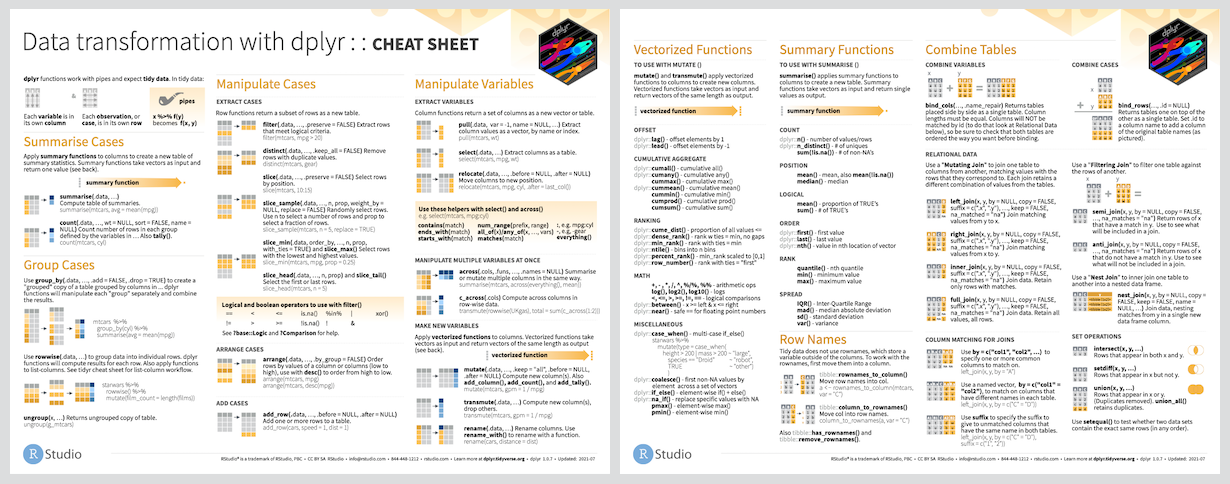
\includegraphics[keepaspectratio]{manipulation/ressources/dplyr-cheatsheet-thumbs.png}}}

\section{webin-R}\label{webin-r-3}

On pourra également se référer au webin-R \#04 (\emph{manipuler les
données avec dplyr}) sur \href{https://youtu.be/aFvBhgmawcs}{YouTube}.

\url{https://youtu.be/aFvBhgmawcs}

\chapter{\texorpdfstring{Facteurs et
\texttt{forcats}}{Facteurs et forcats}}\label{sec-facteurs}

Dans \textbf{R}, les facteurs sont utilisés pour représenter des
variables catégorielles, c'est-à-dire des variables qui ont un nombre
fixé et limité de valeurs possibles (par exemple une variable
\emph{sexe} ou une variable \emph{niveau d'éducation}).

De telles variables sont parfois représentées sous forme textuelle
(vecteurs de type \texttt{character}). Cependant, cela ne permets pas
d'indiquer un ordre spécifique aux modalités, à la différence des
facteurs.

\begin{tcolorbox}[enhanced jigsaw, toptitle=1mm, bottomtitle=1mm, colframe=quarto-callout-note-color-frame, toprule=.15mm, left=2mm, bottomrule=.15mm, opacitybacktitle=0.6, opacityback=0, coltitle=black, breakable, rightrule=.15mm, arc=.35mm, title=\textcolor{quarto-callout-note-color}{\faInfo}\hspace{0.5em}{Note}, colbacktitle=quarto-callout-note-color!10!white, titlerule=0mm, leftrule=.75mm, colback=white]

Lorsque l'on importe des données d'enquêtes, il est fréquent que les
variables catégorielles sont codées sous la forme d'un code numérique
(par exemple 1 pour \emph{femme} et 2 pour \emph{homme}) auquel est
associé une \emph{étiquette de valeur}. C'est notamment le
fonctionnement usuel de logiciels tels que \textbf{SPSS}, \textbf{Stata}
ou \textbf{SAS}. Les étiquettes de valeurs seront abordés dans un
prochain chapitre (voir Chapitre~\ref{sec-etiquettes-valeurs}).

Au moment de l'analyse (tableaux statistiques, graphiques, modèles de
régression\ldots), il sera nécessaire de transformer ces vecteurs avec
étiquettes en facteurs.

\end{tcolorbox}

\section{Création d'un facteur}\label{cruxe9ation-dun-facteur}

Le plus simple pour créer un facteur est de partir d'un vecteur textuel
et d'utiliser la fonction \texttt{factor()}.

\begin{Shaded}
\begin{Highlighting}[]
\NormalTok{x }\OtherTok{\textless{}{-}} \FunctionTok{c}\NormalTok{(}\StringTok{"nord"}\NormalTok{, }\StringTok{"sud"}\NormalTok{, }\StringTok{"sud"}\NormalTok{, }\StringTok{"est"}\NormalTok{, }\StringTok{"est"}\NormalTok{, }\StringTok{"est"}\NormalTok{)}
\NormalTok{x }\SpecialCharTok{|\textgreater{}} 
  \FunctionTok{factor}\NormalTok{()}
\end{Highlighting}
\end{Shaded}

\begin{verbatim}
[1] nord sud  sud  est  est  est 
Levels: est nord sud
\end{verbatim}

Par défaut, les niveaux du facteur obtenu correspondent aux valeurs
uniques du facteur textuel, triés par ordre alphabétique. Si l'on veut
contrôler l'ordre des niveaux, et éventuellement indiquer un niveau
absent des données, on utilisera l'argument \texttt{levels} de
\texttt{factor()}.

\begin{Shaded}
\begin{Highlighting}[]
\NormalTok{x }\SpecialCharTok{|\textgreater{}} 
  \FunctionTok{factor}\NormalTok{(}\AttributeTok{levels =} \FunctionTok{c}\NormalTok{(}\StringTok{"nord"}\NormalTok{, }\StringTok{"est"}\NormalTok{, }\StringTok{"sud"}\NormalTok{, }\StringTok{"ouest"}\NormalTok{))}
\end{Highlighting}
\end{Shaded}

\begin{verbatim}
[1] nord sud  sud  est  est  est 
Levels: nord est sud ouest
\end{verbatim}

Si une valeur observée dans les données n'est pas indiqué dans
\texttt{levels}, elle sera silencieusement convertie en valeur manquante
(\texttt{NA}).

\begin{Shaded}
\begin{Highlighting}[]
\NormalTok{x }\SpecialCharTok{|\textgreater{}} 
  \FunctionTok{factor}\NormalTok{(}\AttributeTok{levels =} \FunctionTok{c}\NormalTok{(}\StringTok{"nord"}\NormalTok{, }\StringTok{"sud"}\NormalTok{))}
\end{Highlighting}
\end{Shaded}

\begin{verbatim}
[1] nord sud  sud  <NA> <NA> <NA>
Levels: nord sud
\end{verbatim}

Si l'on veut être averti par un warning dans ce genre de situation, on
pourra avoir plutôt recours à la fonction
\texttt{readr::parse\_factor()} du package \texttt{\{readr\}}, qui, le
cas échéant, renverra un tableau avec les problèmes rencontrés.

\begin{Shaded}
\begin{Highlighting}[]
\NormalTok{x }\SpecialCharTok{|\textgreater{}} 
\NormalTok{  readr}\SpecialCharTok{::}\FunctionTok{parse\_factor}\NormalTok{(}\AttributeTok{levels =} \FunctionTok{c}\NormalTok{(}\StringTok{"nord"}\NormalTok{, }\StringTok{"sud"}\NormalTok{))}
\end{Highlighting}
\end{Shaded}

\begin{verbatim}
Warning: 3 parsing failures.
row col           expected actual
  4  -- value in level set    est
  5  -- value in level set    est
  6  -- value in level set    est
\end{verbatim}

\begin{verbatim}
[1] nord sud  sud  <NA> <NA> <NA>
attr(,"problems")
# A tibble: 3 x 4
    row   col expected           actual
  <int> <int> <chr>              <chr> 
1     4    NA value in level set est   
2     5    NA value in level set est   
3     6    NA value in level set est   
Levels: nord sud
\end{verbatim}

Une fois un facteur créé, on peut accéder à la liste de ses étiquettes
avec \texttt{levels()}.

\begin{Shaded}
\begin{Highlighting}[]
\NormalTok{f }\OtherTok{\textless{}{-}} \FunctionTok{factor}\NormalTok{(x)}
\FunctionTok{levels}\NormalTok{(f)}
\end{Highlighting}
\end{Shaded}

\begin{verbatim}
[1] "est"  "nord" "sud" 
\end{verbatim}

Dans certaines situations (par exemple pour la réalisation d'une
régression logistique ordinale), on peut avoir avoir besoin d'indiquer
que les modalités du facteur sont ordonnées hiérarchiquement. Dans ce
cas là, on aura simplement recours à \texttt{ordered()} pour
créer/convertir notre facteur.

\begin{Shaded}
\begin{Highlighting}[]
\FunctionTok{c}\NormalTok{(}\StringTok{"supérieur"}\NormalTok{, }\StringTok{"primaire"}\NormalTok{, }\StringTok{"secondaire"}\NormalTok{, }\StringTok{"primaire"}\NormalTok{, }\StringTok{"supérieur"}\NormalTok{) }\SpecialCharTok{|\textgreater{}} 
  \FunctionTok{ordered}\NormalTok{(}\AttributeTok{levels =} \FunctionTok{c}\NormalTok{(}\StringTok{"primaire"}\NormalTok{, }\StringTok{"secondaire"}\NormalTok{, }\StringTok{"supérieur"}\NormalTok{))}
\end{Highlighting}
\end{Shaded}

\begin{verbatim}
[1] supérieur  primaire   secondaire primaire   supérieur 
Levels: primaire < secondaire < supérieur
\end{verbatim}

Techniquement, les valeurs d'un facteur sont stockés de manière interne
à l'aide de nombres entiers, dont la valeur représente la position de
l'étiquette correspondante dans l'attribut \texttt{levels}. Ainsi, un
facteur à \texttt{n} modalités sera toujours codé avec les nombre
entiers allant de 1 à \texttt{n}.

\begin{Shaded}
\begin{Highlighting}[]
\FunctionTok{class}\NormalTok{(f)}
\end{Highlighting}
\end{Shaded}

\begin{verbatim}
[1] "factor"
\end{verbatim}

\begin{Shaded}
\begin{Highlighting}[]
\FunctionTok{typeof}\NormalTok{(f)}
\end{Highlighting}
\end{Shaded}

\begin{verbatim}
[1] "integer"
\end{verbatim}

\begin{Shaded}
\begin{Highlighting}[]
\FunctionTok{as.integer}\NormalTok{(f)}
\end{Highlighting}
\end{Shaded}

\begin{verbatim}
[1] 2 3 3 1 1 1
\end{verbatim}

\begin{Shaded}
\begin{Highlighting}[]
\FunctionTok{as.character}\NormalTok{(f)}
\end{Highlighting}
\end{Shaded}

\begin{verbatim}
[1] "nord" "sud"  "sud"  "est"  "est"  "est" 
\end{verbatim}

\section{Changer l'ordre des
modalités}\label{changer-lordre-des-modalituxe9s}

Le package \texttt{\{forcats\}}, chargé par défaut lorsque l'on exécute
la commande \texttt{library(tidyverse)}, fournie plusieurs fonctions
pour manipuler des facteurs. Pour donner des exemples d'utilisation de
ces différentes fonctions, nous allons utiliser le jeu de données
\texttt{hdv2003} du package \texttt{\{questionr\}}.

\begin{Shaded}
\begin{Highlighting}[]
\FunctionTok{library}\NormalTok{(tidyverse)}
\FunctionTok{data}\NormalTok{(}\StringTok{"hdv2003"}\NormalTok{, }\AttributeTok{package =} \StringTok{"questionr"}\NormalTok{)}
\end{Highlighting}
\end{Shaded}

Considérons la variable \emph{qualif} qui indique le niveau de
qualification des enquêtés. On peut voir la liste des niveaux de ce
facteur, et leur ordre, avec \texttt{levels()}, ou en effectuant un tri
à plat avec la fonction \texttt{questionr::freq()}.

\begin{Shaded}
\begin{Highlighting}[]
\NormalTok{hdv2003}\SpecialCharTok{$}\NormalTok{qualif }\SpecialCharTok{|\textgreater{}} \FunctionTok{levels}\NormalTok{()}
\end{Highlighting}
\end{Shaded}

\begin{verbatim}
[1] "Ouvrier specialise"       "Ouvrier qualifie"        
[3] "Technicien"               "Profession intermediaire"
[5] "Cadre"                    "Employe"                 
[7] "Autre"                   
\end{verbatim}

\begin{Shaded}
\begin{Highlighting}[]
\NormalTok{hdv2003 }\SpecialCharTok{|\textgreater{}}\NormalTok{ guideR}\SpecialCharTok{::}\FunctionTok{proportion}\NormalTok{(qualif)}
\end{Highlighting}
\end{Shaded}

\begin{verbatim}
# A tibble: 8 x 4
  qualif                       n     N  prop
  <fct>                    <int> <int> <dbl>
1 Ouvrier specialise         203  2000  10.2
2 Ouvrier qualifie           292  2000  14.6
3 Technicien                  86  2000   4.3
4 Profession intermediaire   160  2000   8  
5 Cadre                      260  2000  13  
6 Employe                    594  2000  29.7
7 Autre                       58  2000   2.9
8 <NA>                       347  2000  17.3
\end{verbatim}

Parfois, on a simplement besoin d'inverser l'ordre des facteurs, ce qui
peut se faire facilement avec la fonction \texttt{forcats::fct\_rev()}.
Elle renvoie le facteur fourni en entrée en ayant inverser l'ordre des
modalités (mais sans modifier l'ordre des valeurs dans le vecteur).

\begin{Shaded}
\begin{Highlighting}[]
\NormalTok{hdv2003 }\SpecialCharTok{|\textgreater{}}\NormalTok{ guideR}\SpecialCharTok{::}\FunctionTok{proportion}\NormalTok{(qualif }\SpecialCharTok{|\textgreater{}} \FunctionTok{fct\_rev}\NormalTok{())}
\end{Highlighting}
\end{Shaded}

\begin{verbatim}
# A tibble: 8 x 4
  `fct_rev(qualif)`            n     N  prop
  <fct>                    <int> <int> <dbl>
1 Autre                       58  2000   2.9
2 Employe                    594  2000  29.7
3 Cadre                      260  2000  13  
4 Profession intermediaire   160  2000   8  
5 Technicien                  86  2000   4.3
6 Ouvrier qualifie           292  2000  14.6
7 Ouvrier specialise         203  2000  10.2
8 <NA>                       347  2000  17.3
\end{verbatim}

Pour plus de contrôle, on utilisera \texttt{forcats::fct\_relevel()} où
l'on indique l'ordre souhaité des modalités. On peut également seulement
indiquer les premières modalités, les autres seront ajoutées à la fin
sans changer leur ordre.

\begin{Shaded}
\begin{Highlighting}[]
\NormalTok{hdv2003 }\SpecialCharTok{|\textgreater{}} 
\NormalTok{  guideR}\SpecialCharTok{::}\FunctionTok{proportion}\NormalTok{(}
\NormalTok{    qualif }\SpecialCharTok{|\textgreater{}} \FunctionTok{fct\_relevel}\NormalTok{(}\StringTok{"Cadre"}\NormalTok{, }\StringTok{"Autre"}\NormalTok{, }\StringTok{"Technicien"}\NormalTok{, }\StringTok{"Employe"}\NormalTok{)}
\NormalTok{  )}
\end{Highlighting}
\end{Shaded}

\begin{verbatim}
# A tibble: 8 x 4
  fct_relevel(qualif, "Cadre", "Autre", "Technicien", "Emplo~1     n     N  prop
  <fct>                                                        <int> <int> <dbl>
1 Cadre                                                          260  2000  13  
2 Autre                                                           58  2000   2.9
3 Technicien                                                      86  2000   4.3
4 Employe                                                        594  2000  29.7
5 Ouvrier specialise                                             203  2000  10.2
6 Ouvrier qualifie                                               292  2000  14.6
7 Profession intermediaire                                       160  2000   8  
8 <NA>                                                           347  2000  17.3
# i abbreviated name:
#   1: `fct_relevel(qualif, "Cadre", "Autre", "Technicien", "Employe")`
\end{verbatim}

La fonction \texttt{forcats::fct\_infreq()} ordonne les modalités de
celle la plus fréquente à celle la moins fréquente (nombre
d'observations)~:

\begin{Shaded}
\begin{Highlighting}[]
\NormalTok{hdv2003 }\SpecialCharTok{|\textgreater{}}\NormalTok{ guideR}\SpecialCharTok{::}\FunctionTok{proportion}\NormalTok{(}\FunctionTok{fct\_infreq}\NormalTok{(qualif))}
\end{Highlighting}
\end{Shaded}

\begin{verbatim}
# A tibble: 8 x 4
  `fct_infreq(qualif)`         n     N  prop
  <fct>                    <int> <int> <dbl>
1 Employe                    594  2000  29.7
2 Ouvrier qualifie           292  2000  14.6
3 Cadre                      260  2000  13  
4 Ouvrier specialise         203  2000  10.2
5 Profession intermediaire   160  2000   8  
6 Technicien                  86  2000   4.3
7 Autre                       58  2000   2.9
8 <NA>                       347  2000  17.3
\end{verbatim}

Pour inverser l'ordre, on combinera \texttt{forcats::fct\_infreq()} avec
\texttt{forcats::fct\_rev()}.

\begin{Shaded}
\begin{Highlighting}[]
\NormalTok{hdv2003 }\SpecialCharTok{|\textgreater{}}\NormalTok{ guideR}\SpecialCharTok{::}\FunctionTok{proportion}\NormalTok{(qualif }\SpecialCharTok{|\textgreater{}} \FunctionTok{fct\_infreq}\NormalTok{() }\SpecialCharTok{|\textgreater{}} \FunctionTok{fct\_rev}\NormalTok{())}
\end{Highlighting}
\end{Shaded}

\begin{verbatim}
# A tibble: 8 x 4
  `fct_rev(fct_infreq(qualif))`     n     N  prop
  <fct>                         <int> <int> <dbl>
1 Autre                            58  2000   2.9
2 Technicien                       86  2000   4.3
3 Profession intermediaire        160  2000   8  
4 Ouvrier specialise              203  2000  10.2
5 Cadre                           260  2000  13  
6 Ouvrier qualifie                292  2000  14.6
7 Employe                         594  2000  29.7
8 <NA>                            347  2000  17.3
\end{verbatim}

Dans certains cas, on souhaite créer un facteur dont les modalités sont
triées selon leur ordre d'apparition dans le jeu de données. Pour cela,
on aura recours à \texttt{forcats::fct\_inorder()}.

\begin{Shaded}
\begin{Highlighting}[]
\NormalTok{v }\OtherTok{\textless{}{-}} \FunctionTok{c}\NormalTok{(}\StringTok{"c"}\NormalTok{, }\StringTok{"a"}\NormalTok{, }\StringTok{"d"}\NormalTok{, }\StringTok{"b"}\NormalTok{, }\StringTok{"a"}\NormalTok{, }\StringTok{"c"}\NormalTok{)}
\FunctionTok{factor}\NormalTok{(v)}
\end{Highlighting}
\end{Shaded}

\begin{verbatim}
[1] c a d b a c
Levels: a b c d
\end{verbatim}

\begin{Shaded}
\begin{Highlighting}[]
\FunctionTok{fct\_inorder}\NormalTok{(v)}
\end{Highlighting}
\end{Shaded}

\begin{verbatim}
[1] c a d b a c
Levels: c a d b
\end{verbatim}

La fonction \texttt{forcats::fct\_reorder()} permets de trier les
modalités en fonction d'une autre variable. Par exemple, si je souhaite
trier les modalités de la variable \emph{qualif} en fonction de l'âge
moyen (dans chaque modalité)~:

\begin{Shaded}
\begin{Highlighting}[]
\NormalTok{hdv2003}\SpecialCharTok{$}\NormalTok{qualif\_tri\_age }\OtherTok{\textless{}{-}}
\NormalTok{  hdv2003}\SpecialCharTok{$}\NormalTok{qualif }\SpecialCharTok{|\textgreater{}} 
  \FunctionTok{fct\_reorder}\NormalTok{(hdv2003}\SpecialCharTok{$}\NormalTok{age, }\AttributeTok{.fun =}\NormalTok{ mean)}
\NormalTok{hdv2003 }\SpecialCharTok{|\textgreater{}} 
\NormalTok{  dplyr}\SpecialCharTok{::}\FunctionTok{group\_by}\NormalTok{(qualif\_tri\_age) }\SpecialCharTok{|\textgreater{}} 
\NormalTok{  dplyr}\SpecialCharTok{::}\FunctionTok{summarise}\NormalTok{(}\AttributeTok{age\_moyen =} \FunctionTok{mean}\NormalTok{(age))}
\end{Highlighting}
\end{Shaded}

\begin{verbatim}
# A tibble: 8 x 2
  qualif_tri_age           age_moyen
  <fct>                        <dbl>
1 Technicien                    45.9
2 Employe                       46.7
3 Autre                         47.0
4 Ouvrier specialise            48.9
5 Profession intermediaire      49.1
6 Cadre                         49.7
7 Ouvrier qualifie              50.0
8 <NA>                          47.9
\end{verbatim}

\begin{tcolorbox}[enhanced jigsaw, toptitle=1mm, bottomtitle=1mm, colframe=quarto-callout-tip-color-frame, toprule=.15mm, left=2mm, bottomrule=.15mm, opacitybacktitle=0.6, opacityback=0, coltitle=black, breakable, rightrule=.15mm, arc=.35mm, title=\textcolor{quarto-callout-tip-color}{\faLightbulb}\hspace{0.5em}{Astuce}, colbacktitle=quarto-callout-tip-color!10!white, titlerule=0mm, leftrule=.75mm, colback=white]

\texttt{\{questionr\}} propose une interface graphique afin de faciliter
les opérations de ré-ordonnancement manuel. Pour la lancer, sélectionner
le menu \emph{Addins} puis \emph{Levels ordering}, ou exécuter la
fonction \texttt{questionr::iorder()} en lui passant comme paramètre le
facteur à réordonner.

\pandocbounded{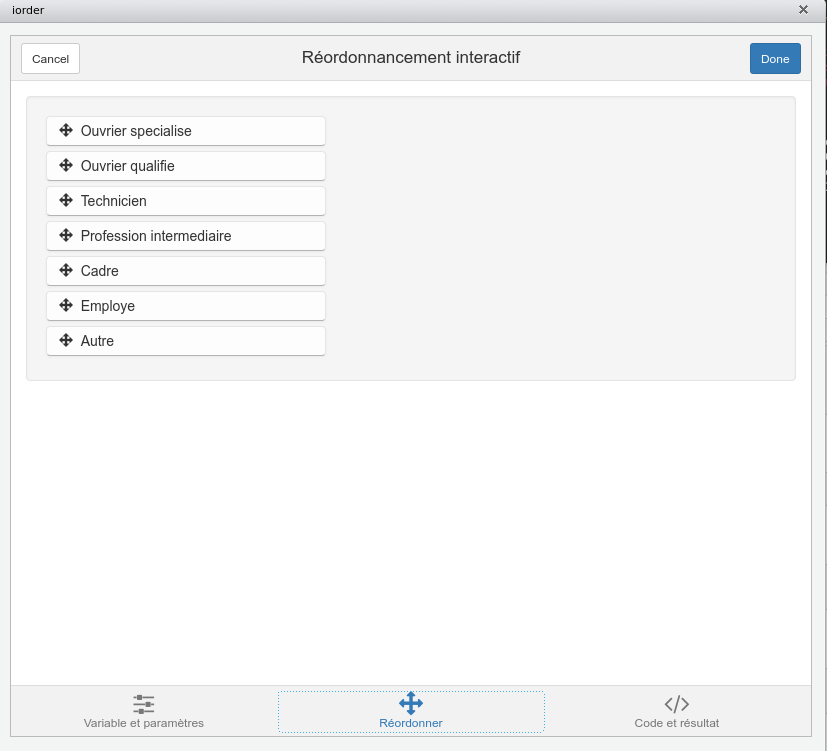
\includegraphics[keepaspectratio]{manipulation/ressources/iorder.png}}

Une démonstration en vidéo de cet \emph{add-in} est disponible dans le
webin-R \#05 (\emph{recoder des variables}) sur
{[}YouTube{]}(https://youtu.be/CokvTbtWdwc?t=3934).

\url{https://youtu.be/CokvTbtWdwc}

\end{tcolorbox}

\section{Modifier les modalités}\label{sec-modifier-modalites}

Pour modifier le nom des modalités, on pourra avoir recours à
\texttt{forcats::fct\_recode()} avec une syntaxe de la forme
\texttt{"nouveau\ nom"\ =\ "ancien\ nom"}.

\begin{Shaded}
\begin{Highlighting}[]
\NormalTok{hdv2003 }\SpecialCharTok{|\textgreater{}}\NormalTok{ guideR}\SpecialCharTok{::}\FunctionTok{proportion}\NormalTok{(sexe)}
\end{Highlighting}
\end{Shaded}

\begin{verbatim}
# A tibble: 2 x 4
  sexe      n     N  prop
  <fct> <int> <int> <dbl>
1 Homme   899  2000  45.0
2 Femme  1101  2000  55.0
\end{verbatim}

\begin{Shaded}
\begin{Highlighting}[]
\NormalTok{hdv2003}\SpecialCharTok{$}\NormalTok{sexe }\OtherTok{\textless{}{-}} 
\NormalTok{  hdv2003}\SpecialCharTok{$}\NormalTok{sexe }\SpecialCharTok{|\textgreater{}} 
  \FunctionTok{fct\_recode}\NormalTok{(}\AttributeTok{f =} \StringTok{"Femme"}\NormalTok{, }\AttributeTok{m =} \StringTok{"Homme"}\NormalTok{)}
\NormalTok{hdv2003 }\SpecialCharTok{|\textgreater{}}\NormalTok{ guideR}\SpecialCharTok{::}\FunctionTok{proportion}\NormalTok{(sexe)}
\end{Highlighting}
\end{Shaded}

\begin{verbatim}
# A tibble: 2 x 4
  sexe      n     N  prop
  <fct> <int> <int> <dbl>
1 m       899  2000  45.0
2 f      1101  2000  55.0
\end{verbatim}

On peut également fusionner des modalités ensemble en leur attribuant le
même nom.

\begin{Shaded}
\begin{Highlighting}[]
\NormalTok{hdv2003 }\SpecialCharTok{|\textgreater{}}\NormalTok{ guideR}\SpecialCharTok{::}\FunctionTok{proportion}\NormalTok{(nivetud)}
\end{Highlighting}
\end{Shaded}

\begin{verbatim}
# A tibble: 9 x 4
  nivetud                                                          n     N  prop
  <fct>                                                        <int> <int> <dbl>
1 N'a jamais fait d'etudes                                        39  2000  1.95
2 A arrete ses etudes, avant la derniere annee d'etudes prima~    86  2000  4.3 
3 Derniere annee d'etudes primaires                              341  2000 17.0 
4 1er cycle                                                      204  2000 10.2 
5 2eme cycle                                                     183  2000  9.15
6 Enseignement technique ou professionnel court                  463  2000 23.2 
7 Enseignement technique ou professionnel long                   131  2000  6.55
8 Enseignement superieur y compris technique superieur           441  2000 22.0 
9 <NA>                                                           112  2000  5.6 
\end{verbatim}

\begin{Shaded}
\begin{Highlighting}[]
\NormalTok{hdv2003}\SpecialCharTok{$}\NormalTok{instruction }\OtherTok{\textless{}{-}} 
\NormalTok{  hdv2003}\SpecialCharTok{$}\NormalTok{nivetud }\SpecialCharTok{|\textgreater{}} 
  \FunctionTok{fct\_recode}\NormalTok{(}
    \StringTok{"primaire"} \OtherTok{=} \StringTok{"N\textquotesingle{}a jamais fait d\textquotesingle{}etudes"}\NormalTok{,}
    \StringTok{"primaire"} \OtherTok{=} \StringTok{"A arrete ses etudes, avant la derniere annee d\textquotesingle{}etudes primaires"}\NormalTok{,}
    \StringTok{"primaire"} \OtherTok{=} \StringTok{"Derniere annee d\textquotesingle{}etudes primaires"}\NormalTok{,}
    \StringTok{"secondaire"} \OtherTok{=} \StringTok{"1er cycle"}\NormalTok{,}
    \StringTok{"secondaire"} \OtherTok{=} \StringTok{"2eme cycle"}\NormalTok{,}
    \StringTok{"technique/professionnel"} \OtherTok{=} \StringTok{"Enseignement technique ou professionnel court"}\NormalTok{,}
    \StringTok{"technique/professionnel"} \OtherTok{=} \StringTok{"Enseignement technique ou professionnel long"}\NormalTok{,}
    \StringTok{"supérieur"} \OtherTok{=} \StringTok{"Enseignement superieur y compris technique superieur"}
\NormalTok{  )}
\NormalTok{hdv2003 }\SpecialCharTok{|\textgreater{}}\NormalTok{ guideR}\SpecialCharTok{::}\FunctionTok{proportion}\NormalTok{(instruction)}
\end{Highlighting}
\end{Shaded}

\begin{verbatim}
# A tibble: 5 x 4
  instruction                 n     N  prop
  <fct>                   <int> <int> <dbl>
1 primaire                  466  2000  23.3
2 secondaire                387  2000  19.4
3 technique/professionnel   594  2000  29.7
4 supérieur                 441  2000  22.0
5 <NA>                      112  2000   5.6
\end{verbatim}

\begin{tcolorbox}[enhanced jigsaw, toptitle=1mm, bottomtitle=1mm, colframe=quarto-callout-tip-color-frame, toprule=.15mm, left=2mm, bottomrule=.15mm, opacitybacktitle=0.6, opacityback=0, coltitle=black, breakable, rightrule=.15mm, arc=.35mm, title=\textcolor{quarto-callout-tip-color}{\faLightbulb}\hspace{0.5em}{Interface graphique}, colbacktitle=quarto-callout-tip-color!10!white, titlerule=0mm, leftrule=.75mm, colback=white]

Le package\texttt{\{questionr\}} propose une interface graphique
facilitant le recodage des modalités d'une variable qualitative.
L'objectif est de permettre à la personne qui l'utilise de saisir les
nouvelles valeurs dans un formulaire, et de générer ensuite le code R
correspondant au recodage indiqué.

Pour utiliser cette interface, sous \textbf{RStudio} vous pouvez aller
dans le menu \emph{Addins} (présent dans la barre d'outils principale)
puis choisir \emph{Levels recoding}. Sinon, vous pouvez lancer dans la
console la fonction \texttt{questionr::irec()} en lui passant comme
paramètre la variable à recoder.

\pandocbounded{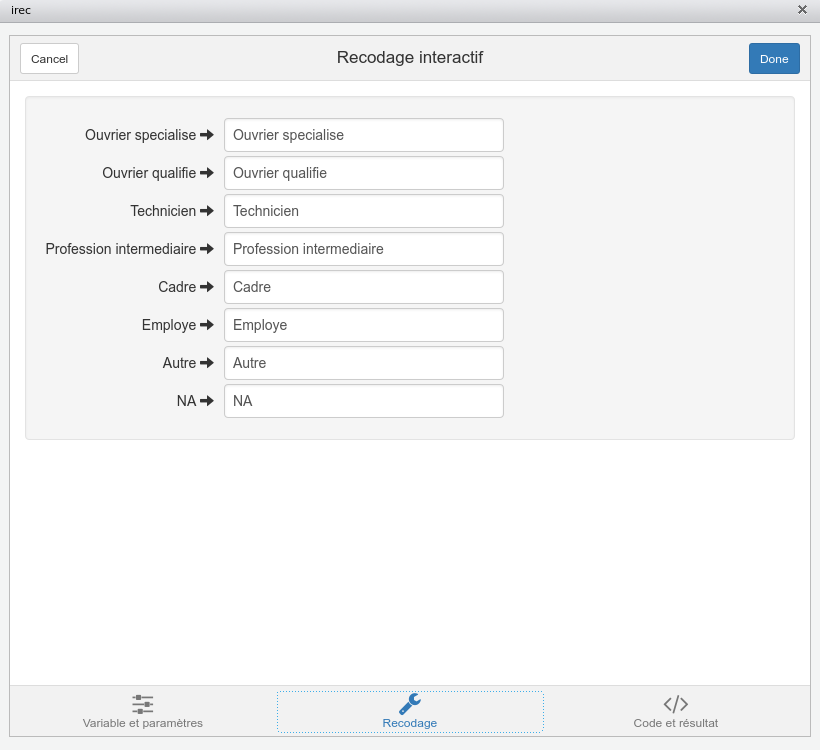
\includegraphics[keepaspectratio]{manipulation/ressources/irec.png}}

Une démonstration en vidéo de cet \emph{add-in} est disponible dans le
webin-R \#05 (\emph{recoder des variables}) sur
{[}YouTube{]}(https://youtu.be/CokvTbtWdwc?t=3387).

\url{https://youtu.be/CokvTbtWdwc}

\end{tcolorbox}

La fonction \texttt{forcats::fct\_collapse()} est une variante de
\texttt{forcats::fct\_recode()} pour indiquer les fusions de modalités.
La même recodification s'écrirait alors~:

\begin{Shaded}
\begin{Highlighting}[]
\NormalTok{hdv2003}\SpecialCharTok{$}\NormalTok{instruction }\OtherTok{\textless{}{-}} 
\NormalTok{  hdv2003}\SpecialCharTok{$}\NormalTok{nivetud }\SpecialCharTok{|\textgreater{}} 
  \FunctionTok{fct\_collapse}\NormalTok{(}
    \StringTok{"primaire"} \OtherTok{=} \FunctionTok{c}\NormalTok{(}
      \StringTok{"N\textquotesingle{}a jamais fait d\textquotesingle{}etudes"}\NormalTok{,}
      \StringTok{"A arrete ses etudes, avant la derniere annee d\textquotesingle{}etudes primaires"}\NormalTok{,}
      \StringTok{"Derniere annee d\textquotesingle{}etudes primaires"}
\NormalTok{    ),}
    \StringTok{"secondaire"} \OtherTok{=} \FunctionTok{c}\NormalTok{(}
      \StringTok{"1er cycle"}\NormalTok{,}
      \StringTok{"2eme cycle"}
\NormalTok{    ),}
    \StringTok{"technique/professionnel"} \OtherTok{=} \FunctionTok{c}\NormalTok{(}
      \StringTok{"Enseignement technique ou professionnel court"}\NormalTok{,}
      \StringTok{"Enseignement technique ou professionnel long"}
\NormalTok{    ),}
    \StringTok{"supérieur"} \OtherTok{=} \StringTok{"Enseignement superieur y compris technique superieur"}
\NormalTok{  )}
\end{Highlighting}
\end{Shaded}

Pour transformer les valeurs manquantes (\texttt{NA}) en une modalité
explicite, on pourra avoir recours à
\texttt{forcats::fct\_na\_value\_to\_level()}\footnote{Cette fonction
  s'appelait précédemment \texttt{forcats::fct\_explicit\_na()} et a été
  renommée depuis la version 1.0.0 de \texttt{\{forcats\}.}}.

\begin{Shaded}
\begin{Highlighting}[]
\NormalTok{hdv2003}\SpecialCharTok{$}\NormalTok{instruction }\OtherTok{\textless{}{-}}
\NormalTok{  hdv2003}\SpecialCharTok{$}\NormalTok{instruction }\SpecialCharTok{|\textgreater{}} 
  \FunctionTok{fct\_na\_value\_to\_level}\NormalTok{(}\AttributeTok{level =} \StringTok{"(manquant)"}\NormalTok{)}
\NormalTok{hdv2003 }\SpecialCharTok{|\textgreater{}}\NormalTok{ guideR}\SpecialCharTok{::}\FunctionTok{proportion}\NormalTok{(instruction)}
\end{Highlighting}
\end{Shaded}

\begin{verbatim}
# A tibble: 5 x 4
  instruction                 n     N  prop
  <fct>                   <int> <int> <dbl>
1 primaire                  466  2000  23.3
2 secondaire                387  2000  19.4
3 technique/professionnel   594  2000  29.7
4 supérieur                 441  2000  22.0
5 (manquant)                112  2000   5.6
\end{verbatim}

Plusieurs fonctions permettent de regrouper plusieurs modalités dans une
modalité \emph{autres}.

Par exemple, avec \texttt{forcats::fct\_other()}, on pourra indiquer les
modalités à garder.

\begin{Shaded}
\begin{Highlighting}[]
\NormalTok{hdv2003 }\SpecialCharTok{|\textgreater{}}\NormalTok{ guideR}\SpecialCharTok{::}\FunctionTok{proportion}\NormalTok{(qualif)}
\end{Highlighting}
\end{Shaded}

\begin{verbatim}
# A tibble: 8 x 4
  qualif                       n     N  prop
  <fct>                    <int> <int> <dbl>
1 Ouvrier specialise         203  2000  10.2
2 Ouvrier qualifie           292  2000  14.6
3 Technicien                  86  2000   4.3
4 Profession intermediaire   160  2000   8  
5 Cadre                      260  2000  13  
6 Employe                    594  2000  29.7
7 Autre                       58  2000   2.9
8 <NA>                       347  2000  17.3
\end{verbatim}

\begin{Shaded}
\begin{Highlighting}[]
\NormalTok{hdv2003 }\SpecialCharTok{|\textgreater{}} 
\NormalTok{  guideR}\SpecialCharTok{::}\FunctionTok{proportion}\NormalTok{(}
\NormalTok{    qualif }\SpecialCharTok{|\textgreater{}} \FunctionTok{fct\_other}\NormalTok{(}\AttributeTok{keep =} \FunctionTok{c}\NormalTok{(}\StringTok{"Technicien"}\NormalTok{, }\StringTok{"Cadre"}\NormalTok{, }\StringTok{"Employe"}\NormalTok{))}
\NormalTok{  )}
\end{Highlighting}
\end{Shaded}

\begin{verbatim}
# A tibble: 5 x 4
  fct_other(qualif, keep = c("Technicien", "Cadre", "Employe~1     n     N  prop
  <fct>                                                        <int> <int> <dbl>
1 Technicien                                                      86  2000   4.3
2 Cadre                                                          260  2000  13  
3 Employe                                                        594  2000  29.7
4 Other                                                          713  2000  35.6
5 <NA>                                                           347  2000  17.3
# i abbreviated name:
#   1: `fct_other(qualif, keep = c("Technicien", "Cadre", "Employe"))`
\end{verbatim}

La fonction \texttt{forcats::fct\_lump\_n()} permets de ne conserver que
les modalités les plus fréquentes et de regrouper les autres dans une
modalité \emph{autres}.

\begin{Shaded}
\begin{Highlighting}[]
\NormalTok{hdv2003 }\SpecialCharTok{|\textgreater{}} 
\NormalTok{  guideR}\SpecialCharTok{::}\FunctionTok{proportion}\NormalTok{(}
\NormalTok{    qualif }\SpecialCharTok{|\textgreater{}} \FunctionTok{fct\_lump\_n}\NormalTok{(}\AttributeTok{n =} \DecValTok{4}\NormalTok{, }\AttributeTok{other\_level =} \StringTok{"Autres"}\NormalTok{)}
\NormalTok{  )}
\end{Highlighting}
\end{Shaded}

\begin{verbatim}
# A tibble: 6 x 4
  `fct_lump_n(qualif, n = 4, other_level = "Autres")`     n     N  prop
  <fct>                                               <int> <int> <dbl>
1 Ouvrier specialise                                    203  2000  10.2
2 Ouvrier qualifie                                      292  2000  14.6
3 Cadre                                                 260  2000  13  
4 Employe                                               594  2000  29.7
5 Autres                                                304  2000  15.2
6 <NA>                                                  347  2000  17.3
\end{verbatim}

Et \texttt{forcats::fct\_lump\_min()} celles qui ont un minimum
d'observations.

\begin{Shaded}
\begin{Highlighting}[]
\NormalTok{hdv2003 }\SpecialCharTok{|\textgreater{}} 
\NormalTok{  guideR}\SpecialCharTok{::}\FunctionTok{proportion}\NormalTok{(}
\NormalTok{    qualif }\SpecialCharTok{|\textgreater{}} \FunctionTok{fct\_lump\_min}\NormalTok{(}\AttributeTok{min =} \DecValTok{200}\NormalTok{, }\AttributeTok{other\_level =} \StringTok{"Autres"}\NormalTok{)}
\NormalTok{  )}
\end{Highlighting}
\end{Shaded}

\begin{verbatim}
# A tibble: 6 x 4
  `fct_lump_min(qualif, min = 200, other_level = "Autres")`     n     N  prop
  <fct>                                                     <int> <int> <dbl>
1 Ouvrier specialise                                          203  2000  10.2
2 Ouvrier qualifie                                            292  2000  14.6
3 Cadre                                                       260  2000  13  
4 Employe                                                     594  2000  29.7
5 Autres                                                      304  2000  15.2
6 <NA>                                                        347  2000  17.3
\end{verbatim}

Il peut arriver qu'une des modalités d'un facteur ne soit pas
représentée dans les données.

\begin{Shaded}
\begin{Highlighting}[]
\NormalTok{v }\OtherTok{\textless{}{-}} \FunctionTok{factor}\NormalTok{(}
  \FunctionTok{c}\NormalTok{(}\StringTok{"a"}\NormalTok{, }\StringTok{"a"}\NormalTok{, }\StringTok{"b"}\NormalTok{, }\StringTok{"a"}\NormalTok{),}
  \AttributeTok{levels =} \FunctionTok{c}\NormalTok{(}\StringTok{"a"}\NormalTok{, }\StringTok{"b"}\NormalTok{, }\StringTok{"c"}\NormalTok{)}
\NormalTok{)}
\NormalTok{questionr}\SpecialCharTok{::}\FunctionTok{freq}\NormalTok{(v)}
\end{Highlighting}
\end{Shaded}

\begin{verbatim}
  n  % val%
a 3 75   75
b 1 25   25
c 0  0    0
\end{verbatim}

Pour calculer certains tests statistiques ou faire tourner un modèle,
ces modalités sans observation peuvent être problématiques.
\texttt{forcats::fct\_drop()} permet de supprimer les modalités qui
n'apparaissent pas dans les données.

\begin{Shaded}
\begin{Highlighting}[]
\NormalTok{v}
\end{Highlighting}
\end{Shaded}

\begin{verbatim}
[1] a a b a
Levels: a b c
\end{verbatim}

\begin{Shaded}
\begin{Highlighting}[]
\NormalTok{v }\SpecialCharTok{|\textgreater{}} \FunctionTok{fct\_drop}\NormalTok{()}
\end{Highlighting}
\end{Shaded}

\begin{verbatim}
[1] a a b a
Levels: a b
\end{verbatim}

À l'inverse, \texttt{forcats::fct\_expand()} permet d'ajouter une ou
plusieurs modalités à un facteur.

\begin{Shaded}
\begin{Highlighting}[]
\NormalTok{v}
\end{Highlighting}
\end{Shaded}

\begin{verbatim}
[1] a a b a
Levels: a b c
\end{verbatim}

\begin{Shaded}
\begin{Highlighting}[]
\NormalTok{v }\SpecialCharTok{|\textgreater{}} \FunctionTok{fct\_expand}\NormalTok{(}\StringTok{"d"}\NormalTok{, }\StringTok{"e"}\NormalTok{)}
\end{Highlighting}
\end{Shaded}

\begin{verbatim}
[1] a a b a
Levels: a b c d e
\end{verbatim}

\section{Découper une variable numérique en classes}\label{sec-cut}

Il est fréquent d'avoir besoin de découper une variable numérique en une
variable catégorielles (un facteur) à plusieurs modalités, par exemple
pour créer des groupes d'âges à partir d'une variable \emph{age}.

On utilise pour cela la fonction \texttt{cut()} qui prend, outre la
variable à découper, un certain nombre d'arguments~:

\begin{itemize}
\tightlist
\item
  \texttt{breaks} indique soit le nombre de classes souhaité, soit, si
  on lui fournit un vecteur, les limites des classes~;
\item
  \texttt{labels} permet de modifier les noms de modalités attribués aux
  classes~;
\item
  \texttt{include.lowest} et \texttt{right} influent sur la manière dont
  les valeurs situées à la frontière des classes seront inclues ou
  exclues~;
\item
  \texttt{dig.lab} indique le nombre de chiffres après la virgule à
  conserver dans les noms de modalités.
\end{itemize}

Prenons tout de suite un exemple et tentons de découper la variable
\emph{age} en cinq classes~:

\begin{Shaded}
\begin{Highlighting}[]
\NormalTok{hdv2003 }\OtherTok{\textless{}{-}}
\NormalTok{  hdv2003 }\SpecialCharTok{|\textgreater{}} 
  \FunctionTok{mutate}\NormalTok{(}\AttributeTok{groupe\_ages =} \FunctionTok{cut}\NormalTok{(age, }\DecValTok{5}\NormalTok{))}
\NormalTok{hdv2003 }\SpecialCharTok{|\textgreater{}}\NormalTok{ guideR}\SpecialCharTok{::}\FunctionTok{proportion}\NormalTok{(groupe\_ages)}
\end{Highlighting}
\end{Shaded}

\begin{verbatim}
# A tibble: 5 x 4
  groupe_ages     n     N  prop
  <fct>       <int> <int> <dbl>
1 (17.9,33.8]   454  2000 22.7 
2 (33.8,49.6]   628  2000 31.4 
3 (49.6,65.4]   556  2000 27.8 
4 (65.4,81.2]   319  2000 16.0 
5 (81.2,97.1]    43  2000  2.15
\end{verbatim}

Par défaut \textbf{R} nous a bien créé cinq classes d'amplitudes égales.
La première classe va de 17,9 à 33,8 ans (en fait de 17 à 32), etc.

Les frontières de classe seraient plus présentables si elles utilisaient
des nombres ronds. On va donc spécifier manuellement le découpage
souhaité, par tranches de 20 ans~:

\begin{Shaded}
\begin{Highlighting}[]
\NormalTok{hdv2003 }\OtherTok{\textless{}{-}}
\NormalTok{  hdv2003 }\SpecialCharTok{|\textgreater{}} 
  \FunctionTok{mutate}\NormalTok{(}\AttributeTok{groupe\_ages =} \FunctionTok{cut}\NormalTok{(age, }\FunctionTok{c}\NormalTok{(}\DecValTok{18}\NormalTok{, }\DecValTok{20}\NormalTok{, }\DecValTok{40}\NormalTok{, }\DecValTok{60}\NormalTok{, }\DecValTok{80}\NormalTok{, }\DecValTok{97}\NormalTok{)))}
\NormalTok{hdv2003 }\SpecialCharTok{|\textgreater{}}\NormalTok{ guideR}\SpecialCharTok{::}\FunctionTok{proportion}\NormalTok{(groupe\_ages)}
\end{Highlighting}
\end{Shaded}

\begin{verbatim}
# A tibble: 6 x 4
  groupe_ages     n     N  prop
  <fct>       <int> <int> <dbl>
1 (18,20]        55  2000  2.75
2 (20,40]       660  2000 33   
3 (40,60]       780  2000 39   
4 (60,80]       436  2000 21.8 
5 (80,97]        52  2000  2.6 
6 <NA>           17  2000  0.85
\end{verbatim}

Les symboles dans les noms attribués aux classes ont leur importance~:
\texttt{(} signifie que la frontière de la classe est exclue, tandis que
\texttt{{[}} signifie qu'elle est incluse. Ainsi, \texttt{(20,40{]}}
signifie «~strictement supérieur à 20 et inférieur ou égal à 40~».

On remarque que du coup, dans notre exemple précédent, la valeur
minimale, 18, est exclue de notre première classe, et qu'une observation
est donc absente de ce découpage. Pour résoudre ce problème on peut soit
faire commencer la première classe à 17, soit utiliser l'option
\texttt{include.lowest=TRUE}~:

\begin{Shaded}
\begin{Highlighting}[]
\NormalTok{hdv2003 }\OtherTok{\textless{}{-}}
\NormalTok{  hdv2003 }\SpecialCharTok{|\textgreater{}} 
  \FunctionTok{mutate}\NormalTok{(}\AttributeTok{groupe\_ages =} \FunctionTok{cut}\NormalTok{(}
\NormalTok{    age, }
    \FunctionTok{c}\NormalTok{(}\DecValTok{18}\NormalTok{, }\DecValTok{20}\NormalTok{, }\DecValTok{40}\NormalTok{, }\DecValTok{60}\NormalTok{, }\DecValTok{80}\NormalTok{, }\DecValTok{97}\NormalTok{),}
    \AttributeTok{include.lowest =} \ConstantTok{TRUE}
\NormalTok{  ))}
\NormalTok{hdv2003 }\SpecialCharTok{|\textgreater{}}\NormalTok{ guideR}\SpecialCharTok{::}\FunctionTok{proportion}\NormalTok{(groupe\_ages)}
\end{Highlighting}
\end{Shaded}

\begin{verbatim}
# A tibble: 5 x 4
  groupe_ages     n     N  prop
  <fct>       <int> <int> <dbl>
1 [18,20]        72  2000   3.6
2 (20,40]       660  2000  33  
3 (40,60]       780  2000  39  
4 (60,80]       436  2000  21.8
5 (80,97]        52  2000   2.6
\end{verbatim}

On peut également modifier le sens des intervalles avec l'option
\texttt{right=FALSE}~:

\begin{Shaded}
\begin{Highlighting}[]
\NormalTok{hdv2003 }\OtherTok{\textless{}{-}}
\NormalTok{  hdv2003 }\SpecialCharTok{|\textgreater{}} 
  \FunctionTok{mutate}\NormalTok{(}\AttributeTok{groupe\_ages =} \FunctionTok{cut}\NormalTok{(}
\NormalTok{    age, }
    \FunctionTok{c}\NormalTok{(}\DecValTok{18}\NormalTok{, }\DecValTok{20}\NormalTok{, }\DecValTok{40}\NormalTok{, }\DecValTok{60}\NormalTok{, }\DecValTok{80}\NormalTok{, }\DecValTok{97}\NormalTok{),}
    \AttributeTok{include.lowest =} \ConstantTok{TRUE}\NormalTok{,}
    \AttributeTok{right =} \ConstantTok{FALSE}
\NormalTok{  ))}
\NormalTok{hdv2003 }\SpecialCharTok{|\textgreater{}}\NormalTok{ guideR}\SpecialCharTok{::}\FunctionTok{proportion}\NormalTok{(groupe\_ages)}
\end{Highlighting}
\end{Shaded}

\begin{verbatim}
# A tibble: 5 x 4
  groupe_ages     n     N  prop
  <fct>       <int> <int> <dbl>
1 [18,20)        48  2000   2.4
2 [20,40)       643  2000  32.2
3 [40,60)       793  2000  39.6
4 [60,80)       454  2000  22.7
5 [80,97]        62  2000   3.1
\end{verbatim}

\begin{tcolorbox}[enhanced jigsaw, toptitle=1mm, bottomtitle=1mm, colframe=quarto-callout-tip-color-frame, toprule=.15mm, left=2mm, bottomrule=.15mm, opacitybacktitle=0.6, opacityback=0, coltitle=black, breakable, rightrule=.15mm, arc=.35mm, title=\textcolor{quarto-callout-tip-color}{\faLightbulb}\hspace{0.5em}{Interface graphique}, colbacktitle=quarto-callout-tip-color!10!white, titlerule=0mm, leftrule=.75mm, colback=white]

Il n'est pas nécessaire de connaître toutes les options de
\texttt{cut()}. Le package \texttt{\{questionr\}} propose là encore une
interface graphique permettant de visualiser l'effet des différents
paramètres et de générer le code \textbf{R} correspondant.

Pour utiliser cette interface, sous \textbf{RStudio} vous pouvez aller
dans le menu \emph{Addins} (présent dans la barre d'outils principale)
puis choisir \emph{Numeric range dividing}. Sinon, vous pouvez lancer
dans la console la fonction \texttt{questionr::icut()} en lui passant
comme paramètre la variable numérique à découper.

\pandocbounded{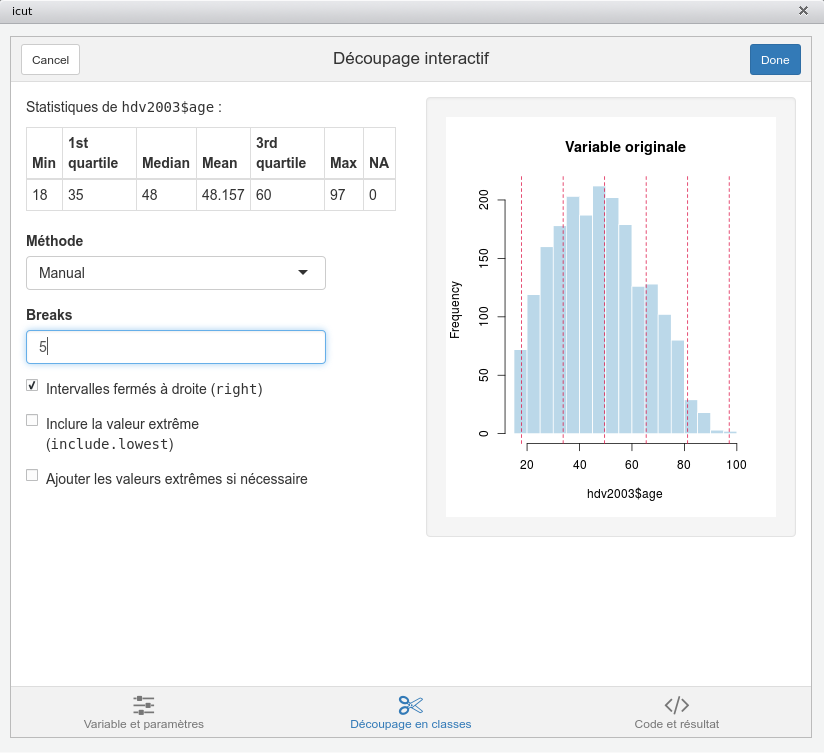
\includegraphics[keepaspectratio]{manipulation/ressources/icut.png}}
Une démonstration en vidéo de cet \emph{add-in} est disponible dans le
webin-R \#05 (\emph{recoder des variables}) sur
{[}YouTube{]}(https://youtu.be/CokvTbtWdwc?t=2795).

\url{https://youtu.be/CokvTbtWdwc}

\end{tcolorbox}

\chapter{Combiner plusieurs variables}\label{sec-combiner-variables}

Parfois, on a besoin de créer une nouvelle variable en partant des
valeurs d'une ou plusieurs autres variables. Dans ce cas on peut
utiliser les fonctions \texttt{dplyr::if\_else()} pour les cas les plus
simples, ou \texttt{dplyr::case\_when()} pour les cas plus complexes.

Une fois encore, nous utiliser le jeu de données \texttt{hdv2003} pour
illustrer ces différentes fonctions.

\begin{Shaded}
\begin{Highlighting}[]
\FunctionTok{library}\NormalTok{(tidyverse)}
\FunctionTok{data}\NormalTok{(}\StringTok{"hdv2003"}\NormalTok{, }\AttributeTok{package =} \StringTok{"questionr"}\NormalTok{)}
\end{Highlighting}
\end{Shaded}

\section{if\_else()}\label{if_else}

\texttt{dplyr::if\_else()} prend trois arguments~: un test, les valeurs
à renvoyer si le test est vrai, et les valeurs à renvoyer si le test est
faux.

Voici un exemple simple~:

\begin{Shaded}
\begin{Highlighting}[]
\NormalTok{v }\OtherTok{\textless{}{-}} \FunctionTok{c}\NormalTok{(}\DecValTok{12}\NormalTok{, }\DecValTok{14}\NormalTok{, }\DecValTok{8}\NormalTok{, }\DecValTok{16}\NormalTok{)}
\FunctionTok{if\_else}\NormalTok{(v }\SpecialCharTok{\textgreater{}} \DecValTok{10}\NormalTok{, }\StringTok{"Supérieur à 10"}\NormalTok{, }\StringTok{"Inférieur à 10"}\NormalTok{)}
\end{Highlighting}
\end{Shaded}

\begin{verbatim}
[1] "Supérieur à 10" "Supérieur à 10" "Inférieur à 10" "Supérieur à 10"
\end{verbatim}

La fonction devient plus intéressante avec des tests combinant plusieurs
variables. Par exemple, imaginons qu'on souhaite créer une nouvelle
variable indiquant les hommes de plus de 60 ans~:

\begin{Shaded}
\begin{Highlighting}[]
\NormalTok{hdv2003 }\OtherTok{\textless{}{-}} 
\NormalTok{  hdv2003 }\SpecialCharTok{|\textgreater{}} 
  \FunctionTok{mutate}\NormalTok{(}
    \AttributeTok{statut =} \FunctionTok{if\_else}\NormalTok{(}
\NormalTok{      sexe }\SpecialCharTok{==} \StringTok{"Homme"} \SpecialCharTok{\&}\NormalTok{ age }\SpecialCharTok{\textgreater{}} \DecValTok{60}\NormalTok{,}
      \StringTok{"Homme de plus de 60 ans"}\NormalTok{,}
      \StringTok{"Autre"}
\NormalTok{    )}
\NormalTok{  )}
\NormalTok{hdv2003 }\SpecialCharTok{|\textgreater{}} \FunctionTok{count}\NormalTok{(statut)}
\end{Highlighting}
\end{Shaded}

\begin{verbatim}
                   statut    n
1                   Autre 1778
2 Homme de plus de 60 ans  222
\end{verbatim}

Il est possible d'utiliser des variables ou des combinaisons de
variables au sein du \texttt{dplyr::if\_else()}. Supposons une petite
enquête menée auprès de femmes et d'hommes. Le questionnaire comportait
une question de préférence posée différemment aux femmes et aux hommes
et dont les réponses ont ainsi été collectées dans deux variables
différentes, \emph{pref\_f} et \emph{pref\_h}, que l'on souhaite
combiner en une seule variable. De même, une certaine mesure
quantitative a été réalisée, mais une correction est nécessaire pour
normaliser ce score (retirer 0.4 aux scores des hommes et 0.6 aux scores
des femmes). Cela peut être réalisé avec le code ci-dessous.

\begin{Shaded}
\begin{Highlighting}[]
\NormalTok{df }\OtherTok{\textless{}{-}} \FunctionTok{tibble}\NormalTok{(}
  \AttributeTok{sexe =} \FunctionTok{c}\NormalTok{(}\StringTok{"f"}\NormalTok{, }\StringTok{"f"}\NormalTok{, }\StringTok{"h"}\NormalTok{, }\StringTok{"h"}\NormalTok{),}
  \AttributeTok{pref\_f =} \FunctionTok{c}\NormalTok{(}\StringTok{"a"}\NormalTok{, }\StringTok{"b"}\NormalTok{, }\ConstantTok{NA}\NormalTok{, }\ConstantTok{NA}\NormalTok{),}
  \AttributeTok{pref\_h =} \FunctionTok{c}\NormalTok{(}\ConstantTok{NA}\NormalTok{, }\ConstantTok{NA}\NormalTok{, }\StringTok{"c"}\NormalTok{, }\StringTok{"d"}\NormalTok{),}
  \AttributeTok{mesure =} \FunctionTok{c}\NormalTok{(}\FloatTok{1.2}\NormalTok{, }\FloatTok{4.1}\NormalTok{, }\FloatTok{3.8}\NormalTok{, }\FloatTok{2.7}\NormalTok{)}
\NormalTok{)}
\NormalTok{df}
\end{Highlighting}
\end{Shaded}

\begin{verbatim}
# A tibble: 4 x 4
  sexe  pref_f pref_h mesure
  <chr> <chr>  <chr>   <dbl>
1 f     a      <NA>      1.2
2 f     b      <NA>      4.1
3 h     <NA>   c         3.8
4 h     <NA>   d         2.7
\end{verbatim}

\begin{Shaded}
\begin{Highlighting}[]
\NormalTok{df }\OtherTok{\textless{}{-}} 
\NormalTok{  df }\SpecialCharTok{|\textgreater{}} 
  \FunctionTok{mutate}\NormalTok{(}
    \AttributeTok{pref =} \FunctionTok{if\_else}\NormalTok{(sexe }\SpecialCharTok{==} \StringTok{"f"}\NormalTok{, pref\_f, pref\_h),}
    \AttributeTok{indicateur =} \FunctionTok{if\_else}\NormalTok{(sexe }\SpecialCharTok{==} \StringTok{"h"}\NormalTok{, mesure }\SpecialCharTok{{-}} \FloatTok{0.4}\NormalTok{, mesure }\SpecialCharTok{{-}} \FloatTok{0.6}\NormalTok{)}
\NormalTok{  )}
\NormalTok{df}
\end{Highlighting}
\end{Shaded}

\begin{verbatim}
# A tibble: 4 x 6
  sexe  pref_f pref_h mesure pref  indicateur
  <chr> <chr>  <chr>   <dbl> <chr>      <dbl>
1 f     a      <NA>      1.2 a            0.6
2 f     b      <NA>      4.1 b            3.5
3 h     <NA>   c         3.8 c            3.4
4 h     <NA>   d         2.7 d            2.3
\end{verbatim}

\begin{tcolorbox}[enhanced jigsaw, toptitle=1mm, bottomtitle=1mm, colframe=quarto-callout-important-color-frame, toprule=.15mm, left=2mm, bottomrule=.15mm, opacitybacktitle=0.6, opacityback=0, coltitle=black, breakable, rightrule=.15mm, arc=.35mm, title=\textcolor{quarto-callout-important-color}{\faExclamation}\hspace{0.5em}{if\_else() et ifelse()}, colbacktitle=quarto-callout-important-color!10!white, titlerule=0mm, leftrule=.75mm, colback=white]

La fonction \texttt{dplyr::if\_else()} ressemble à la fonction
\texttt{ifelse()} en base \textbf{R}. Il y a néanmoins quelques petites
différences~:

\begin{itemize}
\tightlist
\item
  \texttt{dplyr::if\_else()} vérifie que les valeurs fournies pour
  \texttt{true} et celles pour false sont du même type et de la même
  classe et renvoie une erreur dans le cas contraire, là où
  \texttt{ifelse()} sera plus permissif~;
\item
  si un vecteur a des attributs (cf.~Chapitre~\ref{sec-attributs}), ils
  seront préservés par \texttt{dplyr::if\_else()} (et pris dans le
  vecteur \texttt{true}), ce que ne fera pas \texttt{if\_else()}~;
\item
  \texttt{dplyr::if\_else()} propose un argument optionnel
  supplémentaire \texttt{missing} pour indiquer les valeurs à retourner
  lorsque le test renvoie \texttt{NA}.
\end{itemize}

\end{tcolorbox}

\section{case\_when()}\label{case_when}

\texttt{dplyr::case\_when()} est une généralisation de
\texttt{dplyr::if\_else()} qui permet d'indiquer plusieurs tests et
leurs valeurs associées.

Imaginons que l'on souhaite créer une nouvelle variable permettant
d'identifier les hommes de plus de 60 ans, les femmes de plus de 60 ans,
et les autres. On peut utiliser la syntaxe suivante~:

\begin{Shaded}
\begin{Highlighting}[]
\NormalTok{hdv2003 }\OtherTok{\textless{}{-}}
\NormalTok{  hdv2003 }\SpecialCharTok{|\textgreater{}} 
  \FunctionTok{mutate}\NormalTok{(}
    \AttributeTok{statut =} \FunctionTok{case\_when}\NormalTok{(}
\NormalTok{      age }\SpecialCharTok{\textgreater{}=} \DecValTok{60} \SpecialCharTok{\&}\NormalTok{ sexe }\SpecialCharTok{==} \StringTok{"Homme"} \SpecialCharTok{\textasciitilde{}} \StringTok{"Homme, 60 et plus"}\NormalTok{,}
\NormalTok{      age }\SpecialCharTok{\textgreater{}=} \DecValTok{60} \SpecialCharTok{\&}\NormalTok{ sexe }\SpecialCharTok{==} \StringTok{"Femme"} \SpecialCharTok{\textasciitilde{}} \StringTok{"Femme, 60 et plus"}\NormalTok{,}
      \ConstantTok{TRUE} \SpecialCharTok{\textasciitilde{}} \StringTok{"Autre"}
\NormalTok{    )}
\NormalTok{  )}
\NormalTok{hdv2003 }\SpecialCharTok{|\textgreater{}} \FunctionTok{count}\NormalTok{(statut)}
\end{Highlighting}
\end{Shaded}

\begin{verbatim}
             statut    n
1             Autre 1484
2 Femme, 60 et plus  278
3 Homme, 60 et plus  238
\end{verbatim}

\texttt{dplyr::case\_when()} prend en arguments une série d'instructions
sous la forme \texttt{condition\ \textasciitilde{}\ valeur}. Il les
exécute une par une, et dès qu'une \texttt{condition} est vraie, il
renvoi la \texttt{valeur} associée.

La clause \texttt{TRUE\ \textasciitilde{}\ "Autre"} permet d'assigner
une valeur à toutes les lignes pour lesquelles aucune des conditions
précédentes n'est vraie.

\begin{tcolorbox}[enhanced jigsaw, toptitle=1mm, bottomtitle=1mm, colframe=quarto-callout-important-color-frame, toprule=.15mm, left=2mm, bottomrule=.15mm, opacitybacktitle=0.6, opacityback=0, coltitle=black, breakable, rightrule=.15mm, arc=.35mm, title=\textcolor{quarto-callout-important-color}{\faExclamation}\hspace{0.5em}{Important}, colbacktitle=quarto-callout-important-color!10!white, titlerule=0mm, leftrule=.75mm, colback=white]

\textbf{Attention~:} comme les conditions sont testées l'une après
l'autre et que la valeur renvoyée est celle correspondant à la première
condition vraie, l'ordre de ces conditions est très important. Il faut
absolument aller du plus spécifique au plus général.

Par exemple le recodage suivant ne fonctionne pas~:

\begin{Shaded}
\begin{Highlighting}[]
\NormalTok{hdv2003 }\OtherTok{\textless{}{-}}
\NormalTok{  hdv2003 }\SpecialCharTok{|\textgreater{}} 
  \FunctionTok{mutate}\NormalTok{(}
    \AttributeTok{statut =} \FunctionTok{case\_when}\NormalTok{(}
\NormalTok{      sexe }\SpecialCharTok{==} \StringTok{"Homme"} \SpecialCharTok{\textasciitilde{}} \StringTok{"Homme"}\NormalTok{,}
\NormalTok{      age }\SpecialCharTok{\textgreater{}=} \DecValTok{60} \SpecialCharTok{\&}\NormalTok{ sexe }\SpecialCharTok{==} \StringTok{"Homme"} \SpecialCharTok{\textasciitilde{}} \StringTok{"Homme, 60 et plus"}\NormalTok{,}
      \ConstantTok{TRUE} \SpecialCharTok{\textasciitilde{}} \StringTok{"Autre"}
\NormalTok{    )}
\NormalTok{  )}
\NormalTok{hdv2003 }\SpecialCharTok{|\textgreater{}} \FunctionTok{count}\NormalTok{(statut)}
\end{Highlighting}
\end{Shaded}

\begin{verbatim}
  statut    n
1  Autre 1101
2  Homme  899
\end{verbatim}

Comme la condition \texttt{sexe\ ==\ "Homme"} est plus générale que
\texttt{sexe\ ==\ "Homme"\ \&\ age\ \textgreater{}\ 60}, cette deuxième
condition n'est jamais testée~! On n'obtiendra jamais la valeur
correspondante.

Pour que ce recodage fonctionne il faut donc changer l'ordre des
conditions pour aller du plus spécifique au plus général~:

\begin{Shaded}
\begin{Highlighting}[]
\NormalTok{hdv2003 }\OtherTok{\textless{}{-}}
\NormalTok{  hdv2003 }\SpecialCharTok{|\textgreater{}} 
  \FunctionTok{mutate}\NormalTok{(}
    \AttributeTok{statut =} \FunctionTok{case\_when}\NormalTok{(}
\NormalTok{      age }\SpecialCharTok{\textgreater{}=} \DecValTok{60} \SpecialCharTok{\&}\NormalTok{ sexe }\SpecialCharTok{==} \StringTok{"Homme"} \SpecialCharTok{\textasciitilde{}} \StringTok{"Homme, 60 et plus"}\NormalTok{,}
\NormalTok{      sexe }\SpecialCharTok{==} \StringTok{"Homme"} \SpecialCharTok{\textasciitilde{}} \StringTok{"Homme"}\NormalTok{,}
      \ConstantTok{TRUE} \SpecialCharTok{\textasciitilde{}} \StringTok{"Autre"}
\NormalTok{    )}
\NormalTok{  )}
\NormalTok{hdv2003 }\SpecialCharTok{|\textgreater{}} \FunctionTok{count}\NormalTok{(statut)}
\end{Highlighting}
\end{Shaded}

\begin{verbatim}
             statut    n
1             Autre 1101
2             Homme  661
3 Homme, 60 et plus  238
\end{verbatim}

C'est pour cela que l'on peut utiliser, en toute dernière condition, la
valeur \texttt{TRUE} pour indiquer dans tous les autres cas.

\end{tcolorbox}

\section{recode\_if()}\label{recode_if}

Parfois, on n'a besoin de ne modifier une variable que pour certaines
observations. Prenons un petit exemple~:

\begin{Shaded}
\begin{Highlighting}[]
\NormalTok{df }\OtherTok{\textless{}{-}} \FunctionTok{tibble}\NormalTok{(}
  \AttributeTok{pref =} \FunctionTok{factor}\NormalTok{(}\FunctionTok{c}\NormalTok{(}\StringTok{"bleu"}\NormalTok{, }\StringTok{"rouge"}\NormalTok{, }\StringTok{"autre"}\NormalTok{, }\StringTok{"rouge"}\NormalTok{, }\StringTok{"autre"}\NormalTok{)),}
  \AttributeTok{autre\_details =} \FunctionTok{c}\NormalTok{(}\ConstantTok{NA}\NormalTok{, }\ConstantTok{NA}\NormalTok{, }\StringTok{"bleu ciel"}\NormalTok{, }\ConstantTok{NA}\NormalTok{, }\StringTok{"jaune"}\NormalTok{)}
\NormalTok{)}
\NormalTok{df}
\end{Highlighting}
\end{Shaded}

\begin{verbatim}
# A tibble: 5 x 2
  pref  autre_details
  <fct> <chr>        
1 bleu  <NA>         
2 rouge <NA>         
3 autre bleu ciel    
4 rouge <NA>         
5 autre jaune        
\end{verbatim}

Nous avons demandé aux enquêtés d'indiquer leur couleur préférée. Ils
pouvaient répondre bleu ou rouge et avait également la possibilité de
choisir autre et d'indiquer la valeur de leur choix dans un champs
textuel libre.

Une des personnes enquêtées a choisi autre et a indiqué dans le champs
texte la valeur bleu ciel. Pour les besoins de l'analyse, on peut
considérer que cette valeur bleu ciel pour être tout simplement recodée
en bleu.

En syntaxe \textbf{R} classique, on pourra simplement faire~:

\begin{Shaded}
\begin{Highlighting}[]
\NormalTok{df}\SpecialCharTok{$}\NormalTok{pref[df}\SpecialCharTok{$}\NormalTok{autre\_details }\SpecialCharTok{==} \StringTok{"bleu ciel"}\NormalTok{] }\OtherTok{\textless{}{-}} \StringTok{"bleu"}
\end{Highlighting}
\end{Shaded}

Avec \texttt{dplyr::if\_else()}, on serait tenté d'écrire~:

\begin{Shaded}
\begin{Highlighting}[]
\NormalTok{df }\SpecialCharTok{|\textgreater{}} 
  \FunctionTok{mutate}\NormalTok{(}\AttributeTok{pref =} \FunctionTok{if\_else}\NormalTok{(autre\_details }\SpecialCharTok{==} \StringTok{"bleu ciel"}\NormalTok{, }\StringTok{"bleu"}\NormalTok{, pref))}
\end{Highlighting}
\end{Shaded}

\begin{verbatim}
# A tibble: 5 x 2
  pref  autre_details
  <chr> <chr>        
1 <NA>  <NA>         
2 <NA>  <NA>         
3 bleu  bleu ciel    
4 <NA>  <NA>         
5 autre jaune        
\end{verbatim}

On obtient une erreur, car \texttt{dplyr::if\_else()} exige les valeurs
fournie pour \texttt{true} et \texttt{false} soient de même type.
Essayons alors~:

\begin{Shaded}
\begin{Highlighting}[]
\NormalTok{df }\SpecialCharTok{|\textgreater{}} 
  \FunctionTok{mutate}\NormalTok{(}\AttributeTok{pref =} \FunctionTok{if\_else}\NormalTok{(autre\_details }\SpecialCharTok{==} \StringTok{"bleu ciel"}\NormalTok{, }\FunctionTok{factor}\NormalTok{(}\StringTok{"bleu"}\NormalTok{), pref))}
\end{Highlighting}
\end{Shaded}

\begin{verbatim}
# A tibble: 5 x 2
  pref  autre_details
  <fct> <chr>        
1 <NA>  <NA>         
2 <NA>  <NA>         
3 bleu  bleu ciel    
4 <NA>  <NA>         
5 autre jaune        
\end{verbatim}

Ici nous avons un autre problème, signalé par un message d'avertissement
(\emph{warning})~: \texttt{dplyr::if\_else()} ne préserve que les
attributs du vecteur passé en \texttt{true} et non ceux passés à
\texttt{false}. Or l'ensemble des modalités (niveaux du facteur) de la
variable \emph{pref} n'ont pas été définis dans \texttt{factor("bleu")}
et sont ainsi perdus, générant une perte de données (valeurs manquantes
\texttt{NA}).

Pour obtenir le bon résultat, il faudrait inverser la condition~:

\begin{Shaded}
\begin{Highlighting}[]
\NormalTok{df }\SpecialCharTok{|\textgreater{}} 
  \FunctionTok{mutate}\NormalTok{(}\AttributeTok{pref =} \FunctionTok{if\_else}\NormalTok{(}
\NormalTok{    autre\_details }\SpecialCharTok{!=} \StringTok{"bleu ciel"}\NormalTok{, }
\NormalTok{    pref, }
    \FunctionTok{factor}\NormalTok{(}\StringTok{"bleu"}\NormalTok{)}
\NormalTok{  ))}
\end{Highlighting}
\end{Shaded}

\begin{verbatim}
# A tibble: 5 x 2
  pref  autre_details
  <fct> <chr>        
1 <NA>  <NA>         
2 <NA>  <NA>         
3 bleu  bleu ciel    
4 <NA>  <NA>         
5 autre jaune        
\end{verbatim}

Mais ce n'est toujours pas suffisant. En effet, la variable
\emph{autre\_details} a des valeurs manquantes pour lesquelles le test
\texttt{autre\_details\ !=\ "bleu\ ciel"} renvoie \texttt{NA} ce qui une
fois encore génère des valeurs manquantes non souhaitées. Dès lors, il
nous faut soit définir l'argument \texttt{missing} de
\texttt{dplyr::if\_else()}, soit être plus précis dans notre test.

\begin{Shaded}
\begin{Highlighting}[]
\NormalTok{df }\SpecialCharTok{|\textgreater{}} 
  \FunctionTok{mutate}\NormalTok{(}\AttributeTok{pref =} \FunctionTok{if\_else}\NormalTok{(}
\NormalTok{    autre\_details }\SpecialCharTok{!=} \StringTok{"bleu ciel"}\NormalTok{, }
\NormalTok{    pref, }
    \FunctionTok{factor}\NormalTok{(}\StringTok{"bleu"}\NormalTok{),}
    \AttributeTok{missing =}\NormalTok{ pref}
\NormalTok{  ))}
\end{Highlighting}
\end{Shaded}

\begin{verbatim}
# A tibble: 5 x 2
  pref  autre_details
  <fct> <chr>        
1 bleu  <NA>         
2 rouge <NA>         
3 bleu  bleu ciel    
4 rouge <NA>         
5 autre jaune        
\end{verbatim}

\begin{Shaded}
\begin{Highlighting}[]
\NormalTok{df }\SpecialCharTok{|\textgreater{}} 
  \FunctionTok{mutate}\NormalTok{(}\AttributeTok{pref =} \FunctionTok{if\_else}\NormalTok{(}
\NormalTok{    autre\_details }\SpecialCharTok{!=} \StringTok{"bleu ciel"} \SpecialCharTok{|} \FunctionTok{is.na}\NormalTok{(autre\_details), }
\NormalTok{    pref, }
    \FunctionTok{factor}\NormalTok{(}\StringTok{"bleu"}\NormalTok{)}
\NormalTok{  ))}
\end{Highlighting}
\end{Shaded}

\begin{verbatim}
# A tibble: 5 x 2
  pref  autre_details
  <fct> <chr>        
1 bleu  <NA>         
2 rouge <NA>         
3 bleu  bleu ciel    
4 rouge <NA>         
5 autre jaune        
\end{verbatim}

Bref, on peut s'en sortir avec \texttt{dplyr::if\_else()} mais ce n'est
pas forcément le plus pratique dans le cas présent. La syntaxe en base
\textbf{R} fonctionne très bien, mais ne peut pas être intégrée à un
enchaînement d'opérations utilisant le \emph{pipe}.

Dans ce genre de situation, on pourra être intéressé par la fonction
\texttt{labelled::recode\_if()} disponible dans le package
\texttt{\{labelled\}}. Elle permet de ne modifier que certaines
observations d'un vecteur en fonction d'une condition. Si la condition
vaut \texttt{FALSE} ou \texttt{NA}, les observations concernées restent
inchangées. Voyons comment cela s'écrit~:

\begin{Shaded}
\begin{Highlighting}[]
\NormalTok{df }\OtherTok{\textless{}{-}}
\NormalTok{  df }\SpecialCharTok{|\textgreater{}} 
  \FunctionTok{mutate}\NormalTok{(}
    \AttributeTok{pref =}\NormalTok{ pref }\SpecialCharTok{|\textgreater{}} 
\NormalTok{      labelled}\SpecialCharTok{::}\FunctionTok{recode\_if}\NormalTok{(autre\_details }\SpecialCharTok{==} \StringTok{"bleu ciel"}\NormalTok{, }\StringTok{"bleu"}\NormalTok{)}
\NormalTok{  )}
\NormalTok{df}
\end{Highlighting}
\end{Shaded}

\begin{verbatim}
# A tibble: 5 x 2
  pref  autre_details
  <fct> <chr>        
1 bleu  <NA>         
2 rouge <NA>         
3 bleu  bleu ciel    
4 rouge <NA>         
5 autre jaune        
\end{verbatim}

C'est tout de suite plus intuitif~!

\chapter{Étiquettes de variables}\label{sec-etiquettes-variables}

\section{Principe}\label{principe}

Les étiquettes de variable permettent de donner un nom long, plus
explicite, aux différentes colonnes d'un tableau de données (ou encore
directement à un vecteur autonome). Dans le champs des grandes enquêtes,
il est fréquent de nommer les variables \emph{q101}, \emph{q102}, etc.
pour refléter le numéro de la question et d'indiquer ce qu'elle
représente (groupe d'âges, milieu de résidence\ldots) avec une
étiquette.

Un usage, introduit par le package \texttt{\{haven\}}, et repris depuis
par de nombreux autres packages dont \texttt{\{gtsummary\}} que nous
aborderons dans de prochains chapitres, consiste à stocker les
étiquettes de variables sous la forme d'un attribut\footnote{Pour plus
  d'information sur les attributs, voir Chapitre~\ref{sec-attributs}.}
\texttt{"label"} attaché au vecteur / à la colonne du tableau.

Le package \texttt{\{labelled\}} permet de manipuler aisément ces
étiquettes de variables.

La visionneuse de données de \textbf{RStudio} sait reconnaître et
afficher ces étiquettes de variable lorsqu'elles existent. Prenons pour
exemple le jeu de données \texttt{gtsummary::trial} dont les colonnes
ont des étiquettes de variable. La commande
\texttt{View(gtsummary::trial)} permet d'ouvrir la visionneuse de
données de \textbf{RStudio}. Comme on peut le constater, une étiquette
de variable est bien présente sous le nom des différentes colonnes.

\begin{figure}

\centering{

\pandocbounded{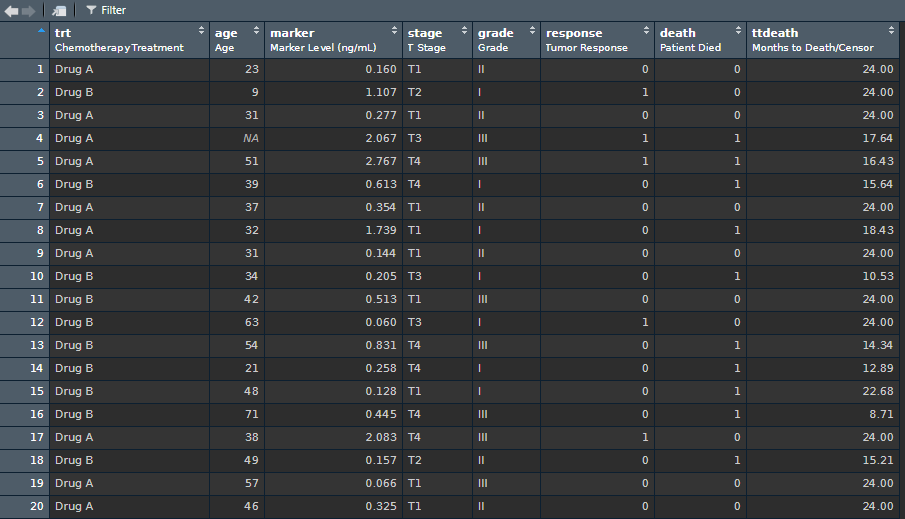
\includegraphics[keepaspectratio]{manipulation/ressources/view_trial.png}}

}

\caption{\label{fig-view-trial}Présentation du tableau
\texttt{gtsummary::trial} dans la visionneuse de \textbf{RStudio}}

\end{figure}%

La fonction \texttt{labelled::look\_for()} du package
\texttt{\{labelled\}} permet de lister l'ensemble des variables d'un
tableau de données et affiche notamment les étiquettes de variable
associées.

\begin{Shaded}
\begin{Highlighting}[]
\FunctionTok{library}\NormalTok{(labelled)}
\NormalTok{gtsummary}\SpecialCharTok{::}\NormalTok{trial }\SpecialCharTok{|\textgreater{}} 
  \FunctionTok{look\_for}\NormalTok{()}
\end{Highlighting}
\end{Shaded}

\begin{verbatim}
 pos variable label                  col_type missing values
 1   trt      Chemotherapy Treatment chr      0             
 2   age      Age                    dbl      11            
 3   marker   Marker Level (ng/mL)   dbl      10            
 4   stage    T Stage                fct      0       T1    
                                                      T2    
                                                      T3    
                                                      T4    
 5   grade    Grade                  fct      0       I     
                                                      II    
                                                      III   
 6   response Tumor Response         int      7             
 7   death    Patient Died           int      0             
 8   ttdeath  Months to Death/Censor dbl      0             
\end{verbatim}

La fonction \texttt{labelled::look\_for()} permet également de
rechercher des variables en tenant compte à la fois de leur nom et de
leur étiquette.

\begin{Shaded}
\begin{Highlighting}[]
\NormalTok{gtsummary}\SpecialCharTok{::}\NormalTok{trial }\SpecialCharTok{|\textgreater{}} 
  \FunctionTok{look\_for}\NormalTok{(}\StringTok{"months"}\NormalTok{)}
\end{Highlighting}
\end{Shaded}

\begin{verbatim}
 pos variable label                  col_type missing values
 8   ttdeath  Months to Death/Censor dbl      0             
\end{verbatim}

\begin{tcolorbox}[enhanced jigsaw, toptitle=1mm, bottomtitle=1mm, colframe=quarto-callout-tip-color-frame, toprule=.15mm, left=2mm, bottomrule=.15mm, opacitybacktitle=0.6, opacityback=0, coltitle=black, breakable, rightrule=.15mm, arc=.35mm, title=\textcolor{quarto-callout-tip-color}{\faLightbulb}\hspace{0.5em}{Astuce}, colbacktitle=quarto-callout-tip-color!10!white, titlerule=0mm, leftrule=.75mm, colback=white]

Comme on le voit, la fonction \texttt{labelled::look\_for()} est tout à
fait adaptée pour générer un dictionnaire de codification. Ses
différentes options sont détaillées dans une
\href{https://larmarange.github.io/labelled/articles/look_for.html}{vignette
dédiée}. Les résultats renvoyés par \texttt{labelled::look\_for()} sont
récupérables dans un tableau de données que l'on pourra ainsi manipuler
à sa guise.

\begin{Shaded}
\begin{Highlighting}[]
\NormalTok{gtsummary}\SpecialCharTok{::}\NormalTok{trial }\SpecialCharTok{|\textgreater{}} 
  \FunctionTok{look\_for}\NormalTok{() }\SpecialCharTok{|\textgreater{}} 
\NormalTok{  dplyr}\SpecialCharTok{::}\FunctionTok{as\_tibble}\NormalTok{()}
\end{Highlighting}
\end{Shaded}

\begin{verbatim}
# A tibble: 8 x 7
    pos variable label                  col_type missing levels     value_labels
  <int> <chr>    <chr>                  <chr>      <int> <named li> <named list>
1     1 trt      Chemotherapy Treatment chr            0 <NULL>     <NULL>      
2     2 age      Age                    dbl           11 <NULL>     <NULL>      
3     3 marker   Marker Level (ng/mL)   dbl           10 <NULL>     <NULL>      
4     4 stage    T Stage                fct            0 <chr [4]>  <NULL>      
5     5 grade    Grade                  fct            0 <chr [3]>  <NULL>      
6     6 response Tumor Response         int            7 <NULL>     <NULL>      
7     7 death    Patient Died           int            0 <NULL>     <NULL>      
8     8 ttdeath  Months to Death/Censor dbl            0 <NULL>     <NULL>      
\end{verbatim}

\end{tcolorbox}

\section{Manipulation sur un vecteur / une
colonne}\label{manipulation-sur-un-vecteur-une-colonne}

La fonction \texttt{labelled::var\_label()} permets de voir l'étiquette
de variable attachée à un vecteur (renvoie \texttt{NULL} s'il n'y en a
pas) mais également d'ajouter/modifier une étiquette.

Le fait d'ajouter une étiquette de variable à un vecteur ne modifie en
rien son type ni sa classe. On peut associer une étiquette de variable à
n'importe quel type de variable, qu'elle soit numérique, textuelle, un
facteur ou encore des dates.

\begin{Shaded}
\begin{Highlighting}[]
\NormalTok{v }\OtherTok{\textless{}{-}} \FunctionTok{c}\NormalTok{(}\DecValTok{1}\NormalTok{, }\DecValTok{5}\NormalTok{, }\DecValTok{2}\NormalTok{, }\DecValTok{4}\NormalTok{, }\DecValTok{1}\NormalTok{)}
\NormalTok{v }\SpecialCharTok{|\textgreater{}} \FunctionTok{var\_label}\NormalTok{()}
\end{Highlighting}
\end{Shaded}

\begin{verbatim}
NULL
\end{verbatim}

\begin{Shaded}
\begin{Highlighting}[]
\FunctionTok{var\_label}\NormalTok{(v) }\OtherTok{\textless{}{-}} \StringTok{"Mon étiquette"}
\FunctionTok{var\_label}\NormalTok{(v)}
\end{Highlighting}
\end{Shaded}

\begin{verbatim}
[1] "Mon étiquette"
\end{verbatim}

\begin{Shaded}
\begin{Highlighting}[]
\FunctionTok{str}\NormalTok{(v)}
\end{Highlighting}
\end{Shaded}

\begin{verbatim}
 num [1:5] 1 5 2 4 1
 - attr(*, "label")= chr "Mon étiquette"
\end{verbatim}

\begin{Shaded}
\begin{Highlighting}[]
\FunctionTok{var\_label}\NormalTok{(v) }\OtherTok{\textless{}{-}} \StringTok{"Une autre étiquette"}
\FunctionTok{var\_label}\NormalTok{(v)}
\end{Highlighting}
\end{Shaded}

\begin{verbatim}
[1] "Une autre étiquette"
\end{verbatim}

\begin{Shaded}
\begin{Highlighting}[]
\FunctionTok{str}\NormalTok{(v)}
\end{Highlighting}
\end{Shaded}

\begin{verbatim}
 num [1:5] 1 5 2 4 1
 - attr(*, "label")= chr "Une autre étiquette"
\end{verbatim}

Pour supprimer une étiquette, il suffit d'attribuer la valeur
\texttt{NULL}.

\begin{Shaded}
\begin{Highlighting}[]
\FunctionTok{var\_label}\NormalTok{(v) }\OtherTok{\textless{}{-}} \ConstantTok{NULL}
\FunctionTok{str}\NormalTok{(v)}
\end{Highlighting}
\end{Shaded}

\begin{verbatim}
 num [1:5] 1 5 2 4 1
\end{verbatim}

On peut appliquer \texttt{labelled::var\_label()} directement sur une
colonne de tableau.

\begin{Shaded}
\begin{Highlighting}[]
\FunctionTok{var\_label}\NormalTok{(iris}\SpecialCharTok{$}\NormalTok{Petal.Length) }\OtherTok{\textless{}{-}} \StringTok{"Longueur du pétale"}
\FunctionTok{var\_label}\NormalTok{(iris}\SpecialCharTok{$}\NormalTok{Petal.Width) }\OtherTok{\textless{}{-}} \StringTok{"Largeur du pétale"}
\FunctionTok{var\_label}\NormalTok{(iris}\SpecialCharTok{$}\NormalTok{Species) }\OtherTok{\textless{}{-}} \StringTok{"Espèce"}
\NormalTok{iris }\SpecialCharTok{|\textgreater{}} 
  \FunctionTok{look\_for}\NormalTok{()}
\end{Highlighting}
\end{Shaded}

\begin{verbatim}
 pos variable     label              col_type missing values    
 1   Sepal.Length —                  dbl      0                 
 2   Sepal.Width  —                  dbl      0                 
 3   Petal.Length Longueur du pétale dbl      0                 
 4   Petal.Width  Largeur du pétale  dbl      0                 
 5   Species      Espèce             fct      0       setosa    
                                                      versicolor
                                                      virginica 
\end{verbatim}

\section{Manipulation sur un tableau de
données}\label{manipulation-sur-un-tableau-de-donnuxe9es}

La fonction \texttt{labelled::set\_variable\_labels()} permets de
manipuler les étiquettes de variable d'un tableau de données avec une
syntaxe du type \texttt{\{dplyr\}}.

\begin{Shaded}
\begin{Highlighting}[]
\NormalTok{iris }\OtherTok{\textless{}{-}} 
\NormalTok{  iris }\SpecialCharTok{|\textgreater{}} 
  \FunctionTok{set\_variable\_labels}\NormalTok{(}
    \AttributeTok{Species =} \ConstantTok{NULL}\NormalTok{,}
    \AttributeTok{Sepal.Length =} \StringTok{"Longeur du sépale"}
\NormalTok{  )}
\NormalTok{iris }\SpecialCharTok{|\textgreater{}} 
  \FunctionTok{look\_for}\NormalTok{()}
\end{Highlighting}
\end{Shaded}

\begin{verbatim}
 pos variable     label              col_type missing values    
 1   Sepal.Length Longeur du sépale  dbl      0                 
 2   Sepal.Width  —                  dbl      0                 
 3   Petal.Length Longueur du pétale dbl      0                 
 4   Petal.Width  Largeur du pétale  dbl      0                 
 5   Species      —                  fct      0       setosa    
                                                      versicolor
                                                      virginica 
\end{verbatim}

\section{Préserver les étiquettes}\label{pruxe9server-les-uxe9tiquettes}

Certaines fonctions de \textbf{R} ne préservent pas les attributs et
risquent donc d'effacer les étiquettes de variables que l'on a définit.
Un exemple est la fonction générique \texttt{subset()} qui permet de
sélectionner certaines lignes remplissant une certaines conditions.

\begin{Shaded}
\begin{Highlighting}[]
\NormalTok{iris }\SpecialCharTok{|\textgreater{}} 
  \FunctionTok{look\_for}\NormalTok{()}
\end{Highlighting}
\end{Shaded}

\begin{verbatim}
 pos variable     label              col_type missing values    
 1   Sepal.Length Longeur du sépale  dbl      0                 
 2   Sepal.Width  —                  dbl      0                 
 3   Petal.Length Longueur du pétale dbl      0                 
 4   Petal.Width  Largeur du pétale  dbl      0                 
 5   Species      —                  fct      0       setosa    
                                                      versicolor
                                                      virginica 
\end{verbatim}

\begin{Shaded}
\begin{Highlighting}[]
\NormalTok{iris }\SpecialCharTok{|\textgreater{}} 
  \FunctionTok{subset}\NormalTok{(Species }\SpecialCharTok{==} \StringTok{"setosa"}\NormalTok{) }\SpecialCharTok{|\textgreater{}} 
  \FunctionTok{look\_for}\NormalTok{()}
\end{Highlighting}
\end{Shaded}

\begin{verbatim}
 pos variable     label col_type missing values    
 1   Sepal.Length —     dbl      0                 
 2   Sepal.Width  —     dbl      0                 
 3   Petal.Length —     dbl      0                 
 4   Petal.Width  —     dbl      0                 
 5   Species      —     fct      0       setosa    
                                         versicolor
                                         virginica 
\end{verbatim}

On pourra, dans ce cas précis, préférer la fonction
\texttt{dplyr::filter()} qui préserve les attributs et donc les
étiquettes de variables.

\begin{Shaded}
\begin{Highlighting}[]
\NormalTok{iris }\SpecialCharTok{|\textgreater{}} 
\NormalTok{  dplyr}\SpecialCharTok{::}\FunctionTok{filter}\NormalTok{(Species }\SpecialCharTok{==} \StringTok{"setosa"}\NormalTok{) }\SpecialCharTok{|\textgreater{}} 
  \FunctionTok{look\_for}\NormalTok{()}
\end{Highlighting}
\end{Shaded}

\begin{verbatim}
 pos variable     label              col_type missing values    
 1   Sepal.Length Longeur du sépale  dbl      0                 
 2   Sepal.Width  —                  dbl      0                 
 3   Petal.Length Longueur du pétale dbl      0                 
 4   Petal.Width  Largeur du pétale  dbl      0                 
 5   Species      —                  fct      0       setosa    
                                                      versicolor
                                                      virginica 
\end{verbatim}

On pourra également tirer parti de la fonction
\texttt{labelled::copy\_labels\_from()} qui permet de copier les
étiquettes d'un tableau à un autre.

\begin{Shaded}
\begin{Highlighting}[]
\NormalTok{iris }\SpecialCharTok{|\textgreater{}} 
  \FunctionTok{subset}\NormalTok{(Species }\SpecialCharTok{==} \StringTok{"setosa"}\NormalTok{) }\SpecialCharTok{|\textgreater{}} 
  \FunctionTok{copy\_labels\_from}\NormalTok{(iris) }\SpecialCharTok{|\textgreater{}} 
  \FunctionTok{look\_for}\NormalTok{()}
\end{Highlighting}
\end{Shaded}

\begin{verbatim}
 pos variable     label              col_type missing values    
 1   Sepal.Length Longeur du sépale  dbl      0                 
 2   Sepal.Width  —                  dbl      0                 
 3   Petal.Length Longueur du pétale dbl      0                 
 4   Petal.Width  Largeur du pétale  dbl      0                 
 5   Species      —                  fct      0       setosa    
                                                      versicolor
                                                      virginica 
\end{verbatim}

\chapter{Étiquettes de valeurs}\label{sec-etiquettes-valeurs}

Dans le domaine des grandes enquêtes, il est fréquent de coder les
variables catégorielles avec des codes numériques auxquels on associé
une certaines valeurs. Par exemple, une variable \emph{milieu de
résidence} pourrait être codée 1 pour urbain, 2 pour semi-urbain, 3 pour
rural et 9 pour indiquer une donnée manquante. Une variable binaire
pourrait quant à elle être codée 0 pour non et 1 pour oui. Souvent,
chaque enquête définit ses propres conventions.

Les logiciels statistiques propriétaires \textbf{SPSS}, \textbf{Stata}
et \textbf{SAS} ont tous les trois un système d'étiquettes de valeurs
pour représenter ce type de variables catégorielles.

\textbf{R} n'a pas, de manière native, de système d'étiquettes de
valeurs. Le format utilisé en interne pour représenter les variables
catégorielles est celui des facteurs (cf.~Chapitre~\ref{sec-facteurs}).
Cependant, ce dernier ne permet de contrôler comment sont associées une
étiquette avec une valeur numérique précise.

\section{\texorpdfstring{La classe
\texttt{haven\_labelled}}{La classe haven\_labelled}}\label{la-classe-haven_labelled}

Afin d'assurer une importation complète des données depuis
\textbf{SPSS}, \textbf{Stata} et \textbf{SAS}, le package
\texttt{\{haven\}} a introduit un nouveau type de vecteurs, la classe
\texttt{haven\_labelled}, qui permet justement de rendre compte de ces
vecteurs labellisés (i.e.~avec des étiquettes de valeurs). Le package
\texttt{\{labelled\}} fournie un jeu de fonctions pour faciliter la
manipulation des vecteurs labellisés.

\begin{tcolorbox}[enhanced jigsaw, toptitle=1mm, bottomtitle=1mm, colframe=quarto-callout-important-color-frame, toprule=.15mm, left=2mm, bottomrule=.15mm, opacitybacktitle=0.6, opacityback=0, coltitle=black, breakable, rightrule=.15mm, arc=.35mm, title=\textcolor{quarto-callout-important-color}{\faExclamation}\hspace{0.5em}{Important}, colbacktitle=quarto-callout-important-color!10!white, titlerule=0mm, leftrule=.75mm, colback=white]

Les vecteurs labellisés sont un format intermédiaire qui permets
d'importer les données telles qu'elles ont été définies dans le fichier
source. Il n'est pas destiné à être utilisé pour l'analyse statistique.

Pour la réalisation de tableaux, graphiques, modèles, \textbf{R} attend
que les variables catégorielles soit codées sous formes de facteurs, et
que les variables continues soient numériques. On aura donc besoin, à un
moment ou à un autre, de convertir les vecteurs labellisés en facteurs
ou en variables numériques classiques.

\end{tcolorbox}

\section{Manipulation sur un vecteur / une
colonne}\label{manipulation-sur-un-vecteur-une-colonne-1}

Pour définir des étiquettes, la fonction de base est
\texttt{labelled::val\_labels()}. Il est possible de définir des
étiquettes de valeurs pour des vecteurs numériques, d'entiers et
textuels. On indiquera les étiquettes sous la forme
\texttt{étiquette\ =\ valeur}. Cette fonction s'utilise de la même
manière que \texttt{labelled::var\_label()} abordée au chapitre
précédent (cf.~Chapitre~\ref{sec-etiquettes-variables}). Un appel simple
renvoie les étiquettes de valeur associées au vecteur, \texttt{NULL}
s'il n'y en n'a pas. Combiner avec l'opérateur d'assignation
(\texttt{\textless{}-}), on peut ajouter/modifier les étiquettes de
valeurs associées au vecteur.

\begin{Shaded}
\begin{Highlighting}[]
\FunctionTok{library}\NormalTok{(labelled)}
\NormalTok{v }\OtherTok{\textless{}{-}} \FunctionTok{c}\NormalTok{(}\DecValTok{1}\NormalTok{, }\DecValTok{2}\NormalTok{, }\DecValTok{1}\NormalTok{, }\DecValTok{9}\NormalTok{)}
\NormalTok{v}
\end{Highlighting}
\end{Shaded}

\begin{verbatim}
[1] 1 2 1 9
\end{verbatim}

\begin{Shaded}
\begin{Highlighting}[]
\FunctionTok{class}\NormalTok{(v)}
\end{Highlighting}
\end{Shaded}

\begin{verbatim}
[1] "numeric"
\end{verbatim}

\begin{Shaded}
\begin{Highlighting}[]
\FunctionTok{val\_labels}\NormalTok{(v)}
\end{Highlighting}
\end{Shaded}

\begin{verbatim}
NULL
\end{verbatim}

\begin{Shaded}
\begin{Highlighting}[]
\FunctionTok{val\_labels}\NormalTok{(v) }\OtherTok{\textless{}{-}} \FunctionTok{c}\NormalTok{(}\AttributeTok{non =} \DecValTok{1}\NormalTok{, }\AttributeTok{oui =} \DecValTok{2}\NormalTok{)}
\FunctionTok{val\_labels}\NormalTok{(v)}
\end{Highlighting}
\end{Shaded}

\begin{verbatim}
non oui 
  1   2 
\end{verbatim}

\begin{Shaded}
\begin{Highlighting}[]
\NormalTok{v}
\end{Highlighting}
\end{Shaded}

\begin{verbatim}
<labelled<double>[4]>
[1] 1 2 1 9

Labels:
 value label
     1   non
     2   oui
\end{verbatim}

\begin{Shaded}
\begin{Highlighting}[]
\FunctionTok{class}\NormalTok{(v)}
\end{Highlighting}
\end{Shaded}

\begin{verbatim}
[1] "haven_labelled" "vctrs_vctr"     "double"        
\end{verbatim}

Comme on peut le voir avec cet exemple simple :

\begin{itemize}
\tightlist
\item
  l'ajout d'étiquettes de valeurs modifie la classe de l'objet (qui est
  maintenant un vecteur de la classe \texttt{haven\_labelled})~;
\item
  l'objet obtenu est multi-classes, la classe \texttt{double} indiquant
  ici qu'il s'agit d'un vecteur numérique~;
\item
  il n'est pas obligatoire d'associer une étiquette de valeurs à toutes
  les valeurs observées dans le vecteur (ici, nous n'avons pas défini
  d'étiquettes pour la valeur \texttt{9}).
\end{itemize}

La fonction \texttt{labelled::val\_label()} (notez l'absence d'un s à la
fin du nom de la fonction) permet d'accéder / de modifier l'étiquette
associée à une valeur spécifique.

\begin{Shaded}
\begin{Highlighting}[]
\FunctionTok{val\_label}\NormalTok{(v, }\DecValTok{1}\NormalTok{)}
\end{Highlighting}
\end{Shaded}

\begin{verbatim}
[1] "non"
\end{verbatim}

\begin{Shaded}
\begin{Highlighting}[]
\FunctionTok{val\_label}\NormalTok{(v, }\DecValTok{9}\NormalTok{)}
\end{Highlighting}
\end{Shaded}

\begin{verbatim}
NULL
\end{verbatim}

\begin{Shaded}
\begin{Highlighting}[]
\FunctionTok{val\_label}\NormalTok{(v, }\DecValTok{9}\NormalTok{) }\OtherTok{\textless{}{-}} \StringTok{"(manquant)"}
\FunctionTok{val\_label}\NormalTok{(v, }\DecValTok{2}\NormalTok{) }\OtherTok{\textless{}{-}} \ConstantTok{NULL}
\NormalTok{v}
\end{Highlighting}
\end{Shaded}

\begin{verbatim}
<labelled<double>[4]>
[1] 1 2 1 9

Labels:
 value      label
     1        non
     9 (manquant)
\end{verbatim}

Pour supprimer, toutes les étiquettes de valeurs, on attribuera
\texttt{NULL} avec \texttt{labelled::val\_labels()}.

\begin{Shaded}
\begin{Highlighting}[]
\FunctionTok{val\_labels}\NormalTok{(v) }\OtherTok{\textless{}{-}} \ConstantTok{NULL}
\NormalTok{v}
\end{Highlighting}
\end{Shaded}

\begin{verbatim}
[1] 1 2 1 9
\end{verbatim}

\begin{Shaded}
\begin{Highlighting}[]
\FunctionTok{class}\NormalTok{(v)}
\end{Highlighting}
\end{Shaded}

\begin{verbatim}
[1] "numeric"
\end{verbatim}

On remarquera que, lorsque toutes les étiquettes de valeurs sont
supprimées, la nature de l'objet change à nouveau et il redevient un
simple vecteur numérique.

\begin{tcolorbox}[enhanced jigsaw, toptitle=1mm, bottomtitle=1mm, colframe=quarto-callout-caution-color-frame, toprule=.15mm, left=2mm, bottomrule=.15mm, opacitybacktitle=0.6, opacityback=0, coltitle=black, breakable, rightrule=.15mm, arc=.35mm, title=\textcolor{quarto-callout-caution-color}{\faFire}\hspace{0.5em}{Mise en garde}, colbacktitle=quarto-callout-caution-color!10!white, titlerule=0mm, leftrule=.75mm, colback=white]

Il est essentiel de bien comprendre que l'ajout d'étiquettes de valeurs
ne change pas fondamentalement la nature du vecteur. \textbf{Cela ne le
transforme pas en variable catégorielle.} À ce stade, le vecteur n'a pas
été transformé en facteur. Cela reste un vecteur numérique qui est
considéré comme tel par \textbf{R}. On peut ainsi en calculer une
moyenne, ce qui serait impossible avec un facteur.

\begin{Shaded}
\begin{Highlighting}[]
\NormalTok{v }\OtherTok{\textless{}{-}} \FunctionTok{c}\NormalTok{(}\DecValTok{1}\NormalTok{, }\DecValTok{2}\NormalTok{, }\DecValTok{1}\NormalTok{, }\DecValTok{2}\NormalTok{)}
\FunctionTok{val\_labels}\NormalTok{(v) }\OtherTok{\textless{}{-}} \FunctionTok{c}\NormalTok{(}\AttributeTok{non =} \DecValTok{1}\NormalTok{, }\AttributeTok{oui =} \DecValTok{2}\NormalTok{)}
\FunctionTok{mean}\NormalTok{(v)}
\end{Highlighting}
\end{Shaded}

\begin{verbatim}
[1] 1.5
\end{verbatim}

\begin{Shaded}
\begin{Highlighting}[]
\NormalTok{f }\OtherTok{\textless{}{-}} \FunctionTok{factor}\NormalTok{(v, }\AttributeTok{levels =} \FunctionTok{c}\NormalTok{(}\DecValTok{1}\NormalTok{, }\DecValTok{2}\NormalTok{), }\AttributeTok{labels =} \FunctionTok{c}\NormalTok{(}\StringTok{"non"}\NormalTok{, }\StringTok{"oui"}\NormalTok{))}
\FunctionTok{mean}\NormalTok{(f)}
\end{Highlighting}
\end{Shaded}

\begin{verbatim}
Warning in mean.default(f): l'argument n'est ni numérique, ni logique : renvoi
de NA
\end{verbatim}

\begin{verbatim}
[1] NA
\end{verbatim}

\end{tcolorbox}

Les fonctions \texttt{labelled::val\_labels()} et
\texttt{labelled::val\_label()} peuvent également être utilisées sur les
colonnes d'un tableau.

\begin{Shaded}
\begin{Highlighting}[]
\NormalTok{df }\OtherTok{\textless{}{-}}\NormalTok{ dplyr}\SpecialCharTok{::}\FunctionTok{tibble}\NormalTok{(}
  \AttributeTok{x =} \FunctionTok{c}\NormalTok{(}\DecValTok{1}\NormalTok{, }\DecValTok{2}\NormalTok{, }\DecValTok{1}\NormalTok{, }\DecValTok{2}\NormalTok{),}
  \AttributeTok{y =} \FunctionTok{c}\NormalTok{(}\DecValTok{3}\NormalTok{, }\DecValTok{9}\NormalTok{, }\DecValTok{9}\NormalTok{, }\DecValTok{3}\NormalTok{)}
\NormalTok{)}
\FunctionTok{val\_labels}\NormalTok{(df}\SpecialCharTok{$}\NormalTok{x) }\OtherTok{\textless{}{-}} \FunctionTok{c}\NormalTok{(}\AttributeTok{non =} \DecValTok{1}\NormalTok{, }\AttributeTok{oui =} \DecValTok{2}\NormalTok{)}
\FunctionTok{val\_label}\NormalTok{(df}\SpecialCharTok{$}\NormalTok{y, }\DecValTok{9}\NormalTok{) }\OtherTok{\textless{}{-}} \StringTok{"(manquant)"}
\NormalTok{df}
\end{Highlighting}
\end{Shaded}

\begin{verbatim}
# A tibble: 4 x 2
  x         y             
  <dbl+lbl> <dbl+lbl>     
1 1 [non]   3             
2 2 [oui]   9 [(manquant)]
3 1 [non]   9 [(manquant)]
4 2 [oui]   3             
\end{verbatim}

On pourra noter, que si notre tableau est un \emph{tibble}, les
étiquettes sont rendues dans la console quand on affiche le tableau.

La fonction \texttt{labelled::look\_for()} est également un bon moyen
d'afficher les étiquettes de valeurs.

\begin{Shaded}
\begin{Highlighting}[]
\NormalTok{df }\SpecialCharTok{|\textgreater{}} 
  \FunctionTok{look\_for}\NormalTok{()}
\end{Highlighting}
\end{Shaded}

\begin{verbatim}
 pos variable label col_type missing values        
 1   x        —     dbl+lbl  0       [1] non       
                                     [2] oui       
 2   y        —     dbl+lbl  0       [9] (manquant)
\end{verbatim}

\section{Manipulation sur un tableau de
données}\label{manipulation-sur-un-tableau-de-donnuxe9es-1}

\texttt{\{labelled\}} fournie 3 fonctions directement applicables sur un
tableau de données~: \texttt{labelled::set\_value\_labels()},
\texttt{labelled::add\_value\_labels()} et
\texttt{labelled::remove\_value\_labels()}. La première remplace
l'ensemble des étiquettes de valeurs associées à une variable, la
seconde ajoute des étiquettes de valeurs (et conserve celles déjà
définies), la troisième supprime les étiquettes associées à certaines
valeurs spécifiques (et laisse les autres inchangées).

\begin{Shaded}
\begin{Highlighting}[]
\NormalTok{df }\SpecialCharTok{|\textgreater{}} 
  \FunctionTok{look\_for}\NormalTok{()}
\end{Highlighting}
\end{Shaded}

\begin{verbatim}
 pos variable label col_type missing values        
 1   x        —     dbl+lbl  0       [1] non       
                                     [2] oui       
 2   y        —     dbl+lbl  0       [9] (manquant)
\end{verbatim}

\begin{Shaded}
\begin{Highlighting}[]
\NormalTok{df }\OtherTok{\textless{}{-}}\NormalTok{ df }\SpecialCharTok{|\textgreater{}} 
  \FunctionTok{set\_value\_labels}\NormalTok{(}
    \AttributeTok{x =} \FunctionTok{c}\NormalTok{(}\AttributeTok{yes =} \DecValTok{2}\NormalTok{),}
    \AttributeTok{y =} \FunctionTok{c}\NormalTok{(}\StringTok{"a répondu"} \OtherTok{=} \DecValTok{3}\NormalTok{, }\StringTok{"refus de répondre"} \OtherTok{=} \DecValTok{9}\NormalTok{)}
\NormalTok{  )}
\NormalTok{df }\SpecialCharTok{|\textgreater{}} 
  \FunctionTok{look\_for}\NormalTok{()}
\end{Highlighting}
\end{Shaded}

\begin{verbatim}
 pos variable label col_type missing values               
 1   x        —     dbl+lbl  0       [2] yes              
 2   y        —     dbl+lbl  0       [3] a répondu        
                                     [9] refus de répondre
\end{verbatim}

\begin{Shaded}
\begin{Highlighting}[]
\NormalTok{df }\OtherTok{\textless{}{-}}\NormalTok{ df }\SpecialCharTok{|\textgreater{}} 
  \FunctionTok{add\_value\_labels}\NormalTok{(}
    \AttributeTok{x =} \FunctionTok{c}\NormalTok{(}\AttributeTok{no =} \DecValTok{1}\NormalTok{)}
\NormalTok{  ) }\SpecialCharTok{|\textgreater{}} 
  \FunctionTok{remove\_value\_labels}\NormalTok{(}
    \AttributeTok{y =} \DecValTok{9}
\NormalTok{  )}
\NormalTok{df }\SpecialCharTok{|\textgreater{}} 
  \FunctionTok{look\_for}\NormalTok{()}
\end{Highlighting}
\end{Shaded}

\begin{verbatim}
 pos variable label col_type missing values       
 1   x        —     dbl+lbl  0       [2] yes      
                                     [1] no       
 2   y        —     dbl+lbl  0       [3] a répondu
\end{verbatim}

\section{Conversion}\label{conversion}

\subsection{Quand convertir les vecteurs labellisés
?}\label{quand-convertir-les-vecteurs-labellisuxe9s}

La classe \texttt{haven\_labelled} permets d'ajouter des métadonnées aux
variables sous la forme d'étiquettes de valeurs. Lorsque les données
sont importées depuis \textbf{SAS}, \textbf{SPSS} ou \textbf{Stata},
cela permet notamment de conserver le codage original du fichier
importé.

Mais il faut noter que ces \emph{étiquettes de valeur} n'indique pas
pour autant de manière systématique le type de variable (catégorielle ou
continue). Les vecteurs labellisés n'ont donc pas vocation à être
utilisés pour l'analyse, notamment le calcul de modèles statistiques.
Ils doivent être convertis en facteurs (pour les variables
catégorielles) ou en vecteurs numériques (pour les variables continues).

La question qui peut se poser est donc de choisir à quel moment cette
conversion doit avoir lieu dans un processus d'analyse. On peut
considérer deux approches principales.

\begin{figure}

\centering{

\pandocbounded{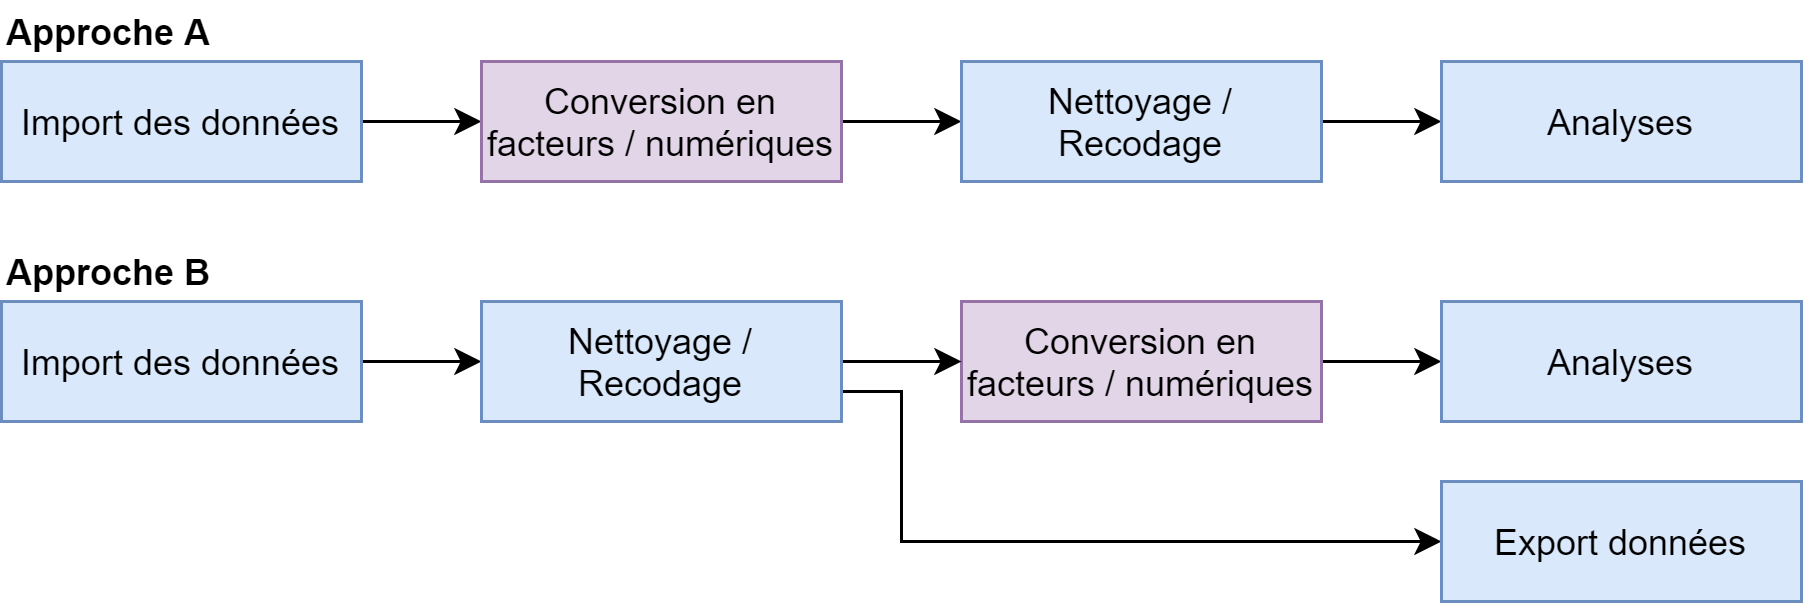
\includegraphics[keepaspectratio]{manipulation/ressources/conversion_labelled.png}}

}

\caption{\label{fig-conversion-labelled}Deux approches possibles pour la
conversion des étiquettes de valeurs}

\end{figure}%

Dans l'\textbf{approche A}, les vecteurs labellisés sont convertis juste
après l'import des données, en utilisant les fonctions
\texttt{labelled::unlabelled()}, \texttt{labelled::to\_factor()} ou
\texttt{base::unclass()} qui sont présentées ci-après. Dès lors, toute
la partie de nettoyage et de recodage des données se fera en utilisant
les fonctions classiques de \textbf{R}. Si l'on n'a pas besoin de
conserver le codage original, cette approche a l'avantage de s'inscrire
dans le fonctionnement usuel de \textbf{R}.

Dans l'\textbf{approche B}, les vecteurs labellisés sont conservés pour
l'étape de nettoyage et de recodage des données. Dans ce cas là, on
pourra avoir recours aux fonctions de l'extension \texttt{\{labelled\}}
qui facilitent la gestion des données labellisées. Cette approche est
particulièrement intéressante quand (i) on veut pouvoir se référer au
dictionnaire de codification fourni avec les données sources et donc on
veut conserver le codage original et/ou (ii) quand les données devront
faire l'objet d'un ré-export après transformation. Par contre, comme
dans l'approche A, il faudra prévoir une conversion des variables
labellisées au moment de l'analyse.

\begin{tcolorbox}[enhanced jigsaw, toptitle=1mm, bottomtitle=1mm, colframe=quarto-callout-warning-color-frame, toprule=.15mm, left=2mm, bottomrule=.15mm, opacitybacktitle=0.6, opacityback=0, coltitle=black, breakable, rightrule=.15mm, arc=.35mm, title=\textcolor{quarto-callout-warning-color}{\faExclamationTriangle}\hspace{0.5em}{Avertissement}, colbacktitle=quarto-callout-warning-color!10!white, titlerule=0mm, leftrule=.75mm, colback=white]

Dans tous les cas, il est recommandé d'adopter l'une ou l'autre
approche, mais d'éviter de mélanger les différents types de vecteur. Une
organisation rigoureuse de ses données et de son code est essentielle~!

\end{tcolorbox}

\subsection{Convertir un vecteur labellisé en
facteur}\label{convertir-un-vecteur-labellisuxe9-en-facteur}

Il est très facile de convertir un vecteur labellisé en facteur à l'aide
la fonction \texttt{labelled::to\_factor()} du package
\texttt{\{labelled\}}\footnote{On privilégiera la fonction
  \texttt{labelled::to\_factor()} à la fonction
  \texttt{haven::as\_factor()} de l'extension \texttt{\{haven\}}, la
  première ayant plus de possibilités et un comportement plus
  consistent.}.

\begin{Shaded}
\begin{Highlighting}[]
\NormalTok{v }\OtherTok{\textless{}{-}} \FunctionTok{c}\NormalTok{(}\DecValTok{1}\NormalTok{,}\DecValTok{2}\NormalTok{,}\DecValTok{9}\NormalTok{,}\DecValTok{3}\NormalTok{,}\DecValTok{3}\NormalTok{,}\DecValTok{2}\NormalTok{,}\ConstantTok{NA}\NormalTok{)}
\FunctionTok{val\_labels}\NormalTok{(v) }\OtherTok{\textless{}{-}} \FunctionTok{c}\NormalTok{(}
  \AttributeTok{oui =} \DecValTok{1}\NormalTok{, }\StringTok{"peut{-}être"} \OtherTok{=} \DecValTok{2}\NormalTok{, }
  \AttributeTok{non =} \DecValTok{3}\NormalTok{, }\StringTok{"ne sait pas"} \OtherTok{=} \DecValTok{9}
\NormalTok{)}
\NormalTok{v}
\end{Highlighting}
\end{Shaded}

\begin{verbatim}
<labelled<double>[7]>
[1]  1  2  9  3  3  2 NA

Labels:
 value       label
     1         oui
     2   peut-être
     3         non
     9 ne sait pas
\end{verbatim}

\begin{Shaded}
\begin{Highlighting}[]
\FunctionTok{to\_factor}\NormalTok{(v)}
\end{Highlighting}
\end{Shaded}

\begin{verbatim}
[1] oui         peut-être   ne sait pas non         non         peut-être  
[7] <NA>       
Levels: oui peut-être non ne sait pas
\end{verbatim}

Il possible d'indiquer si l'on souhaite, comme étiquettes du facteur,
utiliser les étiquettes de valeur (par défaut), les valeurs elles-mêmes,
ou bien les étiquettes de valeurs préfixées par la valeur d'origine
indiquée entre crochets.

\begin{Shaded}
\begin{Highlighting}[]
\FunctionTok{to\_factor}\NormalTok{(v, }\StringTok{\textquotesingle{}l\textquotesingle{}}\NormalTok{)}
\end{Highlighting}
\end{Shaded}

\begin{verbatim}
[1] oui         peut-être   ne sait pas non         non         peut-être  
[7] <NA>       
Levels: oui peut-être non ne sait pas
\end{verbatim}

\begin{Shaded}
\begin{Highlighting}[]
\FunctionTok{to\_factor}\NormalTok{(v, }\StringTok{\textquotesingle{}v\textquotesingle{}}\NormalTok{)}
\end{Highlighting}
\end{Shaded}

\begin{verbatim}
[1] 1    2    9    3    3    2    <NA>
Levels: 1 2 3 9
\end{verbatim}

\begin{Shaded}
\begin{Highlighting}[]
\FunctionTok{to\_factor}\NormalTok{(v, }\StringTok{\textquotesingle{}p\textquotesingle{}}\NormalTok{)}
\end{Highlighting}
\end{Shaded}

\begin{verbatim}
[1] [1] oui         [2] peut-être   [9] ne sait pas [3] non        
[5] [3] non         [2] peut-être   <NA>           
Levels: [1] oui [2] peut-être [3] non [9] ne sait pas
\end{verbatim}

Par défaut, les modalités du facteur seront triées selon l'ordre des
étiquettes de valeur. Mais cela peut être modifié avec l'argument
\texttt{sort\_levels} si l'on préfère trier selon les valeurs ou selon
l'ordre alphabétique des étiquettes.

\begin{Shaded}
\begin{Highlighting}[]
\FunctionTok{to\_factor}\NormalTok{(v, }\AttributeTok{sort\_levels =} \StringTok{\textquotesingle{}v\textquotesingle{}}\NormalTok{)}
\end{Highlighting}
\end{Shaded}

\begin{verbatim}
[1] oui         peut-être   ne sait pas non         non         peut-être  
[7] <NA>       
Levels: oui peut-être non ne sait pas
\end{verbatim}

\begin{Shaded}
\begin{Highlighting}[]
\FunctionTok{to\_factor}\NormalTok{(v, }\AttributeTok{sort\_levels =} \StringTok{\textquotesingle{}l\textquotesingle{}}\NormalTok{)}
\end{Highlighting}
\end{Shaded}

\begin{verbatim}
[1] oui         peut-être   ne sait pas non         non         peut-être  
[7] <NA>       
Levels: ne sait pas non oui peut-être
\end{verbatim}

\subsection{Convertir un vecteur labellisé en numérique ou en
texte}\label{convertir-un-vecteur-labellisuxe9-en-numuxe9rique-ou-en-texte}

Pour rappel, il existe deux types de vecteurs labellisés : des vecteurs
numériques labellisés (\texttt{x} dans l'exemple ci-dessous) et des
vecteurs textuels labellisés (\texttt{y} dans l'exemple ci-dessous).

\begin{Shaded}
\begin{Highlighting}[]
\NormalTok{x }\OtherTok{\textless{}{-}} \FunctionTok{c}\NormalTok{(}\DecValTok{1}\NormalTok{, }\DecValTok{2}\NormalTok{, }\DecValTok{9}\NormalTok{, }\DecValTok{3}\NormalTok{, }\DecValTok{3}\NormalTok{, }\DecValTok{2}\NormalTok{, }\ConstantTok{NA}\NormalTok{)}
\FunctionTok{val\_labels}\NormalTok{(x) }\OtherTok{\textless{}{-}} \FunctionTok{c}\NormalTok{(}
  \AttributeTok{oui =} \DecValTok{1}\NormalTok{, }\StringTok{"peut{-}être"} \OtherTok{=} \DecValTok{2}\NormalTok{, }
  \AttributeTok{non =} \DecValTok{3}\NormalTok{, }\StringTok{"ne sait pas"} \OtherTok{=} \DecValTok{9}
\NormalTok{)}
  
\NormalTok{y }\OtherTok{\textless{}{-}} \FunctionTok{c}\NormalTok{(}\StringTok{"f"}\NormalTok{, }\StringTok{"f"}\NormalTok{, }\StringTok{"h"}\NormalTok{, }\StringTok{"f"}\NormalTok{)}
\FunctionTok{val\_labels}\NormalTok{(y) }\OtherTok{\textless{}{-}} \FunctionTok{c}\NormalTok{(}\AttributeTok{femme =} \StringTok{"f"}\NormalTok{, }\AttributeTok{homme =} \StringTok{"h"}\NormalTok{)}
\end{Highlighting}
\end{Shaded}

Pour leur retirer leur caractère labellisé et revenir à leur classe
d'origine, on peut utiliser la fonction \texttt{unclass()}.

\begin{Shaded}
\begin{Highlighting}[]
\FunctionTok{unclass}\NormalTok{(x)}
\end{Highlighting}
\end{Shaded}

\begin{verbatim}
[1]  1  2  9  3  3  2 NA
attr(,"labels")
        oui   peut-être         non ne sait pas 
          1           2           3           9 
\end{verbatim}

\begin{Shaded}
\begin{Highlighting}[]
\FunctionTok{unclass}\NormalTok{(y)}
\end{Highlighting}
\end{Shaded}

\begin{verbatim}
[1] "f" "f" "h" "f"
attr(,"labels")
femme homme 
  "f"   "h" 
\end{verbatim}

À noter que dans ce cas-là, les étiquettes sont conservées comme
attributs du vecteur.

Une alternative est d'utiliser \texttt{labelled::remove\_labels()} qui
supprimera toutes les étiquettes, y compris les étiquettes de variable.
Pour conserver les étiquettes de variables et ne supprimer que les
étiquettes de valeurs, on indiquera \texttt{keep\_var\_label\ =\ TRUE}.

\begin{Shaded}
\begin{Highlighting}[]
\FunctionTok{var\_label}\NormalTok{(x) }\OtherTok{\textless{}{-}} \StringTok{"Etiquette de variable"}
\FunctionTok{remove\_labels}\NormalTok{(x)}
\end{Highlighting}
\end{Shaded}

\begin{verbatim}
[1]  1  2  9  3  3  2 NA
\end{verbatim}

\begin{Shaded}
\begin{Highlighting}[]
\FunctionTok{remove\_labels}\NormalTok{(x, }\AttributeTok{keep\_var\_label =} \ConstantTok{TRUE}\NormalTok{)}
\end{Highlighting}
\end{Shaded}

\begin{verbatim}
[1]  1  2  9  3  3  2 NA
attr(,"label")
[1] "Etiquette de variable"
\end{verbatim}

\begin{Shaded}
\begin{Highlighting}[]
\FunctionTok{remove\_labels}\NormalTok{(y)}
\end{Highlighting}
\end{Shaded}

\begin{verbatim}
[1] "f" "f" "h" "f"
\end{verbatim}

Dans le cas d'un vecteur numérique labellisé que l'on souhaiterait
convertir en variable textuelle, on pourra utiliser
\texttt{labelled::to\_character()} à la place de
\texttt{labelled::to\_factor()} qui, comme sa grande sœur, utilisera les
étiquettes de valeurs.

\begin{Shaded}
\begin{Highlighting}[]
\FunctionTok{to\_character}\NormalTok{(x)}
\end{Highlighting}
\end{Shaded}

\begin{verbatim}
[1] "oui"         "peut-être"   "ne sait pas" "non"         "non"        
[6] "peut-être"   NA           
attr(,"label")
[1] "Etiquette de variable"
\end{verbatim}

\subsection{Conversion conditionnelle en
facteurs}\label{conversion-conditionnelle-en-facteurs}

Il n'est pas toujours possible de déterminer la nature d'une variable
(continue ou catégorielle) juste à partir de la présence ou l'absence
d'étiquettes de valeur. En effet, on peut utiliser des étiquettes de
valeur dans le cadre d'une variable continue pour indiquer certaines
valeurs spécifiques.

Une bonne pratique est de vérifier chaque variable inclue dans une
analyse, une à une.

Cependant, une règle qui fonctionne dans 90\% des cas est de convertir
un vecteur labellisé en facteur si et seulement si toutes les valeurs
observées dans le vecteur disposent d'une étiquette de valeur
correspondante. C'est ce que propose la fonction
\texttt{labelled::unlabelled()} qui peut même être appliqué à tout un
tableau de données. Par défaut, elle fonctionne ainsi :

\begin{enumerate}
\def\labelenumi{\arabic{enumi}.}
\tightlist
\item
  les variables non labellisées restent inchangées (variables \emph{f}
  et \emph{g} dans l'exemple ci-dessous);
\item
  si toutes les valeurs observées d'une variable labellisées ont une
  étiquette, elles sont converties en facteurs (variables \emph{b} et
  \emph{c});
\item
  sinon, on leur applique \texttt{base::unclass()} (variables \emph{a},
  \emph{d} et \emph{e}).
\end{enumerate}

\begin{Shaded}
\begin{Highlighting}[]
\NormalTok{df }\OtherTok{\textless{}{-}}\NormalTok{ dplyr}\SpecialCharTok{::}\FunctionTok{tibble}\NormalTok{(}
  \AttributeTok{a =} \FunctionTok{c}\NormalTok{(}\DecValTok{1}\NormalTok{, }\DecValTok{1}\NormalTok{, }\DecValTok{2}\NormalTok{, }\DecValTok{3}\NormalTok{),}
  \AttributeTok{b =} \FunctionTok{c}\NormalTok{(}\DecValTok{1}\NormalTok{, }\DecValTok{1}\NormalTok{, }\DecValTok{2}\NormalTok{, }\DecValTok{3}\NormalTok{),}
  \AttributeTok{c =} \FunctionTok{c}\NormalTok{(}\DecValTok{1}\NormalTok{, }\DecValTok{1}\NormalTok{, }\DecValTok{2}\NormalTok{, }\DecValTok{2}\NormalTok{),}
  \AttributeTok{d =} \FunctionTok{c}\NormalTok{(}\StringTok{"a"}\NormalTok{, }\StringTok{"a"}\NormalTok{, }\StringTok{"b"}\NormalTok{, }\StringTok{"c"}\NormalTok{),}
  \AttributeTok{e =} \FunctionTok{c}\NormalTok{(}\DecValTok{1}\NormalTok{, }\DecValTok{9}\NormalTok{, }\DecValTok{1}\NormalTok{, }\DecValTok{2}\NormalTok{),}
  \AttributeTok{f =} \DecValTok{1}\SpecialCharTok{:}\DecValTok{4}\NormalTok{,}
  \AttributeTok{g =} \FunctionTok{as.Date}\NormalTok{(}\FunctionTok{c}\NormalTok{(}
    \StringTok{"2020{-}01{-}01"}\NormalTok{, }\StringTok{"2020{-}02{-}01"}\NormalTok{, }
    \StringTok{"2020{-}03{-}01"}\NormalTok{, }\StringTok{"2020{-}04{-}01"}
\NormalTok{  ))}
\NormalTok{) }\SpecialCharTok{|\textgreater{}} 
  \FunctionTok{set\_value\_labels}\NormalTok{(}
    \AttributeTok{a =} \FunctionTok{c}\NormalTok{(}\AttributeTok{No =} \DecValTok{1}\NormalTok{, }\AttributeTok{Yes =} \DecValTok{2}\NormalTok{),}
    \AttributeTok{b =} \FunctionTok{c}\NormalTok{(}\AttributeTok{No =} \DecValTok{1}\NormalTok{, }\AttributeTok{Yes =} \DecValTok{2}\NormalTok{, }\AttributeTok{DK =} \DecValTok{3}\NormalTok{),}
    \AttributeTok{c =} \FunctionTok{c}\NormalTok{(}\AttributeTok{No =} \DecValTok{1}\NormalTok{, }\AttributeTok{Yes =} \DecValTok{2}\NormalTok{, }\AttributeTok{DK =} \DecValTok{3}\NormalTok{),}
    \AttributeTok{d =} \FunctionTok{c}\NormalTok{(}\AttributeTok{No =} \StringTok{"a"}\NormalTok{, }\AttributeTok{Yes =} \StringTok{"b"}\NormalTok{),}
    \AttributeTok{e =} \FunctionTok{c}\NormalTok{(}\AttributeTok{No =} \DecValTok{1}\NormalTok{, }\AttributeTok{Yes =} \DecValTok{2}\NormalTok{)}
\NormalTok{  )}
\NormalTok{df }\SpecialCharTok{|\textgreater{}} \FunctionTok{look\_for}\NormalTok{()}
\end{Highlighting}
\end{Shaded}

\begin{verbatim}
 pos variable label col_type missing values 
 1   a        —     dbl+lbl  0       [1] No 
                                     [2] Yes
 2   b        —     dbl+lbl  0       [1] No 
                                     [2] Yes
                                     [3] DK 
 3   c        —     dbl+lbl  0       [1] No 
                                     [2] Yes
                                     [3] DK 
 4   d        —     chr+lbl  0       [a] No 
                                     [b] Yes
 5   e        —     dbl+lbl  0       [1] No 
                                     [2] Yes
 6   f        —     int      0              
 7   g        —     date     0              
\end{verbatim}

\begin{Shaded}
\begin{Highlighting}[]
\FunctionTok{to\_factor}\NormalTok{(df) }\SpecialCharTok{|\textgreater{}} \FunctionTok{look\_for}\NormalTok{()}
\end{Highlighting}
\end{Shaded}

\begin{verbatim}
 pos variable label col_type missing values
 1   a        —     fct      0       No    
                                     Yes   
                                     3     
 2   b        —     fct      0       No    
                                     Yes   
                                     DK    
 3   c        —     fct      0       No    
                                     Yes   
                                     DK    
 4   d        —     fct      0       No    
                                     Yes   
                                     c     
 5   e        —     fct      0       No    
                                     Yes   
                                     9     
 6   f        —     int      0             
 7   g        —     date     0             
\end{verbatim}

\begin{Shaded}
\begin{Highlighting}[]
\FunctionTok{unlabelled}\NormalTok{(df) }\SpecialCharTok{|\textgreater{}} \FunctionTok{look\_for}\NormalTok{()}
\end{Highlighting}
\end{Shaded}

\begin{verbatim}
 pos variable label col_type missing values
 1   a        —     dbl      0             
 2   b        —     fct      0       No    
                                     Yes   
                                     DK    
 3   c        —     fct      0       No    
                                     Yes   
                                     DK    
 4   d        —     chr      0             
 5   e        —     dbl      0             
 6   f        —     int      0             
 7   g        —     date     0             
\end{verbatim}

On peut indiquer certaines options, par exemple
\texttt{drop\_unused\_labels\ =\ TRUE} pour supprimer des facteurs créés
les niveaux non observées dans les données (voir la variable \emph{c}).

\begin{Shaded}
\begin{Highlighting}[]
\FunctionTok{unlabelled}\NormalTok{(df, }\AttributeTok{drop\_unused\_labels =} \ConstantTok{TRUE}\NormalTok{) }\SpecialCharTok{|\textgreater{}} 
  \FunctionTok{look\_for}\NormalTok{()}
\end{Highlighting}
\end{Shaded}

\begin{verbatim}
 pos variable label col_type missing values
 1   a        —     dbl      0             
 2   b        —     fct      0       No    
                                     Yes   
                                     DK    
 3   c        —     fct      0       No    
                                     Yes   
 4   d        —     chr      0             
 5   e        —     dbl      0             
 6   f        —     int      0             
 7   g        —     date     0             
\end{verbatim}

\begin{Shaded}
\begin{Highlighting}[]
\FunctionTok{unlabelled}\NormalTok{(df, }\AttributeTok{levels =} \StringTok{"prefixed"}\NormalTok{) }\SpecialCharTok{|\textgreater{}} 
  \FunctionTok{look\_for}\NormalTok{()}
\end{Highlighting}
\end{Shaded}

\begin{verbatim}
 pos variable label col_type missing values 
 1   a        —     dbl      0              
 2   b        —     fct      0       [1] No 
                                     [2] Yes
                                     [3] DK 
 3   c        —     fct      0       [1] No 
                                     [2] Yes
                                     [3] DK 
 4   d        —     chr      0              
 5   e        —     dbl      0              
 6   f        —     int      0              
 7   g        —     date     0              
\end{verbatim}

\chapter{Valeurs manquantes}\label{sec-valeurs-manquantes}

Dans \textbf{R} base, les valeurs manquantes sont indiquées par la
valeurs logiques \texttt{NA} que l'on peut utiliser dans tous types de
vecteurs.

Dans certains cas, par exemple dans la fonction
\texttt{dplyr::if\_else()} qui vérifie que les deux options sont du même
type, on peut avoir besoin de spécifier une valeur manquante d'un
certains types précis (numérique, entier, textuel\ldots) ce que l'on
peut faire avec les constantes \texttt{NA\_real\_},
\texttt{NA\_integer\_} ou encore \texttt{NA\_character\_}.

De base, il n'existe qu'un seul type de valeurs manquantes dans
\textbf{R}. D'autres logiciels statistiques ont mis en place des
systèmes pour distinguer plusieurs types de valeurs manquantes, ce qui
peut avoir une importance dans le domaine des grandes enquêtes, par
exemple pour distinguer des ne sait pas d'un refus de répondre ou d'un
oubli enquêteur.

Ainsi, \textbf{Stata} et \textbf{SAS} ont un système de valeurs
manquantes étiquetées ou \emph{tagged NAs}, où les valeurs manquantes
peuvent recevoir une étiquette (une lettre entre a et z). De son côté,
\textbf{SPSS} permet d'indiquer, sous la forme de métadonnées, que
certaines valeurs devraient être traitées comme des valeurs manquantes
(par exemple que la valeur 8 correspond à des refus et que la valeur 9
correspond à des ne sait pas). Il s'agit alors de valeurs manquantes
définies par l'utilisateur ou \emph{user NAs.}

Dans tous les cas, il appartient à l'analyste de décider au cas par cas
comment ces valeurs manquantes doivent être traitées. Dans le cadre
d'une variable numérique, il est essentiel d'exclure ces valeurs
manquantes pour le calcul de statistiques telles que la moyenne ou
l'écart-type. Pour des variables catégorielles, les pourcentages peuvent
être calculées sur l'ensemble de l'échantillon (les valeurs manquantes
étant alors traitées comme des modalités à part entière) ou bien
uniquement sur les réponses valides, en fonction du besoin de l'analyse
et de ce que l'on cherche à montrer.

Afin d'éviter toute perte d'informations lors d'un import de données
depuis \textbf{Stata}, \textbf{SAS} et \textbf{SPSS}, le package
\texttt{\{haven\}} propose une implémentation sous \textbf{R} des
\emph{tagged NAs} et des \emph{user NAs}. Le package
\texttt{\{labelled\}} fournit quant à lui différentes fonctions pour les
manipuler aisément.

\begin{Shaded}
\begin{Highlighting}[]
\FunctionTok{library}\NormalTok{(labelled)}
\end{Highlighting}
\end{Shaded}

\section{\texorpdfstring{Valeurs manquantes étiquetées (\emph{tagged
NAs})}{Valeurs manquantes étiquetées (tagged NAs)}}\label{sec-tagged-na}

\subsection{Création et test}\label{cruxe9ation-et-test}

Les \emph{tagged NAs} sont de véritables valeurs manquantes
(\texttt{NA}) au sens de \textbf{R}, auxquelles a été attachées sur
étiquette, une lettre unique minuscule (a-z) ou majuscule (A-Z). On peut
les créer avec \texttt{labelled::tagged\_na()}.

\begin{Shaded}
\begin{Highlighting}[]
\NormalTok{x }\OtherTok{\textless{}{-}} \FunctionTok{c}\NormalTok{(}\DecValTok{1}\SpecialCharTok{:}\DecValTok{3}\NormalTok{, }\FunctionTok{tagged\_na}\NormalTok{(}\StringTok{"a"}\NormalTok{), }\FunctionTok{tagged\_na}\NormalTok{(}\StringTok{"z"}\NormalTok{), }\ConstantTok{NA}\NormalTok{)}
\end{Highlighting}
\end{Shaded}

Pour la plupart des fonctions de \textbf{R}, les \emph{tagged NAs} sont
juste considérées comme des valeurs manquantes régulières
(\emph{regular} \emph{NAs}). Dès lors, par défaut, elles sont justes
affichées à l'écran comme n'importe quelle valeur manquante et la
fonction \texttt{is.na()} renvoie \texttt{TRUE}.

\begin{Shaded}
\begin{Highlighting}[]
\NormalTok{x}
\end{Highlighting}
\end{Shaded}

\begin{verbatim}
[1]  1  2  3 NA NA NA
\end{verbatim}

\begin{Shaded}
\begin{Highlighting}[]
\FunctionTok{is.na}\NormalTok{(x)}
\end{Highlighting}
\end{Shaded}

\begin{verbatim}
[1] FALSE FALSE FALSE  TRUE  TRUE  TRUE
\end{verbatim}

Pour afficher les étiquettes associées à ces valeurs manquantes, il faut
avoir recours à \texttt{labelled::na\_tag()},
\texttt{labelled::print\_tagged\_na()} ou encore
\texttt{labelled::format\_tagged\_na()}.

\begin{Shaded}
\begin{Highlighting}[]
\FunctionTok{na\_tag}\NormalTok{(x)}
\end{Highlighting}
\end{Shaded}

\begin{verbatim}
[1] NA  NA  NA  "a" "z" NA 
\end{verbatim}

\begin{Shaded}
\begin{Highlighting}[]
\FunctionTok{print\_tagged\_na}\NormalTok{(x)}
\end{Highlighting}
\end{Shaded}

\begin{verbatim}
[1]     1     2     3 NA(a) NA(z)    NA
\end{verbatim}

\begin{Shaded}
\begin{Highlighting}[]
\FunctionTok{format\_tagged\_na}\NormalTok{(x)}
\end{Highlighting}
\end{Shaded}

\begin{verbatim}
[1] "    1" "    2" "    3" "NA(a)" "NA(z)" "   NA"
\end{verbatim}

Pour tester si une certaine valeur manquante est une \emph{regular NA}
ou une \emph{tagged NA}, on aura recours à
\texttt{labelled::is\_regular\_na()} et à
\texttt{labelled::is\_tagged\_na()}.

\begin{Shaded}
\begin{Highlighting}[]
\FunctionTok{is.na}\NormalTok{(x)}
\end{Highlighting}
\end{Shaded}

\begin{verbatim}
[1] FALSE FALSE FALSE  TRUE  TRUE  TRUE
\end{verbatim}

\begin{Shaded}
\begin{Highlighting}[]
\FunctionTok{is\_regular\_na}\NormalTok{(x)}
\end{Highlighting}
\end{Shaded}

\begin{verbatim}
[1] FALSE FALSE FALSE FALSE FALSE  TRUE
\end{verbatim}

\begin{Shaded}
\begin{Highlighting}[]
\FunctionTok{is\_tagged\_na}\NormalTok{(x)}
\end{Highlighting}
\end{Shaded}

\begin{verbatim}
[1] FALSE FALSE FALSE  TRUE  TRUE FALSE
\end{verbatim}

Il est possible de tester une étiquette particulière en passant un
deuxième argument à \texttt{labelled::is\_tagged\_na()}.

\begin{Shaded}
\begin{Highlighting}[]
\FunctionTok{is\_tagged\_na}\NormalTok{(x, }\StringTok{"a"}\NormalTok{)}
\end{Highlighting}
\end{Shaded}

\begin{verbatim}
[1] FALSE FALSE FALSE  TRUE FALSE FALSE
\end{verbatim}

\begin{tcolorbox}[enhanced jigsaw, toptitle=1mm, bottomtitle=1mm, colframe=quarto-callout-note-color-frame, toprule=.15mm, left=2mm, bottomrule=.15mm, opacitybacktitle=0.6, opacityback=0, coltitle=black, breakable, rightrule=.15mm, arc=.35mm, title=\textcolor{quarto-callout-note-color}{\faInfo}\hspace{0.5em}{Note}, colbacktitle=quarto-callout-note-color!10!white, titlerule=0mm, leftrule=.75mm, colback=white]

Il n'est possible de définir des \emph{tagged NAs} seulement pour des
vecteurs numériques (\emph{double}). Si l'on ajoute une \emph{tagged NA}
à un vecteur d'entiers, ce vecteur sera converti en vecteur numérique.
Si on l'ajoute à un vecteur textuel, la valeur manquante sera convertie
en \emph{regular NA}.

\begin{Shaded}
\begin{Highlighting}[]
\NormalTok{y }\OtherTok{\textless{}{-}} \FunctionTok{c}\NormalTok{(}\StringTok{"a"}\NormalTok{, }\StringTok{"b"}\NormalTok{, }\FunctionTok{tagged\_na}\NormalTok{(}\StringTok{"z"}\NormalTok{))}
\NormalTok{y}
\end{Highlighting}
\end{Shaded}

\begin{verbatim}
[1] "a" "b" NA 
\end{verbatim}

\begin{Shaded}
\begin{Highlighting}[]
\FunctionTok{is\_tagged\_na}\NormalTok{(y)}
\end{Highlighting}
\end{Shaded}

\begin{verbatim}
[1] FALSE FALSE FALSE
\end{verbatim}

\begin{Shaded}
\begin{Highlighting}[]
\FunctionTok{format\_tagged\_na}\NormalTok{(y)}
\end{Highlighting}
\end{Shaded}

\begin{verbatim}
Error: `x` must be a double vector
\end{verbatim}

\begin{Shaded}
\begin{Highlighting}[]
\NormalTok{z }\OtherTok{\textless{}{-}} \FunctionTok{c}\NormalTok{(}\DecValTok{1}\NormalTok{L, }\DecValTok{2}\NormalTok{L, }\FunctionTok{tagged\_na}\NormalTok{(}\StringTok{"a"}\NormalTok{))}
\FunctionTok{typeof}\NormalTok{(z)}
\end{Highlighting}
\end{Shaded}

\begin{verbatim}
[1] "double"
\end{verbatim}

\begin{Shaded}
\begin{Highlighting}[]
\FunctionTok{format\_tagged\_na}\NormalTok{(z)}
\end{Highlighting}
\end{Shaded}

\begin{verbatim}
[1] "    1" "    2" "NA(a)"
\end{verbatim}

\end{tcolorbox}

\subsection{Valeurs uniques, doublons et
tris}\label{valeurs-uniques-doublons-et-tris}

Par défaut, les fonctions classiques de \textbf{R} \texttt{unique()},
\texttt{duplicated()}, \texttt{ordered()} ou encore \texttt{sort()}
traiteront les \emph{tagged NAs} comme des valeurs manquantes tout ce
qu'il y a de plus classique, et ne feront pas de différences entre des
\emph{tagged NAs} ayant des étiquettes différentes.

Pour traiter des \emph{tagged NAs} ayant des étiquettes différentes
comme des valeurs différentes, on aura recours aux fonctions
\texttt{labelled::unique\_tagged\_na()},
\texttt{labelled::duplicated\_tagged\_na()},
\texttt{labelled::order\_tagged\_na()} ou encore
\texttt{labelled::sort\_tagged\_na()}.

\begin{Shaded}
\begin{Highlighting}[]
\NormalTok{x }\OtherTok{\textless{}{-}} \FunctionTok{c}\NormalTok{(}\DecValTok{1}\NormalTok{, }\DecValTok{2}\NormalTok{, }\FunctionTok{tagged\_na}\NormalTok{(}\StringTok{"a"}\NormalTok{), }\DecValTok{1}\NormalTok{, }\FunctionTok{tagged\_na}\NormalTok{(}\StringTok{"z"}\NormalTok{), }\DecValTok{2}\NormalTok{, }\FunctionTok{tagged\_na}\NormalTok{(}\StringTok{"a"}\NormalTok{), }\ConstantTok{NA}\NormalTok{)}
\NormalTok{x }\SpecialCharTok{|\textgreater{}} 
  \FunctionTok{print\_tagged\_na}\NormalTok{()}
\end{Highlighting}
\end{Shaded}

\begin{verbatim}
[1]     1     2 NA(a)     1 NA(z)     2 NA(a)    NA
\end{verbatim}

\begin{Shaded}
\begin{Highlighting}[]
\NormalTok{x }\SpecialCharTok{|\textgreater{}} 
  \FunctionTok{unique}\NormalTok{() }\SpecialCharTok{|\textgreater{}} 
  \FunctionTok{print\_tagged\_na}\NormalTok{()}
\end{Highlighting}
\end{Shaded}

\begin{verbatim}
[1]     1     2 NA(a)
\end{verbatim}

\begin{Shaded}
\begin{Highlighting}[]
\NormalTok{x }\SpecialCharTok{|\textgreater{}} 
  \FunctionTok{unique\_tagged\_na}\NormalTok{() }\SpecialCharTok{|\textgreater{}} 
  \FunctionTok{print\_tagged\_na}\NormalTok{()}
\end{Highlighting}
\end{Shaded}

\begin{verbatim}
[1]     1     2 NA(a) NA(z)    NA
\end{verbatim}

\begin{Shaded}
\begin{Highlighting}[]
\NormalTok{x }\SpecialCharTok{|\textgreater{}} 
  \FunctionTok{duplicated}\NormalTok{()}
\end{Highlighting}
\end{Shaded}

\begin{verbatim}
[1] FALSE FALSE FALSE  TRUE  TRUE  TRUE  TRUE  TRUE
\end{verbatim}

\begin{Shaded}
\begin{Highlighting}[]
\NormalTok{x }\SpecialCharTok{|\textgreater{}} 
  \FunctionTok{duplicated\_tagged\_na}\NormalTok{()}
\end{Highlighting}
\end{Shaded}

\begin{verbatim}
[1] FALSE FALSE FALSE  TRUE FALSE  TRUE  TRUE FALSE
\end{verbatim}

\begin{Shaded}
\begin{Highlighting}[]
\NormalTok{x }\SpecialCharTok{|\textgreater{}} 
  \FunctionTok{sort}\NormalTok{(}\AttributeTok{na.last =} \ConstantTok{TRUE}\NormalTok{) }\SpecialCharTok{|\textgreater{}} 
  \FunctionTok{print\_tagged\_na}\NormalTok{()}
\end{Highlighting}
\end{Shaded}

\begin{verbatim}
[1]     1     1     2     2 NA(a) NA(z) NA(a)    NA
\end{verbatim}

\begin{Shaded}
\begin{Highlighting}[]
\NormalTok{x }\SpecialCharTok{|\textgreater{}} 
  \FunctionTok{sort\_tagged\_na}\NormalTok{()  }\SpecialCharTok{|\textgreater{}} 
  \FunctionTok{print\_tagged\_na}\NormalTok{()}
\end{Highlighting}
\end{Shaded}

\begin{verbatim}
[1]     1     1     2     2 NA(a) NA(a) NA(z)    NA
\end{verbatim}

\subsection{Tagged NAs et étiquettes de
valeurs}\label{tagged-nas-et-uxe9tiquettes-de-valeurs}

Il est tout à fait possible d'associer une étiquette de valeurs
(cf.~Chapitre~\ref{sec-etiquettes-valeurs}) à des \emph{tagged NAs}.

\begin{Shaded}
\begin{Highlighting}[]
\NormalTok{x }\OtherTok{\textless{}{-}} \FunctionTok{c}\NormalTok{(}
  \DecValTok{1}\NormalTok{, }\DecValTok{0}\NormalTok{, }
  \DecValTok{1}\NormalTok{, }\FunctionTok{tagged\_na}\NormalTok{(}\StringTok{"r"}\NormalTok{), }
  \DecValTok{0}\NormalTok{, }\FunctionTok{tagged\_na}\NormalTok{(}\StringTok{"d"}\NormalTok{), }
  \FunctionTok{tagged\_na}\NormalTok{(}\StringTok{"z"}\NormalTok{), }\ConstantTok{NA}
\NormalTok{)}
\FunctionTok{val\_labels}\NormalTok{(x) }\OtherTok{\textless{}{-}} \FunctionTok{c}\NormalTok{(}
  \AttributeTok{no =} \DecValTok{0}\NormalTok{, }
  \AttributeTok{yes =} \DecValTok{1}\NormalTok{,}
  \StringTok{"don\textquotesingle{}t know"} \OtherTok{=} \FunctionTok{tagged\_na}\NormalTok{(}\StringTok{"d"}\NormalTok{),}
  \AttributeTok{refusal =} \FunctionTok{tagged\_na}\NormalTok{(}\StringTok{"r"}\NormalTok{)}
\NormalTok{)}
\NormalTok{x}
\end{Highlighting}
\end{Shaded}

\begin{verbatim}
<labelled<double>[8]>
[1]     1     0     1 NA(r)     0 NA(d) NA(z)    NA

Labels:
 value      label
     0         no
     1        yes
 NA(d) don't know
 NA(r)    refusal
\end{verbatim}

Lorsqu'un vecteur labellisé est converti en facteur avec
\texttt{labelled::to\_factor()}, les \emph{tagged NAs} sont, par défaut
convertis en en valeurs manquantes classiques (\emph{regular NAs}). Il
n'est pas possible de définir des \emph{tagged NAs} pour des facteurs.

\begin{Shaded}
\begin{Highlighting}[]
\NormalTok{x }\SpecialCharTok{|\textgreater{}} \FunctionTok{to\_factor}\NormalTok{()}
\end{Highlighting}
\end{Shaded}

\begin{verbatim}
[1] yes  no   yes  <NA> no   <NA> <NA> <NA>
Levels: no yes
\end{verbatim}

L'option \texttt{explicit\_tagged\_na} de
\texttt{labelled::to\_factor()} permets de convertir les \emph{tagged
NAs} en modalités explicites du facteur.

\begin{Shaded}
\begin{Highlighting}[]
\NormalTok{x }\SpecialCharTok{|\textgreater{}} 
  \FunctionTok{to\_factor}\NormalTok{(}\AttributeTok{explicit\_tagged\_na =} \ConstantTok{TRUE}\NormalTok{)}
\end{Highlighting}
\end{Shaded}

\begin{verbatim}
[1] yes        no         yes        refusal    no         don't know NA(z)     
[8] <NA>      
Levels: no yes don't know refusal NA(z)
\end{verbatim}

\begin{Shaded}
\begin{Highlighting}[]
\NormalTok{x }\SpecialCharTok{|\textgreater{}} 
  \FunctionTok{to\_factor}\NormalTok{(}
    \AttributeTok{levels =} \StringTok{"prefixed"}\NormalTok{, }
    \AttributeTok{explicit\_tagged\_na =} \ConstantTok{TRUE}
\NormalTok{  )}
\end{Highlighting}
\end{Shaded}

\begin{verbatim}
[1] [1] yes            [0] no             [1] yes            [NA(r)] refusal   
[5] [0] no             [NA(d)] don't know [NA(z)] NA(z)      <NA>              
Levels: [0] no [1] yes [NA(d)] don't know [NA(r)] refusal [NA(z)] NA(z)
\end{verbatim}

\subsection{Conversion en user NAs}\label{conversion-en-user-nas}

La fonction \texttt{labelled::tagged\_na\_to\_user\_na()} permets de
convertir des \emph{tagged NAs} en \emph{user NAs}.

\begin{Shaded}
\begin{Highlighting}[]
\NormalTok{x }\SpecialCharTok{|\textgreater{}} 
  \FunctionTok{tagged\_na\_to\_user\_na}\NormalTok{()}
\end{Highlighting}
\end{Shaded}

\begin{verbatim}
<labelled_spss<double>[8]>
[1]  1  0  1  3  0  2  4 NA
Missing range:  [2, 4]

Labels:
 value      label
     0         no
     1        yes
     2 don't know
     3    refusal
     4      NA(z)
\end{verbatim}

\begin{Shaded}
\begin{Highlighting}[]
\NormalTok{x }\SpecialCharTok{|\textgreater{}} 
  \FunctionTok{tagged\_na\_to\_user\_na}\NormalTok{(}\AttributeTok{user\_na\_start =} \DecValTok{10}\NormalTok{)}
\end{Highlighting}
\end{Shaded}

\begin{verbatim}
<labelled_spss<double>[8]>
[1]  1  0  1 11  0 10 12 NA
Missing range:  [10, 12]

Labels:
 value      label
     0         no
     1        yes
    10 don't know
    11    refusal
    12      NA(z)
\end{verbatim}

La fonction \texttt{labelled::tagged\_na\_to\_regular\_na()} convertit
les \emph{tagged NAs} en valeurs manquantes classiques (\emph{regular
NAs}).

\begin{Shaded}
\begin{Highlighting}[]
\NormalTok{x }\SpecialCharTok{|\textgreater{}} 
  \FunctionTok{tagged\_na\_to\_regular\_na}\NormalTok{()}
\end{Highlighting}
\end{Shaded}

\begin{verbatim}
<labelled<double>[8]>
[1]  1  0  1 NA  0 NA NA NA

Labels:
 value label
     0    no
     1   yes
\end{verbatim}

\begin{Shaded}
\begin{Highlighting}[]
\NormalTok{x }\SpecialCharTok{|\textgreater{}} 
  \FunctionTok{tagged\_na\_to\_regular\_na}\NormalTok{() }\SpecialCharTok{|\textgreater{}}
  \FunctionTok{is\_tagged\_na}\NormalTok{()}
\end{Highlighting}
\end{Shaded}

\begin{verbatim}
[1] FALSE FALSE FALSE FALSE FALSE FALSE FALSE FALSE
\end{verbatim}

\section{\texorpdfstring{Valeurs manquantes définies par l'utilisateurs
(\emph{user
NAs})}{Valeurs manquantes définies par l'utilisateurs (user NAs)}}\label{sec-user-na}

Le package \texttt{\{haven\}} a introduit la classe
\texttt{haven\_labelled\_spss}, une extension de la classe
\texttt{haven\_labelled} permettant d'indiquer des valeurs à considérer
comme manquantes à la manière de \textbf{SPSS}.

\begin{tcolorbox}[enhanced jigsaw, toptitle=1mm, bottomtitle=1mm, colframe=quarto-callout-important-color-frame, toprule=.15mm, left=2mm, bottomrule=.15mm, opacitybacktitle=0.6, opacityback=0, coltitle=black, breakable, rightrule=.15mm, arc=.35mm, title=\textcolor{quarto-callout-important-color}{\faExclamation}\hspace{0.5em}{Important}, colbacktitle=quarto-callout-important-color!10!white, titlerule=0mm, leftrule=.75mm, colback=white]

Cela revient à associer à un vecteur des attributs
(cf.~Chapitre~\ref{sec-attributs}) additionnels pour indiquer des
valeurs que l'utilisateur pourrait/devrait considérer comme manquante.
Cependant, il ne s'agit que de métadonnées et en interne ces valeurs ne
sont pas stockées sous forme de \texttt{NA} mais restent des valeurs
valides.

Il convient de garder en mémoire que la très grande majorité des
fonctions de \textbf{R} ne prendront pas en compte ces métadonnées et
traiteront donc ces valeurs comme des valeurs valides. C'est donc à
l'utilisateur de convertir, au besoin, ces les valeurs indiquées comme
manquantes en réelles valeurs manquantes (\texttt{NA}).

\end{tcolorbox}

\subsection{Création}\label{cruxe9ation}

Il est possible d'indiquer des valeurs à considérer comme manquantes
(\emph{user NAs}) de deux manières~:

\begin{itemize}
\tightlist
\item
  soit en indiquant une liste de valeurs individuelles avec
  \texttt{labelled::na\_values()} (on peut indiquer \texttt{NULL} pour
  supprimer les déclarations existantes)~;
\item
  soit en indiquant deux valeurs représentant une plage de valeurs à
  considérées comme manquantes avec \texttt{labelled::na\_range()}
  (seront considérées comme manquantes toutes les valeurs supérieures ou
  égale au premier chiffre et inférieures ou égales au second
  chiffre\footnote{On peut utiler \texttt{-Inf} et \texttt{Inf} qui
    représentent respectivement moins l'infini et l'infini.}).
\end{itemize}

\begin{Shaded}
\begin{Highlighting}[]
\NormalTok{v }\OtherTok{\textless{}{-}} \FunctionTok{c}\NormalTok{(}\DecValTok{1}\NormalTok{, }\DecValTok{2}\NormalTok{, }\DecValTok{3}\NormalTok{, }\DecValTok{9}\NormalTok{, }\DecValTok{1}\NormalTok{, }\DecValTok{3}\NormalTok{, }\DecValTok{2}\NormalTok{, }\ConstantTok{NA}\NormalTok{)}
\FunctionTok{val\_labels}\NormalTok{(v) }\OtherTok{\textless{}{-}} \FunctionTok{c}\NormalTok{(}
  \AttributeTok{faible =} \DecValTok{1}\NormalTok{, }
  \AttributeTok{fort =} \DecValTok{3}\NormalTok{, }
  \StringTok{"ne sait pas"} \OtherTok{=} \DecValTok{9}
\NormalTok{)}
\FunctionTok{na\_values}\NormalTok{(v) }\OtherTok{\textless{}{-}} \DecValTok{9}
\NormalTok{v}
\end{Highlighting}
\end{Shaded}

\begin{verbatim}
<labelled_spss<double>[8]>
[1]  1  2  3  9  1  3  2 NA
Missing values: 9

Labels:
 value       label
     1      faible
     3        fort
     9 ne sait pas
\end{verbatim}

\begin{Shaded}
\begin{Highlighting}[]
\FunctionTok{na\_values}\NormalTok{(v) }\OtherTok{\textless{}{-}} \ConstantTok{NULL}
\NormalTok{v}
\end{Highlighting}
\end{Shaded}

\begin{verbatim}
<labelled<double>[8]>
[1]  1  2  3  9  1  3  2 NA

Labels:
 value       label
     1      faible
     3        fort
     9 ne sait pas
\end{verbatim}

\begin{Shaded}
\begin{Highlighting}[]
\FunctionTok{na\_range}\NormalTok{(v) }\OtherTok{\textless{}{-}} \FunctionTok{c}\NormalTok{(}\DecValTok{5}\NormalTok{, }\ConstantTok{Inf}\NormalTok{)}
\NormalTok{v}
\end{Highlighting}
\end{Shaded}

\begin{verbatim}
<labelled_spss<double>[8]>
[1]  1  2  3  9  1  3  2 NA
Missing range:  [5, Inf]

Labels:
 value       label
     1      faible
     3        fort
     9 ne sait pas
\end{verbatim}

On peut noter que les \emph{user NAs} peuvent cohabiter avec des
\emph{regular NAs} ainsi qu'avec des étiquettes de valeurs (\emph{value
labels}, cf. Chapitre~\ref{sec-etiquettes-valeurs}).

Pour manipuler les variables d'un tableau de données, on peut également
avoir recours à \texttt{labelled::set\_na\_values()} et
\texttt{labelled::set\_na\_range()}.

\begin{Shaded}
\begin{Highlighting}[]
\NormalTok{df }\OtherTok{\textless{}{-}} 
\NormalTok{  dplyr}\SpecialCharTok{::}\FunctionTok{tibble}\NormalTok{(}
    \AttributeTok{s1 =} \FunctionTok{c}\NormalTok{(}\StringTok{"M"}\NormalTok{, }\StringTok{"M"}\NormalTok{, }\StringTok{"F"}\NormalTok{, }\StringTok{"F"}\NormalTok{), }
    \AttributeTok{s2 =} \FunctionTok{c}\NormalTok{(}\DecValTok{1}\NormalTok{, }\DecValTok{1}\NormalTok{, }\DecValTok{2}\NormalTok{, }\DecValTok{9}\NormalTok{)}
\NormalTok{  ) }\SpecialCharTok{|\textgreater{}} 
  \FunctionTok{set\_na\_values}\NormalTok{(}\AttributeTok{s2 =} \DecValTok{9}\NormalTok{)}
\NormalTok{df}\SpecialCharTok{$}\NormalTok{s2}
\end{Highlighting}
\end{Shaded}

\begin{verbatim}
<labelled_spss<double>[4]>
[1] 1 1 2 9
Missing values: 9
\end{verbatim}

\begin{Shaded}
\begin{Highlighting}[]
\NormalTok{df }\OtherTok{\textless{}{-}} 
\NormalTok{  df }\SpecialCharTok{|\textgreater{}} 
  \FunctionTok{set\_na\_values}\NormalTok{(}\AttributeTok{s2 =} \ConstantTok{NULL}\NormalTok{)}
\NormalTok{df}\SpecialCharTok{$}\NormalTok{s2}
\end{Highlighting}
\end{Shaded}

\begin{verbatim}
<labelled<double>[4]>
[1] 1 1 2 9
\end{verbatim}

\subsection{Tests}\label{tests}

La fonction \texttt{is.na()} est l'une des rares fonctions de base
\textbf{R} à reconnaître les \emph{user NAs} et donc à renvoyer
\texttt{TRUE} dans ce cas. Pour des tests plus spécifiques, on aura
recours à \texttt{labelled::is\_user\_na()} et
\texttt{labelled::is\_regular\_na()}.

\begin{Shaded}
\begin{Highlighting}[]
\NormalTok{v}
\end{Highlighting}
\end{Shaded}

\begin{verbatim}
<labelled_spss<double>[8]>
[1]  1  2  3  9  1  3  2 NA
Missing range:  [5, Inf]

Labels:
 value       label
     1      faible
     3        fort
     9 ne sait pas
\end{verbatim}

\begin{Shaded}
\begin{Highlighting}[]
\NormalTok{v }\SpecialCharTok{|\textgreater{}} \FunctionTok{is.na}\NormalTok{()}
\end{Highlighting}
\end{Shaded}

\begin{verbatim}
[1] FALSE FALSE FALSE  TRUE FALSE FALSE FALSE  TRUE
\end{verbatim}

\begin{Shaded}
\begin{Highlighting}[]
\NormalTok{v }\SpecialCharTok{|\textgreater{}} \FunctionTok{is\_user\_na}\NormalTok{()}
\end{Highlighting}
\end{Shaded}

\begin{verbatim}
[1] FALSE FALSE FALSE  TRUE FALSE FALSE FALSE FALSE
\end{verbatim}

\begin{Shaded}
\begin{Highlighting}[]
\NormalTok{v }\SpecialCharTok{|\textgreater{}} \FunctionTok{is\_regular\_na}\NormalTok{()}
\end{Highlighting}
\end{Shaded}

\begin{verbatim}
[1] FALSE FALSE FALSE FALSE FALSE FALSE FALSE  TRUE
\end{verbatim}

\subsection{Conversion}\label{conversion-1}

Comme dit précédemment, pour la plupart des fonctions de \textbf{R}, les
\emph{users NAs} sont toujours des valeurs valides.

\begin{Shaded}
\begin{Highlighting}[]
\NormalTok{x }\OtherTok{\textless{}{-}} \FunctionTok{c}\NormalTok{(}\DecValTok{1}\SpecialCharTok{:}\DecValTok{5}\NormalTok{, }\DecValTok{11}\SpecialCharTok{:}\DecValTok{15}\NormalTok{)}
\FunctionTok{na\_range}\NormalTok{(x) }\OtherTok{\textless{}{-}} \FunctionTok{c}\NormalTok{(}\DecValTok{10}\NormalTok{, }\ConstantTok{Inf}\NormalTok{)}
\NormalTok{x}
\end{Highlighting}
\end{Shaded}

\begin{verbatim}
<labelled_spss<integer>[10]>
 [1]  1  2  3  4  5 11 12 13 14 15
Missing range:  [10, Inf]
\end{verbatim}

\begin{Shaded}
\begin{Highlighting}[]
\FunctionTok{mean}\NormalTok{(x)}
\end{Highlighting}
\end{Shaded}

\begin{verbatim}
[1] 8
\end{verbatim}

On aura alors recours à \texttt{labelled::user\_na\_to\_regular\_na()}
pour convertir les \emph{users NAs} en véritables valeurs manquantes
avant de procéder à un calcul statistique.

\begin{Shaded}
\begin{Highlighting}[]
\NormalTok{x }\SpecialCharTok{|\textgreater{}} 
  \FunctionTok{user\_na\_to\_na}\NormalTok{()}
\end{Highlighting}
\end{Shaded}

\begin{verbatim}
<labelled<integer>[10]>
 [1]  1  2  3  4  5 NA NA NA NA NA
\end{verbatim}

\begin{Shaded}
\begin{Highlighting}[]
\NormalTok{x }\SpecialCharTok{|\textgreater{}} 
  \FunctionTok{user\_na\_to\_na}\NormalTok{() }\SpecialCharTok{|\textgreater{}} 
  \FunctionTok{mean}\NormalTok{(}\AttributeTok{na.rm =} \ConstantTok{TRUE}\NormalTok{)}
\end{Highlighting}
\end{Shaded}

\begin{verbatim}
[1] 3
\end{verbatim}

Une alternative consiste à transformer les \emph{user NAs} en
\emph{tagged NAs} avec \texttt{labelled::user\_na\_to\_tagged\_na()}.

\begin{Shaded}
\begin{Highlighting}[]
\NormalTok{x }\SpecialCharTok{|\textgreater{}} 
  \FunctionTok{user\_na\_to\_tagged\_na}\NormalTok{() }\SpecialCharTok{|\textgreater{}} 
  \FunctionTok{print\_tagged\_na}\NormalTok{()}
\end{Highlighting}
\end{Shaded}

\begin{verbatim}
'x' has been converted into a double vector.
\end{verbatim}

\begin{verbatim}
 [1]     1     2     3     4     5 NA(a) NA(b) NA(c) NA(d) NA(e)
\end{verbatim}

\begin{Shaded}
\begin{Highlighting}[]
\NormalTok{x }\SpecialCharTok{|\textgreater{}} 
  \FunctionTok{user\_na\_to\_tagged\_na}\NormalTok{() }\SpecialCharTok{|\textgreater{}} 
  \FunctionTok{mean}\NormalTok{(}\AttributeTok{na.rm =} \ConstantTok{TRUE}\NormalTok{)}
\end{Highlighting}
\end{Shaded}

\begin{verbatim}
'x' has been converted into a double vector.
\end{verbatim}

\begin{verbatim}
[1] 3
\end{verbatim}

Pour supprimer les métadonnées relatives aux \emph{user NAs} sans les
convertir en valeurs manquantes, on aura recours à
\texttt{labelled::remove\_user\_na()}.

\begin{Shaded}
\begin{Highlighting}[]
\NormalTok{x }\SpecialCharTok{|\textgreater{}}
  \FunctionTok{remove\_user\_na}\NormalTok{()}
\end{Highlighting}
\end{Shaded}

\begin{verbatim}
<labelled<integer>[10]>
 [1]  1  2  3  4  5 11 12 13 14 15
\end{verbatim}

\begin{Shaded}
\begin{Highlighting}[]
\NormalTok{x }\SpecialCharTok{|\textgreater{}} 
  \FunctionTok{remove\_user\_na}\NormalTok{() }\SpecialCharTok{|\textgreater{}} 
  \FunctionTok{mean}\NormalTok{()}
\end{Highlighting}
\end{Shaded}

\begin{verbatim}
[1] 8
\end{verbatim}

Enfin, lorsque l'on convertit un vecteur labellisé en facteur avec
\texttt{labelled::to\_factor()}, on pourra utiliser l'argument
\texttt{user\_na\_to\_na} pour indiquer si les \emph{users NAs} doivent
être convertis ou non en valeurs manquantes classiques (\texttt{NA}).

\begin{Shaded}
\begin{Highlighting}[]
\NormalTok{x }\OtherTok{\textless{}{-}} \FunctionTok{c}\NormalTok{(}\DecValTok{1}\NormalTok{, }\DecValTok{2}\NormalTok{, }\DecValTok{9}\NormalTok{, }\DecValTok{2}\NormalTok{)}
\FunctionTok{val\_labels}\NormalTok{(x) }\OtherTok{\textless{}{-}} \FunctionTok{c}\NormalTok{(}\AttributeTok{oui =} \DecValTok{1}\NormalTok{, }\AttributeTok{non =} \DecValTok{2}\NormalTok{, }\AttributeTok{refus =} \DecValTok{9}\NormalTok{)}
\FunctionTok{na\_values}\NormalTok{(x) }\OtherTok{\textless{}{-}} \DecValTok{9}
\NormalTok{x }\SpecialCharTok{|\textgreater{}}
  \FunctionTok{to\_factor}\NormalTok{(}\AttributeTok{user\_na\_to\_na =} \ConstantTok{TRUE}\NormalTok{)}
\end{Highlighting}
\end{Shaded}

\begin{verbatim}
[1] oui  non  <NA> non 
Levels: oui non
\end{verbatim}

\begin{Shaded}
\begin{Highlighting}[]
\NormalTok{x }\SpecialCharTok{|\textgreater{}}
  \FunctionTok{to\_factor}\NormalTok{(}\AttributeTok{user\_na\_to\_na =} \ConstantTok{FALSE}\NormalTok{)}
\end{Highlighting}
\end{Shaded}

\begin{verbatim}
[1] oui   non   refus non  
Levels: oui non refus
\end{verbatim}

\chapter{Import \& Export de données}\label{sec-import-export}

\section{Importer un fichier texte}\label{importer-un-fichier-texte}

Les fichiers texte constituent un des formats les plus largement
supportés par la majorité des logiciels statistiques. Presque tous
permettent d'exporter des données dans un format texte, y compris les
tableurs comme \textbf{Libre Office}, \textbf{Open Office} ou
\textbf{Excel}.

Cependant, il existe une grande variétés de format texte, qui peuvent
prendre différents noms selon les outils, tels que texte tabulé ou
\emph{texte (séparateur~: tabulation)}, \textbf{CSV} (pour
\emph{comma-separated value}, sachant que suivant les logiciels le
séparateur peut être une virgule ou un point-virgule).

\subsection{Structure d'un fichier
texte}\label{structure-dun-fichier-texte}

Dès lors, avant d'importer un fichier texte dans \textbf{R}, il est
indispensable de regarder comment ce dernier est structuré. Il importe
de prendre note des éléments suivants~:

\begin{itemize}
\tightlist
\item
  La première ligne contient-elle le nom des variables~?
\item
  Quel est le caractère séparateur entre les différentes variables
  (encore appelé séparateur de champs)~? Dans le cadre d'un fichier
  \textbf{CSV}, il aurait pu s'agir d'une virgule ou d'un point-virgule.
\item
  Quel est le caractère utilisé pour indiquer les décimales (le
  séparateur décimal)~? Il s'agit en général d'un point (à
  l'anglo-saxonne) ou d'une virgule (à la française).
\item
  Les valeurs textuelles sont-elles encadrées par des guillemets et, si
  oui, s'agit-il de guillemets simple (\texttt{\textquotesingle{}}) ou
  de guillemets doubles (\texttt{"})~?
\item
  Pour les variables textuelles, y a-t-il des valeurs manquantes et si
  oui comment sont-elles indiquées~? Par exemple, le texte \texttt{NA}
  est parfois utilisé.
\end{itemize}

Il ne faut pas hésitez à ouvrir le fichier avec un éditeur de texte pour
le regarder de plus près.

\subsection{Interface graphique avec
RStudio}\label{interface-graphique-avec-rstudio}

\textbf{RStudio} fournit une interface graphique pour faciliter l'import
d'un fichier texte. Pour cela, il suffit d'aller dans le menu \emph{File
\textgreater{} Import Dataset} et de choisir l'option \emph{From
CSV}\footnote{L'option CSV fonctionne pour tous les fichiers de type
  texte, même si votre fichier a une autre extension, \texttt{.txt} par
  exemple}. Cette option est également disponible via l'onglet
\emph{Environment} dans le quadrant haut-droite.

Pour la suite, nous allons utiliser ce
\href{ressources/exemple_texte_tabule.txt}{fichier texte à titre
d'exemple}.

\begin{figure}

\centering{

\pandocbounded{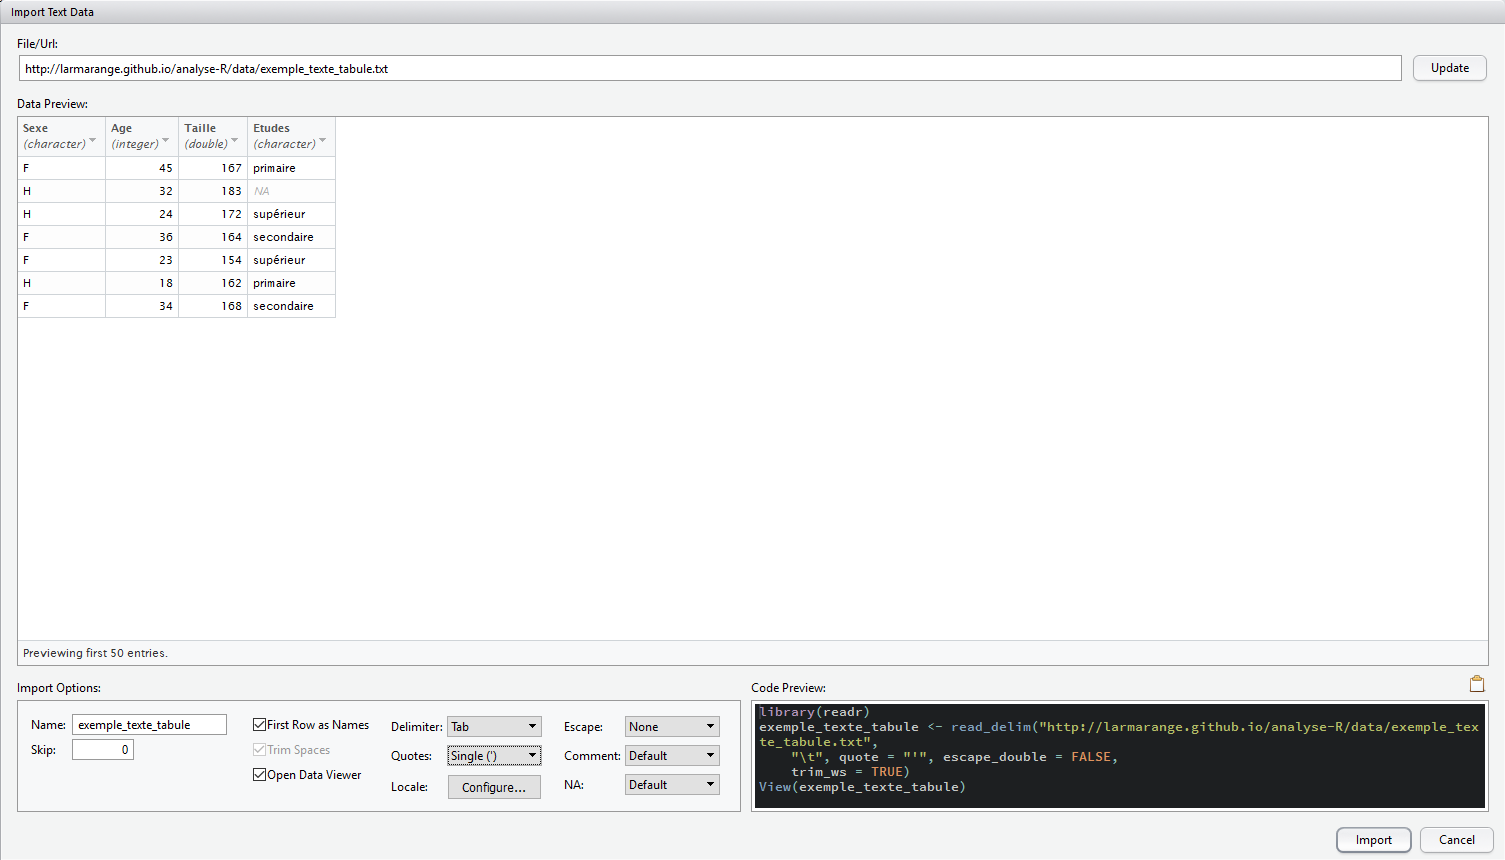
\includegraphics[keepaspectratio]{manipulation/ressources/capture_RStudio_import_readr.png}}

}

\caption{\label{fig-import-rstudio-readr}Importer un fichier texte avec
RStudio}

\end{figure}%

L'interface de \textbf{RStudio} vous présente sous \emph{Import Options}
les différentes options d'import disponible. La section \emph{Data
Preview} vous permet de voir en temps réel comment les données sont
importées. La section \emph{Code Preview} vous indique le code
\textbf{R} correspondant à vos choix. Il n'y a plus qu'à le
copier/coller dans un de vos scripts ou à cliquer sur \textbf{Import}
pour l'exécuter.

Vous pourrez remarquer que \textbf{RStudio} fait appel à l'extension
\texttt{\{readr\}} du tidyverse pour l'import des données via la
fonction \texttt{readr::read\_csv()}.

\texttt{\{readr\}} essaie de deviner le type de chacune des colonnes, en
se basant sur les premières observations. En cliquant sur le nom d'une
colonne, il est possible de modifier le type de la variable importée. Il
est également possible d'exclure une colonne de l'import (\emph{skip}).

\subsection{Dans un script}\label{dans-un-script}

L'interface graphique de \textbf{RStudio} fournit le code d'import. On
peut également l'adapter à ces besoins en consultant la page d'aide de
\texttt{readr::read\_csv()} pour plus de détails. Par exemple~:

\begin{Shaded}
\begin{Highlighting}[]
\FunctionTok{library}\NormalTok{(readr)}
\NormalTok{d }\OtherTok{\textless{}{-}} \FunctionTok{read\_delim}\NormalTok{(}
  \StringTok{"http://larmarange.github.io/analyse{-}R/data/exemple\_texte\_tabule.txt"}\NormalTok{, }
  \AttributeTok{delim =} \StringTok{"}\SpecialCharTok{\textbackslash{}t}\StringTok{"}\NormalTok{, }
  \AttributeTok{quote =} \StringTok{"\textquotesingle{}"}
\NormalTok{)}
\end{Highlighting}
\end{Shaded}

On peut indiquer le chemin local vers un fichier (le plus courant) ou
bien directement l'URL d'un fichier sur Internet.

\texttt{\{readr\}} propose plusieurs fonctions proches~:
\texttt{readr::read\_delim()}, \texttt{readr::read\_csv()},
\texttt{readr::read\_csv2()} et \texttt{readr::read\_tsv()}. Elles
fonctionnent toutes de manière identique et ont les mêmes arguments.
Seule différence, les valeurs par défaut de certains paramètres.

\begin{tcolorbox}[enhanced jigsaw, toptitle=1mm, bottomtitle=1mm, colframe=quarto-callout-tip-color-frame, toprule=.15mm, left=2mm, bottomrule=.15mm, opacitybacktitle=0.6, opacityback=0, coltitle=black, breakable, rightrule=.15mm, arc=.35mm, title=\textcolor{quarto-callout-tip-color}{\faLightbulb}\hspace{0.5em}{Fichiers de très grande taille}, colbacktitle=quarto-callout-tip-color!10!white, titlerule=0mm, leftrule=.75mm, colback=white]

Si vous travaillez sur des données de grandes dimensions, les formats
texte peuvent être lents à exporter et importer. Dans ce cas là, on
pourra jeter un œil au package \texttt{\{vroom\}} et/ou aux fonctions
\texttt{data.table::fread()} et \texttt{data.table::fwrite()}.

\end{tcolorbox}

Dans des manuels ou des exemples en ligne, vous trouverez parfois
mention des fonctions \texttt{utils::read.table()},
\texttt{utils::read.csv()}, \texttt{utils::read.csv2()},
\texttt{utils::read.delim()} ou encore \texttt{utils::read.delim2()}. Il
s'agit des fonctions natives et historiques de \textbf{R} (extension
\texttt{\{utils\}}) dédiées à l'import de fichiers textes. Elles sont
similaires à celles de \texttt{\{readr\}} dans l'idée générale mais
diffèrent dans leurs détails et les traitements effectués sur les
données (pas de détection des dates par exemple). Pour plus
d'information, vous pouvez vous référer à la page d'aide de ces
fonctions.

\section{Importer un fichier Excel}\label{importer-un-fichier-excel}

Une première approche pour importer des données \textbf{Excel} dans
\textbf{R} consiste à les exporter depuis \textbf{Excel} dans un fichier
texte (texte tabulé ou \textbf{CSV}) puis de suivre la procédure
d'importation d'un fichier texte.

Une feuille \textbf{Excel} peut également être importée directement avec
l'extension \texttt{\{readxl\}} du \emph{tidyverse}.

La fonction \texttt{readxl::read\_excel()} permet d'importer à la fois
des fichiers \texttt{.xls} (\textbf{Excel} 2003 et précédents) et
\texttt{.xlsx} (\textbf{Excel} 2007 et suivants).

\begin{Shaded}
\begin{Highlighting}[]
\FunctionTok{library}\NormalTok{(readxl)}
\NormalTok{donnees }\OtherTok{\textless{}{-}} \FunctionTok{read\_excel}\NormalTok{(}\StringTok{"data/fichier.xlsx"}\NormalTok{)}
\end{Highlighting}
\end{Shaded}

Une seule feuille de calculs peut être importée à la fois. On pourra
préciser la feuille désirée avec \texttt{sheet} en indiquant soit le nom
de la feuille, soit sa position (première, seconde, \ldots).

\begin{Shaded}
\begin{Highlighting}[]
\NormalTok{donnees }\OtherTok{\textless{}{-}} \FunctionTok{read\_excel}\NormalTok{(}\StringTok{"data/fichier.xlsx"}\NormalTok{, }\AttributeTok{sheet =} \DecValTok{3}\NormalTok{)}
\NormalTok{donnees }\OtherTok{\textless{}{-}} \FunctionTok{read\_excel}\NormalTok{(}\StringTok{"data/fichier.xlsx"}\NormalTok{, }\AttributeTok{sheet =} \StringTok{"mes\_donnees"}\NormalTok{)}
\end{Highlighting}
\end{Shaded}

On pourra préciser avec \texttt{col\_names} si la première ligne
contient le nom des variables.

Par défaut, \texttt{readxl::read\_excel()} va essayer de deviner le type
(numérique, textuelle, date) de chaque colonne. Au besoin, on pourra
indiquer le type souhaité de chaque colonne avec \texttt{col\_types}.

\textbf{RStudio} propose également pour les fichiers \textbf{Excel} un
assistant d'importation, similaire à celui pour les fichiers texte,
permettant de faciliter l'import.

\section{Importer depuis des logiciels de
statistique}\label{importer-depuis-des-logiciels-de-statistique}

Le package \texttt{\{haven\}} du \emph{tidyverse} a été développé
spécifiquement pour permettre l'importation de données depuis les
formats des logiciels \textbf{Stata}, \textbf{SAS} et \textbf{SPSS}.

Il vise à offrir une importation unifiée depuis ces trois logiciels (là
où le package \texttt{\{foreign\}} distribué en standard avec \textbf{R}
adopte des conventions différentes selon le logiciel source).

Afin de ne pas perdre d'information lors de l'import, \texttt{\{haven\}}
a introduit la notion d'étiquettes de variables
(cf.~Chapitre~\ref{sec-etiquettes-variables}), une classe de vecteurs
pour la gestion des étiquettes de valeurs (cf.
Chapitre~\ref{sec-etiquettes-valeurs}), des mécanismes pour reproduire
la gestion des valeurs manquantes de ces trois logiciels
(cf.~Chapitre~\ref{sec-valeurs-manquantes}), mais également une gestion
et un import correct des dates, dates-heures et des variables horaires
(cf.~le package \texttt{\{hms\}}).

À noter que \textbf{RStudio} intègre également une interface graphique
pour l'import des fichiers \textbf{Stata}, \textbf{SAS} et
\textbf{SPSS}.

\subsection{SPSS}\label{spss}

Les fichiers générés par \textbf{SPSS} sont de deux types~: les fichiers
\textbf{SPSS natifs} (extension \texttt{.sav}) et les fichiers au format
\textbf{SPSS export} (extension \texttt{.por}).

Dans les deux cas, on aura recours à la fonction
\texttt{haven::read\_spss()}~:

\begin{Shaded}
\begin{Highlighting}[]
\FunctionTok{library}\NormalTok{(haven)}
\NormalTok{donnees }\OtherTok{\textless{}{-}} \FunctionTok{read\_spss}\NormalTok{(}\StringTok{"data/fichier.sav"}\NormalTok{, }\AttributeTok{user\_na =} \ConstantTok{TRUE}\NormalTok{)}
\end{Highlighting}
\end{Shaded}

\begin{tcolorbox}[enhanced jigsaw, toptitle=1mm, bottomtitle=1mm, colframe=quarto-callout-tip-color-frame, toprule=.15mm, left=2mm, bottomrule=.15mm, opacitybacktitle=0.6, opacityback=0, coltitle=black, breakable, rightrule=.15mm, arc=.35mm, title=\textcolor{quarto-callout-tip-color}{\faLightbulb}\hspace{0.5em}{Valeurs manquantes}, colbacktitle=quarto-callout-tip-color!10!white, titlerule=0mm, leftrule=.75mm, colback=white]

Dans \textbf{SPSS}, il est possible de définir des valeurs à considérées
comme manquantes ou \emph{user NAs}, voir
Chapitre~\ref{sec-valeurs-manquantes}. Par défaut,
\texttt{haven::read\_spss()} convertir toutes ces valeurs en \texttt{NA}
lors de l'import.

Or, il est parfois important de garder les différentes valeurs
originelles. Dans ce cas, on appellera \texttt{haven::read\_spss()} avec
l'option \texttt{user\_na\ =\ TRUE}.

\end{tcolorbox}

\subsection{SAS}\label{sas}

Les fichiers \textbf{SAS} se présentent en général sous deux format~:
format \textbf{SAS export} (extension \texttt{.xport} ou \texttt{.xpt})
ou format \textbf{SAS natif} (extension \texttt{.sas7bdat}).

Les fichiers \textbf{SAS natifs} peuvent être importées directement avec
\texttt{haven::read\_sas()} de l'extension \texttt{\{haven\}}~:

\begin{Shaded}
\begin{Highlighting}[]
\FunctionTok{library}\NormalTok{(haven)}
\NormalTok{donnees }\OtherTok{\textless{}{-}} \FunctionTok{read\_sas}\NormalTok{(}\StringTok{"data/fichier.sas7bdat"}\NormalTok{)}
\end{Highlighting}
\end{Shaded}

Au besoin, on pourra préciser en deuxième argument le nom d'un fichier
\textbf{SAS catalogue} (extension \texttt{.sas7bcat}) contenant les
métadonnées du fichier de données.

\begin{Shaded}
\begin{Highlighting}[]
\FunctionTok{library}\NormalTok{(haven)}
\NormalTok{donnees }\OtherTok{\textless{}{-}} \FunctionTok{read\_sas}\NormalTok{(}
  \StringTok{"data/fichier.sas7bdat"}\NormalTok{, }
  \AttributeTok{catalog\_file =} \StringTok{"data/fichier.sas7bcat"}
\NormalTok{)}
\end{Highlighting}
\end{Shaded}

\begin{tcolorbox}[enhanced jigsaw, toptitle=1mm, bottomtitle=1mm, colframe=quarto-callout-note-color-frame, toprule=.15mm, left=2mm, bottomrule=.15mm, opacitybacktitle=0.6, opacityback=0, coltitle=black, breakable, rightrule=.15mm, arc=.35mm, title=\textcolor{quarto-callout-note-color}{\faInfo}\hspace{0.5em}{Note}, colbacktitle=quarto-callout-note-color!10!white, titlerule=0mm, leftrule=.75mm, colback=white]

Les fichiers au format \textbf{SAS export} peuvent être importés via la
fonction \texttt{foreign::read.xport()} de l'extension
\texttt{\{foreign\}}. Celle-ci s'utilise très simplement, en lui passant
le nom du fichier en argument~:

\begin{Shaded}
\begin{Highlighting}[]
\FunctionTok{library}\NormalTok{(foreign)}
\NormalTok{donnees }\OtherTok{\textless{}{-}} \FunctionTok{read.xport}\NormalTok{(}\StringTok{"data/fichier.xpt"}\NormalTok{)}
\end{Highlighting}
\end{Shaded}

\end{tcolorbox}

\subsection{Stata}\label{stata}

Pour les fichiers \textbf{Stata} (extension \texttt{.dta}), on aura
recours aux fonctions \texttt{haven::read\_dta()} et
\texttt{haven::read\_stata()} de l'extension \texttt{\{haven\}}. Ces
deux fonctions sont identiques.

\begin{Shaded}
\begin{Highlighting}[]
\FunctionTok{library}\NormalTok{(haven)}
\NormalTok{donnees }\OtherTok{\textless{}{-}} \FunctionTok{read\_dta}\NormalTok{(}\StringTok{"data/fichier.dta"}\NormalTok{)}
\end{Highlighting}
\end{Shaded}

\begin{tcolorbox}[enhanced jigsaw, toptitle=1mm, bottomtitle=1mm, colframe=quarto-callout-important-color-frame, toprule=.15mm, left=2mm, bottomrule=.15mm, opacitybacktitle=0.6, opacityback=0, coltitle=black, breakable, rightrule=.15mm, arc=.35mm, title=\textcolor{quarto-callout-important-color}{\faExclamation}\hspace{0.5em}{Important}, colbacktitle=quarto-callout-important-color!10!white, titlerule=0mm, leftrule=.75mm, colback=white]

\textbf{Gestion des valeurs manquantes}

Dans \textbf{Stata}, il est possible de définir plusieurs types de
valeurs manquantes, qui sont notées sous la forme \texttt{.a} à
\texttt{.z}. Elles sont importées par \texttt{\{haven\}} sous formes de
\emph{tagged NAs}, cf.~Chapitre~\ref{sec-valeurs-manquantes}.

\end{tcolorbox}

\subsection{dBase}\label{dbase}

L'Insee et d'autres producteur de données diffusent leurs fichiers au
format \textbf{dBase} (extension \texttt{.dbf}). Ceux-ci sont
directement lisibles dans \textbf{R} avec la fonction
\texttt{foreign::read.dbf()} de l'extension \texttt{\{foreign\}}.

\begin{Shaded}
\begin{Highlighting}[]
\FunctionTok{library}\NormalTok{(foreign)}
\NormalTok{donnees }\OtherTok{\textless{}{-}} \FunctionTok{read.dbf}\NormalTok{(}\StringTok{"data/fichier.dbf"}\NormalTok{)}
\end{Highlighting}
\end{Shaded}

\section{Sauver ses données}\label{sauver-ses-donnuxe9es}

\textbf{R} dispose également de son propre format pour sauvegarder et
échanger des données. On peut sauver n'importe quel objet créé avec
\textbf{R} et il est possible de sauver plusieurs objets dans un même
fichier. L'usage est d'utiliser l'extension \texttt{.RData} pour les
fichiers de données \textbf{R}. La fonction à utiliser s'appelle tout
simplement \texttt{save()}.

Par exemple, si l'on souhaite sauvegarder son tableau de données
\texttt{d} ainsi que les objets \texttt{tailles} et \texttt{poids} dans
un fichier \texttt{export.RData}~:

\begin{Shaded}
\begin{Highlighting}[]
\FunctionTok{save}\NormalTok{(d, tailles, poids, }\AttributeTok{file =} \StringTok{"export.RData"}\NormalTok{)}
\end{Highlighting}
\end{Shaded}

À tout moment, il sera toujours possible de recharger ces données en
mémoire à l'aide de la fonction \texttt{load()}~:

\begin{Shaded}
\begin{Highlighting}[]
\FunctionTok{load}\NormalTok{(}\StringTok{"export.RData"}\NormalTok{)}
\end{Highlighting}
\end{Shaded}

\begin{tcolorbox}[enhanced jigsaw, toptitle=1mm, bottomtitle=1mm, colframe=quarto-callout-caution-color-frame, toprule=.15mm, left=2mm, bottomrule=.15mm, opacitybacktitle=0.6, opacityback=0, coltitle=black, breakable, rightrule=.15mm, arc=.35mm, title=\textcolor{quarto-callout-caution-color}{\faFire}\hspace{0.5em}{Mise en garde}, colbacktitle=quarto-callout-caution-color!10!white, titlerule=0mm, leftrule=.75mm, colback=white]

Si entre temps vous aviez modifié votre tableau \texttt{d}, vos
modifications seront perdues. En effet, si lors du chargement de
données, un objet du même nom existe en mémoire, ce dernier sera
remplacé par l'objet importé.

\end{tcolorbox}

La fonction \texttt{save.image()} est un raccourci pour sauvegarder tous
les objets de la session de travail dans le fichier \texttt{.RData} (un
fichier un peu étrange car il n'a pas de nom mais juste une extension).
Lors de la fermeture de \textbf{RStudio}, il vous sera demandé si vous
souhaitez enregistrer votre session. Si vous répondez \emph{Oui}, c'est
cette fonction \texttt{save.image()} qui sera appliquée.

\begin{Shaded}
\begin{Highlighting}[]
\FunctionTok{save.image}\NormalTok{()}
\end{Highlighting}
\end{Shaded}

Un autre mécanisme possible est le format \textbf{RDS} de \textbf{R}. La
fonction \texttt{saveRDS()} permet de sauvegarder \textbf{un et un seul}
objet \textbf{R} dans un fichier.

\begin{Shaded}
\begin{Highlighting}[]
\FunctionTok{saveRDS}\NormalTok{(d, }\AttributeTok{file =} \StringTok{"mes\_donnees.rds"}\NormalTok{)}
\end{Highlighting}
\end{Shaded}

Cet objet pourra ensuite être lu avec la fonction \texttt{readRDS()}.
Mais au lieu d'être directement chargé dans la mémoire de
l'environnement de travail, l'objet lu sera retourné par la fonction
\texttt{readRDS()} et ce sera à l'utilisateur de le sauvegarder.

\begin{Shaded}
\begin{Highlighting}[]
\NormalTok{donnees }\OtherTok{\textless{}{-}} \FunctionTok{readRDS}\NormalTok{(}\StringTok{"mes\_donnees.rds"}\NormalTok{)}
\end{Highlighting}
\end{Shaded}

\section{Export de tableaux de
données}\label{export-de-tableaux-de-donnuxe9es}

On peut avoir besoin d'exporter un tableau de données \textbf{R} vers
différents formats. La plupart des fonctions d'import disposent d'un
équivalent permettant l'export de données. On citera notamment~:

\begin{itemize}
\tightlist
\item
  \texttt{readr::write\_csv()} et \texttt{readr::write\_tsv()}
  permettent d'exporter au format \textbf{CSV} et texte tabulé
  respectivement, \texttt{readr::write\_delim()} offrant de multiples
  options pour l\textquotesingle export au format texte~;
\item
  \texttt{haven::write\_sas()} permet d'exporter au format
  \textbf{SAS~;}
\item
  \texttt{haven::write\_sav()} au format \textbf{SPSS~;}
\item
  \texttt{haven::write\_dta()} au format \textbf{Stata~;}
\item
  \texttt{foreign::write.dbf()} au format \textbf{dBase}.
\end{itemize}

L'extension \texttt{readxl} ne fournit pas de fonction pour exporter au
format \textbf{Excel}. Par contre, on pourra passer par la fonction
\texttt{openxlsx::write.xlsx()} du package \texttt{\{openxlsx\}} ou la
fonction \texttt{xlsx::write.xlsx()} de l'extension \texttt{\{xlsx\}}.
L'intérêt de \texttt{\{openxlsx\}} est de ne pas dépendre de
\textbf{Java} à la différence de \texttt{\{xlsx\}}.

\chapter{Mettre en forme des nombres}\label{sec-formater-nombre}

Dans les chapitres suivants, nous aurons régulièrement besoin, pour
produire des tableaux ou des figures propres, de \textbf{fonctions de
formatage} qui permettent de transformer des valeurs numériques en
chaînes de texte.

La fonction \textbf{R} de base est \texttt{format()} mais de nombreux
autres packages proposent des variations pour faciliter cette opération.
Le plus complet est probablement \texttt{\{scales\}} et, notamment, ses
fonctions \texttt{scales::label\_number()} et \texttt{scales::number()}.

Elles ont l'air très similaires et partagent un grand nombre de
paramètres en commun. La différence est que \texttt{scales::number()} a
besoin d'un vecteur numérique en entrée qu'elle va mettre en forme,
tandis que que \texttt{scales::label\_number()} renvoie une fonction que
l'on pourra ensuite appliquer à un vecteur numérique.

\begin{Shaded}
\begin{Highlighting}[]
\FunctionTok{library}\NormalTok{(scales)}
\NormalTok{x }\OtherTok{\textless{}{-}} \FunctionTok{c}\NormalTok{(}\FloatTok{0.0023}\NormalTok{, .}\DecValTok{123}\NormalTok{, }\FloatTok{4.567}\NormalTok{, }\FloatTok{874.44}\NormalTok{, }\DecValTok{8957845}\NormalTok{)}
\FunctionTok{number}\NormalTok{(x)}
\end{Highlighting}
\end{Shaded}

\begin{verbatim}
[1] "0.00"         "0.12"         "4.57"         "874.44"       "8 957 845.00"
\end{verbatim}

\begin{Shaded}
\begin{Highlighting}[]
\NormalTok{f }\OtherTok{\textless{}{-}} \FunctionTok{label\_number}\NormalTok{()}
\FunctionTok{f}\NormalTok{(x)}
\end{Highlighting}
\end{Shaded}

\begin{verbatim}
[1] "0.00"         "0.12"         "4.57"         "874.44"       "8 957 845.00"
\end{verbatim}

\begin{Shaded}
\begin{Highlighting}[]
\FunctionTok{label\_number}\NormalTok{()(x)}
\end{Highlighting}
\end{Shaded}

\begin{verbatim}
[1] "0.00"         "0.12"         "4.57"         "874.44"       "8 957 845.00"
\end{verbatim}

Dans de nombreux cas de figure (par exemple pour un graphique
\texttt{\{ggplot2\}} ou un tableau \texttt{\{gtsummary\}}), il sera
demandé de fournir une fonction de formatage, auquel cas on aura recours
aux fonctions de \texttt{\{scales\}} préfixées par \texttt{label\_*()}
qui permettent donc de générer une fonction personnalisée.

\section{\texorpdfstring{\texttt{label\_number()}}{label\_number()}}\label{label_number}

\texttt{scales::label\_number()} est la fonction de base de mise en
forme de nombres dans \texttt{\{scales\}}, une majorité des autres
fonctions faisant appel à \texttt{scales::label\_number()} et partageant
les mêmes arguments.

Le paramètre \texttt{accurary} permets de définir le niveau d'arrondi à
utiliser. Par exemple, \texttt{.1} pour afficher une seule décimale. Il
est aussi possible d'indiquer un nombre qui n'est pas une puissance de
10 (par exemple \texttt{.25}). Si on n'indique rien (\texttt{NULL}),
alors \texttt{scales::label\_number()} essaiera de deviner un nombre de
décimales pertinent en fonction des valeurs du vecteur de nombres à
mettre en forme.

\begin{Shaded}
\begin{Highlighting}[]
\FunctionTok{label\_number}\NormalTok{(}\AttributeTok{accuracy =} \ConstantTok{NULL}\NormalTok{)(x)}
\end{Highlighting}
\end{Shaded}

\begin{verbatim}
[1] "0.00"         "0.12"         "4.57"         "874.44"       "8 957 845.00"
\end{verbatim}

\begin{Shaded}
\begin{Highlighting}[]
\FunctionTok{label\_number}\NormalTok{(}\AttributeTok{accuracy =}\NormalTok{ .}\DecValTok{1}\NormalTok{)(x)}
\end{Highlighting}
\end{Shaded}

\begin{verbatim}
[1] "0.0"         "0.1"         "4.6"         "874.4"       "8 957 845.0"
\end{verbatim}

\begin{Shaded}
\begin{Highlighting}[]
\FunctionTok{label\_number}\NormalTok{(}\AttributeTok{accuracy =}\NormalTok{ .}\DecValTok{25}\NormalTok{)(x)}
\end{Highlighting}
\end{Shaded}

\begin{verbatim}
[1] "0.0"         "0.0"         "4.5"         "874.5"       "8 957 845.0"
\end{verbatim}

\begin{Shaded}
\begin{Highlighting}[]
\FunctionTok{label\_number}\NormalTok{(}\AttributeTok{accuracy =} \DecValTok{10}\NormalTok{)(x)}
\end{Highlighting}
\end{Shaded}

\begin{verbatim}
[1] "0"         "0"         "0"         "870"       "8 957 840"
\end{verbatim}

L'option \texttt{scale} permets d'indiquer un facteur multiplicatif à
appliquer avant de mettre en forme. On utilisera le plus souvent les
options \texttt{prefix} et \texttt{suffix} en même temps pour indiquer
les unités.

\begin{Shaded}
\begin{Highlighting}[]
\FunctionTok{label\_number}\NormalTok{(}\AttributeTok{scale =} \DecValTok{100}\NormalTok{, }\AttributeTok{suffix =} \StringTok{"\%"}\NormalTok{)(x) }\CommentTok{\# pour cent}
\end{Highlighting}
\end{Shaded}

\begin{verbatim}
[1] "0%"           "12%"          "457%"         "87 444%"      "895 784 500%"
\end{verbatim}

\begin{Shaded}
\begin{Highlighting}[]
\FunctionTok{label\_number}\NormalTok{(}\AttributeTok{scale =} \DecValTok{1000}\NormalTok{, }\AttributeTok{suffix =} \StringTok{"\textbackslash{}u2030"}\NormalTok{)(x) }\CommentTok{\# pour mille}
\end{Highlighting}
\end{Shaded}

\begin{verbatim}
[1] "2‰"             "123‰"           "4 567‰"         "874 440‰"      
[5] "8 957 845 000‰"
\end{verbatim}

\begin{Shaded}
\begin{Highlighting}[]
\FunctionTok{label\_number}\NormalTok{(}\AttributeTok{scale =}\NormalTok{ .}\DecValTok{001}\NormalTok{, }\AttributeTok{suffix =} \StringTok{" milliers"}\NormalTok{, }\AttributeTok{accuracy =}\NormalTok{ .}\DecValTok{1}\NormalTok{)(x)}
\end{Highlighting}
\end{Shaded}

\begin{verbatim}
[1] "0.0 milliers"     "0.0 milliers"     "0.0 milliers"     "0.9 milliers"    
[5] "8 957.8 milliers"
\end{verbatim}

Les arguments \texttt{decimal.mark} et \texttt{big.mark} permettent de
définir, respectivement, le séparateur de décimale et le séparateur de
milliers. Ainsi, pour afficher des nombres à la française (virgule pour
les décimales, espace pour les milliers)~:

\begin{Shaded}
\begin{Highlighting}[]
\FunctionTok{label\_number}\NormalTok{(}\AttributeTok{decimal.mark =} \StringTok{","}\NormalTok{, }\AttributeTok{big.mark =} \StringTok{" "}\NormalTok{)(x)}
\end{Highlighting}
\end{Shaded}

\begin{verbatim}
[1] "0,00"         "0,12"         "4,57"         "874,44"       "8 957 845,00"
\end{verbatim}

Note~: il est possible d'utiliser \texttt{small.interval} et
\texttt{small.mark} pour ajouter des séparateurs parmi les décimales.

\begin{Shaded}
\begin{Highlighting}[]
\FunctionTok{label\_number}\NormalTok{(}\AttributeTok{accuracy =} \DecValTok{10}\SpecialCharTok{\^{}{-}}\DecValTok{9}\NormalTok{, }\AttributeTok{small.mark =} \StringTok{"|"}\NormalTok{, }\AttributeTok{small.interval =} \DecValTok{3}\NormalTok{)(x)}
\end{Highlighting}
\end{Shaded}

\begin{verbatim}
[1] "0.002|300|000"         "0.123|000|000"         "4.567|000|000"        
[4] "874.440|000|000"       "8 957 845.000|000|000"
\end{verbatim}

Les options \texttt{style\_positive} et \texttt{style\_negative}
permettent de personnaliser la manière dont les valeurs positives et
négatives sont mises en forme.

\begin{Shaded}
\begin{Highlighting}[]
\NormalTok{y }\OtherTok{\textless{}{-}} \FunctionTok{c}\NormalTok{(}\SpecialCharTok{{-}}\FloatTok{1.2}\NormalTok{, }\SpecialCharTok{{-}}\FloatTok{0.3}\NormalTok{, }\DecValTok{0}\NormalTok{, }\FloatTok{2.4}\NormalTok{, }\FloatTok{7.2}\NormalTok{)}
\FunctionTok{label\_number}\NormalTok{(}\AttributeTok{style\_positive =} \StringTok{"plus"}\NormalTok{)(y)}
\end{Highlighting}
\end{Shaded}

\begin{verbatim}
[1] "-1.2" "-0.3" "0.0"  "+2.4" "+7.2"
\end{verbatim}

\begin{Shaded}
\begin{Highlighting}[]
\FunctionTok{label\_number}\NormalTok{(}\AttributeTok{style\_negative =} \StringTok{"parens"}\NormalTok{)(y)}
\end{Highlighting}
\end{Shaded}

\begin{verbatim}
[1] "(1.2)" "(0.3)" "0.0"   "2.4"   "7.2"  
\end{verbatim}

L'option \texttt{scale\_cut} permet d'utiliser, entre autres, les
\href{https://fr.wikipedia.org/wiki/Pr\%C3\%A9fixes_du_Syst\%C3\%A8me_international_d\%27unit\%C3\%A9s}{préfixes
du Système international d'unités} les plus proches et arrondi chaque
valeur en fonction, en ajoutant la précision correspondante. Par
exemple, pour des données en grammes~:

\begin{Shaded}
\begin{Highlighting}[]
\NormalTok{y }\OtherTok{\textless{}{-}} \FunctionTok{c}\NormalTok{(.}\DecValTok{000004536}\NormalTok{, .}\DecValTok{01245}\NormalTok{, }\FloatTok{2.3456}\NormalTok{, }\FloatTok{47589.14}\NormalTok{, }\DecValTok{789456244}\NormalTok{)}
\FunctionTok{label\_number}\NormalTok{(}\AttributeTok{scale\_cut =} \FunctionTok{cut\_si}\NormalTok{(}\StringTok{"g"}\NormalTok{), }\AttributeTok{accuracy =}\NormalTok{ .}\DecValTok{1}\NormalTok{)(y)}
\end{Highlighting}
\end{Shaded}

\begin{verbatim}
[1] "4.5 µg"   "12.4 mg"  "2.3 g"    "47.6 kg"  "789.5 Mg"
\end{verbatim}

\section{\texorpdfstring{Les autres fonctions de
\texttt{\{scales\}}}{Les autres fonctions de \{scales\}}}\label{les-autres-fonctions-de-scales}

\subsection{\texorpdfstring{\texttt{label\_comma()}}{label\_comma()}}\label{label_comma}

\texttt{scales::label\_comma()} (et \texttt{scales::comma()}) est une
variante de \texttt{scales::label\_number()} qui, par défaut, affiche
les nombres à l'américaine, avec une virgule comme séparateur de
milliers.

\begin{Shaded}
\begin{Highlighting}[]
\FunctionTok{label\_comma}\NormalTok{()(x)}
\end{Highlighting}
\end{Shaded}

\begin{verbatim}
[1] "0.00"         "0.12"         "4.57"         "874.44"       "8,957,845.00"
\end{verbatim}

\subsection{\texorpdfstring{\texttt{label\_percent()}}{label\_percent()}}\label{label_percent}

\texttt{scales::label\_percent()} (et \texttt{scales::percent()}) est
une variante de \texttt{scales::label\_number()} qui affiche les nombres
sous formes de pourcentages (les options par défaut sont
\texttt{scale\ =\ 100,\ suffix\ =\ "\%"}).

\begin{Shaded}
\begin{Highlighting}[]
\FunctionTok{label\_percent}\NormalTok{()(x)}
\end{Highlighting}
\end{Shaded}

\begin{verbatim}
[1] "0%"           "12%"          "457%"         "87 444%"      "895 784 500%"
\end{verbatim}

On peut utiliser cette fonction pour afficher des résultats en pour
mille (le \href{https://symbl.cc/fr/2030/}{code Unicode} du symbole ‰
étant u2030)~:

\begin{Shaded}
\begin{Highlighting}[]
\FunctionTok{label\_percent}\NormalTok{(}\AttributeTok{scale =} \DecValTok{1000}\NormalTok{, }\AttributeTok{suffix =} \StringTok{"\textbackslash{}u2030"}\NormalTok{)(x)}
\end{Highlighting}
\end{Shaded}

\begin{verbatim}
[1] "2‰"             "123‰"           "4 567‰"         "874 440‰"      
[5] "8 957 845 000‰"
\end{verbatim}

\subsection{\texorpdfstring{\texttt{label\_dollar()}}{label\_dollar()}}\label{label_dollar}

\texttt{scales::label\_dollar()} est adapté à l'affichage des valeurs
monétaires.

\begin{Shaded}
\begin{Highlighting}[]
\FunctionTok{label\_dollar}\NormalTok{()(x)}
\end{Highlighting}
\end{Shaded}

\begin{verbatim}
[1] "$0"         "$0"         "$5"         "$874"       "$8,957,845"
\end{verbatim}

\begin{Shaded}
\begin{Highlighting}[]
\FunctionTok{label\_dollar}\NormalTok{(}\AttributeTok{prefix =} \StringTok{""}\NormalTok{, }\AttributeTok{suffix =} \StringTok{" €"}\NormalTok{, }\AttributeTok{accuracy =}\NormalTok{ .}\DecValTok{01}\NormalTok{, }\AttributeTok{big.mark =} \StringTok{" "}\NormalTok{)(x)}
\end{Highlighting}
\end{Shaded}

\begin{verbatim}
[1] "0.00 €"         "0.12 €"         "4.57 €"         "874.44 €"      
[5] "8 957 845.00 €"
\end{verbatim}

L'option \texttt{style\_negative} permet d'afficher les valeurs
négatives avec des parenthèses, convention utilisée dans certaines
disciplines.

\begin{Shaded}
\begin{Highlighting}[]
\FunctionTok{label\_dollar}\NormalTok{()(}\FunctionTok{c}\NormalTok{(}\FloatTok{12.5}\NormalTok{, }\SpecialCharTok{{-}}\DecValTok{4}\NormalTok{, }\DecValTok{21}\NormalTok{, }\SpecialCharTok{{-}}\FloatTok{56.36}\NormalTok{))}
\end{Highlighting}
\end{Shaded}

\begin{verbatim}
[1] "$12.50"  "-$4.00"  "$21.00"  "-$56.36"
\end{verbatim}

\begin{Shaded}
\begin{Highlighting}[]
\FunctionTok{label\_dollar}\NormalTok{(}\AttributeTok{style\_negative =} \StringTok{"parens"}\NormalTok{)(}\FunctionTok{c}\NormalTok{(}\FloatTok{12.5}\NormalTok{, }\SpecialCharTok{{-}}\DecValTok{4}\NormalTok{, }\DecValTok{21}\NormalTok{, }\SpecialCharTok{{-}}\FloatTok{56.36}\NormalTok{))}
\end{Highlighting}
\end{Shaded}

\begin{verbatim}
[1] "$12.50"   "($4.00)"  "$21.00"   "($56.36)"
\end{verbatim}

\subsection{\texorpdfstring{\texttt{label\_pvalue()}}{label\_pvalue()}}\label{label_pvalue}

\texttt{scales::label\_pvalue()} est adapté pour la mise en forme de
p-valeurs.

\begin{Shaded}
\begin{Highlighting}[]
\FunctionTok{label\_pvalue}\NormalTok{()(}\FunctionTok{c}\NormalTok{(}\FloatTok{0.000001}\NormalTok{, }\FloatTok{0.023}\NormalTok{, }\FloatTok{0.098}\NormalTok{, }\FloatTok{0.60}\NormalTok{, }\FloatTok{0.9998}\NormalTok{))}
\end{Highlighting}
\end{Shaded}

\begin{verbatim}
[1] "<0.001" "0.023"  "0.098"  "0.600"  ">0.999"
\end{verbatim}

\begin{Shaded}
\begin{Highlighting}[]
\FunctionTok{label\_pvalue}\NormalTok{(}\AttributeTok{accuracy =}\NormalTok{ .}\DecValTok{01}\NormalTok{, }\AttributeTok{add\_p =} \ConstantTok{TRUE}\NormalTok{)(}\FunctionTok{c}\NormalTok{(}\FloatTok{0.000001}\NormalTok{, }\FloatTok{0.023}\NormalTok{, }\FloatTok{0.098}\NormalTok{, }\FloatTok{0.60}\NormalTok{))}
\end{Highlighting}
\end{Shaded}

\begin{verbatim}
[1] "p<0.01" "p=0.02" "p=0.10" "p=0.60"
\end{verbatim}

\subsection{\texorpdfstring{\texttt{label\_scientific()}}{label\_scientific()}}\label{label_scientific}

\texttt{scales::label\_scientific()} affiche les nombres dans un format
scientifique (avec des puissances de 10).

\begin{Shaded}
\begin{Highlighting}[]
\FunctionTok{label\_scientific}\NormalTok{(}\AttributeTok{unit =} \StringTok{"g"}\NormalTok{)(}\FunctionTok{c}\NormalTok{(.}\DecValTok{00000145}\NormalTok{, .}\DecValTok{0034}\NormalTok{, }\DecValTok{5}\NormalTok{, }\DecValTok{12478}\NormalTok{, }\DecValTok{14569787}\NormalTok{))}
\end{Highlighting}
\end{Shaded}

\begin{verbatim}
[1] "1.45e-06" "3.40e-03" "5.00e+00" "1.25e+04" "1.46e+07"
\end{verbatim}

\subsection{\texorpdfstring{\texttt{label\_bytes()}}{label\_bytes()}}\label{label_bytes}

\texttt{scales::label\_bytes()} mets en forme des tailles exprimées en
octets, utilisant au besoin des multiples de 1024.

\begin{Shaded}
\begin{Highlighting}[]
\NormalTok{b }\OtherTok{\textless{}{-}} \FunctionTok{c}\NormalTok{(}\DecValTok{478}\NormalTok{, }\DecValTok{1235468}\NormalTok{, }\DecValTok{546578944897}\NormalTok{)}
\FunctionTok{label\_bytes}\NormalTok{()(b)}
\end{Highlighting}
\end{Shaded}

\begin{verbatim}
[1] "478 B"  "1 MB"   "547 GB"
\end{verbatim}

\begin{Shaded}
\begin{Highlighting}[]
\FunctionTok{label\_bytes}\NormalTok{(}\AttributeTok{units =} \StringTok{"auto\_binary"}\NormalTok{)(b)}
\end{Highlighting}
\end{Shaded}

\begin{verbatim}
[1] "478 iB"  "1 MiB"   "509 GiB"
\end{verbatim}

\subsection{\texorpdfstring{\texttt{label\_ordinal()}}{label\_ordinal()}}\label{label_ordinal}

\texttt{scales::label\_ordinal()} permets d'afficher des rangs ou
nombres ordinaux. Plusieurs langues sont disponibles.

\begin{Shaded}
\begin{Highlighting}[]
\FunctionTok{label\_ordinal}\NormalTok{()(}\DecValTok{1}\SpecialCharTok{:}\DecValTok{5}\NormalTok{)}
\end{Highlighting}
\end{Shaded}

\begin{verbatim}
[1] "1st" "2nd" "3rd" "4th" "5th"
\end{verbatim}

\begin{Shaded}
\begin{Highlighting}[]
\FunctionTok{label\_ordinal}\NormalTok{(}\AttributeTok{rules =} \FunctionTok{ordinal\_french}\NormalTok{())(}\DecValTok{1}\SpecialCharTok{:}\DecValTok{5}\NormalTok{)}
\end{Highlighting}
\end{Shaded}

\begin{verbatim}
[1] "1er" "2e"  "3e"  "4e"  "5e" 
\end{verbatim}

\begin{Shaded}
\begin{Highlighting}[]
\FunctionTok{label\_ordinal}\NormalTok{(}\AttributeTok{rules =} \FunctionTok{ordinal\_french}\NormalTok{(}\AttributeTok{gender =} \StringTok{"f"}\NormalTok{, }\AttributeTok{plural =} \ConstantTok{TRUE}\NormalTok{))(}\DecValTok{1}\SpecialCharTok{:}\DecValTok{5}\NormalTok{)}
\end{Highlighting}
\end{Shaded}

\begin{verbatim}
[1] "1res" "2es"  "3es"  "4es"  "5es" 
\end{verbatim}

\subsection{\texorpdfstring{\texttt{label\_date()},
\texttt{label\_date\_short()} \&
\texttt{label\_time()}}{label\_date(), label\_date\_short() \& label\_time()}}\label{label_date-label_date_short-label_time}

\texttt{scales::label\_date()}, \texttt{scales::label\_date\_short()} et
\texttt{scales::label\_time()} peuvent être utilisées pour la mise en
forme de dates.

\begin{Shaded}
\begin{Highlighting}[]
\FunctionTok{label\_date}\NormalTok{()(}\FunctionTok{as.Date}\NormalTok{(}\StringTok{"2020{-}02{-}14"}\NormalTok{))}
\end{Highlighting}
\end{Shaded}

\begin{verbatim}
[1] "2020-02-14"
\end{verbatim}

\begin{Shaded}
\begin{Highlighting}[]
\FunctionTok{label\_date}\NormalTok{(}\AttributeTok{format =} \StringTok{"\%d/\%m/\%Y"}\NormalTok{)(}\FunctionTok{as.Date}\NormalTok{(}\StringTok{"2020{-}02{-}14"}\NormalTok{))}
\end{Highlighting}
\end{Shaded}

\begin{verbatim}
[1] "14/02/2020"
\end{verbatim}

\begin{Shaded}
\begin{Highlighting}[]
\FunctionTok{label\_date\_short}\NormalTok{()(}\FunctionTok{as.Date}\NormalTok{(}\StringTok{"2020{-}02{-}14"}\NormalTok{))}
\end{Highlighting}
\end{Shaded}

\begin{verbatim}
[1] "14\nfévr.\n2020"
\end{verbatim}

La mise en forme des dates est un peu complexe. Ne pas hésiter à
consulter le fichier d'aide de la fonction \texttt{base::strptime()}
pour plus d'informations.

\subsection{\texorpdfstring{\texttt{label\_wrap()}}{label\_wrap()}}\label{label_wrap}

La fonction \texttt{scales::label\_wrap()} est un peu différente. Elle
permets d'insérer des retours à la ligne (\texttt{\textbackslash{}n})
dans des chaines de caractères. Elle tient compte des espaces pour
identifier les mots et éviter ainsi des coupures au milieu d'un mot.

\begin{Shaded}
\begin{Highlighting}[]
\NormalTok{x }\OtherTok{\textless{}{-}} \StringTok{"Ceci est un texte assez long et que l\textquotesingle{}on souhaiterait afficher sur plusieurs lignes. Cependant, on souhaite éviter que des coupures apparaissent au milieu d\textquotesingle{}un mot."}
\FunctionTok{label\_wrap}\NormalTok{(}\DecValTok{80}\NormalTok{)(x)}
\end{Highlighting}
\end{Shaded}

\begin{verbatim}
[1] "Ceci est un texte assez long et que l'on souhaiterait afficher sur plusieurs\nlignes. Cependant, on souhaite éviter que des coupures apparaissent au milieu\nd'un mot."
\end{verbatim}

\begin{Shaded}
\begin{Highlighting}[]
\FunctionTok{label\_wrap}\NormalTok{(}\DecValTok{80}\NormalTok{)(x) }\SpecialCharTok{|\textgreater{}} \FunctionTok{message}\NormalTok{()}
\end{Highlighting}
\end{Shaded}

\begin{verbatim}
Ceci est un texte assez long et que l'on souhaiterait afficher sur plusieurs
lignes. Cependant, on souhaite éviter que des coupures apparaissent au milieu
d'un mot.
\end{verbatim}

\begin{Shaded}
\begin{Highlighting}[]
\FunctionTok{label\_wrap}\NormalTok{(}\DecValTok{40}\NormalTok{)(x) }\SpecialCharTok{|\textgreater{}} \FunctionTok{message}\NormalTok{()}
\end{Highlighting}
\end{Shaded}

\begin{verbatim}
Ceci est un texte assez long et que
l'on souhaiterait afficher sur
plusieurs lignes. Cependant, on
souhaite éviter que des coupures
apparaissent au milieu d'un mot.
\end{verbatim}

\section{\texorpdfstring{Les fonctions de formatage de
\texttt{\{gtsummary\}}}{Les fonctions de formatage de \{gtsummary\}}}\label{les-fonctions-de-formatage-de-gtsummary}

Véritable couteau-suisse du statisticien, le package
\texttt{\{gtsummary\}} sera largement utilisé dans les prochains
chapitres pour produire des tableaux statistiques prêts à être publiés.

Ce package utilise par défaut ses propres fonctions de formatage mais,
au besoin, il sera toujours possible de lui transmettre des fonctions de
formatage créées avec \texttt{\{scales\}}.

Comme avec les fonctions de \texttt{\{scales\}}, les fonctions de
formatage de \texttt{\{gtsummary\}} existent sous deux
variantes\footnote{Depuis la version 2.0.0 de \texttt{\{gtsummary\}}.
  Pensez, au besoin, à mettre vos packages à jour.}~: les fonctions de
formatage directes, de la forme \texttt{style\_*()}, et les fonctions
renvoyant une fonction de formatage, de la forme
\texttt{label\_style\_*()}.

\subsection{\texorpdfstring{\texttt{label\_style\_number()}}{label\_style\_number()}}\label{label_style_number}

Fonction de base, \texttt{gtsummary::label\_style\_number()} accepte les
paramètres \texttt{big.mark} (séparateur de milliers),
\texttt{decimal.mark} (séparateur de décimales) et \texttt{scale}
(facteur d'échelle). Le nombre de décimales se précisera quant à lui
avec \texttt{digits} où l'on indiquera le nombre de décimales souhaité.

\begin{Shaded}
\begin{Highlighting}[]
\FunctionTok{library}\NormalTok{(gtsummary)}
\NormalTok{x }\OtherTok{\textless{}{-}} \FunctionTok{c}\NormalTok{(}\FloatTok{0.123}\NormalTok{, }\FloatTok{0.9}\NormalTok{, }\FloatTok{1.1234}\NormalTok{, }\FloatTok{12.345}\NormalTok{, }\SpecialCharTok{{-}}\FloatTok{0.123}\NormalTok{, }\SpecialCharTok{{-}}\FloatTok{0.9}\NormalTok{, }\SpecialCharTok{{-}}\FloatTok{1.1234}\NormalTok{, }\SpecialCharTok{{-}}\FloatTok{132.345}\NormalTok{)}
\FunctionTok{style\_number}\NormalTok{(x, }\AttributeTok{digits =} \DecValTok{1}\NormalTok{)}
\end{Highlighting}
\end{Shaded}

\begin{verbatim}
[1] "0.1"    "0.9"    "1.1"    "12.3"   "-0.1"   "-0.9"   "-1.1"   "-132.3"
\end{verbatim}

\begin{Shaded}
\begin{Highlighting}[]
\FunctionTok{label\_style\_number}\NormalTok{(}\AttributeTok{digits =} \DecValTok{1}\NormalTok{)(x)}
\end{Highlighting}
\end{Shaded}

\begin{verbatim}
[1] "0.1"    "0.9"    "1.1"    "12.3"   "-0.1"   "-0.9"   "-1.1"   "-132.3"
\end{verbatim}

\begin{tcolorbox}[enhanced jigsaw, toptitle=1mm, bottomtitle=1mm, colframe=quarto-callout-tip-color-frame, toprule=.15mm, left=2mm, bottomrule=.15mm, opacitybacktitle=0.6, opacityback=0, coltitle=black, breakable, rightrule=.15mm, arc=.35mm, title=\textcolor{quarto-callout-tip-color}{\faLightbulb}\hspace{0.5em}{Astuce}, colbacktitle=quarto-callout-tip-color!10!white, titlerule=0mm, leftrule=.75mm, colback=white]

Nous verrons dans le chapitre sur les statistiques univariées (cf.
Section~\ref{sec-theme-gtsummary}) la fonction
\texttt{gtsummary::theme\_gtsummary\_language()} qui permet de fixer
globalement le séparateur de milliers et celui des décimales, afin de
changer les valeurs par défaut de l'ensemble des fonctions de formatage
de \texttt{\{gtsummary\}}.

Il est important de noter que cela n'a aucun effet sur les fonctions de
formatage de \texttt{\{scales\}}.

\end{tcolorbox}

\begin{tcolorbox}[enhanced jigsaw, toptitle=1mm, bottomtitle=1mm, colframe=quarto-callout-caution-color-frame, toprule=.15mm, left=2mm, bottomrule=.15mm, opacitybacktitle=0.6, opacityback=0, coltitle=black, breakable, rightrule=.15mm, arc=.35mm, title=\textcolor{quarto-callout-caution-color}{\faFire}\hspace{0.5em}{Mise en garde}, colbacktitle=quarto-callout-caution-color!10!white, titlerule=0mm, leftrule=.75mm, colback=white]

\texttt{gtsummary::style\_number()} est directement une fonction de
formatage (comme \texttt{scales::number()}) tandis que
\texttt{gtsummary::label\_style\_number()} une fonction qui génère une
fonction de formatage (comme \texttt{scales::label\_number()}).

\end{tcolorbox}

\subsection{\texorpdfstring{\texttt{label\_style\_sigfig()}}{label\_style\_sigfig()}}\label{label_style_sigfig}

Variante de \texttt{gtsummary::label\_style\_number()},
\texttt{gstummary::label\_style\_sigfig()} arrondi les valeurs
transmises pour n'afficher qu'un nombre choisi de chiffres
significatifs. Le nombre de décimales peut ainsi varier.

\begin{Shaded}
\begin{Highlighting}[]
\FunctionTok{style\_sigfig}\NormalTok{(x)}
\end{Highlighting}
\end{Shaded}

\begin{verbatim}
[1] "0.12"  "0.90"  "1.1"   "12"    "-0.12" "-0.90" "-1.1"  "-132" 
\end{verbatim}

\begin{Shaded}
\begin{Highlighting}[]
\FunctionTok{style\_sigfig}\NormalTok{(x, }\AttributeTok{digits =} \DecValTok{3}\NormalTok{)}
\end{Highlighting}
\end{Shaded}

\begin{verbatim}
[1] "0.123"  "0.900"  "1.12"   "12.3"   "-0.123" "-0.900" "-1.12"  "-132"  
\end{verbatim}

\begin{Shaded}
\begin{Highlighting}[]
\FunctionTok{label\_style\_sigfig}\NormalTok{(}\AttributeTok{digits =} \DecValTok{3}\NormalTok{)(x)}
\end{Highlighting}
\end{Shaded}

\begin{verbatim}
[1] "0.123"  "0.900"  "1.12"   "12.3"   "-0.123" "-0.900" "-1.12"  "-132"  
\end{verbatim}

\subsection{\texorpdfstring{\texttt{label\_style\_percent()}}{label\_style\_percent()}}\label{label_style_percent}

La fonction \texttt{gtsummary::label\_style\_percent()} a un
fonctionnement un peu différent de celui de
\texttt{scales::label\_percent()}. Par défaut, le symbole \texttt{\%}
n'est pas affiché (mais paramétrable avec \texttt{suffix\ =\ "\%"}. Par
défaut, une décimale est affichée pour les valeurs inférieures à 10\% et
aucune pour celles supérieures à 10\%. Un symbole \texttt{\textless{}}
est ajouté devant les valeurs strictement positives inférieures à 0,1\%.

\begin{Shaded}
\begin{Highlighting}[]
\NormalTok{v }\OtherTok{\textless{}{-}} \FunctionTok{c}\NormalTok{(}\DecValTok{0}\NormalTok{, }\FloatTok{0.0001}\NormalTok{, }\FloatTok{0.005}\NormalTok{, }\FloatTok{0.01}\NormalTok{, }\FloatTok{0.10}\NormalTok{, }\FloatTok{0.45356}\NormalTok{, }\FloatTok{0.99}\NormalTok{, }\FloatTok{1.45}\NormalTok{)}
\FunctionTok{label\_percent}\NormalTok{(}\AttributeTok{accuracy =}\NormalTok{ .}\DecValTok{1}\NormalTok{)(v)}
\end{Highlighting}
\end{Shaded}

\begin{verbatim}
[1] "0.0%"   "0.0%"   "0.5%"   "1.0%"   "10.0%"  "45.4%"  "99.0%"  "145.0%"
\end{verbatim}

\begin{Shaded}
\begin{Highlighting}[]
\FunctionTok{style\_percent}\NormalTok{(v)}
\end{Highlighting}
\end{Shaded}

\begin{verbatim}
[1] "0"    "<0.1" "0.5"  "1.0"  "10"   "45"   "99"   "145" 
\end{verbatim}

\begin{Shaded}
\begin{Highlighting}[]
\FunctionTok{style\_percent}\NormalTok{(v, }\AttributeTok{suffix =} \StringTok{"\%"}\NormalTok{)}
\end{Highlighting}
\end{Shaded}

\begin{verbatim}
[1] "0%"    "<0.1%" "0.5%"  "1.0%"  "10%"   "45%"   "99%"   "145%" 
\end{verbatim}

\begin{Shaded}
\begin{Highlighting}[]
\FunctionTok{style\_percent}\NormalTok{(v, }\AttributeTok{digits =} \DecValTok{1}\NormalTok{)}
\end{Highlighting}
\end{Shaded}

\begin{verbatim}
[1] "0"     "0.01"  "0.50"  "1.00"  "10.0"  "45.4"  "99.0"  "145.0"
\end{verbatim}

\begin{Shaded}
\begin{Highlighting}[]
\FunctionTok{label\_style\_percent}\NormalTok{()(v)}
\end{Highlighting}
\end{Shaded}

\begin{verbatim}
[1] "0"    "<0.1" "0.5"  "1.0"  "10"   "45"   "99"   "145" 
\end{verbatim}

\subsection{\texorpdfstring{\texttt{label\_style\_pvalue()}}{label\_style\_pvalue()}}\label{label_style_pvalue}

La fonction \texttt{gtsummary::label\_style\_pvalue()} est similaire à
\texttt{scales::label\_pvalue()} mais adapte le nombre de décimales
affichées,

\begin{Shaded}
\begin{Highlighting}[]
\NormalTok{p }\OtherTok{\textless{}{-}} \FunctionTok{c}\NormalTok{(}\FloatTok{0.000001}\NormalTok{, }\FloatTok{0.023}\NormalTok{, }\FloatTok{0.098}\NormalTok{, }\FloatTok{0.60}\NormalTok{, }\FloatTok{0.9998}\NormalTok{)}
\FunctionTok{label\_pvalue}\NormalTok{()(p)}
\end{Highlighting}
\end{Shaded}

\begin{verbatim}
[1] "<0.001" "0.023"  "0.098"  "0.600"  ">0.999"
\end{verbatim}

\begin{Shaded}
\begin{Highlighting}[]
\FunctionTok{style\_pvalue}\NormalTok{(p)}
\end{Highlighting}
\end{Shaded}

\begin{verbatim}
[1] "<0.001" "0.023"  "0.10"   "0.6"    ">0.9"  
\end{verbatim}

\begin{Shaded}
\begin{Highlighting}[]
\FunctionTok{label\_style\_pvalue}\NormalTok{(}\AttributeTok{prepend\_p =} \ConstantTok{TRUE}\NormalTok{)(p)}
\end{Highlighting}
\end{Shaded}

\begin{verbatim}
[1] "p<0.001" "p=0.023" "p=0.10"  "p=0.6"   "p>0.9"  
\end{verbatim}

\subsection{\texorpdfstring{\texttt{label\_style\_ratio()}}{label\_style\_ratio()}}\label{label_style_ratio}

Enfin, \texttt{gtsummary::label\_style\_ratio()} est adaptée à
l'affichage de ratios.

\begin{Shaded}
\begin{Highlighting}[]
\NormalTok{r }\OtherTok{\textless{}{-}} \FunctionTok{c}\NormalTok{(}\FloatTok{0.123}\NormalTok{, }\FloatTok{0.9}\NormalTok{, }\FloatTok{1.1234}\NormalTok{, }\FloatTok{12.345}\NormalTok{, }\FloatTok{101.234}\NormalTok{, }\SpecialCharTok{{-}}\FloatTok{0.123}\NormalTok{, }\SpecialCharTok{{-}}\FloatTok{0.9}\NormalTok{, }\SpecialCharTok{{-}}\FloatTok{1.1234}\NormalTok{, }\SpecialCharTok{{-}}\FloatTok{12.345}\NormalTok{, }\SpecialCharTok{{-}}\FloatTok{101.234}\NormalTok{)}
\FunctionTok{style\_ratio}\NormalTok{(r)}
\end{Highlighting}
\end{Shaded}

\begin{verbatim}
 [1] "0.12"  "0.90"  "1.12"  "12.3"  "101"   "-0.12" "-0.90" "-1.12" "-12.3"
[10] "-101" 
\end{verbatim}

\begin{Shaded}
\begin{Highlighting}[]
\FunctionTok{label\_style\_ratio}\NormalTok{()(r)}
\end{Highlighting}
\end{Shaded}

\begin{verbatim}
 [1] "0.12"  "0.90"  "1.12"  "12.3"  "101"   "-0.12" "-0.90" "-1.12" "-12.3"
[10] "-101" 
\end{verbatim}

\section{\texorpdfstring{Bonus~:
\texttt{ggstats::signif\_stars()}}{Bonus~: ggstats::signif\_stars()}}\label{bonus-ggstatssignif_stars}

La fonction \texttt{ggstats::signif\_stars()} de \texttt{\{ggstats\}}
permet d'afficher des p-valeurs sous forme d'étoiles de significativité.
Par défaut, trois astérisques si p \textless{} 0,001, deux si p
\textless{} 0,01, une si p \textless{} 0,05 et un point si p \textless{}
0,10. Les valeurs sont bien sur paramétrables.

\begin{Shaded}
\begin{Highlighting}[]
\NormalTok{p }\OtherTok{\textless{}{-}} \FunctionTok{c}\NormalTok{(}\FloatTok{0.5}\NormalTok{, }\FloatTok{0.1}\NormalTok{, }\FloatTok{0.05}\NormalTok{, }\FloatTok{0.01}\NormalTok{, }\FloatTok{0.001}\NormalTok{)}
\NormalTok{ggstats}\SpecialCharTok{::}\FunctionTok{signif\_stars}\NormalTok{(p)}
\end{Highlighting}
\end{Shaded}

\begin{verbatim}
[1] ""    "."   "*"   "**"  "***"
\end{verbatim}

\begin{Shaded}
\begin{Highlighting}[]
\NormalTok{ggstats}\SpecialCharTok{::}\FunctionTok{signif\_stars}\NormalTok{(p, }\AttributeTok{one =}\NormalTok{ .}\DecValTok{15}\NormalTok{, }\AttributeTok{point =} \ConstantTok{NULL}\NormalTok{)}
\end{Highlighting}
\end{Shaded}

\begin{verbatim}
[1] ""    "*"   "*"   "**"  "***"
\end{verbatim}

\section{\texorpdfstring{Bonus~:
\texttt{guideR::leading\_zeros()}}{Bonus~: guideR::leading\_zeros()}}\label{bonus-guiderleading_zeros}

La fonction \texttt{guideR::leading\_zeros()} de \texttt{\{guideR\}}
permet d'afficher d'ajouter des 0 en début de nombre pour que chaque
valeur soit affichée avec le même nombre de chiffres.

\begin{Shaded}
\begin{Highlighting}[]
\FunctionTok{c}\NormalTok{(}\DecValTok{1}\NormalTok{, }\DecValTok{23}\NormalTok{, }\DecValTok{456}\NormalTok{, }\DecValTok{1027}\NormalTok{) }\SpecialCharTok{|\textgreater{}}\NormalTok{ guideR}\SpecialCharTok{::}\FunctionTok{leading\_zeros}\NormalTok{()}
\end{Highlighting}
\end{Shaded}

\begin{verbatim}
[1] "0001" "0023" "0456" "1027"
\end{verbatim}

\begin{Shaded}
\begin{Highlighting}[]
\FunctionTok{c}\NormalTok{(}\DecValTok{0}\NormalTok{, }\DecValTok{6}\NormalTok{, }\DecValTok{12}\NormalTok{, }\DecValTok{18}\NormalTok{) }\SpecialCharTok{|\textgreater{}}\NormalTok{ guideR}\SpecialCharTok{::}\FunctionTok{leading\_zeros}\NormalTok{(}\AttributeTok{prefix =} \StringTok{"M"}\NormalTok{)}
\end{Highlighting}
\end{Shaded}

\begin{verbatim}
[1] "M00" "M06" "M12" "M18"
\end{verbatim}

\chapter{Couleurs \& Palettes}\label{sec-couleurs}

Dans les prochains chapitres, notamment lorsque nous ferons des
graphiques, nous aurons besoin de spécifier à \textbf{R} les couleurs
souhaitées.

Le choix d'une palette de couleurs adaptée à sa représentation graphique
est également un élément essentiel avec quelques règles de base~: un
dégradé est adapté pour représentée une variable continue tandis que
pour une variable catégorielle non ordonnée on aura recours à une
palette contrastée.

\section{Noms de couleur}\label{noms-de-couleur}

Lorsque l'on doit indiquer à \textbf{R} une couleur, notamment dans les
fonctions graphiques, on peut mentionner certaines couleurs en toutes
lettres (en anglais) comme \texttt{"red"} ou \texttt{"blue"}. La liste
des couleurs reconnues par \textbf{R} est disponible sur
\url{http://www.stat.columbia.edu/~tzheng/files/Rcolor.pdf}.

\begin{Shaded}
\begin{Highlighting}[]
\FunctionTok{library}\NormalTok{(tidyverse)}
\FunctionTok{ggplot}\NormalTok{(iris) }\SpecialCharTok{+}
  \FunctionTok{aes}\NormalTok{(}\AttributeTok{x =}\NormalTok{ Petal.Length) }\SpecialCharTok{+}
  \FunctionTok{geom\_histogram}\NormalTok{(}\AttributeTok{colour =} \StringTok{"red"}\NormalTok{, }\AttributeTok{fill =} \StringTok{"blue"}\NormalTok{) }
\end{Highlighting}
\end{Shaded}

\pandocbounded{\includegraphics[keepaspectratio]{manipulation/couleurs_files/figure-pdf/unnamed-chunk-1-1.pdf}}

\section{Couleurs RVB et code
hexadécimal}\label{couleurs-rvb-et-code-hexaduxe9cimal}

En informatique, les couleurs sont usuellement codées en Rouge/Vert/Bleu
(voir \url{https://fr.wikipedia.org/wiki/Rouge_vert_bleu}) et
représentées par un code hexadécimal à 6 caractères (chiffres 0 à 9
et/ou lettres A à F), précédés du symbole \texttt{\#}. Ce code est
reconnu par \textbf{R}. On pourra par exemple indiquer
\texttt{"\#FF0000"} pour la couleur rouge ou \texttt{"\#666666"} pour un
gris foncé. Le code hexadécimal des différentes couleurs peut s'obtenir
aisément sur internet, de nombreux sites étant consacrés aux palettes de
couleurs.

\begin{Shaded}
\begin{Highlighting}[]
\FunctionTok{ggplot}\NormalTok{(iris) }\SpecialCharTok{+}
  \FunctionTok{aes}\NormalTok{(}\AttributeTok{x =}\NormalTok{ Petal.Length) }\SpecialCharTok{+}
  \FunctionTok{geom\_histogram}\NormalTok{(}\AttributeTok{colour =} \StringTok{"\#666666"}\NormalTok{, }\AttributeTok{fill =} \StringTok{"\#FF0000"}\NormalTok{) }
\end{Highlighting}
\end{Shaded}

\pandocbounded{\includegraphics[keepaspectratio]{manipulation/couleurs_files/figure-pdf/unnamed-chunk-2-1.pdf}}

Parfois, au lieu du code hexadécimal, les couleurs RVB sont indiquées
avec trois chiffres entiers compris entre 0 et 255. La conversion en
hexadécimal se fait avec la fonction \texttt{grDevices::rgb()}.

\begin{Shaded}
\begin{Highlighting}[]
\FunctionTok{rgb}\NormalTok{(}\DecValTok{255}\NormalTok{, }\DecValTok{0}\NormalTok{, }\DecValTok{0}\NormalTok{, }\AttributeTok{maxColorValue =} \DecValTok{255}\NormalTok{)}
\end{Highlighting}
\end{Shaded}

\begin{verbatim}
[1] "#FF0000"
\end{verbatim}

\section{Palettes de couleurs}\label{palettes-de-couleurs}

\subsection{Color Brewer}\label{sec-color-brewer}

Le projet \textbf{Color Brewer} a développé des palettes
cartographiques, à la fois séquentielles, divergentes et catégorielles,
présentées en détail sur \url{http://colorbrewer2.org/}. Pour chaque
type de palette, et en fonction du nombre de classes, est indiqué sur ce
site si la palette est adaptée aux personnes souffrant de daltonisme, si
elle est rendra correctement sur écran, en cas d'impression couleur et
en cas d'impression en noir et blanc.

Voici un aperçu des différentes palettes disponibles :

\pandocbounded{\includegraphics[keepaspectratio]{manipulation/couleurs_files/figure-pdf/unnamed-chunk-4-1.pdf}}

L'extension \texttt{\{RColorBrewer\}} permets d'accéder à ces palettes
sous \textbf{R}.

Si on utilise \texttt{\{ggplot2\}}, les palettes Color Brewer sont
directement disponibles via les fonctions
\texttt{ggplot2::scale\_fill\_brewer()} et
\texttt{ggplot2::scale\_colour\_brewer()}.

\begin{tcolorbox}[enhanced jigsaw, toptitle=1mm, bottomtitle=1mm, colframe=quarto-callout-caution-color-frame, toprule=.15mm, left=2mm, bottomrule=.15mm, opacitybacktitle=0.6, opacityback=0, coltitle=black, breakable, rightrule=.15mm, arc=.35mm, title=\textcolor{quarto-callout-caution-color}{\faFire}\hspace{0.5em}{Mise en garde}, colbacktitle=quarto-callout-caution-color!10!white, titlerule=0mm, leftrule=.75mm, colback=white]

Les palettes Color Brewer sont seulement implémentées pour des variables
catégorielles. Il est cependant possible de les utiliser avec des
variables continues en les combinant avec
\texttt{ggplot2::scale\_fill\_gradientn()} ou
\texttt{ggplot2::scale\_coulour\_gradientn()} (en remplaçant
\texttt{"Set1"} par le nom de la palette désirée) :

\begin{Shaded}
\begin{Highlighting}[]
\FunctionTok{scale\_fill\_gradientn}\NormalTok{(}\AttributeTok{values =}\NormalTok{ RColorBrewer}\SpecialCharTok{::}\FunctionTok{brewer.pal}\NormalTok{(}\DecValTok{6}\NormalTok{, }\StringTok{"Set1"}\NormalTok{))}
\end{Highlighting}
\end{Shaded}

\end{tcolorbox}

\subsection{Palettes de Paul Tol}\label{sec-palettes-paul-tol}

Le physicien Paul Tol a développé plusieurs palettes de couleurs
adaptées aux personnes souffrant de déficit de perception des couleurs
(daltonisme). À titre personnel, il s'agit des palettes de couleurs que
j'utilise le plus fréquemment.

Le détail de ses travaux est présenté sur
\url{https://personal.sron.nl/~pault/}.

Le package \texttt{\{khroma\}} implémente ces palettes de couleurs
proposées par Paul Tol afin de pouvoir les utilisées directement dans
\textbf{R} et avec \texttt{\{ggplot\}}.

\begin{Shaded}
\begin{Highlighting}[]
\FunctionTok{library}\NormalTok{(khroma)}
\FunctionTok{plot\_scheme}\NormalTok{(}\FunctionTok{colour}\NormalTok{(}\StringTok{"bright"}\NormalTok{)(}\DecValTok{7}\NormalTok{), }\AttributeTok{colours =} \ConstantTok{TRUE}\NormalTok{)}
\end{Highlighting}
\end{Shaded}

\pandocbounded{\includegraphics[keepaspectratio]{manipulation/couleurs_files/figure-pdf/unnamed-chunk-6-1.pdf}}

\begin{Shaded}
\begin{Highlighting}[]
\FunctionTok{ggplot}\NormalTok{(mpg) }\SpecialCharTok{+}
  \FunctionTok{aes}\NormalTok{(}\AttributeTok{x =}\NormalTok{ displ, }\AttributeTok{y =}\NormalTok{ hwy, }\AttributeTok{colour =}\NormalTok{ class) }\SpecialCharTok{+}
  \FunctionTok{geom\_point}\NormalTok{() }\SpecialCharTok{+}
\NormalTok{  khroma}\SpecialCharTok{::}\FunctionTok{scale\_colour\_bright}\NormalTok{()}
\end{Highlighting}
\end{Shaded}

\pandocbounded{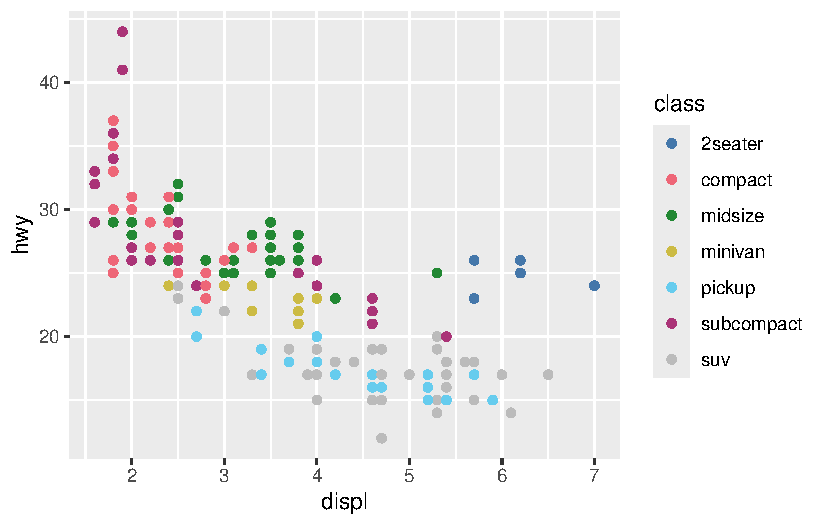
\includegraphics[keepaspectratio]{manipulation/couleurs_files/figure-pdf/unnamed-chunk-6-2.pdf}}

\begin{Shaded}
\begin{Highlighting}[]
\FunctionTok{plot\_scheme}\NormalTok{(}\FunctionTok{colour}\NormalTok{(}\StringTok{"muted"}\NormalTok{)(}\DecValTok{9}\NormalTok{), }\AttributeTok{colours =} \ConstantTok{TRUE}\NormalTok{)}
\end{Highlighting}
\end{Shaded}

\pandocbounded{\includegraphics[keepaspectratio]{manipulation/couleurs_files/figure-pdf/unnamed-chunk-7-1.pdf}}

\begin{Shaded}
\begin{Highlighting}[]
\FunctionTok{plot\_scheme}\NormalTok{(}\FunctionTok{colour}\NormalTok{(}\StringTok{"PRGn"}\NormalTok{)(}\DecValTok{9}\NormalTok{), }\AttributeTok{colours =} \ConstantTok{TRUE}\NormalTok{, }\AttributeTok{size =} \FloatTok{0.9}\NormalTok{)}
\end{Highlighting}
\end{Shaded}

\pandocbounded{\includegraphics[keepaspectratio]{manipulation/couleurs_files/figure-pdf/unnamed-chunk-8-1.pdf}}

Pour la liste complète des palettes disponibles, voir
\url{https://packages.tesselle.org/khroma/articles/tol.html}.

\subsection{\texorpdfstring{Interface unifiée avec
\texttt{\{paletteer\}}}{Interface unifiée avec \{paletteer\}}}\label{interface-unifiuxe9e-avec-paletteer}

L'extension \texttt{\{paletteer\}} vise à proposer une interface unifiée
pour l'utilisation de palettes de couleurs fournies par d'autres
packages (dont \texttt{\{khroma\}}, mais aussi par exemple
\texttt{\{ggsci\}} qui fournit les palettes utilisées par certaines
revues scientifiques). Plus de 2~500 palettes sont ainsi disponibles.

On peut afficher un aperçu des principales palettes disponibles dans
\texttt{\{paletteer\}} avec la commande suivante~:

\begin{Shaded}
\begin{Highlighting}[]
\NormalTok{gt}\SpecialCharTok{::}\FunctionTok{info\_paletteer}\NormalTok{()}
\end{Highlighting}
\end{Shaded}

Pour afficher la liste complète des palettes discrètes et continues, on
utilisera les commandes suivantes~:

\begin{Shaded}
\begin{Highlighting}[]
\NormalTok{palettes\_d\_names }\SpecialCharTok{|\textgreater{}} \FunctionTok{View}\NormalTok{()}
\NormalTok{palettes\_c\_names }\SpecialCharTok{|\textgreater{}} \FunctionTok{View}\NormalTok{()}
\end{Highlighting}
\end{Shaded}

La fonction \texttt{paletteer::paletteer\_d()} permet d'obtenir les
codes hexadécimaux d'une palette discrète en précisant le nombre de
couleurs attendues. Les fonctions
\texttt{paletteer::scale\_color\_paletteer\_d()} et
\texttt{paletteer::scale\_fill\_paletteer\_d()} permettront d'utiliser
une palette donnée avec \texttt{\{ggplot2\}}.

\begin{Shaded}
\begin{Highlighting}[]
\FunctionTok{library}\NormalTok{(paletteer)}
\FunctionTok{paletteer\_d}\NormalTok{(}\StringTok{"khroma::bright"}\NormalTok{, }\AttributeTok{n =} \DecValTok{5}\NormalTok{)}
\end{Highlighting}
\end{Shaded}

\begin{verbatim}
<colors>
#4477AAFF #EE6677FF #228833FF #CCBB44FF #66CCEEFF 
\end{verbatim}

\begin{Shaded}
\begin{Highlighting}[]
\FunctionTok{ggplot}\NormalTok{(mpg) }\SpecialCharTok{+}
  \FunctionTok{aes}\NormalTok{(}\AttributeTok{x =}\NormalTok{ displ, }\AttributeTok{y =}\NormalTok{ hwy, }\AttributeTok{colour =}\NormalTok{ class) }\SpecialCharTok{+}
  \FunctionTok{geom\_point}\NormalTok{() }\SpecialCharTok{+}
  \FunctionTok{scale\_color\_paletteer\_d}\NormalTok{(}\StringTok{"khroma::bright"}\NormalTok{)}
\end{Highlighting}
\end{Shaded}

\pandocbounded{\includegraphics[keepaspectratio]{manipulation/couleurs_files/figure-pdf/unnamed-chunk-11-1.pdf}}

L'équivalent existe pour les palettes continues, avec
\texttt{paletteer::paletteer\_c()},
\texttt{paletteer::scale\_color\_paletteer\_c()} et
\texttt{paletteer::scale\_fill\_paletteer\_c()} .

\begin{Shaded}
\begin{Highlighting}[]
\FunctionTok{paletteer\_c}\NormalTok{(}\StringTok{"viridis::viridis"}\NormalTok{, }\AttributeTok{n =} \DecValTok{6}\NormalTok{)}
\end{Highlighting}
\end{Shaded}

\begin{verbatim}
<colors>
#440154FF #414487FF #2A788EFF #22A884FF #7AD151FF #FDE725FF 
\end{verbatim}

\begin{Shaded}
\begin{Highlighting}[]
\FunctionTok{ggplot}\NormalTok{(iris) }\SpecialCharTok{+}
  \FunctionTok{aes}\NormalTok{(}\AttributeTok{x =}\NormalTok{ Sepal.Length, }\AttributeTok{y =}\NormalTok{ Sepal.Width, }\AttributeTok{colour =}\NormalTok{ Petal.Length) }\SpecialCharTok{+}
  \FunctionTok{geom\_point}\NormalTok{() }\SpecialCharTok{+}
  \FunctionTok{scale\_colour\_paletteer\_c}\NormalTok{(}\StringTok{"viridis::viridis"}\NormalTok{, }\AttributeTok{direction =} \SpecialCharTok{{-}}\DecValTok{1}\NormalTok{)}
\end{Highlighting}
\end{Shaded}

\pandocbounded{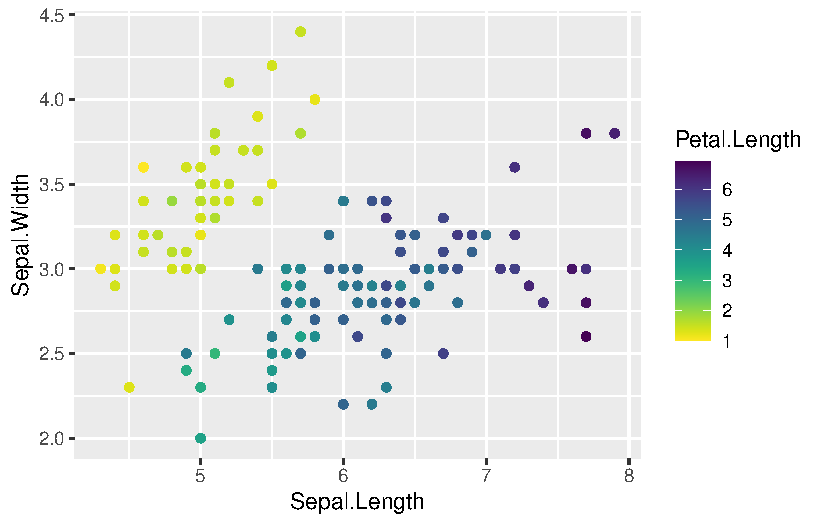
\includegraphics[keepaspectratio]{manipulation/couleurs_files/figure-pdf/unnamed-chunk-12-1.pdf}}

\part{\textbf{Analyses}}

\chapter{\texorpdfstring{Graphiques avec
\texttt{ggplot2}}{Graphiques avec ggplot2}}\label{sec-ggplot2}

Le package \texttt{\{ggplot2\}} fait partie intégrante du
\emph{tidyverse}. Développé par Hadley Wickham, ce package met en œuvre
la grammaire graphique théorisée par Leland Wilkinson. Il devient vite
indispensable lorsque l'on souhaite réaliser des graphiques un peu
complexe.

\section{Ressources}\label{ressources}

Il existe de très nombreuses ressources traitant de
\texttt{\{ggplot2\}}.

Pour une introduction en français, on pourra se référer au chapitre
\href{https://juba.github.io/tidyverse/08-ggplot2.html}{Visualiser avec
ggplot2} de l'\emph{Introduction à R et au tidyverse} de Julien Barnier,
au chapitre
\href{https://larmarange.github.io/analyse-R/intro-ggplot2.html}{Introduction
à ggplot2, la grammaire des graphiques} du site \emph{analyse-R} et
adapté d'une séance de cours de François Briatte, ou encore au chapitre
\href{http://egallic.fr/Enseignement/R/m1_stat_eco_logiciel_R.pdf}{Graphiques}
du cours \emph{Logiciel R et programmation} d'Ewen Gallic.

Pour les anglophones, la référence reste encore l'ouvrage \emph{ggplot2:
Elegant Graphics for Data Analysis} d'Hadley Wickham lui-même, dont la
troisième édition est librement accessible en ligne
(\url{https://ggplot2-book.org/}). D'un point de vue pratique, l'ouvrage
\emph{R Graphics Cookbook: practical recipes for visualizing data} de
Winston Chang est une mine d'informations, ouvrage là encore librement
accessible en ligne (\url{https://r-graphics.org/}).

\section{\texorpdfstring{Les bases de
\texttt{ggplot2}}{Les bases de ggplot2}}\label{les-bases-de-ggplot2}

\texttt{\{ggplot2\}} nécessite que les données du graphique soient sous
la forme d'un tableau de données (\emph{data.frame} ou \emph{tibble}) au
format \emph{tidy}, c'est-à-dire avec une ligne par observation et les
différentes valeurs à représenter sous forme de variables du tableau.

\begin{figure}

\centering{

\pandocbounded{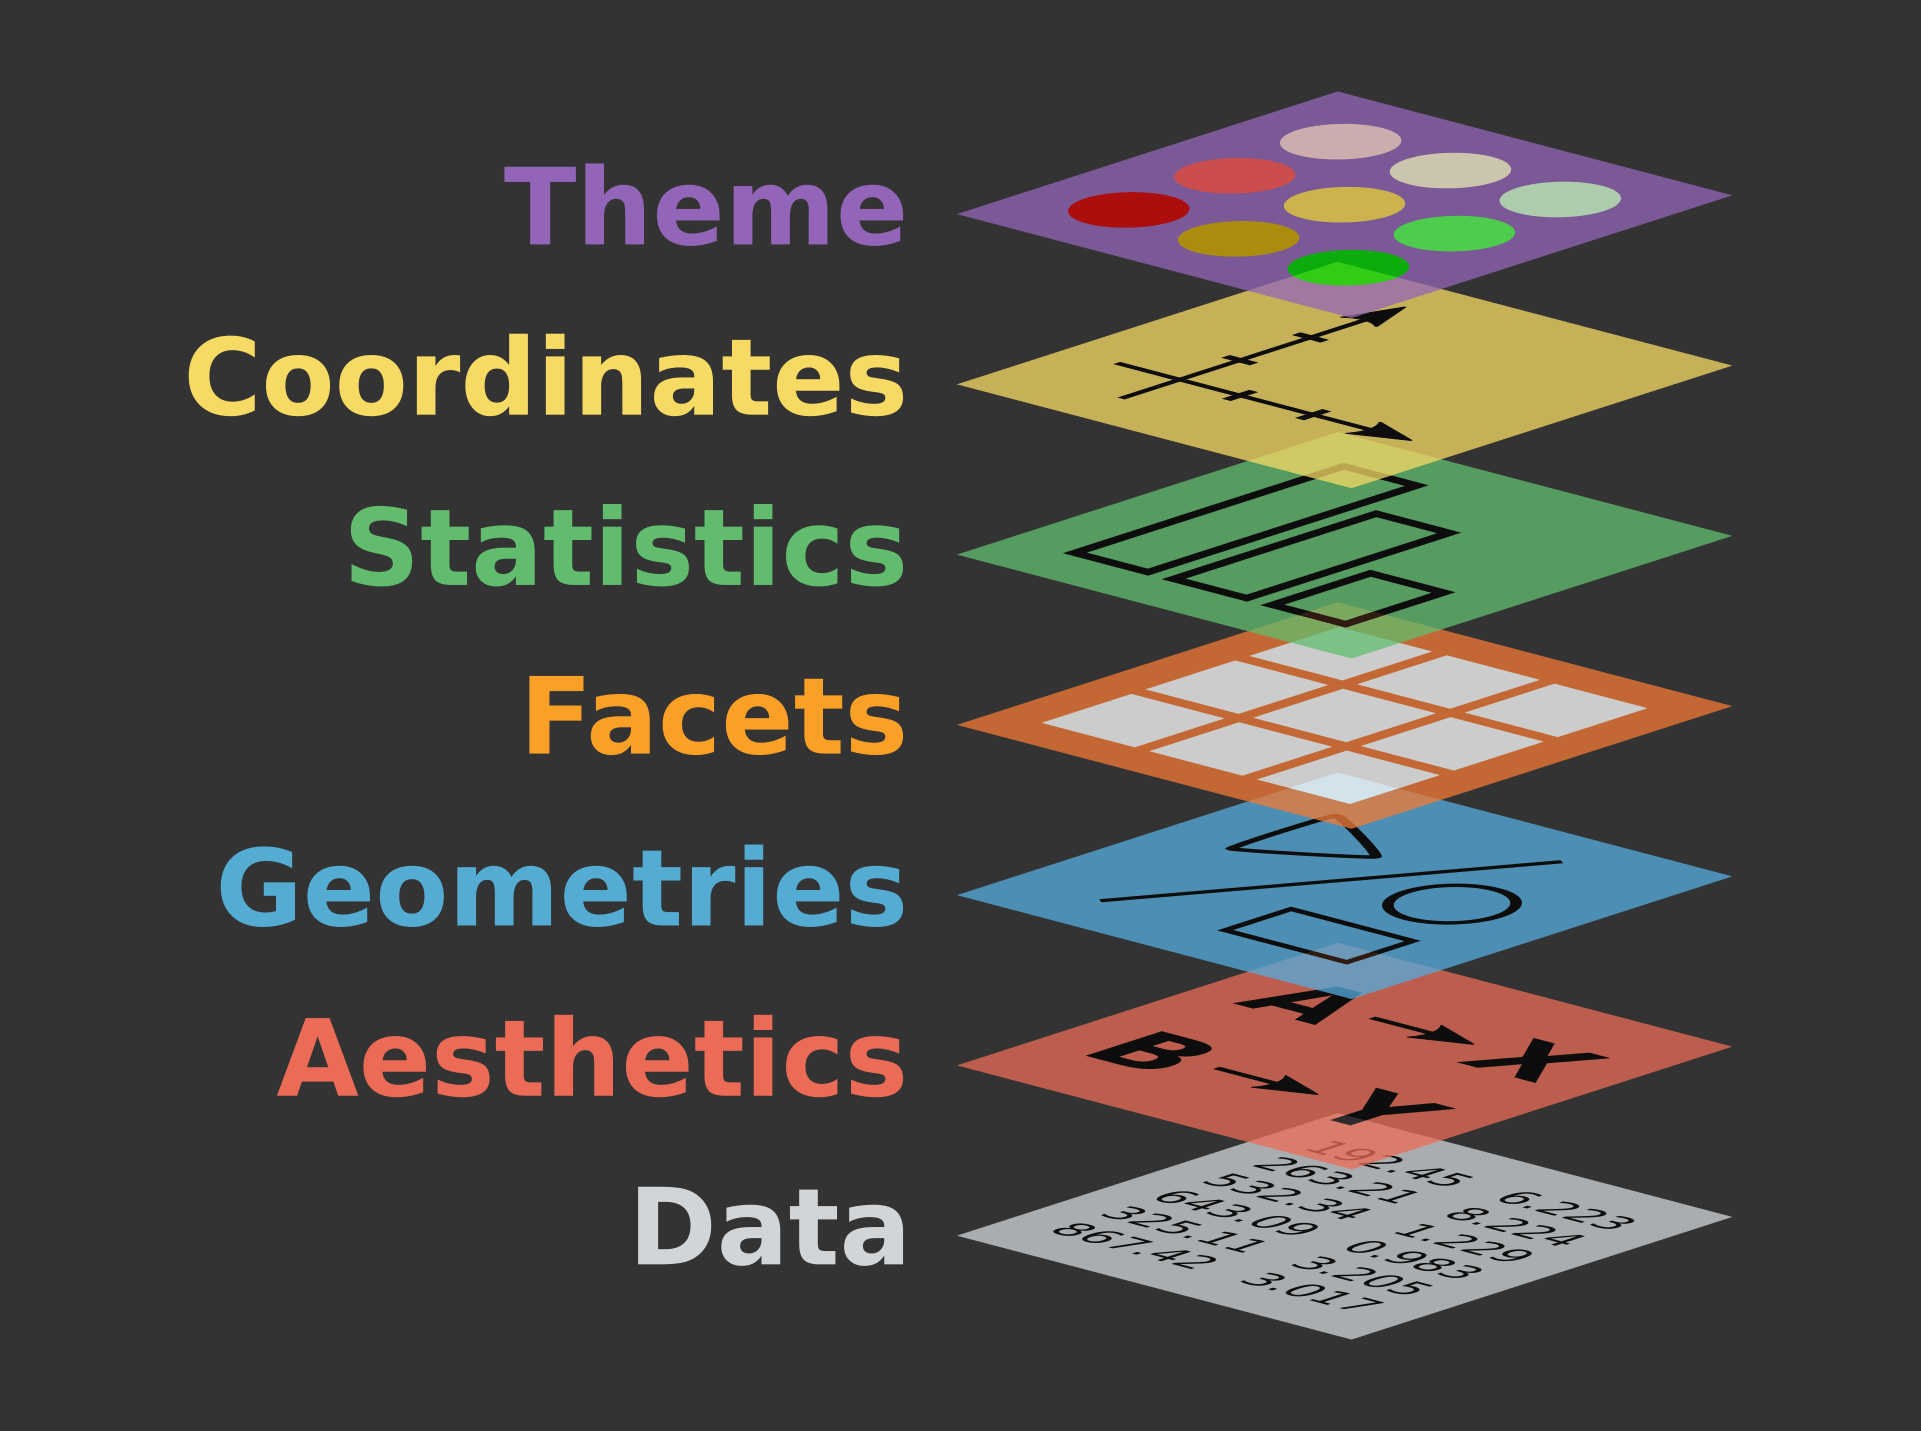
\includegraphics[keepaspectratio]{analyses/ressources/ggplot-grammar-of-graphics.png}}

}

\caption{\label{fig-grammaire-graphiques}La grammaire des graphiques}

\end{figure}%

Tous les graphiques avec \texttt{\{ggplot2\}} suivent une même logique.
En \textbf{premier} lieu, on appellera la fonction
\texttt{ggplot2::ggplot()} en lui passant en paramètre le fichier de
données.

\texttt{\{ggplot2\}} nomme \emph{esthétiques} les différentes propriétés
visuelles d'un graphique, à savoir l'axe des x (\texttt{x}), celui des y
(\texttt{y}), la couleur des lignes (\texttt{colour}), celle de
remplissage des polygones (\texttt{fill}), le type de lignes
(\texttt{linetype}), la forme des points (\texttt{shape}), etc. Une
représentation graphique consiste donc à représenter chacune de nos
variables d'intérêt selon une esthétique donnée. En \textbf{second}
lieu, on appellera donc la fonction \texttt{ggplot2::aes()} pour
indiquer la correspondance entre les variables de notre fichier de
données et les esthétiques du graphique.

A minima, il est nécessaire d'indiquer en \textbf{troisième} lieu une
\emph{géométrie}, autrement dit la manière dont les éléments seront
représentés visuellement. À chaque géométrie corresponds une fonction
commençant par \texttt{geom\_}, par exemple
\texttt{ggplot2::geom\_point()} pour dessiner des points,
\texttt{ggplot2::geom\_line()} pour des lignes,
\texttt{ggplot2::geom\_bar()} pour des barres ou encore
\texttt{ggplot2::geom\_area()} pour des aires. Il existe de nombreuses
géométries différentes\footnote{On trouvera une liste dans la
  \emph{cheat sheet} de \texttt{\{ggplot2\}}, voir
  Section~\ref{sec-cheatsheet-ggplot2}.}, chacune prenant en compte
certaines esthétiques, certaines étant requises pour cette géométrie et
d'autres optionnelles. La liste des esthétiques prises en compte par
chaque géométrie est indiquée dans l'aide en ligne de cette dernière.

Voici un exemple minimal de graphique avec \texttt{\{ggplot2\}}~:

\begin{Shaded}
\begin{Highlighting}[]
\FunctionTok{library}\NormalTok{(ggplot2)}
\NormalTok{p }\OtherTok{\textless{}{-}} 
  \FunctionTok{ggplot}\NormalTok{(iris) }\SpecialCharTok{+}
  \FunctionTok{aes}\NormalTok{(}
    \AttributeTok{x =}\NormalTok{ Petal.Length, }
    \AttributeTok{y =}\NormalTok{ Petal.Width, }
    \AttributeTok{colour =}\NormalTok{ Species}
\NormalTok{  ) }\SpecialCharTok{+}
  \FunctionTok{geom\_point}\NormalTok{()}
\NormalTok{p}
\end{Highlighting}
\end{Shaded}

\begin{figure}[H]

\centering{

\pandocbounded{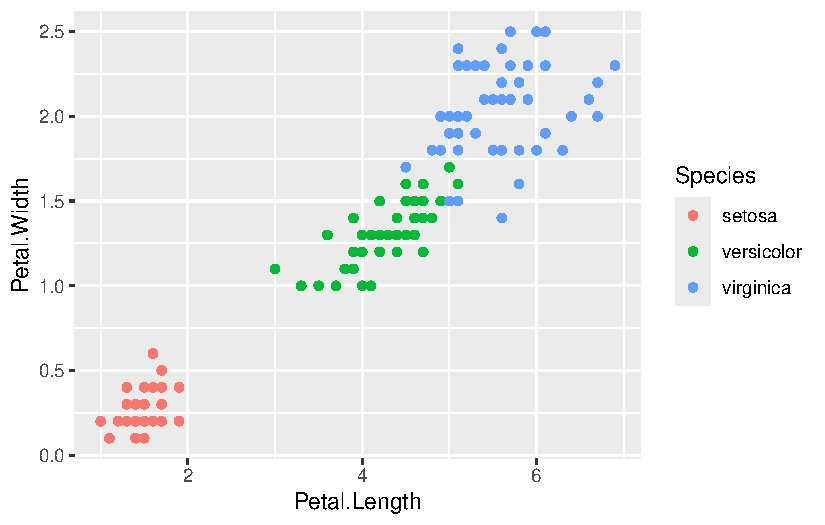
\includegraphics[keepaspectratio]{analyses/ggplot2_files/figure-pdf/fig-exemple-simple-ggplot2-1.pdf}}

}

\caption{\label{fig-exemple-simple-ggplot2}Un exemple simple de nuage de
points avec \texttt{ggplot2}}

\end{figure}%

\begin{tcolorbox}[enhanced jigsaw, toptitle=1mm, bottomtitle=1mm, colframe=quarto-callout-important-color-frame, toprule=.15mm, left=2mm, bottomrule=.15mm, opacitybacktitle=0.6, opacityback=0, coltitle=black, breakable, rightrule=.15mm, arc=.35mm, title=\textcolor{quarto-callout-important-color}{\faExclamation}\hspace{0.5em}{Syntaxe additive}, colbacktitle=quarto-callout-important-color!10!white, titlerule=0mm, leftrule=.75mm, colback=white]

Le développement de \texttt{\{ggplot2\}} a débuté avant celui du
\emph{tidyverse} et la généralisation du \emph{pipe}. Dès lors, on ne
sera pas étonné que la syntaxe de \texttt{\{ggplot2\}} n'ait pas recours
à ce dernier mais repose sur une approche \emph{additive}. Un graphique
est dès lors initialisé avec la fonction \texttt{ggplot2::ggplot()} et
l'on ajoutera successivement des éléments au graphique en appelant
différentes fonctions et en utilisant l'opérateur \texttt{+}.

\end{tcolorbox}

Il est ensuite possible de personnaliser de nombreux éléments d'un
graphique et notamment~:

\begin{itemize}
\tightlist
\item
  les \emph{étiquettes} ou \emph{labs} (titre, axes, légendes) avec
  \texttt{ggplot2::ggtitle()}, \texttt{ggplot2::xlab()},
  \texttt{ggplot2::ylab()} ou encore la fonction plus générique
  \texttt{ggplot2::labs()}~;
\item
  les \emph{échelles} (\emph{scales}) des différentes esthétiques avec
  les fonctions commençant par \texttt{scale\_}~;
\item
  le système de \emph{coordonnées} avec les fonctions commençant par
  \texttt{coord\_}~;
\item
  les \emph{facettes} (\emph{facets}) avec les fonctions commençant par
  \texttt{facet\_}~;
\item
  la \emph{légende} (\emph{guides}) avec les fonctions commençant par
  \texttt{guide\_}~;
\item
  le \emph{thème} du graphiques (mise en forme des différents éléments)
  avec \texttt{ggplot2::theme()}.
\end{itemize}

\begin{Shaded}
\begin{Highlighting}[]
\NormalTok{p }\SpecialCharTok{+}
  \FunctionTok{labs}\NormalTok{(}
    \AttributeTok{x =} \StringTok{"Longueur du pétale"}\NormalTok{,}
    \AttributeTok{y =} \StringTok{"Largeur du pétale"}\NormalTok{,}
    \AttributeTok{colour =} \StringTok{"Espèce"}
\NormalTok{  ) }\SpecialCharTok{+}
  \FunctionTok{ggtitle}\NormalTok{(}
    \StringTok{"Relation entre longueur et largeur des pétales"}\NormalTok{,}
    \AttributeTok{subtitle =} \StringTok{"Jeu de données Iris"}
\NormalTok{  ) }\SpecialCharTok{+}
  \FunctionTok{scale\_x\_continuous}\NormalTok{(}\AttributeTok{breaks =} \DecValTok{1}\SpecialCharTok{:}\DecValTok{7}\NormalTok{) }\SpecialCharTok{+}
  \FunctionTok{scale\_y\_continuous}\NormalTok{(}
    \AttributeTok{labels =}\NormalTok{ scales}\SpecialCharTok{::}\FunctionTok{label\_number}\NormalTok{(}\AttributeTok{decimal.mark =} \StringTok{","}\NormalTok{)}
\NormalTok{  ) }\SpecialCharTok{+}
  \FunctionTok{coord\_equal}\NormalTok{() }\SpecialCharTok{+}
  \FunctionTok{facet\_grid}\NormalTok{(}\AttributeTok{cols =} \FunctionTok{vars}\NormalTok{(Species)) }\SpecialCharTok{+}
  \FunctionTok{guides}\NormalTok{(}
    \AttributeTok{color =} \FunctionTok{guide\_legend}\NormalTok{(}\AttributeTok{nrow =} \DecValTok{2}\NormalTok{)}
\NormalTok{  ) }\SpecialCharTok{+}
  \FunctionTok{theme\_light}\NormalTok{() }\SpecialCharTok{+}
  \FunctionTok{theme}\NormalTok{(}
    \AttributeTok{legend.position =} \StringTok{"bottom"}\NormalTok{,}
    \AttributeTok{axis.title =} \FunctionTok{element\_text}\NormalTok{(}\AttributeTok{face =} \StringTok{"bold"}\NormalTok{)}
\NormalTok{  )}
\end{Highlighting}
\end{Shaded}

\begin{figure}[H]

\centering{

\pandocbounded{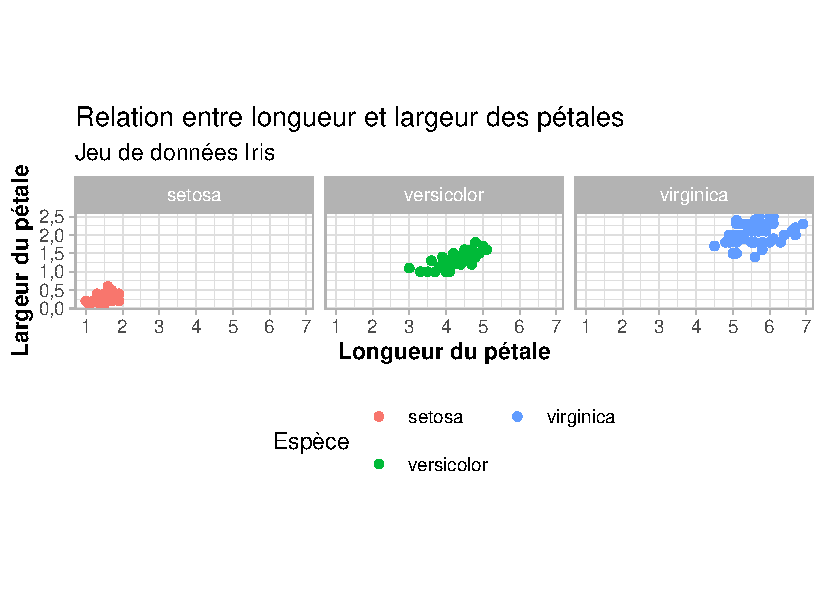
\includegraphics[keepaspectratio]{analyses/ggplot2_files/figure-pdf/fig-exemple-avance-ggplot2-1.pdf}}

}

\caption{\label{fig-exemple-avance-ggplot2}Un exemple avancé de nuage de
points avec \texttt{ggplot2}}

\end{figure}%

Pour visualiser chaque étape du code, vous pouvez consulter le diaporama
suivant~:
\url{https://larmarange.github.io/guide-R/analyses/ressources/flipbook-ggplot2.html}

\section{Cheatsheet}\label{sec-cheatsheet-ggplot2}

\begin{figure}

\centering{

\href{https://github.com/rstudio/cheatsheets/raw/main/data-visualization-2.1.pdf}{\pandocbounded{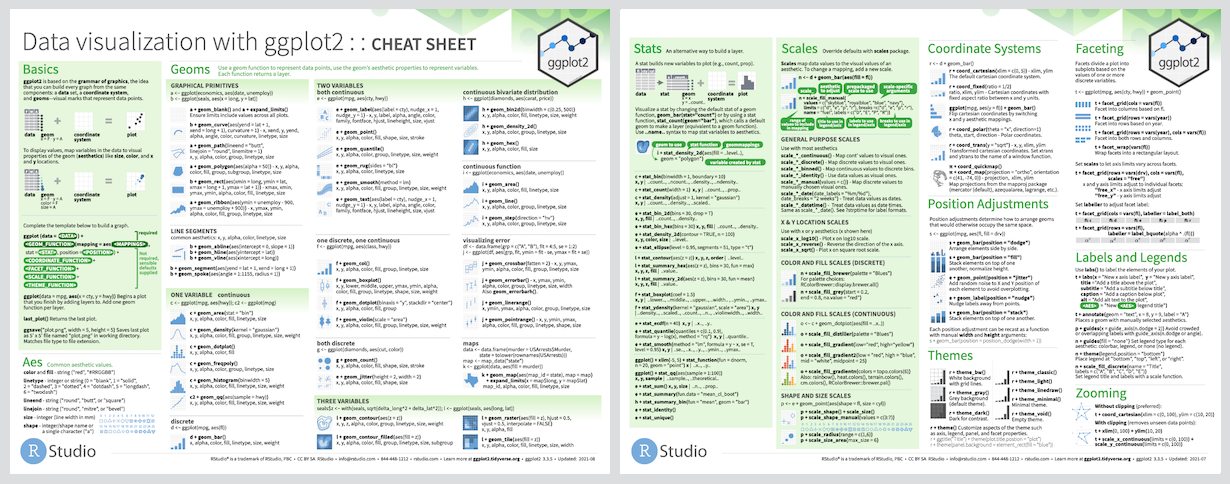
\includegraphics[keepaspectratio]{analyses/ressources/data-visualization-cheatsheet-thumbs.png}}}

}

\caption{\label{fig-cheatsheet-ggplot2}Cheatsheet ggplot2}

\end{figure}%

\section{\texorpdfstring{Exploration visuelle avec
\texttt{esquisse}}{Exploration visuelle avec esquisse}}\label{sec-esquisse}

Le package \texttt{\{esquisse\}} propose un \emph{addin} offrant une
interface visuelle pour la création de graphiques \texttt{\{ggplot2\}}.
Après installation du package, on pourra lancer \texttt{\{esquisse\}}
directement à partir du menu \emph{addins} de \textbf{RStudio}.

\begin{figure}

\centering{

\pandocbounded{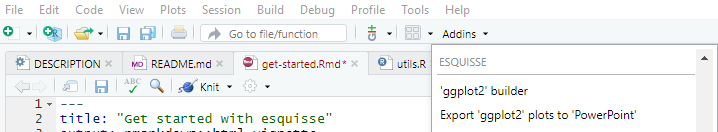
\includegraphics[keepaspectratio]{analyses/ressources/esquisse-launch-addin.png}}

}

\caption{\label{fig-lancement-esquisse}Lancement d'\texttt{esquisse} à
partir du menu \emph{Addins} de \textbf{RStudio}}

\end{figure}%

Au lancement de l'\emph{addin}, une interface permettra de choisir le
tableau de données à partir duquel générer le graphique. Le plus simple
est de choisir un tableau présent dans l'environnement. Mais
\texttt{\{esquisse\}} offre aussi la possibilité d'importer des fichiers
externes, voir de procéder à quelques modifications des données.

\begin{figure}

\centering{

\pandocbounded{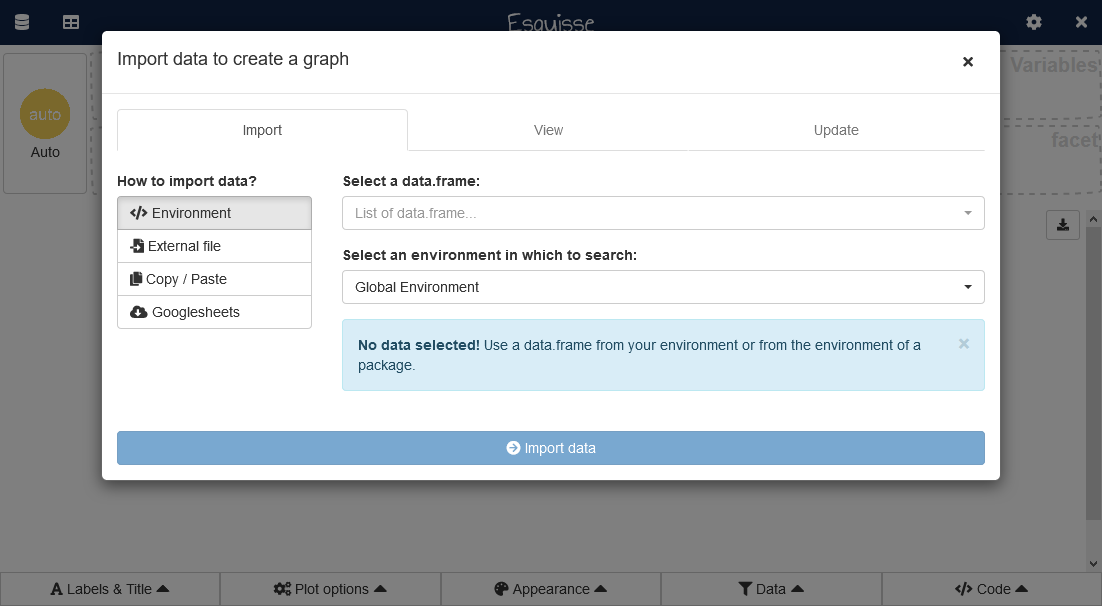
\includegraphics[keepaspectratio]{analyses/ressources/esquisse-import-data.png}}

}

\caption{\label{fig-esquisse-import-donnees}Import de données au
lancement d'\texttt{esquisse}}

\end{figure}%

Le principe général d'\texttt{\{esquisse\}} consiste à associer des
variables à des esthétiques par glisser/déposer\footnote{Si une
  esthétique n'est pas visible à l'écran, on pourra cliquer en haut à
  droite sur l'icône en forme de roue dentée afin de choisir d'afficher
  plus d'esthétiques.}. L'outil déterminera automatiquement une
géométrie adaptée en fonction de la nature des variables (continues ou
catégorielles). Un clic sur le nom de la géométrie en haut à gauche
permet de sélectionner une autre géométrie.

\begin{figure}

\centering{

\pandocbounded{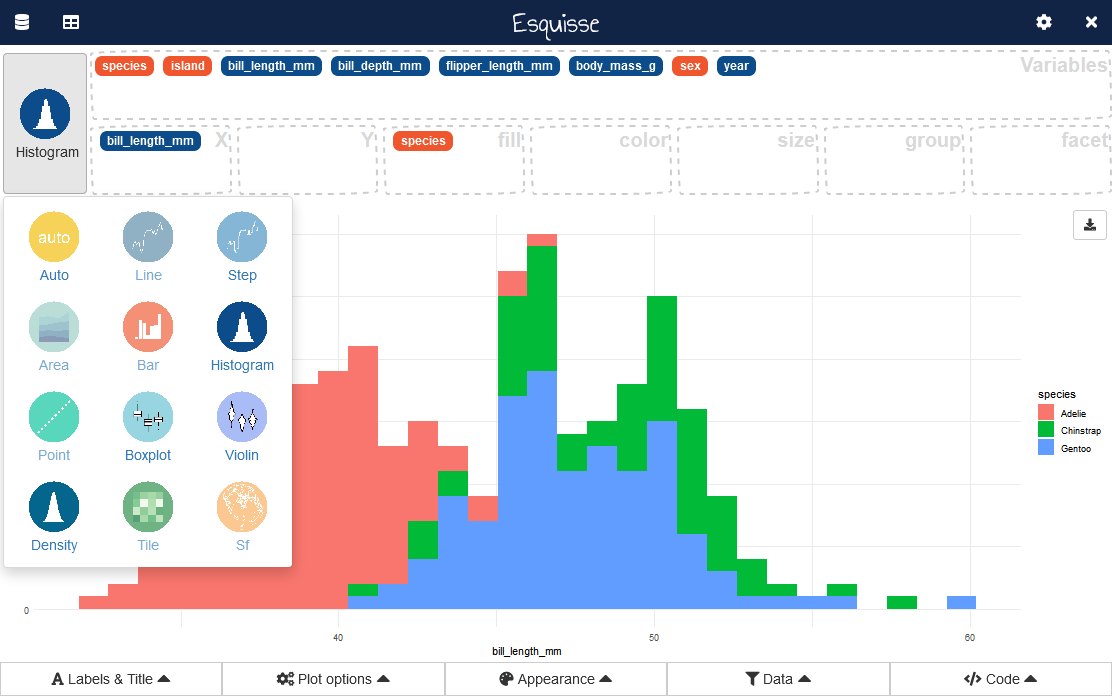
\includegraphics[keepaspectratio]{analyses/ressources/esquisse-geometries.png}}

}

\caption{\label{fig-esquisse-géométrie}Choix d'une géométrie dans
\texttt{esquisse}}

\end{figure}%

Les menus situés en bas de l'écran permettent d'ajouter/modifier des
étiquettes, de modifier certaines options du graphiques, de modifier les
échelles de couleurs et l'apparence du graphique, et de filtrer les
observations inclues dans le graphique.

Le menu \textbf{Code} permet de récupérer le code correspondant au
graphique afin de pouvoir le copier/coller dans un script.

\begin{figure}

\centering{

\pandocbounded{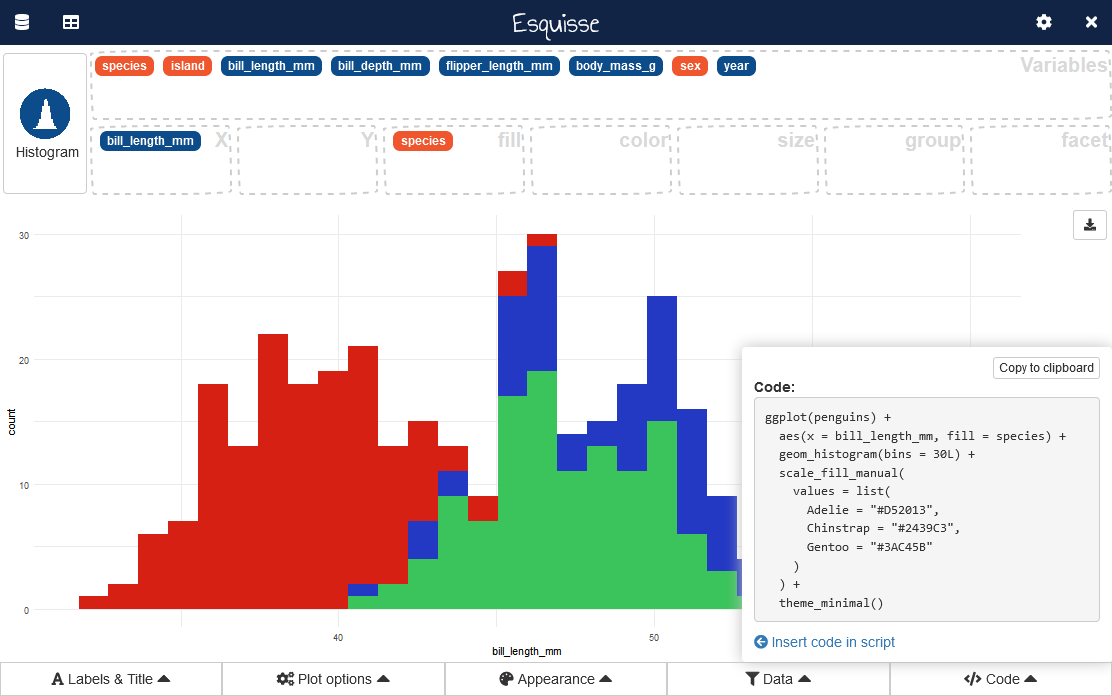
\includegraphics[keepaspectratio]{analyses/ressources/esquisse-controls-code.png}}

}

\caption{\label{fig-esquisse-code}Obtenir le code du graphique obtenu
avec \texttt{esquisse}}

\end{figure}%

\texttt{\{esquisse\}} offre également la possibilité d'exporter le
graphique obtenu dans différents formats.

\section{webin-R}\label{webin-r-4}

L'utilisation d'\texttt{\{esquisse\}} est présentée dans le webin-R \#03
(\emph{statistiques descriptives avec gtsummary et esquisse}) sur
\href{https://youtu.be/oEF_8GXyP5c?t=2620}{YouTube}.

\url{https://youtu.be/oEF_8GXyP5c}

\texttt{\{ggplot2\}} est abordé plus en détails dans le webin-R \#08
(\emph{ggplot2 et la grammaire des graphiques}) sur
\href{https://youtu.be/msnwENny_cg}{YouTube}.

\url{https://youtu.be/msnwENny_cg}

\section{Combiner plusieurs graphiques}\label{sec-combiner-graphiques}

Plusieurs packages proposent des fonctions pour combiner ensemble des
graphiques \texttt{\{ggplot2\}}, comme \texttt{\{patchwork\}},
\texttt{\{ggpubr\}}, \texttt{\{egg\}} ou \texttt{\{cowplot\}}. Ici, nous
privilégierons le package \texttt{\{patchwork\}} car, bien qu'il ne
fasse pas partie du \emph{tidyverse}, est développé et maintenant par
les mêmes auteurs que \texttt{\{ggplot2\}}.

Commençons par créer quelques graphiques avec \texttt{\{ggplot2\}}.

\begin{Shaded}
\begin{Highlighting}[]
\NormalTok{p1 }\OtherTok{\textless{}{-}} \FunctionTok{ggplot}\NormalTok{(mtcars) }\SpecialCharTok{+}
  \FunctionTok{aes}\NormalTok{(}\AttributeTok{x =}\NormalTok{ wt, }\AttributeTok{y =}\NormalTok{ mpg) }\SpecialCharTok{+} 
  \FunctionTok{geom\_point}\NormalTok{()}
\NormalTok{p2 }\OtherTok{\textless{}{-}} \FunctionTok{ggplot}\NormalTok{(mtcars) }\SpecialCharTok{+}
  \FunctionTok{aes}\NormalTok{(}\AttributeTok{x =} \FunctionTok{factor}\NormalTok{(cyl)) }\SpecialCharTok{+}
  \FunctionTok{geom\_bar}\NormalTok{()}
\NormalTok{p3 }\OtherTok{\textless{}{-}} \FunctionTok{ggplot}\NormalTok{(mtcars) }\SpecialCharTok{+}
  \FunctionTok{aes}\NormalTok{(}\AttributeTok{x =} \FunctionTok{factor}\NormalTok{(cyl), }\AttributeTok{y =}\NormalTok{ mpg) }\SpecialCharTok{+}
  \FunctionTok{geom\_violin}\NormalTok{() }\SpecialCharTok{+}
  \FunctionTok{theme}\NormalTok{(}\AttributeTok{axis.title =} \FunctionTok{element\_text}\NormalTok{(}\AttributeTok{size =} \DecValTok{20}\NormalTok{))}
\NormalTok{p4 }\OtherTok{\textless{}{-}} \FunctionTok{ggplot}\NormalTok{(mtcars) }\SpecialCharTok{+}
  \FunctionTok{aes}\NormalTok{(}\AttributeTok{x =} \FunctionTok{factor}\NormalTok{(cyl), }\AttributeTok{y =}\NormalTok{ mpg) }\SpecialCharTok{+} 
  \FunctionTok{geom\_boxplot}\NormalTok{() }\SpecialCharTok{+}
  \FunctionTok{ylab}\NormalTok{(}\ConstantTok{NULL}\NormalTok{)}
\end{Highlighting}
\end{Shaded}

Le symbole \texttt{+} permet de combiner des graphiques entre eux. Le
package \texttt{\{patchwork\}} déterminera le nombre de lignes et de
colonnes en fonction du nombre de graphiques. On pourra noter que les
axes des graphiques sont alignés les uns par rapports aux autres.

\begin{Shaded}
\begin{Highlighting}[]
\FunctionTok{library}\NormalTok{(patchwork)}
\NormalTok{p1 }\SpecialCharTok{+}\NormalTok{ p2 }\SpecialCharTok{+}\NormalTok{ p3 }\SpecialCharTok{+}\NormalTok{ p4}
\end{Highlighting}
\end{Shaded}

\pandocbounded{\includegraphics[keepaspectratio]{analyses/ggplot2_files/figure-pdf/unnamed-chunk-4-1.pdf}}

Les symboles \texttt{\textbar{}} et \texttt{/} permettent d'indiquer une
disposition côte à côte ou les uns au-dessus des autres.

\begin{Shaded}
\begin{Highlighting}[]
\NormalTok{p1 }\SpecialCharTok{|}\NormalTok{ p2 }\SpecialCharTok{|}\NormalTok{ p3}
\end{Highlighting}
\end{Shaded}

\pandocbounded{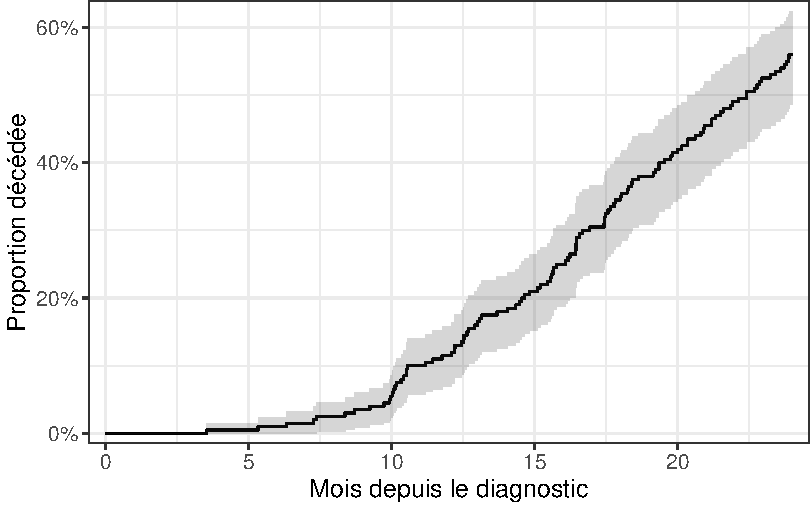
\includegraphics[keepaspectratio]{analyses/ggplot2_files/figure-pdf/unnamed-chunk-5-1.pdf}}

\begin{Shaded}
\begin{Highlighting}[]
\NormalTok{p1 }\SpecialCharTok{/}\NormalTok{ p2}
\end{Highlighting}
\end{Shaded}

\pandocbounded{\includegraphics[keepaspectratio]{analyses/ggplot2_files/figure-pdf/unnamed-chunk-6-1.pdf}}

On peut utiliser les parenthèses pour indiquer des arrangements plus
complexes.

\begin{Shaded}
\begin{Highlighting}[]
\NormalTok{(p1 }\SpecialCharTok{+}\NormalTok{ p2) }\SpecialCharTok{/}\NormalTok{ p3}
\end{Highlighting}
\end{Shaded}

\pandocbounded{\includegraphics[keepaspectratio]{analyses/ggplot2_files/figure-pdf/unnamed-chunk-7-1.pdf}}

\begin{Shaded}
\begin{Highlighting}[]
\NormalTok{(p1 }\SpecialCharTok{+}\NormalTok{ p2) }\SpecialCharTok{|}\NormalTok{ p3}
\end{Highlighting}
\end{Shaded}

\pandocbounded{\includegraphics[keepaspectratio]{analyses/ggplot2_files/figure-pdf/unnamed-chunk-8-1.pdf}}

Si l'on a une liste de graphiques, on pourra appeler
\texttt{patchwork::wrap\_plots()}.

\begin{Shaded}
\begin{Highlighting}[]
\FunctionTok{list}\NormalTok{(p1, p2, p3, p4) }\SpecialCharTok{|\textgreater{}} 
  \FunctionTok{wrap\_plots}\NormalTok{()}
\end{Highlighting}
\end{Shaded}

\pandocbounded{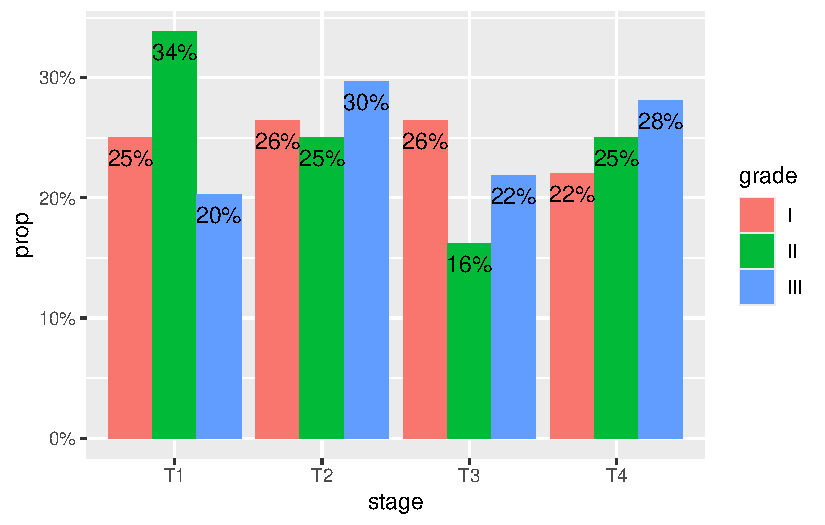
\includegraphics[keepaspectratio]{analyses/ggplot2_files/figure-pdf/unnamed-chunk-9-1.pdf}}

La fonction \texttt{patchwork::plot\_layout()} permet de contrôler les
hauteurs / largeurs relatives des lignes / colonnes.

\begin{Shaded}
\begin{Highlighting}[]
\NormalTok{p1 }\SpecialCharTok{+}\NormalTok{ p2 }\SpecialCharTok{+}\NormalTok{ p3 }\SpecialCharTok{+}\NormalTok{ p4 }\SpecialCharTok{+} \FunctionTok{plot\_layout}\NormalTok{(}\AttributeTok{widths =} \FunctionTok{c}\NormalTok{(}\DecValTok{2}\NormalTok{, }\DecValTok{1}\NormalTok{))}
\end{Highlighting}
\end{Shaded}

\pandocbounded{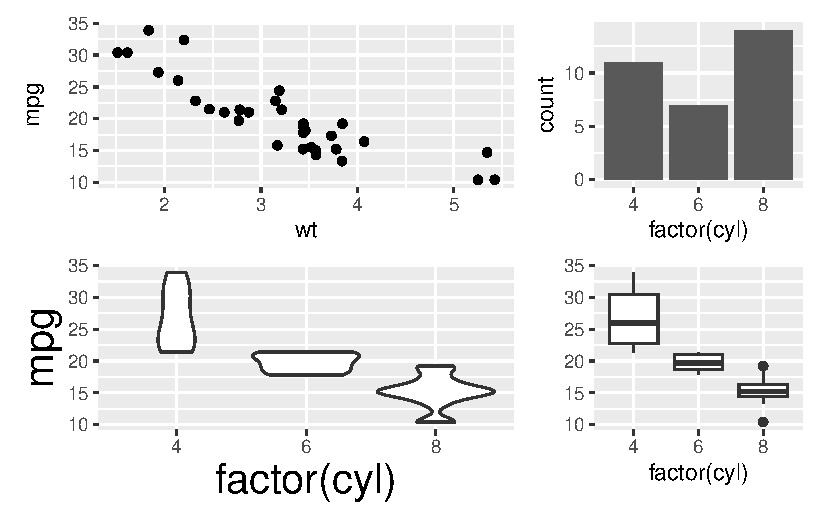
\includegraphics[keepaspectratio]{analyses/ggplot2_files/figure-pdf/unnamed-chunk-10-1.pdf}}

On peut également ajouter un titre ou des étiquettes avec
\texttt{patchwork::plot\_annotation()}.

\begin{Shaded}
\begin{Highlighting}[]
\NormalTok{p1 }\SpecialCharTok{+}\NormalTok{ p2 }\SpecialCharTok{+}\NormalTok{ p3 }\SpecialCharTok{+}\NormalTok{ p4 }\SpecialCharTok{+}
  \FunctionTok{plot\_annotation}\NormalTok{(}
    \AttributeTok{title =} \StringTok{"Titre du graphique"}\NormalTok{,}
    \AttributeTok{subtitle =} \StringTok{"sous{-}titre"}\NormalTok{,}
    \AttributeTok{caption =} \StringTok{"notes additionelles"}\NormalTok{,}
    \AttributeTok{tag\_levels =} \StringTok{"a"}\NormalTok{,}
    \AttributeTok{tag\_suffix =} \StringTok{"."}
\NormalTok{  )}
\end{Highlighting}
\end{Shaded}

\pandocbounded{\includegraphics[keepaspectratio]{analyses/ggplot2_files/figure-pdf/unnamed-chunk-11-1.pdf}}

\chapter{Statistique univariée \& Intervalles de
confiance}\label{sec-statistique-univariee}

On entend par statistique univariée l'étude d'une seule variable, que
celle-ci soit continue (quantitative) ou catégorielle (qualitative). La
statistique univariée fait partie de la statistique descriptive.

\section{Exploration graphique}\label{exploration-graphique}

Une première approche consiste à explorer visuelle la variable
d'intérêt, notamment à l'aide de l'interface proposée par
\texttt{\{esquisse\}} (cf Section~\ref{sec-esquisse}).

Nous indiquons ci-après le code correspond aux graphiques
\texttt{\{ggplot2\}} les plus courants.

\begin{Shaded}
\begin{Highlighting}[]
\FunctionTok{library}\NormalTok{(ggplot2)}
\end{Highlighting}
\end{Shaded}

\subsection{Variable continue}\label{variable-continue}

Un histogramme est la représentation graphique la plus commune pour
représenter la distribution d'une variable, par exemple ici la longueur
des pétales (variable \texttt{Petal.Length}) du fichier de données
\texttt{datasets::iris}. Il s'obtient avec la géométrie
\texttt{ggplot2::geom\_histogram()}.

\begin{Shaded}
\begin{Highlighting}[]
\FunctionTok{ggplot}\NormalTok{(iris) }\SpecialCharTok{+}
  \FunctionTok{aes}\NormalTok{(}\AttributeTok{x =}\NormalTok{ Petal.Length) }\SpecialCharTok{+}
  \FunctionTok{geom\_histogram}\NormalTok{()}
\end{Highlighting}
\end{Shaded}

\begin{verbatim}
`stat_bin()` using `bins = 30`. Pick better value with `binwidth`.
\end{verbatim}

\begin{figure}[H]

\centering{

\pandocbounded{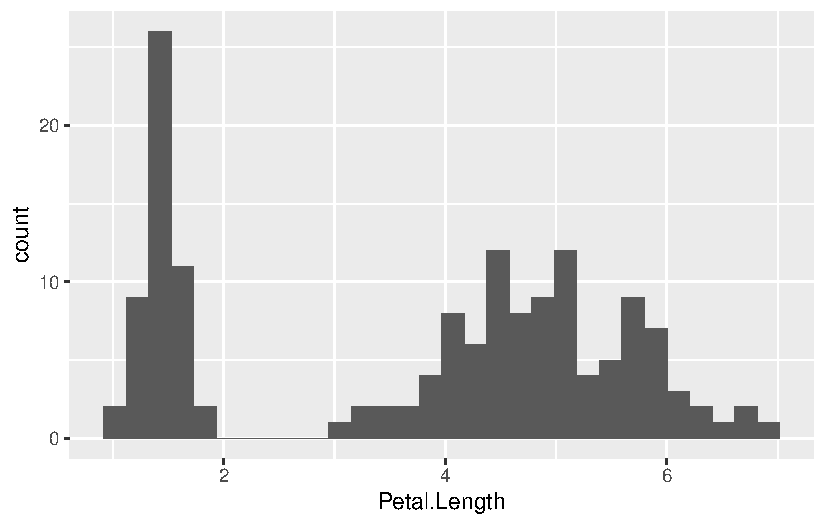
\includegraphics[keepaspectratio]{analyses/statistique-univariee_files/figure-pdf/fig-histogramme-simple-1.pdf}}

}

\caption{\label{fig-histogramme-simple}un histogramme simple}

\end{figure}%

\begin{tcolorbox}[enhanced jigsaw, toptitle=1mm, bottomtitle=1mm, colframe=quarto-callout-tip-color-frame, toprule=.15mm, left=2mm, bottomrule=.15mm, opacitybacktitle=0.6, opacityback=0, coltitle=black, breakable, rightrule=.15mm, arc=.35mm, title=\textcolor{quarto-callout-tip-color}{\faLightbulb}\hspace{0.5em}{Astuce}, colbacktitle=quarto-callout-tip-color!10!white, titlerule=0mm, leftrule=.75mm, colback=white]

Il faut noter qu'il nous a suffit d'associer simplement la variable
\texttt{Petal.Length} à l'esthétique \textbf{x}, sans avoir eu besoin
d'indiquer une variable pour l'esthétique \textbf{y}.

En fait, \texttt{\{ggplot2\}} associe par défaut à toute géométrie une
certaine statistique. Dans le cas de
\texttt{ggplot2::geom\_histogram()}, il s'agit de la statistique
\texttt{ggplot2::stat\_bin()} qui divise la variable continue en classes
de même largeur et compte le nombre d'observation dans chacune.
\texttt{ggplot2::stat\_bin()} renvoie un certain nombre de variables
calculées (la liste complète est indiquée dans la documentation dans la
section \emph{Compute variables}), dont la variable \texttt{count} qui
correspond au nombre d'observations la classe. On peut associer cette
variable calculée à une esthétique grâce à la fonction
\texttt{ggplot2::after\_stat()}, par exemple
\texttt{aes(y\ =\ after\_stat(count))}. Dans le cas présent, ce n'est
pas nécessaire car \texttt{\{ggplot2\}} fait cette association
automatiquement si l'on n'a pas déjà attribué une variable à
l'esthétique \textbf{y}.

\end{tcolorbox}

On peut personnaliser la couleur de remplissage des rectangles en
indiquant une valeur fixe pour l'esthétique \texttt{fill} dans l'appel
de \texttt{ggplot2::geom\_histogram()} (et non via la fonction
\texttt{ggplot2::aes()} puisqu'il ne s'agit pas d'une variable du
tableau de données). L'esthétique \texttt{colour} permet de spécifier la
couleur du trait des rectangles. Enfin, le paramètre \texttt{binwidth}
permet de spécifier la largeur des barres.

\begin{Shaded}
\begin{Highlighting}[]
\FunctionTok{ggplot}\NormalTok{(iris) }\SpecialCharTok{+}
  \FunctionTok{aes}\NormalTok{(}\AttributeTok{x =}\NormalTok{ Petal.Length) }\SpecialCharTok{+}
  \FunctionTok{geom\_histogram}\NormalTok{(}
    \AttributeTok{fill =}\StringTok{"lightblue"}\NormalTok{, }
    \AttributeTok{colour =} \StringTok{"black"}\NormalTok{, }
    \AttributeTok{binwidth =} \DecValTok{1}
\NormalTok{  ) }\SpecialCharTok{+}
  \FunctionTok{xlab}\NormalTok{(}\StringTok{"Longeur du pétale"}\NormalTok{) }\SpecialCharTok{+}
  \FunctionTok{ylab}\NormalTok{(}\StringTok{"Effectifs"}\NormalTok{)}
\end{Highlighting}
\end{Shaded}

\begin{figure}[H]

\centering{

\pandocbounded{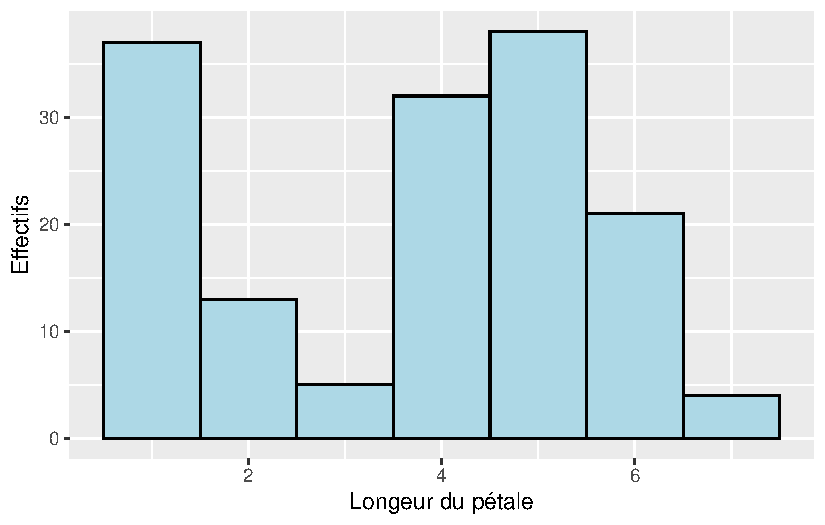
\includegraphics[keepaspectratio]{analyses/statistique-univariee_files/figure-pdf/fig-histogramme-personnalise-1.pdf}}

}

\caption{\label{fig-histogramme-personnalise}un histogramme
personnalisé}

\end{figure}%

On peut alternativement indiquer un nombre de classes avec
\texttt{bins}.

\begin{Shaded}
\begin{Highlighting}[]
\FunctionTok{ggplot}\NormalTok{(iris) }\SpecialCharTok{+}
  \FunctionTok{aes}\NormalTok{(}\AttributeTok{x =}\NormalTok{ Petal.Length) }\SpecialCharTok{+}
  \FunctionTok{geom\_histogram}\NormalTok{(}\AttributeTok{bins =} \DecValTok{10}\NormalTok{, }\AttributeTok{colour =} \StringTok{"black"}\NormalTok{)}
\end{Highlighting}
\end{Shaded}

\begin{figure}[H]

\centering{

\pandocbounded{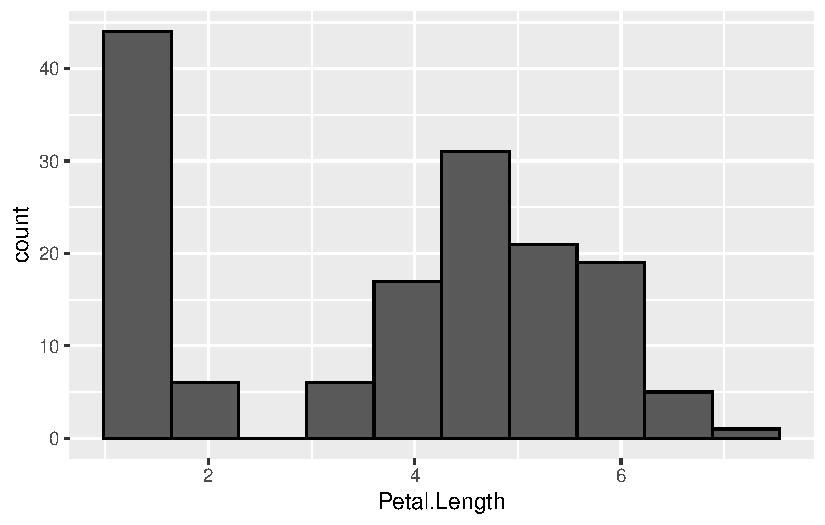
\includegraphics[keepaspectratio]{analyses/statistique-univariee_files/figure-pdf/fig-histogramme-10-classes-1.pdf}}

}

\caption{\label{fig-histogramme-10-classes}un histogramme en 10 classes}

\end{figure}%

Une représentation alternative de la distribution d'une variable peut
être obtenue avec une courbe de densité, dont la particularité est
d'avoir une surface sous la courbe égale à 1. Une telle courbe s'obtient
avec \texttt{ggplot2::geom\_density()}. Le paramètre \texttt{adjust}
permet d'ajuster le niveau de lissage de la courbe.

\begin{Shaded}
\begin{Highlighting}[]
\FunctionTok{ggplot}\NormalTok{(iris) }\SpecialCharTok{+}
  \FunctionTok{aes}\NormalTok{(}\AttributeTok{x =}\NormalTok{ Petal.Length) }\SpecialCharTok{+}
  \FunctionTok{geom\_density}\NormalTok{(}\AttributeTok{adjust =}\NormalTok{ .}\DecValTok{5}\NormalTok{)}
\end{Highlighting}
\end{Shaded}

\begin{figure}[H]

\centering{

\pandocbounded{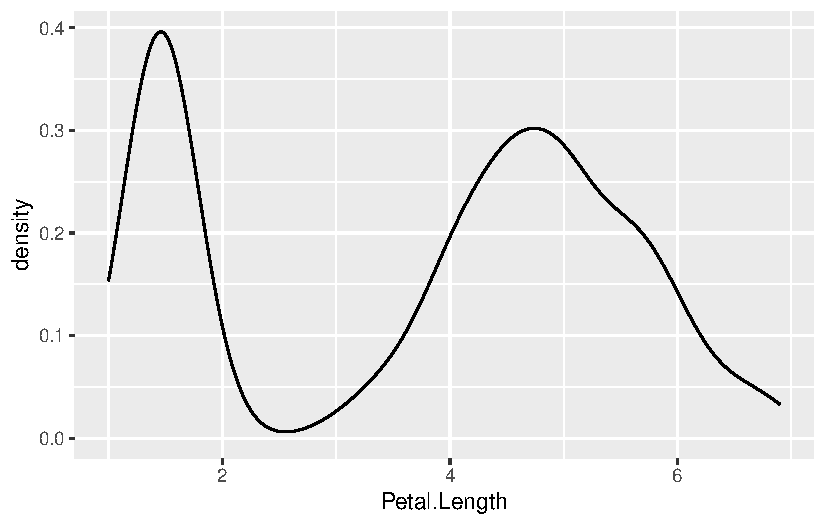
\includegraphics[keepaspectratio]{analyses/statistique-univariee_files/figure-pdf/fig-courbe-densite-1.pdf}}

}

\caption{\label{fig-courbe-densite}une courbe de densité}

\end{figure}%

\subsection{Variable catégorielle}\label{sec-graph-univ-var-cat}

Pour représenter la répartition des effectifs parmi les modalités d'une
variable catégorielle, on a souvent tendance à utiliser des diagrammes
en secteurs (camemberts). Or, ce type de représentation graphique est
très rarement appropriée~: l'œil humain préfère comparer des longueurs
plutôt que des surfaces\footnote{Voir en particulier
  \url{https://www.data-to-viz.com/caveat/pie.html} pour un exemple
  concret.}.

Dans certains contextes ou pour certaines présentations, on pourra
éventuellement considérer un diagramme en donut, mais le plus souvent,
rien ne vaut un bon vieux diagramme en barres avec
\texttt{ggplot2::geom\_bar()}. Prenons pour l'exemple la variable
\texttt{occup} du jeu de données \texttt{hdv2003} du package
\texttt{\{questionr\}}.

\begin{Shaded}
\begin{Highlighting}[]
\FunctionTok{data}\NormalTok{(}\StringTok{"hdv2003"}\NormalTok{, }\AttributeTok{package =} \StringTok{"questionr"}\NormalTok{)}
\FunctionTok{ggplot}\NormalTok{(hdv2003) }\SpecialCharTok{+}
  \FunctionTok{aes}\NormalTok{(}\AttributeTok{x =}\NormalTok{ occup) }\SpecialCharTok{+}
  \FunctionTok{geom\_bar}\NormalTok{()}
\end{Highlighting}
\end{Shaded}

\begin{figure}[H]

\centering{

\pandocbounded{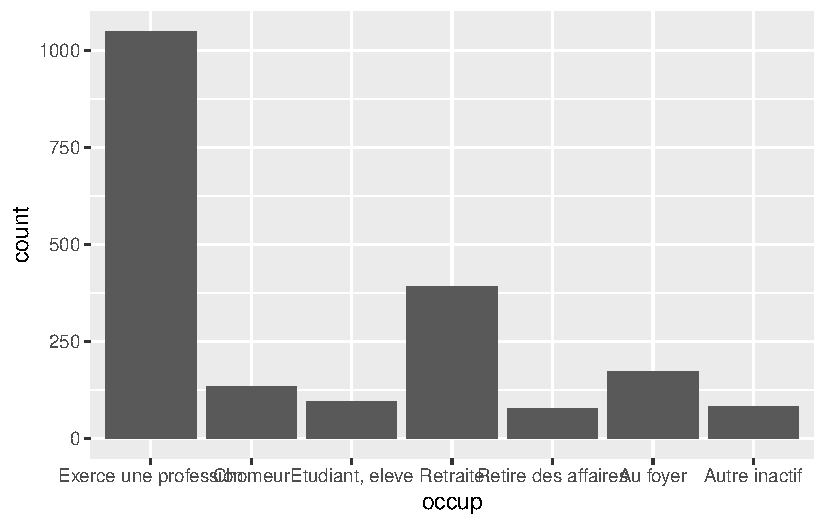
\includegraphics[keepaspectratio]{analyses/statistique-univariee_files/figure-pdf/fig-diag-barres-simple-1.pdf}}

}

\caption{\label{fig-diag-barres-simple}un diagramme en barres simple}

\end{figure}%

\begin{tcolorbox}[enhanced jigsaw, toptitle=1mm, bottomtitle=1mm, colframe=quarto-callout-tip-color-frame, toprule=.15mm, left=2mm, bottomrule=.15mm, opacitybacktitle=0.6, opacityback=0, coltitle=black, breakable, rightrule=.15mm, arc=.35mm, title=\textcolor{quarto-callout-tip-color}{\faLightbulb}\hspace{0.5em}{Astuce}, colbacktitle=quarto-callout-tip-color!10!white, titlerule=0mm, leftrule=.75mm, colback=white]

Là encore, \texttt{\{ggplot2\}} a calculé de lui-même le nombre
d'observations de chaque modalité, en utilisant cette fois la
statistique \texttt{ggplot2::stat\_count()}.

\end{tcolorbox}

Si l'on souhaite représenter des pourcentages plutôt que des effectifs,
le plus simple est d'avoir recours à la statistique
\texttt{ggstats::stat\_prop()} du package
\texttt{\{ggstats\}}\footnote{Cette statistique est également disponible
  via le package \texttt{\{GGally\}}.}. Pour appeler cette statistique,
on utilisera simplement \texttt{stat\ =\ "prop"} dans les géométries
concernées.

Cette statistique, qui sera également bien utile pour des graphiques
plus complexes, nécessite qu'on lui indique une esthétique \textbf{by}
pour dans quels sous-groupes calculés des proportions. Ici, nous avons
un seul groupe considéré et nous souhaitons des pourcentages du total.
On indiquera simplement \texttt{by\ =\ 1}.

Pour formater l'axe vertical avec des pourcentages, on pourra avoir
recours à la fonction \texttt{scales::label\_percent()} que l'on
appellera via \texttt{ggplot2::scale\_y\_continuous()}.

\begin{Shaded}
\begin{Highlighting}[]
\FunctionTok{library}\NormalTok{(ggstats)}
\FunctionTok{ggplot}\NormalTok{(hdv2003) }\SpecialCharTok{+}
  \FunctionTok{aes}\NormalTok{(}\AttributeTok{x =}\NormalTok{ occup, }\AttributeTok{y =} \FunctionTok{after\_stat}\NormalTok{(prop), }\AttributeTok{by =} \DecValTok{1}\NormalTok{) }\SpecialCharTok{+}
  \FunctionTok{geom\_bar}\NormalTok{(}\AttributeTok{stat =} \StringTok{"prop"}\NormalTok{) }\SpecialCharTok{+}
  \FunctionTok{scale\_y\_continuous}\NormalTok{(}\AttributeTok{labels =}\NormalTok{ scales}\SpecialCharTok{::}\FunctionTok{label\_percent}\NormalTok{())}
\end{Highlighting}
\end{Shaded}

\begin{figure}[H]

\centering{

\pandocbounded{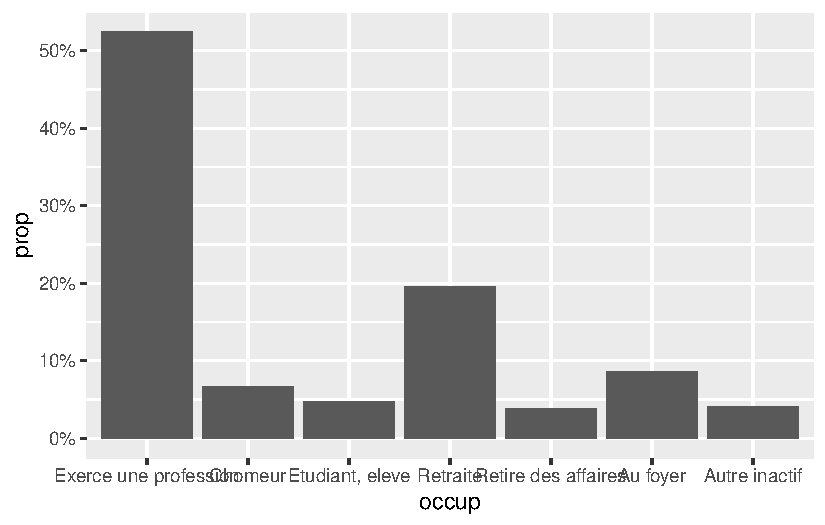
\includegraphics[keepaspectratio]{analyses/statistique-univariee_files/figure-pdf/fig-diag-barres-personnalise-1.pdf}}

}

\caption{\label{fig-diag-barres-personnalise}un diagramme en barres
épuré}

\end{figure}%

Pour une publication ou une communication, il ne faut surtout pas
hésiter à \textbf{épurer} vos graphiques (\emph{less is better!}), voire
à trier les modalités en fonction de leur fréquence pour faciliter la
lecture (ce qui se fait aisément avec \texttt{forcats::fct\_infreq()}).

\begin{Shaded}
\begin{Highlighting}[]
\FunctionTok{ggplot}\NormalTok{(hdv2003) }\SpecialCharTok{+}
  \FunctionTok{aes}\NormalTok{(}\AttributeTok{x =}\NormalTok{ forcats}\SpecialCharTok{::}\FunctionTok{fct\_infreq}\NormalTok{(occup), }
      \AttributeTok{y =} \FunctionTok{after\_stat}\NormalTok{(prop), }\AttributeTok{by =} \DecValTok{1}\NormalTok{) }\SpecialCharTok{+}
  \FunctionTok{geom\_bar}\NormalTok{(}\AttributeTok{stat =} \StringTok{"prop"}\NormalTok{, }
           \AttributeTok{fill =} \StringTok{"\#4477AA"}\NormalTok{, }\AttributeTok{colour =} \StringTok{"black"}\NormalTok{) }\SpecialCharTok{+}
  \FunctionTok{geom\_text}\NormalTok{(}
    \FunctionTok{aes}\NormalTok{(}\AttributeTok{label =} \FunctionTok{after\_stat}\NormalTok{(prop) }\SpecialCharTok{|\textgreater{}} 
\NormalTok{          scales}\SpecialCharTok{::}\FunctionTok{percent}\NormalTok{(}\AttributeTok{accuracy =}\NormalTok{ .}\DecValTok{1}\NormalTok{)),}
    \AttributeTok{stat =} \StringTok{"prop"}\NormalTok{,}
    \AttributeTok{nudge\_y =}\NormalTok{ .}\DecValTok{02}
\NormalTok{  ) }\SpecialCharTok{+}
  \FunctionTok{theme\_minimal}\NormalTok{() }\SpecialCharTok{+}
  \FunctionTok{theme}\NormalTok{(}
    \AttributeTok{panel.grid =} \FunctionTok{element\_blank}\NormalTok{(),}
    \AttributeTok{axis.text.y =} \FunctionTok{element\_blank}\NormalTok{()}
\NormalTok{  ) }\SpecialCharTok{+}
  \FunctionTok{xlab}\NormalTok{(}\ConstantTok{NULL}\NormalTok{) }\SpecialCharTok{+} \FunctionTok{ylab}\NormalTok{(}\ConstantTok{NULL}\NormalTok{) }\SpecialCharTok{+}
  \FunctionTok{ggtitle}\NormalTok{(}\StringTok{"Occupation des personnes enquêtées"}\NormalTok{)}
\end{Highlighting}
\end{Shaded}

\begin{figure}[H]

\centering{

\pandocbounded{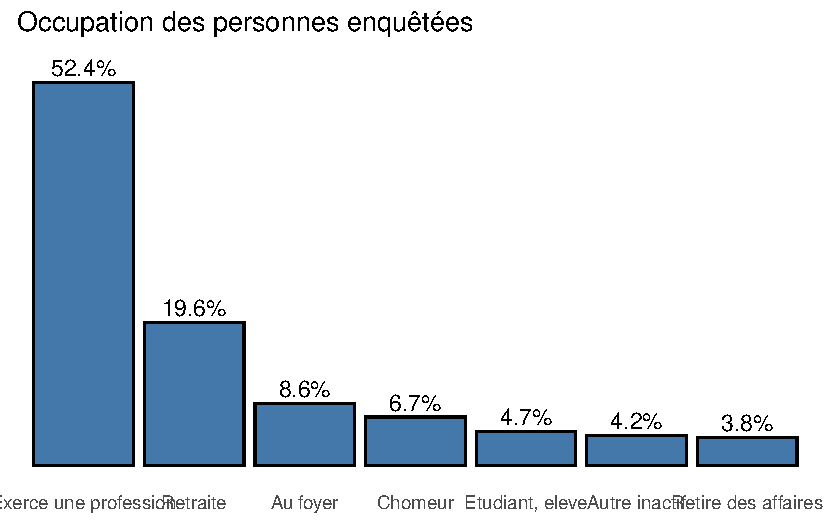
\includegraphics[keepaspectratio]{analyses/statistique-univariee_files/figure-pdf/fig-diag-barres-epure-1.pdf}}

}

\caption{\label{fig-diag-barres-epure}un diagramme en barres épuré}

\end{figure}%

Pour visualiser chaque étape du code, vous pouvez consulter le diaporama
suivant~:
\url{https://larmarange.github.io/guide-R/analyses/ressources/flipbook-geom_bar-univarie.html}

\begin{tcolorbox}[enhanced jigsaw, toptitle=1mm, bottomtitle=1mm, colframe=quarto-callout-tip-color-frame, toprule=.15mm, left=2mm, bottomrule=.15mm, opacitybacktitle=0.6, opacityback=0, coltitle=black, breakable, rightrule=.15mm, arc=.35mm, title=\textcolor{quarto-callout-tip-color}{\faLightbulb}\hspace{0.5em}{Représentation graphique de plusieurs variables catégorielles}, colbacktitle=quarto-callout-tip-color!10!white, titlerule=0mm, leftrule=.75mm, colback=white]

Pour représenter plusieurs variables catégorielles en un seul graphique,
on pourra éventuellement profiter de la géométrie
\texttt{ggalluvial::geom\_stratum()} du package \texttt{\{ggalluvial\}}.

Cette géométrie est un peu particulière. On indiquera les différentes
variables à représenter avec les esthétiques \texttt{axis1},
\texttt{axis2}, etc. On utilisera l'argument \texttt{limits} de
\texttt{ggplot2::scale\_x\_discrete()} pour personnaliser l'axe des x.

\begin{Shaded}
\begin{Highlighting}[]
\FunctionTok{library}\NormalTok{(ggalluvial)}
\FunctionTok{ggplot}\NormalTok{(hdv2003) }\SpecialCharTok{+}
  \FunctionTok{aes}\NormalTok{(}\AttributeTok{axis1 =}\NormalTok{ sexe, }\AttributeTok{axis2 =}\NormalTok{ occup, }\AttributeTok{axis3 =}\NormalTok{ sport) }\SpecialCharTok{+}
  \FunctionTok{geom\_stratum}\NormalTok{(}
    \AttributeTok{width =}\NormalTok{ .}\DecValTok{9}\NormalTok{,}
    \AttributeTok{mapping =} \FunctionTok{aes}\NormalTok{(}\AttributeTok{fill =} \FunctionTok{factor}\NormalTok{(}\FunctionTok{after\_stat}\NormalTok{(x))),}
    \AttributeTok{show.legend =} \ConstantTok{FALSE}
\NormalTok{  ) }\SpecialCharTok{+}
  \FunctionTok{geom\_text}\NormalTok{(}
    \AttributeTok{stat =} \StringTok{"stratum"}\NormalTok{, }
    \AttributeTok{mapping =} \FunctionTok{aes}\NormalTok{(}\AttributeTok{label =} \FunctionTok{after\_stat}\NormalTok{(stratum))}
\NormalTok{  ) }\SpecialCharTok{+}
  \FunctionTok{scale\_x\_discrete}\NormalTok{(}
    \AttributeTok{limits =} \FunctionTok{c}\NormalTok{(}
      \StringTok{"Sexe"}\NormalTok{,}
      \StringTok{"Occupation"}\NormalTok{,}
      \StringTok{"Pratique un sport"}
\NormalTok{    )}
\NormalTok{  ) }\SpecialCharTok{+}
\NormalTok{  khroma}\SpecialCharTok{::}\FunctionTok{scale\_fill\_bright}\NormalTok{() }\SpecialCharTok{+}
  \FunctionTok{theme\_minimal}\NormalTok{()}
\end{Highlighting}
\end{Shaded}

\pandocbounded{\includegraphics[keepaspectratio]{analyses/statistique-univariee_files/figure-pdf/unnamed-chunk-2-1.pdf}}

\end{tcolorbox}

\section{Tableaux et tris à plat}\label{sec-tri-a-plat}

Le package \texttt{\{gtsummary\}} constitue l'une des boites à outils de
l'analyste quantitativiste, car il permet de réaliser très facilement
des tableaux quasiment publiables en l'état. En matière de statistique
univariées, la fonction clé est \texttt{gtsummary::tbl\_summary()}.

Commençons avec un premier exemple rapide. On part d'un tableau de
données et on indique, avec l'argument \texttt{include}, les variables à
afficher dans le tableau statistique (si on n'indique rien, toutes les
variables du tableau de données sont considérées). Il faut noter que
l'argument \texttt{include} de \texttt{gtsummary::tbl\_summary()}
utilise la même syntaxe dite \emph{tidy select} que
\texttt{dplyr::select()} (cf. Section~\ref{sec-dplyr-select}). On peut
indiquer tout autant des variables catégorielles que des variables
continues.

\begin{Shaded}
\begin{Highlighting}[]
\FunctionTok{library}\NormalTok{(gtsummary)}
\NormalTok{hdv2003 }\SpecialCharTok{|\textgreater{}} 
  \FunctionTok{tbl\_summary}\NormalTok{(}\AttributeTok{include =} \FunctionTok{c}\NormalTok{(age, occup))}
\end{Highlighting}
\end{Shaded}

\begin{table}

\caption{\label{tbl-tableau-simple}un tableau simple}

\centering{

\fontsize{12.0pt}{14.4pt}\selectfont
\begin{tabular*}{\linewidth}{@{\extracolsep{\fill}}lc}
\toprule
\textbf{Characteristic} & \textbf{N = 2,000}\textsuperscript{\textit{1}} \\ 
\midrule\addlinespace[2.5pt]
age & 48 (35, 60) \\ 
occup &  \\ 
    Exerce une profession & 1,049 (52\%) \\ 
    Chomeur & 134 (6.7\%) \\ 
    Etudiant, eleve & 94 (4.7\%) \\ 
    Retraite & 392 (20\%) \\ 
    Retire des affaires & 77 (3.9\%) \\ 
    Au foyer & 171 (8.6\%) \\ 
    Autre inactif & 83 (4.2\%) \\ 
\bottomrule
\end{tabular*}
\begin{minipage}{\linewidth}
\textsuperscript{\textit{1}}Median (Q1, Q3); n (\%)\\
\end{minipage}

}

\end{table}%

\begin{tcolorbox}[enhanced jigsaw, toptitle=1mm, bottomtitle=1mm, colframe=quarto-callout-important-color-frame, toprule=.15mm, left=2mm, bottomrule=.15mm, opacitybacktitle=0.6, opacityback=0, coltitle=black, breakable, rightrule=.15mm, arc=.35mm, title=\textcolor{quarto-callout-important-color}{\faExclamation}\hspace{0.5em}{Remarque sur les types de variables et les sélecteurs associés}, colbacktitle=quarto-callout-important-color!10!white, titlerule=0mm, leftrule=.75mm, colback=white]

\texttt{\{gtsummary\}} permets de réaliser des tableaux statistiques
combinant plusieurs variables, l'affichage des résultats pouvant
dépendre du type de variables.

Par défaut, \texttt{\{gtsummary\}} considère qu'une variable est
\textbf{catégorielle} s'il s'agit d'un facteur, d'une variable textuelle
ou d'une variable numérique ayant moins de 10 valeurs différentes.

Une variable sera considérée comme \textbf{dichotomique} (variable
catégorielle à seulement deux modalités) s'il s'agit d'un vecteur
logique (\texttt{TRUE}/\texttt{FALSE}), d'une variable textuelle codée
\texttt{yes}/\texttt{no} ou d'une variable numérique codée
\texttt{0}/\texttt{1}.

Dans les autres cas, une variable numérique sera considérée comme
\textbf{continue}.

Si vous utilisez des vecteurs labellisés (cf.
Chapitre~\ref{sec-etiquettes-valeurs}), vous devez les convertir, en
amont, en facteurs ou en variables numériques. Voir l'extension
\texttt{\{labelled\}} et les fonctions \texttt{labelled::to\_factor()},
\texttt{labelled::unlabelled()} et \texttt{unclass()}.

Au besoin, il est possible de forcer le type d'une variable avec
l'argument \texttt{type} de \texttt{gtsummary::tbl\_summary()}.

\texttt{\{gtsummary\}} fournit des sélecteurs qui peuvent être utilisés
dans les options des différentes fonctions, en particulier
\texttt{gtsummary::all\_continuous()} pour les variables continues,
\texttt{gtsummary::all\_dichotolous()} pour les variables dichotomiques
et \texttt{gtsummary::all\_categorical()} pour les variables
catégorielles. Cela inclue les variables dichotomiques. Il faut utiliser
\texttt{all\_categorical(dichotomous\ =\ FALSE)} pour sélectionner les
variables catégorielles en excluant les variables dichotomiques.

\end{tcolorbox}

\subsection{Thème du tableau}\label{sec-theme-gtsummary}

\texttt{\{gtsummary\}} fournit plusieurs fonctions préfixées
\texttt{theme\_gtsummary\_*()} permettant de modifier l'affichage par
défaut des tableaux. Vous aurez notez que, par défaut,
\texttt{\{gtsummary\}} est anglophone.

La fonction \texttt{gtsummary::theme\_gtsummary\_journal()} permets
d'adopter les standards de certaines grandes revues scientifiques telles
que \emph{JAMA} (\emph{Journal of the American Medical Association}),
\emph{The Lancet} ou encore le \emph{NEJM} (\emph{New England Journal of
Medicine}).

La fonction \texttt{gtsummary::theme\_gtsummary\_language()} permet de
modifier la langue utilisée par défaut dans les tableaux. Les options
\texttt{decimal.mark} et \texttt{big.mark} permettent de définir
respectivement le séparateur de décimales et le séparateur des milliers.
Ainsi, pour présenter un tableau en français, on appliquera en début de
script~:

\begin{Shaded}
\begin{Highlighting}[]
\FunctionTok{theme\_gtsummary\_language}\NormalTok{(}
  \AttributeTok{language =} \StringTok{"fr"}\NormalTok{, }
  \AttributeTok{decimal.mark =} \StringTok{","}\NormalTok{, }
  \AttributeTok{big.mark =} \StringTok{" "}
\NormalTok{)}
\end{Highlighting}
\end{Shaded}

\begin{verbatim}
Setting theme "language: fr"
\end{verbatim}

Ce thème sera appliqué à tous les tableaux ultérieurs.

\begin{Shaded}
\begin{Highlighting}[]
\NormalTok{hdv2003 }\SpecialCharTok{|\textgreater{}} 
  \FunctionTok{tbl\_summary}\NormalTok{(}\AttributeTok{include =} \FunctionTok{c}\NormalTok{(age, occup))}
\end{Highlighting}
\end{Shaded}

\begin{table}

\caption{\label{tbl-tableau-simple-fr}un tableau simple en français}

\centering{

\fontsize{12.0pt}{14.4pt}\selectfont
\begin{tabular*}{\linewidth}{@{\extracolsep{\fill}}lc}
\toprule
\textbf{Caractéristique} & \textbf{N = 2 000}\textsuperscript{\textit{1}} \\ 
\midrule\addlinespace[2.5pt]
age & 48 (35 – 60) \\ 
occup &  \\ 
    Exerce une profession & 1 049 (52\%) \\ 
    Chomeur & 134 (6,7\%) \\ 
    Etudiant, eleve & 94 (4,7\%) \\ 
    Retraite & 392 (20\%) \\ 
    Retire des affaires & 77 (3,9\%) \\ 
    Au foyer & 171 (8,6\%) \\ 
    Autre inactif & 83 (4,2\%) \\ 
\bottomrule
\end{tabular*}
\begin{minipage}{\linewidth}
\textsuperscript{\textit{1}}Médiane (Q1 -- Q3); n (\%)\\
\end{minipage}

}

\end{table}%

\subsection{Étiquettes des variables}\label{uxe9tiquettes-des-variables}

\texttt{gtsummary}, par défaut, prends en compte les étiquettes de
variables (cf. Chapitre~\ref{sec-etiquettes-variables}), si elles
existent, et sinon utilisera le nom de chaque variable dans le tableau.
Pour rappel, les étiquettes de variables peuvent être manipulées avec
l'extension \texttt{\{labelled\}} et les fonctions
\texttt{labelled::var\_label()} et
\texttt{labelled::set\_variable\_labels()}.

Il est aussi possible d'utiliser l'option \texttt{label} de
\texttt{gtsummary::tbl\_summary()} pour indiquer des étiquettes
personnalisées.

\begin{Shaded}
\begin{Highlighting}[]
\NormalTok{hdv2003 }\SpecialCharTok{|\textgreater{}} 
\NormalTok{  labelled}\SpecialCharTok{::}\FunctionTok{set\_variable\_labels}\NormalTok{(}
    \AttributeTok{occup =} \StringTok{"Occupation actuelle"}
\NormalTok{  ) }\SpecialCharTok{|\textgreater{}} 
  \FunctionTok{tbl\_summary}\NormalTok{(}
    \AttributeTok{include =} \FunctionTok{c}\NormalTok{(age, occup, heures.tv),}
    \AttributeTok{label =} \FunctionTok{list}\NormalTok{(age }\SpecialCharTok{\textasciitilde{}} \StringTok{"Âge médian"}\NormalTok{)}
\NormalTok{  )}
\end{Highlighting}
\end{Shaded}

\begin{table}

\caption{\label{tbl-tableau-etiquette}un tableau étiquetté}

\centering{

\fontsize{12.0pt}{14.4pt}\selectfont
\begin{tabular*}{\linewidth}{@{\extracolsep{\fill}}lc}
\toprule
\textbf{Caractéristique} & \textbf{N = 2 000}\textsuperscript{\textit{1}} \\ 
\midrule\addlinespace[2.5pt]
Âge médian & 48 (35 – 60) \\ 
Occupation actuelle &  \\ 
    Exerce une profession & 1 049 (52\%) \\ 
    Chomeur & 134 (6,7\%) \\ 
    Etudiant, eleve & 94 (4,7\%) \\ 
    Retraite & 392 (20\%) \\ 
    Retire des affaires & 77 (3,9\%) \\ 
    Au foyer & 171 (8,6\%) \\ 
    Autre inactif & 83 (4,2\%) \\ 
heures.tv & 2,00 (1,00 – 3,00) \\ 
    Manquant & 5 \\ 
\bottomrule
\end{tabular*}
\begin{minipage}{\linewidth}
\textsuperscript{\textit{1}}Médiane (Q1 -- Q3); n (\%)\\
\end{minipage}

}

\end{table}%

Pour modifier les modalités d'une variable catégorielle, il faut
modifier en amont les niveaux du facteur correspondant.

\begin{tcolorbox}[enhanced jigsaw, toptitle=1mm, bottomtitle=1mm, colframe=quarto-callout-important-color-frame, toprule=.15mm, left=2mm, bottomrule=.15mm, opacitybacktitle=0.6, opacityback=0, coltitle=black, breakable, rightrule=.15mm, arc=.35mm, title=\textcolor{quarto-callout-important-color}{\faExclamation}\hspace{0.5em}{Remarque sur la syntaxe des options}, colbacktitle=quarto-callout-important-color!10!white, titlerule=0mm, leftrule=.75mm, colback=white]

De nombreuses options des fonctions de \texttt{\{gtsummary\}} peuvent
s'appliquer seulement à une ou certaines variables. Pour ces options-là,
\texttt{\{gtsummary\}} attends une formule de la forme
\texttt{variables\ concernées\ \textasciitilde{}\ valeur\ de\ l\textquotesingle{}option}
ou bien une liste de formules ayant cette forme.

Par exemple, pour modifier l'étiquette associée à une certaine variable,
on peut utiliser l'option \texttt{label} de
\texttt{gtsummary::tbl\_summary()}.

\begin{Shaded}
\begin{Highlighting}[]
\NormalTok{trial }\SpecialCharTok{|\textgreater{}} 
  \FunctionTok{tbl\_summary}\NormalTok{(}\AttributeTok{label =}\NormalTok{ age }\SpecialCharTok{\textasciitilde{}} \StringTok{"Âge"}\NormalTok{)}
\end{Highlighting}
\end{Shaded}

Lorsque l'on souhaite passer plusieurs options pour plusieurs variables
différentes, on utilisera une \texttt{list()}.

\begin{Shaded}
\begin{Highlighting}[]
\NormalTok{trial }\SpecialCharTok{|\textgreater{}} 
  \FunctionTok{tbl\_summary}\NormalTok{(}\AttributeTok{label =} \FunctionTok{list}\NormalTok{(age }\SpecialCharTok{\textasciitilde{}} \StringTok{"Âge"}\NormalTok{, trt }\SpecialCharTok{\textasciitilde{}} \StringTok{"Traitement"}\NormalTok{))}
\end{Highlighting}
\end{Shaded}

\texttt{\{gtsummary\}} est très flexible sur la manière d'indiquer la ou
les variables concernées. Il peut s'agir du nom de la variable, d'une
chaîne de caractères contenant le nom de la variable, ou d'un vecteur
contenant le nom de la variable. Les syntaxes ci-dessous sont ainsi
équivalentes.

\begin{Shaded}
\begin{Highlighting}[]
\NormalTok{trial }\SpecialCharTok{|\textgreater{}} 
  \FunctionTok{tbl\_summary}\NormalTok{(}\AttributeTok{label =}\NormalTok{ age }\SpecialCharTok{\textasciitilde{}} \StringTok{"Âge"}\NormalTok{)}
\NormalTok{trial }\SpecialCharTok{|\textgreater{}} 
  \FunctionTok{tbl\_summary}\NormalTok{(}\AttributeTok{label =} \StringTok{"age"} \SpecialCharTok{\textasciitilde{}} \StringTok{"Âge"}\NormalTok{)}
\NormalTok{v }\OtherTok{\textless{}{-}} \StringTok{"age"}
\NormalTok{trial }\SpecialCharTok{|\textgreater{}} 
  \FunctionTok{tbl\_summary}\NormalTok{(}\AttributeTok{label =}\NormalTok{ v }\SpecialCharTok{\textasciitilde{}} \StringTok{"Âge"}\NormalTok{)}
\end{Highlighting}
\end{Shaded}

Pour appliquer le même changement à plusieurs variables, plusieurs
syntaxes sont acceptées pour lister plusieurs variables.

\begin{Shaded}
\begin{Highlighting}[]
\NormalTok{trial }\SpecialCharTok{|\textgreater{}} 
  \FunctionTok{tbl\_summary}\NormalTok{(}\AttributeTok{label =} \FunctionTok{c}\NormalTok{(}\StringTok{"age"}\NormalTok{, }\StringTok{"trt"}\NormalTok{) }\SpecialCharTok{\textasciitilde{}} \StringTok{"Une même étiquette"}\NormalTok{)}
\NormalTok{trial }\SpecialCharTok{|\textgreater{}} 
  \FunctionTok{tbl\_summary}\NormalTok{(}\AttributeTok{label =} \FunctionTok{c}\NormalTok{(age, trt) }\SpecialCharTok{\textasciitilde{}} \StringTok{"Une même étiquette"}\NormalTok{)}
\end{Highlighting}
\end{Shaded}

Il est également possible d'utiliser la syntaxe \texttt{\{tidyselect\}}
et les sélecteurs de \texttt{\{tidyselect\}} comme
\texttt{tidyselect::everything()}, \texttt{tidyselect::starts\_with()},
\texttt{tidyselect::contains()} ou \texttt{tidyselect::all\_of()}. Ces
différents sélecteurs peuvent être combinés au sein d'un \texttt{c()}.

\begin{Shaded}
\begin{Highlighting}[]
\NormalTok{trial }\SpecialCharTok{|\textgreater{}} 
  \FunctionTok{tbl\_summary}\NormalTok{(}
    \AttributeTok{label =} \FunctionTok{everything}\NormalTok{() }\SpecialCharTok{\textasciitilde{}} \StringTok{"Une même étiquette"}
\NormalTok{  )}
\NormalTok{trial }\SpecialCharTok{|\textgreater{}} 
  \FunctionTok{tbl\_summary}\NormalTok{(}
    \AttributeTok{label =} \FunctionTok{starts\_with}\NormalTok{(}\StringTok{"a"}\NormalTok{) }\SpecialCharTok{\textasciitilde{}} \StringTok{"Une même étiquette"}
\NormalTok{  )}
\NormalTok{trial }\SpecialCharTok{|\textgreater{}} 
  \FunctionTok{tbl\_summary}\NormalTok{(}
    \AttributeTok{label =} \FunctionTok{c}\NormalTok{(}\FunctionTok{everything}\NormalTok{(), }\SpecialCharTok{{-}}\NormalTok{age, }\SpecialCharTok{{-}}\NormalTok{trt) }\SpecialCharTok{\textasciitilde{}} \StringTok{"Une même étiquette"}
\NormalTok{  )}
\NormalTok{trial }\SpecialCharTok{|\textgreater{}} 
  \FunctionTok{tbl\_summary}\NormalTok{(}
    \AttributeTok{label =}\NormalTok{ age}\SpecialCharTok{:}\NormalTok{trt }\SpecialCharTok{\textasciitilde{}} \StringTok{"Une même étiquette"}
\NormalTok{  )}
\end{Highlighting}
\end{Shaded}

Bien sûr, il est possible d'utiliser les sélecteurs propres à
\texttt{\{gtsummary\}}.

\begin{Shaded}
\begin{Highlighting}[]
\NormalTok{trial }\SpecialCharTok{|\textgreater{}} 
  \FunctionTok{tbl\_summary}\NormalTok{(}
    \AttributeTok{label =} \FunctionTok{all\_continuous}\NormalTok{() }\SpecialCharTok{\textasciitilde{}} \StringTok{"Une même étiquette"}
\NormalTok{  )}
\NormalTok{trial }\SpecialCharTok{|\textgreater{}} 
  \FunctionTok{tbl\_summary}\NormalTok{(}
    \AttributeTok{label =} \FunctionTok{list}\NormalTok{(}
      \FunctionTok{all\_continuous}\NormalTok{() }\SpecialCharTok{\textasciitilde{}} \StringTok{"Variable continue"}\NormalTok{,}
      \FunctionTok{all\_dichotomous}\NormalTok{() }\SpecialCharTok{\textasciitilde{}} \StringTok{"Variable dichotomique"}\NormalTok{,}
      \FunctionTok{all\_categorical}\NormalTok{(}\AttributeTok{dichotomous =} \ConstantTok{FALSE}\NormalTok{) }\SpecialCharTok{\textasciitilde{}} \StringTok{"Variable catégorielle"}
\NormalTok{    )}
\NormalTok{  )}
\end{Highlighting}
\end{Shaded}

Enfin, si l'on ne précise rien à gauche du \texttt{\textasciitilde{}},
ce sera considéré comme équivalent à \texttt{everything()}. Les deux
syntaxes ci-dessous sont donc équivalentes.

\begin{Shaded}
\begin{Highlighting}[]
\NormalTok{trial }\SpecialCharTok{|\textgreater{}} 
  \FunctionTok{tbl\_summary}\NormalTok{(}\AttributeTok{label =} \SpecialCharTok{\textasciitilde{}} \StringTok{"Une même étiquette"}\NormalTok{)}
\NormalTok{trial }\SpecialCharTok{|\textgreater{}} 
  \FunctionTok{tbl\_summary}\NormalTok{(}
    \AttributeTok{label =} \FunctionTok{everything}\NormalTok{() }\SpecialCharTok{\textasciitilde{}} \StringTok{"Une même étiquette"}
\NormalTok{  )}
\end{Highlighting}
\end{Shaded}

\end{tcolorbox}

\subsection{Statistiques affichées}\label{statistiques-affichuxe9es}

Le paramètre \texttt{statistic} permets de sélectionner les statistiques
à afficher pour chaque variable. On indiquera une chaîne de caractères
dont les différentes statistiques seront indiquées entre accolades
(\texttt{\{\}}).

Pour une \textbf{variable continue}, on pourra utiliser
\texttt{\{median\}} pour la médiane, \texttt{\{mean\}} pour la moyenne,
\texttt{\{sd\}} pour l'écart type, \texttt{\{var\}} pour la variance,
\texttt{\{min\}} pour le minimum, \texttt{\{max\}} pour le maximum, ou
encore \texttt{\{p\#\#\}} (en remplaçant \texttt{\#\#} par un nombre
entier entre 00 et 100) pour le percentile correspondant (par exemple
\texttt{p25} et \texttt{p75} pour le premier et le troisième quartile).
Utilisez \texttt{gtsummary::all\_continous()} pour sélectionner toutes
les variables continues.

\begin{Shaded}
\begin{Highlighting}[]
\NormalTok{hdv2003 }\SpecialCharTok{|\textgreater{}}
  \FunctionTok{tbl\_summary}\NormalTok{(}
    \AttributeTok{include =} \FunctionTok{c}\NormalTok{(age, heures.tv),}
    \AttributeTok{statistic =} 
      \FunctionTok{all\_continuous}\NormalTok{() }\SpecialCharTok{\textasciitilde{}} \StringTok{"Moy. : \{mean\} [min{-}max : \{min\} {-} \{max\}]"}
\NormalTok{  )}
\end{Highlighting}
\end{Shaded}

\begin{table}

\caption{\label{tbl-stat-var-cont}statistiques personnalisées pour une
variable continue}

\centering{

\fontsize{12.0pt}{14.4pt}\selectfont
\begin{tabular*}{\linewidth}{@{\extracolsep{\fill}}lc}
\toprule
\textbf{Caractéristique} & \textbf{N = 2 000}\textsuperscript{\textit{1}} \\ 
\midrule\addlinespace[2.5pt]
age & Moy. : 48 [min-max : 18 - 97] \\ 
heures.tv & Moy. : 2,25 [min-max : 0,00 - 12,00] \\ 
    Manquant & 5 \\ 
\bottomrule
\end{tabular*}
\begin{minipage}{\linewidth}
\textsuperscript{\textit{1}}Moy. : Moyenne {[}min-max : Min - Max{]}\\
\end{minipage}

}

\end{table}%

Il est possible d'afficher des statistiques différentes pour chaque
variable.

\begin{Shaded}
\begin{Highlighting}[]
\NormalTok{hdv2003 }\SpecialCharTok{|\textgreater{}}
  \FunctionTok{tbl\_summary}\NormalTok{(}
    \AttributeTok{include =} \FunctionTok{c}\NormalTok{(age, heures.tv),}
    \AttributeTok{statistic =} \FunctionTok{list}\NormalTok{(}
\NormalTok{      age }\SpecialCharTok{\textasciitilde{}} \StringTok{"Méd. : \{median\} [\{p25\} {-} \{p75\}]"}\NormalTok{,}
\NormalTok{      heures.tv }\SpecialCharTok{\textasciitilde{}} \StringTok{"Moy. : \{mean\} (\{sd\})"}
\NormalTok{    )}
\NormalTok{  )}
\end{Highlighting}
\end{Shaded}

\begin{table}

\caption{\label{tbl-stat-var-cont2}statistiques personnalisées pour une
variable continue (2)}

\centering{

\fontsize{12.0pt}{14.4pt}\selectfont
\begin{tabular*}{\linewidth}{@{\extracolsep{\fill}}lc}
\toprule
\textbf{Caractéristique} & \textbf{N = 2 000}\textsuperscript{\textit{1}} \\ 
\midrule\addlinespace[2.5pt]
age & Méd. : 48 [35 - 60] \\ 
heures.tv & Moy. : 2,25 (1,78) \\ 
    Manquant & 5 \\ 
\bottomrule
\end{tabular*}
\begin{minipage}{\linewidth}
\textsuperscript{\textit{1}}Méd. : Médiane {[}Q1 - Q3{]}; Moy. : Moyenne (ET)\\
\end{minipage}

}

\end{table}%

Pour les variables continues, il est également possible d'indiquer le
nom d'une fonction personnalisée qui prends un vecteur et renvoie une
valeur résumée. Par exemple, pour afficher la moyenne des carrés~:

\begin{Shaded}
\begin{Highlighting}[]
\NormalTok{moy\_carres }\OtherTok{\textless{}{-}} \ControlFlowTok{function}\NormalTok{(x) \{}
  \FunctionTok{mean}\NormalTok{(x}\SpecialCharTok{\^{}}\DecValTok{2}\NormalTok{, }\AttributeTok{na.rm =} \ConstantTok{TRUE}\NormalTok{)}
\NormalTok{\}}
\NormalTok{hdv2003 }\SpecialCharTok{|\textgreater{}}
  \FunctionTok{tbl\_summary}\NormalTok{(}
    \AttributeTok{include =}\NormalTok{ heures.tv,}
    \AttributeTok{statistic =} \SpecialCharTok{\textasciitilde{}} \StringTok{"MC : \{moy\_carres\}"}
\NormalTok{  )}
\end{Highlighting}
\end{Shaded}

\begin{table}

\caption{\label{tbl-stat-var-cont3}statiques personnalisées pour une
variable continue (3)}

\centering{

\fontsize{12.0pt}{14.4pt}\selectfont
\begin{tabular*}{\linewidth}{@{\extracolsep{\fill}}lc}
\toprule
\textbf{Caractéristique} & \textbf{N = 2 000}\textsuperscript{\textit{1}} \\ 
\midrule\addlinespace[2.5pt]
heures.tv & MC : 8,20 \\ 
    Manquant & 5 \\ 
\bottomrule
\end{tabular*}
\begin{minipage}{\linewidth}
\textsuperscript{\textit{1}}MC : moy\_carres\\
\end{minipage}

}

\end{table}%

Pour une \textbf{variable catégorielle}, les statistiques possibles sont
\texttt{\{n\}} le nombre d'observations, \texttt{\{N\}} le nombre total
d'observations, et \texttt{\{p\}} le pourcentage correspondant. Utilisez
\texttt{gtsummary::all\_categorical()} pour sélectionner toutes les
variables catégorielles.

\begin{Shaded}
\begin{Highlighting}[]
\NormalTok{hdv2003 }\SpecialCharTok{|\textgreater{}}
  \FunctionTok{tbl\_summary}\NormalTok{(}
    \AttributeTok{include =}\NormalTok{ occup,}
    \AttributeTok{statistic =} \FunctionTok{all\_categorical}\NormalTok{() }\SpecialCharTok{\textasciitilde{}} \StringTok{"\{p\} \% (\{n\}/\{N\})"}
\NormalTok{  )}
\end{Highlighting}
\end{Shaded}

\begin{table}

\caption{\label{tbl-stat-var-cat}statiques personnalisées pour une
variable catégorielle}

\centering{

\fontsize{12.0pt}{14.4pt}\selectfont
\begin{tabular*}{\linewidth}{@{\extracolsep{\fill}}lc}
\toprule
\textbf{Caractéristique} & \textbf{N = 2 000}\textsuperscript{\textit{1}} \\ 
\midrule\addlinespace[2.5pt]
occup &  \\ 
    Exerce une profession & 52 \% (1 049/2 000) \\ 
    Chomeur & 6,7 \% (134/2 000) \\ 
    Etudiant, eleve & 4,7 \% (94/2 000) \\ 
    Retraite & 20 \% (392/2 000) \\ 
    Retire des affaires & 3,9 \% (77/2 000) \\ 
    Au foyer & 8,6 \% (171/2 000) \\ 
    Autre inactif & 4,2 \% (83/2 000) \\ 
\bottomrule
\end{tabular*}
\begin{minipage}{\linewidth}
\textsuperscript{\textit{1}}\% \% (n/N)\\
\end{minipage}

}

\end{table}%

Il est possible, pour une variable catégorielle, de trier les modalités
de la plus fréquente à la moins fréquente avec le paramètre
\texttt{sort}.

\begin{Shaded}
\begin{Highlighting}[]
\NormalTok{hdv2003 }\SpecialCharTok{|\textgreater{}}
  \FunctionTok{tbl\_summary}\NormalTok{(}
    \AttributeTok{include =}\NormalTok{ occup,}
    \AttributeTok{sort =} \FunctionTok{all\_categorical}\NormalTok{() }\SpecialCharTok{\textasciitilde{}} \StringTok{"frequency"}
\NormalTok{  )}
\end{Highlighting}
\end{Shaded}

\begin{table}

\caption{\label{tbl-stat-var-cat-sort}variable catégorielle triée par
fréquence}

\centering{

\fontsize{12.0pt}{14.4pt}\selectfont
\begin{tabular*}{\linewidth}{@{\extracolsep{\fill}}lc}
\toprule
\textbf{Caractéristique} & \textbf{N = 2 000}\textsuperscript{\textit{1}} \\ 
\midrule\addlinespace[2.5pt]
occup &  \\ 
    Exerce une profession & 1 049 (52\%) \\ 
    Retraite & 392 (20\%) \\ 
    Au foyer & 171 (8,6\%) \\ 
    Chomeur & 134 (6,7\%) \\ 
    Etudiant, eleve & 94 (4,7\%) \\ 
    Autre inactif & 83 (4,2\%) \\ 
    Retire des affaires & 77 (3,9\%) \\ 
\bottomrule
\end{tabular*}
\begin{minipage}{\linewidth}
\textsuperscript{\textit{1}}n (\%)\\
\end{minipage}

}

\end{table}%

Pour toutes les variables (catégorielles et continues), les statistiques
suivantes sont également disponibles~:

\begin{itemize}
\tightlist
\item
  \texttt{\{N\_obs\}} le nombre total d'observations,
\item
  \texttt{\{N\_miss\}} le nombre d'observations manquantes
  (\texttt{NA}),
\item
  \texttt{\{N\_nonmiss\}} le nombre d'observations non manquantes,
\item
  \texttt{\{p\_miss\}} le pourcentage d'observations manquantes
  (i.e.~\texttt{N\_miss\ /\ N\_obs}) et
\item
  \texttt{\{p\_nonmiss\}} le pourcentage d'observations non manquantes
  (i.e.~\texttt{N\_nonmiss\ /\ N\_obs}).
\end{itemize}

\subsection{Affichage du nom des
statistiques}\label{affichage-du-nom-des-statistiques}

Lorsque l'on affiche de multiples statistiques, la liste des
statistiques est regroupée dans une note de tableau qui peut vite
devenir un peu confuse.

\begin{Shaded}
\begin{Highlighting}[]
\NormalTok{tbl }\OtherTok{\textless{}{-}}\NormalTok{ hdv2003 }\SpecialCharTok{|\textgreater{}}
  \FunctionTok{tbl\_summary}\NormalTok{(}
    \AttributeTok{include =} \FunctionTok{c}\NormalTok{(age, heures.tv, occup),}
    \AttributeTok{statistic =} \FunctionTok{list}\NormalTok{(}
\NormalTok{      age }\SpecialCharTok{\textasciitilde{}} \StringTok{"\{mean\} (\{sd\})"}\NormalTok{,}
\NormalTok{      heures.tv }\SpecialCharTok{\textasciitilde{}} \StringTok{"\{median\} [\{p25\} {-} \{p75\}]"}
\NormalTok{    )}
\NormalTok{  )}
\NormalTok{tbl}
\end{Highlighting}
\end{Shaded}

\begin{table}

\caption{\label{tbl-stat-nom}tableau par défaut}

\centering{

\fontsize{12.0pt}{14.4pt}\selectfont
\begin{tabular*}{\linewidth}{@{\extracolsep{\fill}}lc}
\toprule
\textbf{Caractéristique} & \textbf{N = 2 000}\textsuperscript{\textit{1}} \\ 
\midrule\addlinespace[2.5pt]
age & 48 (17) \\ 
heures.tv & 2,00 [1,00 - 3,00] \\ 
    Manquant & 5 \\ 
occup &  \\ 
    Exerce une profession & 1 049 (52\%) \\ 
    Chomeur & 134 (6,7\%) \\ 
    Etudiant, eleve & 94 (4,7\%) \\ 
    Retraite & 392 (20\%) \\ 
    Retire des affaires & 77 (3,9\%) \\ 
    Au foyer & 171 (8,6\%) \\ 
    Autre inactif & 83 (4,2\%) \\ 
\bottomrule
\end{tabular*}
\begin{minipage}{\linewidth}
\textsuperscript{\textit{1}}Moyenne (ET); Médiane {[}Q1 - Q3{]}; n (\%)\\
\end{minipage}

}

\end{table}%

La fonction \texttt{gtsummary::add\_stat\_label()} permets d'indiquer le
type de statistique à côté du nom des variables ou bien dans une colonne
dédiée, plutôt qu'en note de tableau.

\begin{Shaded}
\begin{Highlighting}[]
\NormalTok{tbl }\SpecialCharTok{|\textgreater{}} 
  \FunctionTok{add\_stat\_label}\NormalTok{()}
\end{Highlighting}
\end{Shaded}

\begin{table}

\caption{\label{tbl-stat-nom-2}ajout du nom des statistiques}

\centering{

\fontsize{12.0pt}{14.4pt}\selectfont
\begin{tabular*}{\linewidth}{@{\extracolsep{\fill}}lc}
\toprule
\textbf{Caractéristique} & \textbf{N = 2 000} \\ 
\midrule\addlinespace[2.5pt]
age, Moyenne (ET) & 48 (17) \\ 
heures.tv, Médiane [Q1 - Q3] & 2,00 [1,00 - 3,00] \\ 
    Manquant & 5 \\ 
occup, n (\%) &  \\ 
    Exerce une profession & 1 049 (52\%) \\ 
    Chomeur & 134 (6,7\%) \\ 
    Etudiant, eleve & 94 (4,7\%) \\ 
    Retraite & 392 (20\%) \\ 
    Retire des affaires & 77 (3,9\%) \\ 
    Au foyer & 171 (8,6\%) \\ 
    Autre inactif & 83 (4,2\%) \\ 
\bottomrule
\end{tabular*}

}

\end{table}%

\begin{Shaded}
\begin{Highlighting}[]
\NormalTok{tbl }\SpecialCharTok{|\textgreater{}} 
  \FunctionTok{add\_stat\_label}\NormalTok{(}\AttributeTok{location =} \StringTok{"column"}\NormalTok{)}
\end{Highlighting}
\end{Shaded}

\begin{table}

\caption{\label{tbl-stat-nom-3}ajout du nom des statistiques dans une
colonne séparée}

\centering{

\fontsize{12.0pt}{14.4pt}\selectfont
\begin{tabular*}{\linewidth}{@{\extracolsep{\fill}}lcc}
\toprule
\textbf{Caractéristique} & \textbf{Statistique} & \textbf{N = 2 000} \\ 
\midrule\addlinespace[2.5pt]
age & Moyenne (ET) & 48 (17) \\ 
heures.tv & Médiane [Q1 - Q3] & 2,00 [1,00 - 3,00] \\ 
    Manquant & n & 5 \\ 
occup &  &  \\ 
    Exerce une profession & n (\%) & 1 049 (52\%) \\ 
    Chomeur & n (\%) & 134 (6,7\%) \\ 
    Etudiant, eleve & n (\%) & 94 (4,7\%) \\ 
    Retraite & n (\%) & 392 (20\%) \\ 
    Retire des affaires & n (\%) & 77 (3,9\%) \\ 
    Au foyer & n (\%) & 171 (8,6\%) \\ 
    Autre inactif & n (\%) & 83 (4,2\%) \\ 
\bottomrule
\end{tabular*}

}

\end{table}%

\subsection{Forcer le type de
variable}\label{forcer-le-type-de-variable}

Comme évoqué plus haut, \texttt{\{gtsummary\}} détermine automatiquement
le type de chaque variable. Par défaut, la variable \texttt{age} du
tableau de données \texttt{trial} est traitée comme variable continue,
\texttt{death} comme dichotomique (seule la valeur 1 est affichée) et
\texttt{grade} comme variable catégorielle.

\begin{Shaded}
\begin{Highlighting}[]
\NormalTok{trial }\SpecialCharTok{|\textgreater{}}
  \FunctionTok{tbl\_summary}\NormalTok{(}
    \AttributeTok{include =} \FunctionTok{c}\NormalTok{(grade, age, death)}
\NormalTok{  )}
\end{Highlighting}
\end{Shaded}

\begin{table}

\caption{\label{tbl-types-defaut}types de variable par défaut}

\centering{

\fontsize{12.0pt}{14.4pt}\selectfont
\begin{tabular*}{\linewidth}{@{\extracolsep{\fill}}lc}
\toprule
\textbf{Caractéristique} & \textbf{N = 200}\textsuperscript{\textit{1}} \\ 
\midrule\addlinespace[2.5pt]
Grade &  \\ 
    I & 68 (34\%) \\ 
    II & 68 (34\%) \\ 
    III & 64 (32\%) \\ 
Age & 47 (38 – 57) \\ 
    Manquant & 11 \\ 
Patient Died & 112 (56\%) \\ 
\bottomrule
\end{tabular*}
\begin{minipage}{\linewidth}
\textsuperscript{\textit{1}}n (\%); Médiane (Q1 -- Q3)\\
\end{minipage}

}

\end{table}%

Il est cependant possible de forcer un certain type avec l'argument
\texttt{type}. Précision~: lorsque l'on force une variable en
dichotomique, il faut indiquer avec \texttt{value} la valeur à afficher
(les autres sont alors masquées).

\begin{Shaded}
\begin{Highlighting}[]
\NormalTok{trial }\SpecialCharTok{|\textgreater{}}
  \FunctionTok{tbl\_summary}\NormalTok{(}
    \AttributeTok{include =} \FunctionTok{c}\NormalTok{(grade, death),}
    \AttributeTok{type =} \FunctionTok{list}\NormalTok{(}
\NormalTok{      grade }\SpecialCharTok{\textasciitilde{}} \StringTok{"dichotomous"}\NormalTok{,}
\NormalTok{      death }\SpecialCharTok{\textasciitilde{}} \StringTok{"categorical"}
\NormalTok{    ),}
    \AttributeTok{value =}\NormalTok{ grade }\SpecialCharTok{\textasciitilde{}} \StringTok{"III"}\NormalTok{,}
    \AttributeTok{label =}\NormalTok{ grade }\SpecialCharTok{\textasciitilde{}} \StringTok{"Grade III"}
\NormalTok{  )}
\end{Highlighting}
\end{Shaded}

\begin{table}

\caption{\label{tbl-types-personnalises}types de variable personnalisés}

\centering{

\fontsize{12.0pt}{14.4pt}\selectfont
\begin{tabular*}{\linewidth}{@{\extracolsep{\fill}}lc}
\toprule
\textbf{Caractéristique} & \textbf{N = 200}\textsuperscript{\textit{1}} \\ 
\midrule\addlinespace[2.5pt]
Grade III & 64 (32\%) \\ 
Patient Died &  \\ 
    0 & 88 (44\%) \\ 
    1 & 112 (56\%) \\ 
\bottomrule
\end{tabular*}
\begin{minipage}{\linewidth}
\textsuperscript{\textit{1}}n (\%)\\
\end{minipage}

}

\end{table}%

Il ne faut pas oublier que, par défaut, \texttt{\{gtsummary\}} traite
les variables quantitatives avec moins de 10 valeurs comme des variables
catégorielles. Prenons un exemple~:

\begin{Shaded}
\begin{Highlighting}[]
\NormalTok{trial}\SpecialCharTok{$}\NormalTok{alea }\OtherTok{\textless{}{-}} \FunctionTok{sample}\NormalTok{(}\DecValTok{1}\SpecialCharTok{:}\DecValTok{4}\NormalTok{, }\AttributeTok{size =} \FunctionTok{nrow}\NormalTok{(trial), }\AttributeTok{replace =} \ConstantTok{TRUE}\NormalTok{)}
\CommentTok{\#| label: tbl{-}types{-}defaut{-}alea}
\CommentTok{\#| tbl{-}cap: traitement par défaut d\textquotesingle{}une variable numérique à 4 valeurs uniques}
\NormalTok{trial }\SpecialCharTok{|\textgreater{}}
  \FunctionTok{tbl\_summary}\NormalTok{(}
    \AttributeTok{include =}\NormalTok{ alea}
\NormalTok{  )}
\end{Highlighting}
\end{Shaded}

\begin{table}
\fontsize{12.0pt}{14.4pt}\selectfont
\begin{tabular*}{\linewidth}{@{\extracolsep{\fill}}lc}
\toprule
\textbf{Caractéristique} & \textbf{N = 200}\textsuperscript{\textit{1}} \\ 
\midrule\addlinespace[2.5pt]
alea &  \\ 
    1 & 46 (23\%) \\ 
    2 & 70 (35\%) \\ 
    3 & 38 (19\%) \\ 
    4 & 46 (23\%) \\ 
\bottomrule
\end{tabular*}
\begin{minipage}{\linewidth}
\textsuperscript{\textit{1}}n (\%)\\
\end{minipage}
\end{table}

On pourra forcer le traitement de cette variable comme continue.

\begin{Shaded}
\begin{Highlighting}[]
\NormalTok{trial }\SpecialCharTok{|\textgreater{}}
  \FunctionTok{tbl\_summary}\NormalTok{(}
    \AttributeTok{include =}\NormalTok{ alea,}
    \AttributeTok{type =}\NormalTok{ alea }\SpecialCharTok{\textasciitilde{}} \StringTok{"continuous"}
\NormalTok{  )}
\end{Highlighting}
\end{Shaded}

\begin{table}

\caption{\label{tbl-types-alea-continue}forcer le traitement continu
d'une variable numérique à 4 valeurs uniques}

\centering{

\fontsize{12.0pt}{14.4pt}\selectfont
\begin{tabular*}{\linewidth}{@{\extracolsep{\fill}}lc}
\toprule
\textbf{Caractéristique} & \textbf{N = 200}\textsuperscript{\textit{1}} \\ 
\midrule\addlinespace[2.5pt]
alea & 2 (2 – 3) \\ 
\bottomrule
\end{tabular*}
\begin{minipage}{\linewidth}
\textsuperscript{\textit{1}}Médiane (Q1 -- Q3)\\
\end{minipage}

}

\end{table}%

\subsection{Afficher des statistiques sur plusieurs lignes (variables
continues)}\label{afficher-des-statistiques-sur-plusieurs-lignes-variables-continues}

Pour les variables continues, \texttt{\{gtsummary\}} a introduit un type
de variable \texttt{"continuous2"}, qui doit être attribué manuellement
via \texttt{type}, et qui permets d'afficher plusieurs lignes de
statistiques (en indiquant plusieurs chaînes de caractères dans
\texttt{statistic}). À noter le sélecteur dédié
\texttt{gtsummary::all\_continuous2()}.

\begin{Shaded}
\begin{Highlighting}[]
\NormalTok{hdv2003 }\SpecialCharTok{|\textgreater{}}
  \FunctionTok{tbl\_summary}\NormalTok{(}
    \AttributeTok{include =} \FunctionTok{c}\NormalTok{(age, heures.tv),}
    \AttributeTok{type =}\NormalTok{ age }\SpecialCharTok{\textasciitilde{}} \StringTok{"continuous2"}\NormalTok{,}
    \AttributeTok{statistic =} 
      \FunctionTok{all\_continuous2}\NormalTok{() }\SpecialCharTok{\textasciitilde{}} \FunctionTok{c}\NormalTok{(}
        \StringTok{"\{median\} (\{p25\} {-} \{p75\})"}\NormalTok{, }
        \StringTok{"\{mean\} (\{sd\})"}\NormalTok{,}
        \StringTok{"\{min\} {-} \{max\}"}
\NormalTok{      )}
\NormalTok{  )}
\end{Highlighting}
\end{Shaded}

\begin{table}

\caption{\label{tbl-continuous2}des statistiques sur plusieurs lignes
(variables continues)}

\centering{

\fontsize{12.0pt}{14.4pt}\selectfont
\begin{tabular*}{\linewidth}{@{\extracolsep{\fill}}lc}
\toprule
\textbf{Caractéristique} & \textbf{N = 2 000}\textsuperscript{\textit{1}} \\ 
\midrule\addlinespace[2.5pt]
age &  \\ 
    Médiane (Q1 - Q3) & 48 (35 - 60) \\ 
    Moyenne (ET) & 48 (17) \\ 
    Min - Max & 18 - 97 \\ 
heures.tv & 2,00 (1,00 – 3,00) \\ 
    Manquant & 5 \\ 
\bottomrule
\end{tabular*}
\begin{minipage}{\linewidth}
\textsuperscript{\textit{1}}Médiane (Q1 -- Q3)\\
\end{minipage}

}

\end{table}%

\subsection{Mise en forme des
statistiques}\label{mise-en-forme-des-statistiques}

L'argument \texttt{digits} permet de spécifier comment mettre en forme
les différentes statistiques. Le plus simple est d'indiquer le nombre de
décimales à afficher. Il est important de tenir compte que plusieurs
statistiques peuvent être affichées pour une même variable. On peut
alors indiquer une valeur différente pour chaque statistique.

\begin{Shaded}
\begin{Highlighting}[]
\NormalTok{hdv2003 }\SpecialCharTok{|\textgreater{}}
  \FunctionTok{tbl\_summary}\NormalTok{(}
    \AttributeTok{include =} \FunctionTok{c}\NormalTok{(age, occup),}
    \AttributeTok{digits =} \FunctionTok{list}\NormalTok{(}
      \FunctionTok{all\_continuous}\NormalTok{() }\SpecialCharTok{\textasciitilde{}} \DecValTok{1}\NormalTok{,}
      \FunctionTok{all\_categorical}\NormalTok{() }\SpecialCharTok{\textasciitilde{}} \FunctionTok{c}\NormalTok{(}\DecValTok{0}\NormalTok{, }\DecValTok{1}\NormalTok{)}
\NormalTok{    )}
\NormalTok{  )}
\end{Highlighting}
\end{Shaded}

\begin{table}

\caption{\label{tbl-digits}personnalisation du nombre de décimales}

\centering{

\fontsize{12.0pt}{14.4pt}\selectfont
\begin{tabular*}{\linewidth}{@{\extracolsep{\fill}}lc}
\toprule
\textbf{Caractéristique} & \textbf{N = 2 000}\textsuperscript{\textit{1}} \\ 
\midrule\addlinespace[2.5pt]
age & 48,0 (35,0 – 60,0) \\ 
occup &  \\ 
    Exerce une profession & 1 049 (52,5\%) \\ 
    Chomeur & 134 (6,7\%) \\ 
    Etudiant, eleve & 94 (4,7\%) \\ 
    Retraite & 392 (19,6\%) \\ 
    Retire des affaires & 77 (3,9\%) \\ 
    Au foyer & 171 (8,6\%) \\ 
    Autre inactif & 83 (4,2\%) \\ 
\bottomrule
\end{tabular*}
\begin{minipage}{\linewidth}
\textsuperscript{\textit{1}}Médiane (Q1 -- Q3); n (\%)\\
\end{minipage}

}

\end{table}%

Au lieu d'un nombre de décimales, on peut indiquer plutôt une fonction à
appliquer pour mettre en forme le résultat. Par exemple,
\texttt{\{gtsummary\}} fournit les fonctions suivantes~:
\texttt{gtsummary::style\_number()} pour les nombres de manière
générale, \texttt{gtsummary::style\_percent()} pour les pourcentages
(les valeurs sont multipliées par 100, mais le symbole \% n'est pas
ajouté), \texttt{gtsummary::style\_pvalue()} pour les p-valeurs,
\texttt{gtsummary::style\_sigfig()} qui n'affiche, par défaut, que deux
chiffres significatifs, ou encore \texttt{gtsummary::style\_ratio()} qui
est une variante de \texttt{gtsummary::style\_sigfig()} pour les ratios
(comme les \emph{odds ratios}) que l'on compare à 1.

Il faut bien noter que ce qui est attendu par \texttt{digits}, c'est une
fonction et non le résultat d'une fonction. On indiquera donc le nom de
la fonction sans parenthèse, comme dans l'exemple ci-dessous (même si
pas forcément pertinent ;-)).

\begin{Shaded}
\begin{Highlighting}[]
\NormalTok{hdv2003 }\SpecialCharTok{|\textgreater{}}
  \FunctionTok{tbl\_summary}\NormalTok{(}
    \AttributeTok{include =}\NormalTok{ age,}
    \AttributeTok{digits =} 
      \FunctionTok{all\_continuous}\NormalTok{() }\SpecialCharTok{\textasciitilde{}} \FunctionTok{c}\NormalTok{(style\_percent, style\_sigfig, style\_ratio)}
\NormalTok{  )}
\end{Highlighting}
\end{Shaded}

\begin{table}

\caption{\label{tbl-digits-2}personnalisation de la mise en forme des
nombres}

\centering{

\fontsize{12.0pt}{14.4pt}\selectfont
\begin{tabular*}{\linewidth}{@{\extracolsep{\fill}}lc}
\toprule
\textbf{Caractéristique} & \textbf{N = 2 000}\textsuperscript{\textit{1}} \\ 
\midrule\addlinespace[2.5pt]
age & 4 800 (35 – 60,0) \\ 
\bottomrule
\end{tabular*}
\begin{minipage}{\linewidth}
\textsuperscript{\textit{1}}Médiane (Q1 -- Q3)\\
\end{minipage}

}

\end{table}%

Comme \texttt{digits} s'attend à recevoir une fonction (et non le
résultat) d'une fonction, on ne peut pas passer directement des
arguments aux fonctions \texttt{style\_*()} de \texttt{\{gtsummary\}}.
Pour cela, on aura recours à leurs équivalents
\texttt{label\_style\_*()} qui ne mettent directement un nombre en
forme, mais renvoient une fonction de mise en forme.

\begin{Shaded}
\begin{Highlighting}[]
\NormalTok{trial }\SpecialCharTok{|\textgreater{}}
  \FunctionTok{tbl\_summary}\NormalTok{(}
    \AttributeTok{include =}\NormalTok{ marker,}
    \AttributeTok{statistic =} \SpecialCharTok{\textasciitilde{}} \StringTok{"\{mean\} pour 100"}\NormalTok{,}
    \AttributeTok{digits =} \SpecialCharTok{\textasciitilde{}} \FunctionTok{label\_style\_percent}\NormalTok{(}\AttributeTok{digits =} \DecValTok{1}\NormalTok{)}
\NormalTok{  )}
\end{Highlighting}
\end{Shaded}

\begin{table}

\caption{\label{tbl-digits-3}passer une fonction personnalisée à digits
(syntaxe 1)}

\centering{

\fontsize{12.0pt}{14.4pt}\selectfont
\begin{tabular*}{\linewidth}{@{\extracolsep{\fill}}lc}
\toprule
\textbf{Caractéristique} & \textbf{N = 200}\textsuperscript{\textit{1}} \\ 
\midrule\addlinespace[2.5pt]
Marker Level (ng/mL) & 91,6 pour 100 \\ 
    Manquant & 10 \\ 
\bottomrule
\end{tabular*}
\begin{minipage}{\linewidth}
\textsuperscript{\textit{1}}Moyenne pour 100\\
\end{minipage}

}

\end{table}%

À noter dans l'exemple précédent que les fonctions \texttt{style\_*()}
et \texttt{label\_style\_*()} de \texttt{\{gtsummary\}} tiennent compte
du thème défini (ici la virgule comme séparateur de décimale).

Pour une mise en forme plus avancée des nombres, il faut se tourner vers
l'extension \texttt{\{scales\}} et ses diverses fonctions de mise en
forme comme \texttt{scales::label\_number()} ou
\texttt{scales::label\_percent()}.

\textbf{ATTENTION~:} les fonctions de \texttt{\{scales\}} n'héritent pas
des paramètres du thème \texttt{\{gtsummary\}} actif. Il faut donc
personnaliser le séparateur de décimal dans l'appel à la fonction.

\begin{Shaded}
\begin{Highlighting}[]
\NormalTok{trial }\SpecialCharTok{|\textgreater{}}
  \FunctionTok{tbl\_summary}\NormalTok{(}
    \AttributeTok{include =}\NormalTok{ marker,}
    \AttributeTok{statistic =} \SpecialCharTok{\textasciitilde{}} \StringTok{"\{mean\}"}\NormalTok{,}
    \AttributeTok{digits =} \SpecialCharTok{\textasciitilde{}}\NormalTok{ scales}\SpecialCharTok{::}\FunctionTok{label\_number}\NormalTok{(}
      \AttributeTok{accuracy =}\NormalTok{ .}\DecValTok{01}\NormalTok{, }
      \AttributeTok{suffix =} \StringTok{" ng/mL"}\NormalTok{, }
      \AttributeTok{decimal.mark =} \StringTok{","}
\NormalTok{    )}
\NormalTok{  )}
\end{Highlighting}
\end{Shaded}

\begin{table}

\caption{\label{tbl-digits-6}passer une fonction personnalisée à digits
(syntaxe 4)}

\centering{

\fontsize{12.0pt}{14.4pt}\selectfont
\begin{tabular*}{\linewidth}{@{\extracolsep{\fill}}lc}
\toprule
\textbf{Caractéristique} & \textbf{N = 200}\textsuperscript{\textit{1}} \\ 
\midrule\addlinespace[2.5pt]
Marker Level (ng/mL) & 0,92 ng/mL \\ 
    Manquant & 10 \\ 
\bottomrule
\end{tabular*}
\begin{minipage}{\linewidth}
\textsuperscript{\textit{1}}Moyenne\\
\end{minipage}

}

\end{table}%

\subsection{Données manquantes}\label{donnuxe9es-manquantes}

Le paramètre \texttt{missing} permets d'indiquer s'il faut afficher le
nombre d'observations manquantes (c'est-à-dire égales à \texttt{NA})~:
\texttt{"ifany"} (valeur par défaut) affiche ce nombre seulement s'il y
en a, \texttt{"no"} masque ce nombre et \texttt{"always"} force
l'affichage de ce nombre même s'il n'y pas de valeur manquante. Le
paramètre \texttt{missing\_text} permets de personnaliser le texte
affiché.

\begin{Shaded}
\begin{Highlighting}[]
\NormalTok{hdv2003 }\SpecialCharTok{|\textgreater{}}
  \FunctionTok{tbl\_summary}\NormalTok{(}
    \AttributeTok{include =} \FunctionTok{c}\NormalTok{(age, heures.tv),}
    \AttributeTok{missing =} \StringTok{"always"}\NormalTok{,}
    \AttributeTok{missing\_text =} \StringTok{"Nbre observations manquantes"}
\NormalTok{  )}
\end{Highlighting}
\end{Shaded}

\begin{table}

\caption{\label{tbl-missing}forcer l'affichage des valeurs manquantes}

\centering{

\fontsize{12.0pt}{14.4pt}\selectfont
\begin{tabular*}{\linewidth}{@{\extracolsep{\fill}}lc}
\toprule
\textbf{Caractéristique} & \textbf{N = 2 000}\textsuperscript{\textit{1}} \\ 
\midrule\addlinespace[2.5pt]
age & 48 (35 – 60) \\ 
    Nbre observations manquantes & 0 \\ 
heures.tv & 2,00 (1,00 – 3,00) \\ 
    Nbre observations manquantes & 5 \\ 
\bottomrule
\end{tabular*}
\begin{minipage}{\linewidth}
\textsuperscript{\textit{1}}Médiane (Q1 -- Q3)\\
\end{minipage}

}

\end{table}%

Il est à noter, pour les variables catégorielles, que les valeurs
manquantes ne sont jamais pris en compte pour le calcul des
pourcentages. Pour les inclure dans le calcul, il faut les transformer
en valeurs explicites, par exemple avec
\texttt{forcats::fct\_na\_value\_to\_level()} de \texttt{\{forcats\}}.

\begin{Shaded}
\begin{Highlighting}[]
\NormalTok{hdv2003 }\SpecialCharTok{|\textgreater{}}
\NormalTok{  dplyr}\SpecialCharTok{::}\FunctionTok{mutate}\NormalTok{(}
    \AttributeTok{trav.imp.explicit =}\NormalTok{ trav.imp }\SpecialCharTok{|\textgreater{}} 
\NormalTok{      forcats}\SpecialCharTok{::}\FunctionTok{fct\_na\_value\_to\_level}\NormalTok{(}\StringTok{"(non renseigné)"}\NormalTok{)}
\NormalTok{  ) }\SpecialCharTok{|\textgreater{}} 
  \FunctionTok{tbl\_summary}\NormalTok{(}
    \AttributeTok{include =} \FunctionTok{c}\NormalTok{(trav.imp, trav.imp.explicit)}
\NormalTok{  )}
\end{Highlighting}
\end{Shaded}

\begin{table}

\caption{\label{tbl-explicit-na}valeurs manquantes explicites (variable
catégorielle)}

\centering{

\fontsize{12.0pt}{14.4pt}\selectfont
\begin{tabular*}{\linewidth}{@{\extracolsep{\fill}}lc}
\toprule
\textbf{Caractéristique} & \textbf{N = 2 000}\textsuperscript{\textit{1}} \\ 
\midrule\addlinespace[2.5pt]
trav.imp &  \\ 
    Le plus important & 29 (2,8\%) \\ 
    Aussi important que le reste & 259 (25\%) \\ 
    Moins important que le reste & 708 (68\%) \\ 
    Peu important & 52 (5,0\%) \\ 
    Manquant & 952 \\ 
trav.imp.explicit &  \\ 
    Le plus important & 29 (1,5\%) \\ 
    Aussi important que le reste & 259 (13\%) \\ 
    Moins important que le reste & 708 (35\%) \\ 
    Peu important & 52 (2,6\%) \\ 
    (non renseigné) & 952 (48\%) \\ 
\bottomrule
\end{tabular*}
\begin{minipage}{\linewidth}
\textsuperscript{\textit{1}}n (\%)\\
\end{minipage}

}

\end{table}%

\subsection{Ajouter les effectifs
observés}\label{ajouter-les-effectifs-observuxe9s}

Lorsque l'on masque les manquants, il peut être pertinent d'ajouter une
colonne avec les effectifs observés pour chaque variable à l'aide de la
fonction \texttt{gtsummary::add\_n()}.

\begin{Shaded}
\begin{Highlighting}[]
\NormalTok{hdv2003 }\SpecialCharTok{|\textgreater{}}
  \FunctionTok{tbl\_summary}\NormalTok{(}
    \AttributeTok{include =} \FunctionTok{c}\NormalTok{(heures.tv, trav.imp),}
    \AttributeTok{missing =} \StringTok{"no"}
\NormalTok{  ) }\SpecialCharTok{|\textgreater{}} 
  \FunctionTok{add\_n}\NormalTok{()}
\end{Highlighting}
\end{Shaded}

\begin{table}

\caption{\label{tbl-add_n}ajouter une colonne avec les effectifs
observés}

\centering{

\fontsize{12.0pt}{14.4pt}\selectfont
\begin{tabular*}{\linewidth}{@{\extracolsep{\fill}}lcc}
\toprule
\textbf{Caractéristique} & \textbf{N} & \textbf{N = 2 000}\textsuperscript{\textit{1}} \\ 
\midrule\addlinespace[2.5pt]
heures.tv & 1 995 & 2,00 (1,00 – 3,00) \\ 
trav.imp & 1 048 &  \\ 
    Le plus important &  & 29 (2,8\%) \\ 
    Aussi important que le reste &  & 259 (25\%) \\ 
    Moins important que le reste &  & 708 (68\%) \\ 
    Peu important &  & 52 (5,0\%) \\ 
\bottomrule
\end{tabular*}
\begin{minipage}{\linewidth}
\textsuperscript{\textit{1}}Médiane (Q1 -- Q3); n (\%)\\
\end{minipage}

}

\end{table}%

\section{Calcul manuel}\label{calcul-manuel}

\subsection{Variable continue}\label{variable-continue-1}

\textbf{R} fournit de base toutes les fonctions nécessaires pour le
calcul des différentes statistiques descriptives~:

\begin{itemize}
\tightlist
\item
  \texttt{mean()} pour la moyenne
\item
  \texttt{sd()} pour l'écart-type
\item
  \texttt{min()} et \texttt{max()} pour le minimum et le maximum
\item
  \texttt{range()} pour l'étendue
\item
  \texttt{median()} pour la médiane
\end{itemize}

Si la variable contient des valeurs manquantes (\texttt{NA}), ces
fonctions renverront une valeur manquante, sauf si on leur précise
\texttt{na.rm\ =\ TRUE}.

\begin{Shaded}
\begin{Highlighting}[]
\NormalTok{hdv2003}\SpecialCharTok{$}\NormalTok{heures.tv }\SpecialCharTok{|\textgreater{}} \FunctionTok{mean}\NormalTok{()}
\end{Highlighting}
\end{Shaded}

\begin{verbatim}
[1] NA
\end{verbatim}

\begin{Shaded}
\begin{Highlighting}[]
\NormalTok{hdv2003}\SpecialCharTok{$}\NormalTok{heures.tv }\SpecialCharTok{|\textgreater{}} \FunctionTok{mean}\NormalTok{(}\AttributeTok{na.rm =} \ConstantTok{TRUE}\NormalTok{)}
\end{Highlighting}
\end{Shaded}

\begin{verbatim}
[1] 2.246566
\end{verbatim}

\begin{Shaded}
\begin{Highlighting}[]
\NormalTok{hdv2003}\SpecialCharTok{$}\NormalTok{heures.tv }\SpecialCharTok{|\textgreater{}} \FunctionTok{sd}\NormalTok{(}\AttributeTok{na.rm =} \ConstantTok{TRUE}\NormalTok{)}
\end{Highlighting}
\end{Shaded}

\begin{verbatim}
[1] 1.775853
\end{verbatim}

\begin{Shaded}
\begin{Highlighting}[]
\NormalTok{hdv2003}\SpecialCharTok{$}\NormalTok{heures.tv }\SpecialCharTok{|\textgreater{}} \FunctionTok{min}\NormalTok{(}\AttributeTok{na.rm =} \ConstantTok{TRUE}\NormalTok{)}
\end{Highlighting}
\end{Shaded}

\begin{verbatim}
[1] 0
\end{verbatim}

\begin{Shaded}
\begin{Highlighting}[]
\NormalTok{hdv2003}\SpecialCharTok{$}\NormalTok{heures.tv }\SpecialCharTok{|\textgreater{}} \FunctionTok{max}\NormalTok{(}\AttributeTok{na.rm =} \ConstantTok{TRUE}\NormalTok{)}
\end{Highlighting}
\end{Shaded}

\begin{verbatim}
[1] 12
\end{verbatim}

\begin{Shaded}
\begin{Highlighting}[]
\NormalTok{hdv2003}\SpecialCharTok{$}\NormalTok{heures.tv }\SpecialCharTok{|\textgreater{}} \FunctionTok{range}\NormalTok{(}\AttributeTok{na.rm =} \ConstantTok{TRUE}\NormalTok{)}
\end{Highlighting}
\end{Shaded}

\begin{verbatim}
[1]  0 12
\end{verbatim}

\begin{Shaded}
\begin{Highlighting}[]
\NormalTok{hdv2003}\SpecialCharTok{$}\NormalTok{heures.tv }\SpecialCharTok{|\textgreater{}} \FunctionTok{median}\NormalTok{(}\AttributeTok{na.rm =} \ConstantTok{TRUE}\NormalTok{)}
\end{Highlighting}
\end{Shaded}

\begin{verbatim}
[1] 2
\end{verbatim}

La fonction \texttt{quantile()} permets de calculer tous types de
quantiles.

\begin{Shaded}
\begin{Highlighting}[]
\NormalTok{hdv2003}\SpecialCharTok{$}\NormalTok{heures.tv }\SpecialCharTok{|\textgreater{}} \FunctionTok{quantile}\NormalTok{(}\AttributeTok{na.rm =} \ConstantTok{TRUE}\NormalTok{)}
\end{Highlighting}
\end{Shaded}

\begin{verbatim}
  0%  25%  50%  75% 100% 
   0    1    2    3   12 
\end{verbatim}

\begin{Shaded}
\begin{Highlighting}[]
\NormalTok{hdv2003}\SpecialCharTok{$}\NormalTok{heures.tv }\SpecialCharTok{|\textgreater{}} 
  \FunctionTok{quantile}\NormalTok{(}
    \AttributeTok{probs =} \FunctionTok{c}\NormalTok{(.}\DecValTok{2}\NormalTok{, .}\DecValTok{4}\NormalTok{, .}\DecValTok{6}\NormalTok{, .}\DecValTok{8}\NormalTok{),}
    \AttributeTok{na.rm =} \ConstantTok{TRUE}
\NormalTok{  )}
\end{Highlighting}
\end{Shaded}

\begin{verbatim}
20% 40% 60% 80% 
  1   2   2   3 
\end{verbatim}

La fonction \texttt{summary()} renvoie la plupart de ces indicateurs en
une seule fois, ainsi que le nombre de valeurs manquantes.

\begin{Shaded}
\begin{Highlighting}[]
\NormalTok{hdv2003}\SpecialCharTok{$}\NormalTok{heures.tv }\SpecialCharTok{|\textgreater{}} \FunctionTok{summary}\NormalTok{()}
\end{Highlighting}
\end{Shaded}

\begin{verbatim}
   Min. 1st Qu.  Median    Mean 3rd Qu.    Max.    NA's 
  0.000   1.000   2.000   2.247   3.000  12.000       5 
\end{verbatim}

\subsection{Variable catégorielle}\label{sec-table-univariee}

Les fonctions de base pour le calcul d'un tri à plat sont les fonctions
\texttt{table()} et \texttt{xtabs()}. Leur syntaxe est quelque peu
différente. On passe un vecteur entier à \texttt{table()} alors que la
syntaxe de \texttt{xtabs()} se rapproche de celle d'un modèle linéaire~:
on décrit le tableau attendu à l'aide d'une formule et on indique le
tableau de données. Les deux fonctions renvoient le même résultat.

\begin{Shaded}
\begin{Highlighting}[]
\NormalTok{tbl }\OtherTok{\textless{}{-}}\NormalTok{ hdv2003}\SpecialCharTok{$}\NormalTok{trav.imp }\SpecialCharTok{|\textgreater{}} \FunctionTok{table}\NormalTok{()}
\NormalTok{tbl }\OtherTok{\textless{}{-}} \FunctionTok{xtabs}\NormalTok{(}\SpecialCharTok{\textasciitilde{}}\NormalTok{ trav.imp, }\AttributeTok{data =}\NormalTok{ hdv2003)}
\NormalTok{tbl }\OtherTok{\textless{}{-}}\NormalTok{ hdv2003 }\SpecialCharTok{|\textgreater{}} \FunctionTok{xtabs}\NormalTok{(}\SpecialCharTok{\textasciitilde{}}\NormalTok{ trav.imp, }\AttributeTok{data =}\NormalTok{ \_)}
\NormalTok{tbl}
\end{Highlighting}
\end{Shaded}

\begin{verbatim}
trav.imp
           Le plus important Aussi important que le reste 
                          29                          259 
Moins important que le reste                Peu important 
                         708                           52 
\end{verbatim}

Comme on le voit, il s'agit du tableau brut des effectifs, sans les
valeurs manquantes, et pas vraiment lisible dans la console de
\textbf{R}.

Pour calculer les proportions, on appliquera \texttt{proportions()} (au
pluriel) sur la table des effectifs bruts.

\begin{Shaded}
\begin{Highlighting}[]
\FunctionTok{proportions}\NormalTok{(tbl)}
\end{Highlighting}
\end{Shaded}

\begin{verbatim}
trav.imp
           Le plus important Aussi important que le reste 
                  0.02767176                   0.24713740 
Moins important que le reste                Peu important 
                  0.67557252                   0.04961832 
\end{verbatim}

Pour la réalisation rapide d'un tri à plat, on pourra aussi utiliser la
fonction \texttt{questionr::freq()} qui affiche également le nombre de
valeurs manquantes et les pourcentages, en un seul appel.

\begin{Shaded}
\begin{Highlighting}[]
\NormalTok{questionr}\SpecialCharTok{::}\FunctionTok{freq}\NormalTok{(hdv2003}\SpecialCharTok{$}\NormalTok{trav.imp)}
\end{Highlighting}
\end{Shaded}

\begin{verbatim}
                               n    % val%
Le plus important             29  1.5  2.8
Aussi important que le reste 259 13.0 24.7
Moins important que le reste 708 35.4 67.6
Peu important                 52  2.6  5.0
NA                           952 47.6   NA
\end{verbatim}

Ceci dit, si l'on préfère une approche à la \texttt{\{dplyr\}}, on
pourra se reposer sur \texttt{dplyr::count()} qui permet de compter le
nombre d'observations.

\begin{Shaded}
\begin{Highlighting}[]
\NormalTok{hdv2003 }\SpecialCharTok{|\textgreater{}} 
\NormalTok{  dplyr}\SpecialCharTok{::}\FunctionTok{count}\NormalTok{(trav.imp)}
\end{Highlighting}
\end{Shaded}

\begin{verbatim}
                      trav.imp   n
1            Le plus important  29
2 Aussi important que le reste 259
3 Moins important que le reste 708
4                Peu important  52
5                         <NA> 952
\end{verbatim}

À partir de là, il est possible de calculer à la suite les proportions
en utilisant \texttt{proportions()} (au pluriel) au sein d'un
\texttt{dplyr::mutate()}.

\begin{Shaded}
\begin{Highlighting}[]
\NormalTok{hdv2003 }\SpecialCharTok{|\textgreater{}} 
\NormalTok{  dplyr}\SpecialCharTok{::}\FunctionTok{count}\NormalTok{(trav.imp) }\SpecialCharTok{|\textgreater{}} 
\NormalTok{  dplyr}\SpecialCharTok{::}\FunctionTok{mutate}\NormalTok{(}\AttributeTok{prop =} \FunctionTok{proportions}\NormalTok{(n))}
\end{Highlighting}
\end{Shaded}

\begin{verbatim}
                      trav.imp   n   prop
1            Le plus important  29 0.0145
2 Aussi important que le reste 259 0.1295
3 Moins important que le reste 708 0.3540
4                Peu important  52 0.0260
5                         <NA> 952 0.4760
\end{verbatim}

Ou encore plus simplement, on pourra avoir recours à
\texttt{\{guideR\}}, le package compagnon de \emph{guide-R} et qui
propose une fonction \texttt{proportion()} (sans s, comme le verbe
anglais \emph{to proportion}).

\begin{Shaded}
\begin{Highlighting}[]
\FunctionTok{library}\NormalTok{(guideR)}
\NormalTok{hdv2003 }\SpecialCharTok{|\textgreater{}} \FunctionTok{proportion}\NormalTok{(trav.imp)}
\end{Highlighting}
\end{Shaded}

\begin{verbatim}
# A tibble: 5 x 4
  trav.imp                         n     N  prop
  <fct>                        <int> <int> <dbl>
1 Le plus important               29  2000  1.45
2 Aussi important que le reste   259  2000 13.0 
3 Moins important que le reste   708  2000 35.4 
4 Peu important                   52  2000  2.6 
5 <NA>                           952  2000 47.6 
\end{verbatim}

Notez que, par défaut, les proportions sont multipliées par 100 pour
afficher des pourcentages. Ceci est modifiable avec \texttt{.scale}.
L'argument \texttt{.na.rm} permet quant à lui de retirer les valeurs
manquantes du calcul.

\begin{Shaded}
\begin{Highlighting}[]
\NormalTok{hdv2003 }\SpecialCharTok{|\textgreater{}} \FunctionTok{proportion}\NormalTok{(trav.imp, }\AttributeTok{.scale =} \DecValTok{1}\NormalTok{, }\AttributeTok{.na.rm =} \ConstantTok{TRUE}\NormalTok{)}
\end{Highlighting}
\end{Shaded}

\begin{verbatim}
# A tibble: 4 x 4
  trav.imp                         n     N   prop
  <fct>                        <int> <int>  <dbl>
1 Le plus important               29  1048 0.0277
2 Aussi important que le reste   259  1048 0.247 
3 Moins important que le reste   708  1048 0.676 
4 Peu important                   52  1048 0.0496
\end{verbatim}

\section{Intervalles de confiance}\label{intervalles-de-confiance}

\subsection{\texorpdfstring{Intervalles de confiance avec
\texttt{gtsummary}}{Intervalles de confiance avec gtsummary}}\label{intervalles-de-confiance-avec-gtsummary}

La fonction \texttt{gtsummary::add\_ci()} permet d'ajouter des
intervalles de confiance à un tableau créé avec
\texttt{gtsummary::tbl\_summary()}.

\begin{tcolorbox}[enhanced jigsaw, toptitle=1mm, bottomtitle=1mm, colframe=quarto-callout-warning-color-frame, toprule=.15mm, left=2mm, bottomrule=.15mm, opacitybacktitle=0.6, opacityback=0, coltitle=black, breakable, rightrule=.15mm, arc=.35mm, title=\textcolor{quarto-callout-warning-color}{\faExclamationTriangle}\hspace{0.5em}{Avertissement}, colbacktitle=quarto-callout-warning-color!10!white, titlerule=0mm, leftrule=.75mm, colback=white]

Par défaut, pour les \textbf{variables continues},
\texttt{gtsummary::tbl\_summary()} affiche la médiane tandis que
\texttt{gtsummary::add\_ci()} calcule l'intervalle de confiance d'une
moyenne~!

Il faut donc~:

\begin{itemize}
\tightlist
\item
  soit afficher la moyenne dans \texttt{gtsummary::tbl\_summary()} à
  l'aide du paramètre \texttt{statistic}~;
\item
  soit calculer les intervalles de confiance d'une médiane (méthode
  \texttt{"wilcox.text"}) via le paramètre \texttt{method} de
  \texttt{gtsummary::add\_ci()}.
\end{itemize}

\end{tcolorbox}

\begin{Shaded}
\begin{Highlighting}[]
\NormalTok{hdv2003 }\SpecialCharTok{|\textgreater{}}
  \FunctionTok{tbl\_summary}\NormalTok{(}
    \AttributeTok{include =} \FunctionTok{c}\NormalTok{(age, heures.tv, trav.imp),}
    \AttributeTok{statistic =}\NormalTok{ age }\SpecialCharTok{\textasciitilde{}} \StringTok{"\{mean\} (\{sd\})"}
\NormalTok{  ) }\SpecialCharTok{|\textgreater{}} 
  \FunctionTok{add\_ci}\NormalTok{(}
    \AttributeTok{method =}\NormalTok{ heures.tv }\SpecialCharTok{\textasciitilde{}} \StringTok{"wilcox.test"}
\NormalTok{  )}
\end{Highlighting}
\end{Shaded}

\begin{table}

\caption{\label{tbl-add_ci}ajouter les intervalles de confiance}

\centering{

\fontsize{12.0pt}{14.4pt}\selectfont
\begin{tabular*}{\linewidth}{@{\extracolsep{\fill}}lcc}
\toprule
\textbf{Caractéristique} & \textbf{N = 2 000}\textsuperscript{\textit{1}} & \textbf{95\% IC} \\ 
\midrule\addlinespace[2.5pt]
age & 48 (17) & 47, 49 \\ 
heures.tv & 2,00 (1,00 – 3,00) & 2,5, 2,5 \\ 
    Manquant & 5 &  \\ 
trav.imp &  &  \\ 
    Le plus important & 29 (2,8\%) & 1,9\%, 4,0\% \\ 
    Aussi important que le reste & 259 (25\%) & 22\%, 27\% \\ 
    Moins important que le reste & 708 (68\%) & 65\%, 70\% \\ 
    Peu important & 52 (5,0\%) & 3,8\%, 6,5\% \\ 
    Manquant & 952 &  \\ 
\bottomrule
\end{tabular*}
\begin{minipage}{\linewidth}
\textsuperscript{\textit{1}}Moyenne (ET); Médiane (Q1 -- Q3); n (\%)\\
Abréviation: IC = intervalle de confiance\\
\end{minipage}

}

\end{table}%

L'argument \texttt{statistic} permet de personnaliser la présentation de
l'intervalle~; \texttt{conf.level} de changer le niveau de confiance et
\texttt{style\_fun} de modifier la mise en forme des nombres de
l'intervalle.

\begin{Shaded}
\begin{Highlighting}[]
\NormalTok{hdv2003 }\SpecialCharTok{|\textgreater{}}
  \FunctionTok{tbl\_summary}\NormalTok{(}
    \AttributeTok{include =} \FunctionTok{c}\NormalTok{(age, heures.tv),}
    \AttributeTok{statistic =} \SpecialCharTok{\textasciitilde{}} \StringTok{"\{mean\}"}
\NormalTok{  ) }\SpecialCharTok{|\textgreater{}} 
  \FunctionTok{add\_ci}\NormalTok{(}
    \AttributeTok{statistic =} \SpecialCharTok{\textasciitilde{}} \StringTok{"entre \{conf.low\} et \{conf.high\}"}\NormalTok{,}
    \AttributeTok{conf.level =}\NormalTok{ .}\DecValTok{9}\NormalTok{,}
    \AttributeTok{style\_fun =} \SpecialCharTok{\textasciitilde{}} \FunctionTok{label\_style\_number}\NormalTok{(}\AttributeTok{digits =} \DecValTok{1}\NormalTok{)}
\NormalTok{  )}
\end{Highlighting}
\end{Shaded}

\begin{table}

\caption{\label{tbl-add_ci-2}des intervalles de confiance personnalisés}

\centering{

\fontsize{12.0pt}{14.4pt}\selectfont
\begin{tabular*}{\linewidth}{@{\extracolsep{\fill}}lcc}
\toprule
\textbf{Caractéristique} & \textbf{N = 2 000}\textsuperscript{\textit{1}} & \textbf{90\% IC} \\ 
\midrule\addlinespace[2.5pt]
age & 48 & entre 47,5 et 48,8 \\ 
heures.tv & 2,25 & entre 2,2 et 2,3 \\ 
    Manquant & 5 &  \\ 
\bottomrule
\end{tabular*}
\begin{minipage}{\linewidth}
\textsuperscript{\textit{1}}Moyenne\\
Abréviation: IC = intervalle de confiance\\
\end{minipage}

}

\end{table}%

\subsection{Calcul manuel des intervalles de
confiance}\label{sec-calcul-manuel-ic}

Le calcul de l'intervalle de confiance d'une \textbf{moyenne} s'effectue
avec la fonction \texttt{t.test()}.

\begin{Shaded}
\begin{Highlighting}[]
\NormalTok{hdv2003}\SpecialCharTok{$}\NormalTok{age }\SpecialCharTok{|\textgreater{}} \FunctionTok{t.test}\NormalTok{()}
\end{Highlighting}
\end{Shaded}

\begin{verbatim}

    One Sample t-test

data:  hdv2003$age
t = 127.12, df = 1999, p-value < 2.2e-16
alternative hypothesis: true mean is not equal to 0
95 percent confidence interval:
 47.41406 48.89994
sample estimates:
mean of x 
   48.157 
\end{verbatim}

Le résultat renvoyé est une liste contenant de multiples informations.

\begin{Shaded}
\begin{Highlighting}[]
\NormalTok{hdv2003}\SpecialCharTok{$}\NormalTok{age }\SpecialCharTok{|\textgreater{}} \FunctionTok{t.test}\NormalTok{() }\SpecialCharTok{|\textgreater{}} \FunctionTok{str}\NormalTok{()}
\end{Highlighting}
\end{Shaded}

\begin{verbatim}
List of 10
 $ statistic  : Named num 127
  ..- attr(*, "names")= chr "t"
 $ parameter  : Named num 1999
  ..- attr(*, "names")= chr "df"
 $ p.value    : num 0
 $ conf.int   : num [1:2] 47.4 48.9
  ..- attr(*, "conf.level")= num 0.95
 $ estimate   : Named num 48.2
  ..- attr(*, "names")= chr "mean of x"
 $ null.value : Named num 0
  ..- attr(*, "names")= chr "mean"
 $ stderr     : num 0.379
 $ alternative: chr "two.sided"
 $ method     : chr "One Sample t-test"
 $ data.name  : chr "hdv2003$age"
 - attr(*, "class")= chr "htest"
\end{verbatim}

Si l'on a besoin d'accéder spécifiquement à l'intervalle de confiance
calculé~:

\begin{Shaded}
\begin{Highlighting}[]
\NormalTok{hdv2003}\SpecialCharTok{$}\NormalTok{age }\SpecialCharTok{|\textgreater{}} \FunctionTok{t.test}\NormalTok{() }\SpecialCharTok{|\textgreater{}}\NormalTok{ purrr}\SpecialCharTok{::}\FunctionTok{pluck}\NormalTok{(}\StringTok{"conf.int"}\NormalTok{)}
\end{Highlighting}
\end{Shaded}

\begin{verbatim}
[1] 47.41406 48.89994
attr(,"conf.level")
[1] 0.95
\end{verbatim}

Pour celui d'une \textbf{médiane}, on utilisera \texttt{wilcox.test()}
en précisant \texttt{conf.int\ =\ TRUE}.

\begin{Shaded}
\begin{Highlighting}[]
\NormalTok{hdv2003}\SpecialCharTok{$}\NormalTok{age }\SpecialCharTok{|\textgreater{}} \FunctionTok{wilcox.test}\NormalTok{(}\AttributeTok{conf.int =} \ConstantTok{TRUE}\NormalTok{)}
\end{Highlighting}
\end{Shaded}

\begin{verbatim}

    Wilcoxon signed rank test with continuity correction

data:  hdv2003$age
V = 2001000, p-value < 2.2e-16
alternative hypothesis: true location is not equal to 0
95 percent confidence interval:
 47.00001 48.50007
sample estimates:
(pseudo)median 
      47.99996 
\end{verbatim}

\begin{Shaded}
\begin{Highlighting}[]
\NormalTok{hdv2003}\SpecialCharTok{$}\NormalTok{age }\SpecialCharTok{|\textgreater{}} 
  \FunctionTok{wilcox.test}\NormalTok{(}\AttributeTok{conf.int =} \ConstantTok{TRUE}\NormalTok{) }\SpecialCharTok{|\textgreater{}}
\NormalTok{  purrr}\SpecialCharTok{::}\FunctionTok{pluck}\NormalTok{(}\StringTok{"conf.int"}\NormalTok{)}
\end{Highlighting}
\end{Shaded}

\begin{verbatim}
[1] 47.00001 48.50007
attr(,"conf.level")
[1] 0.95
\end{verbatim}

Pour une \textbf{proportion}, on utilisera \texttt{prop.test()} en lui
transmettant le nombre de succès et le nombre d'observations, qu'il
faudra donc avoir calculé au préalable. On peut également passer une
table à deux entrées avec le nombre de succès puis le nombre d'échecs.

Ainsi, pour obtenir l'intervalle de confiance de la proportion des
enquêtés qui considèrent leur travail comme \emph{peu important}, en
tenant compte des valeurs manquantes, le plus simple est d'effectuer le
code suivant\footnote{Notez l'utilisation de \texttt{rev()} pour
  inverser le tableau créé avec \texttt{xtabs()} afin que le nombre de
  succès (\texttt{TRUE}) soit indiqués avant le nombre d'échecs
  (\texttt{FALSE}).}~:

\begin{Shaded}
\begin{Highlighting}[]
\FunctionTok{xtabs}\NormalTok{(}\SpecialCharTok{\textasciitilde{}} \FunctionTok{I}\NormalTok{(hdv2003}\SpecialCharTok{$}\NormalTok{trav.imp }\SpecialCharTok{==} \StringTok{"Peu important"}\NormalTok{), }\AttributeTok{data =}\NormalTok{ hdv2003) }\SpecialCharTok{|\textgreater{}} 
  \FunctionTok{rev}\NormalTok{() }\SpecialCharTok{|\textgreater{}} 
  \FunctionTok{prop.test}\NormalTok{()}
\end{Highlighting}
\end{Shaded}

\begin{verbatim}

    1-sample proportions test with continuity correction

data:  rev(xtabs(~I(hdv2003$trav.imp == "Peu important"), data = hdv2003)), null probability 0.5
X-squared = 848.52, df = 1, p-value < 2.2e-16
alternative hypothesis: true p is not equal to 0.5
95 percent confidence interval:
 0.03762112 0.06502346
sample estimates:
         p 
0.04961832 
\end{verbatim}

Par défaut, \texttt{prop.test()} produit un intervalle de confiance
bilatéral en utilisant la méthode de Wilson avec correction de
continuité. Pour plus d'information sur les différentes manières de
calculer l'intervalle de confiance d'une proportion, on pourra se
référer à ce
\href{https://joseph.larmarange.net/Intervalle-de-confiance-bilateral}{billet
de blog}.

\begin{tcolorbox}[enhanced jigsaw, toptitle=1mm, bottomtitle=1mm, colframe=quarto-callout-tip-color-frame, toprule=.15mm, left=2mm, bottomrule=.15mm, opacitybacktitle=0.6, opacityback=0, coltitle=black, breakable, rightrule=.15mm, arc=.35mm, title=\textcolor{quarto-callout-tip-color}{\faLightbulb}\hspace{0.5em}{Astuce}, colbacktitle=quarto-callout-tip-color!10!white, titlerule=0mm, leftrule=.75mm, colback=white]

Comme on le voit, il n'est pas aisé, avec les fonctions de \textbf{R
base} de calculer les intervalles de confiance pour toutes les modalités
d'une variable catégorielle.

On pourra, dès lors, profiter de la fonction
\texttt{guideR::proportion()} qui peut facilement calculer les
intervalles de confiances. Il suffit de lui préciser
\texttt{.conf.int\ =\ TRUE}.

\begin{Shaded}
\begin{Highlighting}[]
\NormalTok{hdv2003 }\SpecialCharTok{|\textgreater{}} \FunctionTok{proportion}\NormalTok{(trav.imp, }\AttributeTok{.conf.int =} \ConstantTok{TRUE}\NormalTok{)}
\end{Highlighting}
\end{Shaded}

\begin{verbatim}
# A tibble: 5 x 6
  trav.imp                         n     N  prop prop_low prop_high
  <fct>                        <int> <int> <dbl>    <dbl>     <dbl>
1 Le plus important               29  2000  1.45    0.991      2.10
2 Aussi important que le reste   259  2000 13.0    11.5       14.5 
3 Moins important que le reste   708  2000 35.4    33.3       37.5 
4 Peu important                   52  2000  2.6     1.97       3.42
5 <NA>                           952  2000 47.6    45.4       49.8 
\end{verbatim}

\begin{Shaded}
\begin{Highlighting}[]
\NormalTok{hdv2003 }\SpecialCharTok{|\textgreater{}} \FunctionTok{proportion}\NormalTok{(trav.imp, }\AttributeTok{.conf.int =} \ConstantTok{TRUE}\NormalTok{, }\AttributeTok{.scale =} \DecValTok{1}\NormalTok{)}
\end{Highlighting}
\end{Shaded}

\begin{verbatim}
# A tibble: 5 x 6
  trav.imp                         n     N   prop prop_low prop_high
  <fct>                        <int> <int>  <dbl>    <dbl>     <dbl>
1 Le plus important               29  2000 0.0145  0.00991    0.0210
2 Aussi important que le reste   259  2000 0.130   0.115      0.145 
3 Moins important que le reste   708  2000 0.354   0.333      0.375 
4 Peu important                   52  2000 0.026   0.0197     0.0342
5 <NA>                           952  2000 0.476   0.454      0.498 
\end{verbatim}

\end{tcolorbox}

\section{webin-R}\label{webin-r-5}

La statistique univariée est présentée dans le webin-R \#03
(\emph{statistiques descriptives avec gtsummary et esquisse}) sur
\href{https://youtu.be/oEF_8GXyP5c?t=1380}{YouTube}.

\url{https://youtu.be/oEF_8GXyP5c}

\chapter{Statistique bivariée \& Tests de
comparaison}\label{sec-statistique-bivariee}

\section{Deux variables
catégorielles}\label{deux-variables-catuxe9gorielles}

\subsection{\texorpdfstring{Tableau croisé avec
\texttt{gtsummary}}{Tableau croisé avec gtsummary}}\label{tableau-croisuxe9-avec-gtsummary}

Pour regarder le lien entre deux variables catégorielles, l'approche la
plus fréquente consiste à réaliser un \emph{tableau croisé}, ce qui
s'obtient très facilement avec l'argument \texttt{by} de la fonction
\texttt{gtsummary::tbl\_summary()} que nous avons déjà abordée dans le
chapitre sur la statistique univariée (cf.
Section~\ref{sec-tri-a-plat}).

Prenons pour exemple le jeu de données \texttt{gtsummary::trial} et
croisons les variables \emph{stage} et \emph{grade}. On indique à
\texttt{by} la variable à représenter en colonnes et à \texttt{include}
celle à représenter en lignes.

\begin{Shaded}
\begin{Highlighting}[]
\FunctionTok{library}\NormalTok{(gtsummary)}
\FunctionTok{theme\_gtsummary\_language}\NormalTok{(}\StringTok{"fr"}\NormalTok{, }\AttributeTok{decimal.mark =} \StringTok{\textquotesingle{},\textquotesingle{}}\NormalTok{)}
\end{Highlighting}
\end{Shaded}

\begin{verbatim}
Setting theme "language: fr"
\end{verbatim}

\begin{Shaded}
\begin{Highlighting}[]
\NormalTok{trial }\SpecialCharTok{|\textgreater{}} 
  \FunctionTok{tbl\_summary}\NormalTok{(}
    \AttributeTok{include =}\NormalTok{ stage,}
    \AttributeTok{by =}\NormalTok{ grade}
\NormalTok{  )}
\end{Highlighting}
\end{Shaded}

\begin{table}

\caption{\label{tbl-by}un tableau croisé avec des pourcentages en
colonne}

\centering{

\fontsize{12.0pt}{14.4pt}\selectfont
\begin{tabular*}{\linewidth}{@{\extracolsep{\fill}}lccc}
\toprule
\textbf{Caractéristique} & \textbf{I}  N = 68\textsuperscript{\textit{1}} & \textbf{II}  N = 68\textsuperscript{\textit{1}} & \textbf{III}  N = 64\textsuperscript{\textit{1}} \\ 
\midrule\addlinespace[2.5pt]
T Stage &  &  &  \\ 
    T1 & 17 (25\%) & 23 (34\%) & 13 (20\%) \\ 
    T2 & 18 (26\%) & 17 (25\%) & 19 (30\%) \\ 
    T3 & 18 (26\%) & 11 (16\%) & 14 (22\%) \\ 
    T4 & 15 (22\%) & 17 (25\%) & 18 (28\%) \\ 
\bottomrule
\end{tabular*}
\begin{minipage}{\linewidth}
\textsuperscript{\textit{1}}n (\%)\\
\end{minipage}

}

\end{table}%

Par défaut, les pourcentages affichés correspondent à des pourcentages
en colonne. On peut demander des pourcentages en ligne avec
\texttt{percent\ =\ "row"} ou des pourcentages du total avec
\texttt{percent\ =\ "cell"}.

Il est possible de passer plusieurs variables à \texttt{include} mais
une seule variable peut être transmise à \texttt{by}. La fonction
\texttt{gtsummary::add\_overall()} permet d'ajouter une colonne totale.
Comme pour un tri à plat, on peut personnaliser les statistiques
affichées avec \texttt{statistic}.

\begin{Shaded}
\begin{Highlighting}[]
\FunctionTok{library}\NormalTok{(gtsummary)}
\NormalTok{trial }\SpecialCharTok{|\textgreater{}} 
  \FunctionTok{tbl\_summary}\NormalTok{(}
    \AttributeTok{include =} \FunctionTok{c}\NormalTok{(stage, trt),}
    \AttributeTok{by =}\NormalTok{ grade,}
    \AttributeTok{statistic =} \SpecialCharTok{\textasciitilde{}} \StringTok{"\{p\}\% (\{n\}/\{N\})"}\NormalTok{,}
    \AttributeTok{percent =} \StringTok{"row"}
\NormalTok{  ) }\SpecialCharTok{|\textgreater{}} 
  \FunctionTok{add\_overall}\NormalTok{(}\AttributeTok{last =} \ConstantTok{TRUE}\NormalTok{)}
\end{Highlighting}
\end{Shaded}

\begin{table}

\caption{\label{tbl-by-2}un tableau croisé avec des pourcentages en
ligne}

\centering{

\fontsize{12.0pt}{14.4pt}\selectfont
\begin{tabular*}{\linewidth}{@{\extracolsep{\fill}}lcccc}
\toprule
\textbf{Caractéristique} & \textbf{I}  N = 68\textsuperscript{\textit{1}} & \textbf{II}  N = 68\textsuperscript{\textit{1}} & \textbf{III}  N = 64\textsuperscript{\textit{1}} & \textbf{Overall}  N = 200\textsuperscript{\textit{1}} \\ 
\midrule\addlinespace[2.5pt]
T Stage &  &  &  &  \\ 
    T1 & 32\% (17/53) & 43\% (23/53) & 25\% (13/53) & 100\% (53/53) \\ 
    T2 & 33\% (18/54) & 31\% (17/54) & 35\% (19/54) & 100\% (54/54) \\ 
    T3 & 42\% (18/43) & 26\% (11/43) & 33\% (14/43) & 100\% (43/43) \\ 
    T4 & 30\% (15/50) & 34\% (17/50) & 36\% (18/50) & 100\% (50/50) \\ 
Chemotherapy Treatment &  &  &  &  \\ 
    Drug A & 36\% (35/98) & 33\% (32/98) & 32\% (31/98) & 100\% (98/98) \\ 
    Drug B & 32\% (33/102) & 35\% (36/102) & 32\% (33/102) & 100\% (102/102) \\ 
\bottomrule
\end{tabular*}
\begin{minipage}{\linewidth}
\textsuperscript{\textit{1}}\% (n/N)\\
\end{minipage}

}

\end{table}%

\begin{tcolorbox}[enhanced jigsaw, toptitle=1mm, bottomtitle=1mm, colframe=quarto-callout-important-color-frame, toprule=.15mm, left=2mm, bottomrule=.15mm, opacitybacktitle=0.6, opacityback=0, coltitle=black, breakable, rightrule=.15mm, arc=.35mm, title=\textcolor{quarto-callout-important-color}{\faExclamation}\hspace{0.5em}{Important}, colbacktitle=quarto-callout-important-color!10!white, titlerule=0mm, leftrule=.75mm, colback=white]

Choisissez bien votre type de pourcentages (en lignes ou en colonnes).
Si d'un point de vue purement statistique, ils permettent tous deux de
décrire la relation entre les deux variables, ils ne correspondent au
même \emph{story telling}. Tout dépend donc du message que vous
souhaitez faire passer, de l'histoire que vous souhaitez raconter.

\end{tcolorbox}

\texttt{gtsummary::tbl\_summary()} est bien adaptée dans le cadre d'une
analyse de facteurs afin de représenter un \emph{outcome} donné avec
\texttt{by} et une liste de facteurs avec \texttt{include}.

Lorsque l'on ne croise que deux variables et que l'on souhaite un
affichage un peu plus traditionnel d'un tableau croisé, on peut utiliser
\texttt{gtsummary::tbl\_cross()} à laquelle on transmettra une et une
seule variable à \texttt{row} et une et une seule variable à
\texttt{col}. Pour afficher des pourcentages, il faudra indiquer le type
de pourcentages voulus avec \texttt{percent}.

\begin{Shaded}
\begin{Highlighting}[]
\NormalTok{trial }\SpecialCharTok{|\textgreater{}} 
  \FunctionTok{tbl\_cross}\NormalTok{(}
    \AttributeTok{row =}\NormalTok{ stage,}
    \AttributeTok{col =}\NormalTok{ grade,}
    \AttributeTok{percent =} \StringTok{"row"}
\NormalTok{  )}
\end{Highlighting}
\end{Shaded}

\begin{table}

\caption{\label{tbl-cross}un tableau croisé avec tbl\_cross()}

\centering{

\fontsize{12.0pt}{14.4pt}\selectfont
\begin{tabular*}{\linewidth}{@{\extracolsep{\fill}}lcccc}
\toprule
 & \multicolumn{3}{c}{Grade} &  \\ 
\cmidrule(lr){2-4}
 & I & II & III & Total \\ 
\midrule\addlinespace[2.5pt]
T Stage &  &  &  &  \\ 
    T1 & 17 (32\%) & 23 (43\%) & 13 (25\%) & 53 (100\%) \\ 
    T2 & 18 (33\%) & 17 (31\%) & 19 (35\%) & 54 (100\%) \\ 
    T3 & 18 (42\%) & 11 (26\%) & 14 (33\%) & 43 (100\%) \\ 
    T4 & 15 (30\%) & 17 (34\%) & 18 (36\%) & 50 (100\%) \\ 
Total & 68 (34\%) & 68 (34\%) & 64 (32\%) & 200 (100\%) \\ 
\bottomrule
\end{tabular*}

}

\end{table}%

\subsection{Représentations graphiques (cas
général)}\label{repruxe9sentations-graphiques-cas-guxe9nuxe9ral}

La représentation graphique la plus commune pour le croisement de deux
variables catégorielles est le diagramme en barres, que l'on réalise
avec la géométrie \texttt{ggplot2::geom\_bar()} et en utilisant les
esthétiques \emph{x} et \emph{fill} pour représenter les deux variables.

\begin{Shaded}
\begin{Highlighting}[]
\FunctionTok{library}\NormalTok{(ggplot2)}
\FunctionTok{ggplot}\NormalTok{(trial) }\SpecialCharTok{+}
  \FunctionTok{aes}\NormalTok{(}\AttributeTok{x =}\NormalTok{ stage, }\AttributeTok{fill =}\NormalTok{ grade) }\SpecialCharTok{+}
  \FunctionTok{geom\_bar}\NormalTok{() }\SpecialCharTok{+}
  \FunctionTok{labs}\NormalTok{(}\AttributeTok{x =} \StringTok{"T Stage"}\NormalTok{, }\AttributeTok{fill =} \StringTok{"Grade"}\NormalTok{, }\AttributeTok{y =} \StringTok{"Effectifs"}\NormalTok{)}
\end{Highlighting}
\end{Shaded}

\begin{figure}[H]

\centering{

\pandocbounded{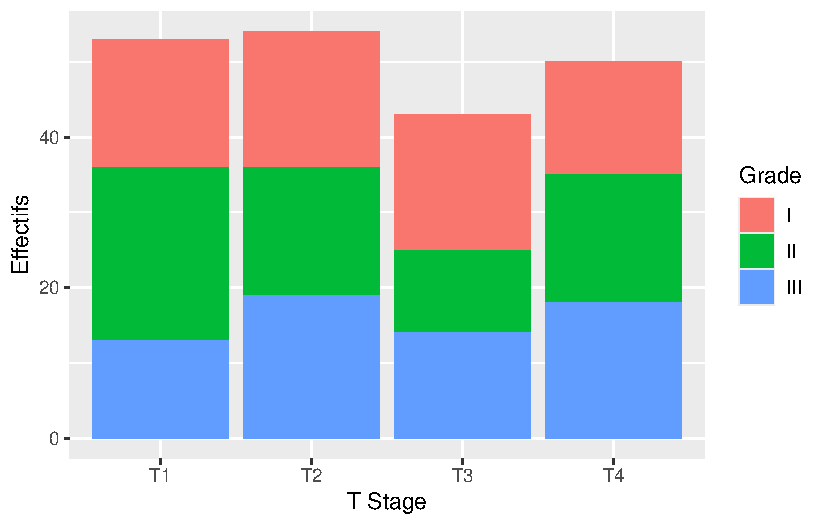
\includegraphics[keepaspectratio]{analyses/statistique-bivariee_files/figure-pdf/fig-bar-fill-1.pdf}}

}

\caption{\label{fig-bar-fill}un graphique en barres croisant deux
variables}

\end{figure}%

On peut modifier la position des barres avec le paramètre
\texttt{position}.

\begin{Shaded}
\begin{Highlighting}[]
\FunctionTok{library}\NormalTok{(ggplot2)}
\FunctionTok{ggplot}\NormalTok{(trial) }\SpecialCharTok{+}
  \FunctionTok{aes}\NormalTok{(}\AttributeTok{x =}\NormalTok{ stage, }\AttributeTok{fill =}\NormalTok{ grade) }\SpecialCharTok{+}
  \FunctionTok{geom\_bar}\NormalTok{(}\AttributeTok{position =} \StringTok{"dodge"}\NormalTok{) }\SpecialCharTok{+}
  \FunctionTok{labs}\NormalTok{(}\AttributeTok{x =} \StringTok{"T Stage"}\NormalTok{, }\AttributeTok{fill =} \StringTok{"Grade"}\NormalTok{, }\AttributeTok{y =} \StringTok{"Effectifs"}\NormalTok{)}
\end{Highlighting}
\end{Shaded}

\begin{figure}[H]

\centering{

\pandocbounded{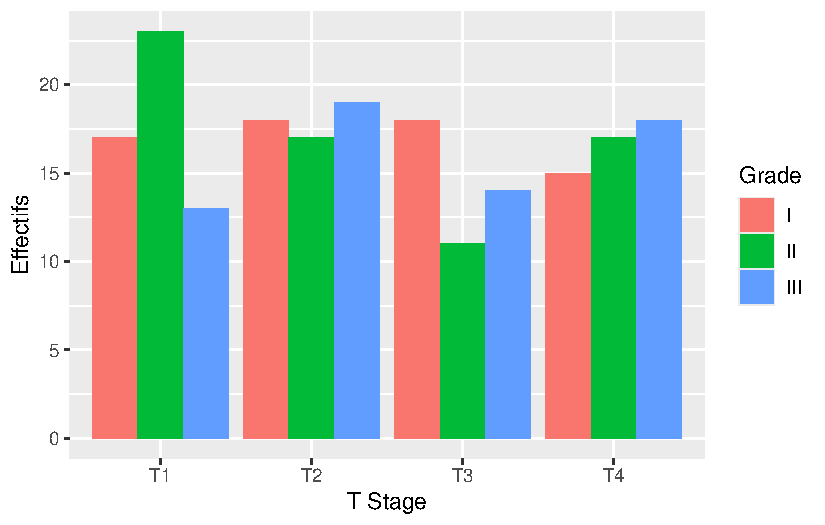
\includegraphics[keepaspectratio]{analyses/statistique-bivariee_files/figure-pdf/fig-bar-fill-dodge-1.pdf}}

}

\caption{\label{fig-bar-fill-dodge}un graphique avec des barres côte à
côte}

\end{figure}%

Pour des barres cumulées, on aura recours à
\texttt{position\ =\ "fill"}. Pour que les étiquettes de l'axe des
\texttt{y} soient représentées sous forme de pourcentages
(i.e.~\texttt{25\%} au lieu de \texttt{0.25}), on aura recours à la
fonction \texttt{scales::percent()} qui sera transmise à
\texttt{ggplot2::scale\_y\_continuous()}.

\begin{Shaded}
\begin{Highlighting}[]
\FunctionTok{library}\NormalTok{(ggplot2)}
\FunctionTok{ggplot}\NormalTok{(trial) }\SpecialCharTok{+}
  \FunctionTok{aes}\NormalTok{(}\AttributeTok{x =}\NormalTok{ stage, }\AttributeTok{fill =}\NormalTok{ grade) }\SpecialCharTok{+}
  \FunctionTok{geom\_bar}\NormalTok{(}\AttributeTok{position =} \StringTok{"fill"}\NormalTok{) }\SpecialCharTok{+}
  \FunctionTok{labs}\NormalTok{(}\AttributeTok{x =} \StringTok{"T Stage"}\NormalTok{, }\AttributeTok{fill =} \StringTok{"Grade"}\NormalTok{, }\AttributeTok{y =} \StringTok{"Proportion"}\NormalTok{) }\SpecialCharTok{+}
  \FunctionTok{scale\_y\_continuous}\NormalTok{(}\AttributeTok{labels =}\NormalTok{ scales}\SpecialCharTok{::}\NormalTok{percent)}
\end{Highlighting}
\end{Shaded}

\begin{figure}[H]

\centering{

\pandocbounded{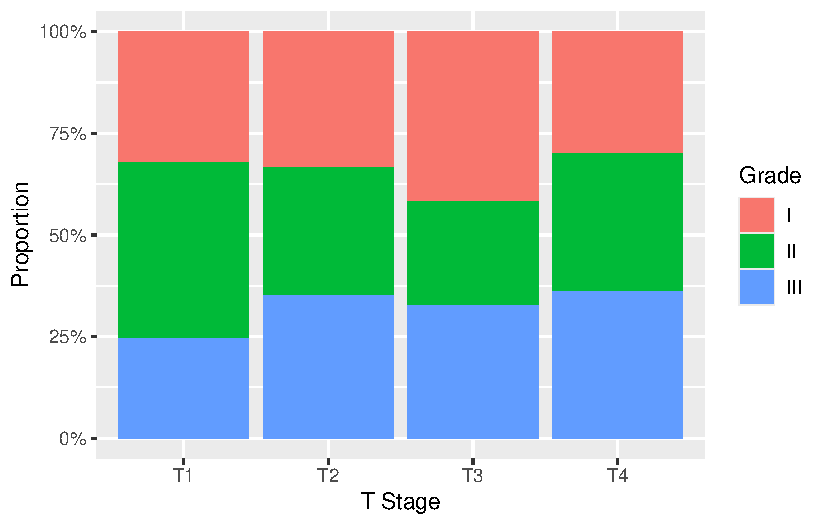
\includegraphics[keepaspectratio]{analyses/statistique-bivariee_files/figure-pdf/fig-bar-fill-dodge-2-1.pdf}}

}

\caption{\label{fig-bar-fill-dodge-2}un graphique en barres cumulées}

\end{figure}%

\begin{tcolorbox}[enhanced jigsaw, toptitle=1mm, bottomtitle=1mm, colframe=quarto-callout-tip-color-frame, toprule=.15mm, left=2mm, bottomrule=.15mm, opacitybacktitle=0.6, opacityback=0, coltitle=black, breakable, rightrule=.15mm, arc=.35mm, title=\textcolor{quarto-callout-tip-color}{\faLightbulb}\hspace{0.5em}{Ajouter des étiquettes sur un diagramme en barres}, colbacktitle=quarto-callout-tip-color!10!white, titlerule=0mm, leftrule=.75mm, colback=white]

Il est facile d'ajouter des étiquettes en ayant recours à
\texttt{ggplot2::geom\_text()}, à condition de lui passer les bons
paramètres.

Tout d'abord, il faudra préciser \texttt{stat\ =\ "count"} pour indiquer
que l'on souhaite utiliser la statistique
\texttt{ggplot2::stat\_count()} qui est celle utilisé par défaut par
\texttt{ggplot2::geom\_bar()}. C'est elle qui permets de compter le
nombre d'observations.

Il faut ensuite utiliser l'esthétique \emph{label} pour indiquer ce que
l'on souhaite afficher comme étiquettes. La fonction
\texttt{after\_stat(count)} permet d'accéder à la variable \emph{count}
calculée par \texttt{ggplot2::stat\_count()}.

Enfin, il faut indiquer la position verticale avec
\texttt{ggplot2::position\_stack()}. En précisant un ajustement de
vertical de \texttt{0.5}, on indique que l'on souhaite positionner
l'étiquette au milieu.

\begin{Shaded}
\begin{Highlighting}[]
\FunctionTok{ggplot}\NormalTok{(trial) }\SpecialCharTok{+}
  \FunctionTok{aes}\NormalTok{(}
    \AttributeTok{x =}\NormalTok{ stage, }\AttributeTok{fill =}\NormalTok{ grade, }
    \AttributeTok{label =} \FunctionTok{after\_stat}\NormalTok{(count)}
\NormalTok{  ) }\SpecialCharTok{+}
  \FunctionTok{geom\_bar}\NormalTok{() }\SpecialCharTok{+}
  \FunctionTok{geom\_text}\NormalTok{(}
    \AttributeTok{stat =} \StringTok{"count"}\NormalTok{, }
    \AttributeTok{position =} \FunctionTok{position\_stack}\NormalTok{(.}\DecValTok{5}\NormalTok{)}
\NormalTok{  )}
\end{Highlighting}
\end{Shaded}

\pandocbounded{\includegraphics[keepaspectratio]{analyses/statistique-bivariee_files/figure-pdf/unnamed-chunk-1-1.pdf}}

Pour un graphique en barres cumulées, on peut utiliser de manière
similaire \texttt{ggplot2::position\_fill()}. On ne peut afficher
directement les proportions avec \texttt{ggplot2::stat\_count()}.
Cependant, nous pouvons avoir recours à \texttt{ggstats::stat\_prop()},
déjà évoquée dans le chapitre sur la statistique univariée (cf.
Section~\ref{sec-graph-univ-var-cat}) et dont le dénominateur doit être
précisé via l'esthétique \emph{by}.

\begin{Shaded}
\begin{Highlighting}[]
\FunctionTok{library}\NormalTok{(ggstats)}
\FunctionTok{ggplot}\NormalTok{(trial) }\SpecialCharTok{+}
  \FunctionTok{aes}\NormalTok{(}
    \AttributeTok{x =}\NormalTok{ stage, }
    \AttributeTok{fill =}\NormalTok{ grade, }
    \AttributeTok{by =}\NormalTok{ stage,}
    \AttributeTok{label =}\NormalTok{ scales}\SpecialCharTok{::}\FunctionTok{percent}\NormalTok{(}\FunctionTok{after\_stat}\NormalTok{(prop), }\AttributeTok{accuracy =}\NormalTok{ .}\DecValTok{1}\NormalTok{)}
\NormalTok{  ) }\SpecialCharTok{+}
  \FunctionTok{geom\_bar}\NormalTok{(}\AttributeTok{position =} \StringTok{"fill"}\NormalTok{) }\SpecialCharTok{+}
  \FunctionTok{geom\_text}\NormalTok{(}
    \AttributeTok{stat =} \StringTok{"prop"}\NormalTok{, }
    \AttributeTok{position =} \FunctionTok{position\_fill}\NormalTok{(.}\DecValTok{5}\NormalTok{)}
\NormalTok{  ) }\SpecialCharTok{+}
  \FunctionTok{scale\_y\_continuous}\NormalTok{(}\AttributeTok{labels =}\NormalTok{ scales}\SpecialCharTok{::}\NormalTok{percent)}
\end{Highlighting}
\end{Shaded}

\pandocbounded{\includegraphics[keepaspectratio]{analyses/statistique-bivariee_files/figure-pdf/unnamed-chunk-2-1.pdf}}

On peut aussi comparer facilement deux distributions, ici la proportion
de chaque stade de cancer au sein chaque grade.

\begin{Shaded}
\begin{Highlighting}[]
\NormalTok{p }\OtherTok{\textless{}{-}} \FunctionTok{ggplot}\NormalTok{(trial) }\SpecialCharTok{+}
  \FunctionTok{aes}\NormalTok{(}
    \AttributeTok{x =}\NormalTok{ stage,}
    \AttributeTok{y =} \FunctionTok{after\_stat}\NormalTok{(prop),}
    \AttributeTok{fill =}\NormalTok{ grade, }
    \AttributeTok{by =}\NormalTok{ grade,}
    \AttributeTok{label =}\NormalTok{ scales}\SpecialCharTok{::}\FunctionTok{percent}\NormalTok{(}\FunctionTok{after\_stat}\NormalTok{(prop), }\AttributeTok{accuracy =} \DecValTok{1}\NormalTok{)}
\NormalTok{  ) }\SpecialCharTok{+}
  \FunctionTok{geom\_bar}\NormalTok{(}
    \AttributeTok{stat =} \StringTok{"prop"}\NormalTok{, }
    \AttributeTok{position =} \FunctionTok{position\_dodge}\NormalTok{(.}\DecValTok{9}\NormalTok{)}
\NormalTok{  ) }\SpecialCharTok{+}
  \FunctionTok{geom\_text}\NormalTok{(}
    \FunctionTok{aes}\NormalTok{(}\AttributeTok{y =} \FunctionTok{after\_stat}\NormalTok{(prop) }\SpecialCharTok{{-}} \FloatTok{0.01}\NormalTok{),}
    \AttributeTok{stat =} \StringTok{"prop"}\NormalTok{, }
    \AttributeTok{position =} \FunctionTok{position\_dodge}\NormalTok{(.}\DecValTok{9}\NormalTok{),}
    \AttributeTok{vjust =} \StringTok{"top"}
\NormalTok{  ) }\SpecialCharTok{+}
  \FunctionTok{scale\_y\_continuous}\NormalTok{(}\AttributeTok{labels =}\NormalTok{ scales}\SpecialCharTok{::}\NormalTok{percent)}
\NormalTok{p}
\end{Highlighting}
\end{Shaded}

\pandocbounded{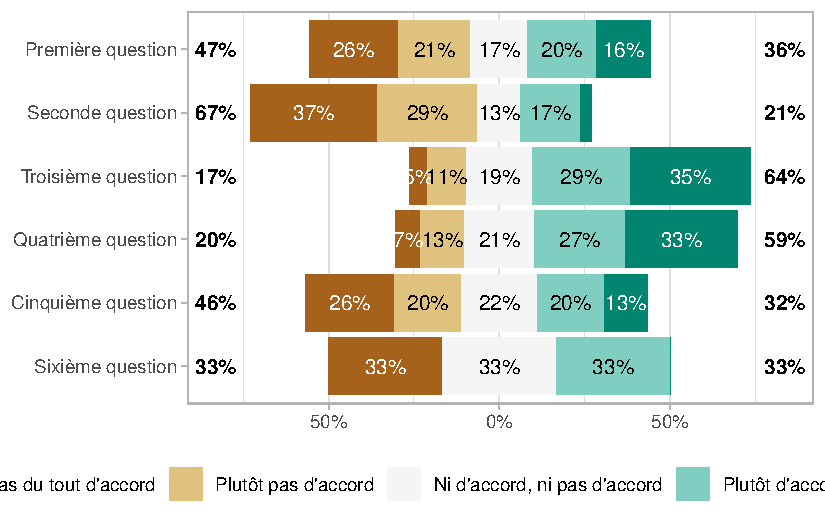
\includegraphics[keepaspectratio]{analyses/statistique-bivariee_files/figure-pdf/unnamed-chunk-3-1.pdf}}

Il est possible d'alléger le graphique en retirant des éléments
superflus.

\begin{Shaded}
\begin{Highlighting}[]
\NormalTok{p }\SpecialCharTok{+} 
  \FunctionTok{theme\_light}\NormalTok{() }\SpecialCharTok{+}
  \FunctionTok{xlab}\NormalTok{(}\StringTok{""}\NormalTok{) }\SpecialCharTok{+}
  \FunctionTok{ylab}\NormalTok{(}\StringTok{""}\NormalTok{) }\SpecialCharTok{+}
  \FunctionTok{labs}\NormalTok{(}\AttributeTok{fill =} \StringTok{""}\NormalTok{) }\SpecialCharTok{+}
  \FunctionTok{ggtitle}\NormalTok{(}\StringTok{"Distribution selon le niveau, par grade"}\NormalTok{) }\SpecialCharTok{+}
  \FunctionTok{theme}\NormalTok{(}
    \AttributeTok{panel.grid =} \FunctionTok{element\_blank}\NormalTok{(),}
    \AttributeTok{panel.border =} \FunctionTok{element\_blank}\NormalTok{(),}
    \AttributeTok{axis.text.y =} \FunctionTok{element\_blank}\NormalTok{(),}
    \AttributeTok{axis.ticks =} \FunctionTok{element\_blank}\NormalTok{(),}
    \AttributeTok{legend.position =} \StringTok{"top"}
\NormalTok{  ) }\SpecialCharTok{+}
  \FunctionTok{scale\_fill\_brewer}\NormalTok{()}
\end{Highlighting}
\end{Shaded}

\pandocbounded{\includegraphics[keepaspectratio]{analyses/statistique-bivariee_files/figure-pdf/unnamed-chunk-4-1.pdf}}

\end{tcolorbox}

Pour visualiser chaque étape du code, vous pouvez consulter le diaporama
suivant~:
\url{https://larmarange.github.io/guide-R/analyses/ressources/flipbook-geom_bar-dodge.html}

\begin{tcolorbox}[enhanced jigsaw, toptitle=1mm, bottomtitle=1mm, colframe=quarto-callout-tip-color-frame, toprule=.15mm, left=2mm, bottomrule=.15mm, opacitybacktitle=0.6, opacityback=0, coltitle=black, breakable, rightrule=.15mm, arc=.35mm, title=\textcolor{quarto-callout-tip-color}{\faLightbulb}\hspace{0.5em}{Diagramme alluvial}, colbacktitle=quarto-callout-tip-color!10!white, titlerule=0mm, leftrule=.75mm, colback=white]

Une représentation alternative du croisement de deux variables est à
d'avoir recours à un diagramme alluvial\footnotemark{}. Ce type de
graphique est particulièrement adapté pour des données temporelles, par
exemple du type avant / après. Il peut également être étendu à un plus
grand nombre d'étapes. Ci-dessous, un exemple reposants sur le package
\texttt{\{ggalluvial\}}.

\begin{Shaded}
\begin{Highlighting}[]
\FunctionTok{library}\NormalTok{(ggalluvial)}
\FunctionTok{ggplot}\NormalTok{(trial) }\SpecialCharTok{+}
  \FunctionTok{aes}\NormalTok{(}\AttributeTok{axis1 =}\NormalTok{ grade, }\AttributeTok{axis2 =}\NormalTok{ stage) }\SpecialCharTok{+}
  \FunctionTok{geom\_flow}\NormalTok{(}\AttributeTok{mapping =} \FunctionTok{aes}\NormalTok{(}\AttributeTok{fill =}\NormalTok{ grade)) }\SpecialCharTok{+}
  \FunctionTok{geom\_stratum}\NormalTok{() }\SpecialCharTok{+}
  \FunctionTok{geom\_text}\NormalTok{(}\AttributeTok{stat =} \StringTok{"stratum"}\NormalTok{, }\FunctionTok{aes}\NormalTok{(}\AttributeTok{label =} \FunctionTok{after\_stat}\NormalTok{(stratum))) }\SpecialCharTok{+}
  \FunctionTok{scale\_x\_discrete}\NormalTok{(}\AttributeTok{limits =} \FunctionTok{c}\NormalTok{(}\StringTok{"Grade"}\NormalTok{, }\StringTok{" T Stage"}\NormalTok{)) }\SpecialCharTok{+}
  \FunctionTok{theme\_minimal}\NormalTok{()}
\end{Highlighting}
\end{Shaded}

\pandocbounded{\includegraphics[keepaspectratio]{analyses/statistique-bivariee_files/figure-pdf/unnamed-chunk-5-1.pdf}}

\end{tcolorbox}

\footnotetext{Un graphique alluvial est une variation d'un graphique de
Sankey. Usuellement, un graphique de Sankey espace verticalement les
différents statuts d'une même étape, tandis qu'il n'y a pas d'espace
vertical dans un diagramme alluvial. Le package \texttt{\{ggsankey\}}
propose une implémentation à la fois des diagrammes de Sankey des
diagrammes alluviaux. Ce package n'est cependant pas disponible sur
\textbf{CRAN} et doit être installé manuellement depuis GitHub. Pour un
diagramme de Sankey, on pourra également avoir recours à
\texttt{ggforce::geom\_parallel\_sets()} du package
\texttt{\{ggforce\}}. Cette fonction nécessite une réorganisation des
données dans un format long au préalable.}

\subsection{Représentations graphiques (variable
binaire)}\label{repruxe9sentations-graphiques-variable-binaire}

Pour croiser une proportion simple (variable binaire), on pourra avoir
recours à la fonction \texttt{guideR::plot\_proportions()} fournie par
\texttt{\{guideR\}}, le package compagnon de \emph{guide-R}. Pour cela,
on indiquera une condition définissant la proportion à représenter et,
éventuellement, une liste de variables de croisement. Cette fonction a
l'avantage de représenter également les intervalles de confiance à 95\%
ainsi que des tests de comparaison (voir ci-après). Pour plus
d'information sur les différentes options disponibles, voir
l'\href{https://larmarange.github.io/guideR/reference/plot_proportions.html}{aide
de la fonction}.

\begin{Shaded}
\begin{Highlighting}[]
\FunctionTok{library}\NormalTok{(guideR)}
\NormalTok{trial }\SpecialCharTok{|\textgreater{}} 
  \FunctionTok{plot\_proportions}\NormalTok{(}
\NormalTok{    death }\SpecialCharTok{==} \DecValTok{1}\NormalTok{,}
    \AttributeTok{by =} \FunctionTok{c}\NormalTok{(grade, stage),}
    \AttributeTok{fill =} \StringTok{"darksalmon"}\NormalTok{,}
    \AttributeTok{show\_overall\_line =} \ConstantTok{TRUE}
\NormalTok{  )}
\end{Highlighting}
\end{Shaded}

\pandocbounded{\includegraphics[keepaspectratio]{analyses/statistique-bivariee_files/figure-pdf/unnamed-chunk-6-1.pdf}}

\subsection{Calcul manuel}\label{calcul-manuel-1}

Les deux fonctions de base permettant le calcul d'un tri à plat sont
\texttt{table()} et \texttt{xtabs()} (cf.
Section~\ref{sec-table-univariee}). Ces mêmes fonctions permettent le
calcul du tri croisé de deux variables (ou plus). Pour \texttt{table()},
on passera les deux vecteurs à croisés, tandis que pour \texttt{xtabs()}
on décrira le tableau attendu à l'aide d'une formule.

\begin{Shaded}
\begin{Highlighting}[]
\FunctionTok{table}\NormalTok{(trial}\SpecialCharTok{$}\NormalTok{stage, trial}\SpecialCharTok{$}\NormalTok{grade)}
\end{Highlighting}
\end{Shaded}

\begin{verbatim}
    
      I II III
  T1 17 23  13
  T2 18 17  19
  T3 18 11  14
  T4 15 17  18
\end{verbatim}

\begin{Shaded}
\begin{Highlighting}[]
\NormalTok{tab }\OtherTok{\textless{}{-}} \FunctionTok{xtabs}\NormalTok{(}\SpecialCharTok{\textasciitilde{}}\NormalTok{ stage }\SpecialCharTok{+}\NormalTok{ grade, }\AttributeTok{data =}\NormalTok{ trial)}
\NormalTok{tab}
\end{Highlighting}
\end{Shaded}

\begin{verbatim}
     grade
stage  I II III
   T1 17 23  13
   T2 18 17  19
   T3 18 11  14
   T4 15 17  18
\end{verbatim}

Le tableau obtenu est basique et ne contient que les effectifs. La
fonction \texttt{addmargins()} permet d'ajouter les totaux par ligne et
par colonne.

\begin{Shaded}
\begin{Highlighting}[]
\NormalTok{tab }\SpecialCharTok{|\textgreater{}} \FunctionTok{addmargins}\NormalTok{()}
\end{Highlighting}
\end{Shaded}

\begin{verbatim}
     grade
stage   I  II III Sum
  T1   17  23  13  53
  T2   18  17  19  54
  T3   18  11  14  43
  T4   15  17  18  50
  Sum  68  68  64 200
\end{verbatim}

Pour le calcul des pourcentages, le plus simple est d'avoir recours au
package \texttt{\{questionr\}} qui fournit les fonctions
\texttt{questionr::cprop()}, \texttt{questionr::rprop()} et
\texttt{questionr::prop()} qui permettent de calculer, respectivement,
les pourcentages en colonne, en ligne et totaux.

\begin{Shaded}
\begin{Highlighting}[]
\NormalTok{questionr}\SpecialCharTok{::}\FunctionTok{cprop}\NormalTok{(tab)}
\end{Highlighting}
\end{Shaded}

\begin{verbatim}
       grade
stage   I     II    III   Ensemble
  T1     25.0  33.8  20.3  26.5   
  T2     26.5  25.0  29.7  27.0   
  T3     26.5  16.2  21.9  21.5   
  T4     22.1  25.0  28.1  25.0   
  Total 100.0 100.0 100.0 100.0   
\end{verbatim}

\begin{Shaded}
\begin{Highlighting}[]
\NormalTok{questionr}\SpecialCharTok{::}\FunctionTok{rprop}\NormalTok{(tab)}
\end{Highlighting}
\end{Shaded}

\begin{verbatim}
          grade
stage      I     II    III   Total
  T1        32.1  43.4  24.5 100.0
  T2        33.3  31.5  35.2 100.0
  T3        41.9  25.6  32.6 100.0
  T4        30.0  34.0  36.0 100.0
  Ensemble  34.0  34.0  32.0 100.0
\end{verbatim}

\begin{Shaded}
\begin{Highlighting}[]
\NormalTok{questionr}\SpecialCharTok{::}\FunctionTok{prop}\NormalTok{(tab)}
\end{Highlighting}
\end{Shaded}

\begin{verbatim}
       grade
stage   I     II    III   Total
  T1      8.5  11.5   6.5  26.5
  T2      9.0   8.5   9.5  27.0
  T3      9.0   5.5   7.0  21.5
  T4      7.5   8.5   9.0  25.0
  Total  34.0  34.0  32.0 100.0
\end{verbatim}

Si l'on a besoin des différents résultats dans un tableau de données, le
plus simple avec d'avoir recours à la fonction
\texttt{guideR::proportion()} fournie dans \texttt{\{guideR\}} le
package compagnon de \emph{guide-R}.

Si on lui passe une simple liste des variables, on obtient des
pourcentages du total.

\begin{Shaded}
\begin{Highlighting}[]
\FunctionTok{library}\NormalTok{(guideR)}
\NormalTok{trial }\SpecialCharTok{|\textgreater{}} \FunctionTok{proportion}\NormalTok{(stage, grade)}
\end{Highlighting}
\end{Shaded}

\begin{verbatim}
# A tibble: 12 x 5
   stage grade     n     N  prop
   <fct> <fct> <int> <int> <dbl>
 1 T1    I        17   200   8.5
 2 T1    II       23   200  11.5
 3 T1    III      13   200   6.5
 4 T2    I        18   200   9  
 5 T2    II       17   200   8.5
 6 T2    III      19   200   9.5
 7 T3    I        18   200   9  
 8 T3    II       11   200   5.5
 9 T3    III      14   200   7  
10 T4    I        15   200   7.5
11 T4    II       17   200   8.5
12 T4    III      18   200   9  
\end{verbatim}

Mais l'on peut contrôler la manière de calculer les pourcentages avec le
paramètre \texttt{.by}. Ainsi, pour la répartition par stade selon le
grade~:

\begin{Shaded}
\begin{Highlighting}[]
\NormalTok{trial }\SpecialCharTok{|\textgreater{}} \FunctionTok{proportion}\NormalTok{(stage, }\AttributeTok{.by =}\NormalTok{ grade)}
\end{Highlighting}
\end{Shaded}

\begin{verbatim}
# A tibble: 12 x 5
# Groups:   grade [3]
   grade stage     n     N  prop
   <fct> <fct> <int> <int> <dbl>
 1 I     T1       17    68  25  
 2 I     T2       18    68  26.5
 3 I     T3       18    68  26.5
 4 I     T4       15    68  22.1
 5 II    T1       23    68  33.8
 6 II    T2       17    68  25  
 7 II    T3       11    68  16.2
 8 II    T4       17    68  25  
 9 III   T1       13    64  20.3
10 III   T2       19    64  29.7
11 III   T3       14    64  21.9
12 III   T4       18    64  28.1
\end{verbatim}

La fonction \texttt{guideR::proportion()} peut également être utilisée
pour des tableaux à 3 entrées ou plus.

\subsection{Test du Chi² et
dérivés}\label{test-du-chiuxb2-et-duxe9rivuxe9s}

Dans le cadre d'un tableau croisé, on peut tester l'existence d'un lien
entre les modalités de deux variables, avec le très classique test du
Chi² (parfois écrit χ² ou Chi²). Pour une présentation plus détaillée du
test, on pourra se référer à ce
\href{https://github.com/juba/archive_doc_khi2/raw/master/khi2.pdf}{cours
de Julien Barnier}.

Le test du Chi² peut se calculer très facilement avec la fonction
\texttt{chisq.test()} appliquée au tableau obtenu avec \texttt{table()}
ou \texttt{xtabs()}.

\begin{Shaded}
\begin{Highlighting}[]
\NormalTok{tab }\OtherTok{\textless{}{-}} \FunctionTok{xtabs}\NormalTok{(}\SpecialCharTok{\textasciitilde{}}\NormalTok{ stage }\SpecialCharTok{+}\NormalTok{ grade, }\AttributeTok{data =}\NormalTok{ trial)}
\NormalTok{tab}
\end{Highlighting}
\end{Shaded}

\begin{verbatim}
     grade
stage  I II III
   T1 17 23  13
   T2 18 17  19
   T3 18 11  14
   T4 15 17  18
\end{verbatim}

\begin{Shaded}
\begin{Highlighting}[]
\FunctionTok{chisq.test}\NormalTok{(tab)}
\end{Highlighting}
\end{Shaded}

\begin{verbatim}

    Pearson's Chi-squared test

data:  tab
X-squared = 4.8049, df = 6, p-value = 0.5691
\end{verbatim}

Si l'on est adepte de \texttt{\{gtsummary\}}, il suffit d'appliquer
\texttt{gtsummary::add\_p()} au tableau produit avec
\texttt{gtsummary::tbl\_summary()}.

\begin{Shaded}
\begin{Highlighting}[]
\NormalTok{trial }\SpecialCharTok{|\textgreater{}} 
  \FunctionTok{tbl\_summary}\NormalTok{(}
    \AttributeTok{include =}\NormalTok{ stage,}
    \AttributeTok{by =}\NormalTok{ grade}
\NormalTok{  ) }\SpecialCharTok{|\textgreater{}} 
  \FunctionTok{add\_p}\NormalTok{()}
\end{Highlighting}
\end{Shaded}

\begin{table}

\caption{\label{tbl-add_p}un tableau croisé avec test du khi²}

\centering{

\fontsize{12.0pt}{14.4pt}\selectfont
\begin{tabular*}{\linewidth}{@{\extracolsep{\fill}}lcccc}
\toprule
\textbf{Caractéristique} & \textbf{I}  N = 68\textsuperscript{\textit{1}} & \textbf{II}  N = 68\textsuperscript{\textit{1}} & \textbf{III}  N = 64\textsuperscript{\textit{1}} & \textbf{p-valeur}\textsuperscript{\textit{2}} \\ 
\midrule\addlinespace[2.5pt]
T Stage &  &  &  & 0,6 \\ 
    T1 & 17 (25\%) & 23 (34\%) & 13 (20\%) &  \\ 
    T2 & 18 (26\%) & 17 (25\%) & 19 (30\%) &  \\ 
    T3 & 18 (26\%) & 11 (16\%) & 14 (22\%) &  \\ 
    T4 & 15 (22\%) & 17 (25\%) & 18 (28\%) &  \\ 
\bottomrule
\end{tabular*}
\begin{minipage}{\linewidth}
\textsuperscript{\textit{1}}n (\%)\\
\textsuperscript{\textit{2}}test du khi-deux d'indépendance\\
\end{minipage}

}

\end{table}%

Dans notre exemple, les deux variables \emph{stage} et \emph{grade} ne
sont clairement pas corrélées.

Un test alternatif est le test exact de Fisher. Il s'obtient aisément
avec \texttt{fisher.test()} ou bien en le spécifiant via l'argument
\texttt{test} de \texttt{gtsummary::add\_p()}.

\begin{Shaded}
\begin{Highlighting}[]
\NormalTok{tab }\OtherTok{\textless{}{-}} \FunctionTok{xtabs}\NormalTok{(}\SpecialCharTok{\textasciitilde{}}\NormalTok{ stage }\SpecialCharTok{+}\NormalTok{ grade, }\AttributeTok{data =}\NormalTok{ trial)}
\FunctionTok{fisher.test}\NormalTok{(tab)}
\end{Highlighting}
\end{Shaded}

\begin{verbatim}

    Fisher's Exact Test for Count Data

data:  tab
p-value = 0.5801
alternative hypothesis: two.sided
\end{verbatim}

\begin{Shaded}
\begin{Highlighting}[]
\NormalTok{trial }\SpecialCharTok{|\textgreater{}} 
  \FunctionTok{tbl\_summary}\NormalTok{(}
    \AttributeTok{include =}\NormalTok{ stage,}
    \AttributeTok{by =}\NormalTok{ grade}
\NormalTok{  ) }\SpecialCharTok{|\textgreater{}} 
  \FunctionTok{add\_p}\NormalTok{(}\AttributeTok{test =} \FunctionTok{all\_categorical}\NormalTok{() }\SpecialCharTok{\textasciitilde{}} \StringTok{"fisher.test"}\NormalTok{)}
\end{Highlighting}
\end{Shaded}

\begin{table}

\caption{\label{tbl-add_p-fisher}un tableau croisé avec test exact de
Fisher}

\centering{

\fontsize{12.0pt}{14.4pt}\selectfont
\begin{tabular*}{\linewidth}{@{\extracolsep{\fill}}lcccc}
\toprule
\textbf{Caractéristique} & \textbf{I}  N = 68\textsuperscript{\textit{1}} & \textbf{II}  N = 68\textsuperscript{\textit{1}} & \textbf{III}  N = 64\textsuperscript{\textit{1}} & \textbf{p-valeur}\textsuperscript{\textit{2}} \\ 
\midrule\addlinespace[2.5pt]
T Stage &  &  &  & 0,6 \\ 
    T1 & 17 (25\%) & 23 (34\%) & 13 (20\%) &  \\ 
    T2 & 18 (26\%) & 17 (25\%) & 19 (30\%) &  \\ 
    T3 & 18 (26\%) & 11 (16\%) & 14 (22\%) &  \\ 
    T4 & 15 (22\%) & 17 (25\%) & 18 (28\%) &  \\ 
\bottomrule
\end{tabular*}
\begin{minipage}{\linewidth}
\textsuperscript{\textit{1}}n (\%)\\
\textsuperscript{\textit{2}}test exact de Fisher\\
\end{minipage}

}

\end{table}%

\begin{tcolorbox}[enhanced jigsaw, toptitle=1mm, bottomtitle=1mm, colframe=quarto-callout-note-color-frame, toprule=.15mm, left=2mm, bottomrule=.15mm, opacitybacktitle=0.6, opacityback=0, coltitle=black, breakable, rightrule=.15mm, arc=.35mm, title=\textcolor{quarto-callout-note-color}{\faInfo}\hspace{0.5em}{Note}, colbacktitle=quarto-callout-note-color!10!white, titlerule=0mm, leftrule=.75mm, colback=white]

Formellement, le test de Fisher suppose que les marges du tableau
(totaux lignes et colonnes) sont fixées, puisqu'il repose sur une loi
hypergéométrique, et donc celui-ci se prête plus au cas des situations
expérimentales (plans d'expérience, essais cliniques) qu'au cas des
données tirées d'études observationnelles.

En pratique, le test du Chi² étant assez robuste quant aux déviations
par rapport aux hypothèses d'applications du test (effectifs théoriques
supérieurs ou égaux à 5), le test de Fisher présente en général peu
d'intérêt dans le cas de l'analyse des tableaux de contingence.

\end{tcolorbox}

\subsection{Comparaison de deux
proportions}\label{comparaison-de-deux-proportions}

Pour comparer deux proportions, la fonction de base est
\texttt{prop.test()} à laquelle on passera un tableau à 2×2 dimensions.

\begin{Shaded}
\begin{Highlighting}[]
\NormalTok{tab }\OtherTok{\textless{}{-}} \FunctionTok{xtabs}\NormalTok{(}\SpecialCharTok{\textasciitilde{}} \FunctionTok{I}\NormalTok{(stage }\SpecialCharTok{==} \StringTok{"T1"}\NormalTok{) }\SpecialCharTok{+}\NormalTok{ trt, }\AttributeTok{data =}\NormalTok{ trial)}
\NormalTok{tab }\SpecialCharTok{|\textgreater{}}\NormalTok{ questionr}\SpecialCharTok{::}\FunctionTok{cprop}\NormalTok{()}
\end{Highlighting}
\end{Shaded}

\begin{verbatim}
                trt
I(stage == "T1") Drug A Drug B Ensemble
           FALSE  71.4   75.5   73.5   
           TRUE   28.6   24.5   26.5   
           Total 100.0  100.0  100.0   
\end{verbatim}

\begin{Shaded}
\begin{Highlighting}[]
\NormalTok{tab }\SpecialCharTok{|\textgreater{}} \FunctionTok{prop.test}\NormalTok{()}
\end{Highlighting}
\end{Shaded}

\begin{verbatim}

    2-sample test for equality of proportions with continuity correction

data:  tab
X-squared = 0.24047, df = 1, p-value = 0.6239
alternative hypothesis: two.sided
95 percent confidence interval:
 -0.2217278  0.1175050
sample estimates:
   prop 1    prop 2 
0.4761905 0.5283019 
\end{verbatim}

Il est également envisageable d'avoir recours à un test exact de Fisher.
Dans le cas d'un tableau à 2×2 dimensions, le test exact de Fisher ne
teste pas si les deux proportions sont différents, mais plutôt si leur
\href{https://fr.wikipedia.org/wiki/Odds_ratio}{\emph{odds ratio}} (qui
est d'ailleurs renvoyé par la fonction) est différent de 1.

\begin{Shaded}
\begin{Highlighting}[]
\FunctionTok{fisher.test}\NormalTok{(tab)}
\end{Highlighting}
\end{Shaded}

\begin{verbatim}

    Fisher's Exact Test for Count Data

data:  tab
p-value = 0.5263
alternative hypothesis: true odds ratio is not equal to 1
95 percent confidence interval:
 0.4115109 1.5973635
sample estimates:
odds ratio 
 0.8125409 
\end{verbatim}

Mais le plus simple reste encore d'avoir recours à
\texttt{\{gtsummary\}} et à sa fonction
\texttt{gtsummary::add\_difference()} que l'on peut appliquer à un
tableau où le paramètre \texttt{by} n'a que deux modalités. Pour la
différence de proportions, il faut que les variables transmises à
\texttt{include} soit dichotomiques.

\begin{Shaded}
\begin{Highlighting}[]
\NormalTok{trial }\SpecialCharTok{|\textgreater{}} 
  \FunctionTok{tbl\_summary}\NormalTok{(}
    \AttributeTok{by =}\NormalTok{ trt,}
    \AttributeTok{include =}\NormalTok{ response}
\NormalTok{  ) }\SpecialCharTok{|\textgreater{}} 
  \FunctionTok{add\_difference}\NormalTok{()}
\end{Highlighting}
\end{Shaded}

\begin{table}

\caption{\label{tbl-add_difference}différence entre deux proportions}

\centering{

\fontsize{12.0pt}{14.4pt}\selectfont
\begin{tabular*}{\linewidth}{@{\extracolsep{\fill}}lccccc}
\toprule
\textbf{Caractéristique} & \textbf{Drug A}  N = 98\textsuperscript{\textit{1}} & \textbf{Drug B}  N = 102\textsuperscript{\textit{1}} & \textbf{Différence}\textsuperscript{\textit{2}} & \textbf{95\% IC}\textsuperscript{\textit{2}} & \textbf{p-valeur}\textsuperscript{\textit{2}} \\ 
\midrule\addlinespace[2.5pt]
Tumor Response & 28 (29\%) & 33 (34\%) & -4,2% & -18% – 9,9% & 0,6 \\ 
    Manquant & 3 & 4 &  &  &  \\ 
\bottomrule
\end{tabular*}
\begin{minipage}{\linewidth}
\textsuperscript{\textit{1}}n (\%)\\
\textsuperscript{\textit{2}}2-sample test for equality of proportions with continuity correction\\
Abréviation: IC = intervalle de confiance\\
\end{minipage}

}

\end{table}%

\textbf{Attention~:} si l'on passe une variable catégorielle à trois
modalités ou plus, c'est la différence des moyennes standardisées
(globale pour la variable) qui sera calculée et non la différence des
proportions dans chaque groupe.

\begin{Shaded}
\begin{Highlighting}[]
\NormalTok{trial }\SpecialCharTok{|\textgreater{}} 
  \FunctionTok{tbl\_summary}\NormalTok{(}
    \AttributeTok{by =}\NormalTok{ trt,}
    \AttributeTok{include =}\NormalTok{ grade}
\NormalTok{  ) }\SpecialCharTok{|\textgreater{}} 
  \FunctionTok{add\_difference}\NormalTok{()}
\end{Highlighting}
\end{Shaded}

\begin{verbatim}
The following errors were returned during `add_difference()`:
x For variable `grade` (`trt`) and "estimate" statistic: The package "smd" (>=
  0.6.6) is required.
\end{verbatim}

\begin{table}

\caption{\label{tbl-add_difference-2}différence moyenne standardisée}

\centering{

\fontsize{12.0pt}{14.4pt}\selectfont
\begin{tabular*}{\linewidth}{@{\extracolsep{\fill}}lccc}
\toprule
\textbf{Caractéristique} & \textbf{Drug A}  N = 98\textsuperscript{\textit{1}} & \textbf{Drug B}  N = 102\textsuperscript{\textit{1}} & \textbf{Différence} \\ 
\midrule\addlinespace[2.5pt]
Grade &  &  &  \\ 
    I & 35 (36\%) & 33 (32\%) &  \\ 
    II & 32 (33\%) & 36 (35\%) &  \\ 
    III & 31 (32\%) & 33 (32\%) &  \\ 
\bottomrule
\end{tabular*}
\begin{minipage}{\linewidth}
\textsuperscript{\textit{1}}n (\%)\\
\end{minipage}

}

\end{table}%

Pour calculer la différence des proportions pour chaque modalité de
\emph{grade}, il est nécessaire de transformer, en amont, la variable
catégorielle \emph{grade} en trois variables dichotomiques (de type
oui/non, une par modalité), ce qui peut se faire facilement avec la
fonction \texttt{fastDummies::dummy\_cols()} de l'extension
\texttt{\{fastDummies\}}.

\begin{Shaded}
\begin{Highlighting}[]
\NormalTok{trial }\SpecialCharTok{|\textgreater{}} 
\NormalTok{  fastDummies}\SpecialCharTok{::}\FunctionTok{dummy\_cols}\NormalTok{(}\StringTok{"grade"}\NormalTok{) }\SpecialCharTok{|\textgreater{}} 
  \FunctionTok{tbl\_summary}\NormalTok{(}
    \AttributeTok{by =}\NormalTok{ trt,}
    \AttributeTok{include =} \FunctionTok{starts\_with}\NormalTok{(}\StringTok{"grade\_"}\NormalTok{),}
    \AttributeTok{digits =} \SpecialCharTok{\textasciitilde{}} \FunctionTok{c}\NormalTok{(}\DecValTok{0}\NormalTok{, }\DecValTok{1}\NormalTok{)}
\NormalTok{  ) }\SpecialCharTok{|\textgreater{}} 
  \FunctionTok{add\_difference}\NormalTok{()}
\end{Highlighting}
\end{Shaded}

\begin{table}

\caption{\label{tbl-add_difference-3}différence entre proportions avec
création de variables dichotomiques}

\centering{

\fontsize{12.0pt}{14.4pt}\selectfont
\begin{tabular*}{\linewidth}{@{\extracolsep{\fill}}lccccc}
\toprule
\textbf{Caractéristique} & \textbf{Drug A}  N = 98\textsuperscript{\textit{1}} & \textbf{Drug B}  N = 102\textsuperscript{\textit{1}} & \textbf{Différence}\textsuperscript{\textit{2}} & \textbf{95\% IC}\textsuperscript{\textit{2}} & \textbf{p-valeur}\textsuperscript{\textit{2}} \\ 
\midrule\addlinespace[2.5pt]
grade\_I & 35 (35,7\%) & 33 (32,4\%) & 3,4% & -11% – 17% & 0,7 \\ 
grade\_II & 32 (32,7\%) & 36 (35,3\%) & -2,6% & -17% – 11% & 0,8 \\ 
grade\_III & 31 (31,6\%) & 33 (32,4\%) & -0,72% & -14% – 13% & >0,9 \\ 
\bottomrule
\end{tabular*}
\begin{minipage}{\linewidth}
\textsuperscript{\textit{1}}n (\%)\\
\textsuperscript{\textit{2}}2-sample test for equality of proportions with continuity correction\\
Abréviation: IC = intervalle de confiance\\
\end{minipage}

}

\end{table}%

\section{Une variable continue selon une variable
catégorielle}\label{une-variable-continue-selon-une-variable-catuxe9gorielle}

\subsection{\texorpdfstring{Tableau comparatif avec
\texttt{gtsummary}}{Tableau comparatif avec gtsummary}}\label{tableau-comparatif-avec-gtsummary}

Dans le chapitre sur la statistique univariée (cf.
Section~\ref{sec-tri-a-plat}), nous avons abordé comment afficher les
statistiques descriptives d'une variable continue avec
\texttt{gtsummary::tbl\_summary()}. Pour comparer une variable continue
selon plusieurs groupes définis par une variable catégorielle, il suffit
d'utiliser le paramètre \texttt{by}~:

\begin{Shaded}
\begin{Highlighting}[]
\NormalTok{trial }\SpecialCharTok{|\textgreater{}} 
  \FunctionTok{tbl\_summary}\NormalTok{(}
    \AttributeTok{include =}\NormalTok{ age,}
    \AttributeTok{by =}\NormalTok{ grade}
\NormalTok{  )}
\end{Highlighting}
\end{Shaded}

\begin{table}

\caption{\label{tbl-by-cont}âge médian et intervalle interquartile selon
le grade}

\centering{

\fontsize{12.0pt}{14.4pt}\selectfont
\begin{tabular*}{\linewidth}{@{\extracolsep{\fill}}lccc}
\toprule
\textbf{Caractéristique} & \textbf{I}  N = 68\textsuperscript{\textit{1}} & \textbf{II}  N = 68\textsuperscript{\textit{1}} & \textbf{III}  N = 64\textsuperscript{\textit{1}} \\ 
\midrule\addlinespace[2.5pt]
Age & 47 (37 – 56) & 49 (37 – 57) & 47 (38 – 58) \\ 
    Manquant & 2 & 6 & 3 \\ 
\bottomrule
\end{tabular*}
\begin{minipage}{\linewidth}
\textsuperscript{\textit{1}}Médiane (Q1 -- Q3)\\
\end{minipage}

}

\end{table}%

La fonction \texttt{gtsummary::add\_overall()} permet d'ajouter une
colonne total et \texttt{gtsummary::modify\_spanning\_header()}
peut-être utilisé pour ajouter un en-tête de colonne.

\begin{Shaded}
\begin{Highlighting}[]
\NormalTok{trial }\SpecialCharTok{|\textgreater{}} 
  \FunctionTok{tbl\_summary}\NormalTok{(}
    \AttributeTok{include =}\NormalTok{ age,}
    \AttributeTok{by =}\NormalTok{ grade}
\NormalTok{  ) }\SpecialCharTok{|\textgreater{}} 
  \FunctionTok{add\_overall}\NormalTok{(}\AttributeTok{last =} \ConstantTok{TRUE}\NormalTok{) }\SpecialCharTok{|\textgreater{}} 
  \FunctionTok{modify\_spanning\_header}\NormalTok{(}
    \FunctionTok{all\_stat\_cols}\NormalTok{(}\AttributeTok{stat\_0 =} \ConstantTok{FALSE}\NormalTok{) }\SpecialCharTok{\textasciitilde{}} \StringTok{"**Grade**"}
\NormalTok{  )}
\end{Highlighting}
\end{Shaded}

\begin{table}

\caption{\label{tbl-by-cont-2}âge médian et intervalle interquartile
selon le grade}

\centering{

\fontsize{12.0pt}{14.4pt}\selectfont
\begin{tabular*}{\linewidth}{@{\extracolsep{\fill}}lcccc}
\toprule
 & \multicolumn{3}{c}{\textbf{Grade}} &  \\ 
\cmidrule(lr){2-4}
\textbf{Caractéristique} & \textbf{I}  N = 68\textsuperscript{\textit{1}} & \textbf{II}  N = 68\textsuperscript{\textit{1}} & \textbf{III}  N = 64\textsuperscript{\textit{1}} & \textbf{Overall}  N = 200\textsuperscript{\textit{1}} \\ 
\midrule\addlinespace[2.5pt]
Age & 47 (37 – 56) & 49 (37 – 57) & 47 (38 – 58) & 47 (38 – 57) \\ 
    Manquant & 2 & 6 & 3 & 11 \\ 
\bottomrule
\end{tabular*}
\begin{minipage}{\linewidth}
\textsuperscript{\textit{1}}Médiane (Q1 -- Q3)\\
\end{minipage}

}

\end{table}%

Comme pour un tri à plat, on peut personnaliser les statistiques à
afficher avec \texttt{statistic}.

\begin{Shaded}
\begin{Highlighting}[]
\NormalTok{trial }\SpecialCharTok{|\textgreater{}} 
  \FunctionTok{tbl\_summary}\NormalTok{(}
    \AttributeTok{include =}\NormalTok{ age,}
    \AttributeTok{by =}\NormalTok{ grade,}
    \AttributeTok{statistic =} \FunctionTok{all\_continuous}\NormalTok{() }\SpecialCharTok{\textasciitilde{}} \StringTok{"\{mean\} (\{sd\})"}\NormalTok{,}
    \AttributeTok{digits =} \FunctionTok{all\_continuous}\NormalTok{() }\SpecialCharTok{\textasciitilde{}} \FunctionTok{c}\NormalTok{(}\DecValTok{1}\NormalTok{, }\DecValTok{1}\NormalTok{)}
\NormalTok{  ) }\SpecialCharTok{|\textgreater{}} 
  \FunctionTok{add\_overall}\NormalTok{(}\AttributeTok{last =} \ConstantTok{TRUE}\NormalTok{)}
\end{Highlighting}
\end{Shaded}

\begin{table}

\caption{\label{tbl-by-cont-3}âge moyen et écart-type selon le grade}

\centering{

\fontsize{12.0pt}{14.4pt}\selectfont
\begin{tabular*}{\linewidth}{@{\extracolsep{\fill}}lcccc}
\toprule
\textbf{Caractéristique} & \textbf{I}  N = 68\textsuperscript{\textit{1}} & \textbf{II}  N = 68\textsuperscript{\textit{1}} & \textbf{III}  N = 64\textsuperscript{\textit{1}} & \textbf{Overall}  N = 200\textsuperscript{\textit{1}} \\ 
\midrule\addlinespace[2.5pt]
Age & 46,2 (15,2) & 47,5 (13,7) & 48,1 (14,1) & 47,2 (14,3) \\ 
    Manquant & 2 & 6 & 3 & 11 \\ 
\bottomrule
\end{tabular*}
\begin{minipage}{\linewidth}
\textsuperscript{\textit{1}}Moyenne (ET)\\
\end{minipage}

}

\end{table}%

\subsection{Représentations
graphiques}\label{repruxe9sentations-graphiques}

La moyenne ou la médiane sont des indicateurs centraux et ne suffisent
pas à rendre compte des différences de distribution d'une variable
continue entre plusieurs sous-groupes.

Une représentation usuelle pour comparer deux distributions consiste à
avoir recours à des boîtes à moustaches que l'on obtient avec
\texttt{ggplot2::geom\_boxplot()}.

\begin{Shaded}
\begin{Highlighting}[]
\FunctionTok{ggplot}\NormalTok{(trial) }\SpecialCharTok{+}
  \FunctionTok{aes}\NormalTok{(}\AttributeTok{x =}\NormalTok{ grade, }\AttributeTok{y =}\NormalTok{ age) }\SpecialCharTok{+}
  \FunctionTok{geom\_boxplot}\NormalTok{(}\AttributeTok{fill =} \StringTok{"lightblue"}\NormalTok{) }\SpecialCharTok{+}
  \FunctionTok{theme\_light}\NormalTok{()}
\end{Highlighting}
\end{Shaded}

\begin{figure}[H]

\centering{

\pandocbounded{\includegraphics[keepaspectratio]{analyses/statistique-bivariee_files/figure-pdf/fig-geom_boxplot-1.pdf}}

}

\caption{\label{fig-geom_boxplot}boîtes à moustache}

\end{figure}%

\begin{tcolorbox}[enhanced jigsaw, toptitle=1mm, bottomtitle=1mm, colframe=quarto-callout-tip-color-frame, toprule=.15mm, left=2mm, bottomrule=.15mm, opacitybacktitle=0.6, opacityback=0, coltitle=black, breakable, rightrule=.15mm, arc=.35mm, title=\textcolor{quarto-callout-tip-color}{\faLightbulb}\hspace{0.5em}{Astuce}, colbacktitle=quarto-callout-tip-color!10!white, titlerule=0mm, leftrule=.75mm, colback=white]

Le trait central représente la médiane, le rectangle est délimité par le
premier et le troisième quartiles (i.e.~le 25\textsuperscript{e} et le
75\textsuperscript{e} percentiles). Les traits verticaux vont jusqu'aux
extrêmes (minimum et maximum) ou jusqu'à 1,5 fois l'intervalle
interquartile. Si des points sont situés à plus d'1,5 fois l'intervalle
interquartile au-dessus du 3\textsuperscript{e} quartile ou en-dessous
du 1\textsuperscript{er} quartile, ils sont considérés comme des valeurs
atypiques et représentés par un point. Dans l'exemple précédent, c'est
le cas des deux plus petites valeurs observées pour le grade I.

\end{tcolorbox}

Alternativement, on peut utiliser un graphique en violons qui
représentent des courbes de densité dessinées en miroir.

\begin{Shaded}
\begin{Highlighting}[]
\FunctionTok{ggplot}\NormalTok{(trial) }\SpecialCharTok{+}
  \FunctionTok{aes}\NormalTok{(}\AttributeTok{x =}\NormalTok{ grade, }\AttributeTok{y =}\NormalTok{ age) }\SpecialCharTok{+}
  \FunctionTok{geom\_violin}\NormalTok{(}\AttributeTok{fill =} \StringTok{"lightblue"}\NormalTok{) }\SpecialCharTok{+}
  \FunctionTok{theme\_light}\NormalTok{()}
\end{Highlighting}
\end{Shaded}

\begin{figure}[H]

\centering{

\pandocbounded{\includegraphics[keepaspectratio]{analyses/statistique-bivariee_files/figure-pdf/fig-geom_violin-1.pdf}}

}

\caption{\label{fig-geom_violin}graphique en violons}

\end{figure}%

Il est toujours possible de représenter les observations individuelles
sous la forme d'un nuage de points. Le paramètre \texttt{alpha} permet
de rendre les points transparents afin de mieux visualiser les
superpositions de points.

\begin{Shaded}
\begin{Highlighting}[]
\FunctionTok{ggplot}\NormalTok{(trial) }\SpecialCharTok{+}
  \FunctionTok{aes}\NormalTok{(}\AttributeTok{x =}\NormalTok{ grade, }\AttributeTok{y =}\NormalTok{ age) }\SpecialCharTok{+}
  \FunctionTok{geom\_point}\NormalTok{(}\AttributeTok{alpha =}\NormalTok{ .}\DecValTok{25}\NormalTok{, }\AttributeTok{colour =} \StringTok{"blue"}\NormalTok{) }\SpecialCharTok{+}
  \FunctionTok{theme\_light}\NormalTok{()}
\end{Highlighting}
\end{Shaded}

\begin{figure}[H]

\centering{

\pandocbounded{\includegraphics[keepaspectratio]{analyses/statistique-bivariee_files/figure-pdf/fig-geom_point-bi-cont-cat-1.pdf}}

}

\caption{\label{fig-geom_point-bi-cont-cat}un nuage de points avec une
variable continue et une variable catégorielle}

\end{figure}%

Comme la variable \emph{grade} est catégorielle, tous les points d'une
même modalité sont représentées sur une même ligne. La représentation
peut être améliorée en ajoutant un décalage aléatoire sur l'axe
horizontal. Cela s'obtient avec \texttt{ggplot2::position\_jitter()} en
précisant \texttt{height\ =\ 0} pour ne pas ajouter de décalage vertical
et \texttt{width\ =\ .2} pour décaler horizontalement les points entre
-20\% et +20\%.

\begin{Shaded}
\begin{Highlighting}[]
\FunctionTok{ggplot}\NormalTok{(trial) }\SpecialCharTok{+}
  \FunctionTok{aes}\NormalTok{(}\AttributeTok{x =}\NormalTok{ grade, }\AttributeTok{y =}\NormalTok{ age) }\SpecialCharTok{+}
  \FunctionTok{geom\_point}\NormalTok{(}
    \AttributeTok{alpha =}\NormalTok{ .}\DecValTok{25}\NormalTok{,}
    \AttributeTok{colour =} \StringTok{"blue"}\NormalTok{,}
    \AttributeTok{position =} \FunctionTok{position\_jitter}\NormalTok{(}\AttributeTok{height =} \DecValTok{0}\NormalTok{, }\AttributeTok{width =}\NormalTok{ .}\DecValTok{2}\NormalTok{)}
\NormalTok{  ) }\SpecialCharTok{+}
  \FunctionTok{theme\_light}\NormalTok{()}
\end{Highlighting}
\end{Shaded}

\begin{figure}[H]

\centering{

\pandocbounded{\includegraphics[keepaspectratio]{analyses/statistique-bivariee_files/figure-pdf/fig-geom_point-bi-cont-cat-2-1.pdf}}

}

\caption{\label{fig-geom_point-bi-cont-cat-2}un nuage de points avec une
variable continue et une variable catégorielle et avec un décalage
horizontal aléatoire}

\end{figure}%

La statistique \texttt{ggstats::stat\_weighted\_mean()} de
\texttt{\{ggstats\}} permets de calculer à la volée la moyenne du nuage
de points.

\begin{Shaded}
\begin{Highlighting}[]
\FunctionTok{ggplot}\NormalTok{(trial) }\SpecialCharTok{+}
  \FunctionTok{aes}\NormalTok{(}\AttributeTok{x =}\NormalTok{ grade, }\AttributeTok{y =}\NormalTok{ age) }\SpecialCharTok{+}
  \FunctionTok{geom\_point}\NormalTok{(}\AttributeTok{stat =} \StringTok{"weighted\_mean"}\NormalTok{, }\AttributeTok{colour =} \StringTok{"blue"}\NormalTok{) }\SpecialCharTok{+}
  \FunctionTok{theme\_light}\NormalTok{()}
\end{Highlighting}
\end{Shaded}

\begin{figure}[H]

\centering{

\pandocbounded{\includegraphics[keepaspectratio]{analyses/statistique-bivariee_files/figure-pdf/fig-stat_weighted_mean-1.pdf}}

}

\caption{\label{fig-stat_weighted_mean}âge moyen selon le grade}

\end{figure}%

Cela peut être utile pour effectuer des comparaisons multiples.

\begin{Shaded}
\begin{Highlighting}[]
\FunctionTok{ggplot}\NormalTok{(trial) }\SpecialCharTok{+}
  \FunctionTok{aes}\NormalTok{(}\AttributeTok{x =}\NormalTok{ grade, }\AttributeTok{y =}\NormalTok{ age, }\AttributeTok{colour =}\NormalTok{ stage, }\AttributeTok{group =}\NormalTok{ stage) }\SpecialCharTok{+}
  \FunctionTok{geom\_line}\NormalTok{(}\AttributeTok{stat =} \StringTok{"weighted\_mean"}\NormalTok{) }\SpecialCharTok{+}
  \FunctionTok{geom\_point}\NormalTok{(}\AttributeTok{stat =} \StringTok{"weighted\_mean"}\NormalTok{) }\SpecialCharTok{+}
  \FunctionTok{facet\_grid}\NormalTok{(}\AttributeTok{cols =} \FunctionTok{vars}\NormalTok{(trt)) }\SpecialCharTok{+}
  \FunctionTok{theme\_light}\NormalTok{()}
\end{Highlighting}
\end{Shaded}

\begin{figure}[H]

\centering{

\pandocbounded{\includegraphics[keepaspectratio]{analyses/statistique-bivariee_files/figure-pdf/fig-stat_weighted_mean-2-1.pdf}}

}

\caption{\label{fig-stat_weighted_mean-2}âge moyen selon le grade, par
traitement et état d'avancement de la maladie}

\end{figure}%

\begin{tcolorbox}[enhanced jigsaw, toptitle=1mm, bottomtitle=1mm, colframe=quarto-callout-tip-color-frame, toprule=.15mm, left=2mm, bottomrule=.15mm, opacitybacktitle=0.6, opacityback=0, coltitle=black, breakable, rightrule=.15mm, arc=.35mm, title=\textcolor{quarto-callout-tip-color}{\faLightbulb}\hspace{0.5em}{Pyramide des âges}, colbacktitle=quarto-callout-tip-color!10!white, titlerule=0mm, leftrule=.75mm, colback=white]

Il est possible de réaliser assez facilement une pyramide des âges en
combinant un histogramme avec \texttt{ggstats::position\_diverging()}
fournie par le package \texttt{\{ggstats\}}.

Nous allons pour illustrer cela prendre le jeu de données
\texttt{hdv2003} fourni par le package \texttt{\{questionr\}}.

\begin{Shaded}
\begin{Highlighting}[]
\FunctionTok{data}\NormalTok{(}\StringTok{"hdv2003"}\NormalTok{, }\AttributeTok{package =} \StringTok{"questionr"}\NormalTok{)}
\FunctionTok{library}\NormalTok{(ggplot2)}
\FunctionTok{library}\NormalTok{(ggstats)}
\FunctionTok{ggplot}\NormalTok{(hdv2003) }\SpecialCharTok{+}
  \FunctionTok{aes}\NormalTok{(}\AttributeTok{fill =}\NormalTok{ sexe, }\AttributeTok{y =}\NormalTok{ age) }\SpecialCharTok{+}
  \FunctionTok{geom\_histogram}\NormalTok{(}
    \AttributeTok{position =} \StringTok{"diverging"}\NormalTok{,}
    \AttributeTok{binwidth =} \DecValTok{1}\NormalTok{,}
    \AttributeTok{color =} \StringTok{"black"}
\NormalTok{  ) }\SpecialCharTok{+}
  \FunctionTok{scale\_x\_continuous}\NormalTok{(}\AttributeTok{label =} \FunctionTok{label\_number\_abs}\NormalTok{()) }\SpecialCharTok{+}
  \FunctionTok{scale\_y\_continuous}\NormalTok{(}\AttributeTok{breaks =} \DecValTok{1}\SpecialCharTok{:}\DecValTok{10} \SpecialCharTok{*} \DecValTok{10}\NormalTok{)}
\end{Highlighting}
\end{Shaded}

\pandocbounded{\includegraphics[keepaspectratio]{analyses/statistique-bivariee_files/figure-pdf/unnamed-chunk-16-1.pdf}}

\end{tcolorbox}

\subsection{Calcul manuel}\label{sec-tapply}

Le plus simple pour calculer des indicateurs par sous-groupe est d'avoir
recours à \texttt{dplyr::summarise()} avec \texttt{dplyr::group\_by()}.

\begin{Shaded}
\begin{Highlighting}[]
\FunctionTok{library}\NormalTok{(dplyr)}
\NormalTok{trial }\SpecialCharTok{|\textgreater{}}
  \FunctionTok{group\_by}\NormalTok{(grade) }\SpecialCharTok{|\textgreater{}} 
  \FunctionTok{summarise}\NormalTok{(}
    \AttributeTok{age\_moy =} \FunctionTok{mean}\NormalTok{(age, }\AttributeTok{na.rm =} \ConstantTok{TRUE}\NormalTok{),}
    \AttributeTok{age\_med =} \FunctionTok{median}\NormalTok{(age, }\AttributeTok{na.rm =} \ConstantTok{TRUE}\NormalTok{)}
\NormalTok{  )}
\end{Highlighting}
\end{Shaded}

\begin{verbatim}
# A tibble: 3 x 3
  grade age_moy age_med
  <fct>   <dbl>   <dbl>
1 I        46.2    47  
2 II       47.5    48.5
3 III      48.1    47  
\end{verbatim}

En base \textbf{R}, on peut avoir recours à \texttt{tapply()}. On lui
indique d'abord le vecteur sur lequel on souhaite réaliser le calcul,
puis un facteur qui indiquera les sous-groupes, puis une fonction qui
sera appliquée à chaque sous-groupe et enfin, optionnellement, des
arguments additionnels qui seront transmis à cette fonction.

\begin{Shaded}
\begin{Highlighting}[]
\FunctionTok{tapply}\NormalTok{(trial}\SpecialCharTok{$}\NormalTok{age, trial}\SpecialCharTok{$}\NormalTok{grade, mean, }\AttributeTok{na.rm =} \ConstantTok{TRUE}\NormalTok{)}
\end{Highlighting}
\end{Shaded}

\begin{verbatim}
       I       II      III 
46.15152 47.53226 48.11475 
\end{verbatim}

\subsection{Tests de comparaison}\label{tests-de-comparaison}

Pour comparer des moyennes ou des médianes, le plus facile est encore
d'avoir recours à \texttt{\{gtsummary\}} et sa fonction
\texttt{gtsummary::add\_p()}.

\begin{Shaded}
\begin{Highlighting}[]
\NormalTok{trial }\SpecialCharTok{|\textgreater{}} 
  \FunctionTok{tbl\_summary}\NormalTok{(}
    \AttributeTok{include =}\NormalTok{ age,}
    \AttributeTok{by =}\NormalTok{ grade}
\NormalTok{  ) }\SpecialCharTok{|\textgreater{}} 
  \FunctionTok{add\_p}\NormalTok{()}
\end{Highlighting}
\end{Shaded}

\begin{table}

\caption{\label{tbl-add_p-cont}test de comparaison sur la somme des
rangs}

\centering{

\fontsize{12.0pt}{14.4pt}\selectfont
\begin{tabular*}{\linewidth}{@{\extracolsep{\fill}}lcccc}
\toprule
\textbf{Caractéristique} & \textbf{I}  N = 68\textsuperscript{\textit{1}} & \textbf{II}  N = 68\textsuperscript{\textit{1}} & \textbf{III}  N = 64\textsuperscript{\textit{1}} & \textbf{p-valeur}\textsuperscript{\textit{2}} \\ 
\midrule\addlinespace[2.5pt]
Age & 47 (37 – 56) & 49 (37 – 57) & 47 (38 – 58) & 0,8 \\ 
    Manquant & 2 & 6 & 3 &  \\ 
\bottomrule
\end{tabular*}
\begin{minipage}{\linewidth}
\textsuperscript{\textit{1}}Médiane (Q1 -- Q3)\\
\textsuperscript{\textit{2}}Test de Kruskal-Wallis\\
\end{minipage}

}

\end{table}%

Par défaut, pour les \textbf{variables continues}, un test de
Kruskal-Wallis calculé avec la fonction \texttt{stats::kruskal.test()}
est utilisé lorsqu'il y a trois groupes ou plus, et un test de
Wilcoxon-Mann-Whitney calculé avec \texttt{stats::wilcox.test()} (test
de comparaison des rangs) lorsqu'il n'y a que deux groupes. Au sens
strict, il ne s'agit pas de tests de comparaison des médianes mais de
tests sur la somme des rangs\footnote{Si l'on a besoin spécifiquement
  d'un test de comparaison des médianes, il existe le \textbf{test de
  Brown-Mood} disponible dans le package \texttt{\{coin\}} avec la
  fonction \texttt{coin::median\_test()}. Attention, il ne faut pas
  confondre ce test avec le \textbf{test de dispersion de Mood}
  implémenté dans la fonction \texttt{stats::mood.test()}.}. En
pratique, ces tests sont appropriés lorsque l'on présente les médianes
et les intervalles inter-quartiles.

Si l'on affiche des moyennes, il serait plus juste d'utiliser un test
\emph{t de Student} (test de comparaison des moyennes) calculé avec
\texttt{stats::t.test()}, valable seulement si l'on compare deux
moyennes. Pour tester si trois moyennes ou plus sont égales, on aura
plutôt recours à \texttt{stats::oneway.test()}.

On peut indiquer à \texttt{gtsummary::add\_p()} le test à utiliser avec
le paramètre \texttt{test}.

\begin{Shaded}
\begin{Highlighting}[]
\NormalTok{trial }\SpecialCharTok{|\textgreater{}} 
  \FunctionTok{tbl\_summary}\NormalTok{(}
    \AttributeTok{include =}\NormalTok{ age,}
    \AttributeTok{by =}\NormalTok{ grade,}
    \AttributeTok{statistic =} \FunctionTok{all\_continuous}\NormalTok{() }\SpecialCharTok{\textasciitilde{}} \StringTok{"\{mean\} (\{sd\})"}
\NormalTok{  ) }\SpecialCharTok{|\textgreater{}} 
  \FunctionTok{add\_p}\NormalTok{(}
    \AttributeTok{test =} \FunctionTok{all\_continuous}\NormalTok{() }\SpecialCharTok{\textasciitilde{}} \StringTok{"oneway.test"}
\NormalTok{  )}
\end{Highlighting}
\end{Shaded}

\begin{table}

\caption{\label{tbl-add_p-cont-2}test de comparaison des moyennes}

\centering{

\fontsize{12.0pt}{14.4pt}\selectfont
\begin{tabular*}{\linewidth}{@{\extracolsep{\fill}}lcccc}
\toprule
\textbf{Caractéristique} & \textbf{I}  N = 68\textsuperscript{\textit{1}} & \textbf{II}  N = 68\textsuperscript{\textit{1}} & \textbf{III}  N = 64\textsuperscript{\textit{1}} & \textbf{p-valeur}\textsuperscript{\textit{2}} \\ 
\midrule\addlinespace[2.5pt]
Age & 46 (15) & 48 (14) & 48 (14) & 0,7 \\ 
    Manquant & 2 & 6 & 3 &  \\ 
\bottomrule
\end{tabular*}
\begin{minipage}{\linewidth}
\textsuperscript{\textit{1}}Moyenne (ET)\\
\textsuperscript{\textit{2}}One-way analysis of means (not assuming equal variances)\\
\end{minipage}

}

\end{table}%

\begin{tcolorbox}[enhanced jigsaw, toptitle=1mm, bottomtitle=1mm, colframe=quarto-callout-important-color-frame, toprule=.15mm, left=2mm, bottomrule=.15mm, opacitybacktitle=0.6, opacityback=0, coltitle=black, breakable, rightrule=.15mm, arc=.35mm, title=\textcolor{quarto-callout-important-color}{\faExclamation}\hspace{0.5em}{Précision statistique}, colbacktitle=quarto-callout-important-color!10!white, titlerule=0mm, leftrule=.75mm, colback=white]

Classiquement, le test t de Student présuppose l'égalité des variances
entre les deux sous-groupes, ce qui permet de former une estimation
commune de la variance des deux échantillons (on parle de pooled
variance), qui revient à une moyenne pondérée des variances estimées à
partir des deux échantillons. Pour tester l'égalité des variances de
deux échantillons, on peut utiliser \texttt{stats::var.test()}.

Dans le cas où l'on souhaite relaxer cette hypothèse d'égalité des
variances, le test de Welch ou la correction de Satterthwaite reposent
sur l'idée que l'on utilise les deux estimations de variance séparément,
suivie d'une approximation des degrés de liberté pour la somme de ces
deux variances.

Par défaut, la fonction \texttt{stats::t.test()} réalise un test de
Welch. Pour un test classique de Student, il faut lui préciser
\texttt{var.equal\ =\ TRUE}.

De manière similaire, \texttt{stats::oneway.test()} ne présuppose pas,
par défaut, l'égalité des variances et généralise donc le test de Welch
au cas à trois modalités ou plus. Cependant, on peut là encore indiquer
\texttt{var.equal\ =\ TRUE}, auquel cas une analyse de variance (ANOVA)
classique sera réalisée, que l'on peut aussi obtenir avec
\texttt{stats::aov()}.

Il est possible d'indiquer à \texttt{gtsummary::add\_p()} des arguments
additionnels à passer à la fonction utilisée pour réaliser le test~:

\begin{Shaded}
\begin{Highlighting}[]
\NormalTok{trial }\SpecialCharTok{|\textgreater{}} 
  \FunctionTok{tbl\_summary}\NormalTok{(}
    \AttributeTok{include =}\NormalTok{ age,}
    \AttributeTok{by =}\NormalTok{ trt,}
    \AttributeTok{statistic =} \FunctionTok{all\_continuous}\NormalTok{() }\SpecialCharTok{\textasciitilde{}} \StringTok{"\{mean\} (\{sd\})"}
\NormalTok{  ) }\SpecialCharTok{|\textgreater{}} 
  \FunctionTok{add\_p}\NormalTok{(}
    \AttributeTok{test =} \FunctionTok{all\_continuous}\NormalTok{() }\SpecialCharTok{\textasciitilde{}} \StringTok{"t.test"}\NormalTok{,}
    \AttributeTok{test.args =} \FunctionTok{all\_continuous}\NormalTok{() }\SpecialCharTok{\textasciitilde{}} \FunctionTok{list}\NormalTok{(}\AttributeTok{var.equal =} \ConstantTok{TRUE}\NormalTok{)}
\NormalTok{  )}
\end{Highlighting}
\end{Shaded}

\begin{table}
\fontsize{12.0pt}{14.4pt}\selectfont
\begin{tabular*}{\linewidth}{@{\extracolsep{\fill}}lccc}
\toprule
\textbf{Caractéristique} & \textbf{Drug A}  N = 98\textsuperscript{\textit{1}} & \textbf{Drug B}  N = 102\textsuperscript{\textit{1}} & \textbf{p-valeur}\textsuperscript{\textit{2}} \\ 
\midrule\addlinespace[2.5pt]
Age & 47 (15) & 47 (14) & 0,8 \\ 
    Manquant & 7 & 4 &  \\ 
\bottomrule
\end{tabular*}
\begin{minipage}{\linewidth}
\textsuperscript{\textit{1}}Moyenne (ET)\\
\textsuperscript{\textit{2}}Two Sample t-test\\
\end{minipage}
\end{table}

\end{tcolorbox}

\begin{tcolorbox}[enhanced jigsaw, toptitle=1mm, bottomtitle=1mm, colframe=quarto-callout-tip-color-frame, toprule=.15mm, left=2mm, bottomrule=.15mm, opacitybacktitle=0.6, opacityback=0, coltitle=black, breakable, rightrule=.15mm, arc=.35mm, title=\textcolor{quarto-callout-tip-color}{\faLightbulb}\hspace{0.5em}{Ajout des tests de comparaisons sur un graphique}, colbacktitle=quarto-callout-tip-color!10!white, titlerule=0mm, leftrule=.75mm, colback=white]

La géométrie \texttt{ggsignif::geom\_signif()} permet d'ajouter
dynamiquement des tests de comparaison à un graphique. Par exemple~:

\begin{Shaded}
\begin{Highlighting}[]
\FunctionTok{library}\NormalTok{(ggsignif)}
\FunctionTok{ggplot}\NormalTok{(trial) }\SpecialCharTok{+}
  \FunctionTok{aes}\NormalTok{(}\AttributeTok{x =}\NormalTok{ grade, }\AttributeTok{y =}\NormalTok{ age) }\SpecialCharTok{+}
  \FunctionTok{geom\_violin}\NormalTok{(}\AttributeTok{fill =} \StringTok{"lightblue"}\NormalTok{, }\AttributeTok{na.rm =} \ConstantTok{TRUE}\NormalTok{) }\SpecialCharTok{+}
  \FunctionTok{geom\_signif}\NormalTok{(}
    \AttributeTok{comparisons =} \FunctionTok{list}\NormalTok{(}
      \FunctionTok{c}\NormalTok{(}\StringTok{"I"}\NormalTok{, }\StringTok{"II"}\NormalTok{),}
      \FunctionTok{c}\NormalTok{(}\StringTok{"II"}\NormalTok{, }\StringTok{"III"}\NormalTok{),}
      \FunctionTok{c}\NormalTok{(}\StringTok{"I"}\NormalTok{, }\StringTok{"III"}\NormalTok{)}
\NormalTok{    ),}
    \AttributeTok{test =} \StringTok{"t.test"}\NormalTok{,}
    \AttributeTok{step\_increase =}\NormalTok{ .}\DecValTok{1}\NormalTok{,}
    \AttributeTok{na.rm =} \ConstantTok{TRUE}
\NormalTok{  ) }\SpecialCharTok{+}
  \FunctionTok{theme\_light}\NormalTok{()}
\end{Highlighting}
\end{Shaded}

\pandocbounded{\includegraphics[keepaspectratio]{analyses/statistique-bivariee_files/figure-pdf/unnamed-chunk-20-1.pdf}}

\end{tcolorbox}

\subsection{Différence de deux
moyennes}\label{diffuxe9rence-de-deux-moyennes}

La fonctions \texttt{gtsummary::add\_difference()} permet, pour une
variable continue et si la variable catégorielle spécifiée via
\texttt{by} n'a que deux modalités, de calculer la différence des deux
moyennes, l'intervalle de confiance de cette différence et test si cette
différence est significativement différente de 0 avec
\texttt{stats::t.test()}.

\begin{Shaded}
\begin{Highlighting}[]
\NormalTok{trial }\SpecialCharTok{|\textgreater{}} 
  \FunctionTok{tbl\_summary}\NormalTok{(}
    \AttributeTok{include =}\NormalTok{ age,}
    \AttributeTok{by =}\NormalTok{ trt,}
    \AttributeTok{statistic =} \FunctionTok{all\_continuous}\NormalTok{() }\SpecialCharTok{\textasciitilde{}} \StringTok{"\{mean\} (\{sd\})"}
\NormalTok{  ) }\SpecialCharTok{|\textgreater{}} 
  \FunctionTok{add\_difference}\NormalTok{()}
\end{Highlighting}
\end{Shaded}

\begin{table}

\caption{\label{tbl-add_difference-cont}différence de deux moyennes}

\centering{

\fontsize{12.0pt}{14.4pt}\selectfont
\begin{tabular*}{\linewidth}{@{\extracolsep{\fill}}lccccc}
\toprule
\textbf{Caractéristique} & \textbf{Drug A}  N = 98\textsuperscript{\textit{1}} & \textbf{Drug B}  N = 102\textsuperscript{\textit{1}} & \textbf{Différence}\textsuperscript{\textit{2}} & \textbf{95\% IC}\textsuperscript{\textit{2}} & \textbf{p-valeur}\textsuperscript{\textit{2}} \\ 
\midrule\addlinespace[2.5pt]
Age & 47 (15) & 47 (14) & -0,44 & -4,6 – 3,7 & 0,8 \\ 
    Manquant & 7 & 4 &  &  &  \\ 
\bottomrule
\end{tabular*}
\begin{minipage}{\linewidth}
\textsuperscript{\textit{1}}Moyenne (ET)\\
\textsuperscript{\textit{2}}test de Student\\
Abréviation: IC = intervalle de confiance\\
\end{minipage}

}

\end{table}%

\section{Deux variables continues}\label{sec-deux-variables-continues}

\subsection{Représentations
graphiques}\label{repruxe9sentations-graphiques-1}

La comparaison de deux variables continues se fait en premier lieu
graphique, en représentant, via un nuage de points, l'ensemble des
couples de valeurs. Notez ici l'application d'un niveau de transparence
(\texttt{alpha}) afin de faciliter la lecture des points superposés.

\begin{Shaded}
\begin{Highlighting}[]
\FunctionTok{ggplot}\NormalTok{(iris) }\SpecialCharTok{+}
  \FunctionTok{aes}\NormalTok{(}\AttributeTok{x =}\NormalTok{ Petal.Length, }\AttributeTok{y =}\NormalTok{ Petal.Width) }\SpecialCharTok{+}
  \FunctionTok{geom\_point}\NormalTok{(}\AttributeTok{colour =} \StringTok{"blue"}\NormalTok{, }\AttributeTok{alpha =}\NormalTok{ .}\DecValTok{25}\NormalTok{) }\SpecialCharTok{+}
  \FunctionTok{theme\_light}\NormalTok{()}
\end{Highlighting}
\end{Shaded}

\begin{figure}[H]

\centering{

\pandocbounded{\includegraphics[keepaspectratio]{analyses/statistique-bivariee_files/figure-pdf/fig-nuage-points-1.pdf}}

}

\caption{\label{fig-nuage-points}nuage de points}

\end{figure}%

La géométrie \texttt{ggplot2::geom\_smooth()} permets d'ajouter une
courbe de tendance au graphique, avec son intervalle de confiance. Par
défaut, il s'agit d'une régression polynomiale locale obtenue avec
\texttt{stats::loess()}.

\begin{Shaded}
\begin{Highlighting}[]
\FunctionTok{ggplot}\NormalTok{(iris) }\SpecialCharTok{+}
  \FunctionTok{aes}\NormalTok{(}\AttributeTok{x =}\NormalTok{ Petal.Length, }\AttributeTok{y =}\NormalTok{ Petal.Width) }\SpecialCharTok{+}
  \FunctionTok{geom\_smooth}\NormalTok{() }\SpecialCharTok{+}
  \FunctionTok{geom\_point}\NormalTok{(}\AttributeTok{colour =} \StringTok{"blue"}\NormalTok{, }\AttributeTok{alpha =}\NormalTok{ .}\DecValTok{25}\NormalTok{) }\SpecialCharTok{+}
  \FunctionTok{theme\_light}\NormalTok{()}
\end{Highlighting}
\end{Shaded}

\begin{figure}[H]

\centering{

\pandocbounded{\includegraphics[keepaspectratio]{analyses/statistique-bivariee_files/figure-pdf/fig-nuage-points-2-1.pdf}}

}

\caption{\label{fig-nuage-points-2}nuage de points avec une courbe de
tendance}

\end{figure}%

Pour afficher plutôt la droite de régression linéaire entre les deux
variables, on précisera \texttt{method\ =\ "lm"}.

\begin{Shaded}
\begin{Highlighting}[]
\FunctionTok{ggplot}\NormalTok{(iris) }\SpecialCharTok{+}
  \FunctionTok{aes}\NormalTok{(}\AttributeTok{x =}\NormalTok{ Petal.Length, }\AttributeTok{y =}\NormalTok{ Petal.Width) }\SpecialCharTok{+}
  \FunctionTok{geom\_smooth}\NormalTok{(}\AttributeTok{method =} \StringTok{"lm"}\NormalTok{) }\SpecialCharTok{+}
  \FunctionTok{geom\_point}\NormalTok{(}\AttributeTok{colour =} \StringTok{"blue"}\NormalTok{, }\AttributeTok{alpha =}\NormalTok{ .}\DecValTok{25}\NormalTok{) }\SpecialCharTok{+}
  \FunctionTok{theme\_light}\NormalTok{()}
\end{Highlighting}
\end{Shaded}

\begin{figure}[H]

\centering{

\pandocbounded{\includegraphics[keepaspectratio]{analyses/statistique-bivariee_files/figure-pdf/fig-nuage-points-3-1.pdf}}

}

\caption{\label{fig-nuage-points-3}nuage de points avec droite de
régression linéaire}

\end{figure}%

\begin{tcolorbox}[enhanced jigsaw, toptitle=1mm, bottomtitle=1mm, colframe=quarto-callout-tip-color-frame, toprule=.15mm, left=2mm, bottomrule=.15mm, opacitybacktitle=0.6, opacityback=0, coltitle=black, breakable, rightrule=.15mm, arc=.35mm, title=\textcolor{quarto-callout-tip-color}{\faLightbulb}\hspace{0.5em}{Astuce pour afficher l'intercept}, colbacktitle=quarto-callout-tip-color!10!white, titlerule=0mm, leftrule=.75mm, colback=white]

Supposons que nous souhaitions montrer l'endroit où la droite de
régression coupe l'axe des ordonnées (soit le point sur l'axe \emph{y}
pour \emph{x = 0}).

Nous pouvons étendre la surface du graphique avec
\texttt{ggplot2::expand\_limits()}. Cependant, cela n'étend pas pour
autant la droite de régression.

\begin{Shaded}
\begin{Highlighting}[]
\FunctionTok{ggplot}\NormalTok{(iris) }\SpecialCharTok{+}
  \FunctionTok{aes}\NormalTok{(}\AttributeTok{x =}\NormalTok{ Petal.Length, }\AttributeTok{y =}\NormalTok{ Petal.Width) }\SpecialCharTok{+}
  \FunctionTok{geom\_smooth}\NormalTok{(}\AttributeTok{method =} \StringTok{"lm"}\NormalTok{) }\SpecialCharTok{+}
  \FunctionTok{geom\_point}\NormalTok{(}\AttributeTok{colour =} \StringTok{"blue"}\NormalTok{, }\AttributeTok{alpha =}\NormalTok{ .}\DecValTok{25}\NormalTok{) }\SpecialCharTok{+}
  \FunctionTok{theme\_light}\NormalTok{() }\SpecialCharTok{+}
  \FunctionTok{expand\_limits}\NormalTok{(}\AttributeTok{x =} \DecValTok{0}\NormalTok{, }\AttributeTok{y =} \SpecialCharTok{{-}}\FloatTok{0.5}\NormalTok{)}
\end{Highlighting}
\end{Shaded}

\begin{verbatim}
`geom_smooth()` using formula = 'y ~ x'
\end{verbatim}

\pandocbounded{\includegraphics[keepaspectratio]{analyses/statistique-bivariee_files/figure-pdf/unnamed-chunk-21-1.pdf}}

Une solution simple consiste à utiliser l'option
\texttt{fullrange\ =\ TRUE} dans \texttt{ggplot2::geom\_smooth()} pour
étendre la droite de régression à l'ensemble du graphique.

\begin{Shaded}
\begin{Highlighting}[]
\FunctionTok{ggplot}\NormalTok{(iris) }\SpecialCharTok{+}
  \FunctionTok{aes}\NormalTok{(}\AttributeTok{x =}\NormalTok{ Petal.Length, }\AttributeTok{y =}\NormalTok{ Petal.Width) }\SpecialCharTok{+}
  \FunctionTok{geom\_smooth}\NormalTok{(}\AttributeTok{method =} \StringTok{"lm"}\NormalTok{, }\AttributeTok{fullrange =} \ConstantTok{TRUE}\NormalTok{) }\SpecialCharTok{+}
  \FunctionTok{geom\_point}\NormalTok{(}\AttributeTok{colour =} \StringTok{"blue"}\NormalTok{, }\AttributeTok{alpha =}\NormalTok{ .}\DecValTok{25}\NormalTok{) }\SpecialCharTok{+}
  \FunctionTok{theme\_light}\NormalTok{() }\SpecialCharTok{+}
  \FunctionTok{expand\_limits}\NormalTok{(}\AttributeTok{x =} \DecValTok{0}\NormalTok{, }\AttributeTok{y =} \SpecialCharTok{{-}}\FloatTok{0.5}\NormalTok{)}
\end{Highlighting}
\end{Shaded}

\begin{verbatim}
`geom_smooth()` using formula = 'y ~ x'
\end{verbatim}

\pandocbounded{\includegraphics[keepaspectratio]{analyses/statistique-bivariee_files/figure-pdf/unnamed-chunk-22-1.pdf}}

On peut contrôler plus finement la partie de droite à afficher avec
l'argument \texttt{xseq} (liste des valeurs pour lesquelles on prédit et
affiche le lissage). On peut coupler deux appels à
\texttt{ggplot2::geom\_smooth()} pour afficher l'extension de la droite
vers la gauche en pointillés. L'option \texttt{se\ =\ FALSE} permet de
ne pas calculer d'intervalles de confiance pour ce second appel.

\begin{Shaded}
\begin{Highlighting}[]
\FunctionTok{ggplot}\NormalTok{(iris) }\SpecialCharTok{+}
  \FunctionTok{aes}\NormalTok{(}\AttributeTok{x =}\NormalTok{ Petal.Length, }\AttributeTok{y =}\NormalTok{ Petal.Width) }\SpecialCharTok{+}
  \FunctionTok{geom\_smooth}\NormalTok{(}
    \AttributeTok{method =} \StringTok{"lm"}\NormalTok{, }
    \AttributeTok{xseq =} \FunctionTok{seq}\NormalTok{(}\DecValTok{0}\NormalTok{, }\DecValTok{1}\NormalTok{, }\AttributeTok{by =}\NormalTok{ .}\DecValTok{1}\NormalTok{),}
    \AttributeTok{linetype =} \StringTok{"dotted"}\NormalTok{,}
    \AttributeTok{se =} \ConstantTok{FALSE}
\NormalTok{  ) }\SpecialCharTok{+}
  \FunctionTok{geom\_smooth}\NormalTok{(}\AttributeTok{method =} \StringTok{"lm"}\NormalTok{) }\SpecialCharTok{+}
  \FunctionTok{geom\_point}\NormalTok{(}\AttributeTok{colour =} \StringTok{"blue"}\NormalTok{, }\AttributeTok{alpha =}\NormalTok{ .}\DecValTok{25}\NormalTok{) }\SpecialCharTok{+}
  \FunctionTok{theme\_light}\NormalTok{() }\SpecialCharTok{+}
  \FunctionTok{expand\_limits}\NormalTok{(}\AttributeTok{x =} \DecValTok{0}\NormalTok{, }\AttributeTok{y =} \SpecialCharTok{{-}}\FloatTok{0.5}\NormalTok{)}
\end{Highlighting}
\end{Shaded}

\begin{verbatim}
`geom_smooth()` using formula = 'y ~ x'
`geom_smooth()` using formula = 'y ~ x'
\end{verbatim}

\pandocbounded{\includegraphics[keepaspectratio]{analyses/statistique-bivariee_files/figure-pdf/unnamed-chunk-23-1.pdf}}

\end{tcolorbox}

La géométrie \texttt{ggplot2::geom\_rug()} permet d'afficher une
représentation synthétique de la densité de chaque variable sur les deux
axes.

\begin{Shaded}
\begin{Highlighting}[]
\FunctionTok{ggplot}\NormalTok{(iris) }\SpecialCharTok{+}
  \FunctionTok{aes}\NormalTok{(}\AttributeTok{x =}\NormalTok{ Petal.Length, }\AttributeTok{y =}\NormalTok{ Petal.Width) }\SpecialCharTok{+}
  \FunctionTok{geom\_smooth}\NormalTok{(}\AttributeTok{method =} \StringTok{"lm"}\NormalTok{) }\SpecialCharTok{+}
  \FunctionTok{geom\_point}\NormalTok{(}\AttributeTok{colour =} \StringTok{"blue"}\NormalTok{, }\AttributeTok{alpha =}\NormalTok{ .}\DecValTok{25}\NormalTok{) }\SpecialCharTok{+}
  \FunctionTok{geom\_rug}\NormalTok{() }\SpecialCharTok{+}
  \FunctionTok{theme\_light}\NormalTok{()}
\end{Highlighting}
\end{Shaded}

\begin{figure}[H]

\centering{

\pandocbounded{\includegraphics[keepaspectratio]{analyses/statistique-bivariee_files/figure-pdf/fig-nuage-points-4-1.pdf}}

}

\caption{\label{fig-nuage-points-4}nuage de points avec représentation
synthétique des densités marginales}

\end{figure}%

\subsection{Tester la relation entre les deux
variables}\label{tester-la-relation-entre-les-deux-variables}

Si l'on a besoin de calculer le coefficient de corrélation de Pearson
entre deux variables, on aura recours à \texttt{stats::cor()}.

\begin{Shaded}
\begin{Highlighting}[]
\FunctionTok{cor}\NormalTok{(iris}\SpecialCharTok{$}\NormalTok{Petal.Length, iris}\SpecialCharTok{$}\NormalTok{Petal.Width)}
\end{Highlighting}
\end{Shaded}

\begin{verbatim}
[1] 0.9628654
\end{verbatim}

Pour aller plus loin, on peut calculer une régression linéaire entre les
deux variables avec \texttt{stats::lm()}.

\begin{Shaded}
\begin{Highlighting}[]
\NormalTok{m }\OtherTok{\textless{}{-}} \FunctionTok{lm}\NormalTok{(Petal.Length }\SpecialCharTok{\textasciitilde{}}\NormalTok{ Petal.Width, }\AttributeTok{data =}\NormalTok{ iris)}
\FunctionTok{summary}\NormalTok{(m)}
\end{Highlighting}
\end{Shaded}

\begin{verbatim}

Call:
lm(formula = Petal.Length ~ Petal.Width, data = iris)

Residuals:
     Min       1Q   Median       3Q      Max 
-1.33542 -0.30347 -0.02955  0.25776  1.39453 

Coefficients:
            Estimate Std. Error t value Pr(>|t|)    
(Intercept)  1.08356    0.07297   14.85   <2e-16 ***
Petal.Width  2.22994    0.05140   43.39   <2e-16 ***
---
Signif. codes:  0 '***' 0.001 '**' 0.01 '*' 0.05 '.' 0.1 ' ' 1

Residual standard error: 0.4782 on 148 degrees of freedom
Multiple R-squared:  0.9271,    Adjusted R-squared:  0.9266 
F-statistic:  1882 on 1 and 148 DF,  p-value: < 2.2e-16
\end{verbatim}

Les résultats montrent une corrélation positive et significative entre
les deux variables.

Pour une présentation propre des résultats de la régression linéaire, on
utilisera \texttt{gtsummary::tbl\_regression()}. La fonction
\texttt{gtsummary::add\_glance\_source\_note()} permet d'ajouter
différentes statistiques en notes du tableau de résultats.

\begin{Shaded}
\begin{Highlighting}[]
\NormalTok{m }\SpecialCharTok{|\textgreater{}} 
  \FunctionTok{tbl\_regression}\NormalTok{() }\SpecialCharTok{|\textgreater{}} 
  \FunctionTok{add\_glance\_source\_note}\NormalTok{()}
\end{Highlighting}
\end{Shaded}

\begin{table}
\fontsize{12.0pt}{14.4pt}\selectfont
\begin{tabular*}{\linewidth}{@{\extracolsep{\fill}}lccc}
\toprule
\textbf{Caractéristique} & \textbf{Beta} & \textbf{95\% IC} & \textbf{p-valeur} \\ 
\midrule\addlinespace[2.5pt]
Petal.Width & 2,2 & 2,1 – 2,3 & <0,001 \\ 
\bottomrule
\end{tabular*}
\begin{minipage}{\linewidth}
Abréviation: IC = intervalle de confiance\\
R² = 0,927; Adjusted R² = 0,927; Sigma = 0,478; Statistique = 1 882; p-valeur = \textless{}0,001; df = 1; Log-likelihood = -101; AIC = 208; BIC = 217; Deviance = 33,8; degrés de liberté des résidus = 148; No. Obs. = 150\\
\end{minipage}
\end{table}

\section{Matrice de corrélations}\label{matrice-de-corruxe9lations}

Le package \texttt{\{GGally\}} et sa fonction \texttt{GGally::ggpairs()}
permettent de représenter facilement une matrice de corrélation entre
plusieurs variables, tant quantitatives que qualitatives.

\begin{Shaded}
\begin{Highlighting}[]
\FunctionTok{library}\NormalTok{(GGally)}
\FunctionTok{ggpairs}\NormalTok{(iris)}
\end{Highlighting}
\end{Shaded}

\begin{figure}[H]

\centering{

\pandocbounded{\includegraphics[keepaspectratio]{analyses/statistique-bivariee_files/figure-pdf/fig-ggpairs-1.pdf}}

}

\caption{\label{fig-ggpairs}une matrice de corrélation avec ggpairs()}

\end{figure}%

\texttt{GGally::ggpairs()} et sa petite sœur \texttt{GGally::ggduo()}
offrent de nombreuses options de personnalisation qui sont détaillées
sur le \href{https://ggobi.github.io/ggally/articles/ggpairs.html}{site
dédié du package}.

\begin{Shaded}
\begin{Highlighting}[]
\FunctionTok{ggpairs}\NormalTok{(trial, }\AttributeTok{mapping =} \FunctionTok{aes}\NormalTok{(}\AttributeTok{colour =}\NormalTok{ trt))}
\end{Highlighting}
\end{Shaded}

\begin{figure}[H]

\centering{

\pandocbounded{\includegraphics[keepaspectratio]{analyses/statistique-bivariee_files/figure-pdf/fig-ggpairs-2-1.pdf}}

}

\caption{\label{fig-ggpairs-2}un second example de matrice de
corrélation}

\end{figure}%

\section{webin-R}\label{webin-r-6}

La statistique univariée est présentée dans le webin-R \#03
(\emph{statistiques descriptives avec gtsummary et esquisse}) sur
\href{https://youtu.be/oEF_8GXyP5c?t=3650}{YouTube}.

\url{https://youtu.be/oEF_8GXyP5c}

\chapter{Échelles de Likert}\label{sec-likert}

Les échelles de Likert tirent leur nom du psychologue américain Rensis
Likert qui les a développées. Elles sont le plus souvent utilisées pour
des variables d'opinion. Elles sont codées sous forme de variable
catégorielle et chaque item est codé selon une graduation comprenant en
général cinq ou sept choix de réponse, par exemple~: Tout à fait
d'accord, D'accord, Ni en désaccord ni d'accord, Pas d'accord, Pas du
tout d'accord.

Pour les échelles à nombre impair de choix, le niveau central permet
d'exprimer une absence d'avis, ce qui rend inutile une modalité «~Ne
sait pas~». Les échelles à nombre pair de modalités voient l'omission de
la modalité neutre et sont dites «~à choix forcé~».

\section{Exemple de données}\label{exemple-de-donnuxe9es}

Générons un jeu de données qui nous servira pour les différents
exemples.

\begin{Shaded}
\begin{Highlighting}[]
\FunctionTok{library}\NormalTok{(tidyverse)}
\end{Highlighting}
\end{Shaded}

\begin{verbatim}
-- Attaching core tidyverse packages ------------------------ tidyverse 2.0.0 --
v dplyr     1.1.4     v readr     2.1.5
v forcats   1.0.0     v stringr   1.5.1
v ggplot2   3.5.2     v tibble    3.2.1
v lubridate 1.9.4     v tidyr     1.3.1
v purrr     1.0.4     
-- Conflicts ------------------------------------------ tidyverse_conflicts() --
x dplyr::filter() masks stats::filter()
x dplyr::lag()    masks stats::lag()
i Use the conflicted package (<http://conflicted.r-lib.org/>) to force all conflicts to become errors
\end{verbatim}

\begin{Shaded}
\begin{Highlighting}[]
\FunctionTok{library}\NormalTok{(labelled)}
\NormalTok{niveaux }\OtherTok{\textless{}{-}} \FunctionTok{c}\NormalTok{(}
  \StringTok{"Pas du tout d\textquotesingle{}accord"}\NormalTok{,}
  \StringTok{"Plutôt pas d\textquotesingle{}accord"}\NormalTok{,}
  \StringTok{"Ni d\textquotesingle{}accord, ni pas d\textquotesingle{}accord"}\NormalTok{,}
  \StringTok{"Plutôt d\textquotesingle{}accord"}\NormalTok{,}
  \StringTok{"Tout à fait d\textquotesingle{}accord"}
\NormalTok{)}
\FunctionTok{set.seed}\NormalTok{(}\DecValTok{42}\NormalTok{)}
\NormalTok{df }\OtherTok{\textless{}{-}}
  \FunctionTok{tibble}\NormalTok{(}
    \AttributeTok{groupe =} \FunctionTok{sample}\NormalTok{(}\FunctionTok{c}\NormalTok{(}\StringTok{"A"}\NormalTok{, }\StringTok{"B"}\NormalTok{), }\DecValTok{150}\NormalTok{, }\AttributeTok{replace =} \ConstantTok{TRUE}\NormalTok{),}
    \AttributeTok{q1 =} \FunctionTok{sample}\NormalTok{(niveaux, }\DecValTok{150}\NormalTok{, }\AttributeTok{replace =} \ConstantTok{TRUE}\NormalTok{),}
    \AttributeTok{q2 =} \FunctionTok{sample}\NormalTok{(niveaux, }\DecValTok{150}\NormalTok{, }\AttributeTok{replace =} \ConstantTok{TRUE}\NormalTok{, }\AttributeTok{prob =} \DecValTok{5}\SpecialCharTok{:}\DecValTok{1}\NormalTok{),}
    \AttributeTok{q3 =} \FunctionTok{sample}\NormalTok{(niveaux, }\DecValTok{150}\NormalTok{, }\AttributeTok{replace =} \ConstantTok{TRUE}\NormalTok{, }\AttributeTok{prob =} \DecValTok{1}\SpecialCharTok{:}\DecValTok{5}\NormalTok{),}
    \AttributeTok{q4 =} \FunctionTok{sample}\NormalTok{(niveaux, }\DecValTok{150}\NormalTok{, }\AttributeTok{replace =} \ConstantTok{TRUE}\NormalTok{, }\AttributeTok{prob =} \DecValTok{1}\SpecialCharTok{:}\DecValTok{5}\NormalTok{),}
    \AttributeTok{q5 =} \FunctionTok{sample}\NormalTok{(}\FunctionTok{c}\NormalTok{(niveaux, }\ConstantTok{NA}\NormalTok{), }\DecValTok{150}\NormalTok{, }\AttributeTok{replace =} \ConstantTok{TRUE}\NormalTok{),}
    \AttributeTok{q6 =} \FunctionTok{sample}\NormalTok{(niveaux, }\DecValTok{150}\NormalTok{, }\AttributeTok{replace =} \ConstantTok{TRUE}\NormalTok{, }\AttributeTok{prob =} \FunctionTok{c}\NormalTok{(}\DecValTok{1}\NormalTok{, }\DecValTok{0}\NormalTok{, }\DecValTok{1}\NormalTok{, }\DecValTok{1}\NormalTok{, }\DecValTok{0}\NormalTok{))}
\NormalTok{  ) }\SpecialCharTok{|\textgreater{}} 
  \FunctionTok{mutate}\NormalTok{(}\FunctionTok{across}\NormalTok{(q1}\SpecialCharTok{:}\NormalTok{q6, }\SpecialCharTok{\textasciitilde{}} \FunctionTok{factor}\NormalTok{(.x, }\AttributeTok{levels =}\NormalTok{ niveaux))) }\SpecialCharTok{|\textgreater{}} 
  \FunctionTok{set\_variable\_labels}\NormalTok{(}
    \AttributeTok{q1 =} \StringTok{"Première question"}\NormalTok{,}
    \AttributeTok{q2 =} \StringTok{"Seconde question"}\NormalTok{,}
    \AttributeTok{q3 =} \StringTok{"Troisième question"}\NormalTok{,}
    \AttributeTok{q4 =} \StringTok{"Quatrième question"}\NormalTok{,}
    \AttributeTok{q5 =} \StringTok{"Cinquième question"}\NormalTok{,}
    \AttributeTok{q6 =} \StringTok{"Sixième question"}
\NormalTok{  )}
\end{Highlighting}
\end{Shaded}

\section{Tableau de fréquence}\label{tableau-de-fruxe9quence}

On peut tout à fait réaliser un tableau de fréquence classique avec
\texttt{gtsummary::tbl\_summary()}.

\begin{Shaded}
\begin{Highlighting}[]
\FunctionTok{library}\NormalTok{(gtsummary)}
\NormalTok{df }\SpecialCharTok{|\textgreater{}} 
  \FunctionTok{tbl\_summary}\NormalTok{(}\AttributeTok{include =}\NormalTok{ q1}\SpecialCharTok{:}\NormalTok{q6)}
\end{Highlighting}
\end{Shaded}

\begin{table}
\fontsize{12.0pt}{14.4pt}\selectfont
\begin{tabular*}{\linewidth}{@{\extracolsep{\fill}}lc}
\toprule
\textbf{Characteristic} & \textbf{N = 150}\textsuperscript{\textit{1}} \\ 
\midrule\addlinespace[2.5pt]
Première question &  \\ 
    Pas du tout d'accord & 39 (26\%) \\ 
    Plutôt pas d'accord & 32 (21\%) \\ 
    Ni d'accord, ni pas d'accord & 25 (17\%) \\ 
    Plutôt d'accord & 30 (20\%) \\ 
    Tout à fait d'accord & 24 (16\%) \\ 
Seconde question &  \\ 
    Pas du tout d'accord & 56 (37\%) \\ 
    Plutôt pas d'accord & 44 (29\%) \\ 
    Ni d'accord, ni pas d'accord & 19 (13\%) \\ 
    Plutôt d'accord & 26 (17\%) \\ 
    Tout à fait d'accord & 5 (3.3\%) \\ 
Troisième question &  \\ 
    Pas du tout d'accord & 8 (5.3\%) \\ 
    Plutôt pas d'accord & 17 (11\%) \\ 
    Ni d'accord, ni pas d'accord & 29 (19\%) \\ 
    Plutôt d'accord & 43 (29\%) \\ 
    Tout à fait d'accord & 53 (35\%) \\ 
Quatrième question &  \\ 
    Pas du tout d'accord & 11 (7.3\%) \\ 
    Plutôt pas d'accord & 19 (13\%) \\ 
    Ni d'accord, ni pas d'accord & 31 (21\%) \\ 
    Plutôt d'accord & 40 (27\%) \\ 
    Tout à fait d'accord & 49 (33\%) \\ 
Cinquième question &  \\ 
    Pas du tout d'accord & 33 (26\%) \\ 
    Plutôt pas d'accord & 25 (20\%) \\ 
    Ni d'accord, ni pas d'accord & 28 (22\%) \\ 
    Plutôt d'accord & 25 (20\%) \\ 
    Tout à fait d'accord & 16 (13\%) \\ 
    Unknown & 23 \\ 
Sixième question &  \\ 
    Pas du tout d'accord & 50 (33\%) \\ 
    Plutôt pas d'accord & 0 (0\%) \\ 
    Ni d'accord, ni pas d'accord & 50 (33\%) \\ 
    Plutôt d'accord & 50 (33\%) \\ 
    Tout à fait d'accord & 0 (0\%) \\ 
\bottomrule
\end{tabular*}
\begin{minipage}{\linewidth}
\textsuperscript{\textit{1}}n (\%)\\
\end{minipage}
\end{table}

Cependant, cela produit un tableau inutilement long, d'autant plus que
les variables \emph{q1} à \emph{q6} ont les mêmes modalités de réponse.
La fonction \texttt{gtsummary::tbl\_likert()} offre un affichage plus
compact.

\begin{Shaded}
\begin{Highlighting}[]
\NormalTok{df }\SpecialCharTok{|\textgreater{}} 
  \FunctionTok{tbl\_likert}\NormalTok{(}
    \AttributeTok{include =}\NormalTok{ q1}\SpecialCharTok{:}\NormalTok{q6}
\NormalTok{  )}
\end{Highlighting}
\end{Shaded}

\begin{table}
\fontsize{12.0pt}{14.4pt}\selectfont
\begin{tabular*}{\linewidth}{@{\extracolsep{\fill}}lccccc}
\toprule
\textbf{Characteristic} & \textbf{Pas du tout d'accord} & \textbf{Plutôt pas d'accord} & \textbf{Ni d'accord, ni pas d'accord} & \textbf{Plutôt d'accord} & \textbf{Tout à fait d'accord} \\ 
\midrule\addlinespace[2.5pt]
Première question & 39 (26\%) & 32 (21\%) & 25 (17\%) & 30 (20\%) & 24 (16\%) \\ 
Seconde question & 56 (37\%) & 44 (29\%) & 19 (13\%) & 26 (17\%) & 5 (3.3\%) \\ 
Troisième question & 8 (5.3\%) & 17 (11\%) & 29 (19\%) & 43 (29\%) & 53 (35\%) \\ 
Quatrième question & 11 (7.3\%) & 19 (13\%) & 31 (21\%) & 40 (27\%) & 49 (33\%) \\ 
Cinquième question & 33 (26\%) & 25 (20\%) & 28 (22\%) & 25 (20\%) & 16 (13\%) \\ 
Sixième question & 50 (33\%) & 0 (0\%) & 50 (33\%) & 50 (33\%) & 0 (0\%) \\ 
\bottomrule
\end{tabular*}
\end{table}

On peut utiliser \texttt{add\_n()} pour ajouter les effectifs totaux.

\begin{Shaded}
\begin{Highlighting}[]
\NormalTok{df }\SpecialCharTok{|\textgreater{}} 
  \FunctionTok{tbl\_likert}\NormalTok{(}
    \AttributeTok{include =}\NormalTok{ q1}\SpecialCharTok{:}\NormalTok{q6,}
    \AttributeTok{statistic =} \SpecialCharTok{\textasciitilde{}} \StringTok{"\{p\}\%"}
\NormalTok{  ) }\SpecialCharTok{|\textgreater{}} 
  \FunctionTok{add\_n}\NormalTok{()}
\end{Highlighting}
\end{Shaded}

\begin{table}
\fontsize{12.0pt}{14.4pt}\selectfont
\begin{tabular*}{\linewidth}{@{\extracolsep{\fill}}lcccccc}
\toprule
\textbf{Characteristic} & \textbf{N} & \textbf{Pas du tout d'accord} & \textbf{Plutôt pas d'accord} & \textbf{Ni d'accord, ni pas d'accord} & \textbf{Plutôt d'accord} & \textbf{Tout à fait d'accord} \\ 
\midrule\addlinespace[2.5pt]
Première question & 150 & 26\% & 21\% & 17\% & 20\% & 16\% \\ 
Seconde question & 150 & 37\% & 29\% & 13\% & 17\% & 3.3\% \\ 
Troisième question & 150 & 5.3\% & 11\% & 19\% & 29\% & 35\% \\ 
Quatrième question & 150 & 7.3\% & 13\% & 21\% & 27\% & 33\% \\ 
Cinquième question & 127 & 26\% & 20\% & 22\% & 20\% & 13\% \\ 
Sixième question & 150 & 33\% & 0\% & 33\% & 33\% & 0\% \\ 
\bottomrule
\end{tabular*}
\end{table}

\begin{tcolorbox}[enhanced jigsaw, toptitle=1mm, bottomtitle=1mm, colframe=quarto-callout-tip-color-frame, toprule=.15mm, left=2mm, bottomrule=.15mm, opacitybacktitle=0.6, opacityback=0, coltitle=black, breakable, rightrule=.15mm, arc=.35mm, title=\textcolor{quarto-callout-tip-color}{\faLightbulb}\hspace{0.5em}{Astuce}, colbacktitle=quarto-callout-tip-color!10!white, titlerule=0mm, leftrule=.75mm, colback=white]

Dans certains contextes, il est envisageable de traiter notre variable
ordinale comme un score numérique. Ici, nous allons attribuer les
valeurs -2, -1, 0, +1 et +2 à nos 5 modalités. Dès lors, nous pourrions
être intéressé de rajouter à notre tableau le score moyen. Cela est
possible en quelques étapes~:

\begin{enumerate}
\def\labelenumi{\arabic{enumi}.}
\item
  transformer nos facteurs en scores : les fonctions
  \texttt{as.integer()} ou \texttt{unclass()} permettent de transformer
  un facteur en valeurs numériques (1 pour la première modalité, 2 pour
  la seconde, etc.). Dans le cas présent, il est préférable d'utiliser
  \texttt{unclass()} qui préserve les étiquettes de variables ce qui
  n'est pas le cas de \texttt{as.integer()}. Il ne faut pas oublier de
  retirer 3 pour obtenir des scores allant de -2 à +2. La fonction
  \texttt{dplyr::across()} permet d'effectuer l'opération sur plusieurs
  variables en même temps.
\item
  calculer / générer un tableau statistique avec une colonne par
  statistique, ce qui se fait avec
  \texttt{gtsummary::tbl\_wide\_summary()} qui est très similaire à
  \texttt{gtsummary::tbl\_summary()}.
\item
  mettre les deux tableaux dans une liste et les fusionner avec
  \texttt{gtsummary::tbl\_merge()}.
\end{enumerate}

\begin{Shaded}
\begin{Highlighting}[]
\FunctionTok{list}\NormalTok{(}
\NormalTok{  df }\SpecialCharTok{|\textgreater{}} \FunctionTok{tbl\_likert}\NormalTok{(}\AttributeTok{include =}\NormalTok{ q1}\SpecialCharTok{:}\NormalTok{q6),}
  \FunctionTok{tbl\_wide\_summary}\NormalTok{(}
\NormalTok{    df}\SpecialCharTok{|\textgreater{}} \FunctionTok{mutate}\NormalTok{(}\FunctionTok{across}\NormalTok{(q1}\SpecialCharTok{:}\NormalTok{q6, \textbackslash{}(x) }\FunctionTok{unclass}\NormalTok{(x) }\SpecialCharTok{{-}} \DecValTok{3}\NormalTok{)),}
    \AttributeTok{statistic =} \FunctionTok{c}\NormalTok{(}\StringTok{"\{mean\}"}\NormalTok{, }\StringTok{"\{sd\}"}\NormalTok{),}
    \AttributeTok{type =} \SpecialCharTok{\textasciitilde{}} \StringTok{"continuous"}\NormalTok{,}
    \AttributeTok{include =}\NormalTok{ q1}\SpecialCharTok{:}\NormalTok{q6,}
    \AttributeTok{digits =} \SpecialCharTok{\textasciitilde{}} \DecValTok{1}
\NormalTok{  )}
\NormalTok{) }\SpecialCharTok{|\textgreater{}}
  \FunctionTok{tbl\_merge}\NormalTok{(}\AttributeTok{tab\_spanner =} \ConstantTok{FALSE}\NormalTok{)}
\end{Highlighting}
\end{Shaded}

\begin{table}
\fontsize{12.0pt}{14.4pt}\selectfont
\begin{tabular*}{\linewidth}{@{\extracolsep{\fill}}lccccccc}
\toprule
\textbf{Characteristic} & \textbf{Pas du tout d'accord} & \textbf{Plutôt pas d'accord} & \textbf{Ni d'accord, ni pas d'accord} & \textbf{Plutôt d'accord} & \textbf{Tout à fait d'accord} & \textbf{Mean} & \textbf{SD} \\ 
\midrule\addlinespace[2.5pt]
Première question & 39 (26\%) & 32 (21\%) & 25 (17\%) & 30 (20\%) & 24 (16\%) & -0.2 & 1.4 \\ 
Seconde question & 56 (37\%) & 44 (29\%) & 19 (13\%) & 26 (17\%) & 5 (3.3\%) & -0.8 & 1.2 \\ 
Troisième question & 8 (5.3\%) & 17 (11\%) & 29 (19\%) & 43 (29\%) & 53 (35\%) & 0.8 & 1.2 \\ 
Quatrième question & 11 (7.3\%) & 19 (13\%) & 31 (21\%) & 40 (27\%) & 49 (33\%) & 0.6 & 1.3 \\ 
Cinquième question & 33 (26\%) & 25 (20\%) & 28 (22\%) & 25 (20\%) & 16 (13\%) & -0.3 & 1.4 \\ 
Sixième question & 50 (33\%) & 0 (0\%) & 50 (33\%) & 50 (33\%) & 0 (0\%) & -0.3 & 1.3 \\ 
\bottomrule
\end{tabular*}
\end{table}

\end{tcolorbox}

\section{Représentations
graphiques}\label{repruxe9sentations-graphiques-2}

Le package \texttt{\{ggstats\}} propose une fonction
\texttt{ggstats::gglikert()} pour représenter des données de Likert sous
la forme d'un diagramme en barres centré sur la modalité centrale.

\begin{Shaded}
\begin{Highlighting}[]
\FunctionTok{library}\NormalTok{(ggstats)}
\FunctionTok{gglikert}\NormalTok{(df, }\AttributeTok{include =}\NormalTok{ q1}\SpecialCharTok{:}\NormalTok{q6)}
\end{Highlighting}
\end{Shaded}

\pandocbounded{\includegraphics[keepaspectratio]{analyses/likert_files/figure-pdf/unnamed-chunk-6-1.pdf}}

Par défaut, les pourcentages totaux ne prennent pas en compte la
modalité centrale (lorsque le nombre de modalité est impair). On peut
inclure la modalité centrale avec
\texttt{totals\_include\_center\ =\ TRUE}, auquel cas la modalité
centrale seront comptabilisée pour moitié de chaque côté. Le paramètre
\texttt{sort} permet de trier les modalités (voir l'aide de
\texttt{ggstats::gglikert()} pour plus de détails sur les différentes
méthodes de tri).

\begin{Shaded}
\begin{Highlighting}[]
\NormalTok{df }\SpecialCharTok{|\textgreater{}} 
  \FunctionTok{gglikert}\NormalTok{(}
    \AttributeTok{include =}\NormalTok{ q1}\SpecialCharTok{:}\NormalTok{q6,}
    \AttributeTok{totals\_include\_center =} \ConstantTok{TRUE}\NormalTok{,}
    \AttributeTok{sort =} \StringTok{"ascending"}
\NormalTok{  ) }\SpecialCharTok{+}
  \FunctionTok{guides}\NormalTok{(}
    \AttributeTok{fill =} \FunctionTok{guide\_legend}\NormalTok{(}\AttributeTok{nrow =} \DecValTok{2}\NormalTok{)}
\NormalTok{  )}
\end{Highlighting}
\end{Shaded}

\pandocbounded{\includegraphics[keepaspectratio]{analyses/likert_files/figure-pdf/unnamed-chunk-7-1.pdf}}

Il est possible de séparer les résultats par sous-groupe avec des
facettes.

\begin{Shaded}
\begin{Highlighting}[]
\NormalTok{df }\SpecialCharTok{|\textgreater{}} 
  \FunctionTok{gglikert}\NormalTok{(}
    \AttributeTok{include =}\NormalTok{ q1}\SpecialCharTok{:}\NormalTok{q6,}
    \AttributeTok{facet\_cols =} \FunctionTok{vars}\NormalTok{(groupe)}
\NormalTok{  )}
\end{Highlighting}
\end{Shaded}

\pandocbounded{\includegraphics[keepaspectratio]{analyses/likert_files/figure-pdf/unnamed-chunk-8-1.pdf}}

\begin{Shaded}
\begin{Highlighting}[]
\NormalTok{df }\SpecialCharTok{|\textgreater{}} 
  \FunctionTok{gglikert}\NormalTok{(}
    \AttributeTok{include =}\NormalTok{ q1}\SpecialCharTok{:}\NormalTok{q6,}
    \AttributeTok{y =} \StringTok{"groupe"}\NormalTok{,}
    \AttributeTok{facet\_rows =} \FunctionTok{vars}\NormalTok{(.question),}
    \AttributeTok{facet\_label\_wrap =} \DecValTok{15}
\NormalTok{  )}
\end{Highlighting}
\end{Shaded}

\pandocbounded{\includegraphics[keepaspectratio]{analyses/likert_files/figure-pdf/unnamed-chunk-8-2.pdf}}

Une représentation alternative consiste à réaliser un graphique en
barres classiques, ce que l'on peut aisément obtenir avec
\texttt{ggstats::gglikert\_stacked()}.

\begin{Shaded}
\begin{Highlighting}[]
\NormalTok{df }\SpecialCharTok{|\textgreater{}}
  \FunctionTok{gglikert\_stacked}\NormalTok{(}
    \AttributeTok{include =}\NormalTok{ q1}\SpecialCharTok{:}\NormalTok{q6,}
    \AttributeTok{sort =} \StringTok{"ascending"}\NormalTok{,}
    \AttributeTok{add\_median\_line =} \ConstantTok{TRUE}
\NormalTok{  )}
\end{Highlighting}
\end{Shaded}

\pandocbounded{\includegraphics[keepaspectratio]{analyses/likert_files/figure-pdf/unnamed-chunk-9-1.pdf}}

Il est à noter que les graphiques en barres divergentes ne font pas
consensus. Voir par exemple
\href{https://blog.datawrapper.de/divergingbars/}{\emph{The case against
diverging stacked bars}} de Lisa Charlotte Muth et Gregor Aisch. À
l'inverse, Naomi Robbins et Richard Heiberger recommandent plutôt ce
type de représentation dans leur article
\href{http://www.asasrms.org/Proceedings/y2011/Files/300784_64164.pdf}{\emph{Plotting
Likert and Other Rating Scales}} dans JSM en 2011. On pourra également
se référer à ces billets du site Data Revelations~:
\href{https://www.datarevelations.com/howto-likert/}{\emph{How to
visualize Likert scale data in Tableau}},
\href{https://www.datarevelations.com/got-likert-data-neutrals/}{\emph{Got
Likert data? Put the Neutrals off to one side}} ou encore
\href{https://www.datarevelations.com/rethinkingdivergent/}{\emph{Rethinking
the divergent stacked bar chart --- placing the stronger views in the
center}}.

\chapter{Régression linéaire}\label{sec-regression-lineaire}

Un modèle de régression linéaire est un modèle de régression qui cherche
à établir une relation linéaire entre une \textbf{variable continue},
dite expliquée, et une ou plusieurs variables, dites explicatives.

\section{Modèle à une seule variable explicative
continue}\label{sec-regression-lineaire-variable-explicative-continue}

Nous avons déjà abordé très rapidement la régression linéaire dans le
chapitre sur la \emph{statistique bivariée} (cf.
Section~\ref{sec-deux-variables-continues}).

Reprenons le même exemple à partir du jeu de données \texttt{iris} qui
comporte les caractéristiques de 150 fleurs de trois espèces différentes
d'iris. Nous cherchons dans un premier temps à explorer la relation
entre la largeur (\emph{Petal.Width}) et la longueur des pétales
(\emph{Petal.Length}). Représentons cette relation sous la forme d'un
nuage de points.

\begin{Shaded}
\begin{Highlighting}[]
\FunctionTok{library}\NormalTok{(tidyverse)}
\FunctionTok{ggplot}\NormalTok{(iris) }\SpecialCharTok{+}
  \FunctionTok{aes}\NormalTok{(}\AttributeTok{x =}\NormalTok{ Petal.Length, }\AttributeTok{y =}\NormalTok{ Petal.Width) }\SpecialCharTok{+}
  \FunctionTok{geom\_point}\NormalTok{(}\AttributeTok{colour =} \StringTok{"blue"}\NormalTok{, }\AttributeTok{alpha =}\NormalTok{ .}\DecValTok{25}\NormalTok{) }\SpecialCharTok{+}
  \FunctionTok{labs}\NormalTok{(}\AttributeTok{x =} \StringTok{"Longueur"}\NormalTok{, }\AttributeTok{y =} \StringTok{"Largeur"}\NormalTok{) }\SpecialCharTok{+}
  \FunctionTok{theme\_light}\NormalTok{()}
\end{Highlighting}
\end{Shaded}

\begin{figure}[H]

\centering{

\pandocbounded{\includegraphics[keepaspectratio]{analyses/regression-lineaire_files/figure-pdf/fig-rel-petal.width-petal.length-1.pdf}}

}

\caption{\label{fig-rel-petal.width-petal.length}Relation entre la
largeur et la longueur des pétales (nuage de points)}

\end{figure}%

Il semble bien qu'il y a une \textbf{relation linéaire} entre ces deux
variables, c'est-à-dire que la relation entre ces deux variables peut
être représentée sous la forme d'une droite. Pour cela, on va rechercher
la droite telle que la distance entre les points observés et la droite
soit la plus petite possible. Cette droite peut être représentée
graphique avec \texttt{ggplot2::geom\_smooth()} et l'option
\texttt{method\ =\ "lm"}~:

\begin{Shaded}
\begin{Highlighting}[]
\FunctionTok{ggplot}\NormalTok{(iris) }\SpecialCharTok{+}
  \FunctionTok{aes}\NormalTok{(}\AttributeTok{x =}\NormalTok{ Petal.Length, }\AttributeTok{y =}\NormalTok{ Petal.Width) }\SpecialCharTok{+}
  \FunctionTok{geom\_point}\NormalTok{(}\AttributeTok{colour =} \StringTok{"blue"}\NormalTok{, }\AttributeTok{alpha =}\NormalTok{ .}\DecValTok{25}\NormalTok{) }\SpecialCharTok{+}
  \FunctionTok{geom\_smooth}\NormalTok{(}\AttributeTok{method =} \StringTok{"lm"}\NormalTok{) }\SpecialCharTok{+}
  \FunctionTok{labs}\NormalTok{(}\AttributeTok{x =} \StringTok{"Longueur"}\NormalTok{, }\AttributeTok{y =} \StringTok{"Largeur"}\NormalTok{) }\SpecialCharTok{+}
  \FunctionTok{theme\_light}\NormalTok{()}
\end{Highlighting}
\end{Shaded}

\begin{figure}[H]

\centering{

\pandocbounded{\includegraphics[keepaspectratio]{analyses/regression-lineaire_files/figure-pdf/fig-rel-petal.width-petal.length-lm-1.pdf}}

}

\caption{\label{fig-rel-petal.width-petal.length-lm}Relation linéaire
entre la largeur et la longueur des pétales}

\end{figure}%

La fonction de base pour calculer une régression linéaire est la
fonction \texttt{stats::lm()}. On doit en premier lieu spécifier le
modèle à l'aide d'une \textbf{formule} : on indique la variable à
expliquer dans la partie gauche de la formule et la variable explicative
dans la partie droite, les deux parties étant séparées par un
tilde\footnote{Avec un clavier français, sous Windows, le caractère
  tilde s'obtient en pressant simultanément les touches Alt Gr et 7.}
(\texttt{\textasciitilde{}}).

Dans le cas présent, la variable \emph{Petal.Width} fait office de
variable à expliquer et \emph{Petal.Length} de variable explicative. Le
modèle s'écrit donc
\texttt{Petal.Width\ \textasciitilde{}\ Petal.Length}.

\begin{Shaded}
\begin{Highlighting}[]
\NormalTok{mod }\OtherTok{\textless{}{-}} \FunctionTok{lm}\NormalTok{(Petal.Width }\SpecialCharTok{\textasciitilde{}}\NormalTok{ Petal.Length, }\AttributeTok{data =}\NormalTok{ iris)}
\NormalTok{mod}
\end{Highlighting}
\end{Shaded}

\begin{verbatim}

Call:
lm(formula = Petal.Width ~ Petal.Length, data = iris)

Coefficients:
 (Intercept)  Petal.Length  
     -0.3631        0.4158  
\end{verbatim}

Le résultat comporte deux coefficients. Le premier, d'une valeur de
\(0,4158\), est associé à la variable \emph{Petal.Length} et indique la
pente de la courbe (on parle de \emph{slope} en anglais). Le second,
d'une valeur de \(-0,3631\), représente l'ordonnée à l'origine
(\emph{intercept} en anglais), c'est-à-dire la valeur estimée de
\emph{Petal.Width} lorsque \emph{Petal.Length} vaut 0. Nous pouvons
rendre cela plus visible en élargissant notre graphique.

\begin{Shaded}
\begin{Highlighting}[]
\FunctionTok{ggplot}\NormalTok{(iris) }\SpecialCharTok{+}
  \FunctionTok{aes}\NormalTok{(}\AttributeTok{x =}\NormalTok{ Petal.Length, }\AttributeTok{y =}\NormalTok{ Petal.Width) }\SpecialCharTok{+}
  \FunctionTok{geom\_point}\NormalTok{(}\AttributeTok{colour =} \StringTok{"blue"}\NormalTok{, }\AttributeTok{alpha =}\NormalTok{ .}\DecValTok{25}\NormalTok{) }\SpecialCharTok{+}
  \FunctionTok{geom\_abline}\NormalTok{(}
    \AttributeTok{intercept =}\NormalTok{ mod}\SpecialCharTok{$}\NormalTok{coefficients[}\DecValTok{1}\NormalTok{],}
    \AttributeTok{slope =}\NormalTok{ mod}\SpecialCharTok{$}\NormalTok{coefficients[}\DecValTok{2}\NormalTok{],}
    \AttributeTok{linewidth =} \DecValTok{1}\NormalTok{,}
    \AttributeTok{colour =} \StringTok{"red"}
\NormalTok{  ) }\SpecialCharTok{+}
  \FunctionTok{geom\_vline}\NormalTok{(}\AttributeTok{xintercept =} \DecValTok{0}\NormalTok{, }\AttributeTok{linewidth =} \DecValTok{1}\NormalTok{, }\AttributeTok{linetype =} \StringTok{"dotted"}\NormalTok{) }\SpecialCharTok{+}
  \FunctionTok{labs}\NormalTok{(}\AttributeTok{x =} \StringTok{"Longueur"}\NormalTok{, }\AttributeTok{y =} \StringTok{"Largeur"}\NormalTok{) }\SpecialCharTok{+}
  \FunctionTok{expand\_limits}\NormalTok{(}\AttributeTok{x =} \DecValTok{0}\NormalTok{, }\AttributeTok{y =} \SpecialCharTok{{-}}\DecValTok{1}\NormalTok{) }\SpecialCharTok{+}
  \FunctionTok{theme\_light}\NormalTok{()}
\end{Highlighting}
\end{Shaded}

\begin{figure}[H]

\centering{

\pandocbounded{\includegraphics[keepaspectratio]{analyses/regression-lineaire_files/figure-pdf/fig-rel-petal.width-petal.length-lm2-1.pdf}}

}

\caption{\label{fig-rel-petal.width-petal.length-lm2}Relation linéaire
entre la largeur et la longueur des pétales (représentation graphique de
l'intercept)}

\end{figure}%

Le modèle linéaire calculé estime donc que le relation entre nos deux
variables peut s'écrire sous la forme suivante~:

\[
Petal.Width = 0,4158 \cdot Petal.Length - 0,3631
\]

Le package \texttt{\{gtsummary\}} fournit
\texttt{gtsummary::tbl\_regression()}, une fonction bien pratique pour
produire un tableau propre avec les coefficients du modèle, leur
intervalle de confiance à 95\% et leur p-valeurs\footnote{Si l'on a
  besoin de ces informations sous la forme d'un tableau de données
  classique, on pourra se référer à
  \texttt{broom.helpers::tidy\_plus\_plus()}, utilisée de manière
  sous-jacente par \texttt{gtsummary::tbl\_regression()}, ainsi qu'à la
  méthode \texttt{broom::tidy()}. Ces fonctions sont génériques et peut
  être utilisées avec une très grande variété de modèles.}. On précisera
\texttt{intercept\ =\ TRUE} pour forcer l'affichage de
l'\emph{intercept} qui est masqué par défaut.

\begin{Shaded}
\begin{Highlighting}[]
\FunctionTok{library}\NormalTok{(gtsummary)}
\NormalTok{mod }\SpecialCharTok{\%\textgreater{}\%}
  \FunctionTok{tbl\_regression}\NormalTok{(}\AttributeTok{intercept =} \ConstantTok{TRUE}\NormalTok{)}
\end{Highlighting}
\end{Shaded}

\begin{table}

\caption{\label{tbl-regression-lm}un tableau mis en forme des
coefficients du modèle}

\centering{

\fontsize{12.0pt}{14.4pt}\selectfont
\begin{tabular*}{\linewidth}{@{\extracolsep{\fill}}lccc}
\toprule
\textbf{Characteristic} & \textbf{Beta} & \textbf{95\% CI} & \textbf{p-value} \\ 
\midrule\addlinespace[2.5pt]
(Intercept) & -0.36 & -0.44, -0.28 & <0.001 \\ 
Petal.Length & 0.42 & 0.40, 0.43 & <0.001 \\ 
\bottomrule
\end{tabular*}
\begin{minipage}{\linewidth}
Abbreviation: CI = Confidence Interval\\
\end{minipage}

}

\end{table}%

Les p-valeurs calculées nous indique si le coefficient est
statistiquement différent de 0. En effet, pour la variable explicative,
cela nous indique si la relation est statistiquement significative. Le
signe du coefficient (positif ou négatif) nous indique le sens de la
relation.

\begin{tcolorbox}[enhanced jigsaw, toptitle=1mm, bottomtitle=1mm, colframe=quarto-callout-tip-color-frame, toprule=.15mm, left=2mm, bottomrule=.15mm, opacitybacktitle=0.6, opacityback=0, coltitle=black, breakable, rightrule=.15mm, arc=.35mm, title=\textcolor{quarto-callout-tip-color}{\faLightbulb}\hspace{0.5em}{Astuce}, colbacktitle=quarto-callout-tip-color!10!white, titlerule=0mm, leftrule=.75mm, colback=white]

Dans certains cas, si l'on suppose que la relation entre les deux
variables est proportionnelle, on peut souhaiter calculer un modèle sans
\emph{intercept}. Par défaut, \textbf{R} ajoute un \emph{intercept} à
ses modèles. Pour forcer le calcul d'un modèle sans \emph{intercept}, on
ajoutera \texttt{-\ 1} à la formule définissant le modèle.

\begin{Shaded}
\begin{Highlighting}[]
\FunctionTok{lm}\NormalTok{(Petal.Width }\SpecialCharTok{\textasciitilde{}}\NormalTok{ Petal.Length }\SpecialCharTok{{-}} \DecValTok{1}\NormalTok{, }\AttributeTok{data =}\NormalTok{ iris)}
\end{Highlighting}
\end{Shaded}

\begin{verbatim}

Call:
lm(formula = Petal.Width ~ Petal.Length - 1, data = iris)

Coefficients:
Petal.Length  
      0.3365  
\end{verbatim}

\end{tcolorbox}

\section{Modèle à une seule variable explicative
catégorielle}\label{sec-regression-lineaire-variable-explicative-categorielle}

Si dans un modèle linéaire la variable à expliquer est nécessairement
continue, il est possible de définir une variable explicative
catégorielle. Prenons la variable \emph{Species}.

\begin{Shaded}
\begin{Highlighting}[]
\FunctionTok{library}\NormalTok{(labelled)}
\NormalTok{iris }\SpecialCharTok{\%\textgreater{}\%} \FunctionTok{look\_for}\NormalTok{(}\StringTok{"Species"}\NormalTok{)}
\end{Highlighting}
\end{Shaded}

\begin{verbatim}
 pos variable label col_type missing values    
 5   Species  —     fct      0       setosa    
                                     versicolor
                                     virginica 
\end{verbatim}

Il s'agit d'un facteur à trois modalités. Par défaut, la première valeur
du facteur (ici \emph{setosa}) va servir de modalité de référence.

\begin{Shaded}
\begin{Highlighting}[]
\NormalTok{mod }\OtherTok{\textless{}{-}} \FunctionTok{lm}\NormalTok{(Petal.Width }\SpecialCharTok{\textasciitilde{}}\NormalTok{ Species, }\AttributeTok{data =}\NormalTok{ iris)}
\NormalTok{mod}
\end{Highlighting}
\end{Shaded}

\begin{verbatim}

Call:
lm(formula = Petal.Width ~ Species, data = iris)

Coefficients:
      (Intercept)  Speciesversicolor   Speciesvirginica  
            0.246              1.080              1.780  
\end{verbatim}

\begin{Shaded}
\begin{Highlighting}[]
\NormalTok{mod }\SpecialCharTok{\%\textgreater{}\%}
  \FunctionTok{tbl\_regression}\NormalTok{(}\AttributeTok{intercept =} \ConstantTok{TRUE}\NormalTok{)}
\end{Highlighting}
\end{Shaded}

\begin{table}

\caption{\label{tbl-regression-lm-2}régression linaire avec une variable
explicative catégorielle}

\centering{

\fontsize{12.0pt}{14.4pt}\selectfont
\begin{tabular*}{\linewidth}{@{\extracolsep{\fill}}lccc}
\toprule
\textbf{Characteristic} & \textbf{Beta} & \textbf{95\% CI} & \textbf{p-value} \\ 
\midrule\addlinespace[2.5pt]
(Intercept) & 0.25 & 0.19, 0.30 & <0.001 \\ 
Species &  &  &  \\ 
    setosa & — & — &  \\ 
    versicolor & 1.1 & 1.0, 1.2 & <0.001 \\ 
    virginica & 1.8 & 1.7, 1.9 & <0.001 \\ 
\bottomrule
\end{tabular*}
\begin{minipage}{\linewidth}
Abbreviation: CI = Confidence Interval\\
\end{minipage}

}

\end{table}%

Dans ce cas de figure, l'\emph{intercept} représente la situation à la
référence, donc pour l'espèce \emph{setosa}.

Calculons les moyennes par espèce~:

\begin{Shaded}
\begin{Highlighting}[]
\NormalTok{iris }\SpecialCharTok{\%\textgreater{}\%}
  \FunctionTok{group\_by}\NormalTok{(Species) }\SpecialCharTok{\%\textgreater{}\%}
  \FunctionTok{summarise}\NormalTok{(}\FunctionTok{mean}\NormalTok{(Petal.Width))}
\end{Highlighting}
\end{Shaded}

\begin{verbatim}
# A tibble: 3 x 2
  Species    `mean(Petal.Width)`
  <fct>                    <dbl>
1 setosa                   0.246
2 versicolor               1.33 
3 virginica                2.03 
\end{verbatim}

Comme on le voit, l'\emph{intercept} nous indique donc la moyenne
observée pour l'espèce de référence (\(0,246\)).

Le coefficient associé à \emph{versicolor} correspond à la différence
par rapport à la référence (ici \(+1,080\)). Comme vous pouvez le
constater, il s'agit de la différence entre la moyenne observée pour
versicolor (\(1,326\)) et celle de la référence setosa (\(0,246\))~:
\(1,326-0,246=1,080\).

Ce coefficient est significativement différent de 0 (p\textless0,001),
indiquant que la largeur des pétales diffère significativement entre les
deux espèces.

\begin{tcolorbox}[enhanced jigsaw, toptitle=1mm, bottomtitle=1mm, colframe=quarto-callout-tip-color-frame, toprule=.15mm, left=2mm, bottomrule=.15mm, opacitybacktitle=0.6, opacityback=0, coltitle=black, breakable, rightrule=.15mm, arc=.35mm, title=\textcolor{quarto-callout-tip-color}{\faLightbulb}\hspace{0.5em}{Astuce}, colbacktitle=quarto-callout-tip-color!10!white, titlerule=0mm, leftrule=.75mm, colback=white]

Lorsque l'on calcule le même modèle sans \emph{intercept}, les
coefficients s'interprètent un différemment~:

\begin{Shaded}
\begin{Highlighting}[]
\FunctionTok{lm}\NormalTok{(Petal.Width }\SpecialCharTok{\textasciitilde{}}\NormalTok{ Species }\SpecialCharTok{{-}} \DecValTok{1}\NormalTok{, }\AttributeTok{data =}\NormalTok{ iris)}
\end{Highlighting}
\end{Shaded}

\begin{verbatim}

Call:
lm(formula = Petal.Width ~ Species - 1, data = iris)

Coefficients:
    Speciessetosa  Speciesversicolor   Speciesvirginica  
            0.246              1.326              2.026  
\end{verbatim}

En l'absence d'\emph{intercept}, trois coefficients sont calculés et il
n'y a plus ici de modalité de référence. Chaque coefficient représente
donc la moyenne observée pour chaque modalité.

On appelle \textbf{contrastes} les différents manières de coder des
variables catégorielles dans un modèle. Nous y reviendrons plus en
détail dans un chapitre dédié (cf. Chapitre~\ref{sec-contrastes}).

\end{tcolorbox}

\section{Modèle à plusieurs variables
explicatives}\label{sec-regression-lineaire-multivariee}

Un des intérêts de la régression linéaire est de pouvoir estimer un
modèle multivariable, c'est-à-dire avec plusieurs variables
explicatives.

Pour cela, on listera les différentes variables explicatives dans la
partie droite de la formule, séparées par le symbole \texttt{+}.

\begin{Shaded}
\begin{Highlighting}[]
\NormalTok{mod }\OtherTok{\textless{}{-}} \FunctionTok{lm}\NormalTok{(}
\NormalTok{  Petal.Width }\SpecialCharTok{\textasciitilde{}}\NormalTok{ Petal.Length }\SpecialCharTok{+}\NormalTok{ Sepal.Width }\SpecialCharTok{+}\NormalTok{ Sepal.Length }\SpecialCharTok{+}\NormalTok{ Species,}
  \AttributeTok{data =}\NormalTok{ iris}
\NormalTok{)}
\NormalTok{mod}
\end{Highlighting}
\end{Shaded}

\begin{verbatim}

Call:
lm(formula = Petal.Width ~ Petal.Length + Sepal.Width + Sepal.Length + 
    Species, data = iris)

Coefficients:
      (Intercept)       Petal.Length        Sepal.Width       Sepal.Length  
         -0.47314            0.24220            0.24220           -0.09293  
Speciesversicolor   Speciesvirginica  
          0.64811            1.04637  
\end{verbatim}

\begin{tcolorbox}[enhanced jigsaw, toptitle=1mm, bottomtitle=1mm, colframe=quarto-callout-note-color-frame, toprule=.15mm, left=2mm, bottomrule=.15mm, opacitybacktitle=0.6, opacityback=0, coltitle=black, breakable, rightrule=.15mm, arc=.35mm, title=\textcolor{quarto-callout-note-color}{\faInfo}\hspace{0.5em}{Note}, colbacktitle=quarto-callout-note-color!10!white, titlerule=0mm, leftrule=.75mm, colback=white]

Dans la littérature, on trouve fréquemment utilisée à tort l'expression
de \textbf{modèle multivarié} en lieu et place de \textbf{modèle
multivariable}. Ces dernières années, de nombreux auteurs ont poussé à
une clarification de la terminologie et à une distinction entre un
modèle \textbf{multivarié} et un modèle \textbf{multivariable}.

La \emph{régression} c'est l'analyse la relation d'un \emph{outcome}
(variable à expliquer) par rapport à une ou plusieurs \emph{variables
prédictives} (variables explicatives).

Un modèle peut être \textbf{simple} ou \textbf{univariable} s'il ne
comporte qu'une seule variable prédictive. Par contre, s'il comporte
plusieurs variables prédictives, on parlera d'une régression
\textbf{multiple} ou \textbf{multivariable} (\emph{multiple} ou
\emph{multivariable} en anglais).

Si la variable à expliquer (\emph{outcome}) est répétée, c'est-à-dire
que l'on a plusieurs observations pour un même individu statistique, par
exemple dans le cadre d'une étude longitudinale, on parlera alors d'une
régression \textbf{multivariées} (\emph{multivariate}~en anglais). Il
peut alors s'agir d'une régression simple multivariée ou bien d'une
régression multivariable multivariée.

Par ailleurs, il ne faut pas confondre l'emploi des adjectifs
\emph{univarié} et \emph{bivarié} appliqué aux termes
\emph{statistiques} ou \emph{analyses}. L'analyse univariée ou la
statistique univariée correspondent à l'analyse d'une seule variable
(cf. Chapitre~\ref{sec-statistique-univariee}) tandis que la statistique
bivariée correspond à l'analyse simultanée de deux variables (cf.
Chapitre~\ref{sec-statistique-bivariee}). Or, une régression simple ou
univariable peut être utilisée dans le cadre d'une analyse bivariée.

\end{tcolorbox}

\begin{Shaded}
\begin{Highlighting}[]
\NormalTok{mod }\SpecialCharTok{\%\textgreater{}\%}
  \FunctionTok{tbl\_regression}\NormalTok{(}\AttributeTok{intercept =} \ConstantTok{TRUE}\NormalTok{)}
\end{Highlighting}
\end{Shaded}

\begin{table}

\caption{\label{tbl-regression-lm-3}régression linaire avec plusieurs
variables explicatives}

\centering{

\fontsize{12.0pt}{14.4pt}\selectfont
\begin{tabular*}{\linewidth}{@{\extracolsep{\fill}}lccc}
\toprule
\textbf{Characteristic} & \textbf{Beta} & \textbf{95\% CI} & \textbf{p-value} \\ 
\midrule\addlinespace[2.5pt]
(Intercept) & -0.47 & -0.82, -0.12 & 0.008 \\ 
Petal.Length & 0.24 & 0.15, 0.34 & <0.001 \\ 
Sepal.Width & 0.24 & 0.15, 0.34 & <0.001 \\ 
Sepal.Length & -0.09 & -0.18, 0.00 & 0.039 \\ 
Species &  &  &  \\ 
    setosa & — & — &  \\ 
    versicolor & 0.65 & 0.40, 0.89 & <0.001 \\ 
    virginica & 1.0 & 0.72, 1.4 & <0.001 \\ 
\bottomrule
\end{tabular*}
\begin{minipage}{\linewidth}
Abbreviation: CI = Confidence Interval\\
\end{minipage}

}

\end{table}%

Ce type de modèle permet d'estimer l'effet de chaque variable
explicative, toutes choses égales par ailleurs. Dans le cas présent, on
s'aperçoit que la largeur des pétales diffère significativement selon
les espèces, est fortement corrélée positivement à la longueur du pétale
et la largeur du sépale et qu'il y a, lorsque l'on ajuste sur l'ensemble
des autres variables, une relation négative (faiblement significative)
avec la longueur du sépale.

Lorsque le nombre de coefficients est élevé, une représentation
graphique est souvent plus facile à lire qu'un tableau. On parle alors
de graphique en forêt ou \emph{forest plot} en anglais. Rien de plus
facile~! Il suffit d'avoir recours à \texttt{ggstats::ggcoef\_model()}.

\begin{Shaded}
\begin{Highlighting}[]
\FunctionTok{library}\NormalTok{(ggstats)}
\FunctionTok{ggcoef\_model}\NormalTok{(mod)}
\end{Highlighting}
\end{Shaded}

\begin{figure}[H]

\centering{

\pandocbounded{\includegraphics[keepaspectratio]{analyses/regression-lineaire_files/figure-pdf/fig-forest-plot-lm-1.pdf}}

}

\caption{\label{fig-forest-plot-lm}un graphique en forêt des
coefficients du modèle}

\end{figure}%

\chapter{Régression logistique
binaire}\label{sec-regression-logistique-binaire}

Dans le chapitre précédent (Chapitre~\ref{sec-regression-lineaire}),
nous avons abordé la régression linéaire pour les variables continues.
Pour analyser une variable catégorielle, il est nécessaire d'avoir
recours à d'autres types de modèles. Les modèles linéaires généralisés
(\emph{generalized linear models} ou \emph{GLM} en anglais) sont une
généralisation de la régression linéaire grâce à l'utilisation d'une
fonction de \textbf{lien} utilisée pour transformer la variable à
expliquer et pouvoir ainsi retomber sur un modèle linéaire classique. Il
existe de multiples fonctions de lien correspondant à tout autant de
modèles. Par exemple, on pourra utiliser un modèle de Poisson pour une
variable entière positive ou un modèle d'incidence.

Pour une variable binaire (c'est-à-dire du type oui / non ou vrai /
faux), les modèles les plus courants utilisent les fonctions de lien
\emph{probit} ou \emph{logit}, cette dernière fonction correspondent à
la \textbf{régression logistique binaire} (modèle \emph{logit}). Comme
pour la régression linéaire, les variables explicatives peuvent être
continues et/ou catégorielles.

\section{Préparation des données}\label{pruxe9paration-des-donnuxe9es}

Dans ce chapitre, nous allons encore une fois utiliser les données de
l'enquête \emph{Histoire de vie}, fournies avec l'extension
\texttt{\{questionr\}}.

\begin{Shaded}
\begin{Highlighting}[]
\FunctionTok{data}\NormalTok{(hdv2003, }\AttributeTok{package =} \StringTok{"questionr"}\NormalTok{)}
\NormalTok{d }\OtherTok{\textless{}{-}}\NormalTok{ hdv2003}
\end{Highlighting}
\end{Shaded}

À titre d'exemple, nous allons étudier l'effet de l'âge, du sexe, du
niveau d'étude, de la pratique religieuse et du nombre moyen d'heures
passées à regarder la télévision par jour sur la probabilité de
pratiquer un sport.

En premier lieu, il importe de vérifier, par exemple avec
\texttt{labelled::look\_for()}, que notre variable d'intérêt (ici
\emph{sport}) est correctement codée, c'est-à-dire que la première
modalité correspondent à la référence (soit ne pas avoir vécu
l'évènement d'intérêt) et que la seconde modalité corresponde au fait
d'avoir vécu l'évènement.

\begin{Shaded}
\begin{Highlighting}[]
\FunctionTok{library}\NormalTok{(labelled)}
\NormalTok{d }\SpecialCharTok{|\textgreater{}} \FunctionTok{look\_for}\NormalTok{(}\StringTok{"sport"}\NormalTok{)}
\end{Highlighting}
\end{Shaded}

\begin{verbatim}
 pos variable label col_type missing values
 19  sport    —     fct      0       Non   
                                     Oui   
\end{verbatim}

Dans notre exemple, la modalité Non est déjà la première modalité. Il
n'y a donc pas besoin de modifier notre variable.

Il faut également la présence éventuelle de données manquantes
(\texttt{NA})\footnote{Pour visualiser le nombre de données manquantes
  (\texttt{NA}) de l'ensemble des variables d'un tableau, on pourra
  avoir recours à \texttt{questionr::freq.na()}.}. Les observations
concernées seront tout simplement exclues du modèle lors de son calcul.
Ce n'est pas notre cas ici.

\begin{tcolorbox}[enhanced jigsaw, toptitle=1mm, bottomtitle=1mm, colframe=quarto-callout-tip-color-frame, toprule=.15mm, left=2mm, bottomrule=.15mm, opacitybacktitle=0.6, opacityback=0, coltitle=black, breakable, rightrule=.15mm, arc=.35mm, title=\textcolor{quarto-callout-tip-color}{\faLightbulb}\hspace{0.5em}{Astuce}, colbacktitle=quarto-callout-tip-color!10!white, titlerule=0mm, leftrule=.75mm, colback=white]

Alternativement, on pourra aussi coder notre variable à expliquer sous
forme booléenne (\texttt{FALSE} / \texttt{TRUE}) ou numériquement en
\texttt{0}/\texttt{1}.

Il est possible d'indiquer un facteur à plus de deux modalités. Dans une
telle situation, \textbf{R} considérera que tous les modalités, sauf la
modalité de référence, est une réalisation de la variable d'intérêt.
Cela serait correct, par exemple, si notre variable sport était codée
ainsi~: Non, Oui, de temps en temps, Oui, régulièrement. Cependant, afin
d'éviter tout risque d'erreur ou de mauvaise interprétation, il est
vivement conseillé de recoder au préalable sa variable d'intérêt en un
facteur à deux modalités.

\end{tcolorbox}

La notion de \textbf{modalité de référence} s'applique également aux
variables explicatives catégorielles. En effet, dans un modèle, tous les
coefficients sont calculés par rapport à la modalité de référence (cf.
Section~\ref{sec-regression-lineaire-variable-explicative-categorielle}).
Il importe donc de choisir une modalité de référence qui fasse sens afin
de faciliter l'interprétation. Par ailleurs, ce choix doit dépendre de
la manière dont on souhaite présenter les résultats (le \emph{data
storytelling} est essentiel). De manière générale on évitera de choisir
comme référence une modalité peu représentée dans l'échantillon ou bien
une modalité correspondant à une situation atypique.

Prenons l'exemple de la variable \emph{sexe}. Souhaite-t-on connaitre
l'effet d'être une femme par rapport au fait d'être un homme ou bien
l'effet d'être un homme par rapport au fait d'être une femme~? Si l'on
opte pour le second, alors notre modalité de référence sera le sexe
féminin. Comme est codée cette variable~?

\begin{Shaded}
\begin{Highlighting}[]
\NormalTok{d }\SpecialCharTok{|\textgreater{}} \FunctionTok{look\_for}\NormalTok{(}\StringTok{"sexe"}\NormalTok{)}
\end{Highlighting}
\end{Shaded}

\begin{verbatim}
 pos variable label col_type missing values
 3   sexe     —     fct      0       Homme 
                                     Femme 
\end{verbatim}

La modalité Femme s'avère ne pas être la première modalité. Nous devons
appliquer la fonction \texttt{forcats::fct\_relevel()} ou la fonction
\texttt{stats::relevel()}~:

\begin{Shaded}
\begin{Highlighting}[]
\FunctionTok{library}\NormalTok{(tidyverse)}
\NormalTok{d }\OtherTok{\textless{}{-}}\NormalTok{ d }\SpecialCharTok{|\textgreater{}} 
  \FunctionTok{mutate}\NormalTok{(}\AttributeTok{sexe =}\NormalTok{ sexe }\SpecialCharTok{|\textgreater{}} \FunctionTok{fct\_relevel}\NormalTok{(}\StringTok{"Femme"}\NormalTok{))}
\end{Highlighting}
\end{Shaded}

\begin{Shaded}
\begin{Highlighting}[]
\NormalTok{d }\SpecialCharTok{|\textgreater{}}\NormalTok{ guideR}\SpecialCharTok{::}\FunctionTok{proportion}\NormalTok{(sexe)}
\end{Highlighting}
\end{Shaded}

\begin{verbatim}
# A tibble: 2 x 4
  sexe      n     N  prop
  <fct> <int> <int> <dbl>
1 Femme  1101  2000  55.0
2 Homme   899  2000  45.0
\end{verbatim}

\textbf{Données labellisées}

Si l'on utilise des données labellisées (voir
Chapitre~\ref{sec-etiquettes-valeurs}), nos variables catégorielles
seront stockées sous la forme d'un vecteur numérique avec des
étiquettes. Il sera donc nécessaire de convertir ces variables en
facteurs, tout simplement avec \texttt{labelled::to\_factor()} ou
\texttt{labelled::unlabelled()}.

Les variables \emph{age} et \emph{heures.tv} sont des variables
quantitatives. Il importe de vérifier qu'elles sont bien enregistrées en
tant que variables numériques. En effet, il arrive parfois que dans le
fichier source les variables quantitatives soient renseignées sous forme
de valeur textuelle et non sous forme numérique.

\begin{Shaded}
\begin{Highlighting}[]
\NormalTok{d }\SpecialCharTok{|\textgreater{}} \FunctionTok{look\_for}\NormalTok{(}\StringTok{"age"}\NormalTok{, }\StringTok{"heures"}\NormalTok{)}
\end{Highlighting}
\end{Shaded}

\begin{verbatim}
 pos variable  label col_type missing values
 2   age       —     int      0             
 20  heures.tv —     dbl      5             
\end{verbatim}

Nos deux variables sont bien renseignées sous forme numérique
(respectivement des entiers et des nombres décimaux).

Cependant, l'effet de l'âge est rarement linéaire. Un exemple trivial
est par exemple le fait d'occuper un emploi qui sera moins fréquent aux
jeunes âges et aux âges élevés. Dès lors, on pourra transformer la
variable \emph{age} en groupe d'âges (et donc en variable catégorielle)
avec la fonction \texttt{cut()} (cf. Section~\ref{sec-cut})~:

\begin{Shaded}
\begin{Highlighting}[]
\NormalTok{d }\OtherTok{\textless{}{-}}\NormalTok{ d }\SpecialCharTok{|\textgreater{}} 
  \FunctionTok{mutate}\NormalTok{(}
    \AttributeTok{groupe\_ages =}\NormalTok{ age }\SpecialCharTok{|\textgreater{}}
      \FunctionTok{cut}\NormalTok{(}
        \FunctionTok{c}\NormalTok{(}\DecValTok{18}\NormalTok{, }\DecValTok{25}\NormalTok{, }\DecValTok{45}\NormalTok{, }\DecValTok{65}\NormalTok{, }\DecValTok{99}\NormalTok{),}
        \AttributeTok{right =} \ConstantTok{FALSE}\NormalTok{,}
        \AttributeTok{include.lowest =} \ConstantTok{TRUE}\NormalTok{,}
        \AttributeTok{labels =} \FunctionTok{c}\NormalTok{(}\StringTok{"18{-}24 ans"}\NormalTok{, }\StringTok{"25{-}44 ans"}\NormalTok{,}
                   \StringTok{"45{-}64 ans"}\NormalTok{, }\StringTok{"65 ans et plus"}\NormalTok{)}
\NormalTok{      )}
\NormalTok{  )}
\NormalTok{d }\SpecialCharTok{|\textgreater{}}\NormalTok{ guideR}\SpecialCharTok{::}\FunctionTok{proportion}\NormalTok{(groupe\_ages)}
\end{Highlighting}
\end{Shaded}

\begin{verbatim}
# A tibble: 4 x 4
  groupe_ages        n     N  prop
  <fct>          <int> <int> <dbl>
1 18-24 ans        169  2000  8.45
2 25-44 ans        706  2000 35.3 
3 45-64 ans        745  2000 37.2 
4 65 ans et plus   380  2000 19   
\end{verbatim}

Jetons maintenant un œil à la variable \emph{nivetud}~:

\begin{Shaded}
\begin{Highlighting}[]
\NormalTok{d }\SpecialCharTok{|\textgreater{}}\NormalTok{ guideR}\SpecialCharTok{::}\FunctionTok{proportion}\NormalTok{(nivetud)}
\end{Highlighting}
\end{Shaded}

\begin{verbatim}
# A tibble: 9 x 4
  nivetud                                                          n     N  prop
  <fct>                                                        <int> <int> <dbl>
1 N'a jamais fait d'etudes                                        39  2000  1.95
2 A arrete ses etudes, avant la derniere annee d'etudes prima~    86  2000  4.3 
3 Derniere annee d'etudes primaires                              341  2000 17.0 
4 1er cycle                                                      204  2000 10.2 
5 2eme cycle                                                     183  2000  9.15
6 Enseignement technique ou professionnel court                  463  2000 23.2 
7 Enseignement technique ou professionnel long                   131  2000  6.55
8 Enseignement superieur y compris technique superieur           441  2000 22.0 
9 <NA>                                                           112  2000  5.6 
\end{verbatim}

En premier lieu, cette variable est détaillée en pas moins de huit
modalités dont certaines sont peu représentées (seulement 39 individus
soit 2~\% n'ont jamais fait d'études par exemple). Afin d'améliorer
notre modèle logistique, il peut être pertinent de regrouper certaines
modalités (cf. Section~\ref{sec-modifier-modalites})~:

\begin{Shaded}
\begin{Highlighting}[]
\NormalTok{d }\OtherTok{\textless{}{-}}\NormalTok{ d }\SpecialCharTok{|\textgreater{}} 
  \FunctionTok{mutate}\NormalTok{(}
    \AttributeTok{etudes =}\NormalTok{ nivetud }\SpecialCharTok{|\textgreater{}} 
      \FunctionTok{fct\_recode}\NormalTok{(}
      \StringTok{"Primaire"} \OtherTok{=} \StringTok{"N\textquotesingle{}a jamais fait d\textquotesingle{}etudes"}\NormalTok{,}
      \StringTok{"Primaire"} \OtherTok{=} \StringTok{"A arrete ses etudes, avant la derniere annee d\textquotesingle{}etudes primaires"}\NormalTok{,}
      \StringTok{"Primaire"} \OtherTok{=} \StringTok{"Derniere annee d\textquotesingle{}etudes primaires"}\NormalTok{,}
      \StringTok{"Secondaire"} \OtherTok{=} \StringTok{"1er cycle"}\NormalTok{,}
      \StringTok{"Secondaire"} \OtherTok{=} \StringTok{"2eme cycle"}\NormalTok{,}
      \StringTok{"Technique / Professionnel"} \OtherTok{=} \StringTok{"Enseignement technique ou professionnel court"}\NormalTok{,}
      \StringTok{"Technique / Professionnel"} \OtherTok{=} \StringTok{"Enseignement technique ou professionnel long"}\NormalTok{,}
      \StringTok{"Supérieur"} \OtherTok{=} \StringTok{"Enseignement superieur y compris technique superieur"}
\NormalTok{    )    }
\NormalTok{  )}
\NormalTok{d }\SpecialCharTok{|\textgreater{}}\NormalTok{ guideR}\SpecialCharTok{::}\FunctionTok{proportion}\NormalTok{(etudes)}
\end{Highlighting}
\end{Shaded}

\begin{verbatim}
# A tibble: 5 x 4
  etudes                        n     N  prop
  <fct>                     <int> <int> <dbl>
1 Primaire                    466  2000  23.3
2 Secondaire                  387  2000  19.4
3 Technique / Professionnel   594  2000  29.7
4 Supérieur                   441  2000  22.0
5 <NA>                        112  2000   5.6
\end{verbatim}

Notre variable comporte également 112 individus avec une valeur
manquante. Si nous conservons cette valeur manquante, ces 112 individus
seront, par défaut, exclus de l'analyse. Ces valeurs manquantes n'étant
pas négligeable (5,6~\%), nous pouvons également faire le choix de
considérer ces valeurs manquantes comme une modalité supplémentaire.
Auquel cas, nous utiliserons la fonction
\texttt{forcats::fct\_na\_value\_to\_level()} ~:

\begin{Shaded}
\begin{Highlighting}[]
\NormalTok{d}\SpecialCharTok{$}\NormalTok{etudes }\OtherTok{\textless{}{-}}\NormalTok{ d}\SpecialCharTok{$}\NormalTok{etudes }\SpecialCharTok{|\textgreater{}} 
  \FunctionTok{fct\_na\_value\_to\_level}\NormalTok{(}\StringTok{"Non documenté"}\NormalTok{)}
\NormalTok{d }\SpecialCharTok{|\textgreater{}}\NormalTok{ guideR}\SpecialCharTok{::}\FunctionTok{proportion}\NormalTok{(etudes)}
\end{Highlighting}
\end{Shaded}

\begin{verbatim}
# A tibble: 5 x 4
  etudes                        n     N  prop
  <fct>                     <int> <int> <dbl>
1 Primaire                    466  2000  23.3
2 Secondaire                  387  2000  19.4
3 Technique / Professionnel   594  2000  29.7
4 Supérieur                   441  2000  22.0
5 Non documenté               112  2000   5.6
\end{verbatim}

Enfin, pour améliorer les différentes sorties (tableaux et figures),
nous allons ajouter des étiquettes de variables (cf.
Chapitre~\ref{sec-etiquettes-variables}) avec
\texttt{labelled::set\_variable\_labels()}.

\begin{Shaded}
\begin{Highlighting}[]
\NormalTok{d }\OtherTok{\textless{}{-}}\NormalTok{ d }\SpecialCharTok{|\textgreater{}} 
  \FunctionTok{set\_variable\_labels}\NormalTok{(}
    \AttributeTok{sport =} \StringTok{"Pratique un sport ?"}\NormalTok{,}
    \AttributeTok{sexe =} \StringTok{"Sexe"}\NormalTok{,}
    \AttributeTok{groupe\_ages =} \StringTok{"Groupe d\textquotesingle{}âges"}\NormalTok{,}
    \AttributeTok{etudes =} \StringTok{"Niveau d\textquotesingle{}études"}\NormalTok{,}
    \AttributeTok{relig =} \StringTok{"Rapport à la religion"}\NormalTok{,}
    \AttributeTok{heures.tv =} \StringTok{"Heures de télévision / jour"}
\NormalTok{  )}
\end{Highlighting}
\end{Shaded}

\begin{tcolorbox}[enhanced jigsaw, toptitle=1mm, bottomtitle=1mm, colframe=quarto-callout-note-color-frame, toprule=.15mm, left=2mm, bottomrule=.15mm, opacitybacktitle=0.6, opacityback=0, coltitle=black, breakable, rightrule=.15mm, arc=.35mm, title=\textcolor{quarto-callout-note-color}{\faInfo}\hspace{0.5em}{Code récapitulatif (préparation des données)}, colbacktitle=quarto-callout-note-color!10!white, titlerule=0mm, leftrule=.75mm, colback=white]

\begin{Shaded}
\begin{Highlighting}[]
\FunctionTok{data}\NormalTok{(hdv2003, }\AttributeTok{package =} \StringTok{"questionr"}\NormalTok{)}
\NormalTok{d }\OtherTok{\textless{}{-}}
\NormalTok{  hdv2003 }\SpecialCharTok{|\textgreater{}} 
  \FunctionTok{mutate}\NormalTok{(}
    \AttributeTok{sexe =}\NormalTok{ sexe }\SpecialCharTok{|\textgreater{}} \FunctionTok{fct\_relevel}\NormalTok{(}\StringTok{"Femme"}\NormalTok{),}
    \AttributeTok{groupe\_ages =}\NormalTok{ age }\SpecialCharTok{|\textgreater{}}
      \FunctionTok{cut}\NormalTok{(}
        \FunctionTok{c}\NormalTok{(}\DecValTok{18}\NormalTok{, }\DecValTok{25}\NormalTok{, }\DecValTok{45}\NormalTok{, }\DecValTok{65}\NormalTok{, }\DecValTok{99}\NormalTok{),}
        \AttributeTok{right =} \ConstantTok{FALSE}\NormalTok{,}
        \AttributeTok{include.lowest =} \ConstantTok{TRUE}\NormalTok{,}
        \AttributeTok{labels =} \FunctionTok{c}\NormalTok{(}\StringTok{"18{-}24 ans"}\NormalTok{, }\StringTok{"25{-}44 ans"}\NormalTok{,}
                   \StringTok{"45{-}64 ans"}\NormalTok{, }\StringTok{"65 ans et plus"}\NormalTok{)}
\NormalTok{      ),}
    \AttributeTok{etudes =}\NormalTok{ nivetud }\SpecialCharTok{|\textgreater{}} 
      \FunctionTok{fct\_recode}\NormalTok{(}
        \StringTok{"Primaire"} \OtherTok{=} \StringTok{"N\textquotesingle{}a jamais fait d\textquotesingle{}etudes"}\NormalTok{,}
        \StringTok{"Primaire"} \OtherTok{=} \StringTok{"A arrete ses etudes, avant la derniere annee d\textquotesingle{}etudes primaires"}\NormalTok{,}
        \StringTok{"Primaire"} \OtherTok{=} \StringTok{"Derniere annee d\textquotesingle{}etudes primaires"}\NormalTok{,}
        \StringTok{"Secondaire"} \OtherTok{=} \StringTok{"1er cycle"}\NormalTok{,}
        \StringTok{"Secondaire"} \OtherTok{=} \StringTok{"2eme cycle"}\NormalTok{,}
        \StringTok{"Technique / Professionnel"} \OtherTok{=} \StringTok{"Enseignement technique ou professionnel court"}\NormalTok{,}
        \StringTok{"Technique / Professionnel"} \OtherTok{=} \StringTok{"Enseignement technique ou professionnel long"}\NormalTok{,}
        \StringTok{"Supérieur"} \OtherTok{=} \StringTok{"Enseignement superieur y compris technique superieur"}
\NormalTok{    ) }\SpecialCharTok{|\textgreater{}} 
    \FunctionTok{fct\_na\_value\_to\_level}\NormalTok{(}\StringTok{"Non documenté"}\NormalTok{)  }
\NormalTok{  ) }\SpecialCharTok{|\textgreater{}} 
  \FunctionTok{set\_variable\_labels}\NormalTok{(}
    \AttributeTok{sport =} \StringTok{"Pratique un sport ?"}\NormalTok{,}
    \AttributeTok{sexe =} \StringTok{"Sexe"}\NormalTok{,}
    \AttributeTok{groupe\_ages =} \StringTok{"Groupe d\textquotesingle{}âges"}\NormalTok{,}
    \AttributeTok{etudes =} \StringTok{"Niveau d\textquotesingle{}études"}\NormalTok{,}
    \AttributeTok{relig =} \StringTok{"Rapport à la religion"}\NormalTok{,}
    \AttributeTok{heures.tv =} \StringTok{"Heures de télévision / jour"}
\NormalTok{  )}
\end{Highlighting}
\end{Shaded}

\end{tcolorbox}

\section{Statistiques descriptives}\label{statistiques-descriptives}

Avant toute analyse multivariable, il est toujours bon de procéder à une
analyse descriptive bivariée simple, tout simplement avec
\texttt{gtsummary::tbl\_summary()}. Dans le cas présent, il est
préférable d'afficher les pourcentages en ligne qui permettent ainsi de
comparer de suite la proportion de personnes faisant du sport entre les
différentes catégories.

Ajoutons quelques tests de comparaison avec
\texttt{gtsummary::add\_p()}. Petite astuce~:
\texttt{gtsummary::modify\_spanning\_header()} permet de rajouter un
en-tête sur plusieurs colonnes.

\begin{Shaded}
\begin{Highlighting}[]
\FunctionTok{library}\NormalTok{(gtsummary)}
\FunctionTok{theme\_gtsummary\_language}\NormalTok{(}\StringTok{"fr"}\NormalTok{, }\AttributeTok{decimal.mark =} \StringTok{","}\NormalTok{, }\AttributeTok{big.mark =} \StringTok{" "}\NormalTok{)}
\end{Highlighting}
\end{Shaded}

\begin{Shaded}
\begin{Highlighting}[]
\NormalTok{d }\SpecialCharTok{|\textgreater{}} 
  \FunctionTok{tbl\_summary}\NormalTok{(}
    \AttributeTok{by =}\NormalTok{ sport,}
    \AttributeTok{include =} \FunctionTok{c}\NormalTok{(sexe, groupe\_ages, etudes, relig, heures.tv),}
    \AttributeTok{percent =} \StringTok{"row"}
\NormalTok{  ) }\SpecialCharTok{|\textgreater{}}
  \FunctionTok{add\_overall}\NormalTok{(}\AttributeTok{last =} \ConstantTok{TRUE}\NormalTok{) }\SpecialCharTok{|\textgreater{}} 
  \FunctionTok{add\_p}\NormalTok{() }\SpecialCharTok{|\textgreater{}} 
  \FunctionTok{bold\_labels}\NormalTok{() }\SpecialCharTok{|\textgreater{}} 
  \FunctionTok{modify\_spanning\_header}\NormalTok{(}
    \FunctionTok{all\_stat\_cols}\NormalTok{(}\AttributeTok{stat\_0 =} \ConstantTok{FALSE}\NormalTok{) }\SpecialCharTok{\textasciitilde{}} \StringTok{"**Pratique un sport ?**"}
\NormalTok{  )}
\end{Highlighting}
\end{Shaded}

\begin{table}

\caption{\label{tbl-analyse-bivariee}Pratique d'un sport selon
différentes variables explicatives (analyse bivariée)}

\centering{

\fontsize{12.0pt}{14.4pt}\selectfont
\begin{tabular*}{\linewidth}{@{\extracolsep{\fill}}lcccc}
\toprule
 & \multicolumn{2}{c}{\textbf{Pratique un sport ?}} &  &  \\ 
\cmidrule(lr){2-3}
\textbf{Caractéristique} & \textbf{Non}  N = 1 277\textsuperscript{\textit{1}} & \textbf{Oui}  N = 723\textsuperscript{\textit{1}} & \textbf{Overall}  N = 2 000\textsuperscript{\textit{1}} & \textbf{p-valeur}\textsuperscript{\textit{2}} \\ 
\midrule\addlinespace[2.5pt]
{\bfseries Sexe} &  &  &  & <0,001 \\ 
    Femme & 747 (68\%) & 354 (32\%) & 1 101 (100\%) &  \\ 
    Homme & 530 (59\%) & 369 (41\%) & 899 (100\%) &  \\ 
{\bfseries Groupe d'âges} &  &  &  & <0,001 \\ 
    18-24 ans & 58 (34\%) & 111 (66\%) & 169 (100\%) &  \\ 
    25-44 ans & 359 (51\%) & 347 (49\%) & 706 (100\%) &  \\ 
    45-64 ans & 541 (73\%) & 204 (27\%) & 745 (100\%) &  \\ 
    65 ans et plus & 319 (84\%) & 61 (16\%) & 380 (100\%) &  \\ 
{\bfseries Niveau d'études} &  &  &  & <0,001 \\ 
    Primaire & 416 (89\%) & 50 (11\%) & 466 (100\%) &  \\ 
    Secondaire & 270 (70\%) & 117 (30\%) & 387 (100\%) &  \\ 
    Technique / Professionnel & 378 (64\%) & 216 (36\%) & 594 (100\%) &  \\ 
    Supérieur & 186 (42\%) & 255 (58\%) & 441 (100\%) &  \\ 
    Non documenté & 27 (24\%) & 85 (76\%) & 112 (100\%) &  \\ 
{\bfseries Rapport à la religion} &  &  &  & 0,14 \\ 
    Pratiquant regulier & 182 (68\%) & 84 (32\%) & 266 (100\%) &  \\ 
    Pratiquant occasionnel & 295 (67\%) & 147 (33\%) & 442 (100\%) &  \\ 
    Appartenance sans pratique & 473 (62\%) & 287 (38\%) & 760 (100\%) &  \\ 
    Ni croyance ni appartenance & 239 (60\%) & 160 (40\%) & 399 (100\%) &  \\ 
    Rejet & 60 (65\%) & 33 (35\%) & 93 (100\%) &  \\ 
    NSP ou NVPR & 28 (70\%) & 12 (30\%) & 40 (100\%) &  \\ 
{\bfseries Heures de télévision / jour} & 2,00 (1,00 – 3,00) & 2,00 (1,00 – 3,00) & 2,00 (1,00 – 3,00) & <0,001 \\ 
    Manquant & 2 & 3 & 5 &  \\ 
\bottomrule
\end{tabular*}
\begin{minipage}{\linewidth}
\textsuperscript{\textit{1}}n (\%); Médiane (Q1 -- Q3)\\
\textsuperscript{\textit{2}}test du khi-deux d'indépendance; test de Wilcoxon-Mann-Whitney\\
\end{minipage}

}

\end{table}%

\begin{tcolorbox}[enhanced jigsaw, toptitle=1mm, bottomtitle=1mm, colframe=quarto-callout-tip-color-frame, toprule=.15mm, left=2mm, bottomrule=.15mm, opacitybacktitle=0.6, opacityback=0, coltitle=black, breakable, rightrule=.15mm, arc=.35mm, title=\textcolor{quarto-callout-tip-color}{\faLightbulb}\hspace{0.5em}{Comparer visuellement une proportion entre sous-groupes}, colbacktitle=quarto-callout-tip-color!10!white, titlerule=0mm, leftrule=.75mm, colback=white]

Dans ses versions récentes, \texttt{\{guideR\}}, le package compagnon de
\emph{guide-R}, propose une fonction
\texttt{guideR::plot\_proportions()} qui permet de comparer facilement
les proportions selon plusieurs sous-groupes, en affichant également les
intervalles de confiance et les p-valeurs (test de Fisher par défaut).
Il est également possible de lui passer une variable explicative
continue, qui sera alors automatiquement convertie en quartiles.

\begin{Shaded}
\begin{Highlighting}[]
\NormalTok{d }\SpecialCharTok{|\textgreater{}} 
\NormalTok{  guideR}\SpecialCharTok{::}\FunctionTok{plot\_proportions}\NormalTok{(}
\NormalTok{    sport }\SpecialCharTok{==} \StringTok{"Oui"}\NormalTok{,}
    \AttributeTok{by =} \FunctionTok{c}\NormalTok{(sexe, groupe\_ages, etudes, relig, heures.tv),}
    \AttributeTok{fill =} \StringTok{"lightblue"}\NormalTok{,}
    \AttributeTok{flip =} \ConstantTok{TRUE}
\NormalTok{  )}
\end{Highlighting}
\end{Shaded}

\begin{verbatim}
Warning: There were 2 warnings in `dplyr::mutate()`.
The first warning was:
i In argument: `.ci_prop(...)`.
i In row 9.
Caused by warning in `stats::prop.test()`:
! L’approximation du Chi-2 est peut-être incorrecte
i Run `dplyr::last_dplyr_warnings()` to see the 1 remaining warning.
\end{verbatim}

\pandocbounded{\includegraphics[keepaspectratio]{analyses/regression-logistique-binaire_files/figure-pdf/unnamed-chunk-14-1.pdf}}

\end{tcolorbox}

\section{Calcul de la régression logistique
binaire}\label{calcul-de-la-ruxe9gression-logistique-binaire}

La spécification d'une régression logistique se fait avec
\texttt{stats::glm()} et est très similaire à celle d'une régression
linéaire simple (cf.
Section~\ref{sec-regression-lineaire-multivariee})~: on indique la
variable à expliquer suivie d'un tilde (\texttt{\textasciitilde{}}) puis
des variables explicatives séparées par un plus (\texttt{+})\footnote{Il
  est possible de spécifier des modèles plus complexes, notamment avec
  des effets d'interaction, qui seront aborder plus loin (cf.
  Chapitre~\ref{sec-interactions}).}. Il faut indiquer à \texttt{glm()}
la famille du modèle souhaité~: on indiquera simplement
\texttt{family\ =\ binomial} pour un modèle \emph{logit}\footnote{Pour
  un modèle \emph{probit}, on indiquera
  \texttt{family\ =\ binomial("probit")}.}.

\begin{Shaded}
\begin{Highlighting}[]
\NormalTok{mod }\OtherTok{\textless{}{-}} \FunctionTok{glm}\NormalTok{(}
\NormalTok{  sport }\SpecialCharTok{\textasciitilde{}}\NormalTok{ sexe }\SpecialCharTok{+}\NormalTok{ groupe\_ages }\SpecialCharTok{+}\NormalTok{ etudes }\SpecialCharTok{+}\NormalTok{ relig }\SpecialCharTok{+}\NormalTok{ heures.tv,}
  \AttributeTok{family =}\NormalTok{ binomial,}
  \AttributeTok{data =}\NormalTok{ d}
\NormalTok{)}
\end{Highlighting}
\end{Shaded}

Pour afficher les résultats du modèle, le plus simple est d'avoir
recours à \texttt{gtsummary::tbl\_regression()}.

\begin{Shaded}
\begin{Highlighting}[]
\NormalTok{mod }\SpecialCharTok{|\textgreater{}} 
  \FunctionTok{tbl\_regression}\NormalTok{(}\AttributeTok{intercept =} \ConstantTok{TRUE}\NormalTok{) }\SpecialCharTok{|\textgreater{}} 
  \FunctionTok{bold\_labels}\NormalTok{()}
\end{Highlighting}
\end{Shaded}

\begin{table}

\caption{\label{tbl-regression-logistique}Facteurs associés à la
pratique d'un sport (régression logistique binaire)}

\centering{

\fontsize{12.0pt}{14.4pt}\selectfont
\begin{tabular*}{\linewidth}{@{\extracolsep{\fill}}lccc}
\toprule
\textbf{Caractéristique} & \textbf{log(OR)} & \textbf{95\% IC} & \textbf{p-valeur} \\ 
\midrule\addlinespace[2.5pt]
{\bfseries (Intercept)} & -0,80 & -1,4 – -0,17 & 0,014 \\ 
{\bfseries Sexe} &  &  &  \\ 
    Femme & — & — &  \\ 
    Homme & 0,44 & 0,23 – 0,65 & <0,001 \\ 
{\bfseries Groupe d'âges} &  &  &  \\ 
    18-24 ans & — & — &  \\ 
    25-44 ans & -0,42 & -0,87 – 0,03 & 0,065 \\ 
    45-64 ans & -1,1 & -1,6 – -0,62 & <0,001 \\ 
    65 ans et plus & -1,4 & -1,9 – -0,85 & <0,001 \\ 
{\bfseries Niveau d'études} &  &  &  \\ 
    Primaire & — & — &  \\ 
    Secondaire & 0,95 & 0,57 – 1,3 & <0,001 \\ 
    Technique / Professionnel & 1,0 & 0,68 – 1,4 & <0,001 \\ 
    Supérieur & 1,9 & 1,5 – 2,3 & <0,001 \\ 
    Non documenté & 2,2 & 1,5 – 2,8 & <0,001 \\ 
{\bfseries Rapport à la religion} &  &  &  \\ 
    Pratiquant regulier & — & — &  \\ 
    Pratiquant occasionnel & -0,02 & -0,39 – 0,35 & >0,9 \\ 
    Appartenance sans pratique & -0,01 & -0,35 – 0,34 & >0,9 \\ 
    Ni croyance ni appartenance & -0,22 & -0,59 – 0,16 & 0,3 \\ 
    Rejet & -0,38 & -0,95 – 0,17 & 0,2 \\ 
    NSP ou NVPR & -0,08 & -0,92 – 0,70 & 0,8 \\ 
{\bfseries Heures de télévision / jour} & -0,12 & -0,19 – -0,06 & <0,001 \\ 
\bottomrule
\end{tabular*}
\begin{minipage}{\linewidth}
Abréviations: IC = intervalle de confiance, OR = rapport de cotes\\
\end{minipage}

}

\end{table}%

\section{Interpréter les
coefficients}\label{sec-interpreter-coefficients-regression-logistique}

L'\emph{intercept} traduit la situation à la référence (i.e.~toutes les
variables catégorielles à leur modalité de référence et les variables
continues à 0), après transformation selon la fonction de lien
(i.e.~après la transformation \emph{logit}).

Illustrons cela. Supposons donc une personne de sexe féminin, âgée entre
18 et 24 ans, de niveau d'étude primaire, pratiquante régulière et ne
regardant pas la télévision (situation de référence). Seul
l'\emph{intercept} s'applique dans le modèle, et donc le modèle prédit
que sa probabilité de faire du sport est de \(-0,80\) selon l'échelle
\emph{logit}. Retraduisons cela en probabilité classique avec la
fonction \emph{logit inverse}.

\begin{Shaded}
\begin{Highlighting}[]
\NormalTok{logit\_inverse }\OtherTok{\textless{}{-}} \FunctionTok{binomial}\NormalTok{(}\StringTok{"logit"}\NormalTok{) }\SpecialCharTok{|\textgreater{}}\NormalTok{ purrr}\SpecialCharTok{::}\FunctionTok{pluck}\NormalTok{(}\StringTok{"linkinv"}\NormalTok{)}
\FunctionTok{logit\_inverse}\NormalTok{(}\SpecialCharTok{{-}}\FloatTok{0.80}\NormalTok{)}
\end{Highlighting}
\end{Shaded}

\begin{verbatim}
[1] 0.3100255
\end{verbatim}

Selon le modèle, la probabilité que cette personne fasse du sport est
donc de \(31\%\).

Prenons maintenant une personne identique mais de sexe masculin. Nous
devons donc considérer, en plus de l'\emph{intercept}, le coefficient
associé à la modalité Homme. Sa probabilité de faire du sport est donc~:

\begin{Shaded}
\begin{Highlighting}[]
\FunctionTok{logit\_inverse}\NormalTok{(}\SpecialCharTok{{-}}\FloatTok{0.80} \SpecialCharTok{+} \FloatTok{0.44}\NormalTok{)}
\end{Highlighting}
\end{Shaded}

\begin{verbatim}
[1] 0.4109596
\end{verbatim}

Le coefficient associé à Homme est donc un modificateur par rapport à la
situation de référence.

Enfin, considérons que cette dernière personne regarde également la
télévision 2 heures en moyenne par jour. Nous devons alors considérer le
coefficient associé à la variable \emph{heures.tv} et, comme il s'agit
d'une variable continue, multiplier ce coefficient par 2, car le
coefficient représente le changement pour un incrément de 1 unité.

\begin{Shaded}
\begin{Highlighting}[]
\FunctionTok{logit\_inverse}\NormalTok{(}\SpecialCharTok{{-}}\FloatTok{0.80} \SpecialCharTok{+} \FloatTok{0.44} \SpecialCharTok{+} \DecValTok{2} \SpecialCharTok{*} \SpecialCharTok{{-}}\FloatTok{0.12}\NormalTok{)}
\end{Highlighting}
\end{Shaded}

\begin{verbatim}
[1] 0.3543437
\end{verbatim}

Il est crucial de bien comprendre comment dans quels cas et comment
chaque coefficient est utilisé par le modèle.

Le package \texttt{\{breakdown\}} permet de mieux visualiser notre
dernier exemple.

\begin{Shaded}
\begin{Highlighting}[]
\NormalTok{individu3 }\OtherTok{\textless{}{-}}\NormalTok{ d[}\DecValTok{1}\NormalTok{, ]}
\NormalTok{individu3}\SpecialCharTok{$}\NormalTok{sexe[}\DecValTok{1}\NormalTok{] }\OtherTok{\textless{}{-}} \StringTok{"Homme"}
\NormalTok{individu3}\SpecialCharTok{$}\NormalTok{groupe\_ages[}\DecValTok{1}\NormalTok{] }\OtherTok{\textless{}{-}} \StringTok{"18{-}24 ans"}
\NormalTok{individu3}\SpecialCharTok{$}\NormalTok{etudes[}\DecValTok{1}\NormalTok{] }\OtherTok{\textless{}{-}} \StringTok{"Primaire"}
\NormalTok{individu3}\SpecialCharTok{$}\NormalTok{relig[}\DecValTok{1}\NormalTok{] }\OtherTok{\textless{}{-}} \StringTok{"Pratiquant regulier"}
\NormalTok{individu3}\SpecialCharTok{$}\NormalTok{heures.tv[}\DecValTok{1}\NormalTok{] }\OtherTok{\textless{}{-}} \DecValTok{2}
\end{Highlighting}
\end{Shaded}

\begin{Shaded}
\begin{Highlighting}[]
\FunctionTok{library}\NormalTok{(breakDown)}
\NormalTok{logit }\OtherTok{\textless{}{-}} \ControlFlowTok{function}\NormalTok{(x) }\FunctionTok{exp}\NormalTok{(x) }\SpecialCharTok{/}\NormalTok{ (}\DecValTok{1} \SpecialCharTok{+} \FunctionTok{exp}\NormalTok{(x))}
\FunctionTok{plot}\NormalTok{(}
  \FunctionTok{broken}\NormalTok{(mod, individu3, }\AttributeTok{predict.function =}\NormalTok{ betas),}
  \AttributeTok{trans =}\NormalTok{ logit}
\NormalTok{) }\SpecialCharTok{+}
  \FunctionTok{scale\_y\_continuous}\NormalTok{(}
    \AttributeTok{labels =}\NormalTok{ scales}\SpecialCharTok{::}\FunctionTok{label\_percent}\NormalTok{(),}
    \AttributeTok{breaks =} \DecValTok{0}\SpecialCharTok{:}\DecValTok{5}\SpecialCharTok{/}\DecValTok{5}\NormalTok{,}
    \AttributeTok{limits =} \FunctionTok{c}\NormalTok{(}\DecValTok{0}\NormalTok{, }\DecValTok{1}\NormalTok{)}
\NormalTok{  )}
\end{Highlighting}
\end{Shaded}

\begin{figure}[H]

{\centering \pandocbounded{\includegraphics[keepaspectratio]{analyses/regression-logistique-binaire_files/figure-pdf/breakdown-individu3-1.pdf}}

}

\caption{Décomposition de la probabilité de faire du sport de l'individu
3}

\end{figure}%

\section{\texorpdfstring{La notion d'\emph{odds
ratio}}{La notion d'odds ratio}}\label{la-notion-dodds-ratio}

L'un des intérêts de la régression logistique \emph{logit} réside dans
le fait que l'exponentiel des coefficients correspond à des \emph{odds
ratio} ou rapport des côtes en français.

\begin{tcolorbox}[enhanced jigsaw, toptitle=1mm, bottomtitle=1mm, colframe=quarto-callout-tip-color-frame, toprule=.15mm, left=2mm, bottomrule=.15mm, opacitybacktitle=0.6, opacityback=0, coltitle=black, breakable, rightrule=.15mm, arc=.35mm, title=\textcolor{quarto-callout-tip-color}{\faLightbulb}\hspace{0.5em}{Astuce}, colbacktitle=quarto-callout-tip-color!10!white, titlerule=0mm, leftrule=.75mm, colback=white]

Pour comprendre la notion de côte (\emph{odd} en anglais), on peut se
référer aux paris sportifs. Par exemple, lorsque les trois quarts des
parieurs parient que le cheval A va remporter la course, on dit alors
que ce cheval à une côte de trois contre un (trois personnes parient
qu'il va gagner contre une personne qu'il va perdre). Prenons un autre
cheval~: si les deux tiers pensent que le cheval B va perdre (donc un
tiers pense qu'il va gagner), on dira alors que sa côte est de un contre
deux (une personne pense qu'il va gagner contre deux qu'il va perdre).

Si l'on connait la proportion ou probabilité \emph{p} d'avoir vécu ou de
vivre un évènement donné (ici gagner la course), la côte (l'\emph{odd})
s'obtient avec la formule suivante~: \(p/(1-p)\). La côte du cheval A
est bien \(0,75/(1-0,75)=0,75/0,25=3\) est celle du cheval B
\((1/3)/(2/3)=1/2=0,5\).

Pour comparer deux côtes (par exemple pour savoir si le cheval A a une
probabilité plus élevée de remporter la course que le cheval B, selon
les parieurs), on calculera tout simplement le rapport des côtes ou
\emph{odds ratio} (OR)~: \(OR_{A/B}=Odds_{A}/Odds_{B}=3/0,5=6\).

Ce calcul peut se faire facilement dans \textbf{R} avec la fonction
\texttt{questionr::odds.ratio()}.

\begin{Shaded}
\begin{Highlighting}[]
\NormalTok{questionr}\SpecialCharTok{::}\FunctionTok{odds.ratio}\NormalTok{(.}\DecValTok{75}\NormalTok{, }\DecValTok{1}\SpecialCharTok{/}\DecValTok{3}\NormalTok{)}
\end{Highlighting}
\end{Shaded}

\begin{verbatim}
[1] 6
\end{verbatim}

L'\emph{odds ratio} est donc égal à 1 si les deux côtes sont identiques,
est supérieur à 1 si le cheval A une probabilité supérieure à celle du
cheval B, et inférieur à 1 si c'est probabilité est inférieure.

On le voit, par construction, l'\emph{odds ratio} de B par rapport à A
est l'inverse de celui de A par rapport à B~: \(OR_{B/A}=1/OR_{A/B}\).

\end{tcolorbox}

Pour afficher les \emph{odds ratio} il suffit d'indiquer
\texttt{exponentiate\ =\ TRUE} à \texttt{gtsummary::tbl\_regression()}.

\begin{Shaded}
\begin{Highlighting}[]
\NormalTok{mod }\SpecialCharTok{|\textgreater{}} 
  \FunctionTok{tbl\_regression}\NormalTok{(}\AttributeTok{exponentiate =} \ConstantTok{TRUE}\NormalTok{) }\SpecialCharTok{|\textgreater{}} 
  \FunctionTok{bold\_labels}\NormalTok{()}
\end{Highlighting}
\end{Shaded}

\begin{table}

\caption{\label{tbl-regression-logistique-OR}Facteurs associés à la
pratique d'un sport (\emph{odds ratios})}

\centering{

\fontsize{12.0pt}{14.4pt}\selectfont
\begin{tabular*}{\linewidth}{@{\extracolsep{\fill}}lccc}
\toprule
\textbf{Caractéristique} & \textbf{OR} & \textbf{95\% IC} & \textbf{p-valeur} \\ 
\midrule\addlinespace[2.5pt]
{\bfseries Sexe} &  &  &  \\ 
    Femme & — & — &  \\ 
    Homme & 1,55 & 1,26 – 1,91 & <0,001 \\ 
{\bfseries Groupe d'âges} &  &  &  \\ 
    18-24 ans & — & — &  \\ 
    25-44 ans & 0,66 & 0,42 – 1,03 & 0,065 \\ 
    45-64 ans & 0,34 & 0,21 – 0,54 & <0,001 \\ 
    65 ans et plus & 0,25 & 0,15 – 0,43 & <0,001 \\ 
{\bfseries Niveau d'études} &  &  &  \\ 
    Primaire & — & — &  \\ 
    Secondaire & 2,59 & 1,77 – 3,83 & <0,001 \\ 
    Technique / Professionnel & 2,86 & 1,98 – 4,17 & <0,001 \\ 
    Supérieur & 6,63 & 4,55 – 9,80 & <0,001 \\ 
    Non documenté & 8,59 & 4,53 – 16,6 & <0,001 \\ 
{\bfseries Rapport à la religion} &  &  &  \\ 
    Pratiquant regulier & — & — &  \\ 
    Pratiquant occasionnel & 0,98 & 0,68 – 1,42 & >0,9 \\ 
    Appartenance sans pratique & 0,99 & 0,71 – 1,40 & >0,9 \\ 
    Ni croyance ni appartenance & 0,81 & 0,55 – 1,18 & 0,3 \\ 
    Rejet & 0,68 & 0,39 – 1,19 & 0,2 \\ 
    NSP ou NVPR & 0,92 & 0,40 – 2,02 & 0,8 \\ 
{\bfseries Heures de télévision / jour} & 0,89 & 0,83 – 0,95 & <0,001 \\ 
\bottomrule
\end{tabular*}
\begin{minipage}{\linewidth}
Abréviations: IC = intervalle de confiance, OR = rapport de cotes\\
\end{minipage}

}

\end{table}%

Pour une représentation visuelle, graphique en forêt ou \emph{forest
plot} en anglais, on aura tout simplement recours à
\texttt{ggstats::ggcoef\_model()}.

\begin{Shaded}
\begin{Highlighting}[]
\NormalTok{mod }\SpecialCharTok{|\textgreater{}} 
\NormalTok{  ggstats}\SpecialCharTok{::}\FunctionTok{ggcoef\_model}\NormalTok{(}\AttributeTok{exponentiate =} \ConstantTok{TRUE}\NormalTok{)}
\end{Highlighting}
\end{Shaded}

\begin{figure}[H]

\centering{

\pandocbounded{\includegraphics[keepaspectratio]{analyses/regression-logistique-binaire_files/figure-pdf/fig-forest-plot-regression-logistique-1.pdf}}

}

\caption{\label{fig-forest-plot-regression-logistique}Facteurs associés
à la pratique d'un sport (\emph{forest plot})}

\end{figure}%

On pourra alternativement préférer
\texttt{ggstats::ggcoef\_table()}\footnote{\texttt{ggstats::ggcoef\_table()}
  est disponible à partir de la version 0.4.0 de \texttt{\{ggstats\}}.}
qui affiche un tableau des coefficients à la droite du \emph{forest
plot}.

\begin{Shaded}
\begin{Highlighting}[]
\NormalTok{mod }\SpecialCharTok{|\textgreater{}} 
\NormalTok{  ggstats}\SpecialCharTok{::}\FunctionTok{ggcoef\_table}\NormalTok{(}\AttributeTok{exponentiate =} \ConstantTok{TRUE}\NormalTok{)}
\end{Highlighting}
\end{Shaded}

\begin{figure}[H]

\centering{

\pandocbounded{\includegraphics[keepaspectratio]{analyses/regression-logistique-binaire_files/figure-pdf/fig-ggcoef_table-regression-logistique-1.pdf}}

}

\caption{\label{fig-ggcoef_table-regression-logistique}Facteurs associés
à la pratique d'un sport (\emph{forest plot} avec table des
coefficients)}

\end{figure}%

\begin{tcolorbox}[enhanced jigsaw, toptitle=1mm, bottomtitle=1mm, colframe=quarto-callout-note-color-frame, toprule=.15mm, left=2mm, bottomrule=.15mm, opacitybacktitle=0.6, opacityback=0, coltitle=black, breakable, rightrule=.15mm, arc=.35mm, title=\textcolor{quarto-callout-note-color}{\faInfo}\hspace{0.5em}{Note}, colbacktitle=quarto-callout-note-color!10!white, titlerule=0mm, leftrule=.75mm, colback=white]

Lorsque l'on réalise un \emph{forest plot}~de coefficients
exponentialisés tels que des \emph{odds ratios}, une bonne pratique
consiste à utiliser une échelle logarithmique. En effet, l'inverse d'un
\emph{odds ratio} de 2 est 0,5. Avec une échelle logarithmique, la
distance entre 0,5 et 1 est égale à celle entre 1 et 2. Sur la figure
précédente, vous pourrez noter que \texttt{ggstats::ggcoef\_model()}
applique automatiquement une échelle logarithmique lorsque
\texttt{exponentiate\ =\ TRUE}.

Quelques références~:
\href{https://doi.org/10.1016/j.jadohealth.2017.07.025}{Forest Plots:
Linear or Logarithmic Scale?} ou encore
\href{https://doi.org/10.1016/j.jacc.2017.10.098}{Graphing Ratio
Measures on Forest Plot}.

\end{tcolorbox}

\begin{tcolorbox}[enhanced jigsaw, toptitle=1mm, bottomtitle=1mm, colframe=quarto-callout-caution-color-frame, toprule=.15mm, left=2mm, bottomrule=.15mm, opacitybacktitle=0.6, opacityback=0, coltitle=black, breakable, rightrule=.15mm, arc=.35mm, title=\textcolor{quarto-callout-caution-color}{\faFire}\hspace{0.5em}{Mise en garde}, colbacktitle=quarto-callout-caution-color!10!white, titlerule=0mm, leftrule=.75mm, colback=white]

En rédigeant les résultats de la régression, il faudra être vigilant à
ne pas confondre les \emph{odds ratios} avec des \emph{prevalence
ratios}. Avec un \emph{odds ratio} de 1,55, il serait tentant d'écrire
que les hommes ont une probabilité 55\% supérieure de pratique un sport
que les femmes (toutes choses égales par ailleurs). Une telle
formulation correspond à un \emph{prevalence ratio} (rapport des
prévalences en français) ou \emph{risk ratio} (rapport des risques), à
savoir diviser la probabilité de faire du sport des hommes par celle des
femmes, \(p_{hommes}/p_{femmes}\). Or, cela ne correspond pas à la
formule de l'\emph{odds ratio}, à savoir
\((p_{hommes}/(1-p_{hommes}))/(p_{femmes}/(1-p_{femmes}))\).

Lorsque le phénomène étudié est rare et donc que les probabilités sont
faibles (inférieures à quelques pour-cents), alors il est vrai que les
\emph{odds ratio} sont approximativement égaux aux \emph{prevalence
ratios}. Mais ceci n'est plus du tout vrai pour des phénomènes plus
fréquents.

\end{tcolorbox}

\section{Afficher les écarts-types plutôt que les intervalles de
confiance}\label{afficher-les-uxe9carts-types-plutuxf4t-que-les-intervalles-de-confiance}

La manière de présenter les résultats d'un modèle de régression varie
selon les disciplines, les champs thématiques et les revues. Si en
sociologie et épidémiologie on aurait plutôt tendance à afficher les
\emph{odds ratio} avec leur intervalle de confiance, il est fréquent en
économétrie de présenter plutôt les coefficients bruts et leurs
écarts-types (\emph{standard deviation} ou \emph{sd} en anglais). De
même, plutôt que d'ajouter une colonne avec les p valeurs, un usage
consiste à afficher des étoiles de significativité à la droite des
coefficients significatifs.

Pour cela, on pourra personnaliser le tableau produit avec
\texttt{gtsummary::tbl\_regression()}, notamment avec
\texttt{gtsummary::add\_significance\_stars()} pour l'ajout des étoiles
de significativité, ainsi que \texttt{gtsummary::modify\_column\_hide()}
et \texttt{gtsummary::modify\_column\_unhide()} pour afficher / masquer
les colonnes du tableau produit\footnote{La liste des colonnes
  disponibles peut être obtenues avec
  \texttt{mod\ \textbar{}\textgreater{}\ tbl\_regression()\ \textbar{}\textgreater{}\ purrr::pluck("table\_body")\ \textbar{}\textgreater{}\ colnames()}.}.

\begin{Shaded}
\begin{Highlighting}[]
\NormalTok{mod }\SpecialCharTok{|\textgreater{}} 
  \FunctionTok{tbl\_regression}\NormalTok{() }\SpecialCharTok{|\textgreater{}} 
  \FunctionTok{add\_significance\_stars}\NormalTok{() }\SpecialCharTok{|\textgreater{}} 
  \FunctionTok{modify\_column\_hide}\NormalTok{(}\FunctionTok{c}\NormalTok{(}\StringTok{"ci"}\NormalTok{, }\StringTok{"p.value"}\NormalTok{)) }\SpecialCharTok{|\textgreater{}} 
  \FunctionTok{modify\_column\_unhide}\NormalTok{(}\StringTok{"std.error"}\NormalTok{) }\SpecialCharTok{|\textgreater{}} 
  \FunctionTok{bold\_labels}\NormalTok{()}
\end{Highlighting}
\end{Shaded}

\begin{verbatim}
Warning: Use of the "ci" column was deprecated in gtsummary v2.0, and the column will
eventually be removed from the tables.
! Review `?deprecated_ci_column()` for details on how to update your code.
i The "ci" column has been replaced by the merged "conf.low" and "conf.high"
  columns (merged with `modify_column_merge()`).
i In most cases, a simple update from `ci = 'a new label'` to `conf.low = 'a
  new label'` is sufficient.
\end{verbatim}

\begin{table}

\caption{\label{tbl-regression-presentation_econometrique}Présentation
économétrique des facteurs associés à la pratique d'un sport}

\centering{

\fontsize{12.0pt}{14.4pt}\selectfont
\begin{tabular*}{\linewidth}{@{\extracolsep{\fill}}lcc}
\toprule
\textbf{Caractéristique} & \textbf{log(OR)}\textsuperscript{\textit{1}} & \textbf{ET} \\ 
\midrule\addlinespace[2.5pt]
{\bfseries Sexe} &  &  \\ 
    Femme & — & — \\ 
    Homme & 0,44*** & 0,106 \\ 
{\bfseries Groupe d'âges} &  &  \\ 
    18-24 ans & — & — \\ 
    25-44 ans & -0,42 & 0,228 \\ 
    45-64 ans & -1,1*** & 0,238 \\ 
    65 ans et plus & -1,4*** & 0,274 \\ 
{\bfseries Niveau d'études} &  &  \\ 
    Primaire & — & — \\ 
    Secondaire & 0,95*** & 0,197 \\ 
    Technique / Professionnel & 1,0*** & 0,190 \\ 
    Supérieur & 1,9*** & 0,195 \\ 
    Non documenté & 2,2*** & 0,330 \\ 
{\bfseries Rapport à la religion} &  &  \\ 
    Pratiquant regulier & — & — \\ 
    Pratiquant occasionnel & -0,02 & 0,189 \\ 
    Appartenance sans pratique & -0,01 & 0,175 \\ 
    Ni croyance ni appartenance & -0,22 & 0,193 \\ 
    Rejet & -0,38 & 0,286 \\ 
    NSP ou NVPR & -0,08 & 0,411 \\ 
{\bfseries Heures de télévision / jour} & -0,12*** & 0,034 \\ 
\bottomrule
\end{tabular*}
\begin{minipage}{\linewidth}
\textsuperscript{\textit{1}}*p\textless{}0.05; **p\textless{}0.01; ***p\textless{}0.001\\
Abréviations: ET = écart-type, IC = intervalle de confiance, OR = rapport de cotes\\
\end{minipage}

}

\end{table}%

Les économistes pourraient préférer le package \texttt{\{modelsummary\}}
à \texttt{\{gtsummary\}}. Ces deux packages ont un objectif similaire
(la production de tableaux statistiques) mais abordent cet objectif avec
des approches différentes. Il faut noter que
\texttt{modelsummary::modelsummary()} n'affiche pas les modalités de
référence, ni les étiquettes de variable.

\begin{Shaded}
\begin{Highlighting}[]
\NormalTok{mod }\SpecialCharTok{|\textgreater{}}\NormalTok{ modelsummary}\SpecialCharTok{::}\FunctionTok{modelsummary}\NormalTok{(}\AttributeTok{stars =} \ConstantTok{TRUE}\NormalTok{)}
\end{Highlighting}
\end{Shaded}

\begin{table}

\caption{\label{tbl-modelsummary}Présentation des facteurs associés à la
pratique d'un sport avec modelsummary()}

\centering{

\centering
\begin{talltblr}[         %% tabularray outer open
entry=none,label=none,
note{}={+ p \num{< 0.1}, * p \num{< 0.05}, ** p \num{< 0.01}, *** p \num{< 0.001}},
]                     %% tabularray outer close
{                     %% tabularray inner open
colspec={Q[]Q[]},
column{2}={}{halign=c,},
column{1}={}{halign=l,},
hline{32}={1,2}{solid, black, 0.05em},
}                     %% tabularray inner close
\toprule
& (1) \\ \midrule %% TinyTableHeader
(Intercept) & \num{-0.798}* \\
& (\num{0.324}) \\
sexeHomme & \num{0.440}*** \\
& (\num{0.106}) \\
groupe\_ages25-44 ans & \num{-0.420}+ \\
& (\num{0.228}) \\
groupe\_ages45-64 ans & \num{-1.085}*** \\
& (\num{0.238}) \\
groupe\_ages65 ans et plus & \num{-1.381}*** \\
& (\num{0.274}) \\
etudesSecondaire & \num{0.951}*** \\
& (\num{0.197}) \\
etudesTechnique / Professionnel & \num{1.049}*** \\
& (\num{0.190}) \\
etudesSupérieur & \num{1.892}*** \\
& (\num{0.195}) \\
etudesNon documenté & \num{2.150}*** \\
& (\num{0.330}) \\
religPratiquant occasionnel & \num{-0.022} \\
& (\num{0.189}) \\
religAppartenance sans pratique & \num{-0.007} \\
& (\num{0.175}) \\
religNi croyance ni appartenance & \num{-0.215} \\
& (\num{0.193}) \\
religRejet & \num{-0.384} \\
& (\num{0.286}) \\
religNSP ou NVPR & \num{-0.084} \\
& (\num{0.411}) \\
heures.tv & \num{-0.121}*** \\
& (\num{0.034}) \\
Num.Obs. & \num{1995} \\
AIC & \num{2236.2} \\
BIC & \num{2320.1} \\
Log.Lik. & \num{-1103.086} \\
F & \num{21.691} \\
RMSE & \num{0.43} \\
\bottomrule
\end{talltblr}

}

\end{table}%

La fonction \texttt{modelsummary::modelplot()} permet d'afficher un
graphique des coefficients.

\begin{Shaded}
\begin{Highlighting}[]
\NormalTok{mod }\SpecialCharTok{|\textgreater{}}\NormalTok{ modelsummary}\SpecialCharTok{::}\FunctionTok{modelplot}\NormalTok{()}
\end{Highlighting}
\end{Shaded}

\begin{figure}[H]

\centering{

\pandocbounded{\includegraphics[keepaspectratio]{analyses/regression-logistique-binaire_files/figure-pdf/fig-modelplot-1.pdf}}

}

\caption{\label{fig-modelplot}Facteurs associés à la pratique d'un sport
avec modelplot()}

\end{figure}%

\textbf{ATTENTION~:} si l'on affiche les \emph{odds ratio} avec
\texttt{exponentiate\ =\ TRUE}, \texttt{modelsummary::modelplot()}
conserve par défaut une échelle linéaire. On sera donc vigilant à
appliquer \texttt{ggplot2::scale\_x\_log10()} manuellement pour utiliser
une échelle logarithmique.

\begin{Shaded}
\begin{Highlighting}[]
\NormalTok{mod }\SpecialCharTok{|\textgreater{}}
\NormalTok{  modelsummary}\SpecialCharTok{::}\FunctionTok{modelplot}\NormalTok{(}\AttributeTok{exponentiate =} \ConstantTok{TRUE}\NormalTok{) }\SpecialCharTok{+}
\NormalTok{  ggplot2}\SpecialCharTok{::}\FunctionTok{scale\_x\_log10}\NormalTok{()}
\end{Highlighting}
\end{Shaded}

\begin{figure}[H]

\centering{

\pandocbounded{\includegraphics[keepaspectratio]{analyses/regression-logistique-binaire_files/figure-pdf/fig-modelplot-or-1.pdf}}

}

\caption{\label{fig-modelplot-or}Odds Ratios associés à la pratique d'un
sport avec modelplot()}

\end{figure}%

\section{\texorpdfstring{Afficher toutes les comparaisons
(\emph{pairwise
contrasts})}{Afficher toutes les comparaisons (pairwise contrasts)}}\label{afficher-toutes-les-comparaisons-pairwise-contrasts}

Dans le tableau des résultats
(Table~\ref{tbl-regression-logistique-OR}), pour les variables
catégorielles, il importe de bien garder en mémoire que chaque
\emph{odds ratio} doit se comparer à la valeur de référence. Ainsi, les
\emph{odds ratios} affichés pour chaque classe d'âges correspondent à
une comparaison avec la classe d'âges de références, les 18-24 ans. La
p-valeur associée nous indique quant à elle si cet \emph{odds ratio} est
significativement de 1, donc si cette classe d'âges données se comporte
différemment de celle de référence.

Mais cela ne nous dit nullement si les 65 ans et plus diffèrent des
45-64 ans. Il est tout à fait possible de recalculer l'\emph{odds ratio}
correspondant en rapport les \emph{odds ratio} à la référence~:
\(OR_{65+/45-64}=OR_{65+/18-24}/OR_{45-64/18-24}\).

Le package \texttt{\{emmeans\}} et sa fonction
\texttt{emmeans::emmeans()} permettent de recalculer toutes les
combinaisons d'\emph{odds ratio} (on parle alors de \emph{pairwise
contrasts}) ainsi que leur intervalle de confiance et la p-valeur
correspondante.

On peut ajouter facilement\footnote{Cela nécessite néanmoins au minimum
  la version 1.11.0 du package \texttt{\{broom.helpers\}} et la version
  1.6.3 de \texttt{\{gtsummary\}}.} cela au tableau produit avec
\texttt{gtsummary::tbl\_regression()} en ajoutant l'option
\texttt{add\_pairwise\_contrasts\ =\ TRUE}.

\begin{Shaded}
\begin{Highlighting}[]
\NormalTok{mod }\SpecialCharTok{|\textgreater{}} 
  \FunctionTok{tbl\_regression}\NormalTok{(}
    \AttributeTok{exponentiate =} \ConstantTok{TRUE}\NormalTok{,}
    \AttributeTok{add\_pairwise\_contrasts =} \ConstantTok{TRUE}
\NormalTok{  ) }\SpecialCharTok{|\textgreater{}} 
  \FunctionTok{bold\_labels}\NormalTok{()}
\end{Highlighting}
\end{Shaded}

\begin{table}

\caption{\label{tbl-regression-logistique-pairwise}Facteurs associés à
la pratique d'un sport (\emph{pairwise contrasts})}

\centering{

\fontsize{12.0pt}{14.4pt}\selectfont
\begin{tabular*}{\linewidth}{@{\extracolsep{\fill}}lccc}
\toprule
\textbf{Caractéristique} & \textbf{OR} & \textbf{95\% IC} & \textbf{p-valeur} \\ 
\midrule\addlinespace[2.5pt]
{\bfseries Sexe} &  &  &  \\ 
    Homme / Femme & 1,55 & 1,26 – 1,91 & <0,001 \\ 
{\bfseries Groupe d'âges} &  &  &  \\ 
    (25-44 ans) / (18-24 ans) & 0,66 & 0,37 – 1,18 & 0,3 \\ 
    (45-64 ans) / (18-24 ans) & 0,34 & 0,18 – 0,62 & <0,001 \\ 
    (45-64 ans) / (25-44 ans) & 0,51 & 0,38 – 0,70 & <0,001 \\ 
    65 ans et plus / (18-24 ans) & 0,25 & 0,12 – 0,51 & <0,001 \\ 
    65 ans et plus / (25-44 ans) & 0,38 & 0,24 – 0,61 & <0,001 \\ 
    65 ans et plus / (45-64 ans) & 0,74 & 0,47 – 1,17 & 0,3 \\ 
{\bfseries Niveau d'études} &  &  &  \\ 
    Secondaire / Primaire & 2,59 & 1,51 – 4,43 & <0,001 \\ 
    (Technique / Professionnel) / Primaire & 2,86 & 1,70 – 4,79 & <0,001 \\ 
    (Technique / Professionnel) / Secondaire & 1,10 & 0,74 – 1,64 & >0,9 \\ 
    Supérieur / Primaire & 6,63 & 3,89 – 11,3 & <0,001 \\ 
    Supérieur / Secondaire & 2,56 & 1,69 – 3,88 & <0,001 \\ 
    Supérieur / (Technique / Professionnel) & 2,32 & 1,61 – 3,36 & <0,001 \\ 
    Non documenté / Primaire & 8,59 & 3,49 – 21,1 & <0,001 \\ 
    Non documenté / Secondaire & 3,32 & 1,46 – 7,53 & <0,001 \\ 
    Non documenté / (Technique / Professionnel) & 3,01 & 1,38 – 6,56 & 0,001 \\ 
    Non documenté / Supérieur & 1,30 & 0,58 – 2,90 & >0,9 \\ 
{\bfseries Rapport à la religion} &  &  &  \\ 
    Pratiquant occasionnel / Pratiquant regulier & 0,98 & 0,57 – 1,68 & >0,9 \\ 
    Appartenance sans pratique / Pratiquant regulier & 0,99 & 0,60 – 1,63 & >0,9 \\ 
    Appartenance sans pratique / Pratiquant occasionnel & 1,02 & 0,68 – 1,52 & >0,9 \\ 
    Ni croyance ni appartenance / Pratiquant regulier & 0,81 & 0,47 – 1,40 & 0,9 \\ 
    Ni croyance ni appartenance / Pratiquant occasionnel & 0,82 & 0,52 – 1,31 & 0,8 \\ 
    Ni croyance ni appartenance / Appartenance sans pratique & 0,81 & 0,54 – 1,21 & 0,7 \\ 
    Rejet / Pratiquant regulier & 0,68 & 0,30 – 1,54 & 0,8 \\ 
    Rejet / Pratiquant occasionnel & 0,70 & 0,33 – 1,49 & 0,8 \\ 
    Rejet / Appartenance sans pratique & 0,69 & 0,33 – 1,41 & 0,7 \\ 
    Rejet / Ni croyance ni appartenance & 0,85 & 0,40 – 1,79 & >0,9 \\ 
    NSP ou NVPR / Pratiquant regulier & 0,92 & 0,29 – 2,97 & >0,9 \\ 
    NSP ou NVPR / Pratiquant occasionnel & 0,94 & 0,30 – 2,92 & >0,9 \\ 
    NSP ou NVPR / Appartenance sans pratique & 0,93 & 0,30 – 2,82 & >0,9 \\ 
    NSP ou NVPR / Ni croyance ni appartenance & 1,14 & 0,37 – 3,55 & >0,9 \\ 
    NSP ou NVPR / Rejet & 1,35 & 0,37 – 4,88 & >0,9 \\ 
{\bfseries Heures de télévision / jour} & 0,89 & 0,83 – 0,95 & <0,001 \\ 
\bottomrule
\end{tabular*}
\begin{minipage}{\linewidth}
Abréviations: IC = intervalle de confiance, OR = rapport de cotes\\
\end{minipage}

}

\end{table}%

De même, on peur visualiser les coefficients avec la même option dans
\texttt{ggstats::ggcoef\_model()}\footnote{Cela nécessite néanmoins au
  minimum la version 1.11.0 du package \texttt{\{broom.helpers\}} et la
  version 0.2.0 de \texttt{\{ggstats\}}.}. On peut d'ailleurs choisir
les variables concernées avec l'argument \texttt{pairwise\_variables}.

\begin{Shaded}
\begin{Highlighting}[]
\NormalTok{mod }\SpecialCharTok{|\textgreater{}} 
\NormalTok{  ggstats}\SpecialCharTok{::}\FunctionTok{ggcoef\_model}\NormalTok{(}
    \AttributeTok{exponentiate =} \ConstantTok{TRUE}\NormalTok{,}
    \AttributeTok{add\_pairwise\_contrasts =} \ConstantTok{TRUE}\NormalTok{,}
    \AttributeTok{pairwise\_variables =} \FunctionTok{c}\NormalTok{(}\StringTok{"groupe\_ages"}\NormalTok{, }\StringTok{"etudes"}\NormalTok{)}
\NormalTok{  )}
\end{Highlighting}
\end{Shaded}

\begin{figure}[H]

\centering{

\pandocbounded{\includegraphics[keepaspectratio]{analyses/regression-logistique-binaire_files/figure-pdf/fig-forest-plot-regression-logistique-pairwise-1.pdf}}

}

\caption{\label{fig-forest-plot-regression-logistique-pairwise}Facteurs
associés à la pratique d'un sport (\emph{pairwise contrasts})}

\end{figure}%

\section{Identifier les variables ayant un effet
significatif}\label{sec-reg-log-anova}

Pour les variables catégorielles à trois modalités ou plus, les
p-valeurs associées aux \emph{odds ratios} nous indique si un \emph{odd
ratio} est significativement différent de 1, par rapport à la modalité
de référence. Mais cela n'indique pas si globalement une variable a un
effet significatif sur le modèle. Pour tester l'effet global d'une
variable, on peut avoir recours à la fonction \texttt{car::Anova()}.
Cette dernière va tour à tour supprimer chaque variable du modèle et
réaliser une analyse de variance (ANOVA) pour voir si la variance change
significativement.

\begin{Shaded}
\begin{Highlighting}[]
\NormalTok{car}\SpecialCharTok{::}\FunctionTok{Anova}\NormalTok{(mod)}
\end{Highlighting}
\end{Shaded}

\begin{verbatim}
Analysis of Deviance Table (Type II tests)

Response: sport
            LR Chisq Df Pr(>Chisq)    
sexe          17.309  1  3.176e-05 ***
groupe_ages   52.803  3  2.020e-11 ***
etudes       123.826  4  < 2.2e-16 ***
relig          4.232  5  0.5165401    
heures.tv     13.438  1  0.0002465 ***
---
Signif. codes:  0 '***' 0.001 '**' 0.01 '*' 0.05 '.' 0.1 ' ' 1
\end{verbatim}

Ainsi, dans le cas présent, la suppression de la variable \emph{relig}
ne modifie significativement pas le modèle, indiquant l'absence d'effet
de cette variable.

Si l'on a recours à \texttt{gtsummary::tbl\_regression()}, on peut
facilement ajouter les p-valeurs globales avec
\texttt{gtsummary::add\_global\_p()}\footnote{Si l'on veut conserver les
  p-valeurs individuelles associées à chaque \emph{odds ratio}, on
  ajoutera l'option \texttt{keep\ =\ TRUE}.}.

\begin{Shaded}
\begin{Highlighting}[]
\NormalTok{mod }\SpecialCharTok{|\textgreater{}}
  \FunctionTok{tbl\_regression}\NormalTok{(}\AttributeTok{exponentiate =} \ConstantTok{TRUE}\NormalTok{) }\SpecialCharTok{|\textgreater{}}
  \FunctionTok{bold\_labels}\NormalTok{() }\SpecialCharTok{|\textgreater{}} 
  \FunctionTok{add\_global\_p}\NormalTok{()}
\end{Highlighting}
\end{Shaded}

\begin{table}

\caption{\label{tbl-regression-logistique-global-p}Ajout des p-valeurs
globales}

\centering{

\fontsize{12.0pt}{14.4pt}\selectfont
\begin{tabular*}{\linewidth}{@{\extracolsep{\fill}}lccc}
\toprule
\textbf{Caractéristique} & \textbf{OR} & \textbf{95\% IC} & \textbf{p-valeur} \\ 
\midrule\addlinespace[2.5pt]
{\bfseries Sexe} &  &  & <0,001 \\ 
    Femme & — & — &  \\ 
    Homme & 1,55 & 1,26 – 1,91 &  \\ 
{\bfseries Groupe d'âges} &  &  & <0,001 \\ 
    18-24 ans & — & — &  \\ 
    25-44 ans & 0,66 & 0,42 – 1,03 &  \\ 
    45-64 ans & 0,34 & 0,21 – 0,54 &  \\ 
    65 ans et plus & 0,25 & 0,15 – 0,43 &  \\ 
{\bfseries Niveau d'études} &  &  & <0,001 \\ 
    Primaire & — & — &  \\ 
    Secondaire & 2,59 & 1,77 – 3,83 &  \\ 
    Technique / Professionnel & 2,86 & 1,98 – 4,17 &  \\ 
    Supérieur & 6,63 & 4,55 – 9,80 &  \\ 
    Non documenté & 8,59 & 4,53 – 16,6 &  \\ 
{\bfseries Rapport à la religion} &  &  & 0,5 \\ 
    Pratiquant regulier & — & — &  \\ 
    Pratiquant occasionnel & 0,98 & 0,68 – 1,42 &  \\ 
    Appartenance sans pratique & 0,99 & 0,71 – 1,40 &  \\ 
    Ni croyance ni appartenance & 0,81 & 0,55 – 1,18 &  \\ 
    Rejet & 0,68 & 0,39 – 1,19 &  \\ 
    NSP ou NVPR & 0,92 & 0,40 – 2,02 &  \\ 
{\bfseries Heures de télévision / jour} & 0,89 & 0,83 – 0,95 & <0,001 \\ 
\bottomrule
\end{tabular*}
\begin{minipage}{\linewidth}
Abréviations: IC = intervalle de confiance, OR = rapport de cotes\\
\end{minipage}

}

\end{table}%

\begin{tcolorbox}[enhanced jigsaw, toptitle=1mm, bottomtitle=1mm, colframe=quarto-callout-note-color-frame, toprule=.15mm, left=2mm, bottomrule=.15mm, opacitybacktitle=0.6, opacityback=0, coltitle=black, breakable, rightrule=.15mm, arc=.35mm, title=\textcolor{quarto-callout-note-color}{\faInfo}\hspace{0.5em}{Note}, colbacktitle=quarto-callout-note-color!10!white, titlerule=0mm, leftrule=.75mm, colback=white]

Concernant le test réalisé dans le cadre d'une Anova, il existe trois
tests différents que l'on présente comme le type 1, le type 2 et le type
3 (ou I, II et III). Pour une explication sur ces différents types, on
pourra se référer (en anglais) à
\url{https://mcfromnz.wordpress.com/2011/03/02/anova-type-iiiiii-ss-explained/}
ou encore
\url{http://md.psych.bio.uni-goettingen.de/mv/unit/lm_cat/lm_cat_unbal_ss_explained.html}.

Le type I n'est pas recommandé dans le cas présent car il dépend de
l'ordre dans lequel les différentes variables sont testées.

Lorsqu'il n'y a pas d'interaction dans un modèle, le type II serait à
privilégier car plus puissant (nous aborderons les interactions dans un
prochain chapitre, cf. Chapitre~\ref{sec-interactions}).

En présence d'interactions, il est conseillé d'avoir plutôt recours au
type III. Cependant, en toute rigueur, pour utiliser le type III, il
faut que les variables catégorielles soient codées en utilisant un
contrastes dont la somme est nulle (un contraste de type somme ou
polynomial). Or, par défaut, les variables catégorielles sont codées
avec un contraste de type traitement (nous aborderons les différents
types de contrastes plus tard, cf. Chapitre~\ref{sec-contrastes}).

Par défaut, \texttt{car::Anova()} utilise le type II et
\texttt{gtsummary::add\_global\_p()} le type III. Dans les deux cas, il
est possible de préciser le type de test avec \texttt{type\ =\ "II"} ou
\texttt{type\ =\ "III"}.

Dans le cas de notre exemple, un modèle simple sans interaction, le type
de test ne change pas les résultats.

\end{tcolorbox}

\section{Régressions logistiques
univariables}\label{sec-regressions-logistiques-univariables}

Les usages varient selon les disciplines et les revues scientifiques,
mais il n'est pas rare de présenter, avant le modèle logistique
multivariable, une succession de modèles logistiques univariables
(i.e.~avec une seule variable explicative à la fois) afin de présenter
les \emph{odds ratios} et leur intervalle de confiance et p-valeur
associés avant l'ajustement multiniveau.

Afin d'éviter le code fastidieux consistant à réaliser chaque modèle un
par un (par exemple
\texttt{glm(sport\ \textasciitilde{}\ sexe,\ family\ =\ binomial,\ data\ =\ d)})
puis à en fusionner les résultats, on pourra tirer partie de
\texttt{gtsummary::tbl\_uvregression()} qui permet de réaliser toutes
ces régressions individuelles en une fois et de les présenter dans un
tableau synthétique.

\begin{Shaded}
\begin{Highlighting}[]
\NormalTok{d }\SpecialCharTok{|\textgreater{}}
  \FunctionTok{tbl\_uvregression}\NormalTok{(}
    \AttributeTok{y =}\NormalTok{ sport,}
    \AttributeTok{include =} \FunctionTok{c}\NormalTok{(sexe, groupe\_ages, etudes, relig, heures.tv),}
    \AttributeTok{method =}\NormalTok{ glm,}
    \AttributeTok{method.args =} \FunctionTok{list}\NormalTok{(}\AttributeTok{family =}\NormalTok{ binomial),}
    \AttributeTok{exponentiate =} \ConstantTok{TRUE}
\NormalTok{  ) }\SpecialCharTok{|\textgreater{}} 
  \FunctionTok{bold\_labels}\NormalTok{()}
\end{Highlighting}
\end{Shaded}

\begin{table}

\caption{\label{tbl-uregression}Régressions logistiques univariables}

\centering{

\fontsize{12.0pt}{14.4pt}\selectfont
\begin{tabular*}{\linewidth}{@{\extracolsep{\fill}}lcccc}
\toprule
\textbf{Caractéristique} & \textbf{N} & \textbf{OR} & \textbf{95\% IC} & \textbf{p-valeur} \\ 
\midrule\addlinespace[2.5pt]
{\bfseries Sexe} & 2 000 &  &  &  \\ 
    Femme &  & — & — &  \\ 
    Homme &  & 1,47 & 1,22 – 1,77 & <0,001 \\ 
{\bfseries Groupe d'âges} & 2 000 &  &  &  \\ 
    18-24 ans &  & — & — &  \\ 
    25-44 ans &  & 0,51 & 0,35 – 0,71 & <0,001 \\ 
    45-64 ans &  & 0,20 & 0,14 – 0,28 & <0,001 \\ 
    65 ans et plus &  & 0,10 & 0,07 – 0,15 & <0,001 \\ 
{\bfseries Niveau d'études} & 2 000 &  &  &  \\ 
    Primaire &  & — & — &  \\ 
    Secondaire &  & 3,61 & 2,52 – 5,23 & <0,001 \\ 
    Technique / Professionnel &  & 4,75 & 3,42 – 6,72 & <0,001 \\ 
    Supérieur &  & 11,4 & 8,11 – 16,3 & <0,001 \\ 
    Non documenté &  & 26,2 & 15,7 – 44,9 & <0,001 \\ 
{\bfseries Rapport à la religion} & 2 000 &  &  &  \\ 
    Pratiquant regulier &  & — & — &  \\ 
    Pratiquant occasionnel &  & 1,08 & 0,78 – 1,50 & 0,6 \\ 
    Appartenance sans pratique &  & 1,31 & 0,98 – 1,78 & 0,071 \\ 
    Ni croyance ni appartenance &  & 1,45 & 1,05 – 2,02 & 0,026 \\ 
    Rejet &  & 1,19 & 0,72 – 1,95 & 0,5 \\ 
    NSP ou NVPR &  & 0,93 & 0,44 – 1,88 & 0,8 \\ 
{\bfseries Heures de télévision / jour} & 1 995 & 0,79 & 0,74 – 0,84 & <0,001 \\ 
\bottomrule
\end{tabular*}
\begin{minipage}{\linewidth}
Abréviations: IC = intervalle de confiance, OR = rapport de cotes\\
\end{minipage}

}

\end{table}%

\section{Présenter l'ensemble des résultats dans un même
tableau}\label{pruxe9senter-lensemble-des-ruxe9sultats-dans-un-muxeame-tableau}

La fonction \texttt{gtsummary::tbl\_merge()} permet de fusionner
plusieurs tableaux (en tenant compte du nom des variables) et donc de
présenter les différents résultats de l'analyse descriptive, univariable
et multivariable dans un seul et même tableau.

\begin{Shaded}
\begin{Highlighting}[]
\NormalTok{tbl\_desc }\OtherTok{\textless{}{-}}
\NormalTok{  d }\SpecialCharTok{|\textgreater{}} 
  \FunctionTok{tbl\_summary}\NormalTok{(}
    \AttributeTok{by =}\NormalTok{ sport,}
    \AttributeTok{include =} \FunctionTok{c}\NormalTok{(sexe, groupe\_ages, etudes, relig, heures.tv),}
    \AttributeTok{statistic =} \FunctionTok{all\_categorical}\NormalTok{() }\SpecialCharTok{\textasciitilde{}} \StringTok{"\{p\}\% (\{n\}/\{N\})"}\NormalTok{,}
    \AttributeTok{percent =} \StringTok{"row"}\NormalTok{,}
    \AttributeTok{digits =} \FunctionTok{all\_categorical}\NormalTok{() }\SpecialCharTok{\textasciitilde{}} \FunctionTok{c}\NormalTok{(}\DecValTok{1}\NormalTok{, }\DecValTok{0}\NormalTok{, }\DecValTok{0}\NormalTok{)}
\NormalTok{  ) }\SpecialCharTok{|\textgreater{}} 
  \FunctionTok{modify\_column\_hide}\NormalTok{(}\StringTok{"stat\_1"}\NormalTok{) }\SpecialCharTok{|\textgreater{}} 
  \FunctionTok{modify\_header}\NormalTok{(}\StringTok{"stat\_2"} \SpecialCharTok{\textasciitilde{}} \StringTok{"**Pratique d\textquotesingle{}un sport**"}\NormalTok{)}

\NormalTok{tbl\_uni }\OtherTok{\textless{}{-}}
\NormalTok{  d }\SpecialCharTok{|\textgreater{}}
  \FunctionTok{tbl\_uvregression}\NormalTok{(}
    \AttributeTok{y =}\NormalTok{ sport,}
    \AttributeTok{include =} \FunctionTok{c}\NormalTok{(sexe, groupe\_ages, etudes, relig, heures.tv),}
    \AttributeTok{method =}\NormalTok{ glm,}
    \AttributeTok{method.args =} \FunctionTok{list}\NormalTok{(}\AttributeTok{family =}\NormalTok{ binomial),}
    \AttributeTok{exponentiate =} \ConstantTok{TRUE}
\NormalTok{  ) }\SpecialCharTok{|\textgreater{}} 
  \FunctionTok{modify\_column\_hide}\NormalTok{(}\StringTok{"stat\_n"}\NormalTok{)}

\NormalTok{tbl\_multi }\OtherTok{\textless{}{-}}
\NormalTok{  mod }\SpecialCharTok{|\textgreater{}} 
  \FunctionTok{tbl\_regression}\NormalTok{(}\AttributeTok{exponentiate =} \ConstantTok{TRUE}\NormalTok{)}

\FunctionTok{list}\NormalTok{(tbl\_desc, tbl\_uni, tbl\_multi) }\SpecialCharTok{|\textgreater{}} 
  \FunctionTok{tbl\_merge}\NormalTok{(}
    \AttributeTok{tab\_spanner =} \FunctionTok{c}\NormalTok{(}
      \ConstantTok{NA}\NormalTok{,}
      \StringTok{"**Régressions univariables**"}\NormalTok{,}
      \StringTok{"**Régression multivariable**"}
\NormalTok{    )}
\NormalTok{  ) }\SpecialCharTok{|\textgreater{}} 
  \FunctionTok{bold\_labels}\NormalTok{()}
\end{Highlighting}
\end{Shaded}

\begin{table}

\caption{\label{tbl-merge-regression-logistique}tableau synthétique de
l'analyse}

\centering{

\fontsize{12.0pt}{14.4pt}\selectfont
\begin{tabular*}{\linewidth}{@{\extracolsep{\fill}}lccccccc}
\toprule
 &  & \multicolumn{3}{c}{\textbf{Régressions univariables}} & \multicolumn{3}{c}{\textbf{Régression multivariable}} \\ 
\cmidrule(lr){3-5} \cmidrule(lr){6-8}
\textbf{Caractéristique} & \textbf{Pratique d'un sport}\textsuperscript{\textit{1}} & \textbf{OR} & \textbf{95\% IC} & \textbf{p-valeur} & \textbf{OR} & \textbf{95\% IC} & \textbf{p-valeur} \\ 
\midrule\addlinespace[2.5pt]
{\bfseries Sexe} &  &  &  &  &  &  &  \\ 
    Femme & 32,2\% (354/1 101) & — & — &  & — & — &  \\ 
    Homme & 41,0\% (369/899) & 1,47 & 1,22 – 1,77 & <0,001 & 1,55 & 1,26 – 1,91 & <0,001 \\ 
{\bfseries Groupe d'âges} &  &  &  &  &  &  &  \\ 
    18-24 ans & 65,7\% (111/169) & — & — &  & — & — &  \\ 
    25-44 ans & 49,2\% (347/706) & 0,51 & 0,35 – 0,71 & <0,001 & 0,66 & 0,42 – 1,03 & 0,065 \\ 
    45-64 ans & 27,4\% (204/745) & 0,20 & 0,14 – 0,28 & <0,001 & 0,34 & 0,21 – 0,54 & <0,001 \\ 
    65 ans et plus & 16,1\% (61/380) & 0,10 & 0,07 – 0,15 & <0,001 & 0,25 & 0,15 – 0,43 & <0,001 \\ 
{\bfseries Niveau d'études} &  &  &  &  &  &  &  \\ 
    Primaire & 10,7\% (50/466) & — & — &  & — & — &  \\ 
    Secondaire & 30,2\% (117/387) & 3,61 & 2,52 – 5,23 & <0,001 & 2,59 & 1,77 – 3,83 & <0,001 \\ 
    Technique / Professionnel & 36,4\% (216/594) & 4,75 & 3,42 – 6,72 & <0,001 & 2,86 & 1,98 – 4,17 & <0,001 \\ 
    Supérieur & 57,8\% (255/441) & 11,4 & 8,11 – 16,3 & <0,001 & 6,63 & 4,55 – 9,80 & <0,001 \\ 
    Non documenté & 75,9\% (85/112) & 26,2 & 15,7 – 44,9 & <0,001 & 8,59 & 4,53 – 16,6 & <0,001 \\ 
{\bfseries Rapport à la religion} &  &  &  &  &  &  &  \\ 
    Pratiquant regulier & 31,6\% (84/266) & — & — &  & — & — &  \\ 
    Pratiquant occasionnel & 33,3\% (147/442) & 1,08 & 0,78 – 1,50 & 0,6 & 0,98 & 0,68 – 1,42 & >0,9 \\ 
    Appartenance sans pratique & 37,8\% (287/760) & 1,31 & 0,98 – 1,78 & 0,071 & 0,99 & 0,71 – 1,40 & >0,9 \\ 
    Ni croyance ni appartenance & 40,1\% (160/399) & 1,45 & 1,05 – 2,02 & 0,026 & 0,81 & 0,55 – 1,18 & 0,3 \\ 
    Rejet & 35,5\% (33/93) & 1,19 & 0,72 – 1,95 & 0,5 & 0,68 & 0,39 – 1,19 & 0,2 \\ 
    NSP ou NVPR & 30,0\% (12/40) & 0,93 & 0,44 – 1,88 & 0,8 & 0,92 & 0,40 – 2,02 & 0,8 \\ 
{\bfseries Heures de télévision / jour} & 2,00 (1,00 – 3,00) & 0,79 & 0,74 – 0,84 & <0,001 & 0,89 & 0,83 – 0,95 & <0,001 \\ 
    Manquant & 3 &  &  &  &  &  &  \\ 
\bottomrule
\end{tabular*}
\begin{minipage}{\linewidth}
\textsuperscript{\textit{1}}\% (n/N); Médiane (Q1 -- Q3)\\
Abréviations: IC = intervalle de confiance, OR = rapport de cotes\\
\end{minipage}

}

\end{table}%

Pour visualiser chaque étape du code, vous pouvez consulter le diaporama
suivant~:
\url{https://larmarange.github.io/guide-R/analyses/ressources/flipbook-regression-logistique.html}

\section{webin-R}\label{webin-r-7}

La régression logistique est présentée sur YouTube dans le
\href{https://youtu.be/-bdMv2aAqUY}{webin-R \#06} (\emph{régression
logistique (partie 1)}) et le le
\href{https://youtu.be/BUo9i7XTLYQ}{webin-R \#07} (\emph{régression
logistique (partie 2)}).

\url{https://youtu.be/-bdMv2aAqUY}

\url{https://youtu.be/BUo9i7XTLYQ}

\chapter{Sélection pas à pas d'un modèle
réduit}\label{sec-selection-modele-pas-a-pas}

Il est toujours tentant lorsque l'on recherche les facteurs associés à
un phénomène d'inclure un nombre important de variables explicatives
potentielles dans son modèle de régression. Cependant, un tel modèle
n'est pas forcément le plus efficace et certaines variables n'auront
probablement pas d'effet significatif sur la variable d'intérêt.

Un autre problème potentiel est celui dur
\href{https://fr.wikipedia.org/wiki/Surapprentissage}{sur-ajustement ou
surappentissage}. Un modèle sur-ajusté est un modèle statistique qui
contient plus de paramètres que ne peuvent le justifier les données. Dès
lors, il va être trop ajusté aux données observées mais perdre en
capacité de généralisation.

Pour une présentation didactique du cadre théorique de la sélection de
modèle, vous pouvez consulter en ligne le
\href{https://perso.univ-rennes2.fr/system/files/users/rouviere_l/chapitre3_glm.pdf}{cours
de L. Rouvière sur la sélection/validation de modèles}.

Les techniques de sélection pas à pas sont des approches visant à
améliorerun modèle explicatif. On part d'un modèle initial puis on
regarde s'il est possible d'améliorer le modèle en ajoutant ou en
supprimant une des variables du modèle pour obtenir un nouveau modèle.
Le processus est répété jusqu'à obtenir un modèle final que l'on ne peut
plus améliorer.

\section{Données d'illustration}\label{donnuxe9es-dillustration}

Pour illustrer ce chapitre, nous allons prendre un modèle logistique
inspiré de celui utilisé dans le chapitre sur la régression logistique
binaire (cf. Chapitre~\ref{sec-regression-logistique-binaire}).

\begin{Shaded}
\begin{Highlighting}[]
\FunctionTok{library}\NormalTok{(tidyverse)}
\FunctionTok{library}\NormalTok{(labelled)}
\FunctionTok{library}\NormalTok{(gtsummary)}
\FunctionTok{theme\_gtsummary\_language}\NormalTok{(}
  \StringTok{"fr"}\NormalTok{,}
  \AttributeTok{decimal.mark =} \StringTok{","}\NormalTok{,}
  \AttributeTok{big.mark =} \StringTok{" "}
\NormalTok{)}

\FunctionTok{data}\NormalTok{(hdv2003, }\AttributeTok{package =} \StringTok{"questionr"}\NormalTok{)}

\NormalTok{d }\OtherTok{\textless{}{-}}
\NormalTok{  hdv2003 }\SpecialCharTok{|\textgreater{}} 
  \FunctionTok{mutate}\NormalTok{(}
    \AttributeTok{sexe =}\NormalTok{ sexe }\SpecialCharTok{|\textgreater{}} \FunctionTok{fct\_relevel}\NormalTok{(}\StringTok{"Femme"}\NormalTok{),}
    \AttributeTok{groupe\_ages =}\NormalTok{ age }\SpecialCharTok{|\textgreater{}}
      \FunctionTok{cut}\NormalTok{(}
        \FunctionTok{c}\NormalTok{(}\DecValTok{18}\NormalTok{, }\DecValTok{25}\NormalTok{, }\DecValTok{45}\NormalTok{, }\DecValTok{65}\NormalTok{, }\DecValTok{99}\NormalTok{),}
        \AttributeTok{right =} \ConstantTok{FALSE}\NormalTok{,}
        \AttributeTok{include.lowest =} \ConstantTok{TRUE}\NormalTok{,}
        \AttributeTok{labels =} \FunctionTok{c}\NormalTok{(}\StringTok{"18{-}24 ans"}\NormalTok{, }\StringTok{"25{-}44 ans"}\NormalTok{,}
                   \StringTok{"45{-}64 ans"}\NormalTok{, }\StringTok{"65 ans et plus"}\NormalTok{)}
\NormalTok{      ),}
    \AttributeTok{etudes =}\NormalTok{ nivetud }\SpecialCharTok{|\textgreater{}} 
      \FunctionTok{fct\_recode}\NormalTok{(}
        \StringTok{"Primaire"} \OtherTok{=} \StringTok{"N\textquotesingle{}a jamais fait d\textquotesingle{}etudes"}\NormalTok{,}
        \StringTok{"Primaire"} \OtherTok{=} \StringTok{"A arrete ses etudes, avant la derniere annee d\textquotesingle{}etudes primaires"}\NormalTok{,}
        \StringTok{"Primaire"} \OtherTok{=} \StringTok{"Derniere annee d\textquotesingle{}etudes primaires"}\NormalTok{,}
        \StringTok{"Secondaire"} \OtherTok{=} \StringTok{"1er cycle"}\NormalTok{,}
        \StringTok{"Secondaire"} \OtherTok{=} \StringTok{"2eme cycle"}\NormalTok{,}
        \StringTok{"Technique / Professionnel"} \OtherTok{=} \StringTok{"Enseignement technique ou professionnel court"}\NormalTok{,}
        \StringTok{"Technique / Professionnel"} \OtherTok{=} \StringTok{"Enseignement technique ou professionnel long"}\NormalTok{,}
        \StringTok{"Supérieur"} \OtherTok{=} \StringTok{"Enseignement superieur y compris technique superieur"}
\NormalTok{    ) }\SpecialCharTok{|\textgreater{}} 
    \FunctionTok{fct\_na\_value\_to\_level}\NormalTok{(}\StringTok{"Non documenté"}\NormalTok{)  }
\NormalTok{  ) }\SpecialCharTok{|\textgreater{}} 
  \FunctionTok{set\_variable\_labels}\NormalTok{(}
    \AttributeTok{sport =} \StringTok{"Pratique un sport ?"}\NormalTok{,}
    \AttributeTok{sexe =} \StringTok{"Sexe"}\NormalTok{,}
    \AttributeTok{groupe\_ages =} \StringTok{"Groupe d\textquotesingle{}âges"}\NormalTok{,}
    \AttributeTok{etudes =} \StringTok{"Niveau d\textquotesingle{}études"}\NormalTok{,}
    \AttributeTok{relig =} \StringTok{"Rapport à la religion"}\NormalTok{,}
    \AttributeTok{lecture.bd =} \StringTok{"Lit des bandes dessinées ?"}
\NormalTok{  )}

\NormalTok{mod }\OtherTok{\textless{}{-}} \FunctionTok{glm}\NormalTok{(}
\NormalTok{  sport }\SpecialCharTok{\textasciitilde{}}\NormalTok{ sexe }\SpecialCharTok{+}\NormalTok{ groupe\_ages }\SpecialCharTok{+}\NormalTok{ etudes }\SpecialCharTok{+}\NormalTok{ relig }\SpecialCharTok{+}\NormalTok{ lecture.bd,}
  \AttributeTok{family =}\NormalTok{ binomial,}
  \AttributeTok{data =}\NormalTok{ d}
\NormalTok{)}
\end{Highlighting}
\end{Shaded}

\section{Présentation de l'AIC}\label{pruxe9sentation-de-laic}

Il faut définir un critère pour déterminer la qualité d'un modèle. L'un
des plus utilisés est le \emph{Akaike Information Criterion} ou AIC. Il
s'agit d'un compromis entre le nombre de degrés de liberté (e.g.~le
nombre de coefficients dans le modèle) que l'on cherche à minimiser et
la variance expliquée que l'on cherche à maximiser (la vraisemblance).

Plus précisément \(AIC=2k-2ln(L)\) où \(L\) est le maximum de la
fonction de vraisemblance du modèle et \(k\) le nombre de paramètres
(i.e.~de coefficients) du modèle. Plus l'AIC sera faible, meilleur sera
le modèle.

L'AIC d'un modèle s'obtient aisément avec \texttt{AIC()}.

\begin{Shaded}
\begin{Highlighting}[]
\FunctionTok{AIC}\NormalTok{(mod)}
\end{Highlighting}
\end{Shaded}

\begin{verbatim}
[1] 2257.101
\end{verbatim}

\section{Sélection pas à pas
descendante}\label{suxe9lection-pas-uxe0-pas-descendante}

La fonction \texttt{step()} permet de sélectionner le meilleur modèle
par une procédure pas à pas descendante basée sur la minimisation de
l'AIC. La fonction affiche à l'écran les différentes étapes de la
sélection et renvoie le modèle final.

\begin{Shaded}
\begin{Highlighting}[]
\NormalTok{mod2 }\OtherTok{\textless{}{-}} \FunctionTok{step}\NormalTok{(mod)}
\end{Highlighting}
\end{Shaded}

\begin{verbatim}
Start:  AIC=2257.1
sport ~ sexe + groupe_ages + etudes + relig + lecture.bd

              Df Deviance    AIC
- relig        5   2231.9 2251.9
- lecture.bd   1   2227.9 2255.9
<none>             2227.1 2257.1
- sexe         1   2245.6 2273.6
- groupe_ages  3   2280.1 2304.1
- etudes       4   2375.5 2397.5

Step:  AIC=2251.95
sport ~ sexe + groupe_ages + etudes + lecture.bd

              Df Deviance    AIC
- lecture.bd   1   2232.6 2250.6
<none>             2231.9 2251.9
- sexe         1   2248.8 2266.8
- groupe_ages  3   2282.1 2296.1
- etudes       4   2380.5 2392.5

Step:  AIC=2250.56
sport ~ sexe + groupe_ages + etudes

              Df Deviance    AIC
<none>             2232.6 2250.6
- sexe         1   2249.2 2265.2
- groupe_ages  3   2282.5 2294.5
- etudes       4   2385.2 2395.2
\end{verbatim}

Le modèle initial a un AIC de 2257,1.

À la première étape, il apparaît que la suppression de la variable
\emph{relig} permettrait diminuer l'AIC à 2251,9 et la suppression de la
variable \emph{lecture.bd} de le diminuer à 2255,9. Le gain maximal est
obtenu en supprimant \emph{relig} et donc cette variable est supprimée à
ce stade. On peut noter que la suppression de la variable entraîne
\emph{de facto} une augmentation des résidus (colonne \emph{Deviance})
et donc une baisse de la vraisemblance du modèle, mais cela est compensé
par la réduction du nombre de degrés de liberté.

Le processus est maintenant répété. À la seconde étape, supprimer
\emph{lecture.bd} permettrait de diminuer encore l'AIC à 2250,6 et cette
variable est supprimée.

À la troisième étape, tout retrait d'une variable additionnelle
reviendrait à augmenter l'AIC.

Lors de la seconde étape, toute suppression d'une autre variable ferait
augmenter l'AIC. La procédure s'arrête donc.

L'objet \texttt{mod2} renvoyé par \texttt{step()} est le modèle final.

\begin{Shaded}
\begin{Highlighting}[]
\NormalTok{mod2}
\end{Highlighting}
\end{Shaded}

\begin{verbatim}

Call:  glm(formula = sport ~ sexe + groupe_ages + etudes, family = binomial, 
    data = d)

Coefficients:
                    (Intercept)                        sexeHomme  
                        -1.2815                           0.4234  
           groupe_ages25-44 ans             groupe_ages45-64 ans  
                        -0.3012                          -0.9261  
      groupe_ages65 ans et plus                 etudesSecondaire  
                        -1.2696                           0.9670  
etudesTechnique / Professionnel                  etudesSupérieur  
                         1.0678                           1.9955  
            etudesNon documenté  
                         2.3192  

Degrees of Freedom: 1999 Total (i.e. Null);  1991 Residual
Null Deviance:      2617 
Residual Deviance: 2233     AIC: 2251
\end{verbatim}

On peut effectuer une analyse de variance ou ANOVA pour comparer les
deux modèles avec la fonction \texttt{anova()}.

\begin{Shaded}
\begin{Highlighting}[]
\FunctionTok{anova}\NormalTok{(mod, mod2, }\AttributeTok{test =} \StringTok{"Chisq"}\NormalTok{)}
\end{Highlighting}
\end{Shaded}

\begin{verbatim}
Analysis of Deviance Table

Model 1: sport ~ sexe + groupe_ages + etudes + relig + lecture.bd
Model 2: sport ~ sexe + groupe_ages + etudes
  Resid. Df Resid. Dev Df Deviance Pr(>Chi)
1      1985     2227.1                     
2      1991     2232.6 -6  -5.4597   0.4863
\end{verbatim}

Il n'y a pas de différences significatives entre nos deux modèles
(p=0,55). Autrement dit, notre second modèle explique tout autant de
variance que notre premier modèle, tout en étant plus parcimonieux.

\begin{tcolorbox}[enhanced jigsaw, toptitle=1mm, bottomtitle=1mm, colframe=quarto-callout-tip-color-frame, toprule=.15mm, left=2mm, bottomrule=.15mm, opacitybacktitle=0.6, opacityback=0, coltitle=black, breakable, rightrule=.15mm, arc=.35mm, title=\textcolor{quarto-callout-tip-color}{\faLightbulb}\hspace{0.5em}{Astuce}, colbacktitle=quarto-callout-tip-color!10!white, titlerule=0mm, leftrule=.75mm, colback=white]

Une alternative à la fonction \texttt{step()} est la fonction
\texttt{MASS::stepAIC()} du package \texttt{\{MASS\}} qui fonctionne de
la même manière. Si cela ne change rien aux régressions logistiques
classiques, il arrive que pour certains types de modèle la méthode
\texttt{step()} ne soit pas disponible, mais que
\texttt{MASS::stepAIC()} puisse être utilisée à la place.

\begin{Shaded}
\begin{Highlighting}[]
\FunctionTok{library}\NormalTok{(MASS)}
\end{Highlighting}
\end{Shaded}

\begin{verbatim}

Attachement du package : 'MASS'
\end{verbatim}

\begin{verbatim}
L'objet suivant est masqué depuis 'package:gtsummary':

    select
\end{verbatim}

\begin{verbatim}
L'objet suivant est masqué depuis 'package:dplyr':

    select
\end{verbatim}

\begin{Shaded}
\begin{Highlighting}[]
\NormalTok{mod2bis }\OtherTok{\textless{}{-}} \FunctionTok{stepAIC}\NormalTok{(mod)}
\end{Highlighting}
\end{Shaded}

\begin{verbatim}
Start:  AIC=2257.1
sport ~ sexe + groupe_ages + etudes + relig + lecture.bd

              Df Deviance    AIC
- relig        5   2231.9 2251.9
- lecture.bd   1   2227.9 2255.9
<none>             2227.1 2257.1
- sexe         1   2245.6 2273.6
- groupe_ages  3   2280.1 2304.1
- etudes       4   2375.5 2397.5

Step:  AIC=2251.95
sport ~ sexe + groupe_ages + etudes + lecture.bd

              Df Deviance    AIC
- lecture.bd   1   2232.6 2250.6
<none>             2231.9 2251.9
- sexe         1   2248.8 2266.8
- groupe_ages  3   2282.1 2296.1
- etudes       4   2380.5 2392.5

Step:  AIC=2250.56
sport ~ sexe + groupe_ages + etudes

              Df Deviance    AIC
<none>             2232.6 2250.6
- sexe         1   2249.2 2265.2
- groupe_ages  3   2282.5 2294.5
- etudes       4   2385.2 2395.2
\end{verbatim}

\end{tcolorbox}

On peut facilement comparer visuellement deux modèles avec
\texttt{ggstats::ggcoef\_compare()} de \texttt{\{ggstats\}}.

\begin{Shaded}
\begin{Highlighting}[]
\FunctionTok{library}\NormalTok{(ggstats)}
\FunctionTok{ggcoef\_compare}\NormalTok{(}
  \FunctionTok{list}\NormalTok{(}\StringTok{"modèle complet"} \OtherTok{=}\NormalTok{ mod, }\StringTok{"modèle réduit"} \OtherTok{=}\NormalTok{ mod2), }
  \AttributeTok{exponentiate =} \ConstantTok{TRUE}
\NormalTok{)}
\end{Highlighting}
\end{Shaded}

\begin{figure}[H]

\centering{

\pandocbounded{\includegraphics[keepaspectratio]{analyses/selection-modele-pas-a-pas_files/figure-pdf/fig-comparaison-modeles-dodge-1.pdf}}

}

\caption{\label{fig-comparaison-modeles-dodge}Comparaison visuelle des
deux modèles (\emph{dodge})}

\end{figure}%

\begin{Shaded}
\begin{Highlighting}[]
\FunctionTok{ggcoef\_compare}\NormalTok{(}
  \FunctionTok{list}\NormalTok{(}\StringTok{"modèle complet"} \OtherTok{=}\NormalTok{ mod, }\StringTok{"modèle réduit"} \OtherTok{=}\NormalTok{ mod2), }
  \AttributeTok{type =} \StringTok{"faceted"}\NormalTok{,}
  \AttributeTok{exponentiate =} \ConstantTok{TRUE}
\NormalTok{)}
\end{Highlighting}
\end{Shaded}

\begin{figure}[H]

\centering{

\pandocbounded{\includegraphics[keepaspectratio]{analyses/selection-modele-pas-a-pas_files/figure-pdf/fig-comparaison-modeles-faceted-1.pdf}}

}

\caption{\label{fig-comparaison-modeles-faceted}Comparaison visuelle des
deux modèles (\emph{faceted})}

\end{figure}%

\section{Sélection pas à pas
ascendante}\label{suxe9lection-pas-uxe0-pas-ascendante}

Pour une approche ascendante, nous allons partir d'un modèle vide,
c'est-à-dire d'un modèle sans variable explicative avec simplement un
intercept.

\begin{Shaded}
\begin{Highlighting}[]
\NormalTok{mod\_vide }\OtherTok{\textless{}{-}} \FunctionTok{glm}\NormalTok{(}
\NormalTok{  sport }\SpecialCharTok{\textasciitilde{}} \DecValTok{1}\NormalTok{,}
  \AttributeTok{family =}\NormalTok{ binomial,}
  \AttributeTok{data =}\NormalTok{ d}
\NormalTok{)}
\end{Highlighting}
\end{Shaded}

Nous allons ensuite passer ce modèle vide à \texttt{step()} et préciser,
via un élément nommé \emph{upper} dans une liste passée à l'argument
\texttt{scope}, la formule du modèle maximum à considérer. Nous
précisons \texttt{direction\ =\ "forward"} pour indiquer que nous
souhaitons une procédure ascendante.

\begin{Shaded}
\begin{Highlighting}[]
\NormalTok{mod3 }\OtherTok{\textless{}{-}} \FunctionTok{step}\NormalTok{(}
\NormalTok{  mod\_vide,}
  \AttributeTok{direction =} \StringTok{"forward"}\NormalTok{,}
  \AttributeTok{scope =} \FunctionTok{list}\NormalTok{(}
    \AttributeTok{upper =} \SpecialCharTok{\textasciitilde{}}\NormalTok{ sexe }\SpecialCharTok{+}\NormalTok{ groupe\_ages }\SpecialCharTok{+}\NormalTok{ etudes }\SpecialCharTok{+}\NormalTok{ relig }\SpecialCharTok{+}\NormalTok{ lecture.bd}
\NormalTok{  )}
\NormalTok{)}
\end{Highlighting}
\end{Shaded}

\begin{verbatim}
Start:  AIC=2619.11
sport ~ 1

              Df Deviance    AIC
+ etudes       4   2294.9 2304.9
+ groupe_ages  3   2405.4 2413.4
+ sexe         1   2600.2 2604.2
+ lecture.bd   1   2612.7 2616.7
<none>             2617.1 2619.1
+ relig        5   2608.8 2620.8

Step:  AIC=2304.92
sport ~ etudes

              Df Deviance    AIC
+ groupe_ages  3   2249.2 2265.2
+ sexe         1   2282.5 2294.5
<none>             2294.9 2304.9
+ lecture.bd   1   2294.7 2306.7
+ relig        5   2293.0 2313.0

Step:  AIC=2265.17
sport ~ etudes + groupe_ages

             Df Deviance    AIC
+ sexe        1   2232.6 2250.6
<none>            2249.2 2265.2
+ lecture.bd  1   2248.8 2266.8
+ relig       5   2246.0 2272.0

Step:  AIC=2250.56
sport ~ etudes + groupe_ages + sexe

             Df Deviance    AIC
<none>            2232.6 2250.6
+ lecture.bd  1   2231.9 2251.9
+ relig       5   2227.9 2255.9
\end{verbatim}

Cette fois-ci, à chaque étape, la fonction \texttt{step()} évalue le
gain à ajouter chaque variable dans le modèle, ajoute la variable la
plus pertinente, pour recommence le processus jusqu'à ce qu'il n'y ait
plus de gain à ajouter une variable au modèle. Notons que nous
aboutissons ici au même résultat.

\begin{tcolorbox}[enhanced jigsaw, toptitle=1mm, bottomtitle=1mm, colframe=quarto-callout-tip-color-frame, toprule=.15mm, left=2mm, bottomrule=.15mm, opacitybacktitle=0.6, opacityback=0, coltitle=black, breakable, rightrule=.15mm, arc=.35mm, title=\textcolor{quarto-callout-tip-color}{\faLightbulb}\hspace{0.5em}{Astuce}, colbacktitle=quarto-callout-tip-color!10!white, titlerule=0mm, leftrule=.75mm, colback=white]

Nous aurions pu nous passer de préciser
\texttt{direction\ =\ "forward"}. Dans cette situation, \texttt{step()}
regarde simultanément les gains à ajouter une variable additionnelle au
modèle et à supprimer une variable déjà inclue pour . Lorsque l'on part
d'un modèle vide, cela ne change rien au résultat.

\begin{Shaded}
\begin{Highlighting}[]
\NormalTok{mod3 }\OtherTok{\textless{}{-}} \FunctionTok{step}\NormalTok{(}
\NormalTok{  mod\_vide,}
  \AttributeTok{scope =} \FunctionTok{list}\NormalTok{(}
    \AttributeTok{upper =} \SpecialCharTok{\textasciitilde{}}\NormalTok{ sexe }\SpecialCharTok{+}\NormalTok{ groupe\_ages }\SpecialCharTok{+}\NormalTok{ etudes }\SpecialCharTok{+}\NormalTok{ relig }\SpecialCharTok{+}\NormalTok{ lecture.bd}
\NormalTok{  )}
\NormalTok{)}
\end{Highlighting}
\end{Shaded}

\begin{verbatim}
Start:  AIC=2619.11
sport ~ 1

              Df Deviance    AIC
+ etudes       4   2294.9 2304.9
+ groupe_ages  3   2405.4 2413.4
+ sexe         1   2600.2 2604.2
+ lecture.bd   1   2612.7 2616.7
<none>             2617.1 2619.1
+ relig        5   2608.8 2620.8

Step:  AIC=2304.92
sport ~ etudes

              Df Deviance    AIC
+ groupe_ages  3   2249.2 2265.2
+ sexe         1   2282.5 2294.5
<none>             2294.9 2304.9
+ lecture.bd   1   2294.7 2306.7
+ relig        5   2293.0 2313.0
- etudes       4   2617.1 2619.1

Step:  AIC=2265.17
sport ~ etudes + groupe_ages

              Df Deviance    AIC
+ sexe         1   2232.6 2250.6
<none>             2249.2 2265.2
+ lecture.bd   1   2248.8 2266.8
+ relig        5   2246.0 2272.0
- groupe_ages  3   2294.9 2304.9
- etudes       4   2405.4 2413.4

Step:  AIC=2250.56
sport ~ etudes + groupe_ages + sexe

              Df Deviance    AIC
<none>             2232.6 2250.6
+ lecture.bd   1   2231.9 2251.9
+ relig        5   2227.9 2255.9
- sexe         1   2249.2 2265.2
- groupe_ages  3   2282.5 2294.5
- etudes       4   2385.2 2395.2
\end{verbatim}

\end{tcolorbox}

\section{Forcer certaines variables dans le modèle
réduit}\label{forcer-certaines-variables-dans-le-moduxe8le-ruxe9duit}

Même si l'on a recourt à \texttt{step()}, on peut vouloir forcer la
présence de certaines variables dans le modèle, même si leur suppression
minimiserait l'AIC. Par exemple, si l'on a des hypothèses spécifiques
pour ces variables et que l'on a intérêt à montrer qu'elles n'ont pas
d'effet dans le modèle multivariable.

Supposons que nous avons une hypothèse sur le lien entre la pratique
d'un sport et la lecture de bandes dessinées. Nous souhaitons donc
forcer la présence de la variable \emph{lecture.bd} dans le modèle
final. Cette fois-ci, nous allons indiquer, via la liste passée à
\texttt{scope}, un élément \emph{lower} indiquant le modèle minimum
souhaité. Toutes les variables de ce modèle minimum seront donc
conserver dans le modèle final.

\begin{Shaded}
\begin{Highlighting}[]
\NormalTok{mod4 }\OtherTok{\textless{}{-}} \FunctionTok{step}\NormalTok{(}
\NormalTok{  mod,}
  \AttributeTok{scope =} \FunctionTok{list}\NormalTok{(}
    \AttributeTok{lower =} \SpecialCharTok{\textasciitilde{}}\NormalTok{ lecture.bd}
\NormalTok{  )}
\NormalTok{)}
\end{Highlighting}
\end{Shaded}

\begin{verbatim}
Start:  AIC=2257.1
sport ~ sexe + groupe_ages + etudes + relig + lecture.bd

              Df Deviance    AIC
- relig        5   2231.9 2251.9
<none>             2227.1 2257.1
- sexe         1   2245.6 2273.6
- groupe_ages  3   2280.1 2304.1
- etudes       4   2375.5 2397.5

Step:  AIC=2251.95
sport ~ sexe + groupe_ages + etudes + lecture.bd

              Df Deviance    AIC
<none>             2231.9 2251.9
- sexe         1   2248.8 2266.8
- groupe_ages  3   2282.1 2296.1
- etudes       4   2380.5 2392.5
\end{verbatim}

Cette fois-ci, nous constatons que la fonction \texttt{step()} n'a pas
considéré la suppression éventuelle de la variable \emph{lecture.bd} qui
est donc conservée.

\begin{Shaded}
\begin{Highlighting}[]
\NormalTok{mod4}\SpecialCharTok{$}\NormalTok{formula}
\end{Highlighting}
\end{Shaded}

\begin{verbatim}
sport ~ sexe + groupe_ages + etudes + lecture.bd
\end{verbatim}

\section{Minimisation du BIC}\label{minimisation-du-bic}

Un critère similaire à l'AIC est le critère BIC (\emph{Bayesian
Information Criterion}) appelé aussi SBC (\emph{Schwarz information
criterion}).

Sa formule est proche de celle de l'AIC~: \(BIC=ln(n)k-2ln(L)\) où \(n\)
correspond au nombre d'observations dans l'échantillon. Par rapport à
l'AIC, il pénalise donc plus le nombre de degrés de liberté du modèle.

Pour réaliser une sélection pas à pas par optimisation du BIC, on
appellera \texttt{step()} en ajoutant l'argument \texttt{k\ =\ log(n)}
où \texttt{n} est le nombre d'observations inclues dans le modèle. Par
défaut, un modèle est calculé en retirant les observations pour
lesquelles des données sont manquantes. Dès lors, pour obtenir le nombre
exact d'observations incluses dans le modèle, on peut utiliser la
syntaxe
\texttt{mod\ \textbar{}\textgreater{}\ model.matrix()\ \textbar{}\textgreater{}\ nrow()},
\texttt{model.matrix()} renvoyant la matrice de données ayant servi au
calcul du modèle et \texttt{nrow()} le nombre de lignes.

\begin{Shaded}
\begin{Highlighting}[]
\NormalTok{mod5 }\OtherTok{\textless{}{-}}\NormalTok{ mod }\SpecialCharTok{|\textgreater{}}
  \FunctionTok{step}\NormalTok{(}
    \AttributeTok{k =}\NormalTok{ mod }\SpecialCharTok{|\textgreater{}} \FunctionTok{model.matrix}\NormalTok{() }\SpecialCharTok{|\textgreater{}} \FunctionTok{nrow}\NormalTok{() }\SpecialCharTok{|\textgreater{}} \FunctionTok{log}\NormalTok{()}
\NormalTok{  )}
\end{Highlighting}
\end{Shaded}

\begin{verbatim}
Start:  AIC=2341.11
sport ~ sexe + groupe_ages + etudes + relig + lecture.bd

              Df Deviance    AIC
- relig        5   2231.9 2308.0
- lecture.bd   1   2227.9 2334.3
<none>             2227.1 2341.1
- sexe         1   2245.6 2352.0
- groupe_ages  3   2280.1 2371.3
- etudes       4   2375.5 2459.1

Step:  AIC=2307.96
sport ~ sexe + groupe_ages + etudes + lecture.bd

              Df Deviance    AIC
- lecture.bd   1   2232.6 2301.0
<none>             2231.9 2308.0
- sexe         1   2248.8 2317.2
- groupe_ages  3   2282.1 2335.3
- etudes       4   2380.5 2426.1

Step:  AIC=2300.97
sport ~ sexe + groupe_ages + etudes

              Df Deviance    AIC
<none>             2232.6 2301.0
- sexe         1   2249.2 2310.0
- groupe_ages  3   2282.5 2328.1
- etudes       4   2385.2 2423.2
\end{verbatim}

\section{Afficher les indicateurs de
performance}\label{afficher-les-indicateurs-de-performance}

Il existe plusieurs indicateurs de performance ou qualité d'un modèle.
Pour les calculer/afficher (dont l'AIC et le BIC), on pourra avoir
recours à \texttt{broom::glance()} ou encore à
\texttt{performance::model\_performance()}.

\begin{Shaded}
\begin{Highlighting}[]
\NormalTok{mod }\SpecialCharTok{|\textgreater{}}\NormalTok{ broom}\SpecialCharTok{::}\FunctionTok{glance}\NormalTok{()}
\end{Highlighting}
\end{Shaded}

\begin{verbatim}
# A tibble: 1 x 8
  null.deviance df.null logLik   AIC   BIC deviance df.residual  nobs
          <dbl>   <int>  <dbl> <dbl> <dbl>    <dbl>       <int> <int>
1         2617.    1999 -1114. 2257. 2341.    2227.        1985  2000
\end{verbatim}

\begin{Shaded}
\begin{Highlighting}[]
\NormalTok{mod }\SpecialCharTok{|\textgreater{}}\NormalTok{ performance}\SpecialCharTok{::}\FunctionTok{model\_performance}\NormalTok{()}
\end{Highlighting}
\end{Shaded}

\begin{verbatim}
# Indices of model performance

AIC      |     AICc |      BIC | Tjur's R2 |  RMSE | Sigma | Log_loss
---------------------------------------------------------------------
2257.101 | 2257.343 | 2341.115 |     0.183 | 0.434 | 1.000 |    0.557

AIC      | Score_log | Score_spherical |   PCP
----------------------------------------------
2257.101 |      -Inf |           0.001 | 0.623
\end{verbatim}

Le fonction \texttt{performance::compare\_performance()} permet de
comparer rapidement plusieurs modèles.

\begin{Shaded}
\begin{Highlighting}[]
\NormalTok{performance}\SpecialCharTok{::}\FunctionTok{compare\_performance}\NormalTok{(mod, mod2, mod4)}
\end{Highlighting}
\end{Shaded}

\begin{verbatim}
# Comparison of Model Performance Indices

Name | Model |  AIC (weights) | AICc (weights) |  BIC (weights) | Tjur's R2
---------------------------------------------------------------------------
mod  |   glm | 2257.1 (0.025) | 2257.3 (0.023) | 2341.1 (<.001) |     0.183
mod2 |   glm | 2250.6 (0.651) | 2250.7 (0.654) | 2301.0 (0.971) |     0.181
mod4 |   glm | 2252.0 (0.325) | 2252.1 (0.323) | 2308.0 (0.029) |     0.181

Name |  RMSE | Sigma | Log_loss | Score_log | Score_spherical |   PCP
---------------------------------------------------------------------
mod  | 0.434 | 1.000 |    0.557 |      -Inf |           0.001 | 0.623
mod2 | 0.435 | 1.000 |    0.558 |      -Inf |           0.002 | 0.622
mod4 | 0.435 | 1.000 |    0.558 |      -Inf |           0.002 | 0.622
\end{verbatim}

Si l'on souhaite afficher l'AIC (ainsi que d'autres statistiques
globales du modèle) en note du tableau des coefficients, on pourra
utiliser \texttt{gtsummary::add\_glance\_source\_note()}.

\begin{Shaded}
\begin{Highlighting}[]
\NormalTok{mod2 }\SpecialCharTok{|\textgreater{}} 
  \FunctionTok{tbl\_regression}\NormalTok{(}\AttributeTok{exponentiate =} \ConstantTok{TRUE}\NormalTok{) }\SpecialCharTok{|\textgreater{}} 
  \FunctionTok{bold\_labels}\NormalTok{() }\SpecialCharTok{|\textgreater{}} 
  \FunctionTok{add\_glance\_source\_note}\NormalTok{()}
\end{Highlighting}
\end{Shaded}

\begin{table}

\caption{\label{tbl-regression-logistique-glance_source_note}Modèle
obtenu après réduction du nombre de variables}

\centering{

\fontsize{12.0pt}{14.4pt}\selectfont
\begin{tabular*}{\linewidth}{@{\extracolsep{\fill}}lccc}
\toprule
\textbf{Caractéristique} & \textbf{OR} & \textbf{95\% IC} & \textbf{p-valeur} \\ 
\midrule\addlinespace[2.5pt]
{\bfseries Sexe} &  &  &  \\ 
    Femme & — & — &  \\ 
    Homme & 1,53 & 1,25 – 1,87 & <0,001 \\ 
{\bfseries Groupe d'âges} &  &  &  \\ 
    18-24 ans & — & — &  \\ 
    25-44 ans & 0,74 & 0,48 – 1,15 & 0,2 \\ 
    45-64 ans & 0,40 & 0,25 – 0,62 & <0,001 \\ 
    65 ans et plus & 0,28 & 0,17 – 0,47 & <0,001 \\ 
{\bfseries Niveau d'études} &  &  &  \\ 
    Primaire & — & — &  \\ 
    Secondaire & 2,63 & 1,80 – 3,88 & <0,001 \\ 
    Technique / Professionnel & 2,91 & 2,03 – 4,22 & <0,001 \\ 
    Supérieur & 7,36 & 5,10 – 10,8 & <0,001 \\ 
    Non documenté & 10,2 & 5,43 – 19,4 & <0,001 \\ 
\bottomrule
\end{tabular*}
\begin{minipage}{\linewidth}
Abréviations: IC = intervalle de confiance, OR = rapport de cotes\\
déviance nulle = 2 617; degrés de liberté du modèle nul = 1 999; Log-likelihood = -1 116; AIC = 2 251; BIC = 2 301; Deviance = 2 233; degrés de liberté des résidus = 1 991; No. Obs. = 2 000\\
\end{minipage}

}

\end{table}%

\section{Sélection pas à pas et valeurs
manquantes}\label{sec-step-avec-na}

Si certaines de nos variables explications contiennent des valeurs
manquantes (\texttt{NA}), cela peut entraîner des erreurs au moment
d'avoir recours à \texttt{step()}, car le nombre d'observations dans le
modèle va changer si on retire du modèle une variable explicative avec
des valeurs manquantes.

Prenons un exemple, en ajoutant des valeurs manquantes à la variable
\emph{relig} (pour cela nous allons recoder les refus et les ne sait pas
en \texttt{NA}).

\begin{Shaded}
\begin{Highlighting}[]
\NormalTok{d}\SpecialCharTok{$}\NormalTok{relig\_na }\OtherTok{\textless{}{-}} 
\NormalTok{  d}\SpecialCharTok{$}\NormalTok{relig }\SpecialCharTok{|\textgreater{}} 
  \FunctionTok{fct\_recode}\NormalTok{(}
    \AttributeTok{NULL =} \StringTok{"Rejet"}\NormalTok{,}
    \AttributeTok{NULL =} \StringTok{"NSP ou NVPR"}
\NormalTok{  )}

\NormalTok{mod\_na }\OtherTok{\textless{}{-}} \FunctionTok{glm}\NormalTok{(}
\NormalTok{  sport }\SpecialCharTok{\textasciitilde{}}\NormalTok{ sexe }\SpecialCharTok{+}\NormalTok{ groupe\_ages }\SpecialCharTok{+}\NormalTok{ etudes }\SpecialCharTok{+}\NormalTok{ relig\_na }\SpecialCharTok{+}\NormalTok{ lecture.bd,}
  \AttributeTok{family =}\NormalTok{ binomial,}
  \AttributeTok{data =}\NormalTok{ d}
\NormalTok{)}
\end{Highlighting}
\end{Shaded}

Au moment d'exécuter \texttt{step()} nous obtenons l'erreur mentionnée
précédemment.

\begin{Shaded}
\begin{Highlighting}[]
\FunctionTok{step}\NormalTok{(mod\_na)}
\end{Highlighting}
\end{Shaded}

\begin{verbatim}
Start:  AIC=2096.64
sport ~ sexe + groupe_ages + etudes + relig_na + lecture.bd

              Df Deviance    AIC
- relig_na     3   2073.2 2093.2
- lecture.bd   1   2072.2 2096.2
<none>             2070.6 2096.6
- sexe         1   2088.6 2112.6
- groupe_ages  3   2118.0 2138.0
- etudes       4   2218.1 2236.1
\end{verbatim}

\begin{verbatim}
Error in step(mod_na): le nombre de lignes utilisées a changé : supprimer les valeurs manquantes ?
\end{verbatim}

Pas d'inquiétude~! Il y a moyen de s'en sortir en adoptant la stratégie
suivante~:

\begin{enumerate}
\def\labelenumi{\arabic{enumi}.}
\tightlist
\item
  créer une copie du jeu de données avec uniquement des observations
  sans valeur manquante pour nos variables explicatives~;
\item
  calculer notre modèle complet à partir de ce jeu de données~;
\item
  appliquer \texttt{step()}~;
\item
  recalculer le modèle réduit en repartant du jeu de données complet.
\end{enumerate}

Première étape, ne garder que les observations complètes à l'aide de
\texttt{tidyr::drop\_na()}, en lui indiquant la liste des variables dans
lesquelles vérifier la présence ou non de \texttt{NA}.

\begin{Shaded}
\begin{Highlighting}[]
\NormalTok{d\_complet }\OtherTok{\textless{}{-}}\NormalTok{ d }\SpecialCharTok{|\textgreater{}} 
  \FunctionTok{drop\_na}\NormalTok{(sexe, groupe\_ages, etudes, relig\_na, lecture.bd)}
\end{Highlighting}
\end{Shaded}

Deuxième étape, calculons le modèle complet avec ce jeu données.

\begin{Shaded}
\begin{Highlighting}[]
\NormalTok{mod\_na\_alt }\OtherTok{\textless{}{-}} \FunctionTok{glm}\NormalTok{(}
\NormalTok{  sport }\SpecialCharTok{\textasciitilde{}}\NormalTok{ sexe }\SpecialCharTok{+}\NormalTok{ groupe\_ages }\SpecialCharTok{+}\NormalTok{ etudes }\SpecialCharTok{+}\NormalTok{ relig\_na }\SpecialCharTok{+}\NormalTok{lecture.bd,}
  \AttributeTok{family =}\NormalTok{ binomial,}
  \AttributeTok{data =}\NormalTok{ d\_complet}
\NormalTok{)}
\end{Highlighting}
\end{Shaded}

Le modèle \texttt{mod\_na\_alt} est tout à fait identique au modèle
\texttt{mod\_na}, car \texttt{glm()} supprime de lui-même les valeurs
manquantes quand elles existent. Nous pouvons maintenant utiliser
\texttt{step()}.

\begin{Shaded}
\begin{Highlighting}[]
\NormalTok{mod\_na\_reduit }\OtherTok{\textless{}{-}} \FunctionTok{step}\NormalTok{(mod\_na\_alt)}
\end{Highlighting}
\end{Shaded}

\begin{verbatim}
Start:  AIC=2096.64
sport ~ sexe + groupe_ages + etudes + relig_na + lecture.bd

              Df Deviance    AIC
- relig_na     3   2073.2 2093.2
- lecture.bd   1   2072.2 2096.2
<none>             2070.6 2096.6
- sexe         1   2088.6 2112.6
- groupe_ages  3   2118.0 2138.0
- etudes       4   2218.1 2236.1

Step:  AIC=2093.19
sport ~ sexe + groupe_ages + etudes + lecture.bd

              Df Deviance    AIC
- lecture.bd   1   2074.6 2092.6
<none>             2073.2 2093.2
- sexe         1   2090.2 2108.2
- groupe_ages  3   2118.5 2132.5
- etudes       4   2221.4 2233.4

Step:  AIC=2092.59
sport ~ sexe + groupe_ages + etudes

              Df Deviance    AIC
<none>             2074.6 2092.6
- sexe         1   2091.1 2107.1
- groupe_ages  3   2119.6 2131.6
- etudes       4   2227.2 2237.2
\end{verbatim}

Cela s'exécute sans problème car tous les sous-modèles sont calculés à
partir de \texttt{d\_complet} et donc ont bien le même nombre
d'observations. Cependant, dans notre modèle réduit, on a retiré 137
observations en raison d'une valeur manquante sur la variable
\emph{relig\_na}, variable qui n'est plus présente dans notre modèle
réduit. Il serait donc pertinent de réintégrer ces observations.

Nous allons donc recalculer le modèle réduit mais à partir de
\texttt{d}. Inutile de recopier à la main la formule du modèle réduit,
car nous pouvons l'obtenir directement avec
\texttt{mod\_na\_reduit\$formula}.

\begin{Shaded}
\begin{Highlighting}[]
\NormalTok{mod\_na\_reduit2 }\OtherTok{\textless{}{-}} \FunctionTok{glm}\NormalTok{(}
\NormalTok{  mod\_na\_reduit}\SpecialCharTok{$}\NormalTok{formula,}
  \AttributeTok{family =}\NormalTok{ binomial,}
  \AttributeTok{data =}\NormalTok{ d}
\NormalTok{)}
\end{Highlighting}
\end{Shaded}

\textbf{Attention~:} \texttt{mod\_na\_reduit} et
\texttt{mod\_na\_reduit2} ne sont pas identiques puisque le second a été
calculé sur un plus grand nombre d'observations, ce qui change très
légèrement les valeurs des coefficients.

\begin{tcolorbox}[enhanced jigsaw, toptitle=1mm, bottomtitle=1mm, colframe=quarto-callout-tip-color-frame, toprule=.15mm, left=2mm, bottomrule=.15mm, opacitybacktitle=0.6, opacityback=0, coltitle=black, breakable, rightrule=.15mm, arc=.35mm, title=\textcolor{quarto-callout-tip-color}{\faLightbulb}\hspace{0.5em}{Astuce}, colbacktitle=quarto-callout-tip-color!10!white, titlerule=0mm, leftrule=.75mm, colback=white]

Pour automatiser ce processus, \texttt{\{guideR\}}, le package compagnon
de \emph{guide-R}, propose une fonction
\texttt{guideR::step\_with\_na()}.

L'argument \texttt{full\_data} peut-être utile lorsque le jeu de données
n'est pas disponible dans l'environnement parent, par exemple lorsque
l'on imbrique des calculs avec \texttt{lapply()} ou
\texttt{purrr:map()}. On pourra lors passer manuellement le jeu de
données complet à la fonction.

\begin{Shaded}
\begin{Highlighting}[]
\NormalTok{mod\_na\_reduit\_direct }\OtherTok{\textless{}{-}}\NormalTok{ mod\_na }\SpecialCharTok{|\textgreater{}} 
\NormalTok{  guideR}\SpecialCharTok{::}\FunctionTok{step\_with\_na}\NormalTok{(}\AttributeTok{trace =} \DecValTok{0}\NormalTok{)}
\end{Highlighting}
\end{Shaded}

Le résultat obtenu est strictement identique.

\begin{Shaded}
\begin{Highlighting}[]
\FunctionTok{anova}\NormalTok{(mod\_na\_reduit2, mod\_na\_reduit\_direct)}
\end{Highlighting}
\end{Shaded}

\begin{verbatim}
Analysis of Deviance Table

Model 1: sport ~ sexe + groupe_ages + etudes
Model 2: sport ~ sexe + groupe_ages + etudes
  Resid. Df Resid. Dev Df Deviance Pr(>Chi)
1      1991     2232.6                     
2      1991     2232.6  0        0         
\end{verbatim}

\end{tcolorbox}

\chapter{Prédictions marginales, contrastes marginaux \& effets
marginaux}\label{sec-estimations-marginales}

Les coefficients d'une régression multivariable ne sont pas toujours
facile à interpréter car ils ne sont pas forcément exprimés dans la même
dimension que la variable d'intérêt. C'est notamment le cas pour une
régression logistique binaire (cf.
Chapitre~\ref{sec-regression-logistique-binaire}). Comment traduire la
valeur d'un \emph{odds ratio} en écart de probabilité~?

Dans certaines disciplines, notamment en économétrie, on préfère souvent
présenter les effets marginaux qui tentent de traduire les résultats du
modèle dans la dimension de la variable d'intérêt. Plusieurs approches
existent et l'on trouve dans la littérature des expressions telles que
effets marginaux, effets statistiques, moyennes marginales, pentes
marginales, effets marginaux à la moyenne, et autres expressions
similaires.

Différents auteurs peuvent utiliser la même expression pour désigner des
indicateurs différents, ou bien des manières différentes de les
calculer.

\begin{tcolorbox}[enhanced jigsaw, toptitle=1mm, bottomtitle=1mm, colframe=quarto-callout-note-color-frame, toprule=.15mm, left=2mm, bottomrule=.15mm, opacitybacktitle=0.6, opacityback=0, coltitle=black, breakable, rightrule=.15mm, arc=.35mm, title=\textcolor{quarto-callout-note-color}{\faInfo}\hspace{0.5em}{Note}, colbacktitle=quarto-callout-note-color!10!white, titlerule=0mm, leftrule=.75mm, colback=white]

Si vous n'êtes pas familier des estimations marginales et souhaitez
aller à l'essentiel, vous pouvez, en première lecture, vous concentrer
sur les prédications marginales moyennes et les contrastes marginaux
moyens, avant d'explorer les autres variantes.

\end{tcolorbox}

\section{Terminologie}\label{terminologie}

Dans ce guide, nous avons décidé d'adopter une terminologie consistante
avec celle du package \texttt{\{broom.helpers\}}, elle même basée sur
celle du package
\href{https://vincentarelbundock.github.io/marginaleffects/\#definitions}{\texttt{\{marginaleffects\}}},
dont la première version a été publié en septembre 2021, et avec le
\href{https://www.andrewheiss.com/blog/2022/05/20/marginalia/}{billet
d'Andrew Heiss intitulé \emph{Marginalia}} et publié en mai 2022.

Lorsque l'on utilise un modèle ajusté pour prédire l'\emph{outcome}
selon certaines combinaisons de valeurs des régresseurs / variables
explicatives, par exemple leurs valeurs observées ou leur moyenne, on
obtient des \textbf{prédictions ajustées}. Lorsque ces dernières sont
moyennées selon un régresseur spécifique, nous parlerons alors de
\textbf{prédictions marginales}.

Les \textbf{contrastes marginaux} correspondent au calcul d'une
différence entre des prédictions marginales, que ce soit pour une
variable catégorielle (e.g.~différence entre deux modalités) ou pour une
variable continue (différence observée au niveau de l'\emph{outcome}
pour un certain changement du prédicteur).

Les \textbf{pentes marginales} ou \textbf{effets marginaux} sont
définis, pour des variables continues, comme la dérivée partielle
(\emph{slope}) de l'équation de régression pour certains valeurs de la
variable explicative. Dit autrement, un effet marginal correspond à la
pente locale de la fonction de régression pour certaines valeurs
choisies d'un prédicteur continue. De manière pratique, les effets
marginaux sont similaires aux contrastes marginaux.

L'ensemble de ces indicateurs marginaux se calculent pour certaines
valeurs typiques des variables explicatives, avec plusieurs approches
possibles pour définir des valeurs typiques~: moyenne / mode, valeurs
observées, valeurs personnalisées\ldots{}

Nous présenterons ces différents concepts plus en détail dans la suite
de ce chapitre.

Plusieurs packages proposent des fonctions pour le calcul d'estimations
marginales, \texttt{\{marginaleffects\}}, \texttt{\{emmeans\}},
\texttt{\{margins\}}, \texttt{\{effects\}}, ou encore
\texttt{\{ggeffects\}}, chacun avec des approches et un vocabulaire
légèrement différent.

Le package \texttt{\{broom.helpers\}} fournit plusieurs \emph{tidiers}
qui permettent d'appeler les fonctions de ces autres packages et de
renvoyer un tableau de données compatible avec la fonction
\texttt{broom.helpers::tidy\_plus\_plus()} et dès lors de pouvoir
générer un tableau mis en forme avec
\texttt{gtsummary::tbl\_regression()} ou un graphique avec
\texttt{ggstats::ggcoef\_model()}.

\section{Données d'illustration}\label{donnuxe9es-dillustration-1}

Pour illustrer ce chapitre, nous allons prendre un modèle logistique
issu du chapitre sur la régression logistique binaire (cf.
Chapitre~\ref{sec-regression-logistique-binaire}).

\begin{Shaded}
\begin{Highlighting}[]
\FunctionTok{library}\NormalTok{(tidyverse)}
\FunctionTok{library}\NormalTok{(labelled)}
\FunctionTok{library}\NormalTok{(gtsummary)}
\FunctionTok{theme\_gtsummary\_language}\NormalTok{(}
  \StringTok{"fr"}\NormalTok{,}
  \AttributeTok{decimal.mark =} \StringTok{","}\NormalTok{,}
  \AttributeTok{big.mark =} \StringTok{" "}
\NormalTok{)}

\FunctionTok{data}\NormalTok{(hdv2003, }\AttributeTok{package =} \StringTok{"questionr"}\NormalTok{)}

\NormalTok{d }\OtherTok{\textless{}{-}}
\NormalTok{  hdv2003 }\SpecialCharTok{|\textgreater{}} 
  \FunctionTok{mutate}\NormalTok{(}
    \AttributeTok{sexe =}\NormalTok{ sexe }\SpecialCharTok{|\textgreater{}} \FunctionTok{fct\_relevel}\NormalTok{(}\StringTok{"Femme"}\NormalTok{),}
    \AttributeTok{groupe\_ages =}\NormalTok{ age }\SpecialCharTok{|\textgreater{}}
      \FunctionTok{cut}\NormalTok{(}
        \FunctionTok{c}\NormalTok{(}\DecValTok{18}\NormalTok{, }\DecValTok{25}\NormalTok{, }\DecValTok{45}\NormalTok{, }\DecValTok{65}\NormalTok{, }\DecValTok{99}\NormalTok{),}
        \AttributeTok{right =} \ConstantTok{FALSE}\NormalTok{,}
        \AttributeTok{include.lowest =} \ConstantTok{TRUE}\NormalTok{,}
        \AttributeTok{labels =} \FunctionTok{c}\NormalTok{(}\StringTok{"18{-}24 ans"}\NormalTok{, }\StringTok{"25{-}44 ans"}\NormalTok{,}
                   \StringTok{"45{-}64 ans"}\NormalTok{, }\StringTok{"65 ans et plus"}\NormalTok{)}
\NormalTok{      ),}
    \AttributeTok{etudes =}\NormalTok{ nivetud }\SpecialCharTok{|\textgreater{}} 
      \FunctionTok{fct\_recode}\NormalTok{(}
        \StringTok{"Primaire"} \OtherTok{=} \StringTok{"N\textquotesingle{}a jamais fait d\textquotesingle{}etudes"}\NormalTok{,}
        \StringTok{"Primaire"} \OtherTok{=} \StringTok{"A arrete ses etudes, avant la derniere annee d\textquotesingle{}etudes primaires"}\NormalTok{,}
        \StringTok{"Primaire"} \OtherTok{=} \StringTok{"Derniere annee d\textquotesingle{}etudes primaires"}\NormalTok{,}
        \StringTok{"Secondaire"} \OtherTok{=} \StringTok{"1er cycle"}\NormalTok{,}
        \StringTok{"Secondaire"} \OtherTok{=} \StringTok{"2eme cycle"}\NormalTok{,}
        \StringTok{"Technique / Professionnel"} \OtherTok{=} \StringTok{"Enseignement technique ou professionnel court"}\NormalTok{,}
        \StringTok{"Technique / Professionnel"} \OtherTok{=} \StringTok{"Enseignement technique ou professionnel long"}\NormalTok{,}
        \StringTok{"Supérieur"} \OtherTok{=} \StringTok{"Enseignement superieur y compris technique superieur"}
\NormalTok{    ) }\SpecialCharTok{|\textgreater{}} 
    \FunctionTok{fct\_na\_value\_to\_level}\NormalTok{(}\StringTok{"Non documenté"}\NormalTok{)  }
\NormalTok{  ) }\SpecialCharTok{|\textgreater{}} 
  \FunctionTok{set\_variable\_labels}\NormalTok{(}
    \AttributeTok{sport =} \StringTok{"Pratique un sport ?"}\NormalTok{,}
    \AttributeTok{sexe =} \StringTok{"Sexe"}\NormalTok{,}
    \AttributeTok{groupe\_ages =} \StringTok{"Groupe d\textquotesingle{}âges"}\NormalTok{,}
    \AttributeTok{etudes =} \StringTok{"Niveau d\textquotesingle{}études"}\NormalTok{,}
    \AttributeTok{heures.tv =} \StringTok{"Heures de télévision / jour"}
\NormalTok{  )}

\NormalTok{mod }\OtherTok{\textless{}{-}} \FunctionTok{glm}\NormalTok{(}
\NormalTok{  sport }\SpecialCharTok{\textasciitilde{}}\NormalTok{ sexe }\SpecialCharTok{+}\NormalTok{ groupe\_ages }\SpecialCharTok{+}\NormalTok{ etudes }\SpecialCharTok{+}\NormalTok{ heures.tv,}
  \AttributeTok{family =}\NormalTok{ binomial,}
  \AttributeTok{data =}\NormalTok{ d}
\NormalTok{)}
\end{Highlighting}
\end{Shaded}

\begin{Shaded}
\begin{Highlighting}[]
\NormalTok{mod }\SpecialCharTok{|\textgreater{}} 
  \FunctionTok{tbl\_regression}\NormalTok{(}\AttributeTok{exponentiate =} \ConstantTok{TRUE}\NormalTok{) }\SpecialCharTok{|\textgreater{}} 
  \FunctionTok{bold\_labels}\NormalTok{()}
\end{Highlighting}
\end{Shaded}

\begin{table}

\caption{\label{tbl-rappel-model}Odds Ratios du modèle logistique}

\centering{

\fontsize{12.0pt}{14.4pt}\selectfont
\begin{tabular*}{\linewidth}{@{\extracolsep{\fill}}lccc}
\toprule
\textbf{Caractéristique} & \textbf{OR} & \textbf{95\% IC} & \textbf{p-valeur} \\ 
\midrule\addlinespace[2.5pt]
{\bfseries Sexe} &  &  &  \\ 
    Femme & — & — &  \\ 
    Homme & 1,52 & 1,24 – 1,87 & <0,001 \\ 
{\bfseries Groupe d'âges} &  &  &  \\ 
    18-24 ans & — & — &  \\ 
    25-44 ans & 0,68 & 0,43 – 1,06 & 0,084 \\ 
    45-64 ans & 0,36 & 0,23 – 0,57 & <0,001 \\ 
    65 ans et plus & 0,27 & 0,16 – 0,46 & <0,001 \\ 
{\bfseries Niveau d'études} &  &  &  \\ 
    Primaire & — & — &  \\ 
    Secondaire & 2,54 & 1,73 – 3,75 & <0,001 \\ 
    Technique / Professionnel & 2,81 & 1,95 – 4,10 & <0,001 \\ 
    Supérieur & 6,55 & 4,50 – 9,66 & <0,001 \\ 
    Non documenté & 8,54 & 4,51 – 16,5 & <0,001 \\ 
{\bfseries Heures de télévision / jour} & 0,89 & 0,83 – 0,95 & <0,001 \\ 
\bottomrule
\end{tabular*}
\begin{minipage}{\linewidth}
Abréviations: IC = intervalle de confiance, OR = rapport de cotes\\
\end{minipage}

}

\end{table}%

Il faut se rappeler que pour calculer le modèle, les observations ayant
au moins une valeur manquante ont été exclues. Le modèle n'a donc pas
été calculé sur 2000 observations (nombre de lignes de \texttt{hdv2003})
mais sur 1995. On peut obtenir le tableau de données du modèle
(\emph{model frame}), qui ne contient que les variables et les
observations utilisées, avec
\texttt{broom.helpers::model\_get\_model\_frame()}.

\begin{Shaded}
\begin{Highlighting}[]
\NormalTok{mf }\OtherTok{\textless{}{-}}\NormalTok{ mod }\SpecialCharTok{\%\textgreater{}\%}
\NormalTok{  broom.helpers}\SpecialCharTok{::}\FunctionTok{model\_get\_model\_frame}\NormalTok{()}
\FunctionTok{nrow}\NormalTok{(mf)}
\end{Highlighting}
\end{Shaded}

\begin{verbatim}
[1] 1995
\end{verbatim}

\begin{Shaded}
\begin{Highlighting}[]
\FunctionTok{colnames}\NormalTok{(mf)}
\end{Highlighting}
\end{Shaded}

\begin{verbatim}
[1] "sport"       "sexe"        "groupe_ages" "etudes"      "heures.tv"  
\end{verbatim}

\section{Prédictions marginales}\label{sec-predictions-marginales}

\subsection{Prédictions marginales
moyennes}\label{pruxe9dictions-marginales-moyennes}

Pour illustrer et mieux comprendre ce que représente la différence entre
les femmes et les hommes, nous allons effectuer des prédictions avec
notre modèle en ne faisant varier que la variable \emph{sexe}.

Une première approche consiste à dupliquer nos données observées et à
supposer que tous les individus sont des femmes, puis à supposer que
tous les individus sont des hommes.

\begin{Shaded}
\begin{Highlighting}[]
\NormalTok{mf\_femmes }\OtherTok{\textless{}{-}}\NormalTok{ mf }\SpecialCharTok{|\textgreater{}} \FunctionTok{mutate}\NormalTok{(}\AttributeTok{sexe =} \StringTok{"Femme"}\NormalTok{)}
\NormalTok{mf\_hommes }\OtherTok{\textless{}{-}}\NormalTok{ mf }\SpecialCharTok{|\textgreater{}} \FunctionTok{mutate}\NormalTok{(}\AttributeTok{sexe =} \StringTok{"Homme"}\NormalTok{)}
\end{Highlighting}
\end{Shaded}

Nos deux jeux de données sont donc identiques pour toutes les autres
variables et ne varient que pour le \emph{sexe}. Nous pouvons maintenant
prédire, à partir de notre modèle ajusté, la probabilité de faire du
sport de chacun des individus de ces deux nouveaux jeux de données, puis
à en calculer la moyenne.

\begin{Shaded}
\begin{Highlighting}[]
\NormalTok{mod }\SpecialCharTok{|\textgreater{}} \FunctionTok{predict}\NormalTok{(}\AttributeTok{type =} \StringTok{"response"}\NormalTok{, }\AttributeTok{newdata =}\NormalTok{ mf\_femmes) }\SpecialCharTok{|\textgreater{}} \FunctionTok{mean}\NormalTok{()}
\end{Highlighting}
\end{Shaded}

\begin{verbatim}
[1] 0.324814
\end{verbatim}

\begin{Shaded}
\begin{Highlighting}[]
\NormalTok{mod }\SpecialCharTok{|\textgreater{}} \FunctionTok{predict}\NormalTok{(}\AttributeTok{type =} \StringTok{"response"}\NormalTok{, }\AttributeTok{newdata =}\NormalTok{ mf\_hommes) }\SpecialCharTok{|\textgreater{}} \FunctionTok{mean}\NormalTok{()}
\end{Highlighting}
\end{Shaded}

\begin{verbatim}
[1] 0.4036624
\end{verbatim}

Nous obtenons ainsi des \textbf{prédictions marginales moyennes},
\emph{average marginal predictions} en anglais, de respectivement 32\%
et 40\% pour les femmes et pour les hommes.

Le même résultat, avec en plus un intervalle de confiance, peut
s'obtenir avec \texttt{marginaleffects::predictions()}.

\begin{Shaded}
\begin{Highlighting}[]
\FunctionTok{library}\NormalTok{(marginaleffects)}
\NormalTok{mod }\SpecialCharTok{|\textgreater{}} 
  \FunctionTok{predictions}\NormalTok{(}\AttributeTok{variables =} \StringTok{"sexe"}\NormalTok{, }\AttributeTok{by =} \StringTok{"sexe"}\NormalTok{, }\AttributeTok{type =} \StringTok{"response"}\NormalTok{)}
\end{Highlighting}
\end{Shaded}

\begin{verbatim}

  sexe Estimate Std. Error    z Pr(>|z|)     S 2.5 % 97.5 %  Df
 Femme    0.325     0.0130 25.0   <0.001 456.7 0.299  0.350 Inf
 Homme    0.404     0.0147 27.5   <0.001 549.0 0.375  0.432 Inf

Type: response
\end{verbatim}

Pour une variable continue, on peut procéder de la même manière en
générant des prédictions marginales pour certaines valeurs de la
variable. Par défaut, \texttt{marginaleffects::predictions()} réalise
des prédictions selon les 5 nombres de Tukey (\emph{Tukey's five
numbers}, à savoir minimum, premier quartile, médiane, troisième
quartile et maximum).

\begin{Shaded}
\begin{Highlighting}[]
\NormalTok{mod }\SpecialCharTok{|\textgreater{}} 
  \FunctionTok{predictions}\NormalTok{(}\AttributeTok{variables =} \StringTok{"heures.tv"}\NormalTok{, }\AttributeTok{by =} \StringTok{"heures.tv"}\NormalTok{, }\AttributeTok{type =} \StringTok{"response"}\NormalTok{)}
\end{Highlighting}
\end{Shaded}

\begin{verbatim}

 heures.tv Estimate Std. Error     z Pr(>|z|)     S  2.5 % 97.5 %  Df
         0    0.410    0.01711 23.96   <0.001 419.0 0.3764  0.443 Inf
         1    0.386    0.01220 31.64   <0.001 727.2 0.3621  0.410 Inf
         2    0.363    0.00991 36.58   <0.001 970.7 0.3432  0.382 Inf
         3    0.340    0.01145 29.66   <0.001 639.9 0.3173  0.362 Inf
        12    0.168    0.04220  3.99   <0.001  13.9 0.0855  0.251 Inf

Type: response
\end{verbatim}

Le package \texttt{\{broom.helpers\}} fournit la fonction
\texttt{broom.helpers::tidy\_marginal\_predictions()} qui génèrent les
prédictions marginales de chaque variable\footnote{La fonction
  \texttt{broom.helpers::tidy\_marginal\_predictions()} peut également
  gérer des combinaisons de variables ou interactions, voir
  Chapitre~\ref{sec-interactions}).} avec
\texttt{marginaleffects::predictions()} et renvoie les résultat dans un
format directement utilisable avec
\texttt{gtsummary::tbl\_regression()}.

\begin{tcolorbox}[enhanced jigsaw, toptitle=1mm, bottomtitle=1mm, colframe=quarto-callout-note-color-frame, toprule=.15mm, left=2mm, bottomrule=.15mm, opacitybacktitle=0.6, opacityback=0, coltitle=black, breakable, rightrule=.15mm, arc=.35mm, title=\textcolor{quarto-callout-note-color}{\faInfo}\hspace{0.5em}{Note}, colbacktitle=quarto-callout-note-color!10!white, titlerule=0mm, leftrule=.75mm, colback=white]

Il est à noter que \texttt{broom.helpers::tidy\_marginal\_predictions()}
renvoie des p-valeurs qui, par défaut, teste si les valeurs prédites
sont différentes de 0 (sur l'échelle de la fonction de lien, donc
différentes de 50\% dans le cas d'une régression logistique). Ce type de
tests n'est pas vraiment pertinent dans le cas présent. On peut
facilement masquer la colonne des p-valeurs avec
\texttt{modify\_column\_hide("p.value")}.

\end{tcolorbox}

\begin{Shaded}
\begin{Highlighting}[]
\NormalTok{mod }\SpecialCharTok{|\textgreater{}} 
  \FunctionTok{tbl\_regression}\NormalTok{(}
    \AttributeTok{tidy\_fun =}\NormalTok{ broom.helpers}\SpecialCharTok{::}\NormalTok{tidy\_marginal\_predictions,}
    \AttributeTok{type =} \StringTok{"response"}\NormalTok{,}
    \AttributeTok{estimate\_fun =}\NormalTok{ scales}\SpecialCharTok{::}\FunctionTok{label\_percent}\NormalTok{(}\AttributeTok{accuracy =} \FloatTok{0.1}\NormalTok{)}
\NormalTok{  ) }\SpecialCharTok{|\textgreater{}} 
  \FunctionTok{bold\_labels}\NormalTok{() }\SpecialCharTok{|\textgreater{}} 
  \FunctionTok{modify\_column\_hide}\NormalTok{(}\StringTok{"p.value"}\NormalTok{)}
\end{Highlighting}
\end{Shaded}

\begin{table}

\caption{\label{tbl-predictions-marginales-moyennes}Prédictions
marginales moyennes}

\centering{

\fontsize{12.0pt}{14.4pt}\selectfont
\begin{tabular*}{\linewidth}{@{\extracolsep{\fill}}lcc}
\toprule
\textbf{Caractéristique} & \textbf{Prédictions Marginales Moyennes} & \textbf{95\% IC} \\ 
\midrule\addlinespace[2.5pt]
{\bfseries Sexe} &  &  \\ 
    Femme & 32.5% & 29.9% – 35.0% \\ 
    Homme & 40.4% & 37.5% – 43.2% \\ 
{\bfseries Groupe d'âges} &  &  \\ 
    18-24 ans & 51.2% & 42.2% – 60.1% \\ 
    25-44 ans & 42.7% & 39.3% – 46.2% \\ 
    45-64 ans & 29.9% & 26.6% – 33.2% \\ 
    65 ans et plus & 24.9% & 19.7% – 30.0% \\ 
{\bfseries Niveau d'études} &  &  \\ 
    Primaire & 16.1% & 11.9% – 20.4% \\ 
    Secondaire & 31.8% & 27.2% – 36.4% \\ 
    Technique / Professionnel & 34.0% & 30.3% – 37.7% \\ 
    Supérieur & 53.2% & 48.4% – 57.9% \\ 
    Non documenté & 59.2% & 47.0% – 71.5% \\ 
{\bfseries Heures de télévision / jour} &  &  \\ 
    0 & 41.0% & 37.6% – 44.3% \\ 
    1 & 38.6% & 36.2% – 41.0% \\ 
    2 & 36.3% & 34.3% – 38.2% \\ 
    3 & 34.0% & 31.7% – 36.2% \\ 
    12 & 16.8% & 8.6% – 25.1% \\ 
\bottomrule
\end{tabular*}
\begin{minipage}{\linewidth}
Abréviation: IC = intervalle de confiance\\
\end{minipage}

}

\end{table}%

La fonction \texttt{broom.helpers::plot\_marginal\_predictions()} permet
de visualiser les prédictions marginales à la moyenne en réalisant une
liste de graphiques, un par variable, que nous pouvons combiner avec
\texttt{patchwork::wrap\_plots()}. L'opérateur \texttt{\&} permet
d'appliquer une fonction de \texttt{\{ggplot2\}} à chaque
sous-graphique. Ici, nous allons uniformiser l'axe des \emph{y}.

\begin{Shaded}
\begin{Highlighting}[]
\NormalTok{p }\OtherTok{\textless{}{-}}\NormalTok{ mod }\SpecialCharTok{|\textgreater{}} 
\NormalTok{  broom.helpers}\SpecialCharTok{::}\FunctionTok{plot\_marginal\_predictions}\NormalTok{(}\AttributeTok{type =} \StringTok{"response"}\NormalTok{) }\SpecialCharTok{|\textgreater{}} 
\NormalTok{  patchwork}\SpecialCharTok{::}\FunctionTok{wrap\_plots}\NormalTok{() }\SpecialCharTok{\&}
  \FunctionTok{scale\_y\_continuous}\NormalTok{(}
    \AttributeTok{limits =} \FunctionTok{c}\NormalTok{(}\DecValTok{0}\NormalTok{, .}\DecValTok{8}\NormalTok{),}
    \AttributeTok{labels =}\NormalTok{ scales}\SpecialCharTok{::}\FunctionTok{label\_percent}\NormalTok{()}
\NormalTok{  )}
\end{Highlighting}
\end{Shaded}

\begin{Shaded}
\begin{Highlighting}[]
\NormalTok{p}
\end{Highlighting}
\end{Shaded}

\begin{figure}[H]

\centering{

\pandocbounded{\includegraphics[keepaspectratio]{analyses/estimations-marginales_files/figure-pdf/fig-predictions-marginales-moyennes-1.pdf}}

}

\caption{\label{fig-predictions-marginales-moyennes}Prédictions
marginales moyennes}

\end{figure}%

Il est ici difficile de lire les étiquettes de la variable
\emph{etudes}. Nous pouvons éventuellement inverser l'axe des \emph{x}
et celui des \emph{y} avec \texttt{ggplot2::coord\_flip()}.

\begin{Shaded}
\begin{Highlighting}[]
\NormalTok{p }\SpecialCharTok{\&} \FunctionTok{coord\_flip}\NormalTok{()}
\end{Highlighting}
\end{Shaded}

\begin{figure}[H]

\centering{

\pandocbounded{\includegraphics[keepaspectratio]{analyses/estimations-marginales_files/figure-pdf/fig-predictions-marginales-moyennes-2-1.pdf}}

}

\caption{\label{fig-predictions-marginales-moyennes-2}Prédictions
marginales moyennes}

\end{figure}%

Une alternative possible avec d'avoir recours à
\texttt{ggtstats::ggcoef\_model()}.

\begin{Shaded}
\begin{Highlighting}[]
\NormalTok{mod }\SpecialCharTok{|\textgreater{}} 
\NormalTok{  ggstats}\SpecialCharTok{::}\FunctionTok{ggcoef\_model}\NormalTok{(}
    \AttributeTok{tidy\_fun =}\NormalTok{ broom.helpers}\SpecialCharTok{::}\NormalTok{tidy\_marginal\_predictions,}
    \AttributeTok{tidy\_args =} \FunctionTok{list}\NormalTok{(}\AttributeTok{type =} \StringTok{"response"}\NormalTok{),}
    \AttributeTok{show\_p\_values =} \ConstantTok{FALSE}\NormalTok{,}
    \AttributeTok{signif\_stars =} \ConstantTok{FALSE}\NormalTok{,}
    \AttributeTok{significance =} \ConstantTok{NULL}\NormalTok{,}
    \AttributeTok{vline =} \ConstantTok{FALSE}
\NormalTok{  ) }\SpecialCharTok{+}
  \FunctionTok{scale\_x\_continuous}\NormalTok{(}\AttributeTok{labels =}\NormalTok{ scales}\SpecialCharTok{::}\FunctionTok{label\_percent}\NormalTok{())}
\end{Highlighting}
\end{Shaded}

\begin{figure}[H]

\centering{

\pandocbounded{\includegraphics[keepaspectratio]{analyses/estimations-marginales_files/figure-pdf/fig-predictions-marginales-moyennes-3-1.pdf}}

}

\caption{\label{fig-predictions-marginales-moyennes-3}Prédictions
marginales moyennes}

\end{figure}%

\begin{tcolorbox}[enhanced jigsaw, toptitle=1mm, bottomtitle=1mm, colframe=quarto-callout-important-color-frame, toprule=.15mm, left=2mm, bottomrule=.15mm, opacitybacktitle=0.6, opacityback=0, coltitle=black, breakable, rightrule=.15mm, arc=.35mm, title=\textcolor{quarto-callout-important-color}{\faExclamation}\hspace{0.5em}{Importance de l'argument \texttt{type} pour les modèles \texttt{glm}}, colbacktitle=quarto-callout-important-color!10!white, titlerule=0mm, leftrule=.75mm, colback=white]

Lorsque l'on a recours à des modèles calculés avec \texttt{glm()}, il
est possible de réaliser des prédictions selon deux échelles~: l'échelle
de notre \emph{outcome} ou variable à expliquer
(\texttt{type\ =\ "response"}), ici exprimée en probabilités ou
proportions puisqu'il s'agit d'une régression logistique, ou bien selon
l'échelle de la fonction de lien (\texttt{type\ =\ "link"}) du modèle,
ici la fonction \emph{logit} (voir
Section~\ref{sec-interpreter-coefficients-regression-logistique}).

Avec l'option \texttt{type\ =\ "reponse"}, on indique à
\texttt{\{marginaleffects\}} de calculer pour chaque individu une
prédiction selon l'échelle de l'outcome puis de procéder à la moyenne,
ce que nous avons fait dans les exemples précédents.

Si nous avions indiqué \texttt{type\ =\ "link"}, les prédictions
auraient été faites selon l'échelle de la fonction de lien avant d'être
moyennée.

\begin{Shaded}
\begin{Highlighting}[]
\NormalTok{mod }\SpecialCharTok{|\textgreater{}} \FunctionTok{predict}\NormalTok{(}\AttributeTok{type =} \StringTok{"link"}\NormalTok{, }\AttributeTok{newdata =}\NormalTok{ mf\_femmes) }\SpecialCharTok{|\textgreater{}} \FunctionTok{mean}\NormalTok{()}
\end{Highlighting}
\end{Shaded}

\begin{verbatim}
[1] -0.910525
\end{verbatim}

\begin{Shaded}
\begin{Highlighting}[]
\NormalTok{mod }\SpecialCharTok{|\textgreater{}} \FunctionTok{predict}\NormalTok{(}\AttributeTok{type =} \StringTok{"link"}\NormalTok{, }\AttributeTok{newdata =}\NormalTok{ mf\_hommes) }\SpecialCharTok{|\textgreater{}} \FunctionTok{mean}\NormalTok{()}
\end{Highlighting}
\end{Shaded}

\begin{verbatim}
[1] -0.4928844
\end{verbatim}

\begin{Shaded}
\begin{Highlighting}[]
\NormalTok{mod }\SpecialCharTok{|\textgreater{}} 
  \FunctionTok{predictions}\NormalTok{(}\AttributeTok{variables =} \StringTok{"sexe"}\NormalTok{, }\AttributeTok{by =} \StringTok{"sexe"}\NormalTok{, }\AttributeTok{type =} \StringTok{"link"}\NormalTok{)}
\end{Highlighting}
\end{Shaded}

\begin{verbatim}

  sexe Estimate Std. Error      z Pr(>|z|)     S  2.5 % 97.5 %  Df
 Femme   -0.911     0.0751 -12.13   <0.001 110.0 -1.058 -0.763 Inf
 Homme   -0.493     0.0779  -6.33   <0.001  31.9 -0.646 -0.340 Inf

Type: link
\end{verbatim}

Depuis la version 0.10.0 de \texttt{\{marginaleffects\}}, si l'on ne
précise pas le paramètre \texttt{type} (i.e.~si \texttt{type\ =\ NULL}),
la fonction \texttt{marginaleffects::predictions()} réalise les
prédictions selon l'échelle de la fonction de lien, calcule les moyennes
puis re-transforme ce résultat selon l'échelle de la variable à
expliquer.

\begin{Shaded}
\begin{Highlighting}[]
\NormalTok{logit\_inverse }\OtherTok{\textless{}{-}} \FunctionTok{binomial}\NormalTok{(}\StringTok{"logit"}\NormalTok{) }\SpecialCharTok{|\textgreater{}}\NormalTok{ purrr}\SpecialCharTok{::}\FunctionTok{pluck}\NormalTok{(}\StringTok{"linkinv"}\NormalTok{)}
\NormalTok{mod }\SpecialCharTok{|\textgreater{}} \FunctionTok{predict}\NormalTok{(}\AttributeTok{type =} \StringTok{"link"}\NormalTok{, }\AttributeTok{newdata =}\NormalTok{ mf\_femmes) }\SpecialCharTok{|\textgreater{}} \FunctionTok{mean}\NormalTok{() }\SpecialCharTok{|\textgreater{}} \FunctionTok{logit\_inverse}\NormalTok{()}
\end{Highlighting}
\end{Shaded}

\begin{verbatim}
[1] 0.2868924
\end{verbatim}

\begin{Shaded}
\begin{Highlighting}[]
\NormalTok{mod }\SpecialCharTok{|\textgreater{}} \FunctionTok{predict}\NormalTok{(}\AttributeTok{type =} \StringTok{"link"}\NormalTok{, }\AttributeTok{newdata =}\NormalTok{ mf\_hommes) }\SpecialCharTok{|\textgreater{}} \FunctionTok{mean}\NormalTok{() }\SpecialCharTok{|\textgreater{}} \FunctionTok{logit\_inverse}\NormalTok{()}
\end{Highlighting}
\end{Shaded}

\begin{verbatim}
[1] 0.3792143
\end{verbatim}

\begin{Shaded}
\begin{Highlighting}[]
\NormalTok{mod }\SpecialCharTok{|\textgreater{}} 
  \FunctionTok{predictions}\NormalTok{(}\AttributeTok{variables =} \StringTok{"sexe"}\NormalTok{, }\AttributeTok{by =} \StringTok{"sexe"}\NormalTok{)}
\end{Highlighting}
\end{Shaded}

\begin{verbatim}

  sexe Estimate Std. Error    z Pr(>|z|)     S 2.5 % 97.5 %  Df
 Femme    0.325     0.0130 25.0   <0.001 456.7 0.299  0.350 Inf
 Homme    0.404     0.0147 27.5   <0.001 549.0 0.375  0.432 Inf

Type: response
\end{verbatim}

Or, la plupart du temps, le logit inverse de la moyenne des prédictions
est différent de la moyenne des logit inverse des prédictions~!

Les résultats seront similaires et du même ordre de grandeur, mais pas
identiques.

\end{tcolorbox}

\subsection{Prédictions marginales à la
moyenne}\label{pruxe9dictions-marginales-uxe0-la-moyenne}

Pour les prédictions marginales moyennes, nous avons réalisé des
prédictions pour chaque observations du tableau d'origine, en faisant
varier juste une variable à la fois, avant de calculer la moyenne des
prédictions.

Une alternative consiste à générer une sorte d'individu moyen / typique
puis à réaliser des prédictions pour cette unique individu, en faisant
juste varier la variable explicative d'intérêt. On parle alors de
\textbf{prédictions marginales à la moyenne}, \emph{marginal predictions
at the mean} en anglais.

\subsubsection{\texorpdfstring{avec
\texttt{\{marginaleffects\}}}{avec \{marginaleffects\}}}\label{avec-marginaleffects}

On peut réaliser cela avec \texttt{\{marginaleffects\}} en précisant
\texttt{newdata\ =\ "mean"}. Prenons un exemple pour la variable
\emph{sexe}~:

\begin{Shaded}
\begin{Highlighting}[]
\NormalTok{mod }\SpecialCharTok{|\textgreater{}} \FunctionTok{predictions}\NormalTok{(}\AttributeTok{variables =} \StringTok{"sexe"}\NormalTok{, }\AttributeTok{newdata =} \StringTok{"mean"}\NormalTok{)}
\end{Highlighting}
\end{Shaded}

\begin{verbatim}

 groupe_ages Estimate Pr(>|z|)    S 2.5 % 97.5 %  Df
   45-64 ans    0.239   <0.001 59.5 0.196  0.289 Inf
   45-64 ans    0.323   <0.001 29.5 0.273  0.378 Inf

Type: invlink(link)
\end{verbatim}

Dans ce cas de figure, \texttt{\{marginaleffects\}} considère pour
chaque variable continue sa moyenne (ici \texttt{2.246} pour
\emph{heures.tv}) et pour chaque variable catégorielle son mode (la
valeur observée la plus fréquente, ici
\texttt{"Technique\ /\ Professionnel"} pour la variable \emph{etudes}).
On fait juste varier les modalités de \emph{sexe} puis on calculer la
probabilité de faire du sport de ces individus moyens.

On peut également passer le paramètre \texttt{newdata\ =\ "mean"} à
\texttt{broom.helpers::tidy\_marginal\_predictions()} ou même à
\texttt{gtsummary::tbl\_regression()}\footnote{Les paramètres
  additionnels indiqués à \texttt{gtsummary::tbl\_regression()} sont
  transmis en cascade à \texttt{broom.helpers::tidy\_plus\_plus()} puis
  à \texttt{broom.helpers::tidy\_marginal\_predictions()} et enfin à
  \texttt{marginaleffects::predictions()}.}.

\begin{Shaded}
\begin{Highlighting}[]
\NormalTok{mod }\SpecialCharTok{|\textgreater{}} 
  \FunctionTok{tbl\_regression}\NormalTok{(}
    \AttributeTok{tidy\_fun =}\NormalTok{ broom.helpers}\SpecialCharTok{::}\NormalTok{tidy\_marginal\_predictions,}
    \AttributeTok{newdata =} \StringTok{"mean"}\NormalTok{,}
    \AttributeTok{estimate\_fun =}\NormalTok{ scales}\SpecialCharTok{::}\FunctionTok{label\_percent}\NormalTok{(}\AttributeTok{accuracy =} \FloatTok{0.1}\NormalTok{)}
\NormalTok{  ) }\SpecialCharTok{|\textgreater{}} 
  \FunctionTok{bold\_labels}\NormalTok{() }\SpecialCharTok{|\textgreater{}} 
  \FunctionTok{modify\_column\_hide}\NormalTok{(}\StringTok{"p.value"}\NormalTok{)}
\end{Highlighting}
\end{Shaded}

\begin{table}

\caption{\label{tbl-predictions-marginales-a-la-moyenne}Prédictions
marginales à la moyenne}

\centering{

\fontsize{12.0pt}{14.4pt}\selectfont
\begin{tabular*}{\linewidth}{@{\extracolsep{\fill}}lcc}
\toprule
\textbf{Caractéristique} & \textbf{Prédictions Marginales à la Moyenne} & \textbf{95\% IC} \\ 
\midrule\addlinespace[2.5pt]
{\bfseries Sexe} &  &  \\ 
    Femme & 23.9% & 19.3% – 28.6% \\ 
    Homme & 32.3% & 27.1% – 37.6% \\ 
{\bfseries Groupe d'âges} &  &  \\ 
    18-24 ans & 46.8% & 35.8% – 57.8% \\ 
    25-44 ans & 37.3% & 31.9% – 42.6% \\ 
    45-64 ans & 23.9% & 19.3% – 28.6% \\ 
    65 ans et plus & 19.2% & 13.4% – 25.0% \\ 
{\bfseries Niveau d'études} &  &  \\ 
    Primaire & 10.1% & 6.9% – 13.2% \\ 
    Secondaire & 22.1% & 17.4% – 26.9% \\ 
    Technique / Professionnel & 23.9% & 19.3% – 28.6% \\ 
    Supérieur & 42.3% & 35.8% – 48.8% \\ 
    Non documenté & 48.9% & 34.2% – 63.6% \\ 
{\bfseries Heures de télévision / jour} &  &  \\ 
    0 & 29.2% & 23.3% – 35.2% \\ 
    1 & 26.8% & 21.6% – 32.0% \\ 
    2 & 24.5% & 19.7% – 29.2% \\ 
    3 & 22.3% & 17.7% – 26.9% \\ 
    12 & 8.8% & 3.2% – 14.5% \\ 
\bottomrule
\end{tabular*}
\begin{minipage}{\linewidth}
Abréviation: IC = intervalle de confiance\\
\end{minipage}

}

\end{table}%

De même, on peut générer une représentation graphique~:

\begin{Shaded}
\begin{Highlighting}[]
\NormalTok{p }\OtherTok{\textless{}{-}}\NormalTok{ mod }\SpecialCharTok{|\textgreater{}} 
\NormalTok{  broom.helpers}\SpecialCharTok{::}\FunctionTok{plot\_marginal\_predictions}\NormalTok{(}\AttributeTok{newdata =} \StringTok{"mean"}\NormalTok{) }\SpecialCharTok{|\textgreater{}} 
\NormalTok{  patchwork}\SpecialCharTok{::}\FunctionTok{wrap\_plots}\NormalTok{() }\SpecialCharTok{\&}
  \FunctionTok{scale\_y\_continuous}\NormalTok{(}
    \AttributeTok{limits =} \FunctionTok{c}\NormalTok{(}\DecValTok{0}\NormalTok{, .}\DecValTok{8}\NormalTok{),}
    \AttributeTok{labels =}\NormalTok{ scales}\SpecialCharTok{::}\FunctionTok{label\_percent}\NormalTok{()}
\NormalTok{  ) }\SpecialCharTok{\&}
  \FunctionTok{coord\_flip}\NormalTok{()}
\end{Highlighting}
\end{Shaded}

\begin{Shaded}
\begin{Highlighting}[]
\NormalTok{p}
\end{Highlighting}
\end{Shaded}

\begin{figure}[H]

\centering{

\pandocbounded{\includegraphics[keepaspectratio]{analyses/estimations-marginales_files/figure-pdf/fig-predictions-marginales-a-la-moyenne-1.pdf}}

}

\caption{\label{fig-predictions-marginales-a-la-moyenne}Prédictions
marginales à la moyenne}

\end{figure}%

Si l'on souhaite utiliser \texttt{ggstats::ggcoef\_model()}, on peut
directement indiquer \texttt{newdata\ =\ "mean"}. Il faudra passer cette
option via \texttt{tidy\_args} qui prend une liste d'arguments à
transmettre à \texttt{tidy\_fun}.

\begin{Shaded}
\begin{Highlighting}[]
\NormalTok{mod }\SpecialCharTok{|\textgreater{}} 
\NormalTok{  ggstats}\SpecialCharTok{::}\FunctionTok{ggcoef\_model}\NormalTok{(}
    \AttributeTok{tidy\_fun =}\NormalTok{ broom.helpers}\SpecialCharTok{::}\NormalTok{tidy\_marginal\_predictions,}
    \AttributeTok{tidy\_args =} \FunctionTok{list}\NormalTok{(}\AttributeTok{newdata =} \StringTok{"mean"}\NormalTok{),}
    \AttributeTok{show\_p\_values =} \ConstantTok{FALSE}\NormalTok{,}
    \AttributeTok{signif\_stars =} \ConstantTok{FALSE}\NormalTok{,}
    \AttributeTok{significance =} \ConstantTok{NULL}\NormalTok{,}
    \AttributeTok{vline =} \ConstantTok{FALSE}
\NormalTok{  ) }\SpecialCharTok{+}
  \FunctionTok{scale\_x\_continuous}\NormalTok{(}\AttributeTok{labels =}\NormalTok{ scales}\SpecialCharTok{::}\FunctionTok{label\_percent}\NormalTok{())}
\end{Highlighting}
\end{Shaded}

\begin{figure}[H]

\centering{

\pandocbounded{\includegraphics[keepaspectratio]{analyses/estimations-marginales_files/figure-pdf/fig-predictions-marginales-a-la-moyenne-2-1.pdf}}

}

\caption{\label{fig-predictions-marginales-a-la-moyenne-2}Prédictions
marginales à la moyenne}

\end{figure}%

\subsubsection{\texorpdfstring{avec
\texttt{\{effects\}}}{avec \{effects\}}}\label{avec-effects}

Le package \texttt{\{effects\}}\footnote{Malgré son nom, le package
  \texttt{\{effects\}} ne calcule pas des effets marginaux mais des
  prédictions marginales, selon la terminologie retenue au début de ce
  document.} adopte une approche un peu différente pour définir un
individu moyen.

Calculons les prédictions marginales à la moyenne avec la fonction
\texttt{effects::Effect()}.

\begin{Shaded}
\begin{Highlighting}[]
\NormalTok{e }\OtherTok{\textless{}{-}}\NormalTok{ effects}\SpecialCharTok{::}\FunctionTok{Effect}\NormalTok{(}\StringTok{"sexe"}\NormalTok{, mod)}
\NormalTok{e}
\end{Highlighting}
\end{Shaded}

\begin{verbatim}

 sexe effect
sexe
    Femme     Homme 
0.2868924 0.3792143 
\end{verbatim}

On le voit, les résultats sont là encore assez proches mais différents.
Regardons de plus près les données utilisées pour les prédictions.

\begin{Shaded}
\begin{Highlighting}[]
\NormalTok{e}\SpecialCharTok{$}\NormalTok{model.matrix}
\end{Highlighting}
\end{Shaded}

\begin{verbatim}
  (Intercept) sexeHomme groupe_ages25-44 ans groupe_ages45-64 ans
1           1         0            0.3533835            0.3719298
2           1         1            0.3533835            0.3719298
  groupe_ages65 ans et plus etudesSecondaire etudesTechnique / Professionnel
1                 0.1904762         0.193985                       0.2962406
2                 0.1904762         0.193985                       0.2962406
  etudesSupérieur etudesNon documenté heures.tv
1       0.2205514          0.05614035  2.246566
2       0.2205514          0.05614035  2.246566
attr(,"assign")
 [1] 0 1 2 2 2 3 3 3 3 4
attr(,"contrasts")
attr(,"contrasts")$sexe
[1] "contr.treatment"

attr(,"contrasts")$groupe_ages
[1] "contr.treatment"

attr(,"contrasts")$etudes
[1] "contr.treatment"
\end{verbatim}

Pour les variables continues, \texttt{\{effects\}} utilise la moyenne
observée de la variable, comme précédemment avec
\texttt{\{marginaleffects\}}. Par contre, pour les variables
catégorielles, ce n'est pas le mode qui est utilisé, mais l'ensemble des
modalités, pondérées selon leur proportion observée dans l'échantillon.
Cette approche a l'avantage de moyenniser également les variables
catégorielles, même si les individus pour lesquels une prédiction est
réalisée sont complètement fictifs.

On peut utiliser \texttt{broom.helpers::tidy\_all\_effects()} pour
générer un tableau de prédictions marginales avec \texttt{\{effects\}}.

\begin{Shaded}
\begin{Highlighting}[]
\NormalTok{mod }\SpecialCharTok{|\textgreater{}} 
  \FunctionTok{tbl\_regression}\NormalTok{(}
    \AttributeTok{tidy\_fun =}\NormalTok{ broom.helpers}\SpecialCharTok{::}\NormalTok{tidy\_all\_effects,}
    \AttributeTok{estimate\_fun =}\NormalTok{ scales}\SpecialCharTok{::}\FunctionTok{label\_percent}\NormalTok{(}\AttributeTok{accuracy =} \FloatTok{0.1}\NormalTok{)}
\NormalTok{  ) }\SpecialCharTok{|\textgreater{}} 
  \FunctionTok{bold\_labels}\NormalTok{()}
\end{Highlighting}
\end{Shaded}

\begin{table}

\caption{\label{tbl-predictions-marginales-effects}Prédictions
marginales à la moyenne avec le package effects}

\centering{

\fontsize{12.0pt}{14.4pt}\selectfont
\begin{tabular*}{\linewidth}{@{\extracolsep{\fill}}lcc}
\toprule
\textbf{Caractéristique} & \textbf{Prédictions Marginales à la Moyenne} & \textbf{95\% IC} \\ 
\midrule\addlinespace[2.5pt]
{\bfseries Sexe} &  &  \\ 
    Femme & 28.7% & 25.8% – 31.8% \\ 
    Homme & 37.9% & 34.4% – 41.6% \\ 
{\bfseries Groupe d'âges} &  &  \\ 
    18-24 ans & 51.2% & 41.0% – 61.3% \\ 
    25-44 ans & 41.5% & 37.4% – 45.7% \\ 
    45-64 ans & 27.3% & 23.9% – 30.9% \\ 
    65 ans et plus & 22.0% & 17.4% – 27.5% \\ 
{\bfseries Niveau d'études} &  &  \\ 
    Primaire & 14.9% & 11.3% – 19.3% \\ 
    Secondaire & 30.7% & 26.2% – 35.7% \\ 
    Technique / Professionnel & 32.9% & 29.1% – 37.0% \\ 
    Supérieur & 53.4% & 48.3% – 58.4% \\ 
    Non documenté & 59.9% & 46.6% – 71.8% \\ 
{\bfseries Heures de télévision / jour} &  &  \\ 
    0 & 38.9% & 34.8% – 43.2% \\ 
    3 & 30.7% & 28.1% – 33.4% \\ 
    6 & 23.6% & 18.9% – 28.9% \\ 
    9 & 17.7% & 11.9% – 25.4% \\ 
    10 & 16.0% & 10.1% – 24.4% \\ 
\bottomrule
\end{tabular*}
\begin{minipage}{\linewidth}
Abréviation: IC = intervalle de confiance\\
\end{minipage}

}

\end{table}%

Pour une représentation graphique, nous pouvons utiliser les fonctions
internes d'\texttt{\{effects\}} en appliquant \texttt{plot()} aux
résultats de \texttt{effects::allEffects()} qui calcule les prédictions
marginales de chaque variable.

\begin{Shaded}
\begin{Highlighting}[]
\NormalTok{mod }\SpecialCharTok{|\textgreater{}} 
\NormalTok{  effects}\SpecialCharTok{::}\FunctionTok{allEffects}\NormalTok{() }\SpecialCharTok{|\textgreater{}} 
  \FunctionTok{plot}\NormalTok{()}
\end{Highlighting}
\end{Shaded}

\begin{figure}[H]

\centering{

\pandocbounded{\includegraphics[keepaspectratio]{analyses/estimations-marginales_files/figure-pdf/fig-predictions-marginales-effects-1.pdf}}

}

\caption{\label{fig-predictions-marginales-effects}Prédictions
marginales à la moyenne avec le package effects}

\end{figure}%

On peut aussi utiliser \texttt{ggstats::ggcoef\_model()}\footnote{De
  manière générale, \texttt{ggstats::ggcoef\_model()} est compatible
  avec les mêmes \texttt{tidy\_fun} que
  \texttt{gtsummary::tbl\_regression()}, les deux fonctions utilisant en
  interne \texttt{broom.helpers::tidy\_plus\_plus()}.}.

\begin{Shaded}
\begin{Highlighting}[]
\NormalTok{mod }\SpecialCharTok{|\textgreater{}} 
\NormalTok{  ggstats}\SpecialCharTok{::}\FunctionTok{ggcoef\_model}\NormalTok{(}
    \AttributeTok{tidy\_fun =}\NormalTok{ broom.helpers}\SpecialCharTok{::}\NormalTok{tidy\_all\_effects,}
    \AttributeTok{vline =} \ConstantTok{FALSE}
\NormalTok{  ) }\SpecialCharTok{+}
  \FunctionTok{scale\_x\_continuous}\NormalTok{(}\AttributeTok{labels =}\NormalTok{ scales}\SpecialCharTok{::}\FunctionTok{label\_percent}\NormalTok{())}
\end{Highlighting}
\end{Shaded}

\begin{figure}[H]

\centering{

\pandocbounded{\includegraphics[keepaspectratio]{analyses/estimations-marginales_files/figure-pdf/fig-predictions-marginales-effects-2-1.pdf}}

}

\caption{\label{fig-predictions-marginales-effects-2}Prédictions
marginales à la moyenne avec le package effects}

\end{figure}%

\subsection{Variantes}\label{variantes}

Le package \texttt{\{ggeffects\}} propose une fonction
\texttt{ggeffects::ggpredict()} qui calcule des prédictions marginales à
la moyenne des variables continues et à la première modalité (utilisée
comme référence) des variables catégorielles. On ne peut donc plus, au
sens strict, parler de prédictions à la moyenne.
\texttt{\{broom.helpers\}} fournit une fonction
\texttt{tidy\_ggpredict()}.

\begin{Shaded}
\begin{Highlighting}[]
\NormalTok{mod }\SpecialCharTok{|\textgreater{}} 
  \FunctionTok{tbl\_regression}\NormalTok{(}
    \AttributeTok{tidy\_fun =}\NormalTok{ broom.helpers}\SpecialCharTok{::}\NormalTok{tidy\_ggpredict,}
    \AttributeTok{estimate\_fun =}\NormalTok{ scales}\SpecialCharTok{::}\FunctionTok{label\_percent}\NormalTok{(}\AttributeTok{accuracy =} \FloatTok{0.1}\NormalTok{)}
\NormalTok{  ) }\SpecialCharTok{|\textgreater{}} 
  \FunctionTok{bold\_labels}\NormalTok{()}
\end{Highlighting}
\end{Shaded}

\begin{verbatim}
Data were 'prettified'. Consider using `terms="heures.tv [all]"` to get
  smooth plots.
\end{verbatim}

\begin{table}

\caption{\label{tbl-ggpredict}Prédictions marginales avec ggpredict()}

\centering{

\fontsize{12.0pt}{14.4pt}\selectfont
\begin{tabular*}{\linewidth}{@{\extracolsep{\fill}}lcc}
\toprule
\textbf{Caractéristique} & \textbf{Prédictions Marginales} & \textbf{95\% IC} \\ 
\midrule\addlinespace[2.5pt]
{\bfseries Sexe} &  &  \\ 
    Femme & 23.8% & 15.3% – 35.1% \\ 
    Homme & 32.2% & 21.4% – 45.4% \\ 
{\bfseries Groupe d'âges} &  &  \\ 
    18-24 ans & 23.8% & 15.3% – 35.1% \\ 
    25-44 ans & 17.5% & 12.7% – 23.5% \\ 
    45-64 ans & 10.1% & 7.3% – 13.7% \\ 
    65 ans et plus & 7.8% & 5.5% – 10.9% \\ 
{\bfseries Niveau d'études} &  &  \\ 
    Primaire & 23.8% & 15.3% – 35.1% \\ 
    Secondaire & 44.2% & 33.0% – 56.1% \\ 
    Technique / Professionnel & 46.8% & 36.1% – 57.8% \\ 
    Supérieur & 67.2% & 56.2% – 76.6% \\ 
    Non documenté & 72.8% & 62.8% – 80.9% \\ 
{\bfseries Heures de télévision / jour} &  &  \\ 
    0 & 29.1% & 18.7% – 42.3% \\ 
    1 & 26.7% & 17.2% – 38.9% \\ 
    2 & 24.4% & 15.7% – 35.8% \\ 
    3 & 22.2% & 14.2% – 33.0% \\ 
    4 & 20.2% & 12.8% – 30.4% \\ 
    5 & 18.3% & 11.4% – 28.2% \\ 
    6 & 16.6% & 10.0% – 26.1% \\ 
    7 & 15.0% & 8.8% – 24.3% \\ 
    8 & 13.5% & 7.7% – 22.7% \\ 
    9 & 12.1% & 6.6% – 21.2% \\ 
    10 & 10.9% & 5.7% – 19.9% \\ 
    11 & 9.8% & 4.9% – 18.7% \\ 
    12 & 8.8% & 4.2% – 17.6% \\ 
\bottomrule
\end{tabular*}
\begin{minipage}{\linewidth}
Abréviation: IC = intervalle de confiance\\
\end{minipage}

}

\end{table}%

Pour une représentation graphique, on peut utiliser les fonctionnalités
natives inclues dans le package \texttt{\{ggeffects\}}.

\begin{Shaded}
\begin{Highlighting}[]
\NormalTok{mod }\SpecialCharTok{|\textgreater{}} 
\NormalTok{  ggeffects}\SpecialCharTok{::}\FunctionTok{ggpredict}\NormalTok{() }\SpecialCharTok{|\textgreater{}} 
  \FunctionTok{lapply}\NormalTok{(plot) }\SpecialCharTok{|\textgreater{}} 
\NormalTok{  patchwork}\SpecialCharTok{::}\FunctionTok{wrap\_plots}\NormalTok{()}
\end{Highlighting}
\end{Shaded}

\begin{figure}[H]

\centering{

\pandocbounded{\includegraphics[keepaspectratio]{analyses/estimations-marginales_files/figure-pdf/fig-ggpredict-1.pdf}}

}

\caption{\label{fig-ggpredict}Prédictions marginales avec ggpredict()}

\end{figure}%

\section{Contrastes marginaux}\label{sec-contrastes-marginaux}

Maintenant que nous savons estimer des prédictions marginales, nous
pouvons facilement calculer des \textbf{contrastes marginaux}, à savoir
des différences entre prédictions marginales.

\subsection{Contrastes marginaux
moyens}\label{contrastes-marginaux-moyens}

Considérons tout d'abord la variable catégorielle \emph{sexe} et
calculons les prédictions marginales moyennes avec
\texttt{marginaleffects::predictions()}.

\begin{Shaded}
\begin{Highlighting}[]
\NormalTok{pred }\OtherTok{\textless{}{-}} \FunctionTok{predictions}\NormalTok{(mod, }\AttributeTok{variables =} \StringTok{"sexe"}\NormalTok{, }\AttributeTok{by =} \StringTok{"sexe"}\NormalTok{, }\AttributeTok{type =} \StringTok{"response"}\NormalTok{)}
\NormalTok{pred}
\end{Highlighting}
\end{Shaded}

\begin{verbatim}

  sexe Estimate Std. Error    z Pr(>|z|)     S 2.5 % 97.5 %  Df
 Femme    0.325     0.0130 25.0   <0.001 456.7 0.299  0.350 Inf
 Homme    0.404     0.0147 27.5   <0.001 549.0 0.375  0.432 Inf

Type: response
\end{verbatim}

Le contraste entre les hommes et les femmes est tout simplement la
différence et les deux prédictions marginales.

\begin{Shaded}
\begin{Highlighting}[]
\NormalTok{pred}\SpecialCharTok{$}\NormalTok{estimate[}\DecValTok{2}\NormalTok{] }\SpecialCharTok{{-}}\NormalTok{ pred}\SpecialCharTok{$}\NormalTok{estimate[}\DecValTok{1}\NormalTok{]}
\end{Highlighting}
\end{Shaded}

\begin{verbatim}
[1] 0.07884839
\end{verbatim}

La fonction \texttt{marginaleffects::avg\_comparisons()} permet de
réaliser directement ce calcul.

\begin{Shaded}
\begin{Highlighting}[]
\FunctionTok{avg\_comparisons}\NormalTok{(mod, }\AttributeTok{variables =} \StringTok{"sexe"}\NormalTok{)}
\end{Highlighting}
\end{Shaded}

\begin{verbatim}

 Estimate Std. Error z Pr(>|z|)    S  2.5 % 97.5 %
   0.0788     0.0197 4   <0.001 14.0 0.0402  0.117

Term: sexe
Type: response
Comparison: Homme - Femme
\end{verbatim}

\begin{tcolorbox}[enhanced jigsaw, toptitle=1mm, bottomtitle=1mm, colframe=quarto-callout-tip-color-frame, toprule=.15mm, left=2mm, bottomrule=.15mm, opacitybacktitle=0.6, opacityback=0, coltitle=black, breakable, rightrule=.15mm, arc=.35mm, title=\textcolor{quarto-callout-tip-color}{\faLightbulb}\hspace{0.5em}{Astuce}, colbacktitle=quarto-callout-tip-color!10!white, titlerule=0mm, leftrule=.75mm, colback=white]

Dans les faits, \texttt{marginaleffects::avg\_comparisons()} a calculé
la différence entre les hommes et les femmes pour chaque observation
d'origine puis a réalisé la moyenne des différences. Mathématiquement,
la moyenne des différences est équivalente à la différence des moyennes.

\end{tcolorbox}

Les contrastes calculés ici ont été moyennés sur l'ensemble des valeurs
observées. On parle donc de \textbf{contrastes marginaux moyens}
(\emph{average marginal contrasts}).

Par défaut, chaque modalité est contrastée avec la première modalité
prise comme référence (voir exemple ci-dessous avec la variable
\emph{groupe\_ages}.

Regardons maintenant une variable continue.

\begin{Shaded}
\begin{Highlighting}[]
\FunctionTok{avg\_comparisons}\NormalTok{(mod, }\AttributeTok{variables =} \StringTok{"heures.tv"}\NormalTok{)}
\end{Highlighting}
\end{Shaded}

\begin{verbatim}

 Estimate Std. Error    z Pr(>|z|)    S   2.5 %  97.5 %
  -0.0224    0.00606 -3.7   <0.001 12.2 -0.0343 -0.0105

Term: heures.tv
Type: response
Comparison: +1
\end{verbatim}

Par défaut, \texttt{marginaleffects::avg\_comparisons()} calcule, pour
chaque valeur observée de \emph{heures.tv}, l'effet sur la probabilité
de pratiquer un sport d'augmenter de 1 le nombre d'heures quotidiennes
de télévision (plus précisément la différence des valeurs prédites pour
la valeur observée plus 0,5 et la valeur observée moins 0,5).

On peut facilement obtenir la liste des contrastes marginaux pour
l'ensemble des variables.

\begin{Shaded}
\begin{Highlighting}[]
\FunctionTok{avg\_comparisons}\NormalTok{(mod)}
\end{Highlighting}
\end{Shaded}

\begin{verbatim}

        Term                             Contrast Estimate Std. Error     z
 etudes      Non documenté - Primaire               0.4309    0.06915  6.23
 etudes      Secondaire - Primaire                  0.1568    0.03143  4.99
 etudes      Supérieur - Primaire                   0.3701    0.03370 10.98
 etudes      Technique / Professionnel - Primaire   0.1781    0.02948  6.04
 groupe_ages 25-44 ans - 18-24 ans                 -0.0844    0.04921 -1.71
 groupe_ages 45-64 ans - 18-24 ans                 -0.2127    0.05070 -4.20
 groupe_ages 65 ans et plus - 18-24 ans            -0.2631    0.05558 -4.73
 heures.tv   +1                                    -0.0224    0.00606 -3.70
 sexe        Homme - Femme                          0.0788    0.01970  4.00
 Pr(>|z|)    S   2.5 %  97.5 %
   <0.001 31.0  0.2954  0.5665
   <0.001 20.6  0.0952  0.2184
   <0.001 90.8  0.3040  0.4361
   <0.001 29.3  0.1203  0.2359
   0.0865  3.5 -0.1808  0.0121
   <0.001 15.2 -0.3121 -0.1133
   <0.001 18.8 -0.3720 -0.1541
   <0.001 12.2 -0.0343 -0.0105
   <0.001 14.0  0.0402  0.1175

Type: response
\end{verbatim}

Il est important de noter que le nom des colonnes n'est pas compatible
avec les fonctions de \texttt{\{broom.helpers\}} et par extension avec
\texttt{gtsummary::tbl\_regression()} et
\texttt{ggstats::ggcoef\_model()}. On utilisera donc
\texttt{broom.helpers::tidy\_marginal\_contrasts()}\footnote{Il existe
  également une fonction
  \texttt{broom.helpers::tidy\_avg\_comparisons()} mais on lui préférera
  \texttt{broom.helpers::tidy\_marginal\_contrasts()}. Pour un modèle
  sans interaction, les résultats sont identiques. Mais
  \texttt{broom.helpers::tidy\_marginal\_contrasts()} peut gérer des
  termes d'interactions, ce qui sera utile dans un prochain chapitre
  (cf. Chapitre~\ref{sec-interactions}).} qui remets en forme le tableau
de résultats dans un format compatible. On pourra ainsi produire un
tableau propre des résultats\footnote{Notez l'utilisation de
  \texttt{style\_positive\ =\ "plus"} dans l'appel de
  \texttt{scales::label\_percent()} pour ajouter un signe \texttt{+}
  devant les valeurs positives, afin de bien indiquer que l'on
  représente le résultat d'une différence.}. Au sens strict, les
contrastes obtenus s'expriment en \textbf{points de pourcentage}. Pour
éviter toute mauvaise interprétation des résultats, on privilégiera la
notation \emph{pp} (points de pourcentage) plutôt que le symbole
\emph{\%}.

\begin{Shaded}
\begin{Highlighting}[]
\NormalTok{mod }\SpecialCharTok{|\textgreater{}} 
  \FunctionTok{tbl\_regression}\NormalTok{(}
    \AttributeTok{tidy\_fun =}\NormalTok{ broom.helpers}\SpecialCharTok{::}\NormalTok{tidy\_marginal\_contrasts,}
    \AttributeTok{estimate\_fun =}\NormalTok{ scales}\SpecialCharTok{::}\FunctionTok{label\_percent}\NormalTok{(}
      \AttributeTok{accuracy =} \FloatTok{0.1}\NormalTok{,}
      \AttributeTok{style\_positive =} \StringTok{"plus"}\NormalTok{,}
      \AttributeTok{suffix =} \StringTok{" pp"}
\NormalTok{    )}
\NormalTok{  ) }\SpecialCharTok{|\textgreater{}} 
  \FunctionTok{bold\_labels}\NormalTok{()}
\end{Highlighting}
\end{Shaded}

\begin{table}

\caption{\label{tbl-contrastes-marginaux-moyens}Contrastes marginaux
moyens}

\centering{

\fontsize{12.0pt}{14.4pt}\selectfont
\begin{tabular*}{\linewidth}{@{\extracolsep{\fill}}lccc}
\toprule
\textbf{Caractéristique} & \textbf{Contrastes Marginaux Moyens} & \textbf{95\% IC} & \textbf{p-valeur} \\ 
\midrule\addlinespace[2.5pt]
{\bfseries Sexe} &  &  &  \\ 
    Homme - Femme & +7.9 pp & +4.0 pp – +11.7 pp & <0,001 \\ 
{\bfseries Groupe d'âges} &  &  &  \\ 
    25-44 ans - 18-24 ans & -8.4 pp & -18.1 pp – +1.2 pp & 0,086 \\ 
    45-64 ans - 18-24 ans & -21.3 pp & -31.2 pp – -11.3 pp & <0,001 \\ 
    65 ans et plus - 18-24 ans & -26.3 pp & -37.2 pp – -15.4 pp & <0,001 \\ 
{\bfseries Niveau d'études} &  &  &  \\ 
    Non documenté - Primaire & +43.1 pp & +29.5 pp – +56.6 pp & <0,001 \\ 
    Secondaire - Primaire & +15.7 pp & +9.5 pp – +21.8 pp & <0,001 \\ 
    Supérieur - Primaire & +37.0 pp & +30.4 pp – +43.6 pp & <0,001 \\ 
    Technique / Professionnel - Primaire & +17.8 pp & +12.0 pp – +23.6 pp & <0,001 \\ 
{\bfseries Heures de télévision / jour} &  &  &  \\ 
    +1 & -2.2 pp & -3.4 pp – -1.1 pp & <0,001 \\ 
\bottomrule
\end{tabular*}
\begin{minipage}{\linewidth}
Abréviation: IC = intervalle de confiance\\
\end{minipage}

}

\end{table}%

De même, on peut représenter les contrastes marginaux moyens avec
\texttt{ggstats::ggcoef\_model()}.

\begin{Shaded}
\begin{Highlighting}[]
\NormalTok{ggstats}\SpecialCharTok{::}\FunctionTok{ggcoef\_model}\NormalTok{(}
\NormalTok{  mod,}
  \AttributeTok{tidy\_fun =}\NormalTok{ broom.helpers}\SpecialCharTok{::}\NormalTok{tidy\_marginal\_contrasts}
\NormalTok{) }\SpecialCharTok{+}
\NormalTok{  ggplot2}\SpecialCharTok{::}\FunctionTok{scale\_x\_continuous}\NormalTok{(}
    \AttributeTok{labels =}\NormalTok{ scales}\SpecialCharTok{::}\FunctionTok{label\_percent}\NormalTok{(}
      \AttributeTok{style\_positive =} \StringTok{"plus"}\NormalTok{,}
      \AttributeTok{suffix =} \StringTok{"pp"}
\NormalTok{    )}
\NormalTok{  )}
\end{Highlighting}
\end{Shaded}

\begin{figure}[H]

\centering{

\pandocbounded{\includegraphics[keepaspectratio]{analyses/estimations-marginales_files/figure-pdf/fig-contrastes-marginaux-moyens-1.pdf}}

}

\caption{\label{fig-contrastes-marginaux-moyens}Contrastes marginaux
moyens}

\end{figure}%

\begin{tcolorbox}[enhanced jigsaw, toptitle=1mm, bottomtitle=1mm, colframe=quarto-callout-tip-color-frame, toprule=.15mm, left=2mm, bottomrule=.15mm, opacitybacktitle=0.6, opacityback=0, coltitle=black, breakable, rightrule=.15mm, arc=.35mm, title=\textcolor{quarto-callout-tip-color}{\faLightbulb}\hspace{0.5em}{Astuce}, colbacktitle=quarto-callout-tip-color!10!white, titlerule=0mm, leftrule=.75mm, colback=white]

Il est possible de personnaliser le type de contrastes calculés,
variable par variable, avec l'option \texttt{variables\_list} de
\texttt{broom.helpers::tidy\_marginal\_contrasts()}. La syntaxe est un
peu particulière~: il faut transmettre une liste de listes.

\begin{Shaded}
\begin{Highlighting}[]
\NormalTok{mod }\SpecialCharTok{|\textgreater{}} 
  \FunctionTok{tbl\_regression}\NormalTok{(}
    \AttributeTok{tidy\_fun =}\NormalTok{ broom.helpers}\SpecialCharTok{::}\NormalTok{tidy\_marginal\_contrasts,}
    \AttributeTok{variables\_list =} \FunctionTok{list}\NormalTok{(}
      \FunctionTok{list}\NormalTok{(}\AttributeTok{heures.tv =} \DecValTok{2}\NormalTok{),}
      \FunctionTok{list}\NormalTok{(}\AttributeTok{groupe\_ages =} \StringTok{"pairwise"}\NormalTok{),}
      \FunctionTok{list}\NormalTok{(}\AttributeTok{etudes =} \StringTok{"sequential"}\NormalTok{)}
\NormalTok{    ),}
    \AttributeTok{estimate\_fun =}\NormalTok{ scales}\SpecialCharTok{::}\FunctionTok{label\_percent}\NormalTok{(}
      \AttributeTok{accuracy =} \FloatTok{0.1}\NormalTok{,}
      \AttributeTok{style\_positive =} \StringTok{"plus"}\NormalTok{,}
      \AttributeTok{suffix =} \StringTok{" pp"}
\NormalTok{    )}
\NormalTok{  ) }\SpecialCharTok{|\textgreater{}} 
  \FunctionTok{bold\_labels}\NormalTok{()}
\end{Highlighting}
\end{Shaded}

\begin{table}
\fontsize{12.0pt}{14.4pt}\selectfont
\begin{tabular*}{\linewidth}{@{\extracolsep{\fill}}lccc}
\toprule
\textbf{Caractéristique} & \textbf{Contrastes Marginaux Moyens} & \textbf{95\% IC} & \textbf{p-valeur} \\ 
\midrule\addlinespace[2.5pt]
{\bfseries Heures de télévision / jour} &  &  &  \\ 
    +2 & -4.4 pp & -6.7 pp – -2.1 pp & <0,001 \\ 
{\bfseries Groupe d'âges} &  &  &  \\ 
    25-44 ans - 18-24 ans & -8.4 pp & -18.1 pp – +1.2 pp & 0,086 \\ 
    45-64 ans - 18-24 ans & -21.3 pp & -31.2 pp – -11.3 pp & <0,001 \\ 
    45-64 ans - 25-44 ans & -12.8 pp & -17.6 pp – -8.1 pp & <0,001 \\ 
    65 ans et plus - 18-24 ans & -26.3 pp & -37.2 pp – -15.4 pp & <0,001 \\ 
    65 ans et plus - 25-44 ans & -17.9 pp & -24.3 pp – -11.4 pp & <0,001 \\ 
    65 ans et plus - 45-64 ans & -5.0 pp & -11.0 pp – +0.9 pp & 0,10 \\ 
{\bfseries Niveau d'études} &  &  &  \\ 
    Non documenté - Supérieur & +6.1 pp & -7.0 pp – +19.2 pp & 0,4 \\ 
    Secondaire - Primaire & +15.7 pp & +9.5 pp – +21.8 pp & <0,001 \\ 
    Supérieur - Technique / Professionnel & +19.2 pp & +13.3 pp – +25.1 pp & <0,001 \\ 
    Technique / Professionnel - Secondaire & +2.1 pp & -3.8 pp – +8.0 pp & 0,5 \\ 
\bottomrule
\end{tabular*}
\begin{minipage}{\linewidth}
Abréviation: IC = intervalle de confiance\\
\end{minipage}
\end{table}

On peut obtenir le même résultat avec
\texttt{broom.helpers::tidy\_avg\_comparison()} avec une syntaxe un peu
plus simple (en passant une liste via \texttt{variables} au lieu d'une
liste de listes via \texttt{variables\_list}).

\begin{Shaded}
\begin{Highlighting}[]
\NormalTok{mod }\SpecialCharTok{|\textgreater{}} 
  \FunctionTok{tbl\_regression}\NormalTok{(}
    \AttributeTok{tidy\_fun =}\NormalTok{ broom.helpers}\SpecialCharTok{::}\NormalTok{tidy\_avg\_comparisons,}
    \AttributeTok{variables =} \FunctionTok{list}\NormalTok{(}
      \AttributeTok{heures.tv =} \DecValTok{2}\NormalTok{,}
      \AttributeTok{groupe\_ages =} \StringTok{"pairwise"}\NormalTok{,}
      \AttributeTok{etudes =} \StringTok{"sequential"}
\NormalTok{    ),}
    \AttributeTok{estimate\_fun =}\NormalTok{ scales}\SpecialCharTok{::}\FunctionTok{label\_percent}\NormalTok{(}
      \AttributeTok{accuracy =} \FloatTok{0.1}\NormalTok{,}
      \AttributeTok{style\_positive =} \StringTok{"plus"}\NormalTok{,}
      \AttributeTok{suffix =} \StringTok{" pp"}
\NormalTok{    )}
\NormalTok{  ) }\SpecialCharTok{|\textgreater{}} 
  \FunctionTok{bold\_labels}\NormalTok{()}
\end{Highlighting}
\end{Shaded}

\begin{table}
\fontsize{12.0pt}{14.4pt}\selectfont
\begin{tabular*}{\linewidth}{@{\extracolsep{\fill}}lccc}
\toprule
\textbf{Caractéristique} & \textbf{Contrastes Marginaux Moyens} & \textbf{95\% IC} & \textbf{p-valeur} \\ 
\midrule\addlinespace[2.5pt]
{\bfseries Niveau d'études} &  &  &  \\ 
    Non documenté - Supérieur & +6.1 pp & -7.0 pp – +19.2 pp & 0,4 \\ 
    Secondaire - Primaire & +15.7 pp & +9.5 pp – +21.8 pp & <0,001 \\ 
    Supérieur - Technique / Professionnel & +19.2 pp & +13.3 pp – +25.1 pp & <0,001 \\ 
    Technique / Professionnel - Secondaire & +2.1 pp & -3.8 pp – +8.0 pp & 0,5 \\ 
{\bfseries Groupe d'âges} &  &  &  \\ 
    25-44 ans - 18-24 ans & -8.4 pp & -18.1 pp – +1.2 pp & 0,086 \\ 
    45-64 ans - 18-24 ans & -21.3 pp & -31.2 pp – -11.3 pp & <0,001 \\ 
    45-64 ans - 25-44 ans & -12.8 pp & -17.6 pp – -8.1 pp & <0,001 \\ 
    65 ans et plus - 18-24 ans & -26.3 pp & -37.2 pp – -15.4 pp & <0,001 \\ 
    65 ans et plus - 25-44 ans & -17.9 pp & -24.3 pp – -11.4 pp & <0,001 \\ 
    65 ans et plus - 45-64 ans & -5.0 pp & -11.0 pp – +0.9 pp & 0,10 \\ 
{\bfseries Heures de télévision / jour} &  &  &  \\ 
    +2 & -4.4 pp & -6.7 pp – -2.1 pp & <0,001 \\ 
\bottomrule
\end{tabular*}
\begin{minipage}{\linewidth}
Abréviation: IC = intervalle de confiance\\
\end{minipage}
\end{table}

\end{tcolorbox}

\subsection{Contrastes marginaux à la
moyenne}\label{contrastes-marginaux-uxe0-la-moyenne}

Comme précédemment, plutôt que de calculer les contrastes marginaux pour
chaque individu observé avant de faire la moyenne des résultats, une
approche alternative consiste à considérer un individu moyen / typique
et à calculer les contrastes marginaux pour cet individu. On parle alors
de \textbf{contrastes marginaux à la moyenne} (\emph{marginal contrasts
at the mean}).

Avec \texttt{\{marginaleffects\}}, il suffit de spécifier
\texttt{newdata\ =\ "mean"}. Les variables continues seront fixées à
leur moyenne et les variables catégorielles à leur mode (modalité la
plus fréquente dans l'échantillon).

\begin{Shaded}
\begin{Highlighting}[]
\NormalTok{mod }\SpecialCharTok{|\textgreater{}} 
  \FunctionTok{tbl\_regression}\NormalTok{(}
    \AttributeTok{tidy\_fun =}\NormalTok{ broom.helpers}\SpecialCharTok{::}\NormalTok{tidy\_marginal\_contrasts,}
    \AttributeTok{newdata =} \StringTok{"mean"}\NormalTok{,}
    \AttributeTok{estimate\_fun =}\NormalTok{ scales}\SpecialCharTok{::}\FunctionTok{label\_percent}\NormalTok{(}
      \AttributeTok{accuracy =} \FloatTok{0.1}\NormalTok{,}
      \AttributeTok{style\_positive =} \StringTok{"plus"}\NormalTok{,}
      \AttributeTok{suffix =} \StringTok{" pp"}
\NormalTok{    )}
\NormalTok{  ) }\SpecialCharTok{|\textgreater{}} 
  \FunctionTok{bold\_labels}\NormalTok{()}
\end{Highlighting}
\end{Shaded}

\begin{table}

\caption{\label{tbl-contrastes-marginaux-à-la-moyenne}Contrastes
marginaux à la moyenne}

\centering{

\fontsize{12.0pt}{14.4pt}\selectfont
\begin{tabular*}{\linewidth}{@{\extracolsep{\fill}}lccc}
\toprule
\textbf{Caractéristique} & \textbf{Contrastes Marginaux à la Moyenne} & \textbf{95\% IC} & \textbf{p-valeur} \\ 
\midrule\addlinespace[2.5pt]
{\bfseries Sexe} &  &  &  \\ 
    Homme - Femme & +8.4 pp & +4.3 pp – +12.5 pp & <0,001 \\ 
{\bfseries Groupe d'âges} &  &  &  \\ 
    25-44 ans - 18-24 ans & -9.5 pp & -20.5 pp – +1.5 pp & 0,090 \\ 
    45-64 ans - 18-24 ans & -22.9 pp & -33.8 pp – -11.9 pp & <0,001 \\ 
    65 ans et plus - 18-24 ans & -27.6 pp & -39.2 pp – -16.1 pp & <0,001 \\ 
{\bfseries Niveau d'études} &  &  &  \\ 
    Non documenté - Primaire & +38.8 pp & +24.1 pp – +53.5 pp & <0,001 \\ 
    Secondaire - Primaire & +12.0 pp & +7.0 pp – +17.1 pp & <0,001 \\ 
    Supérieur - Primaire & +32.2 pp & +25.7 pp – +38.7 pp & <0,001 \\ 
    Technique / Professionnel - Primaire & +13.9 pp & +9.0 pp – +18.7 pp & <0,001 \\ 
{\bfseries Heures de télévision / jour} &  &  &  \\ 
    +1 & -2.1 pp & -3.3 pp – -1.0 pp & <0,001 \\ 
\bottomrule
\end{tabular*}
\begin{minipage}{\linewidth}
Abréviation: IC = intervalle de confiance\\
\end{minipage}

}

\end{table}%

Pour la fonction \texttt{ggstats::ggcoef\_model()}, on utilisera
l'argument \texttt{tidy\_args} pour transmettre l'option
\texttt{newdata\ =\ "mean"}.

\begin{Shaded}
\begin{Highlighting}[]
\NormalTok{ggstats}\SpecialCharTok{::}\FunctionTok{ggcoef\_model}\NormalTok{(}
\NormalTok{  mod,}
  \AttributeTok{tidy\_fun =}\NormalTok{ broom.helpers}\SpecialCharTok{::}\NormalTok{tidy\_marginal\_contrasts,}
  \AttributeTok{tidy\_args =} \FunctionTok{list}\NormalTok{(}\AttributeTok{newdata =} \StringTok{"mean"}\NormalTok{)}
\NormalTok{) }\SpecialCharTok{+}
\NormalTok{  ggplot2}\SpecialCharTok{::}\FunctionTok{scale\_x\_continuous}\NormalTok{(}
    \AttributeTok{labels =}\NormalTok{ scales}\SpecialCharTok{::}\FunctionTok{label\_percent}\NormalTok{(}
      \AttributeTok{style\_positive =} \StringTok{"plus"}\NormalTok{,}
      \AttributeTok{suffix =} \StringTok{"pp"}
\NormalTok{    )}
\NormalTok{  )}
\end{Highlighting}
\end{Shaded}

\begin{figure}[H]

\centering{

\pandocbounded{\includegraphics[keepaspectratio]{analyses/estimations-marginales_files/figure-pdf/fig-contrastes-marginaux-a-la-moyenne-1.pdf}}

}

\caption{\label{fig-contrastes-marginaux-a-la-moyenne}Contrastes
marginaux à la moyenne}

\end{figure}%

\section{Pentes marginales / Effets
marginaux}\label{pentes-marginales-effets-marginaux}

Les effets marginaux, ou plus précisément les pentes marginales, sont
similaires aux contrastes marginaux, avec un différence subtile. Pour
une variable continue, les contrastes marginaux sont une différence
entre deux prédictions tandis que les \textbf{effets marginaux}
(\emph{marginal effects}) ou \textbf{pentes marginales} (\emph{marginal
slopes}). Dis autrement, l'effet marginal d'un régresseur continu \(x\)
est la pente / dérivée \({\partial y}/{\partial x}\) la fonction de
prédiction \(y\), mesurée à des valeurs spécifiques de \(x\).

Les effets marginaux sont le plus souvent calculés selon l'échelle de
l'\emph{outcome} et représentent le changement attendu de
l'\emph{outcome} pour une augmentation du régresseur d'une unité.

Par définition, les effets marginaux ne sont pas définis pour les
variables catégorielles. La plupart des fonctions rapportent, à la
place, les contrastes marginaux pour ces variables catégorielles.

Comme pour les prédictions marginales et les contrastes marginaux,
plusieurs approches existent (voir par exemple la
\href{https://vincentarelbundock.github.io/marginaleffects/articles/slopes.html}{vignette
dédiée} du package \texttt{\{marginaleffects\}}).

\subsection{Pentes marginales moyennes / Effets marginaux
moyens}\label{pentes-marginales-moyennes-effets-marginaux-moyens}

Les \textbf{effets marginaux moyens} (\emph{average marginal effects})
sont calculés en deux temps~: (1) un effet marginal est calculé pour
chaque individu observé dans le modèle~; (ii) puis la moyenne de ces
effets individuels est calculée.

On aura tout simplement recours à la fonction
\texttt{marginaleffects::avg\_slopes()}.

\begin{Shaded}
\begin{Highlighting}[]
\FunctionTok{avg\_slopes}\NormalTok{(mod)}
\end{Highlighting}
\end{Shaded}

\begin{verbatim}

        Term                             Contrast Estimate Std. Error     z
 etudes      Non documenté - Primaire               0.4309     0.0691  6.23
 etudes      Secondaire - Primaire                  0.1568     0.0314  4.99
 etudes      Supérieur - Primaire                   0.3701     0.0337 10.98
 etudes      Technique / Professionnel - Primaire   0.1781     0.0295  6.04
 groupe_ages 25-44 ans - 18-24 ans                 -0.0844     0.0492 -1.71
 groupe_ages 45-64 ans - 18-24 ans                 -0.2127     0.0507 -4.20
 groupe_ages 65 ans et plus - 18-24 ans            -0.2631     0.0556 -4.73
 heures.tv   dY/dX                                 -0.0227     0.0062 -3.66
 sexe        Homme - Femme                          0.0788     0.0197  4.00
 Pr(>|z|)    S   2.5 %  97.5 %
   <0.001 31.0  0.2954  0.5665
   <0.001 20.6  0.0952  0.2184
   <0.001 90.8  0.3040  0.4361
   <0.001 29.3  0.1203  0.2359
   0.0865  3.5 -0.1808  0.0121
   <0.001 15.2 -0.3121 -0.1133
   <0.001 18.8 -0.3720 -0.1541
   <0.001 11.9 -0.0348 -0.0105
   <0.001 14.0  0.0402  0.1175

Type: response
\end{verbatim}

Pour un usage avec \texttt{broom.helpers::tidy\_plus\_plus()},
\texttt{gtsummary::tbl\_regression()} ou
\texttt{ggstats::ggcoef\_model()}, on utilisera
\texttt{broom.helpers::tidy\_avg\_slopes()}.

\begin{Shaded}
\begin{Highlighting}[]
\NormalTok{mod }\SpecialCharTok{|\textgreater{}} 
  \FunctionTok{tbl\_regression}\NormalTok{(}
    \AttributeTok{tidy\_fun =}\NormalTok{ broom.helpers}\SpecialCharTok{::}\NormalTok{tidy\_avg\_slopes,}
    \AttributeTok{estimate\_fun =}\NormalTok{ scales}\SpecialCharTok{::}\FunctionTok{label\_percent}\NormalTok{(}
      \AttributeTok{accuracy =} \FloatTok{0.1}\NormalTok{,}
      \AttributeTok{style\_positive =} \StringTok{"plus"}\NormalTok{,}
      \AttributeTok{suffix =} \StringTok{" pp"}
\NormalTok{    )}
\NormalTok{  ) }\SpecialCharTok{|\textgreater{}} 
  \FunctionTok{bold\_labels}\NormalTok{()}
\end{Highlighting}
\end{Shaded}

\begin{table}

\caption{\label{tbl-effets-marginaux-moyens}Effets marginaux moyens}

\centering{

\fontsize{12.0pt}{14.4pt}\selectfont
\begin{tabular*}{\linewidth}{@{\extracolsep{\fill}}lccc}
\toprule
\textbf{Caractéristique} & \textbf{Effets Marginaux Moyens} & \textbf{95\% IC} & \textbf{p-valeur} \\ 
\midrule\addlinespace[2.5pt]
{\bfseries Niveau d'études} &  &  &  \\ 
    Non documenté - Primaire & +43.1 pp & +29.5 pp – +56.6 pp & <0,001 \\ 
    Secondaire - Primaire & +15.7 pp & +9.5 pp – +21.8 pp & <0,001 \\ 
    Supérieur - Primaire & +37.0 pp & +30.4 pp – +43.6 pp & <0,001 \\ 
    Technique / Professionnel - Primaire & +17.8 pp & +12.0 pp – +23.6 pp & <0,001 \\ 
{\bfseries Groupe d'âges} &  &  &  \\ 
    25-44 ans - 18-24 ans & -8.4 pp & -18.1 pp – +1.2 pp & 0,086 \\ 
    45-64 ans - 18-24 ans & -21.3 pp & -31.2 pp – -11.3 pp & <0,001 \\ 
    65 ans et plus - 18-24 ans & -26.3 pp & -37.2 pp – -15.4 pp & <0,001 \\ 
{\bfseries Heures de télévision / jour} &  &  &  \\ 
    dY/dX & -2.3 pp & -3.5 pp – -1.1 pp & <0,001 \\ 
{\bfseries Sexe} &  &  &  \\ 
    Homme - Femme & +7.9 pp & +4.0 pp – +11.7 pp & <0,001 \\ 
\bottomrule
\end{tabular*}
\begin{minipage}{\linewidth}
Abréviation: IC = intervalle de confiance\\
\end{minipage}

}

\end{table}%

\begin{Shaded}
\begin{Highlighting}[]
\NormalTok{ggstats}\SpecialCharTok{::}\FunctionTok{ggcoef\_model}\NormalTok{(}
\NormalTok{  mod,}
  \AttributeTok{tidy\_fun =}\NormalTok{ broom.helpers}\SpecialCharTok{::}\NormalTok{tidy\_avg\_slopes}
\NormalTok{) }\SpecialCharTok{+}
\NormalTok{  ggplot2}\SpecialCharTok{::}\FunctionTok{scale\_x\_continuous}\NormalTok{(}
    \AttributeTok{labels =}\NormalTok{ scales}\SpecialCharTok{::}\FunctionTok{label\_percent}\NormalTok{(}
      \AttributeTok{style\_positive =} \StringTok{"plus"}\NormalTok{,}
      \AttributeTok{suffix =} \StringTok{"pp"}
\NormalTok{    )}
\NormalTok{  )}
\end{Highlighting}
\end{Shaded}

\begin{figure}[H]

\centering{

\pandocbounded{\includegraphics[keepaspectratio]{analyses/estimations-marginales_files/figure-pdf/fig-effets-marginaux-moyens-1.pdf}}

}

\caption{\label{fig-effets-marginaux-moyens}Effets marginaux moyens}

\end{figure}%

Un résultat similaire peut être obtenu avec \texttt{margins::margins()},
le package \texttt{\{margins\}} s'inspirant de la commande
\textbf{Stata} \texttt{margins}.

\begin{Shaded}
\begin{Highlighting}[]
\NormalTok{margins}\SpecialCharTok{::}\FunctionTok{margins}\NormalTok{(mod) }\SpecialCharTok{\%\textgreater{}\%} \FunctionTok{tidy}\NormalTok{()}
\end{Highlighting}
\end{Shaded}

\begin{verbatim}
# A tibble: 9 x 5
  term                            estimate std.error statistic  p.value
  <chr>                              <dbl>     <dbl>     <dbl>    <dbl>
1 etudesNon documenté               0.431    0.0691       6.23 4.60e-10
2 etudesSecondaire                  0.157    0.0314       4.99 6.10e- 7
3 etudesSupérieur                   0.370    0.0337      11.0  4.69e-28
4 etudesTechnique / Professionnel   0.178    0.0295       6.04 1.53e- 9
5 groupe_ages25-44 ans             -0.0844   0.0492      -1.71 8.65e- 2
6 groupe_ages45-64 ans             -0.213    0.0507      -4.20 2.73e- 5
7 groupe_ages65 ans et plus        -0.263    0.0556      -4.73 2.21e- 6
8 heures.tv                        -0.0227   0.00620     -3.66 2.56e- 4
9 sexeHomme                         0.0788   0.0197       4.00 6.26e- 5
\end{verbatim}

For \texttt{\{broom.helpers\}}, \texttt{\{gtsummary\}} or
\texttt{\{ggstats\}}, use \texttt{broom.helpers::tidy\_margins()}.

\begin{Shaded}
\begin{Highlighting}[]
\NormalTok{mod }\SpecialCharTok{|\textgreater{}} 
  \FunctionTok{tbl\_regression}\NormalTok{(}
    \AttributeTok{tidy\_fun =}\NormalTok{ broom.helpers}\SpecialCharTok{::}\NormalTok{tidy\_margins,}
    \AttributeTok{estimate\_fun =}\NormalTok{ scales}\SpecialCharTok{::}\FunctionTok{label\_percent}\NormalTok{(}
      \AttributeTok{accuracy =} \FloatTok{0.1}\NormalTok{,}
      \AttributeTok{style\_positive =} \StringTok{"plus"}\NormalTok{,}
      \AttributeTok{suffix =} \StringTok{" pp"}
\NormalTok{    )}
\NormalTok{  ) }\SpecialCharTok{|\textgreater{}} 
  \FunctionTok{bold\_labels}\NormalTok{()}
\end{Highlighting}
\end{Shaded}

\begin{table}

\caption{\label{tbl-effets-marginaux-moyens-margins}Effets marginaux
moyens avec margins}

\centering{

\fontsize{12.0pt}{14.4pt}\selectfont
\begin{tabular*}{\linewidth}{@{\extracolsep{\fill}}lccc}
\toprule
\textbf{Caractéristique} & \textbf{Effets Marginaux Moyens} & \textbf{95\% IC} & \textbf{p-valeur} \\ 
\midrule\addlinespace[2.5pt]
{\bfseries Niveau d'études} &  &  &  \\ 
    Primaire & — & — &  \\ 
    Non documenté & +43.1 pp & +29.5 pp – +56.6 pp & <0,001 \\ 
    Secondaire & +15.7 pp & +9.5 pp – +21.8 pp & <0,001 \\ 
    Supérieur & +37.0 pp & +30.4 pp – +43.6 pp & <0,001 \\ 
    Technique / Professionnel & +17.8 pp & +12.0 pp – +23.6 pp & <0,001 \\ 
{\bfseries Groupe d'âges} &  &  &  \\ 
    18-24 ans & — & — &  \\ 
    25-44 ans & -8.4 pp & -18.1 pp – +1.2 pp & 0,086 \\ 
    45-64 ans & -21.3 pp & -31.2 pp – -11.3 pp & <0,001 \\ 
    65 ans et plus & -26.3 pp & -37.2 pp – -15.4 pp & <0,001 \\ 
{\bfseries Heures de télévision / jour} & -2.3 pp & -3.5 pp – -1.1 pp & <0,001 \\ 
{\bfseries Sexe} &  &  &  \\ 
    Femme & — & — &  \\ 
    Homme & +7.9 pp & +4.0 pp – +11.7 pp & <0,001 \\ 
\bottomrule
\end{tabular*}
\begin{minipage}{\linewidth}
Abréviation: IC = intervalle de confiance\\
\end{minipage}

}

\end{table}%

\begin{Shaded}
\begin{Highlighting}[]
\NormalTok{ggstats}\SpecialCharTok{::}\FunctionTok{ggcoef\_model}\NormalTok{(}
\NormalTok{  mod,}
  \AttributeTok{tidy\_fun =}\NormalTok{ broom.helpers}\SpecialCharTok{::}\NormalTok{tidy\_margins}
\NormalTok{) }\SpecialCharTok{+}
\NormalTok{  ggplot2}\SpecialCharTok{::}\FunctionTok{scale\_x\_continuous}\NormalTok{(}
    \AttributeTok{labels =}\NormalTok{ scales}\SpecialCharTok{::}\FunctionTok{label\_percent}\NormalTok{(}
      \AttributeTok{style\_positive =} \StringTok{"plus"}\NormalTok{,}
      \AttributeTok{suffix =} \StringTok{"pp"}
\NormalTok{    )}
\NormalTok{  )}
\end{Highlighting}
\end{Shaded}

\begin{figure}[H]

\centering{

\pandocbounded{\includegraphics[keepaspectratio]{analyses/estimations-marginales_files/figure-pdf/fig-effets-marginaux-moyens-margins-1.pdf}}

}

\caption{\label{fig-effets-marginaux-moyens-margins}Effets marginaux
moyens avec margins}

\end{figure}%

\subsection{Pentes marginales à la moyenne / Effets marginaux à la
moyenne}\label{pentes-marginales-uxe0-la-moyenne-effets-marginaux-uxe0-la-moyenne}

Pour les \textbf{effets marginaux à la moyenne} (\emph{marginal effects
at the mean}), simplement indiquer \texttt{newdata\ =\ "mean"} à
\texttt{broom.helpers::tidy\_marginaleffects()}.

\section{Lectures complémentaires (en
anglais)}\label{lectures-compluxe9mentaires-en-anglais}

\begin{itemize}
\tightlist
\item
  \href{https://vincentarelbundock.github.io/marginaleffects/}{Documentation
  of the \texttt{marginaleffects} package} par Vincent Arel-Bundock
\item
  \href{https://www.andrewheiss.com/blog/2022/05/20/marginalia/}{Marginalia:
  A guide to figuring out what the heck marginal effects, marginal
  slopes, average marginal effects, marginal effects at the mean, and
  all these other marginal things are} par Andrew Heiss
\item
  \href{https://strengejacke.github.io/ggeffects/articles/introduction_marginal_effects.html}{Introduction
  to Adjusted Predictions and Marginal Effects in R} par Daniel Lüdecke
\item
  \href{https://cran.r-project.org/web/packages/margins/vignettes/Introduction.html}{An
  Introduction to \texttt{margins}}
\item
  \href{https://larmarange.github.io/broom.helpers/articles/marginal_tidiers.html}{Marginal
  effects / slopes, contrasts, means and predictions with broom.helpers}
\item
  \href{https://marginaleffects.com/}{The Marginal Effects Zoo} par
  Vincent Arel-Bundock
\end{itemize}

\section{webin-R}\label{webin-r-8}

La régression logistique est présentée sur YouTube dans le
\href{https://youtu.be/rAAh8rNLAOA}{webin-R \#24} (\emph{Prédictions,
contrastes \& effets marginaux}).

\url{https://youtu.be/rAAh8rNLAOA}

\chapter{Contrastes (variables catégorielles)}\label{sec-contrastes}

Dans les modèles de régression (comme les modèles linéaires, cf.
Chapitre~\ref{sec-regression-lineaire}, ou les modèles linéaires
généralisés comme la régression logistique binaire, cf.
Chapitre~\ref{sec-regression-logistique-binaire}), une transformation
des variables catégorielles est nécessaire pour qu'elles puissent être
prises en compte dans le modèle. On va dès lors définir des
\textbf{contrastes}.

De manière générale, une variable catégorielle à \emph{n} modalités va
être transformée en \emph{n-1} variables quantitatives. Il existe
cependant plusieurs manières de faire (i.e.~plusieurs types de
contrastes). Et, selon les contrastes choisis, les coefficients du
modèles ne s'interpréteront pas de la même manière.

\section{Contrastes de type
traitement}\label{contrastes-de-type-traitement}

Par défaut, \textbf{R} applique des contrastes de type traitement pour
un facteur non ordonné. Il s'agit notamment des contrastes utilisés par
défaut dans les chapitres précédents.

\subsection{Exemple 1 : un modèle linéaire avec une variable
catégorielle}\label{exemple-1-un-moduxe8le-linuxe9aire-avec-une-variable-catuxe9gorielle}

Commençons avec un premier exemple que nous allons calculer avec le jeu
de données \emph{trial} chargé en mémoire lorsque l'on appelle
l'extension \texttt{\{gtsummary\}}. Ce jeu de données contient les
observations de 200 patients. Nous nous intéressons à deux variables en
particulier : \emph{marker} une variable numérique correspondant à un
marqueur biologique et \emph{grade} un facteur à trois modalités
correspondant à différent groupes de patients.

Regardons la moyenne de \emph{marker} pour chaque valeur de
\emph{grade}.

\begin{Shaded}
\begin{Highlighting}[]
\FunctionTok{library}\NormalTok{(tidyverse)}
\FunctionTok{library}\NormalTok{(gtsummary)}
\NormalTok{trial }\SpecialCharTok{|\textgreater{}}
  \FunctionTok{select}\NormalTok{(marker, grade) }\SpecialCharTok{|\textgreater{}}
  \FunctionTok{tbl\_summary}\NormalTok{(}
    \AttributeTok{by =}\NormalTok{ grade,}
    \AttributeTok{statistic =}\NormalTok{ marker }\SpecialCharTok{\textasciitilde{}} \StringTok{"\{mean\}"}\NormalTok{,}
    \AttributeTok{digits =}\NormalTok{ marker }\SpecialCharTok{\textasciitilde{}} \DecValTok{4}
\NormalTok{  ) }\SpecialCharTok{|\textgreater{}}
  \FunctionTok{add\_overall}\NormalTok{(}\AttributeTok{last =} \ConstantTok{TRUE}\NormalTok{)}
\end{Highlighting}
\end{Shaded}

\begingroup
\fontsize{12.0pt}{14.4pt}\selectfont
\setlength{\LTpost}{0mm}
\begin{longtable*}{lcccc}
\toprule
\textbf{Characteristic} & \textbf{I}  N = 68\textsuperscript{\textit{1}} & \textbf{II}  N = 68\textsuperscript{\textit{1}} & \textbf{III}  N = 64\textsuperscript{\textit{1}} & \textbf{Overall}  N = 200\textsuperscript{\textit{1}} \\ 
\midrule\addlinespace[2.5pt]
Marker Level (ng/mL) & 1.0669 & 0.6805 & 0.9958 & 0.9160 \\ 
    Unknown & 2 & 5 & 3 & 10 \\ 
\bottomrule
\end{longtable*}
\begin{minipage}{\linewidth}
\textsuperscript{\textit{1}}Mean\\
\end{minipage}
\endgroup

Utilisons maintenant une régression linaire pour modéliser la valeur de
\emph{marker} en fonction de \emph{grade}.

\begin{Shaded}
\begin{Highlighting}[]
\NormalTok{mod1\_trt }\OtherTok{\textless{}{-}} \FunctionTok{lm}\NormalTok{(marker }\SpecialCharTok{\textasciitilde{}}\NormalTok{ grade, }\AttributeTok{data =}\NormalTok{ trial)}
\NormalTok{mod1\_trt}
\end{Highlighting}
\end{Shaded}

\begin{verbatim}

Call:
lm(formula = marker ~ grade, data = trial)

Coefficients:
(Intercept)      gradeII     gradeIII  
     1.0669      -0.3864      -0.0711  
\end{verbatim}

Le modèle obtenu contient trois coefficients ou termes : un intercept et
deux termes associés à la variable \emph{grade}.

Pour bien interpréter ces coefficients, il faut comprendre comment la
variable \emph{grade} a été transformée avant d'être inclue dans le
modèle. Nous pouvons voir cela avec la fonction \texttt{contrasts()}.

\begin{Shaded}
\begin{Highlighting}[]
\FunctionTok{contrasts}\NormalTok{(trial}\SpecialCharTok{$}\NormalTok{grade)}
\end{Highlighting}
\end{Shaded}

\begin{verbatim}
    II III
I    0   0
II   1   0
III  0   1
\end{verbatim}

Ce que nous montre cette matrice, c'est que la variable catégorielle
\emph{grade} à 3 modalités a été transformée en 2 variables binaires que
l'on retrouve sous les noms de \emph{gradeII} et \emph{gradeIII} dans le
modèle : \emph{gradeII} vaut 1 si \emph{grade} est égal à \emph{II} et 0
sinon; \emph{gradeIII} vaut 1 si \emph{grade} est égal à \emph{III} et 0
sinon. Si \emph{grade} est égal à \emph{I}, alors \emph{gradeII} et
\emph{gradeIII} valent 0.

Il s'agit ici d'un contraste dit de traitement ou la première modalité
joue ici le rôle de \textbf{modalité de référence}.

Dans ce modèle linéaire, la valeur de l'intercept correspond à la
moyenne de \emph{marker} lorsque nous nous trouvons à la référence, donc
quand \emph{grade} est égal à \emph{I} dans cet exemple. Et nous pouvons
le constater dans notre tableau précédent des moyennes, \texttt{1.0669}
correspond bien à la moyenne de \emph{marker} pour la modalité \emph{I}.

La valeur du coefficient associé à \emph{markerII} correspond à l'écart
par rapport à la référence lorsque \emph{marker} est égal à \emph{II}.
Autrement dit, la moyenne de \emph{marker} pour la modalité \emph{II}
correspond à la somme de l'intercept et du coefficient \emph{markerII}.
Et nous retrouvons bien la relation suivante :
\texttt{0.6805\ =\ 1.0669\ +\ -0.3864}. De même, la moyenne de
\emph{marker} lorsque \emph{grade} vaut \emph{III} est égale à la somme
de l'intercept et du terme \emph{markerIII}.

Lorsqu'on utilise des contrastes de type traitement, chaque terme du
modèle peut être associé à une et une seule modalité d'origine de la
variable catégorielle. Dès lors, il est possible de rajouter la modalité
de référence lorsque l'on présente les résultats et on peut même lui
associer la valeurs 0, ce qui peut être fait avec
\texttt{gtsummary::tbl\_regression()} avec l'option
\texttt{add\_estimate\_to\_reference\_rows\ =\ TRUE}.

\begin{Shaded}
\begin{Highlighting}[]
\NormalTok{mod1\_trt }\SpecialCharTok{|\textgreater{}}
  \FunctionTok{tbl\_regression}\NormalTok{(}
    \AttributeTok{intercept =} \ConstantTok{TRUE}\NormalTok{, }
    \AttributeTok{add\_estimate\_to\_reference\_rows =} \ConstantTok{TRUE}
\NormalTok{  )}
\end{Highlighting}
\end{Shaded}

\begingroup
\fontsize{12.0pt}{14.4pt}\selectfont
\setlength{\LTpost}{0mm}
\begin{longtable*}{lccc}
\toprule
\textbf{Characteristic} & \textbf{Beta} & \textbf{95\% CI}\textsuperscript{\textit{1}} & \textbf{p-value} \\ 
\midrule\addlinespace[2.5pt]
(Intercept) & 1.1 & 0.86, 1.3 & <0.001 \\ 
Grade &  &  &  \\ 
    I & 0.00 & — &  \\ 
    II & -0.39 & -0.68, -0.09 & 0.010 \\ 
    III & -0.07 & -0.37, 0.23 & 0.6 \\ 
\bottomrule
\end{longtable*}
\begin{minipage}{\linewidth}
\textsuperscript{\textit{1}}CI = Confidence Interval\\
\end{minipage}
\endgroup

\subsection{Exemple 2 : une régression logistique avec deux variables
catégorielles}\label{exemple-2-une-ruxe9gression-logistique-avec-deux-variables-catuxe9gorielles}

Pour ce deuxième exemple, nous allons utiliser le jeu de données
\emph{hdv2003} fourni par l'extension \texttt{\{questionr\}} et recoder
la variable \emph{age} en groupes d'âges à 4 modalités.

\begin{Shaded}
\begin{Highlighting}[]
\FunctionTok{library}\NormalTok{(questionr)}
\FunctionTok{data}\NormalTok{(}\StringTok{"hdv2003"}\NormalTok{)}

\FunctionTok{library}\NormalTok{(tidyverse)}
\end{Highlighting}
\end{Shaded}

\begin{Shaded}
\begin{Highlighting}[]
\NormalTok{hdv2003 }\OtherTok{\textless{}{-}}\NormalTok{ hdv2003 }\SpecialCharTok{|\textgreater{}}
  \FunctionTok{mutate}\NormalTok{(}
    \AttributeTok{groupe\_ages =} \FunctionTok{cut}\NormalTok{(}
\NormalTok{      age, }
      \FunctionTok{c}\NormalTok{(}\DecValTok{16}\NormalTok{, }\DecValTok{25}\NormalTok{, }\DecValTok{45}\NormalTok{, }\DecValTok{65}\NormalTok{, }\DecValTok{99}\NormalTok{), }
      \AttributeTok{right =} \ConstantTok{FALSE}\NormalTok{, }
      \AttributeTok{include.lowest =} \ConstantTok{TRUE}
\NormalTok{    ) }\SpecialCharTok{|\textgreater{}}
      \FunctionTok{fct\_recode}\NormalTok{(}
        \StringTok{"16{-}24"} \OtherTok{=} \StringTok{"[16,25)"}\NormalTok{,}
        \StringTok{"25{-}44"} \OtherTok{=} \StringTok{"[25,45)"}\NormalTok{,}
        \StringTok{"45{-}64"} \OtherTok{=} \StringTok{"[45,65)"}\NormalTok{,}
        \StringTok{"65+"} \OtherTok{=} \StringTok{"[65,99]"}
\NormalTok{      ) }
\NormalTok{  ) }\SpecialCharTok{|\textgreater{}}
\NormalTok{  labelled}\SpecialCharTok{::}\FunctionTok{set\_variable\_labels}\NormalTok{(}
    \AttributeTok{groupe\_ages =} \StringTok{"Groupe d\textquotesingle{}âges"}\NormalTok{,}
    \AttributeTok{sexe =} \StringTok{"Sexe"}
\NormalTok{  )}
\end{Highlighting}
\end{Shaded}

Nous allons faire une régression logistique binaire pour investiguer
l'effet du \emph{sexe} (variable à 2 modalités) et du \emph{groupe
d'âges} (variable à 4 modalités) sur la pratique du \emph{sport}.

\begin{Shaded}
\begin{Highlighting}[]
\NormalTok{mod2\_trt }\OtherTok{\textless{}{-}} \FunctionTok{glm}\NormalTok{(}
\NormalTok{  sport }\SpecialCharTok{\textasciitilde{}}\NormalTok{ sexe }\SpecialCharTok{+}\NormalTok{ groupe\_ages,}
  \AttributeTok{family =}\NormalTok{ binomial,}
  \AttributeTok{data =}\NormalTok{ hdv2003}
\NormalTok{)}
\NormalTok{mod2\_trt}
\end{Highlighting}
\end{Shaded}

\begin{verbatim}

Call:  glm(formula = sport ~ sexe + groupe_ages, family = binomial, 
    data = hdv2003)

Coefficients:
     (Intercept)         sexeFemme  groupe_ages25-44  groupe_ages45-64  
          0.9021           -0.4455           -0.6845           -1.6535  
  groupe_ages65+  
         -2.3198  

Degrees of Freedom: 1999 Total (i.e. Null);  1995 Residual
Null Deviance:      2617 
Residual Deviance: 2385     AIC: 2395
\end{verbatim}

Le modèle contient 5 termes : 1 intercept, 1 coefficient pour la
variable \emph{sexe} et 3 coefficients pour la variable
\emph{groupe\_ages}. Comme précédemment, nous pouvons constater que les
variables à \emph{n} modalités sont remplacées par défaut (contrastes de
type traitement) par \emph{n-1} variables binaires, la première modalité
jouant à chaque fois le rôle de modalité de référence.

\begin{Shaded}
\begin{Highlighting}[]
\FunctionTok{contrasts}\NormalTok{(hdv2003}\SpecialCharTok{$}\NormalTok{sexe)}
\end{Highlighting}
\end{Shaded}

\begin{verbatim}
      Femme
Homme     0
Femme     1
\end{verbatim}

\begin{Shaded}
\begin{Highlighting}[]
\FunctionTok{contrasts}\NormalTok{(hdv2003}\SpecialCharTok{$}\NormalTok{groupe\_ages)}
\end{Highlighting}
\end{Shaded}

\begin{verbatim}
      25-44 45-64 65+
16-24     0     0   0
25-44     1     0   0
45-64     0     1   0
65+       0     0   1
\end{verbatim}

L'intercept correspond donc à la situation à la référence, c'est-à-dire
à la prédiction du modèle pour les hommes (référence de \emph{sexe})
âgés de 16 à 24 ans (référence de \emph{groupe\_ages}).

Il est possible d'exprimer cela en termes de probabilité en utilisant
l'inverse de la fonction \emph{logit} (puisque nous avons utilisé un
modèle \emph{logit}).

\begin{Shaded}
\begin{Highlighting}[]
\NormalTok{inv\_logit }\OtherTok{\textless{}{-}} \FunctionTok{binomial}\NormalTok{(}\StringTok{"logit"}\NormalTok{)}\SpecialCharTok{$}\NormalTok{linkinv}
\FunctionTok{inv\_logit}\NormalTok{(}\FloatTok{0.9021}\NormalTok{)}
\end{Highlighting}
\end{Shaded}

\begin{verbatim}
[1] 0.7113809
\end{verbatim}

Selon le modèle, les hommes âgés de 16 à 24 ans ont donc 71\% de chance
de pratiquer du sport.

Regardons maintenant le coefficient associé à \emph{sexeFemme} (-0.4455)
: il représente (pour la modalité de référence des autres variables,
soit pour les 16-24 ans ici) la correction à appliquer à l'intercept
pour obtenir la probabilité de faire du sport. Il s'agit donc de la
différence entre les femmes et les hommes pour le groupe des 16-24 ans.

\begin{Shaded}
\begin{Highlighting}[]
\FunctionTok{inv\_logit}\NormalTok{(}\FloatTok{0.9021} \SpecialCharTok{{-}} \FloatTok{0.4455}\NormalTok{)}
\end{Highlighting}
\end{Shaded}

\begin{verbatim}
[1] 0.6122073
\end{verbatim}

Autrement dit, selon le modèle, la probabilité de faire du sport pour
une femme âgée de 16 à 24 ans est de 61\%. On peut représenter cela avec
la fonction \texttt{ggeffects::ggpredict()} de \texttt{\{ggeffects\}},
qui représente les prédictions d'une variable toutes les autres
variables étant à la référence.

\begin{Shaded}
\begin{Highlighting}[]
\FunctionTok{library}\NormalTok{(ggeffects)}
\FunctionTok{ggpredict}\NormalTok{(mod2\_trt, }\StringTok{"sexe"}\NormalTok{) }\SpecialCharTok{|\textgreater{}} \FunctionTok{plot}\NormalTok{()}
\end{Highlighting}
\end{Shaded}

\pandocbounded{\includegraphics[keepaspectratio]{analyses/contrastes_files/figure-pdf/unnamed-chunk-11-1.pdf}}

Bien souvent, pour une régression logistique, on préfère représenter les
exponentielles des coefficients qui correspondent à des \emph{odds
ratios}.

\begin{Shaded}
\begin{Highlighting}[]
\NormalTok{mod2\_trt }\SpecialCharTok{|\textgreater{}}
  \FunctionTok{tbl\_regression}\NormalTok{(}
    \AttributeTok{exponentiate =} \ConstantTok{TRUE}\NormalTok{,}
    \AttributeTok{intercept =} \ConstantTok{TRUE}\NormalTok{, }
    \AttributeTok{add\_estimate\_to\_reference\_rows =} \ConstantTok{TRUE}
\NormalTok{  ) }\SpecialCharTok{|\textgreater{}} 
  \FunctionTok{bold\_labels}\NormalTok{()}
\end{Highlighting}
\end{Shaded}

\begingroup
\fontsize{12.0pt}{14.4pt}\selectfont
\setlength{\LTpost}{0mm}
\begin{longtable*}{lccc}
\toprule
\textbf{Characteristic} & \textbf{OR}\textsuperscript{\textit{1}} & \textbf{95\% CI}\textsuperscript{\textit{1}} & \textbf{p-value} \\ 
\midrule\addlinespace[2.5pt]
{\bfseries (Intercept)} & 2.46 & 1.76, 3.48 & <0.001 \\ 
{\bfseries Sexe} &  &  &  \\ 
    Homme & 1.00 & — &  \\ 
    Femme & 0.64 & 0.53, 0.78 & <0.001 \\ 
{\bfseries Groupe d'âges} &  &  &  \\ 
    16-24 & 1.00 & — &  \\ 
    25-44 & 0.50 & 0.35, 0.71 & <0.001 \\ 
    45-64 & 0.19 & 0.13, 0.27 & <0.001 \\ 
    65+ & 0.10 & 0.06, 0.15 & <0.001 \\ 
\bottomrule
\end{longtable*}
\begin{minipage}{\linewidth}
\textsuperscript{\textit{1}}OR = Odds Ratio, CI = Confidence Interval\\
\end{minipage}
\endgroup

Or, 0,64 correspond bien à l'\emph{odds ratio} entre 61\% et 71\% (que
l'on peut calculer avec \texttt{questionr::odds.ratio()}).

\begin{Shaded}
\begin{Highlighting}[]
\NormalTok{questionr}\SpecialCharTok{::}\FunctionTok{odds.ratio}\NormalTok{(}\FloatTok{0.6122}\NormalTok{, }\FloatTok{0.7114}\NormalTok{)}
\end{Highlighting}
\end{Shaded}

\begin{verbatim}
[1] 0.6404246
\end{verbatim}

De la même manière, les différents coefficients associés à
\emph{groupe\_ages} correspondent à la différence entre chaque groupe
d'âges et sa modalité de référence (ici 16-24 ans), quand les autres
variables (ici le \emph{sexe}) sont à leur référence (ici les hommes).

Pour prédire la probabilité de faire du sport pour un profil
particulier, il faut prendre en compte toutes les termes qui
s'appliquent et qui s'ajoutent à l'intercept. Par exemple, pour une
femme de 50 ans il faut considérer l'intercept (0.9021), le coefficient
\emph{sexeFemme} (-0.4455) et le coefficient
\emph{groupe\_ages45}\textbf{-64} (-1.6535). Sa probabilité de faire du
sport est donc de 23\%.

\begin{Shaded}
\begin{Highlighting}[]
\FunctionTok{inv\_logit}\NormalTok{(}\FloatTok{0.9021} \SpecialCharTok{{-}} \FloatTok{0.4455} \SpecialCharTok{{-}} \FloatTok{1.6535}\NormalTok{)}
\end{Highlighting}
\end{Shaded}

\begin{verbatim}
[1] 0.2320271
\end{verbatim}

\subsection{Changer la modalité de
référence}\label{changer-la-modalituxe9-de-ruxe9fuxe9rence}

Il est possible de personnaliser les contrastes à utiliser et avoir un
recours à un contraste de type traitement mais en utilisant une autre
modalité que la première comme référence, avec la fonction
\texttt{contr.treatment()}. Le premier argument de la fonction
corresponds au nombre de modalités de la variable et le paramètre
\texttt{base} permets de spécifier la modalité de référence (1 par
défaut).

\begin{Shaded}
\begin{Highlighting}[]
\FunctionTok{contr.treatment}\NormalTok{(}\DecValTok{4}\NormalTok{, }\AttributeTok{base =} \DecValTok{2}\NormalTok{)}
\end{Highlighting}
\end{Shaded}

\begin{verbatim}
  1 3 4
1 1 0 0
2 0 0 0
3 0 1 0
4 0 0 1
\end{verbatim}

\texttt{contr.SAS()} permets de spécifier un contraste de type
traitement dont la modalité de référence est la dernière.

\begin{Shaded}
\begin{Highlighting}[]
\FunctionTok{contr.SAS}\NormalTok{(}\DecValTok{4}\NormalTok{)}
\end{Highlighting}
\end{Shaded}

\begin{verbatim}
  1 2 3
1 1 0 0
2 0 1 0
3 0 0 1
4 0 0 0
\end{verbatim}

Les contrastes peuvent être modifiés de deux manières : au moment de la
construction du modèle (via l'option \texttt{contrasts}) ou comme
attribut des variables (via la fonction \texttt{contrasts()}).

\begin{Shaded}
\begin{Highlighting}[]
\FunctionTok{contrasts}\NormalTok{(hdv2003}\SpecialCharTok{$}\NormalTok{sexe) }\OtherTok{\textless{}{-}} \FunctionTok{contr.SAS}\NormalTok{(}\DecValTok{2}\NormalTok{)}
\NormalTok{mod2\_trt\_bis }\OtherTok{\textless{}{-}} \FunctionTok{glm}\NormalTok{(}
\NormalTok{  sport }\SpecialCharTok{\textasciitilde{}}\NormalTok{ sexe }\SpecialCharTok{+}\NormalTok{ groupe\_ages, }
  \AttributeTok{family =}\NormalTok{ binomial, }
  \AttributeTok{data =}\NormalTok{ hdv2003,}
  \AttributeTok{contrasts =} \FunctionTok{list}\NormalTok{(}\AttributeTok{groupe\_ages =} \FunctionTok{contr.treatment}\NormalTok{(}\DecValTok{4}\NormalTok{, }\DecValTok{3}\NormalTok{))}
\NormalTok{)}
\NormalTok{mod2\_trt\_bis }\SpecialCharTok{|\textgreater{}}
  \FunctionTok{tbl\_regression}\NormalTok{(}\AttributeTok{exponentiate =} \ConstantTok{TRUE}\NormalTok{, }\AttributeTok{intercept =} \ConstantTok{TRUE}\NormalTok{) }\SpecialCharTok{|\textgreater{}} 
  \FunctionTok{bold\_labels}\NormalTok{()}
\end{Highlighting}
\end{Shaded}

\begingroup
\fontsize{12.0pt}{14.4pt}\selectfont
\setlength{\LTpost}{0mm}
\begin{longtable*}{lccc}
\toprule
\textbf{Characteristic} & \textbf{OR}\textsuperscript{\textit{1}} & \textbf{95\% CI}\textsuperscript{\textit{1}} & \textbf{p-value} \\ 
\midrule\addlinespace[2.5pt]
{\bfseries (Intercept)} & 0.30 & 0.25, 0.36 & <0.001 \\ 
{\bfseries Sexe} &  &  &  \\ 
    Homme & 1.56 & 1.29, 1.90 & <0.001 \\ 
    Femme & — & — &  \\ 
{\bfseries Groupe d'âges} &  &  &  \\ 
    16-24 & 5.23 & 3.67, 7.52 & <0.001 \\ 
    25-44 & 2.64 & 2.12, 3.29 & <0.001 \\ 
    45-64 & — & — &  \\ 
    65+ & 0.51 & 0.37, 0.70 & <0.001 \\ 
\bottomrule
\end{longtable*}
\begin{minipage}{\linewidth}
\textsuperscript{\textit{1}}OR = Odds Ratio, CI = Confidence Interval\\
\end{minipage}
\endgroup

Comme les modalités de référence ont changé, l'intercept et les
différents termes ont également changé (puisque l'on ne compare plus à
la même référence).

\begin{Shaded}
\begin{Highlighting}[]
\NormalTok{ggstats}\SpecialCharTok{::}\FunctionTok{ggcoef\_compare}\NormalTok{(}
  \FunctionTok{list}\NormalTok{(mod2\_trt, mod2\_trt\_bis),}
  \AttributeTok{exponentiate =} \ConstantTok{TRUE}\NormalTok{,}
  \AttributeTok{type =} \StringTok{"faceted"}
\NormalTok{)}
\end{Highlighting}
\end{Shaded}

\pandocbounded{\includegraphics[keepaspectratio]{analyses/contrastes_files/figure-pdf/unnamed-chunk-18-1.pdf}}

Cependant, du point de vue explicatif et prédictif, les deux modèles
sont rigoureusement identiques.

\begin{Shaded}
\begin{Highlighting}[]
\FunctionTok{anova}\NormalTok{(mod2\_trt, mod2\_trt\_bis, }\AttributeTok{test =} \StringTok{"Chisq"}\NormalTok{)}
\end{Highlighting}
\end{Shaded}

\begin{verbatim}
Analysis of Deviance Table

Model 1: sport ~ sexe + groupe_ages
Model 2: sport ~ sexe + groupe_ages
  Resid. Df Resid. Dev Df Deviance Pr(>Chi)
1      1995     2385.2                     
2      1995     2385.2  0        0         
\end{verbatim}

De même, leurs prédictions marginales (cf.
Chapitre~\ref{sec-estimations-marginales}) sont identiques.

\begin{Shaded}
\begin{Highlighting}[]
\NormalTok{ggstats}\SpecialCharTok{::}\FunctionTok{ggcoef\_compare}\NormalTok{(}
  \FunctionTok{list}\NormalTok{(mod2\_trt, mod2\_trt\_bis),}
  \AttributeTok{tidy\_fun =}\NormalTok{ broom.helpers}\SpecialCharTok{::}\NormalTok{tidy\_marginal\_predictions,}
  \AttributeTok{type =} \StringTok{"dodge"}\NormalTok{,}
  \AttributeTok{vline =} \ConstantTok{FALSE}
\NormalTok{)}
\end{Highlighting}
\end{Shaded}

\pandocbounded{\includegraphics[keepaspectratio]{analyses/contrastes_files/figure-pdf/unnamed-chunk-20-1.pdf}}

\section{Contrastes de type somme}\label{contrastes-de-type-somme}

Nous l'avons vu, les contrastes de type traitement nécessitent de
définir une modalité de référence et toutes les autres modalités seront
comparées à cette modalité de référence. Une alternative consiste à
comparer toutes les modalités à la grande moyenne, ce qui s'obtient avec
un contraste de type somme que l'on obtient avec \texttt{contr.sum()}.

\subsection{Exemple 1 : un modèle linéaire avec une variable
catégorielle}\label{exemple-1-un-moduxe8le-linuxe9aire-avec-une-variable-catuxe9gorielle-1}

Reprenons notre premier exemple de tout à l'heure et modifions seulement
le contraste.

\begin{Shaded}
\begin{Highlighting}[]
\FunctionTok{contrasts}\NormalTok{(trial}\SpecialCharTok{$}\NormalTok{grade) }\OtherTok{\textless{}{-}}\NormalTok{ contr.sum}
\NormalTok{mod1\_sum }\OtherTok{\textless{}{-}} \FunctionTok{lm}\NormalTok{(}
\NormalTok{  marker }\SpecialCharTok{\textasciitilde{}}\NormalTok{ grade,}
  \AttributeTok{data =}\NormalTok{ trial}
\NormalTok{)}
\NormalTok{mod1\_sum}
\end{Highlighting}
\end{Shaded}

\begin{verbatim}

Call:
lm(formula = marker ~ grade, data = trial)

Coefficients:
(Intercept)       grade1       grade2  
     0.9144       0.1525      -0.2339  
\end{verbatim}

L'\emph{intercept} correspond à ce qu'on appelle parfois la grande
moyenne (ou \emph{great average} en anglais). Il ne s'agit pas de la
moyenne observée de \emph{marker} mais de la moyenne des moyennes de
chaque sous-groupe. Cela va constituer la situation de référence de
notre modèle, en quelque sorte indépendante des effets de la variable
\emph{grade}.

\begin{Shaded}
\begin{Highlighting}[]
\FunctionTok{mean}\NormalTok{(trial}\SpecialCharTok{$}\NormalTok{marker, }\AttributeTok{na.rm =} \ConstantTok{TRUE}\NormalTok{)}
\end{Highlighting}
\end{Shaded}

\begin{verbatim}
[1] 0.9159895
\end{verbatim}

\begin{Shaded}
\begin{Highlighting}[]
\NormalTok{moy\_groupe }\OtherTok{\textless{}{-}}
\NormalTok{  trial }\SpecialCharTok{|\textgreater{}} 
\NormalTok{  dplyr}\SpecialCharTok{::}\FunctionTok{group\_by}\NormalTok{(grade) }\SpecialCharTok{|\textgreater{}} 
\NormalTok{  dplyr}\SpecialCharTok{::}\FunctionTok{summarise}\NormalTok{(}\AttributeTok{moyenne\_marker =} \FunctionTok{mean}\NormalTok{(marker, }\AttributeTok{na.rm =} \ConstantTok{TRUE}\NormalTok{))}
\NormalTok{moy\_groupe}
\end{Highlighting}
\end{Shaded}

\begin{verbatim}
# A tibble: 3 x 2
  grade moyenne_marker
  <fct>          <dbl>
1 I              1.07 
2 II             0.681
3 III            0.996
\end{verbatim}

\begin{Shaded}
\begin{Highlighting}[]
\FunctionTok{mean}\NormalTok{(moy\_groupe}\SpecialCharTok{$}\NormalTok{moyenne\_marker)}
\end{Highlighting}
\end{Shaded}

\begin{verbatim}
[1] 0.9144384
\end{verbatim}

Le terme \emph{grade1} correspond quant à lui au modificateur associé à
la première modalité de la variable \emph{grade} à savoir \emph{I}.
C'est l'écart, pour cette modalité, à la grande moyenne~:
\texttt{1.0669\ -\ 0.9144\ =\ 0.1525}.

De même, le terme \emph{grade2} correspond à l'écart pour la modalité
\emph{II} par rapport à la grande moyenne~:
\texttt{0.6805\ -\ 0.9144\ =\ -0.2339}.

Qu'en est-il de l'écart à la grande moyenne pour la modalité
\emph{III}~? Pour cela, voyons tout d'abord comment la variable
\emph{grade} a été codée~:

\begin{Shaded}
\begin{Highlighting}[]
\FunctionTok{contrasts}\NormalTok{(trial}\SpecialCharTok{$}\NormalTok{grade)}
\end{Highlighting}
\end{Shaded}

\begin{verbatim}
    [,1] [,2]
I      1    0
II     0    1
III   -1   -1
\end{verbatim}

Comme précédemment, cette variable à trois modalités a été codée avec
deux termes. Les deux premiers termes correspondent aux écarts à la
grande moyenne des deux premières modalités. La troisième modalité est,
quant à elle, codée systématiquement \texttt{-1}. C'est ce qui assure
que la somme des contributions soit nulle et donc que l'\emph{intercept}
capture la grande moyenne.

L'écart à la grande moyenne pour la troisième modalité s'obtient donc en
faisant la somme des autres termes et en l'inversant~:
\texttt{(0.1525\ -\ 0.2339)\ *\ -1\ =\ 0.0814\ =\ 0.9958\ -\ 0.9144}.

On peut calculer / afficher la valeur associée à la dernière modalité en
précisant \texttt{add\_estimate\_to\_reference\_rows\ =\ TRUE} lorsque
l'on appelle \texttt{gtsummary::tbl\_regression()}.

\begin{Shaded}
\begin{Highlighting}[]
\NormalTok{mod1\_sum }\SpecialCharTok{|\textgreater{}}
  \FunctionTok{tbl\_regression}\NormalTok{(}
    \AttributeTok{intercept =} \ConstantTok{TRUE}\NormalTok{, }
    \AttributeTok{add\_estimate\_to\_reference\_rows =} \ConstantTok{TRUE}
\NormalTok{  ) }\SpecialCharTok{|\textgreater{}} 
  \FunctionTok{bold\_labels}\NormalTok{()}
\end{Highlighting}
\end{Shaded}

\begingroup
\fontsize{12.0pt}{14.4pt}\selectfont
\setlength{\LTpost}{0mm}
\begin{longtable*}{lccc}
\toprule
\textbf{Characteristic} & \textbf{Beta} & \textbf{95\% CI}\textsuperscript{\textit{1}} & \textbf{p-value} \\ 
\midrule\addlinespace[2.5pt]
{\bfseries (Intercept)} & 0.91 & 0.79, 1.0 & <0.001 \\ 
{\bfseries Grade} &  &  &  \\ 
    I & 0.15 & -0.02, 0.32 & 0.078 \\ 
    II & -0.23 & -0.41, -0.06 & 0.008 \\ 
    III & 0.08 & -0.13, 0.29 & 0.4 \\ 
\bottomrule
\end{longtable*}
\begin{minipage}{\linewidth}
\textsuperscript{\textit{1}}CI = Confidence Interval\\
\end{minipage}
\endgroup

De même, cette valeur est correctement affichée par
\texttt{ggstats::ggcoef\_model()}.

\begin{Shaded}
\begin{Highlighting}[]
\NormalTok{ggstats}\SpecialCharTok{::}\FunctionTok{ggcoef\_model}\NormalTok{(mod1\_sum)}
\end{Highlighting}
\end{Shaded}

\pandocbounded{\includegraphics[keepaspectratio]{analyses/contrastes_files/figure-pdf/unnamed-chunk-25-1.pdf}}

Le fait d'utiliser des contrastes de type traitement ou somme n'a aucun
impact sur la valeur prédictive du modèle. La quantité de variance
expliquée, la somme des résidus ou encore l'AIC sont identiques. En un
sens, il s'agit du même modèle. C'est seulement la manière d'interpréter
les coefficients du modèle qui change.

\begin{Shaded}
\begin{Highlighting}[]
\FunctionTok{anova}\NormalTok{(mod1\_trt, mod1\_sum, }\AttributeTok{test =} \StringTok{"Chisq"}\NormalTok{)}
\end{Highlighting}
\end{Shaded}

\begin{verbatim}
Analysis of Variance Table

Model 1: marker ~ grade
Model 2: marker ~ grade
  Res.Df    RSS Df Sum of Sq Pr(>Chi)
1    187 134.17                      
2    187 134.17  0         0         
\end{verbatim}

\subsection{Exemple 2 : une régression logistique avec deux variables
catégorielles}\label{exemple-2-une-ruxe9gression-logistique-avec-deux-variables-catuxe9gorielles-1}

Reprenons notre second exemple et codons les variables catégorielles
avec un traitement de type somme.

\begin{Shaded}
\begin{Highlighting}[]
\NormalTok{mod2\_sum }\OtherTok{\textless{}{-}} \FunctionTok{glm}\NormalTok{(}
\NormalTok{  sport }\SpecialCharTok{\textasciitilde{}}\NormalTok{ sexe }\SpecialCharTok{+}\NormalTok{ groupe\_ages,}
  \AttributeTok{family =}\NormalTok{ binomial,}
  \AttributeTok{data =}\NormalTok{ hdv2003,}
  \AttributeTok{contrasts =} \FunctionTok{list}\NormalTok{(}\AttributeTok{sexe =}\NormalTok{ contr.sum, }\AttributeTok{groupe\_ages =}\NormalTok{ contr.sum)}
\NormalTok{)}
\NormalTok{mod2\_sum }\SpecialCharTok{|\textgreater{}}
  \FunctionTok{tbl\_regression}\NormalTok{(}
    \AttributeTok{exponentiate =} \ConstantTok{TRUE}\NormalTok{,}
    \AttributeTok{intercept =} \ConstantTok{TRUE}\NormalTok{, }
    \AttributeTok{add\_estimate\_to\_reference\_rows =} \ConstantTok{TRUE}
\NormalTok{  ) }\SpecialCharTok{|\textgreater{}} 
  \FunctionTok{bold\_labels}\NormalTok{()}
\end{Highlighting}
\end{Shaded}

\begingroup
\fontsize{12.0pt}{14.4pt}\selectfont
\setlength{\LTpost}{0mm}
\begin{longtable*}{lccc}
\toprule
\textbf{Characteristic} & \textbf{OR}\textsuperscript{\textit{1}} & \textbf{95\% CI}\textsuperscript{\textit{1}} & \textbf{p-value} \\ 
\midrule\addlinespace[2.5pt]
{\bfseries (Intercept)} & 0.62 & 0.55, 0.69 & <0.001 \\ 
{\bfseries Sexe} &  &  &  \\ 
    Homme & 1.25 & 1.13, 1.38 & <0.001 \\ 
    Femme & 0.80 & 0.72, 0.89 & <0.001 \\ 
{\bfseries Groupe d'âges} &  &  &  \\ 
    16-24 & 3.20 & 2.49, 4.15 & <0.001 \\ 
    25-44 & 1.62 & 1.38, 1.89 & <0.001 \\ 
    45-64 & 0.61 & 0.52, 0.72 & <0.001 \\ 
    65+ & 0.31 & 0.24, 0.42 & <0.001 \\ 
\bottomrule
\end{longtable*}
\begin{minipage}{\linewidth}
\textsuperscript{\textit{1}}OR = Odds Ratio, CI = Confidence Interval\\
\end{minipage}
\endgroup

\begin{Shaded}
\begin{Highlighting}[]
\NormalTok{ggstats}\SpecialCharTok{::}\FunctionTok{ggcoef\_model}\NormalTok{(mod2\_sum, }\AttributeTok{exponentiate =} \ConstantTok{TRUE}\NormalTok{)}
\end{Highlighting}
\end{Shaded}

\pandocbounded{\includegraphics[keepaspectratio]{analyses/contrastes_files/figure-pdf/unnamed-chunk-28-1.pdf}}

Cette fois-ci, l'\emph{intercept} capture la situation à la grande
moyenne à la fois du sexe et du groupe d'âges, et les coefficients
s'interprètent donc comme modificateurs de chaque modalité par rapport à
cette grande moyenne. En ce sens, les contrastes de type somme
permettent donc de capturer l'effet de chaque modalité.

Du point de vue explicatif et prédictif, le fait d'avoir recours à des
contrastes de type somme ou traitement n'a aucun impact~: les deux
modèles sont rigoureusement identiques. Il n'y a que la manière
d'interpréter les coefficients qui change.

\begin{Shaded}
\begin{Highlighting}[]
\FunctionTok{anova}\NormalTok{(mod2\_trt, mod2\_sum, }\AttributeTok{test =} \StringTok{"Chisq"}\NormalTok{)}
\end{Highlighting}
\end{Shaded}

\begin{verbatim}
Analysis of Deviance Table

Model 1: sport ~ sexe + groupe_ages
Model 2: sport ~ sexe + groupe_ages
  Resid. Df Resid. Dev Df Deviance Pr(>Chi)
1      1995     2385.2                     
2      1995     2385.2  0        0         
\end{verbatim}

Les prédictions marginales (cf.
Chapitre~\ref{sec-estimations-marginales}) sont identiques.

\begin{Shaded}
\begin{Highlighting}[]
\NormalTok{ggstats}\SpecialCharTok{::}\FunctionTok{ggcoef\_compare}\NormalTok{(}
  \FunctionTok{list}\NormalTok{(mod2\_trt, mod2\_sum),}
  \AttributeTok{tidy\_fun =}\NormalTok{ broom.helpers}\SpecialCharTok{::}\NormalTok{tidy\_marginal\_predictions,}
  \AttributeTok{type =} \StringTok{"dodge"}\NormalTok{,}
  \AttributeTok{vline =} \ConstantTok{FALSE}
\NormalTok{)}
\end{Highlighting}
\end{Shaded}

\pandocbounded{\includegraphics[keepaspectratio]{analyses/contrastes_files/figure-pdf/unnamed-chunk-30-1.pdf}}

\section{Contrastes par différences
successives}\label{contrastes-par-diffuxe9rences-successives}

Les contrastes par différences successives consistent à comparer la
deuxième modalité à la première, puis la troisième modalité à la
seconde, etc. Ils sont disponibles avec la fonction
\texttt{MASS::contr.sdif()}.

Illustrons cela avec un exemple.

\subsection{Exemple 1 : un modèle linéaire avec une variable
catégorielle}\label{exemple-1-un-moduxe8le-linuxe9aire-avec-une-variable-catuxe9gorielle-2}

\begin{Shaded}
\begin{Highlighting}[]
\NormalTok{mod1\_sdif }\OtherTok{\textless{}{-}} \FunctionTok{lm}\NormalTok{(}
\NormalTok{  marker }\SpecialCharTok{\textasciitilde{}}\NormalTok{ grade,}
  \AttributeTok{data =}\NormalTok{ trial,}
  \AttributeTok{contrasts =} \FunctionTok{list}\NormalTok{(}\AttributeTok{grade =}\NormalTok{ MASS}\SpecialCharTok{::}\NormalTok{contr.sdif)}
\NormalTok{)}
\NormalTok{mod1\_sdif }\SpecialCharTok{|\textgreater{}} 
  \FunctionTok{tbl\_regression}\NormalTok{(}\AttributeTok{intercept =} \ConstantTok{TRUE}\NormalTok{) }\SpecialCharTok{|\textgreater{}} 
  \FunctionTok{bold\_labels}\NormalTok{()}
\end{Highlighting}
\end{Shaded}

\begingroup
\fontsize{12.0pt}{14.4pt}\selectfont
\setlength{\LTpost}{0mm}
\begin{longtable*}{lccc}
\toprule
\textbf{Characteristic} & \textbf{Beta} & \textbf{95\% CI}\textsuperscript{\textit{1}} & \textbf{p-value} \\ 
\midrule\addlinespace[2.5pt]
{\bfseries (Intercept)} & 0.91 & 0.79, 1.0 & <0.001 \\ 
{\bfseries Grade} &  &  &  \\ 
    II - I & -0.39 & -0.68, -0.09 & 0.010 \\ 
    III - II & 0.32 & 0.02, 0.62 & 0.040 \\ 
\bottomrule
\end{longtable*}
\begin{minipage}{\linewidth}
\textsuperscript{\textit{1}}CI = Confidence Interval\\
\end{minipage}
\endgroup

En premier lieu, on notera que l'\emph{intercept}, comme avec les
contrastes de type somme, correspond ici à la grande moyenne.

\begin{Shaded}
\begin{Highlighting}[]
\FunctionTok{mean}\NormalTok{(moy\_groupe}\SpecialCharTok{$}\NormalTok{moyenne\_marker)}
\end{Highlighting}
\end{Shaded}

\begin{verbatim}
[1] 0.9144384
\end{verbatim}

Cela est lié au fait que la somme des coefficients dans ce type de
contrastes est égale à 0.

\begin{Shaded}
\begin{Highlighting}[]
\NormalTok{MASS}\SpecialCharTok{::}\FunctionTok{contr.sdif}\NormalTok{(}\DecValTok{3}\NormalTok{)}
\end{Highlighting}
\end{Shaded}

\begin{verbatim}
         2-1        3-2
1 -0.6666667 -0.3333333
2  0.3333333 -0.3333333
3  0.3333333  0.6666667
\end{verbatim}

De plus, la matrice de contrastes est calculée de telle manière que
l'écart entre les deux premières modalités vaut 1 pour le premier terme,
et l'écart entre la seconde et la troisième modalité vaut également 1
pour le deuxième terme.

Ainsi, le terme \texttt{gradeII-I} correspond à la différence entre la
moyenne du grade de niveau II et celle du niveau I\footnote{On peut
  remarquer que la même valeur était obtenue avec un contraste de type
  traitement où toutes les modalités étaient comparées à la modalité de
  référence I.}.

\begin{Shaded}
\begin{Highlighting}[]
\NormalTok{moy\_groupe}\SpecialCharTok{$}\NormalTok{moyenne\_marker[}\DecValTok{2}\NormalTok{] }\SpecialCharTok{{-}}\NormalTok{ moy\_groupe}\SpecialCharTok{$}\NormalTok{moyenne\_marker[}\DecValTok{1}\NormalTok{]}
\end{Highlighting}
\end{Shaded}

\begin{verbatim}
[1] -0.3863997
\end{verbatim}

Et le coefficient \texttt{gradeIII-II} à l'écart entre la moyenne du
niveau III et celle du niveau II.

\begin{Shaded}
\begin{Highlighting}[]
\NormalTok{moy\_groupe}\SpecialCharTok{$}\NormalTok{moyenne\_marker[}\DecValTok{3}\NormalTok{] }\SpecialCharTok{{-}}\NormalTok{ moy\_groupe}\SpecialCharTok{$}\NormalTok{moyenne\_marker[}\DecValTok{2}\NormalTok{]}
\end{Highlighting}
\end{Shaded}

\begin{verbatim}
[1] 0.3152964
\end{verbatim}

\subsection{Exemple 2 : une régression logistique avec deux variables
catégorielles}\label{exemple-2-une-ruxe9gression-logistique-avec-deux-variables-catuxe9gorielles-2}

La même approche peut être appliquée à une régression logistique.

\begin{Shaded}
\begin{Highlighting}[]
\NormalTok{mod2\_sdif }\OtherTok{\textless{}{-}} \FunctionTok{glm}\NormalTok{(}
\NormalTok{  sport }\SpecialCharTok{\textasciitilde{}}\NormalTok{ sexe }\SpecialCharTok{+}\NormalTok{ groupe\_ages,}
  \AttributeTok{family =}\NormalTok{ binomial,}
  \AttributeTok{data =}\NormalTok{ hdv2003,}
  \AttributeTok{contrasts =} \FunctionTok{list}\NormalTok{(}
    \AttributeTok{sexe =}\NormalTok{ MASS}\SpecialCharTok{::}\NormalTok{contr.sdif,}
    \AttributeTok{groupe\_ages =}\NormalTok{ MASS}\SpecialCharTok{::}\NormalTok{contr.sdif}
\NormalTok{  )}
\NormalTok{)}
\NormalTok{mod2\_sdif }\SpecialCharTok{|\textgreater{}}
  \FunctionTok{tbl\_regression}\NormalTok{(}
    \AttributeTok{exponentiate =} \ConstantTok{TRUE}\NormalTok{,}
    \AttributeTok{intercept =} \ConstantTok{TRUE}
\NormalTok{  ) }\SpecialCharTok{|\textgreater{}} 
  \FunctionTok{bold\_labels}\NormalTok{()}
\end{Highlighting}
\end{Shaded}

\begingroup
\fontsize{12.0pt}{14.4pt}\selectfont
\setlength{\LTpost}{0mm}
\begin{longtable*}{lccc}
\toprule
\textbf{Characteristic} & \textbf{OR}\textsuperscript{\textit{1}} & \textbf{95\% CI}\textsuperscript{\textit{1}} & \textbf{p-value} \\ 
\midrule\addlinespace[2.5pt]
{\bfseries (Intercept)} & 0.62 & 0.55, 0.69 & <0.001 \\ 
{\bfseries Sexe} &  &  &  \\ 
    Femme / Homme & 0.64 & 0.53, 0.78 & <0.001 \\ 
{\bfseries Groupe d'âges} &  &  &  \\ 
    25-44 / 16-24 & 0.50 & 0.35, 0.71 & <0.001 \\ 
    45-64 / 25-44 & 0.38 & 0.30, 0.47 & <0.001 \\ 
    65+ / 45-64 & 0.51 & 0.37, 0.70 & <0.001 \\ 
\bottomrule
\end{longtable*}
\begin{minipage}{\linewidth}
\textsuperscript{\textit{1}}OR = Odds Ratio, CI = Confidence Interval\\
\end{minipage}
\endgroup

On pourra noter que les \emph{odds ratios} ``femme/homme'' et
``25-44/16-24'' obtenus ici sont équivalents à ceux que l'on avait
obtenus précédemment avec des contrastes de types de traitement. Pour la
modalité ``45-64 ans'' par contre, elle est ici comparée aux 25-44 ans,
alors qu'avec un contraste de type traitement, toutes les comparaisons
auraient eu lieu avec la même modalité de référence, à savoir les 16-24
ans.

Les contrastes par différences successives font donc plutôt sens lorsque
les modalités sont ordonnées (d'où l'intérêt de comparer avec la
modalité précédente), ce qui n'est pas forcément le cas lorsque les
modalités ne sont pas ordonnées.

\begin{tcolorbox}[enhanced jigsaw, toptitle=1mm, bottomtitle=1mm, colframe=quarto-callout-tip-color-frame, toprule=.15mm, left=2mm, bottomrule=.15mm, opacitybacktitle=0.6, opacityback=0, coltitle=black, breakable, rightrule=.15mm, arc=.35mm, title=\textcolor{quarto-callout-tip-color}{\faLightbulb}\hspace{0.5em}{Astuce}, colbacktitle=quarto-callout-tip-color!10!white, titlerule=0mm, leftrule=.75mm, colback=white]

De manière générale, et quels que soient les contrastes utilisés pour le
calcul du modèle, il est toujours possible de recalculer \emph{a
posteriori} les différences entre chaque combinaison de modalités deux à
deux avec \texttt{emmeans::emmeans()}. Cela peut même se faire
directement en passant l'argument
\texttt{add\_pairwise\_contrasts\ =\ TRUE} à \texttt{tbl\_regression()}.

\begin{Shaded}
\begin{Highlighting}[]
\NormalTok{mod2\_trt }\SpecialCharTok{|\textgreater{}} 
  \FunctionTok{tbl\_regression}\NormalTok{(}
    \AttributeTok{exponentiate =} \ConstantTok{TRUE}\NormalTok{,}
    \AttributeTok{add\_pairwise\_contrasts =} \ConstantTok{TRUE}
\NormalTok{  ) }\SpecialCharTok{|\textgreater{}} 
  \FunctionTok{bold\_labels}\NormalTok{()}
\end{Highlighting}
\end{Shaded}

\begingroup
\fontsize{12.0pt}{14.4pt}\selectfont
\setlength{\LTpost}{0mm}
\begin{longtable*}{lccc}
\toprule
\textbf{Characteristic} & \textbf{OR}\textsuperscript{\textit{1}} & \textbf{95\% CI}\textsuperscript{\textit{1}} & \textbf{p-value} \\ 
\midrule\addlinespace[2.5pt]
{\bfseries Sexe} &  &  &  \\ 
    Femme / Homme & 0.64 & 0.53, 0.78 & <0.001 \\ 
{\bfseries Groupe d'âges} &  &  &  \\ 
    (25-44) / (16-24) & 0.50 & 0.32, 0.80 & <0.001 \\ 
    (45-64) / (16-24) & 0.19 & 0.12, 0.31 & <0.001 \\ 
    (45-64) / (25-44) & 0.38 & 0.28, 0.51 & <0.001 \\ 
    (65+) / (16-24) & 0.10 & 0.06, 0.17 & <0.001 \\ 
    (65+) / (25-44) & 0.19 & 0.13, 0.29 & <0.001 \\ 
    (65+) / (45-64) & 0.51 & 0.34, 0.78 & <0.001 \\ 
\bottomrule
\end{longtable*}
\begin{minipage}{\linewidth}
\textsuperscript{\textit{1}}OR = Odds Ratio, CI = Confidence Interval\\
\end{minipage}
\endgroup

\end{tcolorbox}

\section{Autres types de contrastes}\label{autres-types-de-contrastes}

\subsection{Contrastes de type
Helmert}\label{contrastes-de-type-helmert}

Les contrastes de Helmert sont un peu plus complexes~: ils visent à
comparer la seconde modalité à la première, la troisième à la moyenne
des deux premières, la quatrième à la moyenne des trois premières, etc.

Prenons un exemple avec une variable catégorielle à quatre modalités.

\begin{Shaded}
\begin{Highlighting}[]
\FunctionTok{contrasts}\NormalTok{(trial}\SpecialCharTok{$}\NormalTok{stage) }\OtherTok{\textless{}{-}}\NormalTok{ contr.helmert}
\FunctionTok{contrasts}\NormalTok{(trial}\SpecialCharTok{$}\NormalTok{stage)}
\end{Highlighting}
\end{Shaded}

\begin{verbatim}
   [,1] [,2] [,3]
T1   -1   -1   -1
T2    1   -1   -1
T3    0    2   -1
T4    0    0    3
\end{verbatim}

\begin{Shaded}
\begin{Highlighting}[]
\NormalTok{mod\_helmert }\OtherTok{\textless{}{-}} \FunctionTok{lm}\NormalTok{(}
\NormalTok{  marker }\SpecialCharTok{\textasciitilde{}}\NormalTok{ stage,}
  \AttributeTok{data =}\NormalTok{ trial}
\NormalTok{)}
\NormalTok{mod\_helmert}
\end{Highlighting}
\end{Shaded}

\begin{verbatim}

Call:
lm(formula = marker ~ stage, data = trial)

Coefficients:
(Intercept)       stage1       stage2       stage3  
    0.91661      0.19956      0.03294     -0.02085  
\end{verbatim}

Pour bien comprendre comment interpréter ces coefficients, calculons
déjà la grande moyenne.

\begin{Shaded}
\begin{Highlighting}[]
\NormalTok{m }\OtherTok{\textless{}{-}}\NormalTok{ trial }\SpecialCharTok{|\textgreater{}} 
\NormalTok{  dplyr}\SpecialCharTok{::}\FunctionTok{group\_by}\NormalTok{(stage) }\SpecialCharTok{|\textgreater{}} 
\NormalTok{  dplyr}\SpecialCharTok{::}\FunctionTok{summarise}\NormalTok{(}\AttributeTok{moy =} \FunctionTok{mean}\NormalTok{(marker, }\AttributeTok{na.rm =} \ConstantTok{TRUE}\NormalTok{))}
\FunctionTok{mean}\NormalTok{(m}\SpecialCharTok{$}\NormalTok{moy)}
\end{Highlighting}
\end{Shaded}

\begin{verbatim}
[1] 0.9166073
\end{verbatim}

On le voit, l'\emph{intercept} (\texttt{0.9166}) capture ici cette
grande moyenne, à savoir la moyenne des moyennes de chaque sous-groupe.

Maintenant, pour interpréter les coefficients, regardons comment évolue
la moyenne à chaque fois que l'on ajoute une modalité. La fonction
\texttt{dplyr::cummean()} nous permet de calculer la moyenne cumulée,
c'est-à-dire la moyenne de la valeur actuelle et des valeurs des lignes
précédentes. Avec \texttt{dplyr::lag()} nous pouvons obtenir la moyenne
cumulée de la ligne précédente. Il nous est alors possible de calculer
l'écart entre les deux, et donc de voir comment la moyenne a changé avec
l'ajout d'une modalité.

\begin{Shaded}
\begin{Highlighting}[]
\NormalTok{m }\OtherTok{\textless{}{-}}\NormalTok{ m }\SpecialCharTok{|\textgreater{}} 
\NormalTok{  dplyr}\SpecialCharTok{::}\FunctionTok{mutate}\NormalTok{(}
    \AttributeTok{moy\_cum =}\NormalTok{ dplyr}\SpecialCharTok{::}\FunctionTok{cummean}\NormalTok{(moy),}
    \AttributeTok{moy\_cum\_prec =}\NormalTok{ dplyr}\SpecialCharTok{::}\FunctionTok{lag}\NormalTok{(moy\_cum),}
    \AttributeTok{ecart =}\NormalTok{ moy\_cum }\SpecialCharTok{{-}}\NormalTok{ moy\_cum\_prec}
\NormalTok{  )}
\NormalTok{m}
\end{Highlighting}
\end{Shaded}

\begin{verbatim}
# A tibble: 4 x 5
  stage   moy moy_cum moy_cum_prec   ecart
  <fct> <dbl>   <dbl>        <dbl>   <dbl>
1 T1    0.705   0.705       NA     NA     
2 T2    1.10    0.905        0.705  0.200 
3 T3    1.00    0.937        0.905  0.0329
4 T4    0.854   0.917        0.937 -0.0208
\end{verbatim}

On le voit, les valeurs de la colonne \emph{ecart} correspondent aux
coefficients du modèle.

Le premier terme \emph{stage1} compare la deuxième modalité (\emph{T2})
à la première (\emph{T1}) et indique l'écart entre la moyenne des
moyennes de \emph{T1} et \emph{T2} et la moyenne de \emph{T1}.

Le second terme \emph{stage2} compare la troisième modalité (\emph{T3})
aux deux premières (\emph{T1} et \emph{T2}) et indique l'écart entre la
moyenne des moyennes de \emph{T1}, \emph{T2} et \emph{T3} par rapport à
la moyenne des moyennes de \emph{T1} et \emph{T2}.

Le troisième terme \emph{stage3} compare la quatrième modalité
(\emph{T4}) aux trois premières (\emph{T1,} \emph{T2} et \emph{T3}) et
indique l'écart entre la moyenne des moyennes de \emph{T1}, \emph{T2},
\emph{T3} et \emph{T4} par rapport à la moyenne des moyennes de
\emph{T1}, \emph{T2} et \emph{T3}.

Les contrastes de Helmert sont ainsi un peu plus complexes à interpréter
et à réserver à des cas particuliers où ils prennent tout leur sens.

\subsection{Contrastes polynomiaux}\label{contrastes-polynomiaux}

Les contrastes polynomiaux, définis avec \texttt{contr.poly()}, sont
utilisés par défaut pour les variables catégorielles ordonnées. Ils
permettent de décomposer les effets selon une composante linéaire, une
composante quadratique, une composante cubique, voire des composantes de
degrés supérieurs.

\begin{Shaded}
\begin{Highlighting}[]
\FunctionTok{contrasts}\NormalTok{(trial}\SpecialCharTok{$}\NormalTok{stage) }\OtherTok{\textless{}{-}}\NormalTok{ contr.poly}
\FunctionTok{contrasts}\NormalTok{(trial}\SpecialCharTok{$}\NormalTok{stage)}
\end{Highlighting}
\end{Shaded}

\begin{verbatim}
           .L   .Q         .C
T1 -0.6708204  0.5 -0.2236068
T2 -0.2236068 -0.5  0.6708204
T3  0.2236068 -0.5 -0.6708204
T4  0.6708204  0.5  0.2236068
\end{verbatim}

\begin{Shaded}
\begin{Highlighting}[]
\NormalTok{mod\_poly }\OtherTok{\textless{}{-}} \FunctionTok{lm}\NormalTok{(}
\NormalTok{  marker }\SpecialCharTok{\textasciitilde{}}\NormalTok{ stage,}
  \AttributeTok{data =}\NormalTok{ trial}
\NormalTok{)}
\NormalTok{mod\_poly}
\end{Highlighting}
\end{Shaded}

\begin{verbatim}

Call:
lm(formula = marker ~ stage, data = trial)

Coefficients:
(Intercept)      stage.L      stage.Q      stage.C  
    0.91661      0.07749     -0.27419      0.10092  
\end{verbatim}

Ici aussi, l'\emph{intercept} correspond à la grande moyenne des
moyennes. Il est par contre plus difficile de donner un sens
interprétatif / sociologique aux différents coefficients.

\section{Lectures additionnelles}\label{lectures-additionnelles}

\begin{itemize}
\tightlist
\item
  \href{https://rstudio-pubs-static.s3.amazonaws.com/65059_586f394d8eb84f84b1baaf56ffb6b47f.html}{\emph{A
  (sort of) Complete Guide to Contrasts in R}} par Rose Maier
\item
  \href{https://rstudio-pubs-static.s3.amazonaws.com/84177_4604ecc1bae246c9926865db53b6cc29.html}{\emph{An
  introductory explanation of contrast coding in R linear models}} par
  Athanassios Protopapas
\item
  \href{https://rpubs.com/monajhzhu/608609}{\emph{Understanding Sum
  Contrasts for Regression Models: A Demonstration}} par Mona Zhu
\end{itemize}

\chapter{Interactions}\label{sec-interactions}

Dans un modèle statistique classique, on fait l'hypothèse implicite que
chaque variable explicative est indépendante des autres. Cependant, cela
ne se vérifie pas toujours. Par exemple, l'effet de l'âge peut varier en
fonction du sexe.

Nous pourrons dès lors ajouter à notre modèle des \textbf{interactions}
entre variables.

\section{Données d'illustration}\label{donnuxe9es-dillustration-2}

Reprenons le modèle que nous avons utilisé dans le chapitre sur la
régression logistique binaire (cf.
Chapitre~\ref{sec-regression-logistique-binaire}).

\begin{Shaded}
\begin{Highlighting}[]
\FunctionTok{library}\NormalTok{(tidyverse)}
\FunctionTok{library}\NormalTok{(labelled)}

\FunctionTok{data}\NormalTok{(hdv2003, }\AttributeTok{package =} \StringTok{"questionr"}\NormalTok{)}

\NormalTok{d }\OtherTok{\textless{}{-}}
\NormalTok{  hdv2003 }\SpecialCharTok{|\textgreater{}} 
  \FunctionTok{mutate}\NormalTok{(}
    \AttributeTok{sexe =}\NormalTok{ sexe }\SpecialCharTok{|\textgreater{}} \FunctionTok{fct\_relevel}\NormalTok{(}\StringTok{"Femme"}\NormalTok{),}
    \AttributeTok{groupe\_ages =}\NormalTok{ age }\SpecialCharTok{|\textgreater{}}
      \FunctionTok{cut}\NormalTok{(}
        \FunctionTok{c}\NormalTok{(}\DecValTok{18}\NormalTok{, }\DecValTok{25}\NormalTok{, }\DecValTok{45}\NormalTok{, }\DecValTok{65}\NormalTok{, }\DecValTok{99}\NormalTok{),}
        \AttributeTok{right =} \ConstantTok{FALSE}\NormalTok{,}
        \AttributeTok{include.lowest =} \ConstantTok{TRUE}\NormalTok{,}
        \AttributeTok{labels =} \FunctionTok{c}\NormalTok{(}\StringTok{"18{-}24 ans"}\NormalTok{, }\StringTok{"25{-}44 ans"}\NormalTok{,}
                   \StringTok{"45{-}64 ans"}\NormalTok{, }\StringTok{"65 ans et plus"}\NormalTok{)}
\NormalTok{      ),}
    \AttributeTok{etudes =}\NormalTok{ nivetud }\SpecialCharTok{|\textgreater{}} 
      \FunctionTok{fct\_recode}\NormalTok{(}
        \StringTok{"Primaire"} \OtherTok{=} \StringTok{"N\textquotesingle{}a jamais fait d\textquotesingle{}etudes"}\NormalTok{,}
        \StringTok{"Primaire"} \OtherTok{=} \StringTok{"A arrete ses etudes, avant la derniere annee d\textquotesingle{}etudes primaires"}\NormalTok{,}
        \StringTok{"Primaire"} \OtherTok{=} \StringTok{"Derniere annee d\textquotesingle{}etudes primaires"}\NormalTok{,}
        \StringTok{"Secondaire"} \OtherTok{=} \StringTok{"1er cycle"}\NormalTok{,}
        \StringTok{"Secondaire"} \OtherTok{=} \StringTok{"2eme cycle"}\NormalTok{,}
        \StringTok{"Technique / Professionnel"} \OtherTok{=} \StringTok{"Enseignement technique ou professionnel court"}\NormalTok{,}
        \StringTok{"Technique / Professionnel"} \OtherTok{=} \StringTok{"Enseignement technique ou professionnel long"}\NormalTok{,}
        \StringTok{"Supérieur"} \OtherTok{=} \StringTok{"Enseignement superieur y compris technique superieur"}
\NormalTok{    ) }\SpecialCharTok{|\textgreater{}} 
    \FunctionTok{fct\_na\_value\_to\_level}\NormalTok{(}\StringTok{"Non documenté"}\NormalTok{)  }
\NormalTok{  ) }\SpecialCharTok{|\textgreater{}} 
  \FunctionTok{set\_variable\_labels}\NormalTok{(}
    \AttributeTok{sport =} \StringTok{"Pratique un sport ?"}\NormalTok{,}
    \AttributeTok{sexe =} \StringTok{"Sexe"}\NormalTok{,}
    \AttributeTok{groupe\_ages =} \StringTok{"Groupe d\textquotesingle{}âges"}\NormalTok{,}
    \AttributeTok{etudes =} \StringTok{"Niveau d\textquotesingle{}études"}\NormalTok{,}
    \AttributeTok{heures.tv =} \StringTok{"Heures de télévision / jour"}
\NormalTok{  )}
\end{Highlighting}
\end{Shaded}

\section{Modèle sans interaction}\label{moduxe8le-sans-interaction}

Nous avions alors exploré les facteurs associés au fait de pratiquer du
sport.

\begin{Shaded}
\begin{Highlighting}[]
\NormalTok{mod }\OtherTok{\textless{}{-}} \FunctionTok{glm}\NormalTok{(}
\NormalTok{  sport }\SpecialCharTok{\textasciitilde{}}\NormalTok{ sexe }\SpecialCharTok{+}\NormalTok{ groupe\_ages }\SpecialCharTok{+}\NormalTok{ etudes }\SpecialCharTok{+}\NormalTok{ heures.tv,}
  \AttributeTok{family =}\NormalTok{ binomial,}
  \AttributeTok{data =}\NormalTok{ d}
\NormalTok{)}
\FunctionTok{library}\NormalTok{(gtsummary)}
\FunctionTok{theme\_gtsummary\_language}\NormalTok{(}
  \StringTok{"fr"}\NormalTok{,}
  \AttributeTok{decimal.mark =} \StringTok{","}\NormalTok{,}
  \AttributeTok{big.mark =} \StringTok{" "}
\NormalTok{)}
\end{Highlighting}
\end{Shaded}

\begin{Shaded}
\begin{Highlighting}[]
\NormalTok{mod }\SpecialCharTok{|\textgreater{}} 
  \FunctionTok{tbl\_regression}\NormalTok{(}\AttributeTok{exponentiate =} \ConstantTok{TRUE}\NormalTok{) }\SpecialCharTok{|\textgreater{}} 
  \FunctionTok{bold\_labels}\NormalTok{()}
\end{Highlighting}
\end{Shaded}

\begingroup
\fontsize{12.0pt}{14.4pt}\selectfont
\setlength{\LTpost}{0mm}

\begin{longtable}{lccc}

\caption{\label{tbl-or-modele-simple}Odds Ratios du modèle logistique
simple}

\tabularnewline

\toprule
\textbf{Caractéristique} & \textbf{OR}\textsuperscript{\textit{1}} & \textbf{95\% IC}\textsuperscript{\textit{1}} & \textbf{p-valeur} \\ 
\midrule\addlinespace[2.5pt]
{\bfseries Sexe} &  &  &  \\ 
    Femme & — & — &  \\ 
    Homme & 1,52 & 1,24 – 1,87 & <0,001 \\ 
{\bfseries Groupe d'âges} &  &  &  \\ 
    18-24 ans & — & — &  \\ 
    25-44 ans & 0,68 & 0,43 – 1,06 & 0,084 \\ 
    45-64 ans & 0,36 & 0,23 – 0,57 & <0,001 \\ 
    65 ans et plus & 0,27 & 0,16 – 0,46 & <0,001 \\ 
{\bfseries Niveau d'études} &  &  &  \\ 
    Primaire & — & — &  \\ 
    Secondaire & 2,54 & 1,73 – 3,75 & <0,001 \\ 
    Technique / Professionnel & 2,81 & 1,95 – 4,10 & <0,001 \\ 
    Supérieur & 6,55 & 4,50 – 9,66 & <0,001 \\ 
    Non documenté & 8,54 & 4,51 – 16,5 & <0,001 \\ 
{\bfseries Heures de télévision / jour} & 0,89 & 0,83 – 0,95 & <0,001 \\ 
\bottomrule

\end{longtable}

\begin{minipage}{\linewidth}
\textsuperscript{\textit{1}}OR = rapport de cotes, IC = intervalle de confiance\\
\end{minipage}
\endgroup

Selon les résultats de notre modèle, les hommes pratiquent plus un sport
que les femmes et la pratique du sport diminue avec l'âge.

Dans le chapitre sur les estimations marginales, cf.
Chapitre~\ref{sec-estimations-marginales}, nous avons présenté la
fonction \texttt{broom.helpers::plot\_marginal\_predictions()} qui
permet de représenter les prédictions marginales moyennes du modèle.

\begin{Shaded}
\begin{Highlighting}[]
\NormalTok{mod }\SpecialCharTok{|\textgreater{}} 
\NormalTok{  broom.helpers}\SpecialCharTok{::}\FunctionTok{plot\_marginal\_predictions}\NormalTok{(}\AttributeTok{type =} \StringTok{"response"}\NormalTok{) }\SpecialCharTok{|\textgreater{}} 
\NormalTok{  patchwork}\SpecialCharTok{::}\FunctionTok{wrap\_plots}\NormalTok{() }\SpecialCharTok{\&}
  \FunctionTok{scale\_y\_continuous}\NormalTok{(}
    \AttributeTok{limits =} \FunctionTok{c}\NormalTok{(}\DecValTok{0}\NormalTok{, .}\DecValTok{8}\NormalTok{),}
    \AttributeTok{labels =}\NormalTok{ scales}\SpecialCharTok{::}\FunctionTok{label\_percent}\NormalTok{()}
\NormalTok{  )}
\end{Highlighting}
\end{Shaded}

\begin{figure}[H]

\centering{

\pandocbounded{\includegraphics[keepaspectratio]{analyses/interactions_files/figure-pdf/fig-predictions-modele-simple-1.pdf}}

}

\caption{\label{fig-predictions-modele-simple}Prédictions marginales
moyennes du modèle simple}

\end{figure}%

\section{Définition d'une
interaction}\label{duxe9finition-dune-interaction}

Cependant, l'effet de l'âge est-il le même selon le sexe~? Nous allons
donc introduire une interaction entre l'âge et le sexe dans notre
modèle, ce qui sera représenté par \texttt{sexe\ *\ groupe\_ages}dans
l'équation du modèle.

\begin{Shaded}
\begin{Highlighting}[]
\NormalTok{mod2 }\OtherTok{\textless{}{-}} \FunctionTok{glm}\NormalTok{(}
\NormalTok{  sport }\SpecialCharTok{\textasciitilde{}}\NormalTok{ sexe }\SpecialCharTok{*}\NormalTok{ groupe\_ages }\SpecialCharTok{+}\NormalTok{ etudes }\SpecialCharTok{+}\NormalTok{ heures.tv,}
  \AttributeTok{family =}\NormalTok{ binomial,}
  \AttributeTok{data =}\NormalTok{ d}
\NormalTok{)}
\end{Highlighting}
\end{Shaded}

Commençons par regarder les prédictions marginales du modèle avec
interaction.

\begin{Shaded}
\begin{Highlighting}[]
\NormalTok{mod2 }\SpecialCharTok{|\textgreater{}} 
\NormalTok{  broom.helpers}\SpecialCharTok{::}\FunctionTok{plot\_marginal\_predictions}\NormalTok{(}\AttributeTok{type =} \StringTok{"response"}\NormalTok{) }\SpecialCharTok{|\textgreater{}} 
\NormalTok{  patchwork}\SpecialCharTok{::}\FunctionTok{wrap\_plots}\NormalTok{(}\AttributeTok{ncol =} \DecValTok{1}\NormalTok{) }\SpecialCharTok{\&}
  \FunctionTok{scale\_y\_continuous}\NormalTok{(}
    \AttributeTok{labels =}\NormalTok{ scales}\SpecialCharTok{::}\FunctionTok{label\_percent}\NormalTok{()}
\NormalTok{  )}
\end{Highlighting}
\end{Shaded}

\begin{figure}[H]

\centering{

\pandocbounded{\includegraphics[keepaspectratio]{analyses/interactions_files/figure-pdf/fig-predictions-modele-interaction-1.pdf}}

}

\caption{\label{fig-predictions-modele-interaction}Prédictions
marginales moyennes du modèle avec interaction}

\end{figure}%

Sur ce graphique, on voit que la pratique d'un sport diminue fortement
avec l'âge chez les hommes, tandis que cette diminution est bien plus
modérée chez les femmes.

\begin{tcolorbox}[enhanced jigsaw, toptitle=1mm, bottomtitle=1mm, colframe=quarto-callout-tip-color-frame, toprule=.15mm, left=2mm, bottomrule=.15mm, opacitybacktitle=0.6, opacityback=0, coltitle=black, breakable, rightrule=.15mm, arc=.35mm, title=\textcolor{quarto-callout-tip-color}{\faLightbulb}\hspace{0.5em}{Astuce}, colbacktitle=quarto-callout-tip-color!10!white, titlerule=0mm, leftrule=.75mm, colback=white]

Par défaut, \texttt{broom.helpers::plot\_marginal\_predictions()}
détecte la présence d'interactions dans le modèle et calcule les
prédictions marginales pour chaque combinaison de variables incluent
dans une interaction. Il reste possible de calculer des prédictions
marginales individuellement pour chaque variable du modèle. Pour cela,
il suffit d'indiquer \texttt{variables\_list\ =\ "no\_interaction"}.

\begin{Shaded}
\begin{Highlighting}[]
\NormalTok{mod2 }\SpecialCharTok{|\textgreater{}} 
\NormalTok{  broom.helpers}\SpecialCharTok{::}\FunctionTok{plot\_marginal\_predictions}\NormalTok{(}
    \AttributeTok{variables\_list =} \StringTok{"no\_interaction"}\NormalTok{,}
    \AttributeTok{type =} \StringTok{"response"}
\NormalTok{  ) }\SpecialCharTok{|\textgreater{}} 
\NormalTok{  patchwork}\SpecialCharTok{::}\FunctionTok{wrap\_plots}\NormalTok{() }\SpecialCharTok{\&}
  \FunctionTok{scale\_y\_continuous}\NormalTok{(}
    \AttributeTok{labels =}\NormalTok{ scales}\SpecialCharTok{::}\FunctionTok{label\_percent}\NormalTok{()}
\NormalTok{  )}
\end{Highlighting}
\end{Shaded}

\pandocbounded{\includegraphics[keepaspectratio]{analyses/interactions_files/figure-pdf/unnamed-chunk-7-1.pdf}}

\end{tcolorbox}

\section{Significativité de
l'interaction}\label{significativituxe9-de-linteraction}

L'ajout d'une interaction au modèle augmente la capacité prédictive du
modèle mais, dans le même temps, augmente le nombre de coefficients (et
donc de degrés de liberté). La question se pose donc de savoir si
l'ajout d'un terme d'interaction améliore notre modèle.

En premier lieu, nous pouvons comparer les AIC des modèles avec et sans
interaction.

\begin{Shaded}
\begin{Highlighting}[]
\FunctionTok{AIC}\NormalTok{(mod)}
\end{Highlighting}
\end{Shaded}

\begin{verbatim}
[1] 2230.404
\end{verbatim}

\begin{Shaded}
\begin{Highlighting}[]
\FunctionTok{AIC}\NormalTok{(mod2)}
\end{Highlighting}
\end{Shaded}

\begin{verbatim}
[1] 2223.382
\end{verbatim}

L'AIC du modèle avec interaction est plus faible que celui sans
interaction, nous indiquant un gain~: notre modèle avec interaction est
donc meilleur.

On peut tester avec \texttt{car::Anova()} si l'interaction est
statistiquement significative\footnote{Lorsqu'il y a une interaction, il
  est préférable d'utiliser le type III, cf.
  Section~\ref{sec-reg-log-anova}. En toute rigueur, il serait
  préférable de coder nos variables catégorielles avec un contraste de
  type somme (cf. Chapitre~\ref{sec-contrastes}). En pratique, nous
  pouvons nous en passer ici.}.

\begin{Shaded}
\begin{Highlighting}[]
\NormalTok{car}\SpecialCharTok{::}\FunctionTok{Anova}\NormalTok{(mod2, }\AttributeTok{type =} \StringTok{"III"}\NormalTok{)}
\end{Highlighting}
\end{Shaded}

\begin{verbatim}
Analysis of Deviance Table (Type III tests)

Response: sport
                 LR Chisq Df Pr(>Chisq)    
sexe               19.349  1  1.089e-05 ***
groupe_ages        15.125  3  0.0017131 ** 
etudes            125.575  4  < 2.2e-16 ***
heures.tv          12.847  1  0.0003381 ***
sexe:groupe_ages   13.023  3  0.0045881 ** 
---
Signif. codes:  0 '***' 0.001 '**' 0.01 '*' 0.05 '.' 0.1 ' ' 1
\end{verbatim}

La p-valeur associée au terme d'interaction (\texttt{sexe:groupe\_ages})
est inférieure à 1\%~: l'interaction a donc bien un effet significatif.

Nous pouvons également utiliser \texttt{gtsummary::add\_global\_p()}.

\begin{Shaded}
\begin{Highlighting}[]
\NormalTok{mod2 }\SpecialCharTok{|\textgreater{}} 
  \FunctionTok{tbl\_regression}\NormalTok{(}\AttributeTok{exponentiate =} \ConstantTok{TRUE}\NormalTok{) }\SpecialCharTok{|\textgreater{}} 
  \FunctionTok{add\_global\_p}\NormalTok{() }\SpecialCharTok{|\textgreater{}} 
  \FunctionTok{bold\_labels}\NormalTok{()}
\end{Highlighting}
\end{Shaded}

\begingroup
\fontsize{12.0pt}{14.4pt}\selectfont
\setlength{\LTpost}{0mm}

\begin{longtable}{lccc}

\caption{\label{tbl-or-modele-interaction}Odds Ratios du modèle
logistique avec interaction}

\tabularnewline

\toprule
\textbf{Caractéristique} & \textbf{OR}\textsuperscript{\textit{1}} & \textbf{95\% IC}\textsuperscript{\textit{1}} & \textbf{p-valeur} \\ 
\midrule\addlinespace[2.5pt]
{\bfseries Sexe} &  &  & <0,001 \\ 
    Femme & — & — &  \\ 
    Homme & 5,10 & 2,41 – 11,4 &  \\ 
{\bfseries Groupe d'âges} &  &  & 0,002 \\ 
    18-24 ans & — & — &  \\ 
    25-44 ans & 1,06 & 0,61 – 1,85 &  \\ 
    45-64 ans & 0,64 & 0,36 – 1,15 &  \\ 
    65 ans et plus & 0,49 & 0,25 – 0,97 &  \\ 
{\bfseries Niveau d'études} &  &  & <0,001 \\ 
    Primaire & — & — &  \\ 
    Secondaire & 2,55 & 1,74 – 3,78 &  \\ 
    Technique / Professionnel & 2,84 & 1,97 – 4,14 &  \\ 
    Supérieur & 6,69 & 4,60 – 9,89 &  \\ 
    Non documenté & 8,94 & 4,64 – 17,6 &  \\ 
{\bfseries Heures de télévision / jour} & 0,89 & 0,83 – 0,95 & <0,001 \\ 
{\bfseries Sexe * Groupe d'âges} &  &  & 0,005 \\ 
    Homme * 25-44 ans & 0,31 & 0,13 – 0,70 &  \\ 
    Homme * 45-64 ans & 0,24 & 0,10 – 0,54 &  \\ 
    Homme * 65 ans et plus & 0,23 & 0,09 – 0,60 &  \\ 
\bottomrule

\end{longtable}

\begin{minipage}{\linewidth}
\textsuperscript{\textit{1}}OR = rapport de cotes, IC = intervalle de confiance\\
\end{minipage}
\endgroup

\section{Interprétation des
coefficients}\label{interpruxe9tation-des-coefficients}

Jetons maintenant un œil aux coefficients du modèle. Pour rendre les
choses plus visuelles, nous aurons recours à
\texttt{ggtstats::ggcoef\_model()}.

\begin{Shaded}
\begin{Highlighting}[]
\NormalTok{mod2 }\SpecialCharTok{|\textgreater{}} 
\NormalTok{  ggstats}\SpecialCharTok{::}\FunctionTok{ggcoef\_model}\NormalTok{(}\AttributeTok{exponentiate =} \ConstantTok{TRUE}\NormalTok{)}
\end{Highlighting}
\end{Shaded}

\begin{figure}[H]

\centering{

\pandocbounded{\includegraphics[keepaspectratio]{analyses/interactions_files/figure-pdf/fig-coefficients-modele-interaction-1.pdf}}

}

\caption{\label{fig-coefficients-modele-interaction}Coefficients (odds
ratio) du modèle avec interaction}

\end{figure}%

Concernant les variables \emph{sexe} et \emph{groupe\_ages}, nous avons
trois séries de coefficients~: une série pour le sexe, une pour le
groupe d'âges et enfin des coefficients pour l'interaction entre le sexe
et le groupe d'âges.

Pour bien interpréter ces coefficients, il faut toujours avoir en tête
les modalités choisies comme référence pour chaque variable.

Supposons une femme de 60 ans, dont toutes les autres variables
correspondent aux modalités de référence (i.e.~de niveau primaire, qui
ne regarde pas la télévision). Regardons ce que prédit le modèle quant à
sa probabilité de faire du sport au travers d'une représentation
graphique, grâce au package \texttt{\{breakDown\}}.

\begin{Shaded}
\begin{Highlighting}[]
\FunctionTok{library}\NormalTok{(breakDown)}
\NormalTok{logit }\OtherTok{\textless{}{-}} \ControlFlowTok{function}\NormalTok{(x) }\FunctionTok{exp}\NormalTok{(x)}\SpecialCharTok{/}\NormalTok{(}\DecValTok{1}\SpecialCharTok{+}\FunctionTok{exp}\NormalTok{(x))}
\NormalTok{nouvelle\_observation }\OtherTok{\textless{}{-}}\NormalTok{ d[}\DecValTok{1}\NormalTok{, ]}
\NormalTok{nouvelle\_observation}\SpecialCharTok{$}\NormalTok{sexe[}\DecValTok{1}\NormalTok{] }\OtherTok{=} \StringTok{"Femme"}
\NormalTok{nouvelle\_observation}\SpecialCharTok{$}\NormalTok{groupe\_ages[}\DecValTok{1}\NormalTok{] }\OtherTok{=} \StringTok{"45{-}64 ans"}
\NormalTok{nouvelle\_observation}\SpecialCharTok{$}\NormalTok{etud[}\DecValTok{1}\NormalTok{] }\OtherTok{=} \StringTok{"Primaire"}
\NormalTok{nouvelle\_observation}\SpecialCharTok{$}\NormalTok{heures.tv[}\DecValTok{1}\NormalTok{] }\OtherTok{=} \DecValTok{0}
\FunctionTok{plot}\NormalTok{(}
  \FunctionTok{broken}\NormalTok{(mod2, nouvelle\_observation, }\AttributeTok{predict.function =}\NormalTok{ betas),}
  \AttributeTok{trans =}\NormalTok{ logit}
\NormalTok{) }\SpecialCharTok{+}
  \FunctionTok{ylim}\NormalTok{(}\DecValTok{0}\NormalTok{, }\DecValTok{1}\NormalTok{) }\SpecialCharTok{+}
  \FunctionTok{ylab}\NormalTok{(}\StringTok{"Probabilité de faire du sport"}\NormalTok{)}
\end{Highlighting}
\end{Shaded}

\begin{figure}[H]

\centering{

\pandocbounded{\includegraphics[keepaspectratio]{analyses/interactions_files/figure-pdf/fig-interpretation-femme-60ans-1.pdf}}

}

\caption{\label{fig-interpretation-femme-60ans}Représentation graphique
de l'estimation de la probabilité de faire du sport pour une femme de 60
ans}

\end{figure}%

En premier lieu, l'\emph{intercept} s'applique et permet de déterminer
la probabilité de base de faire du sport à la référence. Femme étant la
modalité de référence pour la variable \emph{sexe}, cela ne modifie pas
le calcul de la probabilité de faire du sport. Par contre, il y a une
modification induite par la modalité 45-64 ans de la variable
\emph{groupe\_ages}.

Regardons maintenant la situation d'un homme de 20 ans.

\begin{Shaded}
\begin{Highlighting}[]
\NormalTok{nouvelle\_observation}\SpecialCharTok{$}\NormalTok{sexe[}\DecValTok{1}\NormalTok{] }\OtherTok{=} \StringTok{"Homme"}
\NormalTok{nouvelle\_observation}\SpecialCharTok{$}\NormalTok{groupe\_ages[}\DecValTok{1}\NormalTok{] }\OtherTok{=} \StringTok{"18{-}24 ans"}
\FunctionTok{plot}\NormalTok{(}
  \FunctionTok{broken}\NormalTok{(mod2, nouvelle\_observation, }\AttributeTok{predict.function =}\NormalTok{ betas),}
  \AttributeTok{trans =}\NormalTok{ logit}
\NormalTok{) }\SpecialCharTok{+}
  \FunctionTok{ylim}\NormalTok{(}\DecValTok{0}\NormalTok{, }\FloatTok{1.2}\NormalTok{) }\SpecialCharTok{+}
  \FunctionTok{ylab}\NormalTok{(}\StringTok{"Probabilité de faire du sport"}\NormalTok{)}
\end{Highlighting}
\end{Shaded}

\begin{figure}[H]

\centering{

\pandocbounded{\includegraphics[keepaspectratio]{analyses/interactions_files/figure-pdf/fig-interpretation-homme-20ans-1.pdf}}

}

\caption{\label{fig-interpretation-homme-20ans}Représentation graphique
de l'estimation de la probabilité de faire du sport pour un homme de 20
ans}

\end{figure}%

Nous sommes à la modalité de référence pour l'âge par contre il y a un
effet important du sexe. Le coefficient associé globalement à la
variable sexe correspond donc à l'effet du sexe à la modalité de
référence du groupe d'âges.

Regardons enfin la situation d'un homme de 60 ans.

\begin{Shaded}
\begin{Highlighting}[]
\NormalTok{nouvelle\_observation}\SpecialCharTok{$}\NormalTok{groupe\_ages[}\DecValTok{1}\NormalTok{] }\OtherTok{=} \StringTok{"45{-}64 ans"}
\FunctionTok{plot}\NormalTok{(}
  \FunctionTok{broken}\NormalTok{(mod2, nouvelle\_observation, }\AttributeTok{predict.function =}\NormalTok{ betas),}
  \AttributeTok{trans =}\NormalTok{ logit}
\NormalTok{) }\SpecialCharTok{+}
  \FunctionTok{ylim}\NormalTok{(}\DecValTok{0}\NormalTok{, }\FloatTok{1.2}\NormalTok{) }\SpecialCharTok{+}
  \FunctionTok{ylab}\NormalTok{(}\StringTok{"Probabilité de faire du sport"}\NormalTok{)}
\end{Highlighting}
\end{Shaded}

\begin{figure}[H]

\centering{

\pandocbounded{\includegraphics[keepaspectratio]{analyses/interactions_files/figure-pdf/fig-interpretation-homme-60ans-1.pdf}}

}

\caption{\label{fig-interpretation-homme-60ans}Représentation graphique
de l'estimation de la probabilité de faire du sport pour un homme de 60
ans}

\end{figure}%

Cette fois, plusieurs coefficients s'appliquent~: à la fois le
coefficient sexe = Homme (effet du sexe pour les 18-24 ans), le
coefficient groupe\_ages = 45-64 ans qui est l'effet de l'âge pour les
femmes de 45-64 ans par rapport aux 18-24 ans et le coefficient
sexe:groupe\_ages = Homme:45-64 ans qui indique l'effet spécifique qui
s'applique aux hommes de 45-64 ans, d'une part par rapport aux femmes du
même âge et d'autre part par rapport aux hommes de 18-24 ans. L'effet
des coefficients d'interaction doivent donc être interprétés par rapport
aux autres coefficients du modèle qui s'appliquent, en tenant compte des
modalités de référence.

\section{Définition alternative de
l'interaction}\label{duxe9finition-alternative-de-linteraction}

Il est cependant possible d'écrire le même modèle différemment. En
effet, \texttt{sexe\ *\ groupe\_ages} dans la formule du modèle est
équivalent à l'écriture
\texttt{sexe\ +\ groupe\_ages\ +\ sexe:groupe\_ages}, c'est-à-dire que
l'on demande des coefficients pour la variable \emph{sexe} à la
référence de \emph{groupe\_ages}, des coefficients pour
\emph{groupe\_ages} à la référence de \emph{sexe} et enfin des
coefficients pour tenir compte de l'interaction.

On peut se contenter d'une série de coefficients uniques pour
l'interaction en indiquant seulement \texttt{sexe~:~groupe\_ages}.

\begin{Shaded}
\begin{Highlighting}[]
\NormalTok{mod3 }\OtherTok{\textless{}{-}} \FunctionTok{glm}\NormalTok{(}
\NormalTok{  sport }\SpecialCharTok{\textasciitilde{}}\NormalTok{ sexe }\SpecialCharTok{:}\NormalTok{ groupe\_ages }\SpecialCharTok{+}\NormalTok{ etudes }\SpecialCharTok{+}\NormalTok{ heures.tv,}
  \AttributeTok{family =}\NormalTok{ binomial,}
  \AttributeTok{data =}\NormalTok{ d}
\NormalTok{)}
\end{Highlighting}
\end{Shaded}

Au sens strict, ce modèle explique tout autant le phénomène étudié que
le modèle précédent. On peut le vérifier facilement avec
\texttt{stats::anova()}.

\begin{Shaded}
\begin{Highlighting}[]
\FunctionTok{anova}\NormalTok{(mod2, mod3, }\AttributeTok{test =} \StringTok{"Chisq"}\NormalTok{)}
\end{Highlighting}
\end{Shaded}

\begin{verbatim}
Analysis of Deviance Table

Model 1: sport ~ sexe * groupe_ages + etudes + heures.tv
Model 2: sport ~ sexe:groupe_ages + etudes + heures.tv
  Resid. Df Resid. Dev Df Deviance Pr(>Chi)
1      1982     2197.4                     
2      1982     2197.4  0        0         
\end{verbatim}

De même, les prédictions marginales sont les mêmes, comme nous pouvons
le constater avec \texttt{ggstats::ggcoef\_compare()}.

\begin{Shaded}
\begin{Highlighting}[]
\NormalTok{ggstats}\SpecialCharTok{::}\FunctionTok{ggcoef\_compare}\NormalTok{(}
  \FunctionTok{list}\NormalTok{(}\StringTok{"sexe * groupe\_ages"} \OtherTok{=}\NormalTok{ mod2, }\StringTok{"sexe : groupe\_ages"} \OtherTok{=}\NormalTok{ mod3),}
  \AttributeTok{tidy\_fun =}\NormalTok{ broom.helpers}\SpecialCharTok{::}\NormalTok{tidy\_marginal\_predictions,}
  \AttributeTok{significance =} \ConstantTok{NULL}\NormalTok{,}
  \AttributeTok{vline =} \ConstantTok{FALSE}
\NormalTok{) }\SpecialCharTok{+}
  \FunctionTok{scale\_x\_continuous}\NormalTok{(}\AttributeTok{labels =}\NormalTok{ scales}\SpecialCharTok{::}\FunctionTok{label\_percent}\NormalTok{())}
\end{Highlighting}
\end{Shaded}

\begin{verbatim}
Warning: Model matrix is rank deficient. Some variance-covariance parameters are
  missing.
Warning: Model matrix is rank deficient. Some variance-covariance parameters are
  missing.
Warning: Model matrix is rank deficient. Some variance-covariance parameters are
  missing.
\end{verbatim}

\begin{figure}[H]

\centering{

\pandocbounded{\includegraphics[keepaspectratio]{analyses/interactions_files/figure-pdf/fig-comparaison-predictions-marginales-interaction-1.pdf}}

}

\caption{\label{fig-comparaison-predictions-marginales-interaction}Comparaison
des prédictions marginales moyennes des deux modèles avec interaction}

\end{figure}%

Par contre, regardons d'un peu plus près les coefficients de ce nouveau
modèle. Nous allons voir que leur interprétation est légèrement
différente.

\begin{Shaded}
\begin{Highlighting}[]
\NormalTok{mod3 }\SpecialCharTok{|\textgreater{}} 
\NormalTok{  ggstats}\SpecialCharTok{::}\FunctionTok{ggcoef\_model}\NormalTok{(}\AttributeTok{exponentiate =} \ConstantTok{TRUE}\NormalTok{)}
\end{Highlighting}
\end{Shaded}

\begin{figure}[H]

\centering{

\pandocbounded{\includegraphics[keepaspectratio]{analyses/interactions_files/figure-pdf/fig-coefficients-modele-interaction-3-1.pdf}}

}

\caption{\label{fig-coefficients-modele-interaction-3}Coefficients (odds
ratio) du modèle avec interaction simple entre le sexe et le groupe
d'âges}

\end{figure}%

Cette fois-ci, il n'y a plus de coefficients globaux pour la variable
\emph{sexe} ni pour \emph{groupe\_ages} mais des coefficients pour
chaque combinaison de ces deux variables. Reprenons l'exemple de notre
homme de 60 ans.

\begin{Shaded}
\begin{Highlighting}[]
\FunctionTok{plot}\NormalTok{(}
  \FunctionTok{broken}\NormalTok{(mod3, nouvelle\_observation, }\AttributeTok{predict.function =}\NormalTok{ betas),}
  \AttributeTok{trans =}\NormalTok{ logit}
\NormalTok{) }\SpecialCharTok{+}
  \FunctionTok{ylim}\NormalTok{(}\DecValTok{0}\NormalTok{, }\FloatTok{1.2}\NormalTok{) }\SpecialCharTok{+}
  \FunctionTok{ylab}\NormalTok{(}\StringTok{"Probabilité de faire du sport"}\NormalTok{)}
\end{Highlighting}
\end{Shaded}

\begin{figure}[H]

\centering{

\pandocbounded{\includegraphics[keepaspectratio]{analyses/interactions_files/figure-pdf/fig-interpretation-homme-60ans-bis-1.pdf}}

}

\caption{\label{fig-interpretation-homme-60ans-bis}Représentation
graphique de l'estimation de la probabilité de faire du sport pour un
homme de 60 ans (interaction simple)}

\end{figure}%

Cette fois-ci, le coefficient d'interaction fournit indique l'effet
combiné du sexe et du groupe d'âges par rapport à la situation de
référence (femme de 18-24 ans).

\textbf{Que l'on définisse une interaction simple
(\texttt{sexe:groupe\_ages}) ou complète (\texttt{sexe*groupe\_ages}),
les deux modèles calculés sont donc identiques en termes prédictifs et
explicatifs, mais l'interprétation de leurs coefficients diffèrent.}

\section{Identifier les interactions
pertinentes}\label{identifier-les-interactions-pertinentes}

Il peut y avoir de multiples interactions dans un modèle, d'ordre 2
(entre deux variables) ou plus (entre trois variables ou plus). Il est
toujours bon, selon notre connaissance du sujet et de la littérature,
d'explorer manuellement les interactions attendues / prévisibles.

Mais, il est tentant de vouloir tester les multiples interactions
possibles de manière itératives afin d'identifier celles à retenir.

Une possibilité\footnote{On pourra également regarder du côté de
  \texttt{glmulti::glmulti()} pour des approches alternatives.} est
d'avoir recours à une sélection de modèle pas à pas ascendante (voir
Chapitre~\ref{sec-selection-modele-pas-a-pas}). Nous allons partir de
notre modèle sans interaction, indiquer à \texttt{step()} l'ensemble des
interactions possibles et voir si nous pouvons minimiser l'AIC.

\begin{Shaded}
\begin{Highlighting}[]
\NormalTok{mod4 }\OtherTok{\textless{}{-}}\NormalTok{ mod }\SpecialCharTok{|\textgreater{}} 
  \FunctionTok{step}\NormalTok{(}\AttributeTok{scope =} \FunctionTok{list}\NormalTok{(}\AttributeTok{upper =} \SpecialCharTok{\textasciitilde{}}\NormalTok{ sexe }\SpecialCharTok{*}\NormalTok{ groupe\_ages }\SpecialCharTok{*}\NormalTok{ etudes }\SpecialCharTok{*}\NormalTok{ heures.tv))}
\end{Highlighting}
\end{Shaded}

\begin{verbatim}
Start:  AIC=2230.4
sport ~ sexe + groupe_ages + etudes + heures.tv

                        Df Deviance    AIC
+ sexe:groupe_ages       3   2197.4 2223.4
+ sexe:etudes            4   2199.6 2227.6
+ sexe:heures.tv         1   2207.6 2229.6
<none>                       2210.4 2230.4
+ groupe_ages:heures.tv  3   2207.0 2233.0
+ etudes:heures.tv       4   2207.4 2235.4
+ groupe_ages:etudes    11   2194.6 2236.6
- heures.tv              1   2224.0 2242.0
- sexe                   1   2226.4 2244.4
- groupe_ages            3   2260.6 2274.6
- etudes                 4   2334.3 2346.3

Step:  AIC=2223.38
sport ~ sexe + groupe_ages + etudes + heures.tv + sexe:groupe_ages

                        Df Deviance    AIC
+ sexe:heures.tv         1   2194.7 2222.7
<none>                       2197.4 2223.4
+ groupe_ages:heures.tv  3   2193.5 2225.5
+ sexe:etudes            4   2192.1 2226.1
+ etudes:heures.tv       4   2194.6 2228.6
- sexe:groupe_ages       3   2210.4 2230.4
+ groupe_ages:etudes    11   2183.1 2231.1
- heures.tv              1   2210.2 2234.2
- etudes                 4   2323.0 2341.0

Step:  AIC=2222.67
sport ~ sexe + groupe_ages + etudes + heures.tv + sexe:groupe_ages + 
    sexe:heures.tv

                        Df Deviance    AIC
<none>                       2194.7 2222.7
- sexe:heures.tv         1   2197.4 2223.4
+ groupe_ages:heures.tv  3   2190.4 2224.4
+ sexe:etudes            4   2189.0 2225.0
+ etudes:heures.tv       4   2191.6 2227.6
- sexe:groupe_ages       3   2207.6 2229.6
+ groupe_ages:etudes    11   2180.7 2230.7
- etudes                 4   2319.9 2339.9
\end{verbatim}

\begin{Shaded}
\begin{Highlighting}[]
\NormalTok{mod4}\SpecialCharTok{$}\NormalTok{formula}
\end{Highlighting}
\end{Shaded}

\begin{verbatim}
sport ~ sexe + groupe_ages + etudes + heures.tv + sexe:groupe_ages + 
    sexe:heures.tv
\end{verbatim}

Le modèle final suggéré comprends une interaction entre le sexe et le
groupe d'âges et une interaction entre le sexe et le nombre quotidien
d'heures de télévision. Nous pouvons utiliser
\texttt{broom.helpers::plot\_marginal\_predictions()} pour visualiser
l'effet de ces deux interactions.

\begin{Shaded}
\begin{Highlighting}[]
\NormalTok{mod4 }\SpecialCharTok{|\textgreater{}} 
\NormalTok{  broom.helpers}\SpecialCharTok{::}\FunctionTok{plot\_marginal\_predictions}\NormalTok{(}\AttributeTok{type =} \StringTok{"response"}\NormalTok{) }\SpecialCharTok{|\textgreater{}} 
\NormalTok{  patchwork}\SpecialCharTok{::}\FunctionTok{wrap\_plots}\NormalTok{(}\AttributeTok{ncol =} \DecValTok{1}\NormalTok{) }\SpecialCharTok{\&}
  \FunctionTok{scale\_y\_continuous}\NormalTok{(}
    \AttributeTok{labels =}\NormalTok{ scales}\SpecialCharTok{::}\FunctionTok{label\_percent}\NormalTok{()}
\NormalTok{  )}
\end{Highlighting}
\end{Shaded}

\begin{figure}[H]

\centering{

\pandocbounded{\includegraphics[keepaspectratio]{analyses/interactions_files/figure-pdf/fig-predictions-modele-interaction-2-1.pdf}}

}

\caption{\label{fig-predictions-modele-interaction-2}Prédictions
marginales moyennes du modèle avec deux interactions}

\end{figure}%

\section{Pour aller plus loin}\label{pour-aller-plus-loin}

Il y a d'autres extensions dédiées à l'analyse des interactions d'un
modèle, de même que de nombreux supports de cours en ligne dédiés à
cette question.

\begin{itemize}
\tightlist
\item
  \href{http://commonweb.unifr.ch/artsdean/pub/gestens/f/as/files/4665/9547_131825.pdf}{Les
  effets d'interaction} par Jean-François Bickel
\item
  \href{https://cran.r-project.org/web/packages/phia/vignettes/phia.pdf}{Analysing
  interactions of fitted models} par Helios De Rosario Martínez
\end{itemize}

\section{webin-R}\label{webin-r-9}

Les interactions sont abordées dans le webin-R \#07 (\emph{régression
logistique partie 2}) sur
\href{https://youtu.be/BUo9i7XTLYQ?t=2750}{YouTube}.

\url{https://youtu.be/BUo9i7XTLYQ}

\chapter{Multicolinéarité}\label{sec-multicolinearite}

Dans une régression, la multicolinéarité est un problème qui survient
lorsque certaines variables de prévision du modèle mesurent le même
phénomène. Une multicolinéarité prononcée s'avère problématique, car
elle peut augmenter la variance des coefficients de régression et les
rendre instables et difficiles à interpréter. Les conséquences de
coefficients instables peuvent être les suivantes~:

\begin{itemize}
\tightlist
\item
  les coefficients peuvent sembler non significatifs, même lorsqu'une
  relation significative existe entre le prédicteur et la réponse~;
\item
  les coefficients de prédicteurs fortement corrélés varieront
  considérablement d'un échantillon à un autre~;
\item
  lorsque des termes d'un modèle sont fortement corrélés, la suppression
  de l'un de ces termes aura une incidence considérable sur les
  coefficients estimés des autres. Les coefficients des termes fortement
  corrélés peuvent même présenter le mauvais signe.
\end{itemize}

La multicolinéarité n'a aucune incidence sur l'adéquation de
l'ajustement, ni sur la qualité de la prévision. Cependant, les
coefficients individuels associés à chaque variable explicative ne
peuvent pas être interprétés de façon fiable.

\section{Définition}\label{duxe9finition}

Au sens strict, on parle de multicolinéarité parfaite lorsqu'une des
variables explicatives d'un modèle est une combinaison linéaire d'une ou
plusieurs autres variables explicatives introduites dans le même modèle.
L'absence de multicolinéarité parfaite est une des conditions requises
pour pouvoir estimer un modèle linéaire et, par extension, un modèle
linéaire généralisé (dont les modèles de régression logistique).

Dans les faits, une multicolinéarité parfaite n'est quasiment jamais
observée. Mais une forte multicolinéarité entre plusieurs variables peut
poser problème dans l'estimation et l'interprétation d'un modèle.

Une erreur fréquente est de confondre multicolinéarité et corrélation.
Si des variables colinéaires sont \emph{de facto} fortement corrélées
entre elles, deux variables corrélées ne sont pas forcément colinéaires.
En termes non statistiques, il y a colinéarité lorsque deux ou plusieurs
variables mesurent la même chose.

Prenons un exemple. Nous étudions les complications après l'accouchement
dans différentes maternités d'un pays en développement. On souhaite
mettre dans le modèle, à la fois le milieu de résidence (urbain ou
rural) et le fait qu'il y ait ou non un médecin dans la clinique. Or,
dans la zone d'enquête, les maternités rurales sont dirigées seulement
par des sage-femmes tandis que l'on trouve un médecin dans toutes les
maternités urbaines sauf une. Dès lors, dans ce contexte précis, le
milieu de résidence prédit presque totalement la présence d'un médecin
et on se retrouve face à une multicolinéarité (qui serait même parfaite
s'il n'y avait pas une clinique urbaine sans médecin). On ne peut donc
distinguer l'effet de la présence d'un médecin de celui du milieu de
résidence et il ne faut mettre qu'une seule de ces deux variables dans
le modèle, sachant que du point de vue de l'interprétation elle
capturera à la fois l'effet de la présence d'un médecin et celui du
milieu de résidence.

Par contre, si dans notre région d'étude, seule la moitié des maternités
urbaines disposait d'un médecin, alors le milieu de résidence n'aurait
pas été suffisant pour prédire la présence d'un médecin. Certes, les
deux variables seraient corrélées mais pas colinéaires. Un autre exemple
de corrélation sans colinéarité, c'est la relation entre milieu de
résidence et niveau d'instruction. Il y a une corrélation entre ces deux
variables, les personnes résidant en ville étant généralement plus
instruites. Cependant, il existe également des personnes non instruites
en ville et des personnes instruites en milieu rural. Le milieu de
résidence n'est donc pas suffisant pour prédire le niveau d'instruction.

\section{Mesure de la colinéarité}\label{mesure-de-la-colinuxe9arituxe9}

Il existe différentes mesures de la multicolinéarité. L'extension
\texttt{\{mctest\}} en fournie plusieurs, mais elle n'est utilisable que
si l'ensemble des variables explicatives sont de type numérique.

L'approche la plus classique consiste à examiner les facteurs
d'inflation de la variance (FIV) ou variance inflation factor (VIF) en
anglais. Les FIV estiment de combien la variance d'un coefficient est
augmentée en raison d'une relation linéaire avec d'autres prédicteurs.
Ainsi, un FIV de 1,8 nous dit que la variance de ce coefficient
particulier est supérieure de 80~\% à la variance que l'on aurait dû
observer si ce facteur n'est absolument pas corrélé aux autres
prédicteurs.

Si tous les FIV sont égaux à 1, il n'existe pas de multicolinéarité,
mais si certains FIV sont supérieurs à 1, les prédicteurs sont corrélés.
Il n'y a pas de consensus sur la valeur au-delà de laquelle on doit
considérer qu'il y a multicolinéarité. Certains auteurs, comme Paul
Allison\footnote{\href{https://statisticalhorizons.com/multicollinearity}{When
  Can You Safely Ignore Multicollinearity?}}, disent de regarder plus en
détail les variables avec un FIV supérieur à 2,5. D'autres ne
s'inquiètent qu'à partir de 5. Il n'existe pas de test statistique qui
permettrait de dire s'il y a colinéarité ou non\footnote{Pour plus de
  détails, voir ce post de Davig Giles,
  \href{http://davegiles.blogspot.be/2013/06/can-you-actually-test-for.html}{Can
  You Actually TEST for Multicollinearity?}, qui explique pourquoi ce
  n'est pas possible.}.

L'extension \texttt{\{car\}} fournit une fonction \texttt{car::vif()}
permettant de calculer les FIV à partir d'un modèle. Elle implémente
même une version généralisée permettant de considérer des facteurs
catégoriels et des modèles linéaires généralisés comme la régression
logistique.

Reprenons, pour exemple, un modèle logistique que nous avons déjà abordé
dans d'autres chapitres.

\begin{Shaded}
\begin{Highlighting}[]
\FunctionTok{library}\NormalTok{(tidyverse)}
\FunctionTok{library}\NormalTok{(labelled)}

\FunctionTok{data}\NormalTok{(hdv2003, }\AttributeTok{package =} \StringTok{"questionr"}\NormalTok{)}

\NormalTok{d }\OtherTok{\textless{}{-}}
\NormalTok{  hdv2003 }\SpecialCharTok{|\textgreater{}} 
  \FunctionTok{mutate}\NormalTok{(}
    \AttributeTok{sexe =}\NormalTok{ sexe }\SpecialCharTok{|\textgreater{}} \FunctionTok{fct\_relevel}\NormalTok{(}\StringTok{"Femme"}\NormalTok{),}
    \AttributeTok{groupe\_ages =}\NormalTok{ age }\SpecialCharTok{|\textgreater{}}
      \FunctionTok{cut}\NormalTok{(}
        \FunctionTok{c}\NormalTok{(}\DecValTok{18}\NormalTok{, }\DecValTok{25}\NormalTok{, }\DecValTok{45}\NormalTok{, }\DecValTok{65}\NormalTok{, }\DecValTok{99}\NormalTok{),}
        \AttributeTok{right =} \ConstantTok{FALSE}\NormalTok{,}
        \AttributeTok{include.lowest =} \ConstantTok{TRUE}\NormalTok{,}
        \AttributeTok{labels =} \FunctionTok{c}\NormalTok{(}\StringTok{"18{-}24 ans"}\NormalTok{, }\StringTok{"25{-}44 ans"}\NormalTok{,}
                   \StringTok{"45{-}64 ans"}\NormalTok{, }\StringTok{"65 ans et plus"}\NormalTok{)}
\NormalTok{      ),}
    \AttributeTok{etudes =}\NormalTok{ nivetud }\SpecialCharTok{|\textgreater{}} 
      \FunctionTok{fct\_recode}\NormalTok{(}
        \StringTok{"Primaire"} \OtherTok{=} \StringTok{"N\textquotesingle{}a jamais fait d\textquotesingle{}etudes"}\NormalTok{,}
        \StringTok{"Primaire"} \OtherTok{=} \StringTok{"A arrete ses etudes, avant la derniere annee d\textquotesingle{}etudes primaires"}\NormalTok{,}
        \StringTok{"Primaire"} \OtherTok{=} \StringTok{"Derniere annee d\textquotesingle{}etudes primaires"}\NormalTok{,}
        \StringTok{"Secondaire"} \OtherTok{=} \StringTok{"1er cycle"}\NormalTok{,}
        \StringTok{"Secondaire"} \OtherTok{=} \StringTok{"2eme cycle"}\NormalTok{,}
        \StringTok{"Technique / Professionnel"} \OtherTok{=} \StringTok{"Enseignement technique ou professionnel court"}\NormalTok{,}
        \StringTok{"Technique / Professionnel"} \OtherTok{=} \StringTok{"Enseignement technique ou professionnel long"}\NormalTok{,}
        \StringTok{"Supérieur"} \OtherTok{=} \StringTok{"Enseignement superieur y compris technique superieur"}
\NormalTok{    ) }\SpecialCharTok{|\textgreater{}} 
    \FunctionTok{fct\_na\_value\_to\_level}\NormalTok{(}\StringTok{"Non documenté"}\NormalTok{)  }
\NormalTok{  ) }\SpecialCharTok{|\textgreater{}} 
  \FunctionTok{set\_variable\_labels}\NormalTok{(}
    \AttributeTok{sport =} \StringTok{"Pratique un sport ?"}\NormalTok{,}
    \AttributeTok{sexe =} \StringTok{"Sexe"}\NormalTok{,}
    \AttributeTok{groupe\_ages =} \StringTok{"Groupe d\textquotesingle{}âges"}\NormalTok{,}
    \AttributeTok{etudes =} \StringTok{"Niveau d\textquotesingle{}études"}\NormalTok{,}
    \AttributeTok{heures.tv =} \StringTok{"Heures de télévision / jour"}
\NormalTok{  )}

\NormalTok{mod }\OtherTok{\textless{}{-}} \FunctionTok{glm}\NormalTok{(}
\NormalTok{  sport }\SpecialCharTok{\textasciitilde{}}\NormalTok{ sexe }\SpecialCharTok{+}\NormalTok{ groupe\_ages }\SpecialCharTok{+}\NormalTok{ etudes }\SpecialCharTok{+}\NormalTok{ heures.tv,}
  \AttributeTok{family =}\NormalTok{ binomial,}
  \AttributeTok{data =}\NormalTok{ d}
\NormalTok{)}
\end{Highlighting}
\end{Shaded}

Le calcul des FIV se fait simplement en passant le modèle à la fonction
\texttt{car::vif()}.

\begin{Shaded}
\begin{Highlighting}[]
\NormalTok{mod }\SpecialCharTok{|\textgreater{}}\NormalTok{ car}\SpecialCharTok{::}\FunctionTok{vif}\NormalTok{()}
\end{Highlighting}
\end{Shaded}

\begin{verbatim}
                GVIF Df GVIF^(1/(2*Df))
sexe        1.024640  1        1.012245
groupe_ages 1.745492  3        1.097285
etudes      1.811370  4        1.077087
heures.tv   1.057819  1        1.028503
\end{verbatim}

Dans notre exemple, tous les FIV sont proches de 1. Il n'y a donc pas de
problème potentiel de colinéarité à explorer.

Pour un tableau propre, nous pouvons aussi utiliser
\texttt{gtsummary::add\_vif()}.

\begin{Shaded}
\begin{Highlighting}[]
\FunctionTok{library}\NormalTok{(gtsummary)}
\FunctionTok{theme\_gtsummary\_language}\NormalTok{(}
  \StringTok{"fr"}\NormalTok{,}
  \AttributeTok{decimal.mark =} \StringTok{","}\NormalTok{,}
  \AttributeTok{big.mark =} \StringTok{" "}
\NormalTok{)}
\end{Highlighting}
\end{Shaded}

\begin{Shaded}
\begin{Highlighting}[]
\NormalTok{mod }\SpecialCharTok{|\textgreater{}} 
  \FunctionTok{tbl\_regression}\NormalTok{(}\AttributeTok{exponentiate =} \ConstantTok{TRUE}\NormalTok{) }\SpecialCharTok{|\textgreater{}} 
  \FunctionTok{bold\_labels}\NormalTok{() }\SpecialCharTok{|\textgreater{}} 
  \FunctionTok{add\_vif}\NormalTok{()}
\end{Highlighting}
\end{Shaded}

\begingroup
\fontsize{12.0pt}{14.4pt}\selectfont
\setlength{\LTpost}{0mm}

\begin{longtable}{lccccc}

\caption{\label{tbl-add_vif}Résumé du modèle logistique simple avec
affichage des VIF généralisés}

\tabularnewline

\toprule
\textbf{Caractéristique} & \textbf{OR}\textsuperscript{\textit{1}} & \textbf{95\% IC}\textsuperscript{\textit{1}} & \textbf{p-valeur} & \textbf{GVIF}\textsuperscript{\textit{1}} & \textbf{Adjusted GVIF}\textsuperscript{\textit{2,1}} \\ 
\midrule\addlinespace[2.5pt]
{\bfseries Sexe} &  &  &  & 1,0 & 1,0 \\ 
    Femme & — & — &  &  &  \\ 
    Homme & 1,52 & 1,24 – 1,87 & <0,001 &  &  \\ 
{\bfseries Groupe d'âges} &  &  &  & 1,7 & 1,1 \\ 
    18-24 ans & — & — &  &  &  \\ 
    25-44 ans & 0,68 & 0,43 – 1,06 & 0,084 &  &  \\ 
    45-64 ans & 0,36 & 0,23 – 0,57 & <0,001 &  &  \\ 
    65 ans et plus & 0,27 & 0,16 – 0,46 & <0,001 &  &  \\ 
{\bfseries Niveau d'études} &  &  &  & 1,8 & 1,1 \\ 
    Primaire & — & — &  &  &  \\ 
    Secondaire & 2,54 & 1,73 – 3,75 & <0,001 &  &  \\ 
    Technique / Professionnel & 2,81 & 1,95 – 4,10 & <0,001 &  &  \\ 
    Supérieur & 6,55 & 4,50 – 9,66 & <0,001 &  &  \\ 
    Non documenté & 8,54 & 4,51 – 16,5 & <0,001 &  &  \\ 
{\bfseries Heures de télévision / jour} & 0,89 & 0,83 – 0,95 & <0,001 & 1,1 & 1,0 \\ 
\bottomrule

\end{longtable}

\begin{minipage}{\linewidth}
\textsuperscript{\textit{1}}OR = rapport de cotes, IC = intervalle de confiance, GVIF = Generalized Variance Inflation Factor\\
\textsuperscript{\textit{2}}GVIF\^{}{[}1/(2*df){]}\\
\end{minipage}
\endgroup

Le package \texttt{\{performance\}} propose quant à lui une fonction
\texttt{performance::check\_collinearity()} pour le calcul des FIV et de
leur intervalle de confiance.

\begin{Shaded}
\begin{Highlighting}[]
\NormalTok{mod }\SpecialCharTok{|\textgreater{}}\NormalTok{ performance}\SpecialCharTok{::}\FunctionTok{check\_collinearity}\NormalTok{()}
\end{Highlighting}
\end{Shaded}

\begin{verbatim}
# Check for Multicollinearity

Low Correlation

        Term  VIF   VIF 95% CI Increased SE Tolerance Tolerance 95% CI
        sexe 1.02 [1.00, 1.16]         1.01      0.98     [0.86, 1.00]
 groupe_ages 1.75 [1.64, 1.86]         1.32      0.57     [0.54, 0.61]
      etudes 1.81 [1.70, 1.93]         1.35      0.55     [0.52, 0.59]
   heures.tv 1.06 [1.02, 1.13]         1.03      0.95     [0.88, 0.98]
\end{verbatim}

Les variables avec un FIV entre 5 et 10 sont présentées comme ayant une
corrélation moyenne et celles avec un FIV de 10 ou plus une corrélation
forte. Prenons un autre exemple.

\begin{Shaded}
\begin{Highlighting}[]
\NormalTok{mod2 }\OtherTok{\textless{}{-}} \FunctionTok{lm}\NormalTok{(mpg }\SpecialCharTok{\textasciitilde{}}\NormalTok{ wt }\SpecialCharTok{+}\NormalTok{ am }\SpecialCharTok{+}\NormalTok{ gear }\SpecialCharTok{+}\NormalTok{ vs }\SpecialCharTok{*}\NormalTok{ cyl, }\AttributeTok{data =}\NormalTok{ mtcars)}
\NormalTok{mc }\OtherTok{\textless{}{-}}\NormalTok{ mod2 }\SpecialCharTok{|\textgreater{}}\NormalTok{ performance}\SpecialCharTok{::}\FunctionTok{check\_collinearity}\NormalTok{()}
\end{Highlighting}
\end{Shaded}

\begin{verbatim}
Model has interaction terms. VIFs might be inflated.
  You may check multicollinearity among predictors of a model without
  interaction terms.
\end{verbatim}

\begin{Shaded}
\begin{Highlighting}[]
\NormalTok{mc}
\end{Highlighting}
\end{Shaded}

\begin{verbatim}
# Check for Multicollinearity

Low Correlation

 Term  VIF     VIF 95% CI Increased SE Tolerance Tolerance 95% CI
   wt 3.64 [ 2.46,  5.77]         1.91      0.27     [0.17, 0.41]
   am 4.32 [ 2.88,  6.89]         2.08      0.23     [0.15, 0.35]
 gear 3.06 [ 2.11,  4.82]         1.75      0.33     [0.21, 0.47]

Moderate Correlation

 Term  VIF     VIF 95% CI Increased SE Tolerance Tolerance 95% CI
  cyl 7.87 [ 5.03, 12.70]         2.80      0.13     [0.08, 0.20]

High Correlation

   Term   VIF     VIF 95% CI Increased SE Tolerance Tolerance 95% CI
     vs 38.55 [23.69, 63.15]         6.21      0.03     [0.02, 0.04]
 vs:cyl 25.79 [15.93, 42.16]         5.08      0.04     [0.02, 0.06]
\end{verbatim}

Une représentation graphique des FIV peut être obtenue avec
\texttt{plot()} appliquée au résultat de
\texttt{performance::check\_collinearity()}.

\begin{Shaded}
\begin{Highlighting}[]
\FunctionTok{plot}\NormalTok{(mc)}
\end{Highlighting}
\end{Shaded}

\begin{verbatim}
Variable `Component` is not in your data frame :/
\end{verbatim}

\begin{figure}[H]

\centering{

\pandocbounded{\includegraphics[keepaspectratio]{analyses/multicolinearite_files/figure-pdf/fig-check_collinearity-1.pdf}}

}

\caption{\label{fig-check_collinearity}Représentation graphique des FIV
d'un modèle}

\end{figure}%

La fonction \texttt{performance::print\_md()} peut être utilisée quant à
elle pour une sortie des résultats dans un rapport markdown.

\begin{Shaded}
\begin{Highlighting}[]
\NormalTok{mc }\SpecialCharTok{|\textgreater{}}\NormalTok{ performance}\SpecialCharTok{::}\FunctionTok{print\_md}\NormalTok{()}
\end{Highlighting}
\end{Shaded}

\begin{longtable}[]{@{}
  >{\raggedright\arraybackslash}p{(\linewidth - 14\tabcolsep) * \real{0.0769}}
  >{\raggedleft\arraybackslash}p{(\linewidth - 14\tabcolsep) * \real{0.0659}}
  >{\raggedleft\arraybackslash}p{(\linewidth - 14\tabcolsep) * \real{0.1209}}
  >{\raggedleft\arraybackslash}p{(\linewidth - 14\tabcolsep) * \real{0.1319}}
  >{\raggedleft\arraybackslash}p{(\linewidth - 14\tabcolsep) * \real{0.1099}}
  >{\raggedleft\arraybackslash}p{(\linewidth - 14\tabcolsep) * \real{0.1099}}
  >{\raggedleft\arraybackslash}p{(\linewidth - 14\tabcolsep) * \real{0.1868}}
  >{\raggedleft\arraybackslash}p{(\linewidth - 14\tabcolsep) * \real{0.1978}}@{}}

\caption{\label{tbl-check_collinearity}Table des FIV d'un modèle}

\tabularnewline

\toprule\noalign{}
\begin{minipage}[b]{\linewidth}\raggedright
Term
\end{minipage} & \begin{minipage}[b]{\linewidth}\raggedleft
VIF
\end{minipage} & \begin{minipage}[b]{\linewidth}\raggedleft
VIF\_CI\_low
\end{minipage} & \begin{minipage}[b]{\linewidth}\raggedleft
VIF\_CI\_high
\end{minipage} & \begin{minipage}[b]{\linewidth}\raggedleft
SE\_factor
\end{minipage} & \begin{minipage}[b]{\linewidth}\raggedleft
Tolerance
\end{minipage} & \begin{minipage}[b]{\linewidth}\raggedleft
Tolerance\_CI\_low
\end{minipage} & \begin{minipage}[b]{\linewidth}\raggedleft
Tolerance\_CI\_high
\end{minipage} \\
\midrule\noalign{}
\endhead
\bottomrule\noalign{}
\endlastfoot
wt & 3.64 & 2.46 & 5.77 & 1.91 & 0.27 & 0.17 & 0.41 \\
am & 4.32 & 2.88 & 6.89 & 2.08 & 0.23 & 0.15 & 0.35 \\
gear & 3.06 & 2.11 & 4.82 & 1.75 & 0.33 & 0.21 & 0.47 \\
vs & 38.55 & 23.69 & 63.15 & 6.21 & 0.03 & 0.02 & 0.04 \\
cyl & 7.87 & 5.03 & 12.70 & 2.80 & 0.13 & 0.08 & 0.20 \\
vs:cyl & 25.79 & 15.93 & 42.16 & 5.08 & 0.04 & 0.02 & 0.06 \\

\end{longtable}

\section{La multicolinéarité est-elle toujours un
problème~?}\label{la-multicolinuxe9arituxe9-est-elle-toujours-un-probluxe8me}

Là encore, il n'y a pas de consensus sur cette question. Certains
analystes considèrent que tout modèle où certains prédicteurs seraient
colinéaires n'est pas valable. Dans le billet
\href{https://statisticalhorizons.com/multicollinearity/}{When Can You
Safely Ignore Multicollinearity?}, Paul Allison évoque quant à lui des
situations où la multicolinéarité peut être ignorée en toute sécurité.
Le texte ci-dessous est une traduction de ce billet.

\textbf{1. Les variables avec des FIV élevés sont des variables de
contrôle, et les variables d'intérêt n'ont pas de FIV élevés.}

Voici le problème de la multicolinéarité~: ce n'est un problème que pour
les variables qui sont colinéaires. Il augmente les erreurs-types de
leurs coefficients et peut rendre ces coefficients instables de
plusieurs façons. Mais tant que les variables colinéaires ne sont
utilisées que comme variables de contrôle, et qu'elles ne sont pas
colinéaires avec vos variables d'intérêt, il n'y a pas de problème. Les
coefficients des variables d'intérêt ne sont pas affectés et la
performance des variables de contrôle n'est pas altérée.

Voici un exemple tiré de ces propres travaux~: l'échantillon est
constitué de collèges américains, la variable dépendante est le taux
d'obtention de diplôme et la variable d'intérêt est un indicateur
(factice) pour les secteurs public et privé. Deux variables de contrôle
sont les scores moyens au SAT et les scores moyens à l'ACT pour l'entrée
en première année. Ces deux variables ont une corrélation supérieure à
,9, ce qui correspond à des FIV d'au moins 5,26 pour chacune d'entre
elles. Mais le FIV pour l'indicateur public/privé n'est que de 1,04. Il
n'y a donc pas de problème à se préoccuper et il n'est pas nécessaire de
supprimer l'un ou l'autre des deux contrôles, à condition que l'on ne
cherche pas à interpréter ou comparer l'un par rapport à l'autre les
coefficients de ces deux variables de contrôle.

\textbf{2. Les FIV élevés sont causés par l'inclusion de puissances ou
de produits d'autres variables.}

Si vous spécifiez un modèle de régression avec \emph{x} et
\emph{x\textsuperscript{2}}, il y a de bonnes chances que ces deux
variables soient fortement corrélées. De même, si votre modèle a
\emph{x}, \emph{z} et \emph{xz}, \emph{x} et \emph{z} sont susceptibles
d'être fortement corrélés avec leur produit. Il n'y a pas de quoi
s'inquiéter, car la valeur \emph{p} de \emph{xz} n'est pas affectée par
la multicolinéarité. Ceci est facile à démontrer~: vous pouvez réduire
considérablement les corrélations en centrant les variables
(c'est-à-dire en soustrayant leurs moyennes) avant de créer les
puissances ou les produits. Mais la valeur \emph{p} pour
\emph{x\textsuperscript{2}} ou pour \emph{xz} sera exactement la même,
que l'on centre ou non. Et tous les résultats pour les autres variables
(y compris le R\textsuperscript{2} mais sans les termes d'ordre
inférieur) seront les mêmes dans les deux cas. La multicolinéarité n'a
donc pas de conséquences négatives.

\textbf{3. Les variables avec des FIV élevés sont des variables
indicatrices (factices) qui représentent une variable catégorielle avec
trois catégories ou plus.}

Si la proportion de cas dans la catégorie de référence est faible, les
variables indicatrices auront nécessairement des FIV élevés, même si la
variable catégorielle n'est pas associée à d'autres variables dans le
modèle de régression.

Supposons, par exemple, qu'une variable de l'état matrimonial comporte
trois catégories~: actuellement marié, jamais marié et anciennement
marié. Vous choisissez anciennement marié comme catégorie de référence,
avec des variables d'indicateur pour les deux autres. Ce qui se passe,
c'est que la corrélation entre ces deux indicateurs devient plus
négative à mesure que la fraction de personnes dans la catégorie de
référence diminue. Par exemple, si 45~\% des personnes ne sont jamais
mariées, 45~\% sont mariées et 10~\% sont anciennement mariées, les
valeurs du FIV pour les personnes mariées et les personnes jamais
mariées seront d'au moins 3,0.

Est-ce un problème~? Eh bien, cela signifie que les valeurs \emph{p} des
variables indicatrices peuvent être élevées. Mais le test global selon
lequel tous les indicateurs ont des coefficients de zéro n'est pas
affecté par des FIV élevés. Et rien d'autre dans la régression n'est
affecté. Si vous voulez vraiment éviter des FIV élevés, il suffit de
choisir une catégorie de référence avec une plus grande fraction des
cas. Cela peut être souhaitable pour éviter les situations où aucun des
indicateurs individuels n'est statistiquement significatif, même si
l'ensemble des indicateurs est significatif.

\section{webin-R}\label{webin-r-10}

La multicolinéarité est abordée dans le webin-R \#07 (\emph{régression
logistique partie 2}) sur
\href{https://youtu.be/BUo9i7XTLYQ?t=4455}{YouTube}.

\url{https://youtu.be/BUo9i7XTLYQ}

\part{\textbf{Données pondérées avec \texttt{survey}}}

\chapter{Définir un plan
d'échantillonnage}\label{sec-plan-echantillonnage}

Lorsque l'on travaille avec des données d'enquêtes, il est fréquent que
les données soient \textbf{pondérées}. Cette pondération est nécessaire
pour assurer la représentativité des données lorsque les participants
ont été sélectionnés avec des probabilités variables. C'est par exemple
le cas lorsqu'on réalise une enquête en grappes et/ou stratifiée.

De nombreuses fonctions acceptent une variable de pondération.
Cependant, la simple prise en compte de la pondération est souvent
insuffisante si l'on ne tient pas compte du plan d'échantillonnage de
l'enquête. Le plan d'échantillonnage ne joue pas seulement sur la
pondération des données, mais influence le calcul des variances et par
ricochet tous les tests statistiques. Deux échantillons identiques avec
la même variable de pondération mais des designs différents produiront
les mêmes moyennes et proportions mais des intervalles de confiance
différents.

Diverses fonctions de \textbf{R} peuvent prendre en compte une variable
de pondération. Mais, en règle générale, elles sont incapables de tenir
compte du plan d'échantillonnage. Il est donc préférable de privilégier
le package \texttt{\{survey\}} qui est spécialement dédié au traitement
d'enquêtes ayant des techniques d'échantillonnage et de pondération
potentiellement très complexes. \texttt{\{survey\}} peut également être
utilisée pour des pondérations simples.

\section{Différents types
d'échantillonnage}\label{diffuxe9rents-types-duxe9chantillonnage}

L'\textbf{échantillonnage aléatoire simple} ou \textbf{échantillonnage
équiprobable} est une méthode pour laquelle tous les échantillons
possibles (de même taille) ont la même probabilité d'être choisis et
tous les éléments de la population ont une chance égale de faire partie
de l'échantillon. C'est l'échantillonnage le plus simple~: chaque
individu à la même probabilité d'être sélectionné.

L'\textbf{échantillonnage stratifié} est une méthode qui consiste
d'abord à subdiviser la population en groupes homogènes (strates) pour
ensuite extraire un échantillon aléatoire de chaque strate. Cette
méthode suppose une connaissance de la structure de la population. Pour
estimer les paramètres, les résultats doivent être pondérés par
l'importance relative de chaque strate dans la population.

L'échantillonnage par grappes est une méthode qui consiste à choisir un
échantillon aléatoire d'unités qui sont elles-mêmes des sous-ensembles
de la population (grappes ou clusters en anglais). Cette méthode suppose
que les unités de chaque grappe sont représentatives. Elle possède
l'avantage d'être souvent plus économique.

Il est possible de combiner plusieurs de ces approches. Par exemple, les
\emph{Enquêtes Démographiques et de Santé}\footnote{Vaste programme
  d'enquêtes réalisées à intervalles réguliers dans les pays à faible et
  moyen revenu, disponibles sur \url{https://dhsprogram.com/}.} (EDS)
sont des enquêtes stratifiées en grappes à deux degrés. Dans un premier
temps, la population est divisée en strates par région et milieu de
résidence. Dans chaque strate, des zones d'enquêtes, correspondant à des
unités de recensement, sont tirées au sort avec une probabilité
proportionnelle au nombre de ménages de chaque zone au dernier
recensement de population. Enfin, au sein de chaque zone d'enquête
sélectionnée, un recensement de l'ensemble des ménages est effectué puis
un nombre identique de ménages par zone d'enquête est tiré au sort de
manière aléatoire simple.

\section{\texorpdfstring{Avec
\texttt{survey::svydesign()}}{Avec survey::svydesign()}}\label{avec-surveysvydesign}

La fonction \texttt{survey::svydesign()} accepte plusieurs arguments
décrits en détail sur sa page d'aide (obtenue avec la commande
\texttt{?svydesign}).

L'argument \texttt{data} permet de spécifier le tableau de données
contenant les observations.

L'argument \texttt{ids} est obligatoire et spécifie sous la forme d'une
formule les identifiants des différents niveaux d'un tirage en grappe.
S'il s'agit d'un échantillon aléatoire simple, on entrera
\texttt{ids\ =\ \textasciitilde{}\ 1}. Autre situation~: supposons une
étude portant sur la population française. Dans un premier temps, on a
tiré au sort un certain nombre de départements français. Dans un second
temps, on tire au sort dans chaque département des communes. Dans chaque
commune sélectionnée, on tire au sort des quartiers. Enfin, on interroge
de manière exhaustive toutes les personnes habitant les quartiers
enquêtés. Notre fichier de données devra donc comporter pour chaque
observation les variables \emph{id\_departement}, \emph{id\_commune} et
\emph{id\_quartier}. On écrira alors pour l'argument \texttt{ids} la
valeur suivante~:\\
\texttt{ids\ =\ \textasciitilde{}\ id\_departement\ +\ id\_commune\ +\ id\_quartier}.

Si l'échantillon est stratifié, on spécifiera les strates à l'aide de
l'argument \texttt{strata} en spécifiant la variable contenant
l'identifiant des strates. Par exemple~:
\texttt{strata\ =\ \textasciitilde{}\ id\_strate}.

Il faut encore spécifier les probabilités de tirage de chaque cluster
/grappe ou bien la pondération des individus. Si l'on dispose de la
probabilité de chaque observation d'être sélectionnée, on utilisera
l'argument \texttt{probs}. Si, par contre, on connaît la pondération de
chaque observation (qui doit être proportionnelle à l'inverse de cette
probabilité), on utilisera l'argument \texttt{weights}.

Si l'échantillon est stratifié, qu'au sein de chaque strate les
individus ont été tirés au sort de manière aléatoire et que l'on connaît
la taille de chaque strate, il est possible de ne pas avoir à spécifier
la probabilité de tirage ou la pondération de chaque observation. Il est
préférable de fournir une variable contenant la taille de chaque strate
à l'argument \texttt{fpc}. De plus, dans ce cas-là, une petite
correction sera appliquée au modèle pour prendre en compte la taille
finie de chaque strate.

On peut tout à fait définir un \textbf{échantillonnage aléatoire simple}
(on considère donc que toutes les observations ont le même poids, égal à
1). Pour rappel, en l'absence de clusters/grappes, il faut préciser
\texttt{ids\ =\ \textasciitilde{}\ 1}, ce paramètre n'ayant pas de
valeur par défaut.

\begin{Shaded}
\begin{Highlighting}[]
\NormalTok{p\_iris }\OtherTok{\textless{}{-}}\NormalTok{ survey}\SpecialCharTok{::}\FunctionTok{svydesign}\NormalTok{(}
  \AttributeTok{ids =} \SpecialCharTok{\textasciitilde{}} \DecValTok{1}\NormalTok{, }
  \AttributeTok{data =}\NormalTok{ iris}
\NormalTok{)}
\end{Highlighting}
\end{Shaded}

\begin{verbatim}
Warning in svydesign.default(ids = ~1, data = iris): No weights or
probabilities supplied, assuming equal probability
\end{verbatim}

\begin{Shaded}
\begin{Highlighting}[]
\NormalTok{p\_iris}
\end{Highlighting}
\end{Shaded}

\begin{verbatim}
Independent Sampling design (with replacement)
survey::svydesign(ids = ~1, data = iris)
\end{verbatim}

Pour un jeu de données \textbf{simplement pondéré} (chaque ligne
représente plusieurs observations)~:

\begin{Shaded}
\begin{Highlighting}[]
\NormalTok{titanic }\OtherTok{\textless{}{-}}\NormalTok{ dplyr}\SpecialCharTok{::}\FunctionTok{as\_tibble}\NormalTok{(Titanic)}
\NormalTok{titanic }\SpecialCharTok{|\textgreater{}}\NormalTok{ labelled}\SpecialCharTok{::}\FunctionTok{look\_for}\NormalTok{()}
\end{Highlighting}
\end{Shaded}

\begin{verbatim}
 pos variable label col_type missing values
 1   Class    —     chr      0             
 2   Sex      —     chr      0             
 3   Age      —     chr      0             
 4   Survived —     chr      0             
 5   n        —     dbl      0             
\end{verbatim}

\begin{Shaded}
\begin{Highlighting}[]
\NormalTok{p\_titanic }\OtherTok{\textless{}{-}}\NormalTok{ survey}\SpecialCharTok{::}\FunctionTok{svydesign}\NormalTok{(}
  \AttributeTok{ids =} \SpecialCharTok{\textasciitilde{}} \DecValTok{1}\NormalTok{, }
  \AttributeTok{data =}\NormalTok{ titanic, }
  \AttributeTok{weights =} \SpecialCharTok{\textasciitilde{}}\NormalTok{ n}
\NormalTok{)}
\NormalTok{p\_titanic}
\end{Highlighting}
\end{Shaded}

\begin{verbatim}
Independent Sampling design (with replacement)
survey::svydesign(ids = ~1, data = titanic, weights = ~n)
\end{verbatim}

Pour un \textbf{échantillon stratifié} pour lequel les strates sont
indiquées dans la variable \emph{stype} et les poids indiquées dans la
variable \emph{pw}.

\begin{Shaded}
\begin{Highlighting}[]
\FunctionTok{data}\NormalTok{(}\StringTok{"api"}\NormalTok{, }\AttributeTok{package =} \StringTok{"survey"}\NormalTok{)}
\NormalTok{p\_strates }\OtherTok{\textless{}{-}}\NormalTok{ survey}\SpecialCharTok{::}\FunctionTok{svydesign}\NormalTok{(}
  \AttributeTok{id =} \SpecialCharTok{\textasciitilde{}} \DecValTok{1}\NormalTok{, }
  \AttributeTok{strata =} \SpecialCharTok{\textasciitilde{}}\NormalTok{ stype, }
  \AttributeTok{weights =} \SpecialCharTok{\textasciitilde{}}\NormalTok{ pw, }
  \AttributeTok{data =}\NormalTok{ apistrat}
\NormalTok{)}
\NormalTok{p\_strates}
\end{Highlighting}
\end{Shaded}

\begin{verbatim}
Stratified Independent Sampling design (with replacement)
survey::svydesign(id = ~1, strata = ~stype, weights = ~pw, data = apistrat)
\end{verbatim}

Pour une \textbf{enquête en grappes à 1 degré}, pour laquelle
l'identifiant des grappes (\emph{clusters}) est indiqué par la variable
\emph{dnum}.

\begin{Shaded}
\begin{Highlighting}[]
\FunctionTok{data}\NormalTok{(}\StringTok{"api"}\NormalTok{, }\AttributeTok{package =} \StringTok{"survey"}\NormalTok{)}
\NormalTok{p\_grappes }\OtherTok{\textless{}{-}}\NormalTok{ survey}\SpecialCharTok{::}\FunctionTok{svydesign}\NormalTok{(}
  \AttributeTok{id =} \SpecialCharTok{\textasciitilde{}}\NormalTok{ dnum, }
  \AttributeTok{weights =} \SpecialCharTok{\textasciitilde{}}\NormalTok{ pw, }
  \AttributeTok{data =}\NormalTok{ apiclus1}
\NormalTok{)}
\NormalTok{p\_grappes}
\end{Highlighting}
\end{Shaded}

\begin{verbatim}
1 - level Cluster Sampling design (with replacement)
With (15) clusters.
survey::svydesign(id = ~dnum, weights = ~pw, data = apiclus1)
\end{verbatim}

Voici un exemple un peu plus complexe d'une \textbf{enquête en grappes à
deux degrés} (les deux niveaux étant donnés par les variables
\emph{dnum} et \emph{snum}). Les poids ne sont pas fournis mais la
taille des grappes est connue et renseignée dans les variables
\emph{fpc1} et \emph{fpc2} que nous pourrons donc transmettre via
l'argument \texttt{fpc}.

\begin{Shaded}
\begin{Highlighting}[]
\FunctionTok{data}\NormalTok{(}\StringTok{"api"}\NormalTok{, }\AttributeTok{package =} \StringTok{"survey"}\NormalTok{)}
\NormalTok{p\_grappes2 }\OtherTok{\textless{}{-}}\NormalTok{ survey}\SpecialCharTok{::}\FunctionTok{svydesign}\NormalTok{(}
  \AttributeTok{id =} \SpecialCharTok{\textasciitilde{}}\NormalTok{ dnum }\SpecialCharTok{+}\NormalTok{ snum,}
  \AttributeTok{fpc =} \SpecialCharTok{\textasciitilde{}}\NormalTok{ fpc1 }\SpecialCharTok{+}\NormalTok{ fpc2,}
  \AttributeTok{data =}\NormalTok{ apiclus2}
\NormalTok{)}
\NormalTok{p\_grappes2}
\end{Highlighting}
\end{Shaded}

\begin{verbatim}
2 - level Cluster Sampling design
With (40, 126) clusters.
survey::svydesign(id = ~dnum + snum, fpc = ~fpc1 + fpc2, data = apiclus2)
\end{verbatim}

Dans le cas présent, \texttt{\{survey\}} a calculé les poids
s'appliquant à chaque individu. On peut les obtenir avec la fonction
\texttt{weights()}, en l'occurrence avec
\texttt{p\_grappes2\ \textbar{}\textgreater{}\ weights()}.

Enfin, prenons l'exemple d'une \emph{Enquête Démographique et de Santé}.
Le nom des différentes variables est standardisé et commun quelle que
soit l'enquête. Nous supposerons que vous avez importé le fichier
\emph{individus} dans un tableau de données nommés \texttt{eds}. Le
poids statistique de chaque individu est fourni par la variable
\emph{V005} qui doit au préalable être divisée par un million. Les
grappes d'échantillonnage au premier degré sont fournies par la variable
\emph{V021 (primary sample unit)}. Si elle n'est pas renseignée, on
pourra utiliser le numéro de grappe \emph{V001}. Enfin, le milieu de
résidence (urbain / rural) est fourni par \emph{V025} et la région par
\emph{V024}. Pour rappel, l'échantillon a été stratifié à la fois par
région et par milieu de résidence. Certaines enquêtes fournissent
directement un numéro de strate via \emph{V022}. Si tel est le cas, on
pourra préciser le plan d'échantillonnage ainsi~:

\begin{Shaded}
\begin{Highlighting}[]
\NormalTok{eds}\SpecialCharTok{$}\NormalTok{poids }\OtherTok{\textless{}{-}}\NormalTok{ eds}\SpecialCharTok{$}\NormalTok{V005}\SpecialCharTok{/}\DecValTok{1000000}
\NormalTok{p\_eds }\OtherTok{\textless{}{-}}\NormalTok{ survey}\SpecialCharTok{::}\FunctionTok{svydesign}\NormalTok{(}
  \AttributeTok{ids =} \SpecialCharTok{\textasciitilde{}}\NormalTok{ V021, }
  \AttributeTok{data =}\NormalTok{ eds, }
  \AttributeTok{strata =} \SpecialCharTok{\textasciitilde{}}\NormalTok{ V022, }
  \AttributeTok{weights =} \SpecialCharTok{\textasciitilde{}}\NormalTok{ poids}
\NormalTok{)}
\end{Highlighting}
\end{Shaded}

\section{\texorpdfstring{Avec
\texttt{srvyr::as\_survey\_design()}}{Avec srvyr::as\_survey\_design()}}\label{avec-srvyras_survey_design}

Dans le prochain chapitre (cf.
Chapitre~\ref{sec-manipulation-donnees-ponderees}), nous aborderons le
package \texttt{\{srvyr\}} qui est aux objets \texttt{\{survey\}} ce que
\texttt{\{dplyr\}} est aux tableaux de données~: plus précisément, ce
package étend les verbes de \texttt{\{dplyr\}} aux plans
d'échantillonnage complexe.

La fonction \texttt{srvyr::as\_survey\_design()} est équivalente à
\texttt{survey::svydesign()} mais avec quelques différences~:

\begin{itemize}
\tightlist
\item
  le paramètre \texttt{ids} dispose d'une valeur par défaut et on peut
  l'ignorer en l'absence de grappes~;
\item
  les variables ne sont pas spécifiées avec une formule mais avec les
  mêmes sélecteurs que \texttt{dplyr::select()}~;
\item
  l'objet renvoyé est à la fois du type \texttt{"survey.design"} et du
  type \texttt{"tbl\_svy"}, une sorte de \emph{tibble} pour les objets
  \texttt{\{survey\}}.
\end{itemize}

Reprenons nos exemples précédents en commençant par un
\textbf{échantillonnage aléatoire simple}.

\begin{Shaded}
\begin{Highlighting}[]
\NormalTok{t\_iris }\OtherTok{\textless{}{-}}\NormalTok{ iris }\SpecialCharTok{|\textgreater{}} 
\NormalTok{  srvyr}\SpecialCharTok{::}\FunctionTok{as\_survey\_design}\NormalTok{()}
\NormalTok{t\_iris}
\end{Highlighting}
\end{Shaded}

\begin{verbatim}
Independent Sampling design (with replacement)
Called via srvyr
Sampling variables:
  - ids: `1` 
Data variables: 
  - Sepal.Length (dbl), Sepal.Width (dbl), Petal.Length (dbl), Petal.Width
    (dbl), Species (fct)
\end{verbatim}

\begin{Shaded}
\begin{Highlighting}[]
\FunctionTok{class}\NormalTok{(t\_iris)}
\end{Highlighting}
\end{Shaded}

\begin{verbatim}
[1] "tbl_svy"        "survey.design2" "survey.design" 
\end{verbatim}

Pour un jeu de données \textbf{simplement pondéré} (chaque ligne
représente plusieurs observations)~:

\begin{Shaded}
\begin{Highlighting}[]
\NormalTok{titanic }\OtherTok{\textless{}{-}}\NormalTok{ dplyr}\SpecialCharTok{::}\FunctionTok{as\_tibble}\NormalTok{(Titanic)}
\NormalTok{t\_titanic }\OtherTok{\textless{}{-}}\NormalTok{ titanic }\SpecialCharTok{|\textgreater{}} 
\NormalTok{  srvyr}\SpecialCharTok{::}\FunctionTok{as\_survey\_design}\NormalTok{(}\AttributeTok{weights =}\NormalTok{ n)}
\NormalTok{t\_titanic}
\end{Highlighting}
\end{Shaded}

\begin{verbatim}
Independent Sampling design (with replacement)
Called via srvyr
Sampling variables:
  - ids: `1` 
  - weights: n 
Data variables: 
  - Class (chr), Sex (chr), Age (chr), Survived (chr), n (dbl)
\end{verbatim}

Pour un \textbf{échantillon stratifié} pour lequel les strates sont
indiquées dans la variable \emph{stype} et les poids indiquées dans la
variable \emph{pw}.

\begin{Shaded}
\begin{Highlighting}[]
\FunctionTok{data}\NormalTok{(}\StringTok{"api"}\NormalTok{, }\AttributeTok{package =} \StringTok{"survey"}\NormalTok{)}
\NormalTok{t\_strates }\OtherTok{\textless{}{-}}\NormalTok{ apistrat }\SpecialCharTok{|\textgreater{}} 
\NormalTok{  srvyr}\SpecialCharTok{::}\FunctionTok{as\_survey\_design}\NormalTok{(}\AttributeTok{strata =}\NormalTok{ stype, }\AttributeTok{weights =}\NormalTok{ pw)}
\NormalTok{t\_strates}
\end{Highlighting}
\end{Shaded}

\begin{verbatim}
Stratified Independent Sampling design (with replacement)
Called via srvyr
Sampling variables:
  - ids: `1` 
  - strata: stype 
  - weights: pw 
Data variables: 
  - cds (chr), stype (fct), name (chr), sname (chr), snum (dbl), dname (chr),
    dnum (int), cname (chr), cnum (int), flag (int), pcttest (int), api00
    (int), api99 (int), target (int), growth (int), sch.wide (fct), comp.imp
    (fct), both (fct), awards (fct), meals (int), ell (int), yr.rnd (fct),
    mobility (int), acs.k3 (int), acs.46 (int), acs.core (int), pct.resp (int),
    not.hsg (int), hsg (int), some.col (int), col.grad (int), grad.sch (int),
    avg.ed (dbl), full (int), emer (int), enroll (int), api.stu (int), pw
    (dbl), fpc (dbl)
\end{verbatim}

Pour une \textbf{enquête en grappes à 1 degré}, pour laquelle
l'identifiant des grappes (\emph{clusters}) est indiqué par la variable
\emph{dnum}.

\begin{Shaded}
\begin{Highlighting}[]
\FunctionTok{data}\NormalTok{(}\StringTok{"api"}\NormalTok{, }\AttributeTok{package =} \StringTok{"survey"}\NormalTok{)}
\NormalTok{t\_grappes }\OtherTok{\textless{}{-}}\NormalTok{ apiclus1 }\SpecialCharTok{|\textgreater{}} 
\NormalTok{    srvyr}\SpecialCharTok{::}\FunctionTok{as\_survey\_design}\NormalTok{(}\AttributeTok{id =}\NormalTok{ dnum, }\AttributeTok{weights =}\NormalTok{ pw)}
\NormalTok{t\_grappes}
\end{Highlighting}
\end{Shaded}

\begin{verbatim}
1 - level Cluster Sampling design (with replacement)
With (15) clusters.
Called via srvyr
Sampling variables:
  - ids: dnum 
  - weights: pw 
Data variables: 
  - cds (chr), stype (fct), name (chr), sname (chr), snum (dbl), dname (chr),
    dnum (int), cname (chr), cnum (int), flag (int), pcttest (int), api00
    (int), api99 (int), target (int), growth (int), sch.wide (fct), comp.imp
    (fct), both (fct), awards (fct), meals (int), ell (int), yr.rnd (fct),
    mobility (int), acs.k3 (int), acs.46 (int), acs.core (int), pct.resp (int),
    not.hsg (int), hsg (int), some.col (int), col.grad (int), grad.sch (int),
    avg.ed (dbl), full (int), emer (int), enroll (int), api.stu (int), fpc
    (dbl), pw (dbl)
\end{verbatim}

Voici un exemple un peu plus complexe d'une \textbf{enquête en grappes à
deux degrés} (les deux niveaux étant donnés par les variables
\emph{dnum} et \emph{snum}). Les poids ne sont pas fournis mais la
taille des grappes est connue et renseignée dans les variables
\emph{fpc1} et \emph{fpc2} que nous pourrons donc transmettre via
l'argument \texttt{fpc}.

\begin{Shaded}
\begin{Highlighting}[]
\FunctionTok{data}\NormalTok{(}\StringTok{"api"}\NormalTok{, }\AttributeTok{package =} \StringTok{"survey"}\NormalTok{)}
\FunctionTok{data}\NormalTok{(}\StringTok{"api"}\NormalTok{, }\AttributeTok{package =} \StringTok{"survey"}\NormalTok{)}
\NormalTok{t\_grappes2 }\OtherTok{\textless{}{-}}\NormalTok{ apiclus2 }\SpecialCharTok{|\textgreater{}} 
\NormalTok{    srvyr}\SpecialCharTok{::}\FunctionTok{as\_survey\_design}\NormalTok{(}\AttributeTok{id =} \FunctionTok{c}\NormalTok{(dnum, snum), }\AttributeTok{fpc =} \FunctionTok{c}\NormalTok{(fpc1, fpc2))}
\NormalTok{t\_grappes2}
\end{Highlighting}
\end{Shaded}

\begin{verbatim}
2 - level Cluster Sampling design
With (40, 126) clusters.
Called via srvyr
Sampling variables:
  - ids: `dnum + snum` 
  - fpc: `fpc1 + fpc2` 
Data variables: 
  - cds (chr), stype (fct), name (chr), sname (chr), snum (dbl), dname (chr),
    dnum (int), cname (chr), cnum (int), flag (int), pcttest (int), api00
    (int), api99 (int), target (int), growth (int), sch.wide (fct), comp.imp
    (fct), both (fct), awards (fct), meals (int), ell (int), yr.rnd (fct),
    mobility (int), acs.k3 (int), acs.46 (int), acs.core (int), pct.resp (int),
    not.hsg (int), hsg (int), some.col (int), col.grad (int), grad.sch (int),
    avg.ed (dbl), full (int), emer (int), enroll (int), api.stu (int), pw
    (dbl), fpc1 (dbl), fpc2 (int[1d])
\end{verbatim}

Enfin, prenons l'exemple d'une \emph{Enquête Démographique et de Santé}.
Le nom des différentes variables est standardisé et commun quelle que
soit l'enquête. Nous supposerons que vous avez importé le fichier
\emph{individus} dans un tableau de données nommés \texttt{eds}. Le
poids statistique de chaque individu est fourni par la variable
\emph{V005} qui doit au préalable être divisée par un million. Les
grappes d'échantillonnage au premier degré sont fournies par la variable
\emph{V021 (primary sample unit)}. Si elle n'est pas renseignée, on
pourra utiliser le numéro de grappe \emph{V001}. Enfin, le milieu de
résidence (urbain / rural) est fourni par \emph{V025} et la région par
\emph{V024}. Pour rappel, l'échantillon a été stratifié à la fois par
région et par milieu de résidence. Certaines enquêtes fournissent
directement un numéro de strate via \emph{V022}. Si tel est le cas, on
pourra préciser le plan d'échantillonnage ainsi~:

\begin{Shaded}
\begin{Highlighting}[]
\NormalTok{eds}\SpecialCharTok{$}\NormalTok{poids }\OtherTok{\textless{}{-}}\NormalTok{ eds}\SpecialCharTok{$}\NormalTok{V005}\SpecialCharTok{/}\DecValTok{1000000}
\NormalTok{t\_eds }\OtherTok{\textless{}{-}}\NormalTok{ eds }\SpecialCharTok{|\textgreater{}} 
\NormalTok{  srvyr}\SpecialCharTok{::}\FunctionTok{as\_survey\_design}\NormalTok{(}
    \AttributeTok{ids =}\NormalTok{ V021,}
    \AttributeTok{strata =}\NormalTok{ V022,}
    \AttributeTok{weights =}\NormalTok{ poids}
\NormalTok{  )}
\end{Highlighting}
\end{Shaded}

\section{webin-R}\label{webin-r-11}

La statistique univariée est présentée dans le webin-R \#10
(\emph{données pondérées, plan d'échantillonnage complexe \& survey})
sur \href{https://youtu.be/aXCn9SyhcTE}{YouTube}.

\url{https://youtu.be/aXCn9SyhcTE}

\chapter{Manipulation de données
pondérées}\label{sec-manipulation-donnees-ponderees}

L'objet créé avec \texttt{survey::svydesign()} ou
\texttt{srvyr::as\_survey\_design()} n'est plus un tableau de données,
mais plutôt un tableau de données auquel est attaché un plan
d'échantillonnage. Les colonnes du tableau d'origine ne sont plus
directement accessibles avec l'opérateur \texttt{\$}. En fait, elles
sont stockées dans un sous-objet \texttt{\$variables}.

\begin{Shaded}
\begin{Highlighting}[]
\NormalTok{titanic }\OtherTok{\textless{}{-}}\NormalTok{ dplyr}\SpecialCharTok{::}\FunctionTok{as\_tibble}\NormalTok{(Titanic)}
\NormalTok{t\_titanic }\OtherTok{\textless{}{-}}\NormalTok{ titanic }\SpecialCharTok{|\textgreater{}} 
\NormalTok{  srvyr}\SpecialCharTok{::}\FunctionTok{as\_survey\_design}\NormalTok{(}\AttributeTok{weights =}\NormalTok{ n)}
\NormalTok{t\_titanic}\SpecialCharTok{$}\NormalTok{variables }\SpecialCharTok{|\textgreater{}}\NormalTok{ dplyr}\SpecialCharTok{::}\FunctionTok{glimpse}\NormalTok{()}
\end{Highlighting}
\end{Shaded}

\begin{verbatim}
Rows: 32
Columns: 5
$ Class    <chr> "1st", "2nd", "3rd", "Crew", "1st", "2nd", "3rd", "Crew", "1s~
$ Sex      <chr> "Male", "Male", "Male", "Male", "Female", "Female", "Female",~
$ Age      <chr> "Child", "Child", "Child", "Child", "Child", "Child", "Child"~
$ Survived <chr> "No", "No", "No", "No", "No", "No", "No", "No", "No", "No", "~
$ n        <dbl> 0, 0, 35, 0, 0, 0, 17, 0, 118, 154, 387, 670, 4, 13, 89, 3, 5~
\end{verbatim}

Il n'est pas aisé de modifier des variables dans un objet de ce type. Il
est donc préférable de procéder à l'ensemble des nettoyages, recodages
de variables (et au besoin transformation des vecteurs labellisés en
facteur), avant de définir le plan d'échantillonnage et de procéder aux
analyses.

Si l'on souhaite manipuler les données, le plus simple est d'avoir
recours au package \texttt{\{srvyr\}} qui étend les verbes de
\texttt{\{dplyr\}} (cf. Chapitre~\ref{sec-dplyr}) aux objets
\texttt{\{survey\}}.

\section{\texorpdfstring{Utilisation de
\texttt{\{srvyr\}}}{Utilisation de \{srvyr\}}}\label{utilisation-de-srvyr}

\texttt{\{srvyr\}} fournit les verbes \texttt{srvyr::select()} et
\texttt{srvyr::filter()} pour sélectionner respectivement des colonnes
et des lignes.

\begin{Shaded}
\begin{Highlighting}[]
\FunctionTok{library}\NormalTok{(srvyr)}
\end{Highlighting}
\end{Shaded}

\begin{verbatim}

Attachement du package : 'srvyr'
\end{verbatim}

\begin{verbatim}
L'objet suivant est masqué depuis 'package:stats':

    filter
\end{verbatim}

\begin{Shaded}
\begin{Highlighting}[]
\NormalTok{t\_titanic }\SpecialCharTok{|\textgreater{}} \FunctionTok{select}\NormalTok{(Sex, Age)}
\end{Highlighting}
\end{Shaded}

\begin{verbatim}
Independent Sampling design (with replacement)
Called via srvyr
Sampling variables:
  - ids: `1` 
  - weights: n 
Data variables: 
  - Sex (chr), Age (chr)
\end{verbatim}

\begin{Shaded}
\begin{Highlighting}[]
\NormalTok{t\_titanic }\SpecialCharTok{|\textgreater{}} \FunctionTok{filter}\NormalTok{(Sex }\SpecialCharTok{==} \StringTok{"Female"}\NormalTok{)}
\end{Highlighting}
\end{Shaded}

\begin{verbatim}
Independent Sampling design (with replacement)
Called via srvyr
Sampling variables:
  - ids: `1` 
  - weights: n 
Data variables: 
  - Class (chr), Sex (chr), Age (chr), Survived (chr), n (dbl)
\end{verbatim}

On peut aussi utiliser \texttt{srvyr::pull()} pour extraire le contenu
d'une colonne ou \texttt{srvyr::drop\_na()} pour supprimer les
observations contenant des valeurs manquantes.

\begin{tcolorbox}[enhanced jigsaw, toptitle=1mm, bottomtitle=1mm, colframe=quarto-callout-warning-color-frame, toprule=.15mm, left=2mm, bottomrule=.15mm, opacitybacktitle=0.6, opacityback=0, coltitle=black, breakable, rightrule=.15mm, arc=.35mm, title=\textcolor{quarto-callout-warning-color}{\faExclamationTriangle}\hspace{0.5em}{Avertissement}, colbacktitle=quarto-callout-warning-color!10!white, titlerule=0mm, leftrule=.75mm, colback=white]

Par contre, le verbe \texttt{arrange()} (tri du tableau) ou encore les
fonctions de jointures (telles que \texttt{left\_join()}) ne sont pas
implémentées car ce type d'opération entraînerait des modifications du
plan d'échantillonnage. Il est donc préférable de réaliser ce type
d'opérations avant la déclaration du plan d'échantillonnage (quand les
données sont donc encore stockées dans un tableau de données
classiques).

\end{tcolorbox}

\texttt{srvyr} fournit également le verbe \texttt{srvyr::summarize()}
permettant de calculer des statistiques sur l'ensemble du fichier ou par
sous-groupe (en combinant \texttt{summarize()} avec
\texttt{group\_by()}). Afin de prendre en compte correctement la
pondération et le plan d'échantillonnage, \texttt{srvyr} fournit des
fonctions adaptées pour un usage au sein de \texttt{summarize()}~:
\texttt{srvyr::survey\_mean()}, \texttt{srvyr::survey\_total()},
\texttt{srvyr::survey\_prop()}, \texttt{srvyr::survey\_ratio()},
\texttt{srvyr::survey\_quantile()} ou encore
\texttt{srvyr::survey\_median()}.

\begin{Shaded}
\begin{Highlighting}[]
\NormalTok{t\_titanic }\SpecialCharTok{|\textgreater{}} 
  \FunctionTok{group\_by}\NormalTok{(Sex, Class, Survived) }\SpecialCharTok{|\textgreater{}} 
  \FunctionTok{summarise}\NormalTok{(}\AttributeTok{taux\_survie =} \FunctionTok{survey\_prop}\NormalTok{()) }\SpecialCharTok{|\textgreater{}} 
  \FunctionTok{filter}\NormalTok{(Survived }\SpecialCharTok{==} \StringTok{"Yes"}\NormalTok{)}
\end{Highlighting}
\end{Shaded}

\begin{verbatim}
When `proportion` is unspecified, `survey_prop()` now defaults to `proportion = TRUE`.
i This should improve confidence interval coverage.
This message is displayed once per session.
\end{verbatim}

\begin{verbatim}
Warning: There were 24 warnings in `dplyr::summarise()`.
The first warning was:
i In argument: `taux_survie = survey_prop()`.
i In group 1: `Sex = "Female"`, `Class = "1st"`, `Survived = "No"`.
Caused by warning in `summary.glm()`:
! les observations de poids nul n'ont pas été utilisées pour le calcul de la dispersion
i Run `dplyr::last_dplyr_warnings()` to see the 23 remaining warnings.
\end{verbatim}

\begin{verbatim}
# A tibble: 8 x 5
# Groups:   Sex, Class [8]
  Sex    Class Survived taux_survie taux_survie_se
  <chr>  <chr> <chr>          <dbl>          <dbl>
1 Female 1st   Yes            0.972         0.0384
2 Female 2nd   Yes            0.877         0.145 
3 Female 3rd   Yes            0.459         0.306 
4 Female Crew  Yes            0.870         0.163 
5 Male   1st   Yes            0.344         0.312 
6 Male   2nd   Yes            0.140         0.150 
7 Male   3rd   Yes            0.173         0.183 
8 Male   Crew  Yes            0.223         0.249 
\end{verbatim}

\section{Lister / Rechercher des
variables}\label{lister-rechercher-des-variables}

La fonction \texttt{labelled::look\_for()}, que nous avons déjà abordée
(cf. Section~\ref{sec-afficher-donnees}), est compatible avec les objets
\texttt{\{survey\}} et peut donc être utilisée pour lister ou rechercher
des variables.

\begin{Shaded}
\begin{Highlighting}[]
\NormalTok{t\_titanic }\OtherTok{\textless{}{-}}\NormalTok{ titanic }\SpecialCharTok{|\textgreater{}} 
\NormalTok{  labelled}\SpecialCharTok{::}\FunctionTok{set\_variable\_labels}\NormalTok{(}
    \AttributeTok{Class =} \StringTok{"Class du passager"}\NormalTok{,}
    \AttributeTok{Sex =} \StringTok{"Sexe du passager"}\NormalTok{,}
    \AttributeTok{Age =} \StringTok{"Enfant ou adulte ?"}\NormalTok{,}
    \AttributeTok{Survived =} \StringTok{"A survécu au naufrage ?"}\NormalTok{,}
    \AttributeTok{n =} \StringTok{"Nombre d\textquotesingle{}observations"}
\NormalTok{  ) }\SpecialCharTok{|\textgreater{}} 
\NormalTok{  srvyr}\SpecialCharTok{::}\FunctionTok{as\_survey\_design}\NormalTok{(}\AttributeTok{weights =}\NormalTok{ n)}
\NormalTok{t\_titanic }\SpecialCharTok{|\textgreater{}}\NormalTok{ labelled}\SpecialCharTok{::}\FunctionTok{look\_for}\NormalTok{()}
\end{Highlighting}
\end{Shaded}

\begin{verbatim}
 pos variable label                   col_type missing values
 1   Class    Class du passager       chr      0             
 2   Sex      Sexe du passager        chr      0             
 3   Age      Enfant ou adulte ?      chr      0             
 4   Survived A survécu au naufrage ? chr      0             
 5   n        Nombre d'observations   dbl      0             
\end{verbatim}

\begin{Shaded}
\begin{Highlighting}[]
\NormalTok{t\_titanic }\SpecialCharTok{|\textgreater{}}\NormalTok{ labelled}\SpecialCharTok{::}\FunctionTok{look\_for}\NormalTok{(}\StringTok{"nau"}\NormalTok{)}
\end{Highlighting}
\end{Shaded}

\begin{verbatim}
 pos variable label                   col_type missing values
 4   Survived A survécu au naufrage ? chr      0             
\end{verbatim}

\section{Extraire un
sous-échantillon}\label{extraire-un-sous-uxe9chantillon}

Si l'on souhaite travailler sur un sous-échantillon de l'enquête, il
importe de définir le plan d'échantillonnage sur l'ensemble du jeu de
données \textbf{avant} de procéder à la sélection des observations.

La fonction classique pour sélectionner des lignes est
\texttt{subset()}. Cependant, elle a un inconvénient lorsque nos données
comportent des étiquettes de variables (cf.
Chapitre~\ref{sec-etiquettes-variables}) ou de valeurs (
Chapitre~\ref{sec-etiquettes-valeurs}), car les étiquettes ne sont pas
conservées après l'opération.

On préférera donc avoir recours à \texttt{srvyr::filter()} qui
conservent les attributs associés aux colonnes du tableau de données.

\begin{Shaded}
\begin{Highlighting}[]
\NormalTok{t\_subset }\OtherTok{\textless{}{-}}\NormalTok{ t\_titanic }\SpecialCharTok{|\textgreater{}} \FunctionTok{subset}\NormalTok{(Sex }\SpecialCharTok{==} \StringTok{"Female"}\NormalTok{)}
\NormalTok{t\_subset }\SpecialCharTok{|\textgreater{}}\NormalTok{ labelled}\SpecialCharTok{::}\FunctionTok{look\_for}\NormalTok{()}
\end{Highlighting}
\end{Shaded}

\begin{verbatim}
 pos variable label col_type missing values
 1   Class    —     chr      0             
 2   Sex      —     chr      0             
 3   Age      —     chr      0             
 4   Survived —     chr      0             
 5   n        —     dbl      0             
\end{verbatim}

\begin{Shaded}
\begin{Highlighting}[]
\NormalTok{t\_filter }\OtherTok{\textless{}{-}}\NormalTok{ t\_titanic }\SpecialCharTok{|\textgreater{}} \FunctionTok{filter}\NormalTok{(Sex }\SpecialCharTok{==} \StringTok{"Female"}\NormalTok{)}
\NormalTok{t\_filter }\SpecialCharTok{|\textgreater{}}\NormalTok{ labelled}\SpecialCharTok{::}\FunctionTok{look\_for}\NormalTok{()}
\end{Highlighting}
\end{Shaded}

\begin{verbatim}
 pos variable label                   col_type missing values
 1   Class    Class du passager       chr      0             
 2   Sex      Sexe du passager        chr      0             
 3   Age      Enfant ou adulte ?      chr      0             
 4   Survived A survécu au naufrage ? chr      0             
 5   n        Nombre d'observations   dbl      0             
\end{verbatim}

\chapter{Analyses uni- et bivariées
pondérées}\label{sec-analyses-bivariees-ponderees}

\section{\texorpdfstring{La fonction
\texttt{tbl\_svysummary()}}{La fonction tbl\_svysummary()}}\label{la-fonction-tbl_svysummary}

Dans les chapitres sur la statistique univariée (cf.
Chapitre~\ref{sec-statistique-univariee}) et la statistique bivariée
(cf. Chapitre~\ref{sec-statistique-bivariee}), nous avons abordé la
fonction \texttt{gtsummary::tbl\_summary()} qui permet de générer des
tris à plats et des tableaux croisés prêts à être publiés.

Son équivalent pour les objets \texttt{\{survey\}} existe~: il s'agit de
la fonction \texttt{gtsummary::tbl\_svysummary()} qui fonctionne de
manière similaire.

Pour illustrer son fonctionnement, nous allons utiliser le jeu de
données \emph{fecondite} fournit dans le package \texttt{\{questionr\}}.
Ce jeu de données fournit un tableau de données \texttt{femmes}
comportant une variable \emph{poids} de pondération que nous allons
utiliser. Les données catégorielles étant stockées sous forme de
vecteurs numériques avec étiquettes de valeurs (cf.
Chapitre~\ref{sec-etiquettes-valeurs}), nous allons les convertir en
facteurs avec \texttt{labelled::unlabelled()}. De même, certaines
valeurs manquantes sont indiquées sous formes de \emph{user NAs} (cf.
Section~\ref{sec-user-na})~: nous allons les convertir en valeurs
manquantes classiques (\emph{regular NAs}) avec
\texttt{labelled::user\_na\_to\_na()}.

\begin{Shaded}
\begin{Highlighting}[]
\FunctionTok{data}\NormalTok{(}\StringTok{"fecondite"}\NormalTok{, }\AttributeTok{package =} \StringTok{"questionr"}\NormalTok{)}
\FunctionTok{library}\NormalTok{(srvyr)}
\end{Highlighting}
\end{Shaded}

\begin{verbatim}

Attachement du package : 'srvyr'
\end{verbatim}

\begin{verbatim}
L'objet suivant est masqué depuis 'package:stats':

    filter
\end{verbatim}

\begin{Shaded}
\begin{Highlighting}[]
\NormalTok{dp }\OtherTok{\textless{}{-}}\NormalTok{ femmes }\SpecialCharTok{|\textgreater{}} 
\NormalTok{  labelled}\SpecialCharTok{::}\FunctionTok{user\_na\_to\_na}\NormalTok{() }\SpecialCharTok{|\textgreater{}} 
\NormalTok{  labelled}\SpecialCharTok{::}\FunctionTok{unlabelled}\NormalTok{() }\SpecialCharTok{|\textgreater{}} 
  \FunctionTok{as\_survey\_design}\NormalTok{(}\AttributeTok{weights =}\NormalTok{ poids)}
\NormalTok{dp}
\end{Highlighting}
\end{Shaded}

\begin{verbatim}
Independent Sampling design (with replacement)
Called via srvyr
Sampling variables:
  - ids: `1` 
  - weights: poids 
Data variables: 
  - id_femme (dbl), id_menage (dbl), poids (dbl), date_entretien (date),
    date_naissance (date), age (dbl), milieu (fct), region (fct), educ (fct),
    travail (fct), matri (fct), religion (fct), journal (fct), radio (fct), tv
    (fct), nb_enf_ideal (dbl), test (fct)
\end{verbatim}

Chargeons \texttt{\{gtsummary\}} et définissons le français comme langue
de rendu des tableaux.

\begin{Shaded}
\begin{Highlighting}[]
\FunctionTok{library}\NormalTok{(gtsummary)}
\FunctionTok{theme\_gtsummary\_language}\NormalTok{(}
  \AttributeTok{language =} \StringTok{"fr"}\NormalTok{, }
  \AttributeTok{decimal.mark =} \StringTok{","}\NormalTok{, }
  \AttributeTok{big.mark =} \StringTok{""}
\NormalTok{)}
\end{Highlighting}
\end{Shaded}

\begin{verbatim}
Setting theme "language: fr"
\end{verbatim}

Pour réaliser un tableau croisé, il nous suffit d'appeler
\texttt{gtsummary::tbl\_svysummary()} de la même manière que l'on aurait
procédé avec \texttt{gtsummary::tbl\_summary()}. En arrière plan,
\texttt{gtsummary::tbl\_svysummary()} appellera les différentes
fonctions statistiques de \texttt{\{survey\}}~: la pondération ainsi que
les spécificités du plan d'échantillonnage seront donc correctement
prises en compte.

\begin{Shaded}
\begin{Highlighting}[]
\NormalTok{dp }\SpecialCharTok{|\textgreater{}} 
  \FunctionTok{tbl\_svysummary}\NormalTok{(}
    \AttributeTok{by =}\NormalTok{ milieu,}
    \AttributeTok{include =} \FunctionTok{c}\NormalTok{(age, educ, travail)}
\NormalTok{  ) }\SpecialCharTok{|\textgreater{}} 
  \FunctionTok{add\_overall}\NormalTok{(}\AttributeTok{last =} \ConstantTok{TRUE}\NormalTok{) }\SpecialCharTok{|\textgreater{}} 
  \FunctionTok{bold\_labels}\NormalTok{()}
\end{Highlighting}
\end{Shaded}

\begin{verbatim}
Warning in svymean.survey.design2(data, design[byfactor %in% byfactor[i], :
Sample size greater than population size: are weights correctly scaled?
Warning in svymean.survey.design2(data, design[byfactor %in% byfactor[i], :
Sample size greater than population size: are weights correctly scaled?
Warning in svymean.survey.design2(data, design[byfactor %in% byfactor[i], :
Sample size greater than population size: are weights correctly scaled?
Warning in svymean.survey.design2(data, design[byfactor %in% byfactor[i], :
Sample size greater than population size: are weights correctly scaled?
Warning in svymean.survey.design2(data, design[byfactor %in% byfactor[i], :
Sample size greater than population size: are weights correctly scaled?
\end{verbatim}

\begin{table}

\caption{\label{tbl-tbl_svysummary}Tableau croisé sur des données
pondérées}

\centering{

\fontsize{12.0pt}{14.4pt}\selectfont
\begin{tabular*}{\linewidth}{@{\extracolsep{\fill}}lccc}
\toprule
\textbf{Caractéristique} & \textbf{urbain}  N = 1026\textsuperscript{\textit{1}} & \textbf{rural}  N = 1002\textsuperscript{\textit{1}} & \textbf{Overall}  N = 2027\textsuperscript{\textit{1}} \\ 
\midrule\addlinespace[2.5pt]
{\bfseries Âge révolu (en années) à la date de passation du questionnaire} & 26 (20 – 33) & 28 (22 – 36) & 27 (21 – 35) \\ 
{\bfseries Niveau d'éducation} &  &  &  \\ 
    aucun & 414 (40\%) & 681 (68\%) & 1095 (54\%) \\ 
    primaire & 251 (24\%) & 257 (26\%) & 507 (25\%) \\ 
    secondaire & 303 (30\%) & 61 (6,1\%) & 364 (18\%) \\ 
    supérieur & 58 (5,7\%) & 3 (0,3\%) & 61 (3,0\%) \\ 
{\bfseries A un emploi ?} &  &  &  \\ 
    non & 401 (39\%) & 269 (27\%) & 670 (33\%) \\ 
    oui & 621 (61\%) & 731 (73\%) & 1351 (67\%) \\ 
    Manquant & 5 & 1 & 6 \\ 
\bottomrule
\end{tabular*}
\begin{minipage}{\linewidth}
\textsuperscript{\textit{1}}Médiane (Q1 -- Q3); n (\%)\\
\end{minipage}

}

\end{table}%

\begin{tcolorbox}[enhanced jigsaw, toptitle=1mm, bottomtitle=1mm, colframe=quarto-callout-important-color-frame, toprule=.15mm, left=2mm, bottomrule=.15mm, opacitybacktitle=0.6, opacityback=0, coltitle=black, breakable, rightrule=.15mm, arc=.35mm, title=\textcolor{quarto-callout-important-color}{\faExclamation}\hspace{0.5em}{Important}, colbacktitle=quarto-callout-important-color!10!white, titlerule=0mm, leftrule=.75mm, colback=white]

Par défaut, les effectifs (ainsi que les pourcentages et autres
statistiques) affichés sont pondérés. Il est important de bien
comprendre ce que représentent ces effectifs pondérés pour les
interpréter correctement. Pour cela, il faut savoir comment les poids de
l'enquête ont été calculés.

Dans certains cas, lorsque la population totale est connue, la somme des
poids est égale à cette population totale dans laquelle l'échantillon a
été tiré au sort. Les effectifs pondérés représentent donc une
estimation des effectifs dans la population totale et ne représentent en
rien le nombre d'observations dans l'enquête.

Dans d'autres enquêtes, les poids sont générés de telle manière que la
somme des poids correspondent au nombre total de personnes enquêtées.
Dans ce genre de situation, on a souvent tendance, à tort, à interpréter
les effectifs pondérés comme un nombre d'observations. Or, il peut y
avoir un écart important entre le nombre d'observations dans l'enquête
et les effectifs pondérés.

On pourra éventuellement présenter séparément le nombre d'observations
(i.e.~les effectifs non pondérés) et les proportions pondérées.
\texttt{gtsummary::tbl\_svysummary()} fournit justement à la fois ces
données pondérées et non pondérées. Il est vrai que cela nécessite quand
même quelques manipulations. Pour les cellules, on précisera le type
d'effectifs à afficher avec l'argument \texttt{statistic}. Pour
personnaliser l'affiche du nombre de valeurs manquantes, cela doit se
faire à un niveau plus global via
\texttt{gtsummary::set\_gtsummary\_theme()}. Enfin, on passera par
\texttt{gtsummary::modify\_header()} pour personnaliser les en-têtes de
colonne.

\begin{Shaded}
\begin{Highlighting}[]
\NormalTok{dp }\SpecialCharTok{|\textgreater{}} 
  \FunctionTok{tbl\_svysummary}\NormalTok{(}
    \AttributeTok{by =}\NormalTok{ milieu,}
    \AttributeTok{include =} \FunctionTok{c}\NormalTok{(educ, travail),}
    \AttributeTok{statistic =} \FunctionTok{all\_categorical}\NormalTok{() }\SpecialCharTok{\textasciitilde{}} \StringTok{"\{p\}\% (\{n\_unweighted\} obs.)"}\NormalTok{,}
    \AttributeTok{digits =} \FunctionTok{all\_categorical}\NormalTok{() }\SpecialCharTok{\textasciitilde{}} \FunctionTok{c}\NormalTok{(}\DecValTok{1}\NormalTok{, }\DecValTok{0}\NormalTok{),}
    \AttributeTok{missing\_stat =} \StringTok{"\{N\_miss\_unweighted\} obs."}
\NormalTok{  ) }\SpecialCharTok{|\textgreater{}} 
  \FunctionTok{modify\_header}\NormalTok{(}
    \FunctionTok{all\_stat\_cols}\NormalTok{() }\SpecialCharTok{\textasciitilde{}} \StringTok{"**\{level\}** (\{n\_unweighted\} obs.)"}
\NormalTok{  ) }\SpecialCharTok{|\textgreater{}} 
  \FunctionTok{bold\_labels}\NormalTok{()}
\end{Highlighting}
\end{Shaded}

\begin{verbatim}
Warning in svymean.survey.design2(data, design[byfactor %in% byfactor[i], :
Sample size greater than population size: are weights correctly scaled?
Warning in svymean.survey.design2(data, design[byfactor %in% byfactor[i], :
Sample size greater than population size: are weights correctly scaled?
Warning in svymean.survey.design2(data, design[byfactor %in% byfactor[i], :
Sample size greater than population size: are weights correctly scaled?
Warning in svymean.survey.design2(data, design[byfactor %in% byfactor[i], :
Sample size greater than population size: are weights correctly scaled?
\end{verbatim}

\begin{table}
\fontsize{12.0pt}{14.4pt}\selectfont
\begin{tabular*}{\linewidth}{@{\extracolsep{\fill}}lcc}
\toprule
\textbf{Caractéristique} & \textbf{urbain} (912 obs.)\textsuperscript{\textit{1}} & \textbf{rural} (1088 obs.)\textsuperscript{\textit{1}} \\ 
\midrule\addlinespace[2.5pt]
{\bfseries Niveau d'éducation} &  &  \\ 
    aucun & 40,3\% (375 obs.) & 68,0\% (763 obs.) \\ 
    primaire & 24,4\% (213 obs.) & 25,6\% (247 obs.) \\ 
    secondaire & 29,5\% (275 obs.) & 6,1\% (73 obs.) \\ 
    supérieur & 5,7\% (49 obs.) & 0,3\% (5 obs.) \\ 
{\bfseries A un emploi ?} &  &  \\ 
    non & 39,2\% (370 obs.) & 26,9\% (296 obs.) \\ 
    oui & 60,8\% (537 obs.) & 73,1\% (790 obs.) \\ 
    Manquant & 5 obs. & 2 obs. \\ 
\bottomrule
\end{tabular*}
\begin{minipage}{\linewidth}
\textsuperscript{\textit{1}}\% (n (unweighted) obs.)\\
\end{minipage}
\end{table}

Il faut noter qu'une modification du thème impactera tous les tableaux
suivants, jusqu'à ce que le thème soit à nouveau modifié ou bien que
l'on fasse appel à \texttt{gtsummary::reset\_gtsummary\_theme()}.

\begin{Shaded}
\begin{Highlighting}[]
\CommentTok{\# On peut forcer l\textquotesingle{}utilisation des effectifs non pondérés à certains endroits via une personnalisation du thème, pour éviter d\textquotesingle{}avoir à le faire tableau par tableau.}
\CommentTok{\# NB : tbl\_svysummary{-}str:missing\_stat n\textquotesingle{}est actuellement disponible que dans la version de développement de gtsummary. cf. https://github.com/ddsjoberg/gtsummary/issues/2176}
\FunctionTok{list}\NormalTok{(}
  \StringTok{"tbl\_svysummary{-}str:header{-}noby"} \OtherTok{=} \StringTok{"\{N\_unweighted\} obs."}\NormalTok{,}
  \StringTok{"tbl\_svysummary{-}str:header{-}withby"} \OtherTok{=} \StringTok{"**\{level\}** (\{n\_unweighted\} obs.)"}\NormalTok{,}
  \CommentTok{\#"tbl\_svysummary{-}str:missing\_stat" = "\{N\_miss\_unweighted\} obs.",}
  \StringTok{"tbl\_svysummary{-}arg:statistic"} \OtherTok{=} \FunctionTok{list}\NormalTok{(}
    \FunctionTok{all\_continuous}\NormalTok{() }\SpecialCharTok{\textasciitilde{}} \StringTok{"\{median\} (\{p25\} {-} \{p75\})"}\NormalTok{,}
    \FunctionTok{all\_categorical}\NormalTok{() }\SpecialCharTok{\textasciitilde{}} \StringTok{"\{p\}\% (\{n\_unweighted\} obs.)"}
\NormalTok{  ), }
  \StringTok{"tbl\_svysummary{-}arg:digits"} \OtherTok{=} \FunctionTok{list}\NormalTok{(}
    \FunctionTok{all\_continuous}\NormalTok{() }\SpecialCharTok{\textasciitilde{}} \DecValTok{1}\NormalTok{,}
    \FunctionTok{all\_categorical}\NormalTok{() }\SpecialCharTok{\textasciitilde{}} \FunctionTok{c}\NormalTok{(}\AttributeTok{p =} \DecValTok{1}\NormalTok{, }\AttributeTok{n\_unweighted =} \DecValTok{0}\NormalTok{)}
\NormalTok{  )}
\NormalTok{) }\SpecialCharTok{|\textgreater{}} 
  \FunctionTok{set\_gtsummary\_theme}\NormalTok{()}

\NormalTok{dp }\SpecialCharTok{|\textgreater{}} 
  \FunctionTok{tbl\_svysummary}\NormalTok{(}
    \AttributeTok{by =}\NormalTok{ milieu,}
    \AttributeTok{include =} \FunctionTok{c}\NormalTok{(educ, travail),}
    \AttributeTok{missing\_stat =} \StringTok{"\{N\_miss\_unweighted\} obs."}
\NormalTok{) }\SpecialCharTok{|\textgreater{}} 
  \FunctionTok{add\_overall}\NormalTok{(}\AttributeTok{last =} \ConstantTok{TRUE}\NormalTok{) }\SpecialCharTok{|\textgreater{}} 
  \FunctionTok{bold\_labels}\NormalTok{()}
\end{Highlighting}
\end{Shaded}

\begin{verbatim}
Warning in svymean.survey.design2(data, design[byfactor %in% byfactor[i], :
Sample size greater than population size: are weights correctly scaled?
Warning in svymean.survey.design2(data, design[byfactor %in% byfactor[i], :
Sample size greater than population size: are weights correctly scaled?
Warning in svymean.survey.design2(data, design[byfactor %in% byfactor[i], :
Sample size greater than population size: are weights correctly scaled?
Warning in svymean.survey.design2(data, design[byfactor %in% byfactor[i], :
Sample size greater than population size: are weights correctly scaled?
\end{verbatim}

\begin{table}
\fontsize{12.0pt}{14.4pt}\selectfont
\begin{tabular*}{\linewidth}{@{\extracolsep{\fill}}lccc}
\toprule
\textbf{Caractéristique} & \textbf{urbain} (912 obs.)\textsuperscript{\textit{1}} & \textbf{rural} (1088 obs.)\textsuperscript{\textit{1}} & \textbf{Overall}  N = 2027\textsuperscript{\textit{1}} \\ 
\midrule\addlinespace[2.5pt]
{\bfseries Niveau d'éducation} &  &  &  \\ 
    aucun & 40,3\% (375 obs.) & 68,0\% (763 obs.) & 54,0\% (1138 obs.) \\ 
    primaire & 24,4\% (213 obs.) & 25,6\% (247 obs.) & 25,0\% (460 obs.) \\ 
    secondaire & 29,5\% (275 obs.) & 6,1\% (73 obs.) & 18,0\% (348 obs.) \\ 
    supérieur & 5,7\% (49 obs.) & 0,3\% (5 obs.) & 3,0\% (54 obs.) \\ 
{\bfseries A un emploi ?} &  &  &  \\ 
    non & 39,2\% (370 obs.) & 26,9\% (296 obs.) & 33,1\% (666 obs.) \\ 
    oui & 60,8\% (537 obs.) & 73,1\% (790 obs.) & 66,9\% (1327 obs.) \\ 
    Manquant & 5 obs. & 2 obs. & 7 obs. \\ 
\bottomrule
\end{tabular*}
\begin{minipage}{\linewidth}
\textsuperscript{\textit{1}}\% (n (unweighted) obs.)\\
\end{minipage}
\end{table}

\end{tcolorbox}

\section{\texorpdfstring{Calcul manuel avec
\texttt{\{survey\}}}{Calcul manuel avec \{survey\}}}\label{calcul-manuel-avec-survey}

Lorsque l'on travail avec un plan d'échantillonnage, on ne peut utiliser
les fonctions statistiques classiques de \textbf{R}. On aura recours à
leurs équivalents fournis par \texttt{\{survey\}}~:

\begin{itemize}
\item
  \texttt{survey::svymean()}, \texttt{survey::svyvar()},
  \texttt{survey::svytotal()}, \texttt{survey::svyquantile()}~: moyenne,
  variance, total, quantiles
\item
  \texttt{survey::svytable()}~: tri à plat et tableau croisé
\item
  \texttt{survey::svychisq()}~: test du χ²
\item
  \texttt{survey::svyby()}~: statistiques selon un facteur
\item
  \texttt{survey::svyttest()}~: test t de Student de comparaison de
  moyennes
\item
  \texttt{survey::svyciprop()}~: intervalle de confiance d'une
  proportion
\item
  \texttt{survey::svyratio()}~: ratio de deux variables continues
\end{itemize}

Ces fonctions prennent leurs arguments sous forme de formules pour
spécifier les variables d'intérêt.

\begin{Shaded}
\begin{Highlighting}[]
\NormalTok{survey}\SpecialCharTok{::}\FunctionTok{svymean}\NormalTok{(}\SpecialCharTok{\textasciitilde{}}\NormalTok{ age, dp)}
\end{Highlighting}
\end{Shaded}

\begin{verbatim}
      mean     SE
age 28.468 0.2697
\end{verbatim}

\begin{Shaded}
\begin{Highlighting}[]
\NormalTok{survey}\SpecialCharTok{::}\FunctionTok{svymean}\NormalTok{(}\SpecialCharTok{\textasciitilde{}}\NormalTok{ age, dp) }\SpecialCharTok{|\textgreater{}} \FunctionTok{confint}\NormalTok{()}
\end{Highlighting}
\end{Shaded}

\begin{verbatim}
       2.5 %   97.5 %
age 27.93931 28.99653
\end{verbatim}

\begin{Shaded}
\begin{Highlighting}[]
\NormalTok{survey}\SpecialCharTok{::}\FunctionTok{svyquantile}\NormalTok{(}\SpecialCharTok{\textasciitilde{}}\NormalTok{age, dp, }\AttributeTok{quantile =} \FunctionTok{c}\NormalTok{(}\FloatTok{0.25}\NormalTok{, }\FloatTok{0.5}\NormalTok{, }\FloatTok{0.75}\NormalTok{), }\AttributeTok{ci =} \ConstantTok{TRUE}\NormalTok{)}
\end{Highlighting}
\end{Shaded}

\begin{verbatim}
$age
     quantile ci.2.5 ci.97.5        se
0.25       21     21      22 0.2549523
0.5        27     27      28 0.2549523
0.75       35     35      37 0.5099045

attr(,"hasci")
[1] TRUE
attr(,"class")
[1] "newsvyquantile"
\end{verbatim}

Les tris à plat se déclarent en passant comme argument le nom de la
variable précédé d'un tilde (\texttt{\textasciitilde{}}), tandis que les
tableaux croisés utilisent les noms des deux variables séparés par un
signe plus (\texttt{+}) et précédés par un tilde
(\texttt{\textasciitilde{}})\footnote{Cette syntaxe est similaire à
  celle de \texttt{xtabs()}.}.

\begin{Shaded}
\begin{Highlighting}[]
\NormalTok{survey}\SpecialCharTok{::}\FunctionTok{svytable}\NormalTok{(}\SpecialCharTok{\textasciitilde{}}\NormalTok{region, dp)}
\end{Highlighting}
\end{Shaded}

\begin{verbatim}
region
    Nord      Est      Sud    Ouest 
611.0924 175.7404 329.2220 911.2197 
\end{verbatim}

\begin{Shaded}
\begin{Highlighting}[]
\NormalTok{survey}\SpecialCharTok{::}\FunctionTok{svytable}\NormalTok{(}\SpecialCharTok{\textasciitilde{}}\NormalTok{milieu }\SpecialCharTok{+}\NormalTok{ educ, dp)}
\end{Highlighting}
\end{Shaded}

\begin{verbatim}
        educ
milieu        aucun   primaire secondaire  supérieur
  urbain 413.608780 250.665214 303.058978  58.412688
  rural  681.131096 256.694363  61.023980   2.679392
\end{verbatim}

La fonction \texttt{questionr::freq()} peut être utilisée si on lui
passe en argument non pas la variable elle-même, mais son tri à plat
obtenu avec \texttt{survey::svytable()}~:

\begin{Shaded}
\begin{Highlighting}[]
\NormalTok{survey}\SpecialCharTok{::}\FunctionTok{svytable}\NormalTok{(}\SpecialCharTok{\textasciitilde{}}\NormalTok{region, dp) }\SpecialCharTok{|\textgreater{}} 
\NormalTok{  questionr}\SpecialCharTok{::}\FunctionTok{freq}\NormalTok{(}\AttributeTok{total =} \ConstantTok{TRUE}\NormalTok{)}
\end{Highlighting}
\end{Shaded}

\begin{verbatim}
           n     %  val%
Nord   611.1  30.1  30.1
Est    175.7   8.7   8.7
Sud    329.2  16.2  16.2
Ouest  911.2  44.9  44.9
Total 2027.3 100.0 100.0
\end{verbatim}

Mais il est plus simple ici d'utiliser la fonction
\texttt{guideR::proportion()}, compatible avec \texttt{\{survey\}}.

\begin{Shaded}
\begin{Highlighting}[]
\NormalTok{dp }\SpecialCharTok{|\textgreater{}}\NormalTok{ guideR}\SpecialCharTok{::}\FunctionTok{proportion}\NormalTok{(region)}
\end{Highlighting}
\end{Shaded}

\begin{verbatim}
# A tibble: 4 x 4
  region     n     N  prop
  <fct>  <dbl> <dbl> <dbl>
1 Nord    611. 2027. 30.1 
2 Est     176. 2027.  8.67
3 Sud     329. 2027. 16.2 
4 Ouest   911. 2027. 44.9 
\end{verbatim}

Les fonctions \texttt{questionr::rprop()} et \texttt{questionr::cprop()}
peuvent être utilisées pour calculer les pourcentages en ligne ou en
colonne.

\begin{Shaded}
\begin{Highlighting}[]
\NormalTok{survey}\SpecialCharTok{::}\FunctionTok{svytable}\NormalTok{(}\SpecialCharTok{\textasciitilde{}}\NormalTok{milieu }\SpecialCharTok{+}\NormalTok{ educ, dp) }\SpecialCharTok{|\textgreater{}} 
\NormalTok{  questionr}\SpecialCharTok{::}\FunctionTok{cprop}\NormalTok{()}
\end{Highlighting}
\end{Shaded}

\begin{verbatim}
        educ
milieu   aucun primaire secondaire supérieur Ensemble
  urbain  37.8  49.4     83.2       95.6      50.6   
  rural   62.2  50.6     16.8        4.4      49.4   
  Total  100.0 100.0    100.0      100.0     100.0   
\end{verbatim}

Là encore, on pourra utiliser alternativement
\texttt{guideR::proportion()}.

\begin{Shaded}
\begin{Highlighting}[]
\NormalTok{dp }\SpecialCharTok{|\textgreater{}}\NormalTok{ guideR}\SpecialCharTok{::}\FunctionTok{proportion}\NormalTok{(milieu, }\AttributeTok{.by =}\NormalTok{ educ)}
\end{Highlighting}
\end{Shaded}

\begin{verbatim}
# A tibble: 8 x 5
# Groups:   educ [4]
  educ       milieu      n      N  prop
  <fct>      <fct>   <dbl>  <dbl> <dbl>
1 aucun      urbain 414.   1095.  37.8 
2 aucun      rural  681.   1095.  62.2 
3 primaire   urbain 251.    507.  49.4 
4 primaire   rural  257.    507.  50.6 
5 secondaire urbain 303.    364.  83.2 
6 secondaire rural   61.0   364.  16.8 
7 supérieur  urbain  58.4    61.1 95.6 
8 supérieur  rural    2.68   61.1  4.39
\end{verbatim}

Le principe de la fonction \texttt{survey::svyby()} est similaire à
celui de \texttt{tapply()} (cf. Section~\ref{sec-tapply}). Elle permet
de calculer des statistiques selon plusieurs sous-groupes définis par un
facteur.

\begin{Shaded}
\begin{Highlighting}[]
\NormalTok{survey}\SpecialCharTok{::}\FunctionTok{svyby}\NormalTok{(}\SpecialCharTok{\textasciitilde{}}\NormalTok{age, }\SpecialCharTok{\textasciitilde{}}\NormalTok{region, dp, survey}\SpecialCharTok{::}\NormalTok{svymean)}
\end{Highlighting}
\end{Shaded}

\begin{verbatim}
      region      age        se
Nord    Nord 29.03299 0.4753268
Est      Est 27.54455 0.5261669
Sud      Sud 28.96830 0.6148223
Ouest  Ouest 28.08626 0.4458201
\end{verbatim}

\section{Intervalles de confiance et tests
statistiques}\label{intervalles-de-confiance-et-tests-statistiques}

La fonction \texttt{gtsummary::add\_ci()} peut être appliquée à des
tableaux produits avec \texttt{gtsummary::tbl\_svysummary()}\footnote{Cela
  requiert une version récente (≥1.7.0) de \texttt{\{gtsummary\}}.}. Les
méthodes utilisées sont adaptées à la prise en compte d'un plan
d'échantillonnage. On se référera à la document de la fonction pour plus
de détails sur les méthodes statistiques utilisées. \textbf{Rappel~:}
pour les variables continues, on sera vigilant à ce que la statistique
affichée (médiane par défaut) corresponde au type d'intervalle de
confiance calculé (moyenne par défaut).

\begin{Shaded}
\begin{Highlighting}[]
\NormalTok{dp }\SpecialCharTok{|\textgreater{}} 
  \FunctionTok{tbl\_svysummary}\NormalTok{(}
    \AttributeTok{include =} \FunctionTok{c}\NormalTok{(age, region),}
    \AttributeTok{statistic =} \FunctionTok{all\_continuous}\NormalTok{() }\SpecialCharTok{\textasciitilde{}} \StringTok{"\{mean\} (\{sd\})"}
\NormalTok{  ) }\SpecialCharTok{|\textgreater{}} 
  \FunctionTok{add\_ci}\NormalTok{() }\SpecialCharTok{|\textgreater{}} 
  \FunctionTok{bold\_labels}\NormalTok{()}
\end{Highlighting}
\end{Shaded}

\begin{table}

\caption{\label{tbl-tbl_svysummary-add_ci}Intervalles de confiance avec
prise en compte du plan d'échantillonnage}

\centering{

\fontsize{12.0pt}{14.4pt}\selectfont
\begin{tabular*}{\linewidth}{@{\extracolsep{\fill}}lcc}
\toprule
\textbf{Caractéristique} & 2000 obs.\textsuperscript{\textit{1}} & \textbf{95\% IC} \\ 
\midrule\addlinespace[2.5pt]
{\bfseries Âge révolu (en années) à la date de passation du questionnaire} & 28,5 (9,3) & 28, 29 \\ 
{\bfseries Région de résidence} &  &  \\ 
    Nord & 30,1\% (707 obs.) & 28\%, 33\% \\ 
    Est & 8,7\% (324 obs.) & 7,7\%, 9,8\% \\ 
    Sud & 16,2\% (407 obs.) & 14\%, 18\% \\ 
    Ouest & 44,9\% (562 obs.) & 42\%, 48\% \\ 
\bottomrule
\end{tabular*}
\begin{minipage}{\linewidth}
\textsuperscript{\textit{1}}Moyenne (ET); \% (n (unweighted) obs.)\\
Abréviation: IC = intervalle de confiance\\
\end{minipage}

}

\end{table}%

De même, on peut aisément effectuer des tests de comparaison avec
\texttt{gtsummary::add\_p()}. Là aussi, les tests utilisés sont des
adaptations des tests classiques avec différentes corrections pour tenir
compte à la fois de la pondération et du plan d'échantillonnage.

\begin{Shaded}
\begin{Highlighting}[]
\NormalTok{dp }\SpecialCharTok{|\textgreater{}} 
  \FunctionTok{tbl\_svysummary}\NormalTok{(}
    \AttributeTok{include =} \FunctionTok{c}\NormalTok{(age, region),}
    \AttributeTok{by =}\NormalTok{ milieu}
\NormalTok{  ) }\SpecialCharTok{|\textgreater{}} 
  \FunctionTok{add\_p}\NormalTok{() }\SpecialCharTok{|\textgreater{}} 
  \FunctionTok{bold\_labels}\NormalTok{()}
\end{Highlighting}
\end{Shaded}

\begin{verbatim}
Warning in svymean.survey.design2(data, design[byfactor %in% byfactor[i], :
Sample size greater than population size: are weights correctly scaled?
Warning in svymean.survey.design2(data, design[byfactor %in% byfactor[i], :
Sample size greater than population size: are weights correctly scaled?
Warning in svymean.survey.design2(data, design[byfactor %in% byfactor[i], :
Sample size greater than population size: are weights correctly scaled?
\end{verbatim}

\begin{table}

\caption{\label{tbl-tbl_svysummary-add_p}Tests de comparaison avec prise
en compte du plan d'échantillonnage}

\centering{

\fontsize{12.0pt}{14.4pt}\selectfont
\begin{tabular*}{\linewidth}{@{\extracolsep{\fill}}lccc}
\toprule
\textbf{Caractéristique} & \textbf{urbain} (912 obs.)\textsuperscript{\textit{1}} & \textbf{rural} (1088 obs.)\textsuperscript{\textit{1}} & \textbf{p-valeur}\textsuperscript{\textit{2}} \\ 
\midrule\addlinespace[2.5pt]
{\bfseries Âge révolu (en années) à la date de passation du questionnaire} & 26,0 (20,0 - 33,0) & 28,0 (22,0 - 36,0) & <0,001 \\ 
{\bfseries Région de résidence} &  &  & <0,001 \\ 
    Nord & 25,9\% (333 obs.) & 34,5\% (374 obs.) &  \\ 
    Est & 4,7\% (109 obs.) & 12,7\% (215 obs.) &  \\ 
    Sud & 7,7\% (111 obs.) & 25,0\% (296 obs.) &  \\ 
    Ouest & 61,7\% (359 obs.) & 27,8\% (203 obs.) &  \\ 
\bottomrule
\end{tabular*}
\begin{minipage}{\linewidth}
\textsuperscript{\textit{1}}Médiane (Q1 - Q3); \% (n (unweighted) obs.)\\
\textsuperscript{\textit{2}}Design-based KruskalWallis test; Pearson's X\^{}2: Rao \& Scott adjustment\\
\end{minipage}

}

\end{table}%

\section{\texorpdfstring{Calcul manuel avec
\texttt{\{srvyr\}}}{Calcul manuel avec \{srvyr\}}}\label{calcul-manuel-avec-srvyr}

On peut avoir besoin de calculer des moyennes et/ou des proportions par
sous-groupe, avec leurs intervalles de confiance, de manière manuelle,
par exemple en amont d'un graphique à représenter avec
\texttt{\{ggplot2\}}. Dans ce cas de figure, les fonctions natives de
\texttt{\{survey\}} ne sont pas toujours très facile d'emploi et l'on
pourra avantageusement recourir à \texttt{\{srvyr\}} pour bénéficier
d'une syntaxe à la \texttt{\{dplyr\}}.

Par exemple, pour calculer l'âge moyen des femmes par région, on
combinera \texttt{srvyr::survey\_mean()} avec
\texttt{srvyr::group\_by()} et \texttt{srvyr::summarise()} ~:

\begin{Shaded}
\begin{Highlighting}[]
\NormalTok{dp }\SpecialCharTok{|\textgreater{}} 
  \FunctionTok{group\_by}\NormalTok{(region) }\SpecialCharTok{|\textgreater{}} 
  \FunctionTok{summarise}\NormalTok{(}\AttributeTok{moy =} \FunctionTok{survey\_mean}\NormalTok{())}
\end{Highlighting}
\end{Shaded}

\begin{verbatim}
# A tibble: 4 x 3
  region    moy  moy_se
  <fct>   <dbl>   <dbl>
1 Nord   0.301  0.0127 
2 Est    0.0867 0.00544
3 Sud    0.162  0.0102 
4 Ouest  0.449  0.0147 
\end{verbatim}

Par défaut, cela renvoie les moyennes et les erreurs standards. Pour les
intervalles de confiance, on précisera simplement
\texttt{vartype\ =\ "ci"}.

\begin{Shaded}
\begin{Highlighting}[]
\NormalTok{dp }\SpecialCharTok{|\textgreater{}} 
  \FunctionTok{group\_by}\NormalTok{(region) }\SpecialCharTok{|\textgreater{}} 
  \FunctionTok{summarise}\NormalTok{(}\AttributeTok{moy =} \FunctionTok{survey\_mean}\NormalTok{(}\AttributeTok{vartype =} \StringTok{"ci"}\NormalTok{))}
\end{Highlighting}
\end{Shaded}

\begin{verbatim}
# A tibble: 4 x 4
  region    moy moy_low moy_upp
  <fct>   <dbl>   <dbl>   <dbl>
1 Nord   0.301   0.277   0.326 
2 Est    0.0867  0.0760  0.0974
3 Sud    0.162   0.142   0.182 
4 Ouest  0.449   0.421   0.478 
\end{verbatim}

Pour des proportions, on aura recours à \texttt{srvyr::survey\_prop()}.
Par exemple, pour un tri à plat du niveau d'éducation~:

\begin{Shaded}
\begin{Highlighting}[]
\NormalTok{dp }\SpecialCharTok{|\textgreater{}} 
  \FunctionTok{group\_by}\NormalTok{(educ) }\SpecialCharTok{|\textgreater{}} 
  \FunctionTok{summarise}\NormalTok{(}\AttributeTok{prop =} \FunctionTok{survey\_prop}\NormalTok{())}
\end{Highlighting}
\end{Shaded}

\begin{verbatim}
When `proportion` is unspecified, `survey_prop()` now defaults to `proportion = TRUE`.
i This should improve confidence interval coverage.
This message is displayed once per session.
\end{verbatim}

\begin{verbatim}
# A tibble: 4 x 3
  educ         prop prop_se
  <fct>       <dbl>   <dbl>
1 aucun      0.540  0.0144 
2 primaire   0.250  0.0127 
3 secondaire 0.180  0.0110 
4 supérieur  0.0301 0.00487
\end{verbatim}

Là encore, on peut passer l'option \texttt{vartpe\ =\ "ci"} pour obtenir
les intervalles de confiance\footnote{Par défaut, les intervalles de
  confiance sont calculés avec \texttt{survey::svymean()} et peuvent
  générer des valeurs inférieures à 0 ou supérieures à 1. Pour un calcul
  plus précis reposant sur \texttt{survey::svyciprop()}, on précisera
  \texttt{proportion\ =\ TRUE}. Plusieurs méthodes existent pour ce
  calcul, voir l'aide de \texttt{survey::svyciprop()}.}.

Si l'on passe plusieurs variables dans le \texttt{group\_by()}, les
proportions sont calculées pour la dernière variable pour chaque
combinaison des autres variables. Par exemple, pour la distribution du
niveau d'éducation par milieu de résidence (i.e.~la somme des
proportions est de 100\% pour le milieu urbain et de 100\% pour celles
du milieu rural, soit 200\% au total)~:

\begin{Shaded}
\begin{Highlighting}[]
\NormalTok{dp }\SpecialCharTok{|\textgreater{}} 
  \FunctionTok{group\_by}\NormalTok{(milieu, educ) }\SpecialCharTok{|\textgreater{}} 
  \FunctionTok{summarise}\NormalTok{(}\AttributeTok{prop =} \FunctionTok{survey\_prop}\NormalTok{(}\AttributeTok{vartype =} \StringTok{"ci"}\NormalTok{, }\AttributeTok{proportion =} \ConstantTok{TRUE}\NormalTok{))}
\end{Highlighting}
\end{Shaded}

\begin{verbatim}
# A tibble: 8 x 5
# Groups:   milieu [2]
  milieu educ          prop prop_low prop_upp
  <fct>  <fct>        <dbl>    <dbl>    <dbl>
1 urbain aucun      0.403    0.364    0.444  
2 urbain primaire   0.244    0.210    0.282  
3 urbain secondaire 0.295    0.260    0.334  
4 urbain supérieur  0.0569   0.0410   0.0785 
5 rural  aucun      0.680    0.643    0.715  
6 rural  primaire   0.256    0.223    0.292  
7 rural  secondaire 0.0609   0.0454   0.0813 
8 rural  supérieur  0.00268  0.00108  0.00660
\end{verbatim}

Si l'on souhaite les pourcentages que représentent chaque combinaison au
sein de l'ensemble de l'échantillon (i.e.~que la somme de toutes les
proportions soit de 100\%), on aura recours à
\texttt{srvyr::interact()}.

\begin{Shaded}
\begin{Highlighting}[]
\NormalTok{dp }\SpecialCharTok{|\textgreater{}} 
  \FunctionTok{group\_by}\NormalTok{(}\FunctionTok{interact}\NormalTok{(milieu, educ)) }\SpecialCharTok{|\textgreater{}} 
  \FunctionTok{summarise}\NormalTok{(}\AttributeTok{prop =} \FunctionTok{survey\_prop}\NormalTok{(}\AttributeTok{vartype =} \StringTok{"ci"}\NormalTok{, }\AttributeTok{proportion =} \ConstantTok{TRUE}\NormalTok{))}
\end{Highlighting}
\end{Shaded}

\begin{verbatim}
# A tibble: 8 x 5
  milieu educ          prop prop_low prop_upp
  <fct>  <fct>        <dbl>    <dbl>    <dbl>
1 urbain aucun      0.204   0.182     0.228  
2 urbain primaire   0.124   0.105     0.145  
3 urbain secondaire 0.149   0.130     0.171  
4 urbain supérieur  0.0288  0.0207    0.0400 
5 rural  aucun      0.336   0.310     0.363  
6 rural  primaire   0.127   0.109     0.146  
7 rural  secondaire 0.0301  0.0224    0.0404 
8 rural  supérieur  0.00132 0.000535  0.00326
\end{verbatim}

On peut utiliser, alternativement, la fonction
\texttt{guideR::proportion()}, qui utilise de manière sous-jacente les
fonctions de \texttt{\{srvyr\}}, mais dont la syntaxe est plus simple.

\begin{Shaded}
\begin{Highlighting}[]
\NormalTok{dp }\SpecialCharTok{|\textgreater{}}\NormalTok{ guideR}\SpecialCharTok{::}\FunctionTok{proportion}\NormalTok{(educ, }\AttributeTok{.conf.int =} \ConstantTok{TRUE}\NormalTok{)}
\end{Highlighting}
\end{Shaded}

\begin{verbatim}
# A tibble: 4 x 6
  educ            n     N  prop prop_low prop_high
  <fct>       <dbl> <dbl> <dbl>    <dbl>     <dbl>
1 aucun      1095.  2027. 54.0     51.2      56.8 
2 primaire    507.  2027. 25.0     22.6      27.6 
3 secondaire  364.  2027. 18.0     15.9      20.2 
4 supérieur    61.1 2027.  3.01     2.19      4.13
\end{verbatim}

\begin{Shaded}
\begin{Highlighting}[]
\NormalTok{dp }\SpecialCharTok{|\textgreater{}}\NormalTok{ guideR}\SpecialCharTok{::}\FunctionTok{proportion}\NormalTok{(educ, }\AttributeTok{.conf.int =} \ConstantTok{TRUE}\NormalTok{, }\AttributeTok{.scale =} \DecValTok{1}\NormalTok{)}
\end{Highlighting}
\end{Shaded}

\begin{verbatim}
# A tibble: 4 x 6
  educ            n     N   prop prop_low prop_high
  <fct>       <dbl> <dbl>  <dbl>    <dbl>     <dbl>
1 aucun      1095.  2027. 0.540    0.512     0.568 
2 primaire    507.  2027. 0.250    0.226     0.276 
3 secondaire  364.  2027. 0.180    0.159     0.202 
4 supérieur    61.1 2027. 0.0301   0.0219    0.0413
\end{verbatim}

\begin{Shaded}
\begin{Highlighting}[]
\NormalTok{dp }\SpecialCharTok{|\textgreater{}}\NormalTok{ guideR}\SpecialCharTok{::}\FunctionTok{proportion}\NormalTok{(educ, }\AttributeTok{.by =}\NormalTok{ milieu, }\AttributeTok{.conf.int =} \ConstantTok{TRUE}\NormalTok{)}
\end{Highlighting}
\end{Shaded}

\begin{verbatim}
# A tibble: 8 x 7
# Groups:   milieu [2]
  milieu educ            n     N   prop prop_low prop_high
  <fct>  <fct>       <dbl> <dbl>  <dbl>    <dbl>     <dbl>
1 urbain aucun      414.   1026. 40.3     36.4      44.4  
2 urbain primaire   251.   1026. 24.4     21.0      28.2  
3 urbain secondaire 303.   1026. 29.5     26.0      33.4  
4 urbain supérieur   58.4  1026.  5.69     4.10      7.85 
5 rural  aucun      681.   1002. 68.0     64.3      71.5  
6 rural  primaire   257.   1002. 25.6     22.3      29.2  
7 rural  secondaire  61.0  1002.  6.09     4.54      8.13 
8 rural  supérieur    2.68 1002.  0.268    0.108     0.660
\end{verbatim}

\section{Impact du plan
d'échantillonnage}\label{impact-du-plan-duxe9chantillonnage}

Lorsque l'on calcul des proportions, moyennes ou médianes pondérées,
seuls les poids entrent en ligne de compte. Le plan d'échantillonnage
(strates et/ou grappes) n'a de son côté pas d'effet. Par contre, le plan
d'échantillonnage a un impact important sur le calcul des variances et,
par extension, sur le calcul des intervalles de confiance et des tests
de comparaison.

Pour illustrer cela, nous allons considérer un même jeu de données, avec
la même variable de poids, mais en faisant varier la présence de strates
et de grappes.

Commençons par regarder le jeu de données \emph{apistrat} fourni par
\texttt{\{survey\}}.

\begin{Shaded}
\begin{Highlighting}[]
\FunctionTok{data}\NormalTok{(}\StringTok{"api"}\NormalTok{, }\AttributeTok{package =} \StringTok{"survey"}\NormalTok{)}
\FunctionTok{nrow}\NormalTok{(apistrat)}
\end{Highlighting}
\end{Shaded}

\begin{verbatim}
[1] 200
\end{verbatim}

\begin{Shaded}
\begin{Highlighting}[]
\FunctionTok{summary}\NormalTok{(apistrat}\SpecialCharTok{$}\NormalTok{pw)}
\end{Highlighting}
\end{Shaded}

\begin{verbatim}
   Min. 1st Qu.  Median    Mean 3rd Qu.    Max. 
  15.10   19.05   32.28   30.97   44.21   44.21 
\end{verbatim}

\begin{Shaded}
\begin{Highlighting}[]
\FunctionTok{sum}\NormalTok{(apistrat}\SpecialCharTok{$}\NormalTok{pw)}
\end{Highlighting}
\end{Shaded}

\begin{verbatim}
[1] 6194
\end{verbatim}

Nous avons ici un tableau de données de 200 lignes, avec des poids
variant entre 15 et 44. Nous pouvons définir une pondération simple et
croiser deux variables.

\begin{Shaded}
\begin{Highlighting}[]
\NormalTok{d\_ponderation\_simple }\OtherTok{\textless{}{-}}\NormalTok{ apistrat }\SpecialCharTok{|\textgreater{}} 
  \FunctionTok{as\_survey\_design}\NormalTok{(}\AttributeTok{weights =}\NormalTok{ pw)}
\NormalTok{tbl }\OtherTok{\textless{}{-}}\NormalTok{ survey}\SpecialCharTok{::}\FunctionTok{svytable}\NormalTok{(}\SpecialCharTok{\textasciitilde{}}\NormalTok{ awards }\SpecialCharTok{+}\NormalTok{ yr.rnd, }\AttributeTok{design =}\NormalTok{ d\_ponderation\_simple)}
\NormalTok{tbl}
\end{Highlighting}
\end{Shaded}

\begin{verbatim}
      yr.rnd
awards      No     Yes
   No  2068.34  168.09
   Yes 3274.06  683.51
\end{verbatim}

Réalisons un test du Chi² entre ces deux variables. Si nous appliquions
la fonction classique \texttt{chisq.test()} sur ce tableau, cette
fonction considérait que nous avons 6194 observations (somme des poids)
et dès lors nous obtiendrions une p-valeur très faible.

\begin{Shaded}
\begin{Highlighting}[]
\NormalTok{tbl }\SpecialCharTok{|\textgreater{}} \FunctionTok{chisq.test}\NormalTok{()}
\end{Highlighting}
\end{Shaded}

\begin{verbatim}

    Pearson's Chi-squared test with Yates' continuity correction

data:  tbl
X-squared = 113.84, df = 1, p-value < 2.2e-16
\end{verbatim}

Le calcul précédent ne tient pas compte que nous n'avons que 200
observations dans notre échantillon. Refaisons le calcul
\texttt{survey::svychisq()} qui est adaptée aux plans d'échantillonnage.

\begin{Shaded}
\begin{Highlighting}[]
\NormalTok{survey}\SpecialCharTok{::}\FunctionTok{svychisq}\NormalTok{(}\SpecialCharTok{\textasciitilde{}}\NormalTok{ awards }\SpecialCharTok{+}\NormalTok{ yr.rnd, }\AttributeTok{design =}\NormalTok{ d\_ponderation\_simple)}
\end{Highlighting}
\end{Shaded}

\begin{verbatim}

    Pearson's X^2: Rao & Scott adjustment

data:  NextMethod()
F = 2.9162, ndf = 1, ddf = 199, p-value = 0.08926
\end{verbatim}

Le résultat est ici tout autre et notre test n'est plus significatif au
seuil de 5\%~! Ici, les corrections de Rao \& Scott permettent justement
de tenir compte que nous avons un échantillon de seulement 200
observations.

Regardons maintenant si, à poids égal, il y a une différence entre une
enquête stratifiée et une enquête en grappes.

\begin{Shaded}
\begin{Highlighting}[]
\CommentTok{\# Pondération simple}
\NormalTok{survey}\SpecialCharTok{::}\FunctionTok{svytable}\NormalTok{(}\SpecialCharTok{\textasciitilde{}}\NormalTok{ awards }\SpecialCharTok{+}\NormalTok{ yr.rnd, }\AttributeTok{design =}\NormalTok{ d\_ponderation\_simple)}
\end{Highlighting}
\end{Shaded}

\begin{verbatim}
      yr.rnd
awards      No     Yes
   No  2068.34  168.09
   Yes 3274.06  683.51
\end{verbatim}

\begin{Shaded}
\begin{Highlighting}[]
\NormalTok{survey}\SpecialCharTok{::}\FunctionTok{svychisq}\NormalTok{(}\SpecialCharTok{\textasciitilde{}}\NormalTok{ awards }\SpecialCharTok{+}\NormalTok{ yr.rnd, }\AttributeTok{design =}\NormalTok{ d\_ponderation\_simple)}
\end{Highlighting}
\end{Shaded}

\begin{verbatim}

    Pearson's X^2: Rao & Scott adjustment

data:  NextMethod()
F = 2.9162, ndf = 1, ddf = 199, p-value = 0.08926
\end{verbatim}

\begin{Shaded}
\begin{Highlighting}[]
\CommentTok{\# Enquête stratifiée}
\NormalTok{d\_strates }\OtherTok{\textless{}{-}}\NormalTok{ apistrat }\SpecialCharTok{|\textgreater{}} 
  \FunctionTok{as\_survey\_design}\NormalTok{(}\AttributeTok{weights =}\NormalTok{ pw, }\AttributeTok{strata =}\NormalTok{ stype)}
\NormalTok{survey}\SpecialCharTok{::}\FunctionTok{svytable}\NormalTok{(}\SpecialCharTok{\textasciitilde{}}\NormalTok{ awards }\SpecialCharTok{+}\NormalTok{ yr.rnd, }\AttributeTok{design =}\NormalTok{ d\_strates)}
\end{Highlighting}
\end{Shaded}

\begin{verbatim}
      yr.rnd
awards      No     Yes
   No  2068.34  168.09
   Yes 3274.06  683.51
\end{verbatim}

\begin{Shaded}
\begin{Highlighting}[]
\NormalTok{survey}\SpecialCharTok{::}\FunctionTok{svychisq}\NormalTok{(}\SpecialCharTok{\textasciitilde{}}\NormalTok{ awards }\SpecialCharTok{+}\NormalTok{ yr.rnd, }\AttributeTok{design =}\NormalTok{ d\_strates)}
\end{Highlighting}
\end{Shaded}

\begin{verbatim}

    Pearson's X^2: Rao & Scott adjustment

data:  NextMethod()
F = 2.9007, ndf = 1, ddf = 197, p-value = 0.09012
\end{verbatim}

\begin{Shaded}
\begin{Highlighting}[]
\CommentTok{\# Enquête en grappes}
\NormalTok{d\_grappes }\OtherTok{\textless{}{-}}\NormalTok{ apistrat }\SpecialCharTok{|\textgreater{}} 
  \FunctionTok{as\_survey\_design}\NormalTok{(}\AttributeTok{weights =}\NormalTok{ pw, }\AttributeTok{ids =}\NormalTok{ dnum)}
\NormalTok{survey}\SpecialCharTok{::}\FunctionTok{svytable}\NormalTok{(}\SpecialCharTok{\textasciitilde{}}\NormalTok{ awards }\SpecialCharTok{+}\NormalTok{ yr.rnd, }\AttributeTok{design =}\NormalTok{ d\_grappes)}
\end{Highlighting}
\end{Shaded}

\begin{verbatim}
      yr.rnd
awards      No     Yes
   No  2068.34  168.09
   Yes 3274.06  683.51
\end{verbatim}

\begin{Shaded}
\begin{Highlighting}[]
\NormalTok{survey}\SpecialCharTok{::}\FunctionTok{svychisq}\NormalTok{(}\SpecialCharTok{\textasciitilde{}}\NormalTok{ awards }\SpecialCharTok{+}\NormalTok{ yr.rnd, }\AttributeTok{design =}\NormalTok{ d\_grappes)}
\end{Highlighting}
\end{Shaded}

\begin{verbatim}

    Pearson's X^2: Rao & Scott adjustment

data:  NextMethod()
F = 3.1393, ndf = 1, ddf = 134, p-value = 0.0787
\end{verbatim}

On le constate~: dans les trois cas les tableaux croisés sont
identiques, mais pour autant les trois p-valeurs diffèrent.

\textbf{Dès lors qu'un calcul de variance est impliqué, la simple prise
en compte des poids est insuffisante~: il faut appliquer des corrections
en fonction du plan d'échantillonnage~!}

Pas d'inquiétude, \texttt{\{survey\}} s'en occupe pour vous, dès lors
que le plan d'échantillonnage a correctement été défini.

\chapter{Graphiques pondérés}\label{sec-graphiques-ponderes}

Le package \texttt{\{ggplot2\}} n'est compatible directement avec les
objets \texttt{\{survey\}}. Cependant, il accepte une esthétique
\emph{weight} qui permet de définir une variable de pondération.

\begin{tcolorbox}[enhanced jigsaw, toptitle=1mm, bottomtitle=1mm, colframe=quarto-callout-warning-color-frame, toprule=.15mm, left=2mm, bottomrule=.15mm, opacitybacktitle=0.6, opacityback=0, coltitle=black, breakable, rightrule=.15mm, arc=.35mm, title=\textcolor{quarto-callout-warning-color}{\faExclamationTriangle}\hspace{0.5em}{Avertissement}, colbacktitle=quarto-callout-warning-color!10!white, titlerule=0mm, leftrule=.75mm, colback=white]

\textbf{ATTENTION :} les graphiques obtenus ne sont corrects qu'à la
condition que seuls les poids soient nécessaires pour les construire, ce
qui est le cas d'un nuage de points ou d'un diagramme en barres.

Par contre, si le calcul du graphique implique le calcul de variances,
la représentation sera incorrecte. Par exemple, avec
\texttt{ggplot2::geom\_smooth()}, les intervalles de confiance affichés
ne prendront pas correctement en compte le plan d'échantillonnage.

\end{tcolorbox}

Reprenons le jeu de données \emph{fecondite} que nous avons abordé dans
le chapitre sur les analyses bivariées pondérées, cf.
Chapitre~\ref{sec-analyses-bivariees-ponderees}. Les poids d'enquête y
sont indiqués dans la colonne \emph{poids}. Pour rappel, les données
catégorielles étant stockées sous forme de vecteurs numériques avec
étiquettes de valeurs (cf. Chapitre~\ref{sec-etiquettes-valeurs}), nous
allons les convertir en facteurs avec \texttt{labelled::unlabelled()}.

\begin{Shaded}
\begin{Highlighting}[]
\FunctionTok{data}\NormalTok{(}\StringTok{"fecondite"}\NormalTok{, }\AttributeTok{package =} \StringTok{"questionr"}\NormalTok{)}
\FunctionTok{library}\NormalTok{(tidyverse)}
\end{Highlighting}
\end{Shaded}

\begin{verbatim}
-- Attaching core tidyverse packages ------------------------ tidyverse 2.0.0 --
v dplyr     1.1.4     v readr     2.1.5
v forcats   1.0.0     v stringr   1.5.1
v ggplot2   3.5.1     v tibble    3.2.1
v lubridate 1.9.3     v tidyr     1.3.1
v purrr     1.0.2     
-- Conflicts ------------------------------------------ tidyverse_conflicts() --
x dplyr::filter() masks stats::filter()
x dplyr::lag()    masks stats::lag()
i Use the conflicted package (<http://conflicted.r-lib.org/>) to force all conflicts to become errors
\end{verbatim}

\begin{Shaded}
\begin{Highlighting}[]
\NormalTok{d }\OtherTok{\textless{}{-}}\NormalTok{ labelled}\SpecialCharTok{::}\FunctionTok{unlabelled}\NormalTok{(femmes)}
\end{Highlighting}
\end{Shaded}

Pour réaliser un graphique, nous pouvons reprendre ce que nous avons vu
dans notre chapitre introductif sur \texttt{\{ggplot2\}}, cf.
Chapitre~\ref{sec-ggplot2}, en spécifiant simplement l'esthétique
\emph{weight}.

\begin{Shaded}
\begin{Highlighting}[]
\FunctionTok{ggplot}\NormalTok{(d) }\SpecialCharTok{+}
  \FunctionTok{aes}\NormalTok{(}\AttributeTok{x =}\NormalTok{ region, }\AttributeTok{fill =}\NormalTok{ test, }\AttributeTok{weight =}\NormalTok{ poids) }\SpecialCharTok{+}
  \FunctionTok{geom\_bar}\NormalTok{(}\AttributeTok{position =} \StringTok{"fill"}\NormalTok{)}
\end{Highlighting}
\end{Shaded}

\begin{figure}[H]

\centering{

\pandocbounded{\includegraphics[keepaspectratio]{donnees_ponderees/graphiques-ponderes_files/figure-pdf/fig-graph-pondere-1-1.pdf}}

}

\caption{\label{fig-graph-pondere-1}Un graphique en barres pondéré}

\end{figure}%

Si l'on a déjà créé un objet \texttt{\{survey\}}, on peut obtenir les
poids des observations avec la fonction \texttt{weights()}. Les données
sont quant à elle accessibles via le sous-élément nommé
\emph{variables}.

\begin{Shaded}
\begin{Highlighting}[]
\FunctionTok{library}\NormalTok{(srvyr)}
\end{Highlighting}
\end{Shaded}

\begin{verbatim}

Attachement du package : 'srvyr'
\end{verbatim}

\begin{verbatim}
L'objet suivant est masqué depuis 'package:stats':

    filter
\end{verbatim}

\begin{Shaded}
\begin{Highlighting}[]
\NormalTok{dp }\OtherTok{\textless{}{-}}\NormalTok{ femmes }\SpecialCharTok{|\textgreater{}} 
\NormalTok{  labelled}\SpecialCharTok{::}\FunctionTok{unlabelled}\NormalTok{() }\SpecialCharTok{|\textgreater{}} 
  \FunctionTok{as\_survey\_design}\NormalTok{(}\AttributeTok{weights =}\NormalTok{ poids)}
\end{Highlighting}
\end{Shaded}

\begin{Shaded}
\begin{Highlighting}[]
\FunctionTok{ggplot}\NormalTok{(dp}\SpecialCharTok{$}\NormalTok{variables) }\SpecialCharTok{+}
  \FunctionTok{aes}\NormalTok{(}\AttributeTok{x =}\NormalTok{ region, }\AttributeTok{fill =}\NormalTok{ test, }\AttributeTok{weight =} \FunctionTok{weights}\NormalTok{(dp)) }\SpecialCharTok{+}
  \FunctionTok{geom\_bar}\NormalTok{(}\AttributeTok{position =} \StringTok{"fill"}\NormalTok{)}
\end{Highlighting}
\end{Shaded}

\begin{figure}[H]

\centering{

\pandocbounded{\includegraphics[keepaspectratio]{donnees_ponderees/graphiques-ponderes_files/figure-pdf/fig-graph-pondere-2-1.pdf}}

}

\caption{\label{fig-graph-pondere-2}Un graphique en barres pondéré}

\end{figure}%

Pour se faciliter les choses, on peut avoir directement recours à la
fonction \texttt{ggstats::ggsurvey()}, que l'on utilisera à la place de
\texttt{ggplot2::ggplot()}, et qui fait exactement la même chose que
dans notre exemple précédent~: on lui passe un objet de type
\texttt{\{survey\}} et la fonction en extrait le sous-élément
\emph{variables} pour le passer à \texttt{ggplot2::ggplot()} et les
poids qui sont automatiquement associés à l'esthétique \emph{weight}.

Ainsi, le code de notre graphique précédent s'écrit tout
simplement\footnote{Notez que les poids ont déjà été associés à la bonne
  esthétique et qu'il n'est donc pas nécessaire de le refaire dans
  l'appel à \texttt{aes()}.}~:

\begin{Shaded}
\begin{Highlighting}[]
\NormalTok{ggstats}\SpecialCharTok{::}\FunctionTok{ggsurvey}\NormalTok{(dp) }\SpecialCharTok{+}
  \FunctionTok{aes}\NormalTok{(}\AttributeTok{x =}\NormalTok{ region, }\AttributeTok{fill =}\NormalTok{ test) }\SpecialCharTok{+}
  \FunctionTok{geom\_bar}\NormalTok{(}\AttributeTok{position =} \StringTok{"fill"}\NormalTok{)}
\end{Highlighting}
\end{Shaded}

\begin{figure}[H]

\centering{

\pandocbounded{\includegraphics[keepaspectratio]{donnees_ponderees/graphiques-ponderes_files/figure-pdf/fig-graph-pondere-3-1.pdf}}

}

\caption{\label{fig-graph-pondere-3}Un graphique en barres pondéré}

\end{figure}%

\chapter{Régression logistique binaire
pondérée}\label{sec-regression-logistique-binaire-ponderee}

Nous avons abordé la régression logistique binaire non pondérée dans un
chapitre dédié, cf. Chapitre~\ref{sec-regression-logistique-binaire}.
Elle se réalise classiquement avec la fonction \texttt{glm()} en
spécifiant \texttt{family\ =\ binomial}.

Lorsque l'on utilise des données d'enquêtes, l'approche est similaire
sauf que l'on aura recours à la fonction \texttt{survey::svyglm()} qui
sait gérer des objets \texttt{\{survey\}}~: non seulement la pondération
sera prise en compte, mais le calcul des intervalles de confiance et des
p-valeurs sera ajusté en fonction du plan d'échantillonnage.

\section{Données des exemples}\label{donnuxe9es-des-exemples}

Nous allons reprendre les même données issues de l'enquête
\emph{Histoire de vie 2003}, mais en tenant compte cette fois-ci des
poids de pondération fourni dans la variable \emph{poids}.

\begin{Shaded}
\begin{Highlighting}[]
\FunctionTok{library}\NormalTok{(tidyverse)}
\FunctionTok{library}\NormalTok{(labelled)}
\FunctionTok{data}\NormalTok{(hdv2003, }\AttributeTok{package =} \StringTok{"questionr"}\NormalTok{)}
\NormalTok{d }\OtherTok{\textless{}{-}}
\NormalTok{  hdv2003 }\SpecialCharTok{|\textgreater{}} 
  \FunctionTok{mutate}\NormalTok{(}
    \AttributeTok{sexe =}\NormalTok{ sexe }\SpecialCharTok{|\textgreater{}} \FunctionTok{fct\_relevel}\NormalTok{(}\StringTok{"Femme"}\NormalTok{),}
    \AttributeTok{groupe\_ages =}\NormalTok{ age }\SpecialCharTok{|\textgreater{}}
      \FunctionTok{cut}\NormalTok{(}
        \FunctionTok{c}\NormalTok{(}\DecValTok{18}\NormalTok{, }\DecValTok{25}\NormalTok{, }\DecValTok{45}\NormalTok{, }\DecValTok{65}\NormalTok{, }\DecValTok{99}\NormalTok{),}
        \AttributeTok{right =} \ConstantTok{FALSE}\NormalTok{,}
        \AttributeTok{include.lowest =} \ConstantTok{TRUE}\NormalTok{,}
        \AttributeTok{labels =} \FunctionTok{c}\NormalTok{(}\StringTok{"18{-}24 ans"}\NormalTok{, }\StringTok{"25{-}44 ans"}\NormalTok{,}
                   \StringTok{"45{-}64 ans"}\NormalTok{, }\StringTok{"65 ans et plus"}\NormalTok{)}
\NormalTok{      ),}
    \AttributeTok{etudes =}\NormalTok{ nivetud }\SpecialCharTok{|\textgreater{}} 
      \FunctionTok{fct\_recode}\NormalTok{(}
        \StringTok{"Primaire"} \OtherTok{=} \StringTok{"N\textquotesingle{}a jamais fait d\textquotesingle{}etudes"}\NormalTok{,}
        \StringTok{"Primaire"} \OtherTok{=} \StringTok{"A arrete ses etudes, avant la derniere annee d\textquotesingle{}etudes primaires"}\NormalTok{,}
        \StringTok{"Primaire"} \OtherTok{=} \StringTok{"Derniere annee d\textquotesingle{}etudes primaires"}\NormalTok{,}
        \StringTok{"Secondaire"} \OtherTok{=} \StringTok{"1er cycle"}\NormalTok{,}
        \StringTok{"Secondaire"} \OtherTok{=} \StringTok{"2eme cycle"}\NormalTok{,}
        \StringTok{"Technique / Professionnel"} \OtherTok{=} \StringTok{"Enseignement technique ou professionnel court"}\NormalTok{,}
        \StringTok{"Technique / Professionnel"} \OtherTok{=} \StringTok{"Enseignement technique ou professionnel long"}\NormalTok{,}
        \StringTok{"Supérieur"} \OtherTok{=} \StringTok{"Enseignement superieur y compris technique superieur"}
\NormalTok{    ) }\SpecialCharTok{|\textgreater{}} 
    \FunctionTok{fct\_na\_value\_to\_level}\NormalTok{(}\StringTok{"Non documenté"}\NormalTok{)  }
\NormalTok{  ) }\SpecialCharTok{|\textgreater{}} 
  \FunctionTok{set\_variable\_labels}\NormalTok{(}
    \AttributeTok{sport =} \StringTok{"Pratique un sport ?"}\NormalTok{,}
    \AttributeTok{sexe =} \StringTok{"Sexe"}\NormalTok{,}
    \AttributeTok{groupe\_ages =} \StringTok{"Groupe d\textquotesingle{}âges"}\NormalTok{,}
    \AttributeTok{etudes =} \StringTok{"Niveau d\textquotesingle{}études"}\NormalTok{,}
    \AttributeTok{relig =} \StringTok{"Rapport à la religion"}\NormalTok{,}
    \AttributeTok{heures.tv =} \StringTok{"Heures de télévision / jour"}\NormalTok{,}
    \AttributeTok{poids =} \StringTok{"Pondération de l\textquotesingle{}enquête"}
\NormalTok{  )}
\end{Highlighting}
\end{Shaded}

Il ne nous reste qu'à définir notre objet \texttt{\{survey\}} en
spécifiant la pondération fournie avec l'enquête. La documentation ne
mentionne ni strates ni grappes.

\begin{Shaded}
\begin{Highlighting}[]
\FunctionTok{library}\NormalTok{(srvyr)}
\FunctionTok{library}\NormalTok{(survey)}
\NormalTok{dp }\OtherTok{\textless{}{-}}\NormalTok{ d }\SpecialCharTok{|\textgreater{}} 
  \FunctionTok{as\_survey\_design}\NormalTok{(}\AttributeTok{weights =}\NormalTok{ poids)}
\end{Highlighting}
\end{Shaded}

\section{Calcul de la régression logistique
binaire}\label{calcul-de-la-ruxe9gression-logistique-binaire-1}

La syntaxe de \texttt{survey::svyglm()} est similaire à celle de
\texttt{glm()} sauf qu'elle a un argument \texttt{design} au lieu de
\texttt{data}.

La plupart du temps, les poids de pondération ne sont pas des nombres
entiers, mais des nombres décimaux. Or, la famille de modèles binomiaux
repose sur des nombres entiers de succès et d'échecs. Avec une version
récente\footnote{Si vous utilisez une version ancienne de \textbf{R},
  cela n'était tout simplement pas possible. Vous obteniez un message
  d'erreur et le modèle n'était pas calculé. Si c'est votre cas, optez
  pour un modèle quasi-binomial ou bien mettez à jour \textbf{R.}} de
\textbf{R}, cela n'est pas problématique. Nous aurons simplement un
avertissement.

\begin{Shaded}
\begin{Highlighting}[]
\NormalTok{mod\_binomial }\OtherTok{\textless{}{-}} \FunctionTok{svyglm}\NormalTok{(}
\NormalTok{  sport }\SpecialCharTok{\textasciitilde{}}\NormalTok{ sexe }\SpecialCharTok{+}\NormalTok{ groupe\_ages }\SpecialCharTok{+}\NormalTok{ etudes }\SpecialCharTok{+}\NormalTok{ relig }\SpecialCharTok{+}\NormalTok{ heures.tv,}
  \AttributeTok{family =}\NormalTok{ binomial,}
  \AttributeTok{design =}\NormalTok{ dp}
\NormalTok{)}
\end{Highlighting}
\end{Shaded}

\begin{verbatim}
Warning in eval(family$initialize): nombre de succès non entier dans un glm
binomial !
\end{verbatim}

Une alternative consiste à avoir recours à la famille quasi-binomiale,
que l'on spécifie avec \texttt{family\ =\ quasibinomial} et qui
constitue une extension de la famille binomiale pouvant gérer des poids
non entiers. La distribution quasi-binomiale, bien que similaire à la
distribution binomiale, possède un paramètre supplémentaire 𝜙 qui tente
de décrire une variance supplémentaire dans les données qui ne peut être
expliquée par une distribution binomiale seule (on parle alors de
\emph{surdispersion}). Les coefficients obtenus sont les mêmes, mais les
intervalles de confiance peuvent être un peu plus large.

\begin{Shaded}
\begin{Highlighting}[]
\NormalTok{mod\_quasi }\OtherTok{\textless{}{-}} \FunctionTok{svyglm}\NormalTok{(}
\NormalTok{  sport }\SpecialCharTok{\textasciitilde{}}\NormalTok{ sexe }\SpecialCharTok{+}\NormalTok{ groupe\_ages }\SpecialCharTok{+}\NormalTok{ etudes }\SpecialCharTok{+}\NormalTok{ relig }\SpecialCharTok{+}\NormalTok{ heures.tv,}
  \AttributeTok{family =}\NormalTok{ quasibinomial,}
  \AttributeTok{design =}\NormalTok{ dp}
\NormalTok{)}
\end{Highlighting}
\end{Shaded}

Simple, non~?

\section{Sélection de modèle}\label{suxe9lection-de-moduxe8le}

Comme précédemment (cf. Chapitre~\ref{sec-selection-modele-pas-a-pas}),
il est possible de procéder à une sélection de modèle pas à pas, par
minimisation de l'AIC, avec \texttt{step()}.

\begin{Shaded}
\begin{Highlighting}[]
\NormalTok{mod\_quasi2 }\OtherTok{\textless{}{-}} \FunctionTok{step}\NormalTok{(mod\_quasi)}
\end{Highlighting}
\end{Shaded}

\begin{verbatim}
Start:  AIC=2309.89
sport ~ sexe + groupe_ages + etudes + relig + heures.tv

              Df Deviance    AIC
- relig        5   2266.3 2302.2
<none>             2263.9 2309.9
- heures.tv    1   2276.2 2320.2
- sexe         1   2276.4 2320.4
- groupe_ages  3   2313.9 2353.8
- etudes       4   2383.5 2421.2

Step:  AIC=2296.28
sport ~ sexe + groupe_ages + etudes + heures.tv

              Df Deviance    AIC
<none>             2266.3 2296.3
- heures.tv    1   2278.4 2306.4
- sexe         1   2279.0 2307.0
- groupe_ages  3   2318.3 2342.1
- etudes       4   2387.2 2408.8
\end{verbatim}

\begin{tcolorbox}[enhanced jigsaw, toptitle=1mm, bottomtitle=1mm, colframe=quarto-callout-warning-color-frame, toprule=.15mm, left=2mm, bottomrule=.15mm, opacitybacktitle=0.6, opacityback=0, coltitle=black, breakable, rightrule=.15mm, arc=.35mm, title=\textcolor{quarto-callout-warning-color}{\faExclamationTriangle}\hspace{0.5em}{Sélection pas à pas et valeurs manquantes}, colbacktitle=quarto-callout-warning-color!10!white, titlerule=0mm, leftrule=.75mm, colback=white]

Nous avons abordé dans le chapitre sur la sélection de modèle pas à pas
la problématique des valeurs manquantes lors d'une sélection pas à pas
descendante par minimisation de l'AIC (cf.
Section~\ref{sec-step-avec-na}). La même approche peut être appliquée
avec des données pondérées, à l'aide de la fonction
\texttt{guideR::step\_with\_na()}, compatible avec les modèles
\texttt{survey::svyglm()}. Il faudra néanmoins, dans ce cas là, qu'on
lui passe l'objet \texttt{\{survey\}} ayant servi au calcul du modèle
via l'e paramètre'argument \texttt{design}.

\begin{Shaded}
\begin{Highlighting}[]
\NormalTok{mod\_quasi2 }\OtherTok{\textless{}{-}}\NormalTok{ guideR}\SpecialCharTok{::}\FunctionTok{step\_with\_na}\NormalTok{(mod\_quasi, }\AttributeTok{design =}\NormalTok{ dp)}
\end{Highlighting}
\end{Shaded}

\end{tcolorbox}

\section{Affichage des résultats}\label{affichage-des-ruxe9sultats}

Nous pouvons tout à fait utiliser \texttt{gtsumarry::tbl\_regression()}
avec ce type de modèles. De même, on peut utiliser
\texttt{gtsummary::add\_global\_p()} pour calculer les p-valeurs
globales des variables ou encore \texttt{gtsummary::add\_vif()} pour
vérifier la multicolinéarité (cf. Chapitre~\ref{sec-multicolinearite}).

\begin{Shaded}
\begin{Highlighting}[]
\FunctionTok{library}\NormalTok{(gtsummary)}
\FunctionTok{theme\_gtsummary\_language}\NormalTok{(}\StringTok{"fr"}\NormalTok{, }\AttributeTok{decimal.mark =} \StringTok{","}\NormalTok{, }\AttributeTok{big.mark =} \StringTok{" "}\NormalTok{)}
\end{Highlighting}
\end{Shaded}

\begin{Shaded}
\begin{Highlighting}[]
\NormalTok{mod\_quasi2 }\SpecialCharTok{|\textgreater{}} 
  \FunctionTok{tbl\_regression}\NormalTok{(}\AttributeTok{exponentiate =} \ConstantTok{TRUE}\NormalTok{) }\SpecialCharTok{|\textgreater{}} 
  \FunctionTok{add\_global\_p}\NormalTok{(}\AttributeTok{keep =} \ConstantTok{TRUE}\NormalTok{) }\SpecialCharTok{|\textgreater{}} 
  \FunctionTok{add\_vif}\NormalTok{() }\SpecialCharTok{|\textgreater{}} 
  \FunctionTok{bold\_labels}\NormalTok{()}
\end{Highlighting}
\end{Shaded}

\begin{table}

\caption{\label{tbl-regression-logistique-ponderee}Facteurs associés à
la pratique d'un sport (régression logistique pondérée)}

\centering{

\fontsize{12.0pt}{14.4pt}\selectfont
\begin{tabular*}{\linewidth}{@{\extracolsep{\fill}}lccccc}
\toprule
\textbf{Caractéristique} & \textbf{OR} & \textbf{95\% IC} & \textbf{p-valeur} & \textbf{GVIF} & \textbf{Adjusted GVIF}\textsuperscript{\textit{1}} \\ 
\midrule\addlinespace[2.5pt]
{\bfseries Sexe} &  &  & 0,005 & 1,0 & 1,0 \\ 
    Femme & — & — &  &  &  \\ 
    Homme & 1,44 & 1,12 – 1,87 & 0,005 &  &  \\ 
{\bfseries Groupe d'âges} &  &  & <0,001 & 2,1 & 1,1 \\ 
    18-24 ans & — & — &  &  &  \\ 
    25-44 ans & 0,85 & 0,48 – 1,51 & 0,6 &  &  \\ 
    45-64 ans & 0,40 & 0,22 – 0,73 & 0,003 &  &  \\ 
    65 ans et plus & 0,37 & 0,19 – 0,72 & 0,004 &  &  \\ 
{\bfseries Niveau d'études} &  &  & <0,001 & 2,2 & 1,1 \\ 
    Primaire & — & — &  &  &  \\ 
    Secondaire & 2,66 & 1,62 – 4,38 & <0,001 &  &  \\ 
    Technique / Professionnel & 3,09 & 1,90 – 5,00 & <0,001 &  &  \\ 
    Supérieur & 6,54 & 3,99 – 10,7 & <0,001 &  &  \\ 
    Non documenté & 10,3 & 4,60 – 23,0 & <0,001 &  &  \\ 
{\bfseries Heures de télévision / jour} & 0,89 & 0,82 – 0,97 & 0,006 & 1,1 & 1,0 \\ 
\bottomrule
\end{tabular*}
\begin{minipage}{\linewidth}
\textsuperscript{\textit{1}}GVIF\^{}{[}1/(2*df){]}\\
Abréviations: GVIF = Generalized Variance Inflation Factor, IC = intervalle de confiance, OR = rapport de cotes\\
\end{minipage}

}

\end{table}%

Pour un graphique des coefficients, nous pouvons utiliser
\texttt{ggstats::ggcoef\_model()}.

\begin{Shaded}
\begin{Highlighting}[]
\NormalTok{mod\_quasi2 }\SpecialCharTok{|\textgreater{}} 
\NormalTok{  ggstats}\SpecialCharTok{::}\FunctionTok{ggcoef\_model}\NormalTok{(}\AttributeTok{exponentiate =} \ConstantTok{TRUE}\NormalTok{)}
\end{Highlighting}
\end{Shaded}

\begin{figure}[H]

\centering{

\pandocbounded{\includegraphics[keepaspectratio]{donnees_ponderees/regression-logistique-binaire-ponderee_files/figure-pdf/fig-forest-plot-regression-logistique-ponderee-1.pdf}}

}

\caption{\label{fig-forest-plot-regression-logistique-ponderee}Facteurs
associés à la pratique d'un sport (régression logistique pondérée)}

\end{figure}%

\section{Prédictions marginales}\label{pruxe9dictions-marginales}

Pour visualiser les prédictions marginales moyennes du modèle (cf.
Section~\ref{sec-predictions-marginales}), nous pouvons utiliser
\texttt{broom.helpers::plot\_marginal\_predictions()}.

\begin{Shaded}
\begin{Highlighting}[]
\NormalTok{mod\_quasi2 }\SpecialCharTok{|\textgreater{}} 
\NormalTok{  broom.helpers}\SpecialCharTok{::}\FunctionTok{plot\_marginal\_predictions}\NormalTok{(}\AttributeTok{type =} \StringTok{"response"}\NormalTok{) }\SpecialCharTok{|\textgreater{}} 
\NormalTok{  patchwork}\SpecialCharTok{::}\FunctionTok{wrap\_plots}\NormalTok{() }\SpecialCharTok{\&}
  \FunctionTok{scale\_y\_continuous}\NormalTok{(}
    \AttributeTok{limits =} \FunctionTok{c}\NormalTok{(}\DecValTok{0}\NormalTok{, .}\DecValTok{8}\NormalTok{),}
    \AttributeTok{labels =}\NormalTok{ scales}\SpecialCharTok{::}\FunctionTok{label\_percent}\NormalTok{()}
\NormalTok{  )}
\end{Highlighting}
\end{Shaded}

\begin{verbatim}
Warning: With models of this class, it is normally good practice to specify
weights using the `wts` argument. Otherwise, weights will be ignored in the
computation of quantities of interest.
Warning: With models of this class, it is normally good practice to specify
weights using the `wts` argument. Otherwise, weights will be ignored in the
computation of quantities of interest.
Warning: With models of this class, it is normally good practice to specify
weights using the `wts` argument. Otherwise, weights will be ignored in the
computation of quantities of interest.
Warning: With models of this class, it is normally good practice to specify
weights using the `wts` argument. Otherwise, weights will be ignored in the
computation of quantities of interest.
\end{verbatim}

\begin{figure}[H]

\centering{

\pandocbounded{\includegraphics[keepaspectratio]{donnees_ponderees/regression-logistique-binaire-ponderee_files/figure-pdf/fig-predictions-marginales-moyennes-regression-ponderee-1.pdf}}

}

\caption{\label{fig-predictions-marginales-moyennes-regression-ponderee}Prédictions
marginales moyennes du modèle pondéré}

\end{figure}%

\part{\textbf{Manipulation avancée}}

\chapter{Fusion de tables}\label{sec-fusion_tables}

Il est fréquent d'avoir à gérer des données réparties dans plusieurs
tables de données, notamment lorsque l'on a une enquêtes réalisée à
différents niveaux (par exemple, un questionnaire ménage et un
questionnaire individu) ou des données longitudinales.

On peut distinguer deux types d'actions~:

\begin{itemize}
\tightlist
\item
  l'ajout de variables (jointure entre tables)
\item
  l'ajout d'observations (concaténation de tables)
\end{itemize}

\section{Jointures avec dplyr}\label{jointures-avec-dplyr}

Le jeu de données \texttt{\{nycflights13\}} est un exemple de données
réparties en plusieurs tables. Ici on en a trois~: les informations sur
les vols, celles sur les aéroports et celles sur les compagnies
aériennes sont dans trois tables distinctes.

\texttt{\{dplyr\}} propose différentes fonctions permettant de
travailler avec des données structurées de cette manière.

\begin{Shaded}
\begin{Highlighting}[]
\FunctionTok{library}\NormalTok{(tidyverse)}
\FunctionTok{library}\NormalTok{(nycflights13)}
\FunctionTok{data}\NormalTok{(flights)}
\FunctionTok{data}\NormalTok{(airports)}
\FunctionTok{data}\NormalTok{(airlines)}
\end{Highlighting}
\end{Shaded}

\subsection{Clés implicites}\label{cluxe9s-implicites}

Lorsque les données sont réparties dans plusieurs tables différentes, il
est essentiel de repérer les identifiants permettant de naviguer d'une
table à l'autre. Dans notre exemple, on peut voir que la table
\texttt{flights} contient le code de la compagnie aérienne du vol dans
la variable \emph{carrier}~:

\begin{Shaded}
\begin{Highlighting}[]
\NormalTok{flights }\SpecialCharTok{|\textgreater{}}\NormalTok{ labelled}\SpecialCharTok{::}\FunctionTok{look\_for}\NormalTok{()}
\end{Highlighting}
\end{Shaded}

\begin{verbatim}
 pos variable       label col_type missing values
 1   year           —     int      0             
 2   month          —     int      0             
 3   day            —     int      0             
 4   dep_time       —     int      8255          
 5   sched_dep_time —     int      0             
 6   dep_delay      —     dbl      8255          
 7   arr_time       —     int      8713          
 8   sched_arr_time —     int      0             
 9   arr_delay      —     dbl      9430          
 10  carrier        —     chr      0             
 11  flight         —     int      0             
 12  tailnum        —     chr      2512          
 13  origin         —     chr      0             
 14  dest           —     chr      0             
 15  air_time       —     dbl      9430          
 16  distance       —     dbl      0             
 17  hour           —     dbl      0             
 18  minute         —     dbl      0             
 19  time_hour      —     dttm     0             
\end{verbatim}

Et que par ailleurs la table \texttt{airlines} contient une information
supplémentaire relative à ces compagnies, à savoir le nom complet.

\begin{Shaded}
\begin{Highlighting}[]
\NormalTok{airlines }\SpecialCharTok{|\textgreater{}}\NormalTok{ labelled}\SpecialCharTok{::}\FunctionTok{look\_for}\NormalTok{()}
\end{Highlighting}
\end{Shaded}

\begin{verbatim}
 pos variable label col_type missing values
 1   carrier  —     chr      0             
 2   name     —     chr      0             
\end{verbatim}

Il est donc naturel de vouloir associer les deux, en l'occurrence pour
ajouter les noms complets des compagnies à la table \texttt{flights}.
Dans ce cas on va faire une \emph{jointure}~: les lignes d'une table
seront associées à une autre en se basant non pas sur leur position,
mais sur les valeurs d'une ou plusieurs colonnes. Ces colonnes sont
appelées des \emph{clés}.

Pour faire une jointure de ce type, on va utiliser la fonction
\texttt{dplyr::left\_join()}~:

\begin{Shaded}
\begin{Highlighting}[]
\NormalTok{fusion }\OtherTok{\textless{}{-}}\NormalTok{ flights }\SpecialCharTok{|\textgreater{}} \FunctionTok{left\_join}\NormalTok{(airlines)}
\end{Highlighting}
\end{Shaded}

\begin{verbatim}
Joining with `by = join_by(carrier)`
\end{verbatim}

Pour faciliter la lecture, on va afficher seulement certaines colonnes
du résultat et les premières lignes de la table~:

\begin{Shaded}
\begin{Highlighting}[]
\NormalTok{fusion }\SpecialCharTok{|\textgreater{}} 
  \FunctionTok{select}\NormalTok{(month, day, carrier, name) }\SpecialCharTok{|\textgreater{}} 
  \FunctionTok{head}\NormalTok{(}\DecValTok{10}\NormalTok{)}
\end{Highlighting}
\end{Shaded}

\begin{verbatim}
# A tibble: 10 x 4
   month   day carrier name                    
   <int> <int> <chr>   <chr>                   
 1     1     1 UA      United Air Lines Inc.   
 2     1     1 UA      United Air Lines Inc.   
 3     1     1 AA      American Airlines Inc.  
 4     1     1 B6      JetBlue Airways         
 5     1     1 DL      Delta Air Lines Inc.    
 6     1     1 UA      United Air Lines Inc.   
 7     1     1 B6      JetBlue Airways         
 8     1     1 EV      ExpressJet Airlines Inc.
 9     1     1 B6      JetBlue Airways         
10     1     1 AA      American Airlines Inc.  
\end{verbatim}

On voit que la table obtenue est bien la fusion des deux tables
d'origine selon les valeurs des deux colonnes clés \emph{carrier}. On
est parti de la table \texttt{flights}, et pour chaque ligne on a ajouté
les colonnes de \texttt{airlines} pour lesquelles la valeur de
\emph{carrier} est la même. On a donc bien une nouvelle colonne
\texttt{name} dans notre table résultat, avec le nom complet de la
compagnie aérienne.

\begin{tcolorbox}[enhanced jigsaw, toptitle=1mm, bottomtitle=1mm, colframe=quarto-callout-note-color-frame, toprule=.15mm, left=2mm, bottomrule=.15mm, opacitybacktitle=0.6, opacityback=0, coltitle=black, breakable, rightrule=.15mm, arc=.35mm, title=\textcolor{quarto-callout-note-color}{\faInfo}\hspace{0.5em}{Note}, colbacktitle=quarto-callout-note-color!10!white, titlerule=0mm, leftrule=.75mm, colback=white]

Nous sommes ici dans le cas le plus simple concernant les clés de
jointure~: les deux clés sont uniques et portent le même nom dans les
deux tables. Par défaut, si on ne lui spécifie pas explicitement les
clés, \texttt{\{dplyr\}} fusionne en utilisant l'ensemble des colonnes
communes aux deux tables. On peut d'ailleurs voir dans cet exemple qu'un
message a été affiché précisant que la jointure s'est faite sur la
variable \emph{carrier}.

\end{tcolorbox}

\subsection{Clés explicites}\label{cluxe9s-explicites}

La table \texttt{airports}, elle, contient des informations
supplémentaires sur les aéroports~: nom complet, altitude, position
géographique, etc. Chaque aéroport est identifié par un code contenu
dans la colonne \emph{faa}.

Si on regarde la table \texttt{flights}, on voit que le code
d'identification des aéroports apparaît à deux endroits différents~:
pour l'aéroport de départ dans la colonne \emph{origin}, et pour celui
d'arrivée dans la colonne \emph{dest}. On a donc deux clés de jointures
possibles, et qui portent un nom différent de la clé de
\texttt{airports}.

On va commencer par fusionner les données concernant l'aéroport de
départ. Pour simplifier l'affichage des résultats, on va se contenter
d'un sous-ensemble des deux tables~:

\begin{Shaded}
\begin{Highlighting}[]
\NormalTok{flights\_ex }\OtherTok{\textless{}{-}}\NormalTok{ flights }\SpecialCharTok{|\textgreater{}} \FunctionTok{select}\NormalTok{(month, day, origin, dest)}
\NormalTok{airports\_ex }\OtherTok{\textless{}{-}}\NormalTok{ airports }\SpecialCharTok{|\textgreater{}} \FunctionTok{select}\NormalTok{(faa, alt, name)}
\end{Highlighting}
\end{Shaded}

Si on se contente d'un \texttt{dplyr::left\_join()} comme à l'étape
précédente, on obtient un message d'erreur car aucune colonne commune ne
peut être identifiée comme clé de jointure~:

\begin{Shaded}
\begin{Highlighting}[]
\NormalTok{flights\_ex }\SpecialCharTok{|\textgreater{}} \FunctionTok{left\_join}\NormalTok{(airports\_ex)}
\end{Highlighting}
\end{Shaded}

\begin{verbatim}
Error in `left_join()`:
! `by` must be supplied when `x` and `y` have no common variables.
i Use `cross_join()` to perform a cross-join.
\end{verbatim}

On doit donc spécifier explicitement les clés avec l'argument
\texttt{by} de \texttt{dplyr::left\_join()}. Ici la clé est nommée
\emph{origin} dans la première table, et \emph{faa} dans la seconde. La
syntaxe est donc la suivante~:

\begin{Shaded}
\begin{Highlighting}[]
\NormalTok{flights\_ex }\SpecialCharTok{|\textgreater{}} 
  \FunctionTok{left\_join}\NormalTok{(airports\_ex, }\AttributeTok{by =} \FunctionTok{c}\NormalTok{(}\StringTok{"origin"} \OtherTok{=} \StringTok{"faa"}\NormalTok{)) }\SpecialCharTok{|\textgreater{}} 
  \FunctionTok{head}\NormalTok{(}\DecValTok{10}\NormalTok{)}
\end{Highlighting}
\end{Shaded}

\begin{verbatim}
# A tibble: 10 x 6
   month   day origin dest    alt name               
   <int> <int> <chr>  <chr> <dbl> <chr>              
 1     1     1 EWR    IAH      18 Newark Liberty Intl
 2     1     1 LGA    IAH      22 La Guardia         
 3     1     1 JFK    MIA      13 John F Kennedy Intl
 4     1     1 JFK    BQN      13 John F Kennedy Intl
 5     1     1 LGA    ATL      22 La Guardia         
 6     1     1 EWR    ORD      18 Newark Liberty Intl
 7     1     1 EWR    FLL      18 Newark Liberty Intl
 8     1     1 LGA    IAD      22 La Guardia         
 9     1     1 JFK    MCO      13 John F Kennedy Intl
10     1     1 LGA    ORD      22 La Guardia         
\end{verbatim}

On constate que les deux nouvelles colonnes \emph{name} et \emph{alt}
contiennent bien les données correspondant à l'aéroport de départ.

On va stocker le résultat de cette jointure dans \texttt{flights\_ex}~:

\begin{Shaded}
\begin{Highlighting}[]
\NormalTok{flights\_ex }\OtherTok{\textless{}{-}}\NormalTok{ flights\_ex }\SpecialCharTok{|\textgreater{}} 
  \FunctionTok{left\_join}\NormalTok{(airports\_ex, }\AttributeTok{by =} \FunctionTok{c}\NormalTok{(}\StringTok{"origin"} \OtherTok{=} \StringTok{"faa"}\NormalTok{))}
\end{Highlighting}
\end{Shaded}

Supposons qu'on souhaite maintenant fusionner à nouveau les informations
de la table \texttt{airports}, mais cette fois pour les aéroports
d'arrivée de notre nouvelle table \texttt{flights\_ex}. Les deux clés
sont donc désormais \emph{dest} dans la première table, et \emph{faa}
dans la deuxième. La syntaxe est donc la suivante~:

\begin{Shaded}
\begin{Highlighting}[]
\NormalTok{flights\_ex }\SpecialCharTok{|\textgreater{}} 
  \FunctionTok{left\_join}\NormalTok{(airports\_ex, }\AttributeTok{by=}\FunctionTok{c}\NormalTok{(}\StringTok{"dest"} \OtherTok{=} \StringTok{"faa"}\NormalTok{)) }\SpecialCharTok{|\textgreater{}} 
  \FunctionTok{head}\NormalTok{(}\DecValTok{10}\NormalTok{)}
\end{Highlighting}
\end{Shaded}

\begin{verbatim}
# A tibble: 10 x 8
   month   day origin dest  alt.x name.x              alt.y name.y              
   <int> <int> <chr>  <chr> <dbl> <chr>               <dbl> <chr>               
 1     1     1 EWR    IAH      18 Newark Liberty Intl    97 George Bush Interco~
 2     1     1 LGA    IAH      22 La Guardia             97 George Bush Interco~
 3     1     1 JFK    MIA      13 John F Kennedy Intl     8 Miami Intl          
 4     1     1 JFK    BQN      13 John F Kennedy Intl    NA <NA>                
 5     1     1 LGA    ATL      22 La Guardia           1026 Hartsfield Jackson ~
 6     1     1 EWR    ORD      18 Newark Liberty Intl   668 Chicago Ohare Intl  
 7     1     1 EWR    FLL      18 Newark Liberty Intl     9 Fort Lauderdale Hol~
 8     1     1 LGA    IAD      22 La Guardia            313 Washington Dulles I~
 9     1     1 JFK    MCO      13 John F Kennedy Intl    96 Orlando Intl        
10     1     1 LGA    ORD      22 La Guardia            668 Chicago Ohare Intl  
\end{verbatim}

Cela fonctionne, les informations de l'aéroport d'arrivée ont bien été
ajoutées, mais on constate que les colonnes ont été renommées. En effet,
ici les deux tables fusionnées contenaient toutes les deux des colonnes
\emph{name} et \emph{alt}. Comme on ne peut pas avoir deux colonnes avec
le même nom dans un tableau, \texttt{\{dplyr\}} a renommé les colonnes
de la première table en \emph{name.x} et \emph{alt.x}, et celles de la
deuxième en \emph{name.y} et \emph{alt.y}.

C'est pratique, mais pas forcément très parlant. On pourrait renommer
manuellement les colonnes pour avoir des intitulés plus explicites avec
\texttt{dplyr::rename()}, mais on peut aussi utiliser l'argument
\texttt{suffix} de \texttt{dplyr::left\_join()}, qui permet d'indiquer
les suffixes à ajouter aux colonnes. Ainsi, on peut faire~:

\begin{Shaded}
\begin{Highlighting}[]
\NormalTok{flights\_ex }\SpecialCharTok{|\textgreater{}} 
  \FunctionTok{left\_join}\NormalTok{(}
\NormalTok{    airports\_ex, }
    \AttributeTok{by =} \FunctionTok{c}\NormalTok{(}\StringTok{"dest"} \OtherTok{=} \StringTok{"faa"}\NormalTok{), }
    \AttributeTok{suffix =} \FunctionTok{c}\NormalTok{(}\StringTok{"\_depart"}\NormalTok{, }\StringTok{"\_arrivee"}\NormalTok{)}
\NormalTok{  ) }\SpecialCharTok{|\textgreater{}} 
  \FunctionTok{head}\NormalTok{(}\DecValTok{10}\NormalTok{)}
\end{Highlighting}
\end{Shaded}

\begin{verbatim}
# A tibble: 10 x 8
   month   day origin dest  alt_depart name_depart      alt_arrivee name_arrivee
   <int> <int> <chr>  <chr>      <dbl> <chr>                  <dbl> <chr>       
 1     1     1 EWR    IAH           18 Newark Liberty ~          97 George Bush~
 2     1     1 LGA    IAH           22 La Guardia                97 George Bush~
 3     1     1 JFK    MIA           13 John F Kennedy ~           8 Miami Intl  
 4     1     1 JFK    BQN           13 John F Kennedy ~          NA <NA>        
 5     1     1 LGA    ATL           22 La Guardia              1026 Hartsfield ~
 6     1     1 EWR    ORD           18 Newark Liberty ~         668 Chicago Oha~
 7     1     1 EWR    FLL           18 Newark Liberty ~           9 Fort Lauder~
 8     1     1 LGA    IAD           22 La Guardia               313 Washington ~
 9     1     1 JFK    MCO           13 John F Kennedy ~          96 Orlando Intl
10     1     1 LGA    ORD           22 La Guardia               668 Chicago Oha~
\end{verbatim}

On obtient ainsi directement des noms de colonnes nettement plus clairs.

\subsection{Types de jointures}\label{types-de-jointures}

Jusqu'à présent nous avons utilisé la fonction
\texttt{dplyr::left\_join()}, mais il existe plusieurs types de
jointures.

Partons de deux tables d'exemple, \texttt{personnes} et
\texttt{voitures}~:

\begin{Shaded}
\begin{Highlighting}[]
\NormalTok{personnes }\OtherTok{\textless{}{-}} \FunctionTok{tibble}\NormalTok{(}
  \AttributeTok{nom =} \FunctionTok{c}\NormalTok{(}\StringTok{"Sylvie"}\NormalTok{, }\StringTok{"Sylvie"}\NormalTok{, }\StringTok{"Monique"}\NormalTok{, }\StringTok{"Gunter"}\NormalTok{, }\StringTok{"Rayan"}\NormalTok{, }\StringTok{"Rayan"}\NormalTok{),}
  \AttributeTok{voiture =} \FunctionTok{c}\NormalTok{(}\StringTok{"Twingo"}\NormalTok{, }\StringTok{"Ferrari"}\NormalTok{, }\StringTok{"Scenic"}\NormalTok{, }\StringTok{"Lada"}\NormalTok{, }\StringTok{"Twingo"}\NormalTok{, }\StringTok{"Clio"}\NormalTok{)}
\NormalTok{)}
\NormalTok{personnes}
\end{Highlighting}
\end{Shaded}

\begin{verbatim}
# A tibble: 6 x 2
  nom     voiture
  <chr>   <chr>  
1 Sylvie  Twingo 
2 Sylvie  Ferrari
3 Monique Scenic 
4 Gunter  Lada   
5 Rayan   Twingo 
6 Rayan   Clio   
\end{verbatim}

\begin{Shaded}
\begin{Highlighting}[]
\NormalTok{voitures }\OtherTok{\textless{}{-}} \FunctionTok{tibble}\NormalTok{(}
  \AttributeTok{voiture =} \FunctionTok{c}\NormalTok{(}\StringTok{"Twingo"}\NormalTok{, }\StringTok{"Ferrari"}\NormalTok{, }\StringTok{"Clio"}\NormalTok{, }\StringTok{"Lada"}\NormalTok{, }\StringTok{"208"}\NormalTok{),}
  \AttributeTok{vitesse =} \FunctionTok{c}\NormalTok{(}\StringTok{"140"}\NormalTok{, }\StringTok{"280"}\NormalTok{, }\StringTok{"160"}\NormalTok{, }\StringTok{"85"}\NormalTok{, }\StringTok{"160"}\NormalTok{)}
\NormalTok{)}
\NormalTok{voitures}
\end{Highlighting}
\end{Shaded}

\begin{verbatim}
# A tibble: 5 x 2
  voiture vitesse
  <chr>   <chr>  
1 Twingo  140    
2 Ferrari 280    
3 Clio    160    
4 Lada    85     
5 208     160    
\end{verbatim}

\subsubsection{\texorpdfstring{\texttt{left\_join()}}{left\_join()}}\label{left_join}

Si on fait un \texttt{dplyr::left\_join()} de \texttt{voitures} sur
\texttt{personnes}~:

\begin{Shaded}
\begin{Highlighting}[]
\NormalTok{personnes }\SpecialCharTok{|\textgreater{}} \FunctionTok{left\_join}\NormalTok{(voitures, }\AttributeTok{by =} \StringTok{"voiture"}\NormalTok{)}
\end{Highlighting}
\end{Shaded}

\begin{verbatim}
# A tibble: 6 x 3
  nom     voiture vitesse
  <chr>   <chr>   <chr>  
1 Sylvie  Twingo  140    
2 Sylvie  Ferrari 280    
3 Monique Scenic  <NA>   
4 Gunter  Lada    85     
5 Rayan   Twingo  140    
6 Rayan   Clio    160    
\end{verbatim}

On voit que chaque ligne de \texttt{personnes} est bien présente, et
qu'on lui a ajouté une ligne de \texttt{voitures} correspondante si elle
existe. Dans le cas du \emph{Scenic}, il n'y a avait pas de ligne dans
\texttt{voitures}, donc \emph{vitesse} a été peuplée avec la valeur
manquante \texttt{NA}. Dans le cas de la \emph{208}, présente dans
\texttt{voitures} mais pas dans \texttt{personnes}, la ligne n'apparaît
pas.

La clé de fusion étant unique dans la table de droite, le nombre de
lignes de la table de gauche est donc bien préservée.

\begin{Shaded}
\begin{Highlighting}[]
\NormalTok{personnes }\SpecialCharTok{|\textgreater{}} \FunctionTok{nrow}\NormalTok{()}
\end{Highlighting}
\end{Shaded}

\begin{verbatim}
[1] 6
\end{verbatim}

\begin{Shaded}
\begin{Highlighting}[]
\NormalTok{personnes }\SpecialCharTok{|\textgreater{}} \FunctionTok{left\_join}\NormalTok{(voitures, }\AttributeTok{by =} \StringTok{"voiture"}\NormalTok{) }\SpecialCharTok{|\textgreater{}} \FunctionTok{nrow}\NormalTok{()}
\end{Highlighting}
\end{Shaded}

\begin{verbatim}
[1] 6
\end{verbatim}

Si on fait un \texttt{dplyr::left\_join()} cette fois de
\texttt{personnes} sur \texttt{voitures}, c'est l'inverse~:

\begin{Shaded}
\begin{Highlighting}[]
\NormalTok{voitures }\SpecialCharTok{|\textgreater{}} \FunctionTok{left\_join}\NormalTok{(personnes, }\AttributeTok{by =} \StringTok{"voiture"}\NormalTok{)}
\end{Highlighting}
\end{Shaded}

\begin{verbatim}
# A tibble: 6 x 3
  voiture vitesse nom   
  <chr>   <chr>   <chr> 
1 Twingo  140     Sylvie
2 Twingo  140     Rayan 
3 Ferrari 280     Sylvie
4 Clio    160     Rayan 
5 Lada    85      Gunter
6 208     160     <NA>  
\end{verbatim}

La ligne \emph{208} est bien là avec la variable \emph{nom} remplie avec
une valeur manquante \texttt{NA}. Par contre \emph{Monique} est absente.

\begin{tcolorbox}[enhanced jigsaw, toptitle=1mm, bottomtitle=1mm, colframe=quarto-callout-important-color-frame, toprule=.15mm, left=2mm, bottomrule=.15mm, opacitybacktitle=0.6, opacityback=0, coltitle=black, breakable, rightrule=.15mm, arc=.35mm, title=\textcolor{quarto-callout-important-color}{\faExclamation}\hspace{0.5em}{Important}, colbacktitle=quarto-callout-important-color!10!white, titlerule=0mm, leftrule=.75mm, colback=white]

On remarquera que la ligne \emph{Twingo}, présente deux fois dans
\texttt{personnes}, a été dupliquée pour être associée aux deux lignes
de données de \texttt{Sylvie} et \texttt{Rayan}. Autrement dit, si la
clé de fusion n'est pas unique dans la table de droite, certaines de
lignes de la table de gauche seront dupliquées.

\textbf{En résumé, quand on fait un \texttt{left\_join(x,\ y)}, toutes
les lignes de \texttt{x} sont présentes, et dupliquées si nécessaire
quand elles apparaissent plusieurs fois dans \texttt{y}. Les lignes de
\texttt{y} non présentes dans \texttt{x} disparaissent. Les lignes de
\texttt{x} non présentes dans \texttt{y} se voient attribuer des valeurs
manquantes \texttt{NA} pour les nouvelles colonnes.}

\end{tcolorbox}

Intuitivement, on pourrait considérer que \texttt{left\_join(x,\ y)}
signifie ramener l'information de la table \texttt{y} sur la table
\texttt{x}.

En général, \texttt{dplyr::left\_join()} sera le type de jointures le
plus fréquemment utilisé.

\subsubsection{\texorpdfstring{\texttt{right\_join()}}{right\_join()}}\label{right_join}

La jointure \texttt{dplyr::right\_join()} est l'exacte symétrique de
\texttt{dplyr::left\_join()}, c'est-à dire que
\texttt{x\ \textbar{}\textgreater{}\ right\_join(y)} est
équivalent\footnote{À l'exception de l'ordre des variables dans le
  tableau final.} à
\texttt{y\ \textbar{}\textgreater{}\ left\_join(x)}~:

\begin{Shaded}
\begin{Highlighting}[]
\NormalTok{personnes }\SpecialCharTok{|\textgreater{}} \FunctionTok{right\_join}\NormalTok{(voitures, }\AttributeTok{by =} \StringTok{"voiture"}\NormalTok{)}
\end{Highlighting}
\end{Shaded}

\begin{verbatim}
# A tibble: 6 x 3
  nom    voiture vitesse
  <chr>  <chr>   <chr>  
1 Sylvie Twingo  140    
2 Sylvie Ferrari 280    
3 Gunter Lada    85     
4 Rayan  Twingo  140    
5 Rayan  Clio    160    
6 <NA>   208     160    
\end{verbatim}

\begin{Shaded}
\begin{Highlighting}[]
\NormalTok{voitures }\SpecialCharTok{|\textgreater{}} \FunctionTok{left\_join}\NormalTok{(personnes, }\AttributeTok{by =} \StringTok{"voiture"}\NormalTok{)}
\end{Highlighting}
\end{Shaded}

\begin{verbatim}
# A tibble: 6 x 3
  voiture vitesse nom   
  <chr>   <chr>   <chr> 
1 Twingo  140     Sylvie
2 Twingo  140     Rayan 
3 Ferrari 280     Sylvie
4 Clio    160     Rayan 
5 Lada    85      Gunter
6 208     160     <NA>  
\end{verbatim}

\subsubsection{\texorpdfstring{\texttt{inner\_join()}}{inner\_join()}}\label{inner_join}

Dans le cas de \texttt{dplyr::inner\_join()}, seules les lignes
présentes à la fois dans \texttt{x} et \texttt{y} sont présentes (et si
nécessaire dupliquées) dans la table résultat~:

\begin{Shaded}
\begin{Highlighting}[]
\NormalTok{personnes }\SpecialCharTok{|\textgreater{}} \FunctionTok{inner\_join}\NormalTok{(voitures, }\AttributeTok{by =} \StringTok{"voiture"}\NormalTok{)}
\end{Highlighting}
\end{Shaded}

\begin{verbatim}
# A tibble: 5 x 3
  nom    voiture vitesse
  <chr>  <chr>   <chr>  
1 Sylvie Twingo  140    
2 Sylvie Ferrari 280    
3 Gunter Lada    85     
4 Rayan  Twingo  140    
5 Rayan  Clio    160    
\end{verbatim}

Ici la ligne \emph{208} est absente, ainsi que la ligne \emph{Monique},
qui dans le cas d'un \texttt{dplyr::left\_join()} avait été conservée et
s'était vue attribuer \texttt{NA} à \emph{vitesse}.

\subsubsection{\texorpdfstring{\texttt{full\_join()}}{full\_join()}}\label{full_join}

Dans le cas de \texttt{dplyr::full\_join()}, toutes les lignes de
\texttt{x} et toutes les lignes de \texttt{y} sont conservées (avec des
\texttt{NA} ajoutés si nécessaire) même si elles sont absentes de
l'autre table~:

\begin{Shaded}
\begin{Highlighting}[]
\NormalTok{personnes }\SpecialCharTok{|\textgreater{}} \FunctionTok{full\_join}\NormalTok{(voitures, }\AttributeTok{by =} \StringTok{"voiture"}\NormalTok{)}
\end{Highlighting}
\end{Shaded}

\begin{verbatim}
# A tibble: 7 x 3
  nom     voiture vitesse
  <chr>   <chr>   <chr>  
1 Sylvie  Twingo  140    
2 Sylvie  Ferrari 280    
3 Monique Scenic  <NA>   
4 Gunter  Lada    85     
5 Rayan   Twingo  140    
6 Rayan   Clio    160    
7 <NA>    208     160    
\end{verbatim}

\subsubsection{\texorpdfstring{\texttt{semi\_join()} et
\texttt{anti\_join()}}{semi\_join() et anti\_join()}}\label{semi_join-et-anti_join}

\texttt{dplyr::semi\_join()} et \texttt{dplyr::anti\_join()} sont des
jointures \emph{filtrantes}, c'est-à-dire qu'elles sélectionnent les
lignes de \texttt{x} sans ajouter les colonnes de \texttt{y}.

Ainsi, \texttt{dplyr::semi\_join()} ne conservera que les lignes de
\texttt{x} pour lesquelles une ligne de \texttt{y} existe également, et
supprimera les autres. Dans notre exemple, la ligne \texttt{Monique} est
donc supprimée~:

\begin{Shaded}
\begin{Highlighting}[]
\NormalTok{personnes }\SpecialCharTok{|\textgreater{}} \FunctionTok{semi\_join}\NormalTok{(voitures, }\AttributeTok{by =} \StringTok{"voiture"}\NormalTok{)}
\end{Highlighting}
\end{Shaded}

\begin{verbatim}
# A tibble: 5 x 2
  nom    voiture
  <chr>  <chr>  
1 Sylvie Twingo 
2 Sylvie Ferrari
3 Gunter Lada   
4 Rayan  Twingo 
5 Rayan  Clio   
\end{verbatim}

Un \texttt{dplyr::anti\_join()} fait l'inverse, il ne conserve que les
lignes de \texttt{x} absentes de \texttt{y}. Dans notre exemple, on ne
garde donc que la ligne \emph{Monique}~:

\begin{Shaded}
\begin{Highlighting}[]
\NormalTok{personnes }\SpecialCharTok{|\textgreater{}} \FunctionTok{anti\_join}\NormalTok{(voitures, }\AttributeTok{by =} \StringTok{"voiture"}\NormalTok{)}
\end{Highlighting}
\end{Shaded}

\begin{verbatim}
# A tibble: 1 x 2
  nom     voiture
  <chr>   <chr>  
1 Monique Scenic 
\end{verbatim}

\section{\texorpdfstring{Jointures avec
\texttt{merge()}}{Jointures avec merge()}}\label{jointures-avec-merge}

La fonction \texttt{merge()} est la fonction de \textbf{R base} pour
fusionner des tables entre elles.

Par défaut, elle réalise un \emph{inner join}, c'est-à-dire qu'elle ne
garde que les observations dont la clé est retrouvée dans les deux
tableaux fusionnés

\begin{Shaded}
\begin{Highlighting}[]
\FunctionTok{merge}\NormalTok{(personnes, voitures, }\AttributeTok{by =} \StringTok{"voiture"}\NormalTok{)}
\end{Highlighting}
\end{Shaded}

\begin{verbatim}
  voiture    nom vitesse
1    Clio  Rayan     160
2 Ferrari Sylvie     280
3    Lada Gunter      85
4  Twingo Sylvie     140
5  Twingo  Rayan     140
\end{verbatim}

Les paramètres \texttt{all.x} et \texttt{all.y} permettent de réaliser
fusions à gauche, à droite ou complète. L'équivalent de
\texttt{dplyr::left\_join()} sera obtenu avec \texttt{all.x\ =\ TRUE},
celui de \texttt{dplyr::right\_join()} avec \texttt{all.y\ =\ TRUE} et
celui de \texttt{dplyr::full\_join()} avec
\texttt{all.x\ =\ TRUE,\ all.y\ =\ TRUE}.

\begin{Shaded}
\begin{Highlighting}[]
\FunctionTok{merge}\NormalTok{(personnes, voitures, }\AttributeTok{by =} \StringTok{"voiture"}\NormalTok{, }\AttributeTok{all.x =} \ConstantTok{TRUE}\NormalTok{)}
\end{Highlighting}
\end{Shaded}

\begin{verbatim}
  voiture     nom vitesse
1    Clio   Rayan     160
2 Ferrari  Sylvie     280
3    Lada  Gunter      85
4  Scenic Monique    <NA>
5  Twingo  Sylvie     140
6  Twingo   Rayan     140
\end{verbatim}

\begin{Shaded}
\begin{Highlighting}[]
\NormalTok{personnes }\SpecialCharTok{|\textgreater{}} \FunctionTok{left\_join}\NormalTok{(voitures)}
\end{Highlighting}
\end{Shaded}

\begin{verbatim}
Joining with `by = join_by(voiture)`
\end{verbatim}

\begin{verbatim}
# A tibble: 6 x 3
  nom     voiture vitesse
  <chr>   <chr>   <chr>  
1 Sylvie  Twingo  140    
2 Sylvie  Ferrari 280    
3 Monique Scenic  <NA>   
4 Gunter  Lada    85     
5 Rayan   Twingo  140    
6 Rayan   Clio    160    
\end{verbatim}

\section{\texorpdfstring{Ajouter des observations avec
\texttt{bind\_rows()}}{Ajouter des observations avec bind\_rows()}}\label{ajouter-des-observations-avec-bind_rows}

La fonction \texttt{base::rbind()}, fournie nativement avec \textbf{R}
pour ajouter des observations à un tableau, doit être évitée car elle
générera des résultats non pertinents si les tableaux que l'on
concatènent n'ont pas exactement les mêmes colonnes dans le même ordre.

La fonction \texttt{dplyr::bind\_rows()} de \texttt{\{dplyr\}} permet
d'ajouter des lignes à une table à partir d'une ou plusieurs autres
tables.

L'exemple suivant (certes très artificiel) montre l'utilisation de
\texttt{dplyr::bind\_rows()}. On commence par créer trois tableaux
\texttt{t1}, \texttt{t2} et \texttt{t3}~:

\begin{Shaded}
\begin{Highlighting}[]
\NormalTok{t1 }\OtherTok{\textless{}{-}}\NormalTok{ airports }\SpecialCharTok{|\textgreater{}} 
  \FunctionTok{select}\NormalTok{(faa, name, lat, lon) }\SpecialCharTok{|\textgreater{}} 
  \FunctionTok{slice}\NormalTok{(}\DecValTok{1}\SpecialCharTok{:}\DecValTok{2}\NormalTok{)}
\NormalTok{t1}
\end{Highlighting}
\end{Shaded}

\begin{verbatim}
# A tibble: 2 x 4
  faa   name                            lat   lon
  <chr> <chr>                         <dbl> <dbl>
1 04G   Lansdowne Airport              41.1 -80.6
2 06A   Moton Field Municipal Airport  32.5 -85.7
\end{verbatim}

\begin{Shaded}
\begin{Highlighting}[]
\NormalTok{t2 }\OtherTok{\textless{}{-}}\NormalTok{ airports }\SpecialCharTok{|\textgreater{}} 
  \FunctionTok{select}\NormalTok{(name, faa, lon, lat) }\SpecialCharTok{|\textgreater{}} 
  \FunctionTok{slice}\NormalTok{(}\DecValTok{5}\SpecialCharTok{:}\DecValTok{6}\NormalTok{)}

\NormalTok{t2}
\end{Highlighting}
\end{Shaded}

\begin{verbatim}
# A tibble: 2 x 4
  name                           faa     lon   lat
  <chr>                          <chr> <dbl> <dbl>
1 Jekyll Island Airport          09J   -81.4  31.1
2 Elizabethton Municipal Airport 0A9   -82.2  36.4
\end{verbatim}

\begin{Shaded}
\begin{Highlighting}[]
\NormalTok{t3 }\OtherTok{\textless{}{-}}\NormalTok{ airports }\SpecialCharTok{|\textgreater{}} 
  \FunctionTok{select}\NormalTok{(faa, name) }\SpecialCharTok{|\textgreater{}} 
  \FunctionTok{slice}\NormalTok{(}\DecValTok{100}\SpecialCharTok{:}\DecValTok{101}\NormalTok{)}
\NormalTok{t3}
\end{Highlighting}
\end{Shaded}

\begin{verbatim}
# A tibble: 2 x 2
  faa   name             
  <chr> <chr>            
1 ADW   Andrews Afb      
2 AET   Allakaket Airport
\end{verbatim}

On concatène ensuite les trois tables avec
\texttt{dplyr::bind\_rows()}~:

\begin{Shaded}
\begin{Highlighting}[]
\FunctionTok{bind\_rows}\NormalTok{(t1, t2, t3)}
\end{Highlighting}
\end{Shaded}

\begin{verbatim}
# A tibble: 6 x 4
  faa   name                             lat   lon
  <chr> <chr>                          <dbl> <dbl>
1 04G   Lansdowne Airport               41.1 -80.6
2 06A   Moton Field Municipal Airport   32.5 -85.7
3 09J   Jekyll Island Airport           31.1 -81.4
4 0A9   Elizabethton Municipal Airport  36.4 -82.2
5 ADW   Andrews Afb                     NA    NA  
6 AET   Allakaket Airport               NA    NA  
\end{verbatim}

On remarquera que si des colonnes sont manquantes pour certaines tables,
comme les colonnes \emph{lat} et \emph{lon} de \texttt{t3}, des valeurs
manquantes \texttt{NA} sont automatiquement insérées.

De plus, peu importe l'ordre des variables entre les différentes tables,
\texttt{dplyr::bind\_rows()} les ré-associera en considérant que deux
colonnes ayant le même nom dans deux tableaux correspondent à la même
variable.

Il peut être utile, quand on concatène des lignes, de garder une trace
du tableau d'origine de chacune des lignes dans le tableau final. C'est
possible grâce à l'argument \texttt{.id} de
\texttt{dplyr::bind\_rows()}. On passe à cet argument le nom d'une
colonne qui contiendra l'indicateur d'origine des lignes~:

\begin{Shaded}
\begin{Highlighting}[]
\FunctionTok{bind\_rows}\NormalTok{(t1, t2, t3, }\AttributeTok{.id =} \StringTok{"source"}\NormalTok{)}
\end{Highlighting}
\end{Shaded}

\begin{verbatim}
# A tibble: 6 x 5
  source faa   name                             lat   lon
  <chr>  <chr> <chr>                          <dbl> <dbl>
1 1      04G   Lansdowne Airport               41.1 -80.6
2 1      06A   Moton Field Municipal Airport   32.5 -85.7
3 2      09J   Jekyll Island Airport           31.1 -81.4
4 2      0A9   Elizabethton Municipal Airport  36.4 -82.2
5 3      ADW   Andrews Afb                     NA    NA  
6 3      AET   Allakaket Airport               NA    NA  
\end{verbatim}

Par défaut la colonne \texttt{.id} ne contient qu'un nombre, différent
pour chaque tableau. On peut lui spécifier des valeurs plus explicites
en ``nommant'' les tables dans \texttt{dplyr::bind\_rows()} de la
manière suivante~:

\begin{Shaded}
\begin{Highlighting}[]
\FunctionTok{bind\_rows}\NormalTok{(}\AttributeTok{table1 =}\NormalTok{ t1, }\AttributeTok{table2 =}\NormalTok{ t2, }\AttributeTok{table3 =}\NormalTok{ t3, }\AttributeTok{.id =} \StringTok{"source"}\NormalTok{)}
\end{Highlighting}
\end{Shaded}

\begin{verbatim}
# A tibble: 6 x 5
  source faa   name                             lat   lon
  <chr>  <chr> <chr>                          <dbl> <dbl>
1 table1 04G   Lansdowne Airport               41.1 -80.6
2 table1 06A   Moton Field Municipal Airport   32.5 -85.7
3 table2 09J   Jekyll Island Airport           31.1 -81.4
4 table2 0A9   Elizabethton Municipal Airport  36.4 -82.2
5 table3 ADW   Andrews Afb                     NA    NA  
6 table3 AET   Allakaket Airport               NA    NA  
\end{verbatim}

Une alternative à \texttt{dplyr::bind\_rows()} est la fonction
\texttt{plyr::rbind.fill()} de l'extension \texttt{\{plyr\}} qui
fonctionne de manière similaire.

\chapter{\texorpdfstring{Dates avec
\texttt{lubridate}}{Dates avec lubridate}}\label{sec-dates}

Dans cette section, nous aborderons la gestion des dates des heures dans
\textbf{R}. Si ce type de données peut paraître simple à première vue,
la situation se complique dès lors que l'on souhaite effectuer des
calculs entre dates. En effet, le nombre de jours varie d'un mois à un
autre, voir d'une année à l'autre si l'on tient compte des années
bissextiles. Quand on manipule des heures, il faut aussi pouvoir prendre
en compte les différents fuseaux horaires ainsi que les changements liés
à l'heure d'été.

Heureusement, le package \texttt{\{lubridate\}} permet de résoudre la
plupart des problèmes posés par la manipulation de date. Il est chargé
par défaut avec la commande \texttt{library(tidyverse)}. Nous allons
également charger en mémoire le package \texttt{\{nycflights13\}} qui
nous fournira les données utilisées dans nos exemples.

\begin{Shaded}
\begin{Highlighting}[]
\FunctionTok{library}\NormalTok{(tidyverse)}
\FunctionTok{library}\NormalTok{(nycflights13)}
\end{Highlighting}
\end{Shaded}

\section{Création de dates / de
dates-heures}\label{cruxe9ation-de-dates-de-dates-heures}

Il existe trois types de variables pour représenter des dates et des
heures~:

\begin{itemize}
\item
  une \textbf{date}, de la classe \texttt{Date} et représentée dans un
  tibble avec \texttt{\textless{}date\textgreater{}}
\item
  une \textbf{heure}, de la classe \texttt{hms} et représentée dans un
  tibble avec \texttt{\textless{}time\textgreater{}}
\item
  une \textbf{date-heure}, de la classe \texttt{POSIXct} et représentée
  dans un tibble avec \texttt{\textless{}dttm\textgreater{}}
\end{itemize}

Les classes \texttt{Date} et \texttt{POSIXct} sont gérées nativement par
\textbf{R} tandis que la classe \texttt{hms} est fournies par le package
homonyme \texttt{\{hms\}}. Cette dernière classe est d'un usage plus
spécifique. Dans cette section, nous allons nous concentrer sur les
dates et les dates-heures.

Il est toujours préférable d'utiliser la classe la plus simple. Si vous
gérez uniquement des dates, privilégiez la classe \texttt{Date}. La
classe \texttt{POSIXct}, plus complexe, permet d'ajouter une heure
associée à un fuseau horaire.

Pour obtenir la date ou la date-heure courante, vous pouvez appeler
\texttt{today()} ou \texttt{now()}~:

\begin{Shaded}
\begin{Highlighting}[]
\FunctionTok{today}\NormalTok{()}
\end{Highlighting}
\end{Shaded}

\begin{verbatim}
[1] "2024-08-26"
\end{verbatim}

\begin{Shaded}
\begin{Highlighting}[]
\FunctionTok{now}\NormalTok{()}
\end{Highlighting}
\end{Shaded}

\begin{verbatim}
[1] "2024-08-26 18:16:52 CEST"
\end{verbatim}

\subsection{lors de l'import d'un fichier
CSV}\label{lors-de-limport-dun-fichier-csv}

Si le fichier CSV contient des dates ou des dates-heures au format
ISO8601, \texttt{readr::read\_csv()} saura les reconnaître
automatiquement~:

\begin{Shaded}
\begin{Highlighting}[]
\NormalTok{csv }\OtherTok{\textless{}{-}} \StringTok{"}
\StringTok{  date,datetime}
\StringTok{  2022{-}01{-}02,2022{-}01{-}02 05:12}
\StringTok{"}
\FunctionTok{read\_csv}\NormalTok{(csv)}
\end{Highlighting}
\end{Shaded}

\begin{verbatim}
# A tibble: 1 x 2
  date       datetime           
  <date>     <dttm>             
1 2022-01-02 2022-01-02 05:12:00
\end{verbatim}

\begin{tcolorbox}[enhanced jigsaw, toptitle=1mm, bottomtitle=1mm, colframe=quarto-callout-tip-color-frame, toprule=.15mm, left=2mm, bottomrule=.15mm, opacitybacktitle=0.6, opacityback=0, coltitle=black, breakable, rightrule=.15mm, arc=.35mm, title=\textcolor{quarto-callout-tip-color}{\faLightbulb}\hspace{0.5em}{Astuce}, colbacktitle=quarto-callout-tip-color!10!white, titlerule=0mm, leftrule=.75mm, colback=white]

Le format
\href{https://fr.wikipedia.org/wiki/ISO_8601}{\textbf{ISO8601}} est un
standard international pour l'écriture de dates\footnotemark{} sous la
forme \texttt{AAAA-MM-JJ} afin d'éviter la confusion entre les habitudes
de différents pays, par exemple \texttt{JJ/MM/AAAA} en France ou
\texttt{MM/JJ/AA} dans les pays anglo-saxons.

\end{tcolorbox}

\footnotetext{\url{https://xkcd.com/1179/}}

Pour les autres formats, non standards, il sera nécessaire d'utiliser
\texttt{col\_types} avec \texttt{col\_date()} pour spécifier comme lire
et interpréter les chaînes de caractères. \texttt{\{readr\}} comprend la
spécification \textbf{POSIX} qui permet de décrire une format de
date\footnote{La spécification complète est décrite dans l'aide de la
  fonction \texttt{strptime()}.}. Il s'agit de codes commençant par le
symbole \texttt{\%} et indiquant un composant d'une date. Par exemple,
\texttt{\%Y-\%m-\%d} correspond au format ISO8601, par exemple
\texttt{2023-10-03} pour le 3 octobre 2023. Le tableau
Table~\ref{tbl-date-formats} liste les principales options.

\begin{longtable}[]{@{}
  >{\raggedright\arraybackslash}p{(\linewidth - 6\tabcolsep) * \real{0.1644}}
  >{\raggedright\arraybackslash}p{(\linewidth - 6\tabcolsep) * \real{0.1644}}
  >{\raggedright\arraybackslash}p{(\linewidth - 6\tabcolsep) * \real{0.5068}}
  >{\raggedright\arraybackslash}p{(\linewidth - 6\tabcolsep) * \real{0.1644}}@{}}
\caption{Les formats de dates compris par
readr}\label{tbl-date-formats}\tabularnewline
\toprule\noalign{}
\begin{minipage}[b]{\linewidth}\raggedright
Type
\end{minipage} & \begin{minipage}[b]{\linewidth}\raggedright
Code
\end{minipage} & \begin{minipage}[b]{\linewidth}\raggedright
Signification
\end{minipage} & \begin{minipage}[b]{\linewidth}\raggedright
Exemple
\end{minipage} \\
\midrule\noalign{}
\endfirsthead
\toprule\noalign{}
\begin{minipage}[b]{\linewidth}\raggedright
Type
\end{minipage} & \begin{minipage}[b]{\linewidth}\raggedright
Code
\end{minipage} & \begin{minipage}[b]{\linewidth}\raggedright
Signification
\end{minipage} & \begin{minipage}[b]{\linewidth}\raggedright
Exemple
\end{minipage} \\
\midrule\noalign{}
\endhead
\bottomrule\noalign{}
\endlastfoot
Année & \texttt{\%Y} & année sur 4 chiffres & 2021 \\
& \texttt{\%y} & année sur 2 chiffres & 21 \\
Mois & \texttt{\%m} & numéro du mois & 2 \\
& \texttt{\%b} & nom abrégé & Feb \\
& \texttt{\%B} & nom complet & February \\
Jour & \texttt{\%d} & jour sur 2 chiffres & 02 \\
& \texttt{\%e} & jour sur 1 ou 2 chiffres & 2 \\
Heure & \texttt{\%H} & heure sur 24 heures & 13 \\
& \texttt{\%I} & heure sur 12 heures & 1 \\
& \texttt{\%p} & AM ou PM & pm \\
Minute & \texttt{\%M} & minutes & 35 \\
Seconde & \texttt{\%S} & secondes & 45 \\
& \texttt{\%OS} & secondes avec une composante décimale & 45.35 \\
Fuseau horaire & \texttt{\%Z} & nom du fuseau & America/Chicago \\
& \texttt{\%z} & décalage du fuseau par rapport au temps universel UTC &
+0800 \\
Autre & \texttt{\%.} & sauter un caractère (autre qu'un chiffre) & : \\
& \texttt{\%*} & sauter un nombre quelconque de caractères (autres qu'un
chiffre) & \\
\end{longtable}

Et voici un exemple de code induisant une lecture différente d'une date
ambiguë.

\begin{Shaded}
\begin{Highlighting}[]
\NormalTok{csv }\OtherTok{\textless{}{-}} \StringTok{"}
\StringTok{  date}
\StringTok{  01/02/15}
\StringTok{"}

\FunctionTok{read\_csv}\NormalTok{(csv, }\AttributeTok{col\_types =} \FunctionTok{cols}\NormalTok{(}\AttributeTok{date =} \FunctionTok{col\_date}\NormalTok{(}\StringTok{"\%m/\%d/\%y"}\NormalTok{)))}
\end{Highlighting}
\end{Shaded}

\begin{verbatim}
# A tibble: 1 x 1
  date      
  <date>    
1 2015-01-02
\end{verbatim}

\begin{Shaded}
\begin{Highlighting}[]
\FunctionTok{read\_csv}\NormalTok{(csv, }\AttributeTok{col\_types =} \FunctionTok{cols}\NormalTok{(}\AttributeTok{date =} \FunctionTok{col\_date}\NormalTok{(}\StringTok{"\%d/\%m/\%y"}\NormalTok{)))}
\end{Highlighting}
\end{Shaded}

\begin{verbatim}
# A tibble: 1 x 1
  date      
  <date>    
1 2015-02-01
\end{verbatim}

\begin{Shaded}
\begin{Highlighting}[]
\FunctionTok{read\_csv}\NormalTok{(csv, }\AttributeTok{col\_types =} \FunctionTok{cols}\NormalTok{(}\AttributeTok{date =} \FunctionTok{col\_date}\NormalTok{(}\StringTok{"\%y/\%m/\%d"}\NormalTok{)))}
\end{Highlighting}
\end{Shaded}

\begin{verbatim}
# A tibble: 1 x 1
  date      
  <date>    
1 2001-02-15
\end{verbatim}

Quel que soit le format original, les dates importées seront toujours
affichées par \textbf{R} au format ISO.

\begin{tcolorbox}[enhanced jigsaw, toptitle=1mm, bottomtitle=1mm, colframe=quarto-callout-tip-color-frame, toprule=.15mm, left=2mm, bottomrule=.15mm, opacitybacktitle=0.6, opacityback=0, coltitle=black, breakable, rightrule=.15mm, arc=.35mm, title=\textcolor{quarto-callout-tip-color}{\faLightbulb}\hspace{0.5em}{Astuce}, colbacktitle=quarto-callout-tip-color!10!white, titlerule=0mm, leftrule=.75mm, colback=white]

Si vous utilisez \texttt{\%b} ou \texttt{\%B}, il est essentiel de
spécifier la langue utilisée avec le paramètre \texttt{local} de
\texttt{col\_date()}. Pour voir l'ensemble des langues couvertes, vous
pouvez appelez \texttt{readr::date\_names\_langs()} et pour voir les
chaînes de langues correspondantes \texttt{readr::date\_names\_lang()}.
Si vos données n'utilise pas des noms standards, vous pouvez créer votre
propre jeu de correspondance avec \texttt{readr::date\_names()}.

\begin{Shaded}
\begin{Highlighting}[]
\FunctionTok{date\_names\_langs}\NormalTok{()}
\end{Highlighting}
\end{Shaded}

\begin{verbatim}
  [1] "af"  "agq" "ak"  "am"  "ar"  "as"  "asa" "az"  "bas" "be"  "bem" "bez"
 [13] "bg"  "bm"  "bn"  "bo"  "br"  "brx" "bs"  "ca"  "cgg" "chr" "cs"  "cy" 
 [25] "da"  "dav" "de"  "dje" "dsb" "dua" "dyo" "dz"  "ebu" "ee"  "el"  "en" 
 [37] "eo"  "es"  "et"  "eu"  "ewo" "fa"  "ff"  "fi"  "fil" "fo"  "fr"  "fur"
 [49] "fy"  "ga"  "gd"  "gl"  "gsw" "gu"  "guz" "gv"  "ha"  "haw" "he"  "hi" 
 [61] "hr"  "hsb" "hu"  "hy"  "id"  "ig"  "ii"  "is"  "it"  "ja"  "jgo" "jmc"
 [73] "ka"  "kab" "kam" "kde" "kea" "khq" "ki"  "kk"  "kkj" "kl"  "kln" "km" 
 [85] "kn"  "ko"  "kok" "ks"  "ksb" "ksf" "ksh" "kw"  "ky"  "lag" "lb"  "lg" 
 [97] "lkt" "ln"  "lo"  "lt"  "lu"  "luo" "luy" "lv"  "mas" "mer" "mfe" "mg" 
[109] "mgh" "mgo" "mk"  "ml"  "mn"  "mr"  "ms"  "mt"  "mua" "my"  "naq" "nb" 
[121] "nd"  "ne"  "nl"  "nmg" "nn"  "nnh" "nus" "nyn" "om"  "or"  "os"  "pa" 
[133] "pl"  "ps"  "pt"  "qu"  "rm"  "rn"  "ro"  "rof" "ru"  "rw"  "rwk" "sah"
[145] "saq" "sbp" "se"  "seh" "ses" "sg"  "shi" "si"  "sk"  "sl"  "smn" "sn" 
[157] "so"  "sq"  "sr"  "sv"  "sw"  "ta"  "te"  "teo" "th"  "ti"  "to"  "tr" 
[169] "twq" "tzm" "ug"  "uk"  "ur"  "uz"  "vai" "vi"  "vun" "wae" "xog" "yav"
[181] "yi"  "yo"  "zgh" "zh"  "zu" 
\end{verbatim}

\begin{Shaded}
\begin{Highlighting}[]
\FunctionTok{date\_names\_lang}\NormalTok{(}\StringTok{"fr"}\NormalTok{)}
\end{Highlighting}
\end{Shaded}

\begin{verbatim}
<date_names>
Days:   dimanche (dim.), lundi (lun.), mardi (mar.), mercredi (mer.), jeudi
        (jeu.), vendredi (ven.), samedi (sam.)
Months: janvier (janv.), février (févr.), mars (mars), avril (avr.), mai (mai),
        juin (juin), juillet (juil.), août (août), septembre (sept.),
        octobre (oct.), novembre (nov.), décembre (déc.)
AM/PM:  AM/PM
\end{verbatim}

\begin{Shaded}
\begin{Highlighting}[]
\FunctionTok{date\_names\_lang}\NormalTok{(}\StringTok{"en"}\NormalTok{)}
\end{Highlighting}
\end{Shaded}

\begin{verbatim}
<date_names>
Days:   Sunday (Sun), Monday (Mon), Tuesday (Tue), Wednesday (Wed), Thursday
        (Thu), Friday (Fri), Saturday (Sat)
Months: January (Jan), February (Feb), March (Mar), April (Apr), May (May),
        June (Jun), July (Jul), August (Aug), September (Sep), October
        (Oct), November (Nov), December (Dec)
AM/PM:  AM/PM
\end{verbatim}

\begin{Shaded}
\begin{Highlighting}[]
\NormalTok{csv }\OtherTok{\textless{}{-}} \StringTok{"date}
\StringTok{3 de febrero de 2001"}

\FunctionTok{read\_csv}\NormalTok{(}
\NormalTok{  csv,}
  \AttributeTok{col\_types =} \FunctionTok{cols}\NormalTok{(}\AttributeTok{date =} \FunctionTok{col\_date}\NormalTok{(}\StringTok{"\%d de \%B de \%Y"}\NormalTok{)),}
  \AttributeTok{locale =} \FunctionTok{locale}\NormalTok{(}\StringTok{"es"}\NormalTok{)}
\NormalTok{)}
\end{Highlighting}
\end{Shaded}

\begin{verbatim}
# A tibble: 1 x 1
  date      
  <date>    
1 2001-02-03
\end{verbatim}

\end{tcolorbox}

\subsection{à partir d'une chaîne de
caractères}\label{uxe0-partir-dune-chauxeene-de-caractuxe8res}

Le langage de spécification de la date et du temps est puissant, mais il
nécessite une analyse minutieuse du format de la date. Une autre
approche consiste à utiliser les fonctions de \texttt{\{lubridate\}} qui
tentent de déterminer automatiquement le format une fois que vous avez
spécifié l'ordre des composants. Pour les utiliser, identifiez l'ordre
dans lequel l'année, le mois et le jour apparaissent dans vos dates,
puis placez ``y'', ``m'' et ``d'' dans le même ordre. Cela vous donne le
nom de la fonction \texttt{\{lubridate\}} qui analysera votre date. Par
exemple :

\begin{Shaded}
\begin{Highlighting}[]
\FunctionTok{ymd}\NormalTok{(}\StringTok{"2017{-}01{-}31"}\NormalTok{)}
\end{Highlighting}
\end{Shaded}

\begin{verbatim}
[1] "2017-01-31"
\end{verbatim}

\begin{Shaded}
\begin{Highlighting}[]
\FunctionTok{mdy}\NormalTok{(}\StringTok{"January 31st, 2017"}\NormalTok{)}
\end{Highlighting}
\end{Shaded}

\begin{verbatim}
[1] "2017-01-31"
\end{verbatim}

\begin{Shaded}
\begin{Highlighting}[]
\FunctionTok{dmy}\NormalTok{(}\StringTok{"31{-}Jan{-}2017"}\NormalTok{)}
\end{Highlighting}
\end{Shaded}

\begin{verbatim}
[1] "2017-01-31"
\end{verbatim}

\texttt{ymd()} et ses sœurs créent des dates. Pour des dates-heures,
ajoutez un tiret bas et les lettres ``h'', ``m'' et/ou ``s''~:

\begin{Shaded}
\begin{Highlighting}[]
\FunctionTok{ymd\_hms}\NormalTok{(}\StringTok{"2017{-}01{-}31 20:11:59"}\NormalTok{)}
\end{Highlighting}
\end{Shaded}

\begin{verbatim}
[1] "2017-01-31 20:11:59 UTC"
\end{verbatim}

\begin{Shaded}
\begin{Highlighting}[]
\FunctionTok{mdy\_hm}\NormalTok{(}\StringTok{"01/31/2017 08:01"}\NormalTok{)}
\end{Highlighting}
\end{Shaded}

\begin{verbatim}
[1] "2017-01-31 08:01:00 UTC"
\end{verbatim}

\subsection{à partir des composants}\label{uxe0-partir-des-composants}

Parfois, les différentes composantes d'une date (jour, mois,
année\ldots) sont stockées dans des colonnes séparées. C'est le cas par
exemple dans la table \texttt{flights} issue du package
\texttt{\{nycflights13\}}.

\begin{Shaded}
\begin{Highlighting}[]
\NormalTok{flights }\SpecialCharTok{|\textgreater{}} 
  \FunctionTok{select}\NormalTok{(year, month, day, hour, minute) }\SpecialCharTok{|\textgreater{}} 
  \FunctionTok{head}\NormalTok{()}
\end{Highlighting}
\end{Shaded}

\begin{verbatim}
# A tibble: 6 x 5
   year month   day  hour minute
  <int> <int> <int> <dbl>  <dbl>
1  2013     1     1     5     15
2  2013     1     1     5     29
3  2013     1     1     5     40
4  2013     1     1     5     45
5  2013     1     1     6      0
6  2013     1     1     5     58
\end{verbatim}

Pour créer une date ou une date-heure à partir de colonnes séparées, il
suffit d'utiliser \texttt{lubridate::make\_date()} pour les dates et
\texttt{lubridate::make\_datetime()} pour les dates-heures~:

\begin{Shaded}
\begin{Highlighting}[]
\NormalTok{flights }\SpecialCharTok{|\textgreater{}} 
  \FunctionTok{select}\NormalTok{(year, month, day, hour, minute) }\SpecialCharTok{|\textgreater{}} 
  \FunctionTok{mutate}\NormalTok{(}
    \AttributeTok{departure =} \FunctionTok{make\_datetime}\NormalTok{(year, month, day, hour, minute),}
    \AttributeTok{departure\_date =} \FunctionTok{make\_date}\NormalTok{(year, month, day)}
\NormalTok{  ) }\SpecialCharTok{|\textgreater{}} 
  \FunctionTok{head}\NormalTok{()}
\end{Highlighting}
\end{Shaded}

\begin{verbatim}
# A tibble: 6 x 7
   year month   day  hour minute departure           departure_date
  <int> <int> <int> <dbl>  <dbl> <dttm>              <date>        
1  2013     1     1     5     15 2013-01-01 05:15:00 2013-01-01    
2  2013     1     1     5     29 2013-01-01 05:29:00 2013-01-01    
3  2013     1     1     5     40 2013-01-01 05:40:00 2013-01-01    
4  2013     1     1     5     45 2013-01-01 05:45:00 2013-01-01    
5  2013     1     1     6      0 2013-01-01 06:00:00 2013-01-01    
6  2013     1     1     5     58 2013-01-01 05:58:00 2013-01-01    
\end{verbatim}

\subsection{conversion}\label{conversion-2}

Pour convertir une date en date-heure, ou l'inverse, utilisez
\texttt{lubridate::as\_datetime()} ou \texttt{lubridate::as\_date()}~:

\begin{Shaded}
\begin{Highlighting}[]
\FunctionTok{as\_datetime}\NormalTok{(}\FunctionTok{today}\NormalTok{())}
\end{Highlighting}
\end{Shaded}

\begin{verbatim}
[1] "2024-08-26 UTC"
\end{verbatim}

\begin{Shaded}
\begin{Highlighting}[]
\FunctionTok{as\_date}\NormalTok{(}\FunctionTok{now}\NormalTok{())}
\end{Highlighting}
\end{Shaded}

\begin{verbatim}
[1] "2024-08-26"
\end{verbatim}

\section{Manipuler les composants d'une
date/date-heure}\label{manipuler-les-composants-dune-datedate-heure}

\subsection{Extraire un composant}\label{extraire-un-composant}

Pour extraire un composant d'une date ou d'une date-heure, il suffit
d'utiliser l'une des fonctions suivantes~: \texttt{year()} (année),
\texttt{month()} (mois), \texttt{mday()} (jour du mois), \texttt{yday()}
(jours de l'année), \texttt{wday()} (jour de la semaine),
\texttt{hour()} (heure), \texttt{minute()} (minute), ou
\texttt{second()} (seconde).

\begin{Shaded}
\begin{Highlighting}[]
\NormalTok{datetime }\OtherTok{\textless{}{-}} \FunctionTok{ymd\_hms}\NormalTok{(}\StringTok{"2026{-}07{-}08 12:34:56"}\NormalTok{)}

\FunctionTok{year}\NormalTok{(datetime)}
\end{Highlighting}
\end{Shaded}

\begin{verbatim}
[1] 2026
\end{verbatim}

\begin{Shaded}
\begin{Highlighting}[]
\FunctionTok{month}\NormalTok{(datetime)}
\end{Highlighting}
\end{Shaded}

\begin{verbatim}
[1] 7
\end{verbatim}

\begin{Shaded}
\begin{Highlighting}[]
\FunctionTok{mday}\NormalTok{(datetime)}
\end{Highlighting}
\end{Shaded}

\begin{verbatim}
[1] 8
\end{verbatim}

\begin{Shaded}
\begin{Highlighting}[]
\FunctionTok{yday}\NormalTok{(datetime)}
\end{Highlighting}
\end{Shaded}

\begin{verbatim}
[1] 189
\end{verbatim}

\begin{Shaded}
\begin{Highlighting}[]
\FunctionTok{wday}\NormalTok{(datetime)}
\end{Highlighting}
\end{Shaded}

\begin{verbatim}
[1] 4
\end{verbatim}

Pour \texttt{month()} et \texttt{wday()}, vous pouvez indiquer
\texttt{label\ =\ TRUE} pour récupérer le nom abrégé du mois ou du jours
de la semaine. Ajoutez \texttt{abbr\ =\ FALSE} pour le nom complet.

\begin{Shaded}
\begin{Highlighting}[]
\FunctionTok{month}\NormalTok{(datetime, }\AttributeTok{label =} \ConstantTok{TRUE}\NormalTok{)}
\end{Highlighting}
\end{Shaded}

\begin{verbatim}
[1] juil
12 Levels: janv < févr < mars < avr < mai < juin < juil < août < ... < déc
\end{verbatim}

\begin{Shaded}
\begin{Highlighting}[]
\FunctionTok{wday}\NormalTok{(datetime, }\AttributeTok{label =} \ConstantTok{TRUE}\NormalTok{, }\AttributeTok{abbr =} \ConstantTok{FALSE}\NormalTok{)}
\end{Highlighting}
\end{Shaded}

\begin{verbatim}
[1] mercredi
7 Levels: dimanche < lundi < mardi < mercredi < jeudi < ... < samedi
\end{verbatim}

Les noms sont affichés dans la langue de votre ordinateur. On peut
utiliser le paramètre \texttt{locale} pour changer la langue.
Attention~: le code peut varier selon votre système d'exploitation. Vous
pouvez essayer déjà de simplement indiquer le code à 2 lettres de la
langue visée, par exemple \texttt{"de"} pour l'allemand. Si cela ne
fonctionne pas, essayez \texttt{"de\_DE"} (allemand utilisé en
Allemagne), \texttt{"de\_DE.UTF-8"} (format utilisé par MacOS et
plusieurs distributions Linux), la variante \texttt{"de\_DE.utf8"}
(utilisée par certaines distributions Linux) ou bien encore
\texttt{"German.UTF-8"} (utilisé par Windows).

\begin{Shaded}
\begin{Highlighting}[]
\FunctionTok{month}\NormalTok{(datetime, }\AttributeTok{label =} \ConstantTok{TRUE}\NormalTok{, }\AttributeTok{abbr =} \ConstantTok{FALSE}\NormalTok{, }\AttributeTok{locale =} \StringTok{"en"}\NormalTok{)}
\end{Highlighting}
\end{Shaded}

\begin{verbatim}
[1] July
12 Levels: January < February < March < April < May < June < ... < December
\end{verbatim}

\begin{Shaded}
\begin{Highlighting}[]
\FunctionTok{month}\NormalTok{(datetime, }\AttributeTok{label =} \ConstantTok{TRUE}\NormalTok{, }\AttributeTok{abbr =} \ConstantTok{FALSE}\NormalTok{, }\AttributeTok{locale =} \StringTok{"es\_ES.utf8"}\NormalTok{)}
\end{Highlighting}
\end{Shaded}

\begin{verbatim}
[1] julio
12 Levels: enero < febrero < marzo < abril < mayo < junio < ... < diciembre
\end{verbatim}

\begin{Shaded}
\begin{Highlighting}[]
\FunctionTok{month}\NormalTok{(datetime, }\AttributeTok{label =} \ConstantTok{TRUE}\NormalTok{, }\AttributeTok{abbr =} \ConstantTok{FALSE}\NormalTok{, }\AttributeTok{locale =} \StringTok{"German.UTF{-}8"}\NormalTok{)}
\end{Highlighting}
\end{Shaded}

\begin{verbatim}
[1] Juli
12 Levels: Januar < Februar < März < April < Mai < Juni < Juli < ... < Dezember
\end{verbatim}

\subsection{Arrondis}\label{arrondis}

Les fonctions \texttt{lubridate::round\_date()},
\texttt{lubridate::floor\_date()} et \texttt{lubridate::ceiling\_date()}
permettent d'arrondir une date à l'unité la plus proche, inférieure ou
supérieure. On devra préciser avec \texttt{unit} l'unité utilisée pour
arrondir. Les valeurs acceptées sont \texttt{"second"},
\texttt{"minute"}, \texttt{"hour"}, \texttt{"day"}, \texttt{"week"},
\texttt{"month"}, \texttt{"bimonth"} (bimestre, i.e.~période de 2 mois),
\texttt{"quarter"} (trimestre), \texttt{season} (saison),
\texttt{halfyear} (semestre) et \texttt{year}, ou un multiple de ces
valeurs.

\begin{Shaded}
\begin{Highlighting}[]
\NormalTok{d }\OtherTok{\textless{}{-}} \FunctionTok{ymd}\NormalTok{(}\StringTok{"2022{-}05{-}14"}\NormalTok{)}
\FunctionTok{floor\_date}\NormalTok{(d, }\AttributeTok{unit =} \StringTok{"week"}\NormalTok{)}
\end{Highlighting}
\end{Shaded}

\begin{verbatim}
[1] "2022-05-08"
\end{verbatim}

\begin{Shaded}
\begin{Highlighting}[]
\FunctionTok{floor\_date}\NormalTok{(d, }\AttributeTok{unit =} \StringTok{"month"}\NormalTok{)}
\end{Highlighting}
\end{Shaded}

\begin{verbatim}
[1] "2022-05-01"
\end{verbatim}

\begin{Shaded}
\begin{Highlighting}[]
\FunctionTok{floor\_date}\NormalTok{(d, }\AttributeTok{unit =} \StringTok{"3 months"}\NormalTok{)}
\end{Highlighting}
\end{Shaded}

\begin{verbatim}
[1] "2022-04-01"
\end{verbatim}

\begin{Shaded}
\begin{Highlighting}[]
\FunctionTok{floor\_date}\NormalTok{(d, }\AttributeTok{unit =} \StringTok{"year"}\NormalTok{)}
\end{Highlighting}
\end{Shaded}

\begin{verbatim}
[1] "2022-01-01"
\end{verbatim}

\subsection{Modifier un composant}\label{modifier-un-composant}

Les mêmes fonctions peuvent être utilisées pour modifier un composant
particulier d'une date-heure.

\begin{Shaded}
\begin{Highlighting}[]
\NormalTok{datetime }\OtherTok{\textless{}{-}} \FunctionTok{ymd\_hms}\NormalTok{(}\StringTok{"2026{-}07{-}08 12:34:56"}\NormalTok{)}

\FunctionTok{year}\NormalTok{(datetime) }\OtherTok{\textless{}{-}} \DecValTok{2030}
\NormalTok{datetime}
\end{Highlighting}
\end{Shaded}

\begin{verbatim}
[1] "2030-07-08 12:34:56 UTC"
\end{verbatim}

\begin{Shaded}
\begin{Highlighting}[]
\FunctionTok{month}\NormalTok{(datetime) }\OtherTok{\textless{}{-}} \DecValTok{01}
\NormalTok{datetime}
\end{Highlighting}
\end{Shaded}

\begin{verbatim}
[1] "2030-01-08 12:34:56 UTC"
\end{verbatim}

\begin{Shaded}
\begin{Highlighting}[]
\FunctionTok{hour}\NormalTok{(datetime) }\OtherTok{\textless{}{-}} \FunctionTok{hour}\NormalTok{(datetime) }\SpecialCharTok{+} \DecValTok{1}
\NormalTok{datetime}
\end{Highlighting}
\end{Shaded}

\begin{verbatim}
[1] "2030-01-08 13:34:56 UTC"
\end{verbatim}

Une alternative, plutôt que de modifier une date-heure, consiste à créer
une copie modifiée avec \texttt{lubridate::update()}. Cela permet
également de modifier plusieurs éléments à la fois~:

\begin{Shaded}
\begin{Highlighting}[]
\FunctionTok{update}\NormalTok{(datetime, }\AttributeTok{year =} \DecValTok{2030}\NormalTok{, }\AttributeTok{month =} \DecValTok{2}\NormalTok{, }\AttributeTok{mday =} \DecValTok{2}\NormalTok{, }\AttributeTok{hour =} \DecValTok{2}\NormalTok{)}
\end{Highlighting}
\end{Shaded}

\begin{verbatim}
[1] "2030-02-02 02:34:56 UTC"
\end{verbatim}

Si les valeurs sont trop importantes (trop de jours par exemple), la
fonction ajoutera les unités en trop pour générer une date valide~:

\begin{Shaded}
\begin{Highlighting}[]
\FunctionTok{update}\NormalTok{(}\FunctionTok{ymd}\NormalTok{(}\StringTok{"2023{-}02{-}01"}\NormalTok{), }\AttributeTok{mday =} \DecValTok{30}\NormalTok{)}
\end{Highlighting}
\end{Shaded}

\begin{verbatim}
[1] "2023-03-02"
\end{verbatim}

\begin{Shaded}
\begin{Highlighting}[]
\FunctionTok{update}\NormalTok{(}\FunctionTok{ymd}\NormalTok{(}\StringTok{"2023{-}02{-}01"}\NormalTok{), }\AttributeTok{hour =} \DecValTok{400}\NormalTok{)}
\end{Highlighting}
\end{Shaded}

\begin{verbatim}
[1] "2023-02-17 16:00:00 UTC"
\end{verbatim}

\section{Durées, périodes, intervalles \&
Arithmétique}\label{duruxe9es-puxe9riodes-intervalles-arithmuxe9tique}

Il existe plusieurs manières de représenter les intervalles de temps
entre deux dates~:

\begin{itemize}
\tightlist
\item
  les \textbf{durées} (\emph{Duration}), qui représentent un nombre
  exact de secondes~;
\item
  les \textbf{périodes} (\emph{Periods}), qui représentent une durée
  sous la forme d'unités de temps telles que des semaines ou des mois~;
\item
  les \textbf{intervalles} (\emph{Intervals}), qui sont définis par une
  date-heure de début et une date-heure de fin.
\end{itemize}

\subsection{Durées (Duration)}\label{duruxe9es-duration}

Avec \textbf{R}, lorsque l'on soustrait deux dates, on obtient un objet
de la classe \texttt{difftime}.

\begin{Shaded}
\begin{Highlighting}[]
\NormalTok{diff }\OtherTok{\textless{}{-}} \FunctionTok{ymd}\NormalTok{(}\StringTok{"2021{-}06{-}30"}\NormalTok{) }\SpecialCharTok{{-}} \FunctionTok{ymd}\NormalTok{(}\StringTok{"1979{-}10{-}14"}\NormalTok{)}
\NormalTok{diff}
\end{Highlighting}
\end{Shaded}

\begin{verbatim}
Time difference of 15235 days
\end{verbatim}

Un objet \texttt{difftime} enregistre une durée sous la forme d'un
nombre de secondes, de minutes, d'heures, de jours ou de semaines. Du
fait de variations de l'unité d'un objet à l'autre, ils ne sont pas
toujours faciles à manipuler. Pour lever toute ambiguïté, on préférera
les objets de la classe \texttt{Duration} qui stockent les durées sous
la forme d'un nombre de secondes. La conversion peut se faire avec
\texttt{lubridate::as.duration()}.

\begin{Shaded}
\begin{Highlighting}[]
\FunctionTok{as.duration}\NormalTok{(diff)}
\end{Highlighting}
\end{Shaded}

\begin{verbatim}
[1] "1316304000s (~41.71 years)"
\end{verbatim}

Il est possible de créer facilement des durées avec une série de
fonctions dédiées dont le nom commence par \texttt{"d"}

\begin{Shaded}
\begin{Highlighting}[]
\FunctionTok{dseconds}\NormalTok{(}\DecValTok{15}\NormalTok{)}
\end{Highlighting}
\end{Shaded}

\begin{verbatim}
[1] "15s"
\end{verbatim}

\begin{Shaded}
\begin{Highlighting}[]
\FunctionTok{dminutes}\NormalTok{(}\DecValTok{10}\NormalTok{)}
\end{Highlighting}
\end{Shaded}

\begin{verbatim}
[1] "600s (~10 minutes)"
\end{verbatim}

\begin{Shaded}
\begin{Highlighting}[]
\FunctionTok{dhours}\NormalTok{(}\FunctionTok{c}\NormalTok{(}\DecValTok{12}\NormalTok{, }\DecValTok{24}\NormalTok{))}
\end{Highlighting}
\end{Shaded}

\begin{verbatim}
[1] "43200s (~12 hours)" "86400s (~1 days)"  
\end{verbatim}

\begin{Shaded}
\begin{Highlighting}[]
\FunctionTok{ddays}\NormalTok{(}\DecValTok{0}\SpecialCharTok{:}\DecValTok{5}\NormalTok{)}
\end{Highlighting}
\end{Shaded}

\begin{verbatim}
[1] "0s"                "86400s (~1 days)"  "172800s (~2 days)"
[4] "259200s (~3 days)" "345600s (~4 days)" "432000s (~5 days)"
\end{verbatim}

\begin{Shaded}
\begin{Highlighting}[]
\FunctionTok{dweeks}\NormalTok{(}\DecValTok{3}\NormalTok{)}
\end{Highlighting}
\end{Shaded}

\begin{verbatim}
[1] "1814400s (~3 weeks)"
\end{verbatim}

\begin{Shaded}
\begin{Highlighting}[]
\FunctionTok{dyears}\NormalTok{(}\DecValTok{1}\NormalTok{)}
\end{Highlighting}
\end{Shaded}

\begin{verbatim}
[1] "31557600s (~1 years)"
\end{verbatim}

Les durées sont toujours exprimées en secondes. Des unités plus grandes
sont créées en convertissant les minutes, les heures, les jours, les
semaines et les années en secondes~: 60 secondes dans une minute, 60
minutes dans une heure, 24 heures dans un jour et 7 jours dans une
semaine. Les unités de temps plus grandes posent davantage de problèmes.
Une année utilise le nombre «~moyen~» de jours dans une année,
c'est-à-dire 365,25. Il n'existe aucun moyen de convertir un mois en
durée, car les variations sont trop importantes.

Il est possible d'additionner et de multiplier les durées~:

\begin{Shaded}
\begin{Highlighting}[]
\DecValTok{2} \SpecialCharTok{*} \FunctionTok{dyears}\NormalTok{(}\DecValTok{1}\NormalTok{)}
\end{Highlighting}
\end{Shaded}

\begin{verbatim}
[1] "63115200s (~2 years)"
\end{verbatim}

\begin{Shaded}
\begin{Highlighting}[]
\FunctionTok{dyears}\NormalTok{(}\DecValTok{1}\NormalTok{) }\SpecialCharTok{+} \FunctionTok{dweeks}\NormalTok{(}\DecValTok{12}\NormalTok{) }\SpecialCharTok{+} \FunctionTok{dhours}\NormalTok{(}\DecValTok{15}\NormalTok{)}
\end{Highlighting}
\end{Shaded}

\begin{verbatim}
[1] "38869200s (~1.23 years)"
\end{verbatim}

On peut ajouter ou soustraire des durées à une date.

\begin{Shaded}
\begin{Highlighting}[]
\NormalTok{demain }\OtherTok{\textless{}{-}} \FunctionTok{today}\NormalTok{() }\SpecialCharTok{+} \FunctionTok{ddays}\NormalTok{(}\DecValTok{1}\NormalTok{)}
\NormalTok{il\_y\_a\_un\_an }\OtherTok{\textless{}{-}} \FunctionTok{today}\NormalTok{() }\SpecialCharTok{{-}} \FunctionTok{dyears}\NormalTok{(}\DecValTok{1}\NormalTok{)}
\end{Highlighting}
\end{Shaded}

Cependant, comme les durées représentent un nombre exact de secondes,
vous pouvez parfois obtenir un résultat inattendu~:

\begin{Shaded}
\begin{Highlighting}[]
\NormalTok{one\_am }\OtherTok{\textless{}{-}} \FunctionTok{ymd\_hms}\NormalTok{(}\StringTok{"2026{-}03{-}08 01:00:00"}\NormalTok{, }\AttributeTok{tz =} \StringTok{"America/New\_York"}\NormalTok{)}

\NormalTok{one\_am}
\end{Highlighting}
\end{Shaded}

\begin{verbatim}
[1] "2026-03-08 01:00:00 EST"
\end{verbatim}

\begin{Shaded}
\begin{Highlighting}[]
\NormalTok{one\_am }\SpecialCharTok{+} \FunctionTok{ddays}\NormalTok{(}\DecValTok{1}\NormalTok{)}
\end{Highlighting}
\end{Shaded}

\begin{verbatim}
[1] "2026-03-09 02:00:00 EDT"
\end{verbatim}

Pourquoi lorsqu'on ajoute un jour, on passe de 1 heure du matin à 2
heures du matin~? Si vous regardez attentivement la date, vous
remarquerez que le fuseau a changé. Le 8 mars 2026 n'aura que 23 heures
aux États-Unis en raison du passage à l'heure d'été. En ajoutant une
durée de 1 jour, nous avons ajouté exactement 24 heures. Le même type de
phénomène peut s'observer en ajoutant une durée d'une année, car on
considère que cela représente en moyenne 365.25 jours.

\subsection{Périodes (Period)}\label{puxe9riodes-period}

Pour résoudre ce problème, \texttt{\{lubridate\}} a introduit les
périodes (de classe \texttt{Period}) qui représentent une durée en
nombre de secondes, minutes, heures, jours, mois et années, sans
préciser la durée exacte de chaque mois ou année. Cela permet de faire
des calculs plus intuitifs~:

\begin{Shaded}
\begin{Highlighting}[]
\NormalTok{one\_am}
\end{Highlighting}
\end{Shaded}

\begin{verbatim}
[1] "2026-03-08 01:00:00 EST"
\end{verbatim}

\begin{Shaded}
\begin{Highlighting}[]
\NormalTok{one\_am }\SpecialCharTok{+} \FunctionTok{days}\NormalTok{(}\DecValTok{1}\NormalTok{)}
\end{Highlighting}
\end{Shaded}

\begin{verbatim}
[1] "2026-03-09 01:00:00 EDT"
\end{verbatim}

Comme pour les durées, on peut créer facilement des périodes avec des
fonctions dédiées (notez ici le pluriel des noms de fonction, alors que
celles permettant d'extraire un composant d'une date étaient au
singulier)~:

\begin{Shaded}
\begin{Highlighting}[]
\FunctionTok{hours}\NormalTok{(}\FunctionTok{c}\NormalTok{(}\DecValTok{12}\NormalTok{, }\DecValTok{24}\NormalTok{))}
\end{Highlighting}
\end{Shaded}

\begin{verbatim}
[1] "12H 0M 0S" "24H 0M 0S"
\end{verbatim}

\begin{Shaded}
\begin{Highlighting}[]
\FunctionTok{days}\NormalTok{(}\DecValTok{7}\NormalTok{)}
\end{Highlighting}
\end{Shaded}

\begin{verbatim}
[1] "7d 0H 0M 0S"
\end{verbatim}

\begin{Shaded}
\begin{Highlighting}[]
\FunctionTok{months}\NormalTok{(}\DecValTok{1}\SpecialCharTok{:}\DecValTok{6}\NormalTok{)}
\end{Highlighting}
\end{Shaded}

\begin{verbatim}
[1] "1m 0d 0H 0M 0S" "2m 0d 0H 0M 0S" "3m 0d 0H 0M 0S" "4m 0d 0H 0M 0S"
[5] "5m 0d 0H 0M 0S" "6m 0d 0H 0M 0S"
\end{verbatim}

On peut ajouter, soustraire et multiplier les périodes entre elles.

\begin{Shaded}
\begin{Highlighting}[]
\DecValTok{10} \SpecialCharTok{*}\NormalTok{ (}\FunctionTok{months}\NormalTok{(}\DecValTok{6}\NormalTok{) }\SpecialCharTok{+} \FunctionTok{days}\NormalTok{(}\DecValTok{1}\NormalTok{))}
\end{Highlighting}
\end{Shaded}

\begin{verbatim}
[1] "60m 10d 0H 0M 0S"
\end{verbatim}

\begin{Shaded}
\begin{Highlighting}[]
\FunctionTok{days}\NormalTok{(}\DecValTok{50}\NormalTok{) }\SpecialCharTok{+} \FunctionTok{hours}\NormalTok{(}\DecValTok{25}\NormalTok{) }\SpecialCharTok{+} \FunctionTok{minutes}\NormalTok{(}\DecValTok{2}\NormalTok{)}
\end{Highlighting}
\end{Shaded}

\begin{verbatim}
[1] "50d 25H 2M 0S"
\end{verbatim}

Bien sûr, on peut ajouter ou soustraire une période à une date~:

\begin{Shaded}
\begin{Highlighting}[]
\CommentTok{\# Exemple avec une année bissextile}
\FunctionTok{ymd}\NormalTok{(}\StringTok{"2024{-}01{-}01"}\NormalTok{) }\SpecialCharTok{+} \FunctionTok{dyears}\NormalTok{(}\DecValTok{1}\NormalTok{)}
\end{Highlighting}
\end{Shaded}

\begin{verbatim}
[1] "2024-12-31 06:00:00 UTC"
\end{verbatim}

\begin{Shaded}
\begin{Highlighting}[]
\FunctionTok{ymd}\NormalTok{(}\StringTok{"2024{-}01{-}01"}\NormalTok{) }\SpecialCharTok{+} \FunctionTok{years}\NormalTok{(}\DecValTok{1}\NormalTok{)}
\end{Highlighting}
\end{Shaded}

\begin{verbatim}
[1] "2025-01-01"
\end{verbatim}

\begin{Shaded}
\begin{Highlighting}[]
\CommentTok{\# Exemple avec un passage à l\textquotesingle{}heure d\textquotesingle{}été}
\NormalTok{one\_am }\SpecialCharTok{+} \FunctionTok{ddays}\NormalTok{(}\DecValTok{1}\NormalTok{)}
\end{Highlighting}
\end{Shaded}

\begin{verbatim}
[1] "2026-03-09 02:00:00 EDT"
\end{verbatim}

\begin{Shaded}
\begin{Highlighting}[]
\NormalTok{one\_am }\SpecialCharTok{+} \FunctionTok{days}\NormalTok{(}\DecValTok{1}\NormalTok{)}
\end{Highlighting}
\end{Shaded}

\begin{verbatim}
[1] "2026-03-09 01:00:00 EDT"
\end{verbatim}

Restent malgré tout quelques cas problématiques. Essayons d'ajouter 1
mois à la date du 31 janvier 2021.

\begin{Shaded}
\begin{Highlighting}[]
\FunctionTok{ymd}\NormalTok{(}\StringTok{"2021{-}01{-}31"}\NormalTok{) }\SpecialCharTok{+} \FunctionTok{months}\NormalTok{(}\DecValTok{1}\NormalTok{)}
\end{Highlighting}
\end{Shaded}

\begin{verbatim}
[1] NA
\end{verbatim}

Ce calcul a jouté 1 au mois, sans toucher à l'année ni au jour,
produisant la date du 31 février 2021 qui n'existe pas, produisant ainsi
\texttt{NA}. Pour du calcul impliquant des dates et des périodes, il est
préférable d'utiliser les opérateurs dédiés \texttt{\%m+\%} pour
l'addition et \texttt{\%m-\%} pour la soustraction.

\begin{Shaded}
\begin{Highlighting}[]
\FunctionTok{ymd}\NormalTok{(}\StringTok{"2021{-}01{-}31"}\NormalTok{) }\SpecialCharTok{\%m+\%} \FunctionTok{months}\NormalTok{(}\DecValTok{1}\NormalTok{)}
\end{Highlighting}
\end{Shaded}

\begin{verbatim}
[1] "2021-02-28"
\end{verbatim}

Lorsque le résultat produit une date inexistante, cela renvoie la
dernière date correcte, ici le 28 février 2021, ce qui correspond bien à
la fin du mois considéré.

\subsection{Intervalles (Interval)}\label{sec-intervals}

Quelle est la durée réelle d'une année~? En 2015, il s'agissait de 365
jours alors qu'en 2016 on en comptait 366. Quand on s'intéresse aux
mois, la situation est encore plus compliquée car il y a une grande
variation du nombre de jours d'un mois à l'autre.

Pour des calculs précis entre deux dates, les durées et les intervalles
sont souvent insuffisants. On pourra alors avoir recours aux intervalles
(de la classe \texttt{Interval}) qui sont définis avec une date de début
et une date de fin.

On peut créer un intervalle avec la fonction
\texttt{lubridate::interval()}~:

\begin{Shaded}
\begin{Highlighting}[]
\FunctionTok{interval}\NormalTok{(}\FunctionTok{ymd}\NormalTok{(}\StringTok{"2022{-}05{-}13"}\NormalTok{), }\FunctionTok{ymd}\NormalTok{(}\StringTok{"2022{-}08{-}15"}\NormalTok{))}
\end{Highlighting}
\end{Shaded}

\begin{verbatim}
[1] 2022-05-13 UTC--2022-08-15 UTC
\end{verbatim}

On peut également utiliser l'opérateur \texttt{\%-\/-\%}~:

\begin{Shaded}
\begin{Highlighting}[]
\NormalTok{y2023 }\OtherTok{\textless{}{-}} \FunctionTok{ymd}\NormalTok{(}\StringTok{"2023{-}01{-}01"}\NormalTok{) }\SpecialCharTok{\%{-}{-}\%} \FunctionTok{ymd}\NormalTok{(}\StringTok{"2024{-}01{-}01"}\NormalTok{)}
\NormalTok{y2024 }\OtherTok{\textless{}{-}} \FunctionTok{ymd}\NormalTok{(}\StringTok{"2024{-}01{-}01"}\NormalTok{) }\SpecialCharTok{\%{-}{-}\%} \FunctionTok{ymd}\NormalTok{(}\StringTok{"2025{-}01{-}01"}\NormalTok{)}

\NormalTok{y2023}
\end{Highlighting}
\end{Shaded}

\begin{verbatim}
[1] 2023-01-01 UTC--2024-01-01 UTC
\end{verbatim}

\begin{Shaded}
\begin{Highlighting}[]
\NormalTok{y2024}
\end{Highlighting}
\end{Shaded}

\begin{verbatim}
[1] 2024-01-01 UTC--2025-01-01 UTC
\end{verbatim}

On peut tester si une date est située dans un intervalle donné avec
l'opérateur \texttt{\%within\%}.

\begin{Shaded}
\begin{Highlighting}[]
\NormalTok{int }\OtherTok{\textless{}{-}} \FunctionTok{interval}\NormalTok{(}\FunctionTok{ymd}\NormalTok{(}\StringTok{"2001{-}01{-}01"}\NormalTok{), }\FunctionTok{ymd}\NormalTok{(}\StringTok{"2002{-}01{-}01"}\NormalTok{))}
\FunctionTok{ymd}\NormalTok{(}\StringTok{"2001{-}05{-}03"}\NormalTok{) }\SpecialCharTok{\%within\%}\NormalTok{ int}
\end{Highlighting}
\end{Shaded}

\begin{verbatim}
[1] TRUE
\end{verbatim}

On peut même tester si un intervalle est situé à l'intérieur d'un
intervalle~:

\begin{Shaded}
\begin{Highlighting}[]
\NormalTok{int2 }\OtherTok{\textless{}{-}} \FunctionTok{interval}\NormalTok{(}\FunctionTok{ymd}\NormalTok{(}\StringTok{"2001{-}06{-}01"}\NormalTok{), }\FunctionTok{ymd}\NormalTok{(}\StringTok{"2001{-}11{-}11"}\NormalTok{))}
\NormalTok{int2 }\SpecialCharTok{\%within\%}\NormalTok{ int}
\end{Highlighting}
\end{Shaded}

\begin{verbatim}
[1] TRUE
\end{verbatim}

Cela n'est valable que si l'ensemble du premier intervalle est situé à
l'intérieur du second intervalle.

\begin{Shaded}
\begin{Highlighting}[]
\NormalTok{int3 }\OtherTok{\textless{}{-}} \FunctionTok{interval}\NormalTok{(}\FunctionTok{ymd}\NormalTok{(}\StringTok{"2001{-}06{-}01"}\NormalTok{), }\FunctionTok{ymd}\NormalTok{(}\StringTok{"2002{-}06{-}01"}\NormalTok{))}
\NormalTok{int3 }\SpecialCharTok{\%within\%}\NormalTok{ int}
\end{Highlighting}
\end{Shaded}

\begin{verbatim}
[1] FALSE
\end{verbatim}

Pour tester si deux intervalles ont une partie en commun, on pourra
utiliser \texttt{lubridate::int\_overlaps()}. La fonction
\texttt{intersect()} renvoie la partie partagée par les deux
intervalles.

\begin{Shaded}
\begin{Highlighting}[]
\FunctionTok{int\_overlaps}\NormalTok{(int3, int)}
\end{Highlighting}
\end{Shaded}

\begin{verbatim}
[1] TRUE
\end{verbatim}

\begin{Shaded}
\begin{Highlighting}[]
\FunctionTok{intersect}\NormalTok{(int3, int)}
\end{Highlighting}
\end{Shaded}

\begin{verbatim}
[1] 2001-06-01 UTC--2002-01-01 UTC
\end{verbatim}

\texttt{\{lubridate\}} fournie plusieurs fonctions, de la forme
\texttt{int\_*()}, pour manipuler les intervalles.

\begin{Shaded}
\begin{Highlighting}[]
\NormalTok{int}
\end{Highlighting}
\end{Shaded}

\begin{verbatim}
[1] 2001-01-01 UTC--2002-01-01 UTC
\end{verbatim}

\begin{Shaded}
\begin{Highlighting}[]
\FunctionTok{int\_start}\NormalTok{(int)}
\end{Highlighting}
\end{Shaded}

\begin{verbatim}
[1] "2001-01-01 UTC"
\end{verbatim}

\begin{Shaded}
\begin{Highlighting}[]
\FunctionTok{int\_end}\NormalTok{(int)}
\end{Highlighting}
\end{Shaded}

\begin{verbatim}
[1] "2002-01-01 UTC"
\end{verbatim}

\begin{Shaded}
\begin{Highlighting}[]
\FunctionTok{int\_flip}\NormalTok{(int)}
\end{Highlighting}
\end{Shaded}

\begin{verbatim}
[1] 2002-01-01 UTC--2001-01-01 UTC
\end{verbatim}

On peut calculer facilement la durée d'un intervalle avec la fonction
\texttt{lubridate::time\_length()}~:

\begin{Shaded}
\begin{Highlighting}[]
\FunctionTok{time\_length}\NormalTok{(int) }\CommentTok{\# en seconde par défaut}
\end{Highlighting}
\end{Shaded}

\begin{verbatim}
[1] 31536000
\end{verbatim}

\begin{Shaded}
\begin{Highlighting}[]
\FunctionTok{time\_length}\NormalTok{(int, }\AttributeTok{unit =} \StringTok{"weeks"}\NormalTok{)}
\end{Highlighting}
\end{Shaded}

\begin{verbatim}
[1] 52.14286
\end{verbatim}

\begin{Shaded}
\begin{Highlighting}[]
\FunctionTok{time\_length}\NormalTok{(int, }\AttributeTok{unit =} \StringTok{"days"}\NormalTok{)}
\end{Highlighting}
\end{Shaded}

\begin{verbatim}
[1] 365
\end{verbatim}

La fonction \texttt{time\_length()} permet notamment de calculer
correctement un âge.

\section{Calcul d'un âge}\label{sec-calcul-age}

En tant que démographe, je suis toujours attentif au calcul des âges.
Les démographes distinguent l'\textbf{âge exact}, exprimé en années avec
une partie décimale, et qui correspond à la durée entre la date
considérée et la date de naissance~; l'\textbf{âge révolu}, qui
correspond à l'âge au dernier anniversaire et exprimé avec un nombre
entier d'années (c'est l'âge que nous utilisons dans notre vie
quotidienne)·; et l'\textbf{âge atteint} ou \textbf{âge par différence
de millésimes}, qui correspond à la différence entre l'année en cours et
l'année de naissance (c'est l'âge que l'on aura cette année le jour de
son anniversaire).

Pour calculer un âge exact en années, nous ne pouvons pendre la durée en
jours entre les deux dates et diviser par 365 puisqu'il y a des années
bissextiles. Une approche correcte est déjà de considérer l'âge au
dernière anniversaire pour la partie entière, puis de calculer la partie
décimale comme étant le ratio entre la durée depuis le dernière
anniversaire et la durée entre le dernier et le prochain anniversaire.
C'est exactement ce que fait \texttt{lubridate::time\_length()}.

\begin{Shaded}
\begin{Highlighting}[]
\NormalTok{naiss }\OtherTok{\textless{}{-}} \FunctionTok{ymd}\NormalTok{(}\StringTok{"1979{-}11{-}28"}\NormalTok{)}
\NormalTok{evt }\OtherTok{\textless{}{-}} \FunctionTok{ymd}\NormalTok{(}\StringTok{"2022{-}07{-}14"}\NormalTok{)}
\NormalTok{age\_exact }\OtherTok{\textless{}{-}} \FunctionTok{time\_length}\NormalTok{(naiss }\SpecialCharTok{\%{-}{-}\%}\NormalTok{ evt, }\AttributeTok{unit =} \StringTok{"years"}\NormalTok{)}
\NormalTok{age\_exact}
\end{Highlighting}
\end{Shaded}

\begin{verbatim}
[1] 42.62466
\end{verbatim}

Pour un âge révolu, il suffit de ne garder que la partie entière de
l'âge exact avec \texttt{trunc()}.

\begin{Shaded}
\begin{Highlighting}[]
\NormalTok{age\_revolu }\OtherTok{\textless{}{-}} \FunctionTok{trunc}\NormalTok{(age\_exact)}
\NormalTok{age\_revolu}
\end{Highlighting}
\end{Shaded}

\begin{verbatim}
[1] 42
\end{verbatim}

Enfin, pour un âge atteint ou un âge par différence de millésimes, nous
extrairons les deux années avant d'en faire la soustraction.

\begin{Shaded}
\begin{Highlighting}[]
\NormalTok{age\_atteint }\OtherTok{\textless{}{-}} \FunctionTok{year}\NormalTok{(evt) }\SpecialCharTok{{-}} \FunctionTok{year}\NormalTok{(naiss)}
\NormalTok{age\_atteint}
\end{Highlighting}
\end{Shaded}

\begin{verbatim}
[1] 43
\end{verbatim}

\begin{tcolorbox}[enhanced jigsaw, toptitle=1mm, bottomtitle=1mm, colframe=quarto-callout-tip-color-frame, toprule=.15mm, left=2mm, bottomrule=.15mm, opacitybacktitle=0.6, opacityback=0, coltitle=black, breakable, rightrule=.15mm, arc=.35mm, title=\textcolor{quarto-callout-tip-color}{\faLightbulb}\hspace{0.5em}{Astuce}, colbacktitle=quarto-callout-tip-color!10!white, titlerule=0mm, leftrule=.75mm, colback=white]

Le calcul d'un âge moyen s'effectue normalement à partir d'âges exacts.
Il arrive fréquemment que l'on ne dispose dans les données d'enquêtes
que de l'âge révolu. Auquel cas, il faut bien penser à rajouter 0,5 au
résultat obtenu. En effet, un âge révolu peut être vu comme une classe
d'âges exacts~: les individus ayant 20 ans révolus ont entre 20 et 21
ans exacts, soit en moyenne 20,5 ans~!

\end{tcolorbox}

\section{Fuseaux horaires}\label{fuseaux-horaires}

Les \href{https://fr.wikipedia.org/wiki/Fuseau_horaire}{fuseaux
horaires} sont un sujet extrêmement complexe en raison de leur
interaction avec les entités géopolitiques. Heureusement, nous n'avons
pas besoin d'entrer dans tous les détails, car ils ne sont pas tous
importants pour l'analyse des données, mais il y a quelques défis que
nous devrons relever.

Le premier défi est que les noms courants des fuseaux horaires ont
tendance à être ambigus. Par exemple, si vous êtes américain, vous
connaissez probablement l'EST (\emph{Eastern Standard Time}). Cependant,
l'Australie et le Canada ont également une heure normale de l'Est~! Pour
éviter toute confusion, \textbf{R} utilise les fuseaux horaires standard
internationaux de l'IANA. Ceux-ci utilisent un schéma de dénomination
cohérent \texttt{\{zone\}/\{lieu\}}, généralement sous la forme
\textbf{\{continent\}/\{ville\}} ou \texttt{\{océan\}/\{ville\}}. Parmi
les exemples, citons \texttt{"America/New\_York"},
\textbf{``Europe/Paris''} et \textbf{``Pacific/Auckland''}.

On peut se demander pourquoi le fuseau horaire utilise une ville, alors
que l'on pense généralement que les fuseaux horaires sont associés à un
pays ou à une région à l'intérieur d'un pays. La raison en est que la
base de données de l'IANA doit enregistrer des dizaines d'années de
règles relatives aux fuseaux horaires. Au fil des décennies, les pays
changent de nom (ou se séparent) assez fréquemment, mais les noms de
villes ont tendance à rester inchangés. Un autre problème réside dans le
fait que le nom doit refléter non seulement le comportement actuel, mais
aussi l'ensemble de l'histoire. Par exemple, il existe des fuseaux
horaires pour \texttt{"America/New\_York"} et
\texttt{"America/Detroit"}. Cela vaut la peine de lire la base de
données brute des fuseaux horaires (disponible à l'adresse
\url{https://www.iana.org/time-zones}) rien que pour lire certaines de
ces histoires !

Vous pouvez découvrir ce que \textbf{R} pense être votre fuseau horaire
actuel avec \texttt{Sys.timezone()}~:

\begin{Shaded}
\begin{Highlighting}[]
\FunctionTok{Sys.timezone}\NormalTok{()}
\end{Highlighting}
\end{Shaded}

\begin{verbatim}
[1] "Europe/Paris"
\end{verbatim}

La liste complète des fuseaux horaires est disponible avec
\texttt{OlsonNames()}:

\begin{Shaded}
\begin{Highlighting}[]
\FunctionTok{length}\NormalTok{(}\FunctionTok{OlsonNames}\NormalTok{())}
\end{Highlighting}
\end{Shaded}

\begin{verbatim}
[1] 596
\end{verbatim}

\begin{Shaded}
\begin{Highlighting}[]
\FunctionTok{head}\NormalTok{(}\FunctionTok{OlsonNames}\NormalTok{())}
\end{Highlighting}
\end{Shaded}

\begin{verbatim}
[1] "Africa/Abidjan"     "Africa/Accra"       "Africa/Addis_Ababa"
[4] "Africa/Algiers"     "Africa/Asmara"      "Africa/Asmera"     
\end{verbatim}

Dans \textbf{R}, le fuseau horaire est un attribut de la date-heure qui
ne contrôle que l'affichage. Par exemple, ces trois objets représentent
le même instant dans le temps~:

\begin{Shaded}
\begin{Highlighting}[]
\NormalTok{x1 }\OtherTok{\textless{}{-}} \FunctionTok{ymd\_hms}\NormalTok{(}\StringTok{"2024{-}06{-}01 12:00:00"}\NormalTok{, }\AttributeTok{tz =} \StringTok{"America/New\_York"}\NormalTok{)}
\NormalTok{x1}
\end{Highlighting}
\end{Shaded}

\begin{verbatim}
[1] "2024-06-01 12:00:00 EDT"
\end{verbatim}

\begin{Shaded}
\begin{Highlighting}[]
\NormalTok{x2 }\OtherTok{\textless{}{-}} \FunctionTok{ymd\_hms}\NormalTok{(}\StringTok{"2024{-}06{-}01 18:00:00"}\NormalTok{, }\AttributeTok{tz =} \StringTok{"Europe/Copenhagen"}\NormalTok{)}
\NormalTok{x2}
\end{Highlighting}
\end{Shaded}

\begin{verbatim}
[1] "2024-06-01 18:00:00 CEST"
\end{verbatim}

\begin{Shaded}
\begin{Highlighting}[]
\NormalTok{x3 }\OtherTok{\textless{}{-}} \FunctionTok{ymd\_hms}\NormalTok{(}\StringTok{"2024{-}06{-}02 04:00:00"}\NormalTok{, }\AttributeTok{tz =} \StringTok{"Pacific/Auckland"}\NormalTok{)}
\NormalTok{x3}
\end{Highlighting}
\end{Shaded}

\begin{verbatim}
[1] "2024-06-02 04:00:00 NZST"
\end{verbatim}

Sauf indication contraire, \texttt{\{lubridate\}} utilise toujours
l'heure UTC. UTC
(\href{https://www.wikiwand.com/fr/Temps_universel_coordonn\%C3\%A9}{Temps
universel coordonné}, compromis entre l'anglais CUT~\emph{Coordinated
universal time}~et le français TUC~\emph{Temps universel coordonné}) est
le fuseau horaire standard utilisé par la communauté scientifique et est
à peu près équivalent à GMT (\emph{Greenwich Mean Time}). Il n'y a pas
d'heure d'été, ce qui en fait une représentation pratique pour les
calculs. Les opérations qui combinent des dates-heure, comme
\texttt{c()}, ne tiennent souvent pas compte du fuseau horaire. Dans ce
cas, les dates-heure s'afficheront dans le fuseau horaire du premier
élément~:

\begin{Shaded}
\begin{Highlighting}[]
\NormalTok{x4 }\OtherTok{\textless{}{-}} \FunctionTok{c}\NormalTok{(x1, x2, x3)}
\NormalTok{x4}
\end{Highlighting}
\end{Shaded}

\begin{verbatim}
[1] "2024-06-01 12:00:00 EDT" "2024-06-01 12:00:00 EDT"
[3] "2024-06-01 12:00:00 EDT"
\end{verbatim}

Vous pouvez modifier le fuseau horaire de deux manières~:

\begin{itemize}
\item
  Conserver le même instant dans le temps, mais modifier la façon dont
  il est affiché. Utilisez cette option lorsque l'instant est correct,
  mais que vous souhaitez un affichage plus naturel.

\begin{Shaded}
\begin{Highlighting}[]
\NormalTok{x4a }\OtherTok{\textless{}{-}} \FunctionTok{with\_tz}\NormalTok{(x4, }\AttributeTok{tzone =} \StringTok{"Australia/Lord\_Howe"}\NormalTok{)}
\NormalTok{x4a}
\end{Highlighting}
\end{Shaded}

\begin{verbatim}
[1] "2024-06-02 02:30:00 +1030" "2024-06-02 02:30:00 +1030"
[3] "2024-06-02 02:30:00 +1030"
\end{verbatim}

\begin{Shaded}
\begin{Highlighting}[]
\NormalTok{x4a }\SpecialCharTok{{-}}\NormalTok{ x4}
\end{Highlighting}
\end{Shaded}

\begin{verbatim}
Time differences in secs
[1] 0 0 0
\end{verbatim}
\item
  Modifier l'instant sous-jacent dans le temps. Utilisez cette option
  lorsqu'un instant a été étiqueté avec un fuseau horaire incorrect et
  que vous devez le corriger.

\begin{Shaded}
\begin{Highlighting}[]
\NormalTok{x4b }\OtherTok{\textless{}{-}} \FunctionTok{force\_tz}\NormalTok{(x4, }\AttributeTok{tzone =} \StringTok{"Australia/Lord\_Howe"}\NormalTok{)}
\NormalTok{x4b}
\end{Highlighting}
\end{Shaded}

\begin{verbatim}
[1] "2024-06-01 12:00:00 +1030" "2024-06-01 12:00:00 +1030"
[3] "2024-06-01 12:00:00 +1030"
\end{verbatim}

\begin{Shaded}
\begin{Highlighting}[]
\NormalTok{x4b }\SpecialCharTok{{-}}\NormalTok{ x4}
\end{Highlighting}
\end{Shaded}

\begin{verbatim}
Time differences in hours
[1] -14.5 -14.5 -14.5
\end{verbatim}
\end{itemize}

\section{Pour aller plus loin}\label{pour-aller-plus-loin-1}

\begin{itemize}
\tightlist
\item
  le chapitre \href{https://r4ds.hadley.nz/datetimes.html}{Dates and
  times} de l'ouvrage \emph{R for Data Science} (2e édition)
\item
  la documentation du package \texttt{\{lubridate\}}~:
  \url{https://lubridate.tidyverse.org/}
\end{itemize}

\chapter{\texorpdfstring{Chaînes de texte avec
\texttt{stringr}}{Chaînes de texte avec stringr}}\label{sec-stringr}

Les fonctions de \texttt{\{forcats\}} vues précédemment permettent de
modifier des modalités d'une variables qualitative globalement. Mais
parfois on a besoin de manipuler le contenu même du texte d'une variable
de type chaîne de caractères~: combiner, rechercher, remplacer\ldots{}

On va utiliser ici les fonctions de l'extension \texttt{\{stringr\}}.
Celle-ci fait partie du cœur du \textbf{tidyverse}, elle est donc
automatiquement chargée avec~:

\begin{Shaded}
\begin{Highlighting}[]
\FunctionTok{library}\NormalTok{(tidyverse)}
\end{Highlighting}
\end{Shaded}

\begin{tcolorbox}[enhanced jigsaw, toptitle=1mm, bottomtitle=1mm, colframe=quarto-callout-note-color-frame, toprule=.15mm, left=2mm, bottomrule=.15mm, opacitybacktitle=0.6, opacityback=0, coltitle=black, breakable, rightrule=.15mm, arc=.35mm, title=\textcolor{quarto-callout-note-color}{\faInfo}\hspace{0.5em}{Note}, colbacktitle=quarto-callout-note-color!10!white, titlerule=0mm, leftrule=.75mm, colback=white]

\texttt{\{stringr\}} est en fait une interface simplifiée aux fonctions
d'une autre extension, \texttt{\{stringi\}}. Si les fonctions de
\texttt{\{stringr\}} ne sont pas suffisantes ou si on manipule beaucoup
de chaînes de caractères, ne pas hésiter à se reporter à la
documentation de \texttt{\{stringi\}}.

\end{tcolorbox}

Dans ce qui suit on va utiliser le court tableau d'exemple \texttt{d}
suivant~:

\begin{Shaded}
\begin{Highlighting}[]
\NormalTok{d }\OtherTok{\textless{}{-}} \FunctionTok{tibble}\NormalTok{(}
  \AttributeTok{nom =} \FunctionTok{c}\NormalTok{(}
    \StringTok{"Mr Félicien Machin"}\NormalTok{, }\StringTok{"Mme Raymonde Bidule"}\NormalTok{,}
    \StringTok{"M. Martial Truc"}\NormalTok{, }\StringTok{"Mme Huguette Chose"}
\NormalTok{  ),}
  \AttributeTok{adresse =} \FunctionTok{c}\NormalTok{(}
    \StringTok{"3 rue des Fleurs"}\NormalTok{, }\StringTok{"47 ave de la Libération"}\NormalTok{,}
    \StringTok{"12 rue du 17 octobre 1961"}\NormalTok{, }\StringTok{"221 avenue de la Libération"}
\NormalTok{  ),}
  \AttributeTok{ville =} \FunctionTok{c}\NormalTok{(}\StringTok{"Nouméa"}\NormalTok{, }\StringTok{"Marseille"}\NormalTok{, }\StringTok{"Vénissieux"}\NormalTok{, }\StringTok{"Marseille"}\NormalTok{) }
\NormalTok{)}
\end{Highlighting}
\end{Shaded}

\begin{longtable}[]{@{}lll@{}}
\toprule\noalign{}
nom & adresse & ville \\
\midrule\noalign{}
\endhead
\bottomrule\noalign{}
\endlastfoot
Mr Félicien Machin & 3 rue des Fleurs & Nouméa \\
Mme Raymonde Bidule & 47 ave de la Libération & Marseille \\
M. Martial Truc & 12 rue du 17 octobre 1961 & Vénissieux \\
Mme Huguette Chose & 221 avenue de la Libération & Marseille \\
\end{longtable}

\section{Concaténer des chaînes}\label{concatuxe9ner-des-chauxeenes}

La première opération de base consiste à concaténer des chaînes de
caractères entre elles. On peut le faire avec la fonction
\texttt{paste()}.

Par exemple, si on veut concaténer l'adresse et la ville~:

\begin{Shaded}
\begin{Highlighting}[]
\FunctionTok{paste}\NormalTok{(d}\SpecialCharTok{$}\NormalTok{adresse, d}\SpecialCharTok{$}\NormalTok{ville)}
\end{Highlighting}
\end{Shaded}

\begin{verbatim}
[1] "3 rue des Fleurs Nouméa"              
[2] "47 ave de la Libération Marseille"    
[3] "12 rue du 17 octobre 1961 Vénissieux" 
[4] "221 avenue de la Libération Marseille"
\end{verbatim}

Par défaut, \texttt{paste()} concatène en ajoutant un espace entre les
différentes chaînes. On peut spécifier un autre séparateur avec son
argument \texttt{sep}~:

\begin{Shaded}
\begin{Highlighting}[]
\FunctionTok{paste}\NormalTok{(d}\SpecialCharTok{$}\NormalTok{adresse, d}\SpecialCharTok{$}\NormalTok{ville, }\AttributeTok{sep =} \StringTok{" {-} "}\NormalTok{)}
\end{Highlighting}
\end{Shaded}

\begin{verbatim}
[1] "3 rue des Fleurs - Nouméa"              
[2] "47 ave de la Libération - Marseille"    
[3] "12 rue du 17 octobre 1961 - Vénissieux" 
[4] "221 avenue de la Libération - Marseille"
\end{verbatim}

Il existe une variante, \texttt{paste0()}, qui concatène sans mettre de
séparateur, et qui est légèrement plus rapide~:

\begin{Shaded}
\begin{Highlighting}[]
\FunctionTok{paste0}\NormalTok{(d}\SpecialCharTok{$}\NormalTok{adresse, d}\SpecialCharTok{$}\NormalTok{ville)}
\end{Highlighting}
\end{Shaded}

\begin{verbatim}
[1] "3 rue des FleursNouméa"              
[2] "47 ave de la LibérationMarseille"    
[3] "12 rue du 17 octobre 1961Vénissieux" 
[4] "221 avenue de la LibérationMarseille"
\end{verbatim}

\begin{tcolorbox}[enhanced jigsaw, toptitle=1mm, bottomtitle=1mm, colframe=quarto-callout-note-color-frame, toprule=.15mm, left=2mm, bottomrule=.15mm, opacitybacktitle=0.6, opacityback=0, coltitle=black, breakable, rightrule=.15mm, arc=.35mm, title=\textcolor{quarto-callout-note-color}{\faInfo}\hspace{0.5em}{Note}, colbacktitle=quarto-callout-note-color!10!white, titlerule=0mm, leftrule=.75mm, colback=white]

À noter que \texttt{paste()} et \texttt{paste0()} sont des fonctions R
de base. L'équivalent pour \texttt{\{stringr\}} se nomme
\texttt{stringr::str\_c()}.

\end{tcolorbox}

Parfois on cherche à concaténer les différents éléments d'un vecteur non
pas avec ceux d'un autre vecteur, comme on l'a fait précédemment, mais
\emph{entre eux}. Dans ce cas \texttt{paste()} seule ne fera rien~:

\begin{Shaded}
\begin{Highlighting}[]
\FunctionTok{paste}\NormalTok{(d}\SpecialCharTok{$}\NormalTok{ville)}
\end{Highlighting}
\end{Shaded}

\begin{verbatim}
[1] "Nouméa"     "Marseille"  "Vénissieux" "Marseille" 
\end{verbatim}

Il faut lui ajouter un argument \texttt{collapse}, avec comme valeur la
chaîne à utiliser pour concaténer les éléments~:

\begin{Shaded}
\begin{Highlighting}[]
\NormalTok{d}\SpecialCharTok{$}\NormalTok{ville }\SpecialCharTok{|\textgreater{}} \FunctionTok{paste}\NormalTok{(}\AttributeTok{collapse =} \StringTok{", "}\NormalTok{)}
\end{Highlighting}
\end{Shaded}

\begin{verbatim}
[1] "Nouméa, Marseille, Vénissieux, Marseille"
\end{verbatim}

\section{Convertir en majuscules /
minuscules}\label{convertir-en-majuscules-minuscules}

Les fonctions \texttt{stringr::str\_to\_lower()},
\texttt{stringr::str\_to\_upper()} et \texttt{stringr::str\_to\_title()}
permettent respectivement de mettre en minuscules, mettre en majuscules,
ou de capitaliser les éléments d'un vecteur de chaînes de caractères~:

\begin{Shaded}
\begin{Highlighting}[]
\NormalTok{d}\SpecialCharTok{$}\NormalTok{nom }\SpecialCharTok{|\textgreater{}} \FunctionTok{str\_to\_lower}\NormalTok{()}
\end{Highlighting}
\end{Shaded}

\begin{verbatim}
[1] "mr félicien machin"  "mme raymonde bidule" "m. martial truc"    
[4] "mme huguette chose" 
\end{verbatim}

\begin{Shaded}
\begin{Highlighting}[]
\NormalTok{d}\SpecialCharTok{$}\NormalTok{nom }\SpecialCharTok{|\textgreater{}} \FunctionTok{str\_to\_upper}\NormalTok{()}
\end{Highlighting}
\end{Shaded}

\begin{verbatim}
[1] "MR FÉLICIEN MACHIN"  "MME RAYMONDE BIDULE" "M. MARTIAL TRUC"    
[4] "MME HUGUETTE CHOSE" 
\end{verbatim}

\begin{Shaded}
\begin{Highlighting}[]
\NormalTok{d}\SpecialCharTok{$}\NormalTok{nom }\SpecialCharTok{|\textgreater{}} \FunctionTok{str\_to\_title}\NormalTok{()}
\end{Highlighting}
\end{Shaded}

\begin{verbatim}
[1] "Mr Félicien Machin"  "Mme Raymonde Bidule" "M. Martial Truc"    
[4] "Mme Huguette Chose" 
\end{verbatim}

\section{Découper des chaînes}\label{duxe9couper-des-chauxeenes}

La fonction \texttt{stringr::str\_split()} permet de ``découper'' une
chaîne de caractère en fonction d'un délimiteur. On passe la chaîne en
premier argument, et le délimiteur en second~:

\begin{Shaded}
\begin{Highlighting}[]
\StringTok{"un{-}deux{-}trois"} \SpecialCharTok{|\textgreater{}} 
  \FunctionTok{str\_split}\NormalTok{(}\StringTok{"{-}"}\NormalTok{) }
\end{Highlighting}
\end{Shaded}

\begin{verbatim}
[[1]]
[1] "un"    "deux"  "trois"
\end{verbatim}

On peut appliquer la fonction à un vecteur, dans ce cas le résultat sera
une liste~:

\begin{Shaded}
\begin{Highlighting}[]
\FunctionTok{str\_split}\NormalTok{(d}\SpecialCharTok{$}\NormalTok{nom, }\StringTok{" "}\NormalTok{)}
\end{Highlighting}
\end{Shaded}

\begin{verbatim}
[[1]]
[1] "Mr"       "Félicien" "Machin"  

[[2]]
[1] "Mme"      "Raymonde" "Bidule"  

[[3]]
[1] "M."      "Martial" "Truc"   

[[4]]
[1] "Mme"      "Huguette" "Chose"   
\end{verbatim}

Ou un tableau (plus précisément une matrice) si on ajoute
\texttt{simplify\ =\ TRUE}.

\begin{Shaded}
\begin{Highlighting}[]
\NormalTok{d}\SpecialCharTok{$}\NormalTok{nom }\SpecialCharTok{|\textgreater{}} 
  \FunctionTok{str\_split}\NormalTok{(}\StringTok{" "}\NormalTok{, }\AttributeTok{simplify =} \ConstantTok{TRUE}\NormalTok{)}
\end{Highlighting}
\end{Shaded}

\begin{verbatim}
     [,1]  [,2]       [,3]    
[1,] "Mr"  "Félicien" "Machin"
[2,] "Mme" "Raymonde" "Bidule"
[3,] "M."  "Martial"  "Truc"  
[4,] "Mme" "Huguette" "Chose" 
\end{verbatim}

Si on souhaite créer de nouvelles colonnes dans un tableau de données en
découpant une colonne de type texte, on pourra utiliser la fonction
\texttt{tidyr::separate()} de l'extension \texttt{\{tidyr\}} (cf.
Section~\ref{sec-separate}).

Voici juste un exemple de son utilisation~:

\begin{Shaded}
\begin{Highlighting}[]
\NormalTok{d }\SpecialCharTok{|\textgreater{}} 
\NormalTok{  tidyr}\SpecialCharTok{::}\FunctionTok{separate}\NormalTok{(}
    \AttributeTok{col =}\NormalTok{ nom,}
    \AttributeTok{into =} \FunctionTok{c}\NormalTok{(}\StringTok{"genre"}\NormalTok{, }\StringTok{"prenom"}\NormalTok{, }\StringTok{"nom"}\NormalTok{)}
\NormalTok{)}
\end{Highlighting}
\end{Shaded}

\begin{verbatim}
Warning: Expected 3 pieces. Additional pieces discarded in 1 rows [1].
\end{verbatim}

\begin{verbatim}
# A tibble: 4 x 5
  genre prenom   nom    adresse                     ville     
  <chr> <chr>    <chr>  <chr>                       <chr>     
1 Mr    F        licien 3 rue des Fleurs            Nouméa    
2 Mme   Raymonde Bidule 47 ave de la Libération     Marseille 
3 M     Martial  Truc   12 rue du 17 octobre 1961   Vénissieux
4 Mme   Huguette Chose  221 avenue de la Libération Marseille 
\end{verbatim}

\section{Extraire des sous-chaînes par
position}\label{extraire-des-sous-chauxeenes-par-position}

La fonction \texttt{stringr::str\_sub()} permet d'extraire des
sous-chaînes par position, en indiquant simplement les positions des
premier et dernier caractères~:

\begin{Shaded}
\begin{Highlighting}[]
\NormalTok{d}\SpecialCharTok{$}\NormalTok{ville }\SpecialCharTok{|\textgreater{}} \FunctionTok{str\_sub}\NormalTok{(}\DecValTok{1}\NormalTok{, }\DecValTok{3}\NormalTok{)}
\end{Highlighting}
\end{Shaded}

\begin{verbatim}
[1] "Nou" "Mar" "Vén" "Mar"
\end{verbatim}

\section{Détecter des motifs}\label{str_detect}

\texttt{stringr::str\_detect()} permet de détecter la présence d'un
motif parmi les éléments d'un vecteur. Par exemple, si on souhaite
identifier toutes les adresses contenant Libération~:

\begin{Shaded}
\begin{Highlighting}[]
\NormalTok{d}\SpecialCharTok{$}\NormalTok{adresse }\SpecialCharTok{|\textgreater{}} \FunctionTok{str\_detect}\NormalTok{(}\StringTok{"Libération"}\NormalTok{)}
\end{Highlighting}
\end{Shaded}

\begin{verbatim}
[1] FALSE  TRUE FALSE  TRUE
\end{verbatim}

\texttt{stringr::str\_detect()} renvoi un vecteur de valeurs logiques et
peut donc être utilisée, par exemple, avec le verbe
\texttt{dplyr::filter()} pour extraire des sous-populations.

\begin{Shaded}
\begin{Highlighting}[]
\NormalTok{d }\SpecialCharTok{|\textgreater{}} 
  \FunctionTok{filter}\NormalTok{(adresse }\SpecialCharTok{|\textgreater{}}  \FunctionTok{str\_detect}\NormalTok{(}\StringTok{"Libération"}\NormalTok{))}
\end{Highlighting}
\end{Shaded}

\begin{verbatim}
# A tibble: 2 x 3
  nom                 adresse                     ville    
  <chr>               <chr>                       <chr>    
1 Mme Raymonde Bidule 47 ave de la Libération     Marseille
2 Mme Huguette Chose  221 avenue de la Libération Marseille
\end{verbatim}

Une variante, \texttt{stringr::str\_count()}, compte le nombre
d'occurrences d'une chaîne pour chaque élément d'un vecteur~:

\begin{Shaded}
\begin{Highlighting}[]
\NormalTok{d}\SpecialCharTok{$}\NormalTok{ville}
\end{Highlighting}
\end{Shaded}

\begin{verbatim}
[1] "Nouméa"     "Marseille"  "Vénissieux" "Marseille" 
\end{verbatim}

\begin{Shaded}
\begin{Highlighting}[]
\NormalTok{d}\SpecialCharTok{$}\NormalTok{ville }\SpecialCharTok{|\textgreater{}} \FunctionTok{str\_count}\NormalTok{(}\StringTok{"s"}\NormalTok{)}
\end{Highlighting}
\end{Shaded}

\begin{verbatim}
[1] 0 1 2 1
\end{verbatim}

\begin{tcolorbox}[enhanced jigsaw, toptitle=1mm, bottomtitle=1mm, colframe=quarto-callout-important-color-frame, toprule=.15mm, left=2mm, bottomrule=.15mm, opacitybacktitle=0.6, opacityback=0, coltitle=black, breakable, rightrule=.15mm, arc=.35mm, title=\textcolor{quarto-callout-important-color}{\faExclamation}\hspace{0.5em}{Important}, colbacktitle=quarto-callout-important-color!10!white, titlerule=0mm, leftrule=.75mm, colback=white]

Attention, les fonctions de \texttt{\{stringr\}} étant prévues pour
fonctionner avec des expressions régulières, certains caractères
n'auront pas le sens habituel dans la chaîne indiquant le motif à
rechercher. Par exemple, le \texttt{.} ne sera pas un point mais le
symbole représentant n'importe quel caractère.

La section sur les modificateurs de motifs explique comment utiliser des
chaîne classiques au lieu d'expressions régulières.

\end{tcolorbox}

On peut aussi utiliser \texttt{stringr::str\_subset()} pour ne garder
d'un vecteur que les éléments correspondant au motif~:

\begin{Shaded}
\begin{Highlighting}[]
\NormalTok{d}\SpecialCharTok{$}\NormalTok{adresse }\SpecialCharTok{|\textgreater{}} \FunctionTok{str\_subset}\NormalTok{(}\StringTok{"Libération"}\NormalTok{)}
\end{Highlighting}
\end{Shaded}

\begin{verbatim}
[1] "47 ave de la Libération"     "221 avenue de la Libération"
\end{verbatim}

\section{Expressions régulières}\label{expressions-ruxe9guliuxe8res}

Les fonctions présentées ici sont pour la plupart prévues pour
fonctionner avec des expressions régulières. Celles-ci constituent un
mini-langage, qui peut paraître assez cryptique, mais qui est très
puissant pour spécifier des motifs de chaînes de caractères.

Elles permettent par exemple de sélectionner le dernier mot avant la fin
d'une chaîne, l'ensemble des suites alphanumériques commençant par une
majuscule, des nombres de 3 ou 4 chiffres situés en début de chaîne, et
beaucoup beaucoup d'autres choses encore bien plus complexes.

Pour donner un exemple concret, l'expression régulière suivante permet
de détecter une adresse de courrier électronique\footnote{Il s'agit en
  fait d'une version très simplifiée, la véritable expression permettant
  de tester si une adresse mail est valide fait plus de 80
  lignes\ldots{}}~:

\texttt{{[}\textbackslash{}w\textbackslash{}d+.-\_{]}+@{[}\textbackslash{}w\textbackslash{}d.-{]}+\textbackslash{}.{[}a-zA-Z{]}\{2,\}}

Les exemples donnés dans ce chapitre ont utilisés autant que possible de
simples chaînes de texte, sans expression régulière. Mais si vous pensez
manipuler des données textuelles, il peut être très utile de
s'intéresser à cette syntaxe.

\section{Extraire des motifs}\label{extraire-des-motifs}

\texttt{stringr::str\_extract()} permet d'extraire les valeurs
correspondant à un motif. Si on lui passe comme motif une chaîne de
caractère, cela aura peu d'intérêt~:

\begin{Shaded}
\begin{Highlighting}[]
\NormalTok{d}\SpecialCharTok{$}\NormalTok{adresse }\SpecialCharTok{|\textgreater{}} 
  \FunctionTok{str\_extract}\NormalTok{(}\StringTok{"Libération"}\NormalTok{)}
\end{Highlighting}
\end{Shaded}

\begin{verbatim}
[1] NA           "Libération" NA           "Libération"
\end{verbatim}

C'est tout de suite plus intéressant si on utilise des expressions
régulières. Par exemple la commande suivante permet d'isoler les numéros
de rue.

\begin{Shaded}
\begin{Highlighting}[]
\NormalTok{d}\SpecialCharTok{$}\NormalTok{adresse }\SpecialCharTok{|\textgreater{}} \FunctionTok{str\_extract}\NormalTok{(}\StringTok{"\^{}}\SpecialCharTok{\textbackslash{}\textbackslash{}}\StringTok{d+"}\NormalTok{)}
\end{Highlighting}
\end{Shaded}

\begin{verbatim}
[1] "3"   "47"  "12"  "221"
\end{verbatim}

\texttt{stringr::str\_extract()} ne récupère que la première occurrence
du motif. Si on veut toutes les extraire on peut utiliser
\texttt{stringr::str\_extract\_all()}. Ainsi, si on veut extraire
l'ensemble des nombres présents dans les adresses~:

\begin{Shaded}
\begin{Highlighting}[]
\NormalTok{d}\SpecialCharTok{$}\NormalTok{adresse }\SpecialCharTok{|\textgreater{}} \FunctionTok{str\_extract\_all}\NormalTok{(}\StringTok{"}\SpecialCharTok{\textbackslash{}\textbackslash{}}\StringTok{d+"}\NormalTok{)}
\end{Highlighting}
\end{Shaded}

\begin{verbatim}
[[1]]
[1] "3"

[[2]]
[1] "47"

[[3]]
[1] "12"   "17"   "1961"

[[4]]
[1] "221"
\end{verbatim}

Si on veut faire de l'extraction de groupes dans des expressions
régulières (identifiés avec des parenthèses), on pourra utiliser
\texttt{str\_match}.

À noter que si on souhaite extraire des valeurs d'une colonne texte d'un
tableau de données pour créer de nouvelles variables, on pourra plutôt
utiliser la fonction \texttt{tidyr::extract()} de l'extension
\texttt{\{tidyr\}} (cf. Section~\ref{sec-extract}).

Par exemple~:

\begin{Shaded}
\begin{Highlighting}[]
\NormalTok{d }\SpecialCharTok{|\textgreater{}}
\NormalTok{  tidyr}\SpecialCharTok{::}\FunctionTok{extract}\NormalTok{(}
    \AttributeTok{col =}\NormalTok{ adresse,}
    \AttributeTok{into =} \StringTok{"type\_rue"}\NormalTok{,}
    \AttributeTok{regex =} \StringTok{"\^{}}\SpecialCharTok{\textbackslash{}\textbackslash{}}\StringTok{d+ (.*?) "}\NormalTok{,}
    \AttributeTok{remove =} \ConstantTok{FALSE}
\NormalTok{  )}
\end{Highlighting}
\end{Shaded}

\begin{verbatim}
# A tibble: 4 x 4
  nom                 adresse                     type_rue ville     
  <chr>               <chr>                       <chr>    <chr>     
1 Mr Félicien Machin  3 rue des Fleurs            rue      Nouméa    
2 Mme Raymonde Bidule 47 ave de la Libération     ave      Marseille 
3 M. Martial Truc     12 rue du 17 octobre 1961   rue      Vénissieux
4 Mme Huguette Chose  221 avenue de la Libération avenue   Marseille 
\end{verbatim}

\section{Remplacer des motifs}\label{remplacer-des-motifs}

La fonction \texttt{stringr::str\_replace()} permet de remplacer une
chaîne ou un motif par une autre.

Par exemple, on peut remplace les occurrence de ``Mr'' par ``M.'' dans
les noms de notre tableau~:

\begin{Shaded}
\begin{Highlighting}[]
\NormalTok{d}\SpecialCharTok{$}\NormalTok{nom }\SpecialCharTok{|\textgreater{}} 
  \FunctionTok{str\_replace}\NormalTok{(}\StringTok{"Mr"}\NormalTok{, }\StringTok{"M."}\NormalTok{)}
\end{Highlighting}
\end{Shaded}

\begin{verbatim}
[1] "M. Félicien Machin"  "Mme Raymonde Bidule" "M. Martial Truc"    
[4] "Mme Huguette Chose" 
\end{verbatim}

La variante \texttt{stringr::str\_replace\_all()} permet de spécifier
plusieurs remplacements d'un coup~:

\begin{Shaded}
\begin{Highlighting}[]
\NormalTok{d}\SpecialCharTok{$}\NormalTok{adresse }\SpecialCharTok{|\textgreater{}} 
  \FunctionTok{str\_replace\_all}\NormalTok{(}
    \FunctionTok{c}\NormalTok{(}
      \StringTok{"avenue"}\OtherTok{=}\StringTok{"Avenue"}\NormalTok{,}
      \StringTok{"ave"}\OtherTok{=}\StringTok{"Avenue"}\NormalTok{,}
      \StringTok{"rue"}\OtherTok{=}\StringTok{"Rue"}
\NormalTok{    )}
\NormalTok{  )}
\end{Highlighting}
\end{Shaded}

\begin{verbatim}
[1] "3 Rue des Fleurs"            "47 Avenue de la Libération" 
[3] "12 Rue du 17 octobre 1961"   "221 Avenue de la Libération"
\end{verbatim}

\section{Modificateurs de motifs}\label{modificateurs}

Par défaut, les motifs passés aux fonctions comme
\texttt{stringr::str\_detect()}, \texttt{stringr::str\_extract()} ou
\texttt{stringr::str\_replace()} sont des expressions régulières
classiques.

On peut spécifier qu'un motif n'est pas une expression régulière mais
une chaîne de caractères normale en lui appliquant la fonction
\texttt{stringr::fixed()}. Par exemple, si on veut compter le nombre de
points dans les noms de notre tableau, le paramétrage par défaut ne
fonctionnera pas car dans une expression régulière le \texttt{.} est un
symbole signifiant n'importe quel caractère~:

\begin{Shaded}
\begin{Highlighting}[]
\NormalTok{d}\SpecialCharTok{$}\NormalTok{nom }\SpecialCharTok{|\textgreater{}} \FunctionTok{str\_count}\NormalTok{(}\StringTok{"."}\NormalTok{)}
\end{Highlighting}
\end{Shaded}

\begin{verbatim}
[1] 18 19 15 18
\end{verbatim}

Il faut donc spécifier que notre point est bien un point avec
\texttt{stringr::fixed()}~:

\begin{Shaded}
\begin{Highlighting}[]
\NormalTok{d}\SpecialCharTok{$}\NormalTok{nom }\SpecialCharTok{|\textgreater{}} \FunctionTok{str\_count}\NormalTok{(}\FunctionTok{fixed}\NormalTok{(}\StringTok{"."}\NormalTok{))}
\end{Highlighting}
\end{Shaded}

\begin{verbatim}
[1] 0 0 1 0
\end{verbatim}

On peut aussi modifier le comportement des expressions régulières à
l'aide de la fonction \texttt{stringr::regex()}. On peut ainsi rendre
les motifs insensibles à la casse avec \texttt{ignore\_case}~:

\begin{Shaded}
\begin{Highlighting}[]
\NormalTok{d}\SpecialCharTok{$}\NormalTok{nom }\SpecialCharTok{|\textgreater{}} \FunctionTok{str\_detect}\NormalTok{(}\StringTok{"mme"}\NormalTok{)}
\end{Highlighting}
\end{Shaded}

\begin{verbatim}
[1] FALSE FALSE FALSE FALSE
\end{verbatim}

\begin{Shaded}
\begin{Highlighting}[]
\NormalTok{d}\SpecialCharTok{$}\NormalTok{nom }\SpecialCharTok{|\textgreater{}} 
  \FunctionTok{str\_detect}\NormalTok{(}\FunctionTok{regex}\NormalTok{(}\StringTok{"mme"}\NormalTok{, }\AttributeTok{ignore\_case =} \ConstantTok{TRUE}\NormalTok{))}
\end{Highlighting}
\end{Shaded}

\begin{verbatim}
[1] FALSE  TRUE FALSE  TRUE
\end{verbatim}

On peut également permettre aux expressions régulières d'être
multilignes avec l'option \texttt{multiline\ =\ TRUE}, etc.

\section{Insérer une variable dans une chaîne de
caractères}\label{insuxe9rer-une-variable-dans-une-chauxeene-de-caractuxe8res}

La fonction \texttt{stringr::str\_glue()} repose sur l'extension
\texttt{\{glue\}}. Elle permet, à l'aide d'une syntaxe un peu
spécifique, de pouvoir insérer facilement les valeurs d'une ou plusieurs
variables dans une chaîne de caractères. Prenons un exemple~:

\begin{Shaded}
\begin{Highlighting}[]
\NormalTok{prenom }\OtherTok{\textless{}{-}} \StringTok{"Fred"}
\NormalTok{age }\OtherTok{\textless{}{-}} \DecValTok{28}
\NormalTok{anniversaire }\OtherTok{\textless{}{-}} \FunctionTok{as.Date}\NormalTok{(}\StringTok{"1991{-}10{-}12"}\NormalTok{)}
\FunctionTok{str\_glue}\NormalTok{(}
  \StringTok{"Je m\textquotesingle{}appelle \{prenom\}. "}\NormalTok{,}
  \StringTok{"L\textquotesingle{}année prochaine j\textquotesingle{}aurai \{age + 1\} ans, "}\NormalTok{,}
  \StringTok{"car je suis né le \{format(anniversaire, \textquotesingle{}\%A \%d \%B \%Y\textquotesingle{})\}."}
\NormalTok{)}
\end{Highlighting}
\end{Shaded}

\begin{verbatim}
Je m'appelle Fred. L'année prochaine j'aurai 29 ans, car je suis né le samedi 12 octobre 1991.
\end{verbatim}

Sa variante \texttt{stringr::str\_glue\_data()} est adaptée lorsque l'on
travaille sur un tableau de données.

\begin{Shaded}
\begin{Highlighting}[]
\NormalTok{d }\SpecialCharTok{|\textgreater{}} \FunctionTok{str\_glue\_data}\NormalTok{(}\StringTok{"\{nom\} habite à \{ville\}."}\NormalTok{)}
\end{Highlighting}
\end{Shaded}

\begin{verbatim}
Mr Félicien Machin habite à Nouméa.
Mme Raymonde Bidule habite à Marseille.
M. Martial Truc habite à Vénissieux.
Mme Huguette Chose habite à Marseille.
\end{verbatim}

\section{Ressources}\label{ressources-1}

L'ouvrage \emph{R for Data Science}, accessible en ligne, contient
\href{https://r4ds.hadley.nz/strings.html}{un chapitre entier} sur les
chaînes de caractères et les expressions régulières (en anglais).

Le \href{http://stringr.tidyverse.org/}{site officiel de stringr}
contient une
\href{http://stringr.tidyverse.org/reference/index.html}{liste des
fonctions} et les pages d'aide associées, ainsi qu'un
\href{http://stringr.tidyverse.org/articles/regular-expressions.html}{article
dédié aux expressions régulières}.

Pour des besoins plus pointus, on pourra aussi utiliser le package
\href{http://www.gagolewski.com/software/stringi/}{stringi} sur lequel
est basé \texttt{\{stringr\}}.

\chapter{\texorpdfstring{Réorganisation avec
\texttt{tidyr}}{Réorganisation avec tidyr}}\label{sec-tidyr}

\section{Tidy data}\label{tidy-data}

Comme indiqué dans le chapitre sur les tibbles (cf.
Chapitre~\ref{sec-tibbles}), les extensions du \textbf{tidyverse} comme
\texttt{\{dplyr\}} ou \texttt{\{ggplot2\}} partent du principe que les
données sont ``bien rangées'' sous forme de \emph{tidy data}.

Prenons un exemple avec les données suivantes, qui indique la population
de trois pays pour quatre années différentes~:

\begin{longtable}[]{@{}lrrrr@{}}
\toprule\noalign{}
country & 1992 & 1997 & 2002 & 2007 \\
\midrule\noalign{}
\endhead
\bottomrule\noalign{}
\endlastfoot
Belgium & 10045622 & 10199787 & 10311970 & 10392226 \\
France & 57374179 & 58623428 & 59925035 & 61083916 \\
Germany & 80597764 & 82011073 & 82350671 & 82400996 \\
\end{longtable}

Imaginons qu'on souhaite représenter avec \texttt{\{ggplot2\}}
l'évolution de la population pour chaque pays sous forme de lignes~:
c'est impossible avec les données sous ce format. On a besoin d'arranger
le tableau de la manière suivante~:

\begin{longtable}[]{@{}lrr@{}}
\toprule\noalign{}
country & year & population \\
\midrule\noalign{}
\endhead
\bottomrule\noalign{}
\endlastfoot
Belgium & 1992 & 10045622 \\
Belgium & 1997 & 10199787 \\
Belgium & 2002 & 10311970 \\
Belgium & 2007 & 10392226 \\
France & 1992 & 57374179 \\
France & 1997 & 58623428 \\
France & 2002 & 59925035 \\
France & 2007 & 61083916 \\
Germany & 1992 & 80597764 \\
Germany & 1997 & 82011073 \\
Germany & 2002 & 82350671 \\
Germany & 2007 & 82400996 \\
\end{longtable}

C'est seulement avec les données dans ce format qu'on peut réaliser le
graphique~:

\begin{Shaded}
\begin{Highlighting}[]
\FunctionTok{library}\NormalTok{(tidyverse)}
\FunctionTok{ggplot}\NormalTok{(d) }\SpecialCharTok{+} 
  \FunctionTok{aes}\NormalTok{(}\AttributeTok{x =}\NormalTok{ year, }\AttributeTok{y =}\NormalTok{ population, }\AttributeTok{color =}\NormalTok{ country) }\SpecialCharTok{+}
  \FunctionTok{geom\_line}\NormalTok{() }\SpecialCharTok{+}
  \FunctionTok{scale\_x\_continuous}\NormalTok{(}\AttributeTok{breaks =} \FunctionTok{unique}\NormalTok{(d}\SpecialCharTok{$}\NormalTok{year)) }\SpecialCharTok{+}
  \FunctionTok{scale\_y\_continuous}\NormalTok{(}
    \AttributeTok{labels =}\NormalTok{ scales}\SpecialCharTok{::}\FunctionTok{label\_number}\NormalTok{(}
      \AttributeTok{scale =} \DecValTok{10}\SpecialCharTok{\^{}{-}}\DecValTok{6}\NormalTok{,}
      \AttributeTok{suffix =} \StringTok{" millions"}
\NormalTok{    )}
\NormalTok{  )}
\end{Highlighting}
\end{Shaded}

\pandocbounded{\includegraphics[keepaspectratio]{manipulation_avancee/tidyr_files/figure-pdf/unnamed-chunk-4-1.pdf}}

C'est la même chose pour \texttt{\{dplyr\}}, par exemple si on voulait
calculer la population minimale pour chaque pays avec
\texttt{dplyr::summarise()}~:

\begin{Shaded}
\begin{Highlighting}[]
\NormalTok{d }\SpecialCharTok{|\textgreater{}} 
  \FunctionTok{group\_by}\NormalTok{(country) }\SpecialCharTok{|\textgreater{}}  
  \FunctionTok{summarise}\NormalTok{(}\AttributeTok{pop\_min =} \FunctionTok{min}\NormalTok{(population))}
\end{Highlighting}
\end{Shaded}

\begin{verbatim}
# A tibble: 3 x 2
  country  pop_min
  <fct>      <int>
1 Belgium 10045622
2 France  57374179
3 Germany 80597764
\end{verbatim}

\section{Trois règles pour des données bien
rangées}\label{trois-ruxe8gles-pour-des-donnuxe9es-bien-ranguxe9es}

Le concept de \emph{tidy data} repose sur trois règles interdépendantes.
Des données sont considérées comme \emph{tidy} si~:

\begin{enumerate}
\def\labelenumi{\arabic{enumi}.}
\tightlist
\item
  chaque ligne correspond à une observation
\item
  chaque colonne correspond à une variable
\item
  chaque valeur est présente dans une unique case de la table ou, de
  manière équivalente, si des unités d'observations différentes sont
  présentes dans des tables différentes
\end{enumerate}

Ces règles ne sont pas forcément très intuitives. De plus, il y a une
infinité de manières pour un tableau de données de ne pas être
\emph{tidy}.

Prenons par exemple les règles 1 et 2 et le tableau de notre premier
exemple~:

\begin{longtable}[]{@{}lrrrr@{}}
\toprule\noalign{}
country & 1992 & 1997 & 2002 & 2007 \\
\midrule\noalign{}
\endhead
\bottomrule\noalign{}
\endlastfoot
Belgium & 10045622 & 10199787 & 10311970 & 10392226 \\
France & 57374179 & 58623428 & 59925035 & 61083916 \\
Germany & 80597764 & 82011073 & 82350671 & 82400996 \\
\end{longtable}

Pourquoi ce tableau n'est pas \emph{tidy}~? Parce que si l'on essaie
d'identifier les variables mesurées dans le tableau, il y en a trois~:
le pays, l'année et la population. Or elles ne correspondent pas aux
colonnes de la table. C'est le cas par contre pour la table
transformée~:

\begin{longtable}[]{@{}llr@{}}
\toprule\noalign{}
country & annee & population \\
\midrule\noalign{}
\endhead
\bottomrule\noalign{}
\endlastfoot
Belgium & 1992 & 10045622 \\
France & 1992 & 57374179 \\
Germany & 1992 & 80597764 \\
Belgium & 1997 & 10199787 \\
France & 1997 & 58623428 \\
Germany & 1997 & 82011073 \\
Belgium & 2002 & 10311970 \\
France & 2002 & 59925035 \\
Germany & 2002 & 82350671 \\
Belgium & 2007 & 10392226 \\
France & 2007 & 61083916 \\
Germany & 2007 & 82400996 \\
\end{longtable}

On peut remarquer qu'en modifiant notre table pour satisfaire à la
deuxième règle, on a aussi réglé la première~: chaque ligne correspond
désormais à une observation, en l'occurrence l'observation de trois pays
à plusieurs moments dans le temps. Dans notre table d'origine, chaque
ligne comportait en réalité quatre observations différentes.

Ce point permet d'illustrer le fait que les règles sont
interdépendantes.

Autre exemple, généré depuis le jeu de données
\texttt{\{nycflights13\}}, permettant cette fois d'illustrer la
troisième règle~:

\begin{longtable}[]{@{}
  >{\raggedleft\arraybackslash}p{(\linewidth - 12\tabcolsep) * \real{0.0694}}
  >{\raggedleft\arraybackslash}p{(\linewidth - 12\tabcolsep) * \real{0.0833}}
  >{\raggedleft\arraybackslash}p{(\linewidth - 12\tabcolsep) * \real{0.0556}}
  >{\raggedleft\arraybackslash}p{(\linewidth - 12\tabcolsep) * \real{0.1250}}
  >{\raggedright\arraybackslash}p{(\linewidth - 12\tabcolsep) * \real{0.1111}}
  >{\raggedright\arraybackslash}p{(\linewidth - 12\tabcolsep) * \real{0.3194}}
  >{\raggedleft\arraybackslash}p{(\linewidth - 12\tabcolsep) * \real{0.2361}}@{}}
\toprule\noalign{}
\begin{minipage}[b]{\linewidth}\raggedleft
year
\end{minipage} & \begin{minipage}[b]{\linewidth}\raggedleft
month
\end{minipage} & \begin{minipage}[b]{\linewidth}\raggedleft
day
\end{minipage} & \begin{minipage}[b]{\linewidth}\raggedleft
dep\_time
\end{minipage} & \begin{minipage}[b]{\linewidth}\raggedright
carrier
\end{minipage} & \begin{minipage}[b]{\linewidth}\raggedright
name
\end{minipage} & \begin{minipage}[b]{\linewidth}\raggedleft
flights\_per\_year
\end{minipage} \\
\midrule\noalign{}
\endhead
\bottomrule\noalign{}
\endlastfoot
2013 & 1 & 1 & 517 & UA & United Air Lines Inc. & 58665 \\
2013 & 1 & 1 & 533 & UA & United Air Lines Inc. & 58665 \\
2013 & 1 & 1 & 542 & AA & American Airlines Inc. & 32729 \\
2013 & 1 & 1 & 554 & UA & United Air Lines Inc. & 58665 \\
2013 & 1 & 1 & 558 & AA & American Airlines Inc. & 32729 \\
2013 & 1 & 1 & 558 & UA & United Air Lines Inc. & 58665 \\
2013 & 1 & 1 & 558 & UA & United Air Lines Inc. & 58665 \\
2013 & 1 & 1 & 559 & AA & American Airlines Inc. & 32729 \\
\end{longtable}

Dans ce tableau on a bien une observation par ligne (un vol), et une
variable par colonne. Mais on a une ``infraction'' à la troisième règle,
qui est que chaque valeur doit être présente dans une unique case~: si
on regarde la colonne \texttt{name}, on a en effet une duplication de
l'information concernant le nom des compagnies aériennes. Notre tableau
mêle en fait deux types d'observations différents~: des observations sur
les vols, et des observations sur les compagnies aériennes.

Pour ``arranger'' ce tableau, il faut séparer les deux types
d'observations en deux tables différentes~:

\begin{longtable}[]{@{}rrrrl@{}}
\toprule\noalign{}
year & month & day & dep\_time & carrier \\
\midrule\noalign{}
\endhead
\bottomrule\noalign{}
\endlastfoot
2013 & 1 & 1 & 517 & UA \\
2013 & 1 & 1 & 533 & UA \\
2013 & 1 & 1 & 542 & AA \\
2013 & 1 & 1 & 554 & UA \\
2013 & 1 & 1 & 558 & AA \\
2013 & 1 & 1 & 558 & UA \\
2013 & 1 & 1 & 558 & UA \\
2013 & 1 & 1 & 559 & AA \\
\end{longtable}

\begin{longtable}[]{@{}llr@{}}
\toprule\noalign{}
carrier & name & flights\_per\_year \\
\midrule\noalign{}
\endhead
\bottomrule\noalign{}
\endlastfoot
UA & United Air Lines Inc. & 58665 \\
AA & American Airlines Inc. & 32729 \\
\end{longtable}

On a désormais deux tables distinctes, l'information n'est pas
dupliquée, et on peut facilement faire une jointure si on a besoin de
récupérer l'information d'une table dans une autre.

L'objectif de \texttt{\{tidyr\}} est de fournir des fonctions pour
arranger ses données et les convertir dans un format \emph{tidy}. Ces
fonctions prennent la forme de verbes qui viennent compléter ceux de
\texttt{\{dplyr\}} et s'intègrent parfaitement dans les séries de
\emph{pipes} (\texttt{\textbar{}\textgreater{}}, cf.
Chapitre~\ref{sec-pipe}), les \emph{pipelines}, permettant d'enchaîner
les opérations.

\section{\texorpdfstring{\texttt{pivot\_longer()}~: rassembler des
colonnes}{pivot\_longer()~: rassembler des colonnes}}\label{pivot_longer-rassembler-des-colonnes}

Prenons le tableau \texttt{d} suivant, qui liste la population de 4 pays
en 2002 et 2007~:

\begin{longtable}[]{@{}lrr@{}}
\toprule\noalign{}
country & 2002 & 2007 \\
\midrule\noalign{}
\endhead
\bottomrule\noalign{}
\endlastfoot
Belgium & 10311970 & 10392226 \\
France & 59925035 & 61083916 \\
Germany & 82350671 & 82400996 \\
Spain & 40152517 & 40448191 \\
\end{longtable}

Dans ce tableau, une même variable (la population) est répartie sur
plusieurs colonnes, chacune représentant une observation à un moment
différent. On souhaite que la variable ne représente plus qu'une seule
colonne, et que les observations soient réparties sur plusieurs lignes.

Pour cela on va utiliser la fonction \texttt{tidyr::pivot\_longer()}~:

\begin{Shaded}
\begin{Highlighting}[]
\NormalTok{d }\SpecialCharTok{|\textgreater{}}
  \FunctionTok{pivot\_longer}\NormalTok{(}
    \AttributeTok{cols =} \FunctionTok{c}\NormalTok{(}\StringTok{\textasciigrave{}}\AttributeTok{2002}\StringTok{\textasciigrave{}}\NormalTok{,}\StringTok{\textasciigrave{}}\AttributeTok{2007}\StringTok{\textasciigrave{}}\NormalTok{),}
    \AttributeTok{names\_to =} \StringTok{"annee"}\NormalTok{,}
    \AttributeTok{values\_to =} \StringTok{"population"}
\NormalTok{  )}
\end{Highlighting}
\end{Shaded}

\begin{verbatim}
# A tibble: 8 x 3
  country annee population
  <fct>   <chr>      <int>
1 Belgium 2002    10311970
2 Belgium 2007    10392226
3 France  2002    59925035
4 France  2007    61083916
5 Germany 2002    82350671
6 Germany 2007    82400996
7 Spain   2002    40152517
8 Spain   2007    40448191
\end{verbatim}

La fonction \texttt{tidyr::pivot\_longer()} prend comme arguments la
liste des colonnes à rassembler (on peut également y utiliser les
différentes fonctions de sélection de variables utilisables avec
\texttt{dplyr::select()}), ainsi que deux arguments \texttt{names\_to}
et \texttt{values\_to}~:

\begin{itemize}
\tightlist
\item
  \texttt{names\_to} est le nom de la colonne qui va contenir les
  ``noms'' des colonnes originelles, c'est-à-dire les identifiants des
  différentes observations
\item
  \texttt{values\_to} est le nom de la colonne qui va contenir la valeur
  des observations
\end{itemize}

Parfois il est plus rapide d'indiquer à \texttt{tidyr::pivot\_longer()}
les colonnes qu'on ne souhaite pas rassembler. On peut le faire avec la
syntaxe suivante~:

\begin{Shaded}
\begin{Highlighting}[]
\NormalTok{d }\SpecialCharTok{|\textgreater{}}
  \FunctionTok{pivot\_longer}\NormalTok{(}
    \SpecialCharTok{{-}}\NormalTok{country,}
    \AttributeTok{names\_to =} \StringTok{"annee"}\NormalTok{,}
    \AttributeTok{values\_to =} \StringTok{"population"}
\NormalTok{  )}
\end{Highlighting}
\end{Shaded}

\begin{verbatim}
# A tibble: 8 x 3
  country annee population
  <fct>   <chr>      <int>
1 Belgium 2002    10311970
2 Belgium 2007    10392226
3 France  2002    59925035
4 France  2007    61083916
5 Germany 2002    82350671
6 Germany 2007    82400996
7 Spain   2002    40152517
8 Spain   2007    40448191
\end{verbatim}

\section{\texorpdfstring{\texttt{pivot\_wider()}~: disperser des
lignes}{pivot\_wider()~: disperser des lignes}}\label{pivot_wider-disperser-des-lignes}

La fonction \texttt{tidyr::pivot\_wider()} est l'inverse de
\texttt{tidyr::pivot\_longer()}.

Soit le tableau \texttt{d} suivant~:

\begin{longtable}[]{@{}llrlr@{}}
\toprule\noalign{}
country & continent & year & variable & value \\
\midrule\noalign{}
\endhead
\bottomrule\noalign{}
\endlastfoot
Belgium & Europe & 2002 & lifeExp & 78.320 \\
Belgium & Europe & 2007 & lifeExp & 79.441 \\
France & Europe & 2002 & lifeExp & 79.590 \\
France & Europe & 2007 & lifeExp & 80.657 \\
Germany & Europe & 2002 & lifeExp & 78.670 \\
Germany & Europe & 2007 & lifeExp & 79.406 \\
Belgium & Europe & 2002 & pop & 10311970.000 \\
Belgium & Europe & 2007 & pop & 10392226.000 \\
France & Europe & 2002 & pop & 59925035.000 \\
France & Europe & 2007 & pop & 61083916.000 \\
Germany & Europe & 2002 & pop & 82350671.000 \\
Germany & Europe & 2007 & pop & 82400996.000 \\
\end{longtable}

Ce tableau a le problème inverse du précédent~: on a deux variables,
\texttt{lifeExp} et \texttt{pop} qui, plutôt que d'être réparties en
deux colonnes, sont réparties entre plusieurs lignes.

On va donc utiliser \texttt{tidyr::pivot\_wider()} pour disperser ces
lignes dans deux colonnes différentes~:

\begin{Shaded}
\begin{Highlighting}[]
\NormalTok{d }\SpecialCharTok{|\textgreater{}}
  \FunctionTok{pivot\_wider}\NormalTok{(}
    \AttributeTok{names\_from =}\NormalTok{ variable,}
    \AttributeTok{values\_from =}\NormalTok{ value}
\NormalTok{  )}
\end{Highlighting}
\end{Shaded}

\begin{verbatim}
# A tibble: 6 x 5
  country continent  year lifeExp      pop
  <fct>   <fct>     <int>   <dbl>    <dbl>
1 Belgium Europe     2002    78.3 10311970
2 Belgium Europe     2007    79.4 10392226
3 France  Europe     2002    79.6 59925035
4 France  Europe     2007    80.7 61083916
5 Germany Europe     2002    78.7 82350671
6 Germany Europe     2007    79.4 82400996
\end{verbatim}

\texttt{tidyr::pivot\_wider()} prend deux arguments principaux~:

\begin{itemize}
\tightlist
\item
  \texttt{names\_from} indique la colonne contenant les noms des
  nouvelles variables à créer
\item
  \texttt{values\_from} indique la colonne contenant les valeurs de ces
  variables
\end{itemize}

Il peut arriver que certaines variables soient absentes pour certaines
observations. Dans ce cas l'argument \texttt{values\_fill} permet de
spécifier la valeur à utiliser pour ces données manquantes (par défaut,
les valeurs manquantes sont indiquées avec \texttt{NA}).

Exemple avec le tableau \texttt{d} suivant~:

\begin{longtable}[]{@{}llrlr@{}}
\toprule\noalign{}
country & continent & year & variable & value \\
\midrule\noalign{}
\endhead
\bottomrule\noalign{}
\endlastfoot
Belgium & Europe & 2002 & lifeExp & 78.320 \\
Belgium & Europe & 2007 & lifeExp & 79.441 \\
France & Europe & 2002 & lifeExp & 79.590 \\
France & Europe & 2007 & lifeExp & 80.657 \\
Germany & Europe & 2002 & lifeExp & 78.670 \\
Germany & Europe & 2007 & lifeExp & 79.406 \\
Belgium & Europe & 2002 & pop & 10311970.000 \\
Belgium & Europe & 2007 & pop & 10392226.000 \\
France & Europe & 2002 & pop & 59925035.000 \\
France & Europe & 2007 & pop & 61083916.000 \\
Germany & Europe & 2002 & pop & 82350671.000 \\
Germany & Europe & 2007 & pop & 82400996.000 \\
France & Europe & 2002 & density & 94.000 \\
\end{longtable}

\begin{Shaded}
\begin{Highlighting}[]
\NormalTok{d }\SpecialCharTok{|\textgreater{}} 
  \FunctionTok{pivot\_wider}\NormalTok{(}
    \AttributeTok{names\_from =}\NormalTok{  variable,}
    \AttributeTok{values\_from =}\NormalTok{ value}
\NormalTok{  )}
\end{Highlighting}
\end{Shaded}

\begin{verbatim}
# A tibble: 6 x 6
  country continent  year lifeExp      pop density
  <chr>   <chr>     <dbl>   <dbl>    <dbl>   <dbl>
1 Belgium Europe     2002    78.3 10311970      NA
2 Belgium Europe     2007    79.4 10392226      NA
3 France  Europe     2002    79.6 59925035      94
4 France  Europe     2007    80.7 61083916      NA
5 Germany Europe     2002    78.7 82350671      NA
6 Germany Europe     2007    79.4 82400996      NA
\end{verbatim}

\begin{Shaded}
\begin{Highlighting}[]
\NormalTok{d }\SpecialCharTok{|\textgreater{}} 
  \FunctionTok{pivot\_wider}\NormalTok{(}
    \AttributeTok{names\_from =}\NormalTok{  variable,}
    \AttributeTok{values\_from =}\NormalTok{ value,}
    \AttributeTok{values\_fill =} \FunctionTok{list}\NormalTok{(}\AttributeTok{value =} \DecValTok{0}\NormalTok{)}
\NormalTok{  )}
\end{Highlighting}
\end{Shaded}

\begin{verbatim}
# A tibble: 6 x 6
  country continent  year lifeExp      pop density
  <chr>   <chr>     <dbl>   <dbl>    <dbl>   <dbl>
1 Belgium Europe     2002    78.3 10311970       0
2 Belgium Europe     2007    79.4 10392226       0
3 France  Europe     2002    79.6 59925035      94
4 France  Europe     2007    80.7 61083916       0
5 Germany Europe     2002    78.7 82350671       0
6 Germany Europe     2007    79.4 82400996       0
\end{verbatim}

\section{\texorpdfstring{\texttt{separate()}~: séparer une colonne en
plusieurs
colonnes}{separate()~: séparer une colonne en plusieurs colonnes}}\label{sec-separate}

Parfois on a plusieurs informations réunies en une seule colonne et on
souhaite les séparer. Soit le tableau d'exemple caricatural suivant,
nommé \texttt{df}~:

\begin{Shaded}
\begin{Highlighting}[]
\NormalTok{df }\OtherTok{\textless{}{-}} \FunctionTok{tibble}\NormalTok{(}
  \AttributeTok{eleve =} \FunctionTok{c}\NormalTok{(}\StringTok{"Alex Petit"}\NormalTok{, }\StringTok{"Bertrand Dupont"}\NormalTok{, }\StringTok{"Corinne Durand"}\NormalTok{),}
  \AttributeTok{note =} \FunctionTok{c}\NormalTok{(}\StringTok{"5/20"}\NormalTok{, }\StringTok{"6/10"}\NormalTok{, }\StringTok{"87/100"}\NormalTok{)}
\NormalTok{)}
\NormalTok{df}
\end{Highlighting}
\end{Shaded}

\begin{verbatim}
# A tibble: 3 x 2
  eleve           note  
  <chr>           <chr> 
1 Alex Petit      5/20  
2 Bertrand Dupont 6/10  
3 Corinne Durand  87/100
\end{verbatim}

\texttt{tidyr::separate()} permet de séparer la colonne \texttt{note} en
deux nouvelles colonnes \texttt{note} et \texttt{note\_sur}~:

\begin{Shaded}
\begin{Highlighting}[]
\NormalTok{df }\SpecialCharTok{|\textgreater{}}
  \FunctionTok{separate}\NormalTok{(note, }\FunctionTok{c}\NormalTok{(}\StringTok{"note"}\NormalTok{, }\StringTok{"note\_sur"}\NormalTok{))}
\end{Highlighting}
\end{Shaded}

\begin{verbatim}
# A tibble: 3 x 3
  eleve           note  note_sur
  <chr>           <chr> <chr>   
1 Alex Petit      5     20      
2 Bertrand Dupont 6     10      
3 Corinne Durand  87    100     
\end{verbatim}

\texttt{tidyr::separate()} prend deux arguments principaux, le nom de la
colonne à séparer et un vecteur indiquant les noms des nouvelles
variables à créer. Par défaut \texttt{tidyr::separate()} sépare au
niveau des caractères non-alphanumérique (espace, symbole, etc.). On
peut lui indiquer explicitement le caractère sur lequel séparer avec
l'argument \texttt{sep}~:

\begin{Shaded}
\begin{Highlighting}[]
\NormalTok{df }\SpecialCharTok{|\textgreater{}}
\NormalTok{  tidyr}\SpecialCharTok{::}\FunctionTok{separate}\NormalTok{(}
\NormalTok{    eleve,}
    \FunctionTok{c}\NormalTok{(}\StringTok{"prenom"}\NormalTok{, }\StringTok{"nom"}\NormalTok{),}
    \AttributeTok{sep =} \StringTok{" "}
\NormalTok{  )}
\end{Highlighting}
\end{Shaded}

\begin{verbatim}
# A tibble: 3 x 3
  prenom   nom    note  
  <chr>    <chr>  <chr> 
1 Alex     Petit  5/20  
2 Bertrand Dupont 6/10  
3 Corinne  Durand 87/100
\end{verbatim}

\section{separate\_rows()~: séparer une colonne en plusieurs
lignes}\label{separate_rows-suxe9parer-une-colonne-en-plusieurs-lignes}

La fonction \texttt{tidyr::separate\_rows()} est utile lorsque plusieurs
valeurs sont contenues dans la même variable. Mais, alors que
\texttt{tidyr::separate()} permet de répartir ces différentes valeurs
dans plusieurs colonnes, \texttt{tidyr::separate\_rows()} va créé une
ligne pour chaque valeur. Prenons cet exemple trivial où les différentes
notes de chaque élève sont contenues dans la colonne \texttt{notes}.

\begin{Shaded}
\begin{Highlighting}[]
\NormalTok{df }\OtherTok{\textless{}{-}} \FunctionTok{tibble}\NormalTok{(}
  \AttributeTok{eleve =} \FunctionTok{c}\NormalTok{(}\StringTok{"Alex Petit"}\NormalTok{, }\StringTok{"Bertrand Dupont"}\NormalTok{, }\StringTok{"Corinne Durand"}\NormalTok{),}
  \AttributeTok{notes =} \FunctionTok{c}\NormalTok{(}\StringTok{"10,15,16"}\NormalTok{, }\StringTok{"18,12,14"}\NormalTok{, }\StringTok{"16,17"}\NormalTok{)}
\NormalTok{)}
\NormalTok{df}
\end{Highlighting}
\end{Shaded}

\begin{verbatim}
# A tibble: 3 x 2
  eleve           notes   
  <chr>           <chr>   
1 Alex Petit      10,15,16
2 Bertrand Dupont 18,12,14
3 Corinne Durand  16,17   
\end{verbatim}

Appliquons \texttt{tidyr::separate\_rows()}.

\begin{Shaded}
\begin{Highlighting}[]
\NormalTok{df }\SpecialCharTok{|\textgreater{}} 
  \FunctionTok{separate\_rows}\NormalTok{(notes) }\SpecialCharTok{|\textgreater{}} 
  \FunctionTok{rename}\NormalTok{(}\AttributeTok{note =}\NormalTok{ notes)}
\end{Highlighting}
\end{Shaded}

\begin{verbatim}
# A tibble: 8 x 2
  eleve           note 
  <chr>           <chr>
1 Alex Petit      10   
2 Alex Petit      15   
3 Alex Petit      16   
4 Bertrand Dupont 18   
5 Bertrand Dupont 12   
6 Bertrand Dupont 14   
7 Corinne Durand  16   
8 Corinne Durand  17   
\end{verbatim}

Par défaut \texttt{tidyr::separate\_rows()} sépare les valeurs dès
qu'elle trouve un caractère qui ne soit ni un chiffre ni une lettre,
mais on peut spécifier le séparateur à l'aide de l'argument \texttt{sep}
(qui accepte une chaîne de caractère ou même une expression régulière)~:

\begin{Shaded}
\begin{Highlighting}[]
\NormalTok{df }\SpecialCharTok{|\textgreater{}} 
  \FunctionTok{separate\_rows}\NormalTok{(notes, }\AttributeTok{sep =} \StringTok{","}\NormalTok{) }\SpecialCharTok{|\textgreater{}} 
  \FunctionTok{rename}\NormalTok{(}\AttributeTok{note =}\NormalTok{ notes)}
\end{Highlighting}
\end{Shaded}

\begin{verbatim}
# A tibble: 8 x 2
  eleve           note 
  <chr>           <chr>
1 Alex Petit      10   
2 Alex Petit      15   
3 Alex Petit      16   
4 Bertrand Dupont 18   
5 Bertrand Dupont 12   
6 Bertrand Dupont 14   
7 Corinne Durand  16   
8 Corinne Durand  17   
\end{verbatim}

\section{\texorpdfstring{\texttt{unite()}~: regrouper plusieurs colonnes
en une
seule}{unite()~: regrouper plusieurs colonnes en une seule}}\label{unite-regrouper-plusieurs-colonnes-en-une-seule}

\texttt{tidyr::unite()} est l'opération inverse de
\texttt{tidyr::separate()}. Elle permet de regrouper plusieurs colonnes
en une seule. Imaginons qu'on obtient le tableau \texttt{d} suivant~:

\begin{longtable}[]{@{}lllr@{}}
\toprule\noalign{}
code\_departement & code\_commune & commune & pop\_tot \\
\midrule\noalign{}
\endhead
\bottomrule\noalign{}
\endlastfoot
01 & 004 & Ambérieu-en-Bugey & 14233 \\
01 & 007 & Ambronay & 2437 \\
01 & 014 & Arbent & 3440 \\
01 & 024 & Attignat & 3110 \\
01 & 025 & Bâgé-la-Ville & 3130 \\
01 & 027 & Balan & 2785 \\
\end{longtable}

On souhaite reconstruire une colonne \texttt{code\_insee} qui indique le
code INSEE de la commune, et qui s'obtient en concaténant le code du
département et celui de la commune. On peut utiliser
\texttt{tidyr::unite()} pour cela on indique d'abord le nom de la
nouvelle variable puis la liste des variables à concaténer~:

\begin{Shaded}
\begin{Highlighting}[]
\NormalTok{d }\SpecialCharTok{|\textgreater{}}
  \FunctionTok{unite}\NormalTok{(code\_insee, code\_departement, code\_commune)}
\end{Highlighting}
\end{Shaded}

\begin{verbatim}
# A tibble: 6 x 3
  code_insee commune           pop_tot
  <chr>      <chr>               <int>
1 01_004     Ambérieu-en-Bugey   14233
2 01_007     Ambronay             2437
3 01_014     Arbent               3440
4 01_024     Attignat             3110
5 01_025     Bâgé-la-Ville        3130
6 01_027     Balan                2785
\end{verbatim}

Le résultat n'est pas idéal~: par défaut \texttt{tidyr::unite()} ajoute
un caractère \texttt{\_} entre les deux valeurs concaténées, alors qu'on
ne veut aucun séparateur. De plus, on souhaite conserver nos deux
colonnes d'origine, qui peuvent nous être utiles. On peut résoudre ces
deux problèmes à l'aide des arguments \texttt{sep} et \texttt{remove}~:

\begin{Shaded}
\begin{Highlighting}[]
\NormalTok{d }\SpecialCharTok{|\textgreater{}} 
  \FunctionTok{unite}\NormalTok{(}
\NormalTok{    code\_insee,}
\NormalTok{    code\_departement,}
\NormalTok{    code\_commune, }
    \AttributeTok{sep =} \StringTok{""}\NormalTok{,}
    \AttributeTok{remove =} \ConstantTok{FALSE}
\NormalTok{  )}
\end{Highlighting}
\end{Shaded}

\begin{verbatim}
# A tibble: 6 x 5
  code_insee code_departement code_commune commune           pop_tot
  <chr>      <chr>            <chr>        <chr>               <int>
1 01004      01               004          Ambérieu-en-Bugey   14233
2 01007      01               007          Ambronay             2437
3 01014      01               014          Arbent               3440
4 01024      01               024          Attignat             3110
5 01025      01               025          Bâgé-la-Ville        3130
6 01027      01               027          Balan                2785
\end{verbatim}

\section{\texorpdfstring{\texttt{extract()}~: créer de nouvelles
colonnes à partir d'une colonne de
texte}{extract()~: créer de nouvelles colonnes à partir d'une colonne de texte}}\label{sec-extract}

\texttt{tidyr::extract()} permet de créer de nouvelles colonnes à partir
de sous-chaînes d'une colonne de texte existante, identifiées par des
groupes dans une expression régulière.

Par exemple, à partir du tableau suivant~:

\begin{longtable}[]{@{}ll@{}}
\toprule\noalign{}
eleve & note \\
\midrule\noalign{}
\endhead
\bottomrule\noalign{}
\endlastfoot
Alex Petit & 5/20 \\
Bertrand Dupont & 6/10 \\
Corinne Durand & 87/100 \\
\end{longtable}

On peut extraire les noms et prénoms dans deux nouvelles colonnes avec~:

\begin{Shaded}
\begin{Highlighting}[]
\NormalTok{df }\SpecialCharTok{|\textgreater{}}
  \FunctionTok{extract}\NormalTok{(}
\NormalTok{    eleve,}
    \FunctionTok{c}\NormalTok{(}\StringTok{"prenom"}\NormalTok{, }\StringTok{"nom"}\NormalTok{),}
    \StringTok{"\^{}(.*) (.*)$"}
\NormalTok{  )}
\end{Highlighting}
\end{Shaded}

\begin{verbatim}
# A tibble: 3 x 3
  prenom   nom    note  
  <chr>    <chr>  <chr> 
1 Alex     Petit  5/20  
2 Bertrand Dupont 6/10  
3 Corinne  Durand 87/100
\end{verbatim}

On passe donc à \texttt{tidyr::extract()} trois arguments~:

\begin{itemize}
\tightlist
\item
  la colonne d'où on doit extraire les valeurs,
\item
  un vecteur avec les noms des nouvelles colonnes à créer,
\item
  et une expression régulière comportant autant de groupes (identifiés
  par des parenthèses) que de nouvelles colonnes.
\end{itemize}

Par défaut la colonne d'origine n'est pas conservée dans la table
résultat. On peut modifier ce comportement avec l'argument
\texttt{remove\ =\ FALSE}. Ainsi, le code suivant extrait les initiales
du prénom et du nom mais conserve la colonne d'origine~:

\begin{Shaded}
\begin{Highlighting}[]
\NormalTok{df }\SpecialCharTok{|\textgreater{}}
\NormalTok{  tidyr}\SpecialCharTok{::}\FunctionTok{extract}\NormalTok{(}
\NormalTok{    eleve, }
    \FunctionTok{c}\NormalTok{(}\StringTok{"initiale\_prenom"}\NormalTok{, }\StringTok{"initiale\_nom"}\NormalTok{), }
    \StringTok{"\^{}(.).* (.).*$"}\NormalTok{, }
    \AttributeTok{remove =} \ConstantTok{FALSE}
\NormalTok{  )}
\end{Highlighting}
\end{Shaded}

\begin{verbatim}
# A tibble: 3 x 4
  eleve           initiale_prenom initiale_nom note  
  <chr>           <chr>           <chr>        <chr> 
1 Alex Petit      A               P            5/20  
2 Bertrand Dupont B               D            6/10  
3 Corinne Durand  C               D            87/100
\end{verbatim}

\section{\texorpdfstring{\texttt{complete()}~: compléter des
combinaisons de variables
manquantes}{complete()~: compléter des combinaisons de variables manquantes}}\label{complete-compluxe9ter-des-combinaisons-de-variables-manquantes}

Imaginons qu'on ait le tableau de résultats suivants~:

\begin{longtable}[]{@{}llr@{}}
\toprule\noalign{}
eleve & matiere & note \\
\midrule\noalign{}
\endhead
\bottomrule\noalign{}
\endlastfoot
Alain & Maths & 16 \\
Alain & Français & 9 \\
Barnabé & Maths & 17 \\
Chantal & Français & 11 \\
\end{longtable}

Les élèves Barnabé et Chantal n'ont pas de notes dans toutes les
matières. Supposons que c'est parce qu'ils étaient absents et que leur
note est en fait un 0. Si on veut calculer les moyennes des élèves, on
doit compléter ces notes manquantes.

La fonction \texttt{tidyr::complete()} est prévue pour ce cas de
figure~: elle permet de compléter des combinaisons manquantes de valeurs
de plusieurs colonnes.

On peut l'utiliser de cette manière~:

\begin{Shaded}
\begin{Highlighting}[]
\NormalTok{df }\SpecialCharTok{|\textgreater{}}
  \FunctionTok{complete}\NormalTok{(eleve, matiere)}
\end{Highlighting}
\end{Shaded}

\begin{verbatim}
# A tibble: 6 x 3
  eleve   matiere   note
  <chr>   <chr>    <dbl>
1 Alain   Français     9
2 Alain   Maths       16
3 Barnabé Français    NA
4 Barnabé Maths       17
5 Chantal Français    11
6 Chantal Maths       NA
\end{verbatim}

On voit que les combinaisons manquante ``Barnabé - Français'' et
``Chantal - Maths'' ont bien été ajoutées par
\texttt{tidyr::complete()}.

Par défaut les lignes insérées récupèrent des valeurs manquantes
\texttt{NA} pour les colonnes restantes. On peut néanmoins choisir une
autre valeur avec l'argument \texttt{fill}, qui prend la forme d'une
liste nommée~:

\begin{Shaded}
\begin{Highlighting}[]
\NormalTok{df }\SpecialCharTok{|\textgreater{}}
  \FunctionTok{complete}\NormalTok{(}
\NormalTok{    eleve,}
\NormalTok{    matiere,}
    \AttributeTok{fill =} \FunctionTok{list}\NormalTok{(}\AttributeTok{note =} \DecValTok{0}\NormalTok{)}
\NormalTok{  )}
\end{Highlighting}
\end{Shaded}

\begin{verbatim}
# A tibble: 6 x 3
  eleve   matiere   note
  <chr>   <chr>    <dbl>
1 Alain   Français     9
2 Alain   Maths       16
3 Barnabé Français     0
4 Barnabé Maths       17
5 Chantal Français    11
6 Chantal Maths        0
\end{verbatim}

Parfois on ne souhaite pas inclure toutes les colonnes dans le calcul
des combinaisons de valeurs. Par exemple, supposons qu'on rajoute dans
notre tableau une colonne avec les identifiants de chaque élève~:

\begin{longtable}[]{@{}rllr@{}}
\toprule\noalign{}
id & eleve & matiere & note \\
\midrule\noalign{}
\endhead
\bottomrule\noalign{}
\endlastfoot
1001001 & Alain & Maths & 16 \\
1001001 & Alain & Français & 9 \\
1001002 & Barnabé & Maths & 17 \\
1001003 & Chantal & Français & 11 \\
\end{longtable}

Si on applique \texttt{tidyr::complete()} comme précédemment, le
résultat n'est pas bon car il génère des valeurs manquantes pour
\texttt{id.}

\begin{Shaded}
\begin{Highlighting}[]
\NormalTok{df }\SpecialCharTok{|\textgreater{}}
  \FunctionTok{complete}\NormalTok{(eleve, matiere)}
\end{Highlighting}
\end{Shaded}

\begin{verbatim}
# A tibble: 6 x 4
  eleve   matiere       id  note
  <chr>   <chr>      <dbl> <dbl>
1 Alain   Français 1001001     9
2 Alain   Maths    1001001    16
3 Barnabé Français      NA    NA
4 Barnabé Maths    1001002    17
5 Chantal Français 1001003    11
6 Chantal Maths         NA    NA
\end{verbatim}

Et si nous ajoutons \texttt{id} dans l'appel de la fonction, nous
obtenons toutes les combinaisons de \texttt{id}, \texttt{eleve} et
\texttt{matiere}.

\begin{Shaded}
\begin{Highlighting}[]
\NormalTok{df }\SpecialCharTok{|\textgreater{}}
  \FunctionTok{complete}\NormalTok{(id, eleve, matiere)}
\end{Highlighting}
\end{Shaded}

\begin{verbatim}
# A tibble: 18 x 4
        id eleve   matiere   note
     <dbl> <chr>   <chr>    <dbl>
 1 1001001 Alain   Français     9
 2 1001001 Alain   Maths       16
 3 1001001 Barnabé Français    NA
 4 1001001 Barnabé Maths       NA
 5 1001001 Chantal Français    NA
 6 1001001 Chantal Maths       NA
 7 1001002 Alain   Français    NA
 8 1001002 Alain   Maths       NA
 9 1001002 Barnabé Français    NA
10 1001002 Barnabé Maths       17
11 1001002 Chantal Français    NA
12 1001002 Chantal Maths       NA
13 1001003 Alain   Français    NA
14 1001003 Alain   Maths       NA
15 1001003 Barnabé Français    NA
16 1001003 Barnabé Maths       NA
17 1001003 Chantal Français    11
18 1001003 Chantal Maths       NA
\end{verbatim}

Dans ce cas, pour signifier à \texttt{tidyr::complete()} que \texttt{id}
et \texttt{eleve} sont deux attributs d'un même individu et ne doivent
pas être combinés entre eux, on doit les placer dans une fonction
\texttt{tidyr::nesting()}~:

\begin{Shaded}
\begin{Highlighting}[]
\NormalTok{df }\SpecialCharTok{|\textgreater{}}
  \FunctionTok{complete}\NormalTok{(}
    \FunctionTok{nesting}\NormalTok{(id, eleve),}
\NormalTok{    matiere}
\NormalTok{  )}
\end{Highlighting}
\end{Shaded}

\begin{verbatim}
# A tibble: 6 x 4
       id eleve   matiere   note
    <dbl> <chr>   <chr>    <dbl>
1 1001001 Alain   Français     9
2 1001001 Alain   Maths       16
3 1001002 Barnabé Français    NA
4 1001002 Barnabé Maths       17
5 1001003 Chantal Français    11
6 1001003 Chantal Maths       NA
\end{verbatim}

\section{Ressources}\label{ressources-2}

Chaque jeu de données est différent, et le travail de remise en forme
est souvent long et plus ou moins compliqué. On n'a donné ici que les
exemples les plus simples, et c'est souvent en combinant différentes
opérations qu'on finit par obtenir le résultat souhaité.

Le livre \emph{R for data science}, librement accessible en ligne,
contient \href{https://r4ds.hadley.nz/data-tidy.html}{un chapitre
complet} sur la remise en forme des données.

L'article \href{https://www.jstatsoft.org/article/view/v059i10}{Tidy
data}, publié en 2014 dans le \emph{Journal of Statistical Software}
(doi:
\href{https://doi.org/10.18637/jss.v059.i10}{10.18637/jss.v059.i10}),
présente de manière détaillée le concept éponyme (mais il utilise des
extensions désormais obsolètes qui ont depuis été remplacées par
\texttt{\{dplyr\}} et\texttt{\{tidyr\}}).

Le site de l'extension est accessible à l'adresse~:
\url{http://tidyr.tidyverse.org/} et contient une liste des fonctions et
les pages d'aide associées.

En particulier, on pourra se référer à la
\href{https://tidyr.tidyverse.org/articles/pivot.html}{vignette dédiée}
à \texttt{tidyr::pivot\_wider()} et \texttt{tidyr::pivot\_longer()} pour
des exemples avancés de réorganisation des données.

Pour des usages avancés, il est possible avec \texttt{\{tidyr\}} de
gérer des données nichées (\emph{nested data}), c'est-à-dire des
tableaux de données dans des tableaux de données. Ces fonctionnalités,
réservées aux utilisateurs avancés, sont décrites dans une
\href{https://tidyr.tidyverse.org/articles/nest.html}{vignette
spécifique}.

\section{Fichiers volumineux}\label{fichiers-volumineux}

Si l'on a des tableaux de données particulièrement volumineux (plusieurs
Go), les fonctions de \texttt{\{tidyr\}} ne sont pas les plus
performantes.

On aura alors intérêt à regarder du côté des fonctions
\texttt{data.table::melt()} et \texttt{data.table::dcast()} de
l'extension \texttt{\{data.table\}} développées pour optimiser la
performance sur les grands tableaux de données.

Pour plus de détails, voir la vignette dédiée :
\url{https://rdatatable.gitlab.io/data.table/articles/datatable-reshape.html}

\section{webin-R}\label{webin-r-12}

Le package \texttt{\{tidyr\}} est évoqué sur YouTube dans le
\href{https://youtu.be/5sD4Z8bTlMM}{webin-R \#13} (\emph{exemples de
graphiques avancés}) et le le
\href{https://youtu.be/JV1Srrg09oI}{webin-R \#17} (\emph{trajectoires de
soins : un exemple de données longitudinales}).

\url{https://youtu.be/5sD4Z8bTlMM}

\url{https://youtu.be/JV1Srrg09oI}

\chapter{Conditions logiques}\label{sec-conditions-logiques}

Dans ce chapitre, nous allons aborder les conditions et vecteurs
logiques qui sont composés de trois valeurs possibles~: \texttt{TRUE}
(vrai), \texttt{FALSE} (faux) et \texttt{NA} (manquant). Les vecteurs
logiques sont notamment utiliser pour sélectionner des observations, par
exemple avec \texttt{dplyr::filter()}.

Nous avons également déjà aborder les conditions pour combiner ensemble
plusieurs variables (cf. Chapitre~\ref{sec-combiner-variables}),
notamment avec \texttt{dplyr::if\_else()} ou
\texttt{dplyr::case\_when()}.

\section{Opérateurs de comparaison}\label{opuxe9rateurs-de-comparaison}

Une manière commune de créer un vecteur logique consiste à utiliser l'un
des opérateurs de comparaison suivants~: \textless{} (strictement
inférieur), \texttt{\textless{}=} (inférieur ou égal),
\texttt{\textgreater{}} (strictement supérieur),
\texttt{\textgreater{}=} (supérieur ou égal), \texttt{==} (est égal à),
\texttt{!=} (est différent de).

On peut comparer un vecteur de plusieurs valeurs avec une valeur unique.

\begin{Shaded}
\begin{Highlighting}[]
\NormalTok{x }\OtherTok{\textless{}{-}} \FunctionTok{c}\NormalTok{(}\DecValTok{1}\NormalTok{, }\DecValTok{5}\NormalTok{, }\DecValTok{2}\NormalTok{, }\DecValTok{8}\NormalTok{)}
\NormalTok{x }\SpecialCharTok{\textless{}} \DecValTok{3}
\end{Highlighting}
\end{Shaded}

\begin{verbatim}
[1]  TRUE FALSE  TRUE FALSE
\end{verbatim}

Si l'on prend deux vecteurs de même longueur, la comparaison se fera
ligne à ligne.

\begin{Shaded}
\begin{Highlighting}[]
\NormalTok{y }\OtherTok{\textless{}{-}} \FunctionTok{c}\NormalTok{(}\DecValTok{3}\NormalTok{, }\DecValTok{5}\NormalTok{, }\DecValTok{1}\NormalTok{, }\DecValTok{7}\NormalTok{)}
\NormalTok{y }\SpecialCharTok{\textgreater{}=}\NormalTok{ x}
\end{Highlighting}
\end{Shaded}

\begin{verbatim}
[1]  TRUE  TRUE FALSE FALSE
\end{verbatim}

\begin{Shaded}
\begin{Highlighting}[]
\NormalTok{y }\SpecialCharTok{==}\NormalTok{ x}
\end{Highlighting}
\end{Shaded}

\begin{verbatim}
[1] FALSE  TRUE FALSE FALSE
\end{verbatim}

\begin{Shaded}
\begin{Highlighting}[]
\NormalTok{y }\SpecialCharTok{!=}\NormalTok{ x}
\end{Highlighting}
\end{Shaded}

\begin{verbatim}
[1]  TRUE FALSE  TRUE  TRUE
\end{verbatim}

On peut ainsi facilement sélectionner des lignes d'un tableau de données
à partir d'une condition sur certaines variables.

\begin{Shaded}
\begin{Highlighting}[]
\FunctionTok{library}\NormalTok{(tidyverse)}
\end{Highlighting}
\end{Shaded}

\begin{verbatim}
-- Attaching core tidyverse packages ------------------------ tidyverse 2.0.0 --
v dplyr     1.1.4     v readr     2.1.5
v forcats   1.0.0     v stringr   1.5.1
v ggplot2   3.5.2     v tibble    3.2.1
v lubridate 1.9.4     v tidyr     1.3.1
v purrr     1.0.4     
-- Conflicts ------------------------------------------ tidyverse_conflicts() --
x dplyr::filter() masks stats::filter()
x dplyr::lag()    masks stats::lag()
i Use the conflicted package (<http://conflicted.r-lib.org/>) to force all conflicts to become errors
\end{verbatim}

\begin{Shaded}
\begin{Highlighting}[]
\FunctionTok{data}\NormalTok{(}\StringTok{"hdv2003"}\NormalTok{, }\AttributeTok{package =} \StringTok{"questionr"}\NormalTok{)}
\NormalTok{hdv2003 }\SpecialCharTok{|\textgreater{}} \FunctionTok{nrow}\NormalTok{()}
\end{Highlighting}
\end{Shaded}

\begin{verbatim}
[1] 2000
\end{verbatim}

\begin{Shaded}
\begin{Highlighting}[]
\NormalTok{hdv2003 }\SpecialCharTok{|\textgreater{}}
  \FunctionTok{filter}\NormalTok{(sexe }\SpecialCharTok{==} \StringTok{"Femme"}\NormalTok{) }\SpecialCharTok{|\textgreater{}} 
  \FunctionTok{nrow}\NormalTok{()}
\end{Highlighting}
\end{Shaded}

\begin{verbatim}
[1] 1101
\end{verbatim}

\begin{Shaded}
\begin{Highlighting}[]
\NormalTok{hdv2003 }\SpecialCharTok{|\textgreater{}} 
  \FunctionTok{filter}\NormalTok{(age }\SpecialCharTok{\textless{}} \DecValTok{25}\NormalTok{) }\SpecialCharTok{|\textgreater{}} 
  \FunctionTok{nrow}\NormalTok{()}
\end{Highlighting}
\end{Shaded}

\begin{verbatim}
[1] 169
\end{verbatim}

\begin{tcolorbox}[enhanced jigsaw, toptitle=1mm, bottomtitle=1mm, colframe=quarto-callout-tip-color-frame, toprule=.15mm, left=2mm, bottomrule=.15mm, opacitybacktitle=0.6, opacityback=0, coltitle=black, breakable, rightrule=.15mm, arc=.35mm, title=\textcolor{quarto-callout-tip-color}{\faLightbulb}\hspace{0.5em}{Tester l'égalité d'une valeur décimale}, colbacktitle=quarto-callout-tip-color!10!white, titlerule=0mm, leftrule=.75mm, colback=white]

Lorsque l'on effectue un test d'égalité avec des valeurs décimales, le
test échouera si les deux valeurs ne sont pas parfaitement identique.

Prenons un exemple~:

\begin{Shaded}
\begin{Highlighting}[]
\NormalTok{x }\OtherTok{\textless{}{-}} \DecValTok{1} \SpecialCharTok{/} \DecValTok{49} \SpecialCharTok{*} \DecValTok{49}
\NormalTok{x}
\end{Highlighting}
\end{Shaded}

\begin{verbatim}
[1] 1
\end{verbatim}

\begin{Shaded}
\begin{Highlighting}[]
\NormalTok{x }\SpecialCharTok{==} \DecValTok{1}
\end{Highlighting}
\end{Shaded}

\begin{verbatim}
[1] FALSE
\end{verbatim}

Pourquoi ce test échoue-t-il~? Le nombre de décimales stockées par
l'ordinateur est limité et, de ce fait, il peut y avoir quelques écarts
d'arrondis. Ainsi, \texttt{x} n'est pas tout à fait égal à \texttt{1},
ce qui devient visible si on l'affiche avec un nombre élevé de
décimales.

\begin{Shaded}
\begin{Highlighting}[]
\FunctionTok{print}\NormalTok{(x, }\AttributeTok{digits =} \DecValTok{16}\NormalTok{)}
\end{Highlighting}
\end{Shaded}

\begin{verbatim}
[1] 0.9999999999999999
\end{verbatim}

Dans ce cas là, on pourra avoir recours à \texttt{dplyr::near()} qui
prendra en compte la précision de l'ordinateur dans la comparaison.

\begin{Shaded}
\begin{Highlighting}[]
\FunctionTok{near}\NormalTok{(x, }\DecValTok{1}\NormalTok{)}
\end{Highlighting}
\end{Shaded}

\begin{verbatim}
[1] TRUE
\end{verbatim}

On peut aussi utiliser cette fonction en personnalisant le niveau de
tolérance pour la comparaison.

\begin{Shaded}
\begin{Highlighting}[]
\FunctionTok{near}\NormalTok{(}\FunctionTok{c}\NormalTok{(}\FloatTok{2.1}\NormalTok{, }\FloatTok{3.4}\NormalTok{), }\DecValTok{2}\NormalTok{, }\AttributeTok{tol =} \DecValTok{1}\NormalTok{)}
\end{Highlighting}
\end{Shaded}

\begin{verbatim}
[1]  TRUE FALSE
\end{verbatim}

\end{tcolorbox}

\section{Comparaison et valeurs
manquantes}\label{sec-comparaison-valeurs-manquantes}

Les valeurs manquantes (\texttt{NA}) peuvent être parfois problématiques
lors d'une comparaison car elles renvoient systématique une valeur
manquante.

\begin{Shaded}
\begin{Highlighting}[]
\DecValTok{2} \SpecialCharTok{\textless{}} \ConstantTok{NA}
\end{Highlighting}
\end{Shaded}

\begin{verbatim}
[1] NA
\end{verbatim}

\begin{Shaded}
\begin{Highlighting}[]
\ConstantTok{NA} \SpecialCharTok{==} \DecValTok{6}
\end{Highlighting}
\end{Shaded}

\begin{verbatim}
[1] NA
\end{verbatim}

Lorsque l'on sélectionne des observations avec la syntaxe des crochets
(\texttt{{[}{]}}, voir Chapitre~\ref{sec-tableaux-donnees}), cela va
générer des lignes vides / manquantes.

\begin{Shaded}
\begin{Highlighting}[]
\NormalTok{d }\OtherTok{\textless{}{-}} \FunctionTok{tibble}\NormalTok{(}
  \AttributeTok{a =} \FunctionTok{c}\NormalTok{(}\DecValTok{1}\NormalTok{, }\ConstantTok{NA}\NormalTok{, }\DecValTok{3}\NormalTok{, }\DecValTok{4}\NormalTok{),}
  \AttributeTok{b =} \FunctionTok{c}\NormalTok{(}\StringTok{"x"}\NormalTok{, }\StringTok{"y"}\NormalTok{, }\StringTok{"x"}\NormalTok{, }\StringTok{"y"}\NormalTok{)}
\NormalTok{)}
\NormalTok{d[d}\SpecialCharTok{$}\NormalTok{a }\SpecialCharTok{\textgreater{}} \DecValTok{2}\NormalTok{, ]}
\end{Highlighting}
\end{Shaded}

\begin{verbatim}
# A tibble: 3 x 2
      a b    
  <dbl> <chr>
1    NA <NA> 
2     3 x    
3     4 y    
\end{verbatim}

Le recours à \texttt{dplyr::filter()} est plus sûr car les lignes pour
lesquelles la condition renvoie \texttt{NA} ne sont pas sélectionnées.

\begin{Shaded}
\begin{Highlighting}[]
\NormalTok{d }\SpecialCharTok{|\textgreater{}} \FunctionTok{filter}\NormalTok{(a }\SpecialCharTok{\textgreater{}} \DecValTok{2}\NormalTok{)}
\end{Highlighting}
\end{Shaded}

\begin{verbatim}
# A tibble: 2 x 2
      a b    
  <dbl> <chr>
1     3 x    
2     4 y    
\end{verbatim}

L'opérateur \texttt{==} ne peut pas être utilisé pour tester si une
valeur est manquante. On utilisera à la place la fonction
\texttt{is.na()}.

\begin{Shaded}
\begin{Highlighting}[]
\NormalTok{d}\SpecialCharTok{$}\NormalTok{a }\SpecialCharTok{==} \ConstantTok{NA}
\end{Highlighting}
\end{Shaded}

\begin{verbatim}
[1] NA NA NA NA
\end{verbatim}

\begin{Shaded}
\begin{Highlighting}[]
\FunctionTok{is.na}\NormalTok{(d}\SpecialCharTok{$}\NormalTok{a)}
\end{Highlighting}
\end{Shaded}

\begin{verbatim}
[1] FALSE  TRUE FALSE FALSE
\end{verbatim}

\begin{tcolorbox}[enhanced jigsaw, toptitle=1mm, bottomtitle=1mm, colframe=quarto-callout-tip-color-frame, toprule=.15mm, left=2mm, bottomrule=.15mm, opacitybacktitle=0.6, opacityback=0, coltitle=black, breakable, rightrule=.15mm, arc=.35mm, title=\textcolor{quarto-callout-tip-color}{\faLightbulb}\hspace{0.5em}{Astuce}, colbacktitle=quarto-callout-tip-color!10!white, titlerule=0mm, leftrule=.75mm, colback=white]

Voici deux petites fonctions permettant de tester si deux valeurs sont
identiques ou différentes, en tenant compte des \texttt{NA} comme l'un
des valeurs possibles (deux \texttt{NA} seront alors considérés comme
égaux).

\begin{Shaded}
\begin{Highlighting}[]
\NormalTok{is\_different }\OtherTok{\textless{}{-}} \ControlFlowTok{function}\NormalTok{(x, y) \{}
\NormalTok{  (x }\SpecialCharTok{!=}\NormalTok{ y }\SpecialCharTok{\&} \SpecialCharTok{!}\FunctionTok{is.na}\NormalTok{(x) }\SpecialCharTok{\&} \SpecialCharTok{!}\FunctionTok{is.na}\NormalTok{(y)) }\SpecialCharTok{|} \FunctionTok{xor}\NormalTok{(}\FunctionTok{is.na}\NormalTok{(x), }\FunctionTok{is.na}\NormalTok{(y))}
\NormalTok{\}}

\NormalTok{is\_equal }\OtherTok{\textless{}{-}} \ControlFlowTok{function}\NormalTok{(x, y) \{}
\NormalTok{  (x }\SpecialCharTok{==}\NormalTok{ y }\SpecialCharTok{\&} \SpecialCharTok{!}\FunctionTok{is.na}\NormalTok{(x) }\SpecialCharTok{\&} \SpecialCharTok{!}\FunctionTok{is.na}\NormalTok{(y)) }\SpecialCharTok{|}\NormalTok{ (}\FunctionTok{is.na}\NormalTok{(x) }\SpecialCharTok{\&} \FunctionTok{is.na}\NormalTok{(y))}
\NormalTok{\}}

\NormalTok{v }\OtherTok{\textless{}{-}} \FunctionTok{c}\NormalTok{(}\DecValTok{1}\NormalTok{, }\ConstantTok{NA}\NormalTok{, }\ConstantTok{NA}\NormalTok{, }\DecValTok{2}\NormalTok{)}
\NormalTok{w }\OtherTok{\textless{}{-}} \FunctionTok{c}\NormalTok{(}\DecValTok{1}\NormalTok{, }\DecValTok{2}\NormalTok{, }\ConstantTok{NA}\NormalTok{, }\DecValTok{3}\NormalTok{)}

\NormalTok{v }\SpecialCharTok{==}\NormalTok{ w}
\end{Highlighting}
\end{Shaded}

\begin{verbatim}
[1]  TRUE    NA    NA FALSE
\end{verbatim}

\begin{Shaded}
\begin{Highlighting}[]
\FunctionTok{is\_equal}\NormalTok{(v, w)}
\end{Highlighting}
\end{Shaded}

\begin{verbatim}
[1]  TRUE FALSE  TRUE FALSE
\end{verbatim}

\begin{Shaded}
\begin{Highlighting}[]
\NormalTok{v }\SpecialCharTok{!=}\NormalTok{ w}
\end{Highlighting}
\end{Shaded}

\begin{verbatim}
[1] FALSE    NA    NA  TRUE
\end{verbatim}

\begin{Shaded}
\begin{Highlighting}[]
\FunctionTok{is\_different}\NormalTok{(v, w)}
\end{Highlighting}
\end{Shaded}

\begin{verbatim}
[1] FALSE  TRUE FALSE  TRUE
\end{verbatim}

Ces deux fonctions sont disponibles dans \texttt{guideR}, le package
compagnon de \emph{guide-R}~: voir \texttt{guideR::is\_equal()} et
\texttt{guideR::is\_different()}.

\end{tcolorbox}

\section{Opérateurs logiques (algèbre
booléenne)}\label{opuxe9rateurs-logiques-alguxe8bre-booluxe9enne}

Les opérateurs logiques permettent de combiner ensemble plusieurs
vecteurs logiques~:

\begin{itemize}
\item
  \texttt{\&} : opérateur et (\texttt{x\ \&\ y} est vrai si à la fois
  \texttt{x} et \texttt{y} sont vrais)~;
\item
  \texttt{\textbar{}} : opérateur ou (\texttt{x\ \textbar{}\ y} est vrai
  si \texttt{x} ou \texttt{y} ou les deux sont vrais)~;
\item
  \texttt{xor()} : opérateur ou exclusif (\texttt{xor(x,\ y)} est vrai
  si seulement \texttt{x} ou seulement \texttt{y} est vrai, mais pas les
  deux)~;
\item
  \texttt{!} : opérateur non (\texttt{!x} est vrai si \texttt{x} est
  faux).
\end{itemize}

\begin{figure}[H]

{\centering \pandocbounded{\includegraphics[keepaspectratio]{manipulation_avancee/ressources/operations_logiques.png}}

}

\caption{Représentation graphique de l'ensemble des opérations logiques.
Le cercle de gauche représente x et celui de droite y. La région colorée
représente le résultat de l'opération.}

\end{figure}%

Ils permettent de combiner plusieurs conditions entre elles.

\begin{Shaded}
\begin{Highlighting}[]
\NormalTok{hdv2003 }\SpecialCharTok{|\textgreater{}}
  \FunctionTok{filter}\NormalTok{(sexe }\SpecialCharTok{==} \StringTok{"Femme"} \SpecialCharTok{\&}\NormalTok{ age }\SpecialCharTok{\textless{}} \DecValTok{25}\NormalTok{) }\SpecialCharTok{|\textgreater{}} 
  \FunctionTok{nrow}\NormalTok{()}
\end{Highlighting}
\end{Shaded}

\begin{verbatim}
[1] 93
\end{verbatim}

\begin{Shaded}
\begin{Highlighting}[]
\NormalTok{hdv2003 }\SpecialCharTok{|\textgreater{}}
  \FunctionTok{filter}\NormalTok{(sexe }\SpecialCharTok{==} \StringTok{"Femme"} \SpecialCharTok{|}\NormalTok{ age }\SpecialCharTok{\textless{}} \DecValTok{25}\NormalTok{) }\SpecialCharTok{|\textgreater{}} 
  \FunctionTok{nrow}\NormalTok{()}
\end{Highlighting}
\end{Shaded}

\begin{verbatim}
[1] 1177
\end{verbatim}

Pour des conditions complexes, on utilisera des parenthèses pour
indiquer dans quel ordre effectuer les opérations.

\begin{Shaded}
\begin{Highlighting}[]
\CommentTok{\# sélectionne les jeunes femmes et les hommes âgés}
\NormalTok{hdv2003 }\SpecialCharTok{|\textgreater{}}
  \FunctionTok{filter}\NormalTok{(}
\NormalTok{    (sexe }\SpecialCharTok{==} \StringTok{"Femme"} \SpecialCharTok{\&}\NormalTok{ age }\SpecialCharTok{\textless{}} \DecValTok{25}\NormalTok{) }\SpecialCharTok{|} 
\NormalTok{      (sexe }\SpecialCharTok{==} \StringTok{"Homme"} \SpecialCharTok{\&}\NormalTok{ age }\SpecialCharTok{\textgreater{}} \DecValTok{60}\NormalTok{)) }\SpecialCharTok{|\textgreater{}} 
  \FunctionTok{nrow}\NormalTok{()}
\end{Highlighting}
\end{Shaded}

\begin{verbatim}
[1] 315
\end{verbatim}

\subsection{Opérations logiques et Valeurs
manquantes}\label{opuxe9rations-logiques-et-valeurs-manquantes}

On sera vigilant·e avec les valeurs manquantes. Cela peut paraître un
peu obscur au premier abord, mais est en fait parfaitement logique.

\begin{Shaded}
\begin{Highlighting}[]
\NormalTok{df }\OtherTok{\textless{}{-}} \FunctionTok{tibble}\NormalTok{(}\AttributeTok{x =} \FunctionTok{c}\NormalTok{(}\ConstantTok{TRUE}\NormalTok{, }\ConstantTok{FALSE}\NormalTok{, }\ConstantTok{NA}\NormalTok{))}

\NormalTok{df }\SpecialCharTok{|\textgreater{}} 
  \FunctionTok{mutate}\NormalTok{(}
    \AttributeTok{et\_na =}\NormalTok{ x }\SpecialCharTok{\&} \ConstantTok{NA}\NormalTok{,}
    \AttributeTok{ou\_na =}\NormalTok{ x }\SpecialCharTok{|} \ConstantTok{NA}
\NormalTok{  )}
\end{Highlighting}
\end{Shaded}

\begin{verbatim}
# A tibble: 3 x 3
  x     et_na ou_na
  <lgl> <lgl> <lgl>
1 TRUE  NA    TRUE 
2 FALSE FALSE NA   
3 NA    NA    NA   
\end{verbatim}

\texttt{TRUE\ \textbar{}\ NA} vaut \texttt{TRUE} car la condition reste
vrai quelle que soit la valeur du deuxième paramètre, tandis que
\texttt{FALSE\ \textbar{}\ NA} renvoie \texttt{NA} car le résultat est
indéterminé (il dépend du deuxième paramètre).

\subsection{\texorpdfstring{L'opérateur
\texttt{\%in\%}}{L'opérateur \%in\%}}\label{lopuxe9rateur-in}

Il est fréquent de vouloir tester simultanément plusieurs égalités. Par
exemple~:

\begin{Shaded}
\begin{Highlighting}[]
\NormalTok{x }\OtherTok{\textless{}{-}} \FunctionTok{c}\NormalTok{(}\StringTok{"a"}\NormalTok{, }\StringTok{"b"}\NormalTok{, }\StringTok{"c"}\NormalTok{, }\StringTok{"d"}\NormalTok{)}
\NormalTok{x }\SpecialCharTok{==} \StringTok{"a"} \SpecialCharTok{|}\NormalTok{ x }\SpecialCharTok{==} \StringTok{"b"}
\end{Highlighting}
\end{Shaded}

\begin{verbatim}
[1]  TRUE  TRUE FALSE FALSE
\end{verbatim}

On aura alors avantageusement recours à l'opérateur \emph{\%in\%} que
l'on peut traduire par appartient à et qui teste si les éléments
appartiennent à un certain ensemble.

\begin{Shaded}
\begin{Highlighting}[]
\NormalTok{x }\SpecialCharTok{\%in\%} \FunctionTok{c}\NormalTok{(}\StringTok{"a"}\NormalTok{, }\StringTok{"b"}\NormalTok{)}
\end{Highlighting}
\end{Shaded}

\begin{verbatim}
[1]  TRUE  TRUE FALSE FALSE
\end{verbatim}

\section{Aggrégation}\label{aggruxe9gation}

Pour résumer un ensemble de valeurs logiques en une seule, on utilisera
les fonction \texttt{all()} et \texttt{any()} qui teste si toutes les
valeurs / au moins une valeur est vrai. Ces deux fonctions acceptent un
argument \texttt{na.rm} permettant de ne pas tenir compte des valeurs
manquantes.

\begin{Shaded}
\begin{Highlighting}[]
\NormalTok{x }\OtherTok{\textless{}{-}} \FunctionTok{c}\NormalTok{(}\ConstantTok{TRUE}\NormalTok{, }\ConstantTok{NA}\NormalTok{, }\ConstantTok{FALSE}\NormalTok{, }\ConstantTok{FALSE}\NormalTok{)}
\FunctionTok{any}\NormalTok{(x)}
\end{Highlighting}
\end{Shaded}

\begin{verbatim}
[1] TRUE
\end{verbatim}

\begin{Shaded}
\begin{Highlighting}[]
\FunctionTok{all}\NormalTok{(x)}
\end{Highlighting}
\end{Shaded}

\begin{verbatim}
[1] FALSE
\end{verbatim}

Un vecteur logique peut-être vu comme un vecteur de valeur binaire
(\texttt{0} si \texttt{FALSE}, \texttt{1} si \texttt{TRUE}). On peut dès
lors effectuer des opérations comme la somme ou la moyenne.

\begin{Shaded}
\begin{Highlighting}[]
\FunctionTok{sum}\NormalTok{(x, }\AttributeTok{na.rm =} \ConstantTok{TRUE}\NormalTok{)}
\end{Highlighting}
\end{Shaded}

\begin{verbatim}
[1] 1
\end{verbatim}

\begin{Shaded}
\begin{Highlighting}[]
\FunctionTok{mean}\NormalTok{(x, }\AttributeTok{na.rm =} \ConstantTok{TRUE}\NormalTok{)}
\end{Highlighting}
\end{Shaded}

\begin{verbatim}
[1] 0.3333333
\end{verbatim}

\section{Programmation}\label{programmation}

Lorsque l'on programme avec \texttt{R}, notamment avec des structures
conditionnelles telles que \texttt{if\ ...\ else\ ...}, on a besoin
d'écrire des conditions qui ne renvoient qu'une et une seule valeur
logique.

Les opérateurs \texttt{\&} et \texttt{\textbar{}} s'appliquent sur des
vecteurs et donc renvoient potentiellement plusieurs valeurs. On
privilégiera alors les variantes \texttt{\&\&} et
\texttt{\textbar{}\textbar{}} qui ne renvoient qu'une seule valeur et
produise une erreur sinon.

De même, pour vérifier qu'un objet est bien égal à \texttt{TRUE} ou à
\texttt{FALSE}, n'est pas nul, n'est pas manquant et est de longueur 1,
on utilisera \texttt{isTRUE()} et \texttt{isFALSE()}.

\begin{Shaded}
\begin{Highlighting}[]
\FunctionTok{isTRUE}\NormalTok{(}\ConstantTok{TRUE}\NormalTok{)}
\end{Highlighting}
\end{Shaded}

\begin{verbatim}
[1] TRUE
\end{verbatim}

\begin{Shaded}
\begin{Highlighting}[]
\FunctionTok{isTRUE}\NormalTok{(}\ConstantTok{NA}\NormalTok{)}
\end{Highlighting}
\end{Shaded}

\begin{verbatim}
[1] FALSE
\end{verbatim}

\begin{Shaded}
\begin{Highlighting}[]
\FunctionTok{isTRUE}\NormalTok{(}\ConstantTok{NULL}\NormalTok{)}
\end{Highlighting}
\end{Shaded}

\begin{verbatim}
[1] FALSE
\end{verbatim}

\begin{Shaded}
\begin{Highlighting}[]
\FunctionTok{isTRUE}\NormalTok{(}\FunctionTok{c}\NormalTok{(}\ConstantTok{TRUE}\NormalTok{, }\ConstantTok{TRUE}\NormalTok{))}
\end{Highlighting}
\end{Shaded}

\begin{verbatim}
[1] FALSE
\end{verbatim}

\chapter{Fonctions à fenêtre}\label{sec-fonctions-a-fenetre}

Les opérateurs classiques tels que \texttt{+} ou \texttt{-} fonctionnent
ligne à ligne et s'utilisent pour du calcul classique par exemple avec
\texttt{dplyr::mutate()}.

Dans le cadre des opérations groupées avec \texttt{dplyr::summarise()}
(voir Section~\ref{sec-summarise}), nous avons abordé les fonctions
d'\textbf{agrégation} telles que \texttt{sum()} ou \texttt{mean()} qui
prennent un ensemble de valeurs et n'en renvoient qu'une seule.

Les \textbf{fonctions à fenêtre}, quant à elles, renvoient autant de
valeurs que de valeurs en entrées, mais le calcul, au lieu de se faire
ligne à ligne, tient compte des valeurs précédentes et suivantes. Ces
fonctions sont donc sensibles au tri du tableau de données.

On peut distinguer les fonctions permettant d'accéder aux valeurs
précédentes et suivantes, les fonctions de calcul d'un rang et les
fonctions cumulatives.

\section{Rappels à propos du tri}\label{rappels-uxe0-propos-du-tri}

La fonction \texttt{dplyr::arrange()} permet de trier les valeurs d'un
tableau de données. Par exemple, pour trier sur la longueur des
pétales~:

\begin{Shaded}
\begin{Highlighting}[]
\FunctionTok{library}\NormalTok{(tidyverse)}
\end{Highlighting}
\end{Shaded}

\begin{verbatim}
-- Attaching core tidyverse packages ------------------------ tidyverse 2.0.0 --
v dplyr     1.1.4     v readr     2.1.5
v forcats   1.0.0     v stringr   1.5.1
v ggplot2   3.5.2     v tibble    3.2.1
v lubridate 1.9.4     v tidyr     1.3.1
v purrr     1.0.4     
-- Conflicts ------------------------------------------ tidyverse_conflicts() --
x dplyr::filter() masks stats::filter()
x dplyr::lag()    masks stats::lag()
i Use the conflicted package (<http://conflicted.r-lib.org/>) to force all conflicts to become errors
\end{verbatim}

\begin{Shaded}
\begin{Highlighting}[]
\NormalTok{iris }\SpecialCharTok{|\textgreater{}}
  \FunctionTok{arrange}\NormalTok{(Petal.Length) }\SpecialCharTok{|\textgreater{}} 
  \FunctionTok{head}\NormalTok{()}
\end{Highlighting}
\end{Shaded}

\begin{verbatim}
  Sepal.Length Sepal.Width Petal.Length Petal.Width Species
1          4.6         3.6          1.0         0.2  setosa
2          4.3         3.0          1.1         0.1  setosa
3          5.8         4.0          1.2         0.2  setosa
4          5.0         3.2          1.2         0.2  setosa
5          4.7         3.2          1.3         0.2  setosa
6          5.4         3.9          1.3         0.4  setosa
\end{verbatim}

Pour un tri décroissant, on utilisera \texttt{dplyr::desc()}.

\begin{Shaded}
\begin{Highlighting}[]
\NormalTok{iris }\SpecialCharTok{|\textgreater{}}
  \FunctionTok{arrange}\NormalTok{(}\FunctionTok{desc}\NormalTok{(Petal.Length)) }\SpecialCharTok{|\textgreater{}} 
  \FunctionTok{head}\NormalTok{()}
\end{Highlighting}
\end{Shaded}

\begin{verbatim}
  Sepal.Length Sepal.Width Petal.Length Petal.Width   Species
1          7.7         2.6          6.9         2.3 virginica
2          7.7         3.8          6.7         2.2 virginica
3          7.7         2.8          6.7         2.0 virginica
4          7.6         3.0          6.6         2.1 virginica
5          7.9         3.8          6.4         2.0 virginica
6          7.3         2.9          6.3         1.8 virginica
\end{verbatim}

Il est possible de fournir plusieurs variables de tri. Par exemple, pour
trier sur l'espèce puis, pour les observations d'une même espace, selon
la longueur du sépale de manière décroissante~:

\begin{Shaded}
\begin{Highlighting}[]
\NormalTok{iris }\SpecialCharTok{|\textgreater{}}
  \FunctionTok{arrange}\NormalTok{(Species, }\FunctionTok{desc}\NormalTok{(Sepal.Length)) }\SpecialCharTok{|\textgreater{}} 
  \FunctionTok{head}\NormalTok{()}
\end{Highlighting}
\end{Shaded}

\begin{verbatim}
  Sepal.Length Sepal.Width Petal.Length Petal.Width Species
1          5.8         4.0          1.2         0.2  setosa
2          5.7         4.4          1.5         0.4  setosa
3          5.7         3.8          1.7         0.3  setosa
4          5.5         4.2          1.4         0.2  setosa
5          5.5         3.5          1.3         0.2  setosa
6          5.4         3.9          1.7         0.4  setosa
\end{verbatim}

Par défaut, \texttt{arrange()} ne tient pas compte des variables de
groupement quand elles existent.

\begin{Shaded}
\begin{Highlighting}[]
\NormalTok{iris }\SpecialCharTok{|\textgreater{}} 
  \FunctionTok{group\_by}\NormalTok{(Species) }\SpecialCharTok{|\textgreater{}} 
  \FunctionTok{arrange}\NormalTok{(}\FunctionTok{desc}\NormalTok{(Sepal.Length))}
\end{Highlighting}
\end{Shaded}

\begin{verbatim}
# A tibble: 150 x 5
# Groups:   Species [3]
   Sepal.Length Sepal.Width Petal.Length Petal.Width Species  
          <dbl>       <dbl>        <dbl>       <dbl> <fct>    
 1          7.9         3.8          6.4         2   virginica
 2          7.7         3.8          6.7         2.2 virginica
 3          7.7         2.6          6.9         2.3 virginica
 4          7.7         2.8          6.7         2   virginica
 5          7.7         3            6.1         2.3 virginica
 6          7.6         3            6.6         2.1 virginica
 7          7.4         2.8          6.1         1.9 virginica
 8          7.3         2.9          6.3         1.8 virginica
 9          7.2         3.6          6.1         2.5 virginica
10          7.2         3.2          6           1.8 virginica
# i 140 more rows
\end{verbatim}

Pour inclure les variables de groupement dans le tri, il faut préciser
\texttt{.by\_group\ =\ TRUE}.

\begin{Shaded}
\begin{Highlighting}[]
\NormalTok{iris }\SpecialCharTok{|\textgreater{}} 
  \FunctionTok{group\_by}\NormalTok{(Species) }\SpecialCharTok{|\textgreater{}} 
  \FunctionTok{arrange}\NormalTok{(}\FunctionTok{desc}\NormalTok{(Sepal.Length), }\AttributeTok{.by\_group =} \ConstantTok{TRUE}\NormalTok{)}
\end{Highlighting}
\end{Shaded}

\begin{verbatim}
# A tibble: 150 x 5
# Groups:   Species [3]
   Sepal.Length Sepal.Width Petal.Length Petal.Width Species
          <dbl>       <dbl>        <dbl>       <dbl> <fct>  
 1          5.8         4            1.2         0.2 setosa 
 2          5.7         4.4          1.5         0.4 setosa 
 3          5.7         3.8          1.7         0.3 setosa 
 4          5.5         4.2          1.4         0.2 setosa 
 5          5.5         3.5          1.3         0.2 setosa 
 6          5.4         3.9          1.7         0.4 setosa 
 7          5.4         3.7          1.5         0.2 setosa 
 8          5.4         3.9          1.3         0.4 setosa 
 9          5.4         3.4          1.7         0.2 setosa 
10          5.4         3.4          1.5         0.4 setosa 
# i 140 more rows
\end{verbatim}

\section{Valeurs précédentes et
suivantes}\label{valeurs-pruxe9cuxe9dentes-et-suivantes}

La fonction \texttt{dplyr::lag()} permet d'accéder à la valeur
précédente d'un vecteur et la fonction \texttt{dplyr::lead()} à la
valeur suivante. Il est donc prudent de toujours bien trier son tableau
en amont. L'argument \texttt{n} permet d'accéder à la seconde valeur
suivante, ou la troisième, etc.

\begin{Shaded}
\begin{Highlighting}[]
\NormalTok{d }\OtherTok{\textless{}{-}} \FunctionTok{tibble}\NormalTok{(}
  \AttributeTok{nom =} \FunctionTok{c}\NormalTok{(}\StringTok{"marc"}\NormalTok{, }\StringTok{"marie"}\NormalTok{, }\StringTok{"antoine"}\NormalTok{, }\StringTok{"dominique"}\NormalTok{, }\StringTok{"michelle"}\NormalTok{),}
  \AttributeTok{score =} \FunctionTok{c}\NormalTok{(}\DecValTok{122}\NormalTok{, }\DecValTok{182}\NormalTok{, }\DecValTok{144}\NormalTok{, }\DecValTok{167}\NormalTok{, }\DecValTok{144}\NormalTok{),}
  \AttributeTok{groupe =} \FunctionTok{c}\NormalTok{(}\StringTok{"a"}\NormalTok{, }\StringTok{"a"}\NormalTok{, }\StringTok{"a"}\NormalTok{, }\StringTok{"b"}\NormalTok{, }\StringTok{"b"}\NormalTok{)}
\NormalTok{)}

\NormalTok{d }\SpecialCharTok{|\textgreater{}} 
  \FunctionTok{arrange}\NormalTok{(}\FunctionTok{desc}\NormalTok{(score)) }\SpecialCharTok{|\textgreater{}} 
  \FunctionTok{mutate}\NormalTok{(}
    \AttributeTok{precedent =} \FunctionTok{lag}\NormalTok{(nom),}
    \AttributeTok{suivant =} \FunctionTok{lead}\NormalTok{(nom),}
    \AttributeTok{sur\_suivant =} \FunctionTok{lead}\NormalTok{(nom, }\AttributeTok{n =} \DecValTok{2}\NormalTok{)}
\NormalTok{  )}
\end{Highlighting}
\end{Shaded}

\begin{verbatim}
# A tibble: 5 x 6
  nom       score groupe precedent suivant   sur_suivant
  <chr>     <dbl> <chr>  <chr>     <chr>     <chr>      
1 marie       182 a      <NA>      dominique antoine    
2 dominique   167 b      marie     antoine   michelle   
3 antoine     144 a      dominique michelle  marc       
4 michelle    144 b      antoine   marc      <NA>       
5 marc        122 a      michelle  <NA>      <NA>       
\end{verbatim}

À noter, cela génère des valeurs manquantes (\texttt{NA}) au début ou à
la fin de la nouvelle variable.

\section{Fonctions de rang}\label{fonctions-de-rang}

Les fonctions de rang vise à calculer le rang d'un individu,
c'est-à-dire sa position quand le vecteur est trié d'une certaine
manière. La fonction de base sous \textbf{R} est \texttt{rank()} qui
propose plusieurs options. Mais l'on pourra se référer plus facilement
aux différentes fonctions disponibles dans \texttt{\{dplyr\}}.

La première est \texttt{dplyr::row\_number()} qui par défaut va
numéroter les lignes du tableau selon le tri actuel.

\begin{Shaded}
\begin{Highlighting}[]
\NormalTok{d }\SpecialCharTok{|\textgreater{}} \FunctionTok{mutate}\NormalTok{(}\AttributeTok{rang =} \FunctionTok{row\_number}\NormalTok{())}
\end{Highlighting}
\end{Shaded}

\begin{verbatim}
# A tibble: 5 x 4
  nom       score groupe  rang
  <chr>     <dbl> <chr>  <int>
1 marc        122 a          1
2 marie       182 a          2
3 antoine     144 a          3
4 dominique   167 b          4
5 michelle    144 b          5
\end{verbatim}

On peut optionnellement lui passer une variable de tri pour le calcul du
rang.

\begin{Shaded}
\begin{Highlighting}[]
\NormalTok{d }\SpecialCharTok{|\textgreater{}} \FunctionTok{mutate}\NormalTok{(}\AttributeTok{rang =} \FunctionTok{row\_number}\NormalTok{(}\FunctionTok{desc}\NormalTok{(score)))}
\end{Highlighting}
\end{Shaded}

\begin{verbatim}
# A tibble: 5 x 4
  nom       score groupe  rang
  <chr>     <dbl> <chr>  <int>
1 marc        122 a          5
2 marie       182 a          1
3 antoine     144 a          3
4 dominique   167 b          2
5 michelle    144 b          4
\end{verbatim}

Ou encore trier notre tableau en amont.

\begin{Shaded}
\begin{Highlighting}[]
\NormalTok{d }\SpecialCharTok{|\textgreater{}} 
  \FunctionTok{arrange}\NormalTok{(}\FunctionTok{desc}\NormalTok{(score)) }\SpecialCharTok{|\textgreater{}} 
  \FunctionTok{mutate}\NormalTok{(}\AttributeTok{rang =} \FunctionTok{row\_number}\NormalTok{())}
\end{Highlighting}
\end{Shaded}

\begin{verbatim}
# A tibble: 5 x 4
  nom       score groupe  rang
  <chr>     <dbl> <chr>  <int>
1 marie       182 a          1
2 dominique   167 b          2
3 antoine     144 a          3
4 michelle    144 b          4
5 marc        122 a          5
\end{verbatim}

Chaque rang est ici unique. En cas d'égalité, les individus sont classés
selon l'ordre du tableau. Mais dans cet exemple, il semble injuste de
classer Michelle derrière Antoine dans la mesure où ils ont eu le même
score. On pourra alors utiliser \texttt{dplyr::min\_rank()} qui attribue
aux observations égales le premier rang. Ici, Michelle et Antoine seront
tous les deux classés 3e et Marc classé 5e.

\begin{Shaded}
\begin{Highlighting}[]
\NormalTok{d }\SpecialCharTok{|\textgreater{}} 
  \FunctionTok{arrange}\NormalTok{(}\FunctionTok{desc}\NormalTok{(score)) }\SpecialCharTok{|\textgreater{}} 
  \FunctionTok{mutate}\NormalTok{(}\AttributeTok{rang =} \FunctionTok{min\_rank}\NormalTok{(}\FunctionTok{desc}\NormalTok{(score)))}
\end{Highlighting}
\end{Shaded}

\begin{verbatim}
# A tibble: 5 x 4
  nom       score groupe  rang
  <chr>     <dbl> <chr>  <int>
1 marie       182 a          1
2 dominique   167 b          2
3 antoine     144 a          3
4 michelle    144 b          3
5 marc        122 a          5
\end{verbatim}

Pour éviter la présence de sauts dans le classement et considéré Marc
comme 4e, on utilisera \texttt{dplyr::dense\_rank()}.

\begin{Shaded}
\begin{Highlighting}[]
\NormalTok{d }\SpecialCharTok{|\textgreater{}} 
  \FunctionTok{arrange}\NormalTok{(}\FunctionTok{desc}\NormalTok{(score)) }\SpecialCharTok{|\textgreater{}} 
  \FunctionTok{mutate}\NormalTok{(}\AttributeTok{rang =} \FunctionTok{dense\_rank}\NormalTok{(}\FunctionTok{desc}\NormalTok{(score)))}
\end{Highlighting}
\end{Shaded}

\begin{verbatim}
# A tibble: 5 x 4
  nom       score groupe  rang
  <chr>     <dbl> <chr>  <int>
1 marie       182 a          1
2 dominique   167 b          2
3 antoine     144 a          3
4 michelle    144 b          3
5 marc        122 a          4
\end{verbatim}

Pour plus d'options, on aura recours à \texttt{rank()}, qui par défaut
attribue un rang moyen.

\begin{Shaded}
\begin{Highlighting}[]
\NormalTok{d }\SpecialCharTok{|\textgreater{}} 
  \FunctionTok{arrange}\NormalTok{(}\FunctionTok{desc}\NormalTok{(score)) }\SpecialCharTok{|\textgreater{}} 
  \FunctionTok{mutate}\NormalTok{(}\AttributeTok{rang =} \FunctionTok{rank}\NormalTok{(}\FunctionTok{desc}\NormalTok{(score)))}
\end{Highlighting}
\end{Shaded}

\begin{verbatim}
# A tibble: 5 x 4
  nom       score groupe  rang
  <chr>     <dbl> <chr>  <dbl>
1 marie       182 a        1  
2 dominique   167 b        2  
3 antoine     144 a        3.5
4 michelle    144 b        3.5
5 marc        122 a        5  
\end{verbatim}

Mais il est possible d'indiquer d'autres méthodes de traitement des
égalités, par exemple l'utilisation du rang maximum (l'inverse de
\texttt{min\_rank()}).

\begin{Shaded}
\begin{Highlighting}[]
\NormalTok{d }\SpecialCharTok{|\textgreater{}} 
  \FunctionTok{arrange}\NormalTok{(}\FunctionTok{desc}\NormalTok{(score)) }\SpecialCharTok{|\textgreater{}} 
  \FunctionTok{mutate}\NormalTok{(}\AttributeTok{rang =} \FunctionTok{rank}\NormalTok{(}\FunctionTok{desc}\NormalTok{(score), }\AttributeTok{ties.method =} \StringTok{"max"}\NormalTok{))}
\end{Highlighting}
\end{Shaded}

\begin{verbatim}
# A tibble: 5 x 4
  nom       score groupe  rang
  <chr>     <dbl> <chr>  <int>
1 marie       182 a          1
2 dominique   167 b          2
3 antoine     144 a          4
4 michelle    144 b          4
5 marc        122 a          5
\end{verbatim}

La fonction \texttt{dplyr::percent\_risk()} renvoie un rang en
pourcentage, c'est-à-dire une valeur numérique entre 0 et 1 où 0
représente le plus petit rang et 1 le plus grand.

\begin{Shaded}
\begin{Highlighting}[]
\NormalTok{d }\SpecialCharTok{|\textgreater{}} 
  \FunctionTok{arrange}\NormalTok{(}\FunctionTok{desc}\NormalTok{(score)) }\SpecialCharTok{|\textgreater{}} 
  \FunctionTok{mutate}\NormalTok{(}\AttributeTok{rang =} \FunctionTok{percent\_rank}\NormalTok{(}\FunctionTok{desc}\NormalTok{(score)))}
\end{Highlighting}
\end{Shaded}

\begin{verbatim}
# A tibble: 5 x 4
  nom       score groupe  rang
  <chr>     <dbl> <chr>  <dbl>
1 marie       182 a       0   
2 dominique   167 b       0.25
3 antoine     144 a       0.5 
4 michelle    144 b       0.5 
5 marc        122 a       1   
\end{verbatim}

Enfin, les rangs peuvent être calculés par groupe.

\begin{Shaded}
\begin{Highlighting}[]
\NormalTok{d }\SpecialCharTok{|\textgreater{}} 
  \FunctionTok{group\_by}\NormalTok{(groupe) }\SpecialCharTok{|\textgreater{}}  
  \FunctionTok{mutate}\NormalTok{(}\AttributeTok{rang =} \FunctionTok{min\_rank}\NormalTok{(}\FunctionTok{desc}\NormalTok{(score))) }\SpecialCharTok{|\textgreater{}} 
  \FunctionTok{arrange}\NormalTok{(groupe, rang)}
\end{Highlighting}
\end{Shaded}

\begin{verbatim}
# A tibble: 5 x 4
# Groups:   groupe [2]
  nom       score groupe  rang
  <chr>     <dbl> <chr>  <int>
1 marie       182 a          1
2 antoine     144 a          2
3 marc        122 a          3
4 dominique   167 b          1
5 michelle    144 b          2
\end{verbatim}

\section{Fonctions cumulatives}\label{fonctions-cumulatives}

\textbf{R} propose nativement plusieurs fonctions cumulatives comme la
somme (\texttt{cumsum()}), le minimum (\texttt{cummin()}), le maximum
(\texttt{cummax()}) ou encore le produit (\texttt{cumprod()}).
\texttt{\{dplyr\}} fournit la moyenne cumulée
(\texttt{dplyr::cummean()}). Le calcul s'effectue à chaque fois sur les
premières lignes du tableau jusqu'à la ligne considérée.

\begin{Shaded}
\begin{Highlighting}[]
\NormalTok{d }\SpecialCharTok{|\textgreater{}} 
  \FunctionTok{mutate}\NormalTok{(}
    \AttributeTok{sum =} \FunctionTok{cumsum}\NormalTok{(score),}
    \AttributeTok{mean =} \FunctionTok{cummean}\NormalTok{(score),}
    \AttributeTok{min =} \FunctionTok{cummin}\NormalTok{(score),}
    \AttributeTok{max =} \FunctionTok{cummax}\NormalTok{(score),}
    \AttributeTok{prod =} \FunctionTok{cumprod}\NormalTok{(score)}
\NormalTok{  )}
\end{Highlighting}
\end{Shaded}

\begin{verbatim}
# A tibble: 5 x 8
  nom       score groupe   sum  mean   min   max        prod
  <chr>     <dbl> <chr>  <dbl> <dbl> <dbl> <dbl>       <dbl>
1 marc        122 a        122  122    122   122         122
2 marie       182 a        304  152    122   182       22204
3 antoine     144 a        448  149.   122   182     3197376
4 dominique   167 b        615  154.   122   182   533961792
5 michelle    144 b        759  152.   122   182 76890498048
\end{verbatim}

Le résultat est \emph{de facto} fortement dépendant du tri du tableau.

\begin{Shaded}
\begin{Highlighting}[]
\NormalTok{d }\SpecialCharTok{|\textgreater{}} 
  \FunctionTok{arrange}\NormalTok{(score) }\SpecialCharTok{|\textgreater{}} 
  \FunctionTok{mutate}\NormalTok{(}
    \AttributeTok{sum =} \FunctionTok{cumsum}\NormalTok{(score),}
    \AttributeTok{mean =} \FunctionTok{cummean}\NormalTok{(score),}
    \AttributeTok{min =} \FunctionTok{cummin}\NormalTok{(score),}
    \AttributeTok{max =} \FunctionTok{cummax}\NormalTok{(score),}
    \AttributeTok{prod =} \FunctionTok{cumprod}\NormalTok{(score)}
\NormalTok{  )}
\end{Highlighting}
\end{Shaded}

\begin{verbatim}
# A tibble: 5 x 8
  nom       score groupe   sum  mean   min   max        prod
  <chr>     <dbl> <chr>  <dbl> <dbl> <dbl> <dbl>       <dbl>
1 marc        122 a        122  122    122   122         122
2 antoine     144 a        266  133    122   144       17568
3 michelle    144 b        410  137.   122   144     2529792
4 dominique   167 b        577  144.   122   167   422475264
5 marie       182 a        759  152.   122   182 76890498048
\end{verbatim}

Pour des tests sur des valeurs conditions, on pourra avoir recours à
\texttt{dplyr::cumany()} ou \texttt{dplyr::cumall()}.

\begin{Shaded}
\begin{Highlighting}[]
\NormalTok{d }\SpecialCharTok{|\textgreater{}} 
  \FunctionTok{mutate}\NormalTok{(}
    \AttributeTok{cumany =} \FunctionTok{cumany}\NormalTok{(score }\SpecialCharTok{\textgreater{}} \DecValTok{150}\NormalTok{)}
\NormalTok{  )}
\end{Highlighting}
\end{Shaded}

\begin{verbatim}
# A tibble: 5 x 4
  nom       score groupe cumany
  <chr>     <dbl> <chr>  <lgl> 
1 marc        122 a      FALSE 
2 marie       182 a      TRUE  
3 antoine     144 a      TRUE  
4 dominique   167 b      TRUE  
5 michelle    144 b      TRUE  
\end{verbatim}

On peut, notamment dans des analyses longitudinales, avoir besoin de
repérer chaque changement d'une certaine valeur. Dans le chapitre sur
les conditions logiques, nous avions proposé une fonction
\texttt{is\_different()} permettant de comparer deux valeurs tout en
tenant compte des valeurs manquantes (voir
Section~\ref{sec-comparaison-valeurs-manquantes}). Nous proposons ici
une fonction \texttt{cumdifferent()} permettant de compter les
changements de valeurs (et donc d'identifier les lignes continues ayant
les mêmes valeurs). Cela est particulièrement utile dans le cadre
d'analyses longitudinales. Cette fonction est également disponible dans
\texttt{\{guideR\}}, le package compagnon de \emph{guide-R} (voir
\texttt{guideR::cumdifferent()}).

\begin{Shaded}
\begin{Highlighting}[]
\NormalTok{cumdifferent }\OtherTok{\textless{}{-}} \ControlFlowTok{function}\NormalTok{(x) \{}
  \FunctionTok{cumsum}\NormalTok{(guideR}\SpecialCharTok{::}\FunctionTok{is\_different}\NormalTok{(x, dplyr}\SpecialCharTok{::}\FunctionTok{lag}\NormalTok{(x)))}
\NormalTok{\}}
\end{Highlighting}
\end{Shaded}

\begin{Shaded}
\begin{Highlighting}[]
\NormalTok{d }\OtherTok{\textless{}{-}}\NormalTok{ d }\SpecialCharTok{|\textgreater{}} 
  \FunctionTok{arrange}\NormalTok{(score) }\SpecialCharTok{|\textgreater{}} 
  \FunctionTok{mutate}\NormalTok{(}\AttributeTok{sous\_groupe =} \FunctionTok{cumdifferent}\NormalTok{(groupe))}
\NormalTok{d}
\end{Highlighting}
\end{Shaded}

\begin{verbatim}
# A tibble: 5 x 4
  nom       score groupe sous_groupe
  <chr>     <dbl> <chr>        <int>
1 marc        122 a                1
2 antoine     144 a                1
3 michelle    144 b                2
4 dominique   167 b                2
5 marie       182 a                3
\end{verbatim}

Dans la cas présent, cela permet d'identifier des sous-groupes, i.e.~des
lignes contiguës ayant le même groupe~: \textbf{1} est le sous-groupe de
tête du groupe \textbf{a}, \textbf{2} le sous-groupe \textbf{b} et
\textbf{3} le deuxième sous-groupe issu de \textbf{a}.

Une variante est la fonction \texttt{num\_cycle()} ci-après. On doit lui
passer une condition / vecteur logique en entrée. Il numérote uniquement
les sous-groupes remplissant la condition et renvoie \texttt{NA} sinon.
Elle est également disponible dans \texttt{\{guideR\}}
(cf.~\texttt{guideR::num\_cycle()}).

\begin{Shaded}
\begin{Highlighting}[]
\NormalTok{num\_cycle }\OtherTok{\textless{}{-}} \ControlFlowTok{function}\NormalTok{(x) \{}
  \ControlFlowTok{if}\NormalTok{ (}\SpecialCharTok{!}\FunctionTok{is.logical}\NormalTok{(x))}
    \FunctionTok{stop}\NormalTok{(}\StringTok{"\textquotesingle{}x\textquotesingle{} should be logical."}\NormalTok{)}
\NormalTok{  res }\OtherTok{\textless{}{-}} \FunctionTok{cumsum}\NormalTok{(x }\SpecialCharTok{\&}\NormalTok{ guideR}\SpecialCharTok{::}\FunctionTok{is\_different}\NormalTok{(x, dplyr}\SpecialCharTok{::}\FunctionTok{lag}\NormalTok{(x)))}
\NormalTok{  res[}\SpecialCharTok{!}\NormalTok{x] }\OtherTok{\textless{}{-}} \ConstantTok{NA}
\NormalTok{  res}
\NormalTok{\}}
\end{Highlighting}
\end{Shaded}

\begin{Shaded}
\begin{Highlighting}[]
\NormalTok{d }\SpecialCharTok{|\textgreater{}} 
  \FunctionTok{mutate}\NormalTok{(}
    \AttributeTok{sous\_groupe\_a =} \FunctionTok{num\_cycle}\NormalTok{(groupe }\SpecialCharTok{==} \StringTok{"a"}\NormalTok{),}
    \AttributeTok{sous\_groupe\_b =} \FunctionTok{num\_cycle}\NormalTok{(groupe }\SpecialCharTok{==} \StringTok{"b"}\NormalTok{)}
\NormalTok{  )}
\end{Highlighting}
\end{Shaded}

\begin{verbatim}
# A tibble: 5 x 6
  nom       score groupe sous_groupe sous_groupe_a sous_groupe_b
  <chr>     <dbl> <chr>        <int>         <int>         <int>
1 marc        122 a                1             1            NA
2 antoine     144 a                1             1            NA
3 michelle    144 b                2            NA             1
4 dominique   167 b                2            NA             1
5 marie       182 a                3             2            NA
\end{verbatim}

\chapter{Transformations multiples}\label{sec-transformations-multiples}

\section{Transformations multiples sur les
colonnes}\label{transformations-multiples-sur-les-colonnes}

Il est souvent utile d'effectuer la même opération sur plusieurs
colonnes, mais le copier-coller est à la fois fastidieux et source
d'erreurs~:

\begin{Shaded}
\begin{Highlighting}[]
\NormalTok{df }\SpecialCharTok{|\textgreater{}} 
  \FunctionTok{group\_by}\NormalTok{(g1, g2) }\SpecialCharTok{|\textgreater{}} 
  \FunctionTok{summarise}\NormalTok{(}
    \AttributeTok{a =} \FunctionTok{mean}\NormalTok{(a),}
    \AttributeTok{b =} \FunctionTok{mean}\NormalTok{(b),}
    \AttributeTok{c =} \FunctionTok{mean}\NormalTok{(c),}
    \AttributeTok{d =} \FunctionTok{mean}\NormalTok{(d)}
\NormalTok{  )}
\end{Highlighting}
\end{Shaded}

Dans cette section, nous allons introduire \texttt{dplyr::across()} qui
permets de réécrire la même commande de manière plus succincte.

\begin{Shaded}
\begin{Highlighting}[]
\NormalTok{df }\SpecialCharTok{|\textgreater{}} 
  \FunctionTok{group\_by}\NormalTok{(g1, g2) }\SpecialCharTok{|\textgreater{}} 
  \FunctionTok{summarise}\NormalTok{(}\FunctionTok{across}\NormalTok{(a}\SpecialCharTok{:}\NormalTok{d, mean))}
\end{Highlighting}
\end{Shaded}

\subsection{Usage de base}\label{usage-de-base}

\texttt{dplyr::across()} a deux arguments principaux~:

\begin{itemize}
\tightlist
\item
  le premier, \texttt{.cols}, permet de sélectionner les colonnes sur
  lesquelles on souhaite agir et accepte la même syntaxe de
  \texttt{dplyr::select()} ;
\item
  le second, \texttt{.fns}, est une fonction (ou une liste de fonctions)
  à appliquer à chaque colonne sélectionnée.
\end{itemize}

Voici quelques exemples avec \texttt{dplyr::summarise()}.

Dans ce premier exemple, nous utilisons \texttt{tidyselect::where()} qui
permet de sélectionner les colonnes en fonction de leur type (ici les
colonnes textuelles car \texttt{where()} est utilisé en conjonction avec
la fonction \texttt{is.character()}). Notez que l'on passe
\texttt{is.character()} sans ajouter de parenthèse. En effet,
\texttt{is.character} \textbf{renvoie} la fonction du même nom, tandis
que \texttt{is.character()} \textbf{appelle} la fonction pour
l'exécuter. La fonction \texttt{dplyr::n\_distinct()}, quant à elle,
compte le nombre de valeurs uniques. Le tableau ci-dessous renvoie donc,
pour chaque variable textuelle, le nombre de valeurs uniques observées
dans les données.

\begin{Shaded}
\begin{Highlighting}[]
\FunctionTok{library}\NormalTok{(tidyverse)}
\NormalTok{starwars }\SpecialCharTok{|\textgreater{}}  
  \FunctionTok{summarise}\NormalTok{(}\FunctionTok{across}\NormalTok{(}\FunctionTok{where}\NormalTok{(is.character), n\_distinct))}
\end{Highlighting}
\end{Shaded}

\begin{verbatim}
# A tibble: 1 x 8
   name hair_color skin_color eye_color   sex gender homeworld species
  <int>      <int>      <int>     <int> <int>  <int>     <int>   <int>
1    87         12         31        15     5      3        49      38
\end{verbatim}

Dans ce second exemple, nous indiquons simplement la liste de nos
variables d'intérêt.

\begin{Shaded}
\begin{Highlighting}[]
\NormalTok{starwars }\SpecialCharTok{|\textgreater{}} 
  \FunctionTok{group\_by}\NormalTok{(species) }\SpecialCharTok{|\textgreater{}} 
  \FunctionTok{filter}\NormalTok{(}\FunctionTok{n}\NormalTok{() }\SpecialCharTok{\textgreater{}} \DecValTok{1}\NormalTok{) }\SpecialCharTok{|\textgreater{}}  
  \FunctionTok{summarise}\NormalTok{(}\FunctionTok{across}\NormalTok{(}\FunctionTok{c}\NormalTok{(sex, gender, homeworld), n\_distinct))}
\end{Highlighting}
\end{Shaded}

\begin{verbatim}
# A tibble: 9 x 4
  species    sex gender homeworld
  <chr>    <int>  <int>     <int>
1 Droid        1      2         3
2 Gungan       1      1         1
3 Human        2      2        15
4 Kaminoan     2      2         1
5 Mirialan     1      1         1
6 Twi'lek      2      2         1
7 Wookiee      1      1         1
8 Zabrak       1      1         2
9 <NA>         1      1         3
\end{verbatim}

Dans ce troisième exemple, nous allons calculer la moyenne pour chaque
variable numérique.

\begin{Shaded}
\begin{Highlighting}[]
\NormalTok{starwars }\SpecialCharTok{|\textgreater{}} 
  \FunctionTok{group\_by}\NormalTok{(homeworld) }\SpecialCharTok{|\textgreater{}}  
  \FunctionTok{filter}\NormalTok{(}\FunctionTok{n}\NormalTok{() }\SpecialCharTok{\textgreater{}} \DecValTok{1}\NormalTok{) }\SpecialCharTok{|\textgreater{}}  
  \FunctionTok{summarise}\NormalTok{(}\FunctionTok{across}\NormalTok{(}\FunctionTok{where}\NormalTok{(is.numeric), mean))}
\end{Highlighting}
\end{Shaded}

\begin{verbatim}
# A tibble: 10 x 4
   homeworld height  mass birth_year
   <chr>      <dbl> <dbl>      <dbl>
 1 Alderaan    176.  NA           NA
 2 Corellia    175   78.5         25
 3 Coruscant   174.  NA           NA
 4 Kamino      208.  NA           NA
 5 Kashyyyk    231  124           NA
 6 Mirial      168   53.1         49
 7 Naboo       177.  NA           NA
 8 Ryloth      179   NA           NA
 9 Tatooine    170.  NA           NA
10 <NA>         NA   NA           NA
\end{verbatim}

Il y a beaucoup de valeurs manquantes. Nous devons donc passer
\texttt{na.rm\ =\ TRUE} à \texttt{mean()}. Différentes approches sont
possibles~:

\begin{itemize}
\tightlist
\item
  écrire notre propre fonction \texttt{ma\_fonction()}~;
\item
  utiliser \texttt{purrr::partial()} qui permet de renvoyer une fonction
  avec des valeurs par défaut différentes~;
\item
  la syntaxe native de \textbf{R} pour déclarer des fonctions anonymes
  avec le raccourci \texttt{\textbackslash{}(arg)\ expr}~;
\item
  une formule définissant une fonction dans le style du package
  \texttt{purrr}, c'est-à-dire une formule commençant par
  \texttt{\textasciitilde{}} et dont le premier argument sera noté
  \texttt{.x}\footnote{Cette syntaxe particulière n'est compatible que
    dans certaines fonctions du \texttt{\{tidyverse\}}. Ce n'est pas une
    syntaxe standard de \textbf{R.}}.
\end{itemize}

\begin{Shaded}
\begin{Highlighting}[]
\NormalTok{ma\_fonction }\OtherTok{\textless{}{-}} \ControlFlowTok{function}\NormalTok{(x) \{}\FunctionTok{mean}\NormalTok{(x, }\AttributeTok{na.rm =} \ConstantTok{TRUE}\NormalTok{)\}}
\NormalTok{starwars }\SpecialCharTok{|\textgreater{}} 
  \FunctionTok{group\_by}\NormalTok{(homeworld) }\SpecialCharTok{|\textgreater{}}  
  \FunctionTok{filter}\NormalTok{(}\FunctionTok{n}\NormalTok{() }\SpecialCharTok{\textgreater{}} \DecValTok{1}\NormalTok{) }\SpecialCharTok{|\textgreater{}}  
  \FunctionTok{summarise}\NormalTok{(}\FunctionTok{across}\NormalTok{(}\FunctionTok{where}\NormalTok{(is.numeric), ma\_fonction))}
\end{Highlighting}
\end{Shaded}

\begin{verbatim}
# A tibble: 10 x 4
   homeworld height  mass birth_year
   <chr>      <dbl> <dbl>      <dbl>
 1 Alderaan    176.  64         43  
 2 Corellia    175   78.5       25  
 3 Coruscant   174.  50         91  
 4 Kamino      208.  83.1       31.5
 5 Kashyyyk    231  124        200  
 6 Mirial      168   53.1       49  
 7 Naboo       177.  64.2       55  
 8 Ryloth      179   55         48  
 9 Tatooine    170.  85.4       54.6
10 <NA>        139.  82        334. 
\end{verbatim}

\begin{Shaded}
\begin{Highlighting}[]
\NormalTok{starwars }\SpecialCharTok{|\textgreater{}} 
  \FunctionTok{group\_by}\NormalTok{(homeworld) }\SpecialCharTok{|\textgreater{}}  
  \FunctionTok{filter}\NormalTok{(}\FunctionTok{n}\NormalTok{() }\SpecialCharTok{\textgreater{}} \DecValTok{1}\NormalTok{) }\SpecialCharTok{|\textgreater{}}  
  \FunctionTok{summarise}\NormalTok{(}\FunctionTok{across}\NormalTok{(}\FunctionTok{where}\NormalTok{(is.numeric), purrr}\SpecialCharTok{::}\FunctionTok{partial}\NormalTok{(mean, }\AttributeTok{na.rm =} \ConstantTok{TRUE}\NormalTok{)))}
\end{Highlighting}
\end{Shaded}

\begin{verbatim}
# A tibble: 10 x 4
   homeworld height  mass birth_year
   <chr>      <dbl> <dbl>      <dbl>
 1 Alderaan    176.  64         43  
 2 Corellia    175   78.5       25  
 3 Coruscant   174.  50         91  
 4 Kamino      208.  83.1       31.5
 5 Kashyyyk    231  124        200  
 6 Mirial      168   53.1       49  
 7 Naboo       177.  64.2       55  
 8 Ryloth      179   55         48  
 9 Tatooine    170.  85.4       54.6
10 <NA>        139.  82        334. 
\end{verbatim}

\begin{Shaded}
\begin{Highlighting}[]
\NormalTok{starwars }\SpecialCharTok{|\textgreater{}} 
  \FunctionTok{group\_by}\NormalTok{(homeworld) }\SpecialCharTok{|\textgreater{}}  
  \FunctionTok{filter}\NormalTok{(}\FunctionTok{n}\NormalTok{() }\SpecialCharTok{\textgreater{}} \DecValTok{1}\NormalTok{) }\SpecialCharTok{|\textgreater{}}  
  \FunctionTok{summarise}\NormalTok{(}\FunctionTok{across}\NormalTok{(}\FunctionTok{where}\NormalTok{(is.numeric), \textbackslash{}(x) \{}\FunctionTok{mean}\NormalTok{(x, }\AttributeTok{na.rm =} \ConstantTok{TRUE}\NormalTok{)\}))}
\end{Highlighting}
\end{Shaded}

\begin{verbatim}
# A tibble: 10 x 4
   homeworld height  mass birth_year
   <chr>      <dbl> <dbl>      <dbl>
 1 Alderaan    176.  64         43  
 2 Corellia    175   78.5       25  
 3 Coruscant   174.  50         91  
 4 Kamino      208.  83.1       31.5
 5 Kashyyyk    231  124        200  
 6 Mirial      168   53.1       49  
 7 Naboo       177.  64.2       55  
 8 Ryloth      179   55         48  
 9 Tatooine    170.  85.4       54.6
10 <NA>        139.  82        334. 
\end{verbatim}

\begin{Shaded}
\begin{Highlighting}[]
\NormalTok{starwars }\SpecialCharTok{|\textgreater{}} 
  \FunctionTok{group\_by}\NormalTok{(homeworld) }\SpecialCharTok{|\textgreater{}}  
  \FunctionTok{filter}\NormalTok{(}\FunctionTok{n}\NormalTok{() }\SpecialCharTok{\textgreater{}} \DecValTok{1}\NormalTok{) }\SpecialCharTok{|\textgreater{}}  
  \FunctionTok{summarise}\NormalTok{(}\FunctionTok{across}\NormalTok{(}\FunctionTok{where}\NormalTok{(is.numeric), }\SpecialCharTok{\textasciitilde{}} \FunctionTok{mean}\NormalTok{(.x, }\AttributeTok{na.rm =} \ConstantTok{TRUE}\NormalTok{)))}
\end{Highlighting}
\end{Shaded}

\begin{verbatim}
# A tibble: 10 x 4
   homeworld height  mass birth_year
   <chr>      <dbl> <dbl>      <dbl>
 1 Alderaan    176.  64         43  
 2 Corellia    175   78.5       25  
 3 Coruscant   174.  50         91  
 4 Kamino      208.  83.1       31.5
 5 Kashyyyk    231  124        200  
 6 Mirial      168   53.1       49  
 7 Naboo       177.  64.2       55  
 8 Ryloth      179   55         48  
 9 Tatooine    170.  85.4       54.6
10 <NA>        139.  82        334. 
\end{verbatim}

Comme \texttt{dplyr::across()} est souvent utilisée au sein de
\texttt{dplyr::mutate()} ou de \texttt{dplyr::summarise()}, les
variables de groupement ne sont jamais sélectionnée par
\texttt{dplyr::across()} pour éviter tout accident.

\begin{Shaded}
\begin{Highlighting}[]
\NormalTok{df }\OtherTok{\textless{}{-}} \FunctionTok{data.frame}\NormalTok{(}
  \AttributeTok{g =} \FunctionTok{c}\NormalTok{(}\DecValTok{1}\NormalTok{, }\DecValTok{1}\NormalTok{, }\DecValTok{2}\NormalTok{),}
  \AttributeTok{x =} \FunctionTok{c}\NormalTok{(}\SpecialCharTok{{-}}\DecValTok{1}\NormalTok{, }\DecValTok{1}\NormalTok{, }\DecValTok{3}\NormalTok{),}
  \AttributeTok{y =} \FunctionTok{c}\NormalTok{(}\SpecialCharTok{{-}}\DecValTok{1}\NormalTok{, }\SpecialCharTok{{-}}\DecValTok{4}\NormalTok{, }\SpecialCharTok{{-}}\DecValTok{9}\NormalTok{)}
\NormalTok{)}
\NormalTok{df }\SpecialCharTok{|\textgreater{}} 
  \FunctionTok{group\_by}\NormalTok{(g) }\SpecialCharTok{|\textgreater{}} 
  \FunctionTok{summarise}\NormalTok{(}\FunctionTok{across}\NormalTok{(}\FunctionTok{where}\NormalTok{(is.numeric), sum))}
\end{Highlighting}
\end{Shaded}

\begin{verbatim}
# A tibble: 2 x 3
      g     x     y
  <dbl> <dbl> <dbl>
1     1     0    -5
2     2     3    -9
\end{verbatim}

\subsection{Fonctions multiples}\label{fonctions-multiples}

Vous pouvez transformer chaque variable avec plus d'une fonction en
fournissant une liste nommée de fonctions dans le deuxième argument~:

\begin{Shaded}
\begin{Highlighting}[]
\NormalTok{min\_max }\OtherTok{\textless{}{-}} \FunctionTok{list}\NormalTok{(}
  \AttributeTok{min =}\NormalTok{ \textbackslash{}(x) }\FunctionTok{min}\NormalTok{(x, }\AttributeTok{na.rm =} \ConstantTok{TRUE}\NormalTok{), }
  \AttributeTok{max =}\NormalTok{ \textbackslash{}(x) }\FunctionTok{max}\NormalTok{(x, }\AttributeTok{na.rm =} \ConstantTok{TRUE}\NormalTok{)}
\NormalTok{)}
\NormalTok{starwars }\SpecialCharTok{|\textgreater{}} 
  \FunctionTok{summarise}\NormalTok{(}\FunctionTok{across}\NormalTok{(}\FunctionTok{where}\NormalTok{(is.numeric), min\_max))}
\end{Highlighting}
\end{Shaded}

\begin{verbatim}
# A tibble: 1 x 6
  height_min height_max mass_min mass_max birth_year_min birth_year_max
       <int>      <int>    <dbl>    <dbl>          <dbl>          <dbl>
1         66        264       15     1358              8            896
\end{verbatim}

On peut contrôler le nom des variables produites avec l'option
\texttt{.names} qui prend une chaîne de caractère au format du package
\href{https://glue.tidyverse.org/}{glue}.

\begin{Shaded}
\begin{Highlighting}[]
\NormalTok{starwars }\SpecialCharTok{|\textgreater{}} 
  \FunctionTok{summarise}\NormalTok{(}
    \FunctionTok{across}\NormalTok{(}
      \FunctionTok{where}\NormalTok{(is.numeric),}
\NormalTok{      min\_max,}
      \AttributeTok{.names =} \StringTok{"\{.fn\}.\{.col\}"}
\NormalTok{    )}
\NormalTok{  )}
\end{Highlighting}
\end{Shaded}

\begin{verbatim}
# A tibble: 1 x 6
  min.height max.height min.mass max.mass min.birth_year max.birth_year
       <int>      <int>    <dbl>    <dbl>          <dbl>          <dbl>
1         66        264       15     1358              8            896
\end{verbatim}

\subsection{Accéder à la colonne
courante}\label{accuxe9der-uxe0-la-colonne-courante}

Si vous en avez besoin, vous pouvez accéder au nom de la colonne
courante à l'intérieur d'une fonction en appelant
\texttt{dplyr::cur\_column()}. Cela peut être utile si vous voulez
effectuer une sorte de transformation dépendante du contexte qui est
déjà encodée dans un vecteur~:

\begin{Shaded}
\begin{Highlighting}[]
\NormalTok{df }\OtherTok{\textless{}{-}} \FunctionTok{tibble}\NormalTok{(}\AttributeTok{x =} \DecValTok{1}\SpecialCharTok{:}\DecValTok{3}\NormalTok{, }\AttributeTok{y =} \DecValTok{3}\SpecialCharTok{:}\DecValTok{5}\NormalTok{, }\AttributeTok{z =} \DecValTok{5}\SpecialCharTok{:}\DecValTok{7}\NormalTok{)}
\NormalTok{mult }\OtherTok{\textless{}{-}} \FunctionTok{list}\NormalTok{(}\AttributeTok{x =} \DecValTok{1}\NormalTok{, }\AttributeTok{y =} \DecValTok{10}\NormalTok{, }\AttributeTok{z =} \DecValTok{100}\NormalTok{)}

\NormalTok{df }\SpecialCharTok{|\textgreater{}} 
  \FunctionTok{mutate}\NormalTok{(}
    \FunctionTok{across}\NormalTok{(}
      \FunctionTok{all\_of}\NormalTok{(}\FunctionTok{names}\NormalTok{(mult)), }
      \SpecialCharTok{\textasciitilde{}}\NormalTok{ .x }\SpecialCharTok{*}\NormalTok{ mult[[}\FunctionTok{cur\_column}\NormalTok{()]]}
\NormalTok{    )}
\NormalTok{  )}
\end{Highlighting}
\end{Shaded}

\begin{verbatim}
# A tibble: 3 x 3
      x     y     z
  <dbl> <dbl> <dbl>
1     1    30   500
2     2    40   600
3     3    50   700
\end{verbatim}

Jusqu'à présent, nous nous sommes concentrés sur l'utilisation de
\texttt{across()} avec \texttt{summarise()}, mais cela fonctionne avec
n'importe quel autre verbe \texttt{\{dplyr\}} qui utilise le masquage de
données.

Par exemple, nous pouvons rééchelonner toutes les variables numériques
pour se situer entre 0 et 1.

\begin{Shaded}
\begin{Highlighting}[]
\NormalTok{rescale01 }\OtherTok{\textless{}{-}} \ControlFlowTok{function}\NormalTok{(x) \{}
\NormalTok{  rng }\OtherTok{\textless{}{-}} \FunctionTok{range}\NormalTok{(x, }\AttributeTok{na.rm =} \ConstantTok{TRUE}\NormalTok{)}
\NormalTok{  (x }\SpecialCharTok{{-}}\NormalTok{ rng[}\DecValTok{1}\NormalTok{]) }\SpecialCharTok{/}\NormalTok{ (rng[}\DecValTok{2}\NormalTok{] }\SpecialCharTok{{-}}\NormalTok{ rng[}\DecValTok{1}\NormalTok{])}
\NormalTok{\}}
\NormalTok{df }\OtherTok{\textless{}{-}} \FunctionTok{tibble}\NormalTok{(}\AttributeTok{x =} \DecValTok{1}\SpecialCharTok{:}\DecValTok{4}\NormalTok{, }\AttributeTok{y =} \FunctionTok{rnorm}\NormalTok{(}\DecValTok{4}\NormalTok{))}
\NormalTok{df }\SpecialCharTok{|\textgreater{}} 
  \FunctionTok{mutate}\NormalTok{(}\FunctionTok{across}\NormalTok{(}\FunctionTok{where}\NormalTok{(is.numeric), rescale01))}
\end{Highlighting}
\end{Shaded}

\begin{verbatim}
# A tibble: 4 x 2
      x     y
  <dbl> <dbl>
1 0     0.245
2 0.333 0.745
3 0.667 1    
4 1     0    
\end{verbatim}

\subsection{pick()}\label{pick}

Pour certains verbes, comme \texttt{dplyr::group\_by()},
\texttt{dplyr::count()} et \texttt{dplyr::distinct()}, il n'est pas
nécessaire de fournir une fonction de résumé, mais il peut être utile de
pouvoir sélectionner dynamiquement un ensemble de colonnes.

Dans ce cas, nous recommandons d'utiliser le complément de
\texttt{dplyr::across()}, \texttt{dplyr::pick()}, qui fonctionne comme
\texttt{across()} mais n'applique aucune fonction et renvoie à la place
un cadre de données contenant les colonnes sélectionnées.

\begin{Shaded}
\begin{Highlighting}[]
\NormalTok{starwars }\SpecialCharTok{|\textgreater{}} 
  \FunctionTok{distinct}\NormalTok{(}\FunctionTok{pick}\NormalTok{(}\FunctionTok{contains}\NormalTok{(}\StringTok{"color"}\NormalTok{)))}
\end{Highlighting}
\end{Shaded}

\begin{verbatim}
# A tibble: 67 x 3
   hair_color    skin_color  eye_color
   <chr>         <chr>       <chr>    
 1 blond         fair        blue     
 2 <NA>          gold        yellow   
 3 <NA>          white, blue red      
 4 none          white       yellow   
 5 brown         light       brown    
 6 brown, grey   light       blue     
 7 brown         light       blue     
 8 <NA>          white, red  red      
 9 black         light       brown    
10 auburn, white fair        blue-gray
# i 57 more rows
\end{verbatim}

\begin{Shaded}
\begin{Highlighting}[]
\NormalTok{starwars }\SpecialCharTok{|\textgreater{}} 
  \FunctionTok{count}\NormalTok{(}\FunctionTok{pick}\NormalTok{(}\FunctionTok{contains}\NormalTok{(}\StringTok{"color"}\NormalTok{)), }\AttributeTok{sort =} \ConstantTok{TRUE}\NormalTok{)}
\end{Highlighting}
\end{Shaded}

\begin{verbatim}
# A tibble: 67 x 4
   hair_color skin_color eye_color     n
   <chr>      <chr>      <chr>     <int>
 1 brown      light      brown         6
 2 brown      fair       blue          4
 3 none       grey       black         4
 4 black      dark       brown         3
 5 blond      fair       blue          3
 6 black      fair       brown         2
 7 black      tan        brown         2
 8 black      yellow     blue          2
 9 brown      fair       brown         2
10 none       white      yellow        2
# i 57 more rows
\end{verbatim}

\texttt{dplyr::across()} ne fonctionne pas avec \texttt{dplyr::select()}
ou \texttt{dplyr::rename()} parce qu'ils utilisent déjà une syntaxe de
sélection dynamique. Si vous voulez transformer les noms de colonnes
avec une fonction, vous pouvez utiliser \texttt{dplyr::rename\_with()}.

\section{Sélection de lignes à partir d'une sélection de
colonnes}\label{suxe9lection-de-lignes-uxe0-partir-dune-suxe9lection-de-colonnes}

Nous ne pouvons pas utiliser directement \texttt{across()} dans
\texttt{dplyr::filter()} car nous avons besoin d'une étape
supplémentaire pour combiner les résultats. À cette fin,
\texttt{filter()} dispose de deux fonctions complémentaires spéciales :

\texttt{dplyr::if\_any()} conserve les lignes pour lesquelles le
prédicat est vrai pour \emph{au moins une} colonne sélectionnée~:

\begin{Shaded}
\begin{Highlighting}[]
\NormalTok{starwars }\SpecialCharTok{|\textgreater{}} 
  \FunctionTok{filter}\NormalTok{(}\FunctionTok{if\_any}\NormalTok{(}\FunctionTok{everything}\NormalTok{(), }\SpecialCharTok{\textasciitilde{}} \SpecialCharTok{!}\FunctionTok{is.na}\NormalTok{(.x)))}
\end{Highlighting}
\end{Shaded}

\begin{verbatim}
# A tibble: 87 x 14
   name     height  mass hair_color skin_color eye_color birth_year sex   gender
   <chr>     <int> <dbl> <chr>      <chr>      <chr>          <dbl> <chr> <chr> 
 1 Luke Sk~    172    77 blond      fair       blue            19   male  mascu~
 2 C-3PO       167    75 <NA>       gold       yellow         112   none  mascu~
 3 R2-D2        96    32 <NA>       white, bl~ red             33   none  mascu~
 4 Darth V~    202   136 none       white      yellow          41.9 male  mascu~
 5 Leia Or~    150    49 brown      light      brown           19   fema~ femin~
 6 Owen La~    178   120 brown, gr~ light      blue            52   male  mascu~
 7 Beru Wh~    165    75 brown      light      blue            47   fema~ femin~
 8 R5-D4        97    32 <NA>       white, red red             NA   none  mascu~
 9 Biggs D~    183    84 black      light      brown           24   male  mascu~
10 Obi-Wan~    182    77 auburn, w~ fair       blue-gray       57   male  mascu~
# i 77 more rows
# i 5 more variables: homeworld <chr>, species <chr>, films <list>,
#   vehicles <list>, starships <list>
\end{verbatim}

\texttt{dplyr::if\_all()} sélectionne les lignes pour lesquelles le
prédicat est vrai pour \emph{toutes} les colonnes sélectionnées~:

\begin{Shaded}
\begin{Highlighting}[]
\NormalTok{starwars }\SpecialCharTok{|\textgreater{}}  
  \FunctionTok{filter}\NormalTok{(}\FunctionTok{if\_all}\NormalTok{(}\FunctionTok{everything}\NormalTok{(), }\SpecialCharTok{\textasciitilde{}} \SpecialCharTok{!}\FunctionTok{is.na}\NormalTok{(.x)))}
\end{Highlighting}
\end{Shaded}

\begin{verbatim}
# A tibble: 29 x 14
   name     height  mass hair_color skin_color eye_color birth_year sex   gender
   <chr>     <int> <dbl> <chr>      <chr>      <chr>          <dbl> <chr> <chr> 
 1 Luke Sk~    172    77 blond      fair       blue            19   male  mascu~
 2 Darth V~    202   136 none       white      yellow          41.9 male  mascu~
 3 Leia Or~    150    49 brown      light      brown           19   fema~ femin~
 4 Owen La~    178   120 brown, gr~ light      blue            52   male  mascu~
 5 Beru Wh~    165    75 brown      light      blue            47   fema~ femin~
 6 Biggs D~    183    84 black      light      brown           24   male  mascu~
 7 Obi-Wan~    182    77 auburn, w~ fair       blue-gray       57   male  mascu~
 8 Anakin ~    188    84 blond      fair       blue            41.9 male  mascu~
 9 Chewbac~    228   112 brown      unknown    blue           200   male  mascu~
10 Han Solo    180    80 brown      fair       brown           29   male  mascu~
# i 19 more rows
# i 5 more variables: homeworld <chr>, species <chr>, films <list>,
#   vehicles <list>, starships <list>
\end{verbatim}

\section{Transformations multiples sur les
lignes}\label{transformations-multiples-sur-les-lignes}

\texttt{\{dplyr\}}, et \textbf{R} de manière générale, sont
particulièrement bien adaptés à l'exécution d'opérations sur les
colonnes, alors que l'exécution d'opérations sur les lignes est beaucoup
plus difficile. Ici, nous verrons comment réaliser des calculs ligne par
ligne avec \texttt{dplyr::rowwise()}.

\subsection{Création}\label{cruxe9ation-1}

Les opérations par ligne requièrent un type spécial de regroupement où
chaque groupe est constitué d'une seule ligne. Vous créez ce type de
groupe avec \texttt{dplyr::rowwise()}~:

\begin{Shaded}
\begin{Highlighting}[]
\NormalTok{df }\OtherTok{\textless{}{-}} \FunctionTok{tibble}\NormalTok{(}\AttributeTok{x =} \DecValTok{1}\SpecialCharTok{:}\DecValTok{2}\NormalTok{, }\AttributeTok{y =} \DecValTok{3}\SpecialCharTok{:}\DecValTok{4}\NormalTok{, }\AttributeTok{z =} \DecValTok{5}\SpecialCharTok{:}\DecValTok{6}\NormalTok{)}
\NormalTok{df }\SpecialCharTok{|\textgreater{}} \FunctionTok{rowwise}\NormalTok{()}
\end{Highlighting}
\end{Shaded}

\begin{verbatim}
# A tibble: 2 x 3
# Rowwise: 
      x     y     z
  <int> <int> <int>
1     1     3     5
2     2     4     6
\end{verbatim}

Comme \texttt{group\_by()}, \texttt{rowwise()} ne fait rien en soi~;
elle modifie simplement le fonctionnement des autres verbes. Par
exemple, comparez les résultats de \texttt{mutate()} dans le code
suivant~:

\begin{Shaded}
\begin{Highlighting}[]
\NormalTok{df }\SpecialCharTok{|\textgreater{}} 
  \FunctionTok{mutate}\NormalTok{(}\AttributeTok{m =} \FunctionTok{mean}\NormalTok{(}\FunctionTok{c}\NormalTok{(x, y, z)))}
\end{Highlighting}
\end{Shaded}

\begin{verbatim}
# A tibble: 2 x 4
      x     y     z     m
  <int> <int> <int> <dbl>
1     1     3     5   3.5
2     2     4     6   3.5
\end{verbatim}

\begin{Shaded}
\begin{Highlighting}[]
\NormalTok{df }\SpecialCharTok{|\textgreater{}} 
  \FunctionTok{rowwise}\NormalTok{() }\SpecialCharTok{|\textgreater{}} 
  \FunctionTok{mutate}\NormalTok{(}\AttributeTok{m =} \FunctionTok{mean}\NormalTok{(}\FunctionTok{c}\NormalTok{(x, y, z)))}
\end{Highlighting}
\end{Shaded}

\begin{verbatim}
# A tibble: 2 x 4
# Rowwise: 
      x     y     z     m
  <int> <int> <int> <dbl>
1     1     3     5     3
2     2     4     6     4
\end{verbatim}

Si vous utilisez \texttt{mutate()} avec un tableau de données classique,
il calcule la moyenne de \texttt{x}, \texttt{y} et \texttt{z} sur toutes
les lignes. Si vous l'appliquez à un tableau de données \emph{row-wise},
il calcule la moyenne séparément pour chaque ligne.

Vous pouvez optionnellement fournir des variables identifiantes dans
votre appel à \texttt{rowwise()}. Ces variables sont conservées lorsque
vous appelez \texttt{summarise()}, de sorte qu'elles se comportent de
manière similaire aux variables de regroupement passées à
\texttt{group\_by()}:

\begin{Shaded}
\begin{Highlighting}[]
\NormalTok{df }\OtherTok{\textless{}{-}} \FunctionTok{tibble}\NormalTok{(}
  \AttributeTok{name =} \FunctionTok{c}\NormalTok{(}\StringTok{"Mara"}\NormalTok{, }\StringTok{"Hadley"}\NormalTok{),}
  \AttributeTok{x =} \DecValTok{1}\SpecialCharTok{:}\DecValTok{2}\NormalTok{,}
  \AttributeTok{y =} \DecValTok{3}\SpecialCharTok{:}\DecValTok{4}\NormalTok{,}
  \AttributeTok{z =} \DecValTok{5}\SpecialCharTok{:}\DecValTok{6}
\NormalTok{)}

\NormalTok{df }\SpecialCharTok{|\textgreater{}} 
  \FunctionTok{rowwise}\NormalTok{() }\SpecialCharTok{|\textgreater{}} 
  \FunctionTok{summarise}\NormalTok{(}\AttributeTok{m =} \FunctionTok{mean}\NormalTok{(}\FunctionTok{c}\NormalTok{(x, y, z)))}
\end{Highlighting}
\end{Shaded}

\begin{verbatim}
# A tibble: 2 x 1
      m
  <dbl>
1     3
2     4
\end{verbatim}

\begin{Shaded}
\begin{Highlighting}[]
\NormalTok{df }\SpecialCharTok{|\textgreater{}} 
  \FunctionTok{rowwise}\NormalTok{(name) }\SpecialCharTok{|\textgreater{}} 
  \FunctionTok{summarise}\NormalTok{(}\AttributeTok{m =} \FunctionTok{mean}\NormalTok{(}\FunctionTok{c}\NormalTok{(x, y, z)))}
\end{Highlighting}
\end{Shaded}

\begin{verbatim}
`summarise()` has grouped output by 'name'. You can override using the
`.groups` argument.
\end{verbatim}

\begin{verbatim}
# A tibble: 2 x 2
# Groups:   name [2]
  name       m
  <chr>  <dbl>
1 Mara       3
2 Hadley     4
\end{verbatim}

\texttt{rowwise()} n'est qu'une forme spéciale de regroupement~: donc si
vous voulez enlever sa déclaration, appelez simplement
\texttt{ungroup()}.

\subsection{Statistiques ligne par
ligne}\label{statistiques-ligne-par-ligne}

\texttt{dplyr::summarise()} permet de résumer facilement les valeurs
d'une ligne à l'autre à l'intérieur d'une colonne. Combinée à
\texttt{rowwise()}, elle permet également de résumer les valeurs de
plusieurs colonnes à l'intérieur d'une même ligne. Pour voir comment,
commençons par créer un petit jeu de données~:

\begin{Shaded}
\begin{Highlighting}[]
\NormalTok{df }\OtherTok{\textless{}{-}} \FunctionTok{tibble}\NormalTok{(}
  \AttributeTok{id =} \DecValTok{1}\SpecialCharTok{:}\DecValTok{6}\NormalTok{,}
  \AttributeTok{w =} \DecValTok{10}\SpecialCharTok{:}\DecValTok{15}\NormalTok{,}
  \AttributeTok{x =} \DecValTok{20}\SpecialCharTok{:}\DecValTok{25}\NormalTok{,}
  \AttributeTok{y =} \DecValTok{30}\SpecialCharTok{:}\DecValTok{35}\NormalTok{,}
  \AttributeTok{z =} \DecValTok{40}\SpecialCharTok{:}\DecValTok{45}
\NormalTok{)}
\NormalTok{df}
\end{Highlighting}
\end{Shaded}

\begin{verbatim}
# A tibble: 6 x 5
     id     w     x     y     z
  <int> <int> <int> <int> <int>
1     1    10    20    30    40
2     2    11    21    31    41
3     3    12    22    32    42
4     4    13    23    33    43
5     5    14    24    34    44
6     6    15    25    35    45
\end{verbatim}

Supposons que nous voulions calculer la somme de \texttt{w}, \texttt{x},
\texttt{y} et \texttt{z} pour chaque ligne. Nous pouvons utiliser
\texttt{mutate()} pour ajouter une nouvelle colonne ou
\texttt{summarise()} pour renvoyer ce seul résumé~:

\begin{Shaded}
\begin{Highlighting}[]
\NormalTok{df }\SpecialCharTok{|\textgreater{}} 
  \FunctionTok{rowwise}\NormalTok{(id) }\SpecialCharTok{|\textgreater{}} 
  \FunctionTok{mutate}\NormalTok{(}\AttributeTok{total =} \FunctionTok{sum}\NormalTok{(}\FunctionTok{c}\NormalTok{(w, x, y, z)))}
\end{Highlighting}
\end{Shaded}

\begin{verbatim}
# A tibble: 6 x 6
# Rowwise:  id
     id     w     x     y     z total
  <int> <int> <int> <int> <int> <int>
1     1    10    20    30    40   100
2     2    11    21    31    41   104
3     3    12    22    32    42   108
4     4    13    23    33    43   112
5     5    14    24    34    44   116
6     6    15    25    35    45   120
\end{verbatim}

\begin{Shaded}
\begin{Highlighting}[]
\NormalTok{df }\SpecialCharTok{|\textgreater{}} 
  \FunctionTok{rowwise}\NormalTok{(id) }\SpecialCharTok{|\textgreater{}} 
  \FunctionTok{summarise}\NormalTok{(}\AttributeTok{total =} \FunctionTok{sum}\NormalTok{(}\FunctionTok{c}\NormalTok{(w, x, y, z)))}
\end{Highlighting}
\end{Shaded}

\begin{verbatim}
`summarise()` has grouped output by 'id'. You can override using the `.groups`
argument.
\end{verbatim}

\begin{verbatim}
# A tibble: 6 x 2
# Groups:   id [6]
     id total
  <int> <int>
1     1   100
2     2   104
3     3   108
4     4   112
5     5   116
6     6   120
\end{verbatim}

Bien sûr, si vous avez beaucoup de variables, il sera fastidieux de
taper chaque nom de variable. Au lieu de cela, vous pouvez utiliser
\texttt{dplyr::c\_across()} qui utilise une syntaxe \emph{tidy
selection} afin de sélectionner succinctement de nombreuses variables~:

\begin{Shaded}
\begin{Highlighting}[]
\NormalTok{df }\SpecialCharTok{|\textgreater{}} 
  \FunctionTok{rowwise}\NormalTok{(id) }\SpecialCharTok{|\textgreater{}} 
  \FunctionTok{mutate}\NormalTok{(}\AttributeTok{total =} \FunctionTok{sum}\NormalTok{(}\FunctionTok{c\_across}\NormalTok{(w}\SpecialCharTok{:}\NormalTok{z)))}
\end{Highlighting}
\end{Shaded}

\begin{verbatim}
# A tibble: 6 x 6
# Rowwise:  id
     id     w     x     y     z total
  <int> <int> <int> <int> <int> <int>
1     1    10    20    30    40   100
2     2    11    21    31    41   104
3     3    12    22    32    42   108
4     4    13    23    33    43   112
5     5    14    24    34    44   116
6     6    15    25    35    45   120
\end{verbatim}

\begin{Shaded}
\begin{Highlighting}[]
\NormalTok{df }\SpecialCharTok{|\textgreater{}} 
  \FunctionTok{rowwise}\NormalTok{(id) }\SpecialCharTok{|\textgreater{}} 
  \FunctionTok{mutate}\NormalTok{(}\AttributeTok{total =} \FunctionTok{sum}\NormalTok{(}\FunctionTok{c\_across}\NormalTok{(}\FunctionTok{where}\NormalTok{(is.numeric))))}
\end{Highlighting}
\end{Shaded}

\begin{verbatim}
# A tibble: 6 x 6
# Rowwise:  id
     id     w     x     y     z total
  <int> <int> <int> <int> <int> <int>
1     1    10    20    30    40   100
2     2    11    21    31    41   104
3     3    12    22    32    42   108
4     4    13    23    33    43   112
5     5    14    24    34    44   116
6     6    15    25    35    45   120
\end{verbatim}

Vous pouvez combiner cela avec des opérations par colonne (voir la
section précédente) pour calculer la proportion du total pour chaque
colonne~:

\begin{Shaded}
\begin{Highlighting}[]
\NormalTok{df }\SpecialCharTok{|\textgreater{}} 
  \FunctionTok{rowwise}\NormalTok{(id) }\SpecialCharTok{|\textgreater{}} 
  \FunctionTok{mutate}\NormalTok{(}\AttributeTok{total =} \FunctionTok{sum}\NormalTok{(}\FunctionTok{c\_across}\NormalTok{(w}\SpecialCharTok{:}\NormalTok{z))) }\SpecialCharTok{|\textgreater{}} 
  \FunctionTok{ungroup}\NormalTok{() }\SpecialCharTok{|\textgreater{}} 
  \FunctionTok{mutate}\NormalTok{(}\FunctionTok{across}\NormalTok{(w}\SpecialCharTok{:}\NormalTok{z, }\SpecialCharTok{\textasciitilde{}}\NormalTok{ . }\SpecialCharTok{/}\NormalTok{ total))}
\end{Highlighting}
\end{Shaded}

\begin{verbatim}
# A tibble: 6 x 6
     id     w     x     y     z total
  <int> <dbl> <dbl> <dbl> <dbl> <int>
1     1 0.1   0.2   0.3   0.4     100
2     2 0.106 0.202 0.298 0.394   104
3     3 0.111 0.204 0.296 0.389   108
4     4 0.116 0.205 0.295 0.384   112
5     5 0.121 0.207 0.293 0.379   116
6     6 0.125 0.208 0.292 0.375   120
\end{verbatim}

\begin{tcolorbox}[enhanced jigsaw, toptitle=1mm, bottomtitle=1mm, colframe=quarto-callout-important-color-frame, toprule=.15mm, left=2mm, bottomrule=.15mm, opacitybacktitle=0.6, opacityback=0, coltitle=black, breakable, rightrule=.15mm, arc=.35mm, title=\textcolor{quarto-callout-important-color}{\faExclamation}\hspace{0.5em}{Important}, colbacktitle=quarto-callout-important-color!10!white, titlerule=0mm, leftrule=.75mm, colback=white]

L'approche \texttt{rowwise()} fonctionne pour n'importe quelle fonction
de résumé. Mais si vous avez besoin d'une plus grande rapidité, il est
préférable de rechercher une variante intégrée de votre fonction de
résumé. Celles-ci sont plus efficaces car elles opèrent sur l'ensemble
du cadre de données~; elles ne le divisent pas en lignes, ne calculent
pas le résumé et ne joignent pas à nouveau les résultats.

Par exemple, \textbf{R} fournit nativement les fonctions
\texttt{rowSums()} et \texttt{rowMeans()} pour calculer des sommes et
des moyennes par ligne. Elles sont de fait bien plus efficaces.

\begin{Shaded}
\begin{Highlighting}[]
\NormalTok{df  }\SpecialCharTok{|\textgreater{}} 
  \FunctionTok{mutate}\NormalTok{(}\AttributeTok{total =} \FunctionTok{rowSums}\NormalTok{(}\FunctionTok{pick}\NormalTok{(}\FunctionTok{where}\NormalTok{(is.numeric), }\SpecialCharTok{{-}}\NormalTok{id)))}
\end{Highlighting}
\end{Shaded}

\begin{verbatim}
# A tibble: 6 x 6
     id     w     x     y     z total
  <int> <int> <int> <int> <int> <dbl>
1     1    10    20    30    40   100
2     2    11    21    31    41   104
3     3    12    22    32    42   108
4     4    13    23    33    43   112
5     5    14    24    34    44   116
6     6    15    25    35    45   120
\end{verbatim}

\begin{Shaded}
\begin{Highlighting}[]
\NormalTok{df }\SpecialCharTok{|\textgreater{}} 
  \FunctionTok{mutate}\NormalTok{(}\AttributeTok{mean =} \FunctionTok{rowMeans}\NormalTok{(}\FunctionTok{pick}\NormalTok{(}\FunctionTok{where}\NormalTok{(is.numeric), }\SpecialCharTok{{-}}\NormalTok{id)))}
\end{Highlighting}
\end{Shaded}

\begin{verbatim}
# A tibble: 6 x 6
     id     w     x     y     z  mean
  <int> <int> <int> <int> <int> <dbl>
1     1    10    20    30    40    25
2     2    11    21    31    41    26
3     3    12    22    32    42    27
4     4    13    23    33    43    28
5     5    14    24    34    44    29
6     6    15    25    35    45    30
\end{verbatim}

\end{tcolorbox}

\part{\textbf{Analyses avancées}}

\chapter{Analyse factorielle}\label{sec-analyse-factorielle}

Il existe plusieurs techniques d'analyse factorielle dont les plus
courantes sont l'\emph{analyse en composante principale} (ACP) portant
sur des variables quantitatives, l'\emph{analyse factorielle des
correspondances} (AFC) portant sur deux variables qualitatives et
l'\emph{analyse des correspondances multiples} (ACM) portant sur
plusieurs variables qualitatives (il s'agit d'une extension de l'AFC).
Pour combiner des variables à la fois quantitatives et qualitatives, on
pourra avoir recours à l'\emph{analyse factorielle avec données mixtes}.

Bien que ces techniques soient disponibles dans les extensions standards
de \textbf{R}, il est souvent préférable d'avoir recours à deux autres
packages plus complets, \texttt{\{ade4\}} et \texttt{\{FactoMineR\}},
chacun ayant ses avantages et des possibilités différentes\footnote{Ces
  deux packages sont très complets et il est difficile de privilégier
  l'un par rapport à l'autre. Tous deux sont activement maintenus et
  bénéficient d'une documentation complète. À titre personnel, j'aurai
  peut être une petite préférence pour \texttt{\{ade4\}}. En effet,
  \texttt{\{FactoMineR\}} a une tendance à réaliser toutes les étapes de
  l'analyse en un seul appel de fonction, là où \texttt{\{ade4\}}
  nécessitera quelques étapes supplémentaires. Or, ce qui pourrait être
  vu comme un inconvénient permet à l'inverse d'avoir une meilleure
  conscience de ce que l'on fait. À l'inverse, les options graphiques
  offertes par \texttt{\{factoextra\}} sont plus nombreuses quand
  l'analyse factorielle a été réalisée avec \texttt{\{FactoMineR\}}.
  Enfin, nous le verrons plus loin, la gestion de variables
  additionnelles est bien plus facile avec \texttt{\{FactoMineR\}}.}.
Voici les fonctions à retenir~:

\begin{longtable}[]{@{}
  >{\raggedright\arraybackslash}p{(\linewidth - 8\tabcolsep) * \real{0.1757}}
  >{\raggedright\arraybackslash}p{(\linewidth - 8\tabcolsep) * \real{0.2973}}
  >{\centering\arraybackslash}p{(\linewidth - 8\tabcolsep) * \real{0.1757}}
  >{\centering\arraybackslash}p{(\linewidth - 8\tabcolsep) * \real{0.1757}}
  >{\centering\arraybackslash}p{(\linewidth - 8\tabcolsep) * \real{0.1757}}@{}}
\toprule\noalign{}
\begin{minipage}[b]{\linewidth}\raggedright
Analyse
\end{minipage} & \begin{minipage}[b]{\linewidth}\raggedright
Variables
\end{minipage} & \begin{minipage}[b]{\linewidth}\centering
Fonction standard
\end{minipage} & \begin{minipage}[b]{\linewidth}\centering
Fonction \texttt{\{ade4\}}
\end{minipage} & \begin{minipage}[b]{\linewidth}\centering
Fonctions \texttt{\{FactoMineR\}}
\end{minipage} \\
\midrule\noalign{}
\endhead
\bottomrule\noalign{}
\endlastfoot
ACP & plusieurs variables quantitatives & \texttt{stats::princomp()} &
\texttt{ade4::dudi.pca()} & \texttt{FactoMineR::PCA()} \\
AFC & deux variables qualitatives & \texttt{MASS::corresp()} &
\texttt{ade4::dudi.coa()} & \texttt{FactoMineR::CA()} \\
ACM & plusieurs variables qualitatives & \texttt{MASS::mca()} &
\texttt{ade4::dudi.acm()} & \texttt{FactoMineR::MCA()} \\
Analyse mixte & plusieurs variables quantitatives et/ou qualitatives &
--- & \texttt{ade4::dudi.mix()} & \texttt{FactoMineR::FAMD()} \\
\end{longtable}

Notons que l'extension \texttt{\{GDATools\}} propose une variation de
l'ACM permettant de neutraliser tout en conservant les valeurs
manquantes~: on parle alors d'\emph{Analyse des correspondances
multiples spécifique} qui se calcule avec la fonction
\texttt{GDAtools::speMCA()}.

Le package \texttt{\{FactoMineR\}} propose également deux variantes
avancées~: l'\emph{analyse factorielle multiple} permettant d'organiser
les variables en groupes (fonction \texttt{FactoMineR::MFA()}) et
l'\emph{analyse factorielle multiple hiérarchique} (fonction
\texttt{FactoMineR::MFA()}).

Deux autres packages nous seront particulièrement utiles dans ce
chapitre~: \texttt{\{explor\}} pour une exploration visuelle interactive
des résultats et \texttt{\{factoextra\}} pour diverses représentations
graphiques.

\section{Principe général}\label{principe-guxe9nuxe9ral}

L'analyse des correspondances multiples est une technique descriptive
visant à résumer l'information contenu dans un grand nombre de variables
afin de faciliter l'interprétation des corrélations existantes entre ces
différentes variables. On cherche à savoir quelles sont les modalités
corrélées entre elles.

L'idée générale est la suivante. L'ensemble des individus peut être
représenté dans un espace à plusieurs dimensions où chaque axe
représente les différentes variables utilisées pour décrire chaque
individu. Plus précisément, pour chaque variable qualitative, il y a
autant d'axes que de modalités moins un. Ainsi il faut trois axes pour
décrire une variable à quatre modalités. Un tel nuage de points est
aussi difficile à interpréter que de lire directement le fichier de
données. On ne voit pas les corrélations qu'il peut y avoir entre
modalités, par exemple qu'aller au cinéma est plus fréquent chez les
personnes habitant en milieu urbain. Afin de mieux représenter ce nuage
de points, on va procéder à un changement de systèmes de coordonnées.
Les individus seront dès lors projetés et représentés sur un nouveau
système d'axe. Ce nouveau système d'axes est choisis de telle manière
que la majorité des variations soit concentrées sur les premiers axes.
Les deux-trois premiers axes permettront d'expliquer la majorité des
différences observées dans l'échantillon, les autres axes n'apportant
qu'une faible part additionnelle d'information. Dès lors, l'analyse
pourra se concentrer sur ses premiers axes qui constitueront un bon
résumé des variations observables dans l'échantillon.

\begin{tcolorbox}[enhanced jigsaw, toptitle=1mm, bottomtitle=1mm, colframe=quarto-callout-important-color-frame, toprule=.15mm, left=2mm, bottomrule=.15mm, opacitybacktitle=0.6, opacityback=0, coltitle=black, breakable, rightrule=.15mm, arc=.35mm, title=\textcolor{quarto-callout-important-color}{\faExclamation}\hspace{0.5em}{Important}, colbacktitle=quarto-callout-important-color!10!white, titlerule=0mm, leftrule=.75mm, colback=white]

Avant toute analyse factorielle, il est indispensable de réaliser une
analyse préliminaire de chaque variable, afin de voir si toutes les
classes sont aussi bien représentées ou s'il existe un déséquilibre.
L'analyse factorielle est sensible aux petits effectifs. Aussi il peut
être préférable de regrouper les classes peu représentées le cas
échéant.

De même, il peut être tentant de mettre toutes les variables disponibles
dans son jeu de données directement dans une analyse factorielle pour
voir ce que ça donne. Il est préférable de réfléchir en amont aux
questions que l'on veut poser et de choisir ensuite un jeu de variables
en fonction.

\end{tcolorbox}

\section{Première illustration~: ACM sur les
loisirs}\label{premiuxe8re-illustration-acm-sur-les-loisirs}

Pour ce premier exemple, nous allons considérer le jeu de données
\texttt{hdv2003} fourni dans le package \texttt{\{questionr\}} et
correspondant à un extrait de l'enquête \emph{Histoire de Vie} réalisée
par l'Insee en 2003.

Nous allons considérer 7 variables binaires (oui/non) portant sur la
pratique de différents loisirs (écouter du hard rock, lire des bandes
dessinées, pratiquer la pêche ou la chasse, cuisiner, bricoler ou
pratiquer un sport). Pour le moment, nous n'allons pas intégrer à
l'analyse de variable socio-démographique, car nous souhaitons explorer
comment ces activités se corrèlent entre elles, indépendamment de toute
autre considération.

Notons, avec \texttt{questionr::freq.na()} ou avec
\texttt{labelled::look\_for()}, qu'il n'y a pas de valeurs manquantes
dans nos données.

\begin{Shaded}
\begin{Highlighting}[]
\FunctionTok{library}\NormalTok{(tidyverse)}
\FunctionTok{data}\NormalTok{(}\StringTok{"hdv2003"}\NormalTok{, }\AttributeTok{package =} \StringTok{"questionr"}\NormalTok{)}
\NormalTok{d }\OtherTok{\textless{}{-}}\NormalTok{ hdv2003 }\SpecialCharTok{|\textgreater{}} 
  \FunctionTok{select}\NormalTok{(hard.rock}\SpecialCharTok{:}\NormalTok{sport)}
\NormalTok{d }\SpecialCharTok{|\textgreater{}}\NormalTok{ questionr}\SpecialCharTok{::}\FunctionTok{freq.na}\NormalTok{()}
\end{Highlighting}
\end{Shaded}

\begin{verbatim}
             missing %
hard.rock          0 0
lecture.bd         0 0
peche.chasse       0 0
cuisine            0 0
bricol             0 0
cinema             0 0
sport              0 0
\end{verbatim}

\begin{Shaded}
\begin{Highlighting}[]
\NormalTok{d }\SpecialCharTok{|\textgreater{}}\NormalTok{ labelled}\SpecialCharTok{::}\FunctionTok{look\_for}\NormalTok{()}
\end{Highlighting}
\end{Shaded}

\begin{verbatim}
 pos variable     label col_type missing values
 1   hard.rock    —     fct      0       Non   
                                         Oui   
 2   lecture.bd   —     fct      0       Non   
                                         Oui   
 3   peche.chasse —     fct      0       Non   
                                         Oui   
 4   cuisine      —     fct      0       Non   
                                         Oui   
 5   bricol       —     fct      0       Non   
                                         Oui   
 6   cinema       —     fct      0       Non   
                                         Oui   
 7   sport        —     fct      0       Non   
                                         Oui   
\end{verbatim}

Comme l'ensemble de nos variables sont catégorielles nous allons
réaliser une analyse des correspondances multiples (ACM).

\subsection{Calcul de l'ACM}\label{calcul-de-lacm}

Avec \texttt{\{ade4\}}, l'ACM s'obtient à l'aide la fonction
\texttt{ade4::dudi.acm()}. Par défaut, si l'on exécute seulement
\texttt{ade4::dudi.acm(d)}, la fonction va afficher un graphique
indiquant la variance expliquée par chaque axe et une invite dans la
console va demander le nombre d'axes à conserver pour l'analyse. Une
invite de commande n'est pas vraiment adaptée dans le cadre d'un script
que l'on souhaite pouvoir exécuter car cela implique une intervention
manuelle. On pourra désactiver cette invitation avec
\texttt{scannf\ =\ FALSE} et indiquer le nombre d'axes à conserver avec
l'argument \texttt{nf} (\texttt{nf\ =\ Inf} permet de conserver
l'ensemble des axes).

\begin{Shaded}
\begin{Highlighting}[]
\NormalTok{acm1\_ad }\OtherTok{\textless{}{-}}\NormalTok{ d }\SpecialCharTok{|\textgreater{}}
\NormalTok{  ade4}\SpecialCharTok{::}\FunctionTok{dudi.acm}\NormalTok{(}\AttributeTok{scannf =} \ConstantTok{FALSE}\NormalTok{, }\AttributeTok{nf =} \ConstantTok{Inf}\NormalTok{)}
\end{Highlighting}
\end{Shaded}

Avec \texttt{\{FactoMineR\}}, l'ACM s'obtient avec
\texttt{FactoMineR::MCA()}. Par défaut, seuls les 5 premiers axes sont
conservés, ce qui est modifiable avec l'argument \texttt{ncp}. De plus,
la fonction affiche par défaut un graphique des résultats avant de
renvoyer les résultats de l'ACM. Ce graphique peut être désactivé avec
\texttt{graph\ =\ FALSE}.

\begin{Shaded}
\begin{Highlighting}[]
\NormalTok{acm1\_fm }\OtherTok{\textless{}{-}}\NormalTok{ d }\SpecialCharTok{|\textgreater{}} 
\NormalTok{  FactoMineR}\SpecialCharTok{::}\FunctionTok{MCA}\NormalTok{(}\AttributeTok{ncp =} \ConstantTok{Inf}\NormalTok{, }\AttributeTok{graph =} \ConstantTok{FALSE}\NormalTok{)}
\end{Highlighting}
\end{Shaded}

Les deux ACM sont ici identiques. Par contre, les deux objets renvoyés
ne sont pas structurés de la même manière.

\subsection{Exploration graphique
interactive}\label{exploration-graphique-interactive}

Le package \texttt{\{explor\}} permets d'explorer les résultats de
manière interactive. Il fonctionne à la fois avec les analyses
factorielles produites avec \texttt{\{FactoMineR\}} et celles réalisées
avec \texttt{\{ade4\}}.

Pour lancer l'exploration interactive, il suffit de passer les résultats
de l'ACM à la fonction \texttt{explor::explor()}.

\begin{Shaded}
\begin{Highlighting}[]
\NormalTok{acm1\_ad }\SpecialCharTok{|\textgreater{}}\NormalTok{ explor}\SpecialCharTok{::}\FunctionTok{explor}\NormalTok{()}
\end{Highlighting}
\end{Shaded}

Les graphiques réalisés avec \texttt{explor::explor()} peuvent être
exportés en fichier image SVG (via le bouton dédié en bas à gauche dans
l'interface). De même, il est possible d'obtenir un code \textbf{R} que
l'on pourra copier dans un script pour reproduire le graphique
(\textbf{ATTENTION :} le graphique produit est interactif et donc
utilisable uniquement dans document web).

\begin{Shaded}
\begin{Highlighting}[]
\NormalTok{res }\OtherTok{\textless{}{-}}\NormalTok{ explor}\SpecialCharTok{::}\FunctionTok{prepare\_results}\NormalTok{(acm1\_ad)}
\NormalTok{p }\OtherTok{\textless{}{-}}\NormalTok{ explor}\SpecialCharTok{::}\FunctionTok{MCA\_var\_plot}\NormalTok{(}
\NormalTok{  res,}
  \AttributeTok{xax =} \DecValTok{1}\NormalTok{,}
  \AttributeTok{yax =} \DecValTok{2}\NormalTok{,}
  \AttributeTok{var\_sup =} \ConstantTok{FALSE}\NormalTok{,}
  \AttributeTok{var\_sup\_choice =}\NormalTok{ ,}
  \AttributeTok{var\_lab\_min\_contrib =} \DecValTok{0}\NormalTok{,}
  \AttributeTok{col\_var =} \StringTok{"Variable"}\NormalTok{,}
  \AttributeTok{symbol\_var =} \StringTok{"Variable"}\NormalTok{,}
  \AttributeTok{size\_var =} \StringTok{"Contrib"}\NormalTok{,}
  \AttributeTok{size\_range =} \FunctionTok{c}\NormalTok{(}\FloatTok{52.5}\NormalTok{, }\DecValTok{700}\NormalTok{),}
  \AttributeTok{labels\_size =} \DecValTok{12}\NormalTok{,}
  \AttributeTok{point\_size =} \DecValTok{56}\NormalTok{,}
  \AttributeTok{transitions =} \ConstantTok{FALSE}\NormalTok{,}
  \AttributeTok{labels\_positions =} \StringTok{"auto"}\NormalTok{,}
  \AttributeTok{labels\_prepend\_var =} \ConstantTok{TRUE}\NormalTok{,}
  \AttributeTok{xlim =} \FunctionTok{c}\NormalTok{(}\SpecialCharTok{{-}}\FloatTok{2.58}\NormalTok{, }\FloatTok{1.69}\NormalTok{),}
  \AttributeTok{ylim =} \FunctionTok{c}\NormalTok{(}\SpecialCharTok{{-}}\FloatTok{1.33}\NormalTok{, }\FloatTok{2.94}\NormalTok{)}
\NormalTok{)}
\end{Highlighting}
\end{Shaded}

\begin{figure}[H]

{\centering \pandocbounded{\includegraphics[keepaspectratio]{analyses_avancees/ressources/export_graph_explor.png}}

}

\caption{Exemple de figure exportée à partir de explor}

\end{figure}%

\subsection{Représentations
graphiques}\label{repruxe9sentations-graphiques-3}

À la fois \texttt{\{ade4\}} et \texttt{\{FactoMineR\}} disposent de
leurs propres fonctions graphiques dédiées. Elles sont cependant
spécifiques à chaque package. Les fonctions graphiques de
\texttt{\{ade4\}} ne peuvent pas être utilisées avec un objet
\texttt{\{FactoMineR\}} et inversement.

Le package \texttt{\{factoextra\}} permet de palier à ce problème. Ces
fonctions graphiques sont en effet compatibles avec les deux packages et
reposent sur \texttt{\{ggplot2\}}, ce qui permet facilement de
personnaliser les graphiques obtenus.

\subsection{Variance expliquée et valeurs
propres}\label{variance-expliquuxe9e-et-valeurs-propres}

Les valeurs propres (\emph{eigen values} en anglais) correspondent à la
quantité de variance capturée par chaque axe (on parle également
d'inertie). On peut les obtenir aisément avec la fonction
\texttt{factoextra::get\_eigenvalue()}.

\begin{Shaded}
\begin{Highlighting}[]
\NormalTok{acm1\_ad }\SpecialCharTok{|\textgreater{}}
\NormalTok{  factoextra}\SpecialCharTok{::}\FunctionTok{get\_eigenvalue}\NormalTok{()}
\end{Highlighting}
\end{Shaded}

\begin{verbatim}
      eigenvalue variance.percent cumulative.variance.percent
Dim.1  0.2121854         21.21854                    21.21854
Dim.2  0.1542803         15.42803                    36.64657
Dim.3  0.1468192         14.68192                    51.32849
Dim.4  0.1387719         13.87719                    65.20568
Dim.5  0.1349671         13.49671                    78.70239
Dim.6  0.1192865         11.92865                    90.63104
Dim.7  0.0936896          9.36896                   100.00000
\end{verbatim}

On notera que les axes sont ordonnées en fonction de la quantité de
variation qu'ils capturent. Le premier axe est toujours celui qui
capture le plus de variance, suivi du deuxième, etc.

La somme totale des valeurs propres indique la variation totale des
données. Souvent, les valeurs propres sont exprimées en pourcentage du
total. Dans notre exemple, l'axe 1 capture 21,2~\% de la variance et
l'axe 2 en capture 15,4~\%. Ainsi, le plan factoriel composé des deux
premiers axes permet de capturer à lui seul plus du tiers (36,6~\%) de
la variance totale.

Une représentation graphique des valeurs propres s'obtient avec
\texttt{factoextra::fviz\_screeplot()}.

\begin{Shaded}
\begin{Highlighting}[]
\NormalTok{acm1\_ad }\SpecialCharTok{|\textgreater{}}
\NormalTok{  factoextra}\SpecialCharTok{::}\FunctionTok{fviz\_screeplot}\NormalTok{()}
\end{Highlighting}
\end{Shaded}

\begin{figure}[H]

\centering{

\pandocbounded{\includegraphics[keepaspectratio]{analyses_avancees/analyse-factorielle_files/figure-pdf/fig-fviz_screeplot-1.pdf}}

}

\caption{\label{fig-fviz_screeplot}Représentation graphique de la
variance expliquée par les différents axes de l'ACM}

\end{figure}%

Il n'y a pas de règle absolue concernant le nombre d'axes à explorer
pour l'analyse et l'interprétation des résultats. L'objectif d'une
analyse factorielle étant justement de réduire le nombre de dimension
considérée pour ce concentrer sur les principales associations entre
modalités, il est fréquent de se limiter aux deux premiers ou aux trois
premiers axes.

Une approche fréquente consiste à regarder s'il y a un coude, un saut
plus marqué qu'un autre dans le graphique des valeurs propres. Dans
notre exemple, qui ne comporte qu'un petit nombre de variable, on voit
un saut marqué entre le premier axe et les autres, suggérant de se
focaliser en particulier sur ce premier axe.

\subsection{Contribution aux axes}\label{contribution-aux-axes}

La fonction \texttt{factoextra::fviz\_contrib()} permet de visualiser la
contribution des différentes modalités à un axe donnée. Regardons le
premier axe.

\begin{Shaded}
\begin{Highlighting}[]
\NormalTok{acm1\_ad }\SpecialCharTok{|\textgreater{}}
\NormalTok{  factoextra}\SpecialCharTok{::}\FunctionTok{fviz\_contrib}\NormalTok{(}\AttributeTok{choice =} \StringTok{"var"}\NormalTok{, }\AttributeTok{axes =} \DecValTok{1}\NormalTok{)}
\end{Highlighting}
\end{Shaded}

\begin{figure}[H]

\centering{

\pandocbounded{\includegraphics[keepaspectratio]{analyses_avancees/analyse-factorielle_files/figure-pdf/fig-fviz_contrib-axe1-1.pdf}}

}

\caption{\label{fig-fviz_contrib-axe1}Contribution des modalités au
premier axe}

\end{figure}%

La ligne en pointillés rouges indique la contribution attendue de chaque
modalité si la répartition était uniforme. Nous constatons ici que le
premier axe est surtout déterminé par la pratique d'une activité
sportive et le fait d'aller au cinéma.

\begin{Shaded}
\begin{Highlighting}[]
\NormalTok{acm1\_ad }\SpecialCharTok{|\textgreater{}}
\NormalTok{  factoextra}\SpecialCharTok{::}\FunctionTok{fviz\_contrib}\NormalTok{(}\AttributeTok{choice =} \StringTok{"var"}\NormalTok{, }\AttributeTok{axes =} \DecValTok{2}\NormalTok{)}
\end{Highlighting}
\end{Shaded}

\begin{figure}[H]

\centering{

\pandocbounded{\includegraphics[keepaspectratio]{analyses_avancees/analyse-factorielle_files/figure-pdf/fig-fviz_contrib-axe2-1.pdf}}

}

\caption{\label{fig-fviz_contrib-axe2}Contribution des modalités au
deuxième axe}

\end{figure}%

Le deuxième axe, quant à lui, est surtout marqué par la pratique de la
pêche ou de la chasse et, dans une moindre mesure, par le fait de
bricoler.

\subsection{Représentation des modalités dans le plan
factoriel}\label{repruxe9sentation-des-modalituxe9s-dans-le-plan-factoriel}

Pour représenter les modalités dans le plan factoriel, on aura recours à
\texttt{factoextra::fviz\_mca\_var()}. En termes de visualisation, c'est
moins ergonomique que ce que propose \texttt{\{explor\}}. On aura donc
tout intérêt à profiter de ce dernier. Si l'on a réalisé un autre type
d'analyse factorielle, il faudra choisir la fonction correspondante, par
exemple \texttt{factoextra::fviz\_famd\_var()} pour une analyse sur
données mixtes. La liste complète est visible sur le
\href{https://rpkgs.datanovia.com/factoextra/reference/index.html}{site
de documentation du package}.

\begin{Shaded}
\begin{Highlighting}[]
\NormalTok{acm1\_ad }\SpecialCharTok{|\textgreater{}}
\NormalTok{  factoextra}\SpecialCharTok{::}\FunctionTok{fviz\_mca\_var}\NormalTok{()}
\end{Highlighting}
\end{Shaded}

\begin{figure}[H]

\centering{

\pandocbounded{\includegraphics[keepaspectratio]{analyses_avancees/analyse-factorielle_files/figure-pdf/fig-fviz_mca_var-1.pdf}}

}

\caption{\label{fig-fviz_mca_var}Projection des modalités dans le plan
factoriel}

\end{figure}%

\begin{tcolorbox}[enhanced jigsaw, toptitle=1mm, bottomtitle=1mm, colframe=quarto-callout-note-color-frame, toprule=.15mm, left=2mm, bottomrule=.15mm, opacitybacktitle=0.6, opacityback=0, coltitle=black, breakable, rightrule=.15mm, arc=.35mm, title=\textcolor{quarto-callout-note-color}{\faInfo}\hspace{0.5em}{Note}, colbacktitle=quarto-callout-note-color!10!white, titlerule=0mm, leftrule=.75mm, colback=white]

Si l'on réalise le même graphique à partir de l'ACM réalisée avec
\texttt{\{FactoMineR\}}, nous aurons à première vue un résultat
différent.

\begin{Shaded}
\begin{Highlighting}[]
\NormalTok{acm1\_fm }\SpecialCharTok{|\textgreater{}}
\NormalTok{  factoextra}\SpecialCharTok{::}\FunctionTok{fviz\_mca\_var}\NormalTok{()}
\end{Highlighting}
\end{Shaded}

\pandocbounded{\includegraphics[keepaspectratio]{analyses_avancees/analyse-factorielle_files/figure-pdf/unnamed-chunk-7-1.pdf}}

Si l'on regarde plus attentivement, les valeurs sont inversées sur l'axe
1~: les valeurs positives sont devenues négatives et inversement. Ceci
est du à de légères différences dans les algorithmes de calcul des deux
packages. Pour autant, les résultats sont bien strictement équivalents,
le sens des axes n'ayant pas de signification en soi.

\end{tcolorbox}

\subsection{Représentation des individus dans le plan
factoriel}\label{repruxe9sentation-des-individus-dans-le-plan-factoriel}

Pour projeter les individus (i.e.~les observations) dans le plan
factoriel, nous aurons recours à \texttt{factoextra::fviz\_mca\_ind()}.

\begin{Shaded}
\begin{Highlighting}[]
\NormalTok{acm1\_ad }\SpecialCharTok{|\textgreater{}}
\NormalTok{  factoextra}\SpecialCharTok{::}\FunctionTok{fviz\_mca\_ind}\NormalTok{()}
\end{Highlighting}
\end{Shaded}

\begin{figure}[H]

\centering{

\pandocbounded{\includegraphics[keepaspectratio]{analyses_avancees/analyse-factorielle_files/figure-pdf/fig-fviz_mca_ind-1.pdf}}

}

\caption{\label{fig-fviz_mca_ind}Projection des individus dans le plan
factoriel}

\end{figure}%

Le graphique sera un peu plus lisible en n'affichant que les points avec
un effet de transparence (pour les points superposés).

\begin{Shaded}
\begin{Highlighting}[]
\NormalTok{acm1\_ad }\SpecialCharTok{|\textgreater{}}
\NormalTok{  factoextra}\SpecialCharTok{::}\FunctionTok{fviz\_mca\_ind}\NormalTok{(}
    \AttributeTok{geom.ind =} \StringTok{"point"}\NormalTok{,}
    \AttributeTok{alpha.ind =} \FloatTok{0.1}
\NormalTok{  )}
\end{Highlighting}
\end{Shaded}

\begin{figure}[H]

\centering{

\pandocbounded{\includegraphics[keepaspectratio]{analyses_avancees/analyse-factorielle_files/figure-pdf/fig-fviz_mca_ind2-1.pdf}}

}

\caption{\label{fig-fviz_mca_ind2}Projection des individus dans le plan
factoriel}

\end{figure}%

Il est souvent intéressant de colorier les individus selon une variable
catégorielle tierce, que ce soit une des variables ayant contribué ou
non à l'ACM. Par exemple, nous allons regarder la répartition des
individus dans le plan factoriel selon leur pratique d'un sport, puisque
cette variable contribuait fortement au premier axe.

Nous indiquerons la variable considérée à
\texttt{factoextra::fviz\_mca\_in()} via l'argument \texttt{habillage}.
L'option \texttt{addEllipses\ =\ TRUE} permet de dessiner des ellipses
autour des observations.

\begin{Shaded}
\begin{Highlighting}[]
\NormalTok{acm1\_ad }\SpecialCharTok{|\textgreater{}}
\NormalTok{  factoextra}\SpecialCharTok{::}\FunctionTok{fviz\_mca\_ind}\NormalTok{(}
    \AttributeTok{habillage =}\NormalTok{ d}\SpecialCharTok{$}\NormalTok{sport,}
    \AttributeTok{addEllipses =} \ConstantTok{TRUE}\NormalTok{,}
    \AttributeTok{geom.ind =} \StringTok{"point"}\NormalTok{,}
    \AttributeTok{alpha.ind =} \FloatTok{0.1}
\NormalTok{  )}
\end{Highlighting}
\end{Shaded}

\begin{figure}[H]

\centering{

\pandocbounded{\includegraphics[keepaspectratio]{analyses_avancees/analyse-factorielle_files/figure-pdf/fig-fviz_mca_ind-habillage-sport-1.pdf}}

}

\caption{\label{fig-fviz_mca_ind-habillage-sport}Projection des
individus dans le plan factoriel selon la pratique d'un sport}

\end{figure}%

\begin{tcolorbox}[enhanced jigsaw, toptitle=1mm, bottomtitle=1mm, colframe=quarto-callout-tip-color-frame, toprule=.15mm, left=2mm, bottomrule=.15mm, opacitybacktitle=0.6, opacityback=0, coltitle=black, breakable, rightrule=.15mm, arc=.35mm, title=\textcolor{quarto-callout-tip-color}{\faLightbulb}\hspace{0.5em}{Astuce}, colbacktitle=quarto-callout-tip-color!10!white, titlerule=0mm, leftrule=.75mm, colback=white]

Si l'on a réalisé l'ACM avec \texttt{\{ade4\}}, nous pouvons utiliser la
fonction \texttt{ade4::scatter()} pour réaliser ce même type de
graphique avec l'ensemble des variables inclues dans l'ACM. Afin de
rendre le graphique plus lisible, nous passons à la fonction une palette
de couleur obtenue avec \texttt{khroma::colour()} (cf.
Section~\ref{sec-palettes-paul-tol}).

\begin{Shaded}
\begin{Highlighting}[]
\NormalTok{acm1\_ad }\SpecialCharTok{|\textgreater{}}
\NormalTok{  ade4}\SpecialCharTok{::}\FunctionTok{scatter}\NormalTok{(}\AttributeTok{col =}\NormalTok{ khroma}\SpecialCharTok{::}\FunctionTok{colour}\NormalTok{(}\StringTok{"bright"}\NormalTok{)(}\DecValTok{2}\NormalTok{))}
\end{Highlighting}
\end{Shaded}

\pandocbounded{\includegraphics[keepaspectratio]{analyses_avancees/analyse-factorielle_files/figure-pdf/unnamed-chunk-8-1.pdf}}

\end{tcolorbox}

\subsection{Récupérer les coordonnées des individus / des
variables}\label{ruxe9cupuxe9rer-les-coordonnuxe9es-des-individus-des-variables}

Dans certaines situations (par exemple pour créer un score à partir de
la position sur le premier axe), on peut avoir besoin de récupérer les
données brutes de l'analyse factorielle.

On pourra utiliser les fonctions \texttt{get\_*()} de
\texttt{\{factoextra\}}. Par exemple, pour les individus dans le cadre
d'une ACM, on utilisera \texttt{factoextra::get\_mca\_ind()}.

\begin{Shaded}
\begin{Highlighting}[]
\NormalTok{res }\OtherTok{\textless{}{-}}\NormalTok{ acm1\_ad }\SpecialCharTok{|\textgreater{}}
\NormalTok{  factoextra}\SpecialCharTok{::}\FunctionTok{get\_mca\_ind}\NormalTok{()}
\FunctionTok{print}\NormalTok{(res)}
\end{Highlighting}
\end{Shaded}

\begin{verbatim}
Multiple Correspondence Analysis Results for individuals
 ===================================================
  Name       Description                       
1 "$coord"   "Coordinates for the individuals" 
2 "$cos2"    "Cos2 for the individuals"        
3 "$contrib" "contributions of the individuals"
\end{verbatim}

Le résultat obtenu est une liste avec trois tableaux de données. Pour
accéder aux coordonnées des individus, il suffit donc d'exécuter la
commande ci-dessous.

\begin{Shaded}
\begin{Highlighting}[]
\FunctionTok{as\_tibble}\NormalTok{(res}\SpecialCharTok{$}\NormalTok{coord)}
\end{Highlighting}
\end{Shaded}

\begin{verbatim}
# A tibble: 2,000 x 7
     Dim.1   Dim.2    Dim.3   Dim.4  Dim.5   Dim.6   Dim.7
     <dbl>   <dbl>    <dbl>   <dbl>  <dbl>   <dbl>   <dbl>
 1  0.380  -0.0481 -0.130   -0.0757 -0.554 -0.118  -0.0382
 2 -0.301  -0.512   0.0125   0.221   0.421 -0.340  -0.0402
 3  0.146  -0.261   0.0784   0.152   0.279 -0.252  -0.578 
 4 -0.842  -0.0612  0.00886  0.247  -0.232  0.149  -0.0297
 5  0.614  -0.149   0.0190  -0.0259  0.139 -0.0253 -0.0474
 6 -0.301  -0.512   0.0125   0.221   0.421 -0.340  -0.0402
 7  0.270   0.905  -0.214   -0.198  -0.267 -0.732   0.144 
 8 -0.0369  1.26   -0.0688  -0.122  -0.227 -0.150   0.146 
 9  0.167  -0.400  -0.0469   0.0425  0.282 -0.114   0.490 
10 -0.301  -0.512   0.0125   0.221   0.421 -0.340  -0.0402
# i 1,990 more rows
\end{verbatim}

\section{Ajout de variables / d'observations
additionnelles}\label{ajout-de-variables-dobservations-additionnelles}

Dans le cadre d'une analyse factorielle, on peut souhaiter ajouter des
variables ou des observations additionnelles, qui ne participeront donc
pas au calcul de l'analyse factorielle (et seront donc sans effet sur
les axes de l'analyse). Ces variables / observations additionnelles
seront simplement projetées dans le nouvel espace factoriel.

Reprenons notre exemple et calculons des groupes d'âges.

\begin{Shaded}
\begin{Highlighting}[]
\NormalTok{hdv2003 }\OtherTok{\textless{}{-}}\NormalTok{ hdv2003 }\SpecialCharTok{|\textgreater{}} 
  \FunctionTok{mutate}\NormalTok{(}
    \AttributeTok{groupe\_ages =}\NormalTok{ age }\SpecialCharTok{|\textgreater{}}
      \FunctionTok{cut}\NormalTok{(}
        \FunctionTok{c}\NormalTok{(}\DecValTok{18}\NormalTok{, }\DecValTok{25}\NormalTok{, }\DecValTok{45}\NormalTok{, }\DecValTok{65}\NormalTok{, }\DecValTok{99}\NormalTok{),}
        \AttributeTok{right =} \ConstantTok{FALSE}\NormalTok{,}
        \AttributeTok{include.lowest =} \ConstantTok{TRUE}\NormalTok{,}
        \AttributeTok{labels =} \FunctionTok{c}\NormalTok{(}\StringTok{"18{-}24 ans"}\NormalTok{, }\StringTok{"25{-}44 ans"}\NormalTok{,}
                   \StringTok{"45{-}64 ans"}\NormalTok{, }\StringTok{"65 ans et plus"}\NormalTok{)}
\NormalTok{      )}
\NormalTok{  )}
\end{Highlighting}
\end{Shaded}

Ajoutons maintenant le sexe, le groupe d'âges et le niveau d'étude comme
variables additionnelles.

Avec \texttt{\{FactoMineR\}}, cela se fait directement au moment du
calcul de l'ACM, en indiquant l'index (ordre de la colonne dans le
tableau) des variables supplémentaires à \texttt{quali.sup} pour les
variables catégorielles et à \texttt{quanti.sup} pour les variables
continues. De même, \texttt{ind.sup} peut-être utilisé pour indiquer les
observations additionnelles.

\begin{Shaded}
\begin{Highlighting}[]
\NormalTok{d2 }\OtherTok{\textless{}{-}}\NormalTok{ hdv2003 }\SpecialCharTok{|\textgreater{}} 
  \FunctionTok{select}\NormalTok{(sexe, groupe\_ages, nivetud, hard.rock}\SpecialCharTok{:}\NormalTok{sport)}
\NormalTok{acm2\_fm }\OtherTok{\textless{}{-}}\NormalTok{ d2 }\SpecialCharTok{|\textgreater{}} 
\NormalTok{  FactoMineR}\SpecialCharTok{::}\FunctionTok{MCA}\NormalTok{(}
    \AttributeTok{ncp =} \ConstantTok{Inf}\NormalTok{,}
    \AttributeTok{graph =} \ConstantTok{FALSE}\NormalTok{,}
    \AttributeTok{quali.sup =} \DecValTok{1}\SpecialCharTok{:}\DecValTok{3}
\NormalTok{  )}
\end{Highlighting}
\end{Shaded}

Avec \texttt{\{ade4\}}, la manipulation est légèrement différente. Le
calcul de l'ACM se fait comme précédemment, uniquement avec les
variables et les observations inclues dans l'analyse, puis on pourra
projeter dans l'espace factoriel les variables / observations
additionnelles à l'aide de \texttt{ade4::supcol()} et
\texttt{ade4::suprow()}. Si pour ajouter des observations additionnelles
il suffit de passer l'ACM de base et un tableau de données des
observations additionnelles à \texttt{ade4::suprow()}, c'est un peu plus
compliqué pour des variables additionnelles. Il faut déjà réaliser une
ACM sur ces variables additionnelles, en extraire le sous objet
\texttt{\$tab} et passer ce dernier à \texttt{ade4::supcol()}.

\begin{Shaded}
\begin{Highlighting}[]
\NormalTok{acm\_add }\OtherTok{\textless{}{-}}\NormalTok{ hdv2003 }\SpecialCharTok{|\textgreater{}}
  \FunctionTok{select}\NormalTok{(sexe, groupe\_ages, nivetud) }\SpecialCharTok{|\textgreater{}} 
\NormalTok{  ade4}\SpecialCharTok{::}\FunctionTok{dudi.acm}\NormalTok{(}\AttributeTok{scannf =} \ConstantTok{FALSE}\NormalTok{, }\AttributeTok{nf =} \ConstantTok{Inf}\NormalTok{)}

\NormalTok{acm\_supp }\OtherTok{\textless{}{-}}\NormalTok{ ade4}\SpecialCharTok{::}\FunctionTok{supcol}\NormalTok{(}
\NormalTok{  acm1\_ad,}
\NormalTok{  acm\_add}\SpecialCharTok{$}\NormalTok{tab}
\NormalTok{)}
\end{Highlighting}
\end{Shaded}

Si l'on veut pouvoir utiliser \texttt{explor::explor()} avec ces
variables additionnelles, il faudra enregistrer le résultat de
\texttt{ade4::supcol()} dans un sous-objet \texttt{\$supv} de l'ACM
principale.

\begin{Shaded}
\begin{Highlighting}[]
\NormalTok{acm2\_ad }\OtherTok{\textless{}{-}}\NormalTok{ acm1\_ad}
\NormalTok{acm2\_ad}\SpecialCharTok{$}\NormalTok{supv }\OtherTok{\textless{}{-}}\NormalTok{ acm\_supp}
\end{Highlighting}
\end{Shaded}

Pour des représentations graphiques avec \texttt{\{factoextra\}}, on
privilégiera ici le calcul avec \texttt{\{FactoMineR\}} (les variables
additionnelles calculées avec \texttt{\{ade4\}} n'étant pas gérées par
\texttt{\{factoextra\}}). En effet, si l'ACM a été calculée avec
\{FactoMineR\}, factoextra::fviz\_mca\_var() affiche par défaut les
variables ad

\begin{Shaded}
\begin{Highlighting}[]
\NormalTok{acm2\_fm }\SpecialCharTok{|\textgreater{}}
\NormalTok{  factoextra}\SpecialCharTok{::}\FunctionTok{fviz\_mca\_var}\NormalTok{(}\AttributeTok{repel =} \ConstantTok{TRUE}\NormalTok{, }\AttributeTok{labelsize =} \DecValTok{2}\NormalTok{)}
\end{Highlighting}
\end{Shaded}

\begin{figure}[H]

\centering{

\pandocbounded{\includegraphics[keepaspectratio]{analyses_avancees/analyse-factorielle_files/figure-pdf/fig-fviz_mca_var-acm2_fd-1.pdf}}

}

\caption{\label{fig-fviz_mca_var-acm2_fd}Projection des modalités dans
le plan factoriel (incluant les variables additionnelles)}

\end{figure}%

\section{Gestion des valeurs
manquantes}\label{gestion-des-valeurs-manquantes}

Pour ce troisième exemple, nous allons maintenant inclure les variables
sexe, groupe d'âges et niveau d'étude dans l'ACM, non pas comme
variables additionnelles mais comme variables de l'ACM (qui vont donc
contribuer au calcul des axes).

\begin{Shaded}
\begin{Highlighting}[]
\NormalTok{d3 }\OtherTok{\textless{}{-}}\NormalTok{ hdv2003 }\SpecialCharTok{|\textgreater{}} 
  \FunctionTok{select}\NormalTok{(sexe, groupe\_ages, nivetud, hard.rock}\SpecialCharTok{:}\NormalTok{sport)}
\end{Highlighting}
\end{Shaded}

Calculons maintenant l'ACM avec \texttt{\{ade4\}} et
\texttt{\{FactoMineR\}}.

\begin{Shaded}
\begin{Highlighting}[]
\NormalTok{acm3\_ad }\OtherTok{\textless{}{-}}\NormalTok{ d3 }\SpecialCharTok{|\textgreater{}}
\NormalTok{  ade4}\SpecialCharTok{::}\FunctionTok{dudi.acm}\NormalTok{(}\AttributeTok{scannf =} \ConstantTok{FALSE}\NormalTok{, }\AttributeTok{nf =} \ConstantTok{Inf}\NormalTok{)}
\NormalTok{acm3\_fm }\OtherTok{\textless{}{-}}\NormalTok{ d3 }\SpecialCharTok{|\textgreater{}} 
\NormalTok{  FactoMineR}\SpecialCharTok{::}\FunctionTok{MCA}\NormalTok{(}\AttributeTok{ncp =} \ConstantTok{Inf}\NormalTok{, }\AttributeTok{graph =} \ConstantTok{FALSE}\NormalTok{)}
\end{Highlighting}
\end{Shaded}

Regardons les valeurs propres et l'inertie expliquée et positionnons les
deux graphiques côte à côte (cf. Section~\ref{sec-combiner-graphiques}
sur la combinaison de graphiques).

\begin{Shaded}
\begin{Highlighting}[]
\NormalTok{p\_ad }\OtherTok{\textless{}{-}}\NormalTok{ acm3\_ad }\SpecialCharTok{|\textgreater{}} 
\NormalTok{  factoextra}\SpecialCharTok{::}\FunctionTok{fviz\_screeplot}\NormalTok{(}\AttributeTok{choice =} \StringTok{"eigenvalue"}\NormalTok{) }\SpecialCharTok{+}
\NormalTok{  ggplot2}\SpecialCharTok{::}\FunctionTok{ggtitle}\NormalTok{(}\StringTok{"ACM3 avec ade4"}\NormalTok{)}
\NormalTok{p\_fm}\OtherTok{\textless{}{-}}\NormalTok{ acm3\_fm }\SpecialCharTok{|\textgreater{}} 
\NormalTok{  factoextra}\SpecialCharTok{::}\FunctionTok{fviz\_screeplot}\NormalTok{(}\AttributeTok{choice =} \StringTok{"eigenvalue"}\NormalTok{) }\SpecialCharTok{+}
\NormalTok{  ggplot2}\SpecialCharTok{::}\FunctionTok{ggtitle}\NormalTok{(}\StringTok{"ACM3 avec FactoMineR"}\NormalTok{)}
\NormalTok{patchwork}\SpecialCharTok{::}\FunctionTok{wrap\_plots}\NormalTok{(p\_ad, p\_fm) }\SpecialCharTok{\&}
\NormalTok{  ggplot2}\SpecialCharTok{::}\FunctionTok{ylim}\NormalTok{(}\DecValTok{0}\NormalTok{, .}\DecValTok{3}\NormalTok{)}
\end{Highlighting}
\end{Shaded}

\begin{figure}[H]

\centering{

\pandocbounded{\includegraphics[keepaspectratio]{analyses_avancees/analyse-factorielle_files/figure-pdf/fig-comparaison-acm3-1.pdf}}

}

\caption{\label{fig-comparaison-acm3}Inertie expliquée par axe
(comparaison des ACM réalisées avec ade4 et FactoMineR)}

\end{figure}%

Comme nous pouvons le voir, cette fois-ci, l'inertie expliquée par axe
diffère entre les deux ACM. Cela est du à la présence de valeurs
manquantes pour la variable \emph{nivetud}.

\begin{Shaded}
\begin{Highlighting}[]
\NormalTok{d3 }\SpecialCharTok{|\textgreater{}}\NormalTok{ questionr}\SpecialCharTok{::}\FunctionTok{freq.na}\NormalTok{()}
\end{Highlighting}
\end{Shaded}

\begin{verbatim}
             missing %
nivetud          112 6
sexe               0 0
groupe_ages        0 0
hard.rock          0 0
lecture.bd         0 0
peche.chasse       0 0
cuisine            0 0
bricol             0 0
cinema             0 0
sport              0 0
\end{verbatim}

Or, les deux packages ne traitent pas les valeurs manquantes de la même
manière~: \texttt{\{ade4\}} exclue les valeurs manquantes tandis que
\texttt{\{FactoMineR\}} les considère comme une modalité additionnelle.

Pour éviter toute ambiguïté, il est préférable de traiter soi-même les
valeurs manquantes (\texttt{NA}) en amont des deux fonctions.

Pour convertir les valeurs manquantes d'un facteur en une modalité en
soi, on utilisera \texttt{forcats::fct\_na\_value\_to\_level()}. Il est
possible d'appliquer cette fonction à tous les facteurs d'un tableau de
données avec \texttt{dplyr::across()} (cf.
Chapitre~\ref{sec-transformations-multiples}).

\begin{Shaded}
\begin{Highlighting}[]
\NormalTok{d3\_modalite\_manquant }\OtherTok{\textless{}{-}}\NormalTok{ d3 }\SpecialCharTok{|\textgreater{}} 
  \FunctionTok{mutate}\NormalTok{(}
    \FunctionTok{across}\NormalTok{(}
      \FunctionTok{where}\NormalTok{(is.factor),}
\NormalTok{      fct\_na\_value\_to\_level,}
      \AttributeTok{level =} \StringTok{"(manquant)"}
\NormalTok{    )}
\NormalTok{  )}
\end{Highlighting}
\end{Shaded}

\begin{verbatim}
Warning: There was 1 warning in `mutate()`.
i In argument: `across(where(is.factor), fct_na_value_to_level, level =
  "(manquant)")`.
Caused by warning:
! The `...` argument of `across()` is deprecated as of dplyr 1.1.0.
Supply arguments directly to `.fns` through an anonymous function instead.

  # Previously
  across(a:b, mean, na.rm = TRUE)

  # Now
  across(a:b, \(x) mean(x, na.rm = TRUE))
\end{verbatim}

\begin{Shaded}
\begin{Highlighting}[]
\NormalTok{d3\_modalite\_manquant }\SpecialCharTok{|\textgreater{}} \FunctionTok{nrow}\NormalTok{()}
\end{Highlighting}
\end{Shaded}

\begin{verbatim}
[1] 2000
\end{verbatim}

\begin{Shaded}
\begin{Highlighting}[]
\NormalTok{d3\_modalite\_manquant }\SpecialCharTok{|\textgreater{}}\NormalTok{ questionr}\SpecialCharTok{::}\FunctionTok{freq.na}\NormalTok{()}
\end{Highlighting}
\end{Shaded}

\begin{verbatim}
             missing %
sexe               0 0
groupe_ages        0 0
nivetud            0 0
hard.rock          0 0
lecture.bd         0 0
peche.chasse       0 0
cuisine            0 0
bricol             0 0
cinema             0 0
sport              0 0
\end{verbatim}

Pour ne conserver que l'ensemble des observations complètes (i.e.~sans
valeur manquante), on pourra avoir recours \texttt{tidyr::drop\_na()}.

\begin{Shaded}
\begin{Highlighting}[]
\NormalTok{d3\_obs\_completes }\OtherTok{\textless{}{-}}\NormalTok{ d3 }\SpecialCharTok{|\textgreater{}} 
\NormalTok{  tidyr}\SpecialCharTok{::}\FunctionTok{drop\_na}\NormalTok{()}
\NormalTok{d3\_obs\_completes }\SpecialCharTok{|\textgreater{}} \FunctionTok{nrow}\NormalTok{()}
\end{Highlighting}
\end{Shaded}

\begin{verbatim}
[1] 1888
\end{verbatim}

\begin{Shaded}
\begin{Highlighting}[]
\NormalTok{d3\_obs\_completes }\SpecialCharTok{|\textgreater{}}\NormalTok{ questionr}\SpecialCharTok{::}\FunctionTok{freq.na}\NormalTok{()}
\end{Highlighting}
\end{Shaded}

\begin{verbatim}
             missing %
sexe               0 0
groupe_ages        0 0
nivetud            0 0
hard.rock          0 0
lecture.bd         0 0
peche.chasse       0 0
cuisine            0 0
bricol             0 0
cinema             0 0
sport              0 0
\end{verbatim}

Une alternative est offerte par le package \texttt{\{GDAtools\}} qui
implémente une \emph{ACM spécifique} permettant de neutraliser certaines
modalités dans la construction de l'espace factoriel, tout en conservant
l'ensemble des individus. Les valeurs manquantes sont automatiquement
considérées comme des modalités à ne pas tenir compte. Mais il est
également possible d'indiquer d'autres modalités à ignorer (voir le
\href{https://nicolas-robette.github.io/GDAtools/articles/Tutoriel_AGD.html}{tutoriel
du package}).

\begin{Shaded}
\begin{Highlighting}[]
\NormalTok{acm3\_spe }\OtherTok{\textless{}{-}}\NormalTok{ GDAtools}\SpecialCharTok{::}\FunctionTok{speMCA}\NormalTok{(d3)}
\end{Highlighting}
\end{Shaded}

Si les fonctions de \texttt{\{factorextra\}} ne sont pas compatibles
avec \texttt{\{GDAtools\}}, on peut tout à fait utiliser
\texttt{\{explor\}}. De plus, \texttt{\{GDAtools\}} fournit directement
plusieurs outils de visualisation avancée et d'aide à l'interprétation
des résultats.

\section{webin-R}\label{webin-r-13}

L'analyse factorielle est présentée sur YouTube dans le
\href{https://youtu.be/fIZblrfenz0}{webin-R \#11} (\emph{Analyse des
Correspondances Multiples (ACM)}).

\url{https://youtu.be/fIZblrfenz0}

\section{Lectures additionnelles}\label{lectures-additionnelles-1}

\begin{itemize}
\tightlist
\item
  \href{https://quanti.hypotheses.org/1871}{\emph{Visualiser une analyse
  géométrique des données avec ggplot2 (R/RStudio)}} par Anton Perdoncin
\item
  \href{https://juba.github.io/explor/articles/introduction_fr.html}{\emph{Exploration
  interactive de résultats d'ACP/ACM avec \texttt{explor}}} par Julien
  Barnier
\item
  \href{https://youtu.be/u17atQJDkeM}{\emph{Analyse des correspondances
  multiples (ACM ou AFCM) avec FactoMineR}} (Vidéo YouTube) par François
  Husson (l'un des auteurs de \texttt{FactoMineR})
\item
  \href{https://nicolas-robette.github.io/GDAtools/articles/Tutoriel_AGD.html}{\emph{L'analyse
  géométrique des données avec \texttt{GDAtools}}} par Nicolas Robette
\item
  \href{https://mate-shs.cnrs.fr/actions/tutomate/tuto32-les-analyses-factorielles-multiples-afm-amand/}{\emph{Tuto@Mate
  \#32~: Les Analyses Factorielles Multiples (AFM)}} par Maelle Amand
\end{itemize}

\chapter{Classification ascendante
hiérarchique}\label{sec-classification-ascendante-hierarchique}

Il existe de nombreuses techniques statistiques visant à partinionner
une population en différentes classes ou sous-groupes. La
\emph{classification ascendante hiérarchique} (CAH) est l'une d'entre
elles. On cherche à ce que les individus regroupés au sein d'une même
classe (homogénéité intra-classe) soient le plus semblables possibles
tandis que les classes soient le plus dissemblables (hétérogénéité
inter-classe).

Le principe de la CAH est de rassembler des individus selon un critère
de ressemblance défini au préalable qui s'exprimera sous la forme d'une
matrice de distances, exprimant la distance existant entre chaque
individu pris deux à deux. Deux observations identiques auront une
distance nulle. Plus les deux observations seront dissemblables, plus la
distance sera importante. La CAH va ensuite rassembler les individus de
manière itérative afin de produire un dendrogramme ou arbre de
classification. La classification est \emph{ascendante} car elle part
des observations individuelles~; elle est \emph{hiérarchique} car elle
produit des classes ou groupes de plus en plus vastes, incluant des
sous-groupes en leur sein. En découpant cet arbre à une certaine hauteur
choisie, on produira la partition désirée.

\section{Calculer une matrice des
distances}\label{calculer-une-matrice-des-distances}

La notion de ressemblance entre observations est évaluée par une
distance entre individus. Plusieurs type de distances existent selon les
données utilisées.

Il existe de nombreuses distances mathématiques pour les variables
quantitatives (euclidiennes, Manhattan\ldots) que nous n'aborderons pas
ici\footnote{Pour une présentation des propriétés mathématiques des
  distances et des distances les lus courantes, on pourra se référer à
  la
  \href{https://fr.wikipedia.org/wiki/Distance_(math\%C3\%A9matiques)}{page
  Wikipedia} correspondance.}. La plupart peuvent être calculées avec la
fonction \texttt{stats::dist()}.

Usuellement, pour un ensemble de variables qualitatives, on aura recours
à la distance du Φ² qui est celle utilisée pour l'analyse des
correspondances multiples (cf. Chapitre~\ref{sec-analyse-factorielle}).
Avec l'extension \texttt{\{ade4\}}, la distance du Φ² s'obtient avec la
fonction \texttt{ade4::dist.dudi()}\footnote{Cette même fonction peut
  aussi être utilisée pour calculer une distance après une analyse en
  composantes principales ou une analyse mixte de Hill et Smith.}. Le
cas particulier de la CAH avec l'extension \texttt{\{FactoMineR\}} sera
abordée un peu plus loin.

Nous évoquerons également la distance de Gower qui peut s'appliquer à un
ensemble de variables à la fois qualitatives et quantitatives et qui se
calcule avec la fonction \texttt{cluster::daisy()} de l'extension
\texttt{\{cluster\}}.

Il existe bien entendu d'autres types de distance. Par exemple, dans le
chapitre sur l'analyse de séquences, nous verrons comment calculer une
distance entre séquences, permettant ainsi de réaliser une
classification ascendante hiérarchique.

\subsection{Distance de Gower}\label{distance-de-gower}

En 1971, Gower a proposé un indice de similarité qui porte son
nom\footnote{Voir Gower, J. (1971). A General Coefficient of Similarity
  and Some of Its Properties. \emph{Biometrics}, 27(4), 857-871.
  doi:\href{https://doi.org/10.2307/2528823}{10.2307/2528823}
  (\url{http://www.jstor.org/stable/2528823}).}. L'objectif de cet
indice consiste à mesurer dans quelle mesure deux individus sont
semblables. L'indice de Gower varie entre 0 et 1. Si l'indice vaut 1,
les deux individus sont identiques. À l'opposé, s'il vaut 0, les deux
individus considérés n'ont pas de point commun. Si l'on note \(S_g\)
l'indice de similarité de Gower, la distance de Gower \(D_g\) s'obtient
simplement de la manière suivante~: \(D_g = 1 - S_g\). Ainsi, la
distance sera nulle entre deux individus identiques et elle sera égale à
1 entre deux individus totalement différents. Cette distance s'obtient
sous \textbf{R} avec la fonction \texttt{cluster::daisy()} du package
\texttt{\{cluster\}}.

L'indice de similarité de Gower entre deux individus
\emph{x\textsubscript{1}} et \emph{x\textsubscript{2}} se calcule de la
manière suivante~:

\[
S_{g}(x_{1},x_{2})=\frac{1}{p}\sum_{j=1}^{p}s_{12j}
\]

\(p\) représente le nombre total de caractères (ou de variables)
descriptifs utilisés pour comparer les deux individus\footnote{Pour une
  description mathématique plus détaillée de cette fonction, notamment
  en cas de valeur manquante, se référer à l'article original de Gower
  précédemment cité.}. \(s_{ 12j}\) représente la similarité partielle
entre les individus 1 et 2 concernant le descripteur \(j\). Cette
similarité partielle se calcule différemment s'il s'agit d'une variable
qualitative ou quantitative~:

\begin{itemize}
\tightlist
\item
  \textbf{variable qualitative~:} \(s_{ 12j}\) vaut 1 si la variable
  \(j\) prend la même valeur pour les individus 1 et 2, et vaut 0 sinon.
  Par exemple, si 1 et 2 sont tous les deux «~grand~», alors \(s_{12j}\)
  vaudra 1. Si 1 est «~grand~» et 2 «~petit~», \(s_{12j}\) vaudra 0.
\item
  \textbf{variable quantitative~:} la différence absolue entre les
  valeurs des deux variables est tout d'abord calculée, soit
  \(|y_{1j} - y_{2j}|\). Puis l'écart maximum observé sur l'ensemble du
  fichier est déterminé et noté \(R_j\). Dès lors, la similarité
  partielle vaut \(s_{12j} = 1 - |y_{1j} - y_{2j}| / R_j\).
\end{itemize}

Dans le cas où l'on n'a que des variables qualitatives, la valeur de
l'indice de Gower correspond à la proportion de caractères en commun.
Supposons des individus 1 et 2 décris ainsi~:

\begin{enumerate}
\def\labelenumi{\arabic{enumi}.}
\tightlist
\item
  homme / grand / blond / étudiant / urbain
\item
  femme / grande / brune / étudiante / rurale
\end{enumerate}

Sur les 5 variables utilisées pour les décrire, 1 et 2 ont deux
caractéristiques communes~: ils sont grand(e)s et étudiant(e)s. Dès
lors, l'indice de similarité de Gower entre 1 et 2 vaut 2/5~=~0,4 (soit
une distance de 1~−~0,4~=~0,6).

Plusieurs approches peuvent être retenues pour traiter les valeurs
manquantes~:

\begin{itemize}
\tightlist
\item
  supprimer tout individu n'étant pas renseigné pour toutes les
  variables de l'analyse~;
\item
  considérer les valeurs manquantes comme une modalité en tant que
  telle~;
\item
  garder les valeurs manquantes en tant que valeurs manquantes.
\end{itemize}

Le choix retenu modifiera les distances de Gower calculées. Supposons
que l'on ait~:

\begin{enumerate}
\def\labelenumi{\arabic{enumi}.}
\tightlist
\item
  homme / grand / blond / étudiant / urbain
\item
  femme / grande / brune / étudiante / manquant
\end{enumerate}

Si l'on supprime les individus ayant des valeurs manquantes, 2 est
retirée du fichier d'observations et aucune distance n'est calculée.

Si l'on traite les valeurs manquantes comme une modalité particulière, 1
et 2 partagent alors 2 caractères sur les 5 analysés, la distance de
Gower entre eux est alors de 1~−~2/5~=1~−~0,4~=~0,6.

Si on garde les valeurs manquantes, l'indice de Gower est dès lors
calculé sur les seuls descripteurs renseignés à la fois pour 1 et 2. La
distance de Gower sera calculée dans le cas présent uniquement sur les 4
caractères renseignés et vaudra 1~−~2/4~=~0,5.

\subsection{Distance du Φ²}\label{distance-du-ux3c6uxb2}

Il s'agit de la distance utilisée dans les analyses de correspondance
multiples (ACM). C'est une variante de la distance du χ². Nous
considérons ici que nous avons \emph{Q} questions (soit \emph{Q}
variables initiales de type facteur). À chaque individu est associé un
patron c'est-à-dire une certaine combinaison de réponses aux \emph{Q}
questions. La distance entre deux individus correspond à la distance
entre leurs deux patrons. Si les deux individus présentent le même
patron, leur distance sera nulle. La distance du Φ² peut s'exprimer
ainsi~:

\[
d_{\Phi^2}^2(L_i,L_j)=\frac{1}{Q}\sum_{k}\frac{(\delta_{ik}-\delta_{jk})^2}{f_k}
\]

où \(L_i\) et \(L_j\) sont deux patrons, \(Q\) le nombre total de
questions. \(\delta_{ik}\) vaut 1 si la modalité \(k\) est présente dans
le patron \(L_i\), 0 sinon. \(f_k\)est la fréquence de la modalité \(k\)
dans l'ensemble de la population.

Exprimé plus simplement, on fait la somme de l'inverse des fréquences
des modalités non communes aux deux patrons, puis on divise par le
nombre total de question. Si nous reprenons notre exemple précédent~:

\begin{enumerate}
\def\labelenumi{\arabic{enumi}.}
\tightlist
\item
  homme / grand / blond / étudiant / urbain
\item
  femme / grande / brune / étudiante / rurale
\end{enumerate}

Pour calculer la distance entre 1 et 2, il nous faut connaître la
proportion des différentes modalités dans l'ensemble de la population
étudiée. En l'occurrence~:

\begin{itemize}
\tightlist
\item
  hommes~: 52~\% / femmes~: 48~\%
\item
  grand~: 30~\% / moyen~: 45~\% / petit~: 25~\%
\item
  blond~: 15~\% / châtain~: 45~\% / brun~: 30~\% / blanc~: 10~\%
\item
  étudiant~: 20 \% / salariés~: 65~\% / retraités~: 15~\%
\item
  urbain~: 80 \% / rural~: 20~\%
\end{itemize}

Les modalités non communes entre les profils de 1 et 2 sont~: homme,
femme, blond, brun, urbain et rural. La distance du Φ² entre 1 et 2 est
donc la suivante~:

\[
d_{\Phi^2}^2(L_1,L_2)=\frac{1}{5}(\frac{1}{0,52}+\frac{1}{0,48}+\frac{1}{0,15}+\frac{1}{0,30}+\frac{1}{0,80}+\frac{1}{0,20})=4,05
\]

Cette distance, bien que moins intuitive que la distance de Gower
évoquée précédemment, est la plus employée pour l'analyse d'enquêtes en
sciences sociales. Il faut retenir que la distance entre deux profils
est dépendante de la distribution globale de chaque modalité dans la
population étudiée. Ainsi, si l'on recalcule les distances entre
individus à partir d'un sous-échantillon, le résultat obtenu sera
différent. De manière générale, les individus présentant des
caractéristiques rares dans la population vont se retrouver éloignés des
individus présentant des caractéristiques fortement représentées.

\subsection{Illustration}\label{illustration}

Nous allons reprendre l'exemple utilisé au chapitre précédent sur
l'analyse factorielle (cf. Chapitre~\ref{sec-analyse-factorielle}) et
portant sur les loisirs pratiqués par les répondants à l'enquête
\emph{histoire de vie} de 2003.

\begin{Shaded}
\begin{Highlighting}[]
\FunctionTok{library}\NormalTok{(tidyverse)}
\FunctionTok{data}\NormalTok{(}\StringTok{"hdv2003"}\NormalTok{, }\AttributeTok{package =} \StringTok{"questionr"}\NormalTok{)}
\NormalTok{d }\OtherTok{\textless{}{-}}\NormalTok{ hdv2003 }\SpecialCharTok{|\textgreater{}} 
  \FunctionTok{select}\NormalTok{(hard.rock}\SpecialCharTok{:}\NormalTok{sport)}
\end{Highlighting}
\end{Shaded}

Calculons maintenant une matrice de distances. Il s'agit d'une grande
matrice carrée, avec autant de lignes et de colonnes que d'observations
et indiquant la distance entre chaque individus pris deux à deux.

La distance de Gower se calcule avec \texttt{cluster::daisy()}.

\begin{Shaded}
\begin{Highlighting}[]
\NormalTok{md\_gower }\OtherTok{\textless{}{-}}\NormalTok{ d }\SpecialCharTok{|\textgreater{}} 
\NormalTok{  cluster}\SpecialCharTok{::}\FunctionTok{daisy}\NormalTok{(}\AttributeTok{metric =} \StringTok{"gower"}\NormalTok{)}
\end{Highlighting}
\end{Shaded}

Pour la distance du Φ², nous allons d'abord réaliser une ACM avec
\texttt{ade4::dudi.cm()} puis appeler \texttt{ade4::dist.dudi()}.

\begin{Shaded}
\begin{Highlighting}[]
\NormalTok{acm\_ad }\OtherTok{\textless{}{-}}\NormalTok{ d }\SpecialCharTok{|\textgreater{}}
\NormalTok{  ade4}\SpecialCharTok{::}\FunctionTok{dudi.acm}\NormalTok{(}\AttributeTok{scannf =} \ConstantTok{FALSE}\NormalTok{)}
\NormalTok{md\_phi2 }\OtherTok{\textless{}{-}}\NormalTok{ acm\_ad }\SpecialCharTok{|\textgreater{}} 
\NormalTok{  ade4}\SpecialCharTok{::}\FunctionTok{dist.dudi}\NormalTok{()}
\end{Highlighting}
\end{Shaded}

\begin{tcolorbox}[enhanced jigsaw, toptitle=1mm, bottomtitle=1mm, colframe=quarto-callout-tip-color-frame, toprule=.15mm, left=2mm, bottomrule=.15mm, opacitybacktitle=0.6, opacityback=0, coltitle=black, breakable, rightrule=.15mm, arc=.35mm, title=\textcolor{quarto-callout-tip-color}{\faLightbulb}\hspace{0.5em}{Astuce}, colbacktitle=quarto-callout-tip-color!10!white, titlerule=0mm, leftrule=.75mm, colback=white]

La distance du Φ² peut être calculée entre les observations (ce que nous
venons de faire) afin de créer ensuite une typologie d'individus, mais
il est également possible de calculer une distance du Φ² entre les
modalités des variables afin de créer une typologie de variables. Dans
ce cas-là, on appellera \texttt{ade4::dist.dudi()} avec l'option
\texttt{amongrow\ =\ FALSE}.

\end{tcolorbox}

\section{Calcul du dendrogramme}\label{calcul-du-dendrogramme}

Il faut ensuite choisir une méthode d'agrégation pour construire le
dendrogramme. De nombreuses solutions existent (saut minimum, distance
maximum, moyenne, méthode de Ward\ldots). Chacune d'elle produira un
dendrogramme différent. Nous ne détaillerons pas ici ces différentes
techniques\footnote{Les méthodes \emph{single}, \emph{complete},
  \emph{centroid}, \emph{average} et \emph{Ward} sont présentées
  succinctement dans le document
  \href{https://www.learndatasci.com/glossary/hierarchical-clustering/}{\emph{Hierarchical
  Clustering}} par Fatih Karabiber.}.

Cependant, à l'usage, on privilégiera le plus souvent la méthode de
Ward\footnote{Ward, J. (1963). Hierarchical Grouping to Optimize an
  Objective Function. \emph{Journal of the American Statistical
  Association}, 58(301), 236-244. doi:10.2307/2282967.
  (\url{http://www.jstor.org/stable/2282967})}. De manière simplifiée,
cette méthode cherche à minimiser l'inertie intra-classe et à maximiser
l'inertie inter-classe afin d'obtenir des classes les plus homogènes
possibles. Cette méthode est souvent incorrectement présentée comme une
méthode de minimisation de la variance alors qu'au sens strict Ward vise
l'augmentation minimum de la somme des carrés (``\emph{minimum increase
of sum-of-squares (of errors)}'')\footnote{Voir par exemple la
  discussion, en anglais, sur Wikipedia concernant la page présentant la
  méthode Ward~:
  \url{https://en.wikipedia.org/wiki/Talk:Ward\%27s_method}}.

En raison de la variété des distances possibles et de la variété des
techniques d'agrégation, on pourra être amené à réaliser plusieurs
dendrogrammes différents sur un même jeu de données jusqu'à obtenir une
classification qui fait «~sens~».

La fonction de base pour le calcul d'un dendrogramme est
\texttt{stats::hclust()} en précisant le critère d'agrégation avec
\texttt{method}. Dans notre cas, nous allons opter pour la méthode de
Ward appliquée au carré des distances (ce qu'on indique avec
\texttt{method\ =\ "ward.D2"}\footnote{L'option
  \texttt{method\ =\ "ward.D"} correspondant à la méthode de Ward sur la
  matrice des distances simples (i.e.~sans la passer au carré). Mais il
  est à noter que la méthode décrite par Ward dans son article de 1963
  correspond bien à \texttt{method\ =\ "ward.D2"}.})~:

\begin{Shaded}
\begin{Highlighting}[]
\NormalTok{arbre\_phi2 }\OtherTok{\textless{}{-}}\NormalTok{ md\_phi2 }\SpecialCharTok{|\textgreater{}} 
  \FunctionTok{hclust}\NormalTok{(}\AttributeTok{method =} \StringTok{"ward.D2"}\NormalTok{)}
\end{Highlighting}
\end{Shaded}

\begin{tcolorbox}[enhanced jigsaw, toptitle=1mm, bottomtitle=1mm, colframe=quarto-callout-tip-color-frame, toprule=.15mm, left=2mm, bottomrule=.15mm, opacitybacktitle=0.6, opacityback=0, coltitle=black, breakable, rightrule=.15mm, arc=.35mm, title=\textcolor{quarto-callout-tip-color}{\faLightbulb}\hspace{0.5em}{Astuce}, colbacktitle=quarto-callout-tip-color!10!white, titlerule=0mm, leftrule=.75mm, colback=white]

Le temps de calcul d'un dendrogramme peut être particulièrement
important sur un gros fichier de données. Le package
\texttt{\{fastcluster\}} permet de réduire significativement ce temps de
calcul. Elle propose une version optimisée de \texttt{hclust()} (les
arguments sont identiques).

Il suffira donc de charger \texttt{\{fastcluster\}} pour surcharger la
fonction \texttt{hclust()}, ou bien d'appeler explicitement
\texttt{fastcluster::hclust()}.

\begin{Shaded}
\begin{Highlighting}[]
\NormalTok{arbre\_gower }\OtherTok{\textless{}{-}}\NormalTok{ md\_gower }\SpecialCharTok{|\textgreater{}} 
\NormalTok{  fastcluster}\SpecialCharTok{::}\FunctionTok{hclust}\NormalTok{(}\AttributeTok{method =} \StringTok{"ward.D2"}\NormalTok{)}
\end{Highlighting}
\end{Shaded}

\end{tcolorbox}

\begin{tcolorbox}[enhanced jigsaw, toptitle=1mm, bottomtitle=1mm, colframe=quarto-callout-note-color-frame, toprule=.15mm, left=2mm, bottomrule=.15mm, opacitybacktitle=0.6, opacityback=0, coltitle=black, breakable, rightrule=.15mm, arc=.35mm, title=\textcolor{quarto-callout-note-color}{\faInfo}\hspace{0.5em}{Note}, colbacktitle=quarto-callout-note-color!10!white, titlerule=0mm, leftrule=.75mm, colback=white]

Le dendrogramme peut également être calculé avec la fonction
\texttt{cluster::agnes()}. Cependant, à l'usage, le temps de calcul peut
être plus long qu'avec \texttt{hclust()}.

Les noms des arguments sont légèrement différents. Pour la méthode de
Ward appliquée au carré de la matrice des distance, on précisera à
\texttt{cluster::agnes()} l'option \texttt{method\ =\ "ward"}.

Le résultat obtenu n'est pas au même format que celui de
\texttt{stats::hclust()}. Il est possible de transformer un objet
\texttt{cluster::agnes()} au format \texttt{stats::hclust()} avec
\texttt{cluster::as.hclust()}.

\end{tcolorbox}

\subsection{Représentation graphique du
dendrogramme}\label{repruxe9sentation-graphique-du-dendrogramme}

Pour une représentation graphique rapide du dendrogramme, on peut
directement \texttt{plot()}. Lorsque le nombre d'individus est
important, il peut être utile de ne pas afficher les étiquettes des
individus avec \texttt{labels\ =\ FALSE}.

\begin{Shaded}
\begin{Highlighting}[]
\NormalTok{arbre\_gower }\SpecialCharTok{|\textgreater{}} 
  \FunctionTok{plot}\NormalTok{(}\AttributeTok{labels =} \ConstantTok{FALSE}\NormalTok{, }\AttributeTok{main =} \StringTok{"Dendrogramme (distance de Gower)"}\NormalTok{)}
\end{Highlighting}
\end{Shaded}

\begin{figure}[H]

\centering{

\pandocbounded{\includegraphics[keepaspectratio]{analyses_avancees/classification-ascendante-hierarchique_files/figure-pdf/fig-plot-dendrogram-1.pdf}}

}

\caption{\label{fig-plot-dendrogram}Représentation graphique du
dendrogramme avec plot()}

\end{figure}%

Pour une représentation graphique un peu plus propre (et avec plus
d'options que nous verrons plus loin), nous pouvons avoir recours à
\texttt{factoextra::fviz\_dend()} du package \texttt{\{factoextra\}}. Le
temps de calcul du graphique est par contre sensible plus long.

\begin{Shaded}
\begin{Highlighting}[]
\NormalTok{arbre\_gower }\SpecialCharTok{|\textgreater{}} 
\NormalTok{  factoextra}\SpecialCharTok{::}\FunctionTok{fviz\_dend}\NormalTok{(}\AttributeTok{show\_labels =} \ConstantTok{FALSE}\NormalTok{) }\SpecialCharTok{+}
\NormalTok{  ggplot2}\SpecialCharTok{::}\FunctionTok{ggtitle}\NormalTok{(}\StringTok{"Dendrogramme (distance de Gower)"}\NormalTok{)}
\end{Highlighting}
\end{Shaded}

\begin{figure}[H]

\centering{

\pandocbounded{\includegraphics[keepaspectratio]{analyses_avancees/classification-ascendante-hierarchique_files/figure-pdf/fig-fviz_dend-dendrogram-1.pdf}}

}

\caption{\label{fig-fviz_dend-dendrogram}Représentation graphique du
dendrogramme avec fviz\_dend()}

\end{figure}%

Il existe d'autres packages offrant des visualisations avancées pour les
dendrogrammes. Citons notamment le package \texttt{\{ggdendro\}} et
surtout \texttt{\{dendextend\}} qui est très complet.

\section{Découper le dendrogramme}\label{duxe9couper-le-dendrogramme}

Pour obtenir une partition de la population, il suffit de découper le
dendrogramme obtenu à une certaine hauteur. Cela aura pour effet de
découper l'échantillon en plusieurs groupes, i.e.~en plusieurs classes.

\subsection{Classes obtenues avec la distance de
Gower}\label{classes-obtenues-avec-la-distance-de-gower}

En premier lieu, il est toujours bon de prendre le temps d'observer de
la forme des branches du dendrogramme. Reprenons le dendrogramme obtenu
avec la distance de Gower (Figure~\ref{fig-fviz_dend-dendrogram}). Nous
recherchons des branches qui se distinguent clairement, c'est-à-dire
avec un saut marqué sous la branche. Ici, nous avons tout d'abord deux
groupes bien distincts qui apparaissent. Chacune des deux premières
branches se sépare ensuite en deux branches bien visibles, suggérant une
possible classification en 4 groupes.

Nous pouvons l'impact d'un découpage avec
\texttt{factoextra::fviz\_dend()} en précisant \texttt{k\ =\ 4} pour lui
indiquer de colorer un découpage en 4 classes. On peut optionnellement
ajouter \texttt{rect\ =\ TRUE} pour dessiner des rectangles autour de
chaque classe.

\begin{Shaded}
\begin{Highlighting}[]
\NormalTok{arbre\_gower }\SpecialCharTok{|\textgreater{}} 
\NormalTok{  factoextra}\SpecialCharTok{::}\FunctionTok{fviz\_dend}\NormalTok{(}
    \AttributeTok{show\_labels =} \ConstantTok{FALSE}\NormalTok{,}
    \AttributeTok{k =} \DecValTok{4}\NormalTok{,}
    \AttributeTok{rect =} \ConstantTok{TRUE}
\NormalTok{  ) }\SpecialCharTok{+}
\NormalTok{  ggplot2}\SpecialCharTok{::}\FunctionTok{ggtitle}\NormalTok{(}\StringTok{"Dendrogramme découpé en 4 classes (distance de Gowver)"}\NormalTok{)}
\end{Highlighting}
\end{Shaded}

\begin{figure}[H]

\centering{

\pandocbounded{\includegraphics[keepaspectratio]{analyses_avancees/classification-ascendante-hierarchique_files/figure-pdf/fig-fviz_dend-dendrogram-4-classes-1.pdf}}

}

\caption{\label{fig-fviz_dend-dendrogram-4-classes}Représentation
graphique du dendrogramme avec fviz\_dend()}

\end{figure}%

Pour nous aider dans l'analyse du dendrogramme, il est possible de
représenter graphiquement les sauts d'inertie (i.e.~de la hauteur des
branches) au fur-et-à-mesure que l'on découpe l'arbre en un nombre de
classes plus important. Nous pouvons également considérer la perte
absolue d'inertie (l'écart de hauteur entre le découpage précédent et le
découpage considéré) voire la perte relative (i.e.~la perte absolue
exprimée en pourcentage de la hauteur précédente).
\texttt{\{FactoMineR\}} (que nous aborderons un peu plus loin) suggère
par défaut la partition correspondant à la plus grande perte relative
d'inertie (\emph{the one with the higher relative loss of inertia}).

Pour faciliter les choses, \texttt{\{guideR\}}, le package compagnon de
\emph{guide-R}, propose deux petites fonctions~:
\texttt{guideR::get\_inertia\_from\_tree()} calcule l'inertie à chaque
niveau, ainsi que les pertes absolues et relatives;
\texttt{guideR::plot\_inertia\_from\_tree()} en propose une
représentation graphique.

\begin{Shaded}
\begin{Highlighting}[]
\NormalTok{arbre\_gower }\SpecialCharTok{|\textgreater{}} 
\NormalTok{  guideR}\SpecialCharTok{::}\FunctionTok{plot\_inertia\_from\_tree}\NormalTok{()}
\end{Highlighting}
\end{Shaded}

\begin{figure}[H]

\centering{

\pandocbounded{\includegraphics[keepaspectratio]{analyses_avancees/classification-ascendante-hierarchique_files/figure-pdf/fig-plot_inertia_from_tree-gower-1.pdf}}

}

\caption{\label{fig-plot_inertia_from_tree-gower}Inertie, perte absolue
et perte relative d'inertie pour différents découpages en classes
(distance de Gower)}

\end{figure}%

Dans cet exemple, nous pouvons voir qu'un découpage en deux classes
maximise la perte absolue et la perte relative d'inertie. Mais, pour les
besoins de l'analyse, nous pouvons souhaiter un nombre de classe un peu
plus élevé (plus de classes permet une analyse plus fine, trop de
classes rend l'interprétation des résultats compliqués). Un découpage en
4 classes apparaît sur ce graphique comme une bonne alternative, voir un
découpage en 6 classes (une lecture du dendrogramme nous permet de voir
que, dans cet exemple, un découpage en 6 classes reviendrait à couper en
deux les 2 classes les plus larges du découpage en 4 classes).

Pour découper notre dendrogramme et récupérer la classification, nous
appliquerons la fonction \texttt{cutree()} au dendrogramme, en indiquant
le nombre de classes souhaitées\footnote{Ici, nous pouvons ajouter le
  résultat obtenu directement à notre tableau de données
  \texttt{hdv2003} dans la mesure où, depuis le début de l'analyse,
  l'ordre des lignes n'a jamais changé à aucune étape de l'analyse.}.

\begin{Shaded}
\begin{Highlighting}[]
\NormalTok{hdv2003}\SpecialCharTok{$}\NormalTok{typo\_gower\_4classes }\OtherTok{\textless{}{-}}\NormalTok{ arbre\_gower }\SpecialCharTok{|\textgreater{}} 
  \FunctionTok{cutree}\NormalTok{(}\DecValTok{4}\NormalTok{)}
\end{Highlighting}
\end{Shaded}

Nous pouvons rapidement faire un tri à plat avec
\texttt{gtsummary::tbl\_summary()}.

\begin{Shaded}
\begin{Highlighting}[]
\FunctionTok{library}\NormalTok{(gtsummary)}
\FunctionTok{theme\_gtsummary\_language}\NormalTok{(}\StringTok{"fr"}\NormalTok{, }\AttributeTok{decimal.mark =} \StringTok{","}\NormalTok{)}
\end{Highlighting}
\end{Shaded}

\begin{Shaded}
\begin{Highlighting}[]
\NormalTok{hdv2003 }\SpecialCharTok{|\textgreater{}} 
  \FunctionTok{tbl\_summary}\NormalTok{(}\AttributeTok{include =}\NormalTok{ typo\_gower\_4classes)}
\end{Highlighting}
\end{Shaded}

\begin{table}

\caption{\label{tbl-tbl_summary-typo_gower_4classes}Distribution de la
typologie en 4 classes obtenues à partir de la distance de Gower}

\centering{

\fontsize{12.0pt}{14.4pt}\selectfont
\begin{tabular*}{\linewidth}{@{\extracolsep{\fill}}lc}
\toprule
\textbf{Caractéristique} & \textbf{N = 2 000}\textsuperscript{\textit{1}} \\ 
\midrule\addlinespace[2.5pt]
typo\_gower\_4classes &  \\ 
    1 & 837 (42\%) \\ 
    2 & 636 (32\%) \\ 
    3 & 172 (8,6\%) \\ 
    4 & 355 (18\%) \\ 
\bottomrule
\end{tabular*}
\begin{minipage}{\linewidth}
\textsuperscript{\textit{1}}n (\%)\\
\end{minipage}

}

\end{table}%

Nous obtenons deux classes principales regroupant chacune plus du tiers
de l'échantillon, une troisième classe regroupant presque un cinquième
et une dernière classe avec un peu moins de 9~\% des individus.

\subsection{Classes obtenues à partir de l'ACM (distance du
Φ²)}\label{classes-obtenues-uxe0-partir-de-lacm-distance-du-ux3c6uxb2}

Pour découper l'arbre obtenu à partir de l'ACM, nous allons procéder de
la même manière. D'abord, jetons un œil au dendrogramme.

\begin{Shaded}
\begin{Highlighting}[]
\NormalTok{arbre\_phi2 }\SpecialCharTok{|\textgreater{}} 
\NormalTok{  factoextra}\SpecialCharTok{::}\FunctionTok{fviz\_dend}\NormalTok{(}\AttributeTok{show\_labels =} \ConstantTok{FALSE}\NormalTok{) }\SpecialCharTok{+}
\NormalTok{  ggplot2}\SpecialCharTok{::}\FunctionTok{ggtitle}\NormalTok{(}\StringTok{"Dendrogramme (distance du Phi²)"}\NormalTok{)}
\end{Highlighting}
\end{Shaded}

\begin{figure}[H]

\centering{

\pandocbounded{\includegraphics[keepaspectratio]{analyses_avancees/classification-ascendante-hierarchique_files/figure-pdf/fig-fviz_dend-dendrogram-phi2-1.pdf}}

}

\caption{\label{fig-fviz_dend-dendrogram-phi2}Représentation graphique
du dendrogramme issu de l'ACM}

\end{figure}%

\begin{tcolorbox}[enhanced jigsaw, toptitle=1mm, bottomtitle=1mm, colframe=quarto-callout-note-color-frame, toprule=.15mm, left=2mm, bottomrule=.15mm, opacitybacktitle=0.6, opacityback=0, coltitle=black, breakable, rightrule=.15mm, arc=.35mm, title=\textcolor{quarto-callout-note-color}{\faInfo}\hspace{0.5em}{Note}, colbacktitle=quarto-callout-note-color!10!white, titlerule=0mm, leftrule=.75mm, colback=white]

Le dendrogramme obtenu est ici bien différent. Cela est lié au fait que
les deux distances traitent différemment les modalités atypiques. En
effet, la distance du Φ² prend en compte la fréquence de chaque modalité
dans l'ensemble de l'échantillon. De fait, les modalités très peu
représentées dans l'échantillon se retrouvent très éloignées des autres
et la CAH aura tendance à isoler les individus atypiques. À l'inverse,
la distance de Gower est indépendante de la fréquence de chaque modalité
dans l'échantillon. De fait, plutôt que d'isoler les individus
atypiques, une CAH basée sur la distance de Gower aura plutôt tendance à
les associer aux autres à partir de leurs autres caractéristiques,
aboutissant à des classes plus équilibrées.

Il n'y a pas une approche meilleure que l'autre. Tout dépend des
questions de recherche que l'on se posent et de ce que l'on souhaite
faire émerger.

\end{tcolorbox}

Comme nous pouvons le voir, dès le début du dendrogramme, l'arbre se
divise rapidement en 5 branches puis il y a un saut relativement marqué.
Nous pouvons confirmer cela avec \texttt{plot\_inertia\_from\_tree()}.

\begin{Shaded}
\begin{Highlighting}[]
\NormalTok{arbre\_phi2 }\SpecialCharTok{|\textgreater{}} 
\NormalTok{  guideR}\SpecialCharTok{::}\FunctionTok{plot\_inertia\_from\_tree}\NormalTok{()}
\end{Highlighting}
\end{Shaded}

\begin{figure}[H]

\centering{

\pandocbounded{\includegraphics[keepaspectratio]{analyses_avancees/classification-ascendante-hierarchique_files/figure-pdf/fig-plot_inertia_from_tree-phi2-1.pdf}}

}

\caption{\label{fig-plot_inertia_from_tree-phi2}Inertie, perte absolue
et perte relative d'inertie pour différents découpages en classes
(distance de Phi²)}

\end{figure}%

Cela confirme un découpage optimal en 5 classes. Regardons la
distribution de cette typologie.

\begin{Shaded}
\begin{Highlighting}[]
\NormalTok{hdv2003}\SpecialCharTok{$}\NormalTok{typo\_phi2\_5classes }\OtherTok{\textless{}{-}}\NormalTok{ arbre\_phi2 }\SpecialCharTok{|\textgreater{}} 
  \FunctionTok{cutree}\NormalTok{(}\DecValTok{5}\NormalTok{)}
\end{Highlighting}
\end{Shaded}

\begin{Shaded}
\begin{Highlighting}[]
\NormalTok{hdv2003 }\SpecialCharTok{|\textgreater{}} 
  \FunctionTok{tbl\_summary}\NormalTok{(}\AttributeTok{include =}\NormalTok{ typo\_phi2\_5classes)}
\end{Highlighting}
\end{Shaded}

\begin{table}

\caption{\label{tbl-tbl_summary-typo_phi2_5classes}Distribution de la
typologie en 5 classes obtenues à partir de la distance du Phi²}

\centering{

\fontsize{12.0pt}{14.4pt}\selectfont
\begin{tabular*}{\linewidth}{@{\extracolsep{\fill}}lc}
\toprule
\textbf{Caractéristique} & \textbf{N = 2 000}\textsuperscript{\textit{1}} \\ 
\midrule\addlinespace[2.5pt]
typo\_phi2\_5classes &  \\ 
    1 & 1 010 (51\%) \\ 
    2 & 713 (36\%) \\ 
    3 & 216 (11\%) \\ 
    4 & 14 (0,7\%) \\ 
    5 & 47 (2,4\%) \\ 
\bottomrule
\end{tabular*}
\begin{minipage}{\linewidth}
\textsuperscript{\textit{1}}n (\%)\\
\end{minipage}

}

\end{table}%

Sur les 5 classes, deux sont très atypiques puisqu'elles ne réunissent
que 0,7~\% et 2,4~\% de l'échantillon. À voir si cela est problématique
pour la suite de l'analyse. Au besoin, nous pourrions envisager de
fusionner les classes 4 et 5 avec la classe 2 avec laquelle elles sont
plus proches selon le dendrogramme.

Il est possible de visualiser la répartition de la typologie dans le
plan factoriel avec \texttt{factoextra::fviz\_mca\_ind()} et en passant
la typologie à \texttt{habillage}.

\begin{Shaded}
\begin{Highlighting}[]
\NormalTok{acm\_ad }\SpecialCharTok{|\textgreater{}}
\NormalTok{  factoextra}\SpecialCharTok{::}\FunctionTok{fviz\_mca\_ind}\NormalTok{(}
    \AttributeTok{habillage =}\NormalTok{ hdv2003}\SpecialCharTok{$}\NormalTok{typo\_phi2\_5classes,}
    \AttributeTok{addEllipses =} \ConstantTok{TRUE}\NormalTok{,}
    \AttributeTok{geom.ind =} \StringTok{"point"}\NormalTok{,}
    \AttributeTok{alpha.ind =} \FloatTok{0.1}
\NormalTok{  )}
\end{Highlighting}
\end{Shaded}

\begin{figure}[H]

\centering{

\pandocbounded{\includegraphics[keepaspectratio]{analyses_avancees/classification-ascendante-hierarchique_files/figure-pdf/fig-fviz_mca_ind-habillage-typo_phi2_5classes-1.pdf}}

}

\caption{\label{fig-fviz_mca_ind-habillage-typo_phi2_5classes}Projection
de la typologie dans le plan factoriel de l'ACM}

\end{figure}%

Nous voyons que les classes 1, 2 et 3 séparent bien les individus au
niveau du plan factoriel. Les deux classes atypiques 4 et 5, quant à
elles, sont diffuses sur les deux premiers axes, suggérant qu'elles
capturent des différences observables sur des axes de niveau supérieur.

\begin{tcolorbox}[enhanced jigsaw, toptitle=1mm, bottomtitle=1mm, colframe=quarto-callout-note-color-frame, toprule=.15mm, left=2mm, bottomrule=.15mm, opacitybacktitle=0.6, opacityback=0, coltitle=black, breakable, rightrule=.15mm, arc=.35mm, title=\textcolor{quarto-callout-note-color}{\faInfo}\hspace{0.5em}{Note}, colbacktitle=quarto-callout-note-color!10!white, titlerule=0mm, leftrule=.75mm, colback=white]

Il existe de multiples autres indicateurs statistiques cherchant à
mesurer la qualité de chaque partition. Pour cela, on pourra par exemple
avoir recours à la fonction \texttt{WeightedCluster::as.clustrange()} de
l'extension \texttt{\{WeightedCluster\}}.

Pour plus d'informations, voir le
\href{https://cran.r-project.org/web/packages/WeightedCluster/vignettes/WeightedClusterFR.pdf}{\emph{manuel
de la librairie WeightedCluster}}, chapitre 7.

\begin{Shaded}
\begin{Highlighting}[]
\NormalTok{WeightedCluster}\SpecialCharTok{::}\FunctionTok{as.clustrange}\NormalTok{(arbre\_phi2, md\_phi2) }\SpecialCharTok{|\textgreater{}} \FunctionTok{plot}\NormalTok{()}
\end{Highlighting}
\end{Shaded}

\begin{verbatim}
Registered S3 method overwritten by 'vegan':
  method     from      
  rev.hclust dendextend
\end{verbatim}

\pandocbounded{\includegraphics[keepaspectratio]{analyses_avancees/classification-ascendante-hierarchique_files/figure-pdf/unnamed-chunk-9-1.pdf}}

On pourra également lire
\href{https://www.datanovia.com/en/lessons/determining-the-optimal-number-of-clusters-3-must-know-methods/}{\emph{Determining
The Optimal Number Of Clusters: 3 Must Know Methods}} par Alboukadel
Kassambara, l'un des auteurs du package \texttt{\{factoextra\}}.

\end{tcolorbox}

\section{\texorpdfstring{Calcul de l'ACM et de la CAH avec
\texttt{FactoMineR}}{Calcul de l'ACM et de la CAH avec FactoMineR}}\label{calcul-de-lacm-et-de-la-cah-avec-factominer}

Le package \texttt{\{FactoMineR\}} permet lui aussi de réaliser une CAH
à partir d'une ACM via la fonction \texttt{FactoMineR::HCPC()} qui
réalise les différentes opérations en une seule fois.

\texttt{FactoMineR::HCPC()} réalise à la fois le calcul de la matrice
des distances, du dendrogramme et le partitionnement de la population en
classes. Par défaut, \texttt{FactoMineR::HCPC()} calcule le dendrogramme
à partir du carré des distances du Φ² et avec la méthode de Ward. Si
l'on ne précise rien, \texttt{FactoMineR::HCPC()} détermine une
partition optimale selon le critère de la plus perte relative d'inertie
évoqué plus haut\footnote{Plus précisément si \texttt{graph\ =\ FALSE}
  ou si \texttt{nb.clust\ =\ -1}. Si \texttt{graph\ =\ TRUE} \textbf{et}
  \texttt{nb.clust\ =\ 0} (valeurs par défaut), la fonction affichera un
  dendrogramme interactif et l'utilisateur devra cliquer au niveau de la
  hauteur où il souhaite réaliser la découpe.}. La fonction prend en
entrée une analyse factorielle réalisée avec \texttt{\{FactoMineR\}}. Le
paramètre \texttt{min} permet d'indiquer un nombre minimum de classes.

\begin{Shaded}
\begin{Highlighting}[]
\NormalTok{acm\_fm }\OtherTok{\textless{}{-}}\NormalTok{ FactoMineR}\SpecialCharTok{::}\FunctionTok{MCA}\NormalTok{(d, }\AttributeTok{graph =} \ConstantTok{FALSE}\NormalTok{)}
\NormalTok{cah\_fm }\OtherTok{\textless{}{-}}\NormalTok{ FactoMineR}\SpecialCharTok{::}\FunctionTok{HCPC}\NormalTok{(acm\_fm, }\AttributeTok{graph =} \ConstantTok{FALSE}\NormalTok{, }\AttributeTok{min =} \DecValTok{3}\NormalTok{)}
\end{Highlighting}
\end{Shaded}

Nous pouvons directement passer le résultat de
\texttt{FactoMineR::HCPC()} à \texttt{factoextra::fviz\_dend()} pour
visualiser le dendrogramme, qui sera d'ailleurs automatiquement colorié
à partir de la partition recommandée par \texttt{FactoMineR::HCPC()}.

\begin{Shaded}
\begin{Highlighting}[]
\NormalTok{cah\_fm }\SpecialCharTok{|\textgreater{}} 
\NormalTok{  factoextra}\SpecialCharTok{::}\FunctionTok{fviz\_dend}\NormalTok{(}\AttributeTok{show\_labels =} \ConstantTok{FALSE}\NormalTok{)}
\end{Highlighting}
\end{Shaded}

\begin{figure}[H]

\centering{

\pandocbounded{\includegraphics[keepaspectratio]{analyses_avancees/classification-ascendante-hierarchique_files/figure-pdf/fig-fviz_dend-dendrogram-cah_fm-1.pdf}}

}

\caption{\label{fig-fviz_dend-dendrogram-cah_fm}Représentation graphique
du dendrogramme issu de l'ACM réalisée avec FactoMineR}

\end{figure}%

Nous obtenons ici un découpage en 6 classes qui correspond bien à la
plus grand perte relative d'inertie comme nous pouvons le vérifier avec
\texttt{plot\_inertia\_from\_tree()} qui accepte également en entrée un
objet produit par \texttt{FactoMineR::HCPC()}.

\begin{Shaded}
\begin{Highlighting}[]
\NormalTok{cah\_fm }\SpecialCharTok{|\textgreater{}} 
\NormalTok{  guideR}\SpecialCharTok{::}\FunctionTok{plot\_inertia\_from\_tree}\NormalTok{()}
\end{Highlighting}
\end{Shaded}

\begin{figure}[H]

\centering{

\pandocbounded{\includegraphics[keepaspectratio]{analyses_avancees/classification-ascendante-hierarchique_files/figure-pdf/fig-plot_inertia_from_tree-cah_fm-1.pdf}}

}

\caption{\label{fig-plot_inertia_from_tree-cah_fm}Inertie, perte absolue
et perte relative d'inertie pour différents découpages en classes à
partir du résultat de HCPC()}

\end{figure}%

Par contre, le dendrogramme obtenu diffère de celui que nous avions eu
précédemment avec \texttt{\{ade4\}} (cf.
Figure~\ref{fig-fviz_dend-dendrogram-phi2}). Cela est dû au fait que
\texttt{FactoMineR::HCPC()} procède différemment pour calculer la
matrice des distances en ne prenant en compte que les axes retenus dans
le cadre de l'ACM.

Pour rappel, par défaut, \texttt{FactoMineR::MCA()} ne retient que les 5
premiers axes de l'espace factoriel. \texttt{FactoMineR::HCPC()} n'a
donc pris en compte que ces 5 premiers axes pour calculer les distances
entre les individus, considérant que les autres axes n'apportent que du
«~bruit~» rendant la classification instable. Comme le montre
\texttt{summary(acm\_fm)}, nos cinq premiers axes n'expliquent que 78~\%
de la variance. On considère usuellement préférable de garder un plus
grande nombre d'axes afin de couvrir au moins 80 à 90~\% de la variance.

De son côté, \texttt{ade4::dist.dudi()} prends en compte l'ensemble des
axes pour calculer la matrice des distances. On peut reproduire cela
avec \texttt{\{FactoMineR\}} en indiquant \texttt{ncp\ =\ Inf} lors du
calcul de l'ACM.

\begin{Shaded}
\begin{Highlighting}[]
\NormalTok{acm\_fm2 }\OtherTok{\textless{}{-}}\NormalTok{ FactoMineR}\SpecialCharTok{::}\FunctionTok{MCA}\NormalTok{(d, }\AttributeTok{graph =} \ConstantTok{FALSE}\NormalTok{, }\AttributeTok{ncp =} \ConstantTok{Inf}\NormalTok{)}
\NormalTok{cah\_fm2 }\OtherTok{\textless{}{-}}\NormalTok{ FactoMineR}\SpecialCharTok{::}\FunctionTok{HCPC}\NormalTok{(acm\_fm2, }\AttributeTok{graph =} \ConstantTok{FALSE}\NormalTok{, }\AttributeTok{min =} \DecValTok{3}\NormalTok{)}
\end{Highlighting}
\end{Shaded}

\begin{Shaded}
\begin{Highlighting}[]
\NormalTok{cah\_fm2 }\SpecialCharTok{|\textgreater{}} 
\NormalTok{  factoextra}\SpecialCharTok{::}\FunctionTok{fviz\_dend}\NormalTok{(}\AttributeTok{show\_labels =} \ConstantTok{FALSE}\NormalTok{)}
\end{Highlighting}
\end{Shaded}

\begin{figure}[H]

\centering{

\pandocbounded{\includegraphics[keepaspectratio]{analyses_avancees/classification-ascendante-hierarchique_files/figure-pdf/fig-fviz_dend-dendrogram-cah_fm2-1.pdf}}

}

\caption{\label{fig-fviz_dend-dendrogram-cah_fm2}Représentation
graphique du dendrogramme issu de l'ACM réalisée avec FactoMineR avec
prise en compte de l'ensemble des axes}

\end{figure}%

Nous retrouvons alors le même résultat que celui obtenu avec
\texttt{\{ade4\}} et un découpage en 5 classes.

À noter que \texttt{\{FactoMineR\}} propose une visualisation en 3
dimensions du dendrogramme projeté sur le plan factoriel.

\begin{Shaded}
\begin{Highlighting}[]
\NormalTok{cah\_fm2 }\SpecialCharTok{|\textgreater{}} 
  \FunctionTok{plot}\NormalTok{()}
\end{Highlighting}
\end{Shaded}

\begin{figure}[H]

\centering{

\pandocbounded{\includegraphics[keepaspectratio]{analyses_avancees/classification-ascendante-hierarchique_files/figure-pdf/fig-plot-cah_fm2-1.pdf}}

}

\caption{\label{fig-plot-cah_fm2}Représentation en 3 dimensions du
dendrogramme sur le plan factoriel}

\end{figure}%

Notons également l'option \texttt{choice\ =\ "tree"} qui propose une
représentation du dendrogramme, avec des rectangles indiquant le
découpage optimal et une vignette présentant l'inertie à chaque
découpage.

\begin{Shaded}
\begin{Highlighting}[]
\NormalTok{cah\_fm2 }\SpecialCharTok{|\textgreater{}} 
  \FunctionTok{plot}\NormalTok{(}\AttributeTok{choice =} \StringTok{"tree"}\NormalTok{)}
\end{Highlighting}
\end{Shaded}

\begin{figure}[H]

\centering{

\pandocbounded{\includegraphics[keepaspectratio]{analyses_avancees/classification-ascendante-hierarchique_files/figure-pdf/fig-plot-cah_fm2-tree-1.pdf}}

}

\caption{\label{fig-plot-cah_fm2-tree}Représentation du dendrogramme et
de l'inertie}

\end{figure}%

Pour récupérer la classification, on pourra récupérer la colonne
\texttt{\$clust} du sous-objet \texttt{\$data.clust} du résultat renvoyé
par \texttt{FactoMineR::HCPC()}.

\begin{Shaded}
\begin{Highlighting}[]
\NormalTok{hdv2003}\SpecialCharTok{$}\NormalTok{typo\_cah\_fm2 }\OtherTok{\textless{}{-}}\NormalTok{ cah\_fm2}\SpecialCharTok{$}\NormalTok{data.clust}\SpecialCharTok{$}\NormalTok{clust}
\end{Highlighting}
\end{Shaded}

Si l'on a besoin de découper le dendrogramme à un autre endroit, nous
pouvons récupérer le dendrogramme via le sous-objet
\texttt{\$call\$t\$tree} puis lui appliquer \texttt{cutree()}.

\begin{Shaded}
\begin{Highlighting}[]
\NormalTok{hdv2003}\SpecialCharTok{$}\NormalTok{typo\_alternative }\OtherTok{\textless{}{-}}
\NormalTok{  cah\_fm2}\SpecialCharTok{$}\NormalTok{call}\SpecialCharTok{$}\NormalTok{t}\SpecialCharTok{$}\NormalTok{tree }\SpecialCharTok{|\textgreater{}}
  \FunctionTok{cutree}\NormalTok{(}\DecValTok{3}\NormalTok{)}
\end{Highlighting}
\end{Shaded}

\section{Caractériser la typologie}\label{caractuxe9riser-la-typologie}

Reste le travail le plus important (et parfois le plus difficile) qui
consiste à catégoriser la typologie obtenue et le cas échéant à nommer
les classes.

En premier lieu, on peut croiser la typologie obtenue avec les
différentes variables inclues dans l'ACM. Le plus simple est d'avoir
recours à \texttt{gtsummary::tbl\_summary()}. Par exemple, pour la
typologie obtenue avec la distance de Gower.

\begin{Shaded}
\begin{Highlighting}[]
\NormalTok{hdv2003 }\SpecialCharTok{|\textgreater{}}
  \FunctionTok{tbl\_summary}\NormalTok{(}
    \AttributeTok{include =}\NormalTok{ hard.rock}\SpecialCharTok{:}\NormalTok{sport,}
    \AttributeTok{by =}\NormalTok{ typo\_gower\_4classes}
\NormalTok{  ) }\SpecialCharTok{|\textgreater{}} 
  \FunctionTok{bold\_labels}\NormalTok{()}
\end{Highlighting}
\end{Shaded}

\begin{table}

\caption{\label{tbl-tbl_summary-by-typo_gower_4classes}Description de la
typologie en 4 classes à partir de la distance de Gower}

\centering{

\fontsize{12.0pt}{14.4pt}\selectfont
\begin{tabular*}{\linewidth}{@{\extracolsep{\fill}}lcccc}
\toprule
\textbf{Caractéristique} & \textbf{1}  N = 837\textsuperscript{\textit{1}} & \textbf{2}  N = 636\textsuperscript{\textit{1}} & \textbf{3}  N = 172\textsuperscript{\textit{1}} & \textbf{4}  N = 355\textsuperscript{\textit{1}} \\ 
\midrule\addlinespace[2.5pt]
{\bfseries hard.rock} &  &  &  &  \\ 
    Non & 837 (100\%) & 632 (99\%) & 171 (99\%) & 346 (97\%) \\ 
    Oui & 0 (0\%) & 4 (0,6\%) & 1 (0,6\%) & 9 (2,5\%) \\ 
{\bfseries lecture.bd} &  &  &  &  \\ 
    Non & 813 (97\%) & 613 (96\%) & 172 (100\%) & 355 (100\%) \\ 
    Oui & 24 (2,9\%) & 23 (3,6\%) & 0 (0\%) & 0 (0\%) \\ 
{\bfseries peche.chasse} &  &  &  &  \\ 
    Non & 806 (96\%) & 633 (100\%) & 0 (0\%) & 337 (95\%) \\ 
    Oui & 31 (3,7\%) & 3 (0,5\%) & 172 (100\%) & 18 (5,1\%) \\ 
{\bfseries cuisine} &  &  &  &  \\ 
    Non & 532 (64\%) & 316 (50\%) & 79 (46\%) & 192 (54\%) \\ 
    Oui & 305 (36\%) & 320 (50\%) & 93 (54\%) & 163 (46\%) \\ 
{\bfseries bricol} &  &  &  &  \\ 
    Non & 570 (68\%) & 317 (50\%) & 47 (27\%) & 213 (60\%) \\ 
    Oui & 267 (32\%) & 319 (50\%) & 125 (73\%) & 142 (40\%) \\ 
{\bfseries cinema} &  &  &  &  \\ 
    Non & 831 (99\%) & 226 (36\%) & 115 (67\%) & 2 (0,6\%) \\ 
    Oui & 6 (0,7\%) & 410 (64\%) & 57 (33\%) & 353 (99\%) \\ 
{\bfseries sport} &  &  &  &  \\ 
    Non & 834 (100\%) & 2 (0,3\%) & 86 (50\%) & 355 (100\%) \\ 
    Oui & 3 (0,4\%) & 634 (100\%) & 86 (50\%) & 0 (0\%) \\ 
\bottomrule
\end{tabular*}
\begin{minipage}{\linewidth}
\textsuperscript{\textit{1}}n (\%)\\
\end{minipage}

}

\end{table}%

Pour une représentation plus visuelle, on peut également avoir recours à
\texttt{GGally::ggtable()} de \texttt{\{GGally\}} pour représenter les
résidus du Chi² et mieux repérer les différences. La couleur bleue
indique que la modalité est sur-représentée et la couleur rouge qu'elle
est sous-représentée.

\begin{Shaded}
\begin{Highlighting}[]
\FunctionTok{library}\NormalTok{(GGally)}
\NormalTok{hdv2003}\SpecialCharTok{$}\NormalTok{typo\_gower\_4classes }\OtherTok{\textless{}{-}} \FunctionTok{factor}\NormalTok{(hdv2003}\SpecialCharTok{$}\NormalTok{typo\_gower\_4classes)}
\FunctionTok{ggtable}\NormalTok{(}
\NormalTok{  hdv2003, }
  \AttributeTok{columnsX =} \StringTok{"typo\_gower\_4classes"}\NormalTok{, }
  \AttributeTok{columnsY =} \FunctionTok{names}\NormalTok{(d),}
  \AttributeTok{cells =} \StringTok{"col.prop"}\NormalTok{,}
  \AttributeTok{fill =} \StringTok{"std.resid"}
\NormalTok{) }\SpecialCharTok{+} 
  \FunctionTok{labs}\NormalTok{(}\AttributeTok{fill =} \StringTok{"Résidus standardizés du Chi²"}\NormalTok{) }\SpecialCharTok{+}
  \FunctionTok{theme}\NormalTok{(}\AttributeTok{legend.position =} \StringTok{"bottom"}\NormalTok{)}
\end{Highlighting}
\end{Shaded}

\begin{figure}[H]

\centering{

\pandocbounded{\includegraphics[keepaspectratio]{analyses_avancees/classification-ascendante-hierarchique_files/figure-pdf/fig-ggtable-typo_gower_4classes-1.pdf}}

}

\caption{\label{fig-ggtable-typo_gower_4classes}Distribution de la
typologie en 4 classes et résidus du Chi²}

\end{figure}%

Une première lecture nous indique que~:

\begin{itemize}
\item
  la première classe rassemble des individus qui n'ont pas (ou peu) de
  loisirs~;
\item
  la seconde classe réunit des personnes pratiquant un sport et ayant
  souvent une autre activité telle que le cinéma, la bricolage ou la
  cuisine~;
\item
  la troisième classe réunit spécifiquement les individus pratiquant la
  chasse ou la pêche~;
\item
  la quatrième classe correspond à des personnes ne pratiquant pas de
  sport mais allant au cinéma.
\end{itemize}

Bien sûr, l'interprétation fine des catégories nécessite un peu plus
d'analyse, de croiser avec la littérature et les hypothèses des
questions de recherche posées, et de croiser la typologie avec d'autres
variables de l'enquête.

Pour la typologie réalisée à partir d'une ACM, nous pourrons procéder de
la même manière. Cependant, si la CAH a été réalisée avec
\texttt{FactoMineR::HCPC()}, l'objet retourné contient directement un
sous-objet \texttt{\$desc.var} donnant une description de la typologie
obtenue.

\begin{Shaded}
\begin{Highlighting}[]
\NormalTok{cah\_fm2}\SpecialCharTok{$}\NormalTok{desc.var}
\end{Highlighting}
\end{Shaded}

\begin{verbatim}

Link between the cluster variable and the categorical variables (chi-square test)
=================================================================================
                  p.value df
hard.rock    0.000000e+00  4
lecture.bd   0.000000e+00  4
peche.chasse 0.000000e+00  4
cinema       0.000000e+00  4
sport        1.122743e-38  4
bricol       4.121835e-11  4
cuisine      8.681152e-04  4

Description of each cluster by the categories
=============================================
$`1`
                               Cla/Mod   Mod/Cla Global      p.value     v.test
cinema=cinema_Non             86.03066 100.00000  58.70 0.000000e+00        Inf
peche.chasse=peche.chasse_Non 56.86937 100.00000  88.80 2.188843e-75  18.372312
sport=sport_Non               61.39389  77.62376  63.85 6.009360e-39  13.054257
lecture.bd=lecture.bd_Non     51.71531 100.00000  97.65 2.518852e-15   7.912690
bricol=bricol_Non             57.10549  64.85149  57.35 6.993497e-12   6.857788
cuisine=cuisine_Non           54.60232  60.49505  55.95 3.566198e-05   4.133925
hard.rock=hard.rock_Non       50.85599 100.00000  99.30 5.060286e-05   4.052825
hard.rock=hard.rock_Oui        0.00000   0.00000   0.70 5.060286e-05  -4.052825
cuisine=cuisine_Oui           45.28944  39.50495  44.05 3.566198e-05  -4.133925
bricol=bricol_Oui             41.61782  35.14851  42.65 6.993497e-12  -6.857788
lecture.bd=lecture.bd_Oui      0.00000   0.00000   2.35 2.518852e-15  -7.912690
sport=sport_Oui               31.25864  22.37624  36.15 6.009360e-39 -13.054257
peche.chasse=peche.chasse_Oui  0.00000   0.00000  11.20 2.188843e-75 -18.372312
cinema=cinema_Oui              0.00000   0.00000  41.30 0.000000e+00       -Inf

$`2`
                                Cla/Mod   Mod/Cla Global       p.value
peche.chasse=peche.chasse_Oui 96.428571 100.00000  11.20 2.257673e-282
bricol=bricol_Oui             14.536928  57.40741  42.65  4.149911e-06
lecture.bd=lecture.bd_Non     11.059908 100.00000  97.65  4.347616e-03
cinema=cinema_Non             12.265758  66.66667  58.70  1.129267e-02
cinema=cinema_Oui              8.716707  33.33333  41.30  1.129267e-02
lecture.bd=lecture.bd_Oui      0.000000   0.00000   2.35  4.347616e-03
bricol=bricol_Non              8.020924  42.59259  57.35  4.149911e-06
peche.chasse=peche.chasse_Non  0.000000   0.00000  88.80 2.257673e-282
                                  v.test
peche.chasse=peche.chasse_Oui  35.908415
bricol=bricol_Oui               4.603730
lecture.bd=lecture.bd_Non       2.851773
cinema=cinema_Non               2.533509
cinema=cinema_Oui              -2.533509
lecture.bd=lecture.bd_Oui      -2.851773
bricol=bricol_Non              -4.603730
peche.chasse=peche.chasse_Non -35.908415

$`3`
                               Cla/Mod   Mod/Cla Global      p.value     v.test
cinema=cinema_Oui             86.31961 100.00000  41.30 0.000000e+00        Inf
peche.chasse=peche.chasse_Non 40.14640 100.00000  88.80 6.154083e-47  14.388011
sport=sport_Oui               52.97372  53.71669  36.15 1.222033e-33  12.088015
lecture.bd=lecture.bd_Non     36.50794 100.00000  97.65 7.397824e-10   6.157337
bricol=bricol_Oui             40.21102  48.10659  42.65 2.493205e-04   3.662957
cuisine=cuisine_Oui           39.38706  48.66760  44.05 2.003812e-03   3.089667
hard.rock=hard.rock_Non       35.90131 100.00000  99.30 2.035491e-03   3.085005
hard.rock=hard.rock_Oui        0.00000   0.00000   0.70 2.035491e-03  -3.085005
cuisine=cuisine_Non           32.70777  51.33240  55.95 2.003812e-03  -3.089667
bricol=bricol_Non             32.25806  51.89341  57.35 2.493205e-04  -3.662957
lecture.bd=lecture.bd_Oui      0.00000   0.00000   2.35 7.397824e-10  -6.157337
sport=sport_Non               25.84182  46.28331  63.85 1.222033e-33 -12.088015
peche.chasse=peche.chasse_Oui  0.00000   0.00000  11.20 6.154083e-47 -14.388011
cinema=cinema_Non              0.00000   0.00000  58.70 0.000000e+00       -Inf

$`4`
                             Cla/Mod   Mod/Cla Global      p.value     v.test
lecture.bd=lecture.bd_Oui 100.000000 100.00000   2.35 3.168360e-96  20.814956
cinema=cinema_Oui           3.510896  61.70213  41.30 4.803168e-03   2.819946
sport=sport_Oui             3.319502  51.06383  36.15 3.601926e-02   2.096710
sport=sport_Non             1.801096  48.93617  63.85 3.601926e-02  -2.096710
cinema=cinema_Non           1.533220  38.29787  58.70 4.803168e-03  -2.819946
lecture.bd=lecture.bd_Non   0.000000   0.00000  97.65 3.168360e-96 -20.814956

$`5`
                            Cla/Mod   Mod/Cla Global      p.value     v.test
hard.rock=hard.rock_Oui 100.0000000 100.00000    0.7 5.569208e-36  12.523271
cinema=cinema_Oui         1.4527845  85.71429   41.3 9.122223e-04   3.316287
cinema=cinema_Non         0.1703578  14.28571   58.7 9.122223e-04  -3.316287
hard.rock=hard.rock_Non   0.0000000   0.00000   99.3 5.569208e-36 -12.523271
\end{verbatim}

Une représentation graphique indiquant les modalités contribuant le plus
à chaque axe est même directement disponible. La couleur bleue indique
que la modalité est sous-représentée dans la classe et la couleur rouge
qu'elle est sur-représentée\footnote{\textbf{Attention à
  l'interprétation~:} ce code couleur est l'inverse de celui utilisé par
  \texttt{GGally::ggtable()}.}.

\begin{Shaded}
\begin{Highlighting}[]
\NormalTok{cah\_fm2}\SpecialCharTok{$}\NormalTok{desc.var }\SpecialCharTok{|\textgreater{}} \FunctionTok{plot}\NormalTok{()}
\end{Highlighting}
\end{Shaded}

\begin{figure}[H]

\centering{

\pandocbounded{\includegraphics[keepaspectratio]{analyses_avancees/classification-ascendante-hierarchique_files/figure-pdf/fig-cah_fm2-desc.var-plot-1.pdf}}

}

\caption{\label{fig-cah_fm2-desc.var-plot}Représentation graphique des
modalités contribuant le plus}

\end{figure}%

\section{webin-R}\label{webin-r-14}

La CAH est présentée sur YouTube dans le
\href{https://youtu.be/Q8adb64NzUI}{webin-R \#12} (\emph{Classification
Ascendante Hiérarchique}).

\url{https://youtu.be/Q8adb64NzUI}

\chapter{Analyse de survie}\label{sec-analyse-survie}

L'analyse de survie s'intéresse à la survenue d'un évènement au cours du
temps. Elle tire son nom de l'analyse de la mortalité en démographie.

Elle nécessite d'identifier un \textbf{évènement origine} qui servira de
point de départ de notre \textbf{calendrier} (par exemple la naissance),
de définir une \textbf{unité de temps} (par exemple en années), et un
\textbf{évènement d'intérêt} (par exemple le décès).

Dans l'analyse de survie simple que nous aborderons ici, cet évènement
est binaire et unique, c'est-à-dire qu'il ne peut avoir lieu qu'une fois
et que nous ne considérons que deux états : non vécu / vécu\footnote{Il
  existe des modèles de survie plus complexe dit multi-états dans
  lesquels il est possible de prendre en compte plusieurs types de
  transitions; où encore des modèles à évènements répétés.}. Ainsi,
l'analyse de survie simple n'est pas adaptée pour l'étude de la survenue
d'un enfant car l'on peut avoir plusieurs enfants. Par contre, on peut
étudier la survenue d'un premier enfant (évènement unique) depuis la
mise en couple (évènement origine).

De même, nous allons supposer ici que tous les individus sont observés
depuis l'évènement origine, autrement dit qu'il n'y a pas de
\textbf{censure} \textbf{à gauche}\footnote{De même, il est possible de
  concevoir des modèles plus complexes avec prise en compte d'une
  censure à droite.}. Par contre, nous allons considérer la possibilité
d'une \textbf{censure} \textbf{à droite}, c'est-à-dire que tous les
individus ne seront peut être pas observé jusqu'à la survenue de
l'évènement et que certains pourront ne jamais le vivre. Par exemple, si
dans notre enquête nous avons un couple ensemble depuis 3 ans et sans
enfant au moment de l'enquête, nous savons qu'il n'ont pas vécu
l'évènement avoir eu un premier enfant au cours de ces trois premières
années mais sans savoir ce qu'il adviendra ensuite (fin de
l'observation).

Pour réaliser une analyse de survie simple, nous avons donc besoin de
deux variables~:

\begin{itemize}
\item
  une variable \emph{évènement} qui nous indique si l'individu a vécu ou
  non l'évènement analysé : le mieux est de la coder sous la forme d'une
  valeur logique (\texttt{TRUE} si l'évènement a été vécu,
  \texttt{FALSE} sinon) ou bien sous une forme numérique \texttt{0/1} où
  \texttt{0} indique que l'évènement n'a pas été vécu et \texttt{1} que
  l'évènement a été vécu~;
\item
  une variable \emph{temps}~qui nous indique le temps écoulé entre
  l'évènement origine et l'évènement vécu (si l'évènement a eu lieu) ou
  alors le temps écoulé entre l'évènement origine et la fin de
  l'observation (censure à droite).
\end{itemize}

Le package \textbf{R} de référence pour l'analyse de survie est
\texttt{\{survival\}}.

\section{Données de l'exemple}\label{donnuxe9es-de-lexemple}

Nous allons utiliser le jeu de données \texttt{gtsummary::trial} qui
fournit des observations sur 200 patients atteints d'un cancer. La
variable death indique si la personne est décédée (\texttt{1}) ou
toujours en vie (\texttt{1}) et la variable ttdeath indique en mois la
durée entre le diagnostic et le décès ou la censure à droite. Les
données sont donc déjà codées de manière à être utilisée dans une
analyse de survie.

La variable catégorielle trt indique si le patient a reçu le traitement
A ou le traitement B. La variable catégorielle stage correspond au stade
du cancer au moment du diagnostic~: plus il est élevé plus le cancer est
grave et avancé. Enfin, la variable continue age correspond à l'âge
révolu du patient au moment du diagnostic.

\section{Analyse univariée (courbe de
Kaplan-Meier)}\label{analyse-univariuxe9e-courbe-de-kaplan-meier}

La courbe de survie de \textbf{Kaplan-Meier} permet de décrire la
probabilité de survie au cours du temps tout en tenant compte des
éventuelles censures à droite.

Elle se calcule avec la fonction \texttt{survival::survfit()} à laquelle
nous allons décrire notre \emph{outcome} à l'aide de
\texttt{survival::Surv()} en lui indiquant d'abord la variable temps
puis la variable évènement.

\begin{Shaded}
\begin{Highlighting}[]
\FunctionTok{library}\NormalTok{(gtsummary)}
\FunctionTok{library}\NormalTok{(survival)}
\NormalTok{km }\OtherTok{\textless{}{-}} \FunctionTok{survfit}\NormalTok{(}\FunctionTok{Surv}\NormalTok{(ttdeath, death) }\SpecialCharTok{\textasciitilde{}} \DecValTok{1}\NormalTok{, }\AttributeTok{data =}\NormalTok{ trial)}
\end{Highlighting}
\end{Shaded}

Pour un graphique rapide, on peut utiliser \texttt{plot()}.

\begin{Shaded}
\begin{Highlighting}[]
\NormalTok{km }\SpecialCharTok{|\textgreater{}} \FunctionTok{plot}\NormalTok{()}
\end{Highlighting}
\end{Shaded}

\pandocbounded{\includegraphics[keepaspectratio]{analyses_avancees/analyse-survie_files/figure-pdf/unnamed-chunk-2-1.pdf}}

Cependant, il est préférable d'avoir recours au package \{ggsurvfit\},
développé par le même auteur que \texttt{\{gtsummary\}}, et sa fonction
homonyme \texttt{ggsurvfit::ggsurvfit()}.

\begin{Shaded}
\begin{Highlighting}[]
\FunctionTok{library}\NormalTok{(ggsurvfit)}
\end{Highlighting}
\end{Shaded}

\begin{verbatim}
Loading required package: ggplot2
\end{verbatim}

\begin{Shaded}
\begin{Highlighting}[]
\NormalTok{km }\SpecialCharTok{|\textgreater{}} \FunctionTok{ggsurvfit}\NormalTok{()}
\end{Highlighting}
\end{Shaded}

\pandocbounded{\includegraphics[keepaspectratio]{analyses_avancees/analyse-survie_files/figure-pdf/unnamed-chunk-3-1.pdf}}

Le package fournit de multiples options~:

\begin{itemize}
\tightlist
\item
  \texttt{ggsurvfit::add\_confidence\_interval()} pour ajouter les
  intervalles de confiance de la courbe,
\item
  \texttt{ggsurvfit::add\_risk\_table()} pour ajouter une table avec le
  nombre de personnes encore à risque à chaque pas de temps et le nombre
  d'évènements,
\item
  \texttt{ggsurvfit::add\_quantile()} pour ajouter des lignes indiquant
  un certain quantile (par exemple à quel moment la moitié de la
  population a connu l'évènement),
\item
  \texttt{ggsurvfit::add\_censor\_mark()} pour ajouter des marques
  indiquant les censures à droite.
\end{itemize}

Le graphique renvoyé est un objet \texttt{\{ggplot2\}} et l'on peut
appliquer toute fonction graphique additionnelle.

\begin{Shaded}
\begin{Highlighting}[]
\FunctionTok{library}\NormalTok{(ggplot2)}
\NormalTok{km }\SpecialCharTok{|\textgreater{}} 
  \FunctionTok{ggsurvfit}\NormalTok{() }\SpecialCharTok{+}
  \FunctionTok{add\_confidence\_interval}\NormalTok{() }\SpecialCharTok{+}
  \FunctionTok{add\_risktable}\NormalTok{(}
    \AttributeTok{stats\_label =} \FunctionTok{list}\NormalTok{(}
      \StringTok{"n.risk"} \OtherTok{=} \StringTok{"Personnes à risque"}\NormalTok{,}
      \StringTok{"cum.event"} \OtherTok{=} \StringTok{"Nombre de décès"}
\NormalTok{    )}
\NormalTok{  ) }\SpecialCharTok{+}
  \FunctionTok{add\_quantile}\NormalTok{(}
    \AttributeTok{y\_value =} \FloatTok{0.5}\NormalTok{, }
    \AttributeTok{color =} \StringTok{"gray50"}\NormalTok{, }
    \AttributeTok{linewidth =} \FloatTok{0.75}
\NormalTok{  ) }\SpecialCharTok{+}
  \FunctionTok{scale\_x\_continuous}\NormalTok{(}\AttributeTok{breaks =} \DecValTok{0}\SpecialCharTok{:}\DecValTok{4}\SpecialCharTok{*}\DecValTok{6}\NormalTok{) }\SpecialCharTok{+}
  \FunctionTok{scale\_y\_continuous}\NormalTok{(}\AttributeTok{labels =}\NormalTok{ scales}\SpecialCharTok{::}\NormalTok{percent) }\SpecialCharTok{+}
  \FunctionTok{xlab}\NormalTok{(}\StringTok{"Mois depuis le diagnostic"}\NormalTok{) }\SpecialCharTok{+}
  \FunctionTok{ylab}\NormalTok{(}\StringTok{"Proportion toujours en vie"}\NormalTok{)}
\end{Highlighting}
\end{Shaded}

\pandocbounded{\includegraphics[keepaspectratio]{analyses_avancees/analyse-survie_files/figure-pdf/unnamed-chunk-4-1.pdf}}

Il est également possible de représenter la proportion de personnes
ayant vécu l'évènement plutôt que celle ne l'ayant toujours pas vécu.

\begin{Shaded}
\begin{Highlighting}[]
\NormalTok{km }\SpecialCharTok{|\textgreater{}} 
  \FunctionTok{ggsurvfit}\NormalTok{(}\AttributeTok{type =} \StringTok{"risk"}\NormalTok{) }\SpecialCharTok{+}
  \FunctionTok{add\_confidence\_interval}\NormalTok{() }\SpecialCharTok{+}
  \FunctionTok{scale\_ggsurvfit}\NormalTok{() }\SpecialCharTok{+}
  \FunctionTok{xlab}\NormalTok{(}\StringTok{"Mois depuis le diagnostic"}\NormalTok{) }\SpecialCharTok{+}
  \FunctionTok{ylab}\NormalTok{(}\StringTok{"Proportion décédée"}\NormalTok{)}
\end{Highlighting}
\end{Shaded}

\pandocbounded{\includegraphics[keepaspectratio]{analyses_avancees/analyse-survie_files/figure-pdf/unnamed-chunk-5-1.pdf}}

Pour un tableau des résultats, on fera appel à
\texttt{gtsummary::tbl\_survfit()} à laquelle on indiquera soit des
points dans le temps, soit une série de quantiles. Par défaut, cela
affiche la valeur de la courbe et les intervalles de confiance à 95\%.

\begin{Shaded}
\begin{Highlighting}[]
\CommentTok{\# affichage des résultats en français}
\FunctionTok{theme\_gtsummary\_language}\NormalTok{(}\StringTok{"fr"}\NormalTok{, }\AttributeTok{decimal.mark =} \StringTok{","}\NormalTok{)}
\end{Highlighting}
\end{Shaded}

\begin{verbatim}
Setting theme "language: fr"
\end{verbatim}

\begin{Shaded}
\begin{Highlighting}[]
\NormalTok{km }\SpecialCharTok{|\textgreater{}} 
  \FunctionTok{tbl\_survfit}\NormalTok{(}
    \AttributeTok{times =} \FunctionTok{c}\NormalTok{(}\DecValTok{6}\NormalTok{, }\DecValTok{12}\NormalTok{, }\DecValTok{18}\NormalTok{, }\DecValTok{24}\NormalTok{),}
    \AttributeTok{label\_header =} \StringTok{"**Mois \{time\}**"}
\NormalTok{  )}
\end{Highlighting}
\end{Shaded}

\begin{table}
\fontsize{12.0pt}{14.4pt}\selectfont
\begin{tabular*}{\linewidth}{@{\extracolsep{\fill}}lcccc}
\toprule
\textbf{Caractéristique} & \textbf{Mois 6} & \textbf{Mois 12} & \textbf{Mois 18} & \textbf{Mois 24} \\ 
\midrule\addlinespace[2.5pt]
Total & 99\% (98\% – 100\%) & 89\% (84\% – 93\%) & 65\% (59\% – 72\%) & 44\% (38\% – 51\%) \\ 
\bottomrule
\end{tabular*}
\end{table}

\begin{Shaded}
\begin{Highlighting}[]
\NormalTok{km }\SpecialCharTok{|\textgreater{}} 
  \FunctionTok{tbl\_survfit}\NormalTok{(}
    \AttributeTok{probs =} \FunctionTok{c}\NormalTok{(.}\DecValTok{25}\NormalTok{, .}\DecValTok{5}\NormalTok{, .}\DecValTok{75}\NormalTok{)}
\NormalTok{  ) }\SpecialCharTok{|\textgreater{}} 
  \FunctionTok{modify\_spanning\_header}\NormalTok{(}
    \FunctionTok{all\_stat\_cols}\NormalTok{() }\SpecialCharTok{\textasciitilde{}} \StringTok{"**Proportion décédée**"}
\NormalTok{  )}
\end{Highlighting}
\end{Shaded}

\begin{table}
\fontsize{12.0pt}{14.4pt}\selectfont
\begin{tabular*}{\linewidth}{@{\extracolsep{\fill}}lccc}
\toprule
 & \multicolumn{3}{c}{\textbf{Proportion décédée}} \\ 
\cmidrule(lr){2-4}
\textbf{Caractéristique} & \textbf{25\% Percentile} & \textbf{50\% Percentile} & \textbf{75\% Percentile} \\ 
\midrule\addlinespace[2.5pt]
Total & 16 (15 – 17) & 22 (21 – —) & — (— – —) \\ 
\bottomrule
\end{tabular*}
\end{table}

\section{Analyse bivariée
(Kaplan-Meier)}\label{analyse-bivariuxe9e-kaplan-meier}

Il est possible de calculer des courbes de Kaplan-Meier selon une
variable catégorielle (analyse stratifiée). Par exemple, pour voir
comment varie la survie en fonction du stade au diagnostic.

\begin{Shaded}
\begin{Highlighting}[]
\NormalTok{km\_stade }\OtherTok{\textless{}{-}} \FunctionTok{survfit}\NormalTok{(}
  \FunctionTok{Surv}\NormalTok{(ttdeath, death) }\SpecialCharTok{\textasciitilde{}}\NormalTok{ stage,}
  \AttributeTok{data =}\NormalTok{ trial}
\NormalTok{)}
\NormalTok{km\_stade }\SpecialCharTok{|\textgreater{}} \FunctionTok{ggsurvfit}\NormalTok{()}
\end{Highlighting}
\end{Shaded}

\pandocbounded{\includegraphics[keepaspectratio]{analyses_avancees/analyse-survie_files/figure-pdf/unnamed-chunk-7-1.pdf}}

Nous pouvons facilement améliorer le rendu du graphique en utilisant
\texttt{ggsurvfit::surfit2()} à la place de
\texttt{survival::survfit()}. Les deux fonctions sont équivalentes à
l'exception du fait que la version fournie par \texttt{\{ggsurvfit\}}
concerne certaines informations, comme les étiquettes de variables, afin
d'améliorer le rendu visuel par défaut du graphique.

\begin{Shaded}
\begin{Highlighting}[]
\NormalTok{km\_stade }\OtherTok{\textless{}{-}} \FunctionTok{survfit2}\NormalTok{(}
  \FunctionTok{Surv}\NormalTok{(ttdeath, death) }\SpecialCharTok{\textasciitilde{}}\NormalTok{ stage,}
  \AttributeTok{data =}\NormalTok{ trial}
\NormalTok{)}
\NormalTok{km\_stade }\SpecialCharTok{|\textgreater{}} 
  \FunctionTok{ggsurvfit}\NormalTok{() }\SpecialCharTok{+}
  \FunctionTok{scale\_ggsurvfit}\NormalTok{()}
\end{Highlighting}
\end{Shaded}

\pandocbounded{\includegraphics[keepaspectratio]{analyses_avancees/analyse-survie_files/figure-pdf/unnamed-chunk-8-1.pdf}}

Il est possible de faire un test statistique pour déterminer si les
courbes de survie diffèrent selon les stades avec la fonction
\texttt{survival::survdiff()} qui implémente le test du \emph{log-rank}
ou de Mantel-Haenszel (par défaut).

\begin{Shaded}
\begin{Highlighting}[]
\FunctionTok{survdiff}\NormalTok{(}
  \FunctionTok{Surv}\NormalTok{(ttdeath, death) }\SpecialCharTok{\textasciitilde{}}\NormalTok{ stage,}
  \AttributeTok{data =}\NormalTok{ trial}
\NormalTok{)}
\end{Highlighting}
\end{Shaded}

\begin{verbatim}
Call:
survdiff(formula = Surv(ttdeath, death) ~ stage, data = trial)

          N Observed Expected (O-E)^2/E (O-E)^2/V
stage=T1 53       24     33.3     2.613      3.73
stage=T2 54       27     31.9     0.750      1.05
stage=T3 43       22     24.8     0.319      0.41
stage=T4 50       39     22.0    13.223     16.56

 Chisq= 17  on 3 degrees of freedom, p= 7e-04 
\end{verbatim}

Il est possible de calculer et d'afficher directement ce résultat sur le
graphique (en bas à droite) avec \texttt{ggsurvfit::add\_pvalue()}.

\begin{Shaded}
\begin{Highlighting}[]
\NormalTok{km\_stade }\SpecialCharTok{|\textgreater{}} 
  \FunctionTok{ggsurvfit}\NormalTok{() }\SpecialCharTok{+}
  \FunctionTok{add\_confidence\_interval}\NormalTok{() }\SpecialCharTok{+}
  \FunctionTok{add\_pvalue}\NormalTok{() }\SpecialCharTok{+}
  \FunctionTok{scale\_ggsurvfit}\NormalTok{()}
\end{Highlighting}
\end{Shaded}

\pandocbounded{\includegraphics[keepaspectratio]{analyses_avancees/analyse-survie_files/figure-pdf/unnamed-chunk-10-1.pdf}}

Dans un tableau, on aura recours à \texttt{gtsummary::add\_p()}.

\begin{Shaded}
\begin{Highlighting}[]
\NormalTok{km\_stade }\SpecialCharTok{|\textgreater{}} 
  \FunctionTok{tbl\_survfit}\NormalTok{(}\AttributeTok{times =} \FunctionTok{c}\NormalTok{(}\DecValTok{12}\NormalTok{, }\DecValTok{24}\NormalTok{)) }\SpecialCharTok{|\textgreater{}} 
  \FunctionTok{add\_p}\NormalTok{() }\SpecialCharTok{|\textgreater{}} 
  \FunctionTok{bold\_labels}\NormalTok{()}
\end{Highlighting}
\end{Shaded}

\begin{table}
\fontsize{12.0pt}{14.4pt}\selectfont
\begin{tabular*}{\linewidth}{@{\extracolsep{\fill}}lccc}
\toprule
\textbf{Caractéristique} & \textbf{Temps 12} & \textbf{Temps 24} & \textbf{p-valeur}\textsuperscript{\textit{1}} \\ 
\midrule\addlinespace[2.5pt]
{\bfseries T Stage} &  &  & <0,001 \\ 
    T1 & 94\% (88\% – 100\%) & 55\% (43\% – 70\%) &  \\ 
    T2 & 89\% (81\% – 98\%) & 50\% (38\% – 65\%) &  \\ 
    T3 & 91\% (82\% – 100\%) & 49\% (36\% – 66\%) &  \\ 
    T4 & 80\% (70\% – 92\%) & 22\% (13\% – 37\%) &  \\ 
\bottomrule
\end{tabular*}
\begin{minipage}{\linewidth}
\textsuperscript{\textit{1}}Log-rank test\\
\end{minipage}
\end{table}

Pour visualiser chaque étape du code, vous pouvez consulter le diaporama
suivant~:
\url{https://larmarange.github.io/guide-R/analyses_avancees/ressources/flipbook-regression-logistique.html}

\subsection{Courbes de survie bivariées
répétées}\label{courbes-de-survie-bivariuxe9es-ruxe9puxe9tuxe9es}

Il est possible de réaliser simultanément plusieurs analyses de survie
bivariées avec \texttt{tbl\_survfit()}. La syntaxe est juste un peu
différente. Au lieu de passer un objet \texttt{survfit()} à
\texttt{tbl\_survfit()}, on lui passera le jeu de données et on
utilisera \texttt{y} et \texttt{include} pour indiquer comment calculer
les courbes de survies.

\begin{Shaded}
\begin{Highlighting}[]
\NormalTok{trial }\SpecialCharTok{|\textgreater{}} 
  \FunctionTok{tbl\_survfit}\NormalTok{(}
    \AttributeTok{y =} \FunctionTok{Surv}\NormalTok{(ttdeath, death),}
    \AttributeTok{include =} \FunctionTok{c}\NormalTok{(stage, trt),}
    \AttributeTok{times =} \FunctionTok{c}\NormalTok{(}\DecValTok{12}\NormalTok{, }\DecValTok{24}\NormalTok{)}
\NormalTok{  ) }\SpecialCharTok{|\textgreater{}} 
  \FunctionTok{add\_p}\NormalTok{() }\SpecialCharTok{|\textgreater{}} 
  \FunctionTok{bold\_labels}\NormalTok{()}
\end{Highlighting}
\end{Shaded}

\begin{table}
\fontsize{12.0pt}{14.4pt}\selectfont
\begin{tabular*}{\linewidth}{@{\extracolsep{\fill}}lccc}
\toprule
\textbf{Caractéristique} & \textbf{Temps 12} & \textbf{Temps 24} & \textbf{p-valeur}\textsuperscript{\textit{1}} \\ 
\midrule\addlinespace[2.5pt]
{\bfseries T Stage} &  &  & <0,001 \\ 
    T1 & 94\% (88\% – 100\%) & 55\% (43\% – 70\%) &  \\ 
    T2 & 89\% (81\% – 98\%) & 50\% (38\% – 65\%) &  \\ 
    T3 & 91\% (82\% – 100\%) & 49\% (36\% – 66\%) &  \\ 
    T4 & 80\% (70\% – 92\%) & 22\% (13\% – 37\%) &  \\ 
{\bfseries Chemotherapy Treatment} &  &  & 0,2 \\ 
    Drug A & 91\% (85\% – 97\%) & 47\% (38\% – 58\%) &  \\ 
    Drug B & 86\% (80\% – 93\%) & 41\% (33\% – 52\%) &  \\ 
\bottomrule
\end{tabular*}
\begin{minipage}{\linewidth}
\textsuperscript{\textit{1}}Log-rank test\\
\end{minipage}
\end{table}

\section{Analyse multivariable (modèle de
Cox)}\label{analyse-multivariable-moduxe8le-de-cox}

Pour une analyse multivariable, on aura recours à un modèle de Cox. Il
est tout à fait possible d'inclure des variables continues, par exemple
l'âge des patients. Ici, nous n'abordons qu'un modèle avec des variables
fixes au cours du temps. Mais il est possible de calculer un modèle de
Cox avec des variables explicatives pouvant changer au cours du temps.

Le modèle de Cox se calcule avec \texttt{survival::coxph()}.

\begin{Shaded}
\begin{Highlighting}[]
\NormalTok{mod }\OtherTok{\textless{}{-}} \FunctionTok{coxph}\NormalTok{(}
  \FunctionTok{Surv}\NormalTok{(ttdeath, death) }\SpecialCharTok{\textasciitilde{}}\NormalTok{ stage }\SpecialCharTok{+}\NormalTok{ trt }\SpecialCharTok{+}\NormalTok{ age,}
  \AttributeTok{data =}\NormalTok{ trial}
\NormalTok{)}
\end{Highlighting}
\end{Shaded}

\subsection{Visualisation des
résultats}\label{visualisation-des-ruxe9sultats}

Comme pour la régression logistique (cf.
Chapitre~\ref{sec-regression-logistique-binaire}), nous pouvons utiliser
\texttt{gtsummary::tbl\_regression()}, \texttt{ggstats::ggcoef\_model()}
et \texttt{ggstats::ggcoef\_table()} pour afficher les coefficients du
modèle.

Il est pertinent d'afficher l'exponentielle des coefficients car il
s'interprètent comme des risque relatifs ou \emph{hazard ratios}.

\begin{Shaded}
\begin{Highlighting}[]
\NormalTok{mod }\SpecialCharTok{|\textgreater{}} 
  \FunctionTok{tbl\_regression}\NormalTok{(}\AttributeTok{exponentiate =} \ConstantTok{TRUE}\NormalTok{) }\SpecialCharTok{|\textgreater{}} 
  \FunctionTok{add\_global\_p}\NormalTok{(}\AttributeTok{keep =} \ConstantTok{TRUE}\NormalTok{) }\SpecialCharTok{|\textgreater{}} 
  \FunctionTok{bold\_labels}\NormalTok{()}
\end{Highlighting}
\end{Shaded}

\begin{table}
\fontsize{12.0pt}{14.4pt}\selectfont
\begin{tabular*}{\linewidth}{@{\extracolsep{\fill}}lccc}
\toprule
\textbf{Caractéristique} & \textbf{HR} & \textbf{95\% IC} & \textbf{p-valeur} \\ 
\midrule\addlinespace[2.5pt]
{\bfseries T Stage} &  &  & 0,002 \\ 
    T1 & — & — &  \\ 
    T2 & 1,31 & 0,74 – 2,30 & 0,4 \\ 
    T3 & 1,18 & 0,64 – 2,16 & 0,6 \\ 
    T4 & 2,72 & 1,58 – 4,68 & <0,001 \\ 
{\bfseries Chemotherapy Treatment} &  &  & 0,12 \\ 
    Drug A & — & — &  \\ 
    Drug B & 1,37 & 0,93 – 2,02 & 0,12 \\ 
{\bfseries Age} & 1,01 & 1,00 – 1,02 & 0,15 \\ 
\bottomrule
\end{tabular*}
\begin{minipage}{\linewidth}
Abréviations: HR = rapport de risques instantanés, IC = intervalle de confiance\\
\end{minipage}
\end{table}

\begin{Shaded}
\begin{Highlighting}[]
\FunctionTok{library}\NormalTok{(ggstats)}
\NormalTok{mod }\SpecialCharTok{|\textgreater{}} 
  \FunctionTok{ggcoef\_model}\NormalTok{(}\AttributeTok{exponentiate =} \ConstantTok{TRUE}\NormalTok{)}
\end{Highlighting}
\end{Shaded}

\pandocbounded{\includegraphics[keepaspectratio]{analyses_avancees/analyse-survie_files/figure-pdf/unnamed-chunk-15-1.pdf}}

\begin{Shaded}
\begin{Highlighting}[]
\NormalTok{mod }\SpecialCharTok{|\textgreater{}} 
  \FunctionTok{ggcoef\_table}\NormalTok{(}\AttributeTok{exponentiate =} \ConstantTok{TRUE}\NormalTok{)}
\end{Highlighting}
\end{Shaded}

\pandocbounded{\includegraphics[keepaspectratio]{analyses_avancees/analyse-survie_files/figure-pdf/unnamed-chunk-16-1.pdf}}

Le risque relatif correspond au rapport des risques instantanés. Il est
par exemple de 2,7 pour les personnes au stade T4 par rapport à celles
au stade T1. Cela signifie donc qu'à tout moment le risque de décéder
est 2,7 fois plus important pour les personnes au stade 4 par rapport à
celles au stade 1.

\subsection{Vérification des
hypothèses}\label{vuxe9rification-des-hypothuxe8ses}

Le modèle de Cox considère que, bien que le risque de décès évolue au
cours du temps, les risques relatifs restent quant à eux identiques. Il
s'agit de l'hypothèse de la proportionnalité des risques relatifs. Selon
cette hypothèse les résidus de Schoenfeld ne dépendent pas du temps.
Cette hypothèse peut être testée avec la fonction \texttt{cox.zph()}.

\begin{Shaded}
\begin{Highlighting}[]
\NormalTok{mod }\SpecialCharTok{|\textgreater{}} \FunctionTok{cox.zph}\NormalTok{()}
\end{Highlighting}
\end{Shaded}

\begin{verbatim}
       chisq df    p
stage  0.983  3 0.81
trt    1.863  1 0.17
age    0.159  1 0.69
GLOBAL 2.969  5 0.70
\end{verbatim}

Un test est ici effectué globalement et pour chaque variable
individuellement. Une valeur de p inférieure à 5\% indique un problème
potentiel en termes de proportionnalité des risques.

La fonction \texttt{survminer::ggcoxzph()} du package
\texttt{\{survminer\}} permet de représenter les résidus de Schoenfeld
et de visualiser si leur répartition est relativement stable au cours du
temps (visuellement horizontale autour de 0) ou bien s'ils suivent une
autre distribution.

\begin{Shaded}
\begin{Highlighting}[]
\NormalTok{mod }\SpecialCharTok{|\textgreater{}} \FunctionTok{cox.zph}\NormalTok{() }\SpecialCharTok{|\textgreater{}}\NormalTok{ survminer}\SpecialCharTok{::}\FunctionTok{ggcoxzph}\NormalTok{()}
\end{Highlighting}
\end{Shaded}

\pandocbounded{\includegraphics[keepaspectratio]{analyses_avancees/analyse-survie_files/figure-pdf/unnamed-chunk-18-1.pdf}}

\subsection{Représentation graphique d'une courbe de survie
ajustée}\label{repruxe9sentation-graphique-dune-courbe-de-survie-ajustuxe9e}

Il est possible de calculer, avec \texttt{survfit2()}, des courbes de
survie ajustées à partir d'un modèle de Cox. Cependant, pour indiquer la
variable de stratification des courbes, il est nécessaire de l'inclure
avec \texttt{strata()} dans l'appel du modèle de Cox.

\begin{Shaded}
\begin{Highlighting}[]
\NormalTok{trial }\SpecialCharTok{|\textgreater{}} 
  \FunctionTok{coxph}\NormalTok{(}
    \FunctionTok{Surv}\NormalTok{(ttdeath, death) }\SpecialCharTok{\textasciitilde{}} \FunctionTok{strata}\NormalTok{(stage) }\SpecialCharTok{+}\NormalTok{ trt }\SpecialCharTok{+}\NormalTok{ age,}
    \AttributeTok{data =}\NormalTok{ \_}
\NormalTok{  ) }\SpecialCharTok{|\textgreater{}} 
  \FunctionTok{survfit2}\NormalTok{() }\SpecialCharTok{|\textgreater{}} 
  \FunctionTok{ggsurvfit}\NormalTok{()}
\end{Highlighting}
\end{Shaded}

\pandocbounded{\includegraphics[keepaspectratio]{analyses_avancees/analyse-survie_files/figure-pdf/unnamed-chunk-19-1.pdf}}

\subsection{Sélection pas à pas d'un modèle
réduit}\label{suxe9lection-pas-uxe0-pas-dun-moduxe8le-ruxe9duit}

Pour réduire le modèle (voir
Chapitre~\ref{sec-selection-modele-pas-a-pas}), il est possible
d'utiliser la fonction \texttt{step()}.

\begin{Shaded}
\begin{Highlighting}[]
\NormalTok{mod }\SpecialCharTok{|\textgreater{}} \FunctionTok{step}\NormalTok{()}
\end{Highlighting}
\end{Shaded}

\begin{verbatim}
Start:  AIC=1002.04
Surv(ttdeath, death) ~ stage + trt + age
\end{verbatim}

\begin{verbatim}
Error in drop1.default(fit, scope$drop, scale = scale, trace = trace, : le nombre de lignes utilisées a changé : supprimer les valeurs manquantes ?
\end{verbatim}

Dans notre exemple, nous rencontrons une erreur liée à des valeurs
manquantes pour l'une des variables explicatives. Comme abordé
précédemment (cf. Section~\ref{sec-step-avec-na}), nous pouvons avoir
recours à la fonction \texttt{guideR::step\_with\_na()}.

\begin{Shaded}
\begin{Highlighting}[]
\NormalTok{mod }\SpecialCharTok{|\textgreater{}}\NormalTok{ guideR}\SpecialCharTok{::}\FunctionTok{step\_with\_na}\NormalTok{()}
\end{Highlighting}
\end{Shaded}

\begin{verbatim}
Start:  AIC=1002.04
Surv(ttdeath, death) ~ stage + trt + age

        Df    AIC
<none>     1002.0
- age    1 1002.1
- trt    1 1002.5
- stage  3 1011.2
\end{verbatim}

\begin{verbatim}
Call:
coxph(formula = Surv(ttdeath, death) ~ stage + trt + age, data = full_data)

              coef exp(coef) se(coef)     z        p
stageT2   0.268596  1.308126 0.287412 0.935 0.350028
stageT3   0.164980  1.179370 0.309897 0.532 0.594468
stageT4   1.000324  2.719163 0.276830 3.614 0.000302
trtDrug B 0.312336  1.366614 0.199005 1.569 0.116535
age       0.010305  1.010358 0.007154 1.440 0.149753

Likelihood ratio test=17.98  on 5 df, p=0.002975
n= 189, number of events= 103 
   (11 observations effacées parce que manquantes)
\end{verbatim}

\subsection{Modèles de Cox
univariables}\label{moduxe8les-de-cox-univariables}

Comme déjà abordé dans le chapitre sur la régression logistique binaire,
il est possible d'effectuer en une fois plusieurs modèles univariables
avec \texttt{gtsummary::tbl\_uvregression()} (cf.
Section~\ref{sec-regressions-logistiques-univariables}).

\begin{Shaded}
\begin{Highlighting}[]
\NormalTok{trial }\SpecialCharTok{|\textgreater{}} 
  \FunctionTok{tbl\_uvregression}\NormalTok{(}
    \AttributeTok{method =}\NormalTok{ coxph,}
    \AttributeTok{y =} \FunctionTok{Surv}\NormalTok{(ttdeath, death),}
    \AttributeTok{include =} \FunctionTok{c}\NormalTok{(stage, trt, age),}
    \AttributeTok{exponentiate =} \ConstantTok{TRUE}
\NormalTok{  ) }\SpecialCharTok{|\textgreater{}} 
  \FunctionTok{bold\_labels}\NormalTok{()}
\end{Highlighting}
\end{Shaded}

\begin{table}
\fontsize{12.0pt}{14.4pt}\selectfont
\begin{tabular*}{\linewidth}{@{\extracolsep{\fill}}lcccc}
\toprule
\textbf{Caractéristique} & \textbf{N} & \textbf{HR} & \textbf{95\% IC} & \textbf{p-valeur} \\ 
\midrule\addlinespace[2.5pt]
{\bfseries T Stage} & 200 &  &  &  \\ 
    T1 &  & — & — &  \\ 
    T2 &  & 1,18 & 0,68 – 2,04 & 0,6 \\ 
    T3 &  & 1,23 & 0,69 – 2,20 & 0,5 \\ 
    T4 &  & 2,48 & 1,49 – 4,14 & <0,001 \\ 
{\bfseries Chemotherapy Treatment} & 200 &  &  &  \\ 
    Drug A &  & — & — &  \\ 
    Drug B &  & 1,25 & 0,86 – 1,81 & 0,2 \\ 
{\bfseries Age} & 189 & 1,01 & 0,99 – 1,02 & 0,3 \\ 
\bottomrule
\end{tabular*}
\begin{minipage}{\linewidth}
Abréviations: HR = rapport de risques instantanés, IC = intervalle de confiance\\
\end{minipage}
\end{table}

\section{Analyse de survie
pondérée}\label{analyse-de-survie-ponduxe9ruxe9e}

Lorsque l'on travaille avec des données pondérées et un plan
d'échantillonnage complexe, le plus pertinent est d'avoir recours au
package \texttt{\{survey\}} (cf.
Chapitre~\ref{sec-plan-echantillonnage}) qui propose des fonctions
adaptées à l'analyse de survie.

Pour l'exemple, nous allons transformer le jeu de données en objet
\texttt{survey} en indiquant simplement des poids uniformes égaux à 1,
dans la mesure où ce jeux de données n'a pas de poids.

\begin{Shaded}
\begin{Highlighting}[]
\FunctionTok{library}\NormalTok{(survey)}
\end{Highlighting}
\end{Shaded}

\begin{verbatim}
Le chargement a nécessité le package : grid
\end{verbatim}

\begin{verbatim}
Le chargement a nécessité le package : Matrix
\end{verbatim}

\begin{verbatim}

Attachement du package : 'survey'
\end{verbatim}

\begin{verbatim}
L'objet suivant est masqué depuis 'package:graphics':

    dotchart
\end{verbatim}

\begin{Shaded}
\begin{Highlighting}[]
\NormalTok{strial }\OtherTok{\textless{}{-}} \FunctionTok{svydesign}\NormalTok{(}\SpecialCharTok{\textasciitilde{}} \DecValTok{1}\NormalTok{, }\AttributeTok{data =}\NormalTok{ trial, }\AttributeTok{weights =} \SpecialCharTok{\textasciitilde{}} \DecValTok{1}\NormalTok{)}
\end{Highlighting}
\end{Shaded}

\subsection{Courbes de Kaplan-Meier}\label{courbes-de-kaplan-meier}

Pour le calcul d'une courbe de Kaplan-Meier, nous allons utiliser la
fonction \texttt{survey::svykm()}.

Il est préférable de préciser \texttt{se\ =\ TRUE} pour que les erreurs
standards soient calculées, ce qui permettra plus tard de récupérer les
intervalles de confiance. \textbf{Attention~:} sur un gros jeu de
données, ce temps de calcul peut être très long (plusieurs minutes ou
dizaines de minutes).

\begin{Shaded}
\begin{Highlighting}[]
\NormalTok{skm }\OtherTok{\textless{}{-}} \FunctionTok{svykm}\NormalTok{(}
  \FunctionTok{Surv}\NormalTok{(ttdeath, death) }\SpecialCharTok{\textasciitilde{}} \DecValTok{1}\NormalTok{,}
  \AttributeTok{design =}\NormalTok{ strial,}
  \AttributeTok{se =} \ConstantTok{TRUE}
\NormalTok{)}
\NormalTok{skm\_trt }\OtherTok{\textless{}{-}} \FunctionTok{svykm}\NormalTok{(}
  \FunctionTok{Surv}\NormalTok{(ttdeath, death) }\SpecialCharTok{\textasciitilde{}}\NormalTok{ trt,}
  \AttributeTok{design =}\NormalTok{ strial,}
  \AttributeTok{se =} \ConstantTok{TRUE}
\NormalTok{)}
\end{Highlighting}
\end{Shaded}

Malheureusement, \texttt{ggsurvfit::ggsurvfit()} et
\texttt{gtsummary::tbl\_survfit()} ne sont pas (encore ?) compatibles
avec les courbes de survies créées avec \texttt{survey::svykm()}. On
devra donc avoir recours aux fonctions de bases.

Pour un graphique avec affichage des intervalles de confiance~:

\begin{Shaded}
\begin{Highlighting}[]
\NormalTok{skm }\SpecialCharTok{|\textgreater{}}  \FunctionTok{plot}\NormalTok{(}\AttributeTok{ci =} \ConstantTok{TRUE}\NormalTok{)}
\end{Highlighting}
\end{Shaded}

\pandocbounded{\includegraphics[keepaspectratio]{analyses_avancees/analyse-survie_files/figure-pdf/unnamed-chunk-25-1.pdf}}

\begin{Shaded}
\begin{Highlighting}[]
\NormalTok{skm\_trt }\SpecialCharTok{|\textgreater{}} \FunctionTok{plot}\NormalTok{(}
  \AttributeTok{ci =} \ConstantTok{TRUE}\NormalTok{,}
  \AttributeTok{pars =} \FunctionTok{list}\NormalTok{(}
    \AttributeTok{col =} \FunctionTok{c}\NormalTok{(}\StringTok{"red"}\NormalTok{, }\StringTok{"blue"}\NormalTok{)}
\NormalTok{  ),}
  \AttributeTok{lwd =} \DecValTok{2}
\NormalTok{)}
\end{Highlighting}
\end{Shaded}

\pandocbounded{\includegraphics[keepaspectratio]{analyses_avancees/analyse-survie_files/figure-pdf/unnamed-chunk-26-1.pdf}}

On pourra aussi avoir recours au package \texttt{\{jskm\}} et sa
fonction \texttt{jskm::svyjskm()}.

\begin{Shaded}
\begin{Highlighting}[]
\FunctionTok{library}\NormalTok{(jskm)}
\NormalTok{skm\_trt }\SpecialCharTok{|\textgreater{}} \FunctionTok{svyjskm}\NormalTok{()}
\end{Highlighting}
\end{Shaded}

\pandocbounded{\includegraphics[keepaspectratio]{analyses_avancees/analyse-survie_files/figure-pdf/unnamed-chunk-27-1.pdf}}

\begin{Shaded}
\begin{Highlighting}[]
\NormalTok{skm\_trt }\SpecialCharTok{|\textgreater{}} 
  \FunctionTok{svyjskm}\NormalTok{(}
    \AttributeTok{pval =} \ConstantTok{TRUE}\NormalTok{,}
    \AttributeTok{xlabs =} \StringTok{"Mois depuis le diagnostic"}\NormalTok{,}
    \AttributeTok{ylabs =} \StringTok{"Probabilité de survie"}\NormalTok{,}
    \AttributeTok{surv.scale =} \StringTok{"percent"}\NormalTok{,}
    \AttributeTok{ci =} \ConstantTok{TRUE}\NormalTok{,}
    \AttributeTok{table =} \ConstantTok{TRUE}\NormalTok{,}
    \AttributeTok{label.nrisk =} \StringTok{"Personnes à risque"}
\NormalTok{  )}
\end{Highlighting}
\end{Shaded}

\pandocbounded{\includegraphics[keepaspectratio]{analyses_avancees/analyse-survie_files/figure-pdf/unnamed-chunk-28-1.pdf}}

La fonction \texttt{quantile()} peut-être appliquée à une courbe de
survie simple (ici \texttt{skm}) mais dans le cadre d'une courbe de
survie stratifiée (ici \texttt{skm\_trt}) il faut l'appliquer à chaque
sous-élément. On pourra alors s'aider de la petite fonction ci-dessous
(utiliser \texttt{ci\_level\ =\ NULL} pour ne pas calculer les
intervalles de confiance.

\begin{Shaded}
\begin{Highlighting}[]
\NormalTok{svykm\_probs }\OtherTok{\textless{}{-}} \ControlFlowTok{function}\NormalTok{(x,}
                        \AttributeTok{probs =} \FunctionTok{c}\NormalTok{(}\DecValTok{1}\NormalTok{, .}\DecValTok{75}\NormalTok{, }\DecValTok{5}\NormalTok{, .}\DecValTok{25}\NormalTok{),}
                        \AttributeTok{ci\_level =}\NormalTok{ .}\DecValTok{95}\NormalTok{,}
                        \AttributeTok{strata =} \ConstantTok{NULL}\NormalTok{) \{}
  \ControlFlowTok{if}\NormalTok{ (}\FunctionTok{inherits}\NormalTok{(x, }\StringTok{"svykm"}\NormalTok{)) \{}
    \ControlFlowTok{if}\NormalTok{ (}\FunctionTok{is.null}\NormalTok{(ci\_level) }\SpecialCharTok{|} \FunctionTok{is.null}\NormalTok{(x}\SpecialCharTok{$}\NormalTok{varlog)) \{}
\NormalTok{      res }\OtherTok{\textless{}{-}} \FunctionTok{quantile}\NormalTok{(x, probs, }\AttributeTok{ci =} \ConstantTok{FALSE}\NormalTok{) }\SpecialCharTok{|\textgreater{}} 
\NormalTok{        dplyr}\SpecialCharTok{::}\FunctionTok{as\_tibble}\NormalTok{(}\AttributeTok{rownames =} \StringTok{"prob"}\NormalTok{)}
\NormalTok{    \} }\ControlFlowTok{else}\NormalTok{ \{}
\NormalTok{      tmp }\OtherTok{\textless{}{-}} \FunctionTok{quantile}\NormalTok{(}
\NormalTok{        x,}
\NormalTok{        probs,}
        \AttributeTok{ci =} \ConstantTok{TRUE}\NormalTok{,}
        \AttributeTok{level =}\NormalTok{ ci\_level}
\NormalTok{      )}
\NormalTok{      ci }\OtherTok{\textless{}{-}} \FunctionTok{attr}\NormalTok{(tmp, }\StringTok{"ci"}\NormalTok{) }\SpecialCharTok{|\textgreater{}} 
\NormalTok{        dplyr}\SpecialCharTok{::}\FunctionTok{as\_tibble}\NormalTok{(}\AttributeTok{rownames =} \StringTok{"prob"}\NormalTok{) }\SpecialCharTok{|\textgreater{}} 
\NormalTok{        dplyr}\SpecialCharTok{::}\FunctionTok{rename}\NormalTok{(}\AttributeTok{conf.low =} \DecValTok{2}\NormalTok{, }\AttributeTok{conf.high =} \DecValTok{3}\NormalTok{)}
\NormalTok{      res }\OtherTok{\textless{}{-}}\NormalTok{ tmp }\SpecialCharTok{|\textgreater{}} 
\NormalTok{        dplyr}\SpecialCharTok{::}\FunctionTok{as\_tibble}\NormalTok{(}\AttributeTok{rownames =} \StringTok{"prob"}\NormalTok{) }\SpecialCharTok{|\textgreater{}} 
\NormalTok{        dplyr}\SpecialCharTok{::}\FunctionTok{left\_join}\NormalTok{(ci, }\AttributeTok{by =} \StringTok{"prob"}\NormalTok{)}
\NormalTok{    \}}
    \ControlFlowTok{if}\NormalTok{ (}\SpecialCharTok{!}\FunctionTok{is.null}\NormalTok{(strata))}
\NormalTok{      res}\SpecialCharTok{$}\NormalTok{strata }\OtherTok{\textless{}{-}}\NormalTok{ strata}
\NormalTok{    res}
\NormalTok{  \} }\ControlFlowTok{else}\NormalTok{ \{}
\NormalTok{    x }\SpecialCharTok{|\textgreater{}} 
      \FunctionTok{seq\_along}\NormalTok{() }\SpecialCharTok{|\textgreater{}} 
      \FunctionTok{lapply}\NormalTok{(}
\NormalTok{        \textbackslash{}(i) \{}
          \FunctionTok{svykm\_probs}\NormalTok{(}
\NormalTok{            x[[i]],}
            \AttributeTok{probs =}\NormalTok{ probs,}
            \AttributeTok{ci\_level =}\NormalTok{ ci\_level,}
            \AttributeTok{strata =} \FunctionTok{names}\NormalTok{(x)[[i]]}
\NormalTok{          )}
\NormalTok{        \}}
\NormalTok{      ) }\SpecialCharTok{|\textgreater{}} 
\NormalTok{      dplyr}\SpecialCharTok{::}\FunctionTok{bind\_rows}\NormalTok{()}
\NormalTok{  \}}
\NormalTok{\}}
\end{Highlighting}
\end{Shaded}

Ainsi~:

\begin{Shaded}
\begin{Highlighting}[]
\NormalTok{skm }\SpecialCharTok{|\textgreater{}} \FunctionTok{svykm\_probs}\NormalTok{()}
\end{Highlighting}
\end{Shaded}

\begin{verbatim}
# A tibble: 4 x 4
  prob   value conf.low conf.high
  <chr>  <dbl>    <dbl>     <dbl>
1 1       3.53     3.53      7.27
2 0.75   16.1     14.5      17.4 
3 5       3.53     3.53      3.53
4 0.25  Inf      Inf       Inf   
\end{verbatim}

\begin{Shaded}
\begin{Highlighting}[]
\NormalTok{skm\_trt }\SpecialCharTok{|\textgreater{}} \FunctionTok{svykm\_probs}\NormalTok{(}\AttributeTok{probs =} \FunctionTok{c}\NormalTok{(}\DecValTok{1}\NormalTok{, .}\DecValTok{8}\NormalTok{, .}\DecValTok{6}\NormalTok{, .}\DecValTok{4}\NormalTok{))}
\end{Highlighting}
\end{Shaded}

\begin{verbatim}
# A tibble: 8 x 5
  prob   value conf.low conf.high strata
  <chr>  <dbl>    <dbl>     <dbl> <chr> 
1 1       3.53     3.53      8.37 Drug A
2 0.8    16.4     14.1      18.3  Drug A
3 0.6    20.9     18.4      23.8  Drug A
4 0.4   Inf       23.8     Inf    Drug A
5 1       5.33     5.33      9.24 Drug B
6 0.8    13       11.2      15.6  Drug B
7 0.6    18.0     15.8      21.5  Drug B
8 0.4   Inf       21.9     Inf    Drug B
\end{verbatim}

On ne peut pas facilement accéder aux valeurs de la courbe de survie à
certains points de temps. Mais la fonction suivante permets de la faire
aisément. Il faut lui passer, via \texttt{times}, une liste de points de
temps.

\begin{Shaded}
\begin{Highlighting}[]
\NormalTok{svykm\_times }\OtherTok{\textless{}{-}} \ControlFlowTok{function}\NormalTok{(x,}
\NormalTok{                        times,}
                        \AttributeTok{ci\_level =}\NormalTok{ .}\DecValTok{95}\NormalTok{,}
                        \AttributeTok{strata =} \ConstantTok{NULL}\NormalTok{) \{}
  \ControlFlowTok{if}\NormalTok{ (}\FunctionTok{inherits}\NormalTok{(x, }\StringTok{"svykm"}\NormalTok{)) \{}
\NormalTok{    idx }\OtherTok{\textless{}{-}} \FunctionTok{sapply}\NormalTok{(}
\NormalTok{      times,}
      \ControlFlowTok{function}\NormalTok{(t) }\FunctionTok{max}\NormalTok{(}\FunctionTok{which}\NormalTok{(x}\SpecialCharTok{$}\NormalTok{time }\SpecialCharTok{\textless{}=}\NormalTok{ t))}
\NormalTok{    )}
    \ControlFlowTok{if}\NormalTok{ (}\FunctionTok{is.null}\NormalTok{(ci\_level) }\SpecialCharTok{|} \FunctionTok{is.null}\NormalTok{(x}\SpecialCharTok{$}\NormalTok{varlog)) \{}
\NormalTok{      res }\OtherTok{\textless{}{-}}\NormalTok{ dplyr}\SpecialCharTok{::}\FunctionTok{tibble}\NormalTok{(}
        \AttributeTok{time =}\NormalTok{ times,}
        \AttributeTok{value =}\NormalTok{ x}\SpecialCharTok{$}\NormalTok{surv[idx]}
\NormalTok{      )}
\NormalTok{    \} }\ControlFlowTok{else}\NormalTok{ \{}
\NormalTok{      ci }\OtherTok{\textless{}{-}} \FunctionTok{confint}\NormalTok{(x, }\AttributeTok{parm =}\NormalTok{ times, }\AttributeTok{level =}\NormalTok{ ci\_level)}
\NormalTok{      res }\OtherTok{\textless{}{-}}\NormalTok{ dplyr}\SpecialCharTok{::}\FunctionTok{tibble}\NormalTok{(}
        \AttributeTok{time =}\NormalTok{ times,}
        \AttributeTok{value =}\NormalTok{ x}\SpecialCharTok{$}\NormalTok{surv[idx],}
        \AttributeTok{conf.low =}\NormalTok{ ci[, }\DecValTok{1}\NormalTok{],}
        \AttributeTok{conf.high =}\NormalTok{ ci[, }\DecValTok{2}\NormalTok{]}
\NormalTok{      )}
\NormalTok{    \}  }
    \ControlFlowTok{if}\NormalTok{ (}\SpecialCharTok{!}\FunctionTok{is.null}\NormalTok{(strata))}
\NormalTok{      res}\SpecialCharTok{$}\NormalTok{strata }\OtherTok{\textless{}{-}}\NormalTok{ strata}
\NormalTok{    res}
\NormalTok{  \} }\ControlFlowTok{else}\NormalTok{ \{}
\NormalTok{    x }\SpecialCharTok{|\textgreater{}} 
      \FunctionTok{seq\_along}\NormalTok{() }\SpecialCharTok{|\textgreater{}} 
      \FunctionTok{lapply}\NormalTok{(}
\NormalTok{        \textbackslash{}(i) \{}
          \FunctionTok{svykm\_times}\NormalTok{(}
\NormalTok{            x[[i]],}
            \AttributeTok{times =}\NormalTok{ times,}
            \AttributeTok{ci\_level =}\NormalTok{ ci\_level,}
            \AttributeTok{strata =} \FunctionTok{names}\NormalTok{(x)[[i]]}
\NormalTok{          )}
\NormalTok{        \}}
\NormalTok{      ) }\SpecialCharTok{|\textgreater{}} 
\NormalTok{      dplyr}\SpecialCharTok{::}\FunctionTok{bind\_rows}\NormalTok{()}
\NormalTok{  \}}
\NormalTok{\}}
\end{Highlighting}
\end{Shaded}

\begin{Shaded}
\begin{Highlighting}[]
\NormalTok{skm }\SpecialCharTok{|\textgreater{}} \FunctionTok{svykm\_times}\NormalTok{(}\FunctionTok{c}\NormalTok{(}\DecValTok{5}\NormalTok{, }\DecValTok{10}\NormalTok{, }\DecValTok{15}\NormalTok{, }\DecValTok{20}\NormalTok{))}
\end{Highlighting}
\end{Shaded}

\begin{verbatim}
# A tibble: 4 x 4
   time value conf.low conf.high
  <dbl> <dbl>    <dbl>     <dbl>
1     5 0.995    0.985     1    
2    10 0.945    0.914     0.977
3    15 0.791    0.736     0.849
4    20 0.581    0.517     0.653
\end{verbatim}

\begin{Shaded}
\begin{Highlighting}[]
\NormalTok{skm\_trt }\SpecialCharTok{|\textgreater{}} \FunctionTok{svykm\_times}\NormalTok{(}\FunctionTok{c}\NormalTok{(}\DecValTok{5}\NormalTok{, }\DecValTok{10}\NormalTok{, }\DecValTok{15}\NormalTok{, }\DecValTok{20}\NormalTok{))}
\end{Highlighting}
\end{Shaded}

\begin{verbatim}
Warning in max(which(x$time <= t)): aucun argument pour max ; -Inf est renvoyé
\end{verbatim}

\begin{verbatim}
Warning in max(which(object$time <= t)): aucun argument pour max ; -Inf est
renvoyé
\end{verbatim}

\begin{verbatim}
# A tibble: 8 x 5
   time  value conf.low conf.high strata
  <dbl>  <dbl>    <dbl>     <dbl> <chr> 
1     5  0.990    0.970     1     Drug A
2    10  0.959    0.921     0.999 Drug A
3    15  0.848    0.780     0.921 Drug A
4    20  0.624    0.536     0.727 Drug A
5     5 NA       NA        NA     Drug B
6    10  0.932    0.884     0.982 Drug B
7    15  0.737    0.656     0.827 Drug B
8    20  0.541    0.453     0.647 Drug B
\end{verbatim}

\subsection{Modèle de Cox}\label{moduxe8le-de-cox}

Pour le modèle de Cox, on aura recours à la fonction
\texttt{survey::svycoxph()}.

\begin{Shaded}
\begin{Highlighting}[]
\NormalTok{mods }\OtherTok{\textless{}{-}} \FunctionTok{svycoxph}\NormalTok{(}
  \FunctionTok{Surv}\NormalTok{(ttdeath, death) }\SpecialCharTok{\textasciitilde{}}\NormalTok{ stage }\SpecialCharTok{+}\NormalTok{ trt }\SpecialCharTok{+}\NormalTok{ age,}
  \AttributeTok{design =}\NormalTok{ strial}
\NormalTok{)}
\end{Highlighting}
\end{Shaded}

Cette fois-ci, il est possible d'utiliser
\texttt{gtsummary::tbl\_regression()} ou
\texttt{ggstats::ggcoef\_model()} sans problème.

\begin{Shaded}
\begin{Highlighting}[]
\NormalTok{mods }\SpecialCharTok{|\textgreater{}} 
  \FunctionTok{tbl\_regression}\NormalTok{(}\AttributeTok{exponentiate =} \ConstantTok{TRUE}\NormalTok{) }\SpecialCharTok{|\textgreater{}} 
  \FunctionTok{bold\_labels}\NormalTok{()}
\end{Highlighting}
\end{Shaded}

\begin{verbatim}
Independent Sampling design (with replacement)
svydesign(~1, data = trial, weights = ~1)
\end{verbatim}

\begin{table}
\fontsize{12.0pt}{14.4pt}\selectfont
\begin{tabular*}{\linewidth}{@{\extracolsep{\fill}}lccc}
\toprule
\textbf{Caractéristique} & \textbf{HR} & \textbf{95\% IC} & \textbf{p-valeur} \\ 
\midrule\addlinespace[2.5pt]
{\bfseries T Stage} &  &  &  \\ 
    T1 & — & — &  \\ 
    T2 & 1,31 & 0,75 – 2,28 & 0,3 \\ 
    T3 & 1,18 & 0,64 – 2,19 & 0,6 \\ 
    T4 & 2,72 & 1,60 – 4,63 & <0,001 \\ 
{\bfseries Chemotherapy Treatment} &  &  &  \\ 
    Drug A & — & — &  \\ 
    Drug B & 1,37 & 0,93 – 2,01 & 0,11 \\ 
{\bfseries Age} & 1,01 & 1,00 – 1,03 & 0,2 \\ 
\bottomrule
\end{tabular*}
\begin{minipage}{\linewidth}
Abréviations: HR = rapport de risques instantanés, IC = intervalle de confiance\\
\end{minipage}
\end{table}

Enfin, pour le test de l'hypothèse de proportionnalité des risques, on
peut utiliser comme précédemment la fonction \texttt{cox.zph()}.

\begin{Shaded}
\begin{Highlighting}[]
\NormalTok{mods }\SpecialCharTok{|\textgreater{}} \FunctionTok{cox.zph}\NormalTok{()}
\end{Highlighting}
\end{Shaded}

\begin{verbatim}
          chisq df    p
stage  0.004915  3 1.00
trt    0.009315  1 0.92
age    0.000796  1 0.98
GLOBAL 0.014845  5 1.00
\end{verbatim}

\section{webin-R}\label{webin-r-15}

L'analyse de survie est présentée sur YouTube dans le
\href{https://youtu.be/3XLx1SHc2fw}{webin-R \#15} (\emph{Analyse de
survie}).

\url{https://youtu.be/3XLx1SHc2fw}

\section{Lectures complémentaires}\label{lectures-compluxe9mentaires}

\begin{itemize}
\item
  \href{https://youtu.be/R9sTHZjIStM}{\emph{Introduction à l'analyse de
  survie, courbe de Kaplan-Meier}} et
  \href{https://youtu.be/uO8pFkk3vBs}{\emph{Introduction au modèle à
  risque proportionnel de Cox}} sur la chaîne YouTube ``EpiMed Open
  Course''.
\item
  \href{https://perso.math.univ-toulouse.fr/psaintpi/files/2021/04/Cours_Survie_1.pdf}{\emph{Introduction
  à l'analyse des durée de survie}} par Philippe Saint Pierre de
  l'université de Toulouse (cours assez technique avec formalisme
  mathématique)
\item
  Les cours du
  \href{https://divat.fr/biostatistique/enseignements}{\emph{Master 2 :
  Modélisation en pharmacologie clinique et épidémiologique}} de
  l'université de Nantes qui abordent des modèles plus complexes
  (modèles à risques compétitifs, modèles de fragilité, modèles
  additifs, variables dépendantes du temps, modèles mixtes\ldots) avec
  des illustrations sous R.
\end{itemize}

\chapter{Régression logistique
multinomiale}\label{sec-regression-logistique-multinomiale}

La régression logistique multinomiale est une extension de la régression
logistique binaire (cf.
Chapitre~\ref{sec-regression-logistique-binaire}) aux variables
qualitatives à trois modalités ou plus. Dans ce cas de figure, chaque
modalité de la variable d'intérêt sera comparée à une modalité de
référence. Les \emph{odds ratio} seront donc exprimés par rapport à
cette dernière.

\section{Données d'illustration}\label{donnuxe9es-dillustration-3}

Pour illustrer la régression logistique multinomiale, nous allons
reprendre le jeu de données \texttt{hdv2003} du package
\texttt{\{questionr\}} et portant sur l'enquête \emph{histoires de vie
2003} de l'Insee.

\begin{Shaded}
\begin{Highlighting}[]
\FunctionTok{library}\NormalTok{(tidyverse)}
\FunctionTok{library}\NormalTok{(labelled)}
\FunctionTok{data}\NormalTok{(}\StringTok{"hdv2003"}\NormalTok{, }\AttributeTok{package =} \StringTok{"questionr"}\NormalTok{)}
\NormalTok{d }\OtherTok{\textless{}{-}}\NormalTok{ hdv2003}
\end{Highlighting}
\end{Shaded}

Nous allons considérer comme variable d'intérêt la variable
\emph{trav.satisf}, à savoir la satisfaction ou l'insatisfaction au
travail.

\begin{Shaded}
\begin{Highlighting}[]
\NormalTok{d }\SpecialCharTok{|\textgreater{}}\NormalTok{ guideR}\SpecialCharTok{::}\FunctionTok{proportion}\NormalTok{(trav.satisf)}
\end{Highlighting}
\end{Shaded}

\begin{verbatim}
# A tibble: 4 x 4
  trav.satisf        n     N  prop
  <fct>          <int> <int> <dbl>
1 Satisfaction     480  2000 24   
2 Insatisfaction   117  2000  5.85
3 Equilibre        451  2000 22.6 
4 <NA>             952  2000 47.6 
\end{verbatim}

Nous allons choisir comme modalité de référence la position
intermédiaire, à savoir l'«~équilibre~», que nous allons donc définir
comme la première modalité du facteur.

\begin{Shaded}
\begin{Highlighting}[]
\NormalTok{d}\SpecialCharTok{$}\NormalTok{trav.satisf }\OtherTok{\textless{}{-}}\NormalTok{ d}\SpecialCharTok{$}\NormalTok{trav.satisf }\SpecialCharTok{|\textgreater{}} \FunctionTok{fct\_relevel}\NormalTok{(}\StringTok{"Equilibre"}\NormalTok{)}
\end{Highlighting}
\end{Shaded}

Nous allons aussi en profiter pour raccourcir les étiquettes de la
variable \emph{trav.imp}~:

\begin{Shaded}
\begin{Highlighting}[]
\FunctionTok{levels}\NormalTok{(d}\SpecialCharTok{$}\NormalTok{trav.imp) }\OtherTok{\textless{}{-}} \FunctionTok{c}\NormalTok{(}\StringTok{"Le plus"}\NormalTok{, }\StringTok{"Aussi"}\NormalTok{, }\StringTok{"Moins"}\NormalTok{, }\StringTok{"Peu"}\NormalTok{)}
\end{Highlighting}
\end{Shaded}

Enfin, procédons à quelques recodages additionnels~:

\begin{Shaded}
\begin{Highlighting}[]
\NormalTok{d }\OtherTok{\textless{}{-}}\NormalTok{ d }\SpecialCharTok{|\textgreater{}} 
  \FunctionTok{mutate}\NormalTok{(}
    \AttributeTok{sexe =}\NormalTok{ sexe }\SpecialCharTok{|\textgreater{}} \FunctionTok{fct\_relevel}\NormalTok{(}\StringTok{"Femme"}\NormalTok{),}
    \AttributeTok{groupe\_ages =}\NormalTok{ age }\SpecialCharTok{|\textgreater{}}
      \FunctionTok{cut}\NormalTok{(}
        \FunctionTok{c}\NormalTok{(}\DecValTok{18}\NormalTok{, }\DecValTok{25}\NormalTok{, }\DecValTok{45}\NormalTok{, }\DecValTok{99}\NormalTok{),}
        \AttributeTok{right =} \ConstantTok{FALSE}\NormalTok{,}
        \AttributeTok{include.lowest =} \ConstantTok{TRUE}\NormalTok{,}
        \AttributeTok{labels =} \FunctionTok{c}\NormalTok{(}\StringTok{"18{-}24 ans"}\NormalTok{, }\StringTok{"25{-}44 ans"}\NormalTok{,}
                   \StringTok{"45 et plus"}\NormalTok{)}
\NormalTok{      ),}
    \AttributeTok{etudes =}\NormalTok{ nivetud }\SpecialCharTok{|\textgreater{}} 
      \FunctionTok{fct\_recode}\NormalTok{(}
        \StringTok{"Primaire"} \OtherTok{=} \StringTok{"N\textquotesingle{}a jamais fait d\textquotesingle{}etudes"}\NormalTok{,}
        \StringTok{"Primaire"} \OtherTok{=} \StringTok{"A arrete ses etudes, avant la derniere annee d\textquotesingle{}etudes primaires"}\NormalTok{,}
        \StringTok{"Primaire"} \OtherTok{=} \StringTok{"Derniere annee d\textquotesingle{}etudes primaires"}\NormalTok{,}
        \StringTok{"Secondaire"} \OtherTok{=} \StringTok{"1er cycle"}\NormalTok{,}
        \StringTok{"Secondaire"} \OtherTok{=} \StringTok{"2eme cycle"}\NormalTok{,}
        \StringTok{"Technique / Professionnel"} \OtherTok{=} \StringTok{"Enseignement technique ou professionnel court"}\NormalTok{,}
        \StringTok{"Technique / Professionnel"} \OtherTok{=} \StringTok{"Enseignement technique ou professionnel long"}\NormalTok{,}
        \StringTok{"Supérieur"} \OtherTok{=} \StringTok{"Enseignement superieur y compris technique superieur"}
\NormalTok{    ) }\SpecialCharTok{|\textgreater{}} 
    \FunctionTok{fct\_na\_value\_to\_level}\NormalTok{(}\StringTok{"Non documenté"}\NormalTok{)  }
\NormalTok{  ) }\SpecialCharTok{|\textgreater{}} 
  \FunctionTok{set\_variable\_labels}\NormalTok{(}
    \AttributeTok{trav.satisf =} \StringTok{"Satisfaction dans le travail"}\NormalTok{,}
    \AttributeTok{sexe =} \StringTok{"Sexe"}\NormalTok{,}
    \AttributeTok{groupe\_ages =} \StringTok{"Groupe d\textquotesingle{}âges"}\NormalTok{,}
    \AttributeTok{etudes =} \StringTok{"Niveau d\textquotesingle{}études"}\NormalTok{,}
    \AttributeTok{trav.imp =} \StringTok{"Importance accordée au travail"}
\NormalTok{  )}
\end{Highlighting}
\end{Shaded}

\section{Calcul du modèle
multinomial}\label{calcul-du-moduxe8le-multinomial}

Pour calculer un modèle logistique multinomial, nous allons utiliser la
fonction \texttt{nnet::multinom()} de l'extension
\texttt{\{nnet\}}\footnote{Il existe plusieurs alternatives possibles~:
  la fonction \texttt{VGAM::vglm()} avec
  \texttt{family\ =\ VGAM::multinomial} ou encore
  \texttt{mlogit::mlogit()}. Ces deux fonctions sont un peu plus
  complexes à mettre en œuvre. On se référera à la documentation de
  chaque package. Le support des modèles \texttt{mlogit()} et
  \texttt{vglm()} est aussi plus limité dans d'autres packages tels que
  \texttt{\{broom.helpers\}}, \texttt{\{gtsummary\}},
  \texttt{\{ggstats\}} ou encore \texttt{\{marginaleffects\}}.}. La
syntaxe de \texttt{nnet::multinom()} est similaire à celle de
\texttt{glm()}, le paramètre \texttt{family} en moins.

\begin{Shaded}
\begin{Highlighting}[]
\NormalTok{reg }\OtherTok{\textless{}{-}}\NormalTok{ nnet}\SpecialCharTok{::}\FunctionTok{multinom}\NormalTok{(}
\NormalTok{  trav.satisf }\SpecialCharTok{\textasciitilde{}}\NormalTok{ sexe }\SpecialCharTok{+}\NormalTok{ etudes }\SpecialCharTok{+}\NormalTok{ groupe\_ages }\SpecialCharTok{+}\NormalTok{ trav.imp,}
  \AttributeTok{data =}\NormalTok{ d}
\NormalTok{)}
\end{Highlighting}
\end{Shaded}

\begin{verbatim}
# weights:  36 (22 variable)
initial  value 1151.345679 
iter  10 value 977.985279
iter  20 value 971.187398
final  value 971.113280 
converged
\end{verbatim}

Comme pour la régression logistique binaire, il est possible de réaliser
une sélection pas à pas descendante (cf.
Chapitre~\ref{sec-selection-modele-pas-a-pas})~:

\begin{Shaded}
\begin{Highlighting}[]
\NormalTok{reg2 }\OtherTok{\textless{}{-}}\NormalTok{ reg }\SpecialCharTok{|\textgreater{}} \FunctionTok{step}\NormalTok{()}
\end{Highlighting}
\end{Shaded}

\begin{verbatim}
trying - sexe 
trying - etudes 
trying - groupe_ages 
trying - trav.imp 
trying - sexe 
trying - etudes 
trying - trav.imp 
trying - etudes 
trying - trav.imp 
\end{verbatim}

\section{Affichage des résultats du
modèle}\label{affichage-des-ruxe9sultats-du-moduxe8le}

Une des particularités de la régression logistique multinomiale est
qu'elle produit une série de coefficients pour chaque modalité de la
variable d'intérêt (sauf la modalité de référence). Ici, nous aurons
donc une série de coefficients pour celles et ceux qui sont satisfaits
au travail (comparés à la modalité Équilibre) et une série de
coefficients pour celles et ceux qui sont insatisfaits (comparés aux
aussi à la modalité Équilibre).

La fonction \texttt{gtsummary::tbl\_regression()} peut gérer ce type de
modèles, et va afficher les deux séries de coefficients l'une au-dessus
de l'autre. Nous allons indiquer \texttt{exponentiate\ =\ TRUE} car,
comme pour la régression logistique binaire, l'exponentielle des
coefficients peut s'interpréter comme des \emph{odds ratios}. Dans le
cas présent, le tableau retourné est un tableau groupé, c'est-à-dire que
sa structure est légèrement différente, avec les coefficients groupés
par niveau de la variable à expliquer. De fait, les fonctions comme
\texttt{gtsummary::bold\_labels()} ne fonctionneront pas forcément et il
n'y pas de fonction native pour la mise en forme des étiquettes des
groupes. On pourra alors avoir recours à la fonction
\texttt{guideR::style\_grouped\_tbl()} de \texttt{\{guideR\}}, le
package compagnon de \emph{guide-R}. \textbf{Attention :} le tableau
sera converti au format \texttt{gt} afin de mettre en forme les
étiquettes des groupes. On appellera donc
\texttt{guideR::style\_grouped\_tbl()} en tout dernier. En cas de
conversion dans un autre format (\emph{data frame}, \texttt{flextable},
\ldots), on évitera donc cette fonction.

\begin{Shaded}
\begin{Highlighting}[]
\FunctionTok{library}\NormalTok{(gtsummary)}
\FunctionTok{theme\_gtsummary\_language}\NormalTok{(}\StringTok{"fr"}\NormalTok{, }\AttributeTok{decimal.mark =} \StringTok{","}\NormalTok{)}
\end{Highlighting}
\end{Shaded}

\begin{Shaded}
\begin{Highlighting}[]
\NormalTok{tbl }\OtherTok{\textless{}{-}}\NormalTok{ reg2 }\SpecialCharTok{|\textgreater{}} 
  \FunctionTok{tbl\_regression}\NormalTok{(}\AttributeTok{exponentiate =} \ConstantTok{TRUE}\NormalTok{)}
\end{Highlighting}
\end{Shaded}

\begin{verbatim}
i Multinomial models have a different underlying structure than the models
  gtsummary was designed for.
* Functions designed to work with `tbl_regression()` objects may yield
  unexpected results.
\end{verbatim}

\begin{Shaded}
\begin{Highlighting}[]
\NormalTok{tbl }\SpecialCharTok{|\textgreater{}}\NormalTok{ guideR}\SpecialCharTok{::}\FunctionTok{style\_grouped\_tbl}\NormalTok{()}
\end{Highlighting}
\end{Shaded}

\begin{table}

\caption{\label{tbl-tbl_regression-multinom}Tableau des odds ratio de la
régression logistique multinomiale}

\centering{

\fontsize{12.0pt}{14.4pt}\selectfont
\begin{tabular*}{\linewidth}{@{\extracolsep{\fill}}lccc}
\toprule
\textbf{Caractéristique} & \textbf{OR} & \textbf{95\% IC} & \textbf{p-valeur} \\ 
\midrule\addlinespace[2.5pt]
\multicolumn{4}{l}{Satisfaction} \\[2.5pt] 
\midrule\addlinespace[2.5pt]
{\itshape     Niveau d'études} &  &  &  \\ 
        Primaire & — & — &  \\ 
        Secondaire & 1,05 & 0,63 – 1,76 & 0,9 \\ 
        Technique / Professionnel & 1,08 & 0,67 – 1,73 & 0,7 \\ 
        Supérieur & 2,01 & 1,24 – 3,27 & 0,005 \\ 
        Non documenté & 0,58 & 0,18 – 1,86 & 0,4 \\ 
{\itshape     Importance accordée au travail} &  &  &  \\ 
        Le plus & — & — &  \\ 
        Aussi & 1,29 & 0,56 – 2,98 & 0,5 \\ 
        Moins & 0,84 & 0,37 – 1,88 & 0,7 \\ 
        Peu & 0,55 & 0,18 – 1,64 & 0,3 \\ 
\midrule\addlinespace[2.5pt]
\multicolumn{4}{l}{Insatisfaction} \\[2.5pt] 
\midrule\addlinespace[2.5pt]
{\itshape     Niveau d'études} &  &  &  \\ 
        Primaire & — & — &  \\ 
        Secondaire & 0,91 & 0,41 – 1,99 & 0,8 \\ 
        Technique / Professionnel & 1,09 & 0,54 – 2,19 & 0,8 \\ 
        Supérieur & 1,08 & 0,51 – 2,29 & 0,8 \\ 
        Non documenté & 0,96 & 0,18 – 4,97 & >0,9 \\ 
{\itshape     Importance accordée au travail} &  &  &  \\ 
        Le plus & — & — &  \\ 
        Aussi & 0,80 & 0,24 – 2,69 & 0,7 \\ 
        Moins & 0,59 & 0,18 – 1,88 & 0,4 \\ 
        Peu & 3,82 & 1,05 – 13,9 & 0,042 \\ 
\bottomrule
\end{tabular*}
\begin{minipage}{\linewidth}
Abréviations: IC = intervalle de confiance, OR = rapport de cotes\\
\end{minipage}

}

\end{table}%

L'\emph{odds ratio} du niveau d'étude supérieur pour la modalité
\emph{satisfaction} est de 2,01, indiquant que les personnes ayant un
niveau d'étude supérieur ont plus de chances d'être satisfait au travail
que d'être à l'équilibre que les personnes de niveau primaire. Par
contre, l'OR est de seulement 1,08 (et non significatif) pour la
modalité \emph{Insatisfait} indiquant que ces personnes n'ont ni plus ni
moins de chance d'être insatisfaite que d'être à l'équilibre.

On notera au passage un message d'avertissement de
\texttt{\{gtsummary\}} sur le fait que les modèles multinomiaux n'ont
pas la même structure que d'autres modèles.

\begin{tcolorbox}[enhanced jigsaw, toptitle=1mm, bottomtitle=1mm, colframe=quarto-callout-tip-color-frame, toprule=.15mm, left=2mm, bottomrule=.15mm, opacitybacktitle=0.6, opacityback=0, coltitle=black, breakable, rightrule=.15mm, arc=.35mm, title=\textcolor{quarto-callout-tip-color}{\faLightbulb}\hspace{0.5em}{Astuce}, colbacktitle=quarto-callout-tip-color!10!white, titlerule=0mm, leftrule=.75mm, colback=white]

La fonction \texttt{gtsummary::tbl\_regression()} affiche le tableau des
coefficients dans un format long. Or, il est souvent plus lisible de
présenter les coefficients dans un format large, avec les coefficients
pour chaque modalité côte à côte.

Cela n'est pas possible nativement avec \texttt{\{gtsummary\}} mais on
pourra éventuellement utiliser la fonction
\texttt{guideR::grouped\_tbl\_pivot\_wider()}\footnotemark{} fournie par
\texttt{\{guideR\}}, le package compagnon de \emph{guide-R}.

\begin{Shaded}
\begin{Highlighting}[]
\NormalTok{tbl }\SpecialCharTok{|\textgreater{}} 
\NormalTok{  guideR}\SpecialCharTok{::}\FunctionTok{grouped\_tbl\_pivot\_wider}\NormalTok{() }\SpecialCharTok{|\textgreater{}} 
  \FunctionTok{bold\_labels}\NormalTok{()}
\end{Highlighting}
\end{Shaded}

\begin{table}
\fontsize{12.0pt}{14.4pt}\selectfont
\begin{tabular*}{\linewidth}{@{\extracolsep{\fill}}lcccccc}
\toprule
 & \multicolumn{3}{c}{\textbf{Satisfaction}} & \multicolumn{3}{c}{\textbf{Insatisfaction}} \\ 
\cmidrule(lr){2-4} \cmidrule(lr){5-7}
\textbf{Caractéristique} & \textbf{OR} & \textbf{95\% IC} & \textbf{p-valeur} & \textbf{OR} & \textbf{95\% IC} & \textbf{p-valeur} \\ 
\midrule\addlinespace[2.5pt]
{\bfseries Niveau d'études} &  &  &  &  &  &  \\ 
    Primaire & — & — &  & — & — &  \\ 
    Secondaire & 1,05 & 0,63 – 1,76 & 0,9 & 0,91 & 0,41 – 1,99 & 0,8 \\ 
    Technique / Professionnel & 1,08 & 0,67 – 1,73 & 0,7 & 1,09 & 0,54 – 2,19 & 0,8 \\ 
    Supérieur & 2,01 & 1,24 – 3,27 & 0,005 & 1,08 & 0,51 – 2,29 & 0,8 \\ 
    Non documenté & 0,58 & 0,18 – 1,86 & 0,4 & 0,96 & 0,18 – 4,97 & >0,9 \\ 
{\bfseries Importance accordée au travail} &  &  &  &  &  &  \\ 
    Le plus & — & — &  & — & — &  \\ 
    Aussi & 1,29 & 0,56 – 2,98 & 0,5 & 0,80 & 0,24 – 2,69 & 0,7 \\ 
    Moins & 0,84 & 0,37 – 1,88 & 0,7 & 0,59 & 0,18 – 1,88 & 0,4 \\ 
    Peu & 0,55 & 0,18 – 1,64 & 0,3 & 3,82 & 1,05 – 13,9 & 0,042 \\ 
\bottomrule
\end{tabular*}
\begin{minipage}{\linewidth}
Abréviations: IC = intervalle de confiance, OR = rapport de cotes\\
\end{minipage}
\end{table}

\end{tcolorbox}

\footnotetext{Il s'agit d'une adaptation de la fonction
\texttt{multinom\_pivot\_wider()} proposée sur
\href{https://gist.github.com/ddsjoberg/a55afa74ac58e1f895862fcabab62406}{GitHub
Gist}.}

Pour tester l'effet globale d'une variable dans le modèle, on aura
directement recours à \texttt{car::Anova()}.

\begin{Shaded}
\begin{Highlighting}[]
\NormalTok{reg2 }\SpecialCharTok{|\textgreater{}}\NormalTok{ car}\SpecialCharTok{::}\FunctionTok{Anova}\NormalTok{()}
\end{Highlighting}
\end{Shaded}

\begin{verbatim}
Analysis of Deviance Table (Type II tests)

Response: trav.satisf
         LR Chisq Df Pr(>Chisq)    
etudes     24.211  8   0.002112 ** 
trav.imp   48.934  6  7.687e-09 ***
---
Signif. codes:  0 '***' 0.001 '**' 0.01 '*' 0.05 '.' 0.1 ' ' 1
\end{verbatim}

Si l'on applique \texttt{gtsummary::add\_global\_p()} au résultat de
\texttt{gtsummary::tbl\_regression()}, les p-valeurs seront recopiées
pour chaque série de coefficients.

\begin{Shaded}
\begin{Highlighting}[]
\NormalTok{tbl }\SpecialCharTok{|\textgreater{}} 
  \FunctionTok{add\_global\_p}\NormalTok{() }\SpecialCharTok{|\textgreater{}} 
\NormalTok{  guideR}\SpecialCharTok{::}\FunctionTok{style\_grouped\_tbl}\NormalTok{()}
\end{Highlighting}
\end{Shaded}

\begin{table}
\fontsize{12.0pt}{14.4pt}\selectfont
\begin{tabular*}{\linewidth}{@{\extracolsep{\fill}}lccc}
\toprule
\textbf{Caractéristique} & \textbf{OR} & \textbf{95\% IC} & \textbf{p-valeur} \\ 
\midrule\addlinespace[2.5pt]
\multicolumn{4}{l}{Satisfaction} \\[2.5pt] 
\midrule\addlinespace[2.5pt]
{\itshape     Niveau d'études} &  &  & 0,002 \\ 
        Primaire & — & — &  \\ 
        Secondaire & 1,05 & 0,63 – 1,76 &  \\ 
        Technique / Professionnel & 1,08 & 0,67 – 1,73 &  \\ 
        Supérieur & 2,01 & 1,24 – 3,27 &  \\ 
        Non documenté & 0,58 & 0,18 – 1,86 &  \\ 
{\itshape     Importance accordée au travail} &  &  & <0,001 \\ 
        Le plus & — & — &  \\ 
        Aussi & 1,29 & 0,56 – 2,98 &  \\ 
        Moins & 0,84 & 0,37 – 1,88 &  \\ 
        Peu & 0,55 & 0,18 – 1,64 &  \\ 
\midrule\addlinespace[2.5pt]
\multicolumn{4}{l}{Insatisfaction} \\[2.5pt] 
\midrule\addlinespace[2.5pt]
{\itshape     Niveau d'études} &  &  & 0,002 \\ 
        Primaire & — & — &  \\ 
        Secondaire & 0,91 & 0,41 – 1,99 &  \\ 
        Technique / Professionnel & 1,09 & 0,54 – 2,19 &  \\ 
        Supérieur & 1,08 & 0,51 – 2,29 &  \\ 
        Non documenté & 0,96 & 0,18 – 4,97 &  \\ 
{\itshape     Importance accordée au travail} &  &  & <0,001 \\ 
        Le plus & — & — &  \\ 
        Aussi & 0,80 & 0,24 – 2,69 &  \\ 
        Moins & 0,59 & 0,18 – 1,88 &  \\ 
        Peu & 3,82 & 1,05 – 13,9 &  \\ 
\bottomrule
\end{tabular*}
\begin{minipage}{\linewidth}
Abréviations: IC = intervalle de confiance, OR = rapport de cotes\\
\end{minipage}
\end{table}

Une astuce consiste à cacher toutes ces colonnes de p-valeurs,
n'afficher que la dernière et changer son titre de colonne. Pour cela,
on pourra profiter de la fonction
\texttt{guideR::multinom\_add\_global\_p\_pivot\_wider()}.

\begin{Shaded}
\begin{Highlighting}[]
\NormalTok{tbl }\SpecialCharTok{|\textgreater{}} 
\NormalTok{  guideR}\SpecialCharTok{::}\FunctionTok{multinom\_add\_global\_p\_pivot\_wider}\NormalTok{() }\SpecialCharTok{|\textgreater{}} 
  \FunctionTok{bold\_labels}\NormalTok{()}
\end{Highlighting}
\end{Shaded}

\begin{table}
\fontsize{12.0pt}{14.4pt}\selectfont
\begin{tabular*}{\linewidth}{@{\extracolsep{\fill}}lccccc}
\toprule
 & \multicolumn{2}{c}{\textbf{Satisfaction}} & \multicolumn{2}{c}{\textbf{Insatisfaction}} & \textbf{Likelihood-ratio test} \\ 
\cmidrule(lr){2-3} \cmidrule(lr){4-5} \cmidrule(lr){6-6}
\textbf{Caractéristique} & \textbf{OR} & \textbf{95\% IC} & \textbf{OR} & \textbf{95\% IC} & \textbf{p-valeur} \\ 
\midrule\addlinespace[2.5pt]
{\bfseries Niveau d'études} &  &  &  &  & 0,002 \\ 
    Primaire & — & — & — & — &  \\ 
    Secondaire & 1,05 & 0,63 – 1,76 & 0,91 & 0,41 – 1,99 &  \\ 
    Technique / Professionnel & 1,08 & 0,67 – 1,73 & 1,09 & 0,54 – 2,19 &  \\ 
    Supérieur & 2,01 & 1,24 – 3,27 & 1,08 & 0,51 – 2,29 &  \\ 
    Non documenté & 0,58 & 0,18 – 1,86 & 0,96 & 0,18 – 4,97 &  \\ 
{\bfseries Importance accordée au travail} &  &  &  &  & <0,001 \\ 
    Le plus & — & — & — & — &  \\ 
    Aussi & 1,29 & 0,56 – 2,98 & 0,80 & 0,24 – 2,69 &  \\ 
    Moins & 0,84 & 0,37 – 1,88 & 0,59 & 0,18 – 1,88 &  \\ 
    Peu & 0,55 & 0,18 – 1,64 & 3,82 & 1,05 – 13,9 &  \\ 
\bottomrule
\end{tabular*}
\begin{minipage}{\linewidth}
Abréviations: IC = intervalle de confiance, OR = rapport de cotes\\
\end{minipage}
\end{table}

Pour un graphique des coefficients, on peut appeler directement
\texttt{ggstats::gcoef\_model()} ou encore
\texttt{ggstats::coef\_table()}\footnote{Attention~: pour que cela
  fonctionne avec un modèle multinomial, il est nécessaire d'utiliser la
  version 0.9.0 (ou une version plus récente) de \texttt{\{ggstats\}}.}.
De plus, \texttt{\{ggstats\}} propose également les variantes
\texttt{ggstats::gcoef\_dodged()} et
\texttt{ggstats::ggcoef\_faceted()}.

\begin{Shaded}
\begin{Highlighting}[]
\NormalTok{reg2 }\SpecialCharTok{|\textgreater{}} 
\NormalTok{  ggstats}\SpecialCharTok{::}\FunctionTok{ggcoef\_model}\NormalTok{(}\AttributeTok{exponentiate =} \ConstantTok{TRUE}\NormalTok{)}
\end{Highlighting}
\end{Shaded}

\begin{figure}[H]

\centering{

\pandocbounded{\includegraphics[keepaspectratio]{analyses_avancees/regression-logistique-multinomiale_files/figure-pdf/fig-ggcoef_multinom-model-1.pdf}}

}

\caption{\label{fig-ggcoef_multinom-model}Graphique des coefficients du
modèle multinomial}

\end{figure}%

\begin{Shaded}
\begin{Highlighting}[]
\NormalTok{reg2 }\SpecialCharTok{|\textgreater{}} 
\NormalTok{  ggstats}\SpecialCharTok{::}\FunctionTok{ggcoef\_table}\NormalTok{(}\AttributeTok{exponentiate =} \ConstantTok{TRUE}\NormalTok{)}
\end{Highlighting}
\end{Shaded}

\begin{figure}[H]

\centering{

\pandocbounded{\includegraphics[keepaspectratio]{analyses_avancees/regression-logistique-multinomiale_files/figure-pdf/fig-ggcoef_multinom-table-1.pdf}}

}

\caption{\label{fig-ggcoef_multinom-table}Graphique des coefficients du
modèle multinomial (type ``table'')}

\end{figure}%

\begin{Shaded}
\begin{Highlighting}[]
\NormalTok{reg2 }\SpecialCharTok{|\textgreater{}} 
\NormalTok{  ggstats}\SpecialCharTok{::}\FunctionTok{ggcoef\_dodged}\NormalTok{(}\AttributeTok{exponentiate =} \ConstantTok{TRUE}\NormalTok{)}
\end{Highlighting}
\end{Shaded}

\begin{figure}[H]

\centering{

\pandocbounded{\includegraphics[keepaspectratio]{analyses_avancees/regression-logistique-multinomiale_files/figure-pdf/fig-ggcoef_multinom-dodged-1.pdf}}

}

\caption{\label{fig-ggcoef_multinom-dodged}Graphique des coefficients du
modèle multinomial (type ``dodged'')}

\end{figure}%

\begin{Shaded}
\begin{Highlighting}[]
\NormalTok{reg2 }\SpecialCharTok{|\textgreater{}} 
\NormalTok{  ggstats}\SpecialCharTok{::}\FunctionTok{ggcoef\_faceted}\NormalTok{(}\AttributeTok{exponentiate =} \ConstantTok{TRUE}\NormalTok{)}
\end{Highlighting}
\end{Shaded}

\begin{figure}[H]

\centering{

\pandocbounded{\includegraphics[keepaspectratio]{analyses_avancees/regression-logistique-multinomiale_files/figure-pdf/fig-ggcoef_multinom-faceted-1.pdf}}

}

\caption{\label{fig-ggcoef_multinom-faceted}Graphique des coefficients
du modèle multinomial (type ``faceted'')}

\end{figure}%

Pour faciliter l'interprétation, on pourra représenter les prédictions
marginales du modèle (cf. Chapitre~\ref{sec-estimations-marginales})
avec \texttt{broom.helpers::plot\_marginal\_predictions()}.

\begin{Shaded}
\begin{Highlighting}[]
\NormalTok{reg2 }\SpecialCharTok{|\textgreater{}} 
\NormalTok{  broom.helpers}\SpecialCharTok{::}\FunctionTok{plot\_marginal\_predictions}\NormalTok{() }\SpecialCharTok{|\textgreater{}} 
\NormalTok{  patchwork}\SpecialCharTok{::}\FunctionTok{wrap\_plots}\NormalTok{(}\AttributeTok{ncol =} \DecValTok{1}\NormalTok{) }\SpecialCharTok{\&}
  \FunctionTok{scale\_y\_continuous}\NormalTok{(}\AttributeTok{labels =}\NormalTok{ scales}\SpecialCharTok{::}\NormalTok{percent, }\AttributeTok{limits =} \FunctionTok{c}\NormalTok{(}\DecValTok{0}\NormalTok{, .}\DecValTok{8}\NormalTok{)) }\SpecialCharTok{\&}
  \FunctionTok{coord\_flip}\NormalTok{()}
\end{Highlighting}
\end{Shaded}

\begin{figure}[H]

\centering{

\pandocbounded{\includegraphics[keepaspectratio]{analyses_avancees/regression-logistique-multinomiale_files/figure-pdf/fig-plot_marginal_predictions-multinom-1.pdf}}

}

\caption{\label{fig-plot_marginal_predictions-multinom}Prédictions
marginales du modèle multinomial}

\end{figure}%

\begin{tcolorbox}[enhanced jigsaw, toptitle=1mm, bottomtitle=1mm, colframe=quarto-callout-tip-color-frame, toprule=.15mm, left=2mm, bottomrule=.15mm, opacitybacktitle=0.6, opacityback=0, coltitle=black, breakable, rightrule=.15mm, arc=.35mm, title=\textcolor{quarto-callout-tip-color}{\faLightbulb}\hspace{0.5em}{Astuce}, colbacktitle=quarto-callout-tip-color!10!white, titlerule=0mm, leftrule=.75mm, colback=white]

Dans certaines situations, il peut être plus simple de réaliser
plusieurs modèles logistiques binaires séparés plutôt qu'une régression
multinomiale. Si la variable à expliquer a trois niveaux (A, B et C), on
pourra réaliser un modèle binaire B vs A, et un modèle binaire C vs A.
Cette approche est appelée approximation de Begg et Gray. On trouvera,
en anglais, plus d'explications et des références bibliographiques sur
\href{https://stackoverflow.com/a/23795087/7943547}{StackOverflow}.

\end{tcolorbox}

\section{Données pondérées}\label{donnuxe9es-ponduxe9ruxe9es}

L'extension \texttt{\{survey\}} (cf.
Chapitre~\ref{sec-plan-echantillonnage}) ne fournit pas de fonction
adaptée aux régressions multinomiales. Cependant, il est possible d'en
réaliser une en ayant recours à des poids de réplication, comme suggéré
par Thomas Lumley dans son ouvrage \emph{Complex Surveys: A Guide to
Analysis Using R}. Thomas Lumley est par ailleurs l'auteur de
l'extension \texttt{\{survey\}}.

\subsection{\texorpdfstring{avec
\texttt{svrepmisc::svymultinom()}}{avec svrepmisc::svymultinom()}}\label{avec-svrepmiscsvymultinom}

L'extension \texttt{\{svrepmisc\}} disponible sur
\href{https://github.com/carlganz/svrepmisc}{GitHub} fournit quelques
fonctions facilitant l'utilisation des poids de réplication avec
\texttt{\{survey\}}. Pour l'installer, on utilisera le code ci-dessous~:

\begin{Shaded}
\begin{Highlighting}[]
\NormalTok{pak}\SpecialCharTok{::}\FunctionTok{pkg\_install}\NormalTok{(}\StringTok{"carlganz/svrepmisc"}\NormalTok{)}
\end{Highlighting}
\end{Shaded}

En premier lieu, il faut définir le design de notre tableau de données
puis calculer des poids de réplication.

\begin{Shaded}
\begin{Highlighting}[]
\FunctionTok{library}\NormalTok{(survey)}
\FunctionTok{library}\NormalTok{(srvyr)}
\NormalTok{dw\_rep }\OtherTok{\textless{}{-}}\NormalTok{ d }\SpecialCharTok{|\textgreater{}}
  \FunctionTok{as\_survey}\NormalTok{(}\AttributeTok{weights =}\NormalTok{ poids) }\SpecialCharTok{|\textgreater{}} 
  \FunctionTok{as\_survey\_rep}\NormalTok{(}\AttributeTok{type =} \StringTok{"bootstrap"}\NormalTok{, }\AttributeTok{replicates =} \DecValTok{25}\NormalTok{)}
\end{Highlighting}
\end{Shaded}

Il faut prévoir un nombre de \texttt{replicates} suffisant pour calculer
ultérieurement les intervalles de confiance des coefficients. Plus ce
nombre est élevé, plus précise sera l'estimation de la variance et donc
des valeurs p et des intervalles de confiance. Cependant, plus ce nombre
est élevé, plus le temps de calcul sera important. Pour gagner en temps
de calcul, nous avons ici pris une valeur de 25, mais l'usage est de
considérer au moins 1000 réplications.

\texttt{\{svrepmisc\}} fournit une fonction
\texttt{svrepmisc::svymultinom()} pour le calcul d'une régression
multinomiale avec des poids de réplication.

\begin{Shaded}
\begin{Highlighting}[]
\FunctionTok{library}\NormalTok{(svrepmisc)}
\NormalTok{regm }\OtherTok{\textless{}{-}} \FunctionTok{svymultinom}\NormalTok{(}
\NormalTok{  trav.satisf }\SpecialCharTok{\textasciitilde{}}\NormalTok{ sexe }\SpecialCharTok{+}\NormalTok{ etudes }\SpecialCharTok{+}\NormalTok{ trav.imp,}
  \AttributeTok{design =}\NormalTok{ dw\_rep}
\NormalTok{)}
\end{Highlighting}
\end{Shaded}

\texttt{\{svrepmisc\}} fournit également des méthodes
\texttt{svrepmisc::confint()} et \texttt{svrepmisc::tidy()}. Nous
pouvons donc calculer et afficher les \emph{odds ratio} et leur
intervalle de confiance.

\begin{Shaded}
\begin{Highlighting}[]
\NormalTok{regm}
\end{Highlighting}
\end{Shaded}

\begin{verbatim}
                                               Coefficient        SE t value
Satisfaction.(Intercept)                         -0.116149  0.501236 -0.2317
Insatisfaction.(Intercept)                       -1.547056  3.838662 -0.4030
Satisfaction.sexeHomme                           -0.041405  0.199754 -0.2073
Insatisfaction.sexeHomme                          0.221849  0.317738  0.6982
Satisfaction.etudesSecondaire                     0.115722  0.381320  0.3035
Insatisfaction.etudesSecondaire                   0.418476  0.569546  0.7348
Satisfaction.etudesTechnique / Professionnel      0.220702  0.362476  0.6089
Insatisfaction.etudesTechnique / Professionnel    0.529317  0.462364  1.1448
Satisfaction.etudesSupérieur                      0.905852  0.330242  2.7430
Insatisfaction.etudesSupérieur                    0.584499  0.535233  1.0920
Satisfaction.etudesNon documenté                 -0.323293  2.577062 -0.1255
Insatisfaction.etudesNon documenté                0.646168  5.134460  0.1258
Satisfaction.trav.impAussi                       -0.027506  0.463952 -0.0593
Insatisfaction.trav.impAussi                     -0.375642  3.944975 -0.0952
Satisfaction.trav.impMoins                       -0.220703  0.444412 -0.4966
Insatisfaction.trav.impMoins                     -0.694337  3.937098 -0.1764
Satisfaction.trav.impPeu                         -0.069034  0.667187 -0.1035
Insatisfaction.trav.impPeu                        1.584747  4.114001  0.3852
                                               Pr(>|t|)  
Satisfaction.(Intercept)                        0.82338  
Insatisfaction.(Intercept)                      0.69896  
Satisfaction.sexeHomme                          0.84169  
Insatisfaction.sexeHomme                        0.50757  
Satisfaction.etudesSecondaire                   0.77035  
Insatisfaction.etudesSecondaire                 0.48637  
Satisfaction.etudesTechnique / Professionnel    0.56184  
Insatisfaction.etudesTechnique / Professionnel  0.28992  
Satisfaction.etudesSupérieur                    0.02879 *
Insatisfaction.etudesSupérieur                  0.31097  
Satisfaction.etudesNon documenté                0.90369  
Insatisfaction.etudesNon documenté              0.90339  
Satisfaction.trav.impAussi                      0.95438  
Insatisfaction.trav.impAussi                    0.92681  
Satisfaction.trav.impMoins                      0.63467  
Insatisfaction.trav.impMoins                    0.86501  
Satisfaction.trav.impPeu                        0.92049  
Insatisfaction.trav.impPeu                      0.71152  
---
Signif. codes:  0 '***' 0.001 '**' 0.01 '*' 0.05 '.' 0.1 ' ' 1
\end{verbatim}

\begin{Shaded}
\begin{Highlighting}[]
\NormalTok{regm }\SpecialCharTok{|\textgreater{}} \FunctionTok{confint}\NormalTok{()}
\end{Highlighting}
\end{Shaded}

\begin{verbatim}
                                                     2.5 %     97.5 %
Satisfaction.(Intercept)                        -1.3013849  1.0690864
Insatisfaction.(Intercept)                     -10.6240491  7.5299363
Satisfaction.sexeHomme                          -0.5137485  0.4309376
Insatisfaction.sexeHomme                        -0.5294819  0.9731797
Satisfaction.etudesSecondaire                   -0.7859566  1.0174014
Insatisfaction.etudesSecondaire                 -0.9282852  1.7652379
Satisfaction.etudesTechnique / Professionnel    -0.6364160  1.0778209
Insatisfaction.etudesTechnique / Professionnel  -0.5639997  1.6226345
Satisfaction.etudesSupérieur                     0.1249531  1.6867510
Insatisfaction.etudesSupérieur                  -0.6811254  1.8501242
Satisfaction.etudesNon documenté                -6.4170756  5.7704888
Insatisfaction.etudesNon documenté             -11.4949008 12.7872363
Satisfaction.trav.impAussi                      -1.1245773  1.0695651
Insatisfaction.trav.impAussi                    -9.7040261  8.9527424
Satisfaction.trav.impMoins                      -1.2715698  0.8301629
Insatisfaction.trav.impMoins                   -10.0040955  8.6154216
Satisfaction.trav.impPeu                        -1.6466807  1.5086120
Insatisfaction.trav.impPeu                      -8.1433201 11.3128145
\end{verbatim}

\begin{Shaded}
\begin{Highlighting}[]
\NormalTok{regm }\SpecialCharTok{|\textgreater{}}
\NormalTok{  broom}\SpecialCharTok{::}\FunctionTok{tidy}\NormalTok{(}\AttributeTok{exponentiate =} \ConstantTok{TRUE}\NormalTok{, }\AttributeTok{conf.int =} \ConstantTok{TRUE}\NormalTok{)}
\end{Highlighting}
\end{Shaded}

\begin{verbatim}
                                             term  estimate std.error
1                      Insatisfaction.(Intercept) 0.2128737 3.8386618
2              Insatisfaction.etudesNon documenté 1.9082140 5.1344600
3                 Insatisfaction.etudesSecondaire 1.5196444 0.5695457
4                  Insatisfaction.etudesSupérieur 1.7940926 0.5352329
5  Insatisfaction.etudesTechnique / Professionnel 1.6977731 0.4623640
6                        Insatisfaction.sexeHomme 1.2483828 0.3177379
7                    Insatisfaction.trav.impAussi 0.6868483 3.9449753
8                    Insatisfaction.trav.impMoins 0.4994055 3.9370985
9                      Insatisfaction.trav.impPeu 4.8780580 4.1140013
10                       Satisfaction.(Intercept) 0.8903423 0.5012364
11               Satisfaction.etudesNon documenté 0.7237615 2.5770615
12                  Satisfaction.etudesSecondaire 1.1226842 0.3813202
13                   Satisfaction.etudesSupérieur 2.4740390 0.3302423
14   Satisfaction.etudesTechnique / Professionnel 1.2469523 0.3624755
15                         Satisfaction.sexeHomme 0.9594401 0.1997540
16                     Satisfaction.trav.impAussi 0.9728687 0.4639516
17                     Satisfaction.trav.impMoins 0.8019545 0.4444116
18                       Satisfaction.trav.impPeu 0.9332946 0.6671869
     statistic    p.value     conf.low    conf.high
1  -0.40301972 0.69895894 2.432395e-05 1.862987e+03
2   0.12584921 0.90338960 1.018188e-05 3.576236e+05
3   0.73475470 0.48636876 3.952309e-01 5.842962e+00
4   1.09204670 0.31096636 5.060471e-01 6.360609e+00
5   1.14480681 0.28991872 5.689290e-01 5.066420e+00
6   0.69821355 0.50756764 5.889100e-01 2.646346e+00
7  -0.09522032 0.92680836 6.103726e-05 7.729059e+03
8  -0.17635753 0.86500685 4.521437e-05 5.516074e+03
9   0.38520824 0.71152071 2.906705e-04 8.186399e+04
10 -0.23172550 0.82337948 2.721546e-01 2.912717e+00
11 -0.12545040 0.90369392 1.633426e-03 3.206944e+02
12  0.30347831 0.77034674 4.556836e-01 2.765998e+00
13  2.74299215 0.02879359 1.133095e+00 5.401901e+00
14  0.60887539 0.56183795 5.291856e-01 2.938270e+00
15 -0.20728211 0.84169059 5.982489e-01 1.538700e+00
16 -0.05928663 0.95438085 3.247897e-01 2.914112e+00
17 -0.49661949 0.63467130 2.803911e-01 2.293692e+00
18 -0.10347079 0.92049136 1.926884e-01 4.520452e+00
\end{verbatim}

Par contre, le support de \texttt{gtsummary::tbl\_regression()} et
\texttt{ggstats::ggcoef\_model()} est plus limité. Vous pourrez afficher
un tableau basique des résultats et un graphiques des coefficients, mais
sans les enrichissements usuels (identification des variables,
étiquettes propres, identification des niveaux, etc.).

\subsection{\texorpdfstring{avec
\texttt{svyVGAM::svy\_glm()}}{avec svyVGAM::svy\_glm()}}\label{avec-svyvgamsvy_glm}

Une alternative possible pour le calcul de la régression logistique
multinomiale avec des données pondérées est
\texttt{svyVGAM::svy\_vglm()} avec
\texttt{family\ =\ VGAM::multinomial}.

Nous allons commencer par définir le plan d'échantillonnage.

\begin{Shaded}
\begin{Highlighting}[]
\FunctionTok{library}\NormalTok{(survey)}
\FunctionTok{library}\NormalTok{(srvyr)}
\NormalTok{dw }\OtherTok{\textless{}{-}}\NormalTok{ d }\SpecialCharTok{|\textgreater{}}
  \FunctionTok{as\_survey}\NormalTok{(}\AttributeTok{weights =}\NormalTok{ poids)}
\end{Highlighting}
\end{Shaded}

Puis, on appelle \texttt{svyVGAM::svy\_vglm()} en précisant
\texttt{family\ =\ VGAM::multinomial}. Par défaut,
\texttt{VGAM::multinomial()} utilise la dernière modalité de la variable
d'intérêt comme modalité de référence. Cela est modifiable avec
\texttt{refLevel}.

\begin{Shaded}
\begin{Highlighting}[]
\NormalTok{regm2 }\OtherTok{\textless{}{-}}\NormalTok{ svyVGAM}\SpecialCharTok{::}\FunctionTok{svy\_vglm}\NormalTok{(}
\NormalTok{  trav.satisf }\SpecialCharTok{\textasciitilde{}}\NormalTok{ sexe }\SpecialCharTok{+}\NormalTok{ etudes }\SpecialCharTok{+}\NormalTok{ trav.imp,}
  \AttributeTok{family =}\NormalTok{ VGAM}\SpecialCharTok{::}\FunctionTok{multinomial}\NormalTok{(}\AttributeTok{refLevel =} \StringTok{"Equilibre"}\NormalTok{),}
  \AttributeTok{design =}\NormalTok{ dw}
\NormalTok{)}
\NormalTok{regm2 }\SpecialCharTok{|\textgreater{}} \FunctionTok{summary}\NormalTok{()}
\end{Highlighting}
\end{Shaded}

\begin{verbatim}
svy_vglm.survey.design(trav.satisf ~ sexe + etudes + trav.imp, 
    family = VGAM::multinomial(refLevel = "Equilibre"), design = dw)
Independent Sampling design (with replacement)
Called via srvyr
Sampling variables:
  - ids: `1` 
  - weights: poids 
Data variables: 
  - id (int), age (int), sexe (fct), nivetud (fct), poids (dbl), occup (fct),
    qualif (fct), freres.soeurs (int), clso (fct), relig (fct), trav.imp (fct),
    trav.satisf (fct), hard.rock (fct), lecture.bd (fct), peche.chasse (fct),
    cuisine (fct), bricol (fct), cinema (fct), sport (fct), heures.tv (dbl),
    groupe_ages (fct), etudes (fct)
                                       Coef        SE       z        p
(Intercept):1                     -0.116117  0.553242 -0.2099 0.833757
(Intercept):2                     -1.547693  0.876195 -1.7664 0.077332
sexeHomme:1                       -0.041412  0.171351 -0.2417 0.809029
sexeHomme:2                        0.221930  0.272669  0.8139 0.415693
etudesSecondaire:1                 0.115688  0.341830  0.3384 0.735034
etudesSecondaire:2                 0.418102  0.563205  0.7424 0.457868
etudesTechnique / Professionnel:1  0.220662  0.310123  0.7115 0.476754
etudesTechnique / Professionnel:2  0.529020  0.501080  1.0558 0.291079
etudesSupérieur:1                  0.905798  0.314513  2.8800 0.003977
etudesSupérieur:2                  0.584320  0.525633  1.1116 0.266289
etudesNon documenté:1             -0.323271  0.662511 -0.4879 0.625587
etudesNon documenté:2              0.646195  0.939745  0.6876 0.491687
trav.impAussi:1                   -0.027517  0.511636 -0.0538 0.957109
trav.impAussi:2                   -0.374881  0.825214 -0.4543 0.649625
trav.impMoins:1                   -0.220706  0.494951 -0.4459 0.655659
trav.impMoins:2                   -0.693571  0.792031 -0.8757 0.381200
trav.impPeu:1                     -0.069004  0.706959 -0.0976 0.922244
trav.impPeu:2                      1.585521  0.866529  1.8297 0.067289
\end{verbatim}

Là encore, le support de \texttt{gtsummary::tbl\_regression()} sera
limité\footnote{Du moins, avec la version stable actuelle de
  \texttt{\{gtsummary\}} (la version 2.2.0). Par contre, le support est
  intégré à la version de développement et sera donc disponible dans la
  prochaine version stable.}. Pour calculer les \emph{odds ratios} avec
leurs intervalles de confiance, on pourra avoir recours à
\texttt{broom.helpers::tidy\_svy\_vglm()}, dédié justement à ce type de
modèles\footnote{Cette fonction a été introduite dans la version 1.21.0
  de \texttt{\{broom.helpers\}}. Pensez à éventuellement mettre à jour
  le package.}.

\begin{Shaded}
\begin{Highlighting}[]
\NormalTok{regm2 }\SpecialCharTok{|\textgreater{}} 
\NormalTok{  broom.helpers}\SpecialCharTok{::}\FunctionTok{tidy\_svy\_vglm}\NormalTok{(}\AttributeTok{exponentiate =} \ConstantTok{TRUE}\NormalTok{)}
\end{Highlighting}
\end{Shaded}

\begin{verbatim}
                       original_term                            term group
1                      (Intercept):1                     (Intercept)     1
2                      (Intercept):2                     (Intercept)     2
3                        sexeHomme:1                       sexeHomme     1
4                        sexeHomme:2                       sexeHomme     2
5                 etudesSecondaire:1                etudesSecondaire     1
6                 etudesSecondaire:2                etudesSecondaire     2
7  etudesTechnique / Professionnel:1 etudesTechnique / Professionnel     1
8  etudesTechnique / Professionnel:2 etudesTechnique / Professionnel     2
9                  etudesSupérieur:1                 etudesSupérieur     1
10                 etudesSupérieur:2                 etudesSupérieur     2
11             etudesNon documenté:1             etudesNon documenté     1
12             etudesNon documenté:2             etudesNon documenté     2
13                   trav.impAussi:1                   trav.impAussi     1
14                   trav.impAussi:2                   trav.impAussi     2
15                   trav.impMoins:1                   trav.impMoins     1
16                   trav.impMoins:2                   trav.impMoins     2
17                     trav.impPeu:1                     trav.impPeu     1
18                     trav.impPeu:2                     trav.impPeu     2
    estimate std.error conf.level   conf.low conf.high   statistic df.error
1  0.8903708 0.4925908       0.95 0.30105802  2.633247 -0.20988509      Inf
2  0.2127382 0.1864002       0.95 0.03819678  1.184853 -1.76637893      Inf
3  0.9594340 0.1643997       0.95 0.68574259  1.342360 -0.24167835      Inf
4  1.2484837 0.3404228       0.95 0.73162172  2.130488  0.81391637      Inf
5  1.1226456 0.3837540       0.95 0.57448201  2.193860  0.33843739      Inf
6  1.5190753 0.8555505       0.95 0.50370762  4.581209  0.74236198      Inf
7  1.2469025 0.3866926       0.95 0.67897791  2.289862  0.71153296      Inf
8  1.6972676 0.8504673       0.95 0.63566751  4.531799  1.05575832      Inf
9  2.4739057 0.7780767       0.95 1.33557655  4.582448  2.87999791      Inf
10 1.7937708 0.9428657       0.95 0.64024629  5.025587  1.11164951      Inf
11 0.7237778 0.4795111       0.95 0.19754885  2.651771 -0.48794745      Inf
12 1.9082659 1.7932841       0.95 0.30250055 12.037925  0.68762767      Inf
13 0.9728582 0.4977496       0.95 0.35689786  2.651888 -0.05378223      Inf
14 0.6873710 0.5672279       0.95 0.13638549  3.464290 -0.45428375      Inf
15 0.8019528 0.3969271       0.95 0.30398071  2.115688 -0.44591425      Inf
16 0.4997879 0.3958473       0.95 0.10582985  2.360279 -0.87568771      Inf
17 0.9333229 0.6598208       0.95 0.23348961  3.730751 -0.09760692      Inf
18 4.8818349 4.2302506       0.95 0.89328990 26.679258  1.82973852      Inf
       p.value          component        y.level
1  0.833757356 log(mu[,2]/mu[,1])   Satisfaction
2  0.077332298 log(mu[,3]/mu[,1]) Insatisfaction
3  0.809029407 log(mu[,2]/mu[,1])   Satisfaction
4  0.415692863 log(mu[,3]/mu[,1]) Insatisfaction
5  0.735033605 log(mu[,2]/mu[,1])   Satisfaction
6  0.457868051 log(mu[,3]/mu[,1]) Insatisfaction
7  0.476754032 log(mu[,2]/mu[,1])   Satisfaction
8  0.291078645 log(mu[,3]/mu[,1]) Insatisfaction
9  0.003976778 log(mu[,2]/mu[,1])   Satisfaction
10 0.266288875 log(mu[,3]/mu[,1]) Insatisfaction
11 0.625587062 log(mu[,2]/mu[,1])   Satisfaction
12 0.491687277 log(mu[,3]/mu[,1]) Insatisfaction
13 0.957108667 log(mu[,2]/mu[,1])   Satisfaction
14 0.649624613 log(mu[,3]/mu[,1]) Insatisfaction
15 0.655659186 log(mu[,2]/mu[,1])   Satisfaction
16 0.381199829 log(mu[,3]/mu[,1]) Insatisfaction
17 0.922244427 log(mu[,2]/mu[,1])   Satisfaction
18 0.067289048 log(mu[,3]/mu[,1]) Insatisfaction
\end{verbatim}

Par contre, les dernières versions de \texttt{\{ggstats\}} sont
compatibles avec ce type de modèle. On pourra donc utiliser les
fonctions \texttt{ggcoef\_*()}.

\begin{Shaded}
\begin{Highlighting}[]
\NormalTok{regm2 }\SpecialCharTok{|\textgreater{}} 
\NormalTok{  ggstats}\SpecialCharTok{::}\FunctionTok{ggcoef\_faceted}\NormalTok{(}\AttributeTok{exponentiate =} \ConstantTok{TRUE}\NormalTok{)}
\end{Highlighting}
\end{Shaded}

\begin{verbatim}
i <svy_vglm> model detected.
\end{verbatim}

\begin{verbatim}
v `tidy_svy_vglm()` used instead.
\end{verbatim}

\begin{verbatim}
i Add `tidy_fun = broom.helpers::tidy_svy_vglm` to quiet these messages.
\end{verbatim}

\begin{figure}[H]

\centering{

\pandocbounded{\includegraphics[keepaspectratio]{analyses_avancees/regression-logistique-multinomiale_files/figure-pdf/fig-ggcoef_faceted-svy_vglm-1.pdf}}

}

\caption{\label{fig-ggcoef_faceted-svy_vglm}Graphique des coefficients
du modèle multinomial calculé avec \texttt{svy\_vglm()}(type
``faceted'')}

\end{figure}%

\section{webin-R}\label{webin-r-16}

La régression logistique multinomiale est abordée dans le webin-R \#20
(\emph{trajectoires de soins : un exemple de données longitudinales
(4)}) sur
\href{https://www.youtube.com/watch?v=8l70djhwk2E&t=2381}{YouTube}.

\url{https://www.youtube.com/watch?v=8l70djhwk2E}

\chapter{Régression logistique
ordinale}\label{sec-regression-logistique-ordinale}

La régression logistique ordinale est une extension de la régression
logistique binaire (cf.
Chapitre~\ref{sec-regression-logistique-binaire}) aux variables
qualitatives à trois modalités ou plus qui sont ordonnées, par exemple
\emph{modéré}, \emph{moyen} et \emph{fort}.

Pour une variable ordonnée, il est possible de réaliser une régression
logistique multinomiale (cf.
Chapitre~\ref{sec-regression-logistique-multinomiale}) comme on le
ferait avec une variable non ordonnée. Dans ce cas de figure, chaque
modalité de la variable d'intérêt serait comparée à une modalité de
référence.

Alternativement, on peut réaliser une \textbf{régression logistique
ordinale} aussi appelée \textbf{modèle cumulatif} ou \textbf{modèle
logistique à égalité des pentes}. Ce type de modèle est plus simple que
la régression multinomiale car il ne renvoie qu'un seul jeu de
coefficients.

Supposons une variable d'intérêt à trois modalités A, B et C telles que
A \textless{} B \textless{} C. Les \emph{odds ratios} qui seront
calculés comparerons la probabilité que Y≥B par rapport à la probabilité
que Y≤A (aspect \emph{cumulatif}) et ferons l'hypothèse que ce ratio est
le même quand on compare la probabilité que Y≥C par rapport à la
probabilité que Y≤B (\emph{égalité des pentes}).

\section{Données d'illustration}\label{donnuxe9es-dillustration-4}

Pour illustrer la régression logistique multinomiale, nous allons
reprendre le jeu de données \texttt{hdv2003} du package
\texttt{\{questionr\}} et portant sur l'enquête \emph{histoires de vie
2003} de l'Insee et l'exemple utilisé dans le chapitre sur la régression
logistique multinomiale (cf.
Chapitre~\ref{sec-regression-logistique-multinomiale}).

\begin{Shaded}
\begin{Highlighting}[]
\FunctionTok{library}\NormalTok{(tidyverse)}
\FunctionTok{library}\NormalTok{(labelled)}
\FunctionTok{data}\NormalTok{(}\StringTok{"hdv2003"}\NormalTok{, }\AttributeTok{package =} \StringTok{"questionr"}\NormalTok{)}
\NormalTok{d }\OtherTok{\textless{}{-}}\NormalTok{ hdv2003}
\end{Highlighting}
\end{Shaded}

Nous allons considérer comme variable d'intérêt la variable
\emph{trav.satisf}, à savoir la satisfaction ou l'insatisfaction au
travail.

\begin{Shaded}
\begin{Highlighting}[]
\NormalTok{d }\SpecialCharTok{|\textgreater{}}\NormalTok{ guideR}\SpecialCharTok{::}\FunctionTok{proportion}\NormalTok{(trav.satisf)}
\end{Highlighting}
\end{Shaded}

\begin{verbatim}
# A tibble: 4 x 4
  trav.satisf        n     N  prop
  <fct>          <int> <int> <dbl>
1 Satisfaction     480  2000 24   
2 Insatisfaction   117  2000  5.85
3 Equilibre        451  2000 22.6 
4 <NA>             952  2000 47.6 
\end{verbatim}

Nous allons devoir ordonner les modalités de la plus faible à la plus
forte.

\begin{Shaded}
\begin{Highlighting}[]
\NormalTok{d}\SpecialCharTok{$}\NormalTok{trav.satisf }\OtherTok{\textless{}{-}}\NormalTok{ d}\SpecialCharTok{$}\NormalTok{trav.satisf }\SpecialCharTok{|\textgreater{}}
  \FunctionTok{fct\_relevel}\NormalTok{(}\StringTok{"Insatisfaction"}\NormalTok{, }\StringTok{"Equilibre"}\NormalTok{)}
\end{Highlighting}
\end{Shaded}

Et nous allons indiquer qu'il s'agit d'un facteur ordonné.

\begin{Shaded}
\begin{Highlighting}[]
\NormalTok{d}\SpecialCharTok{$}\NormalTok{trav.satisf }\OtherTok{\textless{}{-}}\NormalTok{ d}\SpecialCharTok{$}\NormalTok{trav.satisf }\SpecialCharTok{|\textgreater{}}
  \FunctionTok{as.ordered}\NormalTok{()}
\end{Highlighting}
\end{Shaded}

Nous allons aussi en profiter pour raccourcir les étiquettes de la
variable \emph{trav.imp}~:

\begin{Shaded}
\begin{Highlighting}[]
\FunctionTok{levels}\NormalTok{(d}\SpecialCharTok{$}\NormalTok{trav.imp) }\OtherTok{\textless{}{-}} \FunctionTok{c}\NormalTok{(}\StringTok{"Le plus"}\NormalTok{, }\StringTok{"Aussi"}\NormalTok{, }\StringTok{"Moins"}\NormalTok{, }\StringTok{"Peu"}\NormalTok{)}
\end{Highlighting}
\end{Shaded}

Enfin, procédons à quelques recodages additionnels~:

\begin{Shaded}
\begin{Highlighting}[]
\NormalTok{d }\OtherTok{\textless{}{-}}\NormalTok{ d }\SpecialCharTok{|\textgreater{}} 
  \FunctionTok{mutate}\NormalTok{(}
    \AttributeTok{sexe =}\NormalTok{ sexe }\SpecialCharTok{|\textgreater{}} \FunctionTok{fct\_relevel}\NormalTok{(}\StringTok{"Femme"}\NormalTok{),}
    \AttributeTok{groupe\_ages =}\NormalTok{ age }\SpecialCharTok{|\textgreater{}}
      \FunctionTok{cut}\NormalTok{(}
        \FunctionTok{c}\NormalTok{(}\DecValTok{18}\NormalTok{, }\DecValTok{25}\NormalTok{, }\DecValTok{45}\NormalTok{, }\DecValTok{99}\NormalTok{),}
        \AttributeTok{right =} \ConstantTok{FALSE}\NormalTok{,}
        \AttributeTok{include.lowest =} \ConstantTok{TRUE}\NormalTok{,}
        \AttributeTok{labels =} \FunctionTok{c}\NormalTok{(}\StringTok{"18{-}24 ans"}\NormalTok{, }\StringTok{"25{-}44 ans"}\NormalTok{,}
                   \StringTok{"45 et plus"}\NormalTok{)}
\NormalTok{      ),}
    \AttributeTok{etudes =}\NormalTok{ nivetud }\SpecialCharTok{|\textgreater{}} 
      \FunctionTok{fct\_recode}\NormalTok{(}
        \StringTok{"Primaire"} \OtherTok{=} \StringTok{"N\textquotesingle{}a jamais fait d\textquotesingle{}etudes"}\NormalTok{,}
        \StringTok{"Primaire"} \OtherTok{=} \StringTok{"A arrete ses etudes, avant la derniere annee d\textquotesingle{}etudes primaires"}\NormalTok{,}
        \StringTok{"Primaire"} \OtherTok{=} \StringTok{"Derniere annee d\textquotesingle{}etudes primaires"}\NormalTok{,}
        \StringTok{"Secondaire"} \OtherTok{=} \StringTok{"1er cycle"}\NormalTok{,}
        \StringTok{"Secondaire"} \OtherTok{=} \StringTok{"2eme cycle"}\NormalTok{,}
        \StringTok{"Technique / Professionnel"} \OtherTok{=} \StringTok{"Enseignement technique ou professionnel court"}\NormalTok{,}
        \StringTok{"Technique / Professionnel"} \OtherTok{=} \StringTok{"Enseignement technique ou professionnel long"}\NormalTok{,}
        \StringTok{"Supérieur"} \OtherTok{=} \StringTok{"Enseignement superieur y compris technique superieur"}
\NormalTok{    ) }\SpecialCharTok{|\textgreater{}} 
    \FunctionTok{fct\_na\_value\_to\_level}\NormalTok{(}\StringTok{"Non documenté"}\NormalTok{)  }
\NormalTok{  ) }\SpecialCharTok{|\textgreater{}} 
  \FunctionTok{set\_variable\_labels}\NormalTok{(}
    \AttributeTok{trav.satisf =} \StringTok{"Satisfaction dans le travail"}\NormalTok{,}
    \AttributeTok{sexe =} \StringTok{"Sexe"}\NormalTok{,}
    \AttributeTok{groupe\_ages =} \StringTok{"Groupe d\textquotesingle{}âges"}\NormalTok{,}
    \AttributeTok{etudes =} \StringTok{"Niveau d\textquotesingle{}études"}\NormalTok{,}
    \AttributeTok{trav.imp =} \StringTok{"Importance accordée au travail"}
\NormalTok{  )}
\end{Highlighting}
\end{Shaded}

\section{Calcul du modèle ordinal}\label{calcul-du-moduxe8le-ordinal}

\subsection{avec MASS::polr()}\label{avec-masspolr}

Le plus facile pour le calcul d'un modèle ordinal est d'avoir recours à
la fonction \texttt{MASS::polr()}.

\begin{Shaded}
\begin{Highlighting}[]
\NormalTok{rego }\OtherTok{\textless{}{-}}\NormalTok{ MASS}\SpecialCharTok{::}\FunctionTok{polr}\NormalTok{(}
\NormalTok{  trav.satisf }\SpecialCharTok{\textasciitilde{}}\NormalTok{ sexe }\SpecialCharTok{+}\NormalTok{ etudes }\SpecialCharTok{+}\NormalTok{ groupe\_ages }\SpecialCharTok{+}\NormalTok{ trav.imp,}
  \AttributeTok{data =}\NormalTok{ d}
\NormalTok{)}
\end{Highlighting}
\end{Shaded}

Nous pouvons aisément simplifier le modèle avec \texttt{step()} (cf.
Chapitre~\ref{sec-selection-modele-pas-a-pas}).

\begin{Shaded}
\begin{Highlighting}[]
\NormalTok{rego2 }\OtherTok{\textless{}{-}}\NormalTok{ rego }\SpecialCharTok{|\textgreater{}} \FunctionTok{step}\NormalTok{()}
\end{Highlighting}
\end{Shaded}

\begin{verbatim}
Start:  AIC=1978.29
trav.satisf ~ sexe + etudes + groupe_ages + trav.imp

              Df    AIC
- groupe_ages  2 1977.2
- sexe         1 1978.3
<none>           1978.3
- etudes       4 1991.5
- trav.imp     3 2014.0

Step:  AIC=1977.23
trav.satisf ~ sexe + etudes + trav.imp

           Df    AIC
- sexe      1 1977.0
<none>        1977.2
- etudes    4 1990.6
- trav.imp  3 2013.2

Step:  AIC=1976.97
trav.satisf ~ etudes + trav.imp

           Df    AIC
<none>        1977.0
- etudes    4 1990.6
- trav.imp  3 2011.6
\end{verbatim}

\subsection{Fonctions alternatives}\label{fonctions-alternatives}

Un package alternatif pour le calcul de régressions ordinales est le
package dédié \texttt{\{ordinal\}} et sa fonction
\texttt{ordinal::clm()}. Pour les utilisateurs avancés,
\texttt{\{ordinal\}} permet également de traiter certains prédicteurs
comme ayant un effet nominal (et donc avec un coefficient par niveau)
via l'argument \texttt{nominal}. Il existe également une fonction
\texttt{ordinal::clmm()} permet de définir des modèles mixtes avec
variables à effet aléatoire.

\begin{Shaded}
\begin{Highlighting}[]
\NormalTok{rego3 }\OtherTok{\textless{}{-}}\NormalTok{ ordinal}\SpecialCharTok{::}\FunctionTok{clm}\NormalTok{(}
\NormalTok{  trav.satisf }\SpecialCharTok{\textasciitilde{}}\NormalTok{ sexe }\SpecialCharTok{+}\NormalTok{ etudes }\SpecialCharTok{+}\NormalTok{ groupe\_ages }\SpecialCharTok{+}\NormalTok{ trav.imp,}
  \AttributeTok{data =}\NormalTok{ d}
\NormalTok{)}
\end{Highlighting}
\end{Shaded}

Les modèles créés avec \texttt{ordinal::clm()} sont plutôt bien traités
par des fonctions comme \texttt{gtsummary::tbl\_regression()} ou
\texttt{ggstats::ggcoef\_model()}.

Enfin, on peut également citer la fonction \texttt{VGAM::vgam()} en
spécifiant \texttt{family\ =\ VGAM::cumulative(parallel\ =\ TRUE)}.
Cette famille de modèles offre des options avancées (par exemple il est
possible de calculer des modèles non parallèles, c'est-à-dire avec une
série de coefficients pour chaque changement de niveau). Par contre, le
support de \texttt{gtsummary::tbl\_regression()} et
\texttt{ggstats::ggcoef\_model()} sera limité (seulement des résultats
bruts).

\begin{Shaded}
\begin{Highlighting}[]
\NormalTok{rego4 }\OtherTok{\textless{}{-}}\NormalTok{ VGAM}\SpecialCharTok{::}\FunctionTok{vgam}\NormalTok{(}
\NormalTok{  trav.satisf }\SpecialCharTok{\textasciitilde{}}\NormalTok{ sexe }\SpecialCharTok{+}\NormalTok{ etudes }\SpecialCharTok{+}\NormalTok{ groupe\_ages }\SpecialCharTok{+}\NormalTok{ trav.imp,}
  \AttributeTok{data =}\NormalTok{ d,}
  \AttributeTok{family =}\NormalTok{ VGAM}\SpecialCharTok{::}\FunctionTok{cumulative}\NormalTok{(}\AttributeTok{parallel =} \ConstantTok{TRUE}\NormalTok{)}
\NormalTok{)}
\end{Highlighting}
\end{Shaded}

\begin{tcolorbox}[enhanced jigsaw, toptitle=1mm, bottomtitle=1mm, colframe=quarto-callout-important-color-frame, toprule=.15mm, left=2mm, bottomrule=.15mm, opacitybacktitle=0.6, opacityback=0, coltitle=black, breakable, rightrule=.15mm, arc=.35mm, title=\textcolor{quarto-callout-important-color}{\faExclamation}\hspace{0.5em}{Important}, colbacktitle=quarto-callout-important-color!10!white, titlerule=0mm, leftrule=.75mm, colback=white]

En toute rigueur, il faudrait \textbf{tester l'égalité des pentes}.
Laurent Rouvière propose un code permettant d'effectuer ce test sous
\textbf{R} à partir d'un modèle réalisé avec \texttt{VGAM::vglm()}, voir
la diapositive 33 sur 35 d'un de ses cours de janvier 2015 intitulé
\href{https://perso.univ-rennes2.fr/system/files/users/rouviere_l/chapitre4_glm.pdf}{\emph{Quelques
modèles logistiques polytomiques}}.

\end{tcolorbox}

\section{Affichage des résultats du
modèle}\label{affichage-des-ruxe9sultats-du-moduxe8le-1}

Pour un tableau des coefficients, on peut tout simplement appeler
\texttt{gtsummary::tbl\_regression()}. Nous allons indiquer
\texttt{exponentiate\ =\ TRUE} car, comme pour la régression logistique
binaire, l'exponentielle des coefficients peut s'interpréter comme des
\emph{odds ratios}. Pour éviter certains messages d'information, nous
allons préciser \texttt{tidy\_fun\ =\ broom.helpers::tidy\_parameters}
(cela implique juste que le tableau des coefficients sera calculé avec
le package \texttt{\{parameters\}} plutôt qu'avec le package
\texttt{\{broom\}}). Nous pouvons calculer à la volée la p-valeur
globale de chaque variable avec \texttt{gtsummary::add\_global\_p()}.

\begin{Shaded}
\begin{Highlighting}[]
\FunctionTok{library}\NormalTok{(gtsummary)}
\FunctionTok{theme\_gtsummary\_language}\NormalTok{(}\StringTok{"fr"}\NormalTok{, }\AttributeTok{decimal.mark =} \StringTok{","}\NormalTok{)}
\end{Highlighting}
\end{Shaded}

\begin{Shaded}
\begin{Highlighting}[]
\NormalTok{rego2 }\SpecialCharTok{|\textgreater{}} 
  \FunctionTok{tbl\_regression}\NormalTok{(}
    \AttributeTok{exponentiate =} \ConstantTok{TRUE}\NormalTok{,}
    \AttributeTok{tidy\_fun =}\NormalTok{ broom.helpers}\SpecialCharTok{::}\NormalTok{tidy\_parameters}
\NormalTok{  ) }\SpecialCharTok{|\textgreater{}} 
  \FunctionTok{bold\_labels}\NormalTok{() }\SpecialCharTok{|\textgreater{}} 
  \FunctionTok{add\_global\_p}\NormalTok{(}\AttributeTok{keep =} \ConstantTok{TRUE}\NormalTok{)}
\end{Highlighting}
\end{Shaded}

\begin{verbatim}

Réajustement pour obtenir le Hessien
\end{verbatim}

\begin{table}

\caption{\label{tbl-tbl_regression-ordinale}Tableau des odds ratio de la
régression logistique ordinale}

\centering{

\fontsize{12.0pt}{14.4pt}\selectfont
\begin{tabular*}{\linewidth}{@{\extracolsep{\fill}}lccc}
\toprule
\textbf{Caractéristique} & \textbf{OR} & \textbf{95\% IC} & \textbf{p-valeur} \\ 
\midrule\addlinespace[2.5pt]
{\bfseries Niveau d'études} &  &  & <0,001 \\ 
    Primaire & — & — &  \\ 
    Secondaire & 1,06 & 0,67 – 1,67 & 0,8 \\ 
    Technique / Professionnel & 1,01 & 0,67 – 1,53 & >0,9 \\ 
    Supérieur & 1,84 & 1,20 – 2,83 & 0,006 \\ 
    Non documenté & 0,66 & 0,25 – 1,72 & 0,4 \\ 
{\bfseries Importance accordée au travail} &  &  & <0,001 \\ 
    Le plus & — & — &  \\ 
    Aussi & 1,39 & 0,65 – 2,97 & 0,4 \\ 
    Moins & 1,03 & 0,50 – 2,14 & >0,9 \\ 
    Peu & 0,19 & 0,08 – 0,48 & <0,001 \\ 
\bottomrule
\end{tabular*}
\begin{minipage}{\linewidth}
Abréviations: IC = intervalle de confiance, OR = rapport de cotes\\
\end{minipage}

}

\end{table}%

La même commande fonctionne avec un modèle créé avec
\texttt{ordinal::clm()}.

Pour un graphique des coefficients, on va procéder de même avec
\texttt{ggstats::gcoef\_model()} ou \texttt{ggstats::gcoef\_table()}.

\begin{Shaded}
\begin{Highlighting}[]
\NormalTok{rego2 }\SpecialCharTok{|\textgreater{}} 
\NormalTok{  ggstats}\SpecialCharTok{::}\FunctionTok{ggcoef\_model}\NormalTok{(}
    \AttributeTok{exponentiate =} \ConstantTok{TRUE}\NormalTok{,}
    \AttributeTok{tidy\_fun =}\NormalTok{ broom.helpers}\SpecialCharTok{::}\NormalTok{tidy\_parameters}
\NormalTok{  )}
\end{Highlighting}
\end{Shaded}

\begin{figure}[H]

\centering{

\pandocbounded{\includegraphics[keepaspectratio]{analyses_avancees/regression-logistique-ordinale_files/figure-pdf/fig-ggcoef_model-ordinal-1.pdf}}

}

\caption{\label{fig-ggcoef_model-ordinal}Graphique des coefficients du
modèle ordinal}

\end{figure}%

\begin{Shaded}
\begin{Highlighting}[]
\NormalTok{rego2 }\SpecialCharTok{|\textgreater{}} 
\NormalTok{  ggstats}\SpecialCharTok{::}\FunctionTok{ggcoef\_table}\NormalTok{(}
    \AttributeTok{exponentiate =} \ConstantTok{TRUE}\NormalTok{,}
    \AttributeTok{tidy\_fun =}\NormalTok{ broom.helpers}\SpecialCharTok{::}\NormalTok{tidy\_parameters}
\NormalTok{  )}
\end{Highlighting}
\end{Shaded}

\begin{figure}[H]

\centering{

\pandocbounded{\includegraphics[keepaspectratio]{analyses_avancees/regression-logistique-ordinale_files/figure-pdf/fig-ggcoef_table-ordinal-1.pdf}}

}

\caption{\label{fig-ggcoef_table-ordinal}Graphique et table des
coefficients du modèle ordinal}

\end{figure}%

Pour faciliter l'interprétation, on pourra représenter les prédictions
marginales du modèle (cf. Chapitre~\ref{sec-estimations-marginales})
avec \texttt{broom.helpers::plot\_marginal\_predictions()}.

\begin{Shaded}
\begin{Highlighting}[]
\NormalTok{rego2 }\SpecialCharTok{|\textgreater{}} 
\NormalTok{  broom.helpers}\SpecialCharTok{::}\FunctionTok{plot\_marginal\_predictions}\NormalTok{() }\SpecialCharTok{|\textgreater{}} 
\NormalTok{  patchwork}\SpecialCharTok{::}\FunctionTok{wrap\_plots}\NormalTok{(}\AttributeTok{ncol =} \DecValTok{1}\NormalTok{) }\SpecialCharTok{\&}
  \FunctionTok{scale\_y\_continuous}\NormalTok{(}\AttributeTok{labels =}\NormalTok{ scales}\SpecialCharTok{::}\NormalTok{percent, }\AttributeTok{limits =} \FunctionTok{c}\NormalTok{(}\DecValTok{0}\NormalTok{, .}\DecValTok{6}\NormalTok{)) }\SpecialCharTok{\&}
  \FunctionTok{coord\_flip}\NormalTok{()}
\end{Highlighting}
\end{Shaded}

\begin{figure}[H]

\centering{

\pandocbounded{\includegraphics[keepaspectratio]{analyses_avancees/regression-logistique-ordinale_files/figure-pdf/fig-plot_marginal_predictions-ordinal-1.pdf}}

}

\caption{\label{fig-plot_marginal_predictions-ordinal}Prédictions
marginales du modèle ordinal}

\end{figure}%

\section{Données pondérées}\label{donnuxe9es-ponduxe9ruxe9es-1}

\subsection{\texorpdfstring{avec
\texttt{survey::svyolr()}}{avec survey::svyolr()}}\label{avec-surveysvyolr}

L'extension \texttt{\{survey\}} (cf.
Chapitre~\ref{sec-plan-echantillonnage}) propose une fonction native
\texttt{survey::svyolr()} pour le calcul d'une régression ordinale.

Nous allons commencer par définir le plan d'échantillonnage.

\begin{Shaded}
\begin{Highlighting}[]
\FunctionTok{library}\NormalTok{(survey)}
\FunctionTok{library}\NormalTok{(srvyr)}
\NormalTok{dw }\OtherTok{\textless{}{-}}\NormalTok{ d }\SpecialCharTok{|\textgreater{}}
  \FunctionTok{as\_survey}\NormalTok{(}\AttributeTok{weights =}\NormalTok{ poids)}
\end{Highlighting}
\end{Shaded}

Calculons le modèle.

\begin{Shaded}
\begin{Highlighting}[]
\NormalTok{rego5 }\OtherTok{\textless{}{-}} \FunctionTok{svyolr}\NormalTok{(}
\NormalTok{  trav.satisf }\SpecialCharTok{\textasciitilde{}}\NormalTok{ sexe }\SpecialCharTok{+}\NormalTok{ etudes }\SpecialCharTok{+}\NormalTok{ groupe\_ages }\SpecialCharTok{+}\NormalTok{ trav.imp,}
  \AttributeTok{design =}\NormalTok{ dw}
\NormalTok{)}
\end{Highlighting}
\end{Shaded}

Le résultat peut être visualisé aisément avec
\texttt{gtsummary::tbl\_regression()} ou
\texttt{ggstats::ggcoef\_model()}.

\subsection{\texorpdfstring{avec
\texttt{svrepmisc::svymultinom()}}{avec svrepmisc::svymultinom()}}\label{avec-svrepmiscsvymultinom-1}

Alternativement, il est possible d'utiliser à \texttt{ordinal::clm()} en
ayant recours à des poids de réplication, comme suggéré par Thomas
Lumley dans son ouvrage \emph{Complex Surveys: A Guide to Analysis Using
R}.

L'extension \texttt{\{svrepmisc\}} disponible sur
\href{https://github.com/carlganz/svrepmisc}{GitHub} fournit quelques
fonctions facilitant l'utilisation des poids de réplication avec
\texttt{\{survey\}}. Pour l'installer, on utilisera le code ci-dessous~:

\begin{Shaded}
\begin{Highlighting}[]
\NormalTok{pak}\SpecialCharTok{::}\FunctionTok{pkg\_install}\NormalTok{(}\StringTok{"carlganz/svrepmisc"}\NormalTok{)}
\end{Highlighting}
\end{Shaded}

En premier lieu, il faut définir le design de notre tableau de données
puis calculer des poids de réplication.

\begin{Shaded}
\begin{Highlighting}[]
\FunctionTok{library}\NormalTok{(survey)}
\FunctionTok{library}\NormalTok{(srvyr)}
\NormalTok{dw\_rep }\OtherTok{\textless{}{-}}\NormalTok{ d }\SpecialCharTok{|\textgreater{}}
  \FunctionTok{as\_survey}\NormalTok{(}\AttributeTok{weights =}\NormalTok{ poids) }\SpecialCharTok{|\textgreater{}} 
  \FunctionTok{as\_survey\_rep}\NormalTok{(}\AttributeTok{type =} \StringTok{"bootstrap"}\NormalTok{, }\AttributeTok{replicates =} \DecValTok{25}\NormalTok{)}
\end{Highlighting}
\end{Shaded}

Il faut prévoir un nombre de \texttt{replicates} suffisant pour calculer
ultérieurement les intervalles de confiance des coefficients. Plus ce
nombre est élevé, plus précise sera l'estimation de la variance et donc
des valeurs p et des intervalles de confiance. Cependant, plus ce nombre
est élevé, plus le temps de calcul sera important. Pour gagner en temps
de calcul, nous avons ici pris une valeur de 25, mais l'usage est de
considérer au moins 1000 réplications.

\texttt{\{svrepmisc\}} fournit une fonction \texttt{svrepmisc::svyclm()}
pour le calcul d'une régression multinomiale avec des poids de
réplication.

\begin{Shaded}
\begin{Highlighting}[]
\FunctionTok{library}\NormalTok{(svrepmisc)}
\NormalTok{rego6 }\OtherTok{\textless{}{-}} \FunctionTok{svyclm}\NormalTok{(}
\NormalTok{  trav.satisf }\SpecialCharTok{\textasciitilde{}}\NormalTok{ sexe }\SpecialCharTok{+}\NormalTok{ etudes }\SpecialCharTok{+}\NormalTok{ trav.imp,}
  \AttributeTok{design =}\NormalTok{ dw\_rep}
\NormalTok{)}
\end{Highlighting}
\end{Shaded}

\texttt{\{svrepmisc\}} fournit également des méthodes
\texttt{svrepmisc::confint()} et \texttt{svrepmisc::tidy()}. Nous
pouvons donc calculer et afficher les \emph{odds ratio} et leur
intervalle de confiance.

\begin{Shaded}
\begin{Highlighting}[]
\NormalTok{rego6}
\end{Highlighting}
\end{Shaded}

\begin{verbatim}
                                Coefficient          SE t value  Pr(>|t|)    
Insatisfaction|Equilibre        -2.03917466  0.48121931 -4.2375 0.0007165 ***
Equilibre|Satisfaction           0.27271800  0.49246546  0.5538 0.5878896    
sexeHomme                       -0.13280477  0.11855983 -1.1201 0.2802653    
etudesSecondaire                -0.04271403  0.26378248 -0.1619 0.8735228    
etudesTechnique / Professionnel  0.00042809  0.25429685  0.0017 0.9986790    
etudesSupérieur                  0.64247607  0.29445860  2.1819 0.0454374 *  
etudesNon documenté             -0.46945975  0.59790176 -0.7852 0.4445742    
trav.impAussi                    0.12071087  0.44263875  0.2727 0.7887966    
trav.impMoins                    0.05267146  0.39139686  0.1346 0.8947386    
trav.impPeu                     -1.53039056  0.82512819 -1.8547 0.0833977 .  
---
Signif. codes:  0 '***' 0.001 '**' 0.01 '*' 0.05 '.' 0.1 ' ' 1
\end{verbatim}

\begin{Shaded}
\begin{Highlighting}[]
\NormalTok{rego6 }\SpecialCharTok{|\textgreater{}} \FunctionTok{confint}\NormalTok{()}
\end{Highlighting}
\end{Shaded}

\begin{verbatim}
                                      2.5 %     97.5 %
Insatisfaction|Equilibre        -3.06486935 -1.0134800
Equilibre|Satisfaction          -0.77694727  1.3223833
sexeHomme                       -0.38550907  0.1198995
etudesSecondaire                -0.60495309  0.5195250
etudesTechnique / Professionnel -0.54159282  0.5424490
etudesSupérieur                  0.01485243  1.2700997
etudesNon documenté             -1.74385718  0.8049377
trav.impAussi                   -0.82275130  1.0641730
trav.impMoins                   -0.78157121  0.8869141
trav.impPeu                     -3.28910967  0.2283286
\end{verbatim}

\begin{Shaded}
\begin{Highlighting}[]
\NormalTok{rego6 }\SpecialCharTok{|\textgreater{}}
\NormalTok{  broom}\SpecialCharTok{::}\FunctionTok{tidy}\NormalTok{(}\AttributeTok{exponentiate =} \ConstantTok{TRUE}\NormalTok{, }\AttributeTok{conf.int =} \ConstantTok{TRUE}\NormalTok{)}
\end{Highlighting}
\end{Shaded}

\begin{verbatim}
                              term  estimate std.error    statistic
1           Equilibre|Satisfaction 1.3135298 0.4924655  0.553780983
2              etudesNon documenté 0.6253400 0.5979018 -0.785178752
3                 etudesSecondaire 0.9581854 0.2637825 -0.161928996
4                  etudesSupérieur 1.9011825 0.2944586  2.181889333
5  etudesTechnique / Professionnel 1.0004282 0.2542968  0.001683407
6         Insatisfaction|Equilibre 0.1301361 0.4812193 -4.237516232
7                        sexeHomme 0.8756360 0.1185598 -1.120149745
8                    trav.impAussi 1.1282986 0.4426388  0.272707406
9                    trav.impMoins 1.0540833 0.3913969  0.134573026
10                     trav.impPeu 0.2164511 0.8251282 -1.854730664
        p.value   conf.low conf.high
1  0.5878895650 0.45980754 3.7523536
2  0.4445741895 0.17484469 2.2365571
3  0.8735228312 0.54610004 1.6812289
4  0.0454373623 1.01496327 3.5612076
5  0.9986790202 0.58182078 1.7202145
6  0.0007165402 0.04665994 0.3629537
7  0.2802652774 0.68010433 1.1273836
8  0.7887966183 0.43922156 2.8984411
9  0.8947385741 0.45768633 2.4276267
10 0.0833977221 0.03728703 1.2564981
\end{verbatim}

Par contre, le support de \texttt{gtsummary::tbl\_regression()} et
\texttt{ggstats::ggcoef\_model()} est plus limité. Vous pourrez afficher
un tableau basique des résultats et un graphiques des coefficients, mais
sans les enrichissements usuels (identification des variables,
étiquettes propres, identification des niveaux, etc.).

\subsection{\texorpdfstring{avec
\texttt{svyVGAM::svy\_glm()}}{avec svyVGAM::svy\_glm()}}\label{avec-svyvgamsvy_glm-1}

Une alternative possible pour le calcul de la régression logistique
multinomiale avec des données pondérées est
\texttt{svyVGAM::svy\_vglm()} avec
\texttt{family\ =\ VGAM::multinomial}.

Nous allons commencer par définir le plan d'échantillonnage.

\begin{Shaded}
\begin{Highlighting}[]
\FunctionTok{library}\NormalTok{(survey)}
\FunctionTok{library}\NormalTok{(srvyr)}
\NormalTok{dw }\OtherTok{\textless{}{-}}\NormalTok{ d }\SpecialCharTok{|\textgreater{}}
  \FunctionTok{as\_survey}\NormalTok{(}\AttributeTok{weights =}\NormalTok{ poids)}
\end{Highlighting}
\end{Shaded}

Puis, on appelle \texttt{svyVGAM::svy\_vglm()} en précisant
\texttt{family\ =\ VGAM::cumulative(parallel\ =\ TRUE)}.

\begin{Shaded}
\begin{Highlighting}[]
\NormalTok{rego7 }\OtherTok{\textless{}{-}}\NormalTok{ svyVGAM}\SpecialCharTok{::}\FunctionTok{svy\_vglm}\NormalTok{(}
\NormalTok{  trav.satisf }\SpecialCharTok{\textasciitilde{}}\NormalTok{ sexe }\SpecialCharTok{+}\NormalTok{ etudes }\SpecialCharTok{+}\NormalTok{ trav.imp,}
  \AttributeTok{family =}\NormalTok{ VGAM}\SpecialCharTok{::}\FunctionTok{cumulative}\NormalTok{(}\AttributeTok{parallel =} \ConstantTok{TRUE}\NormalTok{),}
  \AttributeTok{design =}\NormalTok{ dw}
\NormalTok{)}
\NormalTok{rego7 }\SpecialCharTok{|\textgreater{}} \FunctionTok{summary}\NormalTok{()}
\end{Highlighting}
\end{Shaded}

\begin{verbatim}
svy_vglm.survey.design(trav.satisf ~ sexe + etudes + trav.imp, 
    family = VGAM::cumulative(parallel = TRUE), design = dw)
Independent Sampling design (with replacement)
Called via srvyr
Sampling variables:
  - ids: `1` 
  - weights: poids 
Data variables: 
  - id (int), age (int), sexe (fct), nivetud (fct), poids (dbl), occup (fct),
    qualif (fct), freres.soeurs (int), clso (fct), relig (fct), trav.imp (fct),
    trav.satisf (ord), hard.rock (fct), lecture.bd (fct), peche.chasse (fct),
    cuisine (fct), bricol (fct), cinema (fct), sport (fct), heures.tv (dbl),
    groupe_ages (fct), etudes (fct)
                                       Coef          SE       z         p
(Intercept):1                   -2.03917232  0.52467564 -3.8865 0.0001017
(Intercept):2                    0.27272042  0.51315926  0.5315 0.5951044
sexeHomme                        0.13280416  0.15421876  0.8611 0.3891602
etudesSecondaire                 0.04271296  0.28498254  0.1499 0.8808599
etudesTechnique / Professionnel -0.00043004  0.25720348 -0.0017 0.9986659
etudesSupérieur                 -0.64247750  0.26590126 -2.4162 0.0156823
etudesNon documenté              0.46945812  0.52541495  0.8935 0.3715896
trav.impAussi                   -0.12071140  0.48525530 -0.2488 0.8035476
trav.impMoins                   -0.05267211  0.47029563 -0.1120 0.9108251
trav.impPeu                      1.53036737  0.65156164  2.3488 0.0188356
\end{verbatim}

Là encore, le support de \texttt{gtsummary::tbl\_regression()} et
\texttt{ggstats::ggcoef\_model()} sera limité (seulement des résultats
bruts). Pour calculer les \emph{odds ratios} avec leurs intervalles de
confiance, on pourra avoir recours à
\texttt{broom.helpers::tidy\_parameters()}.

\begin{Shaded}
\begin{Highlighting}[]
\NormalTok{rego7 }\SpecialCharTok{|\textgreater{}}\NormalTok{ broom.helpers}\SpecialCharTok{::}\FunctionTok{tidy\_parameters}\NormalTok{(}\AttributeTok{exponentiate =} \ConstantTok{TRUE}\NormalTok{) }
\end{Highlighting}
\end{Shaded}

\begin{verbatim}
                              term  estimate  std.error conf.level   conf.low
1                    (Intercept):1 0.1301364 0.06827939       0.95 0.04653653
2                    (Intercept):2 1.3135330 0.67405160       0.95 0.48043985
3                        sexeHomme 1.1420263 0.17612188       0.95 0.84412131
4                 etudesSecondaire 1.0436383 0.29741869       0.95 0.59699738
5  etudesTechnique / Professionnel 0.9995700 0.25709290       0.95 0.60378349
6                  etudesSupérieur 0.5259877 0.13986079       0.95 0.31234891
7              etudesNon documenté 1.5991274 0.84020546       0.95 0.57101702
8                    trav.impAussi 0.8862897 0.43007677       0.95 0.34239361
9                    trav.impMoins 0.9486910 0.44616524       0.95 0.37740568
10                     trav.impPeu 4.6198737 3.01013253       0.95 1.28830837
    conf.high    statistic df.error      p.value
1   0.3639179 -3.886538948      Inf 0.0001016836
2   3.5912276  0.531453766      Inf 0.5951043720
3   1.5450672  0.861141383      Inf 0.3891601794
4   1.8244316  0.149879202      Inf 0.8808599211
5   1.6547990 -0.001671995      Inf 0.9986659418
6   0.8857499 -2.416225817      Inf 0.0156823321
7   4.4783403  0.893499744      Inf 0.3715896094
8   2.2941709 -0.248758549      Inf 0.8035475563
9   2.3847407 -0.111997880      Inf 0.9108250872
10 16.5668669  2.348768359      Inf 0.0188356206
\end{verbatim}

\chapter{Modèles de comptage (Poisson \&
apparentés)}\label{sec-modeles-comptage}

Une variable de type comptage correspond à un \emph{outcome} (variable à
expliquer) entier positif. Le plus souvent, il s'agit du nombre
d'occurrences de l'évènement d'intérêt. Pour expliquer une variable de
ce type, les modèles linéaires ou les régressions logistiques ne sont
pas adaptées. On aura alors recours à des modèles ou régressions de
\textbf{Poisson}, c'est-à-dire de manière plus spécifique à un modèle
linéaire généralisé (GLM en anglais), avec une fonction de lien
logarithmique et une distribution statistique de \textbf{Poisson}.

Les modèles de \textbf{Poisson} font l'hypothèse que la variance est
égale à la moyenne, ce qui ne s'observe pas toujours. Auquel cas on aura
alors un problème de \textbf{surdispersion}. Dans ce cas-là, nous
pourrons avoir recours à des modèles apparentés aux modèles de Poisson,
à savoir les modèles \textbf{quasi-Poisson}, les modèles
\textbf{binomiaux négatifs}.

Les modèles de comptage peuvent aussi être utiliser pour un
\emph{outcome} binaire, en lieu et place d'une régression logistique,
afin d'estimer des \emph{prevalence ratios} plutôt que des \emph{odds
ratios}.

Enfin, lorsqu'il y a un nombre important de 0 dans les données à
expliquer, on peut avoir recours à des modèles \emph{zero-inflated} ou
des modèles \emph{hurdle} qui, d'une certaine manière, combinent deux
modèles en un (d'une part la probabilité de vivre l'évènement et d'autre
part le nombre d'occurrences de l'évènement).

\section{Modèle de Poisson}\label{moduxe8le-de-poisson}

Nous allons nous intéresser à un premier exemple démographique en nous
intéressant à la descendance atteinte par des femmes à l'âge de 30 ans.

\subsection{Préparation des données du premier
exemple}\label{pruxe9paration-des-donnuxe9es-du-premier-exemple}

Pour cet exemple, nous allons considérer le jeu de données
\texttt{fecondite} fourni par le package \texttt{\{questionr\}}. Ce jeu
de données comprends trois tables de données (\texttt{menages},
\texttt{femmes} et \texttt{enfants}) simulant les résultats d'une
enquête démographique et de santé (EDS). Chargeons les données et jetons
y un œil avec \texttt{labelled::look\_for()}.

\begin{Shaded}
\begin{Highlighting}[]
\FunctionTok{library}\NormalTok{(tidyverse)}
\FunctionTok{library}\NormalTok{(labelled)}
\FunctionTok{data}\NormalTok{(}\StringTok{"fecondite"}\NormalTok{, }\AttributeTok{package =} \StringTok{"questionr"}\NormalTok{)}
\end{Highlighting}
\end{Shaded}

\begin{Shaded}
\begin{Highlighting}[]
\NormalTok{enfants }\SpecialCharTok{|\textgreater{}} \FunctionTok{look\_for}\NormalTok{()}
\end{Highlighting}
\end{Shaded}

\begin{verbatim}
 pos variable       label                        col_type missing values      
 1   id_enfant      Identifiant de l'enfant      dbl      0                   
 2   id_femme       Identifiant de la mère       dbl      0                   
 3   date_naissance Date de naissance            date     0                   
 4   sexe           Sexe de l'enfant             dbl+lbl  0       [1] masculin
                                                                  [2] féminin 
 5   survie         L'enfant est-il toujours en~ dbl+lbl  0       [0] non     
                                                                  [1] oui     
 6   age_deces      Age au décès (en mois)       dbl      1442                
\end{verbatim}

Comme nous pouvons le voir, les variables catégorielles sont codées sous
la forme de vecteurs numériques labellisés (cf.
Chapitre~\ref{sec-etiquettes-valeurs}), comme cela aurait été le cas si
nous avions importé un fichier Stata ou SPSS avec \texttt{\{haven\}}.
Première étape, nous allons convertir à la volée ces variables
catégorielles en facteurs avec \texttt{labelled::unlabelled()}.

\begin{Shaded}
\begin{Highlighting}[]
\NormalTok{femmes }\OtherTok{\textless{}{-}} 
\NormalTok{  femmes }\SpecialCharTok{|\textgreater{}} 
  \FunctionTok{unlabelled}\NormalTok{()}
\NormalTok{enfants }\OtherTok{\textless{}{-}} 
\NormalTok{  enfants }\SpecialCharTok{|\textgreater{}} 
  \FunctionTok{unlabelled}\NormalTok{()}
\end{Highlighting}
\end{Shaded}

Pour notre analyse, nous allons devoir compter le nombre d'enfants que
chaque femme a eu avant l'âge de 30 ans exacts. En premier lieu, nous
devons calculer l'âge (cf. Section~\ref{sec-calcul-age}) de la mère à la
naissance dans le tableau \texttt{enfants}, à l'aide de la fonction
\texttt{lubridate::time\_length()}.

\begin{Shaded}
\begin{Highlighting}[]
\NormalTok{enfants }\OtherTok{\textless{}{-}}
\NormalTok{  enfants }\SpecialCharTok{|\textgreater{}}
  \FunctionTok{left\_join}\NormalTok{(}
\NormalTok{    femmes }\SpecialCharTok{|\textgreater{}}
      \FunctionTok{select}\NormalTok{(id\_femme, }\AttributeTok{date\_naissance\_mere =}\NormalTok{ date\_naissance),}
    \AttributeTok{by =} \StringTok{"id\_femme"}
\NormalTok{  ) }\SpecialCharTok{|\textgreater{}}
  \FunctionTok{mutate}\NormalTok{(}
    \AttributeTok{age\_mere =} \FunctionTok{time\_length}\NormalTok{(}
\NormalTok{      date\_naissance\_mere }\SpecialCharTok{\%{-}{-}\%}\NormalTok{ date\_naissance,}
      \AttributeTok{unit =} \StringTok{"years"}
\NormalTok{    )}
\NormalTok{  )}
\end{Highlighting}
\end{Shaded}

Comptons maintenant, par femme, le nombre d'enfants nés avant l'âge de
30 ans et ajoutons cette valeur à la table \texttt{femmes}. N'oublions,
après la fusion, de recoder les valeurs manquantes \texttt{NA} en 0 avec
\texttt{tidyr::replace\_na()}.

\begin{Shaded}
\begin{Highlighting}[]
\NormalTok{femmes }\OtherTok{\textless{}{-}}
\NormalTok{  femmes }\SpecialCharTok{|\textgreater{}} 
  \FunctionTok{left\_join}\NormalTok{(}
\NormalTok{    enfants }\SpecialCharTok{|\textgreater{}} 
      \FunctionTok{filter}\NormalTok{(age\_mere }\SpecialCharTok{\textless{}} \DecValTok{30}\NormalTok{) }\SpecialCharTok{|\textgreater{}} 
      \FunctionTok{group\_by}\NormalTok{(id\_femme) }\SpecialCharTok{|\textgreater{}} 
      \FunctionTok{count}\NormalTok{(}\AttributeTok{name =} \StringTok{"enfants\_avt\_30"}\NormalTok{),}
    \AttributeTok{by =} \StringTok{"id\_femme"}
\NormalTok{  ) }\SpecialCharTok{|\textgreater{}} 
\NormalTok{  tidyr}\SpecialCharTok{::}\FunctionTok{replace\_na}\NormalTok{(}\FunctionTok{list}\NormalTok{(}\AttributeTok{enfants\_avt\_30 =} \DecValTok{0}\NormalTok{L)) }\SpecialCharTok{|\textgreater{}} 
  \FunctionTok{set\_variable\_labels}\NormalTok{(}
    \AttributeTok{enfants\_avt\_30 =} \StringTok{"Nombre d\textquotesingle{}enfants nés avant 30 ans exact"}
\NormalTok{  )}
\end{Highlighting}
\end{Shaded}

Il nous reste à calculer l'âge des femmes au moment de l'enquête. Nous
allons en profiter pour recoder (cf.
Section~\ref{sec-modifier-modalites}) la variable éducation en
regroupant les modalités secondaire et supérieur.

\begin{Shaded}
\begin{Highlighting}[]
\NormalTok{femmes }\OtherTok{\textless{}{-}}
\NormalTok{  femmes }\SpecialCharTok{|\textgreater{}} 
  \FunctionTok{mutate}\NormalTok{(}
    \AttributeTok{age =} \FunctionTok{time\_length}\NormalTok{(}
\NormalTok{      date\_naissance }\SpecialCharTok{\%{-}{-}\%}\NormalTok{ date\_entretien,}
      \AttributeTok{unit =} \StringTok{"years"}
\NormalTok{    ),}
    \AttributeTok{educ2 =}\NormalTok{ educ }\SpecialCharTok{|\textgreater{}} 
      \FunctionTok{fct\_recode}\NormalTok{(}
        \StringTok{"secondaire/supérieur"} \OtherTok{=} \StringTok{"secondaire"}\NormalTok{,}
        \StringTok{"secondaire/supérieur"} \OtherTok{=} \StringTok{"supérieur"}
\NormalTok{      )}
\NormalTok{  )}
\end{Highlighting}
\end{Shaded}

Enfin, pour l'analyse, nous n'allons garder que les femmes âgées d'au
moins 30 ans au moment de l'enquête. En effet, les femmes plus jeunes
n'ayant pas encore atteint 30 ans, nous ne connaissons pas leur
descendance atteinte à cet âge.

\begin{Shaded}
\begin{Highlighting}[]
\NormalTok{femmes30p }\OtherTok{\textless{}{-}} 
\NormalTok{  femmes }\SpecialCharTok{|\textgreater{}} 
  \FunctionTok{filter}\NormalTok{(age }\SpecialCharTok{\textgreater{}=} \DecValTok{30}\NormalTok{)}
\end{Highlighting}
\end{Shaded}

\subsection{Statistiques
descriptives}\label{statistiques-descriptives-1}

Avant de réaliser un modèle multivariable, il est toujours bon de
réaliser au préalable des analyses bivariées. Notre \emph{outcome} étant
numérique, nous pouvons comparer sa moyenne selon nos différentes
variables catégorielles.

Pour cela, nous aurons recours à \texttt{gtsummary::tbl\_continuous()}
(une variante de \texttt{gtsummary::tbl\_summary()}.

\begin{Shaded}
\begin{Highlighting}[]
\FunctionTok{library}\NormalTok{(gtsummary)}
\FunctionTok{theme\_gtsummary\_language}\NormalTok{(}
  \StringTok{"fr"}\NormalTok{,}
  \AttributeTok{decimal.mark =} \StringTok{","}\NormalTok{,}
  \AttributeTok{big.mark =} \StringTok{" "}
\NormalTok{)}
\end{Highlighting}
\end{Shaded}

\begin{verbatim}
Setting theme "language: fr"
\end{verbatim}

\begin{Shaded}
\begin{Highlighting}[]
\NormalTok{femmes30p }\SpecialCharTok{|\textgreater{}} 
  \FunctionTok{tbl\_continuous}\NormalTok{(}
    \AttributeTok{variable =}\NormalTok{ enfants\_avt\_30,}
    \AttributeTok{include =} \FunctionTok{c}\NormalTok{(educ2, milieu, region),}
    \AttributeTok{statistic =} \SpecialCharTok{\textasciitilde{}} \StringTok{"\{mean\} (\{sd\})"}\NormalTok{,}
    \AttributeTok{digits =} \SpecialCharTok{\textasciitilde{}} \DecValTok{2}
\NormalTok{  ) }\SpecialCharTok{|\textgreater{}} 
  \FunctionTok{bold\_labels}\NormalTok{()}
\end{Highlighting}
\end{Shaded}

\begin{table}

\caption{\label{tbl-stats-desc-descendance-atteinte}Descendance atteinte
moyenne à 30 ans}

\centering{

\fontsize{12.0pt}{14.4pt}\selectfont
\begin{tabular*}{\linewidth}{@{\extracolsep{\fill}}lc}
\toprule
\textbf{Caractéristique} & \textbf{N = 804}\textsuperscript{\textit{1}} \\ 
\midrule\addlinespace[2.5pt]
{\bfseries Niveau d'éducation} &  \\ 
    aucun & 0,25 (0,61) \\ 
    primaire & 0,30 (0,62) \\ 
    secondaire/supérieur & 0,11 (0,32) \\ 
{\bfseries Milieu de résidence} &  \\ 
    urbain & 0,18 (0,49) \\ 
    rural & 0,28 (0,63) \\ 
{\bfseries Région de résidence} &  \\ 
    Nord & 0,22 (0,51) \\ 
    Est & 0,31 (0,65) \\ 
    Sud & 0,28 (0,74) \\ 
    Ouest & 0,20 (0,49) \\ 
\bottomrule
\end{tabular*}
\begin{minipage}{\linewidth}
\textsuperscript{\textit{1}}Nombre d'enfants nés avant 30 ans exact: Moyenne (ET)\\
\end{minipage}

}

\end{table}%

Le nombre d'observations par ligne n'est pas directement accessible peut
s'ajouter aisément en utilisant \texttt{\{length\}}. De même, il n'y a
pas de méthode \texttt{add\_ci()} pour les objets
\texttt{tbl\_continuous} mais nous pouvons définir nos propres fonctions
pour calculer, à l'aide de \texttt{t.test()} (cf.
Section~\ref{sec-calcul-manuel-ic}). Enfin, calculons des p-valeurs avec
\texttt{gtsummary::add\_p()} et en utilisant une ANOVA à un facteur (qui
permet de prendre en compte des variables explicatives à plus de deux
modalités).

\begin{Shaded}
\begin{Highlighting}[]
\NormalTok{ci\_low }\OtherTok{\textless{}{-}} \ControlFlowTok{function}\NormalTok{(x, }\AttributeTok{conf.level =} \FloatTok{0.95}\NormalTok{) \{}
  \FunctionTok{t.test}\NormalTok{(x, }\AttributeTok{conf.level =}\NormalTok{ conf.level)}\SpecialCharTok{$}\NormalTok{conf.int[}\DecValTok{1}\NormalTok{]}
\NormalTok{\}}
\NormalTok{ci\_high }\OtherTok{\textless{}{-}} \ControlFlowTok{function}\NormalTok{(x, }\AttributeTok{conf.level =} \FloatTok{0.95}\NormalTok{) \{}
  \FunctionTok{t.test}\NormalTok{(x, }\AttributeTok{conf.level =}\NormalTok{ conf.level)}\SpecialCharTok{$}\NormalTok{conf.int[}\DecValTok{2}\NormalTok{]}
\NormalTok{\}}
\NormalTok{femmes30p }\SpecialCharTok{|\textgreater{}} 
  \FunctionTok{tbl\_continuous}\NormalTok{(}
    \AttributeTok{variable =}\NormalTok{ enfants\_avt\_30,}
    \AttributeTok{include =} \FunctionTok{c}\NormalTok{(educ2, milieu, region),}
    \AttributeTok{statistic =} \SpecialCharTok{\textasciitilde{}} \StringTok{"\{mean\} [\{ci\_low\} {-} \{ci\_high\}] (\{sd\}) [n=\{length\}]"}\NormalTok{,}
    \AttributeTok{digits =} \SpecialCharTok{\textasciitilde{}} \FunctionTok{c}\NormalTok{(}\DecValTok{2}\NormalTok{, }\DecValTok{2}\NormalTok{, }\DecValTok{2}\NormalTok{, }\DecValTok{2}\NormalTok{, }\DecValTok{0}\NormalTok{)}
\NormalTok{  ) }\SpecialCharTok{|\textgreater{}} 
  \FunctionTok{add\_p}\NormalTok{(}\AttributeTok{test =} \SpecialCharTok{\textasciitilde{}} \StringTok{"oneway.test"}\NormalTok{) }\SpecialCharTok{|\textgreater{}} 
  \FunctionTok{bold\_labels}\NormalTok{()}
\end{Highlighting}
\end{Shaded}

\begin{table}

\caption{\label{tbl-stats-desc-descendance-atteinte-2}Descendance
atteinte moyenne à 30 ans}

\centering{

\fontsize{12.0pt}{14.4pt}\selectfont
\begin{tabular*}{\linewidth}{@{\extracolsep{\fill}}lcc}
\toprule
\textbf{Caractéristique} & \textbf{N = 804}\textsuperscript{\textit{1}} & \textbf{p-valeur}\textsuperscript{\textit{2}} \\ 
\midrule\addlinespace[2.5pt]
{\bfseries Niveau d'éducation} &  & <0,001 \\ 
    aucun & 0,25 [0,20 - 0,30] (0,61) [n=534] &  \\ 
    primaire & 0,30 [0,20 - 0,39] (0,62) [n=171] &  \\ 
    secondaire/supérieur & 0,11 [0,05 - 0,17] (0,32) [n=99] &  \\ 
{\bfseries Milieu de résidence} &  & 0,012 \\ 
    urbain & 0,18 [0,12 - 0,23] (0,49) [n=307] &  \\ 
    rural & 0,28 [0,22 - 0,34] (0,63) [n=497] &  \\ 
{\bfseries Région de résidence} &  & 0,3 \\ 
    Nord & 0,22 [0,16 - 0,28] (0,51) [n=300] &  \\ 
    Est & 0,31 [0,20 - 0,43] (0,65) [n=118] &  \\ 
    Sud & 0,28 [0,17 - 0,39] (0,74) [n=178] &  \\ 
    Ouest & 0,20 [0,13 - 0,26] (0,49) [n=208] &  \\ 
\bottomrule
\end{tabular*}
\begin{minipage}{\linewidth}
\textsuperscript{\textit{1}}Nombre d'enfants nés avant 30 ans exact: Moyenne {[}ci\_low - ci\_high{]} (ET) {[}n=length{]}\\
\textsuperscript{\textit{2}}One-way analysis of means (not assuming equal variances)\\
\end{minipage}

}

\end{table}%

\subsection{Calcul \& Interprétation du modèle de
Poisson}\label{calcul-interpruxe9tation-du-moduxe8le-de-poisson}

Les modèles de Poisson font partie de la famille des modèles linéaires
généralisés (\emph{GLM} en anglais) et se calculent dont avec la
fonction \texttt{stats::glm()} en précisant \texttt{family\ =\ poisson}.

\begin{Shaded}
\begin{Highlighting}[]
\NormalTok{mod1\_poisson }\OtherTok{\textless{}{-}} \FunctionTok{glm}\NormalTok{(}
\NormalTok{  enfants\_avt\_30 }\SpecialCharTok{\textasciitilde{}}\NormalTok{ educ2 }\SpecialCharTok{+}\NormalTok{ milieu }\SpecialCharTok{+}\NormalTok{ region,}
  \AttributeTok{family =}\NormalTok{ poisson,}
  \AttributeTok{data =}\NormalTok{ femmes30p}
\NormalTok{)}
\end{Highlighting}
\end{Shaded}

L'ensemble des fonctions et méthodes applicables aux modèles GLM, que
nous avons déjà abordé dans le chapitre sur la régression logistique
(cf. Chapitre~\ref{sec-regression-logistique-binaire}), peuvent
s'appliquer également aux modèles de Poisson. Nous pouvons par exemple
réduire notre modèle par minimisation de l'AIC avec
\texttt{stats::step()}.

\begin{Shaded}
\begin{Highlighting}[]
\NormalTok{mod1\_poisson }\OtherTok{\textless{}{-}} \FunctionTok{step}\NormalTok{(mod1\_poisson)}
\end{Highlighting}
\end{Shaded}

\begin{verbatim}
Start:  AIC=1013.81
enfants_avt_30 ~ educ2 + milieu + region

         Df Deviance    AIC
- region  3   686.46 1010.6
<none>        683.62 1013.8
- milieu  1   686.84 1015.0
- educ2   2   691.10 1017.3

Step:  AIC=1010.65
enfants_avt_30 ~ educ2 + milieu

         Df Deviance    AIC
<none>        686.46 1010.6
- milieu  1   691.30 1013.5
- educ2   2   693.94 1014.1
\end{verbatim}

Par défaut, les modèles de Poisson utilisent une fonction de lien
logarithmique (\emph{log}). Dès lors, il est fréquent de ne pas
présenter directement les coefficients du modèle, mais plutôt
l'exponentielle de leurs valeurs qui peut s'interpréter comme des
risques relatifs (\emph{relative risks} ou RR\emph{)}\footnote{À ne pas
  confondre avec les \emph{odds ratio} ou OR de la régression
  logistique.}. L'exponentielle des coefficients peut aussi être appelée
\emph{incidence rate ratio} (IRR) car la régression de Poisson peut
également être utilisée pour des modèles d'incidence, qui seront abordés
dans le prochain chapitre (cf. Chapitre~\ref{sec-modeles-incidence}).

Pour un tableau mis en forme des coefficients, on aura tout simplement
recours à \texttt{\{gtsummary\}} et sa fonction
\texttt{gtsummary::tbl\_regression()}.

\begin{Shaded}
\begin{Highlighting}[]
\NormalTok{mod1\_poisson }\SpecialCharTok{|\textgreater{}} 
  \FunctionTok{tbl\_regression}\NormalTok{(}\AttributeTok{exponentiate =} \ConstantTok{TRUE}\NormalTok{) }\SpecialCharTok{|\textgreater{}} 
  \FunctionTok{bold\_labels}\NormalTok{()}
\end{Highlighting}
\end{Shaded}

\begin{table}

\caption{\label{tbl-regression-poisson}Tableau des coefficients du
modèle de Poisson}

\centering{

\fontsize{12.0pt}{14.4pt}\selectfont
\begin{tabular*}{\linewidth}{@{\extracolsep{\fill}}lccc}
\toprule
\textbf{Caractéristique} & \textbf{IRR} & \textbf{95\% IC} & \textbf{p-valeur} \\ 
\midrule\addlinespace[2.5pt]
{\bfseries Niveau d'éducation} &  &  &  \\ 
    aucun & — & — &  \\ 
    primaire & 1,25 & 0,90 – 1,72 & 0,2 \\ 
    secondaire/supérieur & 0,53 & 0,27 – 0,96 & 0,052 \\ 
{\bfseries Milieu de résidence} &  &  &  \\ 
    urbain & — & — &  \\ 
    rural & 1,42 & 1,04 – 1,98 & 0,032 \\ 
\bottomrule
\end{tabular*}
\begin{minipage}{\linewidth}
Abréviations: IC = intervalle de confiance, IRR = rapport de taux d'incidence\\
\end{minipage}

}

\end{table}%

Pour une représentation graphique, on pourra avoir recours à
\texttt{ggstats::ggcoef\_model()} ou \texttt{ggstats::ggcoef\_table()}.

\begin{Shaded}
\begin{Highlighting}[]
\FunctionTok{library}\NormalTok{(ggstats)}
\NormalTok{mod1\_poisson }\SpecialCharTok{|\textgreater{}} 
  \FunctionTok{ggcoef\_table}\NormalTok{(}\AttributeTok{exponentiate =} \ConstantTok{TRUE}\NormalTok{)}
\end{Highlighting}
\end{Shaded}

\begin{figure}[H]

\centering{

\pandocbounded{\includegraphics[keepaspectratio]{analyses_avancees/modeles-comptage_files/figure-pdf/fig-ggcoef_table-regression-poisson-1.pdf}}

}

\caption{\label{fig-ggcoef_table-regression-poisson}Forest plot des
coefficients du modèle de Poisson}

\end{figure}%

Pour interpréter les coefficients, il faut se rappeler que ce qui est
modélisé dans le modèle de Poisson est le nombre moyen d'évènements. Le
RR pour la modalité secondaire/supérieur est de 0,5~: cela signifie donc
que, indépendamment des autres variables du modèle, la descendance
atteinte à 30 ans moyenne des femmes de niveau secondaire ou supérieure
est moitié moindre que celle des femmes sans niveau d'éducation
(modalité de référence).

Nous pouvons vérifier visuellement ce résultat en réalisant un graphique
des prédictions marginales moyennes avec
\texttt{broom.helpers::plot\_marginal\_predictions()} (cf.
Section~\ref{sec-predictions-marginales}).

\begin{Shaded}
\begin{Highlighting}[]
\NormalTok{broom.helpers}\SpecialCharTok{::}\FunctionTok{plot\_marginal\_predictions}\NormalTok{(mod1\_poisson) }\SpecialCharTok{|\textgreater{}} 
\NormalTok{  patchwork}\SpecialCharTok{::}\FunctionTok{wrap\_plots}\NormalTok{() }\SpecialCharTok{\&}
\NormalTok{  ggplot2}\SpecialCharTok{::}\FunctionTok{scale\_y\_continuous}\NormalTok{(}\AttributeTok{limits =} \FunctionTok{c}\NormalTok{(}\DecValTok{0}\NormalTok{, .}\DecValTok{4}\NormalTok{))}
\end{Highlighting}
\end{Shaded}

\begin{figure}[H]

\centering{

\pandocbounded{\includegraphics[keepaspectratio]{analyses_avancees/modeles-comptage_files/figure-pdf/fig-predictions-marginales-regression-poisson-1.pdf}}

}

\caption{\label{fig-predictions-marginales-regression-poisson}Prédictions
marginales du modèle de Poisson}

\end{figure}%

\subsection{Évaluation de la
surdispersion}\label{sec-evaluation-surdispersion}

Comme tous les modèles GLM, le modèle de Poisson présuppose que les
observations sont indépendantes les unes des autres\footnote{Si ce
  n'était pas le cas, par exemple s'il y a plusieurs observations pour
  un même individu, il faudrait adopter un autre type de modèle, par
  exemple un modèle mixte ou un modèle GEE, pour lesquels il est
  possible d'utiliser une distribution de Poisson.}. Surtout, la
distribution de Poisson présuppose que la variance est égale à la
moyenne. Or, il arrive fréquemment que la variance soit supérieure à la
moyenne, auquel cas on parle alors de \textbf{surdispersion}. Si c'est
le cas, le modèle de Poisson va sous-estimer la variance et produire des
intervalles de confiance trop petit et des p-valeurs trop petites.

En premier lieu, nous pouvons vérifier si la distribution observée des
données correspond peu ou prou à la distribution théorique de Poisson
pour une moyenne correspondant à la moyenne observée.

Le package \texttt{\{guideR\}}, compagnon de \emph{guide-R}, propose une
fonction \texttt{guideR::observed\_vs\_theoretical()} qui permet
justement de comparer la distribution observée avec la distribution
théorique d'un modèle.

Appliquons cette fonction à notre modèle de Poisson.

\begin{Shaded}
\begin{Highlighting}[]
\NormalTok{mod1\_poisson }\SpecialCharTok{|\textgreater{}} 
\NormalTok{  guideR}\SpecialCharTok{::}\FunctionTok{observed\_vs\_theoretical}\NormalTok{()}
\end{Highlighting}
\end{Shaded}

\begin{figure}[H]

\centering{

\pandocbounded{\includegraphics[keepaspectratio]{analyses_avancees/modeles-comptage_files/figure-pdf/fig-observed-vs-theoritical-mod1-poisson-1.pdf}}

}

\caption{\label{fig-observed-vs-theoritical-mod1-poisson}Distribution
observée vs distribution théorique de la descendance atteinte à 30 ans
(modèle de Poisson)}

\end{figure}%

Les deux distributions restent assez proches même si la distribution
observée est légèrement décalée vers la droite.

\begin{tcolorbox}[enhanced jigsaw, toptitle=1mm, bottomtitle=1mm, colframe=quarto-callout-note-color-frame, toprule=.15mm, left=2mm, bottomrule=.15mm, opacitybacktitle=0.6, opacityback=0, coltitle=black, breakable, rightrule=.15mm, arc=.35mm, title=\textcolor{quarto-callout-note-color}{\faInfo}\hspace{0.5em}{Note}, colbacktitle=quarto-callout-note-color!10!white, titlerule=0mm, leftrule=.75mm, colback=white]

La fonction \texttt{performance::check\_predictions()} propose une
visualisation un peu plus avancée\footnotemark{}.

\begin{verbatim}
Le chargement a nécessité le package : see
\end{verbatim}

\begin{Shaded}
\begin{Highlighting}[]
\NormalTok{mod1\_poisson }\SpecialCharTok{|\textgreater{}}
\NormalTok{  performance}\SpecialCharTok{::}\FunctionTok{check\_predictions}\NormalTok{(}\AttributeTok{type =} \StringTok{"discrete\_both"}\NormalTok{)}
\end{Highlighting}
\end{Shaded}

\begin{verbatim}
Warning: Maximum value of original data is not included in the
  replicated data.
  Model may not capture the variation of the data.
\end{verbatim}

\pandocbounded{\includegraphics[keepaspectratio]{analyses_avancees/modeles-comptage_files/figure-pdf/unnamed-chunk-12-1.pdf}}

Les points verts correspondent au nombre d'individus observés (sur l'axe
vertical) pour chaque valeur de notre variable à expliquer (sur l'axe
horizontal). La fonction simule ensuite une cinquantaine de jeu de
données par réplication et affiche les prédictions du modèle pour ces
jeux de données (points bleus avec effet de transparence), ainsi que les
prédictions médianes (point bleu sans transparence) et l'intervalle des
prédictions (barres verticales).

Dans notre exemple, on voit notamment que le modèle a du mal à prédire
correctement le nombre d'individus avec 0, 1 ou 2 enfants.

\end{tcolorbox}

\footnotetext{Il est nécessaire d'installer le package \texttt{\{see\}}
pour pouvoir afficher le graphique produit.}

Le paramètre φ (phi) qui correspond au ratio entre la variance observée
et la variance théorique peut être estimée, en pratique, selon certains
auteurs, comme le ratio de la déviance résiduelle sur le nombre de
degrés de libertés du modèle. Il s'obtient ainsi~:

\begin{Shaded}
\begin{Highlighting}[]
\NormalTok{mod1\_poisson}\SpecialCharTok{$}\NormalTok{deviance }\SpecialCharTok{/}\NormalTok{ mod1\_poisson}\SpecialCharTok{$}\NormalTok{df.residual}
\end{Highlighting}
\end{Shaded}

\begin{verbatim}
[1] 0.8580717
\end{verbatim}

Si ce ratio s'écarte de 1, alors il y a un problème de surdispersion.
Cependant, en pratique, il n'y a pas de seuil précis à partir duquel
nous pourrions conclure qu'il faut rejeter le modèle.

La package \texttt{\{AER\}} propose un test,
\texttt{AER::dispersiontest()}, pour tester s'il y a un problème de
surdispersion. Ce test ne peut s'appliquer qu'à un modèle de Poisson.

\begin{Shaded}
\begin{Highlighting}[]
\NormalTok{mod1\_poisson }\SpecialCharTok{|\textgreater{}}\NormalTok{ AER}\SpecialCharTok{::}\FunctionTok{dispersiontest}\NormalTok{()}
\end{Highlighting}
\end{Shaded}

\begin{verbatim}

    Overdispersion test

data:  mod1_poisson
z = 3.3367, p-value = 0.0004238
alternative hypothesis: true dispersion is greater than 1
sample estimates:
dispersion 
  1.361364 
\end{verbatim}

Le package \texttt{\{performance\}} propose, quant à lui, un test plus
générale de surdispersion via la fonction
\texttt{performance::check\_overdispersion()}.

\begin{Shaded}
\begin{Highlighting}[]
\NormalTok{mod1\_poisson }\SpecialCharTok{|\textgreater{}} 
\NormalTok{  performance}\SpecialCharTok{::}\FunctionTok{check\_overdispersion}\NormalTok{()}
\end{Highlighting}
\end{Shaded}

\begin{verbatim}
# Overdispersion test

       dispersion ratio =    1.371
  Pearson's Chi-Squared = 1096.575
                p-value =  < 0.001
\end{verbatim}

\begin{verbatim}
Overdispersion detected.
\end{verbatim}

Dans les deux cas, nous obtenons une p-valeur inférieure à 0,001,
indiquant que le modèle de Poisson n'est peut-être pas approprié ici.

\section{Modèle de quasi-Poisson}\label{moduxe8le-de-quasi-poisson}

Le modèle de \textbf{quasi-Poisson} est similaire au modèle de
\textbf{Poisson} mais autorise plus de souplesse pour la modélisation de
la variance qui est alors modélisée comme une relation linéaire de la
moyenne. Il se calcule également avec \texttt{stats::glm()}, mais en
indiquant \texttt{family\ =\ quasipoisson}. Comme avec le modèle de
Poisson, la fonction de lien par défaut est la fonction logarithmique
(\emph{log}).

\begin{Shaded}
\begin{Highlighting}[]
\NormalTok{mod1\_quasi }\OtherTok{\textless{}{-}} \FunctionTok{glm}\NormalTok{(}
\NormalTok{  enfants\_avt\_30 }\SpecialCharTok{\textasciitilde{}}\NormalTok{ educ2 }\SpecialCharTok{+}\NormalTok{ milieu,}
  \AttributeTok{family =}\NormalTok{ quasipoisson,}
  \AttributeTok{data =}\NormalTok{ femmes30p}
\NormalTok{)}
\end{Highlighting}
\end{Shaded}

\begin{tcolorbox}[enhanced jigsaw, toptitle=1mm, bottomtitle=1mm, colframe=quarto-callout-important-color-frame, toprule=.15mm, left=2mm, bottomrule=.15mm, opacitybacktitle=0.6, opacityback=0, coltitle=black, breakable, rightrule=.15mm, arc=.35mm, title=\textcolor{quarto-callout-important-color}{\faExclamation}\hspace{0.5em}{Important}, colbacktitle=quarto-callout-important-color!10!white, titlerule=0mm, leftrule=.75mm, colback=white]

L'AIC (\emph{Akaike information criterion}) n'est pas défini pour ce
type de modèle. Il n'est donc pas possible d'utiliser
\texttt{stats::step()} avec un modèle de quasi-Poisson. Si l'on veut
procéder à une sélection pas à pas descendante, on procédera donc en
amont avec un modèle de Poisson classique.

\end{tcolorbox}

Regardons les résultats obtenus~:

\begin{Shaded}
\begin{Highlighting}[]
\NormalTok{mod1\_quasi }\SpecialCharTok{|\textgreater{}} 
  \FunctionTok{tbl\_regression}\NormalTok{(}\AttributeTok{exponentiate =} \ConstantTok{TRUE}\NormalTok{) }\SpecialCharTok{|\textgreater{}} 
  \FunctionTok{bold\_labels}\NormalTok{()}
\end{Highlighting}
\end{Shaded}

\begin{table}

\caption{\label{tbl-regression-quasipoisson}Tableau des coefficients du
modèle de quasi-Poisson}

\centering{

\fontsize{12.0pt}{14.4pt}\selectfont
\begin{tabular*}{\linewidth}{@{\extracolsep{\fill}}lccc}
\toprule
\textbf{Caractéristique} & \textbf{IRR} & \textbf{95\% IC} & \textbf{p-valeur} \\ 
\midrule\addlinespace[2.5pt]
{\bfseries Niveau d'éducation} &  &  &  \\ 
    aucun & — & — &  \\ 
    primaire & 1,25 & 0,85 – 1,81 & 0,2 \\ 
    secondaire/supérieur & 0,53 & 0,23 – 1,05 & 0,10 \\ 
{\bfseries Milieu de résidence} &  &  &  \\ 
    urbain & — & — &  \\ 
    rural & 1,42 & 0,99 – 2,10 & 0,067 \\ 
\bottomrule
\end{tabular*}
\begin{minipage}{\linewidth}
Abréviations: IC = intervalle de confiance, IRR = rapport de taux d'incidence\\
\end{minipage}

}

\end{table}%

Les coefficients sont identiques à ceux obtenus avec le modèle de
Poisson (cf. Table~\ref{tbl-regression-poisson}), mais les intervalles
de confiance sont plus larges et les p-valeurs plus élevées, traduisant
la prise en compte d'une variance plus importante. Cela se voit aisément
si l'on compare les coefficients avec
\texttt{ggstats::ggcoef\_compare()}.

\begin{Shaded}
\begin{Highlighting}[]
\FunctionTok{list}\NormalTok{(}\AttributeTok{Poisson =}\NormalTok{ mod1\_poisson, }\StringTok{"quasi{-}Poisson"} \OtherTok{=}\NormalTok{ mod1\_quasi) }\SpecialCharTok{|\textgreater{}}
  \FunctionTok{ggcoef\_compare}\NormalTok{(}\AttributeTok{exponentiate =} \ConstantTok{TRUE}\NormalTok{)}
\end{Highlighting}
\end{Shaded}

\begin{figure}[H]

\centering{

\pandocbounded{\includegraphics[keepaspectratio]{analyses_avancees/modeles-comptage_files/figure-pdf/fig-compare-poisson-quasi-1.pdf}}

}

\caption{\label{fig-compare-poisson-quasi}Comparaison des coefficients
du modèle de Poisson et du modèle de quasi-Poisson}

\end{figure}%

Le passage à un modèle de quasi-Poisson aura-t-il été suffisant pour
régler notre problème de surdispersion~? La fonction
\texttt{performance::check\_overdispersion()} peut être appliquée à un
modèle de quasi-Poisson.

\begin{Shaded}
\begin{Highlighting}[]
\NormalTok{mod1\_quasi }\SpecialCharTok{|\textgreater{}} 
\NormalTok{  performance}\SpecialCharTok{::}\FunctionTok{check\_overdispersion}\NormalTok{()}
\end{Highlighting}
\end{Shaded}

\begin{verbatim}
# Overdispersion test

       dispersion ratio =    1.371
  Pearson's Chi-Squared = 1096.575
                p-value =  < 0.001
\end{verbatim}

\begin{verbatim}
Overdispersion detected.
\end{verbatim}

Il semble que nous ayons toujours une surdispersion, insuffisamment
corrigée par le modèle de quasi-Poisson.

\section{Modèle binomial négatif}\label{moduxe8le-binomial-nuxe9gatif}

Le modèle binomial négatif (\emph{negative binomial} en anglais)
modélise la variance selon une spécification quadratique (i.e.~selon le
carré de la moyenne). Il est implémenté dans le package
\texttt{\{MASS\}} via la fonction \texttt{MASS::glm.nb()}. Les autres
paramètres sont identiques à ceux de \texttt{stats::glm()}.

\begin{Shaded}
\begin{Highlighting}[]
\NormalTok{mod1\_nb }\OtherTok{\textless{}{-}}\NormalTok{ MASS}\SpecialCharTok{::}\FunctionTok{glm.nb}\NormalTok{(}
\NormalTok{  enfants\_avt\_30 }\SpecialCharTok{\textasciitilde{}}\NormalTok{ educ2 }\SpecialCharTok{+}\NormalTok{ milieu }\SpecialCharTok{+}\NormalTok{ region,}
  \AttributeTok{data =}\NormalTok{ femmes30p}
\NormalTok{)}
\end{Highlighting}
\end{Shaded}

L'AIC étant défini pour pour ce type de modèle, nous pouvons procéder à
une sélection pas à pas avec \texttt{stats::step()}.

\begin{Shaded}
\begin{Highlighting}[]
\NormalTok{mod1\_nb }\OtherTok{\textless{}{-}}\NormalTok{ mod1\_nb }\SpecialCharTok{|\textgreater{}} \FunctionTok{step}\NormalTok{()}
\end{Highlighting}
\end{Shaded}

\begin{verbatim}
Start:  AIC=979.1
enfants_avt_30 ~ educ2 + milieu + region

         Df Deviance    AIC
- region  3   462.89 975.01
<none>        460.98 979.10
- milieu  1   463.29 979.41
- educ2   2   466.11 980.22

Step:  AIC=975
enfants_avt_30 ~ educ2 + milieu

         Df Deviance    AIC
<none>        460.14 975.00
- milieu  1   463.37 976.24
- educ2   2   465.54 976.40
\end{verbatim}

La fonction de lien étant toujours logarithmique, nous pouvons donc
afficher plutôt l'exponentielle des coefficients qui s'interprètent
comme pour un modèle de Poisson.

\begin{Shaded}
\begin{Highlighting}[]
\NormalTok{mod1\_nb }\SpecialCharTok{|\textgreater{}} 
  \FunctionTok{tbl\_regression}\NormalTok{(}\AttributeTok{exponentiate =} \ConstantTok{TRUE}\NormalTok{) }\SpecialCharTok{|\textgreater{}} 
  \FunctionTok{bold\_labels}\NormalTok{()}
\end{Highlighting}
\end{Shaded}

\begin{table}

\caption{\label{tbl-regression-nb}Tableau des coefficients du modèle
binomial négatif}

\centering{

\fontsize{12.0pt}{14.4pt}\selectfont
\begin{tabular*}{\linewidth}{@{\extracolsep{\fill}}lccc}
\toprule
\textbf{Caractéristique} & \textbf{IRR} & \textbf{95\% IC} & \textbf{p-valeur} \\ 
\midrule\addlinespace[2.5pt]
{\bfseries Niveau d'éducation} &  &  &  \\ 
    aucun & — & — &  \\ 
    primaire & 1,23 & 0,82 – 1,82 & 0,3 \\ 
    secondaire/supérieur & 0,53 & 0,25 – 1,03 & 0,074 \\ 
{\bfseries Milieu de résidence} &  &  &  \\ 
    urbain & — & — &  \\ 
    rural & 1,41 & 0,97 – 2,06 & 0,076 \\ 
\bottomrule
\end{tabular*}
\begin{minipage}{\linewidth}
Abréviations: IC = intervalle de confiance, IRR = rapport de taux d'incidence\\
\end{minipage}

}

\end{table}%

Cette fois-ci, les coefficients sont légèrement différents par rapport
au modèle de Poisson, ce qui se voit aisément si l'on compare les trois
modèles.

\begin{Shaded}
\begin{Highlighting}[]
\FunctionTok{list}\NormalTok{(}
  \AttributeTok{Poisson =}\NormalTok{ mod1\_poisson,}
  \StringTok{"quasi{-}Poisson"} \OtherTok{=}\NormalTok{ mod1\_quasi,}
  \StringTok{"Binomial négatif"} \OtherTok{=}\NormalTok{ mod1\_nb}
\NormalTok{) }\SpecialCharTok{|\textgreater{}}
  \FunctionTok{ggcoef\_compare}\NormalTok{(}\AttributeTok{exponentiate =} \ConstantTok{TRUE}\NormalTok{)}
\end{Highlighting}
\end{Shaded}

\begin{figure}[H]

\centering{

\pandocbounded{\includegraphics[keepaspectratio]{analyses_avancees/modeles-comptage_files/figure-pdf/fig-compare-poisson-quasi-nb-1.pdf}}

}

\caption{\label{fig-compare-poisson-quasi-nb}Comparaison des
coefficients du modèle de Poisson, du modèle de quasi-Poisson et du
modèle binomial négatif}

\end{figure}%

Nous pouvons comparer la distribution observée et la distribution
théorique et constater que les prédictions sont plus proches des données
observées.

\begin{Shaded}
\begin{Highlighting}[]
\NormalTok{mod1\_nb }\SpecialCharTok{|\textgreater{}}
\NormalTok{  guideR}\SpecialCharTok{::}\FunctionTok{observed\_vs\_theoretical}\NormalTok{()}
\NormalTok{mod1\_nb }\SpecialCharTok{|\textgreater{}}
\NormalTok{  performance}\SpecialCharTok{::}\FunctionTok{check\_predictions}\NormalTok{(}\AttributeTok{type =} \StringTok{"discrete\_both"}\NormalTok{)}
\end{Highlighting}
\end{Shaded}

\begin{figure}[H]

\centering{

\pandocbounded{\includegraphics[keepaspectratio]{analyses_avancees/modeles-comptage_files/figure-pdf/fig-observed-vs-theoritical-mod1-nb-1.pdf}}

}

\caption{\label{fig-observed-vs-theoritical-mod1-nb-1}Distribution
observée vs distribution théorique de la descendance atteinte à 30 ans
(modèle négatif binomial)}

\end{figure}%

\begin{figure}[H]

\centering{

\pandocbounded{\includegraphics[keepaspectratio]{analyses_avancees/modeles-comptage_files/figure-pdf/fig-observed-vs-theoritical-mod1-nb-2.pdf}}

}

\caption{\label{fig-observed-vs-theoritical-mod1-nb-2}Distribution
observée vs distribution théorique de la descendance atteinte à 30 ans
(modèle négatif binomial)}

\end{figure}%

Nous pouvons vérifier la surdispersion.

\begin{Shaded}
\begin{Highlighting}[]
\NormalTok{mod1\_nb }\SpecialCharTok{|\textgreater{}} 
\NormalTok{  performance}\SpecialCharTok{::}\FunctionTok{check\_overdispersion}\NormalTok{()}
\end{Highlighting}
\end{Shaded}

\begin{verbatim}
# Overdispersion test

 dispersion ratio = 0.975
          p-value = 0.856
\end{verbatim}

\begin{verbatim}
No overdispersion detected.
\end{verbatim}

Ouf~! Nous n'avons plus de problème de surdispersion.

Pour celles et ceux intéressé·es, il est possible de comparer la
performance des modèles avec la fonction
\texttt{performance::compare\_performance()}.

\begin{Shaded}
\begin{Highlighting}[]
\NormalTok{performance}\SpecialCharTok{::}\FunctionTok{compare\_performance}\NormalTok{(}
\NormalTok{  mod1\_poisson,}
\NormalTok{  mod1\_nb,}
  \AttributeTok{metrics =} \StringTok{"common"}
\NormalTok{)}
\end{Highlighting}
\end{Shaded}

\begin{verbatim}
# Comparison of Model Performance Indices

Name         |  Model |  AIC (weights) |  BIC (weights) | Nagelkerke's R2 |  RMSE
---------------------------------------------------------------------------------
mod1_poisson |    glm | 1010.7 (<.001) | 1029.4 (<.001) |           0.033 | 0.579
mod1_nb      | negbin |  977.0 (>.999) | 1000.5 (>.999) |           0.032 | 0.579
\end{verbatim}

\section{Exemple avec une plus grande
surdispersion}\label{exemple-avec-une-plus-grande-surdispersion}

Pour ce second exemple, nous allons considérer le jeu de données
\texttt{MASS::quine} qui contient les données de 146 enfants scolarisés
en Australie, notamment le nombre de jours d'absence à l'école au cours
de l'année passée, le sexe l'enfant et leur vitesse d'apprentissage
(dans la moyenne ou lentement).

Préparons les données en francisant les facteurs et en ajoutant des
étiquettes de variable.

\begin{Shaded}
\begin{Highlighting}[]
\NormalTok{d }\OtherTok{\textless{}{-}}\NormalTok{ MASS}\SpecialCharTok{::}\NormalTok{quine }\SpecialCharTok{|\textgreater{}}
  \FunctionTok{mutate}\NormalTok{(}
    \AttributeTok{jours =}\NormalTok{ Days,}
    \AttributeTok{sexe =}\NormalTok{ Sex }\SpecialCharTok{|\textgreater{}}
      \FunctionTok{fct\_recode}\NormalTok{(}
        \StringTok{"fille"} \OtherTok{=} \StringTok{"F"}\NormalTok{,}
        \StringTok{"garçon"} \OtherTok{=} \StringTok{"M"}
\NormalTok{      ),}
    \AttributeTok{apprentissage =}\NormalTok{ Lrn }\SpecialCharTok{|\textgreater{}}
      \FunctionTok{fct\_recode}\NormalTok{(}
        \StringTok{"dans la moyenne"} \OtherTok{=} \StringTok{"AL"}\NormalTok{,}
        \StringTok{"lentement"} \OtherTok{=} \StringTok{"SL"}
\NormalTok{      )}
\NormalTok{  ) }\SpecialCharTok{|\textgreater{}}
  \FunctionTok{set\_variable\_labels}\NormalTok{(}
    \AttributeTok{jours =} \StringTok{"Nombre de jours d\textquotesingle{}absence à l\textquotesingle{}école"}\NormalTok{,}
    \AttributeTok{sexe =} \StringTok{"Sexe de l\textquotesingle{}enfant"}\NormalTok{,}
    \AttributeTok{apprentissage =} \StringTok{"Vitesse d\textquotesingle{}apprentissage"}
\NormalTok{  )}
\end{Highlighting}
\end{Shaded}

Calculons notre modèle de Poisson.

\begin{Shaded}
\begin{Highlighting}[]
\NormalTok{mod2\_poisson }\OtherTok{\textless{}{-}} \FunctionTok{glm}\NormalTok{(}
\NormalTok{  jours }\SpecialCharTok{\textasciitilde{}}\NormalTok{ sexe }\SpecialCharTok{+}\NormalTok{ apprentissage,}
  \AttributeTok{data =}\NormalTok{ d,}
  \AttributeTok{family =}\NormalTok{ poisson}
\NormalTok{)}
\end{Highlighting}
\end{Shaded}

Comparons les données observées avec les données prédites.

\begin{Shaded}
\begin{Highlighting}[]
\NormalTok{mod2\_poisson }\SpecialCharTok{|\textgreater{}} 
\NormalTok{  guideR}\SpecialCharTok{::}\FunctionTok{observed\_vs\_theoretical}\NormalTok{()}
\end{Highlighting}
\end{Shaded}

\begin{figure}[H]

\centering{

\pandocbounded{\includegraphics[keepaspectratio]{analyses_avancees/modeles-comptage_files/figure-pdf/fig-observed-vs-theoritical-mod2-poisson-1.pdf}}

}

\caption{\label{fig-observed-vs-theoritical-mod2-poisson}Distribution
observée vs distribution théorique du nombre de jours d'absence (modèle
de Poisson)}

\end{figure}%

Nous voyons très clairement un décalage des deux distributions. Notre
modèle de Poisson n'arrive pas à capturer la variabilité des
observations. Faisons le test de surdispersion pour vérifier\footnote{Il
  est possible que l'installation du package \texttt{\{DHARMa\}} soit
  requise pour la bonne réalisation du test.}.

\begin{Shaded}
\begin{Highlighting}[]
\NormalTok{mod2\_poisson }\SpecialCharTok{|\textgreater{}} 
\NormalTok{  performance}\SpecialCharTok{::}\FunctionTok{check\_overdispersion}\NormalTok{()}
\end{Highlighting}
\end{Shaded}

\begin{verbatim}
# Overdispersion test

       dispersion ratio =   15.895
  Pearson's Chi-Squared = 2273.046
                p-value =  < 0.001
\end{verbatim}

\begin{verbatim}
Overdispersion detected.
\end{verbatim}

Calculons un modèle binomial négatif et voyons si cela améliore la
situation.

\begin{Shaded}
\begin{Highlighting}[]
\NormalTok{mod2\_nb }\OtherTok{\textless{}{-}}\NormalTok{ MASS}\SpecialCharTok{::}\FunctionTok{glm.nb}\NormalTok{(}
\NormalTok{  jours }\SpecialCharTok{\textasciitilde{}}\NormalTok{ sexe }\SpecialCharTok{+}\NormalTok{ apprentissage,}
  \AttributeTok{data =}\NormalTok{ d}
\NormalTok{)}
\end{Highlighting}
\end{Shaded}

\begin{Shaded}
\begin{Highlighting}[]
\NormalTok{mod2\_nb }\SpecialCharTok{|\textgreater{}} 
\NormalTok{  guideR}\SpecialCharTok{::}\FunctionTok{observed\_vs\_theoretical}\NormalTok{()}
\end{Highlighting}
\end{Shaded}

\begin{figure}[H]

\centering{

\pandocbounded{\includegraphics[keepaspectratio]{analyses_avancees/modeles-comptage_files/figure-pdf/fig-observed-vs-theoritical-mod2-nb-1.pdf}}

}

\caption{\label{fig-observed-vs-theoritical-mod2-nb}Distribution
observée vs distribution théorique du nombre de jours d'absence (modèle
binomial négatif)}

\end{figure}%

Les deux distributions sont bien plus proches maintenant. Vérifions la
surdispersion.

\begin{Shaded}
\begin{Highlighting}[]
\NormalTok{mod2\_nb }\SpecialCharTok{|\textgreater{}} 
\NormalTok{  performance}\SpecialCharTok{::}\FunctionTok{check\_overdispersion}\NormalTok{()}
\end{Highlighting}
\end{Shaded}

\begin{verbatim}
# Overdispersion test

 dispersion ratio = 0.978
          p-value = 0.992
\end{verbatim}

\begin{verbatim}
No overdispersion detected.
\end{verbatim}

Voilà !

Pour finir, visualisons les coefficients du modèle.

\begin{Shaded}
\begin{Highlighting}[]
\NormalTok{mod2\_nb }\SpecialCharTok{|\textgreater{}} 
  \FunctionTok{ggcoef\_table}\NormalTok{(}\AttributeTok{exponentiate =} \ConstantTok{TRUE}\NormalTok{)}
\end{Highlighting}
\end{Shaded}

\begin{figure}[H]

\centering{

\pandocbounded{\includegraphics[keepaspectratio]{analyses_avancees/modeles-comptage_files/figure-pdf/fig-ggcoef_table-mod2_nb-1.pdf}}

}

\caption{\label{fig-ggcoef_table-mod2_nb}Facteurs associés à
l'absentéisme scolaire (modèle négatif binomial)}

\end{figure}%

\section{Modèles de comptage avec une variable
binaire}\label{moduxe8les-de-comptage-avec-une-variable-binaire}

Pour l'analyse d'une variable binaire, les modèles de comptage
représentent une alternative à la régression logistique binaire (cf.
Chapitre~\ref{sec-regression-logistique-binaire}). L'intérêt est de
pouvoir interpréter les coefficients comme des \emph{prevalence ratio}
plutôt que des \emph{odds ratio}.

Reprenons un exemple, que nous avons déjà utilisé à plusieurs reprises,
concernant la probabilité de faire du sport, à partir de l'enquête
\emph{histoires de vie 2003}. Commençons par charger et recoder les
données.

\begin{Shaded}
\begin{Highlighting}[]
\FunctionTok{data}\NormalTok{(hdv2003, }\AttributeTok{package =} \StringTok{"questionr"}\NormalTok{)}

\NormalTok{d }\OtherTok{\textless{}{-}}
\NormalTok{  hdv2003 }\SpecialCharTok{|\textgreater{}} 
  \FunctionTok{mutate}\NormalTok{(}
    \AttributeTok{groupe\_ages =}\NormalTok{ age }\SpecialCharTok{|\textgreater{}}
      \FunctionTok{cut}\NormalTok{(}
        \FunctionTok{c}\NormalTok{(}\DecValTok{18}\NormalTok{, }\DecValTok{25}\NormalTok{, }\DecValTok{45}\NormalTok{, }\DecValTok{65}\NormalTok{, }\DecValTok{99}\NormalTok{),}
        \AttributeTok{right =} \ConstantTok{FALSE}\NormalTok{,}
        \AttributeTok{include.lowest =} \ConstantTok{TRUE}\NormalTok{,}
        \AttributeTok{labels =} \FunctionTok{c}\NormalTok{(}\StringTok{"18{-}24 ans"}\NormalTok{, }\StringTok{"25{-}44 ans"}\NormalTok{,}
                   \StringTok{"45{-}64 ans"}\NormalTok{, }\StringTok{"65 ans et plus"}\NormalTok{)}
\NormalTok{      )}
\NormalTok{  ) }\SpecialCharTok{|\textgreater{}} 
  \FunctionTok{set\_variable\_labels}\NormalTok{(}
    \AttributeTok{sport =} \StringTok{"Pratique un sport ?"}\NormalTok{,}
    \AttributeTok{sexe =} \StringTok{"Sexe"}\NormalTok{,}
    \AttributeTok{groupe\_ages =} \StringTok{"Groupe d\textquotesingle{}âges"}\NormalTok{,}
    \AttributeTok{heures.tv =} \StringTok{"Heures de télévision / jour"}
\NormalTok{  )}
\end{Highlighting}
\end{Shaded}

Pour la variable \emph{sexe}, nous allons définir la modalité Femme
comme modalité de référence. Pour cela, nous allons utiliser un
contraste personnalisé (cf. Chapitre~\ref{sec-contrastes}).

\begin{Shaded}
\begin{Highlighting}[]
\FunctionTok{levels}\NormalTok{(d}\SpecialCharTok{$}\NormalTok{sexe)}
\end{Highlighting}
\end{Shaded}

\begin{verbatim}
[1] "Homme" "Femme"
\end{verbatim}

\begin{Shaded}
\begin{Highlighting}[]
\FunctionTok{contrasts}\NormalTok{(d}\SpecialCharTok{$}\NormalTok{sexe) }\OtherTok{\textless{}{-}} \FunctionTok{contr.treatment}\NormalTok{(}\DecValTok{2}\NormalTok{, }\AttributeTok{base =} \DecValTok{2}\NormalTok{)}
\end{Highlighting}
\end{Shaded}

Calculons le modèle de régression logistique binaire classique.

\begin{Shaded}
\begin{Highlighting}[]
\NormalTok{mod3\_binomial }\OtherTok{\textless{}{-}} \FunctionTok{glm}\NormalTok{(}
\NormalTok{  sport }\SpecialCharTok{\textasciitilde{}}\NormalTok{ sexe }\SpecialCharTok{+}\NormalTok{ groupe\_ages }\SpecialCharTok{+}\NormalTok{ heures.tv,}
  \AttributeTok{family =}\NormalTok{ binomial,}
  \AttributeTok{data =}\NormalTok{ d}
\NormalTok{)}
\end{Highlighting}
\end{Shaded}

Nous allons maintenant calculer un modèle de Poisson. Nous devons déjà
ré-exprimer notre variable à expliquer sous la forme d'une variable
numérique égale à 0 si l'on ne pratique pas de sport et à 1 si l'on
pratique un sport.

\begin{Shaded}
\begin{Highlighting}[]
\FunctionTok{levels}\NormalTok{(d}\SpecialCharTok{$}\NormalTok{sport)}
\end{Highlighting}
\end{Shaded}

\begin{verbatim}
[1] "Non" "Oui"
\end{verbatim}

\begin{Shaded}
\begin{Highlighting}[]
\NormalTok{d}\SpecialCharTok{$}\NormalTok{sport2 }\OtherTok{\textless{}{-}} \FunctionTok{as.integer}\NormalTok{(d}\SpecialCharTok{$}\NormalTok{sport }\SpecialCharTok{==} \StringTok{"Oui"}\NormalTok{)}
\NormalTok{mod3\_poisson }\OtherTok{\textless{}{-}} \FunctionTok{glm}\NormalTok{(}
\NormalTok{  sport2 }\SpecialCharTok{\textasciitilde{}}\NormalTok{ sexe }\SpecialCharTok{+}\NormalTok{ groupe\_ages }\SpecialCharTok{+}\NormalTok{ heures.tv,}
  \AttributeTok{family =}\NormalTok{ poisson,}
  \AttributeTok{data =}\NormalTok{ d}
\NormalTok{)}
\end{Highlighting}
\end{Shaded}

Vérifions si nous avons un problème de surdispersion.

\begin{Shaded}
\begin{Highlighting}[]
\NormalTok{performance}\SpecialCharTok{::}\FunctionTok{check\_overdispersion}\NormalTok{(mod3\_poisson)}
\end{Highlighting}
\end{Shaded}

\begin{verbatim}
# Overdispersion test

       dispersion ratio =    0.635
  Pearson's Chi-Squared = 1263.552
                p-value =        1
\end{verbatim}

\begin{verbatim}
No overdispersion detected.
\end{verbatim}

Regardons maintenant les résultats de nos deux modèles.

\begin{Shaded}
\begin{Highlighting}[]
\NormalTok{mod3\_binomial }\SpecialCharTok{|\textgreater{}} 
\NormalTok{  ggstats}\SpecialCharTok{::}\FunctionTok{ggcoef\_table}\NormalTok{(}\AttributeTok{exponentiate =} \ConstantTok{TRUE}\NormalTok{)}
\end{Highlighting}
\end{Shaded}

\begin{figure}[H]

\centering{

\pandocbounded{\includegraphics[keepaspectratio]{analyses_avancees/modeles-comptage_files/figure-pdf/fig-mod3-binomial-1.pdf}}

}

\caption{\label{fig-mod3-binomial}Facteurs associés à la pratique d'un
sport (régression logistique)}

\end{figure}%

\begin{Shaded}
\begin{Highlighting}[]
\NormalTok{mod3\_poisson }\SpecialCharTok{|\textgreater{}} 
\NormalTok{  ggstats}\SpecialCharTok{::}\FunctionTok{ggcoef\_table}\NormalTok{(}\AttributeTok{exponentiate =} \ConstantTok{TRUE}\NormalTok{)}
\end{Highlighting}
\end{Shaded}

\begin{figure}[H]

\centering{

\pandocbounded{\includegraphics[keepaspectratio]{analyses_avancees/modeles-comptage_files/figure-pdf/fig-mod3-poisson-1.pdf}}

}

\caption{\label{fig-mod3-poisson}Facteurs associés à la pratique d'un
sport (régression de Poisson)}

\end{figure}%

Nous pouvons voir ici que les deux modèles fournissent des résultats
assez proches. Par contre, les coefficients ne s'interprètent pas de la
même manière. Dans le cadre de la régression logistique, il s'agit
d'\emph{odds ratios} (ou rapports des côtes) définis comme
\(OR_{A/B}=(\frac{p_A}{1-p_A})/(\frac{p_B}{1-p_B})\) où \(p_A\)
correspond à la probabilité de faire du sport pour la modalité \(A\).
Pour la régression de Poisson, il s'agit de \emph{prevalence ratios}
(rapports des prévalences) définis comme \(PR_{A/B}=p_A/p_B\). Avec un
rapport des prévalences de 1,3, nous pouvons donc dire que, selon le
modèle, les hommes ont 30\% de chance en plus de pratiquer un sport.

Pour mieux comparer les deux modèles, nous pouvons présenter les
résultats sous la forme de contrastes marginaux moyens (cf.
Section~\ref{sec-contrastes-marginaux}) qui, pour rappel, sont exprimés
dans l'échelle de la variable d'intérêt, soit ici sous la forme d'une
différence de probabilité.

\begin{Shaded}
\begin{Highlighting}[]
\FunctionTok{list}\NormalTok{(}
  \StringTok{"régression logistique"} \OtherTok{=}\NormalTok{ mod3\_binomial,}
  \StringTok{"régression de Poisson"} \OtherTok{=}\NormalTok{ mod3\_poisson}
\NormalTok{) }\SpecialCharTok{|\textgreater{}} 
  \FunctionTok{ggcoef\_compare}\NormalTok{(}\AttributeTok{tidy\_fun =}\NormalTok{ broom.helpers}\SpecialCharTok{::}\NormalTok{tidy\_marginal\_contrasts) }\SpecialCharTok{+}
  \FunctionTok{scale\_x\_continuous}\NormalTok{(}\AttributeTok{labels =}\NormalTok{ scales}\SpecialCharTok{::}\FunctionTok{label\_percent}\NormalTok{(}\AttributeTok{suffix =} \StringTok{"pp"}\NormalTok{))}
\end{Highlighting}
\end{Shaded}

\begin{figure}[H]

\centering{

\pandocbounded{\includegraphics[keepaspectratio]{analyses_avancees/modeles-comptage_files/figure-pdf/fig-mod3-comparaison-contrastes-marginaux-1.pdf}}

}

\caption{\label{fig-mod3-comparaison-contrastes-marginaux}Comparaison
des contrastes marginaux des deux modèles}

\end{figure}%

Les résultats sont ici très proches. Nous pouvons néanmoins constater
que les intervalles de confiance pour la régression de Poisson sont un
peu plus large. Nous pouvons comparer les deux modèles avec
\texttt{performance::compare\_performance()} pour constater que, dans
notre exemple, la régression de Poisson est un peu moins bien ajustée
aux données que la régression logistique binaire. Cependant, en
pratique, cela n'est pas ici problématique~: le choix entre les deux
modèles peut donc se faire en fonction de la manière dont on souhaite
présenter et narrer les résultats.

\begin{Shaded}
\begin{Highlighting}[]
\NormalTok{performance}\SpecialCharTok{::}\FunctionTok{compare\_performance}\NormalTok{(}
\NormalTok{  mod3\_binomial,}
\NormalTok{  mod3\_poisson,}
  \AttributeTok{metrics =} \StringTok{"common"}
\NormalTok{)}
\end{Highlighting}
\end{Shaded}

\begin{verbatim}
Warning: contrasts dropped from factor sexe
Warning: contrasts dropped from factor sexe
Warning: contrasts dropped from factor sexe
Warning: contrasts dropped from factor sexe
\end{verbatim}

\begin{verbatim}
# Comparison of Model Performance Indices

Name          | Model |  AIC (weights) |  BIC (weights) |  RMSE | Tjur's R2 | Nagelkerke's R2
---------------------------------------------------------------------------------------------
mod3_binomial |   glm | 2346.3 (>.999) | 2379.8 (>.999) | 0.447 |     0.132 |                
mod3_poisson  |   glm | 2748.8 (<.001) | 2782.4 (<.001) | 0.447 |           |           0.158
\end{verbatim}

\begin{tcolorbox}[enhanced jigsaw, toptitle=1mm, bottomtitle=1mm, colframe=quarto-callout-tip-color-frame, toprule=.15mm, left=2mm, bottomrule=.15mm, opacitybacktitle=0.6, opacityback=0, coltitle=black, breakable, rightrule=.15mm, arc=.35mm, title=\textcolor{quarto-callout-tip-color}{\faLightbulb}\hspace{0.5em}{Astuce}, colbacktitle=quarto-callout-tip-color!10!white, titlerule=0mm, leftrule=.75mm, colback=white]

Lorsque l'on a une variable binaire à expliquer et que l'on souhaite
calculer des risques relatifs (RR) ou \emph{prevalence ratio} (PR), une
alternative au modèle de Poisson est le modèle log-binomial. Il s'agit
d'un modèle binomial avec une fonction de lien logarithme.

Il faut noter que ce type de modèles a parfois du mal à converger.

\begin{Shaded}
\begin{Highlighting}[]
\NormalTok{mod3\_log }\OtherTok{\textless{}{-}} \FunctionTok{glm}\NormalTok{(}
\NormalTok{  sport }\SpecialCharTok{\textasciitilde{}}\NormalTok{ sexe }\SpecialCharTok{+}\NormalTok{ groupe\_ages }\SpecialCharTok{+}\NormalTok{ heures.tv,}
  \AttributeTok{family =} \FunctionTok{binomial}\NormalTok{(}\AttributeTok{link =} \StringTok{"log"}\NormalTok{),}
  \AttributeTok{data =}\NormalTok{ d}
\NormalTok{)}
\end{Highlighting}
\end{Shaded}

\begin{verbatim}
Error: impossible de trouver un jeu de coefficients correct : prière de fournir des valeurs initiales
\end{verbatim}

C'est le cas ici~! Nous allons donc initier le modèle avec les
coefficients du modèle de Poisson.

\begin{Shaded}
\begin{Highlighting}[]
\NormalTok{mod3\_log }\OtherTok{\textless{}{-}} \FunctionTok{glm}\NormalTok{(}
\NormalTok{  sport }\SpecialCharTok{\textasciitilde{}}\NormalTok{ sexe }\SpecialCharTok{+}\NormalTok{ groupe\_ages }\SpecialCharTok{+}\NormalTok{ heures.tv,}
  \AttributeTok{family =} \FunctionTok{binomial}\NormalTok{(}\AttributeTok{link =} \StringTok{"log"}\NormalTok{),}
  \AttributeTok{start =}\NormalTok{ mod3\_poisson}\SpecialCharTok{$}\NormalTok{coefficients,}
  \AttributeTok{data =}\NormalTok{ d}
\NormalTok{)}
\end{Highlighting}
\end{Shaded}

Regardons les résultats.

\begin{Shaded}
\begin{Highlighting}[]
\NormalTok{mod3\_log }\SpecialCharTok{|\textgreater{}}
\NormalTok{  ggstats}\SpecialCharTok{::}\FunctionTok{ggcoef\_table}\NormalTok{(}\AttributeTok{exponentiate =} \ConstantTok{TRUE}\NormalTok{)}
\end{Highlighting}
\end{Shaded}

\begin{verbatim}
Warning: le pas a été tronqué à cause de la divergence
Warning: le pas a été tronqué à cause de la divergence
\end{verbatim}

\begin{verbatim}
Warning: glm.fit : l'algorithme n'a pas convergé
Warning: glm.fit : l'algorithme n'a pas convergé
\end{verbatim}

\begin{verbatim}
Warning: le pas a été tronqué à cause de la divergence
\end{verbatim}

\begin{verbatim}
Warning: glm.fit : l'algorithme n'a pas convergé
\end{verbatim}

\pandocbounded{\includegraphics[keepaspectratio]{analyses_avancees/modeles-comptage_files/figure-pdf/unnamed-chunk-36-1.pdf}}

Nous obtenons des résultats assez proches de ceux du modèle de Poisson.
Notons cependant les différents avis affichés qui nous indiquent que le
modèle a eu des difficultés à converger\footnotemark{}.

Le package \texttt{\{logbin\}} propose, via \texttt{logbin::logbin()},
une implémentation de la régression log-binomiale en proposant des
algorithmes de convergence plus stables.

\begin{Shaded}
\begin{Highlighting}[]
\NormalTok{mod3\_logbin }\OtherTok{\textless{}{-}}\NormalTok{ logbin}\SpecialCharTok{::}\FunctionTok{logbin}\NormalTok{(}
\NormalTok{  sport }\SpecialCharTok{\textasciitilde{}}\NormalTok{ sexe }\SpecialCharTok{+}\NormalTok{ groupe\_ages }\SpecialCharTok{+}\NormalTok{ heures.tv,}
  \AttributeTok{data =}\NormalTok{ d}
\NormalTok{)}
\end{Highlighting}
\end{Shaded}

Les résultats sont très proches.

\begin{Shaded}
\begin{Highlighting}[]
\NormalTok{mod3\_logbin }\SpecialCharTok{|\textgreater{}}
\NormalTok{  ggstats}\SpecialCharTok{::}\FunctionTok{ggcoef\_table}\NormalTok{(}\AttributeTok{exponentiate =} \ConstantTok{TRUE}\NormalTok{)}
\end{Highlighting}
\end{Shaded}

\begin{verbatim}
Warning: The `tidy()` method for objects of class `logbin` is not maintained by the broom team, and is only supported through the `glm` tidier method. Please be cautious in interpreting and reporting broom output.

This warning is displayed once per session.
\end{verbatim}

\pandocbounded{\includegraphics[keepaspectratio]{analyses_avancees/modeles-comptage_files/figure-pdf/unnamed-chunk-38-1.pdf}}

\end{tcolorbox}

\footnotetext{Sur ce sujet, on pourra consulter l'article
\emph{Log-binomial models: exploring failed convergence} par Tyler
Williamson, Misha Eliasziw et Gordon Hilton Fick, DOI:
\href{https://doi.org/10.1186/1742-7622-10-14}{10.1186/1742-7622-10-14}.
On pourra également consulter cet échange sur
\href{https://stats.stackexchange.com/a/321407}{StackExchange}.}

\section{Données pondérées et plan
d'échantillonnage}\label{donnuxe9es-ponduxe9ruxe9es-et-plan-duxe9chantillonnage}

Lorsque l'on a des données pondérées avec prise en compte d'un plan
d'échantillonnage (cf. Chapitre~\ref{sec-plan-echantillonnage}), on ne
peut utiliser directement \texttt{stats::glm()} avec un objet
\texttt{\{survey\}}. On aura alors recours à \texttt{survey::svyglm()}
qui est très similaire.

\begin{Shaded}
\begin{Highlighting}[]
\FunctionTok{library}\NormalTok{(srvyr)}
\FunctionTok{library}\NormalTok{(survey)}
\NormalTok{dp }\OtherTok{\textless{}{-}}\NormalTok{ d }\SpecialCharTok{|\textgreater{}} 
  \FunctionTok{as\_survey\_design}\NormalTok{(}\AttributeTok{weights =}\NormalTok{ poids)}
\NormalTok{mod4\_poisson }\OtherTok{\textless{}{-}} \FunctionTok{svyglm}\NormalTok{(}
\NormalTok{  sport2 }\SpecialCharTok{\textasciitilde{}}\NormalTok{ sexe }\SpecialCharTok{+}\NormalTok{ groupe\_ages }\SpecialCharTok{+}\NormalTok{ heures.tv,}
  \AttributeTok{family =}\NormalTok{ poisson,}
  \AttributeTok{design =}\NormalTok{ dp}
\NormalTok{)}
\NormalTok{mod4\_quasi }\OtherTok{\textless{}{-}} \FunctionTok{svyglm}\NormalTok{(}
\NormalTok{  sport2 }\SpecialCharTok{\textasciitilde{}}\NormalTok{ sexe }\SpecialCharTok{+}\NormalTok{ groupe\_ages }\SpecialCharTok{+}\NormalTok{ heures.tv,}
  \AttributeTok{family =}\NormalTok{ quasipoisson,}
  \AttributeTok{design =}\NormalTok{ dp}
\NormalTok{)}
\end{Highlighting}
\end{Shaded}

Il est tout à fait possible d'appliquer \texttt{stats::step()} à ces
modèles\footnote{Y compris, dans le cas présent, au modèle de
  quasi-Poisson.}.

Concernant la régression binomiale négative, il n'y a pas
d'implémentation fournie directement par \texttt{\{survey\}}. Cependant,
le package \texttt{\{sjstats\}} en propose une via la fonction
\texttt{sjstats::svyglm.nb()}.

\begin{Shaded}
\begin{Highlighting}[]
\NormalTok{mod4\_nb }\OtherTok{\textless{}{-}}\NormalTok{ sjstats}\SpecialCharTok{::}\FunctionTok{svyglm.nb}\NormalTok{(}
\NormalTok{  sport2 }\SpecialCharTok{\textasciitilde{}}\NormalTok{ sexe }\SpecialCharTok{+}\NormalTok{ groupe\_ages }\SpecialCharTok{+}\NormalTok{ heures.tv,}
  \AttributeTok{design =}\NormalTok{ dp}
\NormalTok{)}
\end{Highlighting}
\end{Shaded}

\begin{verbatim}
Warning in theta.ml(Y, mu, sum(w), w, limit = control$maxit, trace =
control$trace > : nombre limite d'iterations atteint
Warning in theta.ml(Y, mu, sum(w), w, limit = control$maxit, trace =
control$trace > : nombre limite d'iterations atteint
\end{verbatim}

\begin{tcolorbox}[enhanced jigsaw, toptitle=1mm, bottomtitle=1mm, colframe=quarto-callout-note-color-frame, toprule=.15mm, left=2mm, bottomrule=.15mm, opacitybacktitle=0.6, opacityback=0, coltitle=black, breakable, rightrule=.15mm, arc=.35mm, title=\textcolor{quarto-callout-note-color}{\faInfo}\hspace{0.5em}{Note}, colbacktitle=quarto-callout-note-color!10!white, titlerule=0mm, leftrule=.75mm, colback=white]

Une alternative possible consiste à utiliser des poids de réplication
selon une approche du type \emph{bootsrap}. Il faudra déjà définir des
poids de réplication avec \texttt{srvyr::as\_survey\_rep()} puis avoir
recours à \texttt{survey::withReplicates()}. Pour faciliter cette
deuxième étape, on pourra se faciliter la vie avec le package
\texttt{\{svrepmisc\}} et sa fonction \texttt{svrepmisc::svynb()}. Ce
package n'étant pas disponible sur CRAN, on devra l'installer avec la
commande \texttt{pak::pkg\_install("carlganz/svrepmisc")}.

\textbf{Attention~:} le temps de calcul du modèle avec les poids de
réplication est de plusieurs minutes.

\begin{Shaded}
\begin{Highlighting}[]
\NormalTok{dp\_rep }\OtherTok{\textless{}{-}}\NormalTok{ dp }\SpecialCharTok{|\textgreater{}} 
  \FunctionTok{as\_survey\_rep}\NormalTok{(}\AttributeTok{type =} \StringTok{"bootstrap"}\NormalTok{, }\AttributeTok{replicates =} \DecValTok{100}\NormalTok{)}
\NormalTok{mod4\_nb\_alt }\OtherTok{\textless{}{-}}\NormalTok{ svrepmisc}\SpecialCharTok{::}\FunctionTok{svynb}\NormalTok{(}
\NormalTok{  sport2 }\SpecialCharTok{\textasciitilde{}}\NormalTok{ sexe }\SpecialCharTok{+}\NormalTok{ groupe\_ages }\SpecialCharTok{+}\NormalTok{ heures.tv,}
  \AttributeTok{design =}\NormalTok{ dp\_rep}
\NormalTok{)}
\end{Highlighting}
\end{Shaded}

\end{tcolorbox}

\section{Tuto@Mate}\label{tutomate}

Les modèles de comptage sont présentés sur YouTube dans le
\href{https://youtu.be/T5FiU2oaxXM}{Tuto@Mate\#62}.

\url{https://youtu.be/T5FiU2oaxXM}

\section{Lectures complémentaires}\label{lectures-compluxe9mentaires-1}

\begin{itemize}
\item
  \href{https://delladata.fr/tutoriel-glm-sur-donnees-de-comptage-regression-de-poisson-avec-r/}{\emph{Tutoriel
  : GLM sur données de comptage (régression de Poisson) avec R}} par
  Claire Della Vedova
\item
  \href{https://www.dataquest.io/blog/tutorial-poisson-regression-in-r/}{\emph{Tutorial:
  Poisson Regression in R}} (en anglais) par Hafsa Jabeen
\item
  \href{https://doi.org/10.1890/07-0043.1}{\emph{Quasi-Poisson
  vs.~negative binomial regression: how should we model overdispersed
  count data?}} par Jay M Ver Hoef et Peter L Boveng, \emph{Ecology}.
  2007 Nov; 88(11):2766-72. doi:
  \href{https://doi.org/10.1890/07-0043.1}{10.1890/07-0043.1}. PMID:
  \href{https://pubmed.ncbi.nlm.nih.gov/18051645/}{18051645}
\end{itemize}

\chapter{Modèles d'incidence / de taux}\label{sec-modeles-incidence}

En épidémiologie, le taux d'incidence rapporte le nombre de nouveaux cas
d'une pathologie observés pendant une période donnée à la population
exposée pendant cette même période. En démographie, le terme de taux est
utilisé pour désigner la fréquence relative d'un évènement au sein d'une
population pendant une période de temps donnée (par exemple~: taux de
natalité).

Si l'ensemble des individus sont observés / exposés pendant une seule
unité de temps (par exemple une année), alors cela revient à rapporter
le nombre moyen d'évènements à 1~: nous pouvons utiliser un modèle
classique de de comptage (cf. Chapitre~\ref{sec-modeles-comptage}).

Cependant, le plus souvent, la durée d'observation / d'exposition varie
d'un individu à l'autre. Par exemple, si nous nous intéressons à un taux
de divorce, les individus ne sont exposés au risque de divorcer qu'à
partir du moment où ils sont mariés. De même, une fois divorcés ou
veufs, ils ne sont plus exposés au risque de divorce (sauf s'ils se
remarient ultérieurement). Pour chaque individu, il nous faut donc
connaître le nombre d'évènements vécus (\(n_{evts}\)) et la durée
d'exposition (\(d_{exp}\)). Ce que l'on cherche à modéliser est donc le
ratio \(n_{evts}/d_{exp}\).

Une astuce consiste à modéliser ce taux à l'aide d'un modèle ayant une
fonction de lien logarithmique (\emph{log}) comme le modèle de Poisson
ou le modèle binomial négatif. En effet, dans ce cas-là, on cherchera
donc à modéliser notre variable sous la forme
\(log(n_{evts}/d_{exp}) = \beta_iX_i\) où \(X_i\) représente les
variables explicatives et \(\beta_i\) les coefficients du modèle. Or,
\(log(n_{evts}/d_{exp}) = log(n_{evts}) - log(d_{exp})\). Nous pouvons
donc réécrire l'équation du modèle sous la forme
\(log(n_{evts}) = \beta_iX_i + log(d_{exp})\). Nous retombons sur un
modèle de comptage classique, à condition d'ajouter à chaque observation
ce qu'on appelle un décalage (\emph{offset} en anglais) de
\(log(d_{exp})\). Ce décalage correspond donc en quelque sorte à une
variable ajoutée au modèle mais pour laquelle on ne calcule pas de
coefficient.

\section{Premier exemple (données individuelles, évènement
unique)}\label{premier-exemple-donnuxe9es-individuelles-uxe9vuxe8nement-unique}

Prenons un premier exemple à partir du jeux de données
\texttt{gtsummary::trial} qui contient des informations sur 200 patients
atteints d'un cancer. Il contient entre autre les variables suivantes~:

\begin{itemize}
\item
  \emph{death}~: variable binaire (0/1) indiquant si le patient est
  décédé
\item
  \emph{ttdeath}~: le nombre de mois d'observation jusqu'au décès (si
  décès) ou jusqu'à la fin de l'étude (si survie)
\item
  \emph{stage}~: un facteur indiquant le stade T de la tumeur (plus la
  valeur est élevée, plus la tumeur est grosse)
\item
  \emph{trt}~: le traitement reçu par le patient (A ou B)
\item
  \emph{response} : une variable binaire (0/1) indiquant si le
  traitement a eu un effet sur la tumeur (diminution)
\end{itemize}

Nous nous intéressons donc aux facteurs associés au taux de mortalité
(\emph{death/ttdeath})~: nous allons donc réaliser un modèle de Poisson
sur la variable \emph{death} en ajoutant un décalage (\emph{offset})
correspondant à \emph{log(ttdeath)}.

\subsection{Statistiques
descriptives}\label{statistiques-descriptives-2}

Pour réaliser un tableau des incidences, nous aurons recours à
\texttt{gtsummary::tbl\_custom\_summary()} qui permets de réaliser des
tableaux avancés avec des statistiques personnalisées. Nous allons
utiliser cette fonction en combinaison avec
\texttt{gtsummary::ratio\_summary()} qui permet de calculer le ratio de
deux variables ainsi que des intervalles de confiance à 95\% via la
fonction \texttt{poisson.test()}. Nous allons exprimer les taux
d'incidence pour 100 personne-mois (pm, \emph{person-months} en
anglais).

N'oublions pas, en amont, de recoder la variable \emph{response} en un
facteur.

\begin{Shaded}
\begin{Highlighting}[]
\FunctionTok{library}\NormalTok{(tidyverse)}
\end{Highlighting}
\end{Shaded}

\begin{verbatim}
-- Attaching core tidyverse packages ------------------------ tidyverse 2.0.0 --
v dplyr     1.1.4     v readr     2.1.5
v forcats   1.0.0     v stringr   1.5.1
v ggplot2   3.5.2     v tibble    3.2.1
v lubridate 1.9.4     v tidyr     1.3.1
v purrr     1.0.4     
-- Conflicts ------------------------------------------ tidyverse_conflicts() --
x dplyr::filter() masks stats::filter()
x dplyr::lag()    masks stats::lag()
i Use the conflicted package (<http://conflicted.r-lib.org/>) to force all conflicts to become errors
\end{verbatim}

\begin{Shaded}
\begin{Highlighting}[]
\NormalTok{trial }\OtherTok{\textless{}{-}}\NormalTok{ gtsummary}\SpecialCharTok{::}\NormalTok{trial }\SpecialCharTok{|\textgreater{}} 
  \FunctionTok{mutate}\NormalTok{(}
    \AttributeTok{response =}\NormalTok{ response }\SpecialCharTok{|\textgreater{}} 
      \FunctionTok{as\_factor}\NormalTok{() }\SpecialCharTok{|\textgreater{}} 
      \FunctionTok{fct\_recode}\NormalTok{(}\AttributeTok{no =} \StringTok{"0"}\NormalTok{, }\AttributeTok{yes =} \StringTok{"1"}\NormalTok{)}
\NormalTok{  ) }\SpecialCharTok{|\textgreater{}} 
\NormalTok{  labelled}\SpecialCharTok{::}\FunctionTok{set\_variable\_labels}\NormalTok{(}\AttributeTok{response =} \StringTok{"Tumor Response"}\NormalTok{)}
\end{Highlighting}
\end{Shaded}

\begin{Shaded}
\begin{Highlighting}[]
\FunctionTok{library}\NormalTok{(gtsummary)}
\end{Highlighting}
\end{Shaded}

\begin{verbatim}

Attachement du package : 'gtsummary'
\end{verbatim}

\begin{verbatim}
L'objet suivant est masqué _par_ '.GlobalEnv':

    trial
\end{verbatim}

\begin{Shaded}
\begin{Highlighting}[]
\NormalTok{percent2 }\OtherTok{\textless{}{-}}\NormalTok{ scales}\SpecialCharTok{::}\FunctionTok{label\_percent}\NormalTok{(}\AttributeTok{accuracy =}\NormalTok{ .}\DecValTok{01}\NormalTok{, }\AttributeTok{suffix =} \StringTok{""}\NormalTok{)}
\NormalTok{trial }\SpecialCharTok{|\textgreater{}} 
  \FunctionTok{tbl\_custom\_summary}\NormalTok{(}
    \AttributeTok{include =} \FunctionTok{c}\NormalTok{(stage, trt, response),}
    \AttributeTok{stat\_fns =} \SpecialCharTok{\textasciitilde{}} \FunctionTok{ratio\_summary}\NormalTok{(}\StringTok{"death"}\NormalTok{, }\StringTok{"ttdeath"}\NormalTok{),}
    \AttributeTok{statistic =} \SpecialCharTok{\textasciitilde{}}\StringTok{"\{ratio\}/100pm [\{conf.low\} {-} \{conf.high\}] (\{num\}/\{denom\})"}\NormalTok{,}
    \AttributeTok{digits =} \SpecialCharTok{\textasciitilde{}} \FunctionTok{c}\NormalTok{(percent2, percent2, percent2, }\DecValTok{0}\NormalTok{, }\DecValTok{0}\NormalTok{),}
    \AttributeTok{overall\_row =} \ConstantTok{TRUE}\NormalTok{,}
    \AttributeTok{overall\_row\_label =} \StringTok{"Overall"}
\NormalTok{  ) }\SpecialCharTok{|\textgreater{}} 
  \FunctionTok{bold\_labels}\NormalTok{()}
\end{Highlighting}
\end{Shaded}

\begin{table}

\caption{\label{tbl-stats-desc-trial-death}Taux de mortalité (pour 100
personne-mois) selon différents prédicteurs}

\centering{

\fontsize{12.0pt}{14.4pt}\selectfont
\begin{tabular*}{\linewidth}{@{\extracolsep{\fill}}lc}
\toprule
\textbf{Characteristic} & \textbf{N = 200}\textsuperscript{\textit{1}} \\ 
\midrule\addlinespace[2.5pt]
{\bfseries Overall} & 2.85/100pm [2.35 - 3.43] (112/3,925) \\ 
{\bfseries T Stage} &  \\ 
    T1 & 2.17/100pm [1.39 - 3.23] (24/1,105) \\ 
    T2 & 2.48/100pm [1.63 - 3.61] (27/1,089) \\ 
    T3 & 2.58/100pm [1.62 - 3.91] (22/852) \\ 
    T4 & 4.43/100pm [3.15 - 6.06] (39/879) \\ 
{\bfseries Chemotherapy Treatment} &  \\ 
    Drug A & 2.62/100pm [1.96 - 3.44] (52/1,983) \\ 
    Drug B & 3.09/100pm [2.36 - 3.98] (60/1,942) \\ 
{\bfseries Tumor Response} & 1.85/100pm [1.19 - 2.76] (24/1,296) \\ 
    Unknown & 7 \\ 
\bottomrule
\end{tabular*}
\begin{minipage}{\linewidth}
\textsuperscript{\textit{1}}ratio/100pm {[}conf.low - conf.high{]} (num/denom)\\
\end{minipage}

}

\end{table}%

Il n'existe pas de méthode \texttt{add\_p()} utilisable ici. Nous
verrons un peu plus loin (cf.
Section~\ref{sec-models-univariables-incidence}) comment réaliser des
modèles univariables qui permettront de calculer la relation de chaque
prédicteur avec l'outcome avant ajustement.

\subsection{Calcul et interprétation du modèle
multivariable}\label{calcul-et-interpruxe9tation-du-moduxe8le-multivariable}

Pour ajouter un décalage, nous avons deux syntaxes équivalentes~: soit
en ajoutant \texttt{offset(log(ttdeath))} directement à l'équation du
modèle, soit en passant à \texttt{glm()} l'argument
\texttt{offset\ =\ log(ttdeath)}.

\begin{Shaded}
\begin{Highlighting}[]
\NormalTok{mod1\_poisson }\OtherTok{\textless{}{-}} \FunctionTok{glm}\NormalTok{(}
\NormalTok{  death }\SpecialCharTok{\textasciitilde{}}\NormalTok{ stage }\SpecialCharTok{+}\NormalTok{ trt }\SpecialCharTok{+}\NormalTok{ response }\SpecialCharTok{+} \FunctionTok{offset}\NormalTok{(}\FunctionTok{log}\NormalTok{(ttdeath)),}
  \AttributeTok{family =}\NormalTok{ poisson,}
  \AttributeTok{data =}\NormalTok{ trial}
\NormalTok{)}
\NormalTok{mod1\_poisson\_alt }\OtherTok{\textless{}{-}} \FunctionTok{glm}\NormalTok{(}
\NormalTok{  death }\SpecialCharTok{\textasciitilde{}}\NormalTok{ stage }\SpecialCharTok{+}\NormalTok{ trt }\SpecialCharTok{+}\NormalTok{ response,}
  \AttributeTok{offset =} \FunctionTok{log}\NormalTok{(ttdeath),}
  \AttributeTok{family =}\NormalTok{ poisson,}
  \AttributeTok{data =}\NormalTok{ trial}
\NormalTok{)}
\end{Highlighting}
\end{Shaded}

Les deux écritures sont totalement équivalentes.

Vérifions la présence éventuelle de surdispersion.

\begin{Shaded}
\begin{Highlighting}[]
\NormalTok{mod1\_poisson }\SpecialCharTok{|\textgreater{}} 
\NormalTok{  performance}\SpecialCharTok{::}\FunctionTok{check\_overdispersion}\NormalTok{()}
\end{Highlighting}
\end{Shaded}

\begin{verbatim}
# Overdispersion test

       dispersion ratio =   0.850
  Pearson's Chi-Squared = 159.039
                p-value =   0.932
\end{verbatim}

\begin{verbatim}
No overdispersion detected.
\end{verbatim}

Tout est bon. Regardons maintenant les coefficients du modèle.

\begin{Shaded}
\begin{Highlighting}[]
\NormalTok{mod1\_poisson }\SpecialCharTok{|\textgreater{}} 
\NormalTok{  ggstats}\SpecialCharTok{::}\FunctionTok{ggcoef\_table}\NormalTok{(}\AttributeTok{exponentiate =} \ConstantTok{TRUE}\NormalTok{)}
\end{Highlighting}
\end{Shaded}

\begin{figure}[H]

\centering{

\pandocbounded{\includegraphics[keepaspectratio]{analyses_avancees/modeles-incidence_files/figure-pdf/fig-ggcoef_table-mod1_poisson-incidence-1.pdf}}

}

\caption{\label{fig-ggcoef_table-mod1_poisson-incidence}Facteurs
associés à la mortalité des patients atteints d'un cancer (modèle de
Poisson)}

\end{figure}%

Nous avons affiché ici l'exponentielle des coefficients qui
s'interprètent ici comme des IRR ou \emph{incidence rate ratio}~: le
taux de décès est deux fois moindre pour les patients pour lesquels le
traitement a eu un effet sur la tumeur (variable \emph{Tumor response}).
Sans surprise, le taux de décès est bien plus élevé selon la taille de
la tumeur~: 2,1 fois plus important pour ceux avec une tumeur au stade
T4 par rapport à ceux ayant une tumeur au stade T1.

\subsection{Modèles
univariables}\label{sec-models-univariables-incidence}

Pour tester les associations bivariées, nous pouvons avoir recours à des
régressions univariables, que nous avons déjà abordé dans le chapitre
sur la régression logistique binaire (cf.
Section~\ref{sec-regressions-logistiques-univariables}).

Pour cela, nous allons tout simplement appeler
\texttt{gtsummary::tbl\_uvregression()} avec
\texttt{gtsummary::add\_global\_p()} pour obtenir des p-valeurs globales
indiquant si chaque variable prédictive est associée à la mortalité
(sans ajustement sur les autres variables).

\begin{Shaded}
\begin{Highlighting}[]
\NormalTok{trial }\SpecialCharTok{|\textgreater{}} 
  \FunctionTok{tbl\_uvregression}\NormalTok{(}
    \AttributeTok{y =}\NormalTok{ death,}
    \AttributeTok{include =} \FunctionTok{c}\NormalTok{(stage, trt, response),}
    \AttributeTok{method =}\NormalTok{ glm,}
    \AttributeTok{method.args =} \FunctionTok{list}\NormalTok{(}
      \AttributeTok{family =}\NormalTok{ poisson,}
      \AttributeTok{offset =} \FunctionTok{log}\NormalTok{(ttdeath)}
\NormalTok{    ),}
    \AttributeTok{exponentiate =} \ConstantTok{TRUE}
\NormalTok{  ) }\SpecialCharTok{|\textgreater{}} 
  \FunctionTok{add\_global\_p}\NormalTok{() }\SpecialCharTok{|\textgreater{}} 
  \FunctionTok{bold\_labels}\NormalTok{()}
\end{Highlighting}
\end{Shaded}

\begin{table}

\caption{\label{tbl-incidence-regressions-univariables}Facteurs associés
à la mortalité des patients atteints d'un cancer (régressions
univariables)}

\centering{

\fontsize{12.0pt}{14.4pt}\selectfont
\begin{tabular*}{\linewidth}{@{\extracolsep{\fill}}lcccc}
\toprule
\textbf{Characteristic} & \textbf{N} & \textbf{IRR} & \textbf{95\% CI} & \textbf{p-value} \\ 
\midrule\addlinespace[2.5pt]
{\bfseries T Stage} & 200 &  &  & 0.025 \\ 
    T1 &  & — & — &  \\ 
    T2 &  & 1.14 & 0.66, 1.99 &  \\ 
    T3 &  & 1.19 & 0.66, 2.12 &  \\ 
    T4 &  & 2.04 & 1.24, 3.44 &  \\ 
{\bfseries Chemotherapy Treatment} & 200 &  &  & 0.4 \\ 
    Drug A &  & — & — &  \\ 
    Drug B &  & 1.18 & 0.81, 1.71 &  \\ 
{\bfseries Tumor Response} & 193 &  &  & 0.008 \\ 
    no &  & — & — &  \\ 
    yes &  & 0.56 & 0.35, 0.86 &  \\ 
\bottomrule
\end{tabular*}
\begin{minipage}{\linewidth}
Abbreviations: CI = Confidence Interval, IRR = Incidence Rate Ratio\\
\end{minipage}

}

\end{table}%

\section{Deuxième exemple (données
agrégées)}\label{deuxiuxe8me-exemple-donnuxe9es-agruxe9guxe9es}

Pour ce second exemple, nous allons considérer le jeu de données
\texttt{MASS::Insurance} qui provient d'une compagnie d'assurance
américaine et porte sur le troisième trimestre 1973. Il indique le
nombre de demande d'indemnisations (\emph{Claims}) parmi les assurés
pour leur voiture (\emph{Holders}) en fonction de leur groupe d'âges
(\emph{Age}) et de la taille de la cylindrée de la voiture
(\emph{Group}). Nous cherchons à identifier les facteurs associés au
taux de réclamation. Préparons rapidement les données et définissons
notre modèle.

\begin{Shaded}
\begin{Highlighting}[]
\NormalTok{d }\OtherTok{\textless{}{-}}\NormalTok{ MASS}\SpecialCharTok{::}\NormalTok{Insurance}
\NormalTok{d}\SpecialCharTok{$}\NormalTok{Age }\OtherTok{\textless{}{-}} \FunctionTok{factor}\NormalTok{(d}\SpecialCharTok{$}\NormalTok{Age, }\AttributeTok{ordered =} \ConstantTok{FALSE}\NormalTok{)}
\NormalTok{d}\SpecialCharTok{$}\NormalTok{Group }\OtherTok{\textless{}{-}} \FunctionTok{factor}\NormalTok{(d}\SpecialCharTok{$}\NormalTok{Group, }\AttributeTok{ordered =} \ConstantTok{FALSE}\NormalTok{)}
\NormalTok{mod2\_poisson }\OtherTok{\textless{}{-}} \FunctionTok{glm}\NormalTok{(}
\NormalTok{  Claims }\SpecialCharTok{\textasciitilde{}}\NormalTok{ Age }\SpecialCharTok{+}\NormalTok{ Group }\SpecialCharTok{+} \FunctionTok{offset}\NormalTok{(}\FunctionTok{log}\NormalTok{(Holders)),}
  \AttributeTok{family =}\NormalTok{ poisson,}
  \AttributeTok{data =}\NormalTok{ d}
\NormalTok{)}
\NormalTok{mod2\_poisson }\SpecialCharTok{|\textgreater{}} 
\NormalTok{  performance}\SpecialCharTok{::}\FunctionTok{check\_overdispersion}\NormalTok{()}
\end{Highlighting}
\end{Shaded}

\begin{verbatim}
# Overdispersion test

       dispersion ratio =  1.140
  Pearson's Chi-Squared = 65.003
                p-value =  0.218
\end{verbatim}

\begin{verbatim}
No overdispersion detected.
\end{verbatim}

Regardons les résultats.

\begin{Shaded}
\begin{Highlighting}[]
\NormalTok{mod2\_poisson }\SpecialCharTok{|\textgreater{}} 
\NormalTok{  ggstats}\SpecialCharTok{::}\FunctionTok{ggcoef\_table}\NormalTok{(}\AttributeTok{exponentiate =} \ConstantTok{TRUE}\NormalTok{)}
\end{Highlighting}
\end{Shaded}

\begin{figure}[H]

\centering{

\pandocbounded{\includegraphics[keepaspectratio]{analyses_avancees/modeles-incidence_files/figure-pdf/fig-ggcoef_table-mod2_poisson-incidence-1.pdf}}

}

\caption{\label{fig-ggcoef_table-mod2_poisson-incidence}Facteurs
associés au taux de réclamation (modèle de Poisson)}

\end{figure}%

Le taux de réclamation diminue avec l'âge de l'assuré (il est 40\%
moindre pour les assurés de plus de 35 ans par rapport à ceux de moins
de 25 ans) et augmente avec la cylindrée de la voiture (il est 80\% plus
élevé pour les véhicules avec une cylindrée de plus de 2 litres par
rapport aux véhicules avec une cylindrée de moins d'1 litre).

\section{Troisième exemple (données individuelles, évènement
unique)}\label{troisiuxe8me-exemple-donnuxe9es-individuelles-uxe9vuxe8nement-unique}

Pour notre troisième exemple, nous allons reprendre les données de
fécondité présentée au chapitre précédent (cf.
Chapitre~\ref{sec-modeles-comptage}) et venant d'une enquête
transversale rétrospective menée auprès de femmes âgées de 15 à 49 ans.

Nous allons nous intéresser au taux de fécondité entre 15 et 24 ans
révolus (soit entre 15 et 25 ans exacts) et intégrer à l'analyse les
femmes de moins de 25 ans en tenant compte de leur durée d'exposition
(différence entre l'âge à l'enquête et 15 ans). Nous allons donc
calculer la durée d'exposition comme
\texttt{exposition\ =\ if\_else(age\ \textless{}=\ 25,\ age\ -\ 15,\ 10)}
puisque, pour les femmes de plus de 25 ans à l'enquête, la durée
d'exposition entre 15 et 25 ans exacts est de 10 ans.

\begin{Shaded}
\begin{Highlighting}[]
\FunctionTok{library}\NormalTok{(tidyverse)}
\FunctionTok{library}\NormalTok{(labelled)}
\FunctionTok{data}\NormalTok{(}\StringTok{"fecondite"}\NormalTok{, }\AttributeTok{package =} \StringTok{"questionr"}\NormalTok{)}
\NormalTok{femmes }\OtherTok{\textless{}{-}}
\NormalTok{  femmes }\SpecialCharTok{|\textgreater{}} 
  \FunctionTok{unlabelled}\NormalTok{() }\SpecialCharTok{|\textgreater{}} 
  \FunctionTok{mutate}\NormalTok{(}
    \AttributeTok{age =} \FunctionTok{time\_length}\NormalTok{(}
\NormalTok{      date\_naissance }\SpecialCharTok{\%{-}{-}\%}\NormalTok{ date\_entretien,}
      \AttributeTok{unit =} \StringTok{"years"}
\NormalTok{    ),}
    \AttributeTok{exposition =} \FunctionTok{if\_else}\NormalTok{(age }\SpecialCharTok{\textless{}=} \DecValTok{25}\NormalTok{, age }\SpecialCharTok{{-}} \DecValTok{15}\NormalTok{, }\DecValTok{10}\NormalTok{),}
    \AttributeTok{educ2 =}\NormalTok{ educ }\SpecialCharTok{|\textgreater{}} 
      \FunctionTok{fct\_recode}\NormalTok{(}
        \StringTok{"secondaire/supérieur"} \OtherTok{=} \StringTok{"secondaire"}\NormalTok{,}
        \StringTok{"secondaire/supérieur"} \OtherTok{=} \StringTok{"supérieur"}
\NormalTok{      )}
\NormalTok{  ) }\SpecialCharTok{|\textgreater{}} 
  \CommentTok{\# exclure celles qui viennent juste d\textquotesingle{}avoir 15 ans}
  \FunctionTok{filter}\NormalTok{(exposition }\SpecialCharTok{\textgreater{}} \DecValTok{0}\NormalTok{)}
\end{Highlighting}
\end{Shaded}

Comptons maintenant le nombre de naissances entre 15 et 25 ans exacts.

\begin{Shaded}
\begin{Highlighting}[]
\NormalTok{enfants }\OtherTok{\textless{}{-}}
\NormalTok{  enfants }\SpecialCharTok{|\textgreater{}} 
  \FunctionTok{unlabelled}\NormalTok{() }\SpecialCharTok{|\textgreater{}} 
  \FunctionTok{left\_join}\NormalTok{(}
\NormalTok{    femmes }\SpecialCharTok{|\textgreater{}}
      \FunctionTok{select}\NormalTok{(id\_femme, }\AttributeTok{date\_naissance\_mere =}\NormalTok{ date\_naissance),}
    \AttributeTok{by =} \StringTok{"id\_femme"}
\NormalTok{  ) }\SpecialCharTok{|\textgreater{}}
  \FunctionTok{mutate}\NormalTok{(}
    \AttributeTok{age\_mere =} \FunctionTok{time\_length}\NormalTok{(}
\NormalTok{      date\_naissance\_mere }\SpecialCharTok{\%{-}{-}\%}\NormalTok{ date\_naissance,}
      \AttributeTok{unit =} \StringTok{"years"}
\NormalTok{    )}
\NormalTok{  )}
\NormalTok{femmes }\OtherTok{\textless{}{-}}
\NormalTok{  femmes }\SpecialCharTok{|\textgreater{}} 
  \FunctionTok{left\_join}\NormalTok{(}
\NormalTok{    enfants }\SpecialCharTok{|\textgreater{}} 
      \FunctionTok{filter}\NormalTok{(age\_mere }\SpecialCharTok{\textgreater{}=} \DecValTok{15} \SpecialCharTok{\&}\NormalTok{ age\_mere }\SpecialCharTok{\textless{}} \DecValTok{25}\NormalTok{) }\SpecialCharTok{|\textgreater{}} 
      \FunctionTok{group\_by}\NormalTok{(id\_femme) }\SpecialCharTok{|\textgreater{}} 
      \FunctionTok{count}\NormalTok{(}\AttributeTok{name =} \StringTok{"enfants\_15\_24"}\NormalTok{),}
    \AttributeTok{by =} \StringTok{"id\_femme"}
\NormalTok{  ) }\SpecialCharTok{|\textgreater{}} 
\NormalTok{  tidyr}\SpecialCharTok{::}\FunctionTok{replace\_na}\NormalTok{(}\FunctionTok{list}\NormalTok{(}\AttributeTok{enfants\_15\_24 =} \DecValTok{0}\NormalTok{L))}
\end{Highlighting}
\end{Shaded}

Calculons maintenant notre modèle.

\begin{Shaded}
\begin{Highlighting}[]
\NormalTok{mod3\_poisson }\OtherTok{\textless{}{-}} \FunctionTok{glm}\NormalTok{(}
\NormalTok{  enfants\_15\_24 }\SpecialCharTok{\textasciitilde{}}\NormalTok{ educ2 }\SpecialCharTok{+}\NormalTok{ milieu }\SpecialCharTok{+} \FunctionTok{offset}\NormalTok{(}\FunctionTok{log}\NormalTok{(exposition)),}
  \AttributeTok{family =}\NormalTok{ poisson,}
  \AttributeTok{data =}\NormalTok{ femmes}
\NormalTok{)}
\end{Highlighting}
\end{Shaded}

Vérifions la surdispersion.

\begin{Shaded}
\begin{Highlighting}[]
\NormalTok{mod3\_poisson }\SpecialCharTok{|\textgreater{}}
\NormalTok{  performance}\SpecialCharTok{::}\FunctionTok{check\_overdispersion}\NormalTok{()}
\end{Highlighting}
\end{Shaded}

\begin{verbatim}
# Overdispersion test

       dispersion ratio =    1.368
  Pearson's Chi-Squared = 2723.252
                p-value =  < 0.001
\end{verbatim}

\begin{verbatim}
Overdispersion detected.
\end{verbatim}

Le test indique de la surdispersion. Optons donc pour un modèle négatif
binomial.

\begin{Shaded}
\begin{Highlighting}[]
\NormalTok{mod3\_nb }\OtherTok{\textless{}{-}}\NormalTok{ MASS}\SpecialCharTok{::}\FunctionTok{glm.nb}\NormalTok{(}
\NormalTok{  enfants\_15\_24 }\SpecialCharTok{\textasciitilde{}}\NormalTok{ educ2 }\SpecialCharTok{+}\NormalTok{ milieu }\SpecialCharTok{+} \FunctionTok{offset}\NormalTok{(}\FunctionTok{log}\NormalTok{(exposition)),}
  \AttributeTok{data =}\NormalTok{ femmes}
\NormalTok{)}
\NormalTok{mod3\_nb }\SpecialCharTok{|\textgreater{}}
\NormalTok{  performance}\SpecialCharTok{::}\FunctionTok{check\_overdispersion}\NormalTok{()}
\end{Highlighting}
\end{Shaded}

\begin{verbatim}
# Overdispersion test

 dispersion ratio = 0.822
          p-value = 0.016
\end{verbatim}

\begin{verbatim}
Underdispersion detected.
\end{verbatim}

Nous pouvons maintenant regarder les résultats.

\begin{Shaded}
\begin{Highlighting}[]
\NormalTok{mod3\_nb }\SpecialCharTok{|\textgreater{}} 
\NormalTok{  ggstats}\SpecialCharTok{::}\FunctionTok{ggcoef\_table}\NormalTok{(}\AttributeTok{exponentiate =} \ConstantTok{TRUE}\NormalTok{)}
\end{Highlighting}
\end{Shaded}

\begin{figure}[H]

\centering{

\pandocbounded{\includegraphics[keepaspectratio]{analyses_avancees/modeles-incidence_files/figure-pdf/fig-ggcoef_table-mod3_nb-incidence-1.pdf}}

}

\caption{\label{fig-ggcoef_table-mod3_nb-incidence}Facteurs associés au
taux de fécondité entre 15 et 25 ans (modèle négatif binomial)}

\end{figure}%

\section{Tuto@Mate}\label{tutomate-1}

Les modèles d'incidence sont présentés sur YouTube dans le
\href{https://youtu.be/T5FiU2oaxXM}{Tuto@Mate\#62}.

\url{https://youtu.be/T5FiU2oaxXM}

\section{Lectures complémentaires}\label{lectures-compluxe9mentaires-2}

\begin{itemize}
\tightlist
\item
  \href{https://delladata.fr/tutoriel-glm-sur-donnees-de-comptage-regression-de-poisson-avec-r/}{\emph{Tutoriel
  : GLM sur données de comptage (régression de Poisson) avec R}} par
  Claire Della Vedova
\item
  \href{https://epirheum.com/zoom-sur-la-regression-de-poisson-et-lincidence-risque-ratio-irr-exemple-du-vaccin-anti-sarscov2-doxford/}{\emph{Zoom
  sur la Regression de Poisson et l'Incidence Risque Ratio (IRR)~:
  exemple du vaccin anti-SarsCov2 d'Oxford}} par Ihsane Hmamouchi
\end{itemize}

\chapter{\texorpdfstring{Modèles de comptage \emph{zero-inflated} et
\emph{hurdle}}{Modèles de comptage zero-inflated et hurdle}}\label{sec-modeles-zero-inflated}

Dans certaines situations, les modèles de comptage (cf.
Chapitre~\ref{sec-modeles-comptage}) ont des difficultés à estimer
correctement le nombre d'individus n'ayant pas vécu l'évènement (i.e.~le
nombre de 0).

\section{Données d'illustration}\label{donnuxe9es-dillustration-5}

Dans ce chapitre, nous allons utiliser un jeu de données issu d'un
article de Partha Deb et Pravin K. Trivedi (Deb et Trivedi 1997). Ce jeu
de données porte sur 4406 individus âgés de 66 ans ou plus et couvert
par le programme américain \emph{Medicare}.

L'analyse va porter sur la demande de soins, mesurée ici à travers le
nombre de visites médicales (\emph{ofp}). Pour les variables
explicatives, nous allons considérer le genre du patient
(\emph{gender}), le fait de disposer d'une assurance privée
(\emph{privins}), la santé perçue (\emph{health}) et le nombre de
conditions chroniques de l'assuré.

Chargeons et préparons rapidement les données. Nous allons recoder les
variables catégorielles en français
(Section~\ref{sec-modifier-modalites}) et ajouter des étiquettes de
variables (cf. Chapitre~\ref{sec-etiquettes-variables}).

\begin{Shaded}
\begin{Highlighting}[]
\FunctionTok{library}\NormalTok{(labelled)}
\FunctionTok{library}\NormalTok{(tidyverse)}
\FunctionTok{load}\NormalTok{(}\FunctionTok{url}\NormalTok{(}\StringTok{"https://github.com/larmarange/guide{-}R/raw/main/analyses\_avancees/ressources/DebTrivedi.rda"}\NormalTok{))}
\NormalTok{d }\OtherTok{\textless{}{-}}\NormalTok{ DebTrivedi }\SpecialCharTok{|\textgreater{}}
  \FunctionTok{mutate}\NormalTok{(}
    \AttributeTok{gender =}\NormalTok{ gender }\SpecialCharTok{|\textgreater{}} 
      \FunctionTok{fct\_recode}\NormalTok{(}\StringTok{"femme"} \OtherTok{=} \StringTok{"female"}\NormalTok{, }\StringTok{"homme"} \OtherTok{=} \StringTok{"male"}\NormalTok{),}
    \AttributeTok{privins =}\NormalTok{ privins }\SpecialCharTok{|\textgreater{}}
      \FunctionTok{fct\_recode}\NormalTok{(}\StringTok{"non"} \OtherTok{=} \StringTok{"no"}\NormalTok{, }\StringTok{"oui"} \OtherTok{=} \StringTok{"yes"}\NormalTok{),}
    \AttributeTok{health =}\NormalTok{ health }\SpecialCharTok{|\textgreater{}} 
      \FunctionTok{fct\_recode}\NormalTok{(}
        \StringTok{"pauvre"} \OtherTok{=} \StringTok{"poor"}\NormalTok{,}
        \StringTok{"moyenne"} \OtherTok{=} \StringTok{"average"}\NormalTok{,}
        \StringTok{"excellente"} \OtherTok{=} \StringTok{"excellent"}
\NormalTok{      )}
\NormalTok{  ) }\SpecialCharTok{|\textgreater{}} 
  \FunctionTok{set\_variable\_labels}\NormalTok{(}
    \AttributeTok{ofp =} \StringTok{"Nombre de visites médicales"}\NormalTok{,}
    \AttributeTok{gender =} \StringTok{"Genre de l\textquotesingle{}assuré"}\NormalTok{,}
    \AttributeTok{privins =} \StringTok{"Dispose d\textquotesingle{}une assurance privée ?"}\NormalTok{,}
    \AttributeTok{health =} \StringTok{"Santé perçue"}\NormalTok{,}
    \AttributeTok{numchron =} \StringTok{"Nombre de conditions chroniques"}
\NormalTok{  )}
\FunctionTok{contrasts}\NormalTok{(d}\SpecialCharTok{$}\NormalTok{health) }\OtherTok{\textless{}{-}} \FunctionTok{contr.treatment}\NormalTok{(}\DecValTok{3}\NormalTok{, }\AttributeTok{base =} \DecValTok{2}\NormalTok{)}
\end{Highlighting}
\end{Shaded}

\section{Modèles de comptage
classique}\label{moduxe8les-de-comptage-classique}

Commençons tout d'abord par une approche classique
(Chapitre~\ref{sec-modeles-comptage})~: calculons un modèle de Poisson
et vérifions la surdispersion.

\begin{Shaded}
\begin{Highlighting}[]
\NormalTok{mod\_poisson }\OtherTok{\textless{}{-}} \FunctionTok{glm}\NormalTok{(}
\NormalTok{  ofp }\SpecialCharTok{\textasciitilde{}}\NormalTok{ gender }\SpecialCharTok{+}\NormalTok{ privins }\SpecialCharTok{+}\NormalTok{ health }\SpecialCharTok{+}\NormalTok{ numchron,}
  \AttributeTok{family =}\NormalTok{ poisson,}
  \AttributeTok{data =}\NormalTok{ d}
\NormalTok{)}
\NormalTok{mod\_poisson }\SpecialCharTok{|\textgreater{}}
\NormalTok{  performance}\SpecialCharTok{::}\FunctionTok{check\_overdispersion}\NormalTok{()}
\end{Highlighting}
\end{Shaded}

\begin{verbatim}
# Overdispersion test

       dispersion ratio =     7.103
  Pearson's Chi-Squared = 31254.867
                p-value =   < 0.001
\end{verbatim}

\begin{verbatim}
Overdispersion detected.
\end{verbatim}

Une surdispersion étant détectée, basculons sur un modèle négatif
binomial.

\begin{Shaded}
\begin{Highlighting}[]
\NormalTok{mod\_nb }\OtherTok{\textless{}{-}}\NormalTok{ MASS}\SpecialCharTok{::}\FunctionTok{glm.nb}\NormalTok{(}
\NormalTok{  ofp }\SpecialCharTok{\textasciitilde{}}\NormalTok{ gender }\SpecialCharTok{+}\NormalTok{ privins }\SpecialCharTok{+}\NormalTok{ health }\SpecialCharTok{+}\NormalTok{ numchron,}
  \AttributeTok{data =}\NormalTok{ d}
\NormalTok{)}
\NormalTok{mod\_nb }\SpecialCharTok{|\textgreater{}}
\NormalTok{  performance}\SpecialCharTok{::}\FunctionTok{check\_overdispersion}\NormalTok{()}
\end{Highlighting}
\end{Shaded}

\begin{verbatim}
# Overdispersion test

 dispersion ratio = 1.050
          p-value =  0.36
\end{verbatim}

\begin{verbatim}
No overdispersion detected.
\end{verbatim}

Le modèle négatif binomial ne règle pas notre problème de surdispersion.
Comparons les valeurs observées avec les valeurs théoriques avec
\texttt{performance::check\_predictions()} et
\texttt{guideR::observed\_vs\_theoretical()}. Pour faciliter la lecture
du graphique, nous allons zoomer sur les 20 premières valeurs.

\begin{Shaded}
\begin{Highlighting}[]
\NormalTok{mod\_nb }\SpecialCharTok{|\textgreater{}} 
\NormalTok{  guideR}\SpecialCharTok{::}\FunctionTok{observed\_vs\_theoretical}\NormalTok{() }\SpecialCharTok{+}
  \FunctionTok{xlim}\NormalTok{(}\DecValTok{0}\NormalTok{, }\DecValTok{20}\NormalTok{)}
\NormalTok{mod\_nb }\SpecialCharTok{|\textgreater{}} 
\NormalTok{  performance}\SpecialCharTok{::}\FunctionTok{check\_predictions}\NormalTok{() }\SpecialCharTok{|\textgreater{}} 
  \FunctionTok{plot}\NormalTok{() }\SpecialCharTok{+}
  \FunctionTok{xlim}\NormalTok{(}\DecValTok{0}\NormalTok{, }\DecValTok{20}\NormalTok{)}
\end{Highlighting}
\end{Shaded}

\begin{figure}[H]

\centering{

\pandocbounded{\includegraphics[keepaspectratio]{analyses_avancees/modeles-zero-inflated_files/figure-pdf/fig-check_predictions-mod_nb-DebTrivedi-1.pdf}}

}

\caption{\label{fig-check_predictions-mod_nb-DebTrivedi-1}Comparaison
des valeurs observées et des valeurs théoriques}

\end{figure}%

\begin{figure}[H]

\centering{

\pandocbounded{\includegraphics[keepaspectratio]{analyses_avancees/modeles-zero-inflated_files/figure-pdf/fig-check_predictions-mod_nb-DebTrivedi-2.pdf}}

}

\caption{\label{fig-check_predictions-mod_nb-DebTrivedi-2}Comparaison
des valeurs observées et des valeurs théoriques}

\end{figure}%

Comme nous pouvons le voir sur ce graphique, le nombre de 0 prédit par
le modèle est inférieur à celui observé. Cela signifie que les 0 sont
sur-représentés dans nos données par rapport à une distribution négative
binomiale. Ces 0 ont tendance à tirer la moyenne vers le bas. Dès lors,
le nombre de 1 et de 2 prédits par le modèle sont quant à eux
sur-représentés par rapport aux données observées. On dit alors qu'il y
a une inflation de zéros dans les données (\emph{zero-inflated} en
anglais).

On peut essayer de regarder s'il y a une sous- ou une sur-représentation
de zéros avec la fonction \texttt{performance::check\_zeroinflation()}.

\begin{Shaded}
\begin{Highlighting}[]
\NormalTok{mod\_nb }\SpecialCharTok{|\textgreater{}} 
\NormalTok{  performance}\SpecialCharTok{::}\FunctionTok{check\_zeroinflation}\NormalTok{(}\AttributeTok{tolerance =} \FloatTok{0.05}\NormalTok{)}
\end{Highlighting}
\end{Shaded}

\begin{verbatim}
# Check for zero-inflation

   Observed zeros: 683
  Predicted zeros: 620
            Ratio: 0.91
\end{verbatim}

\begin{verbatim}
Model is underfitting zeros (probable zero-inflation) (p < .001).
\end{verbatim}

\section{\texorpdfstring{Modèles
\emph{zero-inflated}}{Modèles zero-inflated}}\label{moduxe8les-zero-inflated}

Les modèles \emph{zero-inflated} ont justement été prévus pour ce cas de
figure. Un modèle de Poisson \emph{zero-inflated} combine deux modèles~:
un modèle logistique binaire et un modèle de Poisson. Dans un premier
temps, on applique le modèle logistique binaire. Si la valeur obtenue
est 0, le résultat final est 0. Si la valeur obtenue est 1, alors on
applique le modèle de Poisson.

Les modèles de Poisson \emph{zero-inflated} sont notamment implémentés
dans le package \texttt{\{pscl\}} via la fonction
\texttt{pscl::zeroinfl()}.

Calculons un premier modèle de Poisson \emph{zero-inflated}.

\begin{Shaded}
\begin{Highlighting}[]
\NormalTok{mod\_zip }\OtherTok{\textless{}{-}}\NormalTok{ pscl}\SpecialCharTok{::}\FunctionTok{zeroinfl}\NormalTok{(}
\NormalTok{  ofp }\SpecialCharTok{\textasciitilde{}}\NormalTok{ gender }\SpecialCharTok{+}\NormalTok{ privins }\SpecialCharTok{+}\NormalTok{ health }\SpecialCharTok{+}\NormalTok{ numchron,}
  \AttributeTok{data =}\NormalTok{ d}
\NormalTok{)}
\end{Highlighting}
\end{Shaded}

Regardons les coefficients du modèle (en forçant l'affichage des
\emph{intercepts}) avec \texttt{ggstats::ggcoef\_model()} et ses
variantes\footnote{Attention~: pour que cela fonctionne avec un modèle
  multinomial, il est nécessaire d'utiliser la version 0.9.0 (ou une
  version plus récente) de \texttt{\{ggstats\}}.}.

\begin{Shaded}
\begin{Highlighting}[]
\NormalTok{mod\_zip }\SpecialCharTok{|\textgreater{}} 
\NormalTok{  ggstats}\SpecialCharTok{::}\FunctionTok{ggcoef\_table}\NormalTok{(}
    \AttributeTok{exponentiate =} \ConstantTok{TRUE}\NormalTok{,}
    \AttributeTok{intercept =} \ConstantTok{TRUE}
\NormalTok{  )}
\end{Highlighting}
\end{Shaded}

\begin{verbatim}
i <zeroinfl> model detected.
\end{verbatim}

\begin{verbatim}
v `tidy_zeroinfl()` used instead.
\end{verbatim}

\begin{verbatim}
i Add `tidy_fun = broom.helpers::tidy_zeroinfl` to quiet these messages.
\end{verbatim}

\begin{figure}[H]

\centering{

\pandocbounded{\includegraphics[keepaspectratio]{analyses_avancees/modeles-zero-inflated_files/figure-pdf/fig-ggcoef_table-mod_zip-1.pdf}}

}

\caption{\label{fig-ggcoef_table-mod_zip}Coefficients du modèle de
Poisson \emph{zero-inflated}}

\end{figure}%

Nous obtenons deux séries de coefficients~: une série \emph{conditional}
correspondant au modèle de Poisson et une série \emph{zero\_inflated}
correspondant au modèle logistique binaire. Nous avons représenter les
exponentiels des coefficients, qui s'interprètent donc comme des
\emph{risk ratio} pour le modèle de Poisson et des \emph{odds ratio}
pour le modèle logistique.

Les variables ayant un effet significatif ne sont pas les mêmes pour les
deux composantes du modèle. Il est d'ailleurs possible d'utiliser des
variables différentes pour chaque composante, en écrivant d'abord
l'équation du modèle de Poisson, puis celle du modèle logistique et en
les séparant avec le symbole \texttt{\textbar{}}. D'ailleurs, la syntaxe
\texttt{ofp\ \textasciitilde{}\ gender\ +\ privins\ +\ health\ +\ numchron}
est équivalente à
\texttt{ofp\ \textasciitilde{}\ gender\ +\ privins\ +\ health\ +\ numchron\ \textbar{}\ gender\ +\ privins\ +\ health\ +\ numchron}.
Dans la littérature, on trouve fréquemment des modèles de Poisson
\emph{zero-inflated} simplifiés où seul un \emph{intercept} est utilisé
pour la composante logistique binaire.

\begin{Shaded}
\begin{Highlighting}[]
\NormalTok{mod\_zip\_simple }\OtherTok{\textless{}{-}}\NormalTok{ pscl}\SpecialCharTok{::}\FunctionTok{zeroinfl}\NormalTok{(}
\NormalTok{  ofp }\SpecialCharTok{\textasciitilde{}}\NormalTok{ gender }\SpecialCharTok{+}\NormalTok{ privins }\SpecialCharTok{+}\NormalTok{ health }\SpecialCharTok{+}\NormalTok{ numchron }\SpecialCharTok{|} \DecValTok{1}\NormalTok{,}
  \AttributeTok{data =}\NormalTok{ d}
\NormalTok{)}
\end{Highlighting}
\end{Shaded}

\begin{Shaded}
\begin{Highlighting}[]
\NormalTok{mod\_zip\_simple }\SpecialCharTok{|\textgreater{}} 
\NormalTok{  ggstats}\SpecialCharTok{::}\FunctionTok{ggcoef\_table}\NormalTok{(}
    \AttributeTok{tidy\_fun =}\NormalTok{ broom.helpers}\SpecialCharTok{::}\NormalTok{tidy\_zeroinfl,}
    \AttributeTok{exponentiate =} \ConstantTok{TRUE}\NormalTok{,}
    \AttributeTok{intercept =} \ConstantTok{TRUE}\NormalTok{,}
    \AttributeTok{component\_label =} \FunctionTok{c}\NormalTok{(}
      \AttributeTok{conditional =} \StringTok{"Modèle de Poisson"}\NormalTok{,}
      \AttributeTok{zero\_inflated =} \StringTok{"Modèle logistique binaire"}
\NormalTok{    )}
\NormalTok{  ) }\SpecialCharTok{+}
\NormalTok{  patchwork}\SpecialCharTok{::}\FunctionTok{plot\_layout}\NormalTok{(}\AttributeTok{heights =} \FunctionTok{c}\NormalTok{(}\DecValTok{6}\NormalTok{, }\DecValTok{1}\NormalTok{))}
\end{Highlighting}
\end{Shaded}

\begin{figure}[H]

\centering{

\pandocbounded{\includegraphics[keepaspectratio]{analyses_avancees/modeles-zero-inflated_files/figure-pdf/fig-ggcoef_table-mod_zip_simple-1.pdf}}

}

\caption{\label{fig-ggcoef_table-mod_zip_simple}Coefficients du modèle
de Poisson \emph{zero-inflated} simple}

\end{figure}%

Pour ce jeu de données, cela ne modifie que peu les coefficients de la
composante modèle de comptage.

De même, il est possible de préférer un modèle négatif binomial plutôt
que Poisson pour la composante modèle de comptage. Il suffit d'ajouter
l'argument \texttt{dist\ =\ "negbin"}.

\begin{Shaded}
\begin{Highlighting}[]
\NormalTok{mod\_zinb }\OtherTok{\textless{}{-}}\NormalTok{ pscl}\SpecialCharTok{::}\FunctionTok{zeroinfl}\NormalTok{(}
\NormalTok{  ofp }\SpecialCharTok{\textasciitilde{}}\NormalTok{ gender }\SpecialCharTok{+}\NormalTok{ privins }\SpecialCharTok{+}\NormalTok{ health }\SpecialCharTok{+}\NormalTok{ numchron,}
  \AttributeTok{dist =} \StringTok{"negbin"}\NormalTok{,}
  \AttributeTok{data =}\NormalTok{ d}
\NormalTok{)}
\end{Highlighting}
\end{Shaded}

Nous pouvons aisément comparer l'AIC de ces différents modèles.

\begin{Shaded}
\begin{Highlighting}[]
\NormalTok{performance}\SpecialCharTok{::}\FunctionTok{compare\_performance}\NormalTok{(}
\NormalTok{  mod\_poisson,}
\NormalTok{  mod\_zip\_simple,}
\NormalTok{  mod\_zip,}
\NormalTok{  mod\_nb,}
\NormalTok{  mod\_zinb,}
  \AttributeTok{metrics =} \StringTok{"AIC"}
\NormalTok{)}
\end{Highlighting}
\end{Shaded}

\begin{verbatim}
# Comparison of Model Performance Indices

Name           |    Model |   AIC (weights)
-------------------------------------------
mod_poisson    |      glm | 36792.1 (<.001)
mod_zip_simple | zeroinfl | 33308.5 (<.001)
mod_zip        | zeroinfl | 33014.2 (<.001)
mod_nb         |   negbin | 24505.7 (<.001)
mod_zinb       | zeroinfl | 24380.9 (>.999)
\end{verbatim}

Comparons les coefficients de la composante comptage du modèle négatif
binomial \emph{zero-inflated} avec ceux du modèle négatif binomial
classique.

\begin{Shaded}
\begin{Highlighting}[]
\FunctionTok{library}\NormalTok{(gtsummary)}
\NormalTok{tbl\_nb }\OtherTok{\textless{}{-}}\NormalTok{ mod\_nb }\SpecialCharTok{|\textgreater{}} 
  \FunctionTok{tbl\_regression}\NormalTok{(}\AttributeTok{exponentiate =} \ConstantTok{TRUE}\NormalTok{)}
\NormalTok{tbl\_zinb }\OtherTok{\textless{}{-}}\NormalTok{ mod\_zinb }\SpecialCharTok{|\textgreater{}} 
  \FunctionTok{tbl\_regression}\NormalTok{(}
    \AttributeTok{tidy\_fun =}\NormalTok{ broom.helpers}\SpecialCharTok{::}\NormalTok{tidy\_zeroinfl,}
    \AttributeTok{component =} \StringTok{"conditional"}\NormalTok{,}
    \AttributeTok{exponentiate =} \ConstantTok{TRUE}
\NormalTok{  )}
\FunctionTok{list}\NormalTok{(tbl\_nb, tbl\_zinb) }\SpecialCharTok{|\textgreater{}} 
  \FunctionTok{tbl\_merge}\NormalTok{(}\FunctionTok{c}\NormalTok{(}\StringTok{"**NB**"}\NormalTok{, }\StringTok{"**ZI{-}NB**"}\NormalTok{)) }\SpecialCharTok{|\textgreater{}} 
  \FunctionTok{bold\_labels}\NormalTok{()}
\end{Highlighting}
\end{Shaded}

\begin{table}

\caption{\label{tbl-comparaison-nb-zinb}Coefficients du modèle négatif
binomial et de la composante comptage du modèle négatif binomial
zero-inflated}

\centering{

\fontsize{12.0pt}{14.4pt}\selectfont
\begin{tabular*}{\linewidth}{@{\extracolsep{\fill}}lcccccc}
\toprule
 & \multicolumn{3}{c}{\textbf{NB}} & \multicolumn{3}{c}{\textbf{ZI-NB}} \\ 
\cmidrule(lr){2-4} \cmidrule(lr){5-7}
\textbf{Characteristic} & \textbf{IRR} & \textbf{95\% CI} & \textbf{p-value} & \textbf{exp(Beta)} & \textbf{95\% CI} & \textbf{p-value} \\ 
\midrule\addlinespace[2.5pt]
{\bfseries Genre de l'assuré} &  &  &  &  &  &  \\ 
    femme & — & — &  & — & — &  \\ 
    homme & 0.90 & 0.84, 0.95 & <0.001 & 0.93 & 0.88, 0.99 & 0.031 \\ 
{\bfseries Dispose d'une assurance privée ?} &  &  &  &  &  &  \\ 
    non & — & — &  & — & — &  \\ 
    oui & 1.39 & 1.29, 1.50 & <0.001 & 1.23 & 1.14, 1.33 & <0.001 \\ 
{\bfseries Santé perçue} &  &  &  &  &  &  \\ 
    pauvre & 1.39 & 1.27, 1.53 & <0.001 & 1.38 & 1.26, 1.51 & <0.001 \\ 
    moyenne & — & — &  & — & — &  \\ 
    excellente & 0.71 & 0.63, 0.80 & <0.001 & 0.71 & 0.63, 0.81 & <0.001 \\ 
{\bfseries Nombre de conditions chroniques} & 1.21 & 1.19, 1.25 & <0.001 & 1.16 & 1.13, 1.19 & <0.001 \\ 
\bottomrule
\end{tabular*}
\begin{minipage}{\linewidth}
Abbreviations: CI = Confidence Interval, IRR = Incidence Rate Ratio\\
\end{minipage}

}

\end{table}%

Comme nous pouvons le voir, les résultats sont relativement proches.

Si l'interprétation du modèle de comptage reste classique, celle du
modèle logistique binaire est parfois un peu plus complexe. En effet, il
y a deux sources de 0 dans le modèle \emph{zero-inflated}~: si certains
sont générés par la composante logistique binaire (dont c'est justement
le rôle), le modèle de comptage génère lui aussi des 0. Dès lors, le
modèle logistique binaire ne suffit pas à lui seul à identifier les
facteurs associés de vivre au moins une fois l'évènement.

Si l'objectif de l'analyse est avant tout d'identifier les facteurs
associés avec le nombre moyen d'évènements, on pourra éventuellement se
contenter d'un modèle \emph{zero-inflated} simple, c'est-à-dire avec
seulement un \emph{intercept} pour la composante \emph{zero-inflated}
afin de corriger la sur-représentation des zéros dans nos données.

Alternativement, on pourra se tourner vers un modèle avec saut qui
distingue les valeurs nulles des valeurs positives~: les modèles
\emph{hurdle} en anglais.

\section{\texorpdfstring{Modèles
\emph{hurdle}}{Modèles hurdle}}\label{moduxe8les-hurdle}

Les modèles \emph{hurdle} se distinguent des modèles
\emph{zero-inflated} dans le sens où l'on combine un modèle logistique
binomial pour déterminer si les individus ont vécu au moins une fois
l'évènement et un modèle de comptage tronqué (qui n'accepte que des
valeurs strictement positives) qui détermine le nombre d'évènements
vécus uniquement pour ceux l'ayant vécu au moins une fois.

Les modèles \emph{zero-inflated} et \emph{hurdle} diffèrent par leur
conceptualisation des zéros et l'interprétation des paramètres du modèle
(C. X. Feng 2021).

Un modèle \emph{zero-inflated} suppose que les comptes nuls résultent
d'un mélange de deux distributions, l'une où les sujets produisent
toujours des comptes nuls, souvent appelés ``zéros structurels'' ou
``zéros excessifs''. Les sujets qui sont exposés au résultat mais qui
n'ont pas ou n'ont pas rapporté l'expérience du résultat au cours de la
période d'étude sont appelés ``zéros d'échantillonnage''. La
différenciation des zéros en deux groupes se justifie par le fait que
les zéros excessifs sont souvent dus à l'existence d'une sous-population
de sujets qui ne sont pas exposés à certains résultats au cours de la
période d'étude. Par exemple, lors de la modélisation du nombre de
comportements à haut risque, certains participants peuvent obtenir un
score de zéro parce qu'ils ne sont pas exposés à un tel comportement à
risque pour la santé~; il s'agit des zéros structurels puisqu'ils ne
peuvent pas présenter de tels comportements à haut risque. D'autres
participants à risque peuvent obtenir un score de zéro parce qu'ils
n'ont pas manifesté de tels comportements à risque au cours de la
période étudiée. La probabilité d'appartenir à l'une ou l'autre
population est estimée à l'aide d'une composante de probabilité à
inflation nulle, tandis que les effectifs de la seconde population du
groupe d'utilisateurs sont modélisés par une distribution de comptage
ordinaire, telle qu'une distribution de Poisson ou binomiale négative.

En revanche, un modèle \emph{hurdle} suppose que toutes les données
nulles proviennent d'une source ``structurelle'', une partie du modèle
étant un modèle binaire pour modéliser si la variable de réponse est
nulle ou positive, et une autre partie utilisant un modèle tronqué, pour
les données positives. Par exemple, dans les études sur l'utilisation
des soins de santé, la partie zéro implique la décision de rechercher
des soins, et la composante positive détermine la fréquence de
l'utilisation au sein du groupe de l'utilisateur.

Une autre différence importante entre les modèles \emph{hurdle} et
\emph{zero-inflated} est leur capacité à gérer la déflation zéro (moins
de zéros que prévu par le processus de génération des données). Les
modèles \emph{zero-inflated} ne sont pas en mesure de gérer la déflation
zéro, quel que soit le niveau d'un facteur, et donneront des estimations
de paramètres de l'ordre de l'infini pour la composante logistique,
alors que les modèles \emph{hurdle} peuvent gérer la déflation zéro (Min
et Agresti 2005).

Les modèles \emph{hurdle} peuvent être calculés avec la fonction
\texttt{pscl::hurdle()} dont la syntaxe est similaire à
\texttt{pscl::zeroinfl()}.

\begin{Shaded}
\begin{Highlighting}[]
\NormalTok{mod\_hurdle\_poisson }\OtherTok{\textless{}{-}}\NormalTok{ pscl}\SpecialCharTok{::}\FunctionTok{hurdle}\NormalTok{(}
\NormalTok{  ofp }\SpecialCharTok{\textasciitilde{}}\NormalTok{ gender }\SpecialCharTok{+}\NormalTok{ privins }\SpecialCharTok{+}\NormalTok{ health }\SpecialCharTok{+}\NormalTok{ numchron,}
  \AttributeTok{data =}\NormalTok{ d}
\NormalTok{)}
\NormalTok{mod\_hurdle\_nb }\OtherTok{\textless{}{-}}\NormalTok{ pscl}\SpecialCharTok{::}\FunctionTok{hurdle}\NormalTok{(}
\NormalTok{  ofp }\SpecialCharTok{\textasciitilde{}}\NormalTok{ gender }\SpecialCharTok{+}\NormalTok{ privins }\SpecialCharTok{+}\NormalTok{ health }\SpecialCharTok{+}\NormalTok{ numchron,}
  \AttributeTok{dist =} \StringTok{"negbin"}\NormalTok{,}
  \AttributeTok{data =}\NormalTok{ d}
\NormalTok{)}
\end{Highlighting}
\end{Shaded}

Regardons les coefficients obtenus.

\begin{Shaded}
\begin{Highlighting}[]
\NormalTok{mod\_hurdle\_nb }\SpecialCharTok{|\textgreater{}} 
\NormalTok{  ggstats}\SpecialCharTok{::}\FunctionTok{ggcoef\_table}\NormalTok{(}
    \AttributeTok{tidy\_fun =}\NormalTok{ broom.helpers}\SpecialCharTok{::}\NormalTok{tidy\_zeroinfl,}
    \AttributeTok{exponentiate =} \ConstantTok{TRUE}\NormalTok{,}
    \AttributeTok{component\_label =} \FunctionTok{c}\NormalTok{(}
      \AttributeTok{conditional =} \StringTok{"Facteurs associés au nombre d\textquotesingle{}évènements"}\NormalTok{,}
      \AttributeTok{zero\_inflated =} \StringTok{"Facteurs associés au fait d\textquotesingle{}avoir vécu l\textquotesingle{}évènement"}
\NormalTok{    )}
\NormalTok{  )}
\end{Highlighting}
\end{Shaded}

\begin{figure}[H]

\centering{

\pandocbounded{\includegraphics[keepaspectratio]{analyses_avancees/modeles-zero-inflated_files/figure-pdf/fig-ggcoef_table-mod_hurdle_nb-1.pdf}}

}

\caption{\label{fig-ggcoef_table-mod_hurdle_nb}Coefficients du modèle
négatif binomial \emph{hurdle}}

\end{figure}%

Nous pouvons également produire un tableau avec
\texttt{gtsummary::tbl\_regression()}. L'astuce consiste à générer un
tableau pour chaque composante du modèle puis à les fusionner.

\begin{Shaded}
\begin{Highlighting}[]
\NormalTok{tbl\_log }\OtherTok{\textless{}{-}}\NormalTok{ mod\_hurdle\_nb }\SpecialCharTok{|\textgreater{}} 
  \FunctionTok{tbl\_regression}\NormalTok{(}
    \AttributeTok{tidy\_fun =}\NormalTok{ broom.helpers}\SpecialCharTok{::}\NormalTok{tidy\_zeroinfl,}
    \AttributeTok{component =} \StringTok{"zero\_inflated"}\NormalTok{,}
    \AttributeTok{exponentiate =} \ConstantTok{TRUE}
\NormalTok{  )}
\NormalTok{tbl\_nb }\OtherTok{\textless{}{-}}\NormalTok{ mod\_hurdle\_nb }\SpecialCharTok{|\textgreater{}} 
  \FunctionTok{tbl\_regression}\NormalTok{(}
    \AttributeTok{tidy\_fun =}\NormalTok{ broom.helpers}\SpecialCharTok{::}\NormalTok{tidy\_zeroinfl,}
    \AttributeTok{component =} \StringTok{"conditional"}\NormalTok{,}
    \AttributeTok{exponentiate =} \ConstantTok{TRUE}
\NormalTok{  )}
\FunctionTok{list}\NormalTok{(tbl\_log, tbl\_nb) }\SpecialCharTok{|\textgreater{}} 
  \FunctionTok{tbl\_merge}\NormalTok{(}
    \FunctionTok{c}\NormalTok{(}
      \StringTok{"**OR (régression logistique)**"}\NormalTok{,}
      \StringTok{"**RR (négatif binomial)**"}
\NormalTok{    )}
\NormalTok{  ) }\SpecialCharTok{|\textgreater{}} 
  \FunctionTok{bold\_labels}\NormalTok{()}
\end{Highlighting}
\end{Shaded}

\begin{table}

\caption{\label{tbl-tbl_regression-mod_hurdle_nb}}

\centering{

\fontsize{12.0pt}{14.4pt}\selectfont
\begin{tabular*}{\linewidth}{@{\extracolsep{\fill}}lcccccc}
\toprule
 & \multicolumn{3}{c}{\textbf{OR (régression logistique)}} & \multicolumn{3}{c}{\textbf{RR (négatif binomial)}} \\ 
\cmidrule(lr){2-4} \cmidrule(lr){5-7}
\textbf{Characteristic} & \textbf{exp(Beta)} & \textbf{95\% CI} & \textbf{p-value} & \textbf{exp(Beta)} & \textbf{95\% CI} & \textbf{p-value} \\ 
\midrule\addlinespace[2.5pt]
{\bfseries Genre de l'assuré} &  &  &  &  &  &  \\ 
    femme & — & — &  & — & — &  \\ 
    homme & 0.67 & 0.56, 0.79 & <0.001 & 0.95 & 0.89, 1.01 & 0.12 \\ 
{\bfseries Dispose d'une assurance privée ?} &  &  &  &  &  &  \\ 
    non & — & — &  & — & — &  \\ 
    oui & 2.48 & 2.06, 2.99 & <0.001 & 1.21 & 1.12, 1.32 & <0.001 \\ 
{\bfseries Santé perçue} &  &  &  &  &  &  \\ 
    pauvre & 0.98 & 0.72, 1.34 & 0.9 & 1.42 & 1.29, 1.57 & <0.001 \\ 
    moyenne & — & — &  & — & — &  \\ 
    excellente & 0.77 & 0.58, 1.01 & 0.063 & 0.71 & 0.62, 0.81 & <0.001 \\ 
{\bfseries Nombre de conditions chroniques} & 1.74 & 1.59, 1.90 & <0.001 & 1.16 & 1.13, 1.19 & <0.001 \\ 
\bottomrule
\end{tabular*}
\begin{minipage}{\linewidth}
Abbreviation: CI = Confidence Interval\\
\end{minipage}

Coefficients des deux composantes du modèle hurdle

}

\end{table}%

Avec un tel modèle, on cherche à répondre à deux questions~:

\begin{itemize}
\item
  Quels sont les facteurs associés au fait d'avoir vécu l'évènement au
  moins une fois~?
\item
  Si l'on a vécu l'évènement au moins une fois, quels sont les facteurs
  associés à la fréquence de l'évènement~?
\end{itemize}

Dans notre exemple, le fait d'avoir une assurance privée joue à la fois
sur le fait d'aller consulter un médecin et sur le nombre de
consultations. Par contre, la santé perçue n'a pas d'effet sur le fait
d'aller consulter mais, si l'on va consulter, cela va influer fortement
sur le nombre de consultations. À l'inverse, le sexe de l'assuré a un
effet sur le fait d'aller consulter (les hommes consultent moins que les
femmes) mais, si l'on consulte, ne joue pas sur le nombre de
consultations.

\section{\texorpdfstring{Modèles de taux \emph{zero-inflated} ou
\emph{hurdle}}{Modèles de taux zero-inflated ou hurdle}}\label{moduxe8les-de-taux-zero-inflated-ou-hurdle}

Il est tout à fait possible de réaliser un modèle de taux ou d'incidence
(cf. Chapitre~\ref{sec-modeles-incidence}) \emph{zero-inflated} ou
\emph{hurdle}. Pour cela, on rajoutera comme avec un modèle classique un
décalage (\emph{offset}) correspondant au logarithme de la durée
d'exposition.

Ce décalage s'ajoute \emph{a minima} à la composante comptage du modèle
\emph{zero-inflated} ou du modèle \emph{hurdle}. Toutefois, la
probabilité de ne pas vivre l'évènement (donc de zéro) peut elle-même
être influencée par la durée d'exposition, auquel cas il pourrait être
pertinent d'ajouter également l'\emph{offset} à la composante inflation
des zéros du modèle. Certains auteurs suggèrent même d'inclure le
logarithme de la durée d'exposition non pas sous forme d'un
\emph{offset} mais directement comme une variable explicative du modèle
(C. Feng 2022).

\section{Tuto@Mate}\label{tutomate-2}

Les modèles de comptage zero-inflated sont présentés sur YouTube dans le
\href{https://youtu.be/T5FiU2oaxXM}{Tuto@Mate\#62}.

\url{https://youtu.be/T5FiU2oaxXM}

\section{Lectures complémentaires}\label{lectures-compluxe9mentaires-3}

\begin{itemize}
\item
  \href{https://cran.r-project.org/web/packages/pscl/vignettes/countreg.pdf}{\emph{Regression
  Models for Count Data in R}} par Achim Zeileis, Christian Kleiber et
  Simon Jackman
\item
  \href{https://doi.org/10.1080/21642850.2021.1920416}{\emph{Too many
  zeros and/or highly skewed? A tutorial on modelling health behaviour
  as count data with Poisson and negative binomial regression}} par
  James A. Green. DOI~:
  \href{https://doi.org/10.1080/21642850.2021.1920416}{10.1080/21642850.2021.1920416}
\item
  \href{https://jsdajournal.springeropen.com/articles/10.1186/s40488-021-00121-4}{\emph{A
  comparison of zero-inflated and hurdle models for modeling
  zero-inflated count data}} par Cindy Xin Feng. DOI~:
  \href{https://doi.org/10.1186/s40488-021-00121-4}{10.1186/s40488-021-00121-4}
\item
  \href{https://www.ncbi.nlm.nih.gov/pmc/articles/PMC9042155/}{\emph{Zero-inflated
  models for adjusting varying exposures: a cautionary note on the
  pitfalls of using offset}} by Cindy Xin Feng. DOI~:
  \href{https://doi.org/10.1080\%2F02664763.2020.1796943}{10.1080/02664763.2020.1796943}
\end{itemize}

\chapter{Quel modèle choisir~?}\label{sec-choix-modele}

La tableau synthétique ci-dessous permet d'identifier rapidement quelle
fonction utiliser en fonction du type de variable à expliquer, du type
de distribution et de la famille de modèles (modèle de base, modèle avec
prise en compte du plan d'échantillonnage, modèle mixte ou modèle GEE).

Ce tableau est trop grand pour un rendu au format PDF. Merci de le
consulter en ligne à l'adresse
\url{https://larmarange.github.io/guide-R/analyses_avancees/choix-modele.html}.

\part{\textbf{Pour aller plus loin}}

\chapter{Ressources documentaires}\label{sec-ressources-documentaires}

Dans ce dernier chapitre, nous listons quelques ressources
documentaires, notamment sur des domaines non couverts par
\emph{guide-R}.

\section{Ressources génériques}\label{ressources-guxe9nuxe9riques}

\begin{itemize}
\item
  \href{https://juba.github.io/tidyverse/}{\emph{Introduction à R et au
  tidyverse}} de Julien Barnier
\item
  \href{https://github.com/qinwf/awesome-R}{\emph{Awesome R}}~: cette
  liste recense des ressources sur différents domaines
\item
  \href{http://rzine.fr/}{Rzine}~: un site collaboratif et
  interdisciplinaire de référencement et de partage de documentation sur
  la pratique de \textbf{R} en sciences humaines et sociales
\item
  \href{http://www.rseek.org/}{Rseek}~: un moteur de recherche
  restreignant les résultats à un corpus de sources sur \textbf{R}
\item
  \href{https://r4ds.hadley.nz/}{\emph{R for data science}} par Hadley
  Wickham, Mine Çetinkaya-Rundel et Garret Grolemund
\item
  \href{https://www.utilitr.org/}{\emph{UtilitR}}, une documentation sur
  \textbf{R} née à l'INSEE
\item
  \href{https://egallic.fr/Enseignement/R/Book/}{\emph{Notes de cours de
  R}} par Ewan Gallic
\item
  \href{https://fr.wikibooks.org/wiki/Programmer_en_R}{\emph{Programmer
  en R}}, un wikibook collaboratif
\item
  \href{https://cran.r-project.org/doc/contrib/Goulet_introduction_programmation_R.pdf}{\emph{Introduction
  à la programmation en R}} par Vincent Goulet
\item
  \href{https://happygitwithr.com/}{\emph{Happy Git and GitHub for the
  useR}} par Jennifer Bryan
\item
  \href{https://mdsr-book.github.io/mdsr3e/}{\emph{Modern Data Science
  with R}} par Benjamin S. Baumer, Daniel T. Kaplan, and Nicholas J.
  Horton
\item
  \href{https://epirhandbook.com/}{\emph{The Epidemiologist R Handbook:
  R for applied epidemiology and public health}} porté par un collectif
  d'auteurs
\item
  \href{https://bookdown.org/daniel_dauber_io/r4np_book/}{\emph{R for
  Non-Programmers: A Guide for Social Scientists}} par Daniel Dauber
\end{itemize}

\section{Quarto / Rmarkdown / Rapports
automatisés}\label{quarto-rmarkdown-rapports-automatisuxe9s}

\begin{itemize}
\item
  \href{https://mthevenin.gitlab.io/support_quarto/}{\emph{Formation
  Quarto}} de Marc Thévenin
\item
  \href{https://benegarbi.github.io/PremiersPasAvec_quarto.html}{\emph{Premiers
  pas avec Quarto}} de E. Morand et B. Garnier
\item
  Chapitre
  \href{https://juba.github.io/tidyverse/13-rmarkdown.html}{Diffuser et
  publier avec \textbf{rmarkdown}} dans l'\emph{Introduction à R ey au
  tidyverse} de Julien Barnier
\item
  Documentation officielle de Quarto (en anglais)~:
  \url{https://quarto.org/docs/get-started/}
\item
  Chapitre \href{https://r4ds.hadley.nz/quarto}{Quarto} de l'ouvrage
  \emph{R for Data Science} de Hadley Wickham, Mine Çetinkaya-Rundel et
  Garret Grolemund
\item
  \href{https://cderv.quarto.pub/tuto-quarto-rr2023/}{\emph{De R
  Markdown à Quarto pour aller plus loin avec ses publications}}
  Rencontres R 2023 à Avignon
\end{itemize}

\section{Analyse de réseaux}\label{analyse-de-ruxe9seaux}

\begin{itemize}
\item
  \href{https://hal.science/hal-04052709}{\emph{L'analyse de réseau en
  sciences sociales. Petit guide pratique}} par Laurent Beauguitte,
  HAL~: \href{https://hal.science/hal-04052709}{hal-04052709}
\item
  \href{https://kateto.net/network-visualization}{\emph{Network
  visualization with R}} par Katherine Ognyanova
\item
  \href{https://github.com/briatte/awesome-network-analysis}{\emph{Awesome
  Network Analysis list}} portée par François Briatte
\item
  \href{https://huguespecout.github.io/Analyse_r-seaux_GDR_ARSHS/}{\emph{Cours
  d'introduction à l'analyse de réseaux avec R}} par Hugues Pecout et
  Laurent Beauguitte
\end{itemize}

\section{Analyse spatiale \&
Cartographie}\label{analyse-spatiale-cartographie}

\begin{itemize}
\item
  \href{https://rcarto.github.io/cartographie_avec_r/}{\emph{Cartographie
  avec R}} et
  \href{https://rcarto.github.io/geomatique_avec_r/}{\emph{Géomatique
  avec R}} par Timothée Giraud et Hugues Pecout
\item
  \href{https://roelandtn.frama.io/slides/2090628_meetup_Raddict_datageo.html}{\emph{Données
  géospatiales et cartographie avec R}} par Nicolas Roelandt
\item
  \href{https://www.insee.fr/fr/statistiques/2408659}{\emph{Économétrie
  spatiale : une introduction pratique}} par Ronan Le Saout et
  Jean-Michel Floch
\item
  \href{https://r.geocompx.org/}{\emph{Geocomputation with R}} par Robin
  Lovelace, Jakub Nowosad et Jannes Muenchow
\item
  \href{https://gdsl-ul.github.io/san/}{\emph{Spatial Modelling for Data
  Scientists}} par Francisco Rowe et Dani Arribas-Bel
\item
  \href{https://rspatial.org/index.html\#}{\emph{Spatial Data Science
  with R and ``terra''}} par Robert J. Hijmans
\end{itemize}

\section{Analyse textuelle}\label{analyse-textuelle}

\begin{itemize}
\item
  \href{http://perso.ens-lyon.fr/lise.vaudor/Descriptoire/_book/}{\emph{Le
  Descriptoire~: Recueil et analyse de texte}} avec R par Lise Vaudor
\item
  \href{https://www.tidytextmining.com/}{\emph{Text mining with R}} par
  Julia Silge et David Robinson
\item
  \href{https://bookdown.org/f_lennert/sicss-bookdown/}{\emph{Course
  script for SICSS Paris}} par Julien Boelaert, Felix Lennert et Étienne
  Ollien pour l'école d'été 2023 du SICSS portant sur l'extraction de
  données textuelles à partir du web (\emph{scraping})
\end{itemize}

\phantomsection\label{refs}
\begin{CSLReferences}{1}{0}
\bibitem[\citeproctext]{ref-deb1997}
Deb, Partha, et Pravin K. Trivedi. 1997. {«~Demand for Medical Care by
the Elderly: A Finite Mixture Approach~»}. \emph{Journal of Applied
Econometrics} 12 (3): 313‑36.
\url{https://doi.org/10.1002/(SICI)1099-1255(199705)12:3\%3C313::AID-JAE440\%3E3.0.CO;2-G}.

\bibitem[\citeproctext]{ref-feng2022}
Feng, Cindy. 2022. {«~Zero-inflated models for adjusting varying
exposures: a cautionary note on the pitfalls of using offset~»}.
\emph{Journal of Applied Statistics} 49 (1): 1‑23.
\url{https://doi.org/10.1080/02664763.2020.1796943}.

\bibitem[\citeproctext]{ref-feng2021}
Feng, Cindy Xin. 2021. {«~A comparison of zero-inflated and hurdle
models for modeling zero-inflated count data~»}. \emph{Journal of
Statistical Distributions and Applications} 8 (1): 8.
\url{https://doi.org/10.1186/s40488-021-00121-4}.

\bibitem[\citeproctext]{ref-min2005}
Min, Yongyi, et Alan Agresti. 2005. {«~Random Effect Models for Repeated
Measures of Zero-Inflated Count Data~»}. \emph{Statistical Modelling} 5
(1): 1‑19. \url{https://doi.org/10.1191/1471082X05st084oa}.

\end{CSLReferences}




\end{document}
